
\documentclass[letterpaper,11pt]{book}
\usepackage[dvips]{graphicx}
\usepackage[mathscr]{eucal}
\setlength{\headsep}{0.4truein}
\setlength{\topmargin}{-0.3 true in}
\setlength{\topskip}{0 true in}
\setlength{\textwidth}{6.25 true in}
\setlength{\oddsidemargin}{0.25 true in}
\setlength{\evensidemargin}{0 true in}
\setlength{\textheight}{8.9 true in}
\tolerance=8000
\input texmacros
\title{Introduction to Programming Using Java}
\author{David J. Eck}
\begin{document}
\frontmatter
\pageone
\tableofcontents

\chapter*{Preface}\addcontentsline{toc}{chapter}{Preface}\markboth{\textsc{Preface}}{\textsc{Preface}}


\start{{\Large I}ntroduction to Programming Using Java} is a free
introductory computer programming textbook that uses Java as the language of
instruction.  It is suitable for use in an introductory programming course
and for people who are trying to learn programming on their own. There are
no prerequisites beyond a general familiarity with the ideas of computers and
programs.  There is enough material for a full year of college-level
programming.  Chapters 1 through 7 can be used as a textbook in a one-semester
college-level course or in a year-long high school course.  The remaining
chapters can be covered in a second course.


The Seventh Edition of the book covers ``Java~7."  The most recent
version of Java is 8, but this book has only a few very short mentions of
the new features in Java~8.
   

The home web site for this book is
\weblink{http://math.hws.edu/javanotes/}{http://math.hws.edu/javanotes/}.
The page at that address contains links for downloading a copy of
the web site and for downloading PDF versions of the book.
The web site---and the web site download---includes source code for the sample programs that are
discussed in the text, answers to end-of-chapter quizzes and a discussion
and solution for each end-of-chapter exercises.  Readers are encouraged
to download the source code for the examples and to read and run the
programs as they read the book.  Readers are also strongly encouraged
to read the exercise solutions if they want to get the most out of this book.



In style, this is a textbook rather than a tutorial. That is, it
concentrates on explaining concepts rather than giving step-by-step
how-to-do-it guides.
I have tried to use a conversational writing style that
might be closer to classroom lecture than to a typical textbook. This is
certainly not a Java reference book, and it is not a
comprehensive survey of all the features of Java. It is \textbf{not} written as
a quick introduction to Java for people who already know another programming
language. Instead, it is directed mainly towards people who are learning
programming for the first time, and it is as much about general programming
concepts as it is about Java in particular. I believe that \textit{Introduction to
Programming using Java} is fully competitive with the conventionally
published, printed programming textbooks that are available on the market.
(Well, all right, I'll confess that I think it's better.)


There are several approaches to teaching Java. One approach uses
graphical user interface programming from the very beginning. Some people
believe that object oriented programming should also be emphasized from the
very beginning. This is \textbf{not} the approach that I take. The approach that I favor
starts with the more basic building blocks of programming and builds from
there. After an introductory chapter,
I cover procedural programming in Chapters 2, 3, and~4.
Object-oriented programming is introduced in Chapter~5. Chapter~6
covers the closely related topic of event-oriented programming and
graphical user interfaces. Arrays are introduced in Chapter~3 with a full treatment in Chapter~7.
Chapter~8 is a short chapter that marks a turning point in the book, moving beyond the
fundamental ideas of programming to cover more advanced topics.
Chapter~8 is about writing robust, correct, and efficient programs.
Chapters~9 and 10 cover recursion and data structures, including the Java Collection
Framework.  Chapter~11 is about files and networking.  Chapter~12
covers threads and parallel processing.  Finally,
Chapter~13 returns to the topic of graphical user interface programming
to cover some of Java's more advanced capabilities.


\mybreak



The Seventh Edition of ``Introduction to Programming using Java" is not a huge update from
the sixth edition.  In fact, my main motivation for the new version was to remove any 
use of applets or coverage of applets from the book.  Applets are Java programs that run on a web page.
When Java first came out, they were exciting, and it seemed like they would become a major
way of creating active content for the Web.  Up until the sixth edition, the web pages for this
book included applets for running many of the sample programs.
However, because of security issues and the emergence of other technologies, applets are 
no longer widely used.  Furthermore, the most recent versions of 
Java  made it fairly difficult and unpleasant to use the applets in the book.  In place
of applets, I have tried to make it as easy as possible for readers to download the
sample programs and run them on their own computers.


Another significant change in the seventh edition is that arrays are now introduced in
Chapter~3 in a basic form that is used throughout the next three chapters.  Previously,
arrays were not introduced until Chapter~7, after objects and GUI programming had already
been covered.  Much of the more advanced coverage of arrays is still in Chapter~7.


Aside from that, there are many small improvements throughout, mostly related to features
that were new in Java~7.


\mybreak

   


The latest complete edition of \textit{Introduction to Programming using Java} is available on line at
\weblink{http://math.hws.edu/javanotes/}{http://math.hws.edu/javanotes/}.
The first version of the book was written in 1996, and there have
been several editions since then.  All editions are archived at the following Web
addresses:
   


\mylist{

\myitem First edition: \weblink{http://math.hws.edu/eck/cs124/javanotes1/}{http://math.hws.edu/eck/cs124/javanotes1/} (Covers Java 1.0.)
\myitem Second edition: \weblink{http://math.hws.edu/eck/cs124/javanotes2/}{http://math.hws.edu/eck/cs124/javanotes2/} (Covers Java 1.1.)
\myitem Third edition: \weblink{http://math.hws.edu/eck/cs124/javanotes3/}{http://math.hws.edu/eck/cs124/javanotes3/} (Covers Java 1.1.)
\myitem Fourth edition: \weblink{http://math.hws.edu/eck/cs124/javanotes4/}{http://math.hws.edu/eck/cs124/javanotes4/} (Covers Java 1.4.)
\myitem Fifth edition: \weblink{http://math.hws.edu/eck/cs124/javanotes5/}{http://math.hws.edu/eck/cs124/javanotes5/} (Covers Java 5.0.)
\myitem Sixth edition: \weblink{http://math.hws.edu/eck/cs124/javanotes6/}{http://math.hws.edu/eck/cs124/javanotes6/} (Covers Java 5.0 and later.)
\myitem Seventh edition: \weblink{http://math.hws.edu/eck/cs124/javanotes7/}{http://math.hws.edu/eck/cs124/javanotes7/} (Covers Java 7.)
}

   


\textit{Introduction to Programming using Java} is \textbf{free}, but it is not in the
public domain. Version~7 is published under the terms of the
Creative Commons Attribution-NonCommercial-ShareAlike 3.0 License. 
To view a copy of this license, visit 
\weblink{http://creativecommons.org/licenses/by-nc-sa/3.0/}{http://creativecommons.org/licenses/by-nc-sa/3.0/}.
For example, you can:



\mylist{

\myitem Post an unmodified copy of the on-line version on your own Web site (including
the parts that list the author and state the license under which it is distributed!).

\myitem Give away unmodified copies of this book or sell them at cost of production, as long as they
meet the requirements of the license.
\myitem Make modified copies of the complete book or parts of it
and post them on the web or otherwise distribute them non-commercially, provided that attribution
to the author is given, the modifications are clearly noted, and the modified copies
are distributed under the same license as the original.  This includes translations
to other languages.
}



For uses of the book in ways not covered by the license, permission of the
author is required.


While it is not actually required by the license, I do appreciate hearing
from people who are using or distributing my work.
   

\mybreak

   


\textbf{A technical note on production:} The on-line and PDF versions of this
book are created from a single source, which is written largely in XML. 
To produce the
PDF version, the XML is processed into a form that can be used by the TeX
typesetting program.  In addition to
XML files, the source includes DTDs, XSLT transformations, Java source code files,
image files, a TeX macro file, and a couple of scripts that are used in processing.
The scripts work on Linux and on Mac~OS.



\textbf{I have made the complete source files available for download at
the following address:}


           \centerline{\weblink{http://math.hws.edu/eck/cs124/downloads/javanotes7-full-source.zip}{http://math.hws.edu/eck/cs124/downloads/javanotes7-full-source.zip}}
        


These files were not originally meant for publication, and therefore are not very
cleanly written.  Furthermore, it requires a fair amount of expertise to use them.
However, I have had several requests for the sources and have made
them available on an ``as-is" basis.  For more information about the sources and
how they are used see the README file from
the source download.
   

\mybreak
 

\noindent Professor David J. Eck\\
Department of Mathematics and Computer Science\\
Hobart and William Smith Colleges\\
300 Pulteney Street\\
Geneva, New York 14456, USA\\
Email: \weblink{mailto:eck@hws.edu}{eck@hws.edu}\\
WWW: \weblink{http://math.hws.edu/eck/}{http://math.hws.edu/eck/}\\\\




  
   

\mainmatter

\chapter[The Mental Landscape]{Overview: The Mental Landscape}\label{overview}

   



   
\start{{\Large S}aat Anda memulai}perjalanan, merupakan hal yang 
   tepat untuk memiliki peta mental dari medan yang akan Anda lewati. Hal yang sama 
   berlaku pada perjalanan intelektual, seperti halnya menulis program komputer. 
   Dalam hal ini, Anda perlu mengetahui dasar dari komputer dan bagaimana kerjanya. 
   Anda akan ingin memiliki gagasan tentang program komputer dan bagaimana dibuat. 
   Karena Anda akan menulis program dalam bahasa pemrograman Java, Anda akan ingin 
   mengetahui mengenai bahasa tersebut secara khusus dan mengenai lingkungan komputasi 
   jaringan modern dimana Java dirancang.
   
Saat Anda membaca bab ini, jangan kuatir jika Anda tidak memahami semuanya secara 
   menyeluruh. (Dan memang kenyataannya, mustahil Anda mempelajari semuanya secara 
   menyeluruh hanya dari penjelasan sederhana di bab ini). Berkonsentrasilah untuk 
   mempelajari gagasan besarnya yang bertujuan untuk mengarahkan Anda dalam mempersiapkan 
   untuk bagian buku selanjutnya. Sebagian besar dari apa yang dibahas di dalam bab ini 
   akan dibahas lebih menyeluruh nantinya.

   



\section[Bahasa Mesin]{Cycle Ambil dan Eksekusi: Bahasa Mesin}\label{overview.1}



\start{{\Large K}omputer merupakan sebuah sistem yang kompleks} yang terdiri dari banyak
komponen yang berbeda. Tetapi di jantung---atau di otak, jika anda lebih suka--- komputerlah
terletak komponen utama yang melakukan proses komputasi yang sebenarnya. Komponen ini dinamakan
\newword{Central Processing Unit}, atau CPU. Di komputer desktop 
modern, CPU merupakan sebuah ``chip" yang berukuran satu inci persegi.
Tugas dari CPU ini adalah untuk menjalankan program.


Sebuah \newword{program} merupakan daftar instruksi yang
ditujukan untuk diikuti secara mekanis oleh komputer. Komputer dibangun
untuk melaksanakan instruksi yang ditulis secara sederhana dalam bahasa
yang disebut \newword{bahasa mesin}. Tiap jenis komputer memiliki 
bahasa mesin tersendiri, dimana komputer hanya dapat mengeksekusi langsung program
jika program tersebut dibuat dengan bahasa mesin tersebut. (Komputer dapat menjalankan
program yang ditulis dalam bahasa lain jika terlebih dahulu program tersebut diterjemahkan
ke dalam bahasa mesinnya.)


Saat CPU mengeksekusi sebuah program, program tersebut disimpan di
\newword{memori utama} komputer (dikenal juga sebagai RAM atau random access
memory). Memori juga dapat memegang data yang digunakan atau diproses oleh program.
Memori utama terdiri atas sebuah urutan dari
\newword{lokasi}. Lokasi ini diberi nomor dimana urutan nomor
dari lokasi disebut sebagai \newword{alamat}.
Sebuah alamat memberikan sebuah cara untuk mengambil sebuah informasi
tertentu dari jutaan informasi yang disimpan di memori.
Saat CPU mengakses instruksi program atau data di lokasi tertentu, 
ia akan mengirimkan alamat dari informasi sebagai sinyal ke memori;
memori akan merespon dengan mengirimkan data yang terkandung di alamat tertentu
tersebut. CPU juga dapat menyimpan informasi di memori dengan cara menentukan
informasi yang akan disimpan dan alamat dari lokasi dimana data akan disimpan.


Pada tingkatan bahasa mesin, operasi dari CPU cukup gamblang (walaupun sangat rumit secara rincinya). 
CPU mengeksekusi program yang disimpan sebagai sebuah urutan bahasa mesin
di memori utama. Hal ini dilakukan dengan berulang-ulang membaca, atau \newword{mengambil},
sebuah instruksi dari memori dan kemudian mengerjakan, atau
\newword{mengeksekusi}, instruksi tersebut. Proses ini---mengambil
sebuah instruksi, mengeksekusinya, mengambil instruksi lain, mengeksekusinya, dan begitu
seterusnya---disebut sebagai \newword{ambil-dan-eksekusi cycle}.
Dengan sebuah pengecualian, yang akan dijelaskan di bagian selanjutnya, 
Semua inilah yang dilakukan oleh CPU.


Rincian dari cycle ambil-dan-eksekusi tidaklah begitu penting, namun
ada beberapa hal dasar yang harus kamu tahu. CPU memiliki beberapa
\newword{register} internal, yang merupakan unit memori kecil yang
memiliki kemampuan untuk mempertahankan sebuah nomor atau instruksi bahasa mesin. 
CPU menggunakan salah satu dari register---\newword{program counter}, atau PC---untuk
merekam jejak dimana bagian program yang sedang dieksekusi. PC menyimpan
alamat dari instruksi selanjutnya yang harus dikerjakan oleh CPU. Di permulaan
dari ambil-dan-eksekusi cycle, CPU memeriksa PC untuk melihat instruksi mana
yang harus diambil. Selama proses ambil-dan-eksekusi cycle, nomor dari
PC diperbaharui untuk menunjukkan instruksi yang akan dieksekusi
di cycle selanjutnya.(Biasanya, tidak selalu, merupakan instruksi yang 
diikuti secara berurutan pada instruksi terkini di program.)


\mybreak



Komputer mengeksekusi program bahasa mesin secara mekanis---tanpa
mengetahui atau berpikir tentangnya---dikarenakan oleh cara penempatan
fisik yang bersamaan. Ini memang bukan konsep yang mudah. Komputer merupakan sebuah mesin
yang dibangun dari berjuta-juta saklar kecil yang disebut \newword{transistor}, 
yang dibentuk sedemikian rupa sehingga mereka bisa dihubungkan
bersama dimana keluaran dari satu saklar dapat menyalakan atau
mematikan saklar lainnya. Saat komputer melakukan komputasi, saklar-saklar ini menyalakan
dan mematikan satu sama lain dengan pola yang ditentukan oleh bagaimana mereka dihubungkan
dan oleh program yang lagi dieksekusi komputer.


Instruksi bahasa mesin diekspresikan sebagai bilangan biner. Bilangan
biner hanya terdiri dari dua digit kemungkinan, nol dan satu. Oleh karena itu,
instruksi bahasa mesin hanyalah urutan dari nol dan satu. Tiap nol atau satu ini
disebut \newword{bit}. Jadi instruksi bahasa mesin hanya merupakan urutan
dari nol dans atu. Tiap urutan tertentu mengkodekan instruksi tertentu. Data yang
dimanipulasi oleh komputer juga dikodekan sebagain bilangan biner. Pada komputer
modern, setiap lokasi memori menyimpan satu \newword{byte}, yang merupakan
urutan dari 8 buah bit. (Sebuah instruksi bahasa mesin atau sepotong data umumnya
terdiri dari beberapa byte yang disimpan di lokasi memori yang berurutan.)



Komputer dapat bekerja secara langsung
dengan bilangan biner dikarenakan saklar-saklar dapat mewakilkan bilangan tersebut:
nyalakan saklar sebagai satu; matikan saklar sebagai nol. Instruksi bahasa
mesin disimpan di memori sebagai pola dari nyalakan dan matikan saklar.
Saat instruksi bahasa mesin dimuat ke CPU, yang terjadi adalah
saklar-saklar tertentu dinyalakan atau dimatikan sesuai pola yang dikodekan
oleh instruksi tersebut. CPU dibangun untuk merespon pola ini
dengan mengeksekusi instruksi yang dikodekan; Hal ini dapat dilakukan dengan mudah
dikarenakan oleh susunan hubungan di dalam CPU yang merupakan satu kesatuan.


Jadi, kamu harus memahami kerja komputer seperti ini: Memori utama
memegang program bahasa mesin dan data. Dimana mereka dikodekan sebagai bilangan biner.
CPU mengambil instruksi bahasa mesin dari memori satu demi satu dan
mengeksekusinya. CPU melakukannya secara mekanis, tanpa memikirkan dan memahami
apa yang dilakukannya---dan oleh karena itu program yang dieksekusinya harus
sempurna, lengkap secara rincinya, dan benar hal ini dikarenakan CPU hanya bisa 
mengeksekusi instruksi seperti apa yang tertulis. Inilah tampilan skematis dari
tingkat-pertama pemahaman akan komputer:


\par\dumpfigure{
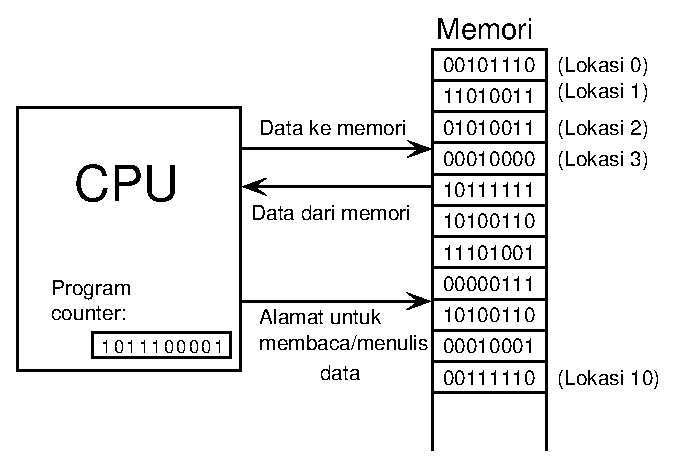
\includegraphics[scale=0.8]{images/overview_fig1.eps}
}





   



\section[Asynchronous Events]{Asynchronous Events: Polling Loops and Interrupts}\label{overview.2}

    

\start{{\Large C}PU menghabiskan sebagian besar waktunya} untuk mengambil
instruksi dari memori dan mengeksekusinya. Tetapi, CPU dan memori utama hanyalah
dua diantara banyak komponen pada sistem komputer nyata. Sistem
yang lengkap dari komputer mencakup beberapa perangkat seperti:



\mylist{

\myitem H\newword{ard disk} atau \newword{solid state drive} untuk menyimpan berkas program dan
data. (Perlu diingat bahwa memori utama hanya memegang sejumlah informasi
yang relatif kecil dan memegangnya selama sumber daya tetap nyala.
Hard disk atau solid state drive digunakan sebagai tempat penyimpanan permanen untuk jumlah informasi
yang lebih besar, tetapi program harus dimuat dari disk ke memori utama sebelum
program tersebut dieksekusi.  Hard disk menyimpan data pada piringan magnetis yang
berputar, sedangan solid state drive merupakan perangkat elektronis murni tanpa
bagian yang bergerak.)
\myitem \newword{Keyboard} dan \newword{mouse} untuk masukan pengguna.
\myitem \newword{Monitor} dan \newword{printer} yang digunakan untuk menampilkan
keluaran komputer.
\myitem \newword{Perangkat keluaran audio} yang memungkinan komputer untuk
mengeluarkan suara.
\myitem \newword{Antarmuka jaringan} yang memungkinkan komputer untuk
berkomunikasi dengan komputer lainnya yang terhubung dengannya pada sebuah jaringan,
baik secara nirkabel atau dengan kabel.
\myitem \newword{Scanner} yang mengubah gambar ke kode dalam bilangan
biner yang dapat disimpan dan diolah oleh komputer.
}



Daftar perangkat ini bisa ditambahkan lagi, ini karena sistem komputer dibangun
sedemikian rupa sehingga dapat dilakukan penambahan perangkat baru dengan mudah.
Terkadang CPU harus berkomunikasi dan mengontrol perangkat-perangkat tersebut. 
CPU hanya bisa melakukan hal ini dengan mengeksekusi instruksi bahasa mesin
(hanya inilah yang bisa dilakukan CPU, titik). Cara kerjanya adalah untuk setiap
perangkat di sistem terdapat sebuah \newword{driver perangkat}, yang
terdiri dari perangkat lunak yang akan dieksekusi CPU saat sedang
berurusan dengan perangkat tersebut. Pemasangan perangkat baru pada sistem
umumnya terdiri dari dari langkah: menghubungkan perangkat secara fisik ke
komputer, dan memasang perangkat lunak driver dari perangkat.
Tanpa driver dari perangkat, perangkat fisik saja akan tidak berguna, karena
CPU tidak akan bisa berkomunikasi dengan perangkat tersebut.


\mybreak



Sebuah sistem komputer yang terdiri dari banyak perangkat biasanya
diorganisasikan dengan menggabungkan satu perangkat dengan perangkat lainnya ke
satu atau lebih \newword{bus}. Sebuah bus merupakan sebuah kumpulan
kabel yang membawa berbagai macam informasi diantara perangkat-perangkat yang terhubung
ke kabel-kabel tersebut. Kabel-kabel ini membawa data, alamat, dan sinyal kontrol.
Sebuah alamat akan mengarahkan data ke perangkat tertentu dan kemungkinan ke sebuah
register tertentu atau lokasi tertentu dari perangkat tersebut. Sinyal kontrol dapat digunakan
, sebagai contoh, oleh sebuah perangkat untuk memberitahukan perangkat lain bahwa
data telah tersedia di bus data untuk perangkatnya. Sebuah sistem komputer sederhana dapat di
organisasikan sebagai berikut:


\par\dumpfigure{
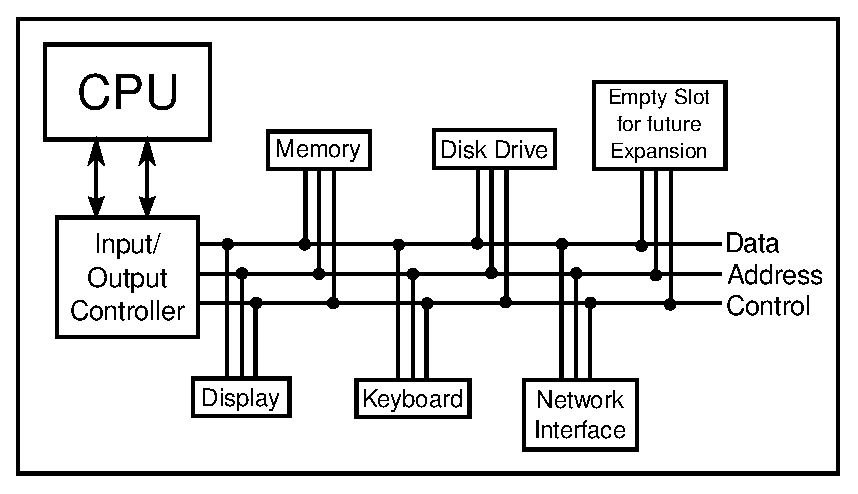
\includegraphics[scale=0.8]{images/overview-fig2.eps}
}




Saat ini, perangkat seperti keyboard, mouse, dan antarmuka jaringan dapat menghasilkan
masukan yang perlu untuk diproses oleh CPU. Bagaiaman CPU mengetahui bahwa data telah ada?
? Salah satu gagasan sederhana, yang tidak memuaskan, adalah
CPU tetap memeriksa data yang masuk secara berulang-ulang. Saat CPU menemukan data, 
ia memproses data tersebut. Metode ini disebut \newword{polling}, 
dikarenakan CPU menjajaki perangkat masukan secara berkala
untuk mencari tahu apakah perangkat memiliki masukan data untuk dilaporkan.
Sayangnya, meskipun polling sangat sederhana, metode ini juga sangat tidak efisien.
CPU dapat menghabiskan banyak waktu hanya untuk menunggu masukan.


Untuk menghindari ketidakefisienan ini, \newword{interupsi} lebih 
sering digunakan sebagai pengganti polling. Interupsi merupakan sinyal yang dikirimkan
oleh perangkat lain ke CPU. CPU merespon sinyal interrupt dengan mengesampingkan apapun
yang dilakukannya untuk merespon interupsi tersebut. Setelah CPU telah menangani
interupsi tersebut, CPU akan kembali ke hal yang dilakukannya sebelum interupsi terjadi.
Sebagai contoh, saat kamu menekan tombol di keyboard komputer maka sebuah interupsi keyboard
dikirimkan ke CPU. CPU akan merespon sinyal tersebut dengan menginterupsi yang sedang dilakukannya,
membaca tombol yang kamu tekan, memprosesnya, dan kembali ke pekerjaan yang dilakukan CPU
sebelum kamu menekan tombol tersebut.


Again, you should understand that this is a purely mechanical process: A
device signals an interrupt simply by turning on a wire. The CPU is built so
that when that wire is turned on, the CPU saves enough information about what it is
currently doing so that it can return to the same state later. This information
consists of the contents of important internal registers such as the program
counter. Then the CPU jumps to some predetermined memory location and begins
executing the instructions stored there. Those instructions make up an
\newword{interrupt handler} that does the processing
necessary to respond to the interrupt. (This interrupt handler is part of the
device driver software for the device that signaled the interrupt.) At the end
of the interrupt handler is an instruction that tells the CPU to jump back to
what it was doing; it does that by restoring its previously saved state.


Interrupts allow the CPU to deal with \newword{asynchronous events}. 
In the regular fetch-and-execute cycle, things happen in a
predetermined order; everything that happens is ``synchronized" with everything
else. Interrupts make it possible for the CPU to deal efficiently with events
that happen ``asynchronously," that is, at unpredictable times.


As another example of how interrupts are used, consider what happens when
the CPU needs to access data that is stored on a hard disk. The CPU can
access data directly only if it is in main memory. Data on the disk has to be copied
into memory before it can be accessed. Unfortunately, on the scale of speed at
which the CPU operates, the disk drive is extremely slow. When the CPU needs
data from the disk, it sends a signal to the disk drive telling it to locate
the data and get it ready. (This signal is sent synchronously, under the
control of a regular program.) Then, instead of just waiting the long and
unpredictable amount of time that the disk drive will take to do this, the CPU goes
on with some other task. When the disk drive has the data ready, it sends an
interrupt signal to the CPU. The interrupt handler can then read the requested
data.


\mybreak



Now, you might have noticed that all this only makes sense if the CPU
actually has several tasks to perform. If it has nothing better to do, it might
as well spend its time polling for input or waiting for disk drive operations
to complete. All modern computers use \newword{multitasking}
to perform several tasks at once. Some computers can be used by several people
at once. Since the CPU is so fast, it can quickly switch its attention from one
user to another, devoting a fraction of a second to each user in turn. This
application of multitasking is called \newword{timesharing}.
But a modern personal computer with just a single user also uses multitasking. For
example, the user might be typing a paper while a clock is continuously
displaying the time and a file is being downloaded over the network.


Each of the individual tasks that the CPU is working on is called a
\newword{thread}. (Or a \newword{process};
there are technical differences between threads and
processes, but they are not important here, since it is threads that
are used in Java.)  Many CPUs can literally execute more than one thread
simultaneously---such CPUs contain multiple ``cores," each of which can
run a thread---but there is always a limit on the number of threads
that can be executed at the same time.  Since there are often more threads
than can be executed simultaneously, the computer has to be able switch its
attention from one thread to another, just as a timesharing computer
switches its attention from one user to another.  In general, a 
thread that is being executed will continue to run
until one of several things happens:



\mylist{

\myitem The thread might voluntarily \newword{yield} control, to
give other threads a chance to run.
\myitem The thread might have to wait for some asynchronous event to occur. For
example, the thread might request some data from the disk drive, or it might
wait for the user to press a key. While it is waiting, the thread is said to be
\newword{blocked}, and other threads, if any, have a chance to run.
When the event occurs, an interrupt will ``wake up" the thread so that it can
continue running.
\myitem The thread might use up its allotted slice of time and be suspended to
allow other threads to run. Not all computers can ``forcibly" suspend a thread
in this way; those that can are said to use \newword{preemptive multitasking}. 
To do preemptive multitasking, a computer needs a special
timer device that generates an interrupt at regular intervals, such as 100
times per second. When a timer interrupt occurs, the CPU has a chance to switch
from one thread to another, whether the thread that is currently running likes
it or not.  All modern desktop and laptop computers, and even typical smartphones and tablets, 
use preemptive multitasking.
}



Ordinary users, and indeed ordinary programmers, have no need to deal with
interrupts and interrupt handlers. They can concentrate on the different tasks
or threads that they want the computer to perform; the details of how the
computer manages to get all those tasks done are not important to them. In
fact, most users, and many programmers, can ignore threads and multitasking
altogether. However, threads have become increasingly important as computers
have become more powerful and as they have begun to make more use of
multitasking and multiprocessing.  In fact, the ability to work with threads
is fast becoming an essential job skill for programmers.
Fortunately, Java has good support for threads, which
 are built into the Java programming language as a
fundamental programming concept.  Programming with threads will be covered
in Chapter~\ref{threads}.


Just as important in Java and in modern programming in general is the basic
concept of asynchronous events. While programmers don't actually deal with
interrupts directly, they do often find themselves writing \newword{event handlers}, 
which, like interrupt handlers, are called
asynchronously when specific events occur. Such ``event-driven programming" has
a very different feel from the more traditional straight-through, synchronous
programming. We will begin with the more traditional type of programming, which
is still used for programming individual tasks, but we will return to threads
and events later in the text, starting in Chapter~\ref{GUI1}


\mybreak



By the way, the software that does all the interrupt handling, handles
communication with the user and with hardware devices, and controls which thread
is allowed to run is called the
\newword{operating system}. The operating system is the
basic, essential software without which a computer would not be able to
function. Other programs, such as word processors and Web browsers,
are dependent upon the operating system. Common operating systems include
Linux, various versions of Windows, and Mac~OS.
    
    

   



\section{Mesin Virtual Java}\label{overview.3}

    

\start{{\Large B}ahasa mesin mencakup} instruksi yang sangat sederhana
yang dapat dieksekusi langsung oleh komputer CPU. Hampir semua program
ditulis dalam \newword{bahasa pemrograman tingkat tinggi} 
seperti Java, Pascal, atau C++. Program yang ditulis dalam bahasa pemrograman
tingkat tinggi tidaklah dapat dijalankan langsung di komputer. Karena itu, program
harus diterjemahkan ke bahasa mesin. Penerjemahan ini dapat dilakukan oleh sebuah
program yang disebut \newword{kompiler}. Kompiler menerima
program dengan bahasa pemrograman tingkat tinggi dan menterjemahkannya menjadi
program dalam bahasa mesin yang dapat dieksekusi. Setelah proses terjemahan selesai,
program dalam bahasa mesin tersebut dapat dijalankan berkali-kali, tetapi
program tersebut hanya bisa dijalankan di komputer yang sesuai dengan jenis bahasa mesin 
yang sama (hal ini dikarenakan setiap jenis komputer memiliki bahasa mesinnya
tersendiri). Jika program akan dijalankan ke jenis komputer yang lain, maka program tersebut
harus diterjemahkan ulang menggunakan kompilator yang berbeda, menjadi bahasa mesin
yang sesuai dengan komputer tersebut.


Ada alternatif lain dari mengkompilasi program dalam bahasa tingkat tinggi. Alih-alih
menggunakan kompilator, yang menerjemahan program sekaligus dalam satu waktu, kita dapat menggunakan
\newword{interpreter}, yang menterjemahkan instruksi demi instruksi di saat
dibutuhkan. Interpreter merupakan program yang bekerja mirip seperti CPU,
dengan semacam siklus ambil-dan-eksekusinya. Dalam mengeksekusi program
, interpreter berjalan dalam satu simpul yang didalamnya ia melakukan pembacaan satu
instruksi dari program dalam satu waktu secara terus menerus, menentukan apa yang
diperlukan untuk melakukan instruksi tersebut, dan kemudian melakukan perintah
bahasa mesin yang sesuai dengan instruksi tersebut.
so.


Salah satu kegunaan dari interpreter adalah untuk mengeksekusi program dalam 
bahasa tingkat tinggi. Sebagai contoh, bahasa pemrograman Lisp biasanya dieksekusi
oleh interpreter daripada kompilator. Selain itu, interpreter
memiliki tujuan lain: interpreter dapat memampukan kita untuk menggunakan sebuah
program dalam bahasa mesin yang ditujukan untuk komputer jenis tertentu ke
jenis komputer yang berbeda. Sebagai contoh, ada sebuah program yang disebut 
``Virtual PC" yang berjalan di komputer Mac~OS. Virtual PC merupakan interpreter
yang mengeksekusi program dalam bahasa mesin yang ditulis untuk komputer klon IBM-PC. 
Jika kita menjalankan Virtual PC di Mac~OS, kita dapat menjalankan program PC apa pun,
termasuk program yang ditulis untuk Windows.(Sayangnya, program PC akan berjalan jauh
lebih lambat dari klon IBM yang sebenarnya. Masalahnya dikarenakan Virtual PC
mengeksekusi beberapa instruksi bahasa mesin Mac~OS untuk setiap instruksi
bahasa mesin PC di dalam program yang ditafsirkannya. Program yang dikompilasi secara
inheren lebih cepat dari program yang ditafsirkan .)


\mybreak



Para perancang Java memilih untuk menggunakan gabungan dari kompilasi dan interpretasi.
Program yang ditulis di Java dikompilasi ke bahasa mesin, tetapi ke dalam bahasa mesin
dari komputer yang tidak ada. Komputer ``Virtual" ini dikenal sebagai 
\newword{Java Virtual Machine} atau JVM.
Bahasa mesin dari Java Virtual Machine disebut \newword{bytecode Java}.
Tidak ada alasan yang membatasi bytecode Java hanya digunakan di komputer virtual daripada digunakan
sebagai bahasa mesin di komputer nyata. Namun penggunaan mesin virtual merupakan
salah satu nilai jual dari Java: dapat digunakan di \textbf{berbagai jenis} komputer. Yang
dibutuhkan oleh komputer-komputer tersebut adalah sebuah interpreter untuk bytecode Java.
Intepreter ini mensimulasikan JVM seperti PC Virtual mensimulasikan sebuah komputer nyata.
(Istilah JVM juga berarti program intrepreter untuk bytecode Java yang melakukan simulasi,
jadi kita mengartikan komputer memerlukan sebuah JVM untuk menjalankan program Java.
Secara teknis, lebih tepat untuk mengatakan bahwa interpreter \textit{mengimplementasikan}
JVM daripada mengatakannya merupakan sebuah JVM.)


Tentu saja dibutuhkan interpreter bytecode Java yang berbeda untuk tiap jenis
komputer, tetapi setelah sebuah komputer memiliki interpreter bytecode Java, ia
dapat menjalankan berbagai program bytecode Java. Dan program bytecode Java yang sama
dapat dijalankan di berbagai komputer yang memiliki interpreter tersebut. Hal inilah
yang menjadi fitur utama dari Java: satu program yang telah dikompilasi dapat
dijalankan di berbagai tipe komputer tanpa perlu melakukan perubahan.


\par\dumpfigure{
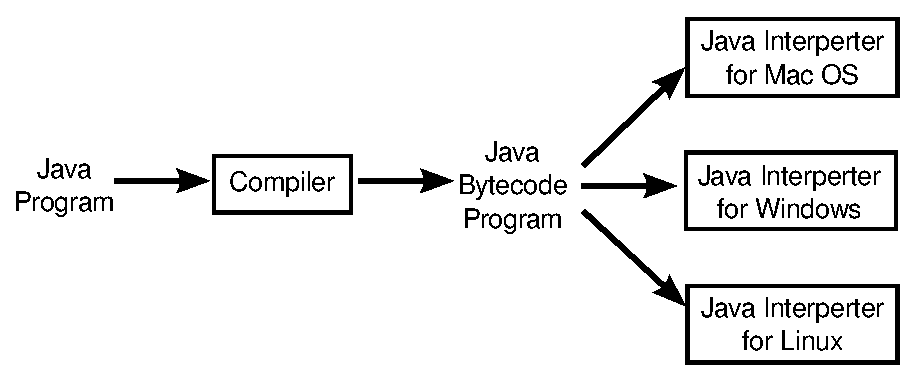
\includegraphics[scale=0.8]{images/overview-fig3.eps}
}



Mungkin kamu bertanya mengapa menggunakan bytecode Java sebagai perantara?
mengapa tidak membagikan saja program Java orisinilnya dan mempersilahkan tiap
orang mengkompilasinya ke bahasa mesin dari komputer jenis apapun yang mereka
miliki dan menjalankannya di situ?. Ada banyak alasannya. Yang pertama, kompiler
harus mengerti Java, yang merupakan bahasa tingkat tinggi. Kompiler itu sendiri
pun merupakan program yang kompleks. intrepreter bytecode Java, di sisi lain,
merupakan program yang cukup sederhana. Sehingga mudah untuk membuat interpreter
bytecode untuk jenis komputer baru; setelah interpreter berhasil dibangun, komputer
tersebut dapat menjalankan program Java terkompilasi apapun. Jauh lebih sulit
untuk membuat kompiler Java untuk komputer yang sama.


Lebih lanjut lagi, banyak program Java yang dibuat agar dapat didownload melalui
jaringan. Hal ini memunculkan masalah keamanan yang nyata: kamu tentu tidak mau
mendownload dan menjalankan program yang akan merusak komputer atau berkasmu.
Interpreter bytecode berperan sebagai sebuah pelindung antara kamu dan program yang
kamu download. Kamu benar-benar menjalankan interpreter yang menjalankan program
yang kamu download secara tidak langsung. Intepreter dan melindungimu dari bahaya
potensial yang mungkin ada di dalam program tersebut.


 Saat dimana Java merupakan bahasa pemrograman baru, Java dikritik sebagai
bahasa pemrograman yang lambat kinerjanya: Karena bytecode Java dijalankan
oleh interpreter, di mana program bytecode Java tidak akan pernah berjalan
secepat program yang dikompilasi ke dalam bahasa mesin aslinya (yakni bahasa
mesin aktual dari komputer di mana program dijalankan)
Tetapi masalah ini telah diatasi secara hampir menyeluruh dengan penggunaan
\newword{kompiler just-in-time} untuk menjalankan bytecode Java.
Kompiler just-in-time akan menerjemahkan bytecode Java ke dalam bahasa mesin asli.
Ia melakukannya di saat menjalankan program.  Sama halnya dengan interpreter
normal, masukan dari kompiler just-in-time merupakan program bytecode Java,
dan tugasnya adalah menjalankan program tersebut. Tetapi saat menjalankan program,
ia juga menerjemahkan bagian-bagian dari program ke bahasa mesin. Bagian yang
diterjemahkan dari program dapat dijalankan lebih cepat daripada dengan interpretasi.
Karena sebagian dari program sering dieksekusi saat program bekerja, maka
kompiler just-in-time dapat meningkatkan kecepatan dari keseluruhan waktu eksekusi
secara signifikan.



Perlu saya garisbawahi bahwa tidak ada hubungan yang khusus antara Java
dan bytecode Java. Program yang ditulis dengan bahasa Java tentu saja dapat
dikompilasi ke bahasa mesin dari komputer nyata. Dan program yang ditulis dengan
bahasa lain dapat dikompilasi menjadi bytecode Java. Tetapi kombinasi dari Java
dan bytecode Java lah yang independen terhadap platform, aman, dan kompatibel
terhadap jaringan sekaligus memampukan kamu untuk memprogram dengan bahasa
pemrograman tingkat tinggi berbasis objek.



(Dalam beberapa tahun belakangan ini, telah menjadi hal yang lumrah untuk
menciptakan bahasa pemrograman baru, atau versi dari bahasa lama, yang dapat
dikompilasi menjadi bytecode Java.  Program bytecode Java yang telah dikompilasi
tersebut kemudian dapat dieksekusi oleh JVM standar. Bahasa-bahasa baru yang
telah dibangun secara khusus untuk JVM termasuk Groovy, Clojure, dan Processing.
  Jython dan JRuby merupakan versi dari bahasa yang lebih lama yang ditujukan
untuk JVM. Bahasa-bahasa ini memberikan kemungkinan untuk memanfaatkan keuntungan
dari penggunaan JVM namun menghindari segi-segi teknis dari bahasa Java.
  Kenyataannya, penggunaan bahasa lain dengan JVM menjadi cukup penting sehingga
beberapa fitur telah ditambahkan ke JVM di Java Versi~7 yang ditujukan
untuk memberikan dukungan lebih baik bagi beberapa dari bahasa tersebut.)


\mybreak



Saya juga perlu memberikan sedikit catatan bahwa bagian terberat dari independen
terhadap platform adalah menyediakan ``Grafis Antarmuka Pengguna"---dengan window, 
tombol-tombol, dan sebagainya.---yang akan bekerja pada semua platform yang
mendukung Java. Kamu akan melihat masalah ini lebih lanjut di Section~\ref{overview.6}.


   



\section[Building Blocks of Programs]{Fundamental Building Blocks of Programs}\label{overview.4}

    

\start{{\Large T}here are two basic aspects} of programming: data
and instructions. To work with data, you need to understand \newword{variables} 
and \newword{types}; to work with
instructions, you need to understand \newword{control structures} 
and \newword{subroutines}. You'll spend a
large part of the course becoming familiar with these concepts.


A \newword{variable} is just a memory location (or
several consecutive locations treated as a unit) that has been given a name so that it can
be easily referred to and used in a program. The programmer only has to worry
about the name; it is the compiler's responsibility to keep track of the memory
location. As a programmer, you need to keep in mind that the name refers to a
kind of ``box" in memory that can hold data, even though you don't have
to know where in memory that box is located.


In Java and in many other programming languages, a variable has a \newword{type}
that indicates what sort of data it can hold. One type of
variable might hold integers---whole numbers such as 3, -7, and 0---while
another holds floating point numbers---numbers with decimal points such as
3.14, -2.7, or 17.0. (Yes, the computer does make a distinction between the
integer 17 and the floating-point number 17.0; they actually look quite
different inside the computer.) There could also be types for individual
characters ('A', ';', etc.), strings (``Hello", ``A string can include many
characters", etc.), and less common types such as dates, colors, sounds, or any
other kind of data that a program might need to store.


Programming languages always have commands for getting data into and out of
variables and for doing computations with data. For example, the following
``assignment statement," which might appear in a Java program, tells the
computer to take the number stored in the variable named ``principal", multiply
that number by 0.07, and then store the result in the variable named
``interest":

\displaycode{interest = principal * 0.07;}\donedisplaycode


\noindent There are also ``input commands" for getting data from the user or from files
on the computer's disks, and there are ``output commands" for sending data in the other
direction.


These basic commands---for moving data from place to place and for
performing computations---are the building blocks for all programs. These
building blocks are combined into complex programs using control structures and
subroutines.


\mybreak



A program is a sequence of instructions. In the ordinary ``flow of control,"
the computer executes the instructions in the sequence in which they occur in the program,
one after the other. However, this is obviously very limited: the computer
would soon run out of instructions to execute. \newword{Control structures} 
are special instructions that can change the flow of control.
There are two basic types of control structure: \newword{loops},
which allow a sequence of instructions to be repeated
over and over, and \newword{branches}, which allow the
computer to decide between two or more different courses of action by testing
conditions that occur as the program is running.


For example, it might be that if the value of the variable ``principal" is
greater than 10000, then the ``interest" should be computed by multiplying the
principal by 0.05; if not, then the interest should be computed by multiplying
the principal by 0.04. A program needs some way of expressing this type of
decision. In Java, it could be expressed using the following ``if
statement":

\displaycode{if (principal \> 10000)
    interest = principal * 0.05;
else
    interest = principal * 0.04;}\donedisplaycode


\noindent (Don't worry about the details for now. Just remember that the computer can
test a condition and decide what to do next on the basis of that test.)


Loops are used when the same task has to be performed more than once. For
example, if you want to print out a mailing label for each name on a mailing
list, you might say, ``Get the first name and address and print the label; get
the second name and address and print the label; get the third name and address
and print the label\dots" But this quickly becomes ridiculous---and might not
work at all if you don't know in advance how many names there are. What you
would like to say is something like ``While there are more names to process, get
the next name and address, and print the label." A loop can be used in a
program to express such repetition.


\mybreak



Large programs are so complex that it would be almost impossible to write
them if there were not some way to break them up into manageable ``chunks."
Subroutines provide one way to do this. A \newword{subroutine} 
consists of the instructions for performing some
task, grouped together as a unit and given a name. That name can then be used
as a substitute for the whole set of instructions. For example, suppose that
one of the tasks that your program needs to perform is to draw a house on the
screen. You can take the necessary instructions, make them into a subroutine,
and give that subroutine some appropriate name---say, ``drawHouse()". Then
anyplace in your program where you need to draw a house, you can do so with the
single command:

\displaycode{drawHouse();}\donedisplaycode


\noindent This will have the same effect as repeating all the house-drawing
instructions in each place.


The advantage here is not just that you save typing. Organizing your program
into subroutines also helps you organize your thinking and your program design
effort. While writing the house-drawing subroutine, you can concentrate on the
problem of drawing a house without worrying for the moment about the rest of
the program. And once the subroutine is written, you can forget about the
details of drawing houses---that problem is solved, since you have a
subroutine to do it for you. A subroutine becomes just like a built-in part of
the language which you can use without thinking about the details of what goes
on ``inside" the subroutine.


\mybreak



Variables, types, loops, branches, and subroutines are the basis of what
might be called ``traditional programming." However, as programs become larger,
additional structure is needed to help deal with their complexity. One of the
most effective tools that has been found is object-oriented programming, which
is discussed in the next section.


   



\section[Object-oriented Programming]{Objects and Object-oriented Programming}\label{overview.5}



\start{{\Large P}rograms must be designed}. No one can just sit down
at the computer and compose a program of any complexity. The discipline called
\newword{software engineering} is concerned with the
construction of correct, working, well-written programs. The software engineer
tries to use accepted and proven methods for analyzing the problem to be solved
and for designing a program to solve that problem.


During the 1970s and into the 80s, the primary software engineering
methodology was \newword{structured programming}. The
structured programming approach to program design was based on the following
advice: To solve a large problem, break the problem into several pieces and
work on each piece separately; to solve each piece, treat it as a new problem
which can itself be broken down into smaller problems; eventually, you will
work your way down to problems that can be solved directly, without further
decomposition. This approach is called \newword{top-down programming}.


There is nothing wrong with top-down programming. It is a valuable and
often-used approach to problem-solving. However, it is incomplete. For one
thing, it deals almost entirely with producing the
\textbf{instructions} necessary to solve a problem. But as time went
on, people realized that the design of the \textbf{data structures} for
a program was at least as important as the design of subroutines and control
structures. Top-down programming doesn't give adequate consideration to the
data that the program manipulates.


Another problem with strict top-down programming is that it makes it
difficult to reuse work done for other projects. By starting with a particular
problem and subdividing it into convenient pieces, top-down programming tends
to produce a design that is unique to that problem. It is unlikely that you
will be able to take a large chunk of programming from another program and fit
it into your project, at least not without extensive modification. Producing
high-quality programs is difficult and expensive, so programmers and the people
who employ them are always eager to reuse past work.


\mybreak



So, in practice, top-down design is often combined with \newword{bottom-up design}. 
In bottom-up design, the approach is to
start ``at the bottom," with problems that you already know how to solve (and
for which you might already have a reusable software component at hand). From
there, you can work upwards towards a solution to the overall problem.


The reusable components should be as ``modular" as possible. A \newword{module}
is a component of a larger system that interacts with
the rest of the system in a simple, well-defined, straightforward manner. The
idea is that a module can be ``plugged into" a system. The details of what goes
on inside the module are not important to the system as a whole, as long as the
module fulfills its assigned role correctly. This is called \newword{information hiding}, 
and it is one of the most important
principles of software engineering.


One common format for software modules is to contain some data, along with
some subroutines for manipulating that data. For example, a mailing-list module
might contain a list of names and addresses along with a subroutine for adding
a new name, a subroutine for printing mailing labels, and so forth. In such
modules, the data itself is often hidden inside the module; a program that uses
the module can then manipulate the data only indirectly, by calling the
subroutines provided by the module. This protects the data, since it can only
be manipulated in known, well-defined ways. And it makes it easier for programs
to use the module, since they don't have to worry about the details of how the
data is represented. Information about the representation of the data is
hidden.


Modules that could support this kind of information-hiding became common in
programming languages in the early 1980s. Since then, a more advanced form of
the same idea has more or less taken over software engineering. This latest
approach is called \newword{object-oriented programming},
often abbreviated as OOP.


The central concept of object-oriented programming is the \newword{object}, 
which is a kind of module containing data and
subroutines. The point-of-view in OOP is that an object is a kind of
self-sufficient entity that has an internal \newword{state}
(the data it contains) and that can respond to \newword{messages} 
(calls to its subroutines). A mailing list object,
for example, has a state consisting of a list of names and addresses. If you
send it a message telling it to add a name, it will respond by modifying its
state to reflect the change. If you send it a message telling it to print
itself, it will respond by printing out its list of names and addresses.


The OOP approach to software engineering is to start by identifying the
objects involved in a problem and the messages that those objects should
respond to. The program that results is a collection of objects, each with its
own data and its own set of responsibilities. The objects interact by sending
messages to each other. There is not much ``top-down" in the large-scale design of such a program, and
people used to more traditional programs can have a hard time getting used to
OOP. However, people who use OOP would claim that object-oriented programs tend
to be better models of the way the world itself works, and that they are
therefore easier to write, easier to understand, and more likely to be
correct.


\mybreak



You should think of objects as ``knowing" how to respond to certain messages.
Different objects might respond to the same message in different ways. For
example, a ``print" message would produce very different results, depending on
the object it is sent to. This property of objects---that different objects
can respond to the same message in different ways---is called \newword{polymorphism}.


It is common for objects to bear a kind of ``family resemblance" to one
another. Objects that contain the same type of data and that respond to the
same messages in the same way belong to the same \newword{class}. 
(In actual programming, the class is primary; that is,
a class is created and then one or more objects are created using that class as
a template.) But objects can be similar without being in exactly the same
class.


For example, consider a drawing program that lets the user draw lines,
rectangles, ovals, polygons, and curves on the screen. In the program, each
visible object on the screen could be represented by a software object in the
program. There would be five classes of objects in the program, one for each
type of visible object that can be drawn. All the lines would belong to one
class, all the rectangles to another class, and so on. These classes are
obviously related; all of them represent ``drawable objects." They would, for
example, all presumably be able to respond to a ``draw yourself" message.
Another level of grouping, based on the data needed to represent each type of
object, is less obvious, but would be very useful in a program: We can group
polygons and curves together as ``multipoint objects," while lines, rectangles,
and ovals are ``two-point objects." (A line is determined by its two endpoints, a
rectangle by two of its corners, and an oval by two corners of the rectangle
that contains it.  The rectangles that I am talking about here have
sides that are vertical and horizontal, so that they can be specified by just
two points; this is the common meaning of ``rectangle" in drawing programs.) 
We could diagram these relationships as follows:


\par\dumpfigure{
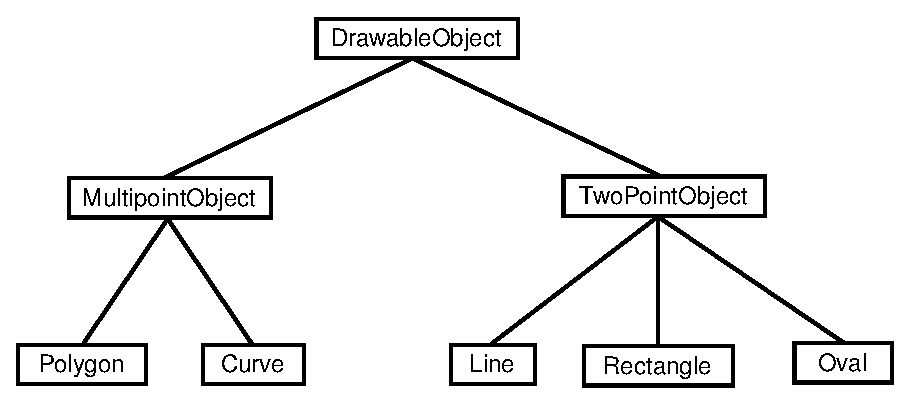
\includegraphics[scale=0.8]{images/overview-fig4.eps}
}



DrawableObject, MultipointObject, and TwoPointObject would be classes in the
program. MultipointObject and TwoPointObject would be \newword{subclasses}
of DrawableObject. The class Line would be a
subclass of TwoPointObject and (indirectly) of DrawableObject. A subclass of a
class is said to \newword{inherit} the properties of that
class. The subclass can add to its inheritance and it can even ``override" part
of that inheritance (by defining a different response to some method).
Nevertheless, lines, rectangles, and so on \textbf{are} drawable
objects, and the class DrawableObject expresses this relationship.


Inheritance is a powerful means for organizing a program. It is also related
to the problem of reusing software components. A class is the ultimate reusable
component. Not only can it be reused directly if it fits exactly into a program
you are trying to write, but if it just almost fits, you can still reuse it by
defining a subclass and making only the small changes necessary to adapt it
exactly to your needs.


So, OOP is meant to be both a superior program-development tool and a
partial solution to the software reuse problem. Objects, classes, and
object-oriented programming will be important themes throughout the rest of
this text.  You will start using objects that are built into the Java
language in the next chapter, and in
Chapter~\ref{OOP} you will begin creating your own classes and objects.


   



\section{The Modern User Interface}\label{overview.6}



\start{{\Large W}hen computers were first introduced}, ordinary
people---including most programmers---couldn't get near them. They were
locked up in rooms with white-coated attendants who would take your programs
and data, feed them to the computer, and return the computer's response some
time later. When timesharing---where the computer switches its attention
rapidly from one person to another---was invented in the 1960s, it became
possible for several people to interact directly with the computer at the same
time. On a timesharing system, users sit at ``terminals" where they type
commands to the computer, and the computer types back its response. Early
personal computers also used typed commands and responses, except that there
was only one person involved at a time. This type of interaction between a user
and a computer is called a \newword{command-line interface}.


Today, of course, most people interact with computers in a completely
different way. They use a \newword{Graphical User Interface}, 
or GUI. The computer draws interface \newword{components} on the
screen. The components include things like windows, scroll bars, menus,
buttons, and icons. Usually, a \newword{mouse} is used to
manipulate such components or, on ``touchscreens," your fingers.
Assuming that you have not just been teleported in
from the 1970s, you are no doubt already familiar with the basics of graphical user
interfaces!


A lot of GUI interface components have become fairly standard. That is, they
have similar appearance and behavior on many different computer platforms
including Mac~OS, Windows, and Linux. Java programs,
which are supposed to run on many different platforms without modification to
the program, can use all the standard GUI components. They might vary a little in
appearance from platform to platform, but their functionality should be
identical on any computer on which the program runs.


Shown below is an image of a very simple Java program that demonstrates
a few standard GUI interface components.  When the program is run, a window
similar to the picture shown here will open on the computer screen.
There are four components in the window with which the user can interact: 
a button, a checkbox, a text field, and
a pop-up menu. These components are labeled. There are a few other components
in the window. The labels themselves are components (even though you can't
interact with them). The right half of the window is a text area component,
which can display multiple lines of text. A~scrollbar component appears
alongside the text area when the number of lines of text becomes larger
than will fit in the text area.  And in fact, in Java terminology, the
whole window is itself considered to be a ``component."


\par\dumpfigure{
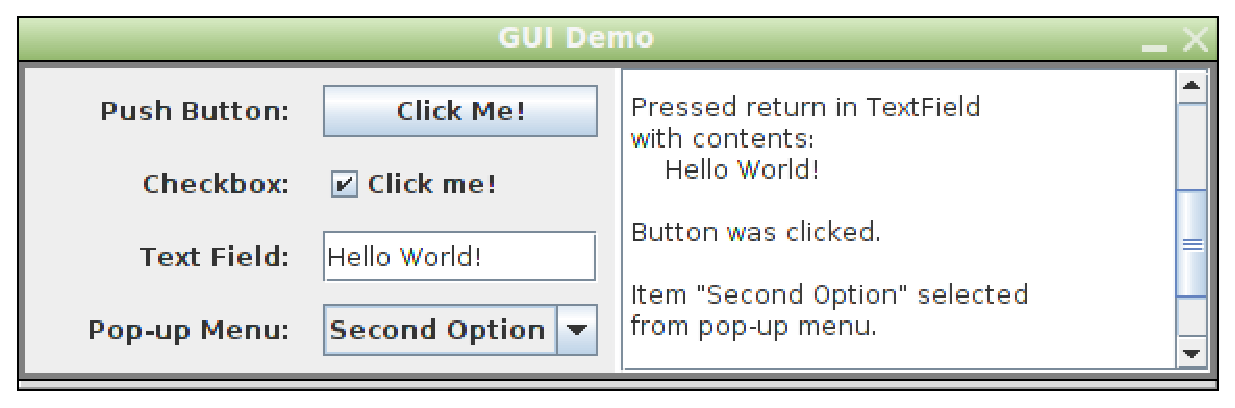
\includegraphics[scale=0.5]{images/overview-GUIDemo.eps}
}

    
\noindent (If you would like to run this program, the source code, \sourceref{GUIDemo.java},
as well as a compiled program, \jarref{GUIDemo.jar}, are available on line.  For more information on using
this and other examples from this textbook, see Section~\ref{basics.6}.)


Now, Java actually has two complete sets of GUI components. One of these,
the AWT or \newword{Abstract Windowing Toolkit}, was
available in the original version of Java. The other, which is known as
\newword{Swing}, was introduced in Java version 1.2,
and is used in preference to the AWT in most modern Java programs.  The
program that is shown above uses components that are part of Swing. 



When a user interacts with GUI components,
``events" are generated.  For example, clicking a push button generates an event, and pressing
return while typing in a text field generates an event.
Each time an
event is generated, a message is sent to the program telling it that the event
has occurred, and the program responds according to its program. In fact, a typical GUI
program consists largely of ``event handlers" that tell the program how to respond
to various types of events. In this example, the program has been programmed
to respond to each event by displaying a message in the text area.
In a more realistic example, the event handlers would have more to do.


The use of the term ``message" here is deliberate. Messages, as you saw in
the previous~section, are sent to objects. In fact, Java
GUI components are implemented as objects. Java includes many predefined
classes that represent various types of GUI components. Some of these classes
are subclasses of others. Here is a diagram showing just a few of Swing's GUI classes
and their relationships:


\par\dumpfigure{
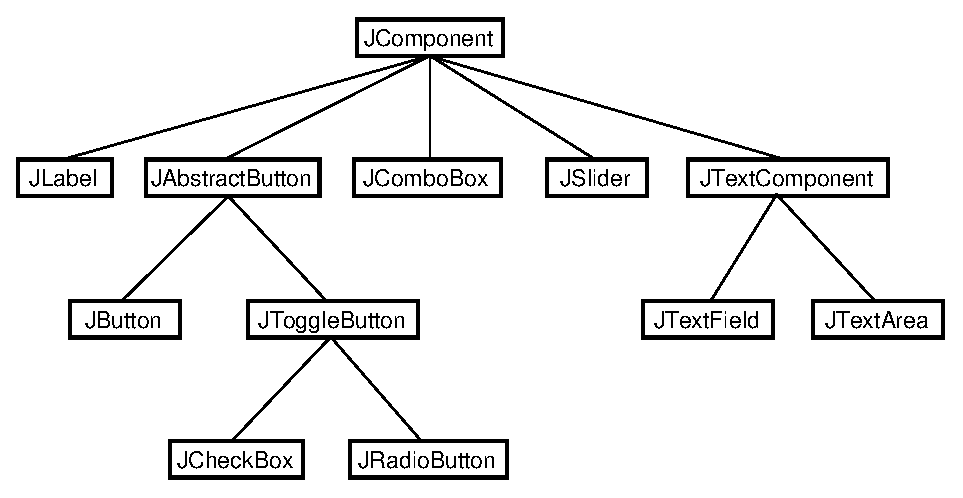
\includegraphics[scale=0.7]{images/overview-fig5.eps}
}



Don't worry about the details for now, but try to get some feel about how
object-oriented programming and inheritance are used here. Note that all the
GUI classes are subclasses, directly or indirectly, of a class called
\classname{JComponent}, which represents general properties
that are shared by all Swing components. In the diagram,
two of the direct subclasses of \classname{JComponent}
themselves have subclasses. The classes \classname{JTextArea} and
\classname{JTextField}, which have certain behaviors in common, are grouped
together as subclasses of \classname{JTextComponent}.
Similarly \classname{JButton} and \classname{JToggleButton}
are subclasses of \classname{JAbstractButton}, which represents
properties common to both buttons and checkboxes.  (\classname{JComboBox},
by the way, is the Swing class that represents pop-up menus.)



Just from this brief discussion, perhaps you can see how GUI programming can
make effective use of object-oriented design. In fact, GUIs, with their
``visible objects," are probably a major factor contributing to the popularity
of OOP.


Programming with GUI components and events is one of the most interesting
aspects of Java. However, we will spend several chapters on the basics before
returning to this topic in Chapter~\ref{GUI1}.
    

   



\section{The Internet and Beyond}\label{overview.7}



\start{{\Large C}omputers can be connected} together on \newword{networks}. 
A computer on a network can communicate with other
computers on the same network by exchanging data and files or by sending and
receiving messages. Computers on a network can even work together on a large
computation.


Today, millions of computers throughout the world are connected to a single
huge network called the \newword{Internet}. New computers
are being connected to the Internet every day, both by wireless communication
and by physical connection using technologies such as DSL, cable modems,
and Ethernet.


There are elaborate \newword{protocols} for communication
over the Internet. A protocol is simply a detailed specification of how
communication is to proceed. For two computers to communicate at all, they must
both be using the same protocols. The most basic protocols on the Internet are
the \newword{Internet Protocol} (IP), which specifies how
data is to be physically transmitted from one computer to another, and the
\newword{Transmission Control Protocol} (TCP), which ensures
that data sent using IP is received in its entirety and without error. These
two protocols, which are referred to collectively as TCP/IP, provide a
foundation for communication. Other protocols use TCP/IP to send specific types
of information such as web pages, electronic mail, and data files.


All communication over the Internet is in the form of \newword{packets}.
A packet consists of some data being sent from one
computer to another, along with addressing information that indicates where on
the Internet that data is supposed to go. Think of a packet as an envelope with
an address on the outside and a message on the inside. (The message is the
data.) The packet also includes a ``return address," that is, the address of the
sender. A packet can hold only a limited amount of data; longer messages must
be divided among several packets, which are then sent individually over the net
and reassembled at their destination.


Every computer on the Internet has an \newword{IP address}, 
a number that identifies it uniquely among all the computers on
the net. (Actually, the claim about uniqueness is not quite true, but
the basic idea is valid, and the full truth is complicated.)
The IP address is used for addressing packets. A computer can only
send data to another computer on the Internet if it knows that computer's IP
address. Since people prefer to use names rather than numbers, most computers
are also identified by names, called \newword{domain names}.
For example, the main computer of the Mathematics Department at Hobart and William Smith Colleges has the
domain name math.hws.edu. (Domain names are just for convenience; your computer
still needs to know IP addresses before it can communicate. There are computers
on the Internet whose job it is to translate domain names to IP addresses. When
you use a domain name, your computer sends a message to a domain name server to
find out the corresponding IP address. Then, your computer uses the IP address,
rather than the domain name, to communicate with the other computer.)


The Internet provides a number of services to the computers connected to it
(and, of course, to the users of those computers). These services use TCP/IP to
send various types of data over the net. Among the most popular services are
instant messaging, file sharing, electronic mail, and the World-Wide Web.
Each service has its own protocols, which are used to control transmission of
data over the network.  Each service also has some sort of user interface,
which allows the user to view, send, and receive data through the service.


For example, the email service uses a protocol known as \newword{SMTP}
(Simple Mail Transfer Protocol) to transfer email messages from one computer to another.
Other protocols, such as POP and IMAP, are used to fetch messages from an email
account so that the recipient can read them.  A person who uses email, however, 
doesn't need to understand or even know about these protocols.  Instead, they
are used behind the scenes by computer programs to send
and receive email messages.  These programs provide the user with an easy-to-use user interface
to the underlying network protocols.


The World-Wide Web is perhaps the most exciting of network services.  The World-Wide Web
allows you to request \newword{pages} of information that are stored on computers all over
the Internet.  A Web page can contain \newword{links} to other pages on the
same computer from which it was obtained or to other computers anywhere in the world.
A computer that stores such pages of information is called a
\newword{web server}.  The user interface to the Web is the type of
program known as a \newword{web browser}.  Common web browsers include 
Internet Explorer, Firefox, Chrome, and Safari.  You use a Web browser to
request a page of information.  The browser sends a request for that page to
the computer on which the page is stored, and when a response is received from that
computer, the web browser displays it to you in a neatly formatted form.
A web browser is just a user interface to the Web.  Behind the scenes, the
web browser uses a protocol called \newword{HTTP} (HyperText Transfer Protocol) 
to send each page request and to receive the response from the web server.



\mybreak



Now just what, you might be thinking, does all this have to do with Java? In
fact, Java is intimately associated with the Internet and the World-Wide Web.
When Java was first introduced, one of its big attractions was the ability
to write \newword{applets}.  An applet is a small program that is
transmitted over the Internet and that runs on a web page.  Applets make it
possible for a web page to perform complex tasks and have complex interactions
with the user.  Alas, applets have suffered from a variety of security problems,
and fixing those problems has made them more difficult to use.  Applets have
become much less common on the Web, and in any case, there are other options for
running programs on Web pages.



But applets are only one aspect of Java's relationship with the Internet.
Java can be used to write complex, stand-alone applications that do not depend
on a Web browser.  Many of these programs are network-related.  For example
many of the largest and most complex web sites use web server software
that is written in Java.  Java includes excellent support for network protocols,
and its platform independence makes it possible to write network programs
that work on many different types of computer.  You will learn about Java's
network support in Chapter~\ref{IO}.
   


Its support for networking is not Java's only advantage. But many good
programming languages have been invented only to be soon forgotten. Java has
had the good luck to ride on the coattails of the Internet's immense and increasing
popularity.


\mybreak



As Java has matured, its applications have reached far beyond the Net.
The standard version of Java already comes with support for many technologies, 
such as cryptography and data compression.  Free extensions are available to support
many other technologies such as advanced sound processing and three-dimensional
graphics.  Complex, high-performance systems can be developed in Java.  For example,
Hadoop, a system for large scale data processing, is written in Java. Hadoop is
used by Yahoo, Facebook, and other Web sites to process the huge amounts of data
generated by their users.


Furthermore, Java is not restricted to use on traditional computers.  Java can
be used to write programs for many smartphones (though not for the iPhone).
It is the primary development language for Android-based 
devices.  (Some mobile devices use
a version of Java called Java ME (``Mobile Edition"), but Android uses
Google's own version of Java and does not use the same graphical user interface
components as standard Java.)  Java is also the programming language
for the Amazon Kindle eBook reader and for interactive features on Blu-Ray
video disks.


At this time, Java certainly ranks as one of the most widely used programming
languages. It is a good choice for almost any programming project that
is meant to run on more than one type of computing device, and is
a reasonable choice even for many programs that will run on only one device.
It is probably still the most widely taught language at Colleges and Universities.
It is similar enough to other popular languages, such as C, C++, and Python, that
knowing it will give you a good start on learning those languages as well.
Overall, learning Java is a great starting point on the road to becoming an
expert programmer.  I hope you enjoy the journey!




   



\begin{quiz}

\quizquestion 
One of the components of a
computer is its \textit{CPU.} What is a CPU and what role does it play in a
computer?
\quizquestion 
Explain what is meant by an
``asynchronous event." Give some examples.
\quizquestion 
What is the difference
between a ``compiler" and an ``interpreter"?
\quizquestion 
Explain the difference
between \textit{high-level languages} and \textit{machine language.}
\quizquestion 
If you have the source code
for a Java program, and you want to run that program, you will need both a
\textit{compiler} and an \textit{interpreter.} What does the Java compiler do, and
what does the Java interpreter do?
\quizquestion 
What is a\textit{ subroutine?}
\quizquestion 
Java is an object-oriented
programming language. What is an \textit{object}?
\quizquestion 
What is a \textit{variable?}
(There are four different ideas associated with variables in Java. Try to
mention all four aspects in your answer. Hint: One of the aspects is the
variable's name.)
\quizquestion 
Java is a
``platform-independent language." What does this mean?
\quizquestion 
What is the ``Internet"?
Give some examples of how it is used. (What kind of services does it
provide?)

\end{quiz}


\chapter[Names and Things]{Programming in the Small I:\\ Names and Things}\label{basics}

   



   
\start{{\Large O}n a basic level} (the level of machine language), a
   computer can perform only very simple operations. A computer performs complex
   tasks by stringing together large numbers of such operations. Such tasks must
   be ``scripted" in complete and perfect detail by programs. Creating complex
   programs will never be really easy, but the difficulty can be handled to some
   extent by giving the program a clear overall \newword{structure}.
   The design of the overall structure of a program is
   what I call ``programming in the large."
   
Programming in the small, which is sometimes called \newword{coding}, 
   would then refer to filling in the details of that
   design. The details are the explicit, step-by-step instructions for performing
   fairly small-scale tasks. When you do coding, you are working ``close to
   the machine," with some of the same concepts that you might use in machine
   language: memory locations, arithmetic operations, loops and branches. In a
   high-level language such as Java, you get to work with these concepts on a
   level several steps above machine language. However, you still have to worry
   about getting all the details exactly right.
   
This chapter and the next examine the facilities for programming in the
   small in the Java programming language. Don't be misled by the term
   ``programming in the small" into thinking that this material is easy or
   unimportant. This material is an essential foundation for all types of
   programming. If you don't understand it, you can't write programs, no matter
   how good you get at designing their large-scale structure.
   
The last section of this chapter discusses \newword{programming environments}.
   That section contains information about how to compile and run Java programs,
   and you should take a look at it before trying to write and use your own programs
   or trying to use the sample programs in this book.

   



\section{The Basic Java Application}\label{basics.1}



\start{{\Large A} program is a sequence} of instructions that a
computer can execute to perform some task. A simple enough idea, but for the
computer to make any use of the instructions, they must be written in a form
that the computer can use. This means that programs have to be written in
\newword{programming languages}. Programming languages
differ from ordinary human languages in being completely unambiguous and very
strict about what is and is not allowed in a program. The rules that determine
what is allowed are called the \newword{syntax} of the
language. Syntax rules specify the basic vocabulary of the language and how
programs can be constructed using things like loops, branches, and subroutines.
A syntactically correct program is one that can be successfully compiled or
interpreted; programs that have syntax errors will be rejected (hopefully with
a useful error message that will help you fix the problem).


So, to be a successful programmer, you have to develop a detailed knowledge
of the syntax of the programming language that you are using. However, syntax
is only part of the story. It's not enough to write a program that will
run---you want a program that will run and produce the correct result! That is, the
\textbf{meaning} of the program has to be right. The meaning of a
program is referred to as its \newword{semantics}.  More correctly, the semantics
of a programming language is the set of rules that determine the meaning of a
program written in that language.
A~semantically correct program is one that does what you want it to.
   

Furthermore, a program can be syntactically and semantically correct but
still be a pretty bad program.  Using the language correctly is not the
same as using it \textbf{well}.  For example, a good program has ``style."  It is written
in a way that will make it easy for people to read and to understand.
It follows conventions that will be familiar to other programmers.
And it has an overall design that will make sense to human readers.
The computer is completely oblivious to such things, but to a human
reader, they are paramount.  These aspects of programming are sometimes
referred to as \newword{pragmatics}. (I~will often use
the more common term \newword{style}.)



When I introduce a new language feature, I will explain
the syntax, the semantics, and some of the pragmatics of that feature. You should memorize the syntax;
that's the easy part. Then you should get a feeling for the semantics by
following the examples given, making sure that you understand how they work,
and, ideally, writing short programs of your own to test your understanding.
And you should try to appreciate and absorb the pragmatics---this means learning
how to use the language feature \textit{well}, with style that will earn
you the admiration of other programmers.



Of course, even when you've become familiar with all the individual features
of the language, that doesn't make you a programmer. You still have to learn
how to construct complex programs to solve particular problems. For that,
you'll need both experience and taste. You'll find hints about software
development throughout this textbook.


\mybreak



We begin our exploration of Java with the problem that has become
traditional for such beginnings: to write a program that displays the message
``Hello World!". This might seem like a trivial problem, but getting a computer
to do this is really a big first step in learning a new programming language
(especially if it's your first programming language). It means that you
understand the basic process of:



\mynumberedlist{

\mynumbereditem getting the program text into the computer,
\mynumbereditem compiling the program, and
\mynumbereditem running the compiled program.
}



The first time through, each of these steps will probably take you a few
tries to get right. I won't go into the details here of how you do each of
these steps; it depends on the particular computer and Java programming
environment that you are using.   See Section~\ref{basics.6}
for information about creating and running Java programs in specific programming
environments.  But in general,
you will type the program using some sort of text editor and save the program
in a file. Then, you will use some command to try to compile the file. You'll
either get a message that the program contains syntax errors, or you'll get a
compiled version of the program. In the case of Java, the program is compiled
into Java bytecode, not into machine language. Finally, you can run the
compiled program by giving some appropriate command. For Java, you will
actually use an interpreter to execute the Java bytecode. Your programming
environment might automate some of the steps for you---for example, the
compilation step is often done automatically---but you can be sure that
the same three steps are being done in the background.


Here is a Java program to display the message ``Hello World!". Don't expect
to understand what's going on here just yet; some of it you won't really
understand until a few chapters from now:

\displaycode{/** A program to display the message
 *  "Hello World!" on standard output.
 */
public class HelloWorld \{
 
   public static void main(String[] args) \{
      System.out.println("Hello World!");
   \}
      
\}   // end of class HelloWorld}\donedisplaycode


\noindent The command that actually displays the message is:

\displaycode{System.out.println("Hello World!");}\donedisplaycode


\noindent This command is an example of a \newword{subroutine call statement}. 
It uses a ``built-in subroutine" named
\code{System.out.println} to do the actual work. Recall that a subroutine
consists of the instructions for performing some task, chunked together and
given a name. That name can be used to ``call" the subroutine whenever that task
needs to be performed. A \newword{built-in subroutine} is
one that is already defined as part of the language and therefore automatically
available for use in any program.


When you run this program, the message ``Hello World!" (without the quotes)
will be displayed on standard output. Unfortunately, I can't say exactly what
that means! Java is meant to run on many different platforms, and standard
output will mean different things on different platforms. However, you can
expect the message to show up in some convenient or inconvenient place. (If you use a
command-line interface, like that in Oracle's Java Development Kit,
you type in a command to tell the computer to run the program. The computer
will type the output from the program, Hello~World!, on the next line.
In an integrated development environment such as Eclipse, the output
might appear somewhere in one of the environment's windows.)


You must be curious about all the other stuff in the above program. Part of
it consists of \newword{comments}. Comments in a program are
entirely ignored by the computer; they are there for human readers only. This
doesn't mean that they are unimportant. Programs are meant to be read by people
as well as by computers, and without comments, a program can be very difficult
to understand. Java has two types of comments. The first type
begins with \code{//} and extends to the end of a line. There
is a comment of this form on the last line of the above program.  The computer
ignores the \code{//} and everything that follows it on the same line. 
The second type of comment starts with \code{/*} and ends with \code{*/},
and it can extend over more than one line.  The first three lines of the
program are an example of this second type of comment. (A~comment that actually
begins with \code{/**}, like this one does,
has special meaning; it is a ``Javadoc" comment that can be used
to produce documentation for the program.)


Everything else in the program is required by the rules of Java syntax. All
programming in Java is done inside ``classes." The first line in the above
program (not counting the comment) says that this is a class named \classname{HelloWorld}. ``HelloWorld," the
name of the class, also serves as the name of the program. Not every class is a
program. In order to define a program, a class must include a subroutine named
\code{main}, with a definition that takes the form:

\displaycode{public static void main(String[] args) \{
      \bnf{statements}
\}}\donedisplaycode



When you tell the Java interpreter to run the program, the interpreter calls
this \code{main()} subroutine, and the statements that it contains are
executed. These statements make up the script that tells the computer exactly
what to do when the program is executed. The \code{main()} routine can call other
subroutines that are defined in the same class or even in other classes, but it
is the \code{main()} routine that determines how and in what order the other
subroutines are used.


The word ``public" in the first line of \code{main()} means that this
routine can be called from outside the program. This is essential because the
\code{main()} routine is called by the Java interpreter, which is something 
external to the program itself. The remainder of the
first line of the routine is harder to explain at the moment; for now, just
think of it as part of the required syntax. The definition of the subroutine---that
is, the instructions that say what it does---consists of the sequence of
``statements" enclosed between braces, \code{\{} and~\code{\}}. Here, I've used \bnf{statements} 
as a placeholder for the actual statements that
make up the program. Throughout this textbook, I will always use a similar
format: anything that you see in \bnf{this style of text}
(italic in angle brackets)
is a placeholder that describes something you need to
type when you write an actual program.


As noted above, a subroutine can't exist by itself. It has to be part of a
``class". A program is defined by a public class that takes the form:

\displaycode{public class \bnf{program-name} \{

    \bnf{optional-variable-declarations-and-subroutines}
    
    public static void main(String[] args) \{
       \bnf{statements}
    \}
    
    \bnf{optional-variable-declarations-and-subroutines}

\}}\donedisplaycode


\noindent The name on the first line is the name of the program, as well as the name
of the class. (Remember, again, that \bnf{program-name} is a placeholder for the
actual name!)


If the name of the class is HelloWorld, then the class \textbf{must} be
saved in a file called \code{HelloWorld.java}. When this file is compiled,
another file named \code{HelloWorld.class} will be produced. This class file,
\code{HelloWorld.class}, contains the translation of the program into Java bytecode, 
which can be executed by a
Java interpreter. \code{HelloWorld.java} is called the \newword{source code}
for the program. To execute the program, you only
need the compiled \code{class} file, not the source code.


The layout of the program on the page, such as the use of blank lines
and indentation, is not part of the syntax or semantics of the language.
The computer doesn't care about layout---you could run the entire program 
together on one line as far as it is concerned.  However, layout is important
to human readers, and there are certain style guidelines for layout that
are followed by most programmers.
   

Also note that according to the above syntax specification, a program can
contain other subroutines besides \code{main()}, as well as things called
``variable declarations." You'll learn more about these later, but not until
Chapter~\ref{subroutines}.


   



\section[Variables and Types]{Variables and the Primitive Types}\label{basics.2}



\start{{\Large N}ames are fundamental to programming}. In programs,
names are used to refer to many different sorts of things. In order to use
those things, a programmer must understand the rules for giving names to them
and the rules for using the names to work with them. That is, the
programmer must understand the syntax and the semantics of names.


According to the syntax rules of Java, the most basic names are \newword{identifiers}.
Identifiers can be used to name classes, variables, and subroutines.
An identifier is a sequence of one or more
characters. It must begin with a letter or underscore and must consist entirely of letters,
digits, and underscores. (``Underscore" refers to the character '\_'.) For example, here are some legal
identifiers:

\displaycode{N   n   rate  x15   quite\_a\_long\_name   HelloWorld}\donedisplaycode


\noindent No spaces are allowed in identifiers; \code{HelloWorld} is a legal identifier,
but ``Hello World" is not.
Upper case and lower case letters are considered to be different, so that
\code{HelloWorld}, \code{helloworld}, \code{HELLOWORLD}, and
\code{hElloWorLD} are all distinct names. Certain words are reserved for
special uses in Java, and cannot be used as identifiers.
These \newword{reserved words} include: \code{class},
\code{public}, \code{static}, \code{if}, \code{else}, \code{while},
and several dozen other words.  (Remember that reserved words are
\textbf{not} identifiers, since they can't be used as names for things.)


Java is actually pretty liberal about what counts as a letter or a digit.
Java uses the \newword{Unicode} character set, which
includes thousands of characters from many different languages and different
alphabets, and many of these characters count as letters or digits. However, I
will be sticking to what can be typed on a regular English keyboard.
   

The pragmatics of naming includes style guidelines about how to choose
names for things.  For example, it is customary for names of classes to begin with
upper case letters, while names of variables and of subroutines begin with
lower case letters; you can avoid a lot of confusion by following this standard
convention in your own programs.  Most Java programmers do not use underscores in names,
although some do use them at the beginning of the names of certain kinds
of variables.  When a name  is made up of several words, such
as \code{HelloWorld} or \code{interestRate}, it is customary
to capitalize each word, except possibly the first; this is sometimes
referred to as \newword{camel case}, since the
upper case letters in the middle of a name are supposed to look something
like the humps on a camel's back.


Finally, I'll note that in addition to simple identifiers, things in Java
can have \newword{compound names}
which consist of several simple names separated by periods.  (Compound names
are also called \newword{qualified names}.) You've already
seen an example: \code{System.out.println}. The idea here is that things in
Java can contain other things. A compound name is a kind of path to an item
through one or more levels of containment. The name \code{System.out.println}
indicates that something called ``System" contains something called ``out" which
in turn contains something called ``println".

\subsection{Variables}\label{basics.2.1}



Programs manipulate data that are stored in memory. In machine language,
data can only be referred to by giving the numerical address of the location in
memory where the data is stored. In a high-level language such as Java, names are
used instead of numbers to refer to data. It is the job of the computer to keep
track of where in memory the data is actually stored; the programmer only has
to remember the name. A name used in this way---to refer to data stored in
memory---is called a \newword{variable}.


Variables are actually rather subtle. Properly speaking, a variable is not a
name for the data itself but for a location in memory that can hold data. You
should think of a variable as a container or box where you can store data that
you will need to use later. The variable refers directly to the box and only
indirectly to the data in the box. Since the data in the box can change, a
variable can refer to different data values at different times during the
execution of the program, but it always refers to the same box. Confusion can
arise, especially for beginning programmers, because when a variable is used in
a program in certain ways, it refers to the container, but when it is used in
other ways, it refers to the data in the container. You'll see examples of both
cases below.


(In this way, a variable is something like the title, ``The President of the
United States." This title can refer to different people at different times, but
it always refers to the same office. If I say ``the President is playing basketball," I
mean that Barack Obama is playing basketball. But if I say ``Hillary Clinton wants to
be President" I mean that she wants to fill the office, not that she wants to
be Barack Obama.)


In Java, the \textbf{only} way to get data into a variable---that
is, into the box that the variable names---is with an \newword{assignment statement}. 
An assignment statement takes the
form:

\displaycode{\bnf{variable} = \bnf{expression};}\donedisplaycode


\noindent where \bnf{expression} represents anything that
refers to or computes a data value. When the computer comes to an assignment
statement in the course of executing a program, it evaluates the expression and
puts the resulting data value into the variable. For example, consider the
simple assignment statement

\displaycode{rate = 0.07;}\donedisplaycode


\noindent The \bnf{variable} in this assignment statement is
\code{rate}, and the \bnf{expression} is the number
0.07. The computer executes this assignment statement by putting the number
0.07 in the variable \code{rate}, replacing whatever was there before. Now,
consider the following more complicated assignment statement, which might come
later in the same program:

\displaycode{interest = rate * principal;}\donedisplaycode


\noindent Here, the value of the expression ``\code{rate * principal}" is being
assigned to the variable \code{interest}. In the expression, the \code{*}
is a ``multiplication operator" that tells the computer to multiply
\code{rate} times \code{principal}. The names \code{rate} and
\code{principal} are themselves variables, and it is really the
\textbf{values} stored in those variables that are to be multiplied. We
see that when a variable is used in an expression, it is the value stored in
the variable that matters; in this case, the variable seems to refer to the
data in the box, rather than to the box itself. When the computer executes this
assignment statement, it takes the \textbf{value} of \code{rate},
multiplies it by the \textbf{value} of \code{principal}, and stores
the answer in the \textbf{box} referred to by \code{interest}.
When a variable is used on the left-hand side of an assignment statement,
it refers to the box that is named by the variable.


(Note, by the way, that an assignment statement is a command that is
executed by the computer at a certain time. It is not a statement of fact. For
example, suppose a program includes the statement ``\code{rate = 0.07;}". If
the statement ``\code{interest = rate * principal;}" is executed later in the
program, can we say that the \code{principal} is multiplied by 0.07? No! The
value of \code{rate} might have been changed in the meantime by another
statement. The meaning of an assignment statement is completely different from
the meaning of an equation in mathematics, even though both use the symbol
``=".)


   
\subsection{Types}\label{basics.2.2}



A variable in Java is designed to hold only one particular type of data; it
can legally hold that type of data and no other. The compiler will consider it
to be a syntax error if you try to violate this rule by assigning a variable of the
wrong type to a variable. We say that Java is a
\newword{strongly typed} language because it enforces this
rule.


There are eight so-called \newword{primitive types} built
into Java. The primitive types are named \ptype{byte}, \ptype{short},
\ptype{int}, \ptype{long}, \ptype{float}, \ptype{double}, \ptype{char},
and \ptype{boolean}. The first four types hold integers (whole numbers such as
17, -38477, and 0). The four integer types are distinguished by the ranges of
integers they can hold. The \ptype{float} and \ptype{double} types hold real
numbers (such as 3.6 and -145.99). Again, the two real types are distinguished
by their range and accuracy. A variable of type \ptype{char} holds a single
character from the Unicode character set. And a variable of type
\ptype{boolean} holds one of the two logical values \code{true} or
\code{false}.


Any data value stored in the computer's memory must be represented as a
binary number, that is as a string of zeros and ones. A single zero or one is
called a \newword{bit}. A string of eight bits is called a
\newword{byte}. Memory is usually measured in terms of
bytes. Not surprisingly, the \ptype{byte} data type refers to a single byte of
memory. A variable of type \ptype{byte} holds a string of eight bits, which
can represent any of the integers between -128 and 127, inclusive. (There are
256 integers in that range; eight bits can represent 256---two raised to the
power eight---different values.) As for the other integer types,



\mylist{

\myitem \ptype{short} corresponds to two bytes (16 bits). Variables of type
\ptype{short} have values in the range -32768 to 32767.
\myitem \ptype{int} corresponds to four bytes (32 bits). Variables of type
\ptype{int} have values in the range -2147483648 to 2147483647.
\myitem \ptype{long} corresponds to eight bytes (64 bits). Variables of type
\ptype{long} have values in the range -9223372036854775808 to
9223372036854775807.
}



You don't have to remember these numbers, but they do give you some idea of
the size of integers that you can work with. Usually, for representing integer
data you should just stick to
the \ptype{int} data type, which is good enough for most purposes.


The \ptype{float} data type is represented in four bytes of memory, using a
standard method for encoding real numbers. The maximum value for a
\ptype{float} is about 10 raised to the power 38. A \ptype{float} can have
about 7 significant digits. (So that 32.3989231134 and 32.3989234399 would both
have to be rounded off to about 32.398923 in order to be stored in a variable
of type \ptype{float}.) A \ptype{double} takes up 8 bytes, can range up to
about 10 to the power 308, and has about 15 significant digits. Ordinarily, you
should stick to the \ptype{double} type for real values.


A variable of type \ptype{char} occupies two bytes in memory. The value of
a \ptype{char} variable is a single character such as A, *, x, or a space
character. The value can also be a special character such a tab or a carriage
return or one of the many Unicode characters that come from different
languages.  Values of type \ptype{char} are closely related to integer
values, since a character is actually stored as a 16-bit integer code number.  In
fact, we will see that \ptype{chars} in Java can actually be used like integers in
certain situations.


It is important to remember that a primitive type value is represented using ony
a certain, finite number of bits.  So, an \ptype{int} can't be an arbitrary integer;
it can only be an integer in a certain finite range of values.  Similarly, \ptype{float}
and \ptype{double} variables can only take on certain values.  They are not true
real numbers in the mathematical sense.  For example, the mathematical constant \2 can only
be approximated by a value of type \ptype{float} or \ptype{double}, since
it would require an infinite number of decimal places to represent it exactly.  For that
matter, simple numbers like 1/3 can only be approximated by \ptype{floats} and
\ptype{doubles}.



\subsection{Literals}\label{basics.2.3}



A data value is stored in the computer as a sequence of bits.  In the computer's
memory, it doesn't look anything like a value written on this page.  You need a
way to include constant values in the programs that you write.  In a program, you represent constant values
as \newword{literals}.  A literal is something that you can type in a program to
represent a value.  It is a kind of name for a constant value.


For example, to type a value of type \ptype{char} in a program, you must surround it with
a pair of single quote marks, such as \code{'A'}, \code{'*'}, or \code{'x'}.
The character and the quote marks make up a literal of type \ptype{char}.
Without the quotes, \code{A} would be an
identifier and \code{*} would be a multiplication operator. The quotes are \textbf{not} part of
the value and are not stored in the variable; they are just a convention for
naming a particular character constant in a program.  If you want to store the character A in
a variable \code{ch} of type \ptype{char}, you could do so with the assignment
statement

\displaycode{ch = 'A';}\donedisplaycode


\noindent Certain special characters have special literals
that use a backslash, \code{\1}, as an ``escape character". In particular, a tab is
represented as \code{'\1t'}, a carriage return as \code{'\1r'}, a linefeed as
\code{'\1n'}, the single quote character as \code{'\1''}, and the backslash
itself as \code{'\1\1'}. Note that even though you type two characters between
the quotes in \code{'\1t'}, the value represented by this literal is a single
tab character.


Numeric literals are a little more complicated than you might expect. Of
course, there are the obvious literals such as 317 and 17.42. But there are
other possibilities for expressing numbers in a Java program. First of all,
real numbers can be represented in an exponential form such as 1.3e12 or
12.3737e-108. The ``e12" and ``e-108" represent powers of 10, so that 1.3e12
means 1.3 times 10{{$^{12}$}} and 12.3737e-108 means 12.3737 times
10{{$^{-108}$}}. This format can be used to express very large and very small numbers.
Any numeric literal that contains a decimal point or exponential is a literal
of type \ptype{double}. To make a literal of type \ptype{float}, you have to
append an ``F" or ``f" to the end of the number. For example, ``1.2F" stands for
1.2 considered as a value of type \ptype{float}. (Occasionally, you need to
know this because the rules of Java say that you can't assign a value of type
\ptype{double} to a variable of type \ptype{float}, so you might be
confronted with a ridiculous-seeming error message if you try to do something
like ``\code{x~=~1.2;}" if \code{x} is a variable of type
\ptype{float}. You have to say ``\code{x~=~1.2F;"}.
This is one reason why I advise sticking to type \ptype{double} for real
numbers.)


Even for integer literals, there are some complications. Ordinary integers
such as 177777 and -32 are literals of type \ptype{byte}, \ptype{short}, or
\ptype{int}, depending on their size. You can make a literal of type
\ptype{long} by adding ``L" as a suffix. For example: 17L or 728476874368L. As
another complication, Java allows binary, octal (base-8), and hexadecimal (base-16)
literals. I don't want to cover number bases in detail, but in case
you run into them in other people's programs, it's worth knowing a few things:
Octal numbers use only the digits 0 through 7.  In Java, a numeric literal
that begins with a 0 is interpreted as an octal number; for example, the octal
literal 045 represents the number 37, not the number 45.  Octal numbers are rarely
used, but you need to be aware of what happens when you start a number with a zero.
Hexadecimal numbers use 16 digits, the usual digits 0 through 9 and the letters
A, B, C, D, E, and F.  Upper case and lower case letters can be used
interchangeably in this context.  The letters represent the numbers 10 through 15.
In Java, a hexadecimal literal begins with \code{0x} or \code{0X},
as in \code{0x45} or \code{0xFF7A}.  Finally, binary literals
start with \code{0b} or \code{0B} and contain only the digits
0 and~1; for example: 0b10110.


As a final complication, numeric
literals in Java~7 can include the underscore character~(``\code{\_}"), which
can be used to separate groups of digits.  For example, the integer constant
for seven billion could be written 7\_000\_000\_000, which is a good deal easier to decipher
than 7000000000.  There is no rule about how many digits have to be in each group.
Underscores can be especially useful in long binary numbers; for example,
\code{0b1010\_1100\_1011}.


I will note that hexadecimal numbers can also be used in character literals to represent
arbitrary Unicode characters.  A Unicode literal consists of \code{\1u} followed
by four hexadecimal digits.  For example, the character literal \code{'\1u00E9'}
represents the Unicode character that is an ``e" with an acute accent.



For the type \ptype{boolean}, there are precisely two literals:
\code{true} and \code{false}. These literals are typed just as I've written
them here, without quotes, but they represent values, not variables. Boolean
values occur most often as the values of conditional expressions. For
example,

\displaycode{rate \> 0.05}\donedisplaycode

   
\noindent is a boolean-valued expression that evaluates to \code{true} if the value
of the variable \code{rate} is greater than 0.05, and to \code{false} if
the value of \code{rate} is not greater than 0.05. As you'll see in Chapter~\ref{control}, 
boolean-valued expressions are used
extensively in control structures. Of course, boolean values can also be
assigned to variables of type \ptype{boolean}.  For example, if \code{test} is 
a variable of type \ptype{boolean}, then both of the following assignment statements
are legal:

\displaycode{test = true;
test = rate \> 0.05;}\donedisplaycode





\subsection{Strings and String Literals}\label{basics.2.4}



Java has other types in addition to the primitive types, but all the other
types represent objects rather than ``primitive" data values. 
For the most part,
we are not concerned with objects for the time being. However, there is one
predefined object type that is very important: the type \classname{String}. 
(\classname{String} is a type, but not a primitive type; it is in fact the
name of a class, and we will return to that aspect of strings in the 
next~section.)



A value of type \classname{String} is a sequence of characters. You've already seen a string
literal: \code{"Hello World!"}. The double quotes are part of the literal; they have
to be typed in the program. However, they are not part of the actual \classname{String}
value, which consists of just the characters between the quotes.   A string can contain
any number of characters, even zero.  A string with no characters is called the
\newword{empty string} and is represented by the literal \code{""}, a pair
of double quote marks with nothing between them.  Remember the difference between single
quotes and double quotes!  Single quotes are used for \ptype{char} literals and
double quotes for \classname{String} literals!  There is a big difference between
the \classname{String} \code{"A"} and the \ptype{char} \code{'A'}.


Within a string literal, special characters can be represented using the backslash notation.
Within this context, the double quote is itself a special character. For
example, to represent the string \textbf{value}

\displaycode{I said, "Are you listening!"}\donedisplaycode


\noindent with a linefeed at the end, you would have to type the string \textbf{literal}:

\displaycode{"I said, \1"Are you listening!\1"\1n"}\donedisplaycode



You can also use \code{\1t}, \code{\1r}, \code{\1\1}, 
and Unicode sequences such as \code{\1u00E9} to
represent other special characters in string literals.




\subsection{Variables in Programs}\label{basics.2.5}



A variable can be used in a program only if it has first been \newword{declared}. 
A \newword{variable declaration statement} is used to declare one or more variables and to give them
names. When the computer executes a variable declaration, it sets aside memory
for the variable and associates the variable's name with that memory. A simple
variable declaration takes the form:

\displaycode{\bnf{type-name}  \bnf{variable-name-or-names};}\donedisplaycode

   
\noindent The \bnf{\textbf{variable-name-or-names}} can be a single
variable name or a list of variable names separated by commas. (We'll see later
that variable declaration statements can actually be somewhat more complicated
than this.) Good programming style is to declare only one variable in a
declaration statement, unless the variables are closely related in some way.
For example:

\displaycode{int numberOfStudents;
String name;
double x, y;        
boolean isFinished;
char firstInitial, middleInitial, lastInitial;}\donedisplaycode

   

It is also good style to include a comment with each variable declaration to
explain its purpose in the program, or to give other information that might
be useful to a human reader.  For example:
   
\displaycode{double principal;    // Amount of money invested.
double interestRate; // Rate as a decimal, not percentage.}\donedisplaycode



In this chapter, we will only use variables declared inside the
\code{main()} subroutine of a program. Variables declared inside a subroutine
are called \newword{local variables} for that subroutine.
They exist only inside the subroutine, while it is running, and are completely
inaccessible from outside. Variable declarations can occur anywhere inside the
subroutine, as long as each variable is declared before it is used in any
way. Some people like to declare all the variables at the beginning of
the subroutine. Others like to wait to declare a variable until it is needed.
My preference: Declare important variables at the beginning of the subroutine,
and use a comment to explain the purpose of each variable. Declare ``utility
variables" which are not important to the overall logic of the subroutine at
the point in the subroutine where they are first used. Here is a simple program
using some variables and assignment statements:

\displaycode{/**
 * This class implements a simple program that
 * will compute the amount of interest that is
 * earned on \$17,000 invested at an interest
 * rate of 0.027 for one year.  The interest and
 * the value of the investment after one year are
 * printed to standard output.
 */
 
public class Interest \{
   
   public static void main(String[] args) \{
   
       /* Declare the variables. */
   
       double principal;     // The value of the investment.
       double rate;          // The annual interest rate.
       double interest;      // Interest earned in one year.
       
       /* Do the computations. */
       
       principal = 17000;
       rate = 0.027;
       interest = principal * rate;   // Compute the interest.
       
       principal = principal + interest;
             // Compute value of investment after one year, with interest.
             // (Note: The new value replaces the old value of principal.)
             
       /* Output the results. */
             
       System.out.print("The interest earned is \$");
       System.out.println(interest);
       System.out.print("The value of the investment after one year is \$");
       System.out.println(principal);
                      
   \} // end of main()
      
\} // end of class Interest}\donedisplaycode




This program uses several subroutine call statements to display information
to the user of the program. Two different subroutines are used:
\code{System.out.print} and \code{System.out.println}. The difference
between these is that \code{System.out.println} adds a linefeed after
the end of the information that it displays, while \code{System.out.print}
does not. Thus, the value of \code{interest}, which is displayed by the
subroutine call ``\code{System.out.println(interest);}", follows on the same
line as the string displayed by the previous \code{System.out.print} statement. Note that the value
to be displayed by \code{System.out.print} or \code{System.out.println} is
provided in parentheses after the subroutine name. This value is called a
\newword{parameter} to the subroutine. A parameter provides
a subroutine with information it needs to perform its task. In a subroutine
call statement, any parameters are listed in parentheses after the subroutine
name. Not all subroutines have parameters. If there are no parameters in a
subroutine call statement, the subroutine name must be followed by an empty
pair of parentheses.
   


All the sample programs for this textbook are available in separate source code files in
the on-line version of this text at \weblink{http://math.hws.edu/javanotes/source}{http://math.hws.edu/javanotes/source}.  
They are also included in the downloadable archives of the web site, in a folder named \code{source}.
The source code for the \code{Interest} program, for example, 
can be found in the file \sourceref{Interest.java} in subfolder named \code{chapter2} inside the \code{source}
folder.


   

   

   



\section[Objects and Subroutines]{Strings, Classes, Objects, and Subroutines}\label{basics.3}



\start{{\Large T}he previous section} introduced the eight primitive
data types and the type \classname{String}. There is a fundamental difference
between the primitive types and \classname{String}: Values of type
\classname{String} are objects. While we will not study objects in detail until
Chapter~\ref{OOP}, it will be useful for you to know a
little about them and about a closely related topic: classes. This is not just
because strings are useful but because objects and classes are essential to
understanding another important programming concept, subroutines.

   
\subsection{Built-in Subroutines and Functions}\label{basics.3.1}



Recall that a subroutine is a set of program instructions that have been
chunked together and given a name.  A subroutine is designed to perform some
task.  To get that task performed in a program, you can ``call" the subroutine
using a subroutine call statement.  In Chapter~\ref{subroutines},
you'll learn how to write your own subroutines, but you can get a lot done in a
program just by calling subroutines that have already been written for you. In
Java, every subroutine is contained either in a class or in an object. Some classes
that are standard parts of the Java language contain predefined subroutines
that you can use. A value of type \classname{String}, which is an object, contains
subroutines that can be used to manipulate that string.  These subroutines are
``built into" the Java language.  You can call all these
subroutines without understanding how they were written or how they work.
Indeed, that's the whole point of subroutines: A subroutine is a ``black box"
which can be used without knowing what goes on inside.


Let's first consider subroutines that are part of a class.  One of the 
purposes of a class is to group together some variables and subroutines,
which are contained in that class.
These variables and subroutines are called \newword{static members} 
of the class. You've seen one example: In a class that defines a
program, the \code{main()} routine is a static member of the class. The parts
of a class definition that define static members are marked with the reserved
word ``\code{static}", such as the word ``static" in \code{public static void main\dots}



When a class contains a static variable or subroutine, the name of the class is part
of the full name of the variable or subroutine.  For example,
the standard class named \classname{System} contains a subroutine named
\code{exit}.  To use that subroutine in your program, you must refer to it as
\code{System.exit}.  This full name consists of the name of the class that contains
the subroutine, followed by a period, followed by the name of the subroutine.
This subroutine requires an integer as parameter, so you would actually use it with
a subroutine call statement such as

\displaycode{System.exit(0);}\donedisplaycode


\noindent Calling \code{System.exit} will terminate the program and shut down the
Java Virtual Machine. You
could use it if you had some reason to terminate the program before the end of
the \code{main} routine. (The parameter 
tells the computer why the program was terminated.  A parameter value of 0
indicates that the program ended normally. Any other value indicates that
the program was terminated because an error was detected, so you could
call \code{System.exit(1)} to indicate that the program is ending because of
an error.  The parameter is sent back to the operating system; in practice,
the value is usually ignored by the operating system.)


\classname{System} is just one of many standard classes that come
with Java.  Another useful class is called \classname{Math}.
This class gives us an example of a class that contains
static variables: It includes the variables \code{Math.PI} and \code{Math.E}
whose values are the mathematical constants \2 and~e.
\classname{Math} also contains a large number of mathematical ``functions."
Every subroutine performs some specific task. For some subroutines, that
task is to compute or retrieve some data value. Subroutines of this type are
called \newword{functions}. We say that a function
\newword{returns} a value. Generally, the returned value is meant to be
used somehow in the program that calls the function.



You are familiar with the mathematical function that computes the square
root of a number. The corresponding function in Java is called \code{Math.sqrt}.
This function is a static member subroutine of the class named \classname{Math}.
If \code{x} is any numerical value, then \code{Math.sqrt(x)} computes and
returns the square root of that value. Since \code{Math.sqrt(x)} represents a
value, it doesn't make sense to put it on a line by itself in a subroutine call
statement such as

\displaycode{Math.sqrt(x);   // \textbf{This doesn't make sense!}}\donedisplaycode


\noindent What, after all, would the computer do with the value computed by the
function in this case? You have to tell the computer to do something with the
value. You might tell the computer to display it:

\displaycode{System.out.print( Math.sqrt(x) );  // Display the square root of x.}\donedisplaycode


\noindent or you might use an assignment statement to tell the computer to store that
value in a variable:

\displaycode{lengthOfSide = Math.sqrt(x);}\donedisplaycode


\noindent The function call \code{Math.sqrt(x)} represents a value of type
\ptype{double}, and it can be used anyplace where a numeric literal of type
double could be used.


The \classname{Math} class contains many static member functions. Here is a
list of some of the more important of them:



\mylist{

\myitem \code{Math.abs(x)}, which computes the absolute value of \code{x}.
\myitem The usual trigonometric functions, \code{Math.sin(x)},
\code{Math.cos(x)}, and \code{Math.tan(x)}. (For all the trigonometric
functions, angles are measured in radians, not degrees.)
\myitem The inverse trigonometric functions arcsin, arccos, and arctan, which are
written as: \code{Math.asin(x)}, \code{Math.acos(x)}, and
\code{Math.atan(x)}.  The return value is expressed in radians, not degrees.
\myitem The exponential function \code{Math.exp(x)} for computing the number e
raised to the power \code{x}, and the natural logarithm function
\code{Math.log(x)} for computing the logarithm of \code{x} in the base
e.
\myitem \code{Math.pow(x,y)} for computing \code{x} raised to the power
\code{y}.
\myitem \code{Math.floor(x)}, which rounds \code{x} down to the nearest integer
value that is less than or equal to \code{x}.   Even though the return value is
mathematically an integer, it is returned as a value of type \ptype{double}, rather than
of type \ptype{int} as you might expect.   For example,
\code{Math.floor(3.76)} is 3.0.  The function \code{Math.round(x)} returns
the integer that is closest to \code{x}, and \code{Math.ceil(x)} rounds \code{x}
up to an integer.  (``Ceil" is short for ``ceiling", the opposite of ``floor.")
\myitem \code{Math.random()}, which returns a randomly chosen \ptype{double} in
the range \code{0.0 \<= Math.random() \< 1.0}. (The computer actually
calculates so-called ``pseudorandom" numbers, which are not truly random but are effectively
random enough for most purposes.)  We will find a lot of uses for \code{Math.random}
in future examles.
}



For these functions, the type of the parameter---the \code{x} or \code{y} inside
the parentheses---can be any value of any numeric type. For most of the functions, the value
returned by the function is of type \ptype{double} no matter what the type of
the parameter. However, for \code{Math.abs(x)}, the value returned will be
the same type as \code{x}; if \code{x} is of type \ptype{int}, then so is
\code{Math.abs(x)}. So, for example, while \code{Math.sqrt(9)} is the
\ptype{double} value 3.0, \code{Math.abs(9)} is the \ptype{int} value
9.


Note that \code{Math.random()} does not have any parameter. You still need
the parentheses, even though there's nothing between them. The parentheses let
the computer know that this is a subroutine rather than a variable. Another
example of a subroutine that has no parameters is the function
\code{System.currentTimeMillis()}, from the \classname{System} class. When this
function is executed, it retrieves the current time, expressed as the number of
milliseconds that have passed since a standardized base time (the start of the
year 1970, if you care). One millisecond is one-thousandth 
of a second. The return value of \code{System.currentTimeMillis()} is of type
\ptype{long} (a 64-bit integer). This function can be used to measure the time that it takes the
computer to perform a task. Just record the time at which the task is begun and
the time at which it is finished and take the difference.


Here is a sample program that performs a few mathematical tasks and reports
the time that it takes for the program to run. On some computers, the time
reported might be zero, because it is too small to measure in milliseconds.
Even if it's not zero, you can be sure that most of the time reported by the
computer was spent doing output or working on tasks other than the program,
since the calculations performed in this program occupy only a tiny fraction of
a millisecond of a computer's time.

\displaycode{/**
 * This program performs some mathematical computations and displays the
 * results.  It also displays the value of the constant Math.PI.  It then 
 * reports the number of seconds that the computer spent on this task.
 */

public class TimedComputation \{
   
   public static void main(String[] args) \{
   
      long startTime; // Starting time of program, in milliseconds.
      long endTime;   // Time when computations are done, in milliseconds.
      double time;    // Time difference, in seconds.
      
      startTime = System.currentTimeMillis();
      
      double width, height, hypotenuse;  // sides of a triangle
      width = 42.0;
      height = 17.0;
      hypotenuse = Math.sqrt( width*width + height*height );
      System.out.print("A triangle with sides 42 and 17 has hypotenuse ");
      System.out.println(hypotenuse);
      
      System.out.println("\1nMathematically, sin(x)*sin(x) + "
                                       + "cos(x)*cos(x) - 1 should be 0.");
      System.out.println("Let's check this for x = 1:");
      System.out.print("      sin(1)*sin(1) + cos(1)*cos(1) - 1 is ");
      System.out.println( Math.sin(1)*Math.sin(1) 
                                        + Math.cos(1)*Math.cos(1) - 1 );
      System.out.println("(There can be round-off errors when" 
                                      + " computing with real numbers!)");
      
      System.out.print("\1nHere is a random number:  ");
      System.out.println( Math.random() );
      
      System.out.print("The value of Math.PI is ");
      System.out.println( Math.PI );
      
      endTime = System.currentTimeMillis();
      time = (endTime - startTime) / 1000.0;
      
      System.out.print("\1nRun time in seconds was:  ");
      System.out.println(time);
   
   \} // end main()
   
\} // end class TimedComputation}\donedisplaycode

      


\subsection{Classes and Objects}\label{basics.3.2}



Classes can be containers for static variables and subroutines.  However classes also have
another purpose.  They are used to describe objects.  In
this role, the class is a \textbf{type}, in the same way that \ptype{int}
and \ptype{double} are types.  That is, the class name can be used to declare
variables. Such variables can only hold one type of value. The values in this case are
\newword{objects}.  An object is a collection of variables and subroutines.
Every object has an associated class that tells what ``type" of object it is.
The class of an object specifies what subroutines and variables that object contains.
All objects defined by the same class are similar in that they contain similar collections
of variables and subroutines.  For example, an object might represent a point in the plane,
and it might contain variables named \code{x} and \code{y} to represent the
coordinates of that point.  Every point object would have an \code{x} and a \code{y},
but different points would have different values for these variables.  A class, named
\classname{Point}, for example, could exist to define the common structure of
all point objects, and all such objects would then be values of type \classname{Point}.


As another example, let's look again at \code{System.out.println}.  \classname{System}
is a class, and \code{out} is a static variable within that class.  However, the value of 
\code{System.out} is an \textbf{object}, and \code{System.out.println} is actually
the full name of a subroutine that is contained in the object \code{System.out}.  You don't need to
understand it at this point, but  the object referred to by \code{System.out}
is an object of the class \classname{PrintStream}. \classname{PrintStream} is another
class that is a standard part of Java. \textbf{Any} object of type
\classname{PrintStream} is a destination to which information can be printed;
\textbf{any} object of type \classname{PrintStream} has a \code{println}
subroutine that can be used to send information to that destination. The object
\code{System.out} is just one possible destination, and
\code{System.out.println} is a subroutine that sends information to that particular
destination. Other objects of type \classname{PrintStream} might send information
to other destinations such as files or across a network to other computers.
This is object-oriented programming: Many different things which have something
in common---they can all be used as destinations for information---can all be
used in the same way---through a \code{println} subroutine. The
\classname{PrintStream} class expresses the commonalities among all these
objects.


The dual role of classes can be confusing, and in practice most classes are designed to
perform primarily or exclusively in only one of the two possible roles.  Fortunately,
you will not need to worry too much about it until we start working with objects in a
more serious way, in Chapter~\ref{OOP}.


By the way, since class names and variable names are used in similar ways, it might be
hard to tell which is which. Remember that all the built-in, predefined names in Java follow
the rule that class names begin with an upper case letter while variable names
begin with a lower case letter. While this is not a formal syntax rule, I strongly
recommend that you follow it in your own programming. Subroutine names should
also begin with lower case letters. There is no possibility of confusing a
variable with a subroutine, since a subroutine name in a program is always
followed by a left parenthesis.
   

As one final general note, you should be aware that subroutines in Java
are often referred to as \newword{methods}.  Generally, the
term ``method" means a subroutine that is contained in a class or in an object.
Since this is true of every subroutine in Java, every subroutine in Java is
a method. The same is not true for other programming languages, and
for the time being, I will prefer to use the more general term, ``subroutine."
However, I should note that some people prefer to use the term ``method" 
from the beginning.




\subsection{Operations on Strings}\label{basics.3.3}



\classname{String} is a class, and a value of type \classname{String} is an object. 
That object contains data, namely the sequence of characters that make up the string. It also contains
subroutines. All of these subroutines are in fact functions. For example, every string object contains
a function named \code{length}  that computes the number of characters in that string. Suppose
that \code{advice} is a variable that refers to a \classname{String}. For example,
\code{advice} might have been declared and assigned a value as follows:

\displaycode{String advice;
advice = "Seize the day!";}\donedisplaycode


\noindent Then \code{advice.length()} is a function call that returns the number of
characters in the string ``Seize the day!".  In this case, the return value would be 14.
In general, for any variable \code{str} of type  \classname{String}, 
the value of \code{str.length()} is an
\ptype{int} equal to the number of characters in the string.
Note that this function has no parameter; the particular string whose length
is being computed is the value of \code{str}.  The \code{length} subroutine is defined by
the class \classname{String}, and it can be used with any value of type
\classname{String}. It can even be used with \classname{String} literals, which are,
after all, just constant values of type \classname{String}. For example, you could
have a program count the characters in ``Hello World" for you by saying

\displaycode{System.out.print("The number of characters in ");
System.out.print("the string \1"Hello World\1" is ");
System.out.println( "Hello World".length() );}\donedisplaycode


\noindent The \classname{String} class defines a lot of functions. Here are some that you
might find useful. Assume that \code{s1} and \code{s2} are variables of
type \classname{String}:



\mylist{

\myitem \code{s1.equals(s2)} is a function that returns a \ptype{boolean} value.
It returns \code{true} if \code{s1} consists of exactly the same sequence
of characters as \code{s2}, and returns \code{false} otherwise.
\myitem \code{s1.equalsIgnoreCase(s2)} is another boolean-valued function that
checks whether \code{s1} is the same string as \code{s2}, but this function
considers upper and lower case letters to be equivalent. Thus, if \code{s1}
is ``cat", then \code{s1.equals("Cat")} is \code{false}, while
\code{s1.equalsIgnoreCase("Cat")} is \code{true}.
\myitem \code{s1.length()}, as mentioned above, is an integer-valued function
that gives the number of characters in \code{s1}.
\myitem \code{s1.charAt(N)}, where \code{N} is an integer, returns a value of
type \ptype{char}. It returns the Nth character in the string.
Positions are numbered starting with 0, so \code{s1.charAt(0)} is actually
the first character, \code{s1.charAt(1)} is the second, and so on. The final
position is \code{s1.length()~-~1}. For example, the value of
\code{"cat".charAt(1)} is 'a'. An error occurs if the value of the parameter
is less than zero or is greater than or equal to \code{s1.length()}.
\myitem \code{s1.substring(N,M)}, where \code{N} and \code{M} are integers,
returns a value of type \classname{String}. The returned value consists of the
characters of \code{s1} in positions \code{N}, \code{N+1},\dots,
\code{M-1}. Note that the character in position \code{M} is not included.
The returned value is called a substring of \code{s1}.
The subroutine \code{s1.substring(N)} returns the substring of \code{s1}
consisting of characters starting at position \code{N} up until the end of
the string.
\myitem \code{s1.indexOf(s2)} returns an integer. If \code{s2} occurs as a
substring of \code{s1}, then the returned value is the starting position of
that substring. Otherwise, the returned value is -1. You can also use
\code{s1.indexOf(ch)} to search for a \ptype{char}, \code{ch}, in
\code{s1}. To find the first occurrence of \code{x} at or after position
\code{N}, you can use \code{s1.indexOf(x,N)}.  To find the last occurance of
\code{x} in \code{s1}, use \code{s1.lastIndexOf(x)}.
\myitem \code{s1.compareTo(s2)} is an integer-valued function that compares the
two strings. If the strings are equal, the value returned is zero. If
\code{s1} is less than \code{s2}, the value returned is a number less than
zero, and if \code{s1} is greater than \code{s2}, the value returned is
some number greater than zero. (If both of the strings consist entirely of
lower case letters, or if they consist entirely of upper case letters, 
then ``less than" and ``greater than" refer to alphabetical
order. Otherwise, the ordering is more complicated.)
\myitem \code{s1.toUpperCase()} is a \classname{String}-valued function that returns
a new string that is equal to \code{s1}, except that any lower case letters
in \code{s1} have been converted to upper case. For example,
\code{"Cat".toUpperCase()} is the string \code{"CAT"}. There is also a function
\code{s1.toLowerCase()}.
\myitem \code{s1.trim()} is a \classname{String}-valued function that returns a new
string that is equal to \code{s1} except that any non-printing characters
such as spaces and tabs have been trimmed from the beginning and from the end
of the string. Thus, if \code{s1} has the value \code{"fred~~"}, then
\code{s1.trim()} is the string \code{"fred"}, with the spaces at the end removed.
}



For the functions \code{s1.toUpperCase()}, \code{s1.toLowerCase()}, and
\code{s1.trim()}, note that the value of \code{s1} is \textbf{not} changed. Instead
a new string is created and returned as the value of the function. The returned
value could be used, for example, in an assignment statement such as ``\code{smallLetters =
s1.toLowerCase();}".  To change the value of \code{s1}, you could
use an assignment ``\code{s1 = s1.toLowerCase();}".


\mybreak



Here is another extremely useful fact about strings: You can use the plus
operator, \code{+}, to \newword{concatenate} two strings. The
concatenation of two strings is a new string consisting of all the characters
of the first string followed by all the characters of the second string. For
example, \code{"Hello" + "World"} evaluates to \code{"HelloWorld"}. (Gotta watch those
spaces, of course---if you want a space in the concatenated string, it has to be
somewhere in the input data, as in \code{"Hello~" + "World"}.)
   

Let's suppose that \code{name} is a variable of type
\classname{String} and that it already refers to the name of the person using the
program. Then, the program could greet the user by executing the statement:

\displaycode{System.out.println("Hello, "  +  name  +  ".  Pleased to meet you!");}\donedisplaycode


\noindent Even more surprising is that you can actually concatenate values of \textbf{any}
type onto a \classname{String} using the \code{+} operator. The value
is converted to a string, just as it would be if you printed it
to the standard output, and then that string is concatenated with the other string. For
example, the expression \code{"Number"~+~42} evaluates to the string \code{"Number42"}. And
the statements

\displaycode{System.out.print("After ");
System.out.print(years);
System.out.print(" years, the value is ");
System.out.print(principal);}\donedisplaycode


\noindent can be replaced by the single statement:

\displaycode{System.out.print("After " + years + 
                    " years, the value is " + principal);}\donedisplaycode


\noindent Obviously, this is very convenient. It would have shortened some of the
examples presented earlier in this chapter.


   
\subsection{Introduction to Enums}\label{basics.3.4}

   

Java comes with eight built-in primitive types and a large set of types that
are defined by classes, such as \classname{String}.  But even
this large collection of types is not sufficient to cover all the possible situations
that a programmer might have to deal with.  So, an essential part of Java, just like
almost any other programming language, is the ability to create \textbf{new} types.  For the
most part, this is done by defining new classes; you will learn how to do that
in Chapter~\ref{OOP}.  But we will look here at one particular case:
the ability to define \newword{enums} (short for
\newword{enumerated types}).
   

Technically, an enum is considered to be a special kind of class, but that 
is not important for now.  In this section, we will look at enums in a simplified
form.  In practice, most uses of enums will only need the simplified form
that is presented here.
   

An enum is a type that has a fixed list of possible values, which is specified
when the enum is created.  In some ways, an enum is similar to the \ptype{boolean}
data type, which has \code{true} and \code{false} as its only possible
values.  However, \ptype{boolean} is a primitive type, while an enum is not.
   

The definition of an enum type has the (simplified) form:

\displaycode{enum \bnf{enum-type-name} \{ \bnf{list-of-enum-values} \}}\donedisplaycode


\noindent This definition cannot be inside a subroutine.  You can place it \textbf{outside} the \code{main()} routine
of the program.  The \bnf{enum-type-name} can be any simple identifier.
This identifier becomes the name of the enum type, in the same way that ``boolean" is the name of
the \ptype{boolean} type and ``String" is the name of the \classname{String} type.
Each value in the \bnf{list-of-enum-values} must be a simple identifier,
and the identifiers in the list are separated by commas.  For example, here is the definition
of an enum type named \classname{Season} whose values are the names of the four seasons of the year:
   
\displaycode{enum Season \{ SPRING, SUMMER, FALL, WINTER \}}\donedisplaycode

   

By convention, enum values are given names that are made up of upper case letters, but that is
a style guideline and not a syntax rule.  An enum value is a \newword{constant}; that is,
it represents a fixed value that cannot be changed.  The possible values of an enum type are usually referred
to as \newword{enum constants}.
   

Note that the enum constants of type \classname{Season} are considered to be ``contained in"
\classname{Season}, which means---following the convention that compound identifiers
are used for things that are contained in other things---the names that you actually
use in your program to refer to them are \code{Season.SPRING}, \code{Season.SUMMER}, 
\code{Season.FALL}, and \code{Season.WINTER}.
   

Once an enum type has been created, it can be used to declare variables in exactly
the same ways that other types are used.  For example, you can declare a variable
named \code{vacation} of type \code{Season} with the statement:
   
\displaycode{Season vacation;}\donedisplaycode

   
\noindent After declaring the variable, you can assign a value to it using an assignment statement.
The value on the right-hand side of the assignment can be one of the enum constants of
type \code{Season}.  Remember to use the full name of the constant, including
``Season"!  For example:
   
\displaycode{vacation = Season.SUMMER;}\donedisplaycode

   
\noindent You can print out an enum value with an output statement such as \code{System.out.print(vacation)}.
The output value will be the name of the enum constant (without the ``Season.").  In this case,
the output would be ``SUMMER".
   

Because an enum is technically a class, the enum values are technically objects.  As objects,
they can contain subroutines.  One of the subroutines in every enum value is named \code{ordinal()}.  When
used with an enum value, it returns the \newword{ordinal number} of the value in the
list of values of the enum.  The ordinal number simply tells the position of the value in the list.
That is, \code{Season.SPRING.ordinal()} is the \ptype{int} value 0, \code{Season.SUMMER.ordinal()} is 1,
\code{Season.FALL.ordinal()} is 2, and \code{Season.WINTER.ordinal()} is 3.  (You will see over
and over again that computer scientists like to start counting at zero!)  You can, of course, use
the \code{ordinal()} method with a variable of type \classname{Season}, such 
as \code{vacation.ordinal()}.
   

Using enums can make a program more readable, since you can use meaningful names for the values.
And it can prevent certain types of errors, since a compiler can check that the values assigned
to an enum variable are in fact legal values for that variable.
However, we will in fact use them only occasionally in this book.  For now, you should just appreciate
them as the first example of an important concept: creating new types.
Here is a little example that shows enums being used in a complete program:
   
\displaycode{public class EnumDemo \{
 
       // Define two enum types -- remember that the definitions
       // go OUTSIDE The main() routine!
  
    enum Day \{ SUNDAY, MONDAY, TUESDAY, WEDNESDAY, THURSDAY, FRIDAY, SATURDAY \}
      
    enum Month \{ JAN, FEB, MAR, APR, MAY, JUN, JUL, AUG, SEP, OCT, NOV, DEC \}
     
    public static void main(String[] args) \{
       
         Day tgif;     // Declare a variable of type Day.
         Month libra;  // Declare a variable of type Month.
       
         tgif = Day.FRIDAY;    // Assign a value of type Day to tgif.
         libra = Month.OCT;    // Assign a value of type Month to libra.
           
         System.out.print("My sign is libra, since I was born in ");
         System.out.println(libra);   // Output value will be:  OCT
         System.out.print("That's the ");
         System.out.print( libra.ordinal() );
         System.out.println("-th month of the year.");
         System.out.println("   (Counting from 0, of course!)");
         
         System.out.print("Isn't it nice to get to ");
         System.out.println(tgif);   // Output value will be:  FRIDAY
          
         System.out.println( tgif + " is the " + tgif.ordinal() 
                                            + "-th day of the week.");
    \}
   
\}}\donedisplaycode

   



   



\section{Text Input and Output}\label{basics.4}



\start{{\Large W}e have seen that it is very easy} to display 
text to the user with the functions \code{System.out.print} and \code{System.out.println}.
But there is more to say on the topic of outputting text.  Furthermore, most programs
use data that is input to the program at run time, so you need to know how to do input
as well as output.  This section explains how to get
data from the user, and it covers output in more detail than we have seen so far. It also
has a section on using files for input and output.



\subsection{Basic Output and Formatted Outupt}\label{basics.4.1}



The most basic output function is \code{System.out.print(x)}, where \code{x}
can be a value or expression of any type.  If the parameter, \code{x}, is not already
a string, it is converted to a value of type \classname{String}, and the string 
is then output to the destination called \newword{standard output}.  (Generally,
this means that the string is displayed to the user; however, in GUI programs, it
outputs to a place where a typical user is unlikely to see it.  Furthermore, standard
output can be ``redirected" to write to a different output destination.  Nevertheless,
for the type of program that we are working with now, the purpose of \code{System.out} 
is to display text to the user.)


\code{System.out.println(x)} outputs the same text as \code{System.out.print},
but it follows that text by a line feed, which means that any subsequent output will be on the
next line.  It is possible to use this function with no parameter, \code{System.out.println()},
which outputs nothing but a line feed.  Note that \code{System.out.println(x)} is equivalent
to

\displaycode{System.out.print(x);
System.out.println();}\donedisplaycode

 

You might have noticed that \code{System.out.print} outputs real numbers with
as many digits after the decimal point as necessary, so that for example \2 is output 
as 3.141592653589793, and numbers that are supposed to represent money might be output
as 1050.0 or 43.575.  You might prefer to have these numbers output as, for example,
3.14159, 1050.00, and 43.58.
Java has a ``formatted output" capability that makes it easy
to control how real numbers and other values are printed.  A lot of formatting options
are available.  I will cover just a few of the simplest and most commonly used
possibilities here.
   

The function \code{System.out.printf} can be used to produce formatted
output.  (The name ``printf," which stands for ``print formatted," is copied from
the C and C++ programming languages, where this type of output originated.)
\code{System.out.printf} takes one or more parameters.
The first parameter is a \classname{String} that specifies the format of the
output.  This parameter is called the \newword{format string}.
The remaining parameters specify the values that are to be output.  Here is
a statement that will print a number in the proper format for a dollar amount,
where \code{amount} is a variable of type \ptype{double}:

   
\displaycode{System.out.printf( "\%1.2f", amount );}\donedisplaycode

   
   
\noindent The output format of a value is specified by a \newword{format specifier}.
In this example, the format specifier is \code{\%1.2f}.
The format string (in the simple cases that I cover here) contains one format specifier for
each of the values that is to be output.  Some typical format specifiers are 
\code{\%d}, \code{\%12d}, \code{\%10s}, \code{\%1.2f}, \code{\%15.8e} and \code{\%1.8g}.
Every format specifier begins with a percent sign (\code{\%}) and ends with a letter, possibly with
some extra formatting information in between.  The letter specifies the type of output
that is to be produced.  For example, in \code{\%d} and \code{\%12d},
the ``d" specifies that an integer is to be written.  The ``12" in \code{\%12d}
specifies the minimum number of spaces that should be used for the output.  If the
integer that is being output takes up fewer than 12 spaces, extra blank spaces
are added in front of the integer to bring the total up to 12.  We say that the
output is ``right-justified in a field of length 12."  A very large value is not forced into
12 spaces; if the value has more than 12 digits, all the digits will be printed, with
no extra spaces.  The specifier \code{\%d} means the same as \code{\%1d}---that is, 
an integer will be printed using just as many spaces as necessary.
(The ``d," by the way, stands for ``decimal"---that is, base-10---numbers.  You can replace the ``d" with an ``x" to
output an integer value in hexadecimal form.)

   

The letter ``s" at the end of a format specifier can be used with any type of value.
It means that the value should be output in its default format, just as it would be
in unformatted output.  A number, such as the ``20" in \code{\%20s}, can
be added to specify the (minimum) number of characters.  The ``s" stands for ``string,"
and it can be used for values of type \classname{String}.  It can also be used
for values of other types; in that case the value is converted into a \classname{String} 
value in the usual way.
   

The format specifiers for values of type \ptype{double} are more complicated.
An ``f", as in \code{\%1.2f}, is used to output a number in ``floating-point" form,
that is with digits after a decimal point.  In \code{\%1.2f}, the ``2" specifies
the number of digits to use after the decimal point.  The ``1" specifies the (minimum)
number of characters to output; a ``1" in this position effectively means that just as many characters
as are necessary should be used.  Similarly, \code{\%12.3f} would specify a
floating-point format with 3 digits after the decimal point, right-justified in a
field of length 12.
   

Very large and very small numbers should be written in exponential format, such
as 6.00221415e23, representing ``6.00221415 times 10 raised to the power 23."
A format specifier such as \code{\%15.8e} specifies an output in exponential
form, with the ``8" telling how many digits to use after the decimal point.
If you use ``g" instead of ``e", the output will be in exponential form for
very small values and very large values and in floating-point form for other values.  In \code{\%1.8g},
the 8 gives the total number of digits in the answer, including both the
digits before the decimal point and the digits after the decimal point.


For numeric output, the format specifier can include a comma~(``,"), 
which will cause the digits of the number to be separated into groups, to
make it easier to read big numbers.  In the United States, groups of three
digits are separated by commas.  For example, if \code{x} is one billion,
then \code{System.out.printf("\%,d",x)} will output 1,000,000,000.
In other countries, the separator character and the
number of digits per group might be different.  The comma should come at the
beginning of the format specifier, before the field width; for example: 
\code{\%,12.3f}.  If you want the output to be left-justified instead of
right justified, add a minus sign to the beginning of the format specifier:
for example, \code{\%-20s}.

   

In addition to format specifiers, the format string in a \code{printf} statement
can include other characters.  These extra characters are just copied to the
output.  This can be a convenient way to insert values into the middle of an
output string.  For example, if \code{x} and \code{y} are variables
of type \ptype{int}, you could say
   
\displaycode{System.out.printf("The product of \%d and \%d is \%d", x, y, x*y);}\donedisplaycode

   
\noindent When this statement is executed, the value of \code{x} is substituted for the
first \code{\%d} in the string, the value of \code{y} for the second
\code{\%d}, and the value of the expression \code{x*y} for the third,
so the output would be something like ``The product of 17 and 42 is 714" (quotation
marks not included in output!).



To output a percent sign, use the format specifier \code{\%\%} in the format 
string.  You can use \code{\%n} to output a line feed.  You can also use
a backslash, \code{\1}, as usual in strings to output special characters
such as tabs and double quote characters.





   
\subsection{A First Text Input Example}\label{basics.4.2}



For some unfathomable reason, Java 
has never made it very easy to read data typed in by the user of a program.
You've already seen that output can be displayed to the user using the
subroutine \code{System.out.print}. This subroutine is part of a pre-defined
object called \code{System.out}. The purpose of this object is precisely to
display output to the user.  There is a corresponding object called
\code{System.in} that exists to read data input by the user, but it provides
only very primitive input facilities, and it requires some advanced Java
programming skills to use it effectively.


Java 5.0 finally made input a little easier with a
new \classname{Scanner} class. However, it requires some knowledge of
object-oriented programming to use this class, so it's not ideal for use
here at the beginning of this course.  Java~6 introduced the \classname{Console}
class for communicating with the user, but \classname{Console}
has its own problems. (It is not always available, and it can only read
strings, not numbers.)  Furthermore, in my opinion,
\classname{Scanner} and \classname{Console} still don't get things quite right.
Nevertheless, I will introduce \classname{Scanner} briefly at the end of this
section, in case you want to start using it now.  However, we start with my own version
of text input.


Fortunately, it is possible to \textbf{extend} Java by
creating new classes that provide subroutines that are not available in the
standard part of the language. As soon as a new class is
available, the subroutines that it contains can be used in exactly the same way
as built-in routines.  Along these lines, I've written a class named \classname{TextIO} that defines
subroutines for reading values typed by the user. The subroutines in this class
make it possible to get input from the standard input object,
\code{System.in}, without knowing about the advanced aspects of Java that are
needed to use \classname{Scanner}
or to use \code{System.in} directly.  \classname{TextIO} also has a few
other capabilities that I will discuss later in this section.


To use the \classname{TextIO} class, you must make sure that the class is
available to your program. What this means depends on the Java programming
environment that you are using.  In general, you just have to
add the source code file, \sourceref{TextIO.java}, to the same directory that contains
your main program.   See Section~\ref{basics.6}
for information about how to use \classname{TextIO}.



The input routines in the \classname{TextIO} class are static member functions.
(Static member functions were introduced in the previous section.) 
Let's suppose that you want your program to read an integer typed
in by the user. The \classname{TextIO} class contains a static member function
named \code{getlnInt} that you can use for this purpose. Since this function is
contained in the \classname{TextIO} class, you have to refer to it in your program
as \code{TextIO.getlnInt}. The function has no parameters, so a complete call to the
function takes the form ``\code{TextIO.getlnInt()}". This function call
represents the \ptype{int} value typed by the user, and you have to do
something with the returned value, such as assign it to a variable. For
example, if \code{userInput} is a variable of type \ptype{int} (created with
a declaration statement ``\code{int~userInput;}"), then you could use the
assignment statement

\displaycode{userInput = TextIO.getlnInt();}\donedisplaycode


\noindent When the computer executes this statement, it will wait for the user to type
in an integer value. The user must type a number and press return before the program can
continue.  The value that the user typed will then be returned by the function, and it
will be stored in the variable, \code{userInput}. Here is a complete program
that uses \code{TextIO.getlnInt} to read a number typed by the user and then
prints out the square of that number:

\displaycode{/**
 * A program that reads an integer that is typed in by the
 * user and computes and prints the square of that integer.
 */
 
public class PrintSquare \{
    
     public static void main(String[] args) \{
 
        int userInput;  // The number input by the user.
        int square;     // The userInput, multiplied by itself.
        
        System.out.print("Please type a number: ");
        userInput = TextIO.getlnInt();
        square = userInput * userInput;

        System.out.println();
        System.out.println("The number that you entered was " + userInput);
        System.out.println("The square of that number is " + square);
        System.out.println();
        
     \} // end of main()
  
\} //end of class PrintSquare}\donedisplaycode


\noindent When you run this program, it
will display the message ``Please type a number:" and will pause until you type
a response, including a carriage return after the number.  Note that it is
good style to output a question or some other prompt to the user before reading
input.  Otherwise, the user will have no way of knowing exactly what the 
computer is waiting for, or even that it is waiting for the user to do something.

   

   
   
\subsection{Basic TextIO Input Functions}\label{basics.4.3}




\classname{TextIO} includes a variety of functions for inputting values
of various types.  Here are the functions that you are
most likely to use:

\displaycode{j = TextIO.getlnInt();     // Reads a value of type int.
y = TextIO.getlnDouble();  // Reads a value of type double.
a = TextIO.getlnBoolean(); // Reads a value of type boolean.
c = TextIO.getlnChar();    // Reads a value of type char.
w = TextIO.getlnWord();    // Reads one "word" as a value of type String.
s = TextIO.getln();        // Reads an entire input line as a String.}\donedisplaycode



For these statements to be legal, the variables on the left side of each
assignment statement must already be declared and must be of the same type as 
that returned by the function on the right side.  Note carefully that
these functions do not have parameters.  The values that they return come
from outside the program, typed in by the user as the program is running.
To ``capture" that data so that you can use it in your program, you have
to assign the return value of the function to a variable.  You will then
be able to refer to the user's input value by using the name of the variable.


When you call one of these functions, you are guaranteed that it will return
a legal value of the correct type. If the user types in an illegal value as
input---for example, if you ask for an \ptype{int} and the user types in a
non-numeric character or a
number that is outside the legal range of values that can be stored
in a variable of type \ptype{int}---then the computer will
ask the user to re-enter the value, and your program never sees the first,
illegal value that the user entered.  For \code{TextIO.getlnBoolean()},
the user is allowed to type in any of the following: true, false, t, f, yes, no, y,
n, 1, or 0.  Furthermore, they can use either upper or lower case letters.
In any case, the user's input is interpreted as a true/false value.  It's
convenient to use \code{TextIO.getlnBoolean()} to read the user's
response to a Yes/No question.


You'll notice that there are two input functions that return Strings. The
first, \code{getlnWord()}, returns a string consisting of non-blank characters
only. When it is called, it skips over any spaces and carriage returns typed in
by the user. Then it reads non-blank characters until it gets to the next space
or carriage return. It returns a \classname{String} consisting of all the
non-blank characters that it has read. The second input function,
\code{getln()}, simply returns a string consisting of all the characters
typed in by the user, including spaces, up to the next carriage return. It gets
an entire line of input text. The carriage return itself is not returned as
part of the input string, but it is read and discarded by the computer. Note
that the String returned by \code{TextIO.getln()} might be the \newword{empty string}, 
\code{""}, which contains no characters at
all.  You will get this return value if the user simply presses return, without
typing anything else first.


\code{TextIO.getln()} does \textbf{not} skip blanks
or end-of-lines before reading a value.  But the input functions \code{getlnInt()}, 
\code{getlnDouble()}, \code{getlnBoolean()}, and
\code{getlnChar()} behave like \code{getlnWord()} in that they will skip
past any blanks and carriage returns in the input before reading a value.  When one
of these functions skips over an end-of-line, it outputs a '?' to let the user know
that more input is expected.


Furthermore, if the user types extra characters on the line after the
input value, \textbf{all the extra characters will be discarded, along with
the carriage return at the end of the line}.  If the
program executes another input function, the user will have to type in
another line of input, even if they had typed more than one value on the previous line.  
It might not sound like a good idea to discard any
of the user's input, but it turns out to be the safest thing to do in most
programs.


\mybreak



Using \classname{TextIO} for input and output, we can now improve the program
from Section~\ref{basics.2} for computing the value of an investment.
We can have the user type in the initial value of the investment and the
interest rate. The result is a much more useful program---for one thing, it
makes sense to run it more than once!  Note that this program uses formatted
output to print out monetary values in their correct format.

\displaycode{/**
 * This class implements a simple program that will compute
 * the amount of interest that is earned on an investment over
 * a period of one year.  The initial amount of the investment
 * and the interest rate are input by the user.  The value of
 * the investment at the end of the year is output.  The
 * rate must be input as a decimal, not a percentage (for
 * example, 0.05 rather than 5).
 */

public class Interest2 \{

   public static void main(String[] args) \{
   
       double principal;  // The value of the investment.
       double rate;       // The annual interest rate.
       double interest;   // The interest earned during the year.
       
       System.out.print("Enter the initial investment: ");
       principal = TextIO.getlnDouble();
       
       System.out.print("Enter the annual interest rate (as a decimal): ");
       rate = TextIO.getlnDouble();
       
       interest = principal * rate;       // Compute this year's interest.
       principal = principal + interest;  // Add it to principal.
       
       System.out.printf("The amount of interest is \$\%1.2f\%n", interest);
       System.out.printf("The value after one year is \$\%1.2f\%n", principal);
       
   \} // end of main()
      
\} // end of class Interest2}\donedisplaycode



(You might be wondering why there is only one output routine, \code{System.out.println},
which can output data values of any type, while there is a
separate input routine for each data type. For the output function, the computer can
tell what type of value is being output by looking at the parameter.  However, the input
routines don't have parameters, so the different input routines can only be
distinguished by having different names.)



   
   
\subsection{Introduction to File I/O}\label{basics.4.4}

   

\code{System.out} sends its output to the output destination known as
``standard output."  But standard output is just one possible output destination.
For example, data can be written to a \newword{file} that
is stored on the user's hard drive.  The advantage to this, of course, is that
the data is saved in the file even after the program ends, and the user can
print the file, email it to someone else, edit it with another program, and so
on.  Similarly, \code{System.in} has only one possible source for input
data.
   

\classname{TextIO} has the ability to write data to files and to read data
from files.  \classname{TextIO} includes output functions
\code{TextIO.put}, \code{TextIO.putln}, and \code{TextIO.putf}.
Ordinarily, these functions work exactly like
\code{System.out.print}, \code{System.out.println}, and
\code{System.out.prinf} and are interchangeable with them.
However, they can also be used to output text to files and to other destinations.


When you write output using \code{TextIO.put}, \code{TextIO.putln},
or \code{TextIO.putf}, the output is sent to
the \newword{current output destination.}  By default,
the current output destination is standard output.  However, \classname{TextIO}
has subroutines that can be used to \textbf{change} the current output destination.
To write to a file named ``result.txt", for example, you would use the statement:
 
\displaycode{TextIO.writeFile("result.txt");}\donedisplaycode

   
\noindent After this statement is executed, any output from \classname{TextIO} output
statements will be sent to the file named ``result.txt" instead of to standard
output.  The file will be created if it does not already exist.  
Note that if a file with the same name already exists, its previous
contents will be erased without any warning!


When you call \code{TextIO.writeFile}, \classname{TextIO}
remembers the file and automatically sends any output from \code{TextIO.put}
or other output functions to that file.  If you want to go back to writing to
standard output, you can call

\displaycode{TextIO.writeStandardOutput();}\donedisplaycode


\noindent Here is a simple program that asks the user some
questions and outputs the user's responses to a file named
``profile.txt."  As an example, it uses \classname{TextIO} for
output to standard output as well as to the file, but \code{System.out}
could also have been used for the output to stadard output.
   
\displaycode{public class CreateProfile \{
    
    public static void main(String[] args) \{
    
        String name;     // The user's name.
        String email;    // The user's email address.
        double salary;   // the user's yearly salary.
        String favColor; // The user's favorite color.
  
        TextIO.putln("Good Afternoon!  This program will create");
        TextIO.putln("your profile file, if you will just answer");
        TextIO.putln("a few simple questions.");
        TextIO.putln();
  
        /* Gather responses from the user. */
      
        TextIO.put("What is your name?           ");
        name = TextIO.getln();
        TextIO.put("What is your email address?  ");
        email = TextIO.getln();
        TextIO.put("What is your yearly income?  ");
        salary = TextIO.getlnDouble();
        TextIO.put("What is your favorite color? ");
        favColor = TextIO.getln();
    
        /* Write the user's information to the file named profile.txt. */
      
        TextIO.writeFile("profile.txt");  // subsequent output goes to file
        TextIO.putln("Name:            " + name); 
        TextIO.putln("Email:           " + email);
        TextIO.putln("Favorite Color:  " + favColor);
        TextIO.putf( "Yearly Income:   \%,1.2f\%n", salary);
       
        /* Print a final message to standard output. */
          
        TextIO.writeStandardOutput();
        TextIO.putln("Thank you.  Your profile has been written to profile.txt.");
        
    \}
    
\}}\donedisplaycode




In many cases, you want to let the user select
the file that will be used for output.  You could ask the user to type in the
file name, but that is error-prone, and users are more familiar with
selecting a file from a file dialog box.  The statement
   
\displaycode{TextIO.writeUserSelectedFile();}\donedisplaycode

   
\noindent will open a typical graphical-user-interface file selection dialog where
the user can specify the output file.  This also has the advantage of alerting the
user if they are about to replace an existing file.  It is possible for the
user to cancel the dialog box without selecting a file.  \code{TextIO.writeUserSelectedFile}
is a function that returns a \ptype{boolean} value.  The return value is \code{true}
if the user selected a file, and is \code{false} if the user canceled the dialog box.
Your program can check the return value if it needs to know whether it is actually going
to write to a file or not.
   

\mybreak


\noindent \classname{TextIO} can also read from files, as an alternative to
reading from standard input.  
You can specify an input source for \classname{TextIO's} various
``get" functions.  The default input source is standard input.  You can use
the statement \code{TextIO.readFile("data.txt")} to read from
a file named ``data.txt" instead, or you can let the user select the
input file with a GUI-style dialog box by saying \code{TextIO.readUserSelectedFile()}.
After you have done this, any input will come from the file instead of being
typed by the user.  You can go back to reading the user's input with
\code{TextIO.readStandardInput()}.
   

When your program is reading from standard input, the user gets
a chance to correct any errors in the input.  This is not possible
when the program is reading from a file.  If illegal data is found
when a program tries to read from a file, an error occurs that
will crash the program. (Later, we will see that it is possible
to ``catch" such errors and recover from them.)  Errors can also
occur, though more rarely, when writing to files.
   

A complete understanding of input/output in Java requires
a knowledge of object oriented programming.  We will return to
the topic later, in Chapter~\ref{IO}.
The file I/O capabilities in \classname{TextIO} are rather
primitive by comparison.  Nevertheless, they are sufficient 
for many applications, and they will allow you to get some
experience with files sooner rather than later.

   



\subsection{Other TextIO Features}\label{basics.4.5}



The \classname{TextIO} input functions that we have seen so 
far can only read one value from a line of input.
Sometimes, however, you do want to read more than one value
from the same line of input.  For example, you might want the
user to be able to type something like ``42~17" to input the
two numbers 42 and 17 on the same line.
\classname{TextIO} provides the following
alternative input functions to allow you to do this:

\displaycode{j = TextIO.getInt();     // Reads a value of type int.
y = TextIO.getDouble();  // Reads a value of type double.
a = TextIO.getBoolean(); // Reads a value of type boolean.
c = TextIO.getChar();    // Reads a value of type char.
w = TextIO.getWord();    // Reads one "word" as a value of type String.}\donedisplaycode

   
\noindent The names of these functions start with ``get" instead of ``getln".
``Getln" is short for ``get line" and should remind you that the functions
whose names begin with ``getln" will consume an entire line of data.  A function
without the ``ln" will read an input value in the same way, but will then
save the rest of the input line in a  chunk of internal memory
called the  \newword{input buffer}.
The next time the computer wants to read an input value, it will look
in the input buffer before prompting the user for input.  This allows the
computer to read several values from one line of the user's input.
Strictly speaking, the computer actually reads \textbf{only} from the input buffer.
The first time the program tries to read input from the user, the
computer will wait while the user types in an entire line of
input. \classname{TextIO} stores that line in the input buffer until
the data on the line has been read or discarded (by one of the ``getln"
functions).  The user only gets to
type when the buffer is empty.
   

Note, by the way, that although the \classname{TextIO} input functions will
skip past blank spaces and carriage returns while looking for input, they will 
\textbf{not} skip past other characters.  For example, if you try
to read two \ptype{ints} and the user types ``42,17", the computer will read the
first number correctly, but when it tries to read the second number, it will
see the comma. It will regard this as an error and will force the user to
retype the number. If you want to input several numbers from one line, you
should make sure that the user knows to separate them with spaces, not commas.
Alternatively, if you want to require a comma between the numbers, use
\code{getChar()} to read the comma before reading the second number.


There is another character input function, \code{TextIO.getAnyChar()},
which does not skip past blanks or carriage returns. It simply reads and
returns the next character typed by the user, even if it's a blank or 
carriage return. If the user typed a carriage return,
then the \ptype{char} returned by \code{getAnyChar()} is the special linefeed
character '\1n'. There is also a function, \code{TextIO.peek()}, that lets
you look ahead at the next character in the input without actually reading it.
After you ``peek" at the next character, it will still be there when you read
the next item from input. This allows you to look ahead and see what's coming
up in the input, so that you can take different actions depending on what's
there.


The \classname{TextIO} class provides a number of other functions.  To
learn more about them, you can look at the comments in the source code file,
\sourceref{TextIO.java}.


Clearly, the semantics of input is much more complicated than the semantics of output!
Fortunately, for the majority of applications, it's pretty straightforward in practice.
You only need to follow the details if you want to do something fancy.  In particular,
I \textbf{strongly} advise you to use the ``getln" versions of
the input routines, rather than the ``get" versions, unless you really want to
read several items from the same line of input, precisely because the semantics
of the ``getln" versions is much simpler.







\subsection{Using Scanner for Input}\label{basics.4.6}



\classname{TextIO} makes it easy to get input from the user.
However, since it is not a standard class, you have to remember to make
\code{TextIO.java} available to any program that uses it.  Another option for input
is the \classname{Scanner} class.
One advantage of using \classname{Scanner} is that it's
a standard part of Java and so is always there when you want it.


It's not that hard to use a \classname{Scanner} for user input, and it has
some nice features, but using it requires some
syntax that will not be introduced until Chapter~\ref{subroutines} and 
Chapter~\ref{OOP}.  I'll tell you how to do it here, without explaining why
it works.  You won't understand all the syntax at this point.
(\classname{Scanners} will be covered in more detail in Subsection~\ref{IO.1.5}.)


First, you should add the following
line to your program at the beginning of the source code file, \textbf{before} the ``public class\dots":

\displaycode{import java.util.Scanner;}\donedisplaycode


\noindent Then include the following statement at the beginning of your \code{main()} routine:

\displaycode{Scanner stdin = new Scanner( System.in );}\donedisplaycode


\noindent This creates a variable named \code{stdin} of type \classname{Scanner}.
(You can use a different name for the variable if you want; ``stdin" stands for ``standard input.")
You can then use \code{stdin} in your program to access a variety of subroutines for
reading user input.  For example, the function \code{stdin.nextInt()} reads one value of type
\ptype{int} from the user and returns it.  It is almost the same as \code{TextIO.getInt()}
except for two things:  If the value entered by the user is not a legal \ptype{int}, then
\code{stdin.nextInt()} will crash rather than prompt the user to re-enter the value.
And the integer entered by the user must be followed by a blank space or by an end-of-line,
whereas \code{TextIO.getInt()} will stop reading at any character that is not a digit.



There are corresponding methods for reading other types of data, including
\code{stdin.nextDouble()}, \code{stdin.nextLong()}, and \code{stdin.nextBoolean()}.
(\code{stdin.nextBoolean()} will only accept ``true" or ``false" as input.)  These subroutines
can read more than one value from a line, so they are more similar to the ``get" versions of
\classname{TextIO} subroutines rather than the ``getln" versions.  The method
\code{stdin.nextLine()} is equivalent to \code{TextIO.getln()}, and
\code{stdin.next()}, like \code{TextIO.getWord()}, returns a string of 
non-blank characters.


As a simple example, here is a version of the sample program \sourceref{Interest2.java}
that uses \classname{Scanner} instead of \classname{TextIO} for user
input:


\displaycode{\newcode{import java.util.Scanner;}  // Make the Scanner class available.

public class Interest2WithScanner \{
   
   public static void main(String[] args) \{
      
      \newcode{Scanner stdin = new Scanner( System.in );}  // Create the Scanner.
      
      double principal;  // The value of the investment.
      double rate;       // The annual interest rate.
      double interest;   // The interest earned during the year.
      
      System.out.print("Enter the initial investment: ");
      \newcode{principal = stdin.nextDouble();}
      
      System.out.print("Enter the annual interest rate (as a decimal): ");
      \newcode{rate = stdin.nextDouble();}
      
      interest = principal * rate;       // Compute this year's interest.
      principal = principal + interest;  // Add it to principal.
      
      System.out.printf("The amount of interest is \$\%1.2f\%n", interest);
      System.out.printf("The value after one year is \$\%1.2f\%n", principal);
      
   \} // end of main()
   
\} // end of class Interest2With Scanner}\donedisplaycode


\noindent Note the inclusion of the two lines given above to import \code{Scanner} and
create \code{stdin}.  Also note the substitution of
\code{stdin.nextDouble()} for \code{TextIO.getlnDouble()}.  (In fact,
\code{stdin.nextDouble()} is really equivalent to \code{TextIO.getDouble()}
rather than to the ``getln" version, but this will not affect the behavior of the
program as long as the user types just one number on each line of input.)


I will continue to use \classname{TextIO} for input for the time
being, but I will give a few more examples of using \classname{Scanner}
in the on-line solutions to the end-of-chapter exercises.  There will be more
detailed coverage of \classname{Scanner} later in the book.




   



\section{Details of Expressions}\label{basics.5}



\start{{\Large T}his section takes a closer look} at expressions.
Recall that an expression is a piece of program code that represents or
computes a value. An expression can be a literal, a variable, a function call,
or several of these things combined with operators such as \code{+} and
\code{\>}. The value of an expression can be assigned to a variable, used
as a parameter in a  subroutine call, or combined with other values into a
more complicated expression. (The value can even, in some cases, be ignored, if
that's what you want to do; this is more common than you might think.)
Expressions are an essential part of programming. So far, this book has
dealt only informally with expressions. This section tells you the more-or-less
complete story (leaving out some of the less commonly used operators).


The basic building blocks of expressions are literals (such as \code{674},
\code{3.14}, \code{true}, and \code{'X'}), variables, and function calls.
Recall that a function is a subroutine that returns a value. You've already
seen some examples of functions, such as the input routines from the \classname{TextIO}
class and the mathematical functions from the \classname{Math} class.

   

The \classname{Math} class also contains a couple of mathematical constants
that are useful in mathematical expressions:  \code{Math.PI} represents
\2 (the ratio of the circumference of a circle to its
diameter), and \code{Math.E} represents \textit{e} (the base of the natural
logarithms).  These ``constants" are actually member variables in 
\classname{Math} of type \ptype{double}.  They are only
approximations for the mathematical constants, which would require an infinite
number of digits to specify exactly.  The standard class \classname{Integer}
contains a couple of constants related to the \ptype{int} data type:
\code{Integer.MAX\_VALUE} is the largest possible \ptype{int},
2147483647, and \code{Integer.MIN\_VALUE} is the smallest \ptype{int},
-2147483648.  Similarly, the class \classname{Double} contains some
constants related to type \ptype{double}.  \code{Double.MAX\_VALUE}
is the largest value of type \ptype{double}, and \code{Double.MIN\_VALUE}
is the smallest \textbf{positive} value.  It also has constants to represent infinite
values, \code{Double.POSITIVE\_INFINITY} and \code{Double.NEGATIVE\_INFINITY},
and the special value \code{Double.NaN} to represent an undefined value.  For
example, the value of \code{Math.sqrt(-1)} is Double.NaN.



Literals, variables, and function calls are simple expressions. More complex
expressions can be built up by using \newword{operators} to
combine simpler expressions. Operators include \code{+} for adding two
numbers, \code{\>} for comparing two values, and so on. When several
operators appear in an expression, there is a question of \newword{precedence}, 
which determines how the operators are grouped for
evaluation. For example, in the expression ``\code{A~+~B~*~C}", \code{B*C}
is computed first and then the result is added to \code{A}. We say that
multiplication (\code{*}) has \newword{higher precedence}
than addition (\code{+}). If the default precedence is not what you want, you
can use parentheses to explicitly specify the grouping you want. For example,
you could use ``\code{(A~+~B)~*~C}" if you want to add \code{A} to
\code{B} first and then multiply the result by \code{C}.


The rest of this section gives details of operators in Java. The number of
operators in Java is quite large.  I will not cover them all here, but most of
the important ones are here.

 
\subsection{Arithmetic Operators}\label{basics.5.1}



Arithmetic operators include addition, subtraction, multiplication, and
division. They are indicated by \code{+}, \code{-}, \code{*}, and
\code{/}. These operations can be used on values of any numeric type:
\ptype{byte}, \ptype{short}, \ptype{int}, \ptype{long}, \ptype{float}, or
\ptype{double}.  (They can also be used with values of type \ptype{char}, which
are treated as integers in this context;
a \ptype{char} is converted into its Unicode code number when it is used with an
arithmetic operator.)  When the computer actually calculates one of these operations,
the two values that it combines must be of the same type. If your program tells
the computer to combine two values of different types, the computer will
convert one of the values from one type to another. For example, to compute
37.4~+~10, the computer will convert the integer 10 to a real number 10.0 and
will then compute 37.4~+~10.0.  This is called a \newword{type conversion}.
Ordinarily, you don't have to worry about type conversion in expressions,
because the computer does it automatically.


When two numerical values are combined (after doing type conversion on one
of them, if necessary), the answer will be of the same type. If you multiply
two \ptype{ints}, you get an \ptype{int}; if you multiply two
\ptype{doubles}, you get a \ptype{double}. This is what you would expect, but
you have to be very careful when you use the division operator \code{/}. When
you divide two integers, the answer will always be an integer; if the quotient
has a fractional part, it is discarded. For example, the value of \code{7/2}
is \code{3}, not \code{3.5}. If \code{N} is an integer variable, then
\code{N/100} is an integer, and \code{1/N} is equal to zero for any
\code{N} greater than one! This fact is a common source of programming
errors. You can force the computer to compute a real number as the answer by
making one of the operands real: For example, when the computer evaluates
\code{1.0/N}, it first converts \code{N} to a real number in order to match
the type of \code{1.0}, so you get a real number as the answer.



Java also has an operator for computing the remainder when one number is
divided by another. This operator is indicated by \code{\%}. If \code{A} and
\code{B} are integers, then \code{A~\%~B} represents the remainder when
\code{A} is divided by \code{B}. 
(However, for negative operands, \code{\%} is not quite the
same as the usual mathematical ``modulus" operator, since if one of \code{A} or
\code{B} is negative, then the value of \code{A~\%~B} will be negative.)
For example, \code{7~\%~2} is \code{1},
while \code{34577~\%~100} is \code{77}, and \code{50~\%~8} is \code{2}. A
common use of \code{\%} is to test whether a given integer is even or odd:
\code{N} is even if \code{N~\%~2} is zero, and it is odd if \code{N~\%~2}
is \code{1}. More generally, you can check whether an integer \code{N} is
evenly divisible by an integer \code{M} by checking whether
\code{N~\%~M} is zero.


The \code{\%} operator also works with real numbers.
In general, \code{A~\%~B} is what is left over after you remove as many copies of \code{B}
as possible from \code{A}.  For example, \code{7.52~\%~0.5} is 0.02.


Finally, you might need the \newword{unary minus}
operator, which takes the negative of a number. For example, \code{-X} has
the same value as \code{(-1)*X}. For completeness, Java also has a unary plus
operator, as in \code{+X}, even though it doesn't really do anything.


By the way, recall that the \code{+} operator can also be used to concatenate
a value of any type onto a \classname{String}.  When you use \code{+} to combine
a string with a value of some other type, it is another example of
type conversion, since any type can be automatically converted into type
\classname{String}.
   


\subsection{Increment and Decrement}\label{basics.5.2}



You'll find that adding \code{1} to a variable is an extremely common
operation in programming. Subtracting \code{1} from a variable is also pretty
common. You might perform the operation of adding \code{1} to a variable with
assignment statements such as:

\displaycode{counter  =  counter + 1;
goalsScored  =  goalsScored + 1;}\donedisplaycode


\noindent The effect of the assignment statement \code{x = x + 1} is to take the old
value of the variable \code{x}, compute the result of adding \code{1} to
that value, and store the answer as the new value of \code{x}. The same
operation can be accomplished by writing \code{x++} (or, if you prefer,
\code{++x}). This actually changes the value of \code{x}, so that it has
the same effect as writing ``\code{x~=~x~+~1}". The two statements above could
be written

\displaycode{counter++;
goalsScored++;}\donedisplaycode


\noindent Similarly, you could write \code{x--} (or \code{--x}) to subtract
\code{1} from \code{x}. That is, \code{x--} performs the same computation
as \code{x~=~x~-~1}. Adding \code{1} to a variable is called 
\newword{incrementing} that variable, and subtracting \code{1} is
called \newword{decrementing}. The operators \code{++} and
\code{--} are called the increment operator and the decrement operator,
respectively. These operators can be used on variables belonging to any of the
numerical types and also on variables of type \ptype{char}. 
(\code{'A'++}~is~\code{'B'}.)


Usually, the operators \code{++} or \code{--} are used in statements
like ``\code{x++};" or ``\code{x--};". These statements are commands to
change the value of \code{x}. However, it is also legal to use \code{x++},
\code{++x}, \code{x--}, or \code{--x} as expressions, or as parts of
larger expressions. That is, you can write things like:

\displaycode{y = x++;
y = ++x;
TextIO.putln(--x);
z = (++x) * (y--);}\donedisplaycode


\noindent The statement ``\code{y = x++};" has the effects of adding \code{1} to
the value of \code{x} and, in addition, assigning some value to \code{y}.
The value assigned to \code{y} is the value of the expression \code{x++},
which is defined to be the \textbf{old} value of \code{x}, before the
\code{1} is added. Thus, if the value of \code{x} is \code{6}, the
statement ``\code{y = x++};" will change the value of \code{x} to
\code{7}, but it will change the value of \code{y} to \code{6} since the
value assigned to \code{y} is the \textbf{old} value of \code{x}. On the
other hand, the value of \code{++x} is defined to be the \textbf{new}
value of \code{x}, after the \code{1} is added. So if \code{x} is
\code{6}, then the statement ``\code{y = ++x};" changes the values of both
\code{x} and \code{y} to \code{7}. The decrement operator, \code{--},
works in a similar way.


Note in particular that the statement \code{x = x++;} \textbf{does not change the value of x}!
This is because the value that is being assigned to x is the old value of x, the one that it had
before the statement was executed.  The net result is that x is incremented but then immediately
changed back to its previous value!  You also need to remember that \code{x++} is \textbf{not}
the same as \code{x~+~1}.  The expression \code{x++} changes the value of x;
the expression \code{x~+~1} does not.


This can be confusing, and I have seen many bugs in student programs resulting from the confusion.
My advice is: Don't be confused. Use \code{++} and
\code{--} only as stand-alone statements, not as expressions. I will follow
this advice in almost all examples in these notes.



\subsection{Relational Operators}\label{basics.5.3}



Java has boolean variables and boolean-valued expressions that can be used
to express conditions that can be either \code{true} or \code{false}. One
way to form a boolean-valued expression is to compare two values using a
\newword{relational operator}. Relational operators are used
to test whether two values are equal, whether one value is greater than
another, and so forth. The relational operators in Java are: \code{==},
\code{!=}, \code{\<}, \code{\>}, \code{\<=}, and \code{\>=}.
The meanings of these operators are:

\displaycode{A == B       Is A "equal to" B?
A != B       Is A "not equal to" B?
A \< B        Is A "less than" B?
A \> B        Is A "greater than" B?
A \<= B       Is A "less than or equal to" B?
A \>= B       Is A "greater than or equal to" B?}\donedisplaycode


\noindent These operators can be used to compare values of any of the numeric types.
They can also be used to compare values of type \ptype{char}. For characters,
\code{\<} and \code{\>} are defined according the numeric Unicode
values of the characters. (This might not always be what you want. It is not
the same as alphabetical order because all the upper case letters come before
all the lower case letters.)


When using boolean expressions, you should remember that as far as the
computer is concerned, there is nothing special about boolean values. In the
next chapter, you will see how to use them in loop and branch statements. But
you can also assign boolean-valued expressions to boolean variables, just as
you can assign numeric values to numeric variables.  And functions can return
boolean values.


By the way, the operators \code{==} and \code{!=} can be used to compare boolean values too.
This is occasionally useful. For example, can you figure out what this
does:

\displaycode{boolean sameSign;
sameSign = ((x \> 0) == (y \> 0));}\donedisplaycode



One thing that you \textbf{cannot} do with the relational operators
\code{\<}, \code{\>}, \code{\<=}, and \code{\>=} is to use them
to compare values of type \classname{String}. You can legally use \code{==} and
\code{!=} to compare \code{Strings}, but because of peculiarities in the
way objects behave, they might not give the results you want. (The \code{==}
operator checks whether two objects are stored in the same memory location,
rather than whether they contain the same value. Occasionally, for some
objects, you do want to make such a check---but rarely for strings. I'll get
back to this in a later chapter.) Instead, you should use the subroutines
\code{equals()}, \code{equalsIgnoreCase()}, and \code{compareTo()}, which
were described in Subsection~\ref{basics.3.3}, to compare two
\code{Strings}.


Another place where \code{==} and \code{!=} don't work as you would expect
is with \code{Double.NaN}, the constant that represents an undefined value of
type \ptype{double}.  The values of \code{x~==~Double.NaN}
and \code{x~!=~Double.NaN} are both defined to be \code{false} in
all cases, whether or not \code{x} is \code{Double.NaN}!  To test whether
a real value \code{x} is the undefined value \code{Double.NaN},
use the \ptype{boolean}-valued function \code{Double.isNaN(x)}.



\subsection{Boolean Operators}\label{basics.5.4}



In English, complicated conditions can be formed using the words ``and",
``or", and ``not." For example, ``If there is a test \textbf{and} you did \textbf{not}
study for it\dots". ``And", ``or", and ``not" are \newword{boolean operators}, and they exist
in Java as well as in English.


In Java, the boolean operator ``and" is represented by \code{\&\&}.
The \code{\&\&} operator is used to combine two boolean values. The
result is also a boolean value. The result is \code{true} if \textbf{both} of
the combined values are \code{true}, and the result is \code{false} if
\textbf{either} of the combined values is \code{false}. For example, 
``\code{(x~==~0) \&\& (y~==~0)}" is \code{true} if and only if both \code{x} is
equal to 0 and \code{y} is equal to~0.


The boolean operator ``or" is represented by \code{||}. (That's supposed to
be two of the vertical line characters,~\code{|}.) The expression 
``\code{A~||~B}" is \code{true} if either \code{A} is \code{true} or \code{B} is
\code{true}, or if both are true. ``\code{A~||~B}" is \code{false} only if
both \code{A} and \code{B} are false.


The operators \code{\&\&} and \code{||} are said to be
\newword{short-circuited} versions of the boolean operators.
This means that the second operand of \code{\&\&} or \code{||} is not
necessarily evaluated. Consider the test

\displaycode{(x != 0) \&\& (y/x \> 1)}\donedisplaycode


\noindent Suppose that the value of \code{x} is in fact zero. In that case, the
division \code{y/x} is undefined mathematically.
However, the computer will never perform the division, since when the computer
evaluates \code{(x~!=~0)}, it finds that the result is \code{false}, and so
it knows that (\code{(x~!=~0)~\&\&}~\textbf{anything}) has to
be false. Therefore, it doesn't bother to evaluate the second operand.
The evaluation has been short-circuited and the division by zero
is avoided.  (This may seem like a technicality, and it is. But at
times, it will make your programming life a little easier.)


The boolean operator ``not" is a unary operator. In Java, it is indicated by
\code{!} and is written in front of its single operand. For example, if
\code{test} is a boolean variable, then

\displaycode{test = ! test;}\donedisplaycode


\noindent will reverse the value of test, changing it from \code{true} to
\code{false}, or from \code{false} to \code{true}.



\subsection{Conditional Operator}\label{basics.5.5}



Any good programming language has some nifty little features that aren't
really necessary but that let you feel cool when you use them. Java has the
conditional operator. It's a ternary operator---that is, it has three operands---and
it comes in two pieces, ? and :, that have to be used together. It takes
the form

\displaycode{\bnf{\textbf{boolean-expression}} ? \bnf{\textbf{expression1}} : \bnf{\textbf{expression2}}}\donedisplaycode


\noindent The computer tests the value of \bnf{\textbf{boolean-expression}}. If the value is \code{true}, it
evaluates \bnf{\textbf{expression1}}; otherwise, it evaluates
\bnf{\textbf{expression2}}. For example:

\displaycode{next = (N \% 2 == 0) ? (N/2) : (3*N+1);}\donedisplaycode


\noindent will assign the value \code{N/2} to \code{next} if \code{N} is even
(that is, if \code{N~\%~2~==~0} is \code{true}), and it will assign the
value \code{(3*N+1)} to \code{next} if \code{N} is odd.  (The parentheses
in this example are not required, but they do make the expression easier to read.)



\subsection{Assignment Operators and Type Conversion}\label{basics.5.6}



You are already familiar with the assignment statement, which uses the
symbol ``=" to assign the value of an expression to a variable. In fact, = is
really an operator in the sense that an assignment can itself be used as an
expression or as part of a more complex expression. The value of an assignment
such as \code{A=B} is the same as the value that is assigned to \code{A}.
So, if you want to assign the value of \code{B} to \code{A} and test at the
same time whether that value is zero, you could say:

\displaycode{if ( (A=B) == 0 )...}\donedisplaycode


\noindent Usually, I would say, \textbf{don't do things like that}!


In general, the type of the expression on the right-hand side of an
assignment statement must be the same as the type of the variable on the
left-hand side. However, in some cases, the computer will automatically convert
the value computed by the expression to match the type of the variable.
Consider the list of numeric types: \ptype{byte}, \ptype{short},
\ptype{int}, \ptype{long}, \ptype{float}, \ptype{double}. A value of a type
that occurs earlier in this list can be converted automatically to a value that
occurs later. For example:

\displaycode{int A;
double X;
short B;
A = 17;
X = A;    // OK; A is converted to a double
B = A;    // illegal; no automatic conversion
          //       from int to short}\donedisplaycode


\noindent The idea is that conversion should only be done automatically when it can be
done without changing the semantics of the value. Any \ptype{int} can be
converted to a \ptype{double} with the same numeric value. However, there are
\ptype{int} values that lie outside the legal range of \ptype{shorts}. There
is simply no way to represent the \ptype{int} 100000 as a \ptype{short}, for
example, since the largest value of type \ptype{short} is 32767.


In some cases, you might want to force a conversion that wouldn't be done
automatically. For this, you can use what is called a \newword{type cast}. 
A type cast is indicated by putting a type name, in
parentheses, in front of the value you want to convert. For example,

\displaycode{int A;
short B;
A = 17;
B = (short)A;  // OK; A is explicitly type cast
               //      to a value of type short}\donedisplaycode


\noindent You can do type casts from any numeric type to any other numeric type.
However, you should note that you might change the numeric value of a number by
type-casting it. For example, \code{(short)100000} is -31072. (The -31072 is
obtained by taking the 4-byte \ptype{int} 100000 and throwing away two of
those bytes to obtain a \ptype{short}---you've lost the real information that
was in those two bytes.)


When you type-cast a real number to an integer, the fractional part is
discarded.  For example, \code{(int)7.9453} is \code{7}.
As another example of type casts, consider the problem of getting a random
integer between 1 and 6. The function \code{Math.random()} gives a real
number between 0.0 and 0.9999\dots, and so \code{6*Math.random()} is between
0.0 and 5.999\dots. The type-cast operator, \code{(int)}, can be used to
convert this to an integer: \code{(int)(6*Math.random())}. Thus,
\code{(int)(6*Math.random())} is one of the integers 0, 1, 2, 3, 4, and 5. To
get a number between 1 and 6, we can add 1: ``\code{(int)(6*Math.random())~+~1}".
(The parentheses around \code{6*Math.random()} are necessary because of precedence
rules; without the parentheses, the type cast operator would apply only to the \code{6}.)


The type \ptype{char} is almost an integer type.  You can assign \ptype{char}
values to \ptype{int} variables, and you can assign numerical constants in the
range 0 to 65535 to \ptype{char} variables.  You can also use explicit type-casts between 
\ptype{char} and the numeric types.  For example, \code{(char)97} is \code{'a'}, 
\code{(int)'+'} is \code{43}, and (char)('A'~+~2) is~'C'.


\mybreak



Type conversion between \classname{String} and other types cannot be done
with type-casts.  One way to convert a value of any type into a string is to concatenate
it with an empty string.  For example, \code{""~+~42} is the string \code{"42"}.
But a better way is to use the function \code{String.valueOf(x)}, a static member function
in the \classname{String} class.  \code{String.valueOf(x)} returns the value of
\code{x}, converted into a string.  For example, \code{String.valueOf(42)} is
the string \code{"42"}, and if \code{ch} is a \ptype{char} variable, then
\code{String.valueOf(ch)} is a string of length one containing the single character that
is the value of \code{ch}.


It is also possible to convert certain strings into values of other types.  For example,
the string \code{"10"} should be convertible into the
\ptype{int} value 10, and  the string \code{"17.42e-2"} into
the \ptype{double} value 0.1742.  In Java, these conversions
are handled by built-in functions.
   

The standard class \classname{Integer} contains
a static member function for converting from \classname{String} 
to \ptype{int}. In particular, if \code{str} is any expression of type \classname{String},
then  \code{Integer.parseInt(str)} is a function call that attempts to convert the
value of \code{str} into a value of type \ptype{int}.  For example,
the value of \code{Integer.parseInt("10")} is the \ptype{int} value 10.
If the parameter to \code{Integer.parseInt} does not represent a legal \ptype{int}
value, then an error occurs.

   

Similarly, the standard class \classname{Double} includes
a function \code{Double.parseDouble}.  If \code{str} is a \classname{String},
then the function call \code{Double.parseDouble(str)} tries to convert \code{str}
into a value of type \ptype{double}.  An error occurs if \code{str} does not
represent a legal \ptype{double} value.


\mybreak



Getting back to assignment statements, 
Java has several variations on the assignment operator, which exist to save
typing. For example, ``\code{A~+=~B}" is defined 
to be the same as ``\code{A~=~A~+~B}". 
Every operator in Java that applies to two operands, except for the relational operators, gives rise to a
similar assignment operator. For example:

\displaycode{x -= y;     // same as:   x = x - y;
x *= y;     // same as:   x = x * y;
x /= y;     // same as:   x = x / y;
x \%= y;     // same as:   x = x \% y;
q \&\&= p;    // same as:   q = q \&\& p;  (for booleans q and p)}\donedisplaycode


\noindent The combined assignment operator \code{+=} even works with strings. Recall that when the \code{+}
operator is used with a string as one of the operands, it represents
concatenation. Since \code{str += x} is equivalent to \code{str~=~str~+~x},
when \code{+=} is used with a string on the left-hand side, it appends the
value on the right-hand side onto the string. For example, if \code{str} has
the value ``tire", then the statement \code{str~+=~'d';} changes the value of
\code{str} to ``tired".


  
\subsection{Precedence Rules}\label{basics.5.7}



If you use several operators in one expression, and if you don't use
parentheses to explicitly indicate the order of evaluation, then you have to
worry about the precedence rules that determine the order of evaluation.
(Advice: don't confuse yourself or the reader of your program; use parentheses
liberally.)


Here is a listing of the operators discussed in this section, listed in
order from highest precedence (evaluated first) to lowest precedence (evaluated
last):

\displaycode{Unary operators:              ++, --, !, unary -, unary +, type-cast
Multiplication and division:  *,  /,  \%
Addition and subtraction:     +,  -
Relational operators:         \<,  \>,  \<=,  \>=
Equality and inequality:      ==,  !=
Boolean and:                  \&\&
Boolean or:                   ||
Conditional operator:         ?:
Assignment operators:         =,  +=,  -=,  *=,  /=,  \%=}\donedisplaycode


\noindent Operators on the same line have the same precedence. When operators of the same precedence are strung
together in the absence of parentheses, unary operators and assignment operators are evaluated right-to-left,
while the remaining operators are evaluated left-to-right. For example,
\code{A*B/C} means \code{(A*B)/C}, while \code{A=B=C} means
\code{A=(B=C)}. (Can you see how the expression \code{A=B=C} might be
useful, given that the value of \code{B=C} as an expression is the same as
the value that is assigned to \code{B}?)
   


   

   



\section{Programming Environments}\label{basics.6}



\start{{\Large A}lthough the Java language} is highly
standardized, the procedures for creating, compiling, and editing Java programs
vary widely from one programming environment to another.  There are two
basic approaches: a \newword{command line environment},
where the user types commands and the computer responds,
and an \newword{integrated development environment} (IDE),
where the user uses the keyboard and mouse to interact with a graphical user 
interface.  While there is just one common command line environment for Java
programming, there are several common IDEs, including Eclipse, NetBeans,
and BlueJ. I cannot give complete or definitive information on Java programming environments
in this section, but I will try to give enough information to let you compile
and run the examples from this textbook.  (Readers are strongly encouraged to read,
compile, and run the examples.  Source code can be downloaded from the
book's web page, \weblink{http://math.hws.edu/javanotes}{http://math.hws.edu/javanotes}.)


One thing to keep in mind is that you do not have to pay any money
to do Java programming (aside from buying a computer, of course).  Everything
that you need can be downloaded for free on the Internet.

   
\subsection{Java Development Kit}\label{basics.6.1}

   

The basic development system for Java programming is usually referred
to as the \newword{JDK} (Java Development Kit).  It is a part of Java~SE,
the Java ``Standard Edition" (as opposed to Java EE for servers or Java ME for mobile devices).  
Note that Java~SE comes in 
two versions, a Development Kit version (the JDK) and a Runtime Environment version
(the JRE).  The
Runtime can be used to run Java programs,
but it does not allow you to compile your own Java programs.
The Development Kit includes the Runtime but also
lets you compile programs.  You need a JDK for use with this textbook.

   

Java was developed by Sun Microsystems, Inc., which is now a part of the Oracle corporation. 
Oracle makes the JDK for Windows, Mac~OX, and Linux
available for free download at its Java Web site.  Many Windows computers come with
a Java Runtime already installed, but you might need to install the JDK.
Some versions of Linux come with the JDK either installed by default or 
on the installation media.  Mac~OS does not currently come with Java pre-installed.
If you need to download and install the JDK, be sure to get the JDK for Java 7, Java 8, or later.
As of summer, 2014, it can be downloaded from

\displaycode{\weblink{http://www.oracle.com/technetwork/java/javase/downloads/index.html}{http://www.oracle.com/technetwork/java/javase/downloads/index.html}}\donedisplaycode


   

If a JDK is properly installed on your computer, you can use the command line environment
to compile and run Java programs. An IDE will also require a JDK, but it might be included with
the IDE download.
   

   
\subsection{Command Line Environment}\label{basics.6.2}

   

Many modern computer users find the command line environment to be
pretty alien and unintuitive.  It is certainly very different from the
graphical user interfaces that most people are used to.  However, it
takes only a little practice to learn the basics of the command line
environment and to become productive using it.
   

To use a command line programming environment, you will have to open a window
where you can type in commands.  In Windows, you can open such a command window
by running the program named \newword{cmd}.  (In Windows 7,
click ``Start / Program Files / Accessories / Command Prompt."  In Windows 8,
press the Windows and X keys together to bring up the ``Power User Menu,"
and select ``Command Prompt.")
In Mac~OS, you want to run the
\newword{Terminal} program, which can be found in
the Utilities folder inside the Applications folder.  In Linux, there
are several possibilities, including an old program called \newword{xterm};
try looking for ``Terminal" in your applications menu.
   

No matter what type of computer you are using, when you open a command window,
it will display a prompt of some sort.  Type in a command at the prompt and
press return.  The computer will carry out the command, displaying any
output in the command window, and will then redisplay the prompt so that you can
type another command.   One of the central concepts in the command line
environment is the \newword{current directory} which
contains files that can be used by the commands that you type.  (The
words ``directory" and ``folder" mean the same thing.)   Often, the
name of the current directory is part of the command prompt.  You
can get a list of the files in the current directory by typing in the
command \newword{dir} (on Windows) or
\newword{ls} (on Linux and Mac~OS).  When the window
first opens, the current directory is your \newword{home directory},
where all your files are stored.  You can change the current directory using
the \newword{cd} command with the name of the
directory that you want to use.  For example, to change into your
Desktop directory, type in the command \code{cd~Desktop} and
press return.
   

You should create a directory (that is, a folder) to hold your Java work.  For example,
create a directory named \code{javawork} in your home directory.  You can do this using
your computer's GUI; another way to do it is to open a command 
window, cd to the directory that you want to contain the new dirctory,
and enter the command \code{mkdir~javawork}.
When you want to work on programming, open a command window and use
the cd command to change into your work directory.
Of course, you can have more than one working directory for your Java work;
you can organize your files any way you like.


\mybreak

   

The most basic commands for using Java on the command line are
\newword{javac} and \newword{java};
\code{javac} is used to compile Java source code, and \code{java}
is used to run Java stand-alone applications.  If
a JDK is correctly installed on your computer, it should recognize these
commands when you type them in on the command line.  Try typing the commands
\code{java~-version} and \code{javac~-version} which
should tell you which version of Java is installed.  If you get a message
such as ``Command not found," then Java is not correctly installed.  If the
``java" command works, but ``javac"  does not, it means that a Java Runtime
is installed rather than a Development Kit.  (On Windows, after installing
the JDK, you need to modify the Windows PATH environment variable to make this work.
See the JDK installation instructions on Oracle's download site for information about how to do this.)


To test the \code{javac} command, place a copy of \sourceref{TextIO.java}
into your working directory.  (If you downloaded the Web site of this book,
you can find it in the directory named \code{source}; you can use
your computer's GUI to copy-and-paste this file into your working directory.
Alternatively, you can navigate to \sourceref{TextIO.java} on the
book's \weblink{http://math.hws.edu/javanotes7/source/index.html}{Web~site} and use the 
``Save~As" command in your Web browser to save a copy of the file into your working directory.)
Type the command:
   
\displaycode{javac  TextIO.java}\donedisplaycode

   
\noindent This will compile \code{TextIO.java} and will create a bytecode file
named \code{TextIO.class} in the same directory.  Note that if the command
succeeds, you will not get any response from the computer; it will just redisplay
the command prompt to tell you it's ready for another command.


To test the \code{java} command, copy a sample program such as \code{Interest2.java} from
this book's source directory into your working directory, or download it from the web site.  First, compile the program
with the command
   
\displaycode{javac  Interest2.java}\donedisplaycode

   
\noindent Remember that for this to succeed, \classname{TextIO} must already be in
the same directory.  Then you can execute the program using the command
   
\displaycode{java  Interest2}\donedisplaycode

   
\noindent Be careful to use \textbf{just the name} of the program, \classname{Interest2},
with the \code{java} command,  not the name of the Java source code file
or the name of the compiled class file.
When you give this command, the program will run.  You will be asked to enter some
information, and you will respond by typing your answers into the command window,
pressing return at the end of the line.  When the program ends, you will see the
command prompt, and you can enter another command. (Note that ``\code{java~TextIO}"
would not make sense, since \code{TextIO} does not have a \code{main()} routine,
and so it doesn't make sense to try to execute it as a program.)


You can follow a similar procedure to run all of the examples in this book.  Some examples
require additional classes, such as \classname{TextIO}, in addition to the main program.  Remember to
place any required classes in the same folder as the program that uses them.  (You can use either
the .java or the .class files for the required classes.)

   

\mybreak

   

To create your own programs, you will need a \newword{text editor}.
A text editor is a computer program that allows you to create and save documents
that contain plain text.  It is important that the documents be saved as plain text,
that is without any special encoding or formatting information.  Word processor
documents are not appropriate, unless you can get your word processor to save
as plain text.  A good text editor can make programming a lot more pleasant.
Linux comes with several text editors.  On Windows, you can use notepad in a pinch, 
but you will probably want something better.  For Mac~OS, you might download 
the free \newword{TextWrangler} application.  One
possibility that will work on any platform is to use \newword{jedit}, 
a good programmer's text editor that is itself written in Java and that can be downloaded 
for free from \weblink{http://www.jedit.org}{www.jedit.org}.
   

To work on your programs, you can open a command line window and \code{cd}
into the working directory where you will store your source code files.  Start up
your text editor program, such as by double-clicking its icon or selecting it from
a Start menu.  Type your code into the editor window, or open an existing source code
file that you want to modify.  Save the file into your working directory.  Remember that the name of a Java
source code file must end in ``.java", and the rest of the file name must match the name of the
class that is defined in the file.  Once the file is saved in your working directory,
go to the command window and use the \code{javac} command to compile it,
as discussed above.  If there are syntax errors in the code, they will be listed
in the command window.  Each error message contains the line number in the file
where the computer found the error.  Go back to the editor and try to fix one or more
errors, \textbf{save your changes}, and then try the \code{javac} command again.
(It's usually a good idea to just work on the first few errors; sometimes fixing 
those will make other errors go away.)
Remember that when the \code{javac} command finally succeeds, you will get
no message at all.  Then you can use the \code{java} command to run your
program, as described above.  Once you've compiled the program, you can run it as
many times as you like without recompiling it.


That's really all there is to it: Keep both editor and command-line window open.
Edit, save, and compile until you have eliminated all the syntax errors.  (Always
remember to save the file before compiling it---the compiler only sees the saved
file, not the version in the editor window.)  When you run the program, you might
find that it has semantic errors that cause it to run incorrectly.  In that case,
you have to go back to the edit/save/compile loop to try to find and fix the problem.


   
\subsection{Eclipse}\label{basics.6.3}

   

In an Integrated Development Environment, everything you need to create, compile, and
run programs is integrated into a single package, with a graphical user interface
that will be familiar to most computer users.  There are a number of different IDEs for Java program
development, ranging from fairly simple wrappers around the JDK to highly complex
applications with a multitude of features.  For a beginning programmer, there is a danger
in using an IDE, since the difficulty of learning to use the IDE, on top of the
difficulty of learning to program, can be overwhelming.  However, for my own programming,
I generally use the \newword{Eclipse} IDE, and I introduce my students to it
after they have had some experience with the command line.  I will discuss Eclipse in
some detail and two other IDEs, NetBeans and BlueJ, in much less detail.
All of these IDEs have features that are very useful even
for a beginning programmer, although a beginner will want to ignore many of their
advanced features.
   

You can download an Eclipse IDE from \weblink{http://eclipse.org}{eclipse.org}.  It is a
free program.  Eclipse is itself written in Java.  It requires a Java Runtime Environment, 
but not necessarily a JDK, since it includes its own compiler.
You should make sure that the JRE or JDK, Version 7 or higher is installed on your computer, as
described above, \textbf{before} you install Eclipse.
There are several versions of the Eclipse IDE; you can use the ``Eclipse IDE for Java Developers."

      

The first time you start Eclipse, you will be asked to specify a \newword{workspace},
which is the directory where all your work will be stored.  You can accept the default name, or
provide one of your own.  When startup is complete, the Eclipse window will be filled by a large 
``Welcome" screen that includes links to extensive documentation and tutorials.  You can close this screen, by
clicking the ``X" next to the word ``Welcome"; you can get back to it later by choosing ``Welcome"
from the ``Help" menu.


The Eclipse GUI consists of one large window that is divided into several sections.  Each section
contains one or more \newword{views}.  For example, a view can be a text editor, it can be a place where
a program can do I/O, or it can contain a list of all your projects.
If there are several views in one section of the window,
then there will be tabs at the top of the section to select the view that is displayed in that
section.  Each view displays a different type of information.  The whole set of views is called
a \newword{perspective}.  Eclipse uses different perspectives, that is different
sets of views of different types of information, for different tasks.  For compiling and
running programs, the only perspective that you will need is the ``Java Perspective,"
which is the default.  As you become more experienced, you might want to the use
the ``Debug Perspective," which has features designed to help you find semantic errors in programs.


The Java Perspective includes a large area in the center of the window
that contains text editor views.  This is where you will create and edit your programs.
To the left of this is the
Package Explorer view, which will contain a list of your Java projects and source code
files.  To the right are some other views that I don't find very useful, 
and I suggest that you close them by clicking the small ``X" next to the name of each one.
Several other views that \textbf{will}
be useful appear in a section of the window
below the editing area.  If you accidently close one of the important views, such as the
Package Explorer, you can get it back by selecting it from the ``Show View" submenu
of the ``Window" menu.  You can also reset the whole window to its default contents by
selecting ``Reset Perspective" from the ``Window" menu.


\mybreak


      

To do any work in Eclipse, you need a \newword{project}.  To start
a Java project, go to the ``New" submenu in the ``File" menu, and select the ``Java Project" command.
In the window that pops up, it is only necessary to fill in a ``Project Name" for
the project and click the ``Finish" button.  The project name can be anything you like.
The project should appear in the
``Package Explorer" view.  Click on the small triangle or plus sign next to the project name to see the
contents of the project.  Assuming that you use the default settings, there should be
a directory named ``src," which is where your Java source code files will go.  It also 
contains the ``JRE System Library"; this is the collection of standard built-in classes 
that come with Java.
   


To run the \classname{TextIO} based examples from this textbook, you must add the
source code file \sourceref{TextIO.java} to your project.  If you have downloaded
the Web site of this book, you can find a copy of \sourceref{TextIO.java} in the source directory.
Alternatively, you can navigate to the file on-line and use the ``Save As" command 
of your Web browser to save a copy of the file onto your computer.  The easiest way to
get \classname{TextIO} into your project is to locate the source code file 
on your computer and drag the file icon
onto the project name in the Eclipse window.  If that doesn't work, you can try using
copy-and-paste:   Right-click the file icon (or control-click on Mac~OS), select ``Copy" 
from the pop-up menu, right-click the project's \textit{src} folder in the Eclipse window, and select
``Paste". (Be sure to paste it into the src folder, not into the project itself; files outside
the source folder are not treated as Java source code files.)
Another option is to add the file directly to the \textit{src} folder inside
your workspace directory. However, Eclipse will not automatically recognize a file added
in this way; to make Eclipse find the file, right-click the project name in the Eclipse
window and select ``Refresh" from the pop-up menu.  In any case, \classname{TextIO} should
appear under ``src" in your project, inside a \newword{package} named
``default package".   Once a file is in this list, you can open it by double-clicking it;
it will appear in the editing area of the Eclipse window. 


To run any of the Java programs from this textbook, copy the source code file into
your Eclipse Java project in the same way that you copied TextIO.java.  
To run the program, right-click in the editor window, or on the file name in
the Package Explorer view (or control-click in Mac~OS).  In the menu that pops
up, go to the ``Run As" submenu, and select ``Java Application".  The program
will be executed.  If the program writes to standard output, the output will
appear in the ``Console" view, in the area of the Eclipse window below the editing area.  If the program uses
\classname{TextIO} for input, you will have to type the required input into
the ``Console" view---\textbf{click the ``Console" view before you start typing}, so that
the characters that you type will be sent to the correct part of the window.
(For an easier way to run a program, find and click the small ``Run" button in Eclipse's tool bar.)
Note that when you run a program in Eclipse, it is compiled automatically.  There is
no separate compilation step.

   

You can have more than one program in the same Eclipse project, or you
can create additional projects to organize your work better.  Remember to
place a copy of \sourceref{TextIO.java} in any project that requires it.


\mybreak



To create a new Java program in Eclipse, you must create a new Java class.
To do that, right-click the Java project name in the ``Project Explorer" view.
Go to the ``New" submenu of the popup menu, and select ``Class".  (Alternatively,
there is a small icon in the toolbar at the top of the Eclipse window that you can click to
create a new Java class.)  In the
window that opens, type in the name of the class that you want to create.
The class name must be a legal Java identifier.
Note that you want the name of the class, not the name of the
source code file, so don't add ``.java" at the end of the name.  
Examples in this book use the ``default package," so ou will also want
to erase the contents of the box labeled ``Package."  (See the last section of
this section for more information about packages.)
Finally, click the ``Finish" button to create the class.  The class
should appear inside the ``src" folder, in the ``default package," and it should automatically
open in the editing area so that you can start typing in your program.
   

Eclipse has several features that aid you as you type your code.
It will underline any syntax error with a jagged red line, and in some
cases will place an error marker in the left border of the edit window.
If you hover the mouse cursor over the error marker or over the error itself, 
a description of
the error will appear.  Note that you do not have to get rid of every
error immediately as you type; some errors will go away as you type
in more of the program.  If an error marker displays a small ``light
bulb," Eclipse is offering to try to fix the error for you.  Click
the light bulb---or simply hover your mouse over the actual error---to 
get a list of possible fixes, then double click
the fix that you want to apply.  For example, if you use an undeclared
variable in your program, Eclipse will offer to declare it for you.
You can actually use this error-correcting feature to get Eclipse
to write certain types of code for you!
Unfortunately, you'll find that you won't understand a lot of the
proposed fixes until you learn more about the Java language, and
it is \textbf{not} a good idea to apply a fix that you don't
understand---often that will just make things worse in the
end.
  

Eclipse will also look for spelling errors in comments and will underline
them with jagged red lines.  Hover your mouse over the error to get
a list of possible correct spellings.
   

Another essential Eclipse feature is \newword{content assist}.
Content assist can be invoked by typing Control-Space.  It will offer possible
completions of whatever you are typing at the moment.  For example,
if you type part of an identifier and hit Control-Space, you will get
a list of identifiers that start with the characters that you have typed;
use the up and down arrow keys to select one of the items in the list, and
press Return or Enter.  (You can also click an item with the mouse to select it, 
or hit Escape to dismiss the list.)  If there is
only one possible completion when you hit Control-Space, it will be
inserted automatically.  By default, Content Assist will also pop up automatically,
after a short delay, when you type a period or certain other characters.
For example, if you type ``\code{TextIO.}" and pause for just a
fraction of a second, you will get a list of all the subroutines in the
\classname{TextIO} class.  Personally, I find this auto-activation annoying.
You can disable it in the Eclipse Preferences.  (Look under Java / Editor /
Content Assist, and turn off the ``Enable auto activation" option.)  You can
still call up Code Assist manually with Control-Space.
   

Once you have an error-free program, you can run it as described above.
If you find a problem when you run it, it's very
easy to go back to the editor, make changes, and run it again.  Note that
using Eclipse, there is no explicit ``compile" command.  The source
code files in your project are automatically compiled, and are re-compiled
whenever you modify them.



\subsection{NetBeans}\label{basics.6.4}

   
   

Another IDE for professional programming is NetBeans. It can be downloaded from
\weblink{http://netbeans.org}{netbeans.org}.  Alternatively, a bundle containing
both NetBeans and the JDK is available on Oracle's Java download page.


Using NetBeans is very similar to using Eclipse.  Even the layout of its window is
very similar to the Eclipse window.  Create a project in NetBeans with the ``New Project"
command.  You will have to select the type of project in a pop-up window.  You want
to create a ``Java Application."  The project creation dialog will have a suggested name
for the project, which you will want to change.  It also has an option to create
a main class for the project, which is selected by default.  If you use that option,
you should change the class name. For use with this book, the name should not be in
a ``package"; that is, it should not include a period.


A project will have a ``Source Folder" where the source code files for the project
are stored.  You can drag TextIO.java and other files onto that folder, or you can copy-and-paste
them from the file system.  For running a file, you can right-click the file and select
``Run File" from the pop-up menu.  There is also a ``Run" button in the NetBeans toolbar.
There is no explicit compilation step.   Input and ouput are done in an area below the
edit window, just as in Eclipse.


When you are editing a file, NetBeans will mark errors as you type.  (Remember, again,
that many errors will go away on their own as you continue to type.)  If NetBeans displays
an error marker with a light bulb in the left-hand margin of the editor, you have to click
the light bulb to get a list of possible automatic fixes for the error. 
NetBeans also has a ``Code Completion" feature that is similar to Content Assist in Eclipse.
Just press Control-Space as you are typing to get a list of possible completions.



\subsection{BlueJ}\label{basics.6.5}

   


Finally, I will mention BlueJ, an IDE that is designed specifically for people who
are learning to program.  It is much less complex than Eclipse or NetBeans, but it
does have some features that make it useful for education.
BlueJ can be downloaded from \weblink{http://bluej.org}{bluej.org}.


In BlueJ, you can begin a project with the ``New Project" command in the ``Project" menu.
A BlueJ project is simply a folder.  When you create a project, you will have to select
a folder name that does not already exist.  The folder will be created and a window will
be opened to show the contents of the folder.  Files are shown as icons in the BlueJ window. 
You can drag .java files from the file system
onto that window to add files to the project; they will be copied into the project folder
as well as shown in the window.  You can also copy files directly into
the project folder, but BlueJ won't see them until the next time you open the project.
For example, you can do this with TextIO.java and the sample programs from this book.
When you restart BlueJ, it should show the last project you were working on, but
you can open any project with a command from the ``Project" menu.


There is a button in the project window for creating a new class.  An icon for the
class is added to the window, and a .java source code file is created in the project
folder.  The file is not automatically opened for editing.  To edit a file, double-click
its icon in the project window.  An editor will be opened in a separate window.  (A newly
created class will contain some default code that you probably don't want; you can erase it
and add a \code{main()} routine instead.)  The BlueJ editor does not show errors as
you type.  Errors will be reported when you compile the program.  Also, it does not
offer automatic fixes for errors.  It has a less capable version of Eclipse's Content
Assist, which seems only to work for getting a list of available subroutines in a
class or object; call up the list by hitting Control-Space after typing the period following
the name of a class or object.


An editor window contains a button for compiling the program in the window.  There is also
a compile button in the project window, which compiles all the classes in the project.


To run a program, it must already be compiled.  Right-click the icon of a compiled program.
In the menu that pops up, you will see ``\code{void*~main(String[]~args)}".
Select that option from the menu to run the program.  Just click ``OK" in the dialog box that pops up.
A separate window will open for input/output.


One of the neatest features of BlueJ is that you can actually use it to run any subroutine,
not just \code{main}.  If a class contains other subroutines, you will see them in the
list that you get by right-clicking its icon.  A pop-up dialog allows you to enter any parameters
required by the routine, and if the routine is a function, you will get another dialog box
after the routine has been executed to tell you its return value.  This allows easy testing of
individual subroutines.  Furthermore, you can also use BlueJ to create new objects from a class.
An icon for the object will be added at the bottom of the project window, and you can right-click
that icon to get a list of subroutines in the object.  This will, of course, not be useful to
you until we get to object-oriented programming in Chapter~\ref{OOP}.
 


\subsection{The Problem of Packages}\label{basics.6.6}

   

Every class in Java is contained in something called a \newword{package}.
Classes that are not explicitly  put into a  package are in the ``default" package.
Almost all the examples in this textbook are in the default package, and I will not
even discuss packages in any depth until Section~\ref{subroutines.5}.  However,
some IDEs force you to pay attention to packages.


In fact, the use of the default package is discouraged, according to official Java
style guidelines. Nevertheless, I have
chosen to use it, since it seems easier for beginning programmers to
avoid the whole issue of packages, at least at first.   If Eclipse or NetBeans
tries to put a class into a package, you can delete the package name from the
class-creation dialog to get it to use the default package instead.
But if you do create a class in a package, the source code starts with a line that specifies
which package the class is in.  For example, if the class is in a package
named \code{test.pkg}, then the first line of the source code will be


\displaycode{package test.pkg;}\donedisplaycode


   
\noindent In an IDE, this will not cause any problem unless the program you are writing
depends on \classname{TextIO}.  A class that is in a non-default package
cannot use a class from the default package.  To make TextIO available to such a class,
you can move TextIO to a named, non-default package.  
This means that the source code file \sourceref{TextIO.java}
has to be modified
to specify the package: A \code{package}
statement like the one shown above must be added to the very beginning of the file, with the appropriate
package name.
(The IDE might do this for you, if you drag TextIO.java from the default package into a non-default package.)
If you add TextIO to the same package as the class that uses it, then \classname{TextIO} will be automatically
available to that class.  If \classname{TextIO} is in a different named package, you have to add an
``import" statement to the other class to make \classname{TextIO} available to it.  For example, if
\classname{TextIO} is in the package \code{textio}, add the statement

\displaycode{import textio.TextIO;}\donedisplaycode

  
\noindent to the top of the other source code file, just after its own \code{package} declaration. 


By the way, if you use packages in a command-line environment, other complications
arise.  For example, if a class is in a package named \code{test.pkg}, then
the source code file must be in a subdirectory named ``pkg" inside a 
directory named ``test" that
is in turn inside your main Java working directory.  Nevertheless, when you compile or
execute the program, you should be in the main directory, not in a subdirectory.
When you compile the source code file, you have to include the name of the
directory in the command:  Use ``\code{javac~test/pkg/ClassName.java}"
on Linux or Mac~OS, or ``\code{javac~test\1pkg\1ClassName.java}" on
Windows.  The command for executing the program is then
``\code{java~test.pkg.ClassName}", with a period separating the package
name from the class name.  However, you will not need to worry about
any of that when working with almost all of the examples in this book.
   
   





   



\begin{exercises}

\exercise 
Write a program that will
print your initials to standard output in letters that are nine lines tall.
Each big letter should be made up of a bunch of *'s. For example, if your
initials were ``DJE", then the output would look something like:

\displaycode{******           *************        **********
**    **                **            **
**     **               **            **
**      **              **            **
**      **              **            ********
**      **       **     **            **
**     **         **    **            **
**    **           **  **             **
*****               ****              ********** }\donedisplaycode

   
\exercise 
 Write a program that
simulates rolling a pair of dice. You can simulate rolling one die by choosing
one of the integers 1, 2, 3, 4, 5, or 6 at random. The number you pick
represents the number on the die after it is rolled. As pointed out in Section~\ref{basics.5}, the expression

\displaycode{(int)(Math.random()*6) + 1}\donedisplaycode


\noindent does the computation to select a random integer between 1 and 6.
You can assign this value to a variable to represent one of the dice that are
being rolled. Do this twice and add the results together to get the total roll.
Your program should report the number showing on each die as well as the total
roll. For example:

\displaycode{The first die comes up 3
The second die comes up 5
Your total roll is 8}\donedisplaycode

   
\exercise 
Write a program that asks
the user's name, and then greets the user by name. Before outputting the user's
name, convert it to upper case letters. For example, if the user's name is
Fred, then the program should respond ``Hello, FRED, nice to meet you!".
   
\exercise 
Write a program that helps
the user count his change. The program should ask how many quarters the user
has, then how many dimes, then how many nickels, then how many pennies. Then
the program should tell the user how much money he has, expressed in
dollars.
   
\exercise 
If you have \code{N}
eggs, then you have \code{N/12} dozen eggs, with \code{N\%12} eggs left
over. (This is essentially the definition of the \code{/} and \code{\%}
operators for integers.) Write a program that asks the user how many eggs she
has and then tells the user how many dozen eggs she has and how many extra eggs
are left over.

A gross of eggs is equal to 144 eggs. Extend your program so that it will
tell the user how many gross, how many dozen, and how many left over eggs she
has. For example, if the user says that she has 1342 eggs, then your program
would respond with

\displaycode{Your number of eggs is 9 gross, 3 dozen, and 10}\donedisplaycode


\noindent since 1342 is equal to 9*144 + 3*12 + 10.
   
\exercise 
This exercise asks you to write a program that tests
some of the built-in subroutines for working with \classname{Strings}.
The program should ask the user to enter their first name and their last name, separated
by a space.  Read the user's response using \code{TextIO.getln()}.
Break the input string up into two strings, one containing the first name
and one containing the last name.  You can do that by using the \code{indexOf()}
subroutine to find the position of the space, and then using \code{substring()}
to extract each of the two names.  Also output the number of characters in each 
name, and output the user's initials.  (The initials are the first letter of
the first name together with the first letter of the last name.)
 A sample run of the program should look something like this:
\displaycode{Please enter your first name and last name, separated by a space.
? \newcode{Mary Smith}
Your first name is Mary, which has 4 characters
Your last name is Smith, which has 5 characters
Your initials are MS}\donedisplaycode


\exercise 
Suppose that a file named ``testdata.txt" contains the following information:
      The first line of the file is the name of a student.  Each of the next three
      lines contains an integer.  The integers are the student's scores on three
      exams.  Write a program that will read the information in the file
      and display (on standard output) a message that contains the name of
      the student and the student's average grade on the three exams.
      The average is obtained by adding up the individual exam grades and
      then dividing by the number of exams.
      
    

\end{exercises}

   



\begin{quiz}

\quizquestion 
Briefly explain what is
meant by the \textit{syntax} and the \textit{semantics} of a programming language.
Give an example to illustrate the difference between a syntax error and a
semantics error.
\quizquestion 
What does the computer do
when it executes a variable declaration statement. Give an example.
\quizquestion 
What is a \textit{type,} as
this term relates to programming?
\quizquestion 
One of the primitive types
in Java is \textit{boolean.} What is the \ptype{boolean} type? Where are boolean
values used? What are its possible values?
\quizquestion 
Give the meaning of each of
the following Java operators:

\displaycode{a)    ++

b)    \&\&

c)    !=}\donedisplaycode


\quizquestion 
Explain what is meant by an
\textit{assignment statement,} and give an example. What are assignment
statements used for?
\quizquestion 
What is meant by
\textit{precedence} of operators?
\quizquestion 
What is a
\textit{literal}?
\quizquestion 
In Java, classes have two
fundamentally different purposes. What are they?
\quizquestion 
What is the difference
between the statement ``\code{x~=~TextIO.getDouble();}" and the statement
``\code{x~=~TextIO.getlnDouble();}"
\quizquestion 
Explain why the value of the expression \code{2~+~3~+~"test"}
      is the string \code{"5test"} while the value of the expression
      \code{"test"~+~2~+~3} is the string \code{"test23"}.
      What is the value of \code{"test"~+~2~*~3}~?
   
\quizquestion 
Integrated Development Environments such as Eclipse often use \newword{syntax coloring},
      which assigns various colors to the characters in a program to reflect the syntax of the language.
      A student notices that Eclipse colors the word \classname{String} differently from 
      \ptype{int}, \ptype{double}, and \ptype{boolean}.  The student asks why
      \classname{String} should be a different color, since all these words are names of types.
      What's the answer to the student's question?
   

\end{quiz}


\chapter[Control]{Programming in the Small II:\\ Control}\label{control}

   




\start{{\Large T}he basic building blocks} of programs---variables,
expressions, assignment statements, and subroutine call statements---were
covered in the previous chapter. Starting with this chapter, we look at how
these building blocks can be put together to build complex programs with more
interesting behavior.


Since we are still working on the level of ``programming in the small" in
this chapter, we are interested in the kind of complexity that can occur within
a single subroutine. On this level, complexity is provided by \newword{control structures}. 
The two types of control structures, loops
and branches, can be used to repeat a sequence of statements over and over or
to choose among two or more possible courses of action. Java includes several
control structures of each type, and we will look at each of them in some
detail.


Program complexity can be seen not just in control structures but also in
\newword{data structures}.  A data structure is an organized collection 
of data, chunked together so that it can be treated as a unit.  
Section~\ref{control.7a} in this chapter includes an introduction to one of the most common data structures:
\newword{arrays}.


The chapter will also begin the study of program design. Given a problem,
how can you come up with a program to solve that problem? We'll look at a
partial answer to this question in Section~\ref{control.2}.  Finally,
Section~\ref{control.8} is a very brief first look at GUI programming.



   



\section{Blocks, Loops, and Branches}\label{control.1}



\start{{\Large T}he ability of a computer to perform} complex tasks
is built on just a few ways of combining simple commands into control
structures. In Java, there are just six such structures that are used to determine the normal
flow of control in a program---and, in fact, just
three of them would be enough to write programs to perform any task. The six
control structures are: the \newword{block}, the
\newword{while loop}, the \newword{do..while loop}, the 
\newword{for loop}, the \newword{if statement}, and the 
\newword{switch statement}.  Each of these structures is considered to be a single
``statement," but a \textbf{structured} statement that
can contain one or more other statements inside itself.

\subsection{Blocks}\label{control.1.1}



The \newword{block} is the simplest type of structured
statement. Its purpose is simply to group a sequence of statements into a
single statement. The format of a block is:

\displaycode{\{
     \bnf{statements}
\}}\donedisplaycode


\noindent That is, it consists of a sequence of statements enclosed between a pair of
braces, ``\{" and ``\}". In fact, it is possible for a block to contain no
statements at all; such a block is called an \newword{empty block}, 
and can actually be useful at times. An empty block consists of
nothing but an empty pair of braces. Block statements usually occur inside
other statements, where their purpose is to group together several statements
into a unit. However, a block can be legally used wherever a statement can
occur. There is one place where a block is required: As you might have already
noticed in the case of the \code{main} subroutine of a program, the
definition of a subroutine is a block, since it is a sequence of statements
enclosed inside a pair of braces.


I should probably note again at this point that Java is what is called a
free-format language. There are no syntax rules about how the language has to
be arranged on a page. So, for example, you could write an entire block on one
line if you want. But as a matter of good programming style, you should lay out
your program on the page in a way that will make its structure as clear as
possible. In general, this means putting one statement per line and using
indentation to indicate statements that are contained inside control
structures. This is the format that I will generally use in my examples.


Here are two examples of blocks:

\displaycode{\{
   System.out.print("The answer is ");
   System.out.println(ans);
\}
  
 
\{  // This block exchanges the values of x and y
   int temp;      // A temporary variable for use in this block.
   temp = x;      // Save a copy of the value of x in temp.
   x = y;         // Copy the value of y into x.
   y = temp;      // Copy the value of temp into y.
\}}\donedisplaycode


\noindent In the second example, a variable, \code{temp}, is declared inside the
block. This is perfectly legal, and it is good style to declare a variable
inside a block if that variable is used nowhere else but inside the block. A
variable declared inside a block is completely inaccessible and invisible from
outside that block. When the computer executes the variable declaration
statement, it allocates memory to hold the value of the variable. When the
block ends, that memory is discarded (that is, made available for reuse). The
variable is said to be \newword{local} to the block. There
is a general concept called the ``scope" of an identifier. The \newword{scope} 
of an identifier is the part of the program in which
that identifier is valid. The scope of a variable defined inside a block is
limited to that block, and more specifically to the part of the block that
comes after the declaration of the variable.


\subsection{The Basic While Loop}\label{control.1.2}



The block statement by itself really doesn't affect the flow of control in a
program. The five remaining control structures do. They can be divided into two
classes: loop statements and branching statements. You really just need one
control structure from each category in order to have a completely
general-purpose programming language. More than that is just convenience. In
this section, I'll introduce the \code{while} loop and the \code{if}
statement. I'll give the full details of these statements and of the other
three control structures in later sections.


A \newword{while loop} is used to repeat a given
statement over and over. Of course, it's not likely that you would want to keep
repeating it forever. That would be an \newword{infinite loop}, which is 
generally a bad thing. (There is an old story about
computer pioneer Grace Murray Hopper, who read instructions on a bottle of
shampoo telling her to ``lather, rinse, repeat." As the story goes, she claims
that she tried to follow the directions, but she ran out of shampoo. (In case
you don't get it, this is a joke about the way that computers mindlessly follow
instructions.))


To be more specific, a \code{while} loop will repeat a statement over and
over, but only so long as a specified condition remains true. A \code{while}
loop has the form:

\displaycode{while (\bnf{boolean-expression})
     \bnf{statement}}\donedisplaycode


\noindent Since the statement can be, and usually is, a block, most \code{while}
loops have the form:

\displaycode{while (\bnf{boolean-expression}) \{
    \bnf{statements}
\}}\donedisplaycode


\noindent Some programmers think that the braces should always be included as a matter
of style, even when there is only one statement between them, but I don't always
follow that advice myself.


The semantics of the \code{while} statement go like this: When the computer comes to a
\code{while} statement, it evaluates the \bnf{boolean-expression}, 
which yields either \code{true} or
\code{false} as its value. If the value is \code{false}, the computer skips
over the rest of the \code{while} loop and proceeds to the next command in
the program. If the value of the expression is \code{true}, the computer
executes the \bnf{statement} or block of \bnf{statements} inside the loop. Then it returns to the
beginning of the \code{while} loop and repeats the process. That is, it
re-evaluates the \bnf{boolean-expression}, ends the
loop if the value is \code{false}, and continues it if the value is
\code{true}. This will continue over and over until the value of the
expression is \code{false} when the computer evaluates it; if that never happens, then there will be an
infinite loop.


Here is an example of a \code{while} loop that simply prints out the
numbers 1, 2, 3, 4, 5:

\displaycode{int number;   // The number to be printed.
number = 1;   // Start with 1.
while ( number \< 6 ) \{  // Keep going as long as number is \< 6.
    System.out.println(number);
    number = number + 1;  // Go on to the next number.
\}
System.out.println("Done!");}\donedisplaycode


\noindent The variable \code{number} is initialized with the value~1. So 
when the computer evaluates the
expression ``\code{number~\<~6}" for the first time, 
it is asking whether 1 is less than 6, which is
\code{true}. The computer therefore proceeds to execute the two statements
inside the loop. The first statement prints out ``1". The second statement adds
1 to \code{number} and stores the result back into the variable
\code{number}; the value of \code{number} has been changed to 2. The
computer has reached the end of the loop, so it returns to the beginning and
asks again whether \code{number} is less than 6. Once again this is true, so
the computer executes the loop again, this time printing out 2 as the value of
\code{number} and then changing the value of \code{number} to 3. It
continues in this way until eventually \code{number} becomes equal to 6. At
that point, the expression ``\code{number~\<~6}" evaluates to \code{false}. So, the
computer jumps past the end of the loop to the next statement and prints out
the message ``Done!". Note that when the loop ends, the value of \code{number}
is 6, but the last value that was printed was 5.


By the way, you should remember that you'll never see a \code{while} loop
standing by itself in a real program. It will always be inside a subroutine
which is itself defined inside some class. As an example of a \code{while}
loop used inside a complete program, here is a little program that computes the
interest on an investment over several years. This is an improvement over
examples from the previous chapter that just reported the results for one
year:

\displaycode{/**
 *  This class implements a simple program that will compute the amount of 
 *  interest that is earned on an investment over a period of 5 years.  The 
 *  initial amount of the investment and the interest rate are input by the 
 *  user.  The value of the investment at the end of each year is output.
 */
 
public class Interest3 \{
     
 
   public static void main(String[] args) \{
  
      double principal;  // The value of the investment.
      double rate;       // The annual interest rate.
      
      /* Get the initial investment and interest rate from the user. */
      
      System.out.print("Enter the initial investment: ");
      principal = TextIO.getlnDouble();
      
      System.out.println();
      System.out.println("Enter the annual interest rate.");
      System.out.print("Enter a decimal, not a percentage: ");
      rate = TextIO.getlnDouble();
      System.out.println();
      
      /* Simulate the investment for 5 years. */
      
      int years;  // Counts the number of years that have passed.
      
      years = 0;
      while (years \< 5) \{
         double interest;  // Interest for this year.
         interest = principal * rate;
         principal = principal + interest;     // Add it to principal.
         years = years + 1;    // Count the current year.
         System.out.print("The value of the investment after ");
         System.out.print(years);
         System.out.print(" years is \$");
         System.out.printf("\%1.2f", principal);
         System.out.println();
      \} // end of while loop
                       
   \} // end of main()
        
\} // end of class Interest3
}\donedisplaycode

   
\noindent You should study this program, and make sure that you understand what the
computer does step-by-step as it executes the \code{while} loop.




\subsection{The Basic If Statement}\label{control.1.3}



An \newword{if statement} tells the computer to take one
of two alternative courses of action, depending on whether the value of a given
boolean-valued expression is true or false. It is an example of a ``branching"
or ``decision" statement. An \code{if} statement has the form:

\displaycode{if ( \bnf{boolean-expression} )
    \bnf{statement1}
else
    \bnf{statement2}}\donedisplaycode


\noindent When the computer executes an \code{if} statement, it evaluates the
boolean expression. If the value is \code{true}, the computer executes the
first statement and skips the statement that follows the ``\code{else}". If
the value of the expression is \code{false}, then the computer skips the
first statement and executes the second one. Note that in any case, one and
only one of the two statements inside the \code{if} statement is executed.
The two statements represent alternative courses of action; the computer
decides between these courses of action based on the value of the boolean
expression.


In many cases, you want the computer to choose between doing something and
not doing it. You can do this with an \code{if} statement that omits the
\code{else} part:

\displaycode{if ( \bnf{boolean-expression} )
    \bnf{statement}}\donedisplaycode


\noindent To execute this statement, the computer evaluates the expression. If the
value is \code{true}, the computer executes the \bnf{statement} that is contained inside the \code{if}
statement; if the value is \code{false}, the computer skips over that \bnf{statement}.  In either
case, the computer then continues with whatever follows the \code{if} statement in the program.


Sometimes, novice programmers confuse \code{while} statements with simple
\code{if} statements (with no \code{else} part), although their meanings are
quite different.  The \bnf{statement} in an \code{if} is executed at most once,
while the \bnf{statement} in a \code{while} can be executed any number of times.
It can be helpful to look at diagrams of the the flow of control for \code{while} and
simple \code{if} statements:


\par\dumpfigure{
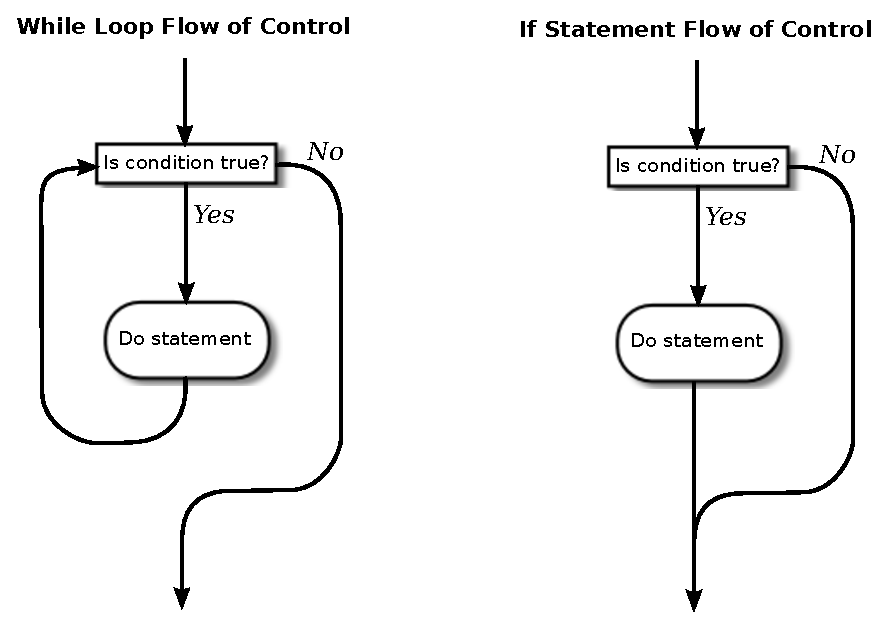
\includegraphics[scale=0.8]{images/while-and-if-flow-control.eps}
}

   
\noindent In these diagrams, the arrows represent the flow of time as the statement is executed.
Control enters the diagram at the top and leaves at the bottom.
Similarly, a flow control diagram for an \code{if..else} statement makes it clear
that exactly one of the two nested statements is executed:


\par\dumpfigure{
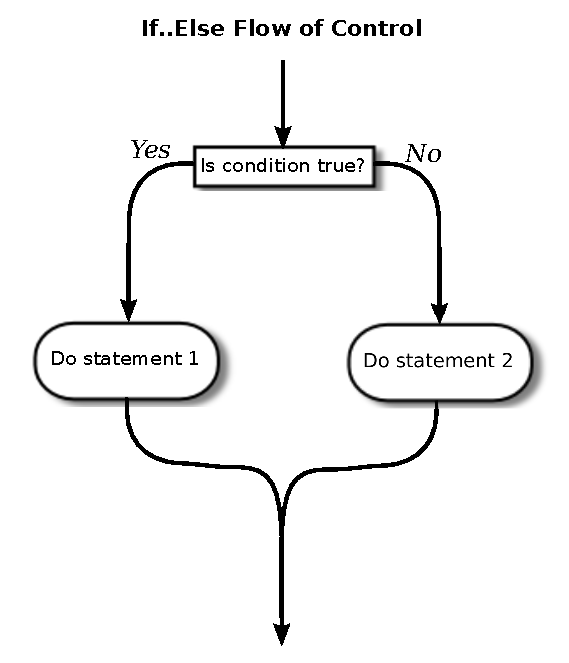
\includegraphics[scale=0.8]{images/if-else-flow-control.eps}
}

   

\mybreak



Of course, either or both of the \bnf{statements}
in an \code{if} statement can be a block, and again many programmers
prefer to add the braces even when they contain just a single statement.
So an \code{if} statement often looks like:

\displaycode{if ( \bnf{boolean-expression} ) \{
    \bnf{statements}
\}
else \{
    \bnf{statements}
\}}\donedisplaycode


\noindent or:

\displaycode{if ( \bnf{boolean-expression} ) \{
    \bnf{statements}
\}}\donedisplaycode



As an example, here is an \code{if} statement that exchanges the value of
two variables, \code{x} and \code{y}, but only if \code{x} is greater
than \code{y} to begin with. After this \code{if} statement has been
executed, we can be sure that the value of \code{x} is definitely less than
or equal to the value of \code{y}:

\displaycode{if ( x \> y ) \{
    int temp;      // A temporary variable for use in this block.
    temp = x;      // Save a copy of the value of x in temp.
    x = y;         // Copy the value of y into x.
    y = temp;      // Copy the value of temp into y.
\}}\donedisplaycode



Finally, here is an example of an \code{if} statement that includes an
\code{else} part. See if you can figure out what it does, and why it would be
used:

\displaycode{if ( years \> 1 ) \{  // handle case for 2 or more years
    System.out.print("The value of the investment after ");
    System.out.print(years);
    System.out.print(" years is \$");
\}
else \{  // handle case for 1 year
    System.out.print("The value of the investment after 1 year is \$");
\}  // end of if statement
System.out.printf("\%1.2f", principal);  // this is done in any case}\donedisplaycode




I'll have more to say about control structures later in this chapter. But
you already know the essentials. If you never learned anything more about
control structures, you would already know enough to perform any possible
computing task. Simple looping and branching are all you really need!



\subsection{Definite Assignment}\label{control.1.4}



I will finish this introduction to control structures with a somewhat technical
issue that you might not fully understand the first time you encounter it.
Consider the following two code segments, which seem to be entirely equivalent:

\displaycode{int y;                          int y;
if (x \< 0) \{                    if (x \< 0) \{
    y = 1;                           y = 1;
\}                               \}
else \{                          if (x \>= 0) \{
    y = 2;                           y = 2;
\}                               \}
System.out.println(y);          System.out.println(y);}\donedisplaycode


\noindent In the version on the left, \code{y} is assigned the value 1 if \code{x~\<~0}
and is assigned the value 2 otherwise, that is, if \code{x~\>=~0}.  Exactly the same is true of the
version on the right.  However, there is a subtle difference.  In fact, the Java compiler will report
an error for the \code{System.out.println} statement in the code on the right, while the
code on the left is perfectly fine!  



The problem is that in the code on the right, the computer can't tell that the
variable \code{y} has definitely been assigned a value.  When an \code{if}
statement has no \code{else} part, the statement inside the \code{if}
might or might not be executed, depending on the value of the condition.  The compiler can't
tell whether it will be executed or not, since the condition will only be evaluated when
the program is running.  For the code on the right above, as far as the compiler is concerned,
it is possible that \textbf{neither} statement, \code{y~=~1} or \code{y~=~2},
will be evaluated, so it is possible that the output statement is trying to print an undefined value.
The compiler considers this to be an error.  The value of a variable can only be used if the
compiler can \textbf{verify} that the variable will have been assigned a value at that point when the
program is running.  This is called \newword{definite assignment}.  (It doesn't matter
that \textbf{you} can tell that \code{y} will always be assigned a value in this example.
The question is whether the compiler can tell.)


Note that in the code on the left above, \code{y} is definitely assigned a value,
since in an \code{if..else} statement, one of the two alternatives will be executed
no matter what the value of the condition in the \code{if}.  
It is important that you understand that there is a 
difference between an \code{if..else} statement and a pair of plain \code{if} statements.
Here is another pair of code segments that might seem to do the same thing,
but don't.  What's the value of \code{x} after each code segment is executed?

\displaycode{
int x;                             int x;
x = -1;                            x = -1;
if (x \< 0)                         if (x \< 0)
    x = 1;                             x = 1;
else                               if (x \>= 0)
    x = 2;                             x = 2;
}\donedisplaycode


\noindent After the code on the left is executed, \code{x} is 1; after the code on the
right, \code{x} is~2.





   



\section{Algorithm Development}\label{control.2}



\start{{\Large P}rogramming is difficult} (like many activities that
are useful and worthwhile---and like most of those activities, it can also be
rewarding and a lot of fun). When you write a program, you have to tell the
computer every small detail of what to do. And you have to get everything
exactly right, since the computer will blindly follow your program exactly as
written. How, then, do people write any but the most simple programs? It's not
a big mystery, actually. It's a matter of learning to think in the right
way.


A program is an expression of an idea. A programmer starts with a general
idea of a task for the computer to perform. Presumably, the programmer has some
idea of how to perform the task by hand, at least in general outline. The
problem is to flesh out that outline into a complete, unambiguous, step-by-step
procedure for carrying out the task. Such a procedure is called an ``algorithm."
(Technically, an \newword{algorithm} is an unambiguous,
step-by-step procedure that always terminates after a finite number of steps. We don't
want to count procedures that might go on forever.) An algorithm is not the same as a
program. A program is written in some particular programming language. An
algorithm is more like the \textbf{idea} behind the program, but it's the idea of
the \textbf{steps} the program will take to perform its task, not just the idea
of the \textbf{task} itself. When describing an algorithm, the steps 
don't necessarily have to be specified in complete detail, 
as long as the steps are unambiguous and it's clear that
carrying out the steps will accomplish the assigned task. An algorithm can be
expressed in any language, including English. Of course, an algorithm can only
be expressed as an actual program if all the details have been filled in.


So, where do algorithms come from? Usually, they have to be developed, often
with a lot of thought and hard work. Skill at algorithm development is
something that comes with practice, but there are techniques and guidelines
that can help. I'll talk here about some techniques and guidelines that are
relevant to ``programming in the small," and I will return to the subject
several times in later chapters.

\subsection{Pseudocode and Stepwise Refinement}\label{control.2.1}



When programming in the small, you have a few basics to work with:
variables, assignment statements, and input/output routines. You might also
have some subroutines, objects, or other building blocks that have already been
written by you or someone else. (Input/output routines fall into this class.)
You can build sequences of these basic instructions, and you can also combine
them into more complex control structures such as \code{while} loops and
\code{if} statements.


Suppose you have a task in mind that you want the computer to perform. One
way to proceed is to write a description of the task, and take that description
as an outline of the algorithm you want to develop. Then you can refine and
elaborate that description, gradually adding steps and detail, until you have a
complete algorithm that can be translated directly into programming language.
This method is called \newword{stepwise refinement}, and it
is a type of top-down design. As you proceed through the stages of stepwise
refinement, you can write out descriptions of your algorithm in 
\newword{pseudocode}---informal instructions that imitate the structure
of programming languages without the complete detail and perfect syntax of
actual program code.


As an example, let's see how one might develop the program from the previous
section, which computes the value of an investment over five years. The task
that you want the program to perform is: ``Compute and display the value of an
investment for each of the next five years, where the initial investment and
interest rate are to be specified by the user." You might then write---or more likely
just think---that this can be expanded as:

\displaycode{Get the user's input
Compute the value of the investment after 1 year
Display the value
Compute the value after 2 years
Display the value
Compute the value after 3 years
Display the value
Compute the value after 4 years
Display the value
Compute the value after 5 years
Display the value}\donedisplaycode



This is correct, but rather repetitive. And seeing that repetition, you
might notice an opportunity to use a loop. A loop would take less typing. More
important, it would be more \textbf{general}: Essentially the same loop
will work no matter how many years you want to process. So, you might rewrite
the above sequence of steps as:

\displaycode{Get the user's input
while there are more years to process:
    Compute the value after the next year
    Display the value}\donedisplaycode



Following this algorithm would certainly solve the problem, but
for a computer we'll have to be more explicit about how to ``Get the
user's input," how to ``Compute the value after the next year," and what it
means to say ``there are more years to process." We can expand the step, ``Get
the user's input" into

\displaycode{Ask the user for the initial investment
Read the user's response
Ask the user for the interest rate
Read the user's response}\donedisplaycode



To fill in the details of the step ``Compute the value after the next year,"
you have to know how to do the computation yourself. (Maybe you need to ask
your boss or professor for clarification?) Let's say you know that the value is
computed by adding some interest to the previous value. Then we can refine the
\code{while} loop to:

\displaycode{while there are more years to process:
    Compute the interest
    Add the interest to the value
    Display the value}\donedisplaycode



As for testing whether there are more years to process, the only way that we
can do that is by counting the years ourselves. This displays a very common
pattern, and you should expect to use something similar in a lot of programs:
We have to start with zero years, add one each time we process a year, and stop
when we reach the desired number of years.  This is sometimes called a \newword{counting loop}.
So the \code{while} loop
becomes:

\displaycode{years = 0
while years \< 5:
    years = years + 1
    Compute the interest
    Add the interest to the value
    Display the value}\donedisplaycode



We still have to know how to compute the interest. Let's say that the
interest is to be computed by multiplying the interest rate by the current
value of the investment. Putting this together with the part of the algorithm
that gets the user's inputs, we have the complete algorithm:

\displaycode{Ask the user for the initial investment
Read the user's response
Ask the user for the interest rate
Read the user's response
years = 0
while years \< 5:
    years = years + 1
    Compute interest = value * interest rate
    Add the interest to the value
    Display the value}\donedisplaycode



Finally, we are at the point where we can translate pretty directly into
proper programming-language syntax. We still have to choose names for the
variables, decide exactly what we want to say to the user, and so forth. Having
done this, we could express our algorithm in Java as:

\displaycode{double principal, rate, interest;  // declare the variables
int years;
System.out.print("Type initial investment: ");
principal = TextIO.getlnDouble();
System.out.print("Type interest rate: ");
rate = TextIO.getlnDouble();
years = 0;
while (years \< 5) \{
   years = years + 1;
   interest = principal * rate;
   principal = principal + interest;
   System.out.println(principal);
\}}\donedisplaycode



This still needs to be wrapped inside a complete program, it still needs to
be commented, and it really needs to print out more information in a nicer format for the user.
But it's essentially the same program as the one in the previous section. (Note
that the pseudocode algorithm used indentation to show which statements are
inside the loop. In Java, indentation is completely ignored by the computer, so
you need a pair of braces to tell the computer which statements are in the
loop. If you leave out the braces, the only statement inside the loop would be
``\code{years~=~years~+~1;"}. The other statements would only be executed
once, after the loop ends. The nasty thing is that the computer won't notice
this error for you, like it would if you left out the parentheses around
``\code{(years~\<~5)}". The parentheses are required by the syntax of the
\code{while} statement. The braces are only required semantically. The
computer can recognize syntax errors but not semantic errors.)


One thing you should have noticed here is that my original specification of
the problem---``Compute and display the value of an investment for each of the
next five years"---was far from being complete. Before you start writing a
program, you should make sure you have a complete specification of exactly what
the program is supposed to do. In particular, you need to know what information
the program is going to input and output and what computation it is going to
perform. Here is what a reasonably complete specification of the problem might
look like in this example:


\medbreak
{\advance \leftskip by 70 pt \advance \rightskip by 70 pt




``Write a program that will compute and display the value of an investment
for each of the next five years. Each year, interest is added to the value. The
interest is computed by multiplying the current value by a fixed interest rate.
Assume that the initial value and the rate of interest are to be input by the
user when the program is run."


}
\medbreak



\subsection{The 3N+1 Problem}\label{control.2.2}



Let's do another example, working this time with a program that you haven't
already seen. The assignment here is an abstract mathematical problem that is
one of my favorite programming exercises. This time, we'll start with a more
complete specification of the task to be performed:


\medbreak
{\advance \leftskip by 70 pt \advance \rightskip by 70 pt




``Given a positive integer, N, define the '3N+1' sequence starting from N as
follows: If N is an even number, then divide N by two; but if N is odd, then
multiply N by 3 and add 1. Continue to generate numbers in this way until N
becomes equal to 1. For example, starting from N = 3, which is odd, we multiply
by 3 and add 1, giving N = 3*3+1 = 10. Then, since N is even, we divide by 2,
giving N = 10/2 = 5. We continue in this way, stopping when we reach 1.
The complete sequence is: 3, 10, 5, 16, 8, 4, 2, 1.


``Write a program that will read a positive integer from the user and will
print out the 3N+1 sequence starting from that integer. The program should also
count and print out the number of terms in the sequence."


}
\medbreak


\noindent A general outline of the algorithm for the program we want is:

\displaycode{   Get a positive integer N from the user.
   Compute, print, and count each number in the sequence.
   Output the number of terms.}\donedisplaycode



The bulk of the program is in the second step. We'll need a loop, since we
want to keep computing numbers until we get 1. To put this in terms appropriate
for a \code{while} loop, we need to know when to \textbf{continue} the
loop rather than when to stop it: We want to continue as long as the number is
\textbf{not} 1. So, we can expand our pseudocode algorithm to:

\displaycode{Get a positive integer N from the user;
while N is not 1:
    Compute N = next term;
    Output N;
    Count this term;
Output the number of terms;}\donedisplaycode



In order to compute the next term, the computer must take different actions
depending on whether N is even or odd. We need an \code{if} statement to
decide between the two cases:

\displaycode{Get a positive integer N from the user;
while N is not 1:
    if N is even:
       Compute N = N/2;
    else
       Compute N = 3 * N + 1;
    Output N;
    Count this term;
Output the number of terms;}\donedisplaycode



We are almost there. The one problem that remains is counting. Counting
means that you start with zero, and every time you have something to count, you
add one. We need a variable to do the counting. The variable must be set
to zero once, \textbf{before} the loop starts, and it must be incremented
within the loop.  (Again, this is a common
pattern that you should expect to see over and over.) With the counter added,
we get:

\displaycode{Get a positive integer N from the user;
Let counter = 0;
while N is not 1:
    if N is even:
       Compute N = N/2;
    else
       Compute N = 3 * N + 1;
    Output N;
    Add 1 to counter;
Output the counter;}\donedisplaycode



We still have to worry about the very first step. How can we get a
\textbf{positive} integer from the user? If we just read in a number,
it's possible that the user might type in a negative number or zero. If you
follow what happens when the value of N is negative or zero, you'll see that
the program will go on forever, since the value of N will never become equal to
1. This is bad. In this case, the problem is probably no big deal, but in
general you should try to write programs that are foolproof. One way to fix
this is to keep reading in numbers until the user types in a positive
number:

\displaycode{Ask user to input a positive number;
Let N be the user's response;
while N is not positive:
   Print an error message;
   Read another value for N;
Let counter = 0;
while N is not 1:
    if N is even:
       Compute N = N/2;
    else
       Compute N = 3 * N + 1;
    Output N;
    Add 1 to counter;
Output the counter;}\donedisplaycode



The first \code{while} loop will end only when N is a positive number, as
required. (A common beginning programmer's error is to use an \code{if}
statement instead of a \code{while} statement here: ``If N is not positive,
ask the user to input another value." The problem arises if the second number
input by the user is also non-positive. The \code{if} statement is only
executed once, so the second input number is never tested, and the program
proceeds into an infinite loop. With the
\code{while} loop, after the second number is input, the computer jumps back
to the beginning of the loop and tests whether the second number is positive.
If not, it asks the user for a third number, and it will continue asking for
numbers until the user enters an acceptable input.  After the while loop ends, we
can be absolutely sure that \code{N} is a positive number.)


Here is a Java program implementing this algorithm. It uses the operators
\code{\<=} to mean ``is less than or equal to" and \code{!=} to mean ``is
not equal to." To test whether N is even, it uses ``\code{N~\%~2~==~0}". All
the operators used here were discussed in Section~\ref{basics.5}.

\displaycode{/**  
 * This program prints out a 3N+1 sequence starting from a positive 
 * integer specified by the user.  It also counts the number of 
 * terms in the sequence, and prints out that number.
 */
 public class ThreeN1 \{
 
      public static void main(String[] args) \{                
        
         int N;       // for computing terms in the sequence
         int counter; // for counting the terms
        
         System.out.print("Starting point for sequence: ");
         N = TextIO.getlnInt();
         while (N \<= 0) \{
            System.out.print(
                   "The starting point must be positive. Please try again: " );
            N = TextIO.getlnInt();
         \}
         // At this point, we know that N \> 0
        
         counter = 0;
         while (N != 1) \{
             if (N \% 2 == 0)
                N = N / 2;
             else
                N = 3 * N + 1;
             System.out.println(N);
             counter = counter + 1;
         \}
        
         System.out.println();
         System.out.print("There were ");
         System.out.print(counter);
         System.out.println(" terms in the sequence.");
                           
     \}  // end of main()
 
 \}  // end of class ThreeN1}\donedisplaycode




Two final notes on this program: First, you might have noticed that the
first term of the sequence---the value of N input by the user---is not
printed or counted by this program. Is this an error? It's hard to say. Was the
specification of the program careful enough to decide? This is the type of
thing that might send you back to the boss/professor for clarification. The
problem (if it is one!) can be fixed easily enough. Just replace the line
``counter = 0" before the while loop with the two lines:

\displaycode{System.out.println(N);   // print out initial term
counter = 1;       // and count it}\donedisplaycode



Second, there is the question of why this problem might be interesting.
Well, it's interesting to mathematicians and computer scientists because of a
simple question about the problem that they haven't been able to answer: Will
the process of computing the 3N+1 sequence finish after a finite number of
steps for all possible starting values of N? Although individual sequences are
easy to compute, no one has been able to answer the general question. To put
this another way, no one knows whether the process of computing 3N+1 sequences
can properly be called an algorithm, since an algorithm is required to
terminate after a finite number of steps!  (Note: This discussion 
really applies to integers, not to values of type \ptype{int}!  That is, it
assumes that
the value of \code{N} can take on arbitrarily large integer values, which
is not true for a variable of type \ptype{int} in a Java program.
When the value of \code{N} in the program becomes too large to be
represented as a 32-bit \ptype{int}, the values output by the program
are no longer mathematically correct.  So the Java program does not compute
the correct 3N+1 sequence if \code{N} becomes too large.  See Exercise~8.2.)



   
\subsection{Coding, Testing, Debugging}\label{control.2.3}




It would be nice if, having developed an algorithm for your program, you
could relax, press a button, and get a perfectly working program.
Unfortunately, the process of turning an algorithm into Java source code
doesn't always go smoothly. And when you do get to the stage of a working
program, it's often only working in the sense that it does \textbf{something}.
Unfortunately not what you want it to do.


After program design comes coding: translating the design into a program
written in Java or some other language. Usually, no matter how careful you are,
a few syntax errors will creep in from somewhere, and the Java compiler will
reject your program with some kind of error message. Unfortunately, while a
compiler will always detect syntax errors, it's not very good about telling you
exactly what's wrong. Sometimes, it's not even good about telling you where the
real error is. A spelling error or missing ``\{" on line 45 might cause the
compiler to choke on line 105. You can avoid lots of errors by making sure that
you really understand the syntax rules of the language and by following some
basic programming guidelines. For example, I never type a ``\{" without typing
the matching ``\}". Then I go back and fill in the statements between the braces.
A missing or extra brace can be one of the hardest errors to find in a large
program. Always, always indent your program nicely. If you change the program,
change the indentation to match. It's worth the trouble. Use a consistent
naming scheme, so you don't have to struggle to remember whether you called
that variable \code{interestrate} or \code{interestRate}. In general, when
the compiler gives multiple error messages, don't try to fix the second error
message from the compiler until you've fixed the first one. Once the compiler
hits an error in your program, it can get confused, and the rest of the error
messages might just be guesses. Maybe the best advice is: Take the time to
understand the error before you try to fix it. Programming is not an
experimental science.


When your program compiles without error, you are still not done. You have
to test the program to make sure it works correctly. Remember that the goal is
not to get the right output for the two sample inputs that the professor gave
in class. The goal is a program that will work correctly for all reasonable
inputs. Ideally, when faced with an unreasonable input, it should respond by
gently chiding the user rather than by crashing. Test your program on a wide
variety of inputs. Try to find a set of inputs that will test the full range of
functionality that you've coded into your program. As you begin writing larger
programs, write them in stages and test each stage along the way. You might
even have to write some extra code to do the testing---for example to call a
subroutine that you've just written. You don't want to be faced, if you can
avoid it, with 500 newly written lines of code that have an error in there
\textit{somewhere.}


The point of testing is to find \newword{bugs}---semantic 
errors that show up as incorrect behavior rather than as compilation
errors. And the sad fact is that you will probably find them. Again, you can
minimize bugs by careful design and careful coding, but no one has found a way
to avoid them altogether. Once you've detected a bug, it's time for
\newword{debugging}. You have to track down the cause of the
bug in the program's source code and eliminate it. Debugging is a skill that,
like other aspects of programming, requires practice to master. So don't be
afraid of bugs. Learn from them. One essential debugging skill is the ability
to read source code---the ability to put aside preconceptions about what you
\textit{think} it does and to follow it the way the computer does---mechanically, 
step-by-step---to see what it really does. This is hard. I can
still remember the time I spent hours looking for a bug only to find that a
line of code that I had looked at ten times had a ``1" where it should have had
an ``i", or the time when I wrote a subroutine named \code{WindowClosing}
which would have done exactly what I wanted except that the computer was
looking for \code{windowClosing} (with a lower case ``w"). Sometimes it can
help to have someone who doesn't share your preconceptions look at your
code.


Often, it's a problem just to find the part of the program that contains the
error. Most programming environments come with a \newword{debugger}, 
which is a program that can help you find bugs.
Typically, your program can be run under the control of the debugger. The
debugger allows you to set ``breakpoints" in your program. A breakpoint is a
point in the program where the debugger will pause the program so you can look
at the values of the program's variables. The idea is to track down exactly
when things start to go wrong during the program's execution. The debugger will
also let you execute your program one line at a time, so that you can watch
what happens in detail once you know the general area in the program where the
bug is lurking.


I will confess that I only occasionally use debuggers myself. A more traditional
approach to debugging is to insert \newword{debugging statements} into your program. 
These are output statements that print out
information about the state of the program. Typically, a debugging statement
would say something like

\displaycode{System.out.println("At start of while loop, N = " + N);}\donedisplaycode
 

\noindent You need to be able to tell from the output where in your program the output is
coming from, and you want to know the value of important variables. Sometimes,
you will find that the computer isn't even getting to a part of the program
that you think it should be executing. Remember that the goal is to find the
first point in the program where the state is not what you expect it to be.
That's where the bug is.


And finally, remember the golden rule of debugging: If you are absolutely
sure that everything in your program is right, and if it still doesn't work,
then one of the things that you are absolutely sure of is wrong.
   

   

   



\section[while and do..while]{The while and do..while Statements}\label{control.3}



\start{{\Large S}tatements in Java can} be either simple statements
or compound statements. Simple statements, such as assignment statements and
subroutine call statements, are the basic building blocks of a program.
Compound statements, such as \code{while} loops and \code{if} statements,
are used to organize simple statements into complex structures, which are
called control structures because they control the order in which the
statements are executed. The next five sections explore the details of
control structures that are available in Java, starting with the \code{while}
statement and the \code{do..while} statement in this section. At the same
time, we'll look at examples of programming with each control structure and
apply the techniques for designing algorithms that were introduced in the
previous~section.


\subsection{The while Statement}\label{control.3.1}



The \code{while} statement was already introduced in Section~\ref{control.1}. 
A \code{while} loop has the form

\displaycode{while ( \bnf{boolean-expression} )
   \bnf{statement}}\donedisplaycode


\noindent The \bnf{statement} can, of course, be a block
statement consisting of several statements grouped together between a pair of
braces. This statement is called the \newword{body of the loop}. 
The body of the loop is repeated as long as the \bnf{boolean-expression} is true. This boolean expression is
called the \newword{continuation condition}, or more simply
the \newword{test}, of the loop. There are a few points that
might need some clarification. What happens if the condition is false in the
first place, before the body of the loop is executed even once? In that case,
the body of the loop is never executed at all. The body of a while loop can be
executed any number of times, including zero. What happens if the condition is
true, but it becomes false somewhere in the \textbf{middle} of the loop
body? Does the loop end as soon as this happens? It doesn't, because the
computer continues executing the body of the loop until it gets to the end.
Only then does it jump back to the beginning of the loop and test the
condition, and only then can the loop end.


Let's look at a typical problem that can be solved using a \code{while}
loop: finding the average of a set of positive integers entered by the user.
The average is the sum of the integers, divided by the number of integers. The
program will ask the user to enter one integer at a time. It will keep count of
the number of integers entered, and it will keep a running total of all the
numbers it has read so far. Here is a pseudocode algorithm for the program:

\displaycode{Let sum = 0     // The sum of the integers entered by the user.
Let count = 0   // The number of integers entered by the user.
while there are more integers to process:
    Read an integer
    Add it to the sum
    Count it
Divide sum by count to get the average
Print out the average}\donedisplaycode



But how can we test whether there are more integers to process? A typical
solution is to tell the user to type in zero after all the data have been
entered. This will work because we are assuming that all the data are positive
numbers, so zero is not a legal data value. The zero is not itself part of the
data to be averaged. It's just there to mark the end of the real data. A data
value used in this way is sometimes called a \newword{sentinel value}. 
So now the test in the while loop becomes ``while the input
integer is not zero". But there is another problem! The first time the test is
evaluated, before the body of the loop has ever been executed, no integer has
yet been read. There is no ``input integer" yet, so testing whether the input
integer is zero doesn't make sense. So, we have to do something
\textbf{before} the while loop to make sure that the test makes sense.
Setting things up so that the test in a \code{while} loop makes sense the
first time it is executed is called \newword{priming the loop}. 
In this case, we can simply read the first integer before the
beginning of the loop. Here is a revised algorithm:

\displaycode{Let sum = 0
Let count = 0
Read an integer
while the integer is not zero:
    Add the integer to the sum
    Count it
    Read an integer
Divide sum by count to get the average
Print out the average}\donedisplaycode



Notice that I've rearranged the body of the loop. Since an integer is read
before the loop, the loop has to begin by processing that integer. At the end
of the loop, the computer reads a new integer. The computer then jumps back to
the beginning of the loop and tests the integer that it has just read. Note
that when the computer finally reads the sentinel value, the loop ends before
the sentinel value is processed. It is not added to the sum, and it is not
counted. This is the way it's supposed to work. The sentinel is not part of the
data. The original algorithm, even if it could have been made to work without
priming, was incorrect since it would have summed and counted all the integers,
including the sentinel. (Since the sentinel is zero, the sum would still be
correct, but the count would be off by one. Such so-called \newword{off-by-one errors} 
are very common. Counting turns out to be
harder than it looks!)


We can easily turn the algorithm into a complete program. Note that the
program cannot use the statement ``\code{average~=~sum/count};" to compute the
average. Since \code{sum} and \code{count} are both variables of type
\ptype{int}, the value of \code{sum/count} is an integer. The average should
be a real number. We've seen this problem before: we have to convert one of the
\ptype{int} values to a \ptype{double} to force the computer to compute the
quotient as a real number. This can be done by type-casting one of the
variables to type \ptype{double}. The type cast ``(double)sum" converts the
value of \code{sum} to a real number, so in the program the average is
computed as ``\code{average~= ((double)sum)~/~count};". Another solution in
this case would have been to declare \code{sum} to be a variable of type
\ptype{double} in the first place.


One other issue is addressed by the program: If the user enters zero as the
first input value, there are no data to process. We can test for this case by
checking whether \code{count} is still equal to zero after the \code{while}
loop. This might seem like a minor point, but a careful programmer should cover
all the bases.



Here is the full source code for the program:

\displaycode{/**
 * This program reads a sequence of positive integers input
 * by the user, and it will print out the average of those
 * integers.  The user is prompted to enter one integer at a
 * time.  The user must enter a 0 to mark the end of the
 * data.  (The zero is not counted as part of the data to
 * be averaged.)  The program does not check whether the
 * user's input is positive, so it will actually add up
 * both positive and negative input values.
 */

public class ComputeAverage \{
        
   public static void main(String[] args) \{
      
      int inputNumber;   // One of the integers input by the user.
      int sum;           // The sum of the positive integers.
      int count;         // The number of positive integers.
      double average;    // The average of the positive integers.
      
      /* Initialize the summation and counting variables. */
      
      sum = 0;
      count = 0;
      
      /* Read and process the user's input. */
      
      System.out.print("Enter your first positive integer: ");
      inputNumber = TextIO.getlnInt();
      
      while (inputNumber != 0) \{
         sum += inputNumber;   // Add inputNumber to running sum.
         count++;              // Count the input by adding 1 to count.
         System.out.print("Enter your next positive integer, or 0 to end: ");
         inputNumber = TextIO.getlnInt();
      \}
      
      /* Display the result. */
      
      if (count == 0) \{
         System.out.println("You didn't enter any data!");
      \}
      else \{
         average = ((double)sum) / count;
         System.out.println();
         System.out.println("You entered " + count + " positive integers.");
         System.out.printf("Their average is \%1.3f.\1n", average);
      \}
 
   \} // end main()
   
\} // end class ComputeAverage}\donedisplaycode



   
\subsection{The do..while Statement}\label{control.3.2}

   


Sometimes it is more convenient to test the continuation condition at the
end of a loop, instead of at the beginning, as is done in the \code{while}
loop. The \code{do..while} statement is very similar to the \code{while}
statement, except that the word ``while," along with the condition that it
tests, has been moved to the end. The word ``do" is added to mark the beginning
of the loop. A \code{do..while} statement has the form

\displaycode{do
    \bnf{statement}
while ( \bnf{boolean-expression} );}\donedisplaycode


\noindent or, since, as usual, the \bnf{statement} can be a
block,

\displaycode{do \{
    \bnf{statements}
\} while ( \bnf{boolean-expression} );}\donedisplaycode


\noindent Note the semicolon, ';', at the very  end. This semicolon is part of the
statement, just as the semicolon at the end of an assignment statement or
declaration is part of the statement. Omitting it is a syntax error. (More
generally, \textbf{every} statement in Java ends either with a
semicolon or a right brace, '\}'.)


To execute a \code{do} loop, the computer first executes the body of the
loop---that is, the statement or statements inside the loop---and then it
evaluates the boolean expression. If the value of the expression is
\code{true}, the computer returns to the beginning of the \code{do} loop and repeats
the process; if the value is \code{false}, it ends the loop and continues
with the next part of the program. Since the condition is not tested until the
end of the loop, the body of a \code{do} loop is always executed at least once.


For example, consider the following pseudocode for a game-playing program.
The \code{do} loop makes sense here instead of a \code{while} loop because
with the \code{do} loop, you know there will be at least one game. Also, the
test that is used at the end of the loop wouldn't even make sense at the
beginning:

\displaycode{do \{
   Play a Game
   Ask user if he wants to play another game
   Read the user's response
\} while ( the user's response is yes );}\donedisplaycode



Let's convert this into proper Java code. Since I don't want to talk about
game playing at the moment, let's say that we have a class named
\code{Checkers}, and that the \code{Checkers} class contains a static
member subroutine named \code{playGame()} that plays one game of checkers
against the user. Then, the pseudocode ``Play a game" can be expressed as the
subroutine call statement ``\code{Checkers.playGame();}". We need a variable
to store the user's response. The \classname{TextIO} class makes it convenient to
use a \ptype{boolean} variable to store the answer to a yes/no question. The
input function \code{TextIO.getlnBoolean()} allows the user to enter the
value as ``yes" or ``no" (among other acceptable responses). 
``Yes" is considered to be \code{true}, and ``no" is
considered to be \code{false}. So, the algorithm can be coded as

\displaycode{boolean wantsToContinue;  // True if user wants to play again.
do \{
   Checkers.playGame();
   System.out.print("Do you want to play again? ");
   wantsToContinue = TextIO.getlnBoolean();
\} while (wantsToContinue == true);}\donedisplaycode


\noindent When the value of the \ptype{boolean} variable is set to \code{false}, it
is a signal that the loop should end. When a \ptype{boolean} variable is used
in this way---as a signal that is set in one part of the program and tested in
another part---it is sometimes called a \newword{flag} or
\newword{flag variable} (in the sense of a signal flag).


By the way, a more-than-usually-pedantic programmer would sneer at the test
``\code{while (wantsToContinue == true)}". This test is exactly equivalent to
``\code{while (wantsToContinue)}". Testing whether ``\code{wantsToContinue~==~true}" 
is true amounts to the same thing as testing whether
``\code{wantsToContinue}" is true. A little less offensive is an expression of
the form ``\code{flag~==~false}", where \code{flag} is a boolean variable.
The value of ``\code{flag~==~false}" is exactly the same as the value of
``\code{!flag}", where \code{!} is the boolean negation operator. So you can
write ``\code{while~(!flag)}" instead of ``\code{while (flag~==~false)}", and
you can write ``\code{if~(!flag)}" instead of ``\code{if~(flag~==~false)}".


Although a \code{do..while} statement is sometimes more convenient than a
\code{while} statement, having two kinds of loops does not make the language
more powerful. Any problem that can be solved using \code{do..while} loops
can also be solved using only \code{while} statements, and vice versa. In
fact, if \bnf{doSomething} represents any block of
program code, then

\displaycode{do \{
    \bnf{doSomething}
\} while ( \bnf{boolean-expression} );}\donedisplaycode


\noindent has exactly the same effect as

\displaycode{\bnf{doSomething}
while ( \bnf{boolean-expression} ) \{
    \bnf{doSomething}
\}}\donedisplaycode


\noindent Similarly,

\displaycode{while ( \bnf{boolean-expression} ) \{
    \bnf{doSomething}
\} }\donedisplaycode


\noindent can be replaced by

\displaycode{if ( \bnf{boolean-expression} ) \{
   do \{
       \bnf{doSomething}
   \} while ( \bnf{boolean-expression} );
\}}\donedisplaycode


\noindent without changing the meaning of the program in any way.



   
\subsection{break and continue}\label{control.3.3}



The syntax of the \code{while} and \code{do..while} loops allows you to
test the continuation condition at either the beginning of a loop or at the
end. Sometimes, it is more natural to have the test in the middle of the loop,
or to have several tests at different places in the same loop. Java provides a
general method for breaking out of the middle of any loop. It's called the
\code{break} statement, which takes the form

\displaycode{break;}\donedisplaycode



When the computer executes a \code{break} statement in a loop, it will
immediately jump out of the loop. It then continues on to whatever follows the
loop in the program. Consider for example:

\displaycode{while (true) \{  // looks like it will run forever!
   System.out.print("Enter a positive number: ");
   N = TextIO.getlnInt();
   if (N \> 0)   // the input value is OK, so jump out of loop
      break;
   System.out.println("Your answer must be \> 0.");
\}
// continue here after break}\donedisplaycode


\noindent If the number entered by the user is greater than zero, the \code{break}
statement will be executed and the computer will jump out of the loop.
Otherwise, the computer will print out ``Your answer must be \> 0." and will
jump back to the start of the loop to read another input value.


The first line of this loop, ``\code{while~(true)}" might look a bit
strange, but it's perfectly legitimate. The condition in a \code{while} loop
can be any boolean-valued expression. The computer evaluates this expression
and checks whether the value is \code{true} or \code{false}. The boolean
literal ``\code{true}" is just a boolean expression that always evaluates to
true. So ``\code{while~(true)}" can be used to write an infinite loop, or one
that will be terminated by a \code{break} statement.


A \code{break} statement terminates the loop that immediately encloses the
\code{break} statement. It is possible to have \newword{nested} loops, 
where one loop statement is contained inside
another. If you use a \code{break} statement inside a nested loop, it will
only break out of that loop, not out of the loop that contains the nested loop. 
There is something called a \newword{labeled break} statement that allows you to
specify which loop you want to break. This is not very common, so I will go over it quickly.
Labels work like this:  You can put a \newword{label} in
front of any loop.  A label consists of a simple identifier followed
by a colon.  For example, a \code{while} with a label might
look like ``\code{mainloop:~while\dots}".  Inside
this loop you can use the labeled break statement ``\code{break~mainloop;}"
to break out of the labeled loop.  For example, here is a code segment that checks
whether two strings, \code{s1} and \code{s2}, have a character in common.
If a common character is found, the value of the flag variable \code{nothingInCommon}
is set to \code{false}, and a labeled break is used to end the processing
at that point:

\displaycode{boolean nothingInCommon;
nothingInCommon = true;  // Assume s1 and s2 have no chars in common.
int i,j;  // Variables for iterating through the chars in s1 and s2.

i = 0;
bigloop: while (i \< s1.length()) \{
   j = 0;
   while (j \< s2.length()) \{
      if (s1.charAt(i) == s2.charAt(j)) \{ // s1 and s2 have a common char.
          nothingInCommon = false;
          break bigloop;  // break out of BOTH loops
      \}
      j++;  // Go on to the next char in s2.
   \}
   i++;  //Go on to the next char in s1.
\}}\donedisplaycode



\mybreak

   

The \code{continue} statement is related to \code{break}, but less
commonly used. A \code{continue} statement tells the computer to skip the
rest of the current iteration of the loop. However, instead of jumping out of
the loop altogether, it jumps back to the beginning of the loop and continues
with the next iteration (including evaluating the loop's continuation condition to
see whether any further iterations are required).  As with \code{break},
when a \code{continue} is in a nested loop, it will continue the loop
that directly contains it; a ``labeled continue" can be used to continue
the containing loop instead.


\code{break} and \code{continue} can be used in \code{while} loops and
\code{do..while} loops. They can also be used in \code{for} loops, which
are covered in the next~section. 
In Section~\ref{control.6}, we'll see that \code{break} can also be used to
break out of a \code{switch} statement.   A \code{break} can occur
inside an \code{if} statement, but only if the \code{if} statement
is nested inside a loop or inside a \code{switch} statement.
In that case, it does \textbf{not} mean
to break out of the \code{if}.  Instead, it breaks out of the loop or
\code{switch} statement that contains the \code{if} statement.
The same consideration applies to \code{continue} statements inside \code{ifs}.


   

   



\section{The for Statement}\label{control.4}

   

\start{{\Large W}e turn in this section} to another type of loop,
the \code{for} statement. Any \code{for} loop is equivalent to some
\code{while} loop, so the language doesn't get any additional power by having
\code{for} statements. But for a certain type of problem, a \code{for} loop
can be easier to construct and easier to read than the corresponding
\code{while} loop. It's quite possible that in real programs, \code{for}
loops actually outnumber \code{while} loops.

\subsection{For Loops}\label{control.4.1}



The \code{for} statement makes a common type of while loop easier to
write. Many while loops have the general form:

\displaycode{\bnf{initialization}
while ( \bnf{continuation-condition} ) \{
    \bnf{statements}
    \bnf{update}
\}}\donedisplaycode


\noindent For example, consider this example, copied from an example in Section~\ref{control.2}:

\displaycode{years = 0;  // \textbf{initialize} the variable years
while ( years \< 5 ) \{   // \textbf{condition} for continuing loop

    interest = principal * rate;    //
    principal += interest;          // do three \textbf{statements}
    System.out.println(principal);  //
    
    years++;   // \textbf{update} the value of the variable, years
\}}\donedisplaycode


\noindent This loop can be written as the following equivalent \code{for}
statement:

\displaycode{for ( years = 0;  years \< 5;  years++ ) \{
   interest = principal * rate;
   principal += interest;
   System.out.println(principal);
\}}\donedisplaycode


\noindent The initialization, continuation condition, and updating have all been
combined in the first line of the \code{for} loop. This keeps everything
involved in the ``control" of the loop in one place, which helps make the loop
easier to read and understand. The \code{for} loop is executed in exactly the
same way as the original code: The initialization part is executed once, before
the loop begins. The continuation condition is executed before each execution
of the loop, and the loop ends when this condition is \code{false}. The
update part is executed at the end of each execution of the loop, just before
jumping back to check the condition.


The formal syntax of the \code{for} statement is as follows:

\displaycode{for ( \bnf{initialization}; \bnf{continuation-condition}; \bnf{update} )
     \bnf{statement}}\donedisplaycode


\noindent or, using a block statement:

\displaycode{for ( \bnf{initialization}; \bnf{continuation-condition}; \bnf{update} ) \{
     \bnf{statements}
\}}\donedisplaycode


\noindent The \bnf{continuation-condition} must be a
boolean-valued expression. The \bnf{initialization}
is usually a declaration or an assignment statement, but it
can be any expression that would be allowed as a statement in a program.
The \bnf{update} can be any simple statement, but is usually
an increment, a decrement, or an assignment statement. Any
of the three parts can be empty. If the continuation condition is empty, it is
treated as if it were ``\code{true}," so the loop will be repeated forever or
until it ends for some other reason, such as a \code{break} statement. (Some
people like to begin an infinite loop with ``\code{for~(;;)}" instead of
``\code{while~(true)}".)  Here's a flow control diagram for a \code{for}
statement:


\par\dumpfigure{
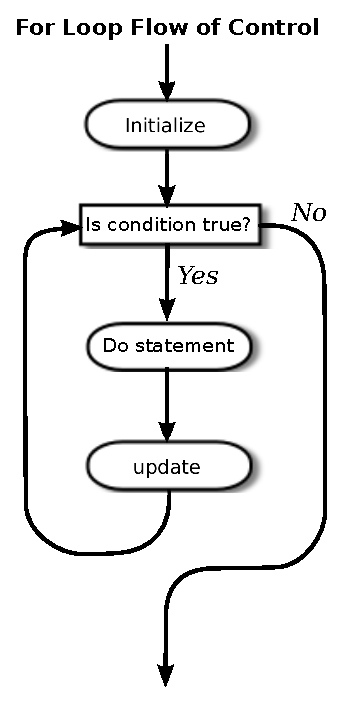
\includegraphics[scale=0.8]{images/for-loop-flow-control.eps}
}



Usually, the initialization part of a \code{for} statement assigns a value
to some variable, and the update changes the value of that variable with an
assignment statement or with an increment or decrement operation. The value of
the variable is tested in the continuation condition, and the loop ends when
this condition evaluates to \code{false}. A variable used in this way is
called a \newword{loop control variable}. In the
example given above, the loop control variable was \code{years}.


Certainly, the most common type of \code{for} loop is the \newword{counting loop}, 
where a loop control variable takes on all
integer values between some minimum and some maximum value. A counting loop has
the form

\displaycode{for ( \bnf{variable} = \bnf{min};  \bnf{variable} \<= \bnf{max}; \bnf{variable}++ ) \{
     \bnf{statements}
\}}\donedisplaycode


\noindent where \bnf{min} and \bnf{max} are integer-valued expressions (usually constants). The
\bnf{variable} takes on the values \bnf{min}, \bnf{min}+1, 
\bnf{min}+2,~\dots, \bnf{max}. The value
of the loop control variable is often used in the body of the loop. The
\code{for} loop at the beginning of this section is a counting loop in which
the loop control variable, \code{years}, takes on the values 1, 2, 3, 4, 5.
Here is an even simpler example, in which the numbers 1, 2,~\dots, 10 are
displayed on standard output:

\displaycode{for ( N = 1 ;  N \<= 10 ;  N++ )
   System.out.println( N );}\donedisplaycode


\noindent For various reasons, Java programmers like to start counting at 0 instead of
1, and they tend to use a ``\code{\<}" in the condition, rather than a
``\code{\<=}". The following variation of the above loop prints out the ten
numbers 0, 1, 2,~\dots, 9:

\displaycode{for ( N = 0 ;  N \< 10 ;  N++ )
   System.out.println( N );}\donedisplaycode


\noindent Using \code{\<} instead of \code{\<=} in the test, or vice versa, is
a common source of off-by-one errors in programs. You should always stop and
think, Do I want the final value to be processed or not?


It's easy to count down from 10 to 1 instead of counting up. Just start with
10, decrement the loop control variable instead of incrementing it, and
continue as long as the variable is greater than or equal to one.

\displaycode{for ( N = 10 ;  N \>= 1 ;  N-- )
   System.out.println( N );}\donedisplaycode



Now, in fact, the official syntax of a \code{for} statement actually
allows both the initialization part and the update part to consist of several
expressions, separated by commas. So we can even count up from 1 to 10 and
count down from 10 to 1 at the same time!

\displaycode{for ( i=1, j=10;  i \<= 10;  i++, j-- ) \{
   System.out.printf("\%5d", i); // Output i in a 5-character wide column.
   System.out.printf("\%5d", j); // Output j in a 5-character column 
   System.out.println();       //     and end the line.
\}}\donedisplaycode



As a final introductory example, let's say that we want to use a \code{for} loop that
prints out just the even numbers between 2 and 20, that is: 2, 4, 6, 8, 10, 12,
14, 16, 18, 20. There are several ways to do this. Just to show how even a very
simple problem can be solved in many ways, here are four different solutions
(three of which would get full credit):

\displaycode{ (1)   // There are 10 numbers to print.           
       // Use a for loop to count 1, 2,            
       // ..., 10.  The numbers we want            
       // to print are 2*1, 2*2, ... 2*10.         
   
       for (N = 1; N \<= 10; N++) \{              
          System.out.println( 2*N );                
       \}
       
       
 (2)   // Use a for loop that counts
       // 2, 4, ..., 20 directly by
       // adding 2 to N each time through
       // the loop.
       
       for (N = 2; N \<= 20; N = N + 2) \{
          System.out.println( N );
       \}
       
       
 (3)   // Count off all the numbers    
       // 2, 3, 4, ..., 19, 20, but                
       // only print out the numbers               
       // that are even.                           
    
       for (N = 2; N \<= 20; N++) \{               
          if ( N \% 2 == 0 ) // is N even?           
             System.out.println( N );               
       \} 
   
   
 (4)   // Irritate the professor with
       // a solution that follows the
       // letter of this silly assignment
       // while making fun of it.
       
       for (N = 1; N \<= 1; N++) \{
          System.out.println("2 4 6 8 10 12 14 16 18 20");
       \}
}\donedisplaycode


   

Perhaps it is worth stressing one more time that a \code{for} statement,
like any statement except for a variable declaration, never occurs on its own in a real program. A statement must
be inside the \code{main} routine of a program or inside some other
subroutine. And that subroutine must be defined inside a class. I should also
remind you that every variable must be declared before it can be used, and that
includes the loop control variable in a \code{for} statement. In all the
examples that you have seen so far in this section, the loop control variables
should be declared to be of type \ptype{int}. It is not required that a loop
control variable be an integer. Here, for example, is a \code{for} loop in
which the variable, \code{ch}, is of type \ptype{char}, using
the fact that the \code{++} operator can be applied to characters as
well as to numbers:

\displaycode{// Print out the alphabet on one line of output.
char ch;  // The loop control variable; 
          //       one of the letters to be printed.
for ( ch = 'A';  ch \<= 'Z';  ch++ )
    System.out.print(ch);
System.out.println();}\donedisplaycode

   

\subsection{Example: Counting Divisors}\label{control.4.2}



Let's look at a less trivial problem that can be solved with a \code{for}
loop. If \code{N} and \code{D} are positive integers, we say that
\code{D} is a \newword{divisor} of \code{N} if the
remainder when \code{D} is divided into \code{N} is zero. (Equivalently, we
could say that \code{N} is an even multiple of \code{D}.) In terms of Java
programming, \code{D} is a divisor of \code{N} if \code{N~\%~D} is
zero.


Let's write a program that inputs a positive integer, \code{N}, from the
user and computes how many different divisors \code{N} has. The numbers that
could possibly be divisors of \code{N} are 1, 2,~\dots,~\code{N}. To compute
the number of divisors of \code{N}, we can just test each possible divisor of
\code{N} and count the ones that actually do divide \code{N} evenly. In
pseudocode, the algorithm takes the form

\displaycode{Get a positive integer, N, from the user
Let divisorCount = 0
for each number, testDivisor, in the range from 1 to N:
    if testDivisor is a divisor of N:
        Count it by adding 1 to divisorCount
Output the count}\donedisplaycode


\noindent This algorithm displays a common programming pattern that is used when some,
but not all, of a sequence of items are to be processed. The general pattern
is

\displaycode{for each item in the sequence:
   if the item passes the test:
       process it}\donedisplaycode


\noindent The \code{for} loop in our divisor-counting algorithm can be translated
into Java code as

\displaycode{for (testDivisor = 1; testDivisor \<= N; testDivisor++) \{
   if ( N \% testDivisor == 0 )
      divisorCount++;
\}}\donedisplaycode



On a modern computer, this loop can be executed very quickly. It is not
impossible to run it even for the largest legal \ptype{int} value, 2147483647.
(If you wanted to run it for even larger values, you could use variables of
type \ptype{long} rather than \ptype{int}.) However, it does take a
significant amount of time for very large numbers. So when I implemented this
algorithm, I decided to output a dot every time the computer has tested one
million possible divisors. In the improved version of the program, there are
two types of counting going on. We have to count the number of divisors and we
also have to count the number of possible divisors that have been tested. So
the program needs two counters. When the second counter reaches 1000000, the program
outputs a '.' and resets the counter to zero so that we can start counting the
next group of one million. Reverting to pseudocode, the algorithm now looks
like

\displaycode{Get a positive integer, N, from the user
Let divisorCount = 0  // Number of divisors found.
Let numberTested = 0  // Number of possible divisors tested
                      //       since the last period was output.
for each number, testDivisor, in the range from 1 to N:
    if testDivisor is a divisor of N:
        Count it by adding 1 to divisorCount
    Add 1 to numberTested
    if numberTested is 1000000:
        print out a '.'
        Reset numberTested to 0
Output the count}\donedisplaycode


\noindent Finally, we can translate the algorithm into a complete Java program:

\displaycode{/**
 * This program reads a positive integer from the user.
 * It counts how many divisors that number has, and
 * then it prints the result.
 */
   
public class CountDivisors \{
   
   public static void main(String[] args) \{
      
      int N;  // A positive integer entered by the user.
              // Divisors of this number will be counted.
              
      int testDivisor;  // A number between 1 and N that is a
                        // possible divisor of N.
      
      int divisorCount;  // Number of divisors of N that have been found.
      
      int numberTested;  // Used to count how many possible divisors
                         // of N have been tested.  When the number
                         // reaches 1000000, a period is output and
                         // the value of numberTested is reset to zero.
                         
      /* Get a positive integer from the user. */
   
      while (true) \{
         System.out.print("Enter a positive integer: ");
         N = TextIO.getlnInt();
         if (N \> 0)
            break;
         System.out.println("That number is not positive.  Please try again.");
      \}
      
      /* Count the divisors, printing a "." after every 1000000 tests. */
    
      divisorCount = 0;
      numberTested = 0;
      
      for (testDivisor = 1; testDivisor \<= N; testDivisor++) \{
         if ( N \% testDivisor == 0 )
            divisorCount++;
         numberTested++;
         if (numberTested == 1000000) \{
            System.out.print('.');
            numberTested = 0;
         \}
      \}
      
      /* Display the result. */
      
      System.out.println();
      System.out.println("The number of divisors of " + N
                          + " is " + divisorCount);
      
   \} // end main()
   
\} // end class CountDivisors
}\donedisplaycode





\subsection{Nested for Loops}\label{control.4.3}

   

Control structures in Java are statements that contain other, simpler statements. In
particular, control structures can contain control structures. You've already
seen several examples of \code{if} statements inside loops, and one example of
a \code{while} loop inside another \code{while}, but any
combination of one control structure inside another is possible. We say that
one structure is \newword{nested} inside another. You can
even have multiple levels of nesting, such as a \code{while} loop inside an
\code{if} statement inside another \code{while} loop. The syntax of Java
does not set a limit on the number of levels of nesting. As a practical matter,
though, it's difficult to understand a program that has more than a few levels
of nesting.


Nested \code{for} loops arise naturally in many algorithms, and it is
important to understand how they work. Let's look at a couple of examples.
First, consider the problem of printing out a multiplication table like this
one:

\displaycode{ 1   2   3   4   5   6   7   8   9  10  11  12
 2   4   6   8  10  12  14  16  18  20  22  24
 3   6   9  12  15  18  21  24  27  30  33  36
 4   8  12  16  20  24  28  32  36  40  44  48
 5  10  15  20  25  30  35  40  45  50  55  60
 6  12  18  24  30  36  42  48  54  60  66  72
 7  14  21  28  35  42  49  56  63  70  77  84
 8  16  24  32  40  48  56  64  72  80  88  96
 9  18  27  36  45  54  63  72  81  90  99 108
10  20  30  40  50  60  70  80  90 100 110 120
11  22  33  44  55  66  77  88  99 110 121 132
12  24  36  48  60  72  84  96 108 120 132 144}\donedisplaycode


\noindent The data in the table are arranged into 12 rows and 12 columns. The process
of printing them out can be expressed in a pseudocode algorithm as

\displaycode{for each rowNumber = 1, 2, 3, ..., 12:
   Print the first twelve multiples of rowNumber on one line
   Output a carriage return}\donedisplaycode


\noindent The first step in the \code{for} loop can itself be expressed as a
\code{for} loop.  We can expand ``Print the first twelve multiples of \code{rowNumber} 
on one line" as:

\displaycode{for N = 1, 2, 3, ..., 12:
   Print N * rowNumber}\donedisplaycode


\noindent so a refined algorithm for printing the table has one \code{for} loop
nested inside another:

\displaycode{for each rowNumber = 1, 2, 3, ..., 12:
   for N = 1, 2, 3, ..., 12:
      Print N * rowNumber
   Output a carriage return}\donedisplaycode


\noindent We want to print the output in neat columns, with each output number
taking up four spaces. This can be done using formatted output with format specifier \code{\%4d}.
Assuming that \code{rowNumber} and \code{N} have been declared to be
variables of type \ptype{int}, the algorithm can be expressed in Java as

\displaycode{for ( rowNumber = 1;  rowNumber \<= 12;  rowNumber++ ) \{
   for ( N = 1;  N \<= 12;  N++ ) \{
               // print in 4-character columns
      System.out.printf( "\%4d", N * rowNumber );  // No carriage return !
   \}
   System.out.println();  // Add a carriage return at end of the line.
\}}\donedisplaycode



This section has been weighed down with lots of examples of numerical
processing. For our next example, let's do some text processing. Consider the
problem of finding which of the 26 letters of the alphabet occur in a given
string. For example, the letters that occur in ``Hello World" are D, E, H, L, O,
R, and W. More specifically, we will write a program that will list all the
letters contained in a string and will also count the number of different
letters. The string will be input by the user. Let's start with a pseudocode
algorithm for the program.

\displaycode{Ask the user to input a string
Read the response into a variable, str
Let count = 0  (for counting the number of different letters)
for each letter of the alphabet:
   if the letter occurs in str:
      Print the letter
      Add 1 to count
Output the count}\donedisplaycode



Since we want to process the entire line of text that is entered by the
user, we'll use \code{TextIO.getln()} to read it. The line of the algorithm
that reads ``for each letter of the alphabet" can be expressed as ``\code{for
(letter='A'; letter\<='Z'; letter++)}". But the \code{if} statement inside the \code{for}
loop needs still more thought before we can write the program. How do we check whether the given letter,
\code{letter}, occurs in \code{str}? One idea is to look at each character in
the string in turn, and check whether that character is equal to \code{letter}.
We can get the \code{i}-th character of \code{str} with the function call
\code{str.charAt(i)}, where \code{i} ranges from 0 to \code{str.length()~-~1}.


One more difficulty: A letter such as 'A' can occur in \code{str} in
either upper or lower case, 'A' or 'a'. We have to check for both of these. But
we can avoid this difficulty by converting \code{str} to upper case before
processing it. Then, we only have to check for the upper case letter. We can
now flesh out the algorithm fully:

\displaycode{Ask the user to input a string
Read the response into a variable, str
Convert str to upper case
Let count = 0
for letter = 'A', 'B', ..., 'Z':
    for i = 0, 1, ..., str.length()-1:
        if letter == str.charAt(i):
            Print letter
            Add 1 to count
            break  // jump out of the loop, to avoid counting letter twice
Output the count}\donedisplaycode


\noindent Note the use of \code{break} in the nested
\code{for} loop. It is required to avoid printing or counting a given letter
more than once (in the case where it occurs more than once in the string). 
The \code{break} statement breaks out of the inner
\code{for} loop, but not the outer \code{for} loop.  Upon executing the
\code{break}, the computer continues the outer loop with the next value of
\code{letter}.  You should try to figure out exactly what \code{count}
would be at the end of this program, if the \code{break} statement were omitted.
Here is the complete program:


\displaycode{/**
 * This program reads a line of text entered by the user.
 * It prints a list of the letters that occur in the text,
 * and it reports how many different letters were found.
 */

public class ListLetters \{
   
   public static void main(String[] args) \{
   
      String str;  // Line of text entered by the user.
      int count;   // Number of different letters found in str.
      char letter; // A letter of the alphabet.
      
      System.out.println("Please type in a line of text.");
      str = TextIO.getln();
      
      str = str.toUpperCase();
      
      count = 0;
      System.out.println("Your input contains the following letters:");
      System.out.println();
      System.out.print("   ");
      for ( letter = 'A'; letter \<= 'Z'; letter++ ) \{
          int i;  // Position of a character in str.
          for ( i = 0; i \< str.length(); i++ ) \{
              if ( letter == str.charAt(i) ) \{
                  System.out.print(letter);
                  System.out.print(' ');
                  count++;
                  break;
              \}
          \}
      \}
      
      System.out.println();
      System.out.println();
      System.out.println("There were " + count + " different letters.");
   
   \} // end main()
   
\} // end class ListLetters
}\donedisplaycode


   

In fact, there is actually an easier way to determine whether a given letter occurs
in a string, \code{str}. The built-in function \code{str.indexOf(letter)}
will return \code{-1} if \code{letter} does \textbf{not} occur in
the string. It returns a number greater than or equal to zero if it does occur.
So, we could check whether \code{letter} occurs in \code{str} simply by
checking ``\code{if~(str.indexOf(letter)~\>=~0)}". If we used this technique
in the above program, we wouldn't need a nested \code{for} loop. This gives
you a preview of how subroutines can be used to deal with complexity.

   

   


   



\section{The if Statement}\label{control.5}



\start{{\Large T}he first of the two branching statements} in Java
is the \code{if} statement, which you have already seen in Section~\ref{control.1}. It takes the form

\displaycode{if (\bnf{boolean-expression})
     \bnf{statement-1}
else
     \bnf{statement-2}}\donedisplaycode


\noindent As usual, the statements inside an \code{if} statement can be blocks. The
\code{if} statement represents a two-way branch. The \code{else} part of an
\code{if} statement---consisting of the word ``else" and the statement that
follows it---can be omitted.

\subsection{The Dangling else Problem}\label{control.5.1}

   

Now, an \code{if} statement is, in particular, a statement. This means
that either \bnf{statement-1} or \bnf{statement-2} in the above \code{if} statement can itself
be an \code{if} statement. A problem arises, however, 
if \bnf{statement-1} is an \code{if} statement that has no
\code{else} part. This special case is effectively forbidden by the syntax of
Java. Suppose, for example, that you type

\displaycode{if ( x \> 0 )
    if (y \> 0)
       System.out.println("First case");
else
    System.out.println("Second case");}\donedisplaycode


\noindent Now, remember that the way you've indented this doesn't mean anything at all
to the computer. You might think that the \code{else} part is the second half
of your ``\code{if~(x~\>~0)}" statement, but the rule that the computer
follows attaches the \code{else} to ``\code{if~(y~\>~0)}", which is
closer. That is, the computer reads your statement as if it were formatted:

\displaycode{if ( x \> 0 )
    if (y \> 0)
       System.out.println("First case");
    else
        System.out.println("Second case");}\donedisplaycode


\noindent You can force the computer to use the other interpretation by enclosing the
nested \code{if} in a block:

\displaycode{if ( x \> 0 ) \{
    if (y \> 0)
       System.out.println("First case");
\}
else
    System.out.println("Second case");}\donedisplaycode


\noindent These two \code{if} statements have different meanings: In the case when \code{x~\<=~0}, the
first statement doesn't print anything, but the second statement prints ``Second
case".


   
\subsection{Multiway Branching}\label{control.5.2}
   
   

Much more interesting than this technicality is the case where \bnf{statement-2}, 
the \code{else} part of the \code{if}
statement, is itself an \code{if} statement. The statement would look like
this (perhaps without the final else part):

\displaycode{if (\bnf{boolean-expression-1})
     \bnf{statement-1}
else
     if (\bnf{boolean-expression-2})
         \bnf{statement-2}
     else
         \bnf{statement-3}}\donedisplaycode


\noindent However, since the computer doesn't care how a program is laid out on the
page, this is almost always written in the format:

\displaycode{if (\bnf{boolean-expression-1})
     \bnf{statement-1}
else if (\bnf{boolean-expression-2})
     \bnf{statement-2}
else
     \bnf{statement-3}}\donedisplaycode



You should think of this as a single statement representing a three-way
branch. When the computer executes this, one and only one of the three
statements---\bnf{statement-1}, \bnf{statement-2}, or \bnf{statement-3}---will 
be executed. The computer starts by evaluating \bnf{boolean-expression-1}. If it is \code{true}, the computer
executes \bnf{statement-1} and then jumps all the way
to the end of the outer if statement, skipping the other two \bnf{statements}. If \bnf{boolean-expression-1} 
is \code{false}, the computer skips
\bnf{statement-1} and executes the second, nested if
statement. To do this, it tests the value of \bnf{boolean-expression-2} and uses it to decide between
\bnf{statement-2} and \bnf{statement-3}.


Here is an example that will print out one of three different messages,
depending on the value of a variable named \code{temperature}:

\displaycode{if (temperature \< 50)
   System.out.println("It's cold.");
else if (temperature \< 80)
   System.out.println("It's nice.");
else
   System.out.println("It's hot.");}\donedisplaycode


\noindent If \code{temperature} is, say, 42, the first test is \code{true}. The
computer prints out the message ``It's cold", and skips the rest---without even
evaluating the second condition. For a temperature of 75, the first test is
\code{false}, so the computer goes on to the second test. This test is
\code{true}, so the computer prints ``It's nice" and skips the rest. If the
temperature is 173, both of the tests evaluate to \code{false}, so the
computer says ``It's hot" (unless its circuits have been fried by the heat, that
is).


You can go on stringing together ``else-if's" to make multi-way branches with
any number of cases:

\displaycode{if (\bnf{test-1})
     \bnf{statement-1}
else if (\bnf{test-2})
     \bnf{statement-2}
else if (\bnf{test-3})
     \bnf{statement-3}
  .
  . // (more cases)
  .
else if (\bnf{test-N})
     \bnf{statement-N}
else
     \bnf{statement-(N+1)}}\donedisplaycode


\noindent The computer evaluates the tests, which are boolean expressions, one after the other until it
comes to one that is \code{true}. It executes the associated statement and
skips the rest. If none of the boolean expressions evaluate to \code{true},
then the statement in the \code{else} part is executed. This statement is
called a multi-way branch because one and only one of the statements will be executed.
The final \code{else} part can be omitted. In that case, if all the boolean
expressions are false, none of the statements are executed. Of course, each of
the statements can be a block, consisting of a number of statements enclosed
between \{ and \}. Admittedly, there is lot of syntax here; as you study and
practice, you'll become comfortable with it.  It might be useful to look at a 
flow control diagram for the general ``if..else~if" statement shown above:


\par\dumpfigure{
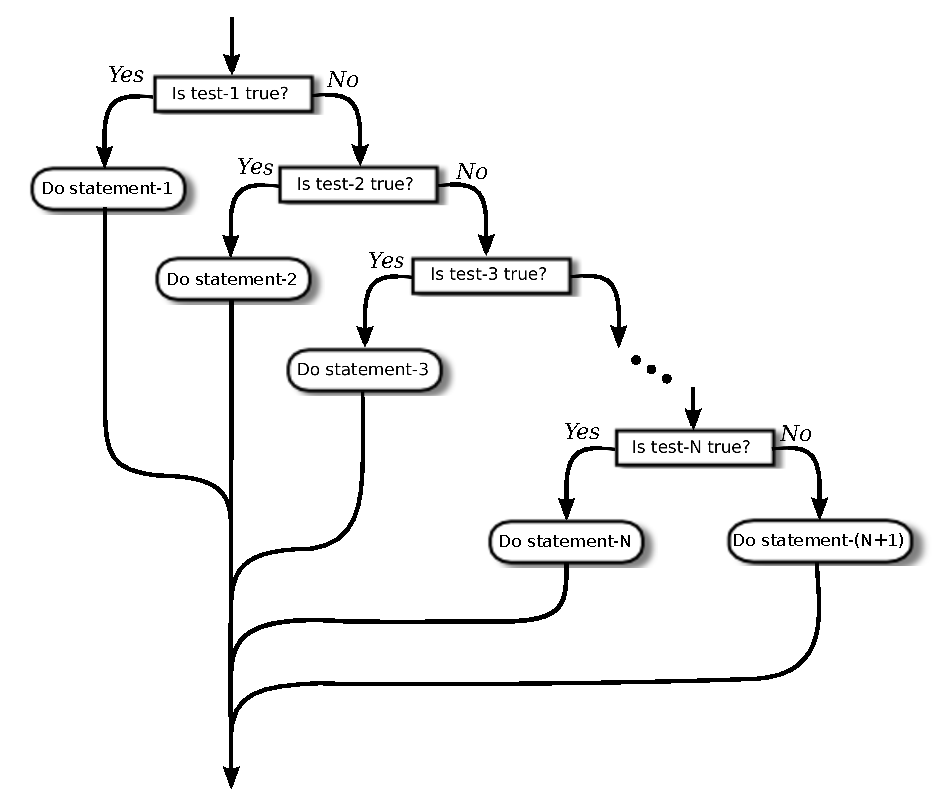
\includegraphics[scale=0.75]{images/multiway-if-flow-control.eps}
}




\subsection{If Statement Examples}\label{control.5.3}



As an example of using \code{if} statements, let's suppose that \code{x},
\code{y}, and \code{z} are variables of type \ptype{int}, and that each
variable has already been assigned a value. Consider the problem of printing
out the values of the three variables in increasing order. For example, if the
values are 42, 17, and 20, then the output should be in the order 17, 20,
42.


One way to approach this is to ask, where does \code{x} belong in the
list? It comes first if it's less than both \code{y} and \code{z}. It comes
last if it's greater than both \code{y} and \code{z}. Otherwise, it comes
in the middle. We can express this with a 3-way \code{if} statement, but we
still have to worry about the order in which \code{y} and \code{z} should
be printed. In pseudocode,

\displaycode{if (x \< y \&\& x \< z) \{
    output x, followed by y and z in their correct order
\}
else if (x \> y \&\& x \> z) \{
    output y and z in their correct order, followed by x
\}
else \{
    output x in between y and z in their correct order
\}}\donedisplaycode


\noindent Determining the relative order of \code{y} and \code{z} requires another
\code{if} statement, so this becomes

\displaycode{if (x \< y \&\& x \< z) \{        // x comes first
    if (y \< z)
       System.out.println( x + " " + y + " " + z );
    else
       System.out.println( x + " " + z + " " + y );
\}
else if (x \> y \&\& x \> z) \{   // x comes last
    if (y \< z)
       System.out.println( y + " " + z + " " + x );
    else
       System.out.println( z + " " + y + " " + x );
\}
else \{                       // x in the middle
    if (y \< z)
       System.out.println( y + " " + x + " " + z);
    else
       System.out.println( z + " " + x + " " + y);
\}}\donedisplaycode


\noindent You might check that this code will work correctly even if some of the
values are the same. If the values of two variables are the same, it doesn't
matter which order you print them in.


Note, by the way, that even though you can say in English ``if x is less than
y and z," you can't say in Java ``\code{if (x \< y \&\& z)}". The
\code{\&\&} operator can only be used between boolean values, so you
have to make separate tests, \code{x\<y} and \code{x\<z}, and then
combine the two tests with \code{\&\&}.


There is an alternative approach to this problem that begins by asking,
``which order should \code{x} and \code{y} be printed in?" Once that's
known, you only have to decide where to stick in \code{z}. This line of
thought leads to different Java code:

\displaycode{if ( x \< y ) \{  // x comes before y
   if ( z \< x )   // z comes first
      System.out.println( z + " " + x + " " + y);
   else if ( z \> y )   // z comes last
      System.out.println( x + " " + y + " " + z);
   else   // z is in the middle
      System.out.println( x + " " + z + " " + y);
\}
else \{          // y comes before x
   if ( z \< y )   // z comes first
      System.out.println( z + " " + y + " " + x);
   else if ( z \> x )  // z comes last
      System.out.println( y + " " + x + " " + z);
   else  // z is in the middle
      System.out.println( y + " " + z + " " + x);
\}}\donedisplaycode



Once again, we see how the same problem can be solved in many different
ways. The two approaches to this problem have not exhausted all the
possibilities. For example, you might start by testing whether \code{x} is
greater than \code{y}. If so, you could swap their values. Once you've done
that, you know that \code{x} should be printed before \code{y}.


\mybreak



Finally, let's write a complete program that uses an \code{if} statement
in an interesting way. I want a program that will convert measurements of
length from one unit of measurement to another, such as miles to yards or
inches to feet. So far, the problem is extremely under-specified. Let's say
that the program will only deal with measurements in inches, feet, yards, and
miles. It would be easy to extend it later to deal with other units. The user
will type in a measurement in one of these units, such as ``17 feet" or ``2.73
miles". The output will show the length in terms of \textbf{each} of
the four units of measure. (This is easier than asking the user which units to
use in the output.) An outline of the process is

\displaycode{Read the user's input measurement and units of measure
Express the measurement in inches, feet, yards, and miles
Display the four results}\donedisplaycode



The program can read both parts of the user's input from the same line by
using \code{TextIO.getDouble()} to read the numerical measurement and
\code{TextIO.getlnWord()} to read the unit of measure. The conversion into
different units of measure can be simplified by first converting the user's
input into inches. From there, the number of inches can easily be converted into feet, yards, and miles.
Before converting into inches, we have to test the input to determine which unit of measure the user has
specified:

\displaycode{Let measurement = TextIO.getDouble()
Let units = TextIO.getlnWord()
if the units are inches
   Let inches = measurement
else if the units are feet
   Let inches = measurement * 12         // 12 inches per foot
else if the units are yards
   Let inches = measurement * 36         // 36 inches per yard
else if the units are miles
   Let inches = measurement * 12 * 5280  // 5280 feet per mile
else
   The units are illegal!
   Print an error message and stop processing
Let feet = inches / 12.0
Let yards = inches / 36.0
Let miles = inches / (12.0 * 5280.0)
Display the results}\donedisplaycode



Since \code{units} is a \classname{String}, we can use
\code{units.equals("inches")} to check whether the specified unit of measure
is ``inches". However, it would be nice to allow the units to be specified as
``inch" or abbreviated to ``in". To allow these three possibilities, we can check
\code{if (units.equals("inches") || units.equals("inch") ||
units.equals("in"))}. It would also be nice to allow upper case letters, as
in ``Inches" or ``IN". We can do this by converting \code{units} to lower case
before testing it or by substituting the function
\code{units.equalsIgnoreCase} for \code{units.equals}.


In my final program, I decided to make things more interesting by allowing
the user to repeat the process of entering a measurement and seeing the
results of the conversion for each measurement.  The program will end only
when the user inputs 0. To program that, I just had to wrap the above algorithm
inside a \code{while} loop, and make sure that the loop ends when the user
inputs a~0. Here's the complete program:

\displaycode{/**
 * This program will convert measurements expressed in inches,
 * feet, yards, or miles into each of the possible units of
 * measure.  The measurement is input by the user, followed by
 * the unit of measure.  For example:  "17 feet", "1 inch", or
 * "2.73 mi".  Abbreviations in, ft, yd, and mi are accepted.
 * The program will continue to read and convert measurements
 * until the user enters an input of 0.
 */
 
 public class LengthConverter \{
 
    public static void main(String[] args) \{
       
       double measurement;  // Numerical measurement, input by user.
       String units;        // The unit of measure for the input, also
                            //    specified by the user.
       
       double inches, feet, yards, miles;  // Measurement expressed in
                                           //   each possible unit of
                                           //   measure.
       
       System.out.println("Enter measurements in inches, feet, yards, or miles.");
       System.out.println("For example:  1 inch    17 feet    2.73 miles");
       System.out.println("You can use abbreviations:   in   ft  yd   mi");
       System.out.println("I will convert your input into the other units");
       System.out.println("of measure.");
       System.out.println();
       
       while (true) \{
          
          /* Get the user's input, and convert units to lower case. */
          
          System.out.print("Enter your measurement, or 0 to end:  ");
          measurement = TextIO.getDouble();
          if (measurement == 0)
             break;  // Terminate the while loop.
          units = TextIO.getlnWord();            
          units = units.toLowerCase();  // convert units to lower case
          
          /* Convert the input measurement to inches. */
          
          if (units.equals("inch") || units.equals("inches") 
                                          || units.equals("in")) \{
              inches = measurement;
          \}
          else if (units.equals("foot") || units.equals("feet") 
                                          || units.equals("ft")) \{
              inches = measurement * 12;
          \}
          else if (units.equals("yard") || units.equals("yards") 
                                           || units.equals("yd")) \{
              inches = measurement * 36;
          \}
          else if (units.equals("mile") || units.equals("miles") 
                                             || units.equals("mi")) \{
              inches = measurement * 12 * 5280;
          \}
          else \{
              System.out.println("Sorry, but I don't understand \1"" 
                                                   + units + "\1".");
              continue;  // back to start of while loop
          \}
          
          /* Convert measurement in inches to feet, yards, and miles. */
          
          feet = inches / 12;
          yards = inches / 36;
          miles = inches / (12*5280);
          
          /* Output measurement in terms of each unit of measure. */
          
          System.out.println();
          System.out.println("That's equivalent to:");
          System.out.printf("\%12.5g", inches);
          System.out.println(" inches");
          System.out.printf("\%12.5g", feet);
          System.out.println(" feet");
          System.out.printf("\%12.5g", yards);
          System.out.println(" yards");
          System.out.printf("\%12.5g", miles);
          System.out.println(" miles");
          System.out.println();
       
       \} // end while
       
       System.out.println();
       System.out.println("OK!  Bye for now.");
       
    \} // end main()
    
 \} // end class LengthConverter
}\donedisplaycode


   

(Note that this program uses formatted output with the ``g" format specifier.  In this program,
we have no control over how large or how small the numbers might be.  It could easily make
sense for the user to enter very large or very small measurements.  The ``g" format will
print a real number in exponential form if it is very large or very small, and in the usual decimal form
otherwise.  Remember that in the format specification \code{\%12.5g}, the 5 is the total
number of significant digits that are to be printed, so we will always get the same number of
significant digits in the output, no matter what the size of the number.  If we had used an
``f" format specifier such as \code{\%12.5f}, the output would be in decimal form with
5 digits after the decimal point.  This would print the number 0.000000000745482 as \code{0.00000},
with no \textbf{significant} digits at all!
With the ``g" format specifier, the output would be \code{7.4549e-10}.)
   


\subsection{The Empty Statement}\label{control.5.4}



As a final note in this section, I will mention one more type of statement
in Java: the \newword{empty statement}. This is a statement
that consists simply of a semicolon and which tells the computer to
do nothing. The existence of the empty statement makes
the following legal, even though you would not ordinarily see a semicolon after
a~\}~:

\displaycode{if (x \< 0) \{
    x = -x;
\};}\donedisplaycode



The semicolon is legal after the \}, but the computer considers it to be an
empty statement, not part of the \code{if} statement. Occasionally, you might
find yourself using the empty statement when what you mean is, in fact, ``do
nothing." For example, the rather contrived \code{if} statement
   
\displaycode{if ( done )
   ;  // Empty statement
else
   System.out.println( "Not done yet.");}\donedisplaycode

   
\noindent does nothing when the \ptype{boolean} variable \code{done} is true,
and prints out ``Not done yet" when it is false. You can't just leave out the semicolon
in this example, since Java syntax requires an actual statement between the \code{if}
and the \code{else}.   I prefer, though, to use an empty block, consisting 
of~\{~and~\} with nothing between, for such cases.


Occasionally, stray empty statements can cause annoying, hard-to-find errors
in a program. For example, the following program segment prints out ``Hello"
just \textbf{once}, not ten times:

\displaycode{for (int i = 0; i \< 10; i++);
    System.out.println("Hello");}\donedisplaycode


\noindent Why? Because the ``;" at the end of the first line is a statement, and it is
this empty statement that is executed ten times. The \code{System.out.println}
statement is not really inside the \code{for} statement at all, so it is
executed just once, after the \code{for} loop has completed.  The
\code{for} loop just does nothing, ten times!



   



\section{The switch Statement}\label{control.6}

   

\start{{\Large T}he second branching statement} in Java is the
\code{switch} statement, which is introduced in this section. The
\code{switch} statement is used far less often than the \code{if} statement, but it
is sometimes useful for expressing a certain type of multiway branch.

   
\subsection{The Basic switch Statement}\label{control.6.1}



A switch statement allows you to test the value of an expression and,
depending on that value, to jump directly to some location within the switch statement.
Only expressions of certain types can be used.  The value of the expression
can be one of the primitive integer types \ptype{int},
\ptype{short}, or \ptype{byte}.
It can be the primitive \ptype{char} type.  
It can be \classname{String}.
Or it can be an enum type (see Subsection~\ref{basics.3.4} for an introduction to enums).  
In particular, note that the expression \textbf{cannot} be a \ptype{double} or 
\ptype{float} value.  


The positions within a switch statement to which it
can jump are marked with \newword{case labels} that take the form: 
``case~\bnf{constant}:".  The \bnf{constant} here is a literal of
the same type as the expression in the \code{switch}.
A case label marks the position the
computer jumps to when the expression evaluates to the given \bnf{constant} value. 
As the final case in a switch statement you can,
optionally, use the label ``default:", which provides a default jump point that
is used when the value of the expression is not listed in any case label.


A \code{switch} statement, as it is most often used, has the form:

\displaycode{switch (\bnf{expression}) \{
   case \bnf{constant-1}:
      \bnf{statements-1}
      break;
   case \bnf{constant-2}:
      \bnf{statements-2}
      break;
      .
      .   // (more cases)
      .
   case \bnf{constant-N}:
      \bnf{statements-N}
      break;
   default:  // optional default case
      \bnf{statements-(N+1)}
\} // end of switch statement}\donedisplaycode


\noindent This has exactly the same effect as the following multiway \code{if} statement,
but the \code{switch} statement can be more efficient because the computer
can evaluate one expression and jump directly to the correct case, 
whereas in the \code{if} statement, the
computer must evaluate up to \code{N} expressions before it knows which set of
statements to execute:

\displaycode{if (\bnf{expression} == \bnf{constant-1}) \{ // but use .equals for String!!
    \bnf{statements-2}
\} 
else if (\bnf{expression} == \bnf{constant-2}) \{ 
    \bnf{statements-3}
\} 
else
    .
    .
    .
else if (\bnf{expression} == \bnf{constant-N}) \{ 
    \bnf{statements-N}
\} 
else \{
    \bnf{statements-(N+1)}
\}}\donedisplaycode



The \code{break} statements in the \code{switch} are technically optional. The effect of a
\code{break} is to make the computer jump past the end of the switch statement,
skipping over all the remaining cases.
If you leave out the break statement, the computer will just forge ahead after
completing one case and will execute the statements associated with the next
case label. This is rarely what you want, but it is legal. (I will note here---although 
you won't understand it until you get to the next chapter---that
inside a subroutine, the \code{break} statement is sometimes replaced by a
\code{return} statement, which terminates the subroutine as well as the switch.)


Note that you can leave out one of the groups of statements entirely
(including the \code{break}). You then have two case labels in a row,
containing two different constants. This just means that the computer will jump
to the same place and perform the same action for each of the two
constants.


Here is an example of a switch statement. This is not a useful example, but
it should be easy for you to follow. Note, by the way, that the constants in
the case labels don't have to be in any particular order, but they must
all be different:

\displaycode{switch ( N ) \{   // (Assume N is an integer variable.)
   case 1:
      System.out.println("The number is 1.");
      break;
   case 2:
   case 4:
   case 8:
      System.out.println("The number is 2, 4, or 8.");
      System.out.println("(That's a power of 2!)");
      break;
   case 3:
   case 6:
   case 9:
      System.out.println("The number is 3, 6, or 9.");
      System.out.println("(That's a multiple of 3!)");
      break;
   case 5:
      System.out.println("The number is 5.");
      break;
   default:
      System.out.println("The number is 7 or is outside the range 1 to 9.");
\}}\donedisplaycode


   

The switch statement is pretty primitive as control structures go, and it's
easy to make mistakes when you use it. Java takes all its control structures
directly from the older programming languages C and C++. The switch statement
is certainly one place where the designers of Java should have introduced some
improvements.

   
   


\subsection{Menus and switch Statements}\label{control.6.2}



One application of \code{switch} statements is in processing menus. A menu
is a list of options. The user selects one of the options. The computer has to
respond to each possible choice in a different way. If the options are numbered
1, 2,~\dots, then the number of the chosen option can be used in a
\code{switch} statement to select the proper response.


In a \classname{TextIO}-based program, the menu can be presented as a numbered
list of options, and the user can choose an option by typing in its number.
Here is an example that could be used in a variation of the
\code{LengthConverter} example from the previous
section:

\displaycode{int optionNumber;   // Option number from menu, selected by user.
double measurement; // A numerical measurement, input by the user.
                    //    The unit of measurement depends on which
                    //    option the user has selected.
double inches;      // The same measurement, converted into inches.

/* Display menu and get user's selected option number. */

System.out.println("What unit of measurement does your input use?");
System.out.println();
System.out.println("         1.  inches");
System.out.println("         2.  feet");
System.out.println("         3.  yards");
System.out.println("         4.  miles");
System.out.println();
System.out.println("Enter the number of your choice: ");
optionNumber = TextIO.getlnInt();

/* Read user's measurement and convert to inches. */

switch ( optionNumber ) \{
   case 1:
       System.out.println("Enter the number of inches: ");
       measurement = TextIO.getlnDouble();
       inches = measurement;
       break;          
   case 2:
       System.out.println("Enter the number of feet: ");
       measurement = TextIO.getlnDouble();
       inches = measurement * 12;
       break;          
   case 3:
       System.out.println("Enter the number of yards: ");
       measurement = TextIO.getlnDouble();
       inches = measurement * 36;
       break;          
   case 4:
       System.out.println("Enter the number of miles: ");
       measurement = TextIO.getlnDouble();
       inches = measurement * 12 * 5280;
       break;
   default:
       System.out.println("Error!  Illegal option number!  I quit!");
       System.exit(1);          
\} // end switch

/* Now go on to convert inches to feet, yards, and miles... */}\donedisplaycode


\noindent This example could instead be written using a \classname{String}
in the \code{switch} statement:

\displaycode{String units;       // Unit of measurement, entered by user.
double measurement; // A numerical measurement, input by the user.
double inches;      // The same measurement, converted into inches.

/* Read the user's unit of measurement. */

System.out.println("What unit of measurement does your input use?");
System.out.print("Legal responses: inches, feet, yards, or miles : ");
units = TextIO.getln().toLowerCase();

/* Read user's measurement and convert to inches. */

System.out.print("Enter the number of " + units + ":  ");
measurement = TextIO.getlnDouble();

switch ( units ) \{
   case "inches":
       inches = measurement;
       break;          
   case "feet":
       inches = measurement * 12;
       break;          
   case "yards":
       inches = measurement * 36;
       break;          
   case "miles":
       inches = measurement * 12 * 5280;
       break;
   default:
       System.out.println("Wait a minute!  Illegal unit of measure!  I quit!");
       System.exit(1);          
\} // end switch}\donedisplaycode


   


\subsection{Enums in switch Statements}\label{control.6.3}

   

The type of the expression in a \code{switch} can be an enumerated
type.  In that case, the constants in the \code{case} labels must
be values from the enumerated type.  For example, suppose that the type of
the expression is the enumerated type \classname{Season}
defined by

\displaycode{enum Season \{ SPRING, SUMMER, FALL, WINTER \}}\donedisplaycode


\noindent and that the expression in a \code{switch} statement is an expression
of type \classname{Season}.  The constants in the case label must be chosen from among
the values \code{Season.SPRING}, \code{Season.SUMMER}, \code{Season.FALL}, or
\code{Season.WINTER}.  However, there is a quirk in the syntax:
when an enum  constant is used in a \code{case} label, only the simple name,
such as ``\code{SPRING}" is used, not the full name, such as ``\code{Season.SPRING}".
Of course, the computer already knows that the value in the \code{case} label
must belong to the enumerated type, since it can tell that from the type of expression
used, so there is really no need to specify the type name in the constant.  For example,
assuming that \code{currentSeason} is a variable of type \classname{Season},
then we could have the \code{switch} statement:
  
\displaycode{switch ( currentSeason ) \{
   case WINTER:    // ( NOT Season.WINTER ! )
      System.out.println("December, January, February");
      break;
   case SPRING:
      System.out.println("March, April, May");
      break;
   case SUMMER:
      System.out.println("June, July, August");
      break;
   case FALL:
      System.out.println("September, October, November");
      break;
\}}\donedisplaycode



\subsection{Definite Assignment and switch Statements}\label{control.6.4}

   

As a somewhat more realistic example, the following \code{switch} statement
makes a random choice among three possible alternatives.  Recall that the
value of the expression \code{(int)(3*Math.random())} is one of the
integers 0, 1, or 2, selected at random with equal probability, so the
\code{switch} statement below will assign one of the values
\code{"Rock"}, \code{"Paper"}, \code{"Scissors"} to \code{computerMove},
with probability 1/3 for each case:

\displaycode{switch ( (int)(3*Math.random()) ) \{
   case 0:
      computerMove = "Rock";
      break;
   case 1:
      computerMove = "Paper";
      break;
   case 2:
      computerMove = "Scissors";
      break;
\}}\donedisplaycode


\noindent Now, this \code{switch} statement is perfectly OK, but suppose that we use it in the
following code segment:
   
\displaycode{\newcode{String computerMove;}
switch ( (int)(3*Math.random()) ) \{
   case 0:
      computerMove = "Rock";
      break;
   case 1:
      computerMove = "Paper";
      break;
   case 2:
      computerMove = "Scissors";
      break;
\}
\newcode{System.out.println("The computer's move is " + computerMove);}  // ERROR!}\donedisplaycode


\noindent Now there is a subtle error on the last line!  The problem here is due to
definite assignment, the idea that the Java compiler must be able to determine
that a variable has definitely been assigned a value before its value is used.
Definite assignment was introduced in Subsection~\ref{control.1.4}.
In this example, it's true that the three cases in the \code{switch}
cover all the possibilities, but the compiler is not smart enough to figure
that out; it just sees that there is an integer-valued expression in the \code{switch}
but not all possible integer values are covered by the given cases.



A simple solution is to replace the final \code{case} in the \code{switch}
statement with \code{default}.  With a \code{default} case, all
possible values of the expression in the \code{switch} are certainly covered,
and the compiler knows that \code{computerMove} is definitely assigned
a value:

\displaycode{String computerMove;
switch ( (int)(3*Math.random()) ) \{
   case 0:
      computerMove = "Rock";
      break;
   case 1:
      computerMove = "Paper";
      break;
   \newcode{default}:
      computerMove = "Scissors";
      break;
\}
System.out.println("The computer's move is " + computerMove);  // OK!}\donedisplaycode




   

   



\section[Exceptions and try..catch]{Introduction to Exceptions and try..catch}\label{control.7}



\start{{\Large I}n addition to the control} structures that
determine the normal flow of control in a program, Java has a way to deal
with ``exceptional" cases that throw the flow of control off its normal
track.  When an error occurs during the execution of a program, the default
behavior is to terminate the program and to print an error message.  However,
Java makes it possible to ``catch" such errors and program a response different
from simply letting the program crash.  This is done with the
\newword{try..catch} statement.  In this section, we will
take a preliminary and incomplete look the \code{try..catch} statement,
leaving out a lot of the rather complex syntax of this statement.
Error handling is a complex topic, which we will return to in
Chapter~\ref{robustness}, and we will cover the full syntax
of \code{try..catch} at that time.
   
\subsection{Exceptions}\label{control.7.1}



The term \newword{exception} is used to refer to the type of
error that one might want to handle with a \code{try..catch}.  An
exception is an exception to the normal flow of control in the program.
The term is used in preference to ``error" because in some cases,
an exception might not be considered to be an error at all.  You can
sometimes think of an exception as just another way to organize
a program.
   

Exceptions in Java are represented as objects of type \classname{Exception}.
Actual exceptions are usually defined by subclasses of \classname{Exception}.
Different subclasses represent different types of exceptions.  We will look at only
two types of exception in this section:  \classname{NumberFormatException}
and \classname{IllegalArgumentException}.
   

A \classname{NumberFormatException} can occur when an attempt
is made to convert a string into a number.  Such conversions are done by
the functions \code{Integer.parseInt} and \code{Double.parseDouble}.
(See Subsection~\ref{basics.5.7}.)  Consider the function call \code{Integer.parseInt(str)}
where \code{str} is a variable of type \classname{String}.
If the value of \code{str} is the string \code{"42"}, then the
function call will correctly convert the string into the \ptype{int}~42.
However, if the value of \code{str} is, say, \code{"fred"}, the function call 
will fail because \code{"fred"} is not a legal string representation of
an \ptype{int} value.  In this case, an exception of type
\classname{NumberFormatException} occurs.  If nothing is done
to handle the exception, the program will crash.


An \classname{IllegalArgumentException} can occur when an illegal
value is passed as a parameter to a subroutine.  For example, if a subroutine
requires that a parameter be greater than or equal to zero, an \classname{IllegalArgumentException}
might occur when a negative value is passed to the subroutine.
How to respond to the illegal value is up to the person who wrote the subroutine, 
so we can't simply say that every illegal parameter value will result in an
\classname{IllegalArgumentException}.  However, it is a common response.



\subsection{try..catch}\label{control.7.2}

   

When an exception occurs, we say that the exception is ``thrown".
For example, we say that \code{Integer.parseInt(str)} \newword{throws}
an exception of type \classname{NumberFormatException} when the value of 
\code{str} is illegal.  When an exception is thrown, it is possible
to ``catch" the exception and prevent it from crashing the program.  This is
done with a \newword{try..catch} statement.  In simplified
form, the syntax for a \code{try..catch} can be:

\displaycode{try \{
   \bnf{statements-1}
\}
catch ( \bnf{exception-class-name}  \bnf{variable-name} ) \{
   \bnf{statements-2}
\}}\donedisplaycode

   
\noindent The \bnf{exception-class-name} could be \classname{NumberFormatException},
\classname{IllegalArgumentException}, or some other exception class.
When the computer executes this \code{try..catch} statement, 
it executes the statements in the \code{try}
part.  If no exception occurs during the execution of \bnf{statements-1}, then the computer
just skips over the \code{catch} part and proceeds with the rest of the program.
However, if an exception of type \bnf{exception-class-name} occurs during the
execution of \bnf{statements-1}, the computer immediately jumps from the point where the
exception occurs to the
\code{catch} part and executes \bnf{statements-2}, skipping any remaining statements in
\bnf{statements-1}.  
Note that only one type of exception is caught; if some other type of exception occurs
during the execution of \bnf{statements-1}, it will crash the program as usual.


During the execution of \bnf{statements-2}, the
\bnf{variable-name} represents the exception object, so that you can, for example,
print it out.  The exception object contains information about the cause of the exception.
This includes an error message, which will be displayed if you print out the exception object.


After the end of the
\code{catch} part, the computer proceeds with the rest of the program;
the exception has been caught and handled and does not crash the program.

   

By the way, note that the braces, \{ and \}, are part of the syntax of the
\code{try..catch} statement.  They are required even if there is only one
statement between the braces.  This is different from the other statements we
have seen, where the braces around a single statement are optional.
   

As an example, suppose that \code{str} is a variable of type \classname{String}
whose value might or might not represent a legal real number.  Then we could say:
   
\displaycode{double x;
try \{
   x = Double.parseDouble(str);
   System.out.println( "The number is " + x );
\}
catch ( NumberFormatException e ) \{
   System.out.println( "Not a legal number." );
   x = Double.NaN;
\}}\donedisplaycode

   
\noindent If an error is thrown by the call to \code{Double.parseDouble(str)}, then the
output statement in the \code{try} part is skipped, and the statement in the
\code{catch} part is executed.  (In this example, I set \code{x} to be
the value \code{Double.NaN} when an exception occurs.  \code{Double.NaN}
is the special ``not-a-number" value for type \ptype{double}.)

   

It's \textbf{not} always a good idea to catch exceptions and continue with the program.  Often
that can just lead to an even bigger mess later on, and it might be better just to let
the exception crash the program at the point where it occurs.  However, sometimes it's
possible to recover from an error.


Suppose, for example, we want a program that will
find the average of a sequence of real numbers entered by the user, and we want the user
to signal the end of the sequence by entering a blank line.  (This is similar
to the sample program \sourceref{ComputeAverage.java} from Section~\ref{control.3},
but in that program the user entered a zero to signal end-of-input.)
If we use \code{TextIO.getlnInt()}
to read the user's input, we will have no way of detecting the blank line, since that
function simply skips over blank lines.  A solution is to use \code{TextIO.getln()}
to read the user's input.  This allows us to detect a blank input line, and we can
convert non-blank inputs to numbers using \code{Double.parseDouble}.  And we
can use \code{try..catch} to avoid crashing the program when the user's input
is not a legal number.  Here's the program:

\displaycode{public class ComputeAverage2 \{

   public static void main(String[] args) \{
       String str;     // The user's input.
       double number;  // The input converted into a number.
       double total;   // The total of all numbers entered.
       double avg;     // The average of the numbers.
       int count;      // The number of numbers entered.
       total = 0;
       count = 0;
       System.out.println("Enter your numbers, press return to end.");
       while (true) \{
          System.out.print("? ");
          str = TextIO.getln();
          if (str.equals("")) \{
             break; // Exit the loop, since the input line was blank.
          \}
          try \{
              number = Double.parseDouble(str);
              // If an error occurs, the next 2 lines are skipped!
              total = total + number;
              count = count + 1;
          \}
          catch (NumberFormatException e) \{
              System.out.println("Not a legal number!  Try again.");
          \}
       \}
       avg = total/count;
       System.out.printf("The average of \%d numbers is \%1.6g\%n", count, avg);
   \}

\}}\donedisplaycode



   
\subsection{Exceptions in TextIO}\label{control.7.3}

   

When \code{TextIO} reads a numeric value from the user, it makes sure
that the user's response is legal, using a technique similar to the \code{while}
loop and \code{try..catch} in the previous example.  However, \code{TextIO}
can read data from other sources besides the user.  (See Subsection~\ref{basics.4.4}.)
When it is reading from a file,
there is no reasonable way for \code{TextIO} to recover from an illegal
value in the input, so it responds by throwing an exception.
To keep things simple, \code{TextIO} only throws exceptions of type
\classname{IllegalArgumentException}, no matter what type of error it
encounters.  For example, an exception
will occur if an attempt is made to read from a file after all the data in the
file has already been read.  In \code{TextIO}, the exception is of type
\classname{IllegalArgumentException}.
If you have a better response to file errors than to let the
program crash, you can use a \code{try..catch} to catch exceptions of
type \classname{IllegalArgumentException}.  

   

As an example, we will look at yet another number-averaging program.  In this case,
we will read the numbers from a file.
Assume that the file contains nothing but real numbers, and we
want a program that will read the numbers and find their sum and their average.
Since it is unknown how many numbers are in the
file, there is the question of when to stop reading.  One approach is simply
to try to keep reading indefinitely.  When the end of the file is reached,
an exception occurs.  This exception is not really an error---it's just
a way of detecting the end of the data, so we can catch the exception and
finish up the program.  We can read the data in a \code{while~(true)} loop
and break out of the loop when an exception occurs.  This is an example
of the somewhat unusual technique of using an exception as part of the 
expected flow of control in a program.

   

To read from the file, we need to know the file's name.  To make the program
more general, we can let the user enter the file name, instead of hard-coding
a fixed file name in the program.  However, it is possible that the user will
enter the name of a file that does not exist.  When we use \code{TextIO.readfile}
to open a file that does not exist, an exception of type 
\classname{IllegalArgumentException} occurs.  We can catch
this exception and ask the user to enter a different file name.  Here is
a complete program that uses all these ideas:

\displaycode{/**
 * This program reads numbers from a file.  It computes the sum and 
 * the average of the numbers that it reads.  The file should contain 
 * nothing but numbers of type double; if this is not the case, the 
 * output will be the sum and average of however many numbers were 
 * successfully read from the file.  The name of the file will be
 * input by the user.
 */
public class AverageNumbersFromFile \{
   
   public static void main(String[] args) \{
            
      while (true) \{
         String fileName;  // The name of the file, to be input by the user.
         System.out.print("Enter the name of the file: ");
         fileName = TextIO.getln();
         try \{
            TextIO.readFile( fileName );  // Try to open the file for input.
            break;  // If that succeeds, break out of the loop.
         \}
         catch ( IllegalArgumentException e ) \{
            System.out.println("Can't read from the file \1"" + fileName + "\1".");
            System.out.println("Please try again.\1n");
         \}
      \}
      
      /* At this point, TextIO is reading from the file. */
      
      double number;  // A number read from the data file.
      double sum;     // The sum of all the numbers read so far.
      int count;      // The number of numbers that were read.
      
      sum = 0;
      count = 0;
      
      try \{
         while (true) \{ // Loop ends when an exception occurs.
             number = TextIO.getDouble();
             count++;  // This is skipped when the exception occurs
             sum += number;
         \}
      \}
      catch ( IllegalArgumentException e ) \{
         // We expect this to occur when the end-of-file is encountered.
         // We don't consider this to be an error, so there is nothing to do
         // in this catch clause.  Just proceed with the rest of the program.
      \}
      
      // At this point, we've read the entire file.
      
      System.out.println();
      System.out.println("Number of data values read: " + count);
      System.out.println("The sum of the data values: " + sum);
      if ( count == 0 )
         System.out.println("Can't compute an average of 0 values.");
      else
         System.out.println("The average of the values:  " + (sum/count));
      
   \}

\}}\donedisplaycode
  


   

   



\section{Introduction to Arrays}\label{control.7a}



\start{{\Large I}n previous sections of this chapter,} we have 
already covered all of Java's control structures.  But before moving on to the next chapter, we will
take preliminary looks at two addition topics that are at least somewhat related to control structures.

This section
is an introduction to arrays.  Arrays are a basic and very commonly used
data structure, and array processing is often an exercise in using control
structures. The next section will
introduce computer graphics and will allow you to apply what you know
about control structures in another context.


\subsection{Creating and Using Arrays}\label{control.7a.1}



A \newword{data structure} consists of a number of data items
chunked together so that they can be treated as a unit.  An \newword{array} is
a data structure in which the items are arranged as a numbered sequence,
so that each individual item can be referred to by its position number.
In Java---but not in other programming languages---all the items must 
be of the same type, and the numbering always starts at zero.
You will need to learn several new terms to talk about arrays:
The number of items in an array is called the
\newword{length} of the array. 
The type of the individual items in an array is called the 
\newword{base type} of the array. And the position number of an
item in an array is called the \newword{index} of that item.


Suppose that you want to write a program that will process the names of, say, one thousand people.
You will need a way to deal with all that data.  Before you knew about arrays,
you might have thought that the program would need a thousand variables to hold
the thousand names, and if you wanted to print out all the names, you would need
a thousand print statements.  Clearly, that would be ridiculous!  In reality,
you can put all the names into an array.  The array is a represented by a single
variable, but it holds the entire list of names.  The length of the array would
be 1000, since there are 1000 individual names.  The base type of the array
would be \classname{String} since the items in the array are
strings.  The first name would be at index 0 in the array, the second name
at index 1, and so on, up to the thousandth name at index 999.


The base type of an array can be any Java type, but for now, we will stick to
arrays whose base type is \classname{String} or one of the eight primitive
types.   If the base type of an
array is \ptype{int}, it is referred to as an ``array of \ptype{ints}." An
array with base type \classname{String} is referred to as an ``array of
\classname{Strings}." However, an array is not, properly speaking, a list of
integers or strings or other \textbf{values}. It is better thought of
as a list of \textbf{variables} of type \ptype{int}, or a list of variables of type
\classname{String}, or of some other type. As always, there is some potential for
confusion between the two uses of a variable: as a name for a memory location
and as a name for the value stored in that memory location. Each position in an
array acts as a variable. Each position can hold a value of a specified type
(the base type of the array), just as a variable can hold a value.
The value can be changed at any time, just as the value of a variable can be
changed.  The items in an array---really, the individual variables that make up the
array---are more often referred to as the \newword{elements} 
of the array.


As I mentioned above, when you use an array in a program, you can use a variable
to refer to array as a whole.  But you often need to refer to the individual elements
of the array.  The name for an element of an array is based on the name for the array
and the index number of the element.  The syntax for referring to an element
looks, for example, like this:  \code{namelist[7]}.  Here, \code{namelist}
is the variable that names the array as a whole, and \code{namelist[7]} refers to the
element at index 7 in that array.   That is, to refer to an element of an array,
you use the array name, followed by element index enclosed in square brackets.
An element name of this form can be used like any other variable: You can assign
a value to it, print it out, use it in an expression.


An array also contains a kind of variable representing its length.  For example,
you can refer to the length of the array \code{namelist} as \code{namelist.length}.
However, you cannot assign a value to \code{namelist.length}, since the length of an
array cannot be changed.



Before you can use a variable to refer to an array, that
variable must be declared, and it must
have a type.  For an array of \classname{Strings}, for example,
the type for the array variable would be \atype{String\hbox{[\hskip2pt]}}, and
for an array of \ptype{ints}, it would be \atype{int\hbox{[\hskip2pt]}}.
In general, an array type consists of the base type of the array followed
by a pair of empty square brackets.  Array types can be used to declare
variables; for example,

\displaycode{String[] namelist;
int[] A;
double[] prices;
}\donedisplaycode


\noindent and variables declared in this way can refer to arrays.  However, declaring
a variable does not make the actual array.  Like all variables, an array variable has
to be assigned a value before it can be used.  In this case, the value is
an array.  Arrays have to be created using a special syntax.  (The syntax
is related to the fact that arrays in Java are actually objects, but that doesn't
need to concern us here.)  Arrays are created with an operator named \newword{new}.
Here are some examples:

\displaycode{namelist = new String[1000];
A = new int[5];
prices = new double[100];}\donedisplaycode


\noindent The general syntax is

\displaycode{\bnf{array-variable} = new \bnf{base-type}[\bnf{array-length}];}\donedisplaycode


\noindent The length of the array can be given as either an integer or an integer-valued
expression.  For example, after the assignment statement
``\code{A~=~new~int[5];}", \code{A} is an array
containing the five integer elements \code{A[0]}, \code{A[1]}, \code{A[2]}, 
\code{A[3]}, and \code{A[4]}.  Also, \code{A.length} would have
the value~5.  It's useful to have a picture in mind:


\par\dumpfigure{
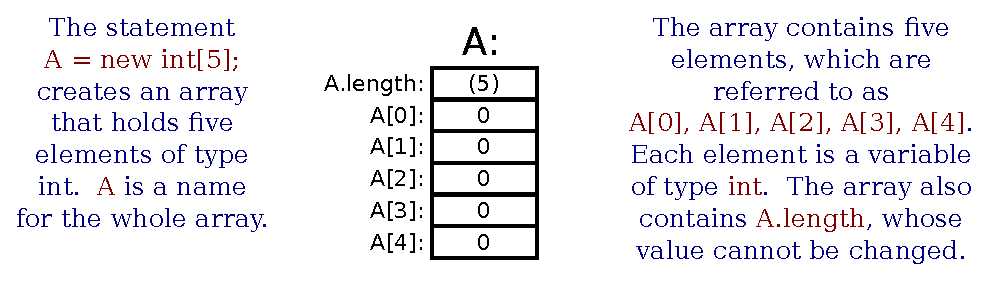
\includegraphics[scale=0.75]{images/array-of-ints.eps}
}

   

When you create an array of \ptype{int}, each element of the array is
automatically initialized to zero.  Any array of numbers is filled with zeros
when it is created.  An array of \ptype{boolean} is filled with the
value \code{false}.  And an array of \ptype{char} is filled
with the character that has Unicode code number zero.  (For an array of
\classname{String}, the initial value is \code{null},
a special value used for objects that we won't encounter officially until
Section~\ref{OOP.1}.)




\subsection{Arrays and For Loops}\label{control.7a.2}



A lot of the real power of arrays comes from the fact that
the index of an element can be given by an integer variable or
even an integer-valued expression.  For example, if \code{list}
is an array and \code{i} is a variable of type \ptype{int},
then you can use \code{list[i]} and even \code{list[2*i+1]}
as variable names.  The meaning of \code{list[i]} depends on
the value of \code{i}.  This becomes especially useful when we want to
process all the elements of an array, since that can be
done with a \code{for} loop.  For example, to print out
all the items in an array, \code{list}, we can just
write

\displaycode{
int i;  // the array index
for (i = 0; i \< list.length; i++) \{
    System.out.println( list[i] );
\}}\donedisplaycode


\noindent The first time through the loop, \code{i} is 0, and \code{list[i]}
refers to \code{list[0]}. So, it is the value stored in the variable
\code{list[0]} that is printed. The second time through the loop, \code{i}
is 1, and the value stored in \code{list[1]} is printed. The loop ends after
printing the value of \code{list[4]}, when \code{i} becomes equal to 5 and
the continuation condition ``\code{i~\<~list.length}" is no longer true. This
is a typical example of using a loop to process an array.


Let's look at a few more examples.  Suppose that \code{A} is an array
of \ptype{double}, and we want to find the average of all the elements of
the array.  We can use a \code{for} loop to add up the numbers, and then
divide by the length of the array to get the average:

\displaycode{double total;    // The sum of the numbers in the array.
double average;  // The average of the numbers.
int i;  // The array index.
total = 0;
for ( i = 0; i \< A.length; i++ ) \{
    total = total + A[i];  // Add element number i to the total.
\}
average = total / A.length;  // A.length is the number of items}\donedisplaycode



Another typical problem is to find the largest number in the array \code{A}. The
strategy is to go through the array, keeping track of the largest number found
so far. We'll store the largest number found so far in a variable called
\code{max}. As we look through the array, whenever we find a number larger
than the current value of \code{max}, we change the value of \code{max} to
that larger value. After the whole array has been processed, \code{max} is
the largest item in the array overall. The only question is, what should the
original value of \code{max} be? One possibility is to start with
\code{max} equal to \code{A[0]}, and then to look through the rest of the
array, starting from \code{A[1]}, for larger items:

\displaycode{double max;  // The largest number seen so far.
max = A[0];   // At first, the largest number seen is A[0].
int i;
for ( i = 1; i \< A.length; i++ ) \{
    if (A[i] \> max) \{
       max = A[i];
    \}
\}
// at this point, max is the largest item in A}\donedisplaycode



Sometimes, you only want to process some elements of the array.  In that
case, you can use an \code{if} statement inside the \code{for}
loop to decide whether or not to process a given element.  Let's look
at the problem of averaging the elements of an array, but this time,
suppose that we only want to average the non-zero elements.  In this case,
the number of items that we add up can be less than the length of the array,
so we will need to keep a count of the number of items added to the sum:

\displaycode{double total;    // The sum of the non-zero numbers in the array.
int count;       // The number of non-zero numbers.
double average;  // The average of the non-zero numbers.
int i;
total = 0;
count = 0;
for ( i = 0; i \< A.length; i++ ) \{
    if ( A[i] != 0 ) \{
        total = total + A[i];  // Add element to the total
        count = count + 1;     //      and count it.
    \}
\}
if (count == 0) \{
    System.out.println("There were no non-zero elements.");
\}
else \{
    average = total / count;  // Divide by number of items
    System.out.printf("Average of \%d elements is \%1.5g\%n",
                            count, average);
\}}\donedisplaycode






\subsection{Random Access}\label{control.7a.3}



So far, my examples of array processing have used \newword{sequential access}. 
That is, the elements of the array were
processed one after the other in the sequence in which they occur in the array.
But one of the big advantages of arrays is that they allow \newword{random access}. 
That is, every element of the array is equally accessible at any given time.


As an example, let's look at a well-known problem called the birthday
problem: Suppose that there are \code{N} people in a room. What's the chance
that there are two people in the room who have the same birthday? (That is,
they were born on the same day in the same month, but not necessarily in the
same year.) Most people severely underestimate the probability. We will actually
look at a different version of the question:  Suppose you choose people at random
and check their birthdays. How many people will you check before you find one
who has the same birthday as someone you've already checked? Of course, the
answer in a particular case depends on random factors, but we can simulate the
experiment with a computer program and run the program several times to get an
idea of how many people need to be checked on average.


To simulate the experiment, we need to keep track of each birthday that we
find. There are 365 different possible birthdays. (We'll ignore leap years.)
For each possible birthday, we need to keep track of whether or not we
have already found a person who has that birthday.
The answer to this question is a boolean value, true or false. To hold the data
for all 365 possible birthdays, we can
use an array of 365 boolean values:

\displaycode{boolean[] used; 
used = new boolean[365];}\donedisplaycode



For this problem, the days of the year are numbered from 0 to 364. The value of
\code{used[i]} is true if someone has been selected whose birthday is day
number \code{i}. Initially, all the values in the array are
false. (Remember that this is done automatically when the array is created.)
When we select someone whose birthday is day number \code{i}, we first
check whether \code{used[i]} is \code{true}. If it is \code{true}, then this is the second person
with that birthday. We are done. On the other hand, if \code{used[i]} is \code{false}, we set
\code{used[i]} to be \code{true} to record the fact that we've encountered someone
with that birthday, and we go on to the next person. Here is a program that
carries out the simulated experiment (of course, in the program, there are
no simulated people, only simulated birthdays):

\displaycode{/**
 * Simulate choosing people at random and checking the day of the year they 
 * were born on.  If the birthday is the same as one that was seen previously, 
 * stop, and output the number of people who were checked.
 */
public class BirthdayProblem \{

   public static void main(String[] args) \{

       boolean[] used;  // For recording the possible birthdays
                        //   that have been seen so far.  A value
                        //   of true in used[i] means that a person
                        //   whose birthday is the i-th day of the
                        //   year has been found.

       int count;       // The number of people who have been checked.

       used = new boolean[365];  // Initially, all entries are false.
   
       count = 0;

       while (true) \{
             // Select a birthday at random, from 0 to 364.
             // If the birthday has already been used, quit.
             // Otherwise, record the birthday as used.

          int birthday;  // The selected birthday.
          birthday = (int)(Math.random()*365);
          count++;

          System.out.printf("Person \%d has birthday number \%d", count, birthday);
          System.out.println();

          if ( used[birthday] ) \{  
                // This day was found before; it's a duplicate.  We are done.
             break;
          \}

          used[birthday] = true;

       \} // end while

       System.out.println();
       System.out.println("A duplicate birthday was found after " 
                                             + count + " tries.");
   \}

\} // end class BirthdayProblem}\donedisplaycode



\noindent You should study the program to understand how it works and how
it uses the array.  Also,
try it out!  You will probably find that a duplicate
birthday tends to occur sooner than you expect.





\subsection{Partially Full Arrays}\label{control.7a.4}



Consider an application where the number of items that we want to store in
an array changes as the program runs. Since the size of the array can't
be changed, a separate counter variable must be used to keep track of
how many spaces in the array are in use. (Of course, every space in the array
has to contain something; the question is, how many spaces contain useful or
valid items?)


Consider, for example, a program that reads positive integers entered by the
user and stores them for later processing. The program stops reading when the
user inputs a number that is less than or equal to zero. The input numbers can
be kept in an array, \code{numbers}, of type \atype{int\hbox{[\hskip2pt]}}. Let's say that
no more than 100 numbers will be input. Then the size of the array can be fixed
at 100. But the program must keep track of how many numbers have actually been
read and stored in the array. For this, it can use an integer variable.
Each time a number is stored in the array, we have to count it;
that is, value of the counter variable must be incremented by one. 
One question is, when we add a new item to the array, where do we put
it?  Well, if the number of items is \code{count}, then they would
be stored in the array in positions number 0, 1, \dots, (count-1).
The next open spot would be position number \code{count}, so that's
where we should put the new item.


As a rather silly example, let's write a program that
will read the numbers input by the user and then print them in the reverse of the
order in which they were entered.  Assume that an input value equal to zero
marks the end of the data.
(This is, at least, a processing task that requires that the numbers be saved
in an array. Note that many types of processing, such as finding the sum or
average or maximum of the numbers, can be done without saving the individual
numbers.)

\displaycode{public class ReverseInputNumbers \{

   public static void main(String[] args) \{
   
     int[] numbers;  // An array for storing the input values.
     int count;      // The number of numbers saved in the array.
     int num;        // One of the numbers input by the user.
     
     numbers = new int[100];   // Space for 100 ints.
     count = 0;                // No numbers have been saved yet.
     
     System.out.println("Enter up to 100 positive integers; enter 0 to end.");
     
     while (true) \{   // Get the numbers and put them in the array.
        System.out.print("? ");
        num = TextIO.getlnInt();
        if (num \<= 0) \{
              // Zero marks the end of input; we have all the numbers.
           break;
        \}
        numbers[count] = num;  // Put num in position count.
        count++;  // Count the number
     \}
     
     System.out.println("\1nYour numbers in reverse order are:\1n");
     
     for (int i = count - 1; i \>= 0; i--) \{
         System.out.println( numbers[i] );
     \}
     
   \} // end main();
   
\}  // end class ReverseInputNumbers}\donedisplaycode



It is especially important to note how the variable \code{count} plays a
dual role. It is the number of items that have been entered into the array.
But it is also the index of the next available spot in the array.


 When the time comes to print
out the numbers in the array, the last occupied spot in the array is location
\code{count~-~1}, so the \code{for} loop prints out values starting from
location \code{count~-~1} and going down to 0.  This is also a nice
example of processing the elements of an array in reverse order.


\mybreak



You might wonder what would happen in this program if the user tries to input
more than 100 numbers.  The result would be an error that would crash the
program.  When the user enters the 101-st number, the program tries to store
that number in an array element \code{number[100]}.  However, there is
no such array element.  There are only 100 items in the array, and the index
of the last item is 99.  The attempt to use \code{number[100]}
generates an exception of type \classname{ArrayIndexOutOfBoundsException}.
Exceptions of this type are a common source of run-time errors in programs that use arrays.




\subsection{Two-dimensional Arrays}\label{control.7a.5}



The arrays that we have considered so far are ``one-dimensional."  This means that the
array consists of a sequence of elements that can be thought of as being laid out along a line.
It is also possible to have \newword{two-dimensional arrays}, where the elements can
be laid out in a rectangular grid.  We consider them only briefly here, but will return
to the topic in Section~\ref{arrays.5}.


In a two-dimensional, or ``2D," array, the elements can be
arranged in rows and columns.  Here, for example, is a 2D array of \ptype{int}
that has five rows and seven columns:


\par\dumpfigure{
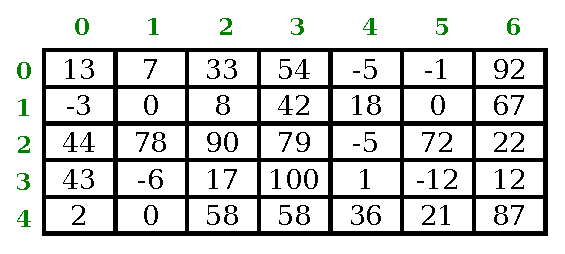
\includegraphics[scale=0.75]{images/two-d-array.eps}
}


\noindent This 5-by-7 grid contains a total of 35 elements.
The rows in a 2D array are numbered 0, 1, 2, \dots, up to the number of rows minus one.
Similarly, the columns are numbered from zero up to the number of columns minus one.  Each individual
element in the array can be picked out by specifying its row number and its column number.
(The illustration shown here is not what the array actually looks like in the computer's
memory, but it does show the logical structure of the array.)


In Java, the syntax for two-dimensional arrays is similar to the syntax for one-dimensional
arrays, except that an extra index is involved, since picking out an element requires both
a row number and a column number.  For example, if \code{A} is a 2D array of \ptype{int}, then
\code{A[3][2]} would be the element in row~3, column~2.  That would pick out the
number 17 in the array shown above.  The type for \code{A}
would be given as \atype{int\hbox{[\hskip2pt]}\hbox{[\hskip2pt]}}, with two pairs of empty brackets.  To declare the
array variable and create the array, you could say,

\displaycode{int[][]  A;
A  =  new int[5][7];}\donedisplaycode


\noindent The second line creates a 2D array with 5 rows and 7 columns.  Two-dimensional arrays
are often processed using nested \code{for} loops.  For example, the following code 
segment will print out the elements of \code{A} in neat columns:

\displaycode{int row, col;  // loop-control-variables for accessing rows and columns in A
for ( row = 0; row \< 5; row++ ) \{
    for ( col = 0; col \< 7; col++ ) \{
        System.out.printf( "\%7d",  A[row][col] );
    \}
    System.out.println();
\}}\donedisplaycode



\noindent The base type of a 2D array can be anything, so you can have arrays of type
\atype{double\hbox{[\hskip2pt]}\hbox{[\hskip2pt]}}, \atype{String\hbox{[\hskip2pt]}\hbox{[\hskip2pt]}}, and so on.


There are some natural uses for 2D arrays.  For example,
a 2D array can be used to store the contents of the board in a game such as
chess or checkers.  And an example in Subsection~\ref{subroutines.6.3} uses a 2D array
to hold the colors of a grid of colored squares.  But sometimes 
two-dimensional arrays are used in problems in which the grid is
not so visually obvious. Consider a company that owns 25 stores. Suppose that
the company has data about the profit earned at each store for each month in
the year 2014. If the stores are numbered from 0 to 24, and if the twelve
months from January 2014 through December 2014 are numbered from 0 to 11, then
the profit data could be stored in an array, \code{profit}, created as
follows:

\displaycode{double[][]  profit;
profit  =  new double[25][12];}\donedisplaycode


\noindent \code{profit[3][2]} would be the amount of profit earned at store number 3
in March, and more generally, \code{profit[storeNum][monthNum]} would be the
amount of profit earned in store number \code{storeNum} in month number
\code{monthNum} (where the numbering, remember, starts from zero).


Let's assume that the \code{profit} array has already been filled with
data. This data can be processed in a lot of interesting ways. For example, the
total profit for the company---for the whole year from all its stores---can
be calculated by adding up all the entries in the array:

\displaycode{double totalProfit;  // Company's total profit in 2014.
int store, month;  // variables for looping through the stores and the months
totalProfit = 0;
for ( store = 0; store \< 25; store++ ) \{
   for ( month = 0; month \< 12; month++ )
      totalProfit += profit[store][month];
\}}\donedisplaycode



Sometimes it is necessary to process a single row or a single column of an
array, not the entire array. For example, to compute the total profit earned by
the company in December, that is, in month number 11, you could use the
loop:

\displaycode{double decemberProfit;
int storeNum;
doubleProfit = 0.0;
for ( storeNum = 0; storeNum \< 25; storeNum++ ) \{
   decemberProfit += profit[storeNum][11];
\}}\donedisplaycode



Two-dimensional arrays are sometimes useful, but they are much less common
than one-dimensional arrays.  Java actually allows arrays of even higher dimension,
but they are only rarely encountered in practice.






   



\section[GUI Programming]{Introduction to GUI Programming}\label{control.8}



\start{{\Large F}or the past two chapters}, you've been learning the
sort of programming that is done inside a single subroutine, ``programming in the small."
In the rest of this
book, we'll be more concerned with the larger scale structure of programs, but
the material that you've already learned will be an important foundation for
everything to come.  In this section, we see how techniques that you have  
learned so far can be applied in the context of graphical programming.


When you run a GUI program, it opens one or more windows on your computer
screen.  As a programmer, you can have complete control over what appears in the
window and how the user can interact with it.  For our first encounter, we look
at one simple example: the ability of a program to display simple shapes like
rectangles and lines in the window, with no user interaction.  For now, the
main point is to take a look at how programming-in-the-small can be used in other contexts besides
text-based, command-line-style programs.   You will see that
a knowledge of programming-in-the-small applies to writing the guts of
any subroutine, not just \code{main()}.

\subsection{Drawing Shapes}\label{control.8.1}



To understand computer graphics, you need to know a little about pixels and 
coordinate systems.  The computer screen is made up of small squares called 
\newword{pixels}, arranged in rows and columns, usually about 100 pixels
per inch.  The computer controls the color of the pixels, and drawing is done by
changing the colors of individual pixels.  Each pixel has a pair of integer coordinates,
often called \textit{x} and \textit{y}, that specify the pixel's horizontal and vertical
position.  For a graphics context drawing to a rectangular area on the screen,
the coordinates of the pixel in the upper left corner of the rectangle are (0,0).
The \textit{x} coordinate increases from the left to right, and the \textit{y}
coordinate increases from top to bottom.  Shapes are specified using pixels.
For example, a rectangle is specified by the \textit{x} and \textit{y} coordinates of
its upper left corner and by its width and height measured in pixels.
Here's a picture of a rectangular drawing area, showing the ranges of \textit{x}
and \textit{y} coordinates.  The ``width" and ``height" in this picture are
give the size of the drawing area, in pixels:



\par\dumpfigure{
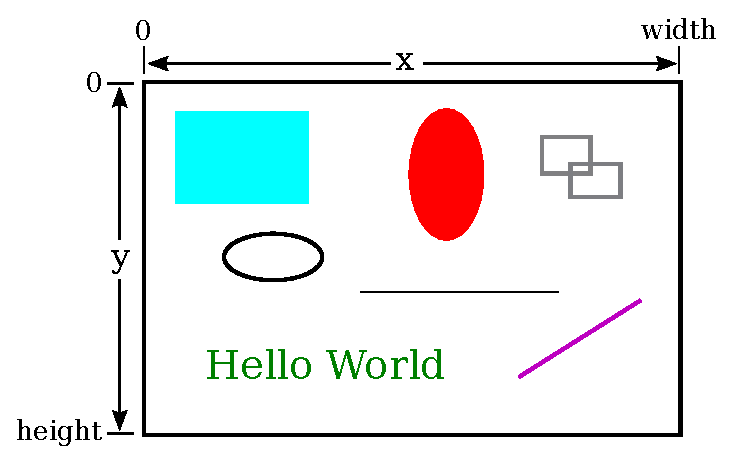
\includegraphics[scale=0.6]{images/coords-and-shapes.eps}
}

     
\noindent Assuming that the drawing area is 800-by-500 pixels, the rectangle in the upper
left of the picture would have, approximately, width 200, height 150, and upper left
corner at coordinates (50,50).


\mybreak



Drawing in Java is done using a \newword{graphics context}.  A graphics
context is an object.  As an object, it can include subroutines and data.  Among the
subroutines in a graphics context are routines for drawing basic shapes such as 
lines, rectangles, ovals, and text.  (When text appears on the screen, the characters have
to be drawn there by the computer, just like the computer draws any other shapes.)
Among the data in a graphics context are the color and font that are currently selected
for drawing.  (A font determines the style and size of characters.)  One other piece of
data in a graphics context is the ``drawing surface" on which the drawing is done.
Generally, the drawing surface is a rectangle on the computer screen, although it can
be other surfaces such as a page to be printed.  Different graphics context objects
can draw to different drawing surfaces.  For us, the drawing surface will be the
content area of a window, not including its border or title bar.


A graphics context is represented by a variable.  The type for the variable is
\classname{Graphics}  (just like the type for a string variable is 
\classname{String}).   The variable is often named \textit{g}, but 
the name of the variable is of course up to the programmer.  Here are a few of the
subroutines that are available in a graphics context~\textit{g}:



\mylist{

\myitem \codedef{g.setColor(c)}, is called to set the
color to be used for drawing. The parameter, \code{c} is an object
belonging to a class named \classname{Color}.  There are about
a dozen constants representing standard colors that can be used as the parameter
in this subroutine. The standard colors include
\code{Color.BLACK}, \code{Color.WHITE}, \code{Color.LIGHT\_GRAY}, \code{Color.RED},
\code{Color.GREEN}, and \code{Color.BLUE}.  (Later, we will see that it is also possible
to create new colors.)  For example, if you want to draw
in red, you would say ``\code{g.setColor(Color.RED);}". The specified color is
used for all subsequent drawing operations up until the next time \code{g.setColor()} is
called.
\myitem \codedef{g.drawLine(x1,y1,x2,y2)} draws a line from the point with
coordinates \code{(x1,y1)} to the point with coordinates \code{(x2,y2)}.
\myitem \codedef{g.drawRect(x,y,w,h)} draws the outline
of a rectangle with vertical and horizontal sides.
The parameters \code{x}, \code{y}, \code{w}, and
\code{h} must be integers or integer-valued expressions. 
This subroutine draws the outline of the rectangle whose
top-left corner is \code{x} pixels from the left edge of the drawing area and
\code{y} pixels down from the top. The width of the rectangle
is \code{w} pixels, and the height is \code{h} pixels.  The color that
is used is black, unless a different color has been set by calling \code{g.setColor()}.
\myitem \codedef{g.fillRect(x,y,w,h)} is similar to
\code{g.drawRect()} except that it fills in the inside of the rectangle instead
of drawing an outline.
\myitem \codedef{g.drawOval(x,y,w,h)} draws the outline
of an oval.  The oval just fits inside the rectangle that would be drawn by
\code{g.drawRect(x,y,w,h)}.  To get a circle, use the same values for \code{w}
and for \code{h}.
\myitem \codedef{g.fillOval(x,y,w,h)} is similar to
\code{g.drawOval()} except that it fills in the inside of the oval instead
of drawing an outline.
}




This is enough information to draw some pictures using Java graphics.  To start
with something simple, let's say that we want to draw a set of ten parallel lines, something
like this:


\par\dumpfigure{
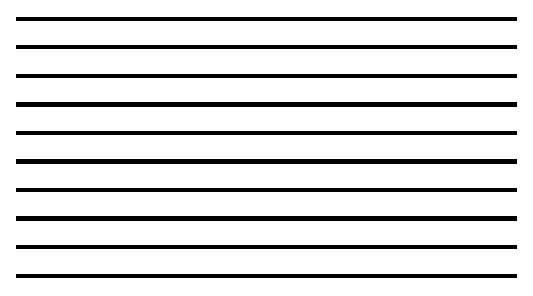
\includegraphics[scale=0.6]{images/parallel-lines.eps}
}

         
\noindent Let's say that the lines are 200 pixels long and that the distance from each line
to the next is 10 pixels, and let's put the start of the first line at the pixel
with coordinates (100,50). To draw one line, we just have to call \code{g.drawLine(x1,y1,x2,y2)}
with appropriate values for the parameters.
Now, all the lines start at \textit{x}-coordinate 100, so we can use the constant 100 as the value for 
\code{x1}.  Since the lines are 200 pixels long, we can use the constant 300 as the value
for \code{x2}.  The \textit{y}-coordinates of the lines are different, but we can see that
both endpoints of a line have the \textbf{same} \textit{y}-coordinates, so we can use a single
variable as the value for \code{y1} and for \code{y2}.  Using \code{y} as the
name of that variable, the command for drawing one of the lines becomes
\code{g.drawLine(100,y,300,y)}.  The value of \code{y} is 50 for the top line
and increases by 10 each time we move down from one line to the next.  We just need to make
sure that \code{y} takes on the correct sequence of values.  We can use a for loop
that counts from 1 to 10:

\displaycode{int y;   // y-coordinate for the line
int i;   // loop control variable
y = 50;  // y starts at 50 for the first line
for ( i = 1; i \<= 10; i++ ) \{
    g.drawLine( 100, y, 300, y );
    y = y + 10;  // increase y by 10 before drawing the next line.
\}}\donedisplaycode


\noindent Alternatively, we could use \code{y} itself as the loop control variable, noting
that the value of \code{y} for the last line is 140:

\displaycode{int y;
for ( y = 50; y \<= 140; y = y + 10 )
    g.drawLine( 100, y, 300, y );}\donedisplaycode


\noindent If we wanted to set the color of the lines, we could do
that by calling \code{g.setColor()} \textbf{before} drawing them.  If we just draw
the lines without setting the color, they will be black.


For something a little more complicated, let's draw a large number of randomly colored,
randomly positioned, filled circles.  Since we only know a few colors, I will randomly select
the color to be red, green, or blue.  That can be done with a simple switch statement, similar
to the ones in Subsection~\ref{control.6.4}:

\displaycode{switch ( (int)(3*Math.random()) ) \{
    case 0:
        g.setColor( Color.RED );
        break;
    case 1:
        g.setColor( Color.GREEN );
        break;
    case 2:
        g.setColor( Color.BLUE );
        break;
\}}\donedisplaycode





I will choose the center points of the circles at random.
Let's say that the width of the drawing area is given by a variable, \code{width}.  Then
we want a random value in the range \code{0} to \code{width-1} for the horizontal
position of the center.  Similarly, the vertical position of the center will a random value
in the range \code{0} to \code{height-1}.  That leaves the size of the circle to
be determined; I will make the radius of each circle equal to 50 pixels.  We can draw the
circle with a statement of the form \code{g.fillOval(x,y,w,h)}.  However, in this
command, \code{x} and \code{y} are not the coordinates of the center of
the circle; they are the upper left corner of a rectangle drawn around the circle.  To get
values for \code{x} and \code{y}, we have to move back from the center of the
circle by 50 pixels, an amount equal to the radius of the circle.  The parameters \code{w}
and \code{h} give the width and height of the rectangle, which has to be twice the 
radius, or 100 pixels in this case.  Taking all this into account, here is a code
segment for drawing a random circle:

\displaycode{centerX = (int)(width*Math.random());
centerY = (int)(height*Math.random());
g.fillOval( centerX - 50, centerY - 50, 100, 100 );}\donedisplaycode


\noindent This code comes after the color-setting code given above.
In the end, I found that the picture looks better if I also draw a black outline
around each filled circle, so I added this code at the end:

\displaycode{g.setColor( Color.BLACK );
g.drawOval( centerX - 50, centerY - 50, 100, 100 );}\donedisplaycode


\noindent Finally, to get a large number of circles, I put all of the above code into
a \code{for} loop that runs for 500 executions.  Here's a typical drawing from
the program, shown at reduced size:


\par\dumpfigure{
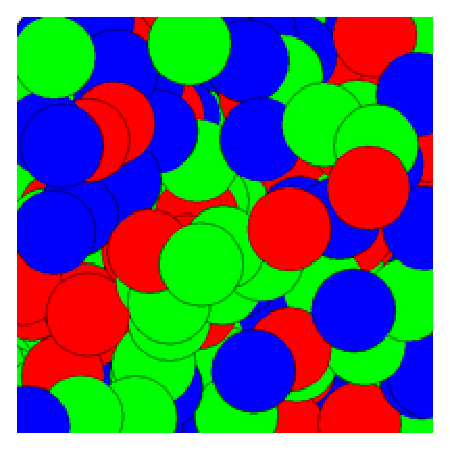
\includegraphics[scale=0.6]{images/random-circles.eps}
}




\subsection{Drawing in a Program}\label{control.8.2}



Now, as you know, you can't just have a bunch of Java code standing by itself.
The code has to be inside a subroutine definition that is itself inside a class
definition.  In fact, for my circle-drawing program, the complete subroutine for
drawing the picture looks like this:

\displaycode{public void drawFrame(Graphics g, int frameNumber, int width, int height) \{
    
    int centerX;     // The x-coord of the center of a disk.
    int centerY;     // The y-coord of the center of a disk.
    int colorChoice; // Used to select a random color.
    int count;       // Loop control variable for counting disks.
    
    for (count = 0; count \< 500; count++) \{
        
        colorChoice = (int)(3*Math.random());
        switch (colorChoice) \{
        case 0:
            g.setColor(Color.RED);
            break;
        case 1:
            g.setColor(Color.GREEN);
            break;
        case 2:
            g.setColor(Color.BLUE);
            break;
        \}
        
        centerX = (int)(width*Math.random());
        centerY = (int)(height*Math.random());
        
        g.fillOval( centerX - 50, centerY - 50, 100, 100 );
        g.setColor(Color.BLACK);
        g.drawOval( centerX - 50, centerY - 50, 100, 100 );
        
    \}
\}}\donedisplaycode


\noindent This is the first subroutine definition that you have seen, other than \code{main()},
but you will learn all about defining subroutines in the next~chapter.
The first line of the definition makes available certain values that are used in the
subroutine:  the graphics context \code{g} and the \code{width} and
\code{height} of the drawing area. (Ignore \code{frameNumber} for now.)  These
values come from outside the subroutine, but the subroutine can use them.  The point here is
that to draw something, you just have to fill in the inside of the subroutine, just
as you write a program by filling in the inside of \code{main()}.


The subroutine definition still has to go inside a class that defines the program.  
In this case, the class is named \classname{RandomCircles}, and the complete
program is available in the sample source code file \sourceref{RandomCircles.java}.
You can run that program to see the drawing.


There's a lot in the program that you won't understand.  To make your own drawing,
all you have to do is erase the inside of the \code{drawFrame()} routine in
the source code and substitute your own drawing code.  You don't need to understand the
rest.  The source code file \sourceref{SimpleAnimationStarter.java} can be
used as a basis for your own first graphics explorations.  It's essentially the same
as \code{RandomCircles.java} but with the drawing code omitted.  You'll need it to do
some of the exercises for this chapter.


(By the way, you might notice that the \code{main()} subroutine uses the word
\code{static} in its definition, but \code{drawFrame()} does not.  This has to
do with the fact that the drawing area in this program is an object, and \code{drawFrame}
is a subroutine in that object.  The difference between static and non-static subroutines
is important but not something that we need to worry about for the time being.  It will become
important for us in Chapter~\ref{OOP}.)



\subsection{Animation}\label{control.8.3}



The name ``SimpleAnimationStarter" should give you a clue that we are looking
at the possibility of more than just individual drawings here.  A computer
animation is simply a sequence of individual pictures, displayed quickly one after
the other.  If the change from each picture to the next is small, the user will perceive the
sequence of images as a continuous animation.  Each picture in the animation is
called a \newword{frame}.  \code{SimpleAnimationStarter.java}
is configured to draw fifty frames every second, although that can be changed.
(In \code{RandomCircles.java}, it has been changed to one frame every three
seconds, so that the program actually draws a new set of random circles every
three seconds.)  The frames in the animation are numbered 0, 1, 2, 3,~\dots,
and the value of \code{frameNumber} in the \code{drawFrame()}
subroutine tells you which frame you are drawing.  The key to programming the
animation is to base what you draw on the \code{frameNumber}.


As an example of animation, we look at drawing a set of nested rectangles.
The rectangles will shrink towards the center of the drawing, giving an illusion of
infinite motion.  Here's one frame from the animation:


\par\dumpfigure{
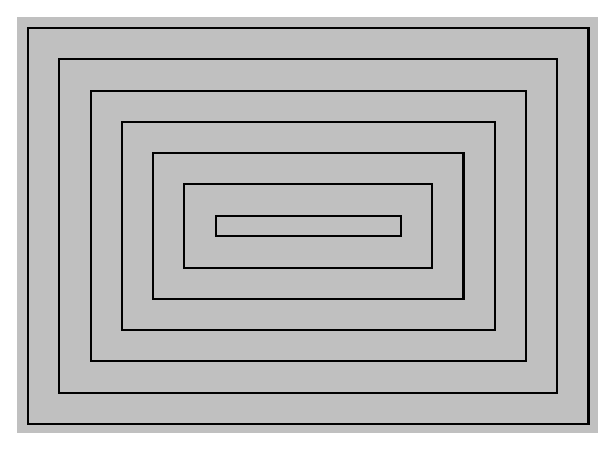
\includegraphics[scale=0.6]{images/moving-rects.eps}
}



Consider how to draw a picture like this one.
The rectangles can be drawn with a \code{while} loop, which draws the rectangles 
starting from the one on the outside and moving in.  Think about what variables will
be needed and how they change from one iteration of the while loop to the next.
Each time through the loop, the rectangle that is drawn is smaller
than the previous one and is moved down and over a bit.  The difference between two rectangles
is in their size and in the coordinates of the upper left corner.  We need a variable to
represent the \code{size}.  The x and y-coordinates are the same, and they can be represented by
the same variable.  I call that variable \code{inset}, since it is the amount by
which the edges of the rectangle are inset from the edges of the drawing area.   The
\code{size} decreases from one rectangle to the next, while the \code{inset}
increases.  The while loop ends when \code{size} becomes less than or equal to zero. 
In general outline, the algorithm for drawing one frame is

\displaycode{Set the drawing color to light gray  (using the g.setColor subroutine)
Fill in the entire picture (using the g.fillRect subroutine)
Set the drawing color to black
Set the amount of inset for the first rectangle
Set the rectangle width and height for the first rectangle
while the width and height are both greater than zero:
    draw a rectangle (using the g.drawRect subroutine)
    increase the inset (to move the next rectangle over and down)
    decrease width the height (the make the next rectangle smaller)}\donedisplaycode


\noindent In my program, each rectangle is 15 pixels away from the rectangle that
surrounds it, so the \code{inset} is increased by 15 each time through the
\code{while} loop.  The rectangle shrinks by 15 pixels on the left
\textbf{and} by 15 pixels on the right, so the width of the rectangle
shrinks by \textbf{30} before drawing the next rectangle. 
The height also shrinks by 30 pixels each time through the loop.


The pseudocode is then easy to translate into Java, except that we
need to know what initial values to use for the inset, width, and height of the
first rectangle.  To figure that out, we have to think about the fact that the picture is
animated, so that what we draw will depend in some way on the frame number.
From one frame to the next frame of the animation, the top-left corner of the outer rectangle moves
over and down; that is, the \code{inset} for the outer rectangle increase from
one frame to the next. We can make this happen by setting
the inset for frame number 0 to 0, the
inset for frame number 1 to 1, and so on.  But that can't go on forever, or eventually
all the rectangles would disappear.  In fact, when the animation gets to frame 15,
a new rectangle should appear at the outside of the drawing area---but it's
not really a ``new rectangle," it's just that the \code{inset} for the outer rectangle
goes back to zero.  So, as
the animation proceeds, the inset should go through the sequence of values
0, 1, 2, \dots, 14 over and over.  We can accomplish that very easily by setting

\displaycode{inset = frameNumber \% 15;}\donedisplaycode


\noindent Finally, note that the first rectangle fills the drawing area except for a border
of size \code{inset} around the outside of the rectangle.  This means that the
the width of the rectangle is the width of the drawing area minus two times the inset,
and similarly for the height.  Here, then is the \code{drawFrame()} subroutine for
the moving rectangle example:

\displaycode{public void drawFrame(Graphics g, int frameNumber, int width, int height) \{

    int inset; // Gap between edges of drawing area and the outer rectangle.

    int rectWidth, rectHeight;   // The size of one of the rectangles.

    g.setColor(Color.LIGHT\_GRAY);
    g.fillRect(0,0,width,height);  // Fill drawing area with light gray.

    g.setColor(Color.BLACK);  // Draw the rectangles in black.

    inset = frameNumber \% 15;  // inset for the outer rectangle

    rectWidth = width - 2*inset;   // drawing area width minus two insets
    rectHeight = height - 2*inset; // drawing area height minus two insets

    while (rectWidth \>= 0 \&\& rectHeight \>= 0) \{
        g.drawRect(inset, inset, rectWidth, rectHeight);
        inset += 15;       // rectangles are 15 pixels apart
        rectWidth -= 30;
        rectHeight -= 30;
    \}
\}}\donedisplaycode

   
\noindent You can find the full source code for the program is in the sample program
\sourceref{MovingRects.java}.





      

   



\begin{exercises}

\exercise 
How many times do you have
to roll a pair of dice before they come up snake eyes? You could do the
experiment by rolling the dice by hand. Write a computer program that simulates
the experiment. The program should report the number of rolls that it makes
before the dice come up snake eyes. (Note: ``Snake eyes" means that both dice
show a value of 1.) Exercise~2.2 explained how to simulate rolling a pair of dice.

\exercise 
Which integer between 1
and 10000 has the largest number of divisors, and how many divisors does it
have? Write a program to find the answers and print out the results. It is
possible that several integers in this range have the same, maximum number of
divisors. Your program only has to print out one of them.  An example in
Subsection~\ref{control.4.2} discussed divisors. The source code for
that example is \sourceref{CountDivisors.java}.


You might need some hints about how to find a maximum value. The basic idea
is to go through all the integers, keeping track of the largest number of
divisors that you've seen \textit{so far}. Also, keep track of the integer that
had that number of divisors.

\exercise 
Write a program that will
evaluate simple expressions such as 17 + 3 and 3.14159 * 4.7. The expressions
are to be typed in by the user. The input always consists of a number, followed
by an operator, followed by another number. The operators that are allowed are
+, -, *, and /. You can read the numbers with \code{TextIO.getDouble()} and
the operator with \code{TextIO.getChar()}. Your program should read an
expression, print its value, read another expression, print its value, and so
on. The program should end when the user enters 0 as the first number on the
line.

\exercise 
Write a program that reads
one line of input text and breaks it up into words. The words should be output
one per line. A word is defined to be a sequence of letters. Any characters in
the input that are not letters should be discarded. For example, if the user
inputs the line

\displaycode{He said, "That's not a good idea."}\donedisplaycode


\noindent then the output of the program should be

\displaycode{He
said
That
s
not
a
good
idea}\donedisplaycode


\noindent An improved version of the program would list ``that's" as a single word. An
apostrophe can be considered to be part of a word if there is a letter on each
side of the apostrophe.


To test whether a character is a letter, you might use \code{(ch \>= 'a'
\&\& ch \<= 'z') || (ch \>= 'A' \&\& ch \<= 'Z')}.
However, this only works in English and similar languages. A better choice is
to call the standard function \code{Character.isLetter(ch)}, which returns a
boolean value of \code{true} if \code{ch} is a letter and \code{false} if
it is not. This works for any Unicode character.

\exercise 
Suppose that a file contains information about sales 
figures for a company in various cities.
Each line of the file contains a city name, followed by a colon~(:) followed by the data for that
city.  The data is a number of type \ptype{double.}
However, for some cities, no data was available.  In these lines, the data is replaced by
a comment explaining why the data is missing.  For example, several lines from the file might
look like:
\displaycode{San Francisco:  19887.32
Chicago:  no report received
New York: 298734.12}\donedisplaycode

\noindent Write a program that will compute and print the total sales from all the cities together. The
program should also report the number of cities for which data was not available.  The name of the
file is ``sales.dat".

To complete this program, you'll need one fact about file input with \classname{TextIO}
that was not covered in Subsection~\ref{basics.4.4}.  Since you don't know in advance how many
lines there are in the file, you need a way to tell when you have gotten to the end of the file.
When \classname{TextIO} is reading from a file, the function \code{TextIO.eof()}
can be used to test for \newword{end of file}.  This \ptype{boolean}-valued
function returns \code{true} if the file has been entirely read and returns \code{false}
if there is more data to read in the file.  This means that you can read the lines of the
file in a loop \code{while~(TextIO.eof()~==~false)\dots}. The loop will end
when all the lines of the file have been read.

Suggestion:  For each line, read and ignore characters up to the colon.  Then read the rest
of the line into a variable of type \classname{String}.  Try to convert the string
into a number, and use \code{try..catch} to test whether the conversion succeeds.

\exercise 
Exercise~3.2 asked you to find the
number in the range 1 to 10000 that has the largest number of divisors.  You
only had to print out one such number.  Revise the program so that it will
print out \textbf{all} numbers that have the maximum number of divisors.  Use an
array as follows:  As you count the divisors for each number, store each
count in an array.  Then at the end of the program, 
you can go through the array and print out all the numbers
that have the maximum count.  The output from the program should look
something like this:
\displaycode{Among integers between 1 and 10000,
The maximum number of divisors was 64
Numbers with that many divisors include:
   7560
   9240}\donedisplaycode


\exercise 
An example in Subsection~\ref{control.7a.3}
tried to answer the question, How many random people
do you have to select before you find a duplicate birthday? The source code for
that program can be found in the file
\sourceref{BirthdayProblem.java}. Here are
some related questions:


\mylist{

\myitem How many random people do you have to select before you find \textbf{three}
people who share the same birthday? (That is, all three people were born on the
same day in the same month, but not necessarily in the same year.)
\myitem Suppose you choose 365 people at random. How many different birthdays will
they have? (The number could theoretically be anywhere from 1 to 365).
\myitem How many different people do you have to check before you've found at least
one person with a birthday on each of the 365 days of the year?
}


Write \textbf{three} programs to answer these questions. Each of your programs should simulate
choosing people at random and checking their birthdays. (In each case, ignore
the possibility of leap years.)

\exercise 
Write a GUI program that draws
a checkerboard.  Base your solution on the sample program
\sourceref{SimpleAnimationStarter.java}, even though you are
creating only a static picture rather than an animation.  You will draw
the checkerboard in the \code{drawFrame()} subroutine.  You should
read the comments in the file to discover other changes that you might
need to make.


Assume that the size of the drawing area is 400-by-400  pixels.  A checkerboard
contains 8 rows and 8 columns of squares.  If the size of the drawing area is 400,
that means that each square can be 50-by-50 pixels.  
The squares are red and black (or whatever other colors you choose). Here is a tricky way
to determine whether a given square should be red or black: The rows and columns can be
thought of as numbered from 0 to 7.  If the row number of the square and the
column number of the square are either both even or both odd, then the square is red.
Otherwise, it is black. Note that a square is just a rectangle in which the
height is equal to the width, so you can use the subroutine
\code{g.fillRect()} to draw the squares. Here is a reduced-size image of the
checkerboard that you want to draw:


\par\dumpfigure{
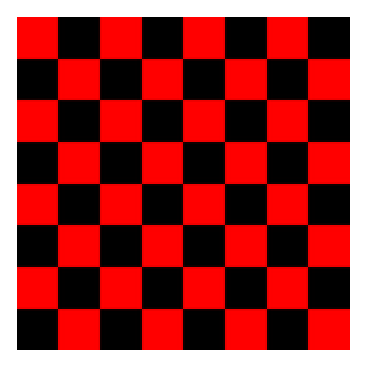
\includegraphics{images/checkerboard.eps}
}



\exercise 
Often, some element of an animation repeats over and over, every so many frames.
Sometimes, the repetition is ``cyclic,"  meaning that at the end it jumps back to the start.
Sometimes the repetition is ``oscillating," like a back-and-forth motion where the second
half is the same as the first half played in reverse.

Write an animation that demonstrates both cyclic and oscillating motions at various speeds.
For cyclic motion, you can use a square that moves across the drawing area, then jumps back to
the start, and then repeats the same motion over and over.  For oscillating motion, you can do something
similar, but the square should move back and forth between the two edges of the drawing area; that is,
it moves left-to-right during the first half of the animation and then backwards from right-to-left
during the second half.  To write the program, you can start with a copy of
the sample program \sourceref{SimpleAnimationStarter.java}, as in the previous exercise.

A cyclic motion has to repeat every N frames for some value of N.  What you draw in some
frame of the animation depends on the \code{frameNumber}.  The \code{frameNumber} just keeps
increasing forever.  To implement cyclic motion, what you really want is a ``cyclic frame number" that
takes on the values 0, 1, 2, \dots, (N-1), 0, 1, 2, \dots, (N-1), 0, 1, 2, \dots.  You can derive
the value that you need from \code{frameNumber} simply by saying
\displaycode{cyclicFrameNumber = frameNumber \% N;}\donedisplaycode

\noindent Then, you just have to base what you draw on \code{cyclicFrameNumber} instead of on
\code{frameNumber}.  Similarly, for an oscillating animation, you need an
``oscillation frame number" that takes on the values  0, 1, 2, \dots (N-1), N, (N-1), (N-2), \dots 2, 1, 0, 1, 2, 
and so on, repeating the back and forth motion forever.  You can compute the value that you need with
\displaycode{oscilationFrameNumber = frameNumber \% (2*N);
if (oscillationFrameNumber \> N)
   oscillationFrameNumber = (2*N) - oscillationFrameNumber;}\donedisplaycode


Here is a screen shot from my version of the program.  I use
six squares.  The top three do cyclic motion at various speeds, while the bottom three do
oscillating motion.  I drew black lines across the drawing area to separate the squares and to give
them ``channels" to move in.


\par\dumpfigure{
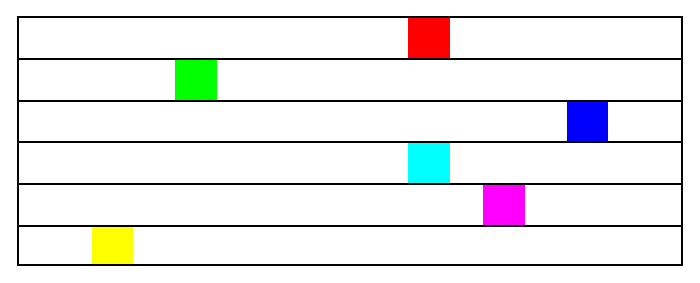
\includegraphics[scale=0.8]{images/motion-demo.eps}
}

 

\end{exercises}

   



\begin{quiz}

\quizquestion 
What is an \textit{algorithm}?
\quizquestion 
Explain briefly what is
meant by ``pseudocode" and how is it useful in the development of
algorithms.
\quizquestion 
What is a \textit{block
statement?} How are block statements used in Java programs?
\quizquestion 
What is the main difference
between a \code{while} loop and a \code{do..while} loop?
\quizquestion 
What does it mean to
\textit{prime} a loop?
\quizquestion 
Explain what is meant by an
\textit{animation} and how a computer displays an animation.
\quizquestion 
Write a \code{for} loop
that will print out all the multiples of 3 from 3 to 36, that is: 3 6 9 12 15
18 21 24 27 30 33 36.
\quizquestion 
Fill in the following
\code{main()} routine so that it will ask the user to enter an integer, read
the user's response, and tell the user whether the number entered is even or
odd. (You can use \code{TextIO.getInt()} to read the integer. Recall that an
integer \code{n} is even if \code{n~\%~2~==~0}.)
\displaycode{public static void main(String[] args) \{
 
         // Fill in the body of this subroutine!
 
\}}\donedisplaycode


\quizquestion 
Write a code segment that will print out two \textit{different} random integers
selected from the range 1 to 10.  All possible outputs should have the same probability.
Hint:  You can easily select two random numbers, but you have to account for the
fact that the two numbers that you pick might be the same.

\quizquestion 
Suppose that \code{s1} and \code{s2} are variables of type
\classname{String}, whose values are expected to be string representations
of values of type \ptype{int}.  Write a code segment that will compute and print
the integer sum of those values, or will print an error message if the values cannot
successfully be converted into integers.  (Use a \code{try..catch} statement.)
\quizquestion 
Show the exact output that
would be produced by the following \code{main()} routine:
\displaycode{public static void main(String[] args) \{
    int N;
    N = 1;
    while (N \<= 32) \{
       N = 2 * N;
       System.out.println(N);   
    \}
\}}\donedisplaycode


\quizquestion 
Show the exact output
produced by the following \code{main()} routine:
\displaycode{public static void main(String[] args) \{
   int x,y;
   x = 5;
   y = 1;
   while (x \> 0) \{
      x = x - 1;
      y = y * x;
      System.out.println(y);
   \}
\}}\donedisplaycode


\quizquestion 
What output is produced by
the following program segment? \textbf{Why?} (Recall that \code{name.charAt(i)}
is the i-th character in the string, \code{name}.)
\displaycode{String name;
int i;
boolean startWord;

name = "Richard M. Nixon";
startWord = true;
for (i = 0; i \< name.length(); i++) \{
   if (startWord)
      System.out.println(name.charAt(i));
   if (name.charAt(i) == ' ')
      startWord = true;
   else
      startWord = false;
\}}\donedisplaycode


\quizquestion 
Suppose that \code{numbers} is an array of type \atype{int\hbox{[\hskip2pt]}}.
Write a code segment that will count and output the number of times that the
number 42 occurs in the array.

\quizquestion 
Define the \newword{range} of an array of numbers to be
the maximum value in the array minus the minimum value.  Suppose that
\code{raceTimes} is an array of type \atype{double\hbox{[\hskip2pt]}}.
Write a code segment that will find and print the range of \code{raceTimes}.


\end{quiz}


\chapter[Subroutines]{Programming in the Large I:\\ Subroutines}\label{subroutines}
 
   





\start{{\Large O}ne way to break up a complex program} into
manageable pieces is to use \newword{subroutines}. A
subroutine consists of the instructions for carrying out a certain task,
grouped together and given a name. Elsewhere in the program, that name can be
used as a stand-in for the whole set of instructions. As a computer executes a
program, whenever it encounters a subroutine name, it executes all the
instructions necessary to carry out the task associated with that
subroutine.


Subroutines can be used over and over, at different places in the program. A
subroutine can even be used inside another subroutine. This allows you to write
simple subroutines and then use them to help write more complex subroutines,
which can then be used in turn in other subroutines. In this way, very complex
programs can be built up step-by-step, where each step in the construction is
reasonably simple.


Subroutines in Java can be either static or non-static. This chapter 
covers static subroutines. Non-static subroutines, which are used in 
true object-oriented programming, will be covered in the next chapter.


   



\section{Black Boxes}\label{subroutines.1}

   

\start{{\Large A} subroutine consists of instructions} for
performing some task, chunked together and given a name. ``Chunking" allows you
to deal with a potentially very complicated task as a single concept. Instead
of worrying about the many, many steps that the computer might have to go
though to perform that task, you just need to remember the name of the
subroutine. Whenever you want your program to perform the task, you just call
the subroutine. Subroutines are a major tool for dealing with complexity.


A subroutine is sometimes said to be a ``black box" because you can't see
what's ``inside" it (or, to be more precise, you usually don't
\textbf{want} to see inside it, because then you would have to deal
with all the complexity that the subroutine is meant to hide). Of course, a
black box that has no way of interacting with the rest of the world would be
pretty useless. A black box needs some kind of \newword{interface} 
with the rest of the world, which allows some
interaction between what's inside the box and what's outside. A physical black
box might have buttons on the outside that you can push, dials that you can
set, and slots that can be used for passing information back and forth. Since
we are trying to hide complexity, not create it, we have the first rule of
black boxes:


\medbreak
{\advance \leftskip by 70 pt \advance \rightskip by 70 pt



\textbf{The interface of a black box should be fairly straightforward,
well-defined, and easy to understand.}



}
\medbreak



Are there any examples of black boxes in the real world? Yes; in fact, you
are surrounded by them. Your television, your car, your mobile phone, your
refrigerator\dots. You can turn your television on and off, change channels, and
set the volume by using elements of the television's interface---dials, remote
control, don't forget to plug in the power---without understanding anything
about how the thing actually works. The same goes for a mobile phone, although
the interface in that case is a lot more complicated.


Now, a black box does have an inside---the code in a subroutine that
actually performs the task, or all the electronics inside your television set. The
inside of a black box is called its \newword{implementation}. 
The second rule of black boxes is that:


\medbreak
{\advance \leftskip by 70 pt \advance \rightskip by 70 pt



\textbf{To use a black box, you shouldn't need to know anything about its
implementation; all you need to know is its interface.}



}
\medbreak



In fact, it should be possible to \textbf{change} the
implementation, as long as the behavior of the box, as seen from the outside,
remains unchanged. For example, when the insides of TV sets went from using
vacuum tubes to using transistors, the users of the sets didn't need to
know about it---or even know what it means. Similarly, it should be possible
to rewrite the inside of a subroutine, to use more efficient code, for example,
without affecting the programs that use that subroutine.


Of course, to have a black box, someone must have designed and built the
implementation in the first place. The black box idea works to the advantage of
the implementor as well as the user of the black box. After all, the black
box might be used in an unlimited number of different situations. The
implementor of the black box doesn't need to know about any of that. The
implementor just needs to make sure that the box performs its assigned task and
interfaces correctly with the rest of the world. This is the third rule of
black boxes:


\medbreak
{\advance \leftskip by 70 pt \advance \rightskip by 70 pt



\textbf{The implementor of a black box should not need to know anything about the
larger systems in which the box will be used.}



}
\medbreak



In a way, a black box divides the world into two parts: the inside
(implementation) and the outside. The interface is at the boundary, connecting
those two parts.


\mybreak



By the way, you should \textbf{not} think of an interface as just
the physical connection between the box and the rest of the world. The
interface also includes a \newword{specification} of what
the box does and how it can be controlled by using the elements of the physical
interface. It's not enough to say that a TV set has a power switch; you need to
specify that the power switch is used to turn the TV on and off!


To put this in computer science terms, the interface of a subroutine has a
semantic as well as a syntactic component. The syntactic part of the interface
tells you just what you have to type in order to call the subroutine. The
semantic component specifies exactly what task the subroutine will accomplish.
To write a legal program, you need to know the syntactic specification of the
subroutine. To understand the purpose of the subroutine and to use it
effectively, you need to know the subroutine's semantic specification. I will
refer to both parts of the interface---syntactic and semantic---collectively
as the \newword{contract} of the subroutine.


The contract of a subroutine says, essentially, ``Here is what you have to do
to use me, and here is what I will do for you, guaranteed." When you write a
subroutine, the comments that you write for the subroutine should make the
contract very clear. (I should admit that in practice, subroutines' contracts
are often inadequately specified, much to the regret and annoyance of the
programmers who have to use them.)


For the rest of this chapter, I turn from general ideas about black boxes
and subroutines in general to the specifics of writing and using subroutines in
Java. But keep the general ideas and principles in mind. They are the reasons
that subroutines exist in the first place, and they are your guidelines for
using them. This should be especially clear in Section~\ref{subroutines.6},
where I will discuss subroutines as a tool in program development.


\mybreak



You should keep in mind that subroutines are not the only example of black
boxes in programming. For example, a class is also a black box. We'll see that
a class can have a ``public" part, representing its interface, and a ``private"
part that is entirely inside its hidden implementation. All the principles of
black boxes apply to classes as well as to subroutines.


   



\section[Static Subroutines and Variables]{Static Subroutines and Static Variables}\label{subroutines.2}



\start{{\Large E}very subroutine in Java} must be defined inside
some class. This makes Java rather unusual among programming languages, since
most languages allow free-floating, independent subroutines. One purpose of a
class is to group together related subroutines and variables. Perhaps the
designers of Java felt that everything must be related to something. As a less
philosophical motivation, Java's designers wanted to place firm controls on the
ways things are named, since a Java program potentially has access to a huge
number of subroutines created by many different programmers. The fact that those
subroutines are grouped into named classes (and classes are grouped into named
``packages," as we will see later) helps control the confusion that might result from so many
different names.


There is a basic distinction in Java between \newword{static} and
\newword{non-static} subroutines.  A class definition can contain the
source code for both types of subroutine, but what's done with them when the
program runs is very different.  Static subroutines are easier to understand:
In a running program, a static subroutine is a member of the class itself.
Non-static subroutine definitions, on the other hand, are only there to be used
when objects are created, and the subroutines themselves become members of the
objects.  Non-static subroutines only become relevant when you are working 
with objects.  The distinction between static and non-static also applies to variables
and to other things that can occur in class definitions.  This chapter will
deal with static subroutines and static variables almost exclusively. We'll turn to non-static
stuff and to object-oriented programming in the next
chapter.


A subroutine that is in a class or object is often called a \newword{method}, 
and ``method" is the term that most people prefer for
subroutines in Java. I will start using the term ``method" occasionally;
however, I will continue to prefer the more general term ``subroutine" 
in this chapter, at least for static subroutines.  However, you should start
thinking of the terms ``method" and ``subroutine" as being essentially
synonymous as far as Java is concerned.

\subsection{Subroutine Definitions}\label{subroutines.2.1}



A subroutine must be defined somewhere.  The definition has to include the name of the subroutine,
enough information to make it possible to call the subroutine, and the code that will be executed
each time the subroutine is called.  A subroutine definition in Java takes the form:

\displaycode{\bnf{modifiers}  \bnf{return-type}  \bnf{subroutine-name}  ( \bnf{parameter-list} ) \{
    \bnf{statements}
\}}\donedisplaycode


\noindent It will take us a while---most of the chapter---to get through what all
this means in detail. Of course, you've already seen examples of subroutines in
previous chapters, such as the \code{main()} routine of a program and the
\code{drawFrame()} routine of the animation programs in Section~\ref{control.8}. 
So you are familiar with the general format.


The \bnf{statements} between the braces, \{ and \}, in a subroutine definition
make up the \newword{body} of the subroutine. These
statements are the inside, or implementation part, of the ``black box," as
discussed in the previous section. They are the
instructions that the computer executes when the method is called. Subroutines
can contain any of the statements discussed in Chapter~\ref{basics} and
Chapter~\ref{control}.


The \bnf{modifiers} that can occur at the
beginning of a subroutine definition are words that set certain characteristics
of the subroutine, such as whether it is static or not. The modifiers that you've
seen so far are ``\code{static}" and ``\code{public}". There are only about a
half-dozen possible modifiers altogether.


If the subroutine is a function, whose job is to compute some value, then
the \bnf{return-type} is used to specify the type of
value that is returned by the function.  It can be a type name such as
\classname{String} or \ptype{int} or even an array type
such as \atype{double\hbox{[\hskip2pt]}}.  We'll be looking at functions and
return types in some detail in Section~\ref{subroutines.4}. If the
subroutine is not a function, then the \bnf{return-type} is replaced 
by the special value \code{void},
which indicates that no value is returned. The term ``void" is meant to indicate
that the return value is empty or non-existent.


Finally, we come to the \bnf{parameter-list} of
the method. Parameters are part of the interface of a subroutine. They
represent information that is passed into the subroutine from outside, to be
used by the subroutine's internal computations. For a concrete example, imagine
a class named \classname{Television} that includes a method named
\code{changeChannel()}. The immediate question is: What channel should it
change to? A parameter can be used to answer this question. Since the channel
number is an integer, the type of the parameter would be \ptype{int}, and the
declaration of the \code{changeChannel()} method might look like

\displaycode{public void changeChannel(int channelNum) \{ ... \}}\donedisplaycode


\noindent This declaration specifies that \code{changeChannel()} has a parameter
named \code{channelNum} of type \ptype{int}. However, \code{channelNum}
does not yet have any particular value. A value for \code{channelNum} is
provided when the subroutine is called; for example:
\code{changeChannel(17);}


The parameter list in a subroutine can be empty, or it can consist of one or
more parameter declarations of the form \bnf{type}~\bnf{parameter-name}. If there are several
declarations, they are separated by commas. Note that each declaration can name
only one parameter. For example, if you want two parameters of type
\ptype{double}, you have to say ``\code{double~x,~double~y}", rather than
``\code{double x, y}".


Parameters are covered in more detail in the next
section.


Here are a few examples of subroutine definitions, leaving out the
statements that define what the subroutines do:

\displaycode{public static void playGame() \{
    // "public" and "static" are modifiers; "void" is the 
    // return-type; "playGame" is the subroutine-name; 
    // the parameter-list is empty.
    . . .  // Statements that define what playGame does go here.
\}

int getNextN(int N) \{
    // There are no modifiers; "int" in the return-type;
    // "getNextN" is the subroutine-name; the parameter-list 
    // includes one parameter whose name is "N" and whose 
    // type is "int".
    . . .  // Statements that define what getNextN does go here.
\}

static boolean lessThan(double x, double y) \{
    // "static" is a modifier; "boolean" is the
    // return-type; "lessThan" is the subroutine-name; 
    // the parameter-list includes two parameters whose names are 
    // "x" and "y", and the type of each of these parameters 
    // is "double".
    . . .  // Statements that define what lessThan does go here.
\}}\donedisplaycode



In the second example given here, \code{getNextN} is a non-static method,
since its definition does not include the modifier ``\code{static}"---and so
it's not an example that we should be looking at in this chapter! The other
modifier shown in the examples is ``\code{public}". This modifier indicates
that the method can be called from anywhere in a program, even from outside the
class where the method is defined. There is another modifier,
``\code{private}", which indicates that the method can be called
\textbf{only} from inside the same class. The modifiers \code{public}
and \code{private} are called \newword{access specifiers}.
If no access specifier is given for a method, then by default, that method can
be called from anywhere in the ``package" that contains the class, but not from
outside that package. (Packages were mentioned in Subsection~\ref{basics.6.6},
and you'll learn more about them later in this
chapter, in Section~\ref{subroutines.5}.)  There is one other access
modifier, \code{protected}, which will only become relevant when we turn to
object-oriented programming in Chapter~\ref{OOP}.


Note, by the way, that the \code{main()} routine of a program follows the
usual syntax rules for a subroutine. In

\displaycode{public static void main(String[] args) \{ ... \}}\donedisplaycode


\noindent the modifiers are \code{public} and \code{static}, the return type is
\code{void}, the subroutine name is \code{main}, and the parameter list is
``\code{String[]~args}".  In this case, the type for the parameter is
the array type \atype{String\hbox{[\hskip2pt]}}.


You've already had some experience with filling in the implementation of a
subroutine. In this chapter, you'll learn all about writing your own complete
subroutine definitions, including the interface part.


   
\subsection{Calling Subroutines}\label{subroutines.2.2}



When you define a subroutine, all you are doing is telling the computer that
the subroutine exists and what it does. The subroutine doesn't actually get
executed until it is called. (This is true even for the \code{main()} routine
in a class---even though \textbf{you} don't call it, it is called by
the system when the system runs your program.) For example, the
\code{playGame()} method given as an example above could be called using the following
subroutine call statement:

\displaycode{playGame();}\donedisplaycode


\noindent This statement could occur anywhere in the same class that includes the
definition of \code{playGame()}, whether in a \code{main()} method or in
some other subroutine. Since \code{playGame()} is a \code{public} method,
it can also be called from other classes, but in that case, you have to tell
the computer which class it comes from.  Since \code{playGame()} is a \code{static} method,
its full name includes the name of the class in which it is defined.  Let's say, for example, that
\code{playGame()} is defined in a class named \code{Poker}. Then to call
\code{playGame()} from \textbf{outside} the \code{Poker} class, you would
have to say

\displaycode{Poker.playGame();}\donedisplaycode


\noindent The use of the class name here tells the computer which class to look in to
find the method.  It also lets you distinguish between \code{Poker.playGame()}
and other potential \code{playGame()} methods defined in other classes, such
as \code{Roulette.playGame()} or \code{Blackjack.playGame()}.


More generally, a \newword{subroutine call statement} for a \code{static}
subroutine takes the form

\displaycode{\bnf{subroutine-name}(\bnf{parameters});}\donedisplaycode


\noindent if the subroutine that is being called is in the same class, or

\displaycode{\bnf{class-name}.\bnf{subroutine-name}(\bnf{parameters});}\donedisplaycode


\noindent if the subroutine is defined elsewhere, in a different
class. (Non-static methods belong to objects rather than classes, and they are
called using objects instead of class names. More on that later.) Note
that the parameter list can be empty, as in the \code{playGame()} example,
but the parentheses must be there even if there is nothing between them.
The number of parameters that you provide when you call a subroutine must
match the number listed in the parameter list in the subroutine definition,
and the types of the parameters in the call statement must match the types
in the subroutine definition.


   
\subsection{Subroutines in Programs}\label{subroutines.2.3}



It's time to give an example of what a complete program looks like, when it
includes other subroutines in addition to the \code{main()} routine. Let's
write a program that plays a guessing game with the user. The computer will
choose a random number between 1 and 100, and the user will try to guess it.
The computer tells the user whether the guess is high or low or correct. If the
user gets the number after six guesses or fewer, the user wins the game. After
each game, the user has the option of continuing with another game.


Since playing one game can be thought of as a single, coherent task, it
makes sense to write a subroutine that will play one guessing game with the
user. The \code{main()} routine will use a loop to call the
\code{playGame()} subroutine over and over, as many times as the user wants
to play. We approach the problem of designing the \code{playGame()}
subroutine the same way we write a \code{main()} routine: Start with an
outline of the algorithm and apply stepwise refinement. Here is a short
pseudocode algorithm for a guessing game routine:

\displaycode{Pick a random number
while the game is not over:
    Get the user's guess
    Tell the user whether the guess is high, low, or correct.}\donedisplaycode



The test for whether the game is over is complicated, since the game ends if
either the user makes a correct guess or the number of guesses is six. As in
many cases, the easiest thing to do is to use a ``\code{while~(true)}" loop
and use \code{break} to end the loop whenever we find a reason to do so.
Also, if we are going to end the game after six guesses, we'll have to keep
track of the number of guesses that the user has made. Filling out the
algorithm gives:

\displaycode{Let computersNumber be a random number between 1 and 100
Let guessCount = 0
while (true):
    Get the user's guess
    Count the guess by adding 1 to guess count
    if the user's guess equals computersNumber:
        Tell the user he won
        break out of the loop
    if the number of guesses is 6:
        Tell the user he lost
        break out of the loop
    if the user's guess is less than computersNumber:
        Tell the user the guess was low
    else if the user's guess is higher than computersNumber:
        Tell the user the guess was high}\donedisplaycode



With variable declarations added and translated into Java, this becomes the
definition of the \code{playGame()} routine. A random integer between 1 and
100 can be computed as \code{(int)(100~* Math.random())~+~1}. I've cleaned up
the interaction with the user to make it flow better.

\displaycode{static void playGame() \{
    int computersNumber; // A random number picked by the computer.
    int usersGuess;      // A number entered by user as a guess.
    int guessCount;      // Number of guesses the user has made.
    computersNumber = (int)(100 * Math.random()) + 1;
             // The value assigned to computersNumber is a randomly
             //    chosen integer between 1 and 100, inclusive.
    guessCount = 0;
    System.out.println();
    System.out.print("What is your first guess? ");
    while (true) \{
       usersGuess = TextIO.getInt();  // Get the user's guess.
       guessCount++;
       if (usersGuess == computersNumber) \{
          System.out.println("You got it in " + guessCount
                  + " guesses!  My number was " + computersNumber);
          break;  // The game is over; the user has won.
       \}
       if (guessCount == 6) \{
          System.out.println("You didn't get the number in 6 guesses.");
          System.out.println("You lose.  My number was " + computersNumber);
          break;  // The game is over; the user has lost.
       \}
       // If we get to this point, the game continues.
       // Tell the user if the guess was too high or too low.
       if (usersGuess \< computersNumber)
          System.out.print("That's too low.  Try again: ");
       else if (usersGuess \> computersNumber)
          System.out.print("That's too high.  Try again: ");
    \}
    System.out.println();
\} // end of playGame()}\donedisplaycode



Now, where exactly should you put this? It should be part of the same class
as the \code{main()} routine, but \textbf{not} inside the main routine. It is not
legal to have one subroutine physically nested inside another. The
\code{main()} routine will \textbf{call} \code{playGame()}, but not contain
its definition, only a call statement. You can put the definition of \code{playGame()} either before
or after the \code{main()} routine. Java is not very picky about having the
members of a class in any particular order.


It's pretty easy to write the main routine. You've done things like this
before. Here's what the complete program looks like (except that a serious
program needs more comments than I've included here).

\displaycode{public class GuessingGame \{

   public static void main(String[] args) \{
      System.out.println("Let's play a game.  I'll pick a number between");
      System.out.println("1 and 100, and you try to guess it.");
      boolean playAgain;
      do \{
         playGame();  // call subroutine to play one game
         System.out.print("Would you like to play again? ");
         playAgain = TextIO.getlnBoolean();
      \} while (playAgain);
      System.out.println("Thanks for playing.  Goodbye.");
   \} // end of main()            
   
   static void playGame() \{
       int computersNumber; // A random number picked by the computer.
       int usersGuess;      // A number entered by user as a guess.
       int guessCount;      // Number of guesses the user has made.
       computersNumber = (int)(100 * Math.random()) + 1;
                // The value assigned to computersNumber is a randomly
                //    chosen integer between 1 and 100, inclusive.
       guessCount = 0;
       System.out.println();
       System.out.print("What is your first guess? ");
       while (true) \{
          usersGuess = TextIO.getInt();  // Get the user's guess.
          guessCount++;
          if (usersGuess == computersNumber) \{
             System.out.println("You got it in " + guessCount
                     + " guesses!  My number was " + computersNumber);
             break;  // The game is over; the user has won.
          \}
          if (guessCount == 6) \{
             System.out.println("You didn't get the number in 6 guesses.");
             System.out.println("You lose.  My number was " + computersNumber);
             break;  // The game is over; the user has lost.
          \}
          // If we get to this point, the game continues.
          // Tell the user if the guess was too high or too low.
          if (usersGuess \< computersNumber)
             System.out.print("That's too low.  Try again: ");
          else if (usersGuess \> computersNumber)
             System.out.print("That's too high.  Try again: ");
       \}
       System.out.println();
   \} // end of playGame()
               
\} // end of class GuessingGame}\donedisplaycode



Take some time to read the program carefully and figure out how it works.
And try to convince yourself that even in this relatively simple case, breaking
up the program into two methods makes the program easier to understand and
probably made it easier to write each piece.


\subsection{Member Variables}\label{subroutines.2.4}



A class can include other things besides subroutines. In particular, it can
also include variable declarations. Of course, you can declare variables
\textbf{inside} subroutines.  Those are called \newword{local variables.} 
However, you can also have variables that are
not part of any subroutine. To distinguish such variables from local variables,
we call them \newword{member variables}, since they are
members of a class.  Another term for them is \newword{global variable}.


Just as with subroutines, member variables can be either static or
non-static. In this chapter, we'll stick to static variables. A static member
variable belongs to the class as a whole, and it exists as long as the class
exists. Memory is allocated for the variable when the class is first loaded by
the Java interpreter. Any assignment statement that assigns a value to the
variable changes the content of that memory, no matter where that assignment
statement is located in the program. Any time the variable is used in an
expression, the value is fetched from that same memory, no matter where the
expression is located in the program. This means that the value of a static
member variable can be set in one subroutine and used in another subroutine.
Static member variables are ``shared" by all the static subroutines in the
class. A local variable in a subroutine, on the other hand, exists only while
that subroutine is being executed, and is completely inaccessible from outside
that one subroutine.


The declaration of a member variable looks just like the declaration of a
local variable except for two things: The member variable is declared outside
any subroutine (although it still has to be inside a class), and the
declaration can be marked with modifiers such as \code{static},
\code{public}, and \code{private}. Since we are only working with static
member variables for now, every declaration of a member variable in this
chapter will include the modifier \code{static}.  They might also
be marked as \code{public} or \code{private}.  For example:

\displaycode{static String usersName;
public static int numberOfPlayers;
private static double velocity, time;}\donedisplaycode



A static member variable that is not declared to be \code{private} can be
accessed from outside the class where it is defined, as well as inside. When it
is used in some other class, it must be referred to with a compound identifier
of the form \bnf{class-name}.\bnf{variable-name}. For example, the \classname{System} class
contains the public static member variable named \code{out}, and you use this
variable in your own classes by referring to \code{System.out}.   Similarly,
\code{Math.PI} is a public static member variable in the \classname{Math}.  If
\code{numberOfPlayers} is a public static member variable in a class named
\code{Poker}, then code in the \code{Poker} class would refer to it
simply as \code{numberOfPlayers}, while code in another class would refer to
it as \code{Poker.numberOfPlayers}.


As an example, let's add a couple static member variable to the
\code{GuessingGame} class that we wrote earlier in this section.
We add a variable named \code{gamesPlayed} to keep track of how
many games the user has played and another variable named \code{gamesWon}
to keep track of the number of games that the user has won.  The variables
are declared as static member variables:

\displaycode{static int gamesPlayed;
static int gamesWon;}\donedisplaycode


\noindent In the \code{playGame()} routine, we always add 1 to \code{gamesPlayed},
and we add 1 to  \code{gamesWon} if the user wins the game. 
At the end of the \code{main()} routine, we print out the values of both variables.
It would be impossible to 
do the same thing with local variables, since both subroutines need to access the variables,
and local variables exist in only one subroutine.


When you declare a local variable in a subroutine, you have to assign a
value to that variable before you can do anything with it. Member variables, on
the other hand are automatically initialized with a default value.  The default
values are the same as those that are used when initializing the elements of an array:
For numeric variables, the default value is zero; for \ptype{boolean} variables, the
default is \code{false}; for \ptype{char} variables, it's the
character that has Unicode code number zero; and for objects, such as
\classname{Strings}, the default initial value is the special value
\code{null}.


Since they are of type \ptype{int}, the static member variables \code{gamesPlayed}
and \code{gamesWon} automatically get zero as their initial value. This
happens to be the correct initial value for a variable that is being used as a
counter. You can, of course, assign a value to a variable at the
beginning of the \code{main()} routine if you are not satisfied with the
default initial value, or if you want to emphasize that you are depending on
the default.


Here's the revised version of \code{GuessingGame.java}. 
The changes from the above version are shown in italic:

\displaycode{public class GuessingGame2 \{
 
    \newcode{static int gamesPlayed;   // The number of games played.
    static int gamesWon;      // The number of games won.}
 
    public static void main(String[] args) \{
       \newcode{gamesPlayed = 0;
       gamesWon = 0;  // This is actually redundant, since 0 is 
                      //                 the default initial value.}
       System.out.println("Let's play a game.  I'll pick a number between");
       System.out.println("1 and 100, and you try to guess it.");
       boolean playAgain;
       do \{
          playGame();  // call subroutine to play one game
          System.out.print("Would you like to play again? ");
          playAgain = TextIO.getlnBoolean();
       \} while (playAgain);
       \newcode{System.out.println();
       System.out.println("You played " + gamesPlayed + " games,");
       System.out.println("and you won " + gamesWon + " of those games.");}
       System.out.println("Thanks for playing.  Goodbye.");
    \} // end of main()            
    
    static void playGame() \{
        int computersNumber; // A random number picked by the computer.
        int usersGuess;      // A number entered by user as a guess.
        int guessCount;      // Number of guesses the user has made.
        \newcode{gamesPlayed++;  // Count this game.}
        computersNumber = (int)(100 * Math.random()) + 1;
                 // The value assigned to computersNumber is a randomly
                 //    chosen integer between 1 and 100, inclusive.
        guessCount = 0;
        System.out.println();
        System.out.print("What is your first guess? ");
        while (true) \{
           usersGuess = TextIO.getInt();  // Get the user's guess.
           guessCount++;
           if (usersGuess == computersNumber) \{
              System.out.println("You got it in " + guessCount
                      + " guesses!  My number was " + computersNumber);
              \newcode{gamesWon++;  // Count this win.}
              break;       // The game is over; the user has won.
           \}
           if (guessCount == 6) \{
              System.out.println("You didn't get the number in 6 guesses.");
              System.out.println("You lose.  My number was " + computersNumber);
              break;  // The game is over; the user has lost.
           \}
           // If we get to this point, the game continues.
           // Tell the user if the guess was too high or too low.
           if (usersGuess \< computersNumber)
              System.out.print("That's too low.  Try again: ");
           else if (usersGuess \> computersNumber)
              System.out.print("That's too high.  Try again: ");
        \}
        System.out.println();
    \} // end of playGame()
                
\} // end of class GuessingGame2}\donedisplaycode



\mybreak



(By the way, notice that in my example programs, I didn't mark the static subroutines
or variables as being \code{public} or \code{private}.  You might wonder what
it means to leave out both modifiers. Recall that global variables and subroutines 
with no access modifier
can be used anywhere in the same package as the class where they are defined, but not in
other packages. Classes that
don't declare a package are in the default package.  So, any class in the default package
would have access to \code{gamesPlayed}, \code{gamesWon}, and
\code{playGame()}---and that includes pretty much every class in this book.  In fact,
it is considered to be good practice 
to make member variables and subroutines \code{private}, unless
there is a reason for doing otherwise.)
 
 

   



\section{Parameters}\label{subroutines.3}



\start{{\Large I}f a subroutine is a black box}, then a parameter
is something that
provides a mechanism for passing information from the outside world into the
box. Parameters are part of the interface of a subroutine. They allow you to
customize the behavior of a subroutine to adapt it to a particular
situation.


As an analogy, consider a thermostat---a black box whose task it is to keep
your house at a certain temperature. The thermostat has a parameter, namely the
dial that is used to set the desired temperature. The thermostat always
performs the same task: maintaining a constant temperature. However, the exact
task that it performs---that is, \textbf{which} temperature it
maintains---is customized by the setting on its dial.
   
\subsection{Using Parameters}\label{subroutines.3.1}



As an example, let's go back to the ``3N+1" problem that was discussed in
Subsection~\ref{control.2.2}. (Recall that a 3N+1 sequence is
computed according to the rule, ``if N is odd, multiply it by 3 and add 1; if N is
even, divide it by 2; continue until N is equal to 1." For example, starting from
N=3 we get the sequence: 3, 10, 5, 16, 8, 4, 2, 1.) Suppose that we want to
write a subroutine to print out such sequences. The subroutine will always
perform the same task: Print out a 3N+1 sequence. But the exact sequence it
prints out depends on the starting value of N. So, the starting value of N
would be a parameter to the subroutine. The subroutine can be written like
this:

\displaycode{/**
 * This subroutine prints a 3N+1 sequence to standard output, using
 * startingValue as the initial value of N.  It also prints the number 
 * of terms in the sequence. The value of the parameter, startingValue, 
 * must  be a positive integer.
 */

static void print3NSequence(int startingValue) \{
      
   int N;      // One of the terms in the sequence.
   int count;  // The number of terms.
  
   N = startingValue;  // The first term is whatever value
                       //    is passed to the subroutine as 
                       //    a parameter.
   
   count = 1; // We have one term, the starting value, so far.
   
   System.out.println("The 3N+1 sequence starting from " + N);
   System.out.println();
   System.out.println(N);  // print initial term of sequence
 
   while (N \> 1) \{
       if (N \% 2 == 1)     // is N odd?
          N = 3 * N + 1;
       else
          N = N / 2;
       count++;   // count this term
       System.out.println(N);  // print this term
   \}
   
   System.out.println();
   System.out.println("There were " + count + " terms in the sequence.");

\}  // end print3NSequence}\donedisplaycode


\noindent The parameter list of this subroutine, ``\code{(int~startingValue)}",
specifies that the subroutine has one parameter, of type \ptype{int}.   Within
the body of the subroutine, the parameter name can be used in the same way as a
variable name.  But notice that there is nothing in the subroutine definition that
gives a value to the parameter!
The parameter gets its initial value from \textbf{outside} the subroutine.  When the
subroutine is called, a value must be provided for the parameter in the subroutine call 
statement.  This value
will be assigned to \code{startingValue} before the body of the
subroutine is executed.  For example, the subroutine could be called using the
subroutine call statement ``\code{print3NSequence(17);}". When the computer
executes this statement, the computer first assigns the value 17 to
\code{startingValue} and then executes the statements in the subroutine. This
prints the 3N+1 sequence starting from 17. If \code{K} is a variable of type
\ptype{int}, then the subroutine can be called by saying ``\code{print3NSequence(K);}".
When the computer executes this subroutine call statement, it takes the value of the variable
\code{K}, assigns that value to \code{startingValue}, and then executes the body
of the subroutine.


The class that contains \code{print3NSequence} can contain a
\code{main()} routine (or other subroutines) that call
\code{print3NSequence}. For example, here is a \code{main()} program that
prints out 3N+1 sequences for various starting values specified by the
user:

\displaycode{public static void main(String[] args) \{
   System.out.println("This program will print out 3N+1 sequences");
   System.out.println("for starting values that you specify.");
   System.out.println();
   int K;  // Input from user; loop ends when K \< 0.
   do \{
      System.out.println("Enter a starting value.");
      System.out.print("To end the program, enter 0: ");
      K = TextIO.getInt();  // Get starting value from user.
      if (K \> 0)   // Print sequence, but only if K is \> 0.
         print3NSequence(K);
   \} while (K \> 0);   // Continue only if K \> 0.
\} // end main}\donedisplaycode

   
\noindent Remember that before you can use this program, the definitions of
\code{main} and of \code{print3NSequence} must both be
wrapped inside a class definition.


   
\subsection{Formal and Actual Parameters}\label{subroutines.3.2}



Note that the term ``parameter" is used to refer to two different, but
related, concepts. There are parameters that are used in the definitions of
subroutines, such as \code{startingValue} in the above example. And there are
parameters that are used in subroutine call statements, such as the \code{K}
in the statement ``\code{print3NSequence(K);}". Parameters in a subroutine
definition are called \newword{formal parameters} or
\newword{dummy parameters}. The parameters that are passed
to a subroutine when it is called are called \newword{actual parameters}
or \newword{arguments}.
When a subroutine is called, the actual parameters in the
subroutine call statement are evaluated and the values are assigned to the
formal parameters in the subroutine's definition. Then the body of the
subroutine is executed.


A formal parameter must be a \textbf{name}, that is, a simple identifier.
A formal parameter is very much like a variable, and---like a variable---it
has a specified type such as \ptype{int}, \ptype{boolean},
\classname{String}, or \atype{double\hbox{[\hskip2pt]}}. 
An actual parameter is a \textbf{value}, and so it can
be specified by any expression, provided that the expression computes a value
of the correct type. The type of the actual parameter must be one that could
legally be assigned to the formal parameter with an assignment statement. For
example, if the formal parameter is of type \ptype{double}, then it would be
legal to pass an \ptype{int} as the actual parameter since \ptype{ints} can
legally be assigned to \ptype{doubles}.  When you call a subroutine, you must
provide one actual parameter for each formal parameter in the subroutine's
definition. Consider, for example, a subroutine

\displaycode{static void doTask(int N, double x, boolean test) \{
    // statements to perform the task go here
\}}\donedisplaycode


\noindent This subroutine might be called with the statement

\displaycode{doTask(17, Math.sqrt(z+1), z \>= 10);}\donedisplaycode


\noindent When the computer executes this statement, it has essentially the same
effect as the block of statements:

\displaycode{\{
  int N;       // Allocate memory locations for the formal parameters.
  double x;
  boolean test;
  N = 17;              // Assign 17 to the first formal parameter, N.
  x = Math.sqrt(z+1);  // Compute Math.sqrt(z+1), and assign it to
                       //    the second formal parameter, x.
  test = (z \>= 10);    // Evaluate "z \>= 10" and assign the resulting
                       //     true/false value to the third formal 
                       //     parameter, test.
   // statements to perform the task go here
\}}\donedisplaycode


\noindent (There are a few technical differences between this and
``\code{doTask(17,Math.sqrt(z+1),z\>=10);}" ---besides the amount of typing---because 
of questions about scope of variables and what happens when several
variables or parameters have the same name.)


Beginning programming students often find parameters to be surprisingly
confusing. Calling a subroutine that already exists is not a problem---the
idea of providing information to the subroutine in a parameter is clear enough.
Writing the subroutine definition is another matter. A common beginner's mistake is to
assign values to the formal parameters at the beginning of the subroutine, or
to ask the user to input their values. \textbf{This represents a fundamental
misunderstanding.} When the statements in the subroutine are executed, the
formal parameters have already been assigned initial values!  The computer automatically 
assigns values to the parameters before it starts executing the code inside the
subroutine. The values come from the subroutine
call statement. Remember that a subroutine is not independent. It is called by
some other routine, and it is the subroutine call statement's responsibility to provide
appropriate values for the parameters.


   
\subsection{Overloading}\label{subroutines.3.3}



In order to call a subroutine legally, you need to know its name, you need
to know how many formal parameters it has, and you need to know the type of
each parameter. This information is called the subroutine's \newword{signature}.
The signature of the subroutine \code{doTask}, used as an example above, can
be expressed as: \code{doTask(int,double,boolean)}. Note that the signature does
\textbf{not} include the names of the parameters; in fact, if you just
want to \textbf{use} the subroutine, you don't even need to know what
the formal parameter names are, so the names are not part of the interface.


Java is somewhat unusual in that it allows two different subroutines in the
same class to have the same name, provided that their signatures are different.
When this happens, we say that
the name of the subroutine is \newword{overloaded} because
it has several different meanings. The computer doesn't get the subroutines
mixed up. It can tell which one you want to call by the number and types of the
actual parameters that you provide in the subroutine call statement. You have
already seen overloading used with \classname{System.out}. This object includes
many different methods named \code{println}, for example. These methods all
have different signatures, such as:

\displaycode{
println(int)                   println(double)
println(char)                  println(boolean)
println()}\donedisplaycode


\noindent The computer knows which of these subroutines you want to use based on
the type of the actual parameter that you provide.  \code{System.out.println(17)}
calls the subroutine with signature \code{println(int)}, while
\code{System.out.println('A')} calls the subroutine with signature \code{println(char)}.
Of course all these different subroutines are semantically related, which is
why it is acceptable programming style to use the same name for them all. But
as far as the computer is concerned, printing out an \ptype{int} is very
different from printing out a \ptype{char}, which is different from printing
out a \ptype{boolean}, and so forth---so that each of these operations
requires a different subroutine.


Note, by the way, that the signature does \textbf{not} include the
subroutine's return type. It is illegal to have two subroutines in the same
class that have the same signature but that have different return types. For
example, it would be a syntax error for a class to contain two subroutines defined
as:

\displaycode{int    getln() \{ ... \}
double getln() \{ ... \}}\donedisplaycode


\noindent This is why in the \classname{TextIO} class, the subroutines
for reading different types are not all named \code{getln()}. In a given
class, there can only be one routine that has the name \code{getln} with
no parameters. So, the input routines in \classname{TextIO} are distinguished by
having different names, such as \code{getlnInt()} and
\code{getlnDouble()}.
   

   
   
\subsection{Subroutine Examples}\label{subroutines.3.4}



Let's do a few examples of writing small subroutines to perform assigned
tasks. Of course, this is only one side of programming with subroutines. The
task performed by a subroutine is always a subtask in a larger program. The art
of designing those programs---of deciding how to break them up into subtasks---is
the other side of programming with subroutines. We'll return to the
question of program design in Section~\ref{subroutines.6}.


As a first example, let's write a subroutine to compute and print out all
the divisors of a given positive integer. The integer will be a parameter to
the subroutine. Remember that the syntax of any subroutine is:

\displaycode{\bnf{modifiers}  \bnf{return-type}  \bnf{subroutine-name}  ( \bnf{parameter-list} ) \{
    \bnf{statements}
\}}\donedisplaycode


\noindent Writing a subroutine always means filling out this format. In this case,
the statement of the problem
tells us that there is one parameter, of type \ptype{int}, and it tells us
what the statements in the body of the subroutine should do. Since we are only
working with static subroutines for now, we'll need to use \code{static} as a
modifier. We could add an access modifier (\code{public} or
\code{private}), but in the absence of any instructions, I'll leave it out.
Since we are not told to return a value, the return type is \code{void}.
Since no names are specified, we'll have to make up names for the formal
parameter and for the subroutine itself. I'll use \code{N} for the parameter
and \code{printDivisors} for the subroutine name. The subroutine will look
like

\displaycode{static void printDivisors( int N ) \{
    \bnf{statements}
\}}\donedisplaycode


\noindent and all we have left to do is to write the statements that make up the body
of the routine. This is not difficult. Just remember that you have to write the
body assuming that \code{N} already has a value! The algorithm is: ``For each
possible divisor \code{D} in the range from \code{1} to \code{N}, if
\code{D} evenly divides \code{N}, then print \code{D}." Written in Java,
this becomes:

\displaycode{/**
 * Print all the divisors of N.
 * We assume that N is a positive integer.
 */
static void printDivisors( int N ) \{
    int D;   // One of the possible divisors of N.
    System.out.println("The divisors of " + N + " are:");
    for ( D = 1; D \<= N; D++ ) \{
       if ( N \% D == 0 )  // Dose D evenly divide N?
          System.out.println(D);
    \}
\}}\donedisplaycode


\noindent I've added a comment before the subroutine definition
indicating the contract of the subroutine---that is,
what it does and what assumptions it makes. The contract includes the
assumption that \code{N} is a positive integer.   It is up to the caller of the
subroutine to make sure that this assumption is satisfied.


As a second short example, consider the problem: Write a \code{private }subroutine named
\code{printRow}. It should have a parameter \code{ch} of type \ptype{char}
and a parameter \code{N} of type \ptype{int}. The subroutine should print
out a line of text containing \code{N} copies of the character
\code{ch}.


Here, we are told the name of the subroutine and the names of the two
parameters, and we are told that the subroutine is \code{private},
so we don't have much choice about the first line of the subroutine
definition. The task in this case is pretty simple, so the body of the
subroutine is easy to write. The complete subroutine is given by

\displaycode{/**
 * Write one line of output containing N copies of the
 * character ch.  If N \<= 0, an empty line is output.
 */
private static void printRow( char ch, int N ) \{
    int i;  // Loop-control variable for counting off the copies.
    for ( i = 1; i \<= N; i++ ) \{
        System.out.print( ch );
    \}
    System.out.println();
\}}\donedisplaycode


\noindent Note that in this case, the contract makes no assumption about \code{N},
but it makes it clear what will happen in all cases, including the unexpected
case that \code{N \< 0}.


Finally, let's do an example that shows how one subroutine can build on
another. Let's write a subroutine that takes a \classname{String} as a parameter.
For each character in the string, it should print a line of output containing 25
copies of that character. It should use the \code{printRow()} subroutine to
produce the output.


Again, we get to choose a name for the subroutine and a name for the
parameter. I'll call the subroutine \code{printRowsFromString} and the
parameter \code{str}. The algorithm is pretty clear: For each position
\code{i} in the string \code{str}, call \code{printRow(str.charAt(i),25)}
to print one line of the output. So, we get:

\displaycode{/**
 * For each character in str, write a line of output
 * containing 25 copies of that character.
 */
private static void printRowsFromString( String str ) \{
    int i;  // Loop-control variable for counting off the chars.
    for ( i = 0; i \< str.length(); i++ ) \{
        printRow( str.charAt(i), 25 );
    \}
\}}\donedisplaycode


\noindent We could use \code{printRowsFromString} in a \code{main()} routine such
as

\displaycode{public static void main(String[] args) \{
    String inputLine;  // Line of text input by user.
    System.out.print("Enter a line of text: ");
    inputLine = TextIO.getln();
    System.out.println();
    printRowsFromString( inputLine );
\}}\donedisplaycode



Of course, the three routines, \code{main()},
\code{printRowsFromString()}, and \code{printRow()}, would have to be
collected together inside the same class. The program is rather useless, but it
does demonstrate the use of subroutines. You'll find the program in the file
\sourceref{RowsOfChars.java}, if you want to take a
look.





\subsection{Array Parameters}\label{subroutines.3.4a}



It's possible for the type of a parameter to be an array type.  This means that
an entire array of values can be passed to the subroutine as a single parameter.
For example, we might want a subroutine to print all the values in an integer array
in a neat format, separated by commas and enclosed in a pair of square brackets.
To tell it which array to print, the subroutine would have a parameter of
type \atype{int\hbox{[\hskip2pt]}}:

\displaycode{static void printValuesInList( int[] list ) \{
    System.out.print('[');
    int i;
    for ( i = 0; i \< list.length; i++ ) \{
        if ( i \> 0 )
            System.out.print(','); // No comma in front of list[0]
        System.out.print(list[i]);
    \}
    System.out.println((']');
\}}\donedisplaycode


\noindent To use this subroutine, you need an actual array.  Here is a legal, though not very
realistic, code segment that creates an array just to pass it as an argument to
the subroutine:

\displaycode{int[] numbers;
numbers = new int[3];
numbers[0] = 42;
numbers[1] = 17;
numbers[2] = 256;
printValuesInList( numbers );}\donedisplaycode

  
\noindent The output produced by the last statement would be \code{[42,17,256]}.





\subsection{Command-line Arguments}\label{subroutines.3.4b}





The \code{main} routine of a program has a parameter of type
\atype{String\hbox{[\hskip2pt]}}.  When the main routine is called, some actual array
of \classname{String} must be passed to \code{main()} as the value 
of the parameter.  The system provides the actual parameter when it calls \code{main()},
so the values come from outside the program.  Where do the strings in the array 
come from, and what do they mean?  The
strings in the array are \newword{command-line arguments} from the
command that was used to run the program.
When using a command-line interface, the user types a
command to tell the system to execute a program. The user can include extra
input in this command, beyond the name of the program. This extra input becomes
the command-line arguments.   The system takes the command-line arguments,
puts them into an array of strings, and passes that array to \code{main()}.


For example, if the name of the program is \code{myProg}, then the user can type
``\code{java~myProg}" to execute the program. In this case, there are no
command-line arguments. But if the user types the command
   
\displaycode{java myProg one two three}\donedisplaycode


\noindent then the command-line arguments are the strings ``one", ``two",
and ``three". The system puts these strings into an array of \classname{Strings}
and passes that array as a parameter to the \code{main()} routine. Here, for
example, is a short program that simply prints out any command line arguments
entered by the user:

\displaycode{public class CLDemo \{
   
   public static void main(String[] args) \{
      System.out.println("You entered " + args.length
                                  + " command-line arguments");
      if (args.length \> 0) \{
         System.out.println("They were:");
         for (int i = 0; i \< args.length; i++)
            System.out.println("   " + args[i]);
      \}
   \} // end main()
   
\} // end class CLDemo}\donedisplaycode


\noindent Note that the parameter, \code{args}, can be an array of length
zero.  This just means that the user did not include any command-line arguments
when running the program. 


In practice, command-line arguments are often used to pass the names of 
files to a program.  For example, consider the following program for making
a copy of a text file.  It does this by copying one line at a time from
the original file to the copy, using TextIO.  The function 
\code{TextIO.eof()} is a \ptype{boolean}-valued function that
is \code{true} if the end of the file has been reached.
  
\displaycode{/**
 *  Requires two command line arguments, which must be file names.  The
 *  the first must be the name of an existing file.  The second is the name
 *  of a file to be created by the program.  The contents of the first file
 *  are copied into the second.  WARNING:  If the second file already 
 *  exists when the program is run, its previous contents will be lost!
 *  This program only works for plain text files.
 */
public class CopyTextFile \{

    public static void main( String[] args ) \{
        if (args.length \< 2 ) \{
            System.out.println("Two command-line arguments are required!");
            System.exit(1);
        \}
        TextIO.readFile( args[0] );   // Open the original file for reading.
        TextIO.writeFile( args[1] );  // Open the copy file for writing.
        int lineCount;  // Number of lines copied
        lineCount = 0;
        while ( TextIO.eof() == false ) \{
            // Read one line from the original file and write it to the copy.
            String line;
            line = TextIO.getln();
            TextIO.putln(line);
            lineCount++;
        \}
        System.out.printf( "\%d lines copied from \%s to \%s\%n",
                                lineCount, args[0], args[1] );
    \}

\}}\donedisplaycode



Since most programs are run in a GUI environment these days, command-line arguments
aren't as important as they used to be.  But at least they provide a nice example
of how array parameters can be used.
   


   
\subsection{Throwing Exceptions}\label{subroutines.3.5}

   

I have been talking about the ``contract" of a subroutine.  The contract says
what the subroutine will do, provided that the caller of the subroutine
provides acceptable values for the subroutine's parameters.  The question
arises, though, what should the subroutine do when the caller violates
the contract by providing bad parameter values?
   

We've already seen that some subroutines respond to bad parameter
values by throwing exceptions.  (See Section~\ref{control.7}.)
For example, the contract of the built-in subroutine
\code{Double.parseDouble} says that the parameter should be
a string representation of a number of type \ptype{double};
if this is true, then the subroutine will convert the string into the
equivalent numeric value.  If the caller violates the contract by
passing an invalid string as the actual parameter, the subroutine responds by
throwing an exception of type \classname{NumberFormatException}.
   

Many subroutines throw \classname{IllegalArgumentExceptions}
in response to bad parameter values.  You might want to do the same
in your own subroutines.  This can be done with a \newword{throw statement}.
An exception is an object, and in order to throw an exception, you must
create an exception object.  You won't officially learn how to do this until Chapter~\ref{OOP},
but for now, you can use the following syntax for a \code{throw}
statement that throws an \classname{IllegalArgumentException}:

\displaycode{throw  new  IllegalArgumentException( \bnf{error-message} );}\donedisplaycode

   
\noindent where \bnf{error-message} is a string that describes the error that
has been detected.   (The word ``new" in this statement is what creates the object.)
To use this statement in a subroutine, you would check whether the values
of the parameters are legal.  If not, you would throw the exception. For
example, consider the \code{print3NSequence} subroutine from
the beginning of this section.  The parameter of \code{print3NSequence}
is supposed to be a positive integer.  We can modify the subroutine definition
to make it throw an exception when this condition is violated:

\displaycode{static void print3NSequence(int startingValue) \{
   
   \newcode{if (startingValue \<= 0)  // The contract is violated!
      throw new IllegalArgumentException( "Starting value must be positive." );}
   .
   .  // (The rest of the subroutine is the same as before.)
   .}\donedisplaycode

   

If the start value is bad, the computer executes the \code{throw} statement.
This will immediately terminate the subroutine, without executing the rest of the
body of the subroutine.  Furthermore, the program as a whole will crash unless
the exception is ``caught" and handled elsewhere in the program by a
\code{try..catch} statement, as discussed in Section~\ref{control.7}.
For this to work, the subroutine call would have to be in the ``try" part of
the statement.


      
\subsection{Global and Local Variables}\label{subroutines.3.6}

   

I'll finish this section on parameters by noting that we now have three
different sorts of variables that can be used inside a subroutine: local
variables declared in the subroutine, formal parameter names, and static member
variables that are declared outside the subroutine.


Local variables have no connection to the outside world; they are purely
part of the internal working of the subroutine.


Parameters are used to ``drop"
values into the subroutine when it is called, but once the subroutine starts
executing, parameters act much like local variables. Changes made inside a
subroutine to a formal parameter have no effect on the rest of the program (at
least if the type of the parameter is one of the primitive types---things are
more complicated in the case of arrays and objects, as we'll see later).


Things are different when a subroutine uses a variable that is defined
outside the subroutine. That variable exists independently of the subroutine,
and it is accessible to other parts of the program as well. 
Such a variable is said to be \newword{global}
to the subroutine, as opposed to the local variables defined inside the
subroutine. A global variable can be used in the entire class in which
it is defined and, if it not \code{private}, in other classes as well.
Changes made to a global variable can have effects that extend
outside the subroutine where the changes are made. You've seen how this works
in the last example in the previous section, where the
values of the global variables, \code{gamesPlayed}
and \code{gamesWon}, are computed inside a
subroutine and are used in the \code{main()} routine.


It's not always bad to use global variables in subroutines, but you should
realize that the global variable then has to be considered part of the
subroutine's interface. The subroutine uses the global variable to communicate
with the rest of the program. This is a kind of sneaky, back-door communication
that is less visible than communication done through parameters, and it risks
violating the rule that the interface of a black box should be straightforward
and easy to understand. So before you use a global variable in a subroutine,
you should consider whether it's really necessary.


I don't advise you to take an absolute stand against using global variables
inside subroutines. There is at least one good reason to do it: If you think of
the class as a whole as being a kind of black box, it can be very reasonable to
let the subroutines inside that box be a little sneaky about communicating with
each other, if that will make the class as a whole look simpler from the
outside.
   



   



\section{Return Values}\label{subroutines.4}



\start{{\Large A} subroutine that returns a value} is called a
\newword{function}. A given function can only return a value
of a specified type, called the \newword{return type} of the
function. A function call generally occurs in a position where the computer is
expecting to find a value, such as the right side of an assignment statement,
as an actual parameter in a subroutine call, or in the middle of some larger
expression. A boolean-valued function can even be used as the test condition in
an \code{if}, \code{while}, \code{for} or \code{do..while} statement.


(It is also legal to use a function call as a stand-alone statement, just as
if it were a regular subroutine. In this case, the computer ignores the value
computed by the subroutine. Sometimes this makes sense. For example, the
function \code{TextIO.getln()}, with a return type of \classname{String}, reads
and returns a line of input typed in by the user. Usually, the line that is
returned is assigned to a variable to be used later in the program, as in the
statement ``\code{name~=~TextIO.getln();}". However, this function is also
useful as a subroutine call statement ``\code{TextIO.getln();}", which still
reads all input up to and including the next carriage return.  Since the return value
is not assigned to a variable or used in an expression, it is simply discarded.
So, the effect of the subroutine call is to read \textbf{and discard} some input.
Sometimes, discarding unwanted input is exactly what you need to do.)

\subsection{The return statement}\label{subroutines.4.1}

   

You've already seen how functions such as \code{Math.sqrt()} and
\code{TextIO.getInt()} can be used. What you haven't seen is how to write
functions of your own. A function takes the same form as a regular subroutine,
except that you have to specify the value that is to be returned by the
subroutine. This is done with a \newword{return statement},
which has the following syntax:

\displaycode{return  \bnf{expression} ;}\donedisplaycode



Such a \code{return} statement can only occur inside the definition of a
function, and the type of the \bnf{expression} must
match the return type that was specified for the function. (More exactly, it
must be legal to assign the expression to a variable whose type is specified by
the return type.) When the computer executes this \code{return} statement, it
evaluates the expression, terminates execution of the function, and uses the
value of the expression as the returned value of the function.


For example, consider the function definition

\displaycode{static double pythagoras(double x, double y) \{
      // Computes the length of the hypotenuse of a right
      // triangle, where the sides of the triangle are x and y.
    return  Math.sqrt( x*x + y*y );
\}}\donedisplaycode


\noindent Suppose the computer executes the statement ``\code{totalLength = 17 +
pythagoras(12,5);}". When it gets to the term \code{pythagoras(12,5)}, it
assigns the actual parameters \code{12} and \code{5} to the formal
parameters \code{x} and \code{y} in the function. In the body of the
function, it evaluates \code{Math.sqrt(12.0*12.0~+~5.0*5.0)}, which works out
to \code{13.0}. This value is ``returned" by the function, so the \code{13.0} essentially
replaces the function call in the assignment statement, which then has the same effect
as the statement ``\code{totalLength~=~17+\newcode{13.0}}". 
The return value is added to \code{17}, and the result, 30.0, is stored in the variable,
\code{totalLength}.
   

Note that a \code{return} statement does not have to be the last
statement in the function definition.  At any point in the function where you
know the value that you want to return, you can return it.  Returning a value
will end the function immediately, skipping any subsequent statements in the
function.  However, it must be the case that the function definitely does
return some value, no matter what path the execution of the function takes
through the code.


You can use a \code{return} statement inside an ordinary subroutine,  one
with declared return type ``\code{void}".  Since a void subroutine
does not return a value, the \code{return} statement does not include 
an expression; it simply takes the form ``\code{return;}".  The effect
of this statement is to
terminate execution of the subroutine and return control back to the point in
the program from which the subroutine was called. This can be convenient if you
want to terminate execution somewhere in the middle of the subroutine, but
\code{return} statements are optional in non-function subroutines. In a
function, on the other hand, a return statement, with expression, is always
required.


Note that a \code{return} inside a loop will end the
loop as well as the subroutine that contains it.  Similarly, a \code{return}
in a \code{switch} statement breaks out of the \code{switch} statement as well as
the subroutine.  So, you will sometimes use \code{return} in contexts where
you are used to seeing a \code{break}.


   
\subsection{Function Examples}\label{subroutines.4.2}



Here is a very simple function that could be used in a program to compute
3N+1 sequences. (The 3N+1 sequence problem is one we've looked at several times
already, including in the previous section.)
Given one term in a 3N+1 sequence, this function computes the next
term of the sequence:
 
\displaycode{static int nextN(int currentN) \{
   if (currentN \% 2 == 1)     // test if current N is odd
      return 3*currentN + 1;  // if so, return this value
   else
      return currentN / 2;    // if not, return this instead
\}}\donedisplaycode


\noindent This function has two \code{return} statements.
Exactly one of the two \code{return} statements is executed to give the
value of the function.  Some people prefer to use a single \code{return}
statement at the very end of the function when possible. This allows the reader to find the
\code{return} statement easily. You might choose to write \code{nextN()}
like this, for example:

\displaycode{static int nextN(int currentN) \{
   int answer;  // answer will be the value returned
   if (currentN \% 2 == 1)    // test if current N is odd
      answer = 3*currentN+1; // if so, this is the answer
   else
      answer = currentN / 2; // if not, this is the answer
   return answer;   // (Don't forget to return the answer!)
\}}\donedisplaycode



Here is a subroutine that uses this \code{nextN} function. In this case,
the improvement from the version of the subroutine in Section~\ref{subroutines.3} is not
great, but if \code{nextN()} were a long function that performed a complex
computation, then it would make a lot of sense to hide that complexity inside a
function:

\displaycode{static void print3NSequence(int startingValue) \{
 
   int N;       // One of the terms in the sequence.
   int count;   // The number of terms found.
   
   N = startingValue;   // Start the sequence with startingValue.
   count = 1;
   
   System.out.println("The 3N+1 sequence starting from " + N);
   System.out.println();
   System.out.println(N);  // print initial term of sequence
 
   while (N \> 1) \{
       \newcode{N = nextN( N );   // Compute next term, using the function nextN.}
       count++;          // Count this term.
       System.out.println(N);  // Print this term.
   \}
   
   System.out.println();
   System.out.println("There were " + count + " terms in the sequence.");

\}
}\donedisplaycode

   

\mybreak



Here are a few more examples of functions. The first one computes a letter
grade corresponding to a given numerical grade, on a typical grading scale:

\displaycode{/**
 * Returns the letter grade corresponding to the numerical
 * grade that is passed to this function as a parameter.
 */
static char letterGrade(int numGrade) \{
   if (numGrade \>= 90)
      return 'A';   // 90 or above gets an A
   else if (numGrade \>= 80)
      return 'B';   // 80 to 89 gets a B
   else if (numGrade \>= 65)
      return 'C';   // 65 to 79 gets a C
   else if (numGrade \>= 50)
      return 'D';   // 50 to 64 gets a D
   else
      return 'F';   // anything else gets an F
   
\}  // end of function letterGrade}\donedisplaycode


\noindent The type of the return value of \code{letterGrade()} is \ptype{char}.
Functions can return values of any type at all. Here's a function whose return
value is of type \ptype{boolean}. It demonstrates some interesting programming
points, so you should read the comments:

\displaycode{/**
 * This function returns true if N is a prime number.  A prime number
 * is an integer greater than 1 that is not divisible by any positive 
 * integer, except itself and 1.  If N has any divisor, D, in the range 
 * 1 \< D \< N, then it has a divisor in the range 2 to Math.sqrt(N), namely
 * either D itself or N/D.  So we only test possible divisors from 2 to 
 * Math.sqrt(N).
 */
static boolean isPrime(int N) \{
      
   int divisor;  // A number we will test to see whether it evenly divides N.
   
   if (N \<= 1)
      return false;  // No number \<= 1 is a prime.
   
   int maxToTry;  // The largest divisor that we need to test.

   maxToTry = (int)Math.sqrt(N);
        // We will try to divide N by numbers between 2 and maxToTry.
        // If N is not evenly divisible by any of these numbers, then 
        // N is prime.  (Note that since Math.sqrt(N) is defined to
        // return a value of type double, the value must be typecast 
        // to type int before it can be assigned to maxToTry.)
        
    for (divisor = 2; divisor \<= maxToTry; divisor++) \{
        if ( N \% divisor == 0 )  // Test if divisor evenly divides N.
           return false;         // If so, we know N is not prime.
                                 // No need to continue testing!
    \}
    
    // If we get to this point, N must be prime.  Otherwise,
    // the function would already have been terminated by
    // a return statement in the previous loop.
    
    return true;  // Yes, N is prime.
 
\}  // end of function isPrime}\donedisplaycode



Finally, here is a function with return type \classname{String}. This function
has a \classname{String} as parameter. The returned value is a reversed copy of
the parameter. For example, the reverse of ``Hello World" is ``dlroW olleH". The
algorithm for computing the reverse of a string, \code{str}, is to start with
an empty string and then to append each character from \code{str}, starting
from the last character of \code{str} and working backwards to the first:

\displaycode{static String reverse(String str) \{
   String copy;  // The reversed copy.
   int i;        // One of the positions in str, 
                 //       from str.length() - 1 down to 0.
   copy = "";    // Start with an empty string.
   for ( i = str.length() - 1;  i \>= 0;  i-- ) \{
            // Append i-th char of str to copy.
      copy = copy + str.charAt(i);  
   \}
   return copy;
\}}\donedisplaycode


\noindent A \newword{palindrome} is a string that reads the same
backwards and forwards, such as ``radar". The \code{reverse()} function could
be used to check whether a string, \code{word}, is a palindrome by testing
``\code{if~(word.equals(reverse(word)))}".


By the way, a typical beginner's error in writing functions is to print out
the answer, instead of returning it. \textbf{This represents a fundamental
misunderstanding.} The task of a function is to compute a value and return it to
the point in the program where the function was called. That's where the value
is used. Maybe it will be printed out. Maybe it will be assigned to a variable.
Maybe it will be used in an expression. But it's not for the function to
decide.


\subsection{3N+1 Revisited}\label{subroutines.4.3}



I'll finish this section with a complete new version of the 3N+1 program.
This will give me a chance to show the function \code{nextN()}, which was
defined above, used in a complete program. I'll also take the opportunity to
improve the program by getting it to print the terms of the sequence in
columns, with five terms on each line. This will make the output more
presentable. The idea is this: Keep track of how many terms have been printed
on the current line; when that number gets up to 5, start a new line of output.
To make the terms line up into neat columns, I use formatted output.

\displaycode{/**
 * A program that computes and displays several 3N+1 sequences.  Starting
 * values for the sequences are input by the user.  Terms in the sequence 
 * are printed in columns, with five terms on each line of output.
 * After a sequence has been displayed, the number of terms in that 
 * sequence is reported to the user.
 */
public class ThreeN2 \{
          
   
   public static void main(String[] args) \{

      System.out.println("This program will print out 3N+1 sequences");
      System.out.println("for starting values that you specify.");
      System.out.println();
      
      int K;   // Starting point for sequence, specified by the user.
      do \{
         System.out.println("Enter a starting value;");
         System.out.print("To end the program, enter 0: ");
         K = TextIO.getlnInt();  // get starting value from user
         if (K \> 0)              // print sequence, but only if K is \> 0
            print3NSequence(K);
      \} while (K \> 0);           // continue only if K \> 0
 
   \} // end main
 

   /**
    * print3NSequence prints a 3N+1 sequence to standard output, using
    * startingValue as the initial value of N.  It also prints the number 
    * of terms in the sequence. The value of the parameter, startingValue, 
    * must be a positive integer.
    */
   static void print3NSequence(int startingValue) \{
  
      int N;       // One of the terms in the sequence.
      int count;   // The number of terms found.
      int onLine;  // The number of terms that have been output
                   //     so far on the current line.
      
      N = startingValue;   // Start the sequence with startingValue;
      count = 1;           // We have one term so far.
   
      System.out.println("The 3N+1 sequence starting from " + N);
      System.out.println();
      System.out.printf("\%8d", N);  // Print initial term, using 8 characters.
      onLine = 1;        // There's now 1 term on current output line.
   
      while (N \> 1) \{
          N = nextN(N);  // compute next term
          count++;   // count this term
          if (onLine == 5) \{  // If current output line is full
             System.out.println();  // ...then output a carriage return
             onLine = 0;      // ...and note that there are no terms 
                              //               on the new line.
          \}
          System.out.printf("\%8d", N);  // Print this term in an 8-char column.
          onLine++;   // Add 1 to the number of terms on this line.
      \}
   
      System.out.println();  // end current line of output
      System.out.println();  // and then add a blank line
      System.out.println("There were " + count + " terms in the sequence.");
   
   \}  // end of print3NSequence
   
   
   /**
    * nextN computes and returns the next term in a 3N+1 sequence,
    * given that the current term is currentN.
    */
   static int nextN(int currentN) \{
       if (currentN \% 2 == 1)
          return 3 * currentN + 1;
       else
          return currentN / 2;
   \}  // end of nextN()
   
   
\} // end of class ThreeN2
}\donedisplaycode


\noindent You should read this program carefully and try to understand how it works.





   



\section{APIs, Packages, and Javadoc}\label{subroutines.5}



\start{{\Large A}s computers and their user interfaces} have become
easier to use, they have also become more complex for programmers to deal with.
You can write programs for a simple console-style user interface using just a
few subroutines that write output to the console and read the user's typed
replies. A modern graphical user interface, with windows, buttons, scroll bars,
menus, text-input boxes, and so on, might make things easier for the user, but
it forces the programmer to cope with a hugely expanded array of possibilities.
The programmer sees this increased complexity in the form of great numbers of
subroutines that are provided for managing the user interface, as well as for
other purposes.
   
\subsection{Toolboxes}\label{subroutines.5.1}



Someone who wanted to program for Macintosh computers---and to produce
programs that look and behave the way users expect them to---had to deal with
the Macintosh Toolbox, a collection of well over a thousand different
subroutines. There are routines for opening and closing windows, for drawing
geometric figures and text to windows, for adding buttons to windows, and for
responding to mouse clicks on the window. There are other routines for creating
menus and for reacting to user selections from menus. Aside from the user
interface, there are routines for opening files and reading data from them, for
communicating over a network, for sending output to a printer, for handling
communication between programs, and in general for doing all the standard
things that a computer has to do.  Microsoft Windows provides its own
set of subroutines for programmers to use, and they are quite a bit different
from the subroutines used on the Mac.  Linux has several different GUI toolboxes
for the programmer to choose from.


The analogy of a ``toolbox" is a good one to keep in mind. Every programming
project involves a mixture of innovation and reuse of existing tools. A
programmer is given a set of tools to work with, starting with the set of basic
tools that are built into the language: things like variables, assignment
statements, if statements, and loops. To these, the programmer can add existing
toolboxes full of routines that have already been written for performing
certain tasks. These tools, if they are well-designed, can be used as true
black boxes: They can be called to perform their assigned tasks without
worrying about the particular steps they go through to accomplish those tasks.
The innovative part of programming is to take all these tools and apply them to
some particular project or problem (word-processing, keeping track of bank
accounts, processing image data from a space probe, Web browsing, computer
games,~\dots). This is called \newword{applications programming}.


A software toolbox is a kind of black box, and it presents a certain
interface to the programmer. This interface is a specification of what routines
are in the toolbox, what parameters they use, and what tasks they perform. This
information constitutes the \newword{API}, or \newword{Application Programming Interface}, 
associated with the toolbox. The Macintosh API is
a specification of all the routines available in the Macintosh Toolbox. A
company that makes some hardware device---say a card for connecting a computer
to a network---might publish an API for that device consisting of a list of
routines that programmers can call in order to communicate with and control the
device. Scientists who write a set of routines for doing some kind of complex
computation---such as solving ``differential equations," say---would provide
an API to allow others to use those routines without understanding the details
of the computations they perform.


\mybreak



The Java programming language is supplemented by a large, standard API.
You've seen part of this API already, in the form of mathematical subroutines
such as \code{Math.sqrt()}, the \classname{String} data type and its associated
routines, and the \code{System.out.print()} routines. The standard Java API
includes routines for working with graphical user interfaces, for network
communication, for reading and writing files, and more. It's tempting to think
of these routines as being built into the Java language, but they are
technically subroutines that have been written and made available for use in
Java programs.


Java is platform-independent. That is, the same program can run on platforms
as diverse as Mac~OS, Windows, Linux, and others. The same Java API must work
on all these platforms. But notice that it is the \textbf{interface}
that is platform-independent; the \textbf{implementation} varies from
one platform to another. A Java system on a particular computer includes
implementations of all the standard API routines. A Java program includes only
\textbf{calls} to those routines. When the Java interpreter executes a
program and encounters a call to one of the standard routines, it will pull up
and execute the implementation of that routine which is appropriate for the
particular platform on which it is running. This is a very powerful idea. It
means that you only need to learn one API to program for a wide variety of
platforms.


   
\subsection{Java's Standard Packages}\label{subroutines.5.2}



Like all subroutines in Java, the routines in the standard API are grouped
into classes. To provide larger-scale organization, classes in Java can be
grouped into \newword{packages}, which were introduced briefly in
Subsection~\ref{basics.6.6}.  You can have even higher
levels of grouping, since packages can also contain other packages. In fact,
the entire standard Java API is implemented in several packages. One of these,
which is named ``\code{java}", contains several non-GUI packages as well as the
original AWT graphics user interface classes. Another package,
``\code{javax}", was added in Java version 1.2 and contains the classes used
by the Swing graphical user interface and other additions to the API.


A package can contain both classes and other packages. A package that is
contained in another package is sometimes called a ``sub-package." Both the
\code{java} package and the \code{javax} package contain sub-packages. One
of the sub-packages of \code{java}, for example, is called ``\code{awt}".
Since \code{awt} is contained within \code{java}, its full name is actually
\code{java.awt}.  This package contains classes that represent GUI components
such as buttons and menus in the AWT.  AWT is the older of the two Java GUI toolboxes and
is no longer widely used.  However, \code{java.awt} also contains a number
of classes that form the foundation for all GUI programming, such as the \code{Graphics}
class which provides routines for drawing on the screen, the \code{Color} class
which represents colors, and the \code{Font} class which represents the fonts that
are used to display characters on the screen.
Since these classes are contained in the package \code{java.awt}, their full names are actually
\code{java.awt.Graphics}, \code{java.awt.Color}, and \code{java.awt.Font}.
(I hope that by now you've gotten the hang of how this naming thing works in Java.) Similarly,
\code{javax} contains a sub-package named \code{javax.swing,} which
includes such GUI classes as \code{javax.swing.JButton}, \code{javax.swing.JMenu}, and
\code{javax.swing.JFrame}.  The GUI classes in \code{javax.swing}, together with the
foundational classes in \code{java.awt}, are all part of the API that makes it possible
to program graphical user interfaces in Java.


The \code{java} package includes several other sub-packages, such as
\code{java.io}, which provides facilities for input/output,
\code{java.net}, which deals with network communication, and
\code{java.util}, which provides a variety of ``utility" classes. The
most basic package is called \code{java.lang}. This package contains
fundamental classes such as \classname{String}, \classname{Math},
\classname{Integer}, and \classname{Double}.


It might be helpful to look at a graphical representation of the levels of
nesting in the \code{java} package, its sub-packages, the classes in those
sub-packages, and the subroutines in those classes. This is not a complete
picture, since it shows only a very few of the many items in each element:



\par\dumpfigure{
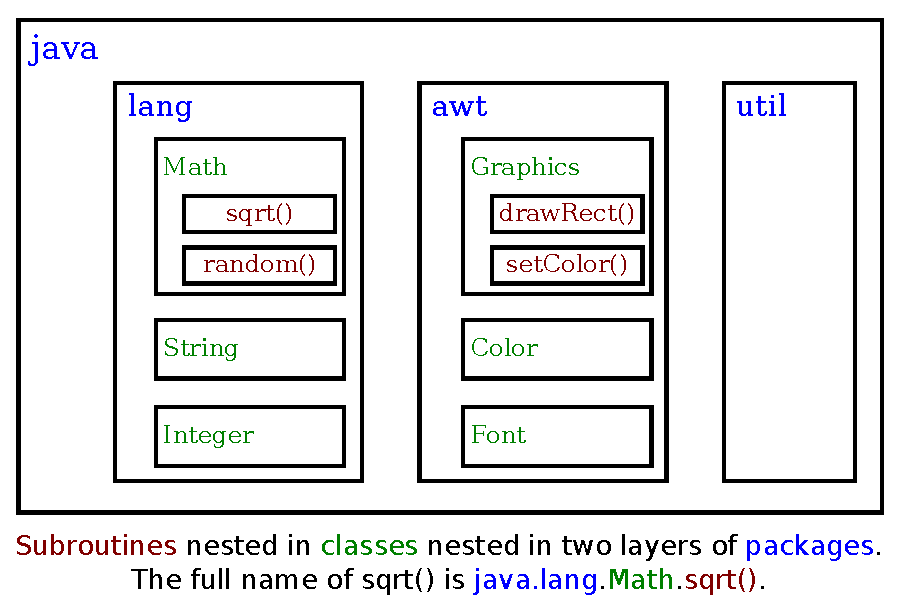
\includegraphics[scale=0.6]{images/package-class-subroutine.eps}
}

   

The official documentation for the standard Java~7 API
lists 209 different packages, including sub-packages, and
it lists 4024 classes in these packages.  Many of these are rather obscure or
very specialized, but you might want to browse through the documentation to see
what is available.  As I write this, the
documentation for the complete API can be found at
\displaycode{\weblink{http://download.oracle.com/javase/7/docs/api/}{http://download.oracle.com/javase/7/docs/api/}}\donedisplaycode

\noindent Even an expert programmer won't be familiar with the entire API,
or even a majority of it.  In this book, you'll only encounter
several dozen classes, and those will be sufficient for writing a 
wide variety of programs.


   
\subsection{Using Classes from Packages}\label{subroutines.5.3}



Let's say that you want to use the class \code{java.awt.Color} in a
program that you are writing.  Like any class, \code{java.awt.Color} is
a type, which means that you can use it to declare variables and parameters and
to specify the return type of a function. One way to do this is to use the
full name of the class as the name of the type. For example, suppose that you
want to declare a variable named \code{rectColor} of type \code{java.awt.Color}.
You could say:

\displaycode{java.awt.Color  rectColor;}\donedisplaycode


\noindent This is just an ordinary variable declaration of the form
``\bnf{type-name}~\bnf{variable-name};".
Of course, using the full name of every class can get tiresome, and you will hardly
ever see full names like \code{java.awt.Color} used in a program.
Java makes it possible to avoid using the full name of a class by \newword{importing}
the class. If you put

\displaycode{import java.awt.Color;}\donedisplaycode


\noindent at the beginning of a Java source code file, then, in the rest of the file,
you can abbreviate the full name \code{java.awt.Color} to just the simple name of
the class, which is \code{Color}.  Note that the \code{import} line comes at the start of 
a file (after the \code{package} statement, if there is one) 
and is not inside any class.  Although it is sometimes referred to
as a statement, it is more properly called an \newword{import~directive}
since it is not a statement in the usual sense.  The \code{import}
directive ``\code{import~java.awt.Color}" would allow you to say

\displaycode{Color  rectColor;}\donedisplaycode


\noindent to declare the variable.  Note that the only effect of the
\code{import} directive is to allow you to use simple class names instead of
full ``package.class" names. You aren't really importing anything substantial;
if you leave out the \code{import} directive, you can still access the class---you 
just have to use its full name.  There is a shortcut for importing all
the classes from a given package. You can import all the classes from
\code{java.awt} by saying

\displaycode{import java.awt.*;}\donedisplaycode


\noindent The ``\code{*}" is a \newword{wildcard} that matches every class in the package.
(However, it does not match sub-packages; for example, you \textbf{cannot} import the entire
contents of all the sub-packages of the \code{java} package by saying
\code{import~java.*}.)
   

Some programmers think that using a wildcard in an \code{import} statement
is bad style, since it can make a large number of class names available that you are
not going to use and might not even know about.  They think it is better to explicitly
import each individual class that you want to use.  In my own programming, I often
use wildcards to import all the classes from the most relevant packages, and use
individual imports when I am using just one or two classes from a given package.


In fact, any Java program that uses a graphical user interface is likely to
use many classes from the \code{java.awt} and \code{javax.swing} packages
as well as from another package named \code{java.awt.event}, 
and I often begin such programs with
   
\displaycode{import java.awt.*;
import java.awt.event.*;
import javax.swing.*;}\donedisplaycode

   
\noindent A program that works with networking might include the line
``\code{import java.net.*;}", while one that reads or writes files might
use ``\code{import java.io.*;}".  But when you start importing lots
of packages in this way, you have to be careful about one thing: It's possible
for two classes that are in different packages to have the same name. For
example, both the \code{java.awt} package and the \code{java.util} package
contain a class named \code{List}. If you import both \code{java.awt.*} and
\code{java.util.*}, the simple name \code{List} will be ambiguous. If you
try to declare a variable of type \code{List}, you will get a compiler error
message about an ambiguous class name.  You can still use both classes in your program: Use the full
name of the class, either \code{java.awt.List} or \code{java.util.List}.
Another solution, of course, is to use \code{import} to import the individual classes you
need, instead of importing entire packages.


Because the package \code{java.lang} is so fundamental, all the classes in
\code{java.lang} are \textbf{automatically} imported into every
program. It's as if every program began with the statement ``\code{import
java.lang.*;}". This is why we have been able to use the class name
\classname{String} instead of \code{java.lang.String}, and \code{Math.sqrt()}
instead of \code{java.lang.Math.sqrt()}. It would still, however, be
perfectly legal to use the longer forms of the names.


Programmers can create new packages. Suppose that you want some classes that
you are writing to be in a package named \code{utilities}. Then the source
code file that defines those classes must begin with the line

\displaycode{package utilities;}\donedisplaycode


\noindent This would come even before any \code{import} directive in that file.
Furthermore, the source code file
would be placed in a folder with the same name as the package, ``utilities" in this example.
And a class that is in a subpackage must be in a subfolder.  For example, a class in
a package named \code{utilities.net} would be in folder named ``net" inside a
folder named ``utilities".  A class that is
in a package automatically has access to other classes in the same package; that is,
a class doesn't have to import the package in which it is defined.
   

In projects that define large numbers of classes, it makes sense to organize
those classes into packages. It also makes sense for programmers to
create new packages as toolboxes that provide functionality and APIs for
dealing with areas not covered in the standard Java API. (And in fact such
``toolmaking" programmers often have more prestige than the applications
programmers who use their tools.)


However, with just a couple of exceptions, 
I will not be creating packages in this textbook. For the purposes of this
book, you need to know about packages mainly so that you will be able to import the standard
packages. These packages are always available to the programs that you write.
You might wonder where the standard classes are actually located.  Again, that can
depend to some extent on the version of Java that you are using, but in recent standard
versions, they are stored in \newword{jar files} in a subdirectory named \code{lib}
inside the Java Runtime Environment installation
directory.  A jar (or ``Java archive") file is a single file that can contain many classes.
Most of the standard classes can be found in a jar file named \code{rt.jar}.
In fact, Java programs are generally distributed in the form of jar files, instead of as
individual class files.


Although we won't be creating packages explicitly, \textbf{every}
class is actually part of a package. If a class is not specifically placed in a
package, then it is put in something called the \newword{default package}, 
which has no name.  Almost all the examples that you see in this book
are in the default package.

   


   
\subsection{Javadoc}\label{subroutines.5.4}

   

To use an API effectively, you need good documentation for it.  The documentation for
most Java APIs is prepared using a system called \newword{Javadoc}.  For example,
this system is used to prepare the documentation for Java's standard packages.  And almost
everyone who creates a toolbox in Java publishes Javadoc documentation for it.
   

Javadoc documentation is prepared from special comments that are placed in the Java
source code file.  Recall that one type of Java comment begins with \code{/*} and ends with~\code{*/}.
A Javadoc comment takes the same form, but it begins with \code{/**} rather than simply~\code{/*}.
You have already seen comments of this form in many of the examples in this book.
      

Note that a Javadoc comment must be placed just \textbf{before} the subroutine that
it is commenting on.  This rule is always followed.  You can have Javadoc
comments for subroutines, for member variables, and for classes.  The Javadoc
comment always immediately \textbf{precedes} the thing it is commenting on.


Like any comment, a Javadoc comment is ignored by the computer when the file is compiled.
But there is a tool called \code{javadoc} that reads Java source code files, extracts
any Javadoc comments that it finds, and creates a set of Web pages containing the comments
in a nicely formatted, interlinked form.  By default, \code{javadoc} will only collect
information about \code{public} classes, subroutines, and member variables, but
it allows the option of creating documentation for non-public things as well.  If
\code{javadoc} doesn't find any Javadoc comment for something, it will construct
one, but the comment will contain only basic information such as the name and type
of a member variable or the name, return type, and parameter list of a subroutine.
This is \textbf{syntactic} information.  To add information about semantics and pragmatics,
you have to write a Javadoc comment.
   

As an example, you can look at the documentation Web page for \classname{TextIO}.
The documentation page was created by applying the \code{javadoc} tool
to the source code file, \sourceref{TextIO.java}.  If you have downloaded the on-line
version of this book, the documentation can be found in the \code{TextIO\_Javadoc}
directory, or you can find a link to it in the on-line version of this section.


In a Javadoc comment, the \code{*}'s at the start of each line are optional.
The \code{javadoc} tool will remove them.  In addition to normal text, the comment
can contain certain special codes.  For one thing, the comment can contain
\newword{HTML mark-up} commands.  HTML is the language that is used to
create web pages, and Javadoc comments are meant to be shown on web pages.  The
\code{javadoc} tool will copy any HTML commands in the comments to the web
pages that it creates.  The book will not teach you HTML, but as 
an example, you can add \code{\<p\>} to indicate the start of
a new paragraph.  (Generally, in the absence of HTML commands, blank lines and
extra spaces in the comment are ignored.  Furthermore, the characters \& and
\< have special meaning in HTML and should not be used in Javadoc comments except
with those meanings; they can be written as \code{\&amp;} and~\code{\&lt;}.)
   

In addition to HTML commands, Javadoc comments can include \newword{doc tags},
which are processed as commands by the \code{javadoc} tool.  A doc tag has a
name that begins with the character~\code{@}.  I will only discuss four
tags:  \code{@author}, \code{@param}, \code{@return}, and \code{@throws}.
The \code{@author} tag can be used only for a class, and should be followed by the
name of the author.  The other three
tags are used in Javadoc comments for a subroutine to provide information about its
parameters, its return value, and the exceptions
that it might throw. These tags
\textbf{must} be placed at the end of the comment, after any description of the subroutine
itself.  The syntax for using them is:


\displaycode{@param  \bnf{parameter-name}   \bnf{description-of-parameter}
   
@return  \bnf{description-of-return-value}
   
@throws  \bnf{exception-class-name}   \bnf{description-of-exception}}\donedisplaycode

   
\noindent The \bnf{descriptions} can extend over several lines.  The description ends at
the next doc tag or at the end of the comment.  You can include a \code{@param} tag for
every parameter of the subroutine and a \code{@throws} for as many types of exception
as you want to document.  You should have a \code{@return} tag only for a
non-void subroutine.  These tags do not have to be given in any particular order.


Here is an example that doesn't do anything
exciting but that does use all three types of doc tag:
   
\displaycode{/**
 * This subroutine computes the area of a rectangle, given its width
 * and its height.  The length and the width should be positive numbers.
 * @param width the length of one side of the rectangle
 * @param height the length the second side of the rectangle
 * @return the area of the rectangle
 * @throws IllegalArgumentException if either the width or the height
 *    is a negative number.
 */
public static double areaOfRectangle( double length, double width ) \{
    if ( width \< 0  ||  height \< 0 )
       throw new IllegalArgumentException("Sides must have positive length.");
    double area;
    area = width * height;
    return area; 
\}}\donedisplaycode

   

I use Javadoc comments for many of my examples.  I encourage you to use
them in your own code, even if you don't plan to generate Web page documentation
of your work, since it's a standard format that other Java programmers will be
familiar with.


If you do want to create Web-page documentation, you need to run the
\code{javadoc} tool.  This tool is available as a command in the Java Development
Kit that was discussed in Section~\ref{basics.6}.  You can use \code{javadoc}
in a command line interface similarly to the way that the \code{javac} and
\code{java} commands are used.  Javadoc can also be applied in the
integrated development environments that were also discussed in 
Section~\ref{basics.6}.  I won't go into any of the details here; consult the
documentation for your programming environment.
   


   
\subsection{Static Import}\label{subroutines.5.5}



Before ending this section, I will mention an extension of the \code{import} directive.
We have seen that \code{import} makes it possible to refer to a class
such as \code{java.awt.Color} using its simple name, \classname{Color}.
But you still have to use compound names to refer to static member variables such
as \code{System.out} and to static methods such as \code{Math.sqrt}.
   

There is another form of the \code{import} directive that can
be used to import \code{static} members of a class in the same way that
the ordinary \code{import} directive imports classes from a package.
That form of the directive is called a \newword{static import},
and it has syntax
   
\displaycode{import static \bnf{package-name}.\bnf{class-name}.\bnf{static-member-name};}\donedisplaycode

   
\noindent to import one static member name from a class, or
   
\displaycode{import static \bnf{package-name}.\bnf{class-name}.*;}\donedisplaycode

   
\noindent to import all the public static members from a class.  For example, if you preface
a class definition with
   
\displaycode{import static java.lang.System.out;}\donedisplaycode

   
\noindent then you can use the simple name \code{out} instead of the compound name \code{System.out}.
This means you can say \code{out.println} instead of \code{System.out.println}.  If you
are going to work extensively with the \classname{Math} class, you can preface
your class definition with
   
\displaycode{import static java.lang.Math.*;}\donedisplaycode

   
\noindent This would allow you to say \code{sqrt} instead of \code{Math.sqrt}, \code{log}
instead of \code{Math.log}, \code{PI} instead of \code{Math.PI}, and so on.


Note that the static import directive requires a \bnf{package-name}, even for classes in
the standard package \code{java.lang}.  One consequence of this is that you can't do a 
static import from a class in the default package.  In particular, it is not possible to do
a static import from my \classname{TextIO} class---if you want to do that,
you have to move \classname{TextIO} into a package.



   



   



\section{More on Program Design}\label{subroutines.6}



\start{{\Large U}nderstanding how programs work} is one thing.
Designing a program to perform some particular task is another thing
altogether. In Section~\ref{control.2}, I discussed how pseudocode and
stepwise refinement can be used to methodically develop an algorithm. We can
now see how subroutines can fit into the process.
      

Stepwise refinement is inherently a top-down process, but the process does
have a ``bottom," that is, a point at which you stop refining the pseudocode
algorithm and translate what you have directly into proper program code.
In the absence of subroutines, the process would not bottom out until
you get down to the level of assignment statements and very primitive
input/output operations. But if you have subroutines lying around to perform
certain useful tasks, you can stop refining as soon as you've managed to
express your algorithm in terms of those tasks.


This allows you to add a bottom-up element to the top-down approach of
stepwise refinement. Given a problem, you might start by writing some
subroutines that perform tasks relevant to the problem domain. The subroutines
become a toolbox of ready-made tools that you can integrate into your algorithm
as you develop it. (Alternatively, you might be able to buy or find a software
toolbox written by someone else, containing subroutines that you can use in
your project as black boxes.)


Subroutines can also be helpful even in a strict top-down approach. As you
refine your algorithm, you are free at any point to take any sub-task in the
algorithm and make it into a subroutine. Developing that subroutine then
becomes a separate problem, which you can work on separately. Your main
algorithm will merely call the subroutine. This, of course, is just a way of
breaking your problem down into separate, smaller problems. It is still a
top-down approach because the top-down analysis of the problem tells you what
subroutines to write. In the bottom-up approach, you start by writing or
obtaining subroutines that are relevant to the problem domain, and you build
your solution to the problem on top of that foundation of subroutines.

\subsection{Preconditions and Postconditions}\label{subroutines.6.1}



When working with subroutines as building blocks, it is important to be
clear about how a subroutine interacts with the rest of the program. This
interaction is specified by the \newword{contract} of the
subroutine, as discussed in Section~\ref{subroutines.1}. A convenient
way to express the contract of a subroutine is in terms of 
\newword{preconditions} and \newword{postconditions}.


A precondition of a subroutine is something that must be true when the
subroutine is called, if the subroutine is to work correctly. For example, for
the built-in function \code{Math.sqrt(x)}, a precondition is that the
parameter, \code{x}, is greater than or equal to zero, since it is not
possible to take the square root of a negative number. In terms of a contract,
a precondition represents an obligation of the \textit{caller} of the subroutine.
If you call a subroutine without meeting its precondition, then there is no
reason to expect it to work properly. The program might crash or give incorrect
results, but you can only blame yourself, not the subroutine.


A postcondition of a subroutine represents the other side of the contract.
It is something that will be true after the subroutine has run (assuming that
its preconditions were met---and that there are no bugs in the subroutine).
The postcondition of the function \code{Math.sqrt()} is that the square of
the value that is returned by this function is equal to the parameter that is
provided when the subroutine is called. Of course, this will only be true if
the precondition---that the parameter is greater than or equal to zero---is
met. A postcondition of the built-in subroutine \code{System.out.print(x)} is
that the value of the parameter has been displayed on the screen.


Preconditions most often give restrictions on the acceptable values of
parameters, as in the example of \code{Math.sqrt(x)}. However, they can also
refer to global variables that are used in the subroutine.  Or if it only makes
sense to call the subroutine at certain times, the precondition might refer to 
the state that the program must be in when the subroutine is called.


The postcondition of a subroutine, on the other hand, 
specifies the task that it performs. For a function, the
postcondition should specify the value that the function returns.


Subroutines are sometimes described by comments that explicitly specify their
preconditions and postconditions. When you are given a pre-written subroutine,
a statement of its preconditions and postconditions tells you how to use it and
what it does. When you are assigned to write a subroutine, the preconditions
and postconditions give you an exact specification of what the subroutine is
expected to do. I will use this approach in the example that constitutes the
rest of this section. The comments are given in the form of
Javadoc comments, but I will explicitly
label the preconditions and postconditions.  (Many computer scientists think that new doc
tags \code{@precondition} and \code{@postcondition} should
be added to the Javadoc system for explicit labeling of preconditions
and postconditions, but that has not yet been done.)



\subsection{A Design Example}\label{subroutines.6.2}



Let's work through an example of program design using subroutines. In this
example, we will use pre-written subroutines as building blocks and we will also design
new subroutines that we need to complete the project.  The API that I will use here
is defined in \sourceref{Mosaic.java}, which in turns depends on
\sourceref{MosaicPanel.java}.  To compile and run a program that uses the
API, the classes \classname{Mosaic} and \classname{MosaicPanel}
must be available.  That is, the files \code{Mosaic.java} and
\code{MosaicPanel.java}, or the the corresponding compiled class files,
must be in the same folder as the class that defines the program.


So, suppose that I have found an already-written class called \code{Mosaic}.
This class allows a program to work with a window that displays little colored
rectangles arranged in rows and columns. The window can be opened, closed, and
otherwise manipulated with static member subroutines defined in the
\code{Mosaic} class.  In fact, the class defines a toolbox or API
that can be used for working with such windows.  Here are some of the
available routines in the API, with Javadoc-style comments. (Remeber that
a Javadoc comment comes before the thing that it is commenting on.)
   
\displaycode{/**
 * Opens a "mosaic" window on the screen.
 *
 * Precondition:   The parameters rows, cols, w, and h are positive integers.
 * Postcondition:  A window is open on the screen that can display rows and
 *                   columns of colored rectangles.  Each rectangle is w pixels
 *                   wide and h pixels high.  The number of rows is given by
 *                   the first parameter and the number of columns by the
 *                   second.  Initially, all rectangles are black.
 *
 * Note:  The rows are numbered from 0 to rows - 1, and the columns are 
 * numbered from 0 to cols - 1.
 */
\newcode{public static void open(int rows, int cols, int w, int h)}
   
   
/**
 * Sets the color of one of the rectangles in the window.
 *
 * Precondition:   row and col are in the valid range of row and column numbers,
 *                   and r, g, and b are in the range 0 to 255, inclusive.
 * Postcondition:  The color of the rectangle in row number row and column
 *                   number col has been set to the color specified by r, g,
 *                   and b.  r gives the amount of red in the color with 0 
 *                   representing no red and 255 representing the maximum 
 *                   possible amount of red.  The larger the value of r, the 
 *                   more red in the color.  g and b work similarly for the 
 *                   green and blue color components.
 */
\newcode{public static void setColor(int row, int col, int r, int g, int b)}

   
/**
 * Gets the red component of the color of one of the rectangles.
 *
 * Precondition:   row and col are in the valid range of row and column numbers.
 * Postcondition:  The red component of the color of the specified rectangle is
 *                   returned as an integer in the range 0 to 255 inclusive.
 */
\newcode{public static int getRed(int row, int col)}

   
/**
 * Like getRed, but returns the green component of the color.
 */
\newcode{public static int getGreen(int row, int col)}

   
/**
 * Like getRed, but returns the blue component of the color.
 */
\newcode{public static int getBlue(int row, int col)}

   
/**
 * Tests whether the mosaic window is currently open.
 *
 * Precondition:   None.
 * Postcondition:  The return value is true if the window is open when this
 *                   function is called, and it is false if the window is
 *                   closed.
 */
\newcode{public static boolean isOpen()}

   
/**
 * Inserts a delay in the program (to regulate the speed at which the colors
 * are changed, for example).
 *
 * Precondition:   milliseconds is a positive integer.
 * Postcondition:  The program has paused for at least the specified number
 *                   of milliseconds, where one second is equal to 1000
 *                   milliseconds.
 */
\newcode{public static void delay(int milliseconds)}}\donedisplaycode

   

Remember that these subroutines are members of the \code{Mosaic}
class, so when they are called from outside \code{Mosaic}, the name of the class
must be included as part of the name of the routine.  For example,
we'll have to use the name \code{Mosaic.isOpen()} rather than simply
\code{isOpen()}.


You'll notice that the comments on the subroutine don't specify what
happens when the preconditions are \textbf{not} met.  Although a subroutine
is not really obligated by its contract to do anything particular in that
case, it would be good to know what happens.  For example, if the
precondition, ``row and col are in the valid range of row and column numbers,"
on the \code{setColor()} or \code{getRed()} routine is violated,
an \classname{IllegalArgumentException} will be thrown.
Knowing that fact would allow you to write programs that catch and handle
the exception, and it would be good to document it with a \code{@throws}
doc tag in the Javadoc comment.
Other questions remain about the behavior of the subroutines.
For example, what happens if you call \code{Mosaic.open()} and there
is already a mosaic window open on the screen?  (In fact, the old one will
be closed, and a new one will be created.)  It's difficult to fully document
the behavior of a piece of software---sometimes, you just have to 
experiment or look at the full source code.


\mybreak



My idea for a program is to use the \code{Mosaic} class as the basis for a neat
animation. I want to fill the window with randomly colored squares, and then
randomly change the colors in a loop that continues as long as the window is
open. ``Randomly change the colors" could mean a lot of different things, but
after thinking for a while, I decide it would be interesting to have a
``disturbance" that wanders randomly around the window, changing the color of
each square that it encounters. Here's a picture showing what the contents of the window
might look like at one point in time:


\par\dumpfigure{
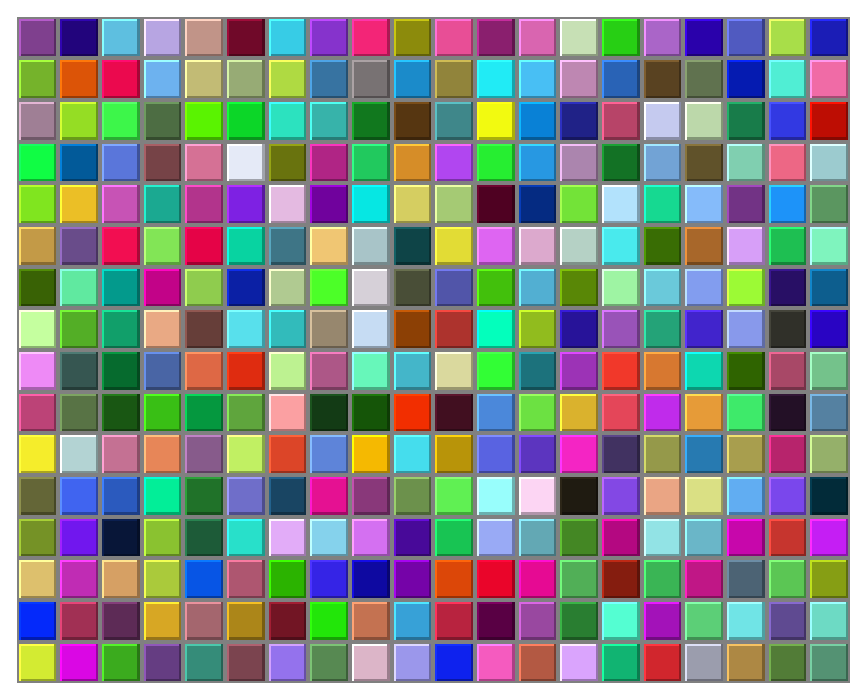
\includegraphics[scale=0.5]{images/mosaic.eps}
}




With basic routines for manipulating the window as a foundation, I can turn
to the specific problem at hand. A basic outline for my program is

\displaycode{Open a Mosaic window
Fill window with random colors
Move around, changing squares at random}\donedisplaycode


\noindent Filling the window with random colors seems like a nice coherent task that I
can work on separately, so let's decide to write a separate subroutine to do
it. The third step can be expanded a bit more, into the steps: Start in the
middle of the window, then keep moving to new squares and changing the color
of those squares. This should continue as long as the mosaic window is still
open. Thus we can refine the algorithm to:

\displaycode{Open a Mosaic window
Fill window with random colors
Set the current position to the middle square in the window
As long as the mosaic window is open:
   Randomly change color of the square at the current position
   Move current position up, down, left, or right, at random}\donedisplaycode


\noindent I need to represent the current position in some way. That can be done with
two \ptype{int} variables named \code{currentRow} and
\code{currentColumn} that hold the row number and the column number of 
the square where the disturbance is currently located.  I'll use 16 rows and 20 columns of squares in my
mosaic, so setting the current position to be in the center means setting
\code{currentRow} to 8 and \code{currentColumn} to 10. I already have a
subroutine, \code{Mosaic.open()}, to open the window, and I have a function,
\code{Mosaic.isOpen()}, to test whether the window is open. To keep the main
routine simple, I decide that I will write two more subroutines of my own to
carry out the two tasks in the while loop. The algorithm can then be written in
Java as:

\displaycode{Mosaic.open(16,20,25,25)
fillWithRandomColors();
currentRow = 8;       // Middle row, halfway down the window.
currentColumn = 10;   // Middle column.
while ( Mosaic.isOpen() ) \{
    changeToRandomColor(currentRow, currentColumn);
    randomMove();      
\}}\donedisplaycode


\noindent With the proper wrapper, this is essentially the \code{main()} routine of
my program. It turns out I have to make one small modification: To prevent the
animation from running much, much too fast, the line ``\code{Mosaic.delay(1);}" is added
to the \code{while} loop.


The \code{main()} routine is taken care of, but to complete the program, I
still have to write the subroutines \code{fillWithRandomColors()},
\code{changeToRandomColor(int,int)}, and \code{randomMove()}. Writing each
of these subroutines is a separate, small task. The
\code{fillWithRandomColors()} routine is defined by the postcondition that
``each of the rectangles in the mosaic has been changed to a random color."
Pseudocode for an algorithm to accomplish this task can be given as:

\displaycode{For each row:
   For each column:
      set the square in that row and column to a random color}\donedisplaycode


\noindent ``For each row" and ``for each column" can be implemented as for loops. We've
already planned to write a subroutine \code{changeToRandomColor} that can be
used to set the color. (The possibility of reusing subroutines in several
places is one of the big payoffs of using them!) So,
\code{fillWithRandomColors()} can be written in proper Java as:

\displaycode{static void fillWithRandomColors() \{
   for (int row = 0; row \< 16; row++)
      for (int column = 0; column \< 20; column++)
         changeToRandomColor(row,column);
\}}\donedisplaycode



Turning to the \code{changeToRandomColor} subroutine, we already have a
method in the \code{Mosaic} class, \code{Mosaic.setColor()}, 
that can be used to change the
color of a square. If we want a random color, we just have to choose random
values for \code{r}, \code{g}, and \code{b}. According to the
precondition of the \code{Mosaic.setColor()} subroutine, these random values
must be integers in the range from 0 to 255. A formula for randomly selecting
such an integer is ``\code{(int)(256*Math.random())}". So the random color
subroutine becomes:

\displaycode{static void changeToRandomColor(int rowNum, int colNum) \{
     int red = (int)(256*Math.random());
     int green = (int)(256*Math.random());  
     int blue = (int)(256*Math.random());
     Mosaic.setColor(rowNum,colNum,red,green,blue);  
\}}\donedisplaycode



Finally, consider the \code{randomMove} subroutine, which is supposed to
randomly move the disturbance up, down, left, or right. To make a random choice
among four directions, we can choose a random integer in the range 0 to 3. If
the integer is 0, move in one direction; if it is 1, move in another direction;
and so on. The position of the disturbance is given by the variables
\code{currentRow} and \code{currentColumn}. To ``move up" means to subtract
1 from \code{currentRow}. This leaves open the question of what to do if
\code{currentRow} becomes -1, which would put the disturbance above the
window (which would violate a precondition of several of the \classname{Mosaic}
subroutines).
Rather than let this happen, I decide to move the disturbance to the
opposite edge of the grid by setting \code{currentRow} to 15. (Remember that
the 16 rows are numbered from 0 to 15.)  An alternative to jumping to the opposite
edge would be to simply do nothing in this case.  Moving the disturbance down, left, or
right is handled similarly. If we use a \code{switch} statement to decide
which direction to move, the code for \code{randomMove} becomes:

\displaycode{int directionNum;
directionNum = (int)(4*Math.random());
switch (directionNum) \{
   case 0:  // move up 
      currentRow--;
      if (currentRow \< 0)   // CurrentRow is outside the mosaic;
         currentRow = 15;   // move it to the opposite edge.
      break;
   case 1:  // move right
      currentColumn++;
      if (currentColumn \>= 20)
         currentColumn = 0;
      break; 
   case 2:  // move down
      currentRow++;
      if (currentRow \>= 16)
         currentRow = 0;
      break;
   case 3:  // move left
      currentColumn--;
      if (currentColumn \< 0)
         currentColumn = 19;
      break; 
\}}\donedisplaycode

   

   
\subsection{The Program}\label{subroutines.6.3}



Putting this all together, we get the following complete program.  Note that I've added Javadoc-style
comments for the class itself and for each of the subroutines. The
variables \code{currentRow} and \code{currentColumn} are defined as static
members of the class, rather than local variables, because each of them is used
in several different subroutines.  You can find a copy of the source code in
\sourceref{RandomMosaicWalk.java}.  Remember that this program actually 
depends on two other files, \sourceref{Mosaic.java} and \sourceref{MosaicPanel.java}.

\displaycode{/**
 * This program opens a window full of randomly colored squares.  A "disturbance"
 * moves randomly around in the window, randomly changing the color of each
 * square that it visits.  The program runs until the user closes the window.
 */
public class RandomMosaicWalk \{

    static int currentRow;    // Row currently containing the disturbance.
    static int currentColumn; // Column currently containing disturbance.

    /**
     * The main program creates the window, fills it with random colors,
     * and then moves the disturbance in a random walk around the window
     * as long as the window is open.
     */
    public static void main(String[] args) \{
        Mosaic.open(16,20,25,25);
        fillWithRandomColors();
        currentRow = 8;   // start at center of window
        currentColumn = 10;
        while (Mosaic.isOpen()) \{
            changeToRandomColor(currentRow, currentColumn);
            randomMove();
            Mosaic.delay(1);
        \}
    \}  // end main

    /**
     * Fills the window with randomly colored squares.
     * Precondition:   The mosaic window is open.
     * Postcondition:  Each square has been set to a random color. 
     */
    static void fillWithRandomColors() \{
        for (int row=0; row \< 16; row++) \{
            for (int column=0; column \< 20; column++) \{
                changeToRandomColor(row, column);  
            \}
        \}
    \}  // end fillWithRandomColors

    /**
     * Changes one square to a new randomly selected color.
     * Precondition:   The specified rowNum and colNum are in the valid range
     *                 of row and column numbers.
     * Postcondition:  The square in the specified row and column has
     *                 been set to a random color.
     * @param rowNum the row number of the square, counting rows down
     *      from 0 at the top
     * @param colNum the column number of the square, counting columns over
     *      from 0 at the left
     */
    static void changeToRandomColor(int rowNum, int colNum) \{
        int red = (int)(256*Math.random());    // Choose random levels in range
        int green = (int)(256*Math.random());  //     0 to 255 for red, green, 
        int blue = (int)(256*Math.random());   //     and blue color components.
        Mosaic.setColor(rowNum,colNum,red,green,blue);  
    \}  // end changeToRandomColor

    /**
     * Move the disturbance.
     * Precondition:   The global variables currentRow and currentColumn
     *                 are within the legal range of row and column numbers.
     * Postcondition:  currentRow or currentColumn is changed to one of the
     *                 neighboring positions in the grid -- up, down, left, or
     *                 right from the current position.  If this moves the
     *                 position outside of the grid, then it is moved to the
     *                 opposite edge of the grid.
     */
    static void randomMove() \{
        int directionNum; // Randomly set to 0, 1, 2, or 3 to choose direction.
        directionNum = (int)(4*Math.random());
        switch (directionNum) \{
        case 0:  // move up 
            currentRow--;
            if (currentRow \< 0)
                currentRow = 15;
            break;
        case 1:  // move right
            currentColumn++;
            if (currentColumn \>= 20)
                currentColumn = 0;
            break; 
        case 2:  // move down
            currentRow ++;
            if (currentRow \>= 16)
                currentRow = 0;
            break;
        case 3:  // move left  
            currentColumn--;
            if (currentColumn \< 0)
                currentColumn = 19;
            break; 
        \}
    \}  // end randomMove

\} // end class RandomMosaicWalk}\donedisplaycode





   



\section{The Truth About Declarations}\label{subroutines.7}



\start{{\Large N}ames are fundamental to programming}, as I said a
few chapters ago. There are a lot of details involved in declaring and using
names. I have been avoiding some of those details. In this section, I'll reveal
most of the truth (although still not the full truth) about declaring and using
variables in Java. The material in the subsections ``Initialization
in Declarations" and ``Named Constants" is
particularly important, since I will be using it regularly from now on.

\subsection{Initialization in Declarations}\label{subroutines.7.1}



When a variable declaration is executed, memory is allocated for the
variable. This memory must be initialized to contain some definite value before
the variable can be used in an expression. In the case of a local variable, the
declaration is often followed closely by an assignment statement that does the
initialization. For example,

\displaycode{int count;    // Declare a variable named count.
count = 0;    // Give count its initial value.}\donedisplaycode



However, the truth about declaration statements is that it is legal to
include the initialization of the variable in the declaration statement. The
two statements above can therefore be abbreviated as

\displaycode{int count = 0;  // Declare count and give it an initial value.}\donedisplaycode


\noindent The computer still executes this statement in two steps: Declare the
variable \code{count}, then assign the value 0 to the newly created variable.
The initial value does not have to be a constant.  It can be any expression. It
is legal to initialize several variables in one declaration statement. For
example,

\displaycode{char firstInitial = 'D', secondInitial = 'E';
                
int x, y = 1;   // OK, but only y has been initialized!
  
int N = 3, M = N+2;  // OK, N is initialized 
                     //        before its value is used.}\donedisplaycode


\noindent This feature is especially common in \code{for} loops, since it makes it
possible to declare a loop control variable at the same point in the loop where
it is initialized.  Since the loop control variable generally has nothing to do
with the rest of the program outside the loop, it's reasonable to have its
declaration in the part of the program where it's actually used. For
example:

\displaycode{for ( \newcode{int i = 0};  i \< 10;  i++ ) \{
   System.out.println(i);
\}}\donedisplaycode


\noindent You should remember that this is simply an abbreviation for the
following, where I've added an extra pair of braces to show that \code{i} is
considered to be local to the \code{for} statement and no longer exists after
the \code{for} loop ends:

\displaycode{\{
   int i;
   for ( i = 0;  i \< 10;  i++ ) \{
      System.out.println(i);
   \}
\}}\donedisplaycode

   


A member variable can also be initialized at the point where it is declared, just as
for a local variable.  For example:

\displaycode{public class Bank \{
   private static double interestRate = 0.05;
   private static int maxWithdrawal = 200;
     .
     .  // More variables and subroutines.
     .
\}}\donedisplaycode


\noindent A static member variable is created as soon as the class is loaded by the
Java interpreter, and the initialization is also done at that time. In the case
of member variables, this is not simply an abbreviation for a declaration
followed by an assignment statement. Declaration statements are the only type
of statement that can occur outside of a subroutine. Assignment statements
cannot, so the following is illegal:

\displaycode{public class Bank \{
   private static double interestRate;
   interestRate = 0.05;  // \newcode{ILLEGAL:}
   .                     //    \newcode{Can't be outside a subroutine!}:
   .
   .}\donedisplaycode



Because of this, declarations of member variables often include initial
values.  In fact, as mentioned in Subsection~\ref{subroutines.2.4}, if no initial value is
provided for a member variable, then a default initial value is used. For
example, when declaring an integer member variable, \code{count},
``\code{static int count;}" is equivalent to ``\code{static~int count~=~0;}".


Even array variables can be initialized.  An array contains several elements, not
just a single value.  To initialize an array variable, you can provide a list of
values, separated by commas, and enclosed between a pair of braces.  For example:

\displaycode{int[] smallPrimes = \{ 2, 3, 5, 7, 11, 13, 17, 23, 29 \};}\donedisplaycode


\noindent In this statement, an array of \ptype{int} of length 9 is created
and filled with the values in the list.  The length of the array is determined
by the number of items in the list.


Note that this syntax for initializing arrays \textbf{cannot} be used in assignment
statements.  It can only be used in a declaration statement at the time when the
array variable is declared.


It is also possible to initialize an array variable with an array created using
the \code{new} operator (which \textbf{can} also be used in assignment 
statements).  For example:

\displaycode{String[] namelist = new String[100];}\donedisplaycode


\noindent but in that case, of course, all the array elements will have their default value.




\subsection{Named Constants}\label{subroutines.7.2}



Sometimes, the value of a variable is not supposed to change after it is
initialized. For example, in the above example where \code{interestRate} is
initialized to the value \code{0.05}, it's quite possible that 0.05 is meant to be the
value throughout the entire program. In that case, the programmer is probably
defining the variable, \code{interestRate}, to give a meaningful name to the
otherwise meaningless number, \code{0.05}. It's easier to understand what's going on
when a program says ``\code{principal += principal*interestRate;}" rather than
``\code{principal += principal*0.05;}".


In Java, the modifier ``\code{final}" can be applied to a variable
declaration to ensure that the value stored in the variable cannot be changed after
the variable has been initialized. For example, if the member variable
\code{interestRate} is declared with

\displaycode{public \newcode{final} static double interestRate = 0.05;}\donedisplaycode


\noindent then it would be impossible for the value of \code{interestRate} to change anywhere
else in the program. Any assignment statement that tries to assign a value to
\code{interestRate} will be rejected by the computer as a syntax error when
the program is compiled.  (A ``final" modifier on a public interest rate makes a lot
of sense---a bank might want to publish its interest rate, but it certainly 
wouldn't want to let random people make changes to it!)


It is legal to apply the \code{final} modifier to local variables and even
to formal parameters, but it is most useful for member variables. I will often
refer to a static member variable that is declared to be \code{final} as a
\newword{named constant}, since its value remains constant
for the whole time that the program is running. The readability of a program
can be greatly enhanced by using named constants to give meaningful names to
important quantities in the program. A recommended style rule for named
constants is to give them names that consist entirely of upper case letters,
with underscore characters to separate words if necessary. For example, the
preferred style for the interest rate constant would be

\displaycode{public final static double INTEREST\_RATE = 0.05;}\donedisplaycode


\noindent This is the style that is generally used in Java's standard classes, which
define many named constants. For example, we have already seen that the 
\classname{Math} class contains a variable \code{Math.PI}.  This variable
is declared in the \classname{Math} class as a ``public final static" variable
of type \ptype{double}.  Similarly, the \code{Color} class
contains named constants such as \code{Color.RED} and \code{Color.YELLOW}
which are public final static variables of type \code{Color}.
Many named constants are created just to give meaningful names to be used as parameters
in subroutine calls. For example, the
standard class named \code{Font} contains named constants
\code{Font.PLAIN}, \code{Font.BOLD}, and \code{Font.ITALIC}. These
constants are used for specifying different styles of text when calling various
subroutines in the \code{Font} class.
   

Enumerated type constants (see Subsection~\ref{basics.3.3}) are also examples of named
constants.  The enumerated type definition
   
\displaycode{enum Alignment \{ LEFT, RIGHT, CENTER \}}\donedisplaycode

   
\noindent defines the constants \code{Alignment.LEFT}, \code{Alignment.RIGHT},
and \code{Alignment.CENTER}.  Technically, \classname{Alignment} is
a class, and the three constants are public final static members of that class.  Defining the
enumerated type is similar to defining three constants of type, say, \ptype{int}:

   
\displaycode{public static final int ALIGNMENT\_LEFT = 0;
public static final int ALIGNMNENT\_RIGHT = 1;
public static final int ALIGNMENT\_CENTER = 2;}\donedisplaycode

   
\noindent In fact, this is how things were generally done before the introduction of enumerated
types, and it is what is done with the constants \code{Font.PLAIN}, \code{Font.BOLD}, 
and \code{Font.ITALIC} mentioned above.
Using the integer constants, you could define a variable  of type
\ptype{int} and assign it the values \code{ALIGNMENT\_LEFT},
\code{ALIGNMENT\_RIGHT}, or \code{ALIGNMENT\_CENTER} to represent different
types of alignment.  The only problem with this is that the computer has no way of
knowing that you intend the value of the variable to represent an alignment, and it
will not raise any objection if the value that is assigned to the variable is not
one of the three valid alignment values.
With the enumerated type, on the other hand, the only values
that can be assigned to a variable of type \classname{Alignment} are
the constant values that are listed in the definition of the enumerated type.  
Any attempt to assign an invalid value to the variable is a syntax error which
the computer will detect when the program is compiled.  This extra
safety is one of the major advantages of enumerated types. 
   

\mybreak



Curiously enough, one of the major reasons to use named constants is that
it's easy to change the value of a named constant. Of course, the value can't
change while the program is running. But between runs of the program, it's easy
to change the value in the source code and recompile the program. Consider the
interest rate example. It's quite possible that the value of the interest rate
is used many times throughout the program. Suppose that the bank changes the
interest rate and the program has to be modified. If the literal number 0.05
were used throughout the program, the programmer would have to track down each
place where the interest rate is used in the program and change the rate to the
new value. (This is made even harder by the fact that the number 0.05 might
occur in the program with other meanings besides the interest rate, as well as
by the fact that someone might have, say, used 0.025 to represent half the interest
rate.) On the other hand, if the named constant \code{INTEREST\_RATE} is
declared and used consistently throughout the program, then only the single
line where the constant is initialized needs to be changed.


As an extended example, I will give a new version of the
\code{RandomMosaicWalk} program from the previous
section. This version uses named constants to represent the number of rows
in the mosaic, the number of columns, and the size of each little square. The
three constants are declared as \code{final} \code{static} member variables
with the lines:

\displaycode{final static int ROWS = 20;        // Number of rows in mosaic.
final static int COLUMNS = 30;     // Number of columns in mosaic.
final static int SQUARE\_SIZE = 15; // Size of each square in mosaic.}\donedisplaycode



The rest of the program is carefully modified to use the named constants.
For example, in the new version of the program, the Mosaic window is opened
with the statement

\displaycode{Mosaic.open(ROWS, COLUMNS, SQUARE\_SIZE, SQUARE\_SIZE);}\donedisplaycode


\noindent Sometimes, it's not easy to find all the places where a named constant
needs to be used. If you don't use the named constant consistently, you've
more or less defeated the purpose.  It's always a good idea to run a program using several
different values for any named constant, to test that it works properly in all
cases.


Here is the complete new program, \code{RandomMosaicWalk2}, with all
modifications from the previous version shown in italic.
I've left out some of the comments to save space.


\displaycode{public class RandomMosaicWalk2 \{

    \newcode{final static int ROWS = 20;        // Number of rows in mosaic.
    final static int COLUMNS = 30;     // Number of columns in mosaic.
    final static int SQUARE\_SIZE = 15; // Size of each square in mosaic.}

    static int currentRow;    // Row currently containing the disturbance.
    static int currentColumn; // Column currently containing the disturbance.
 
    public static void main(String[] args) \{
        \newcode{Mosaic.open( ROWS, COLUMNS, SQUARE\_SIZE, SQUARE\_SIZE )};
        fillWithRandomColors();
        \newcode{currentRow = ROWS / 2};   // start at center of window
        \newcode{currentColumn = COLUMNS / 2};
        while (Mosaic.isOpen()) \{
            changeToRandomColor(currentRow, currentColumn);
            randomMove();
            Mosaic.delay(1);
        \}
    \}  // end main

    static void fillWithRandomColors() \{
         for (\newcode{int row=0; row \< ROWS; row++}) \{
            for (\newcode{int column=0; column \< COLUMNS; column++}) \{
                changeToRandomColor(row, column);  
            \}
         \}
    \}  // end fillWithRandomColors
 
    static void changeToRandomColor(int rowNum, int colNum) \{
         int red = (int)(256*Math.random());    // Choose random levels in range
         int green = (int)(256*Math.random());  //     0 to 255 for red, green, 
         int blue = (int)(256*Math.random());   //     and blue color components.
         Mosaic.setColor(rowNum,colNum,red,green,blue);  
     \}  // end changeToRandomColor
 
     static void randomMove() \{
         int directionNum; // Randomly set to 0, 1, 2, or 3 to choose direction.
         directionNum = (int)(4*Math.random());
         switch (directionNum) \{
            case 0:  // move up 
               currentRow--;
               if (currentRow \< 0)
                  \newcode{currentRow = ROWS - 1;}
               break;
            case 1:  // move right
               currentColumn++;
               if (\newcode{currentColumn \>= COLUMNS})
                  currentColumn = 0;
               break; 
            case 2:  // move down
               currentRow++;
               if (\newcode{currentRow \>= ROWS})
                  currentRow = 0;
               break;
            case 3:  // move left  
               currentColumn--;
               if (currentColumn \< 0)
                  \newcode{currentColumn = COLUMNS - 1};
               break; 
         \}
     \}  // end randomMove
 
\} // end class RandomMosaicWalk2}\donedisplaycode



   
\subsection{Naming and Scope Rules}\label{subroutines.7.3}



When a variable declaration is executed, memory is allocated for that
variable. The variable name can be used in at least some part of the program
source code to refer to that memory or to the data that is stored in the
memory. The portion of the program source code where the variable is valid
is called the \newword{scope} of the variable. Similarly, we
can refer to the scope of subroutine names and formal parameter names.


For static member subroutines, scope is straightforward. The scope of a
static subroutine is the entire source code of the class in which it is
defined. That is, it is possible to call the subroutine from any point in the
class, including at a point in the source code before the point where the definition
of the subroutine appears. It is even possible to call a subroutine from within itself. This is an
example of something called ``recursion," a fairly advanced topic that we will
return to in Chapter~\ref{recursion}.  If the subroutine is not \code{private},
it can also be accessed from outside the class where it is defined, using its full name.


For a variable that is declared as a static member variable in a class, the
situation is similar, but with one complication. It is legal to have a local
variable or a formal parameter that has the same name as a member variable. In
that case, within the scope of the local variable or parameter, the member
variable is \newword{hidden}. Consider, for example, a class
named \code{Game} that has the form:

\displaycode{public class Game \{

    static int count;  // member variable
 
    static void playGame() \{
        int count;  // local variable
          .
          .   // Some statements to define playGame()
          .
    \}
    
    .
    .   // More variables and subroutines.
    .
 
\}  // end Game}\donedisplaycode



In the statements that make up the body of the \code{playGame()}
subroutine, the name ``\code{count}" refers to the local variable. In the rest
of the \code{Game} class, ``\code{count}" refers to the member variable
(unless hidden by other local variables or parameters named \code{count}).
However, the member variable named
\code{count} can also be referred to by the full name \code{Game.count}.
Usually, the full name is only used outside the class where \code{count} is
defined. However, there is no rule against using it inside the class. The full
name, \code{Game.count}, can be used inside the \code{playGame()}
subroutine to refer to the member variable instead of the local variable. 
So, the full scope rule 
is that the scope of a static member variable includes the entire
class in which it is defined, but where the simple name of the member variable
is hidden by a local variable or formal parameter name, the member variable
must be referred to by its full name of the form \bnf{className}.\bnf{variableName}. 
(Scope rules for non-static members
are similar to those for static members, except that, as we shall see,
non-static members cannot be used in static subroutines.)


The scope of a formal parameter of a subroutine is the block that makes up
the body of the subroutine. The scope of a local variable extends from the
declaration statement that defines the variable to the end of the block in
which the declaration occurs. As noted above, it is possible to declare a loop
control variable of a \code{for} loop in the \code{for} statement, as in
``\code{for (int i=0; i \< 10; i++)}". The scope of such a declaration is
considered as a special case: It is valid only within the \code{for}
statement and does not extend to the remainder of the block that contains the
\code{for} statement.


It is not legal to redefine the name of a formal parameter or local variable
within its scope, even in a nested block. For example, this is not allowed:

\displaycode{void  badSub(int y) \{
    int x;
    while (y \> 0) \{
       int x;  // \newcode{ERROR:  x is already defined.}
         .
         .
         .
    \}
 \}}\donedisplaycode


\noindent In many languages, this would be legal; the declaration of \code{x} in the
\code{while} loop would hide the original declaration.  It is not legal in
Java; however, once the block in which a variable is declared ends, its name
does become available for reuse in Java. For example:

\displaycode{void goodSub(int y) \{
   while (y \> 10) \{
      int x;
        .
        .
        .
      // The scope of x ends here.
   \}
   while (y \> 0) \{
      int x;  // OK: Previous declaration of x has expired.
       .
       .
       .
   \}
\}}\donedisplaycode



You might wonder whether local variable names can hide subroutine names.
This can't happen, for a reason that might be surprising. There is no rule that
variables and subroutines have to have different names. The computer can always
tell whether a name refers to a variable or to a subroutine, because a
subroutine name is always followed by a left parenthesis. It's perfectly legal
to have a variable called \code{count} and a subroutine called \code{count}
in the same class. (This is one reason why I often write subroutine names with
parentheses, as when I talk about the \code{main()} routine. It's a good idea
to think of the parentheses as part of the name.) Even more is true: It's legal
to reuse class names to name variables and subroutines. The syntax rules of
Java guarantee that the computer can always tell when a name is being used as a
class name. A class name is a type, and so it can be used to declare variables and formal parameters
and to specify the return type of a function. This means that you could legally
have a class called \code{Insanity} in which you declare a function

\displaycode{static  Insanity  Insanity( Insanity Insanity ) \{ ... \}}\donedisplaycode



The first \code{Insanity} is the return type of the function. The second
is the function name, the third is the type of the formal parameter, and the
fourth is the name of the formal parameter. However, please remember that not everything
that is possible is a good idea!
   





   



\begin{exercises}

\exercise 
To ``capitalize" a string
means to change the first letter of each word in the string to upper case (if
it is not already upper case). For example, a capitalized version of ``Now is
the time to act!" is ``Now Is The Time To Act!". Write a subroutine named
\code{printCapitalized} that will print a capitalized version of a string to
standard output. The string to be printed should be a parameter to the
subroutine. Test your subroutine with a \code{main()} routine that gets a
line of input from the user and applies the subroutine to it.

Note that a letter is the first letter of a word if it is not immediately
preceded in the string by another letter. Recall from Exercise~3.4 that there is a standard
\ptype{boolean}-valued function \code{Character.isLetter(char)} that can be
used to test whether its parameter is a letter. There is another standard
\ptype{char}-valued function, \code{Character.toUpperCase(char)}, that
returns a capitalized version of the single character passed to it as a
parameter. That is, if the parameter is a letter, it returns the upper-case
version. If the parameter is not a letter, it just returns a copy of the
parameter.
\exercise 
The hexadecimal digits are
the ordinary, base-10 digits '0' through '9' plus the letters 'A' through 'F'.
In the hexadecimal system, these digits represent the values 0 through 15,
respectively. Write a function named \code{hexValue} that uses a
\code{switch} statement to find the hexadecimal value of a given character.
The character is a parameter to the function, and its hexadecimal value is the
return value of the function. You should count lower case letters 'a' through
'f' as having the same value as the corresponding upper case letters. If the
parameter is not one of the legal hexadecimal digits, return \code{-1} as the value of
the function.


A hexadecimal integer is a sequence of hexadecimal digits, such as 34A7,
ff8, 174204, or FADE. If \code{str} is a string containing a hexadecimal
integer, then the corresponding base-10 integer can be computed as follows:

\displaycode{value = 0;
for ( i = 0; i \< str.length();  i++ )
   value = value*16 + hexValue( str.charAt(i) );}\donedisplaycode


\noindent Of course, this is not valid if \code{str} contains any characters that
are not hexadecimal digits. Write a program that reads a string from the user.
If all the characters in the string are hexadecimal digits, print out the
corresponding base-10 value. If not, print out an error message.

\exercise 
Write a function that
simulates rolling a pair of dice until the total on the dice comes up to be a
given number. The number that you are rolling for is a parameter to the
function. The number of times you have to roll the dice is the return value of
the function. The parameter should be one of the possible totals:
2, 3, \dots, 12.  The function should throw an \classname{IllegalArgumentException}
if this is not the case.  Use your function in a program that computes and prints the
number of rolls it takes to get snake eyes. (Snake eyes means that the total
showing on the dice is 2.)
\exercise 
This exercise builds on Exercise~4.3.
Every time you roll the dice repeatedly, trying to get a given
total, the number of rolls it takes can be different. The question naturally
arises, what's the average number of rolls to get a given total? Write a function that performs the
experiment of rolling to get a given total 10000 times. The desired total is a
parameter to the subroutine. The average number of rolls is the return value.
Each individual experiment should be done by calling the function you wrote for
Exercise~4.3. Now, write a main program that will call your function once for
each of the possible totals (2, 3, ..., 12). It should make a table of the
results, something like:

\displaycode{Total On Dice     Average Number of Rolls
-------------     -----------------------
       2               35.8382
       3               18.0607
       .                .
       .                .}\donedisplaycode


\exercise 
The sample program
\sourceref{RandomMosaicWalk.java} from
Section~\ref{subroutines.6} shows a ``disturbance" that wanders around a
grid of colored squares. When the disturbance visits a square, the color of
that square is changed.  Here's an idea for a variation on that program.
In the new version, all the squares start
out with the default color, black. Every time the disturbance visits a square,
a small amount is added to the green component of the color of that square.
The result will be a visually interesting effect, as the path followed by the
disturbance gradually turns a brighter and brighter green.

Write a subroutine that will add 25 to the green component of one of the squares in the
mosaic.  (But don't let the green component go over 255, since that's the largest
legal value for a color component.)
The row and column numbers of the square should be given as parameters
to the subroutine. Recall that you can discover the current green component of
the square in row \code{r} and column \code{c} with the function call
\code{Mosaic.getGreen(r,c)}. Use your subroutine as a substitute for the
\code{changeToRandomColor()} subroutine in the program \sourceref{RandomMosaicWalk2.java}.
(This is the improved version of the program from Section~\ref{subroutines.7} that uses named constants for
the number of rows, number of columns, and square size.) Set the number of rows
and the number of columns to 80. Set the square size to 5.

By default, the rectangles in the mosaic have a ``3D" appearance and a gray border that makes
them look nicer in the random walk program.  But for this program, you want to turn off that
effect.  To do so, call \code{Mosaic.setUse3DEffect(false)} in the main program.

Don't forget that you will need \sourceref{Mosaic.java} and \sourceref{MosaicPanel.java}
to compile and run your program, since they define non-standard classes that are required by the program.


\exercise 
For this exercise, you will do something even more interesting
with the \classname{Mosaic} class that was discussed in Section~\ref{subroutines.6}.
(Again, don't forget that you will need \sourceref{Mosaic.java} and \sourceref{MosaicPanel.java}
to compile and run your program.)


The program that you write for this exercise should start by filling a mosaic with
random colors.  Then repeat the following until the user closes the mosaic window:
Select one of the rectangles in the mosaic at random.  Then select one of the
neighboring rectangles---above it, below it, to the left of it, or to the right of it.
Copy the color of the originally selected rectangle to the selected neighbor, so that
the two rectangles now have the same color.
 

As this process is repeated over and over, it becomes more and more likely that neighboring
 squares will have the same color.  The result is to build up larger color patches.  On the other
 hand, once the last square of a given color disappears, there is no way for that color to
 ever reappear. (Extinction is forever!)  If you let the program run long enough, eventually
 the entire mosaic will be one uniform color.

\exercise 
Write a program that administers a basic addition quiz to the user.
There should be ten questions.  Each question is a simple addition problem such as
\code{17~+~42}, where the numbers in the problem are chosen at random
(and are not too big).  The program should ask the user all ten questions and get
the user's answers.  After asking all the questions, the user should print each question
again, with the user's answer.  If the user got the answer right, the program should
say so; if not, the program should give the correct answer.  At the end, tell the user
their score on the quiz, where each correct answer counts for ten points.

The program should use three subroutines, one to create the quiz, one to administer
the quiz, and one to grade the quiz.  It can use three arrays, with three global variables of type
\atype{int\hbox{[\hskip2pt]}}, to refer to the arrays.  The first array holds the first number from every
question, the second holds the second number from every questions, and the third holds
the user's answers.
 

\end{exercises}

   



\begin{quiz}

\quizquestion 
A ``black box" has an
interface and an implementation. Explain what is meant by the terms
\textit{interface} and \textit{implementation}.
\quizquestion 
A subroutine is said to have
a \textit{contract}. What is meant by the contract of a subroutine? When you want
to use a subroutine, why is it important to understand its contract? The
contract has both ``syntactic" and ``semantic" aspects. What is the syntactic
aspect? What is the semantic aspect?
\quizquestion 
Briefly explain how
subroutines can be useful in the top-down design of programs.
\quizquestion 
Discuss the concept of
\textit{parameters.} What are parameters for? What is the difference between
\textit{formal parameters} and \textit{actual parameters}?
\quizquestion 
Give two different reasons
for using named constants (declared with the \code{final} modifier).
\quizquestion 
What is an API? Give an example.
\quizquestion 
Write a subroutine named
``stars" that will output a line of stars to standard output. (A star is the
character ``*".) The number of stars should be given as a parameter to the
subroutine. Use a \textit{for} loop. For example, the command ``stars(20)" would
output
\displaycode{********************}\donedisplaycode


\quizquestion 
Write a \code{main()}
routine that uses the subroutine that you wrote for Question 7 to output 10
lines of stars with 1 star in the first line, 2 stars in the second line, and
so on, as shown below.
\displaycode{*
**
***
****
*****
******
*******
********
*********
**********}\donedisplaycode


\quizquestion 
Write a function named
\code{countChars} that has a \classname{String} and a \ptype{char} as
parameters. The function should count the number of times the character occurs
in the string, and it should return the result as the value of the
function.
\quizquestion 
Write a subroutine with
three parameters of type \textit{int.} The subroutine should determine which of
its parameters is smallest. The value of the smallest parameter should be
returned as the value of the subroutine.
\quizquestion 
Write a function that finds the average of the first \code{N} elements of
an array of type \ptype{double}.  The array and \code{N} are parameters to the
subroutine.

\quizquestion 
Explain the purpose of the following function, and explain how it works:
\displaycode{static int[] stripZeros( int[] list ) \{
    int count = 0;
    for (int i = 0; i \< list.length; i++) \{
        if ( list[i] != 0 )
            count++;
    \}
    int[] newList;
    newList = new int[count];
    int j = 0;
    for (int i = 0; i \< list.length; i++) \{
        if ( list[i] != 0 ) \{
            newList[j] = list[i];
            j++;
        \}
    \}
    return newList;
\}}\donedisplaycode



\end{quiz}



\chapter[Objects and Classes]{Programming in the Large II:\\ Objects and Classes}\label{OOP}
 
   



\start{{\Large W}hereas a subroutine} represents a single task, an
object can encapsulate both data (in the form of instance variables) and a
number of different tasks or ``behaviors" related to that data (in the form of
instance methods). Therefore objects provide another, more sophisticated type
of structure that can be used to help manage the complexity of large
programs.


The first four
sections of this chapter introduce the basic things you need to know to work with objects
and to define simple classes.  The remaining sections cover more advanced topics; you
might not understand them fully the first time through.  In particular,
Section~\ref{OOP.5} covers the most central ideas of object-oriented programming: inheritance and
polymorphism.  However, in this textbook, we will generally use these ideas in a
limited form, by creating independent classes and building on existing classes
rather than by designing entire hierarchies of classes from scratch.  



   



\section[Objects and Instance Methods]{Objects, Instance Methods, and Instance Variables}\label{OOP.1}



\start{{\Large O}bject-oriented programming} (OOP) represents an
attempt to make programs more closely model the way people think about and deal
with the world. In the older styles of programming, a programmer who is faced
with some problem must identify a computing task that needs to be performed in
order to solve the problem. Programming then consists of finding a sequence of
instructions that will accomplish that task. But at the heart of
object-oriented programming, instead of tasks we find objects---entities that
have behaviors, that hold information, and that can interact with one another.
Programming consists of designing a set of objects that somehow model the
problem at hand. Software objects in the program can represent real or abstract
entities in the problem domain. This is supposed to make the design of the
program more natural and hence easier to get right and easier to
understand.


To some extent, OOP is just a change in point of view. We can think of an
object in standard programming terms as nothing more than a set of variables
together with some subroutines for manipulating those variables. In fact, it is
possible to use object-oriented techniques in any programming language.
However, there is a big difference between a language that makes OOP possible
and one that actively supports it. An object-oriented programming language such
as Java includes a number of features that make it very different from a
standard language. In order to make effective use of those features, you have
to ``orient" your thinking correctly.


As I have mentioned before, in the context of object-oriented programming,
subroutines are often referred to as \newword{methods}.  Now that
we are starting to use objects, I will be using the term ``method" more often
than ``subroutine."

\subsection{Objects, Classes, and Instances}\label{OOP.1.1}



Objects are closely related to classes. We have already been working with
classes for several chapters, and we have seen that a class can contain
variables and methods (that is, subroutines). If an object is also a collection of variables and
methods, how do they differ from classes? And why does it require a
different type of thinking to understand and use them effectively? In the one
section where we worked with objects rather than classes, 
Section~\ref{control.8}, it didn't seem to make much difference: We
just left the word ``\code{static}" out of the subroutine definitions!


I have said that classes ``describe" objects, or more exactly that the
non-static portions of classes describe objects. But it's probably not very
clear what this means. The more usual terminology is to say that objects
\newword{belong to} classes, but this might not be much
clearer. (There is a real shortage of English words to properly distinguish all
the concepts involved. An object certainly doesn't ``belong" to a class in the
same way that a member variable ``belongs" to a class.) From the point of view
of programming, it is more exact to say that classes are used to create
objects. A class is a kind of factory---or blueprint---for constructing objects. The non-static
parts of the class specify, or describe, what variables and methods the
objects will contain. This is part of the explanation of how objects differ
from classes: Objects are created and destroyed as the program runs, and there
can be many objects with the same structure, if they are created using the same
class.


Consider a simple class whose job is to group together a few static member
variables. For example, the following class could be used to store information
about the person who is using the program:

\displaycode{class UserData \{
    static String name;
    static int age;
\}}\donedisplaycode


\noindent In a program that uses this class, there is only one copy of each of the
variables \code{UserData.name} and \code{UserData.age}.  When the class is
loaded into the computer, there is a section of memory devoted to the class, and
that section of memory includes space for the values of the variables \code{name}
and \code{age.}  We can picture the class in memory as looking like this:


\par\dumpfigure{
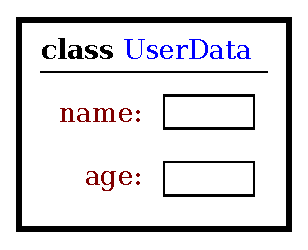
\includegraphics[scale=0.75]{images/class-userdata.eps}
}



An important point is that the static member variables are part of the representation 
of the class in memory.  
Their full names, \code{UserData.name} and \code{UserData.age},
use the name of the class, since they are part of the class. 
When we use class \classname{UserData} to represent the user of the program,
there can only be \textbf{one} user, since we only have memory space to store data about one user. Note that
the class, \code{UserData}, and the variables it contains exist as long as the
program runs. (That is essentially what it means to be ``static.")
Now, consider a similar class that includes some non-static variables:

\displaycode{class PlayerData \{
   static int playerCount;
   String name;
   int age;
\}}\donedisplaycode


\noindent I've also included a static variable in the \classname{PlayerData} class.
Here, the static variable \code{playerCount} is stored as part of the representation of the class in memory.
It's full name is \code{PlayerData.playerCount}, and there is only one of it, which exists
as long as the program runs.  However, the other two variables in the class definition are non-static.
There is no such variable as \code{PlayerData.name} or
\code{PlayerData.age}, since non-static variables do not become part of the
class itself.  But the \classname{PlayerData} class can
be used to create objects.   There can be many objects created using the class, and each 
one will have its \textbf{own} variables called \code{name} and \code{age}.  
This is what it means for the non-static parts of the class to be a template for objects: 
Every object gets its own copy of the non-static part of the class.  We can visualize
the situation in the computer's memory after several object have been created like this:



\par\dumpfigure{
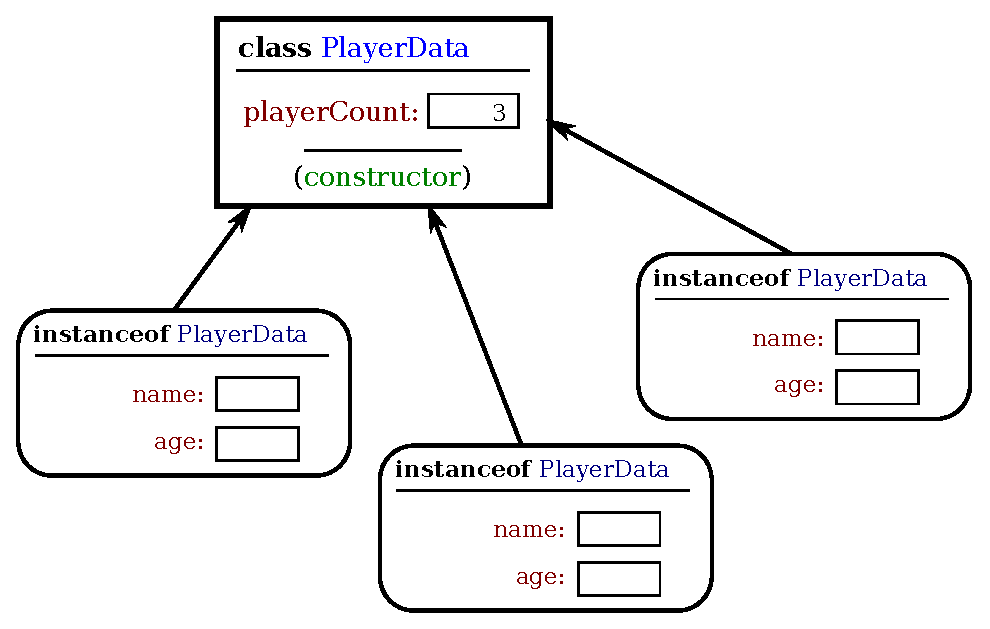
\includegraphics[scale=0.75]{images/instance-of-PlayerData.eps}
}


\noindent Note that the static variable \code{playerCount} is part of the class, and there
is only one copy.  On the other hand, every object contains a \code{name} and an 
\code{age}.  An object that is created from a class is called an \newword{instance} of
that class, and as the picture shows every object ``knows" which class was used to create it.
I've shown class \classname{PlayerData} as containing something called a
``constructor;" the constructor is a subroutine that creates objects.


Now there can
be many ``players" because we can make new objects to represent new players on
demand.  A program might use the \classname{PlayerData} class to store information about multiple
players in a game. Each player has a name and an age. When a player joins the
game, a new \code{PlayerData} object can be created to represent that player.
If a player leaves the game, the \code{PlayerData} object that represents
that player can be destroyed. A system of objects in the program is being used
to \newword{dynamically} model what is happening in the game.
You can't do this with static variables!  ``Dynamic" is the opposite of ``static."


\mybreak



An object that is created using a class is said to be an \newword{instance} 
of that class.  We will sometimes say that the object \newword{belongs} to the class.
The variables that the object contains
are called \newword{instance variables}. The methods (that is, subroutines)
that the object contains are called \newword{instance methods}. 
For example, if the
\code{PlayerData} class, as defined above, is used to create an object, then
that object is an instance of the \code{PlayerData} class, and \code{name}
and \code{age} are instance variables in the object.


My examples here don't include any methods, but methods work similarly to variables.
Static methods are part of the class; non-static, or instance, methods become part of
objects created from the class.  It's not literally true that each object contains
its own copy of the actual compiled code for an instance method. But logically an instance
method is part of the object, and I will continue to say that the object ``contains"
the instance method.


Note that you should distinguish between
the \textbf{source code} for the class, and the \textbf{class itself} (in memory).  The
source code determines both the class and the objects that are created from
that class.  The ``static" definitions in the source code specify the things
that are part of the class itself (in the computer's memory), whereas the non-static definitions in the
source code specify things that will become part of every instance object
that is created from the class.   By the way, static member
variables and static member subroutines in a class are sometimes called
\newword{class variables} and \newword{class methods}, 
since they belong to the class itself, rather than to instances
of that class.


As you can see, the static and the non-static portions of a class are very
different things and serve very different purposes. Many classes contain only
static members, or only non-static, and we will see only a few examples of
classes that contain a mixture of the two.  



\subsection{Fundamentals of Objects}\label{OOP.1.2}

   

So far, I've been talking mostly in generalities, and I haven't given you
much of an idea about what you have to put in a program if you want to work with objects.
Let's look at a specific example to see how it works. Consider this extremely
simplified version of a \code{Student} class, which could be used to store
information about students taking a course:

\displaycode{public class Student \{

   public String name;  // Student's name.
   public double test1, test2, test3;   // Grades on three tests.
   
   public double getAverage() \{  // compute average test grade
      return (test1 + test2 + test3) / 3;
   \}
   
\}  // end of class Student}\donedisplaycode



None of the members of this class are declared to be \code{static}, so the
class exists only for creating objects. This class definition says that any
object that is an instance of the \code{Student} class will include instance
variables named \code{name}, \code{test1}, \code{test2}, and
\code{test3}, and it will include an instance method named
\code{getAverage()}. The names and tests in different objects will generally
have different values. When called for a particular student, the method
\code{getAverage()} will compute an average using \textbf{that
student's} test grades. Different students can have different averages.
(Again, this is what it means to say that an instance method belongs to an
individual object, not to the class.)


In Java, a class is a \textbf{type}, similar to the built-in types
such as \ptype{int} and \ptype{boolean}. So, a class name can be used to
specify the type of a variable in a declaration statement, or the type of a formal
parameter, or the return type of a function. For example, a program could
define a variable named \code{std} of type \code{Student} with the
statement

\displaycode{Student std;}\donedisplaycode


\noindent However, declaring a variable does \textbf{not} create an object!
This is an important point, which is related to this Very Important Fact:

\par
\begin{center}

\textbf{In Java, no variable can ever hold an object.\\
A variable can only hold a reference to an object.}
\end{center}



You should think of objects as floating around independently in the
computer's memory. In fact, there is a special portion of memory called the
\newword{heap} where objects live. Instead of holding an
object itself, a variable holds the information necessary to find the object in
memory. This information is called a \newword{reference} or
\newword{pointer} to the object. In effect, a reference to
an object is the address of the memory location where the object is stored.
When you use a variable of object type, the computer uses the reference in the
variable to find the actual object.


In a program, objects are created using an operator called \code{new}, which
creates an object and returns a reference to that object.  (In fact, the \code{new} operator
calls a special subroutine called a ``constructor" in the class.)
For example, assuming that \code{std} is a variable of type \code{Student}, declared as above,
the assignment statement

\displaycode{std = new Student();}\donedisplaycode


\noindent would create a new object which is an instance of the class
\code{Student}, and it would store a reference to that object in the variable
\code{std}. The value of the variable is a reference, or pointer, to the object.
The object itself is somewhere in the heap.
It is not quite true, then, to say that the object is the ``value
of the variable \code{std}" (though sometimes it is hard to avoid using this
terminology). It is certainly \textbf{not at all true} to say that the
object is ``stored in the variable \code{std}." The proper terminology is that
``the variable \code{std} \newword{refers to} or \newword{points to}
the object," and I will try to stick to that terminology as much as possible.
If I ever say something like ``std \textbf{is} an object," you should read it as
meaning ``std is a variable that refers to an object."


So, suppose that the variable \code{std} refers to an object that is an instance of
class \code{Student}. That object contains instance variables \code{name},
\code{test1}, \code{test2}, and \code{test3}. These instance variables
can be referred to as \code{std.name}, \code{std.test1},
\code{std.test2}, and \code{std.test3}. This follows the usual naming
convention that when \code{B} is part of \code{A}, then the full name of
\code{B} is \code{A.B}. For example, a program might include the lines

\displaycode{System.out.println("Hello, "  +  std.name  +  ".  Your test grades are:");
System.out.println(std.test1);
System.out.println(std.test2);
System.out.println(std.test3);}\donedisplaycode


\noindent This would output the name and test grades from the object to which
\code{std} refers. Similarly, \code{std} can be used to call the
\code{getAverage()} instance method in the object by saying
\code{std.getAverage()}. To print out the student's average, you could
say:

\displaycode{System.out.println( "Your average is "  +  std.getAverage() );}\donedisplaycode



More generally, you could use \code{std.name} any place where a variable
of type \classname{String} is legal. You can use it in expressions. You can assign
a value to it. You can even use it to call subroutines from the \classname{String}
class. For example, \code{std.name.length()} is the number of characters in
the student's name.


It is possible for a variable like \code{std}, whose type is given by a
class, to refer to no object at all. We say in this case that \code{std}
holds a \newword{null pointer} or \newword{null reference}. The null pointer is
written in Java as ``\code{null}". You can store a null reference in the
variable \code{std} by saying

\displaycode{std = null;}\donedisplaycode


\noindent \code{null} is an actual value that is stored in the variable, not a pointer
to something else.  It is \textbf{not} correct to say that the variable ``points to null";
in fact, the variable \textbf{is} null.  For example,
you can test whether the value of \code{std} is null by testing

\displaycode{if (std == null) . . .}\donedisplaycode



If the value of a variable is \code{null}, then it is, of course, illegal
to refer to instance variables or instance methods through that variable---since
there \textbf{is} no object, and hence no instance variables to refer to!  For
example, if the value of the variable \code{std} is \code{null}, then it
would be illegal to refer to \code{std.test1}. If your program attempts to
use a null pointer illegally in this way, the result is an error called a
\newword{null pointer exception}.  When this happens while the program
is running, an exception of type \classname{NullPointerException}
is thrown.



Let's look at a sequence of statements that work with objects:

\displaycode{Student std, std1,       // Declare four variables of
          std2, std3;    //   type Student.

std = new Student();     // Create a new object belonging
                         //   to the class Student, and
                         //   store a reference to that
                         //   object in the variable std.

std1 = new Student();    // Create a second Student object
                         //   and store a reference to
                         //   it in the variable std1.

std2 = std1;             // Copy the reference value in std1
                         //   into the variable std2.

std3 = null;             // Store a null reference in the
                         //   variable std3.
                         
std.name = "John Smith";  // Set values of some instance variables.
std1.name = "Mary Jones";

     // (Other instance variables have default
     //    initial values of zero.)}\donedisplaycode


\noindent After the computer executes these statements, the situation in the
computer's memory looks like this:


\par\dumpfigure{
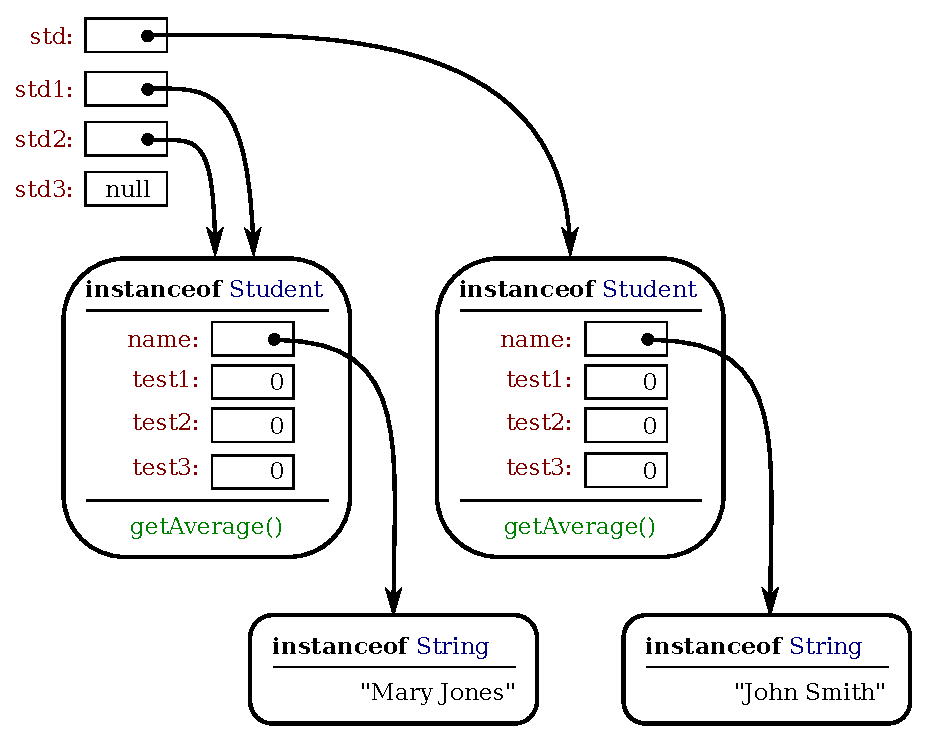
\includegraphics[scale=0.75]{images/objects-in-heap.eps}
}



\noindent In this picture, when a variable
contains a reference to an object, the value of that variable is shown as an
arrow pointing to the object.   Note, by the way, that the \classname{Strings}
are objects!  The variable \code{std3}, with a value of
\code{null}, doesn't point anywhere. The arrows from \code{std1} and
\code{std2} both point to the same object. This illustrates a Very Important
Point:

\par
\begin{center}

\textbf{When one object variable is assigned\\
to another, only a reference is copied.\\
The object referred to is not copied.}
\end{center}


\noindent When the assignment ``\code{std2 = std1};" was executed, no new object was
created. Instead, \code{std2} was set to refer to the very same object that
\code{std1} refers to.   This is to be expected, since the assignment
statement just copies the value that is stored in \code{std1} into 
\code{std2}, and that value is a pointer, not an object.
But this has some consequences that might be surprising.
For example, \code{std1.name} and \code{std2.name} are two different names for the
same variable, namely the instance variable in the object that both
\code{std1} and \code{std2} refer to. After the string \code{"Mary
Jones"} is assigned to the variable \code{\textbf{std1}.name}, it is also
true that the value of \code{\textbf{std2}.name} is \code{"Mary Jones"}.
There is a potential for a lot of confusion here, but you can help protect
yourself from it if you keep telling yourself, ``The object is not in the
variable. The variable just holds a pointer to the object."


You can test objects for equality and inequality using the operators \code{==} and
\code{!=}, but here again, the semantics are different from what you are used to. When
you make a test ``\code{if~(std1~==~std2)}", you are testing whether the
values stored in \code{std1} and \code{std2} are the same. But the values that you are comparing
are references to objects; they are not objects. So, you are testing whether
\code{std1} and \code{std2} refer to the same object, that is, whether they
point to the same location in memory. This is fine, if its what you want to do.
But sometimes, what you want to check is whether the instance variables in the
objects have the same values. To do that, you would need to ask whether 
``\code{std1.test1 == std2.test1 \&\& std1.test2 == std2.test2 \&\&
std1.test3 == std2.test3 \&\& std1.name.equals(std2.name)}".


I've remarked previously that \classname{Strings} are objects, and I've shown
the strings \code{"Mary Jones"} and \code{"John Smith"} as objects in the
above illustration.  (Strings are special objects, treated by Java in a special way, and I
haven't attempted to show the actual internal structure of the \classname{String} objects.)
Since strings are objects, a variable of type \classname{String} can only hold a
reference to a string, not the string itself.  This
explains why using the \code{==} operator to test strings for equality is not
a good idea. Suppose that \code{greeting} is a variable of type
\classname{String}, and that it refers to the string \code{"Hello"}. Then
would the test \code{greeting~==~"Hello"} be true? Well, maybe, maybe not.
The variable \code{greeting} and the \classname{String} literal \code{"Hello"}
each refer to a string that contains the characters H-e-l-l-o. But the strings
could still be different objects, that just happen to contain the same
characters; in that case, \code{greeting~==~"Hello"} would be false.
The function \code{greeting.equals("Hello")} tests whether
\code{greeting} and \code{"Hello"} contain the same characters, which is
almost certainly the question you want to ask. The expression 
\code{greeting~==~"Hello"} tests whether \code{greeting} 
and \code{"Hello"} contain the same characters \textbf{stored in the same memory location}.
(Of course, a \classname{String} variable such as \code{greeting}
can also contain the special value \code{null}, and it \textbf{would} make
sense to use the \code{==} operator to test whether ``\code{greeting~==~null}".)



\mybreak



The fact that variables hold references to objects, not objects themselves,
has a couple of other consequences that you should be aware of. They follow
logically, if you just keep in mind the basic fact that the object is not
stored in the variable. The object is somewhere else; the variable points to it.


Suppose that a variable that refers to an object is declared to be
\code{final}. This means that the value stored in the variable can never be
changed, once the variable has been initialized. The value stored in the
variable is a reference to the object. So the variable will continue to refer
to the same object as long as the variable exists. However, this does not
prevent the data \textbf{in the object} from changing. The variable is
\code{final}, not the object. It's perfectly legal to say

\displaycode{final Student stu = new Student();

stu.name = "John Doe";  // Change data in the object;
                        // The value stored in stu is not changed!
                        // It still refers to the same object.}\donedisplaycode



Next, suppose that \code{obj} is a variable that refers to an object.
Let's consider what happens when \code{obj} is passed as an actual parameter
to a subroutine. The value of \code{obj} is assigned to a formal parameter in
the subroutine, and the subroutine is executed. The subroutine has no power to
change the value stored in the variable, \code{obj}. It only has a copy of
that value. However, the value is a reference to an object. Since the
subroutine has a reference to the object, it can change the data stored \textbf{in} the
object. After the subroutine ends, \code{obj} still points to the same
object, but the data stored \textbf{in the object} might have changed.
Suppose \code{x} is a variable of type \ptype{int} and \code{stu} is a
variable of type \code{Student}. Compare:

\displaycode{void dontChange(int z) \{                void change(Student s) \{
    z = 42;                                  s.name = "Fred";
\}                                       \}

\newcode{The lines:                              The lines:}

   x = 17;                                 stu.name = "Jane";
   dontChange(x);                          change(stu);
   System.out.println(x);                  System.out.println(stu.name);
 
\newcode{output the value 17.                    output the value "Fred".
 
The value of x is \textbf{not}                   The value of stu is not
changed by the subroutine,              changed, but stu.name \textbf{is} changed.
which is equivalent to                  This is equivalent to}

   z = x;                                  s = stu;
   z = 42;                                 s.name = "Fred";}\donedisplaycode

   

   
\subsection{Getters and Setters}\label{OOP.1.3}



When writing new classes, it's a good idea to pay attention to the issue
of access control.  Recall that making a member of a class \code{public}
makes it accessible from anywhere, including from other classes.  On the
other hand, a \code{private} member can only be used in the class
where it is defined.
   

In the opinion of many programmers, almost all member variables should
be declared \code{private}.  This gives you complete control over what
can be done with the variable.  Even if the variable itself is private,
you can allow other classes to find out what its value is by providing
a \code{public} \newword{accessor method} that returns the
value of the variable.  For example, if your class contains a \code{private}
member variable, \code{title}, of type \classname{String}, you
can provide a method

\displaycode{public String getTitle() \{
    return title;
\}}\donedisplaycode


   
\noindent that returns the value of \code{title}.  By convention, the name of
an accessor method for a variable is obtained by capitalizing the name of variable and
adding ``get" in front of the name.  So, for the variable \code{title}, we get
an accessor method named ``get" \code{+} ``Title", or \code{getTitle()}.
Because of this naming convention, accessor methods are more often referred to
as \newword{getter methods}.  A getter method provides ``read access" to
a variable.  (Sometimes for \ptype{boolean} variables, ``is" is used in place
of ``get".  For example, a getter for a \ptype{boolean} member variable named
\code{done} might be called \code{isDone()}.)
   

You might also want to allow ``write access" to a \code{private} variable.
That is, you might want to make it possible for other classes to specify a new value
for the variable.  This is done with a \newword{setter method}.  (If you don't
like simple, Anglo-Saxon words, you can use the fancier term \newword{mutator method}.)
The name of a setter method should consist of ``set" followed by a capitalized copy of
the variable's name, and it should have a parameter with the same type as the
variable.  A setter method for the variable \code{title} could be written
   
\displaycode{public void setTitle( String newTitle ) \{
   title = newTitle;
\}}\donedisplaycode

   

It is actually very common to provide both a getter and a setter method for
a private member variable.  Since this allows other classes both to see and to
change the value of the variable, you might wonder why not just make the
variable \code{public}?  The reason is that getters and setters are not
restricted to simply reading and writing the variable's value.  In fact,
they can take any action at all.  For example, a getter method might keep
track of the number of times that the variable has been accessed:

\displaycode{public String getTitle() \{
    titleAccessCount++;  // Increment member variable titleAccessCount.
    return title;
\}}\donedisplaycode


\noindent and a setter method might check that the value that is being
assigned to the variable is legal:
   
\displaycode{public void setTitle( String newTitle ) \{
   if ( newTitle == null )   // Don't allow null strings as titles!
      title = "(Untitled)";  // Use an appropriate default value instead.
   else
      title = newTitle;
\}}\donedisplaycode

   
\noindent Even if you can't think of any extra chores to do in a getter or setter
method, you might change your mind in the future when you redesign and
improve your class.  If you've used a getter and setter from the beginning,
you can make the modification to your class without affecting any of the
classes that use your class.  The \code{private} member variable
is not part of the public interface of your class; only the \code{public}
getter and setter methods are, and you are free to change their implementations
without changing the public interface of your class.
If you \textbf{haven't} used get and set from
the beginning, you'll have to contact everyone who uses your class and
tell them, ``Sorry people, you'll have to track down every use that you've
made of this variable and change your code to use my new get and set
methods instead."
   

A couple of final notes:  Some advanced aspects of Java rely on the
naming convention for getter and setter methods, so it's a good idea to
follow the convention rigorously.  And though I've been talking about using
getter and setter methods for a variable, you can define get and set
methods even if there is no variable.  A getter and/or setter method defines
a \newword{property} of the class, that might or might not correspond
to a variable.  For example, if a class includes a \code{public} \code{void}
instance method with signature \code{setValue(double)}, then the class
has a ``property" named \code{value} of type \ptype{double}, and
it has this property whether or not the class has a member variable
named \code{value}.




\subsection{Arrays and Objects}\label{OOP.1.4}



As I noted in Subsection~\ref{control.7a.1}, arrays are objects.  Like \classname{Strings}
they are special objects, with their own unique syntax.  An array type such as
\atype{int\hbox{[\hskip2pt]}} or \atype{String\hbox{[\hskip2pt]}} is actually a class, and arrays
are created using a special version of the \code{new} operator.
As in the case for other object variables,  an array variable can never
hold an actual array---only a reference to an array object.  The array object 
itself exists in the heap.  It is possible for an array variable to hold the value
\code{null}, which means there is no actual array.


For example, suppose that \code{list} is a variable of type \atype{int\hbox{[\hskip2pt]}}.
If the value of \code{list} is \code{null}, then any attempt to access
\code{list.length} or an array element \code{list[i]} would be an error
and would cause an exception of type \classname{NullPointerException}.  If
\code{newlist} is another variable of type \atype{int\hbox{[\hskip2pt]}}, then the
assignment statement

\displaycode{newlist = list;}\donedisplaycode


\noindent only copies the reference value in \code{list} into \code{newlist}.
If \code{list} is \code{null}, the result is that \code{newlist} will also be \code{null}.
If \code{list} points to an array, the assignment statement does \textbf{not} make a copy of the
array.  It just sets \code{newlist} to refer to the same array as \code{list}.  For
example, the output of the following code segment

\displaycode{list = new int[3];
list[1] = 17;
newlist = list; // newlist points to the same array as list!
newlist[1] = 42;
System.out.println( list[1] );}\donedisplaycode


\noindent would be 42, not 17, since \code{list[1]} and \code{newlist[1]} are just different names
for the same element in the array.  All this is very natural, once you understand that
arrays are objects and array variables hold pointers to arrays.


This fact also comes into play when an array is passed as a parameter to a subroutine.
The value that is copied into the subroutine is a pointer to the array.  The array is
not copied.  Since the subroutine has a reference to the original array, any changes that
it makes to elements of the array are being made to the original and will persist after
the subroutine returns.


\mybreak



Arrays are objects.  They can also hold objects.
The base type of an array can be a class.  We have already seen this when we used
arrays of type \atype{String\hbox{[\hskip2pt]}}, but any class can be used as the base type.
For example, suppose \classname{Student} is the class defined earlier in
this section.  Then we can have arrays of type \atype{Student\hbox{[\hskip2pt]}}.  For an array
of type \atype{Student\hbox{[\hskip2pt]}}, each element of the array is a variable of type
\classname{Student}.  To store information about 30 students,
we could use an array

\displaycode{Student[] classlist;  // Declare a variable of type Student[].
classlist = new Student[30];  // The variable now points to an array.}\donedisplaycode


\noindent The array has 30 elements, \code{classlist[0]}, \code{classlist[1]}, 
\dots \code{classlist[29]}.  When the array is created, it is filled with the
default initial value, which for an object type is \code{null}.  So, although
we have 30 array elements of type \classname{Student}, we don't yet have
any actual \classname{Student} objects!  All we have is 30 nulls.
If we want student objects, we have to create them:

\displaycode{Student[] classlist;
classlist = new Student[30];
for ( int i = 0; i \< 30; i++ ) \{
    classlist[i] = new Student();
\}}\donedisplaycode


\noindent Once we have done this, each \code{classlist[i]} points to an object of type
\classname{Student}.  If we want to talk about the name of student number 3,
we can use \code{classlist[3].name}.  The average for student number \code{i}
can be computed by calling \code{classlist[i].getAverage()}.  You can do anything
with \code{classlist[i]} that you could do with any other variable of type
\classname{Student}.




   



\section{Constructors and Object Initialization}\label{OOP.2}



\start{{\Large O}bject types in Java} are very different from the
primitive types. Simply declaring a variable whose type is given as a class
does not automatically create an object of that class. Objects must be
explicitly \newword{constructed}. For the computer, the
process of constructing an object means, first, finding some unused memory in
the heap that can be used to hold the object and, second, filling in the
object's instance variables. As a programmer, you don't care where in memory
the object is stored, but you will usually want to exercise some control over
what initial values are stored in a new object's instance variables. In many
cases, you will also want to do more complicated initialization or bookkeeping
every time an object is created.
   
\subsection{Initializing Instance Variables}\label{OOP.2.1}



An instance variable can be assigned an initial value in its declaration,
just like any other variable. For example, consider a class named
\classname{PairOfDice}. An object of this class will represent a pair of dice. It
will contain two instance variables to represent the numbers showing on the
dice and an instance method for rolling the dice:

\displaycode{public class PairOfDice \{

    public int die1 = 3;   // Number showing on the first die.
    public int die2 = 4;   // Number showing on the second die.

    public void roll() \{
            // Roll the dice by setting each of the dice to be
            // a random number between 1 and 6.
         die1 = (int)(Math.random()*6) + 1;
         die2 = (int)(Math.random()*6) + 1;
    \}
    
\} // end class PairOfDice}\donedisplaycode


\noindent The instance variables \code{die1} and \code{die2} are initialized to
the values 3 and 4 respectively. These initializations are executed whenever a
\classname{PairOfDice} object is constructed. It's important to understand when
and how this happens. There can be many \classname{PairOfDice} objects. Each time
one is created, it gets its own instance variables, and the assignments
``\code{die1~=~3}" and ``\code{die2~=~4}" are executed to fill in the values
of those variables. To make this clearer, consider a variation of the
\classname{PairOfDice} class:

\displaycode{public class PairOfDice \{

    public int die1 = (int)(Math.random()*6) + 1;
    public int die2 = (int)(Math.random()*6) + 1;
 
    public void roll() \{
         die1 = (int)(Math.random()*6) + 1;
         die2 = (int)(Math.random()*6) + 1;
    \}
    
\} // end class PairOfDice}\donedisplaycode


\noindent Here, every time a new \classname{PaifOfDice} is created,
the dice are initialized to random values, as if a new pair of dice
were being thrown onto the gaming table. Since the initialization is executed
for each new object, a set of random initial values will be computed for each
new pair of dice. Different pairs of dice can have different initial values.
For initialization of \textbf{static} member variables, of course, the situation
is quite different. There is only one copy of a \code{static} variable, and
initialization of that variable is executed just once, when the class is first
loaded.
   

If you don't provide any initial value for an instance variable, a default
initial value is provided automatically. Instance variables of numerical type
(\ptype{int}, \ptype{double}, etc.) are automatically initialized to zero if
you provide no other values; \ptype{boolean} variables are initialized to
\code{false}; and \ptype{char} variables, to the Unicode character with code
number zero. An instance variable can also be a variable of object type. For
such variables, the default initial value is \code{null}. (In particular,
since \code{Strings} are objects, the default initial value for
\classname{String} variables is \code{null}.)


   
\subsection{Constructors}\label{OOP.2.2}



Objects are created with the operator, \code{new}. For example, a program
that wants to use a \classname{PairOfDice} object could say:

\displaycode{PairOfDice dice;   // Declare a variable of type PairOfDice.

dice = new PairOfDice();  // Construct a new object and store a
                          //   reference to it in the variable.}\donedisplaycode



In this example, ``\code{new PairOfDice()}" is an expression that allocates
memory for the object, initializes the object's instance variables, and then
returns a reference to the object. This reference is the value of the
expression, and that value is stored by the assignment statement in the
variable, \code{dice}, so that after the assignment statement is
executed, \code{dice} refers to the newly created object.
Part of this expression, ``\code{PairOfDice()}",
looks like a subroutine call, and that is no accident. It is, in fact, a call
to a special type of subroutine called a \newword{constructor}. 
This might puzzle you, since there is no such
subroutine in the class definition. However, every class has at least one
constructor. If the programmer doesn't write a constructor definition in a 
class, then the system will provide a 
\newword{default constructor} for that class. 
This default constructor does nothing
beyond the basics: allocate memory and initialize instance variables. If you
want more than that to happen when an object is created, you can include one or
more constructors in the class definition.


The definition of a constructor looks much like the definition of any other
subroutine, with three exceptions. A constructor does not have any return type
(not even \code{void}). The name of the constructor must be the same as the
name of the class in which it is defined. And the only modifiers that can be used
on a constructor definition are the access modifiers \code{public},
\code{private}, and \code{protected}. (In particular, a constructor can't
be declared \code{static}.)


However, a constructor does have a subroutine body of the usual form, a
block of statements. There are no restrictions on what statements can be used.
And a constructor can have a list of formal parameters. In fact, the ability to include
parameters is one of the main reasons for using constructors. The parameters
can provide data to be used in the construction of the object. For example, a
constructor for the \classname{PairOfDice} class could provide the values that are
initially showing on the dice. Here is what the class would look like in that
case:

\displaycode{public class PairOfDice \{

    public int die1;   // Number showing on the first die.
    public int die2;   // Number showing on the second die.
    
    public PairOfDice(int val1, int val2) \{
            // Constructor.  Creates a pair of dice that
            // are initially showing the values val1 and val2.
         die1 = val1;  // Assign specified values 
         die2 = val2;  //           to the instance variables.
    \}

    public void roll() \{
            // Roll the dice by setting each of the dice to be
            // a random number between 1 and 6.
         die1 = (int)(Math.random()*6) + 1;
         die2 = (int)(Math.random()*6) + 1;
    \}
    
\} // end class PairOfDice}\donedisplaycode



The constructor is declared as ``\code{public PairOfDice(int val1, int
val2)~...}", with no return type and with the same name as the name of the
class. This is how the Java compiler recognizes a constructor. The constructor
has two parameters, and values for these parameters must be provided when the
constructor is called. For example, the expression ``\code{new~PairOfDice(3,4)}"
would create a \classname{PairOfDice} object in which the
values of the instance variables \code{die1} and \code{die2} are initially
3 and~4. Of course, in a program, the value returned by the constructor should
be used in some way, as in

\displaycode{PairOfDice dice;            // Declare a variable of type PairOfDice.

dice = new PairOfDice(1,1); // Let dice refer to a new PairOfDice
                            //   object that initially shows 1, 1.}\donedisplaycode



Now that we've added a constructor to the \classname{PairOfDice} class, we can
no longer create an object by saying ``\code{new PairOfDice()}"! The system
provides a default constructor for a class \textbf{only} if the class
definition does not already include a constructor.  In this version of \classname{PairOfDice},
there is only one
constructor in the class, and it requires two actual parameters.
However, this is not a big
problem, since we can add a second constructor to the class, one that has no
parameters. In fact, you can have as many different constructors as you want,
as long as their signatures are different, that is, as long as they have
different numbers or types of formal parameters. In the \classname{PairOfDice}
class, we might have a constructor with no parameters which produces a pair of
dice showing random numbers:

\displaycode{public class PairOfDice \{

    public int die1;   // Number showing on the first die.
    public int die2;   // Number showing on the second die.
    
    public PairOfDice() \{
            // Constructor.  Rolls the dice, so that they initially
            // show some random values.
        roll();  // Call the roll() method to roll the dice.
    \}
    
    public PairOfDice(int val1, int val2) \{
            // Constructor.  Creates a pair of dice that
            // are initially showing the values val1 and val2.
        die1 = val1;  // Assign specified values 
        die2 = val2;  //            to the instance variables.
    \}

    public void roll() \{
            // Roll the dice by setting each of the dice to be
            // a random number between 1 and 6.
        die1 = (int)(Math.random()*6) + 1;
        die2 = (int)(Math.random()*6) + 1;
    \}

\} // end class PairOfDice}\donedisplaycode


\noindent Now we have the option of constructing a \classname{PairOfDice} object either
with ``\code{new PairOfDice()}" or with ``\code{new PairOfDice(x,y)}", where
\code{x} and \code{y} are \ptype{int}-valued expressions.


This class, once it is written, can be used in any program that needs to
work with one or more pairs of dice. None of those programs will ever have to
use the obscure incantation ``\code{(int)(Math.random()*6)+1}", because it's
done inside the \classname{PairOfDice} class. And the programmer, having once
gotten the dice-rolling thing straight will never have to worry about it again.
Here, for example, is a main program that uses the \classname{PairOfDice} class to
count how many times two pairs of dice are rolled before the two pairs come up
showing the same value.  This illustrates once again that you can create several
instances of the same class:

\displaycode{public class RollTwoPairs \{

    public static void main(String[] args) \{
                 
        PairOfDice firstDice;  // Refers to the first pair of dice.
        firstDice = new PairOfDice();
        
        PairOfDice secondDice; // Refers to the second pair of dice.
        secondDice = new PairOfDice();
        
        int countRolls;  // Counts how many times the two pairs of
                         //    dice have been rolled.
        
        int total1;      // Total showing on first pair of dice.
        int total2;      // Total showing on second pair of dice.
        
        countRolls = 0;
        
        do \{  // Roll the two pairs of dice until totals are the same.
        
            firstDice.roll();    // Roll the first pair of dice.
            total1 = firstDice.die1 + firstDice.die2;   // Get total.
            System.out.println("First pair comes up  " + total1);
            
            secondDice.roll();    // Roll the second pair of dice.
            total2 = secondDice.die1 + secondDice.die2;   // Get total.
            System.out.println("Second pair comes up " + total2);
            
            countRolls++;   // Count this roll.
            
            System.out.println();  // Blank line.
            
        \} while (total1 != total2);
        
        System.out.println("It took " + countRolls 
                          + " rolls until the totals were the same.");
        
    \} // end main()

\} // end class RollTwoPairs}\donedisplaycode


   

\mybreak

   

Constructors are subroutines, but they are subroutines of a special type.
They are certainly not instance methods, since they don't belong to objects.
Since they are responsible for creating objects, they exist before any objects
have been created. They are more like \code{static} member subroutines, but
they are not and cannot be declared to be \code{static}. In fact, according
to the Java language specification, they are technically not members of the
class at all!  In particular, constructors are not referred to as
``methods."


Unlike other subroutines, a constructor can only be called using the
\code{new} operator, in an expression that has the form

\displaycode{new \bnf{class-name} ( \bnf{parameter-list} )}\donedisplaycode


\noindent where the \bnf{parameter-list} is possibly empty.
I call this an expression because it computes and returns a value, namely a
reference to the object that is constructed. Most often, you will store the
returned reference in a variable, but it is also legal to use a constructor
call in other ways, for example as a parameter in a subroutine call or as part
of a more complex expression. Of course, if you don't save the reference in a
variable, you won't have any way of referring to the object that was just
created.


A constructor call is more complicated than an ordinary subroutine or
function call. It is helpful to understand the exact steps that the computer
goes through to execute a constructor call:



\mynumberedlist{

\mynumbereditem First, the computer gets a block of unused memory in the heap, large enough
to hold an object of the specified type.
\mynumbereditem It initializes the instance variables of the object. If the declaration of
an instance variable specifies an initial value, then that value is computed
and stored in the instance variable. Otherwise, the default initial value is
used.
\mynumbereditem The actual parameters in the constructor, if any, are evaluated, and the
values are assigned to the formal parameters of the constructor.
\mynumbereditem The statements in the body of the constructor, if any, are executed.
\mynumbereditem A reference to the object is returned as the value of the constructor
call.
}



The end result of this is that you have a reference to a newly constructed
object.


\mybreak



For another example, let's rewrite the \classname{Student} class that was used
in \weblink{s1.html}{Section 1}. I'll add a constructor, and I'll also take
the opportunity to make the instance variable, \code{name}, private.

\displaycode{public class Student \{

   private String name;                 // Student's name.
   public double test1, test2, test3;   // Grades on three tests.
   
   Student(String theName) \{
        // Constructor for Student objects;
        // provides a name for the Student.
        // The name can't be null.
      if ( theName == null )
          throw new IllegalArgumentException("name can't be null");
      name = theName;
   \}
   
   public String getName() \{
        // Getter method for reading the value of the private
        // instance variable, name.
      return name;
   \}
   
   public double getAverage() \{ 
        // Compute average test grade.
      return (test1 + test2 + test3) / 3;
   \}

\}  // end of class Student}\donedisplaycode



An object of type \classname{Student} contains information about some
particular student. The constructor in this class has a parameter of type
\classname{String}, which specifies the name of that student. Objects of type
\classname{Student} can be created with statements such as:

\displaycode{std = new Student("John Smith");
std1 = new Student("Mary Jones");}\donedisplaycode


\noindent In the original version of this class, the value of \code{name} had to be
assigned by a program after it created the object of type \classname{Student}.
There was no guarantee that the programmer would always remember to set the
\code{name} properly. In the new version of the class, there is no way to
create a \classname{Student} object except by calling the constructor, and that
constructor automatically sets the \code{name}. Furthermore, the constructor makes
it impossible to have a student object whose name is \code{null}.
The programmer's life is made
easier, and whole hordes of frustrating bugs are squashed before they even have
a chance to be born.


Another type of guarantee is provided by the \code{private} modifier.
Since the instance variable, \code{name}, is \code{private}, there is no
way for any part of the program outside the \classname{Student} class to get at
the \code{name} directly. The program sets the value of \code{name},
indirectly, when it calls the constructor. I've provided a getter function,
\code{getName()}, that can be used from outside the class to find out the
\code{name} of the student. But I haven't provided any setter method or other way to change the
name. Once a student object is created, it keeps the same name as long as it
exists.


Note that it would be legal, and good style, to declare the variable \code{name} to be
``\code{final}" in this class.  An instance variable can be \code{final}
provided it is either assigned a value in its declaration or is assigned a value
in every constructor in the class.  It is illegal to assign a value to a \code{final}
instance variable, except inside a constructor.


\mybreak



Let's take this example a little farther to illustrate one more aspect
of classes:  What happens when you mix static and non-static in the same class?
In that case, it's legal for an instance method in the class to use static member
variables or call static member subroutines.  An object knows what class it belongs
to, and it can refer to static members of that class.  But there it only 
one copy of the static member, in the class itself.  Effectively, all the
objects share one copy of the static member.


As an example, consider a version of the \classname{Student}
class to which I've added an \code{ID} for each
student and a \code{static} member called \code{nextUniqueID}. Although
there is an \code{ID} variable in each student object, there is only one
\code{nextUniqueID} variable.

\displaycode{public class Student \{

   private String name;                 // Student's name.
   public double test1, test2, test3;   // Grades on three tests.
   
   \newcode{private int ID;  // Unique ID number for this student.}

   \newcode{private static int nextUniqueID = 0;
             // keep track of next available unique ID number}
   
   Student(String theName) \{
        // Constructor for Student objects; provides a name for the Student,
        // \newcode{and assigns the student a unique ID number.}
      name = theName;
      \newcode{nextUniqueID++;
      ID = nextUniqueID;}
   \}
   
   public String getName() \{
        // Getter method for reading the value of the private
        // instance variable, name.
      return name;
   \}
   
   \newcode{public int getID() \{
        // Getter method for reading the value of ID.
      return ID;
   \}}
   
   public double getAverage() \{  
        // Compute average test grade.
      return (test1 + test2 + test3) / 3;
   \}
   
\}  // end of class Student}\donedisplaycode



Since \code{nextUniqueID} is a \code{static} variable,
the initialization ``\code{nextUniqueID~=~0}" is done only once, when the
class is first loaded. Whenever a \classname{Student} object is constructed and
the constructor says ``\code{nextUniqueID++;}", it's always the same static
member variable that is being incremented. When the very first \classname{Student}
object is created, \code{nextUniqueID} becomes 1. When the second object is
created, \code{nextUniqueID} becomes 2. After the third object, it becomes 3.
And so on. The constructor stores the new value of \code{nextUniqueID} in the
\code{ID} variable of the object that is being created. Of course,
\code{ID} is an instance variable, so every object has its own individual
\code{ID} variable. The class is constructed so that each student will
automatically get a different value for its \code{ID} variable. Furthermore,
the \code{ID} variable is \code{private}, so there is no way for this
variable to be tampered with after the object has been created. You are
guaranteed, just by the way the class is designed, that every student object
will have its own permanent, unique identification number. Which is kind of
cool if you think about it.


(Unfortunately, if you think about it a bit more, it turns out that the
guarantee isn't quite absolute.  The guarantee is valid in programs that use
a single thread.  But, as a preview of the difficulties of parallel programming, 
I'll note that in multi-threaded programs, where several things can be
going on at the same time, things can get a bit strange.  In a multi-threaded
program, it is possible that two threads are creating \classname{Student}
objects at exactly the same time, and it becomes possible for both objects to get
the same ID number.  We'll come back to this in Subsection~\ref{threads.1.3}, where 
you will learn how to fix the problem.)




\subsection{Garbage Collection}\label{OOP.2.3}



So far, this section has been about creating objects. What about destroying
them? In Java, the destruction of objects takes place automatically.


An object exists in the heap, and it can be accessed only through variables
that hold references to the object. What should be done with an object if there
are no variables that refer to it? Such things can happen. Consider the
following two statements (though in reality, you'd never do anything like
this in consecutive statements!):

\displaycode{Student std = new Student("John Smith");
std = null;}\donedisplaycode


\noindent In the first line, a reference to a newly created \classname{Student} object is
stored in the variable \code{std}. But in the next line, the value of
\code{std} is changed, and the reference to the \classname{Student} object is
gone. In fact, there are now no references whatsoever to that object, in
any variable. So there is no way for the program ever to use the object again!
It might as well not exist. In fact, the memory occupied by the object should
be reclaimed to be used for another purpose.


Java uses a procedure called \newword{garbage collection}
to reclaim memory occupied by objects that are no longer accessible to a
program. It is the responsibility of the system, not the programmer, to keep
track of which objects are ``garbage." In the above example, it was very easy to
see that the \classname{Student} object had become garbage. Usually, it's much
harder. If an object has been used for a while, there might be several
references to the object stored in several variables. The object doesn't become
garbage until all those references have been dropped.


In many other programming languages, it's the programmer's responsibility to
delete the garbage. Unfortunately, keeping track of memory usage is very
error-prone, and many serious program bugs are caused by such errors. A
programmer might accidently delete an object even though there are still
references to that object. This is called a \newword{dangling pointer error}, 
and it leads to problems when the program tries to access
an object that is no longer there. Another type of error is a \newword{memory leak}, 
where a programmer neglects to delete objects
that are no longer in use. This can lead to filling memory with objects that
are completely inaccessible, and the program might run out of memory even
though, in fact, large amounts of memory are being wasted.


Because Java uses garbage collection, such errors are simply impossible.
Garbage collection is an old idea and has been used in some programming
languages since the 1960s. You might wonder why all languages don't use garbage
collection. In the past, it was considered too slow and wasteful. However,
research into garbage collection techniques combined with the incredible speed
of modern computers have combined to make garbage collection feasible.
Programmers should rejoice.
   



   



\section{Programming with Objects}\label{OOP.3}




\start{{\Large T}here are several ways} in which object-oriented
concepts can be applied to the process of designing and writing programs. The
broadest of these is \newword{object-oriented analysis and design} 
which applies an object-oriented methodology to the earliest
stages of program development, during which the overall design of a program is
created. Here, the idea is to identify things in the problem domain that can be
modeled as objects. On another level, object-oriented programming encourages
programmers to produce \newword{generalized software components} 
that can be used in a wide variety of programming projects.
   
   

Of course, for the most part, you will experience ``generalized software
components" by using the standard classes that come along with Java.  We begin
this section by looking at some built-in classes that are used for creating
objects.  At the end of the section, we will get back to generalities.

\subsection{Some Built-in Classes}\label{OOP.3.1}



Although the focus of object-oriented programming is generally on the design
and implementation of new classes, it's important not to forget that the
designers of Java have already provided a large number of reusable classes.
Some of these classes are meant to be extended to produce new classes, while
others can be used directly to create useful objects. A true mastery of Java
requires familiarity with a large number of built-in classes---something that
takes a lot of time and experience to develop. Let's take a moment to look at a 
few built-in classes that you might find useful.


A string can be built up from smaller pieces using the \code{+} operator,
but this is not always efficient. If \code{str} is a \classname{String} and
\code{ch} is a character, then executing the command
``\code{str~= str~+~ch;}" involves creating a whole new
string that is a copy of \code{str}, with the value of \code{ch} appended
onto the end. Copying the string takes some time. Building up a long string
letter by letter would require a surprising amount of processing. The class
\classname{StringBuilder} makes it possible to be efficient about
building up a long string from a number of smaller pieces.  To do this,
you must make an object belonging to the \classname{StringBuilder}
class.  For example:
   
\displaycode{StringBuilder builder = new StringBuilder();}\donedisplaycode

   
\noindent (This statement both declares the variable \code{builder} and initializes
it to refer to a newly created \classname{StringBuilder} object.  Combining
declaration with initialization was covered in Subsection~\ref{subroutines.7.1} and works
for objects just as it does for primitive types.) 
   
 
Like a \classname{String}, a \classname{StringBuilder} 
contains a sequence of characters.
However, it is possible to add new characters onto the end of a
\code{StringBuilder} without continually making copies of the data that it already
contains. If
\code{x} is a value of any type and \code{builder} is the variable
defined above, then the command \code{builder.append(x)}
will add \code{x}, converted into a string representation, onto the end of
the data that was already in the builder.  This can be done more efficiently than
copying the data every time something is appended. A~long
string can be built up in a \classname{StringBuilder} using a sequence of
\code{append()} commands. When the string is complete, the function
\code{builder.toString()} will return a copy of the string in the builder as an
ordinary value of type \classname{String}. The \classname{StringBuilder}
class is in the standard package \code{java.lang}, so you can use its simple name without
importing it.


A number of useful classes are collected in the package \code{java.util}.
For example, this package contains classes for working with collections of
objects.  We
will study such collection classes extensively in Chapter~\ref{generics}.
Another class in this package, \code{java.util.Date}, is
used to represent times. When a \code{Date} object is constructed without
parameters, the result represents the current date and time, so an easy way to
display this information is:

\displaycode{System.out.println( new Date() );}\donedisplaycode


\noindent Of course, since it is in the package \code{java.util},
in order to use the \code{Date} class in your program, you must make it
available by importing it with one of the statements
``\code{import~java.util.Date;}" or ``\code{import~java.util.*;}"
at the beginning of your program. (See Subsection~\ref{subroutines.5.3}
for a discussion of packages and \code{import}.)


I will also mention the class \code{java.util.Random}. An object
belonging to this class is a \textit{source} of random numbers (or, more precisely
pseudorandom numbers).  The standard
function \code{Math.random()} uses one of these objects behind the scenes to
generate its random numbers. An object of type \code{Random} can generate
random integers, as well as random real numbers. If \code{randGen} is created
with the command:

\displaycode{Random randGen = new Random();}\donedisplaycode


\noindent and if \code{N} is a positive integer, then \code{randGen.nextInt(N)}
generates a random integer in the range from \code{0} to \code{N-1}. For
example, this makes it a little easier to roll a pair of dice. Instead of
saying ``\code{die1~= (int)(6*Math.random())+1;}", one can say
``\code{die1~= randGen.nextInt(6)+1;}". (Since you also have to
import the class \code{java.util.Random} and create the \code{Random}
object, you might not agree that it is actually easier.)  An object of
type \code{Random} can also be used to generate so-called
Gaussian distributed random real numbers.


Many of Java's standard classes are used in GUI programming. You will encounter
a number of them in the Chapter~\ref{GUI1}.  Here, I will mention only
the class \classname{Color},
from the package \code{java.awt}, so that I can use it in the next example.
A \classname{Color} object represents a 
color that can be used for drawing.  In Section~\ref{control.8}, you encountered
color constants such as \code{Color.RED}.  These constants are final, static member
variables in the \classname{Color} class, and their values are objects of type
\classname{Color}.  It is also possible to create new color objects.  Class
\classname{Color} has several constructors.  One of them, which is called
as \code{new~Color(r,g,b)}, takes three integer parameters to specify the
red, green, and blue components of the color.  The parameters must be in the range 0
to 255.  Another constructor, \code{new~Color(r,g,b,t)}, adds a fourth
integer parameter, which must also be in the range 0 to 255.  The fourth parameter
determines how transparent or opaque the color is.  When you draw with a transparent
color, the background shows through the color to some extent.  A larger value of
the parameter \code{t} gives a color that is less transparent and more opaque.
(If you know hexadecimal color codes, there is a constructor for you.  It takes one
parameter of type \ptype{int} that encodes all the color components.
For example, \code{new~Color(0x8B5413)} creates a brown color.)


A \classname{Color} object has only a few instance methods that you
are likely to use.  Mainly, there are functions like \code{getRed()} to
get the individual color components of the color.  There are no ``setter" methods
to change the color components.  In fact, a \classname{Color} is
an \newword{immutable} object, meaning that all of its instance variables
are \code{final} and cannot be changed after the object is created.
\classname{Strings} are another example of immutable objects, and we
will make some of our own later in this section.
   

The main point of all this, again, is that many problems have already been solved,
and the solutions are available in Java's standard classes. If you are faced
with a task that looks like it should be fairly common, it might be worth
looking through a Java reference to see whether someone has already written a
class that you can use.



\subsection{The class ``Object"}\label{OOP.3.3}



We have already seen that one of the major features of object-oriented programming
is the ability to create subclasses of a class.   The subclass inherits all the properties
or behaviors of the class, but can modify and add to what it inherits.  In Section~\ref{OOP.5},
you'll learn how to create subclasses.   What you don't
know yet is that \textbf{every} class in Java (with just one exception) is a subclass
of some other class.  If you create a class and don't explicitly make it a subclass of
some other class, then it automatically becomes a subclass of the special class
named \classname{Object}.  (\classname{Object} is the one class
that is not a subclass of any other class.)


Class \classname{Object} defines several instance methods that are inherited by
every other class.  These methods can be used with any object whatsoever. I will mention
just one of them here.  You will encounter more of them later in the book.
   

The instance method \code{toString()} in class \classname{Object} returns
a value of type \classname{String} that is supposed to be a string representation
of the object.  You've already used this method implicitly,  any time you've printed out an object or
concatenated an object onto a string.  When you use an object in a context that requires a
string, the object is automatically converted to type \classname{String} 
by calling its \code{toString()} method.


The version of \code{toString} that is defined in \classname{Object} just returns
the name of the class that the object belongs to, concatenated with a code number called the
\newword{hash code} of the object; this is not very useful. When you create a class,
you can write a new \code{toString()} method for it, which will replace the inherited
version.  For example, we might add the following method to any of the \classname{PairOfDice}
classes from the previous section:

\displaycode{/**
 * Return a String representation of a pair of dice, where die1
 * and die2 are instance variables containing the numbers that are
 * showing on the two dice.
 */
public String toString() \{
   if (die1 == die2)
      return "double " + die1;
   else
      return die1 + " and " + die2;
\}}\donedisplaycode

   
\noindent If \code{dice} refers to a \classname{PairOfDice} object, then
\code{dice.toString()} will return strings such as ``3~and~6",
``5~and~1", and ``double~2", depending on the numbers showing on the dice.
This method would be used automatically to convert \code{dice} to type
\classname{String} in a statement such as
   
\displaycode{System.out.println( "The dice came up " + dice );}\donedisplaycode

   
\noindent so this statement might output, ``The dice came up 5 and~1" or ``The
dice came up double 2".  You'll see another example of a \code{toString()}
method in the next section.
   


   
\subsection{Writing and Using a Class}\label{OOP.3.2}



As an example, we will write an animation program, based on the same
animation framework that was used in Subsection~\ref{control.8.3}.  The animation
shows a number of semi-transparent disk that grow in size as the
animation plays.  The disks have random colors and locations.  When a disk gets too
big, or sometimes just at random, the disk disappears and is replaced with a
new disk at a random location.  Here is a screenshot from the program:



\par\dumpfigure{
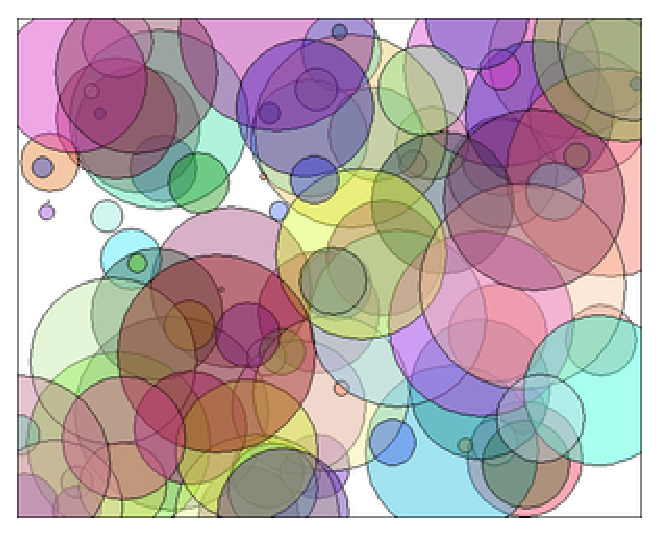
\includegraphics[scale=0.6]{images/growing-circles.eps}
}

      
\noindent A disk in this program can be represented as an object.  A disk has properties---color,
location, and size---that can be instance variables in the object.  As for instance
methods, we need to think about what we might want to do with a disk.  An obvious candidate
is that we need to be able to draw it, so we can include an instance method
\code{draw(g)}, where \code{g} is a graphics context that will be used to
do the drawing.  The class can also include one or more constructors.  A constructor
initializes the object.  It's not always clear what data should be provided as parameters
to the constructors.  In this case, as an example,
the constructor's parameters specify the location and size for
the circle, but the constructor makes up a color using random values for the red, green,
and blue components.  Here's the complete class:

\displaycode{import java.awt.Color;  // import some standard GUI classes
import java.awt.Graphics;

/**
 * A simple class that holds the size, color, and location of a colored disk,
 * with a method for drawing the filled circle in a graphics context.  The 
 * circle is drawn as a filled oval, with a black outline.
 */
public class CircleInfo \{
    
    public int radius;    // The radius of the circle.
    public int x,y;       // The location of the center of the circle.
    public Color color;   // The color of the circle.
    
    /**
     * Create a CircleInfo with a given location and radius and with a
     * randomly selected, semi-transparent color.
     * @param centerX   The x coordinate of the center.
     * @param centerY   The y coordinate of the center.
     * @param rad       The radius of the circle.
     */
    public CircleInfo( int centerX, int centerY, int rad ) \{
        x = centerX;
        y = centerY;
        radius = rad;
        int red = (int)(255*Math.random());
        int green = (int)(255*Math.random());
        int blue = (int)(255*Math.random());
        color = new Color(red,green,blue, 100);
    \}
    
    /**
     * Draw the disk in graphics context g, with a black outline.
     */
    public void draw( Graphics g ) \{
        g.setColor( color );
        g.fillOval( x - radius, y - radius, 2*radius, 2*radius );
        g.setColor( Color.BLACK );
        g.drawOval( x - radius, y - radius, 2*radius, 2*radius );
    \}
\}}\donedisplaycode


\noindent It would probably be better style to write getters and setters for the
instance variables, but to keep things simple, I made them public.


The main program for my animation is a class \classname{GrowingCircleAnimation}.
The program uses 100 disks, each one represented by an object of type
\classname{CircleInfo}.  To make that manageable, the program uses
an array of objects.  The array variable is a member variable in the class:


\displaycode{private CircleInfo[] circleData; // holds the data for all 100 circles}\donedisplaycode


\noindent Note that it is not \code{static}.  GUI programming generally uses objects
rather than static variables and methods.  Basically, this is because we can imagine
having several \classname{GrowingCircleAnimations} going on at the same time,
each with its own array of disks.  Each animation would be represented by an object,
and each object will need to have its own \code{circleData} instance variable.  If
\code{circleData} were static, there would only be one array and all the
animations would show exactly the same thing.


The array must be created and filled with data.  The array is created using
\code{new~CircleInfo[100]}, and then 100 objects of type \classname{CircleInfo}
are created to fill the array.  The new objects are created with random locations and sizes.
In the program, this is done before drawing the first frame of the animation.  Here is the
code, where \code{width} and \code{height} are the size of the
drawing area:

\displaycode{circleData = new CircleInfo[100];  // create the array

for (int i = 0; i \< circleData.length; i++) \{ // create the objects
    circleData[i] = new CircleInfo( 
                            (int)(width*Math.random()),
                            (int)(height*Math.random()),
                            (int)(100*Math.random()) );
\}}\donedisplaycode


\noindent In each frame, the radius of the disk is increased and the disk is drawn using
the code

\displaycode{circleData[i].radius++;
circleData[i].draw(g);}\donedisplaycode


\noindent These statements look complicated, so let's unpack them.  Now,
\code{circleData[i]} is an element of the array \code{circleData}.
That means that it is a variable of type \classname{CircleInfo}.  This variable
refers to an object of type \classname{CircleInfo}, which contains a public
instance variable named \code{radius}.  This means that \code{circleData[i].radius} is the
full name for that variable.  Since it is a variable of type \ptype{int}, we
can use the \code{++} operator to increment its value.  So the effect
of \code{circleData[i].radius++} is to increase the radius of the circle by one.
The second line of code is similar, but in that statement, \code{circleData[i].draw}
is an instance method in the \classname{CircleInfo} object.  The statement
\code{circleData[i].draw(g)} calls that instance method with parameter~\code{g}.



The source code example \sourceref{GrowingCircleAnimation.java} contains the
full source code for the program, if you are interested.  Since the program uses
class \classname{CircleInfo}, you will also need a copy of \sourceref{CircleInfo.java}
in order to compile and run the program.



   
   

\subsection{Object-oriented Analysis and Design}\label{OOP.3.4}



Every programmer builds up a stock of techniques and expertise expressed as
snippets of code that can be reused in new programs using the tried-and-true
method of cut-and-paste: The old code is physically copied into the new program
and then edited to customize it as necessary. The problem is that the editing
is error-prone and time-consuming, and the whole enterprise is dependent on the
programmer's ability to pull out that particular piece of code from last year's
project that looks like it might be made to fit. (On the level of a corporation
that wants to save money by not reinventing the wheel for each new project,
just keeping track of all the old wheels becomes a major task.)


Well-designed classes are software components that can be reused without
editing. A well-designed class is not carefully crafted to do a particular job
in a particular program. Instead, it is crafted to model some particular type
of object or a single coherent concept. Since objects and concepts can recur in
many problems, a well-designed class is likely to be reusable without
modification in a variety of projects.


Furthermore, in an object-oriented programming language, it is possible to
make \newword{subclasses} of an existing class. This makes
classes even more reusable. If a class needs to be customized, a subclass can
be created, and additions or modifications can be made in the subclass without
making any changes to the original class. This can be done even if the
programmer doesn't have access to the source code of the class and doesn't know
any details of its internal, hidden implementation.


\mybreak

   

The \classname{PairOfDice} class in the previous section
is already an example of a generalized software component, although one that
could certainly be improved. The class represents a single, coherent concept,
``a pair of dice." The instance variables hold the data relevant to the state of
the dice, that is, the number showing on each of the dice. The instance method
represents the behavior of a pair of dice, that is, the ability to be rolled.
This class would be reusable in many different programming projects.


On the other hand, the \classname{Student} class from the previous section is
not very reusable. It seems to be crafted to represent students in a particular
course where the grade will be based on three tests. If there are more tests or
quizzes or papers, it's useless. If there are two people in the class who have
the same name, we are in trouble (one reason why numerical student ID's are
often used). Admittedly, it's much more difficult to develop a general-purpose
student class than a general-purpose pair-of-dice class. But this particular
\classname{Student} class is good mostly as an example in a programming
textbook.


\mybreak



A large programming project goes through a number of stages, starting with
\newword{specification} of the problem to be solved,
followed by \newword{analysis} of the problem and
\newword{design} of a program to solve it. Then comes
\newword{coding}, in which the program's design is expressed
in some actual programming language. This is followed by \newword{testing} 
and \newword{debugging} of the
program. After that comes a long period of \newword{maintenance}, 
which means fixing any new problems that are
found in the program and modifying it to adapt it to changing requirements.
Together, these stages form what is called the \newword{software life cycle}. 
(In the real world, the ideal of consecutive stages is
seldom if ever achieved. During the analysis stage, it might turn out that the
specifications are incomplete or inconsistent. A problem found during testing
requires at least a brief return to the coding stage. If the problem is serious
enough, it might even require a new design. Maintenance usually involves
redoing some of the work from previous stages\dots.)


Large, complex programming projects are only likely to succeed if a careful,
systematic approach is adopted during all stages of the software life cycle.
The systematic approach to programming, using accepted principles of good
design, is called \newword{software engineering}. The
software engineer tries to efficiently construct programs that verifiably meet
their specifications and that are easy to modify if necessary. There is a wide
range of ``methodologies" that can be applied to help in the systematic design
of programs. (Most of these methodologies seem to involve drawing little boxes
to represent program components, with labeled arrows to represent relationships
among the boxes.)


We have been discussing object orientation in programming languages, which
is relevant to the coding stage of program development. But there are also
object-oriented methodologies for analysis and design. The question in this
stage of the software life cycle is, How can one discover or invent the overall
structure of a program? As an example of a rather simple object-oriented
approach to analysis and design, consider this advice: Write down a description
of the problem. Underline all the nouns in that description. The nouns should
be considered as candidates for becoming classes or objects in the program
design. Similarly, underline all the verbs. These are candidates for methods.
This is your starting point. Further analysis might uncover the need for more
classes and methods, and it might reveal that subclassing can be used to take
advantage of similarities among classes.


This is perhaps a bit simple-minded, but the idea is clear and the general
approach can be effective: Analyze the problem to discover the concepts that
are involved, and create classes to represent those concepts. The design should
arise from the problem itself, and you should end up with a program whose
structure reflects the structure of the problem in a natural way.
   




   



\section{Programming Example: Card, Hand, Deck}\label{OOP.4}




In this section, we look at some specific examples of object-oriented design
in a domain that is simple enough that we have a
chance of coming up with something reasonably reusable. Consider card games
that are played with a standard deck of playing cards (a so-called ``poker"
deck, since it is used in the game of poker).
   
\subsection{Designing the classes}\label{OOP.4.1}



In a typical card game, each
player gets a hand of cards. The deck is shuffled and cards are dealt one at a
time from the deck and added to the players' hands. In some games, cards can be
removed from a hand, and new cards can be added. The game is won or lost
depending on the value (ace, 2, \dots, king) and suit (spades, diamonds, clubs,
hearts) of the cards that a player receives. If we look for nouns in this
description, there are several candidates for objects: game, player, hand,
card, deck, value, and suit. Of these, the value and the suit of a card are
simple values, and they might just be represented as instance variables in a
\classname{Card} object. In a complete program, the other five nouns might be
represented by classes. But let's work on the ones that are most obviously
reusable: \textit{card}, \textit{hand}, and \textit{deck}.


If we look for verbs in the description of a card game, we see that we can
\textit{shuffle} a deck and \textit{deal} a card from a deck. This gives use us two candidates
for instance methods in a \classname{Deck} class: \code{shuffle()}
and \code{dealCard()}. Cards can be added to and
removed from hands. This gives two candidates for instance methods in a
\classname{Hand} class: \code{addCard()} and \code{removeCard()}.
Cards are relatively passive things, but we at least need to be
able to determine their suits and values. We will discover more instance
methods as we go along.

   

First, we'll design the deck class in detail. When a deck of cards is first
created, it contains 52 cards in some standard order. The \classname{Deck} class
will need a constructor to create a new deck. The constructor needs no
parameters because any new deck is the same as any other. There will be an
instance method called \code{shuffle()} that will rearrange the 52 cards into
a random order. The \code{dealCard()} instance method will get the next card
from the deck. This will be a function with a return type of \code{Card},
since the caller needs to know what card is being dealt. It has no parameters---when
you deal the next card from the deck, you don't provide any information to the
deck; you just get the next card, whatever it is.
What will happen if there are no more cards in the deck when its
\code{dealCard()} method is called? It should probably be considered an error
to try to deal a card from an empty deck, so the deck can throw an exception in that case.
But this raises another question: How
will the rest of the program know whether the deck is empty? Of course, the
program could keep track of how many cards it has used. But the deck itself
should know how many cards it has left, so the program should just be able to
ask the deck object. We can make this possible by specifying another instance
method, \code{cardsLeft()}, that returns the number of cards remaining in the
deck. This leads to a full specification of all the subroutines in the
\classname{Deck} class:

\displaycode{\textbf{Constructor and instance methods in class Deck:}

     /**
      * Constructor.  Create an unshuffled deck of cards.
      */
     public Deck()

     /**
      * Put all the used cards back into the deck,
      * and shuffle it into a random order.
      */
     public void shuffle()

     /**
      * As cards are dealt from the deck, the number of 
      * cards left decreases.  This function returns the 
      * number of cards that are still left in the deck.
      */
     public int cardsLeft()

     /**
      * Deals one card from the deck and returns it.
      * @throws IllegalStateException if no more cards are left.
      */
     public Card dealCard()}\donedisplaycode


\noindent This is everything you need to know in order to \textbf{use} the \code{Deck} class.
Of course, it doesn't tell us how to write the class. This has been an exercise
in design, not in coding.  You can look at the source
code, \sourceref{Deck.java}, if you want. 
It should not be a surprise that the class includes
an array of \classname{Cards} as an instance variable, but there
are a few things you might not understand at this point.  Of course,
you can use the class in your programs as a black box,
without understanding the implementation.


We can do a similar analysis for the \classname{Hand} class. When a hand object
is first created, it has no cards in it. An \code{addCard()} instance method
will add a card to the hand. This method needs a parameter of type
\classname{Card} to specify which card is being added. For the
\code{removeCard()} method, a parameter is needed to specify which card to
remove. But should we specify the card itself (``Remove the ace of spades"), or
should we specify the card by its position in the hand (``Remove the third card
in the hand")? Actually, we don't have to decide, since we can allow for both
options. We'll have two \code{removeCard()} instance methods, one with a
parameter of type \classname{Card} specifying the card to be removed and one with
a parameter of type \ptype{int} specifying the position of the card in the
hand. (Remember that you can have two methods in a class with the same name,
provided they have different numbers or types of parameters.) Since a hand can contain a
variable number of cards, it's convenient to be able to ask a hand object how
many cards it contains. So, we need an instance method \code{getCardCount()}
that returns the number of cards in the hand. When I play cards, I like to
arrange the cards in my hand so that cards of the same value are next to each
other. Since this is a generally useful thing to be able to do, we can provide
instance methods for sorting the cards in the hand. Here is a full
specification for a reusable \classname{Hand} class:

\displaycode{
\textbf{Constructor and instance methods in class Hand:}

    /**
     * Constructor. Create a Hand object that is initially empty.
     */
    public Hand()

    /**
     * Discard all cards from the hand, making the hand empty.
     */
    public void clear()

    /**
     * Add the card c to the hand.  c should be non-null.
     * @throws NullPointerException if c is null.
     */
    public void addCard(Card c)

    /**
     * If the specified card is in the hand, it is removed.
     */
    public void removeCard(Card c)

    /**
     * Remove the card in the specified position from the
     * hand.  Cards are numbered counting from zero.
     * @throws IllegalArgumentException if the specified 
     *    position does not exist in the hand.
     */
    public void removeCard(int position)

    /**
     * Return the number of cards in the hand.
     */
    public int getCardCount()

    /**
     * Get the card from the hand in given position, where 
     * positions are numbered starting from 0.
     * @throws IllegalArgumentException if the specified 
     *    position does not exist in the hand.
     */
    public Card getCard(int position)

    /**
     * Sorts the cards in the hand so that cards of the same 
     * suit are grouped together, and within a suit the cards 
     * are sorted by value.
     */
    public void sortBySuit()

    /**
     * Sorts the cards in the hand so that cards are sorted into
     * order of increasing value.  Cards with the same value 
     * are sorted by suit. Note that aces are considered
     * to have the lowest value.
     */
    public void sortByValue()}\donedisplaycode


\noindent Again, there are a few things in the implementation of the class that
you won't understand at this point, but that doesn't stop you from
using the class in your projects.   The source code can be found in
the file \sourceref{Hand.java}
   

   
\subsection{The Card Class}\label{OOP.4.2}



We will look at the design and implementation of a \classname{Card}
class in full detail. The class will have a constructor that specifies the value and suit of
the card that is being created. There are four suits, which can be represented
by the integers 0, 1, 2, and 3. It would be tough to remember which number
represents which suit, so I've defined named constants in the \classname{Card}
class to represent the four possibilities. For example, \code{Card.SPADES} is
a constant that represents the suit, ``spades". (These constants are declared to
be \code{public} \code{final} \code{static} \code{ints}. 
It might be better to use an enumerated type, but I will stick here to
integer-valued constants.)  The possible
values of a card are the numbers 1, 2, \dots, 13, with 1 standing for an ace, 11
for a jack, 12 for a queen, and 13 for a king. Again, I've defined some named
constants to represent the values of aces and face cards.  (When you read the
\classname{Card} class, you'll see that I've also added support for
Jokers.)
   

A \classname{Card} object can be constructed knowing the value and
the suit of the card.  For example, we can call the constructor with statements
such as:

\displaycode{card1 = new Card( Card.ACE, Card.SPADES );  // Construct ace of spades.
card2 = new Card( 10, Card.DIAMONDS );   // Construct 10 of diamonds.
card3 = new Card( v, s );  // This is OK, as long as v and s 
                           //               are integer expressions.}\donedisplaycode



A \classname{Card} object needs instance variables to represent its value and
suit. I've made these \code{private} so that they cannot be changed from
outside the class, and I've provided getter methods \code{getSuit()} and
\code{getValue()} so that it will be possible to discover the suit and value
from outside the class. The instance variables are initialized in the
constructor, and are never changed after that. In fact, I've declared the
instance variables \code{suit} and \code{value} to be \code{final}, since
they are never changed after they are initialized. An instance variable can be
declared \code{final} provided it is either given an initial value in its
declaration or is initialized in every constructor in the class.  Since all its
instance variables are \code{final}, a \classname{Card} is
an immutable object.


Finally, I've added a few convenience methods to the class to make it easier
to print out cards in a human-readable form. For example, I want to be able to
print out the suit of a card as the word ``Diamonds", rather than as the
meaningless code number 2, which is used in the class to represent diamonds.
Since this is something that I'll probably have to do in many programs, it
makes sense to include support for it in the class. So, I've provided instance
methods \code{getSuitAsString()} and \code{getValueAsString()} to return
string representations of the suit and value of a card. Finally, I've defined the
instance method \code{toString()} to return a string with both the value
and suit, such as ``Queen of Hearts".  Recall that this method will be used automatically
whenever a \classname{Card} needs to be converted into a \classname{String}, such as
when the card is concatenated onto a string with the \code{+} operator.
Thus, the statement

\displaycode{System.out.println( "Your card is the " + card );}\donedisplaycode


\noindent is equivalent to

\displaycode{System.out.println( "Your card is the " + card.toString() );}\donedisplaycode


\noindent If the card is the queen of hearts, either of these will print out ``Your
card is the Queen of Hearts".


Here is the complete \classname{Card} class. It is general enough to be highly
reusable, so the work that went into designing, writing, and testing it pays
off handsomely in the long run.

\displaycode{
/**
 * An object of type Card represents a playing card from a
 * standard Poker deck, including Jokers.  The card has a suit, which
 * can be spades, hearts, diamonds, clubs, or joker.  A spade, heart,
 * diamond, or club has one of the 13 values: ace, 2, 3, 4, 5, 6, 7,
 * 8, 9, 10, jack, queen, or king.  Note that "ace" is considered to be
 * the smallest value.  A joker can also have an associated value; 
 * this value can be anything and can be used to keep track of several
 * different jokers.
 */
public class Card \{
   
   public final static int SPADES = 0;   // Codes for the 4 suits, plus Joker.
   public final static int HEARTS = 1;
   public final static int DIAMONDS = 2;
   public final static int CLUBS = 3;
   public final static int JOKER = 4;
   
   public final static int ACE = 1;      // Codes for the non-numeric cards.
   public final static int JACK = 11;    //   Cards 2 through 10 have their 
   public final static int QUEEN = 12;   //   numerical values for their codes.
   public final static int KING = 13;
   
   /**
    * This card's suit, one of the constants SPADES, HEARTS, DIAMONDS,
    * CLUBS, or JOKER.  The suit cannot be changed after the card is
    * constructed.
    */
   private final int suit; 
   
   /**
    * The card's value.  For a normal card, this is one of the values
    * 1 through 13, with 1 representing ACE.  For a JOKER, the value
    * can be anything.  The value cannot be changed after the card
    * is constructed.
    */
   private final int value;
   
   /**
    * Creates a Joker, with 1 as the associated value.  (Note that
    * "new Card()" is equivalent to "new Card(1,Card.JOKER)".)
    */
   public Card() \{
      suit = JOKER;
      value = 1;
   \}
   
   /**
    * Creates a card with a specified suit and value.
    * @param theValue the value of the new card.  For a regular card (non-joker),
    * the value must be in the range 1 through 13, with 1 representing an Ace.
    * You can use the constants Card.ACE, Card.JACK, Card.QUEEN, and Card.KING.  
    * For a Joker, the value can be anything.
    * @param theSuit the suit of the new card.  This must be one of the values
    * Card.SPADES, Card.HEARTS, Card.DIAMONDS, Card.CLUBS, or Card.JOKER.
    * @throws IllegalArgumentException if the parameter values are not in the
    * permissible ranges
    */
   public Card(int theValue, int theSuit) \{
      if (theSuit != SPADES \&\& theSuit != HEARTS \&\& theSuit != DIAMONDS \&\& 
            theSuit != CLUBS \&\& theSuit != JOKER)
         throw new IllegalArgumentException("Illegal playing card suit");
      if (theSuit != JOKER \&\& (theValue \< 1 || theValue \> 13))
         throw new IllegalArgumentException("Illegal playing card value");
      value = theValue;
      suit = theSuit;
   \}

   /**
    * Returns the suit of this card.
    * @returns the suit, which is one of the constants Card.SPADES, 
    * Card.HEARTS, Card.DIAMONDS, Card.CLUBS, or Card.JOKER
    */
   public int getSuit() \{
      return suit;
   \}
   
   /**
    * Returns the value of this card.
    * @return the value, which is one of the numbers 1 through 13, inclusive for
    * a regular card, and which can be any value for a Joker.
    */
   public int getValue() \{
      return value;
   \}
   
   /**
    * Returns a String representation of the card's suit.
    * @return one of the strings "Spades", "Hearts", "Diamonds", "Clubs"
    * or "Joker".
    */
   public String getSuitAsString() \{
      switch ( suit ) \{
      case SPADES:   return "Spades";
      case HEARTS:   return "Hearts";
      case DIAMONDS: return "Diamonds";
      case CLUBS:    return "Clubs";
      default:       return "Joker";
      \}
   \}
   
   /**
    * Returns a String representation of the card's value.
    * @return for a regular card, one of the strings "Ace", "2",
    * "3", ..., "10", "Jack", "Queen", or "King".  For a Joker, the 
    * string is always numerical.
    */
   public String getValueAsString() \{
      if (suit == JOKER)
         return "" + value;
      else \{
         switch ( value ) \{
         case 1:   return "Ace";
         case 2:   return "2";
         case 3:   return "3";
         case 4:   return "4";
         case 5:   return "5";
         case 6:   return "6";
         case 7:   return "7";
         case 8:   return "8";
         case 9:   return "9";
         case 10:  return "10";
         case 11:  return "Jack";
         case 12:  return "Queen";
         default:  return "King";
         \}
      \}
   \}
   
   /**
    * Returns a string representation of this card, including both
    * its suit and its value (except that for a Joker with value 1,
    * the return value is just "Joker").  Sample return values
    * are: "Queen of Hearts", "10 of Diamonds", "Ace of Spades",
    * "Joker", "Joker \#2"
    */
   public String toString() \{
      if (suit == JOKER) \{
         if (value == 1)
            return "Joker";
         else
            return "Joker \#" + value;
      \}
      else
         return getValueAsString() + " of " + getSuitAsString();
   \}
   

\} // end class Card}\donedisplaycode

   


   
\subsection{Example: A Simple Card Game}\label{OOP.4.3}



I will finish this section by presenting a complete program that uses the
\classname{Card} and \classname{Deck} classes. The program lets the user play a very
simple card game called HighLow. A deck of cards is shuffled, and one card is
dealt from the deck and shown to the user. The user predicts whether the next
card from the deck will be higher or lower than the current card. If the user
predicts correctly, then the next card from the deck becomes the current card,
and the user makes another prediction. This continues until the user makes an
incorrect prediction. The number of correct predictions is the user's
score.


My program has a static method that plays one game of HighLow. This method
has a return value that represents the user's score in the game. The
\code{main()} routine lets the user play several games of HighLow. At the
end, it reports the user's average score.


I won't go through the development of the algorithms used in this program,
but I encourage you to read it carefully and make sure that you understand how
it works.  Note in particular that the subroutine that plays one game
of HighLow returns the user's score in the game as its return value.
This gets the score back to the main program, where it is needed.
Here is the program:

\displaycode{/**
 * This program lets the user play HighLow, a simple card game 
 * that is described in the output statements at the beginning of 
 * the main() routine.  After the user plays several games, 
 * the user's average score is reported.
 */
public class HighLow \{


   public static void main(String[] args) \{
   
      System.out.println("This program lets you play the simple card game,");
      System.out.println("HighLow.  A card is dealt from a deck of cards.");
      System.out.println("You have to predict whether the next card will be");
      System.out.println("higher or lower.  Your score in the game is the");
      System.out.println("number of correct predictions you make before");
      System.out.println("you guess wrong.");
      System.out.println();
      
      int gamesPlayed = 0;     // Number of games user has played.
      int sumOfScores = 0;     // The sum of all the scores from 
                               //      all the games played.
      double averageScore;     // Average score, computed by dividing
                               //      sumOfScores by gamesPlayed.
      boolean playAgain;       // Record user's response when user is 
                               //   asked whether he wants to play 
                               //   another game.
      
      do \{
         int scoreThisGame;        // Score for one game.
         scoreThisGame = play();   // Play the game and get the score.
         sumOfScores += scoreThisGame;
         gamesPlayed++;
         System.out.print("Play again? ");
         playAgain = TextIO.getlnBoolean();
      \} while (playAgain);
      
      averageScore = ((double)sumOfScores) / gamesPlayed;
      
      System.out.println();
      System.out.println("You played " + gamesPlayed + " games.");
      System.out.printf("Your average score was \%1.3f.\1n", averageScore);
   
   \}  // end main()
   

   /**
    * Lets the user play one game of HighLow, and returns the
    * user's score in that game.  The score is the number of
    * correct guesses that the user makes.
    */
   private static int play() \{
   
      Deck deck = new Deck();  // Get a new deck of cards, and 
                               //   store a reference to it in 
                               //   the variable, deck.
      
      Card currentCard;  // The current card, which the user sees.

      Card nextCard;   // The next card in the deck.  The user tries
                       //    to predict whether this is higher or lower
                       //    than the current card.

      int correctGuesses ;  // The number of correct predictions the
                            //   user has made.  At the end of the game,
                            //   this will be the user's score.

      char guess;   // The user's guess.  'H' if the user predicts that
                    //   the next card will be higher, 'L' if the user
                    //   predicts that it will be lower.
      
      deck.shuffle();  // Shuffle the deck into a random order before
                       //    starting the game.

      correctGuesses = 0;
      currentCard = deck.dealCard();
      System.out.println("The first card is the " + currentCard);
      
      while (true) \{  // Loop ends when user's prediction is wrong.
         
         /* Get the user's prediction, 'H' or 'L' (or 'h' or 'l'). */
         
         System.out.print("Will the next card be higher (H) or lower (L)?  ");
         do \{
             guess = TextIO.getlnChar();
             guess = Character.toUpperCase(guess);
             if (guess != 'H' \&\& guess != 'L') 
                System.out.print("Please respond with H or L:  ");
         \} while (guess != 'H' \&\& guess != 'L');
         
         /* Get the next card and show it to the user. */
         
         nextCard = deck.dealCard();
         System.out.println("The next card is " + nextCard);
         
         /* Check the user's prediction. */
         
         if (nextCard.getValue() == currentCard.getValue()) \{
            System.out.println("The value is the same as the previous card.");
            System.out.println("You lose on ties.  Sorry!");
            break;  // End the game.
         \}
         else if (nextCard.getValue() \> currentCard.getValue()) \{
            if (guess == 'H') \{
                System.out.println("Your prediction was correct.");
                correctGuesses++;
            \}
            else \{
                System.out.println("Your prediction was incorrect.");
                break;  // End the game.
            \}
         \}
         else \{  // nextCard is lower
            if (guess == 'L') \{
                System.out.println("Your prediction was correct.");
                correctGuesses++;
            \}
            else \{
                System.out.println("Your prediction was incorrect.");
                break;  // End the game.
            \}
         \}
         
         /* To set up for the next iteration of the loop, the nextCard
            becomes the currentCard, since the currentCard has to be
            the card that the user sees, and the nextCard will be
            set to the next card in the deck after the user makes
            his prediction.  */
         
         currentCard = nextCard;
         System.out.println();
         System.out.println("The card is " + currentCard);
         
      \} // end of while loop
      
      System.out.println();
      System.out.println("The game is over.");
      System.out.println("You made " + correctGuesses 
                                           + " correct predictions.");
      System.out.println();
      
      return correctGuesses;
      
   \}  // end play()
   

\} // end class HighLow}\donedisplaycode

   
   


   



\section[Inheritance and Polymorphism]{Inheritance, Polymorphism, and Abstract Classes}\label{OOP.5}

   

\start{{\Large A} class represents a set of objects} which share the
same structure and behaviors. The class determines the structure of objects by
specifying variables that are contained in each instance of the class, and it
determines behavior by providing the instance methods that express the behavior
of the objects. This is a powerful idea. However, something like this can be
done in most programming languages. The central new idea in object-oriented
programming---the idea that really distinguishes it from traditional
programming---is to allow classes to express the similarities among objects
that share \textbf{some}, but not all, of their structure and behavior.
Such similarities can be expressed using \newword{inheritance} 
and \newword{polymorphism}.

   
\subsection{Extending Existing Classes}\label{OOP.5.1}


The topics covered in later subsections of this section are relatively advanced aspects of
object-oriented programming. Any programmer should know what is meant by
subclass, inheritance, and polymorphism. However, it will probably be a while
before you actually do anything with inheritance except for extending classes
that already exist.  In the first part of this section, we look at how that
is done.


In day-to-day programming, especially for programmers who are just beginning
to work with objects, subclassing is used mainly in one situation: There is an
existing class that can be adapted with a few changes or additions. This is
much more common than designing groups of classes and subclasses from scratch.
The existing class can be \newword{extended} to make a
subclass. The syntax for this is

\displaycode{public class \bnf{subclass-name} extends \bnf{existing-class-name} \{
   .
   .   // Changes and additions.
   .
\}}\donedisplaycode




As an example, suppose you want to write a program that plays the card game,
Blackjack. You can use the \classname{Card}, 
\classname{Hand}, and \classname{Deck}
classes developed in Section~\ref{OOP.4}. However, a hand in the
game of Blackjack is a little different from a hand of cards in general, since
it must be possible to compute the ``value" of a Blackjack hand according to the
rules of the game. The rules are as follows: The value of a hand is obtained by
adding up the values of the cards in the hand. The value of a numeric card such
as a three or a ten is its numerical value. The value of a Jack, Queen, or King
is 10. The value of an Ace can be either 1 or 11. An Ace should be counted as
11 unless doing so would put the total value of the hand over 21. Note that
this means that the second, third, or fourth Ace in the hand will always be
counted as 1.


One way to handle this is to extend the existing \classname{Hand} class by
adding a method that computes the Blackjack value of the hand. Here's the
definition of such a class:

\displaycode{public class BlackjackHand \newcode{extends Hand} \{

    /**
     * Computes and returns the value of this hand in the game
     * of Blackjack.
     */
    public int getBlackjackValue() \{

        int val;      // The value computed for the hand.
        boolean ace;  // This will be set to true if the
                      //   hand contains an ace.
        int cards;    // Number of cards in the hand.

        val = 0;
        ace = false;
        cards = getCardCount();  // (method defined in class Hand.)

        for ( int i = 0;  i \< cards;  i++ ) \{
                // Add the value of the i-th card in the hand.
            Card card;    // The i-th card; 
            int cardVal;  // The blackjack value of the i-th card.
            card = getCard(i);
            cardVal = card.getValue();  // The normal value, 1 to 13.
            if (cardVal \> 10) \{
                cardVal = 10;   // For a Jack, Queen, or King.
            \}
            if (cardVal == 1) \{
                ace = true;     // There is at least one ace.
            \}
            val = val + cardVal;
         \}

         // Now, val is the value of the hand, counting any ace as 1.
         // If there is an ace, and if changing its value from 1 to 
         // 11 would leave the score less than or equal to 21,
         // then do so by adding the extra 10 points to val. 

         if ( ace == true  \&\&  val + 10 \<= 21 )
             val = val + 10;

         return val;

    \}  // end getBlackjackValue()

\} // end class BlackjackHand}\donedisplaycode


\noindent Since \classname{BlackjackHand} is a subclass of \classname{Hand}, an object of
type \classname{BlackjackHand} contains all the instance variables and instance
methods defined in \classname{Hand}, plus the new instance method named
\code{getBlackjackValue()}. For example, if \code{bjh} is a variable of
type \code{BlackjackHand}, then the following are all legal:
\code{bjh.getCardCount()}, \code{bjh.removeCard(0)}, and
\code{bjh.getBlackjackValue()}.  The first two methods are defined in \classname{Hand},
but are inherited by \classname{BlackjackHand}.


Variables and methods from the \classname{Hand} class  are
inherited by \classname{BlackjackHand}, and they can be used 
in the definition of \classname{BlackjackHand} just as if they
were actually defined in that class---except for any that are
declared to be \code{private}, which prevents access even by subclasses. The statement ``\code{cards~=
getCardCount();}" in the above definition of \code{getBlackjackValue()}
calls the instance method \code{getCardCount()}, which was defined in
\classname{Hand}.


Extending existing classes is an easy way to build on previous work. We'll
see that many standard classes have been written specifically to be used as the
basis for making subclasses.
   

\mybreak

   

Access modifiers such as \code{public} and \code{private} are used
to control access to members of a class.  There is one more access modifier,
\newword{protected}, that comes into the picture when subclasses are taken
into consideration.  When \code{protected} is applied as an access modifier
to a method or member variable in a class,
that member can be used in subclasses---direct or indirect---of the class in which
it is defined, but it cannot be used in non-subclasses.  (There is an exception: A \code{protected} member
can also be accessed by any class in the same package as the class that contains the protected member.
Recall that using no access modifier makes a member accessible to classes in the same package, and nowhere
else.  Using the \code{protected} modifier is strictly more liberal than using no modifier
at all:  It allows access from classes in the same package and from \textbf{subclasses} that are not
in the same package.)
   

When you declare a method or member variable to be \code{protected}, you are saying
that it is part of the implementation of the class, rather than part of the public interface of
the class.  However, you are allowing subclasses to use and modify that part of the implementation.
   

For example, consider a \classname{PairOfDice} class that has instance
variables \code{die1} and \code{die2}
to represent the numbers appearing on the two dice.  We could make those variables
\code{private} to make it impossible to change their values from outside the
class, while still allowing read access through getter methods.  However, if we think
it possible that \classname{PairOfDice} will be used to create subclasses,
we might want to make it possible for subclasses to change the numbers on the dice.
For example, a \classname{GraphicalDice} subclass that draws the dice might
want to change the numbers at other times besides when the dice are rolled.
In that case, we could make \code{die1} and \code{die2}
\code{protected}, which would allow the
subclass to change their values without making them public to the rest of the world.
(An even better idea would be to define \code{protected} setter methods for
the variables.  A setter method could, for example, ensure that the value that is
being assigned to the variable is in the legal range 1 through~6.)
   

   
\subsection{Inheritance and Class Hierarchy}\label{OOP.5.2}

   

The term \newword{inheritance} refers to the fact that
one class can inherit part or all of its structure and behavior from another
class.  The class that does the inheriting is said to be a \newword{subclass} 
of the class from which it inherits. If class B is a
subclass of class A, we also say that class A is a \newword{superclass} of 
class B. (Sometimes the terms \newword{derived class} and \newword{base class} are
used instead of subclass and superclass; this is the common terminology in~C++.) 
A subclass can add to the structure
and behavior that it inherits. It can also replace or modify inherited behavior
(though not inherited structure). The relationship between subclass and
superclass is sometimes shown by a diagram in which the subclass is shown
below, and connected to, its superclass, as shown on the left below:



\par\dumpfigure{
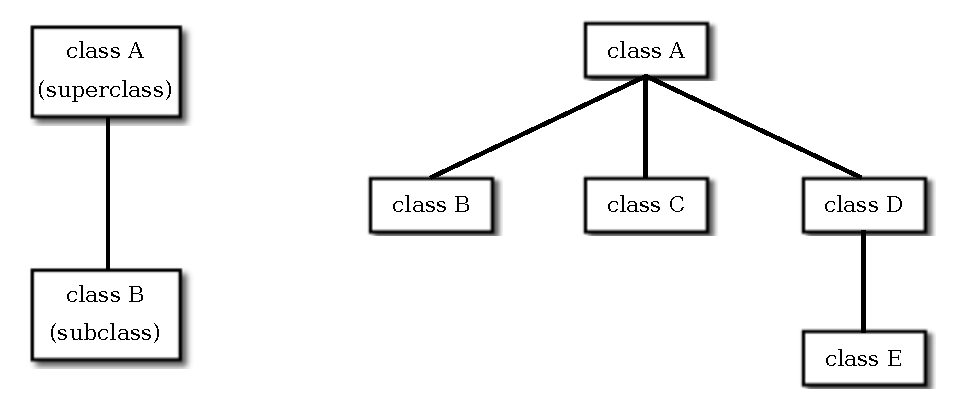
\includegraphics[scale=0.6]{images/subclass-superclass.eps}
}



In Java, to create a class named ``B" as a subclass of a class named ``A", 
you would write

\displaycode{class B extends A \{
    .
    .  // additions to, and modifications of,
    .  // stuff inherited from class A
    .
\}}\donedisplaycode

   


Several classes
can be declared as subclasses of the same superclass. The subclasses, which
might be referred to as ``sibling classes," share some structures and behaviors---namely, 
the ones they inherit from their common superclass. The superclass
expresses these shared structures and behaviors. In the diagram shown
on the right above,
classes B, C, and D are sibling classes. Inheritance can also extend over
several ``generations" of classes. This is shown in the diagram, where class E
is a subclass of class D which is itself a subclass of class A. In this case,
class E is considered to be a subclass of class A, even though it is not a
direct subclass.  This whole set of classes forms a small
\newword{class hierarchy}.





\subsection{Example: Vehicles}\label{OOP.5.3}



Let's look at
an example. Suppose that a program has to deal with motor vehicles, including
cars, trucks, and motorcycles. (This might be a program used by a Department of
Motor Vehicles to keep track of registrations.) The program could use a class
named \classname{Vehicle} to represent all types of vehicles.  Since cars, trucks,
and motorcycles are types of vehicles, they would be represented by subclasses
of the \classname{Vehicle} class, as shown in this class hierarchy diagram:


\par\dumpfigure{
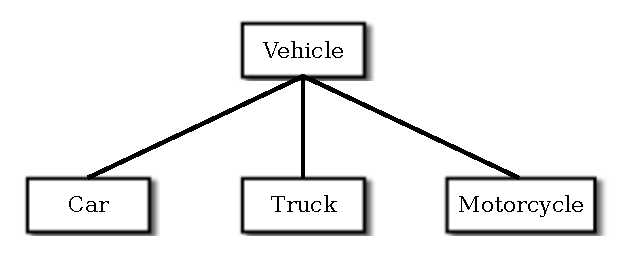
\includegraphics[scale=0.6]{images/vehicle-hierarchy.eps}
}
 
   
\noindent The \classname{Vehicle}
class would include instance variables such as \code{registrationNumber} and
\code{owner} and instance methods such as \code{transferOwnership()}. These
are variables and methods common to all vehicles. The three subclasses of
\classname{Vehicle}---\classname{Car}, 
\classname{Truck}, and \classname{Motorcycle}---could
then be used to hold variables and methods specific to particular types
of vehicles. The \classname{Car} class might add an instance variable
\code{numberOfDoors}, the \classname{Truck} class might have
\code{numberOfAxles}, and the \classname{Motorcycle} class could have a boolean
variable \code{hasSidecar}. (Well, it \underline{could} in theory at least, even
if it might give a chuckle to the people at the Department of Motor Vehicles.)
The declarations of these classes in a Java program would look, in outline, like
this (although they are likely to be  defined
in separate files and declared as \code{public} classes):

\displaycode{class Vehicle \{
   int registrationNumber;
   Person owner;  // (Assuming that a Person class has been defined!)
   void transferOwnership(Person newOwner) \{
       . . .
   \}
   . . .
\}

class Car extends Vehicle \{
   int numberOfDoors;
   . . .
\}

class Truck extends Vehicle \{
   int numberOfAxles;
   . . .
\}

class Motorcycle extends Vehicle \{
   boolean hasSidecar;
   . . .
\}}\donedisplaycode



Suppose that \code{myCar} is a variable of type \classname{Car} that has been
declared and initialized with the statement

\displaycode{Car myCar = new Car();}\donedisplaycode


\noindent Given this declaration, a program could refer to
\code{myCar.numberOfDoors}, since \code{numberOfDoors} is an instance
variable in the class \code{Car}. But since class \classname{Car} extends class
\classname{Vehicle}, a car also has all the structure and behavior of a vehicle.
This means that \code{myCar.registrationNumber}, \code{myCar.owner}, and
\code{myCar.transferOwnership()} also exist.


Now, in the real world, cars, trucks, and motorcycles are in fact vehicles.
The same is true in a program. That is, an object of type \classname{Car} or
\classname{Truck} or \classname{Motorcycle} is automatically an object of type
\classname{Vehicle} too. This brings us to the following Important Fact:

\par
\begin{center}

\textbf{A variable that can hold a reference\\
to an object of class A can also hold a reference\\
to an object belonging to any subclass of A.}

\end{center}


\noindent The practical effect of this in our example is that an object of type
\classname{Car} can be assigned to a variable of type \classname{Vehicle}. That is,
it would be legal to say

\displaycode{Vehicle myVehicle = myCar;}\donedisplaycode


\noindent or even

\displaycode{Vehicle myVehicle = new Car();}\donedisplaycode


\noindent After either of these statements, the variable \code{myVehicle} holds a
reference to a \classname{Vehicle} object that happens to be an instance of the
subclass, \classname{Car}. The object ``remembers" that it is in fact a
\classname{Car}, and not \textbf{just} a \classname{Vehicle}. Information about the
actual class of an object is stored as part of that object. It is even possible
to test whether a given object belongs to a given class, using the
\code{instanceof} operator. The test:

\displaycode{if (myVehicle instanceof Car) ...}\donedisplaycode


\noindent determines whether the object referred to by \code{myVehicle} is in fact a
car.


On the other hand, the assignment statement

\displaycode{myCar = myVehicle;}\donedisplaycode


\noindent would be illegal because \code{myVehicle} could potentially refer to other
types of vehicles that are not cars. This is similar to a problem we saw
previously in Subsection~\ref{basics.5.6}: The computer will not
allow you to assign an \ptype{int} value to a variable of type \ptype{short},
because not every \ptype{int} is a \ptype{short}. Similarly, it will not
allow you to assign a value of type \classname{Vehicle} to a variable of type
\classname{Car} because not every vehicle is a car. As in the case of
\ptype{ints} and \ptype{shorts}, the solution here is to use type-casting.
If, for some reason, you happen to know that \code{myVehicle} does in fact
refer to a \classname{Car}, you can use the type cast \code{(Car)myVehicle} to
tell the computer to treat \code{myVehicle} as if it were actually of type
\classname{Car}. So, you could say

\displaycode{myCar = (Car)myVehicle;}\donedisplaycode


\noindent and you could even refer to \code{((Car)myVehicle).numberOfDoors}. 
(The parentheses are necessary because of precedence.  The ``\code{.}"
has higher precedence than the type-cast, so
\code{(Car)myVehicle.numberOfDoors} would be read as \code{(Car)(myVehicle.numberOfDoors)},
an attempt to type-cast the \ptype{int}
\code{myVehicle.numberOfDoors} into a \classname{Vehicle},
which is impossible.)



As an
example of how this could be used in a program, suppose that you want to print
out relevant data about the \classname{Vehicle} referred to by
\code{myVehicle}.  If it's a \classname{car}, you will want
to print out the car's \code{numberOfDoors}, but you can't
say \code{myVehicle.numberOfDoors}, since there is no \code{numberOfDoors}
in the \classname{Vehicle} class.  But you could say:

\displaycode{System.out.println("Vehicle Data:");
System.out.println("Registration number:  " 
                              + myVehicle.registrationNumber);
if (myVehicle instanceof Car) \{
   System.out.println("Type of vehicle:  Car");
   Car c;
   c = (Car)myVehicle;  // Type-cast to get access to numberOfDoors!
   System.out.println("Number of doors:  " + c.numberOfDoors);
\}
else if (myVehicle instanceof Truck) \{
   System.out.println("Type of vehicle:  Truck");
   Truck t;
   t = (Truck)myVehicle;  // Type-cast to get access to numberOfAxles!
   System.out.println("Number of axles:  " + t.numberOfAxles);
\}
else if (myVehicle instanceof Motorcycle) \{
   System.out.println("Type of vehicle:  Motorcycle");
   Motorcycle m;
   m = (Motorcycle)myVehicle;  // Type-cast to get access to hasSidecar!
   System.out.println("Has a sidecar:    " + m.hasSidecar);
\}}\donedisplaycode



Note that for object types, when the computer executes a program, it checks
whether type-casts are valid. So, for example, if \code{myVehicle} refers to
an object of type \classname{Truck}, then the type cast \code{(Car)myVehicle}
would be an error.  When this happens, an exception of type
\classname{ClassCastException} is thrown.  This check is done at run time,
not compile time, because the actual type of the object referred to by \code{myVehicle}
is not known when the program is compiled.



\subsection{Polymorphism}\label{OOP.5.4}




As another example, consider a program that deals with shapes drawn on the
screen. Let's say that the shapes include rectangles, ovals, and roundrects of
various colors.  (A ``roundrect" is just a rectangle with rounded corners.)


\par\dumpfigure{
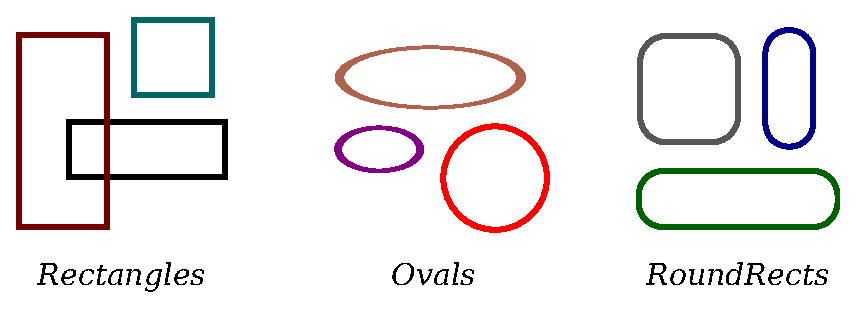
\includegraphics[scale=0.6]{images/various-shapes.eps}
}



Three classes, \classname{Rectangle}, \classname{Oval}, 
and \classname{RoundRect},
could be used to represent the three types of shapes. These three classes would
have a common superclass, \classname{Shape}, to represent features that all three
shapes have in common. The \classname{Shape} class could include instance
variables to represent the color, position, and size of a shape, and it could
include instance methods for changing the values of those properties.
Changing the color, for example, might involve changing the value of an
instance variable, and then redrawing the shape in its new color:

\displaycode{class Shape \{

    Color color; // (must be imported from package java.awt)
                   
    void setColor(Color newColor) \{
          // Method to change the color of the shape.
       color = newColor; // change value of instance variable
       redraw(); // redraw shape, which will appear in new color
    \}
    
    void redraw() \{
          // method for drawing the shape
       ? ? ?  // what commands should go here?
    \}

    . . .          // more instance variables and methods
 
\} // end of class Shape}\donedisplaycode



Now, you might see a problem here with the method \code{redraw()}. The
problem is that each different type of shape is drawn differently. The method
\code{setColor()} can be called for any type of shape. How does the computer
know which shape to draw when it executes the \code{redraw()}? Informally, we
can answer the question like this: The computer executes \code{redraw()} by
asking the shape to redraw \textbf{itself}. Every shape object knows
what it has to do to redraw itself.


In practice, this means that each of the specific shape classes has its own
\code{redraw()} method:

\displaycode{class Rectangle extends Shape \{
   void redraw() \{
      . . .  // commands for drawing a rectangle
   \}
   . . . // possibly, more methods and variables
\}

class Oval extends Shape \{
   void redraw() \{
      . . .  // commands for drawing an oval
   \}
   . . . // possibly, more methods and variables
\}

class RoundRect extends Shape \{
   void redraw() \{
      . . .  // commands for drawing a rounded rectangle
   \}
   . . . // possibly, more methods and variables
\}}\donedisplaycode



Suppose that \code{someShape} is a variable of type \classname{Shape}.   
Then it could refer to
an object of any of the types \classname{Rectangle}, \classname{Oval}, or
\classname{RoundRect}. As a program executes, and the value of \code{someShape}
changes, it could even refer to objects of different types at different times!
Whenever the statement

\displaycode{someShape.redraw();}\donedisplaycode


\noindent is executed, the redraw method that is actually called is the one
appropriate for the type of object to which \code{someShape} actually refers.
There may be no way of telling, from looking at the text of the program, what
shape this statement will draw, since it depends on the value that
\code{someShape} happens to have when the program is executed. Even more is
true. Suppose the statement is in a loop and gets executed many times. If the
value of \code{someShape} changes as the loop is executed, it is possible that
the very same statement ``\code{someShape.redraw();}" will call different
methods and draw different shapes as it is executed over and over. We say that
the \code{redraw()} method is \newword{polymorphic}. A
method is polymorphic if the action performed by the method depends on the
actual type of the object to which the method is applied. Polymorphism is one
of the major distinguishing features of object-oriented programming.  This can be
seen most vividly, perhaps, if we have an array of shapes.  Suppose that
\code{shapelist} is an a variable of type \atype{Shape\hbox{[\hskip2pt]}},
and that the array has already been created and filled with data.  Some of
the elements in the array might be \classname{Rectangles},
some might be \classname{Ovals}, and some might be \classname{RoundRects}.
We can draw all the shapes in the array by saying

\displaycode{for (int i = 0; i \< shapelist.length; i++ ) \{
    Shape shape = shapelist[i];
    shape.redraw();
\}}\donedisplaycode


\noindent As the computer goes through this loop, the statement \code{shape.redraw()}
will sometimes draw a rectangle, sometimes an oval, and sometimes a roundrect,
depending on the type of object to which array element number \code{i} refers.


Perhaps this becomes more understandable if we change our terminology a bit:
In object-oriented programming, calling a method is often referred to as
sending a \newword{message} to an object. The object
responds to the message by executing the appropriate method. The statement
``\code{someShape.redraw();}" is a message to the object referred to by
\code{someShape}. Since that object knows what type of object it is, it knows
how it should respond to the message. From this point of view, the computer
always executes ``\code{someShape.redraw();}" in the same way: by sending a
message. The response to the message depends, naturally, on who receives it.
From this point of view, objects are active entities that send and receive
messages, and polymorphism is a natural, even necessary, part of this view.
Polymorphism just means that different objects can respond to the same message
in different ways.


 One of the
most beautiful things about polymorphism is that it lets code that you write do
things that you didn't even conceive of, at the time you wrote it. Suppose that
I decide to add beveled rectangles to the types of shapes my program can deal
with.  A beveled rectangle has a triangle cut off each corner:
   

\par\dumpfigure{
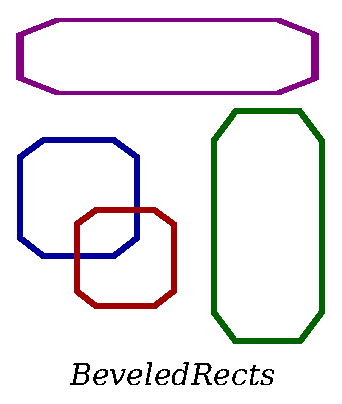
\includegraphics[scale=0.6]{images/beveled-rects.eps}
}


   

To implement beveled rectangles, I can write a new subclass, \classname{BeveledRect}, of
class \classname{Shape} and give it its own \code{redraw()} method.
Automatically, code that I wrote previously---such as the statement
\code{someShape.redraw()}---can now suddenly start drawing beveled
rectangles, even though the beveled rectangle class didn't exist when I wrote
the statement!


\mybreak



In the statement ``\code{someShape.redraw();}", the \code{redraw} message
is sent to the object \code{someShape}. Look back at the method in the
\classname{Shape} class for changing the color of a shape:

\displaycode{void setColor(Color newColor) \{
   color = newColor; // change value of instance variable
   redraw(); // redraw shape, which will appear in new color
\}}\donedisplaycode


\noindent A \code{redraw} message is sent here, but which object is it sent to?
Well, the \code{setColor} method is itself a message that was sent to some
object. The answer is that the \code{redraw} message is sent to that \textbf{same
object}, the one that received the \code{setColor} message. If that object is
a rectangle, then it contains a \code{redraw()} method for drawing rectangles,
and that is the one that is executed.  If the object is an oval, then it is
the \code{redraw()} method from the \classname{Oval} class. This is what you
should expect, but it means that the ``\code{redraw();}" statement in the
\code{setColor()} method does \textbf{not} necessarily call the
\code{redraw()} method in the \classname{Shape} class! The \code{redraw()}
method that is executed could be in any subclass of \classname{Shape}.
This is just another case of polymorphism.




\subsection{Abstract Classes}\label{OOP.5.5}



Whenever a \classname{Rectangle}, \classname{Oval}, 
or \classname{RoundRect} object
has to draw itself, it is the \code{redraw()} method in the appropriate class
that is executed. This leaves open the question, What does the
\code{redraw()} method in the \classname{Shape} class do? How should it be
defined?


The answer may be surprising: We should leave it blank! The fact is that the
class \classname{Shape} represents the abstract idea of a shape, and there is no
way to draw such a thing. Only particular, concrete shapes like rectangles and
ovals can be drawn. So, why should there even be a \code{redraw()} method in
the \classname{Shape} class? Well, it has to be there, or it would be illegal to
call it in the \code{setColor()} method of the \classname{Shape} class, and it
would be illegal to write ``\code{someShape.redraw()};". The compiler would
complain that \code{someShape} is a variable of type \classname{Shape} and
there's no \code{redraw()} method in the \classname{Shape} class.


Nevertheless the version of \code{redraw()} in the \classname{Shape} class itself
will never actually be called. In fact, if you think about it, there can never be any
reason to construct an actual object of type \classname{Shape}! You can have
\textbf{variables} of type \classname{Shape}, but the objects they refer
to will always belong to one of the subclasses of \classname{Shape}. We say that
\classname{Shape} is an \newword{abstract class}. An abstract
class is one that is not used to construct objects, but only as a basis for
making subclasses. An abstract class exists \textbf{only} to express
the common properties of all its subclasses.  A class that is not abstract
is said to be \newword{concrete}.  You can create objects belonging to
a concrete class, but not to an abstract class.  A variable whose type is given
by an abstract class can only refer to objects that belong to concrete subclasses
of the abstract class.


Similarly, we say that the \code{redraw()} method in class \classname{Shape}
is an \newword{abstract method}, since it is never meant to
be called. In fact, there is nothing for it to do---any actual redrawing is
done by \code{redraw()} methods in the subclasses of \classname{Shape}. The
\code{redraw()} method in \classname{Shape} has to be there. But it is there
only to tell the computer that \textbf{all} \code{Shapes} understand the
\code{redraw} message. As an abstract method, it exists merely to specify the
common interface of all the actual, concrete versions of \code{redraw()} in
the subclasses. There is no reason for the abstract
\code{redraw()} in class \classname{Shape} to contain any code at all.


\classname{Shape} and its \code{redraw()} method are semantically abstract.
You can also tell the computer, syntactically, that they are abstract by adding
the modifier ``\code{abstract}" to their definitions. For an abstract method,
the block of code that gives the implementation of an ordinary method is
replaced by a semicolon. An implementation must then be provided for the abstract
method in any concrete subclass of the abstract class. Here's what the
\classname{Shape} class would look like as an abstract class:

\displaycode{public abstract class Shape \{

    Color color;   // color of shape. 
                              
    void setColor(Color newColor) \{
          // method to change the color of the shape
       color = newColor; // change value of instance variable
       redraw(); // redraw shape, which will appear in new color
    \}
    
    abstract void redraw();
          // abstract method---must be defined in 
          // concrete subclasses

    . . .  // more instance variables and methods

\} // end of class Shape}\donedisplaycode



Once you have declared the class to be \code{abstract}, it becomes illegal to try to create actual objects
of type \classname{Shape}, and the computer will report a syntax error if you try to do
so.


Note, by the way, that the \classname{Vehicle} class discussed above would probably
also be an abstract class.  There is no way to own a vehicle as such---the actual vehicle has
to be a car or a truck or a motorcycle, or some other ``concrete" type of vehicle.


\mybreak
   


Recall from Subsection~\ref{OOP.3.3} that a class that is not explicitly declared to be a subclass
of some other class is automatically made a subclass of the standard class \classname{Object}.
That is, a class declaration with no ``\code{extends}" part such as

\displaycode{public class myClass \{ . . .}\donedisplaycode


\noindent is exactly equivalent to

\displaycode{public class myClass extends Object \{ . . .}\donedisplaycode



This means that class \classname{Object} is at the top of a huge class hierarchy that
includes every other class.  (Semantically, \classname{Object} is an abstract class, in fact
the most abstract class of all.  Curiously, however, it is not declared to be \code{abstract}
syntactically, which means that you can create objects of type \classname{Object}.  
However, there is not much that you can do with them.)


Since every class is a subclass of \classname{Object}, a variable of type
\classname{Object} can refer to any object whatsoever, of any type.  
Similarly, an array of
type \atype{Object\hbox{[\hskip2pt]}} can hold objects of any type. 


\mybreak



The sample source code file \sourceref{ShapeDraw.java} uses an abstract
\classname{Shape} class and an array of type \atype{Shape\hbox{[\hskip2pt]}}
to hold a list of shapes. 
You might want to look at this file, even though you won't be able to
understand all of it at this time. Even the definitions of the shape classes
are somewhat different from those that I have described in this section. (For example,
the \code{draw()} method has a parameter of type
\classname{Graphics}. This parameter is required because drawing in 
Java requires a graphics context.) I'll return to similar examples in later chapters when you know more
about GUI programming. However, it would still be worthwhile to look at the definition
of the \classname{Shape} class and its subclasses in the source code.
You might also check how an array is used to hold the list of shapes.  Here is a screenshot
from the program:
 
 
\par\dumpfigure{
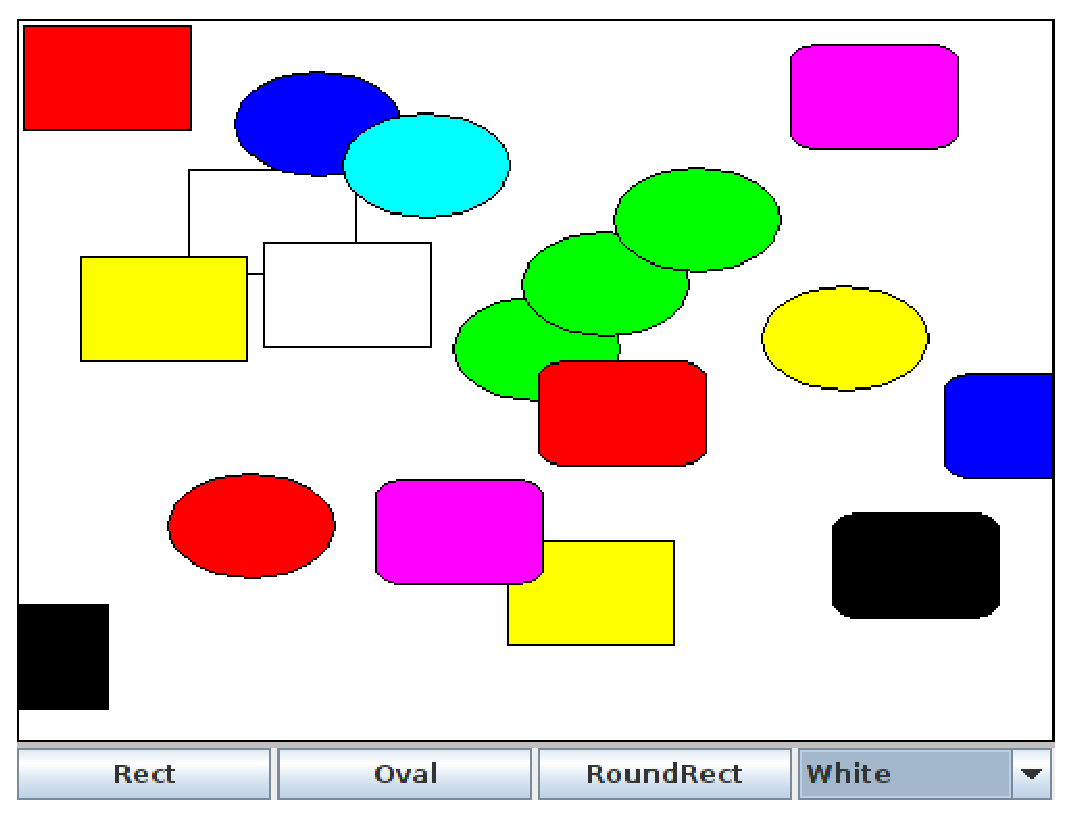
\includegraphics[scale=0.5]{images/shapedraw-screenshot.eps}
}

   

If you run the \code{ShapeDraw} program, 
you can click one of the buttons along the bottom to add a shape to the picture.
The new shape will appear in the upper left corner of the drawing area. The color
of the shape is given by the ``pop-up menu" in the lower right. Once a shape is
on the screen, you can drag it around with the mouse. A shape will maintain the
same front-to-back order with respect to other shapes on the screen, even while
you are dragging it. However, you can move a shape out in front of all the
other shapes if you hold down the shift key as you click on it.
   

In the program, the only time when the actual class of a shape is used is
when that shape is added to the screen. Once the shape has been created, it is
manipulated entirely as an abstract shape. The routine that implements
dragging, for example, works with variables of type \classname{Shape} and
makes no reference to any of its subclasses. As the
shape is being dragged, the dragging routine just calls the
shape's draw method each time the shape has to be drawn, so it doesn't
have to know how to draw the shape or even what type of shape it is. The object
is responsible for drawing itself. If I wanted to add a new type of shape to
the program, I would define a new subclass of \classname{Shape}, add another
button, and program the button to add the correct type of shape
to the screen. No other changes in the programming would be necessary.





   



\section{this and super}\label{OOP.6}

   

\start{{\Large A}lthough the basic ideas} of object-oriented
programming are reasonably simple and clear, they are subtle, and they take
time to get used to. And unfortunately, beyond the basic ideas there are a lot
of details. The rest of this chapter covers more of those
annoying details. Remember that you don't need to master everything in
this chapter the first time through.  In this
section, we'll look at two variables, \code{this} and \code{super}, that are
automatically defined in any instance method.

\subsection{The Special Variable this}\label{OOP.6.1}



What does it mean when you use a simple identifier such as \code{amount}
or \code{process()} to refer to a variable or method?  The answer depends
on scope rules that tell where and how each declared variable and method can
be accessed in a program.  Inside the definition of a method, a simple variable name might
refer to a local variable or parameter, if there is one ``in scope," that is, one
whose declaration is in effect at the point in the source code where the reference
occurs.  If not, it must refer to a member variable of the class in which the
reference occurs.  Similarly, a simple method name must refer to a method in 
the same class.


A \textbf{static} member of a class has a simple name that can only be used inside
the class definition; for use outside the class, it has a full name of the form
\bnf{class-name}.\bnf{simple-name}. For example, ``\code{Math.PI}" is a static
member variable with simple name ``\code{PI}" in the class ``\classname{Math}".
It's always legal to use the full name of a static member, even within the
class where it's defined. Sometimes it's even necessary, as when the simple
name of a static member variable is hidden by a local variable or parameter of the same
name.


Instance variables and instance methods also have simple names. The simple
name of such an instance member can be used in instance methods in the class
where the instance member is defined (but not in static methods).
Instance members also have full names---but remember that an instance variable
or instance method is actually contained in an object rather than in a class, and each object has its
own version.  A full name of an instance member starts with a
reference to the object that contains the instance member.  For example,
if \code{std} is a variable that refers to an object of type \classname{Student},
then \code{std.test1} could be a full name for an instance variable named
\code{test1} that is contained in that object.


But when we are working inside a class and use a simple name to refer to an instance variable
like \code{test1}, where is the object that contains the variable?
The solution to this riddle is simple: Suppose that a reference to ``\code{test1}"
occurs in the definition of some instance method.  The actual method that
gets executed is part of some particular object of
type \classname{Student}.   When that method gets executed, the
occurrence of the name ``\code{test1}" refers to the \code{test1} variable
\textbf{in that same object}.  (This is why simple names of instance members cannot
be used in static methods---when a static method is executed, it is not part
of an object, and hence there are no instance members in sight!)


This leaves open the question of full names for instance members inside the
same class where they are defined.  We need a way to refer to ``the object that
contains this method."  Java defines a special variable named \newword{this}
for just this purpose.  The variable \code{this} can be used in the source
code of an instance method to refer to the object that contains the method.
This intent of the name, ``\code{this}," is to refer to ``this object," the one
right here that this very method is in.  If \code{var} is an instance variable
in the same object as the method, then ``\code{this.var}" is a full name for that
variable. If \code{otherMethod()} is an instance method in the same object,
then \code{this.otherMethod()} could be used to call that method. Whenever
the computer executes an instance method, it automatically sets the variable
\code{this} to refer to the object that contains the method.


(Some object oriented languages use the name ``self" instead of ``this."  Here, an
object is seen as an entity that receives messages and responds by performing some
action.  From the point of view of that entity, an instance variable such as
\code{self.name} refers to the entity's own \code{name}, something
that is part of the entity itself.  Calling an instance method such as 
\code{self.redraw()} is like saying ``message to self: redraw!")


One common use of \code{this} is in constructors. For example:

\displaycode{public class Student \{

    private String name;  // Name of the student.
    
    public Student(String name) \{
         // Constructor.  Create a student with specified name.
       this.name = name;
    \}
      .
      .   // More variables and methods.
      .
\}}\donedisplaycode


\noindent In the constructor, the instance variable called \code{name} is hidden by
a formal parameter that is also called ``name." 
However, the instance variable can still be referred to by
its full name, which is \code{this.name}. In the assignment statement 
``\code{this.name~=~name}", the value of
the formal parameter, \code{name}, is assigned to the instance variable,
\code{this.name}. This is considered to be acceptable style: There is no need
to dream up cute new names for formal parameters that are just used to
initialize instance variables. You can use the same name for the parameter as
for the instance variable.


There are other uses for \code{this}.  Sometimes, when you are writing an
instance method, you need to pass the object that contains the method to a
subroutine, as an actual parameter. In that case, you can use \code{this} as
the actual parameter. For example, if you wanted to print out a string
representation of the object, you could say
``\code{System.out.println(this);}".  Or you could assign the value of
\code{this} to another variable in an assignment statement.  You can store
it in an array.  In fact, you can
do anything with \code{this} that you could do with any other variable,
except change its value. (Consider it to be a \code{final} variable.)


   
\subsection{The Special Variable super}\label{OOP.6.2}



Java also defines another special variable, named ``\code{super}", for use
in the definitions of instance methods. The variable \code{super} is for use
in a subclass. Like \code{this}, \code{super} refers to the object that
contains the method. But it's forgetful. It forgets that the object belongs to
the class you are writing, and it remembers only that it belongs to the
superclass of that class. The point is that the class can contain additions and
modifications to the superclass. \code{super} doesn't know about any of those
additions and modifications; it can only be used to refer to methods and
variables in the superclass.


Let's say that the class that you are writing contains an instance method
named \code{doSomething()}. Consider the subroutine call statement
\code{super.doSomething()}. Now, \code{super} doesn't know anything about
the \code{doSomething()} method in the subclass. It only knows about things
in the superclass, so it tries to execute a method named \code{doSomething()}
from the superclass. If there is none---if the \code{doSomething()} method
was an addition rather than a modification---you'll get a syntax error.


The reason \code{super} exists is so you can get access to things in the
superclass that are \textbf{hidden} by things in the subclass. For example,
\code{super.var} always refers to an instance variable named \code{var} in the
superclass. This can be useful for the following reason: If a class contains an
instance variable with the same name as an instance variable in its superclass,
then an object of that class will actually contain two variables with the same
name: one defined as part of the class itself and one defined as part of the
superclass. The variable in the subclass does not \textbf{replace} the
variable of the same name in the superclass; it merely \textbf{hides}
it. The variable from the superclass can still be accessed, using
\code{super}.


When a subclass contains an instance method that has the same signature as a
method in its superclass, the method from the superclass is hidden in the same
way. We say that the method in the subclass \newword{overrides} 
the method from the superclass. Again, however,
\code{super} can be used to access the method from the superclass.


The major use of \code{super} is to override a method with a new method
that \textbf{extends} the behavior of the inherited method, instead of
\textbf{replacing} that behavior entirely. The new method can use
\code{super} to call the method from the superclass, and then it can add
additional code to provide additional behavior. As an example, suppose you have
a \classname{PairOfDice} class that includes a \code{roll()} method. Suppose
that you want a subclass, \classname{GraphicalDice}, to represent a pair of dice
drawn on the computer screen. The \code{roll()} method in the
\classname{GraphicalDice} class should do everything that the \code{roll()}
method in the \classname{PairOfDice} class does. We can express this with a call
to \code{super.roll()}, which calls the method in the superclass. 
But in addition to that, the \code{roll()} method
for a \classname{GraphicalDice} object has to redraw the dice to show the new
values. The \classname{GraphicalDice} class might look something like this:

\displaycode{public class GraphicalDice extends PairOfDice \{

    public void roll() \{
            // Roll the dice, and redraw them.
         super.roll();  // Call the roll method from PairOfDice.
         redraw();      // Call a method to draw the dice.
    \}
       .
       .  // More stuff, including definition of redraw().
       .
\}}\donedisplaycode


\noindent Note that this allows you to extend the behavior of the \code{roll()}
method even if you don't know how the method is implemented in the
superclass!
   


\subsection{super and this As Constructors}\label{OOP.6.3}



Constructors are not inherited. That is, if you extend an existing class to
make a subclass, the constructors in the superclass do \code{not} become part
of the subclass. If you want constructors in the subclass, you have to define
new ones from scratch. If you don't define any constructors in the subclass,
then the computer will make up a default constructor, with no parameters, for
you.


This could be a problem, if there is a constructor in the superclass that
does a lot of necessary work. It looks like you might have to repeat all that
work in the subclass! This could be a \textbf{real} problem if you
don't have the source code to the superclass, and don't even know how it is implemented.  
It might look like an impossible problem, if 
the constructor in the superclass uses \code{private} member
variables that you don't even have access to in the subclass!


Obviously, there has to be some fix for this, and there is. It involves the
special variable, \code{super}. As the very first statement in a constructor,
you can use \code{super} to call a constructor from the superclass. The
notation for this is a bit ugly and misleading, and it can only be used in this
one particular circumstance: It looks like you are calling \code{super} as a
subroutine (even though \code{super} is not a subroutine and you can't call
constructors the same way you call other subroutines anyway). As an example,
assume that the \classname{PairOfDice} class has a constructor that takes two
integers as parameters. Consider a subclass:

\displaycode{public class GraphicalDice extends PairOfDice \{

     public GraphicalDice() \{  // Constructor for this class.
     
         super(3,4);  // Call the constructor from the
                      //   PairOfDice class, with parameters 3, 4.
                      
         initializeGraphics();  // Do some initialization specific
                                //   to the GraphicalDice class.
     \}
        .
        .  // More constructors, methods, variables...
        .
\}}\donedisplaycode



The statement ``\code{super(3,4);}" calls the constructor from
the superclass.  This call must be the first line of the constructor in the
subclass.  Note that if you don't explicitly call a constructor from the
superclass in this way, then the default constructor from the superclass, the one with
no parameters, will be called automatically.  (And if no such constructor exists
in the superclass, the compiler will consider it to be a syntax error.)
   

You can use the special variable \code{this} in
exactly the same way to call another constructor in the same class.
That is, the very first line of a constructor can look like a subroutine
call with ``this" as the name of the subroutine.  The result is that the
body of another constructor in the same class is executed.
This can be very useful since it can save you from repeating the 
same code in several different constructors.  As an example, consider
\sourceref{MosaicPanel.java}, which was used indirectly
in Section~\ref{subroutines.6}.  A \classname{MosaicPanel}
represents a grid of colored rectangles.  It has a constructor with many 
parameters:

\displaycode{public MosaicPanel(int rows, int columns, 
                 int preferredBlockWidth, int preferredBlockHeight, 
                 Color borderColor, int borderWidth)}\donedisplaycode
   

\noindent This constructor provides a lot of options and does a lot of initialization.
I wanted to provide easier-to-use
constructors with fewer options, but all the initialization still has
to be done.  The class also contains these constructors:

\displaycode{public MosaicPanel() \{
    this(42,42,16,16);
\}

public MosaicPanel(int rows, int columns) \{
    this(rows,columns,16,16);
\}

public MosaicPanel(int rows, int columns, 
                   int preferredBlockWidth, int preferredBlockHeight) \{
    this(rows, columns, preferredBlockWidth, preferredBlockHeight, null, 0);
\}}\donedisplaycode


\noindent Each of these constructors exists just to call another constructor, while providing
constant values for some of the parameters.  For example,
\code{this(42,42,16,16)} calls the last constructor listed here,
while that constructor in turn calls the main, six-parameter constructor.  That main constructor
is eventually called in all cases, so that all the essential initialization gets done
in every case.




   



\section{Interfaces}\label{OOP.7}




Some object-oriented programming languages, such as C++, allow a class to
extend two or more superclasses. This is called \newword{multiple inheritance}. 
In the illustration below, for example, class~E is shown as
having both class~A and class~B as direct superclasses, while class~F has three
direct superclasses.


\par\dumpfigure{
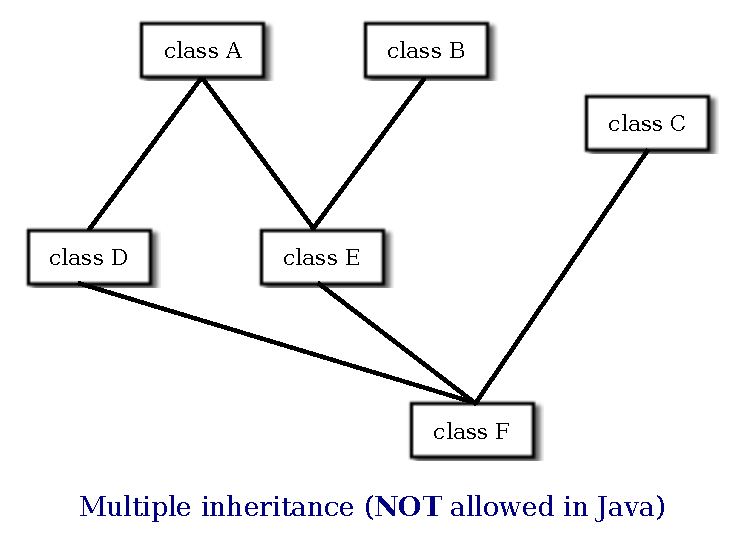
\includegraphics[scale=0.6]{images/multiple-inheritance.eps}
}

   

Such multiple inheritance is \textbf{not} allowed in Java. The
designers of Java wanted to keep the language reasonably simple, and felt that
the benefits of multiple inheritance were not worth the cost in increased
complexity. However, Java does have a feature that can be used to accomplish
many of the same goals as multiple inheritance: \newword{interfaces}.


\subsection{Defining and Implementing Interfaces}\label{OOP.7.1}




We've encountered the term ``interface" before, in connection with black
boxes in general and subroutines in particular. The interface of a subroutine
consists of the name of the subroutine, its return type, and the number and
types of its parameters. This is the information you need to know if you want
to call the subroutine. A subroutine also has an implementation: the block of
code which defines it and which is executed when the subroutine is called.


In Java, \code{interface} is a reserved word with an additional, technical
meaning. An ``\code{interface}" in this sense consists of a set of instance method
interfaces, without any associated implementations.  (Actually, a Java interface
can contain other things as well, as we'll see later.)
A class can \newword{implement} 
an \code{interface} by providing an implementation
for each of the methods specified by the interface. Here is an example of a
very simple Java \code{interface}:

\displaycode{public interface Drawable \{
   public void draw(Graphics g);
\}}\donedisplaycode


\noindent This looks much like a class definition, except that the implementation of
the \code{draw()} method is omitted. A class that implements the
\code{interface} \classname{Drawable} must provide an implementation for this
method. Of course, the class can also include other methods and variables. For
example,

\displaycode{public class Line implements Drawable \{
    public void draw(Graphics g) \{
        . . . // do something---presumably, draw a line
    \}
    . . . // other methods and variables
\}}\donedisplaycode


\noindent Note that to implement an interface, a class must do more than simply provide
an implementation for each method in the interface; it must also \textbf{state} that
it implements the interface, using the reserved word \code{implements} as
in this example: ``\code{public class Line \textbf{implements} Drawable}".
Any concrete class that implements the \classname{Drawable} interface must defines a
\code{draw()} instance method. Any object created from such a class includes
a \code{draw()} method. We say that an \textbf{object} implements an
\code{interface} if it belongs to a class that implements the interface. For
example, any object of type \classname{Line} implements the \classname{Drawable}
interface.


While a class can \textbf{extend} only one other class, it can
\textbf{implement} any number of interfaces. In fact, a class can both extend
one other class and implement one or more interfaces.  So, we can have things
like

\displaycode{class FilledCircle extends Circle 
                        implements Drawable, Fillable \{
   . . .
\}}\donedisplaycode



The point of all this is that, although interfaces are not classes, they are
something very similar. An interface is very much like an abstract class, that
is, a class that can never be used for constructing objects, but can be used as
a basis for making subclasses. The subroutines in an interface are abstract
methods, which must be implemented in any concrete class that implements the
interface.  You can compare the \classname{Drawable}
interface with the abstract class

\displaycode{public abstract class AbstractDrawable \{
   public abstract void draw(Graphics g);
\}}\donedisplaycode


\noindent The main difference is that a class that extends \classname{AbstractDrawable}
cannot extend any other class, while a class that implements \classname{Drawable}
can also extend some class, as well as implement other interfaces.  Of course, an
abstract class can contain non-abstract methods as well as abstract methods.
An interface is like a ``pure" abstract class, which contains only abstract methods.


Note that the methods declared in an interface must be \code{public}.  In fact,
since that is the only option, it is not necessary to specify the access modifier in
the declaration.


In addition to method declarations, an interface can also include variable
declarations.  The variables must be \code{"public static final"}
and effectively become public static final variables in every class that implements
the interface.  In fact, since the variables can only be public and static and final,
specifying the modifiers is optional.  For example,

\displaycode{public interface ConversionFactors \{
    int INCHES\_PER\_FOOT = 12;
    int FEET\_PER\_YARD = 3;
    int YARDS\_PER\_MILE = 1760;
\}}\donedisplaycode


\noindent This is a convenient way to define named constants that can be
used in several classes.  A class that implements \classname{ConversionFactors}
can use the constants defined in the interface as if they were defined in the
class.


You are not likely to need to write your own interfaces until you get to the
point of writing fairly complex programs. However, there are several interfaces
that are used in important ways in Java's standard packages. You'll learn about
some of these standard interfaces in the next few chapters, and you will
write classes that implement them.




\subsection{Interfaces as Types}\label{OOP.7.2}



As with abstract classes, even though you can't construct an
object from an interface, you can declare a variable whose type is given by the
interface. For example, if \classname{Drawable} is the interface given above, and if
\classname{Line} and \classname{FilledCircle} are classes that implement
\classname{Drawable}, as above, then you could say:

\displaycode{Drawable figure;  // Declare a variable of type Drawable.  It can
                  //    refer to any object that implements the
                  //    Drawable interface.
                  
figure = new Line();  // figure now refers to an object of class Line
figure.draw(g);   // calls draw() method from class Line

figure = new FilledCircle();   // Now, figure refers to an object
                               //   of class FilledCircle.
figure.draw(g);   // calls draw() method from class FilledCircle}\donedisplaycode


\noindent A variable of type \classname{Drawable} can refer to any object of any class
that implements the \classname{Drawable} interface. A statement like
\code{figure.draw(g)}, above, is legal because \code{figure} is of type
\classname{Drawable}, and \textbf{any} 
\classname{Drawable} object has a \code{draw()}
method.  So, whatever object \code{figure} refers to, that object must
have a \code{draw()} method.


Note that a \newword{type} is something that can be used
to declare variables. A type can also be used to specify the type of a
parameter in a subroutine, or the return type of a function. In Java, a type
can be either a class, an interface, or one of the eight built-in primitive
types. These are the only possibilities. Of these, however, only classes can be
used to construct new objects.


An interface can also be the base type of an array.  For example, we can
use an array type \atype{Drawable\hbox{[\hskip2pt]}} to declare
variables and create arrays.  The elements
of the array can refer to any objects that implement the \classname{Drawable}
interface:

\displaycode{Drawable[] listOfFigures;
listOfFigures = new Drawable[10];
listOfFigures[0] = new Line();
listOfFigures[1] = new FilledCircle();
listOfFigures[2] = new Line();
  .
  .
  .}\donedisplaycode

  
  \noindent Every element of the array will then have a \code{draw()} method, so that
  we can say things like \code{listOfFigures[i].draw(g)}.



   
\subsection{Interfaces in Java 8}\label{OOP.7.3}



The newest version of Java, Java~8, makes a few useful additions to interfaces.
The one that I will discuss here is \newword{default methods}.  Unlike the usual
abstract methods in interfaces, a default method has an implementation.  When a class
implements the interface, it does not have to provide an implementation for the
default method---although it can do so if it wants to provide a different implementation.
Essentially, default methods are inherited from interfaces in much the same way that
ordinary methods are inherited from classes.  This moves Java partway towards supporting
multiple inheritance.  It's not true multiple inheritance, however, since interfaces
still cannot define instance variables.


A default method in an interface must be marked with the modifier \code{default}.
It can optionally be marked \code{public} but, as for everything else in interfaces,
default methods are automatically public and the \code{public} modifier can be omitted.
Here is an example.:

\displaycode{public interface Readable \{ // represents a source of input

    public char readChar();  // read the next character from the input

    default public String readLine() \{ // read up to the next line feed
        StringBuilder line = new StringBuilder();
        char ch = readChar();
        while (ch != '\1n') \{
            line.append(ch);
            ch = readChar();
        \}
        return line.toString();
    \}

\}}\donedisplaycode


\noindent A concrete class that implements this interface must provide an implementation for
\code{readChar()}.  It will inherit a definition for \code{readLine()} from the interface,
but can provide a new definition if necessary.    Note that the default
\code{readLine()} calls the abstract method \code{readChar()},
whose definition will only be provided in the implementing class.  The reference
to \code{readChar()} in the definition is polymorphic.
The default implementation of \code{readLine()} is one that would make 
sense in almost any class that implements \classname{Readable}.  Here's
a rather silly example of a class that implements \classname{Readable},
including a \code{main()} routine that tests the class. Can you figure out
what it does?


\displaycode{public class Stars implements Readable \{

    public char readChar() \{
        if (Math.random() \> 0.02)
           return '*';
        else
           return '\1n';
    \}
    
    public static void main(String[] args) \{
        Stars stars = new Stars();
        for (int i = 0 ; i \< 10; i++ ) \{
            String line = stars.readLine();
            System.out.println( line );
        \}
    \}
      
\}}\donedisplaycode



Default methods provide Java with a capability similar to something called
a ``mixin" in other programming languages, namely the ability to mix functionality from
another source into a class. Since a class can implement several interfaces,
it is possible to mix in functionality from several different sources.




   



\section{Nested Classes}\label{OOP.8}



\start{{\Large A} class seems like it should be} a pretty important thing. A class is a
high-level building block of a program, representing a potentially complex idea
and its associated data and behaviors. I've always felt a bit silly writing
tiny little classes that exist only to group a few scraps of data together.
However, such trivial classes are often useful and even essential. Fortunately,
in Java, I can ease the embarrassment, because one class can be nested inside
another class. My trivial little class doesn't have to stand on its own. It
becomes part of a larger more respectable class. This is particularly useful
when you want to create a little class specifically to support the work of a
larger class. And, more seriously, there are other good reasons for nesting the
definition of one class inside another class.


In Java, a \newword{nested class} is any class whose definition is inside the
definition of another class.  (In fact, a class can even be nested inside a subroutine,
which must, of course, itself be inside a class).
Nested classes can be either \newword{named} 
or \newword{anonymous}. I will come
back to the topic of anonymous classes later in this section.  A named nested
class, like most other things that occur in classes, can be either static or
non-static.
 
   
\subsection{Static Nested Classes}\label{OOP.8.1}


 

The definition of a static nested class looks just like the definition of any other class,
except that it is nested inside another class and it has the modifier \code{static}
as part of its declaration. A static nested class is part of the static structure of the
containing class. It can be used inside that class to create objects in the
usual way. If it is used
outside the containing class, its name
must indicate its membership in the containing class.  That is, the full name of
the static nested class consists of the name of the class in which it is nested, followed
by a period, followed by the name of the nested class.  This is similar to other
static components of a class: A static nested class is part of the class itself
in the same way that static member variables are parts of the class itself.


For example, suppose a class named \classname{WireFrameModel} represents a set
of lines in three-dimensional space. (Such models are used to represent
three-dimensional objects in graphics programs.) Suppose that the
\classname{WireFrameModel} class contains a static nested class, \classname{Line},
that represents a single line. Then, outside of the class
\classname{WireFrameModel}, the \classname{Line} class would be referred to as
\code{WireFrameModel.Line}. Of course, this just follows the normal naming
convention for static members of a class. The definition of the
\classname{WireFrameModel} class with its nested \classname{Line} class would look,
in outline, like this:

\displaycode{public class WireFrameModel \{

   . . . // other members of the WireFrameModel class
   
   static public class Line \{
         // Represents a line from the point (x1,y1,z1)
         // to the point (x2,y2,z2) in 3-dimensional space.
      double x1, y1, z1;
      double x2, y2, z2;
   \} // end class Line
   
   . . . // other members of the WireFrameModel class
   
\} // end WireFrameModel}\donedisplaycode


\noindent The full name of the nested class is \classname{WireFrameModel.Line}.
That name can be used, for example, to declare variables.
Inside the \classname{WireFrameModel} class, a \classname{Line} object would be
created with the constructor ``\code{new~Line()}". Outside the class, 
``\code{new~WireFrameModel.Line()}" would be used.


A static nested class has full access to the static members of the containing
class, even to the \code{private} members. Similarly, the containing class has full
access to the members of the nested class, even if they are marked \code{private}.  
This can be another motivation for
declaring a nested class, since it lets you give one class access to the
private members of another class without making those members generally
available to other classes.  Note also that a nested class can itself be private,
meaning that it can only be used inside the class in which it is nested.


When you compile the above class definition, two class files will be
created. Even though the definition of \classname{Line} is nested inside
\classname{WireFrameModel}, the compiled \classname{Line} class is stored in a
separate file. The name of the class file for \classname{Line} will be
\code{WireFrameModel\$Line.class}.



\subsection{Inner Classes}\label{OOP.8.2}



Non-static nested classes are referred to as \newword{inner classes}.
Inner classes are not, in practice, very different from static
nested classes, but a non-static nested class is actually associated with an
object rather than with the class in which its definition is nested. This can take some
getting used to.


Any non-static member of a class is not really part of the class itself
(although its source code is contained in the class definition). This is true
for inner classes, just as it is for any other non-static part of a
class. The non-static members of a class specify what will be contained in
objects that are created from that class. The same is true---at least
logically---for inner classes. It's as if each object that belongs
to the containing class has its \textbf{own copy} of the nested class (although it does not
literally contain a copy of the compiled code for the nested class).  This copy
has access to all the instance methods and instance variables of the object,
even to those that are declared \code{private}.
The two copies of the inner class in two different objects differ because the instance
variables and methods they refer to are in different objects. In fact, the rule
for deciding whether a nested class should be static or non-static is simple:
If the nested class needs to use any instance variable or instance method
from the containing class, make the nested class
non-static. Otherwise, it might as well be static.


In most cases, an inner class is used only within the class where it is
defined.  When that is true, using the inner class is really not much different from
using any other class.  You can create variables and declare objects using the
simple name of the inner class in the usual way.


From outside the containing class, however, an inner class has to be
referred to using a name of the form \bnf{variableName}.\bnf{NestedClassName},
where \bnf{variableName} is a variable that refers to the object that
contains the inner class.  In order to create an object that belongs to an inner class, you
must first have an object that belongs to the containing class. (When working
inside the class, the object ``\code{this}" is used implicitly.)


Looking at
an example will help, and will hopefully convince you that inner
classes are really very natural. Consider a class that represents poker games.
This class might include a nested class to represent the players of the game.
The structure of the \classname{PokerGame} class could be:

\displaycode{public class PokerGame \{  // Represents a game of poker.
    
    class Player \{  // Represents one of the players in \underline{this} game.
       .
       .
       .
    \} // end class Player
    
    private Deck deck;      // A deck of cards for playing the game.
    private int pot;        // The amount of money that has been bet.
    
    .
    .
    .

\} // end class PokerGame}\donedisplaycode



If \code{game} is a variable of type \classname{PokerGame}, then,
conceptually, \code{game} contains its own copy of the \classname{Player} class.
In an instance method of a \classname{PokerGame} object, a new \classname{Player}
object would be created by saying ``\code{new~Player()}", just as for any
other class. (A \classname{Player} object could be created outside the
\classname{PokerGame} class with an expression such as 
``\code{game.new~Player()}".  Again, however, this is rare.)
The \classname{Player}
object will have access to the \code{deck} and \code{pot} instance
variables in the \classname{PokerGame} object. Each \code{PokerGame} object has
its own \code{deck} and \code{pot} and \code{Players}. Players of that
poker game use the deck and pot for that game; players of another poker game use
the other game's deck and pot. That's the effect of making the \classname{Player}
class non-static. This is the most natural way for players to behave. A
\classname{Player} object represents a player of one particular poker game. If
\classname{Player} were an independent class or a \textbf{static} nested class, 
on the other hand, it would represent the general idea of a poker player, independent of a
particular poker game.


   
\subsection{Anonymous Inner Classes}\label{OOP.8.3}



In some cases, you might find yourself writing an inner class and then using
that class in just a single line of your program. Is it worth creating such a
class? Indeed, it can be, but for cases like this you have the option of using
an \newword{anonymous inner class}. An anonymous class is
created with a variation of the \code{new} operator that has the form

\displaycode{
          new  \bnf{superclass-or-interface} ( \bnf{parameter-list} ) \{
                   \bnf{methods-and-variables}
              \}
}\donedisplaycode



This constructor defines a new class, without giving it a name, and it
simultaneously creates an object that belongs to that class. This form of the
\code{new} operator can be used in any statement where a regular
``\code{new}" could be used. The intention of this expression is to create: ``a
new object belonging to a class that is the same as \bnf{superclass-or-interface} 
but with these \bnf{methods-and-variables} added." 
The effect is to create a uniquely customized object, just at the point in the program where you need it.
Note that it is possible to base an anonymous class on an interface, rather
than a class. In this case, the anonymous class must implement the interface by
defining all the methods that are declared in the interface.  If an interface
is used as a base, the \bnf{parameter-list} must be empty.  Otherwise, it can contain
parameters for a constructor in the \bnf{superclass}.


Anonymous classes are  often used for handling events in graphical user
interfaces, and we will encounter them several times in the chapters on GUI programming.
For now, we will look at one not-very-plausible example. Consider the
\classname{Drawable} interface, which is defined earlier in this section. Suppose
that we want a \classname{Drawable} object that draws a filled, red, 100-pixel
square. Rather than defining a new, separate class and then using that class to
create the object, we can use an anonymous class to create the object in one
statement:

\displaycode{Drawable redSquare = \newcode{new Drawable() \{
       void draw(Graphics g) \{
          g.setColor(Color.RED);
          g.fillRect(10,10,100,100);
       \}
   \}};}\donedisplaycode


\noindent Then \code{redSquare} refers to an object that implements \classname{Drawable}
and that draws a red square when its \code{draw()} method is called.
By the way, the semicolon at the end of the statement is not part of the class
definition; it's the semicolon that is required at the end of every declaration
statement.


Anonymous classes are often used for actual parameters.  For example, consider the
following simple method, which draws a \classname{Drawable} in two different graphics contexts:

\displaycode{void drawTwice( Graphics g1, Graphics g2, Drawable figure ) \{
    figure.draw(g1);
    figure.draw(g2);
\}}\donedisplaycode


\noindent When calling this method, the third parameter can be created using an anonymous inner class.
For example:

\displaycode{drawTwice( firstG, secondG, \newcode{new Drawable() \{
          void draw(Graphics g) \{
             g.drawOval(10,10,100,100);
          \}
     \}} );}\donedisplaycode



When a Java class is compiled, each anonymous nested class will produce a
separate class file. If the name of the main class is \code{MainClass}, for
example, then the names of the class files for the anonymous nested classes
will be \code{MainClass\$1.class}, \code{MainClass\$2.class},
\code{MainClass\$3.class}, and so on.


   
\subsection{Java 8 Lambda Expressions}\label{OOP.8.4}



The syntax for anonymous classes is cumbersome.  In many cases, an anonymous class
implements an interface that defines just one method.  Java~8 introduces a new
syntax that can be used in place of the anonymous class in that circumstance:
the lambda expression.  Here is what the previous subroutine call looks like using a
lambda expression:

\displaycode{drawTwice( firstG, secondG, \newcode{g -\> g.drawOval(10,10,100,100)} )}\donedisplaycode


\noindent The lambda expression is \code{g -\> g.drawOval(10,10,100,100)}.  Its meaning
is, ``the method that has a parameter \code{g} and executes the code
\code{g.drawOval(10,10,100,100)}."  
The computer knows that \code{g}
is of type \classname{Graphics} because it is expecting a
\classname{Drawable} as the actual parameter, and the only method in
the \classname{Drawable} interface has a parameter of type 
\classname{Graphics}.  Lambda expressions can only be used in places where
this kind of type inference can be made.  The general syntax of a lambda expression is

\displaycode{\bnf{formal-parameter-list}  -\>  \bnf{method-body}}\donedisplaycode


\noindent where the \bnf{method body} can be a single expression, a single subroutine call,
or a block of statements enclosed between 
\code{\{}~and~\code{\}}.  When the body is a single expression or
function call, the
value of the expression is automatically used as the return value of the method that
is being defined.
The parameter list in the lambda expression does not have to specify the types of the
parameters, although it can.  Parentheses around the parameter list are optional if there is exactly one
parameter and no type is specified for the parameter; this is the form seen in the example above.
For a method with no parameters, the parameter list is just an empty set of parentheses.  Here
are a few more examples of lambda expressions:

\displaycode{() -\> System.out.println("Hello World")

g -\> \{ g.setColor(Color.RED); g.drawRect(10,10,100,100); \}

(a, b) -\> a + b

(int n) -\> \{ 
         while (n \> 0) \{ 
             System.out.println(n); 
             n = n/2; 
          \} 
      \} // lambda expressions ends here
}\donedisplaycode


\noindent As you can see, the syntax can still get pretty complicated.  There is quite a lot
more to say about lambda expressions, but my intention here is only to briefly introduce
one of the most interesting new features in Java~8.






   



\begin{exercises}

\exercise 
In all versions of the
\classname{PairOfDice} class in Section~\ref{OOP.2}, the instance
variables \code{die1} and \code{die2} are declared to be \code{public}.
They really should be \code{private}, so that they would be protected from being changed
from outside the class. Write another version of the \classname{PairOfDice} class
in which the instance variables \code{die1} and \code{die2} are
\code{private}. Your class will need ``getter" methods that can be used to find out the
values of \code{die1} and \code{die2}. (The idea is to protect their values
from being changed from outside the class, but still to allow the values to be
read.) Include other improvements in the class, including at least a \code{toString()} method. 
Test your class with a short program that counts how many times a pair of dice is
rolled, before the total of the two dice is equal to two.

\exercise 
A common programming task
is computing statistics of a set of numbers. (A statistic is a number that
summarizes some property of a set of data.) Common statistics include the mean
(also known as the average) and the standard deviation (which tells how spread
out the data are from the mean). I have written a little class called
\classname{StatCalc} that can be used to compute these statistics, as well as the
sum of the items in the dataset and the number of items in the dataset. You can
read the source code for this class in the file \sourceref{StatCalc.java}.
If \code{calc} is a variable of
type \classname{StatCalc}, then the following instance methods are available:



\mylist{

\myitem \code{calc.enter(item)~} where
\code{item} is a number, adds the item to the dataset.
\myitem \code{calc.getCount()~} is a function
that returns the number of items that have been added to the dataset.
\myitem \code{calc.getSum()~} is a function
that returns the sum of all the items that have been added to the dataset.
\myitem \code{calc.getMean()~} is a function
that returns the average of all the items.
\myitem \code{calc.getStandardDeviation()~} is
a function that returns the standard deviation of the items.
}



Typically, all the data are added one after the other by calling the
\code{enter()} method over and over, as the data become available. After all
the data have been entered, any of the other methods can be called to get
statistical information about the data. The methods \code{getMean()} and
\code{getStandardDeviation()} should only be called if the number of items is
greater than zero.


Modify the current source code, \sourceref{StatCalc.java}, to add instance
methods \code{getMax()} and \code{getMin()}. The \code{getMax()} method
should return the largest of all the items that have been added to the dataset,
and \code{getMin()} should return the smallest. You will need to add two new
instance variables to keep track of the largest and smallest items that have
been seen so far.


Test your new class by using it in a program to compute statistics for a set
of non-zero numbers entered by the user. Start by creating an object of type
\classname{StatCalc}:

\displaycode{StatCalc  calc;   // Object to be used to process the data.
calc = new StatCalc();}\donedisplaycode



Read numbers from the user and add them to the dataset. Use 0 as a sentinel
value (that is, stop reading numbers when the user enters 0). After all the
user's non-zero numbers have been entered, print out each of the six statistics
that are available from \code{calc}.

\exercise 
This problem uses the
\classname{PairOfDice} class from Exercise~5.1
and the \classname{StatCalc} class from Exercise~5.2.


The program in Exercise~4.4 performs
the experiment of counting how many times a pair of dice is rolled before a
given total comes up. It repeats this experiment 10000 times and then reports
the average number of rolls. It does this whole process for each possible total
(2, 3, \dots, 12).


Redo that exercise. But instead of just reporting the average number of
rolls, you should also report the standard deviation and the maximum number of
rolls. Use a \classname{PairOfDice} object to represent the dice. Use a
\classname{StatCalc} object to compute the statistics. (You'll need a new
\classname{StatCalc} object for each possible total, 2, 3, \dots, 12. You can use a
new pair of dice if you want, but it's not required.)

\exercise 
The \classname{BlackjackHand}
class from Subsection~\ref{OOP.5.1} is an extension of the
\classname{Hand} class from Section~\ref{OOP.4}. The instance
methods in the \classname{Hand} class are discussed in that section. In addition to
those methods, \classname{BlackjackHand} includes an instance method,
\code{getBlackjackValue()}, which returns the value of the hand for the game
of Blackjack. For this exercise, you will also need the \classname{Deck} and
\classname{Card} classes from Section~\ref{OOP.4}.


A Blackjack hand typically contains from two to six cards. Write a program
to test the \classname{BlackjackHand} class. You should create a
\classname{BlackjackHand} object and a \classname{Deck} object. Pick a random number
between 2 and 6. Deal that many cards from the deck and add them to the hand.
Print out all the cards in the hand, and then print out the value computed for
the hand by \code{getBlackjackValue()}. Repeat this as long as the user wants
to continue.


In addition to \sourceref{TextIO.java}, your program will depend on 
\sourceref{Card.java}, \sourceref{Deck.java}, 
\sourceref{Hand.java}, and \sourceref{BlackjackHand.java}.

\exercise 
Write a program that lets
the user play Blackjack. The game will be a simplified version of Blackjack as
it is played in a casino. The computer will act as the dealer. As in the
previous exercise, your program will need the classes defined in 
\sourceref{Card.java}, \sourceref{Deck.java}, 
\sourceref{Hand.java}, and \sourceref{BlackjackHand.java}.
(This is the longest and
most complex program that has come up so far in the exercises.)


You should first write a subroutine in which the user plays one game. The
subroutine should return a \ptype{boolean} value to indicate whether the user
wins the game or not. Return \code{true} if the user wins, \code{false} if
the dealer wins. The program needs an object of class \classname{Deck} and two
objects of type \classname{BlackjackHand}, one for the dealer and one for the
user. The general object in Blackjack is to get a hand of cards whose value is
as close to 21 as possible, without going over. The game goes like this.



\mylist{

\myitem First, two cards are dealt into each player's hand. If the dealer's hand has
a value of 21 at this point, then the dealer wins. Otherwise, if the user has
21, then the user wins. (This is called a ``Blackjack".) Note that the dealer
wins on a tie, so if both players have Blackjack, then the dealer wins.
\myitem Now, if the game has not ended, the user gets a chance to add some cards to
her hand. In this phase, the user sees her own cards and sees
\textbf{one} of the dealer's two cards. (In a casino, the dealer deals
himself one card face up and one card face down. All the user's cards are dealt
face up.) The user makes a decision whether to ``Hit", which means to add
another card to her hand, or to ``Stand", which means to stop taking cards.
\myitem If the user Hits, there is a possibility that the user will go over 21. In
that case, the game is over and the user loses. If not, then the process
continues. The user gets to decide again whether to Hit or Stand.
\myitem If the user Stands, the game will end, but first the dealer gets a chance to
draw cards. The dealer only follows rules, without any choice. The rule is that
as long as the value of the dealer's hand is less than or equal to 16, the
dealer Hits (that is, takes another card). The user should see all the dealer's
cards at this point. Now, the winner can be determined: If the dealer has gone
over 21, the user wins. Otherwise, if the dealer's total is greater than or
equal to the user's total, then the dealer wins. Otherwise, the user wins.
}




Two notes on programming: At any point in the subroutine, as soon as you
know who the winner is, you can say ``\code{return true};" or ``\code{return
false};" to end the subroutine and return to the main program. To avoid
having an overabundance of variables in your subroutine, remember that a
function call such as \code{userHand.getBlackjackValue()} can be used
anywhere that a number could be used, including in an output statement or in
the condition of an \code{if} statement.


Write a main program that lets the user play several games of Blackjack. To
make things interesting, give the user 100 dollars, and let the user make bets
on the game. If the user loses, subtract the bet from the user's money. If the
user wins, add an amount equal to the bet to the user's money. End the program
when the user wants to quit or when she runs out of money.


\exercise 
Exercise~4.7 asked you to write
a program that administers a 10-question addition quiz.  Rewrite that program
so that it uses the following class to represent addition questions:
\displaycode{public class AdditionQuestion \{

    private int a, b;  // The numbers in the problem.

    public AdditionQuestion() \{ // constructor
        a = (int)(Math.random() * 50 + 1);
        b = (int)(Math.random() * 50);
    \}

    public String getQuestion() \{
        return "What is " + a + " + " + b + " ?";
    \}

    public int getCorrectAnswer() \{
        return a + b;
    \}

\}}\donedisplaycode


\exercise 
Rewrite the program from the previous exercise
so that it administers a quiz with several different kinds of questions.
In the previous exercise, you used
a class to represent addition questions.  For this exercise, you will use the following \code{interface},
or an equivalent abstract class, to represent the more general idea of a question that has
an integer as its answer:
\displaycode{public interface IntQuestion \{
    public String getQuestion();
    public int getCorrectAnswer();
\}}\donedisplaycode

\noindent You can make the \classname{AdditionQuestion} class implement the interface
simply by adding ``\code{implements IntQuestion}" to its definition.  Write a similar
class to represent subtraction questions.  When creating a subtraction problem, you should make
sure that the answer is not negative.

For the new program, use an array of type \atype{IntQuestion\hbox{[\hskip2pt]}} to hold the quiz
questions.  Include some addition questions and some subtraction questions in the quiz.
You can also add a couple non-math questions, including this one, created as an anonymous class:
\displaycode{IntQuestion bigQuestion = new IntQuestion() \{
    public String getQuestion() \{
        return "What is the answer to the ultimate question " +
                 " of life, the universe, and everything?";
    \}
    public int getCorrectAnswer() \{
        return 42;
    \}
\};}\donedisplaycode

 

\end{exercises}

   



\begin{quiz}

\quizquestion 
Object-oriented programming
uses \textit{classes} and \textit{objects}. What are classes and what are objects?
What is the relationship between classes and objects?
\quizquestion 
What are \textit{instance variables} and \textit{instance methods}?

\quizquestion 
Explain carefully what
\textit{null} means in Java, and why this special value is necessary.
\quizquestion 
What is a
\textit{constructor?} What is the purpose of a constructor in a class?
\quizquestion 
Suppose that
\code{Kumquat} is the name of a class and that \code{fruit} is a variable
of type \code{Kumquat.} What is the meaning of the statement ``\code{fruit = new
Kumquat();}"? That is, what does the computer do when it executes this
statement? (Try to give a complete answer. The computer does several
things.)
\quizquestion 
What is meant by the terms
\textit{instance variable} and \textit{instance method}?
\quizquestion 
Explain what is meant by the
terms \textit{subclass} and \textit{superclass.}
\quizquestion 
Modify the following class so that the two instance variables are \code{private}
and there is a getter method and a setter method for each instance variable:
\displaycode{public class Player \{
   String name;
   int score;
\}}\donedisplaycode


\quizquestion 
Explain why the class \classname{Player} that is defined in the previous
question has an instance method named \code{toString()}, even though no definition
of this method appears in the definition of the class.

\quizquestion 
Explain the term
\textit{polymorphism.}

\quizquestion 
Java uses ``garbage
collection" for memory management. Explain what is meant here by garbage
collection. What is the alternative to garbage collection?
\quizquestion 
What is an \textit{abstract class}, and how can you recognize an abstract class in Java.

\quizquestion 
What is \code{this}?

\quizquestion 
For this problem, you should
write a very simple but complete class. The class represents a counter that
counts 0, 1, 2, 3, 4,~\dots. The name of the class should be \code{Counter}. It
has one \code{private} instance variable representing the value of the
counter. It has two instance methods: \code{increment()} adds one to the
counter value, and \code{getValue()} returns the current counter value. Write
a complete definition for the class, \code{Counter}.
\quizquestion 
This problem uses the
\code{Counter} class from the previous question. The following program segment is meant
to simulate tossing a coin 100 times. It should use two \code{Counter}
objects, \code{headCount} and \code{tailCount}, to count the number of
heads and the number of tails. Fill in the blanks so that it will do so:

\displaycode{Counter headCount, tailCount;
tailCount = new Counter();
headCount = new Counter();
for ( int flip = 0;  flip \< 100;  flip++ ) \{
   if (Math.random() \< 0.5)    // There's a 50/50 chance that this is true.
   
       \_\_\_\_\_\_\_\_\_\_\_\_\_\_\_\_\_\_\_\_\_\_ ;   // Count a "head".
       
   else
   
       \_\_\_\_\_\_\_\_\_\_\_\_\_\_\_\_\_\_\_\_\_\_ ;   // Count a "tail".
\}

System.out.println("There were " + \_\_\_\_\_\_\_\_\_\_\_\_\_\_\_\_\_\_\_ + " heads.");

System.out.println("There were " + \_\_\_\_\_\_\_\_\_\_\_\_\_\_\_\_\_\_\_ + " tails.");}\donedisplaycode



\end{quiz}


\chapter{Introduction to GUI Programming}\label{GUI1}

   




\start{{\Large C}omputer users today expect} to interact
with their computers using a graphical user interface (GUI).  Java can
be used to write GUI programs ranging from simple applets which run on
a Web page to sophisticated stand-alone applications.
   

GUI programs
differ from traditional ``straight-through" programs that you have 
encountered in the first few chapters of this book.  One big difference is
that GUI programs are \newword{event-driven}. That is, user actions such as
clicking on a button or pressing a key on the keyboard generate events, and the
program must respond to these events as they occur.


Event-driven programming builds on all the skills you have learned in the
first five chapters of this text. You need to be able to write the methods
that respond to events. Inside those methods, you are doing the kind of
programming-in-the-small that was covered in Chapter~\ref{basics}
and Chapter~\ref{control}.
And of course, objects are everywhere in GUI programming.  
Events are objects. Colors and fonts are objects.  GUI components such as buttons and
menus are objects.  Events are handled by instance methods contained in objects. 
In Java, GUI programming is object-oriented programming.


This chapter covers the basics of GUI programming.
The discussion  will continue in Chapter~\ref{GUI2} 
with more details and with more advanced
techniques.


   



\section{The Basic GUI Application}\label{GUI1.1}

   

\start{{\Large T}he command-line programs} that you have
learned how to program would seem very alien to most computer users.
The style of interaction where the user and the computer take turns
typing strings of text seems like something out of the early days
of computing, although it was only in the mid 1980s that home computers
with graphical user interfaces started to become available.  Today,
most people interact with their computers exclusively through a GUI.
A GUI program offers a much richer type of user interface, where the user uses a mouse
and keyboard to interact with GUI components such as windows, menus, buttons,
check boxes, text input boxes, scroll bars, and so on.


A GUI program still has a \code{main()} subroutine, but in general, that main
routine just creates one or more GUI components and displays them
on the computer screen. Once the GUI
components have been created, they follow their \textbf{own} programming---programming
that tells them how to draw themselves on the screen and how to respond to events
such as being clicked on by the user.


A GUI program doesn't have to be immensely complex.  We can, for example,
write a very simple GUI ``Hello World" program that says ``Hello" to the user,
but does it by opening a window where the greeting is displayed:
   
\displaycode{import javax.swing.JOptionPane;

public class HelloWorldGUI1 \{
   
   public static void main(String[] args) \{
      JOptionPane.showMessageDialog( null, "Hello World!" );
   \}

\}}\donedisplaycode
   
   

When this program is run, a window appears on the screen that contains the
message ``Hello World!".   The window also contains an ``OK" button for the user 
to click after reading the message.  When the user clicks this button, the 
window closes and the program ends.  This program can be placed
in a file named \sourceref{HelloWorldGUI1.java}, compiled, and run
using the \code{java} command on the command line
just like any other Java program.
   

Now, this program is already doing some pretty fancy stuff.  It creates a window,
it draws the contents of that window, and it handles the event that is generated
when the user clicks the button.  The reason the program was so easy to write is that all
the work is done by \code{showMessageDialog()}, a \code{static} method in the
built-in class \classname{JOptionPane}.  (Note that the source code 
``imports" the class \code{javax.swing.JOptionPane} to make it possible
to refer to the \classname{JOptionPane} class using its simple name.
See Subsection~\ref{subroutines.5.3} for information about importing classes from
Java's standard packages.)
   

If you want to display a message to the user in a GUI program, this is a good way to
do it:  Just use a standard class that already knows how to do the work!  And in fact,
\classname{JOptionPane} is regularly used for just this purpose 
(but as part of a larger program, usually).
Of course, if you want to do anything serious in a GUI program, there is a lot more to learn.  To give you
an idea of the types of things that are involved, we'll look at a short GUI program that
does the same things as the previous program---open a window containing a message
and an OK button, and respond to a click on the button by ending the program---but
does it all by hand instead of by using the built-in \classname{JOptionPane} class.
Mind you, this is \textbf{not} a good way to write the program, but it will
illustrate some important aspects of GUI programming in Java.
   

Here is the source code for the program.  You are not expected to understand it yet.
I will explain how it works below, but it will take the rest of the chapter before you
will really understand completely.  In this section, you will just get a brief overview
of GUI programming.
   
\displaycode{import java.awt.*;
import java.awt.event.*;
import javax.swing.*;

public class HelloWorldGUI2 \{
   
   private static class HelloWorldDisplay extends JPanel \{
      public void paintComponent(Graphics g) \{
         super.paintComponent(g);
         g.drawString( "Hello World!", 20, 30 );
      \}
   \}
   
   private static class ButtonHandler implements ActionListener \{
      public void actionPerformed(ActionEvent e) \{
         System.exit(0);
      \}
   \}
   
   public static void main(String[] args) \{
      
      HelloWorldDisplay displayPanel = new HelloWorldDisplay();
      JButton okButton = new JButton("OK");
      ButtonHandler listener = new ButtonHandler();
      okButton.addActionListener(listener);

      JPanel content = new JPanel();
      content.setLayout(new BorderLayout());
      content.add(displayPanel, BorderLayout.CENTER);
      content.add(okButton, BorderLayout.SOUTH);

      JFrame window = new JFrame("GUI Test");
      window.setContentPane(content);
      window.setSize(250,100);
      window.setLocation(100,100);
      window.setVisible(true);

   \}
   
\}}\donedisplaycode
   

\subsection{JFrame and JPanel}\label{GUI1.1.1}

   

In a Java GUI program, each GUI component in the interface is represented by an object in the program.
One of the most fundamental types of component is the \newword{window}.  Windows have
many behaviors.  They can be opened and closed.  They can be resized.  They have ``titles" that
are displayed in the title bar above the window.  And most important, they can contain other
GUI components such as buttons and menus.
   

Java, of course, has a built-in class to represent windows.  There are actually several
different types of window, but the most common type is represented by the \classname{JFrame}
class (which is included in the package \code{javax.swing}).
A \classname{JFrame} is an independent window that can, for example, act as the main window
of an application.  One of the most important things to understand is that a \classname{JFrame}
object comes with many of the behaviors of windows already programmed in.  In particular, it
comes with the basic properties shared by all windows, such as a titlebar and the ability to be opened and
closed.  Since a \classname{JFrame} comes with these behaviors, you don't have to
program them yourself!  This is, of course, one of the central ideas of object-oriented programming.
What a \classname{JFrame} doesn't come with, of course, is \newword{content}, the 
stuff that is contained in the window.  If you don't add any other content to a \classname{JFrame},
it will just display a blank area---or, if you don't set its size, it will be so tiny that it will
be hard to find on the screen.  You can add content either by creating a \classname{JFrame}
object and then adding the content to it or by creating a subclass of \classname{JFrame} and
adding the content in the constructor of that subclass.
   

The main program above declares a variable, \code{window}, of type \classname{JFrame}
and sets it to refer to a new window object with the statement:
  
\displaycode{JFrame window = new JFrame("GUI Test");}\donedisplaycode

   
\noindent The parameter (the string ``GUI test") in the constructor specifies the title that will be displayed in 
the titlebar of the window.  This line creates the window object, but the window itself is
not yet visible on the screen.  Before making the window visible, some of its properties are set
with these statements:
   
\displaycode{window.setContentPane(content);
window.setSize(250,100);
window.setLocation(100,100);}\donedisplaycode

   
\noindent The first line here sets the content of the window. (The content itself was created earlier
in the main program.)  The second line says that the window will be 250 pixels wide and 100 pixels
high.  The third line says that the upper left corner of the window will be 100 pixels over from
the left edge of the screen and 100 pixels down from the top.  Once all this has been set
up, the window is actually made visible on the screen with the command:
   
\displaycode{window.setVisible(true);}\donedisplaycode

   
\noindent It might look as if the program ends at that point, and, in fact, the \code{main()} routine
does end.  However, the window is still on the screen and the program as a whole does not end
until the user clicks the OK button.  Once the window was opened, a new thread was created
to manage the graphical user interface, and that thread continues to run even after
\code{main()} has finished.


\mybreak

   

The content that is displayed in a \classname{JFrame} is called its
\newword{content pane}.  (In addition to its content pane, a \classname{JFrame} can also have
a menu bar, which is a separate thing that I will talk about later.)  
A basic \classname{JFrame}
already has a blank content pane; you can either add things to that pane or you can replace the
basic content pane entirely.  In my sample program, the line
\code{window.setContentPane(content)} replaces the original blank content pane with
a different component.  (Remember that a ``component" is just a visual element of a graphical user interface.)
In this case, the new content is a component of type \classname{JPanel}.


\classname{JPanel} is another of the fundamental classes in Swing.  The basic \classname{JPanel}
is, again, just a blank rectangle.  There are two ways to make a useful \classname{JPanel}:
The first is to \textbf{add other components} to the panel; the second is to \textbf{draw something} in
the panel.  Both of these techniques are illustrated in the sample program. In fact, you will find two \classname{JPanels}
in the program:  \code{content}, which is used to contain other components, and \code{displayPanel}, which
is used as a drawing surface.
   

Let's look more closely at \code{displayPanel}.  This variable is of type \classname{HelloWorldDisplay},
which is a static nested class inside the \classname{HelloWorldGUI2} class.  (Nested classes were introduced
in Section~\ref{OOP.8}.)  This class defines just one instance method, \code{paintComponent()}, which
overrides a method of the same name in the \classname{JPanel} class:
   
\displaycode{private static class HelloWorldDisplay extends JPanel \{
   public void paintComponent(Graphics g) \{
      super.paintComponent(g);
      g.drawString( "Hello World!", 20, 30 );
   \}
\}}\donedisplaycode


\noindent The \code{paintComponent()} method is called by the system when a component needs to be painted
on the screen.  In the \classname{JPanel} class, the \code{paintComponent} method simply
fills the panel with the panel's background color.  The \code{paintComponent()} method in
\classname{HelloWorldDisplay} begins by calling \code{super.paintComponent(g)}.  This
calls the version of \code{paintComponent()} that is defined in the superclass, \classname{JPanel};
that is, it fills the panel with the background color.  (See Subsection~\ref{OOP.6.2} for a discussion of the
special variable \code{super}.)  Then it calls \code{g.drawString()} to paint
the string ``Hello World!" onto the panel.  The net result is that whenever a \classname{HelloWorldDisplay}
is shown on the screen, it displays the string ``Hello World!".
   

We will often use \classname{JPanels} in this way, as drawing surfaces.  Usually, when we do this,
we will define a class that is a subclass of \classname{JPanel} and we will write a \code{paintComponent}
method in that class to draw the desired content in the panel.  The subclass of \classname{JPanel}
can be defined either as a separate class in its own file or as a nested class.  In simple cases, I will
tend to use a nested class for the convenience.
   

   
\subsection{Components and Layout}\label{GUI1.1.2}

   

Another way of using a \classname{JPanel} is as a \newword{container}
to hold other components.  Java has many classes that define GUI components.  Except for top-level
components like windows, components must be \newword{added} to a container before
they can appear on the screen.  In the sample program,
the variable named \code{content} refers to a \classname{JPanel} that is
used as a container. Two other components are added to that container.  This is done in the
statements:
   
\displaycode{content.add(displayPanel, BorderLayout.CENTER);
content.add(okButton, BorderLayout.SOUTH);}\donedisplaycode


\noindent Here, \code{content} refers to an object of type \classname{JPanel};
later in the program, this panel becomes the content pane of the window.
The first component that is added to \code{content} is 
\code{displayPanel} which, as discussed above, displays
the message, ``Hello World!".  The second is \code{okButton} which represents the button that
the user clicks to close the window.  The variable
\code{okButton} is of type \classname{JButton}, the Java class that represents 
push buttons.


The ``BorderLayout" stuff in these statements has to do with
how the two components are arranged in the container.  When components
are added to a container, there has to be some way of deciding how those components are arranged
inside the container.  This is called ``laying out" the components in the container, and the
most common technique for laying out components is to use a \newword{layout manager}.
A layout manager is an object that implements some policy for how to arrange the components
in a container; different types of layout manager implement different policies.  One type of
layout manager is defined by the \classname{BorderLayout} class.  In the program, the
statement
   
\displaycode{content.setLayout(new BorderLayout());}\donedisplaycode

   
\noindent creates a new \classname{BorderLayout} object and tells the \code{content}
panel to use the new object as its layout manager.  Essentially, this line determines how
components that are added to the content panel will be arranged inside the panel.  We will
cover layout managers in much more detail later, but for now all you need to know is
that adding \code{okButton} in the \code{BorderLayout.SOUTH} position puts
the button at the bottom of the panel, and putting \code{displayPanel} in the
\code{BorderLayout.CENTER} position makes it fill any space that is not taken
up by the button.
   

This example shows a general technique for setting up a GUI:  Create a container and
assign a layout manager to it, create components and add them to the container, and
use the container as the content pane of a window. A container is itself a
component, so it is possible that some of the components that are added to the top-level
container are themselves containers, with their own layout managers and components.
This makes it possible to build up complex user interfaces in a hierarchical fashion,
with containers inside containers inside containers\dots



\subsection{Events and Listeners}\label{GUI1.1.3}

   

The structure of containers and components sets up the physical appearance of a
GUI, but it doesn't say anything about how the GUI \textbf{behaves}.  That is, what
can the user do to the GUI and how will it respond?  GUIs are largely
\newword{event-driven}; that is, the program waits for events that are generated
by the user's actions (or by some other cause).  When an event occurs, the program
responds by executing an \newword{event-handling method}.  In order to
program the behavior of a GUI, you have to write event-handling methods to respond
to the events that you are interested in.
   

The most common technique for handling events in Java is to use \newword{event
listeners}.  A listener is an object that includes one or more event-handling
methods.  When an event is detected by another object, such as a button or menu,
the listener object is notified and it responds by running the appropriate event-handling
method.  An event is detected or generated by an object.  Another object, the listener,
has the responsibility of responding to the event.  The event itself is actually represented
by a third object, which carries information about the type of event, when it occurred,
and so on.  This division of responsibilities makes it easier to organize large programs.


\par\dumpfigure{
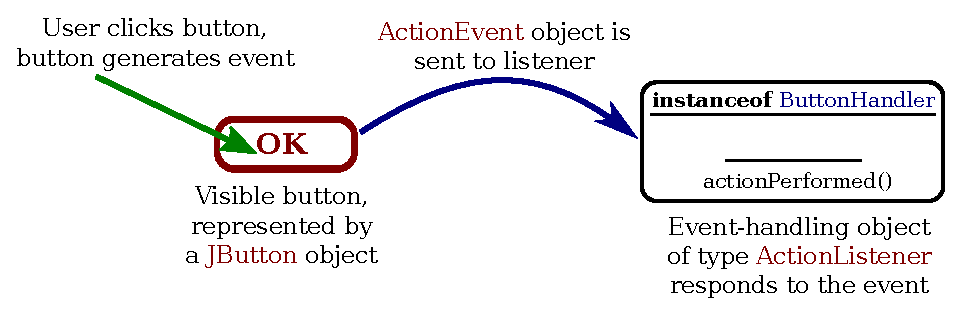
\includegraphics[scale=0.75]{images/event-handling.eps}
}

   

As an example, consider the OK button in the sample program.  When the user
clicks the button, an event is generated.  This event is represented by an object belonging
to the class \classname{ActionEvent}.  The event that is generated is associated
with the button; we say that the button is the \newword{source} of the event.
The listener object in this case is an object belonging to the class \classname{ButtonHandler},
which is defined as a nested class inside \classname{HelloWorldGUI2}:

\displaycode{private static class ButtonHandler implements ActionListener \{
   public void actionPerformed(ActionEvent e) \{
      System.exit(0);
   \}
\}}\donedisplaycode

   

This class implements the \classname{ActionListener} interface---a requirement for
listener objects that handle events from buttons.  (Interfaces were introduced in 
Section~\ref{OOP.7}.)  The event-handling method is named \code{actionPerformed},
as specified by the \classname{ActionListener} interface.  This method contains the
code that is executed when the user clicks the button; in this case, the code is simply a call
to \code{System.exit()}, which will terminate the program.
   

There is one more ingredient that is necessary to get the event from the button to the
listener object:  The listener object must \newword{register} itself with the button
as an event listener.  This is done with the statement:

\displaycode{okButton.addActionListener(listener);}\donedisplaycode

   
\noindent This statement tells \code{okButton} that when the user clicks the button, the
ActionEvent that is generated should be sent to \code{listener}.  Without this statement,
the button has no way of knowing that there is something that would like to listen for events
from the button.
   

This example shows a general technique for programming the behavior of a GUI:
Write classes that include event-handling methods.  Create objects that belong to these
classes and register them as listeners with the objects that will actually detect or
generate the events.  When an event occurs, the listener is notified, and the code that you
wrote in one of its event-handling methods is executed.  At first, this might seem like
a very roundabout and complicated way to get things done, but as you gain experience
with it, you will find that it is very flexible and that it goes together very well with
object oriented programming.


This section has introduced some of the fundamentals of GUI programming.  We will
spend the rest of the chapter exploring them in more detail.




\subsection{Some Java GUI History}\label{GUI1.1.4}



The original GUI toolkit for Java was the AWT, the ``Abstract Windowing Toolkit." It provided
a common interface to the GUI components already built into various operating systems.  At the
very beginning, it used a simpler event model that did not require listener objects, but that model
was abandoned in favor of listeners very quickly in Java~1.1.


When Java was first introduced, one of the important applications was
\newword{applets}.  An applet is a GUI program that can run on a web page
in a web browser.  Applets were covered in previous versions of this textbook,
but they have become much less widely used and have been dropped from this
seventh edition of the book.


The \newcode{Swing} GUI toolkit was introduced in Java 1.2
as an improved alternative to the AWT, with a larger variety of
sophisticated components and a more logical structure.  Although Swing uses some aspects of
the AWT, most of its components are written in Java rather than being based on operating system
components.  Swing has been the standard toolkit for writing GUI programs in Java for over
ten years, and it is the toolkit that I cover in this book.


More recently, however, another GUI toolkit called \newword{JavaFX} has been
introduced.  It uses many of the same core ideas as Swing, including components, layout, and
events, but uses a different structure for its applications and a different set of classes.
With Java~8, JavaFX becomes the preferred approach to writing GUI applications.
However, I do not cover JavaFX in this book.  JavaFX is compatible with Swing and can use
Swing components, and Swing will continue to be supported in Java.  (Indeed, the AWT is
still supported!)  And as I've said, JavaFX is built on the same core ideas as Swing.


   

   



\section{Graphics and Painting}\label{GUI1.3}



\start{{\Large E}verything you see on a computer screen} has to be
drawn there, even the text. The Java API includes a range of classes and
methods that are devoted to drawing. In this section, I'll look at some of the
most basic of these.  Some of this material was already covered in preliminary
form in Section~\ref{control.8}.


The physical structure of a GUI is built of components. The term \newword{component}
refers to a visual element in a GUI, including buttons, menus, text-input boxes, scroll bars,
check boxes, and so on. In Java,
GUI components are represented by objects belonging to subclasses of the class
\code{java.awt.Component}. Most components in the Swing GUI toolkit---although not
top-level components like JFrame---belong to subclasses of the class
\code{javax.swing.JComponent}, which is itself a subclass of \code{java.awt.Component}.
Every component is responsible for drawing
itself. If you want to use a standard component, you only have to
add it to your program. You don't have to worry about painting it on the screen.
That will happen automatically, since it already knows how to draw itself.


Sometimes, however, you do want to draw on a component. You will have to do
this whenever you want to display something that is not included among the
standard, pre-defined component classes. When you want to do this, you have to
define your own component class and provide a method in that class for drawing
the component.  I will always use a subclass of \classname{JPanel}
when I need a drawing surface of this kind, as I did for the
\classname{HelloWorldDisplay} class in the example
\sourceref{HelloWorldGUI2.java} in the 
previous section.
A JPanel, like any JComponent, draws its content in the method

\displaycode{public void paintComponent(Graphics g)}\donedisplaycode


\noindent To create a drawing surface, you should define a subclass of \code{JPanel}
and provide a custom \code{paintComponent()} method. Create an object
belonging to this class and use it in your program. When the time comes
for your component to be drawn on the screen, the system will call its
\code{paintComponent()} to do the drawing. That is, the code that you put
into the \code{paintComponent()} method will be executed whenever the
panel needs to be drawn on the screen; by writing this method, you determine
the picture that will be displayed in the panel.  Note that you are not likely to
call a \code{paintComponent()} method any more than you are likely to call
a \code{main()} routine.  The \textit{system} calls the method.  You \textit{write}
the method to say what will happen when the system calls it.


Note that the \code{paintComponent()} method has a parameter of type
\classname{Graphics}. The \classname{Graphics} object will be provided by the system
when it calls your method. You need this object to do the actual drawing. To do
any drawing at all in Java, you need a \newword{graphics context}.
A graphics context is an object belonging to the class
\code{java.awt.Graphics}.  Instance methods are provided in this class for
drawing shapes, text, and images. Any given \classname{Graphics} object can draw
to only one location. In this chapter, that location will always be a GUI
component belonging to some subclass of \code{JPanel}. The
\classname{Graphics} class is an abstract class, which means that it is impossible
to create a graphics context directly, with a constructor. There are actually
two ways to get a graphics context for drawing on a component: First of all, of
course, when the \code{paintComponent()} method of a component is called by
the system, the parameter to that method is a graphics context for drawing on
the component. Second, every component has an instance method called
\code{getGraphics()}. This method is a function that returns a graphics
context that can be used for drawing on the component outside its
\code{paintComponent()} method. The official line is that you should
\textbf{not} do this, and I will almost always avoid it. But I have
found it convenient to use \code{getGraphics()} in a few examples.
(Note that if \code{g} is a graphics context created with \code{getGraphics()},
it is good form to call \code{g.dispose()} when finished using it.  This
releases any operating system resources that might be held by~\code{g}.)
   

The \code{paintComponent()} method in the \classname{JPanel}
class simply fills the panel with the panel's background color.  When defining a
subclass of \classname{JPanel} for use as a drawing surface, you will
usually want to fill the panel with the background color before drawing
other content onto the panel (although it is not necessary to do this if the drawing
commands in the method cover the background of the component completely).
This is traditionally done with a call to
\code{super.paintComponent(g)}, so most \code{paintComponent()}
methods that you write will have the form:
   
\displaycode{public void paintComponent(g) \{
   super.paintComponent(g);
   . . . // Draw the content of the component.
\}}\donedisplaycode

   



\mybreak



In general, a component should do all drawing operations in its
\code{paintComponent()} method. What happens if, in the middle of some other
method, you realize that the content of the component needs to be changed? You
should \textbf{not} call \code{paintComponent()} directly to make the
change. Instead, you have
to inform the system that the component needs to be redrawn, and let the system
do its job by calling \code{paintComponent()}. You do this by calling the
component's \code{repaint()} method. The method

\displaycode{public void repaint();}\donedisplaycode


\noindent is defined in the \code{Component} class, and so can be used with any
component. You should call \code{repaint()} to inform the system that the
component needs to be redrawn. It is important to understand that the 
\code{repaint()} method returns
immediately, without doing any painting itself. The system will call the
component's \code{paintComponent()} method \textit{later}, as soon as it gets
a chance to do so, after processing other pending events if there are any.
It is even possible that many calls to \code{repaint()} will all be handled
by one call to \code{paintComponent()}, if the calls to \code{repaint()}
occur in a very short timespan.


Note that the system can also call \code{paintComponent()} for other
reasons. It is called when the component first appears on the screen. It will
also be called if the size of the component changes, which can happen when
the user resizes the window that contains the component.  This means that
\code{paintComponent()} should be capable of redrawing the content
of the component on demand.  As you will see, however, some of our early examples 
will not be able to do this correctly.


This means that, to work properly, the \code{paintComponent()} method must
be smart enough to correctly redraw the component at any time. To make this
possible, a program should store data in its instance variables
about the state of the component. These variables should contain all the information
necessary to redraw the component completely. The \code{paintComponent()}
method should use the data in these variables to decide what to draw. When the
program wants to change the content of the component, it should not simply draw
the new content. It should change the values of the relevant variables and call
\code{repaint()}. When the system calls \code{paintComponent()}, that
method will use the new values of the variables and will draw the component
with the desired modifications. This might seem a roundabout way of doing
things. Why not just draw the modifications directly? There are at least two
reasons. First of all, it really does turn out to be easier to get things right
if all drawing is done in one method. Second, even if you could directly
draw the modifications, you would still have to save enough information about
the modifications to enable \code{paintComponent()}
to \textbf{redraw} the component correctly on demand.


You will see how all this works in practice as we work through examples in
the rest of this chapter. For now, we will spend the rest of this section
looking at how to get some actual drawing done.

\subsection{Coordinates}\label{GUI1.3.1}



The screen of a computer is a grid of little squares called \newword{pixels}.
The color of each pixel can be set individually, and
drawing on the screen just means setting the colors of individual pixels.


\par\dumpfigure{
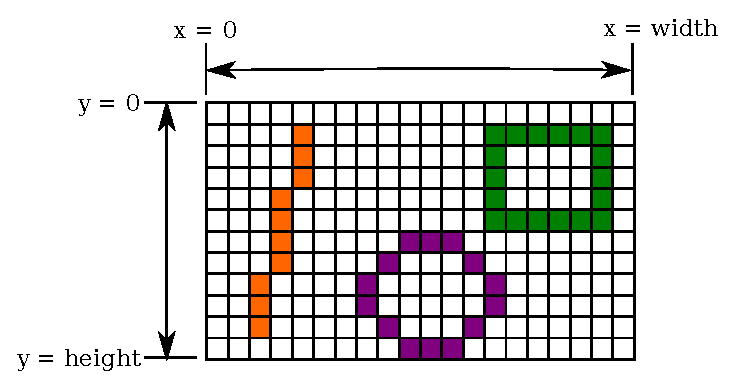
\includegraphics[scale=0.75]{images/pixel-coordinates.eps}
}



A graphics context draws in a rectangle made up of pixels. A position in the
rectangle is specified by a pair of integer coordinates, \code{(x,y)}. The
upper left corner has coordinates \code{(0,0)}. The \code{x} coordinate
increases from left to right, and the \code{y} coordinate increases from top
to bottom. The illustration shows a 20-pixel by 12-pixel component (with
very large pixels). A small line, rectangle, and oval are shown as they would
be drawn by coloring individual pixels. (Note that, properly speaking, the
coordinates don't belong to the pixels but to the grid lines between them.)


For any component, you can find out the size of the rectangle that it
occupies by calling the instance methods \code{getWidth()} and
\code{getHeight()}, which return the number of pixels in the
horizontal and vertical directions, respectively.  In general, it's not
a good idea to assume that you know the size of a component, since the
size is often set by a layout manager and can even change if the component
is in a window and that window is resized by the user.   This means that it's good
form to check the size of a component before doing any drawing on that
component. For example, you can use a \code{paintComponent()} method that
looks like:

\displaycode{public void paintComponent(Graphics g) \{
   super.paintComponent(g);
   int width =  getWidth();   // Find out the width of this component.
   int height = getHeight();  // Find out its height.
   . . .   // Draw the content of the component.
\}}\donedisplaycode



Of course, your drawing commands will have to take the size into account.
That is, they will have to use \code{(x,y)} coordinates that are calculated
based on the actual height and width of the component.  (However, if you are
sure that you know the size, using constants for the width and height can
make the drawing easier.)


   
\subsection{Colors}\label{GUI1.3.2}

   

You will probably want to use some color when you draw.
Java is designed to work with the \newword{RGB color system}.
An RGB color is specified by three numbers that give the level
of red, green, and blue, respectively, in the color. A color in Java is an
object of the class, \code{java.awt.Color}. You can construct a new color by
specifying its red, blue, and green components. For example,

\displaycode{Color myColor = new Color(r,g,b);}\donedisplaycode


\noindent There are two constructors that you can call in this way. In the one that I
almost always use, \code{r}, \code{g}, and \code{b} are integers in the
range 0 to 255. In the other, they are numbers of type \ptype{float} in the
range 0.0F to 1.0F. (Recall that a literal of type \ptype{float} is
written with an ``F" to distinguish it from a \ptype{double} number.) Often,
you can avoid constructing new colors altogether, since the \classname{Color}
class defines several named constants representing common colors: \code{Color.WHITE},
\code{Color.BLACK}, \code{Color.RED}, \code{Color.GREEN},
\code{Color.BLUE}, \code{Color.CYAN}, \code{Color.MAGENTA},
\code{Color.YELLOW}, \code{Color.PINK}, \code{Color.ORANGE},
\code{Color.LIGHT\_GRAY}, \code{Color.GRAY}, and \code{Color.DARK\_GRAY}.
(There are older, alternative names for these constants that use lower case rather than
upper case constants, such as \code{Color.red} instead of \code{Color.RED},
but the upper case versions are preferred because they follow the convention that
constant names should be upper case.)


An alternative to RGB is the \newword{HSB color system}.
In the HSB system, a color is specified by three numbers called the
\newword{hue}, the \newword{saturation},
and the \newword{brightness}. The hue is the basic color,
ranging from red through orange through all the other colors of the rainbow.
The brightness is pretty much what it sounds like. A fully saturated color is a
pure color tone. Decreasing the saturation is like mixing white or gray paint
into the pure color. In Java, the hue, saturation and brightness are always
specified by values of type \ptype{float} in the range from 0.0F to 1.0F. The
\classname{Color} class has a \code{static} member function named
\code{getHSBColor} for creating HSB colors. To create the color with HSB
values given by \code{h}, \code{s}, and \code{b}, you can say:

\displaycode{Color myColor = Color.getHSBColor(h,s,b);}\donedisplaycode


\noindent For example, to make a color with a random hue that is as bright and as
saturated as possible, you could use:

\displaycode{Color randomColor = Color.getHSBColor( (float)Math.random(), 1.0F, 1.0F );}\donedisplaycode


\noindent The type cast is necessary because the value returned by
\code{Math.random()} is of type \ptype{double}, and
\code{Color.getHSBColor()} requires values of type \ptype{float}. (By the
way, you might ask why RGB colors are created using a constructor while HSB
colors are created using a static member function. The problem is that we would
need two different constructors, both of them with three parameters of type
\ptype{float}. Unfortunately, this is impossible. You can have two
constructors only if the number of parameters or the parameter types differ.)


The RGB system and the HSB system are just different ways of describing the
same set of colors. It is possible to translate between one system and the
other. The best way to understand the color systems is to experiment with them.
(The sample program \sourceref{SimpleColorChooser.java} lets you do that.
You won't understand the source code at this time, but you can run it to play
with color selection or to find the RGB or HSB values for the color that want.)


\mybreak



One of the properties of a \classname{Graphics} object is the current
drawing color, which is used for all drawing of shapes and text. If \code{g}
is a graphics context, you can change the current drawing color for \code{g}
using the method \code{g.setColor(c)}, where \code{c} is a \classname{Color}.
For example, if you want to draw in green, you would just say
\code{g.setColor(Color.GREEN)} before doing the drawing. The graphics context
continues to use the color until you explicitly change it with another
\code{setColor()} command. If you want to know what the current drawing color
is, you can call the function \code{g.getColor()}, which returns an object of
type \classname{Color}. This can be useful if you want to change to another
drawing color temporarily and then restore the previous drawing color.


Every component has an associated \newword{foreground color} and 
\newword{background color}. Generally, the
component is filled with the background color before anything else is drawn
(although some components are ``transparent," meaning that the background color
is ignored). When a new graphics context is created for a component, the
current drawing color is set to the foreground color. Note that the foreground
color and background color are properties of the component, not of a graphics
context.


The foreground and background colors of a component can be set by calling instance methods
\code{component.setForeground(color)} and \code{component.setBackground(color)}, which are defined in
the \classname{Component} class and therefore are available for use with any
component.  This can be useful even for standard components, if you want them
to use colors that are different from the defaults.


   
\subsection{Fonts}\label{GUI1.3.3}

   

A \newword{font} represents a particular size and style
of text. The same character will appear different in different fonts. In Java,
a font is characterized by a font name, a style, and a size. The available font
names are system dependent, but you can always use the following four strings
as font names: ``Serif", ``SansSerif", ``Monospaced", and ``Dialog".  (A ``serif" is a
little decoration on a character, such as a short horizontal line at the bottom
of the letter~i. ``SansSerif" means ``without serifs." ``Monospaced" means that
all the characters in the font have the same width. The ``Dialog" font is the
one that is typically used in dialog boxes.)


The style of a font is specified using named constants that are defined in
the \classname{Font} class. You can specify the style as one of the four
values:



\mylist{

\myitem \code{Font.PLAIN},
\myitem \code{Font.ITALIC},
\myitem \code{Font.BOLD}, or
\myitem \code{Font.BOLD + Font.ITALIC}.
}



The size of a font is an integer. Size typically ranges from about 9 to 36,
although larger sizes can also be used. The size of a font is usually about
equal to the height of the largest characters in the font, in pixels, but this
is not an exact rule. The size of the default font is 12.


Java uses the class named \code{java.awt.Font} for representing fonts. You
can construct a new font by specifying its font name, style, and size in a
constructor:

\displaycode{Font plainFont = new Font("Serif", Font.PLAIN, 12);
Font bigBoldFont = new Font("SansSerif", Font.BOLD, 24);}\donedisplaycode



Every graphics context has a current font, which is used for drawing text.
You can change the current font with the \code{setFont()} method. For
example, if \code{g} is a graphics context and \code{bigBoldFont} is a
font, then the command \code{g.setFont(bigBoldFont)} will set the current
font of \code{g} to \code{bigBoldFont}. The new font will be used
for any text that is drawn \textit{after} the \code{setFont()} command is given.
You can find out the current font
of \code{g} by calling the method \code{g.getFont()}, which returns an
object of type \classname{Font}.


Every component also has an associated font. It can be set with the instance
method \code{component.setFont(font)}, which is defined in the \classname{Component}
class. When a graphics context is created for drawing on a component, the
graphic context's current font is set equal to the font of the component.


   
\subsection{Shapes}\label{GUI1.3.4}



The \classname{Graphics} class includes a large number of instance methods for
drawing various shapes, such as lines, rectangles, and ovals. The shapes are
specified using the \code{(x,y)} coordinate system described above. They are
drawn in the current drawing color of the graphics context. The current drawing
color is set to the foreground color of the component when the graphics context
is created, but it can be changed at any time using the \code{setColor()}
method.


Some drawing methods were already listed in Subsection~\ref{control.8.1}.
Here, I describe those methods in more detail and add a few more.
With all these
commands, any drawing that is done outside the boundaries of the component is
ignored. Note that all these methods are in the \classname{Graphics} class, so
they all must be called through an object of type \classname{Graphics}.
It is shown here as \code{g}, but of course
the name of the graphics context is up to the programmer.



\mylist{

\myitem \codedef{g.drawString(String str, int x, int y)} --- Draws
the text given by the string \code{str}. The string is drawn using
the current color and font of the graphics context. \code{x} specifies the
x-coordinate of the left end of the string. \code{y} is the y-coordinate of the
baseline of the string. The baseline is a horizontal line on which the
characters rest. Some parts of the characters, such as the tail on a y or g,
extend below the baseline.
\myitem \codedef{g.drawLine(int x1, int y1, int x2, int y2)} --- Draws 
a line from the point \code{(x1,y1)} to the point
\code{(x2,y2)}. The line is drawn as if with a pen that extends one pixel to
the right and one pixel down from the \code{(x,y)} point where the pen is
located. For example, if \code{g} refers to an object of type
\classname{Graphics}, then the command \code{g.drawLine(x,y,x,y)}, which
corresponds to putting the pen down at a point, colors the single pixel with upper left corner
at the point \code{(x,y)}.  Remember that coordinates really refer to the lines
between the pixels.
\myitem \codedef{g.drawRect(int x, int y, int width, int height)} --- Draws 
the outline of a rectangle. The upper left corner
is at \code{(x,y)}, and the width and height of the rectangle are as
specified. If \code{width} equals \code{height}, then the rectangle is a
square. If the \code{width} or the \code{height} is negative, then nothing
is drawn. The rectangle is drawn with the same pen that is used for
\code{drawLine()}. This means that the actual width of the rectangle as drawn
is \code{width+1}, and similarly for the height. There is an extra pixel
along the right edge and the bottom edge. For example, if you want to draw a
rectangle around the edges of the component, you can say ``\code{g.drawRect(0, 0,
getWidth()-1, getHeight()-1);}".  If you use ``\code{g.drawRect(0, 0,
getWidth(), getHeight());}", then the right and bottom edges of the
rectangle will be drawn \textit{outside} the component and will not appear
on the screen.
\myitem \codedef{g.drawOval(int x, int y, int width, int height)} --- Draws
the outline of an oval. The oval is one that just
fits inside the rectangle specified by \code{x}, \code{y}, \code{width},
and \code{height}. If \code{width} equals \code{height}, the oval is a
circle.
\myitem \codedef{g.drawRoundRect(int x, int y, int width, int height,
int xdiam, int ydiam)} --- Draws the outline of a rectangle with
rounded corners. The basic rectangle is specified by \code{x}, \code{y},
\code{width}, and \code{height}, but the corners are rounded. The degree of
rounding is given by \code{xdiam} and \code{ydiam}. The corners are arcs of
an ellipse with horizontal diameter \code{xdiam} and vertical diameter
\code{ydiam}. A typical value for \code{xdiam} and \code{ydiam} is 16,
but the value used should really depend on how big the rectangle is.
\myitem \codedef{g.draw3DRect(int x, int y, int width, int height,
boolean raised)} --- Draws the outline of a rectangle that is
supposed to have a three-dimensional effect, as if it is raised from the screen
or pushed into the screen. The basic rectangle is specified by \code{x},
\code{y}, \code{width}, and \code{height}. The \code{raised} parameter
tells whether the rectangle seems to be raised from the screen or pushed into
it. The 3D effect is achieved by using brighter and darker versions of the
drawing color for different edges of the rectangle. The documentation
recommends setting the drawing color equal to the background color before using
this method. The effect won't work well for some colors.
\myitem \codedef{g.drawArc(int x, int y, int width, int height, int
startAngle, int arcAngle)} --- Draws part of the oval that just fits
inside the rectangle specified by \code{x}, \code{y}, \code{width}, and
\code{height}. The part drawn is an arc that extends \code{arcAngle}
degrees from a starting angle at \code{startAngle} degrees. Angles are
measured with 0 degrees at the 3 o'clock position (the positive direction of
the horizontal axis). Positive angles are measured counterclockwise from zero,
and negative angles are measured clockwise. To get an arc of a circle, make
sure that \code{width} is equal to \code{height}.
\myitem \codedef{g.fillRect(int x, int y, int width, int
height)} --- Draws a filled-in rectangle. This fills in the interior
of the rectangle that would be drawn by \code{drawRect(x,y,width,height)}.
The extra pixel along the bottom and right edges is not included. The
\code{width} and \code{height} parameters give the exact width and height
of the rectangle. For example, if you wanted to fill in the entire component,
you could say ``\code{g.fillRect(0, 0, getWidth(),
getHeight());}"
\myitem \codedef{g.fillOval(int x, int y, int width, int
height)} --- Draws a filled-in oval.
\myitem \codedef{g.fillRoundRect(int x, int y, int width, int height,
int xdiam, int ydiam)} --- Draws a filled-in rounded rectangle.
\myitem \codedef{g.fill3DRect(int x, int y, int width, int height,
boolean raised)} --- Draws a filled-in three-dimensional
rectangle.
\myitem \codedef{g.fillArc(int x, int y, int width, int height, int
startAngle, int arcAngle)} --- Draw a filled-in arc. This looks like
a wedge of pie, whose crust is the arc that would be drawn by the
\code{drawArc} method.
}

   

   
\subsection{Graphics2D}\label{GUI1.3.5}



All drawing in Java is done through an object of type \classname{Graphics}. The
\classname{Graphics} class provides basic commands for such things as drawing
shapes and text and  for selecting a drawing color. These commands are adequate in many cases, but
they fall far short of what's needed in a serious computer graphics program.
Java has another class, \classname{Graphics2D}, that provides a larger
set of drawing operations. \classname{Graphics2D} is a sub-class of
\classname{Graphics}, so all the methods from the \classname{Graphics} class are
also available in a \classname{Graphics2D}.


The \code{paintComponent()} method of a \code{JComponent} gives you a
graphics context of type \classname{Graphics} that you can use for drawing on the
component. In fact, the graphics context actually belongs to the sub-class
\classname{Graphics2D}, and can be type-cast to
gain access to the advanced \classname{Graphics2D} drawing methods:

\displaycode{public void paintComponent(Graphics g) \{
   super.paintComponent(g);
   Graphics2D g2;
   g2 = (Graphics2D)g;
    .
    . // Draw on the component using g2.
    .
\}}\donedisplaycode



I mention \classname{Graphics2D} here for completeness.
I will cover some important aspects of \classname{Graphics2D}
in Section~\ref{GUI2.2}, but a full treatment is more than we will have
time for in this book.  However, there are two simple applications 
that I would like to start using now, without explaining how they work.
If \code{g2} is a variable of type \classname{Graphics2D}, 
as in the \code{paintComponent()} method above, then the 
intimidating-looking command

\displaycode{g2.setRenderingHint( RenderingHints.KEY\_ANTIALIASING, 
                                RenderingHints.VALUE\_ANTIALIAS\_ON );}\donedisplaycode


\noindent turns on antialiasing in the graphics context.  Aliasing is a jagged appearance
that can be seen when shapes are drawn using pixels.  Antialiasing tries to reduce
the jaggedness.  It can make diagonal lines and the outlines of ovals look much nicer.
It can also improve the appearance of text.  Another useful command is

\displaycode{g2.setStroke( new BasicStroke(lineWidth) );}\donedisplaycode


\noindent where \code{lineWidth} is an integer or a float.  This command can be use to
draw thicker lines.  Lines drawn after the command will be \code{lineWidth} pixels
wide.  This also affects the thickness of the outlined shapes drawn by methods such as
\code{g.drawRect} and \code{g.drawOval()}.



\subsection{An Example}\label{GUI1.3.6}

   

Let's use some of the material covered in this section to write a subclass
of \classname{JPanel} for use as a drawing surface.  
All the drawing will be done in the
\code{paintComponent()} method of the panel class.
The panel will draw multiple copies of a message on a black background.
Each copy of the message is in a random color. Five different fonts are used,
with different sizes and styles. The message can be specified in the constructor;
if the default constructor is used, the message is the string ``Java!". The
panel works OK no matter what  its size.


There is one problem with the way this class works. When the panel's
\code{paintComponent()} method is called, it chooses random colors, fonts,
and locations for the messages. The information about which colors, fonts, and
locations are used is not stored anywhere. The next time
\code{paintComponent()} is called, it will make different random choices and
will draw a different picture.  If you resize a window containing the panel,
the picture will be continually redrawn as the size of the window is changed!
To avoid that, you would store enough information about the picture in instance variables
to enable the \code{paintComponent()} method to draw the same picture each
time it is called.


The source code for the panel class is shown below. I use an instance variable called
\code{message} to hold the message that the panel will display. There are
five instance variables of type \classname{Font} that represent different sizes
and styles of text. These variables are initialized in the constructor
and are used in the \code{paintComponent()} method.


The \code{paintComponent()} method for the panel simply draws 25
copies of the message. For each copy, it chooses one of the five fonts at
random, and it uses \code{g.setFont()} to select that font for drawing.
It creates a random HSB color and uses \code{g.setColor()} to select
that color for drawing. It then chooses random \code{(x,y)} coordinates for
the location of the message. The \code{x} coordinate gives the horizontal
position of the left end of the string. The formula used for the \code{x}
coordinate is ``\code{-50~+ (int)(Math.random() * (width+40))}". This gives a random
integer in the range from \code{-50} to \code{width-10}. This makes it
possible for the string to extend beyond the left edge or the right edge of the
panel. Similarly, the formula for \code{y} allows the string to extend
beyond the top and bottom.



Here is the complete source code for the \classname{RandomStringsPanel}:

\displaycode{import java.awt.*;
import javax.swing.JPanel;

/**
 * This panel displays 25 copies of a message.  The color and 
 * position of each message is selected at random.  The font
 * of each message is randomly chosen from among five possible
 * fonts.  The messages are displayed on a black background.
 * Note:  The style of drawing used here is poor, because every
 * time the paintComponent() method is called, new random values are
 * used.  This means that a different picture will be drawn each time.  
 */
public class RandomStringsPanel extends JPanel \{

    private String message;  // The message to be displayed.  This can be set in
                             // the constructor.  If no value is provided in the
                             // constructor, then the string "Java!" is used.

    private Font font1, font2, font3, font4, font5;  // The five fonts.

    /**
     * Default constructor creates a panel that displays the message "Java!".
     */
    public RandomStringsPanel() \{
        this(null);  // Call the other constructor, with parameter null.
    \}

    /**
     * Constructor creates a panel to display 25 copies of a specified message.
     * @param messageString The message to be displayed.  If this is null,
     * then the default message "Java!" is displayed.
     */
    public RandomStringsPanel(String messageString) \{

        message = messageString;
        if (message == null)
            message = "Java!";

        font1 = new Font("Serif", Font.BOLD, 14);
        font2 = new Font("SansSerif", Font.BOLD + Font.ITALIC, 24);
        font3 = new Font("Monospaced", Font.PLAIN, 30);
        font4 = new Font("Dialog", Font.PLAIN, 36);
        font5 = new Font("Serif", Font.ITALIC, 48);

        setBackground(Color.BLACK);

    \}

    /**
     * The paintComponent method is responsible for drawing the content of the panel.
     * It draws 25 copies of the message string, using a random color, font, and
     * position for each string.
     */
    public void paintComponent(Graphics g) \{

        super.paintComponent(g);  // Call the paintComponent method from the 
                                  // superclass, JPanel.  This simply fills the 
                                  // entire panel with the background color, black.
        
        Graphics2D g2 = (Graphics2D)g;  // (To make the text smoother.)
        g2.setRenderingHint( RenderingHints.KEY\_ANTIALIASING, 
                                RenderingHints.VALUE\_ANTIALIAS\_ON );

        int width = getWidth();
        int height = getHeight();

        for (int i = 0; i \< 25; i++) \{

            // Draw one string.  First, set the font to be one of the five
            // available fonts, at random.  

            int fontNum = (int)(5*Math.random()) + 1;
            switch (fontNum) \{
            case 1:
                g.setFont(font1);
                break;
            case 2:
                g.setFont(font2);
                break;
            case 3:
                g.setFont(font3);
                break;
            case 4:
                g.setFont(font4);
                break;
            case 5:
                g.setFont(font5);
                break;
            \} // end switch

            // Set the color to a bright, saturated color, with random hue.

            float hue = (float)Math.random();
            g.setColor( Color.getHSBColor(hue, 1.0F, 1.0F) );

            // Select the position of the string, at random.

            int x,y;
            x = -50 + (int)(Math.random()*(width+40));
            y = (int)(Math.random()*(height+20));

            // Draw the message.

            g.drawString(message,x,y);

        \} // end for

    \} // end paintComponent()


\}  // end class RandomStringsPanel
}\donedisplaycode

  
   



\subsection{Where is main()?}\label{GUI1.3.7}



The source code for the \classname{RandomStringsPanel} class can be 
found in the example file \sourceref{RandomStringsPanel.java}.  You can
compile that file, but you won't be able to run the compiled class.  The problem is
that the class doesn't have a \code{main()} routine.  Only a class that has a
\code{main()} routine can be run as a program.


Another problem is that a \classname{JPanel} is not something that
can stand on its own.  It has to be placed into a container such as another
panel or a window.  In general, to make a complete program, we need a \code{main()}
routine that will create a window of type \classname{JFrame}.  It can then
create a panel and place the panel in the window.  Here is a class with a
\code{main()} routine that does this:

\displaycode{
import javax.swing.JFrame;

public class RandomStrings \{
    
    public static void main(String[] args) \{
        JFrame window = new JFrame("Java!");
        RandomStringsPanel content = new RandomStringsPanel();
        window.setContentPane(content);
        window.setDefaultCloseOperation(JFrame.EXIT\_ON\_CLOSE);
        window.setLocation(120,70);
        window.setSize(350,250);
        window.setVisible(true);
    \}

\}}\donedisplaycode


\noindent This class is defined by the file \sourceref{RandomStrings.java}.  You can compile
and run the program, as long as the \classname{RandomStringsPanel} class is also 
available.


The main routine is not logically a part of the panel class.  It is just one way
of using a panel.  However, it's possible to include \code{main()} as part of the
panel class, even if it doesn't logically belong there.  This makes it possible to run
the panel class as a program, and it has the advantage of keeping everything in one
file.  For an example, you can look at
\sourceref{RandomStringsPanelWithMain.java}, which is identical to
the original class except for the addition of a \code{main()} routine.
Although it might not be great style, I will usually take a similar approach
in future examples.


I am not going to discuss the
details of using \classname{JFrame} here, but you can look ahead
and find them in Subsection~\ref{GUI1.8.3}.  You won't completely understand
my \code{main()} routines until you read that section.

   

   

   



\section{Mouse Events}\label{GUI1.4}

   

\start{{\Large E}vents are central} to programming for a graphical
user interface. A GUI program doesn't have a \code{main()} routine that
outlines what will happen when the program is run, in a step-by-step process
from beginning to end. Instead, the program must be prepared to respond to
various kinds of events that can happen at unpredictable times and in an order
that the program doesn't control. The most basic kinds of events are generated
by the mouse and keyboard. The user can press any key on the keyboard, move the
mouse, or press a button on the mouse. The user can do any of these things at
any time, and the computer has to respond appropriately.


In Java, events are represented by objects. When an event occurs, the system
collects all the information relevant to the event and constructs an object to
contain that information. Different types of events are represented by objects
belonging to different classes. For example, when the user presses one of the
buttons on a mouse, an object belonging to a class called \classname{MouseEvent}
is constructed. The object contains information such as the source of the event (that is, the component on
which the user clicked), the \code{(x,y)} coordinates of the point in the
component where the click occurred, the exact time of the click, and which button on the mouse was pressed.
When the user presses a key on the keyboard, a \classname{KeyEvent} is created.
After the event object is constructed, it can be passed as a parameter to a
designated method. By writing that method, the programmer says what
should happen when the event occurs.


As a Java programmer, you get a fairly high-level view of events. There is a
lot of processing that goes on between the time that the user presses a key or
moves the mouse and the time that a subroutine in your program is called to
respond to the event. Fortunately, you don't need to know much about that
processing. But you should understand this much: Even though you didn't
write it, there is a routine running somewhere that executes a loop of the form

\displaycode{while the program is still running:
    Wait for the next event to occur
    Call a subroutine to handle the event}\donedisplaycode



This loop is called an \newword{event loop}. Every GUI
program has an event loop. In Java, you don't have to write the loop. It's part
of ``the system." If you write a GUI program in some other language, you might
have to provide a main routine that runs the event loop.


In this section, we'll look at handling mouse events in Java, and we'll
cover the framework for handling events in general. The next
section will cover keyboard-related events and timer events. 
Java also has other types of events, which are produced by GUI components.
These will be introduced in Section~\ref{GUI1.6}.

\subsection{Event Handling}\label{GUI1.4.1}



For an event to have any effect, a program must detect the event and react
to it. In order to detect an event, the program must ``listen" for it. Listening
for events is something that is done by an object called an \newword{event listener}. 
An event listener object must contain instance
methods for handling the events for which it listens. For example, if an object
is to serve as a listener for events of type \classname{MouseEvent}, then it must
contain the following method (among several others):

\displaycode{public void mousePressed(MouseEvent evt) \{ . . . \}}\donedisplaycode


\noindent The body of the method defines how the object responds when it is notified
that a mouse button has been pressed. The parameter, \code{evt}, contains
information about the event. This information can be used by the listener
object to determine its response.


The methods that are required in a mouse event listener are specified in an
\code{interface} named \classname{MouseListener}. To be used as a listener for
mouse events, an object must implement this \classname{MouseListener} interface.
Java \code{interfaces} were covered in Section~\ref{OOP.7}. 
(To review briefly: An \code{interface} in Java is just a list of
instance methods. A class can ``implement" an interface by doing two things:
First, the class must be declared to implement the interface, as in ``\code{class
MouseHandler implements MouseListener}" or ``\code{class MyPanel extends
JPanel implements MouseListener}";  and second, the class must include a
definition for each instance method specified in the interface. An
\code{interface} can be used as the type for a variable or formal parameter.
We say that an \textit{object} implements the \classname{MouseListener} interface if it
belongs to a \textit{class} that implements the \classname{MouseListener} interface. Note
that it is not enough for the object to include the specified methods. It must
also belong to a class that is specifically declared to implement the
interface.)


Many events in Java are associated with GUI components. For example, when
the user presses a button on the mouse, the associated component is the one
that the user clicked on. Before a listener object can ``hear" events associated
with a given component, the listener object must be registered with the
component. If a \classname{MouseListener} object, \code{mListener}, needs to
hear mouse events associated with a \classname{Component} object, \code{comp}, the
listener must be \newword{registered} with the component by
calling

\displaycode{comp.addMouseListener(mListener);}\donedisplaycode
 

\noindent The \code{addMouseListener()} method is an instance method in class
\classname{Component}, and so can be used with any GUI component object. In our
first few examples, we will listen for events on a \classname{JPanel} that is being used as
a drawing surface.


The event classes, such as \classname{MouseEvent}, and the listener interfaces,
such as \classname{MouseListener}, are defined in the package
\code{java.awt.event}. This means that if you want to work with events, you
should either include the line ``\code{import java.awt.event.*;}" at the beginning of
your source code file or import the individual classes and interfaces.


Admittedly, there is a large number of details to tend to when you want to
use events. To summarize, you must



\mynumberedlist{

\mynumbereditem Put the import specification ``\code{import java.awt.event.*;}" (or individual imports)
at the beginning of your source code;
\mynumbereditem Declare that some class implements the appropriate listener interface, such
as \classname{MouseListener};
\mynumbereditem Provide definitions in that class for the methods specified by the
interface;
\mynumbereditem Register an object that belongs to the listener class 
with the component that will generate the
events by calling a method such as \code{addMouseListener()} in the
component.
}



Any object can act as an event listener, provided that it implements the
appropriate interface. A component can listen for the events that it itself
generates. A panel can listen for events from components that are contained
in the panel. A special class can be created just for the purpose of defining
a listening object. Many people consider it to be good form to use anonymous
inner classes to define listening objects (see Subsection~\ref{OOP.8.3}),
and named nested classes can also be appropriate.
You will see all of these patterns in examples in this textbook.


   
\subsection{MouseEvent and MouseListener}\label{GUI1.4.2}



The \classname{MouseListener} interface specifies these five instance
methods:

\displaycode{public void mousePressed(MouseEvent evt);
public void mouseReleased(MouseEvent evt);
public void mouseClicked(MouseEvent evt);
public void mouseEntered(MouseEvent evt);
public void mouseExited(MouseEvent evt);}\donedisplaycode



The \code{mousePressed} method is called as soon as the user presses down
on one of the mouse buttons, and \code{mouseReleased} is called when the user
releases a button. These are the two methods that are most commonly used, but
any mouse listener object must define all five methods; you can leave the body
of a method empty if you don't want to define a response. The
\code{mouseClicked} method is called if the user presses a mouse button and
then releases it, without moving the mouse. (When the user does this,
all three routines---\code{mousePressed}, \code{mouseReleased}, and
\code{mouseClicked}---will be called in that order.) In most cases, you
should define \code{mousePressed} instead of \code{mouseClicked}. The
\code{mouseEntered} and \code{mouseExited} methods are called when the
mouse cursor enters or leaves the component. For example, if you want the
component to change appearance whenever the user moves the mouse over the
component, you could define these two methods.


As a first example, we will look at a small addition to the \classname{RandomStringsPanel}
example from the previous section. In the new version,
the panel will repaint itself when the user clicks on it.  In order for this to happen,
a mouse listener should listen for mouse events on the panel, and when the listener
detects a \code{mousePressed} event, it should respond by calling the
\code{repaint()} method of the panel.

   

For the new version of the program, we need an object that implements the
\classname{MouseListener} interface.  One way to create the
object is to define a separate class, such as:

\displaycode{import java.awt.Component;
import java.awt.event.*;

/**
 * An object of type RepaintOnClick is a MouseListener that
 * will respond to a mousePressed event by calling the repaint()
 * method of the source of the event.  That is, a RepaintOnClick
 * object can be added as a mouse listener to any Component;
 * when the user clicks that component, the component will be
 * repainted.
 */
public class RepaintOnClick implements MouseListener \{

   public void mousePressed(MouseEvent evt) \{
      Component source = (Component)evt.getSource();
      source.repaint();  // Call repaint() on the Component that was clicked.
   \}

   public void mouseClicked(MouseEvent evt) \{ \}
   public void mouseReleased(MouseEvent evt) \{ \}
   public void mouseEntered(MouseEvent evt) \{ \}
   public void mouseExited(MouseEvent evt) \{ \}

\}}\donedisplaycode


\noindent This class does three of the four things that we need to do in order
to handle mouse events:  First, it imports \code{java.awt.event.*}
for easy access to event-related classes.  Second, it is declared that
the class ``\code{implements MouseListener}".  And third, it provides
definitions for the five methods that are specified in the
\classname{MouseListener} interface.  (Note that four of the 
methods have empty bodies, since we don't want to do anything in response
to those events.)
   

We must do one more thing to set up the event handling for this example:
We must register an event-handling object as a listener with the component
that will generate the events.  In this case, the mouse events that we are
interested in will be generated by an object of type \classname{RandomStringsPanel}.
If \code{panel} is a variable that refers to the panel object,
we can create a mouse listener object and register it with the panel with
the statements:
  
\displaycode{RepaintOnClick listener = new RepaintOnClick();  // Create MouseListener object.
panel.addMouseListener(listener);  // Register MouseListener with the panel.}\donedisplaycode

 
\noindent This could be done, for example, in the \code{main()} routine where
the panel is created.  Once the \code{listener} has been registered in this way,
it will be notified of
mouse events on the panel.  When a \code{mousePressed} event occurs, the
\code{mousePressed()} method in the \code{listener} will be called.
The code in this method calls the \code{repaint()} method in the
component that is the source of the event, that is, in the panel.  The result
is that the \code{RandomStringsPanel} is repainted with its strings
in new random colors, fonts, and positions.
   

Although we have written the \classname{RepaintOnClick} class for use
with our \classname{RandomStringsPanel} example, the event-handling
class contains no reference at all to the \classname{RandomStringsPanel}
class.  How can this be?  The \code{mousePressed()} method in
class \classname{RepaintOnClick} looks at the source of the event,
and calls its \code{repaint()} method.  If we have registered the
\classname{RepaintOnClick} object as a listener on a
\classname{RandomStringsPanel}, then it is that panel that is
repainted.  But the listener object could be used with any type of component,
and it would work in the same way.
   

Similarly, the \classname{RandomStringsPanel} class contains no
reference to the \classname{RepaintOnClick} class---in fact,
\classname{RandomStringsPanel} was written before we even knew
anything about mouse events!  The panel will
send mouse events to any object that has registered with it as a mouse listener.
It does not need to know anything about that object except that it is capable
of receiving mouse events.
   

The relationship between an object that generates an event and an object
that responds to that event is rather loose.   The relationship is set up by
registering one object to listen for events from the other object.  This is
something that can potentially be done from outside both objects.  Each object
can be developed independently, with no knowledge of the internal operation
of the other object.  This is the essence of \newword{modular design}:  Build a complex
system out of modules that interact only in straightforward, easy to understand
ways.  Then each module is a separate design problem that can be tackled independently.
Java's event-handling framework is designed to offer strong support for
modular design.
   
   

To make this clearer, let's look at a new version of \sourceref{RandomStrings.java},
the program from Subsection~\ref{GUI1.3.7} that uses \classname{RandomStringsPanel}.
The new version is \sourceref{ClickableRandomStrings.java}.  For convenience, I have added
\classname{RepaintOnClick} as a static nested class, although it would work just as well
as a separate class:
   
\displaycode{import java.awt.Component;
import java.awt.event.MouseEvent;
import java.awt.event.MouseListener;
import javax.swing.JFrame;

/**
 * Displays a window that shows 25 copies of the string "Java!" in
 * random colors, fonts, and positions.  The content of the window
 * is an object of type RandomStringsPanel.  When the user clicks
 * the window, the content of the window is repainted, with the 
 * strings in newly selected random colors, fonts, and positions.
 */
public class ClickableRandomStrings \{
    
    public static void main(String[] args) \{
        JFrame window = new JFrame("Click Me to Redraw!");
        RandomStringsPanel content = new RandomStringsPanel();
        \newcode{content.addMouseListener( new RepaintOnClick() );}        
        window.setContentPane(content);
        window.setDefaultCloseOperation(JFrame.EXIT\_ON\_CLOSE);
        window.setLocation(120,70);
        window.setSize(350,250);
        window.setVisible(true);
    \}
    
    private static class RepaintOnClick implements MouseListener \{

        public void mousePressed(MouseEvent evt) \{
            Component source = (Component)evt.getSource();
            source.repaint();
        \}

        public void mouseClicked(MouseEvent evt) \{ \}
        public void mouseReleased(MouseEvent evt) \{ \}
        public void mouseEntered(MouseEvent evt) \{ \}
        public void mouseExited(MouseEvent evt) \{ \}

    \}

\} end class ClickableRandomStrings}\donedisplaycode

   

   
\subsection{MouseEvent Data}\label{GUI1.4.3}

 

Often, when a mouse event occurs, you want to know the location of the mouse
cursor. This information is available from the \classname{MouseEvent}
parameter to the event-handling method, which
contains instance methods that return information about the event. 
If \code{evt} is the parameter, then you can find out
the coordinates of the mouse cursor by calling  \code{evt.getX()} and
\code{evt.getY()}. These methods return integers which give the \code{x}
and \code{y} coordinates where the mouse cursor was positioned at the time
when the event occurred. The
coordinates are expressed in the coordinate system 
of the component that
generated the event, where the top left corner of the component is (0,0).


The user can hold down certain \newword{modifier keys}
while using the mouse. The possible modifier keys include: the Shift key, the
Control key, the Alt key (called the Option key on the Mac), and the Meta
key (called the Command or Apple key on the Mac). 
You might want to respond to a mouse event differently when the user
is holding down a modifier key. The boolean-valued instance methods
\code{evt.isShiftDown()}, \code{evt.isControlDown()},
\code{evt.isAltDown()}, and \code{evt.isMetaDown()} can be called to test
whether the modifier keys are pressed.


You might also want to have different responses depending on whether the
user presses the left mouse button, the middle mouse button, or the right mouse
button.   For events triggered by a mouse button, 
you can determine which button was pressed or released by calling
\code{evt.getButton()}, which returns one of the integer constants
\code{MouseEvent.BUTTON1}, \code{MouseEvent.BUTTON2}, or \code{MouseEvent.BUTTON3}
for the left, middle, and right buttons.
For events such as mouseEntered and mouseExited that are not triggered by buttons,
\code{evt.getButton()} returns \code{MouseEvent.NOBUTTON}.


Now, not every mouse has a middle button and a right button, and Java deals with
that fact in a somewhat peculiar way.  If the user clicks with the right mouse
button, then \code{evt.isMetaDown()} will return true, even if the user
was not holding down the Meta key.  Similarly, if the user clicks with the
middle mouse button, then \code{evt.isAltDown()} will return true, even
if the user is not holding down the Alt/Option key.  By using these functions,
you can design an interface that will work even on computers that lack a middle
or right mouse button.  Note that there is a subtle difference between these functions
and \code{evt.getButton()}:  \code{evt.getButton()} really only applies
to mousePressed, mouseReleased, and mouseClicked events, while \code{evt.isMetaDown()}
and \code{evt.isAltDown()} are useful in any mouse event.  I will often 
use them instead of \code{evt.getButton()}.


As an example, consider a \classname{JPanel} that does the
following:  Clicking on the panel with the
left mouse button will place a red rectangle on the panel at the point
where the mouse was clicked.  Clicking with the right
mouse button will place a
blue oval on the panel. Holding down the Shift key while clicking will clear the
panel by removing all the shapes that have been placed.  You can try the sample
program \sourceref{SimpleStamper.java}.  Here is what the panel looks like
after some shapes have been added:


\par\dumpfigure{
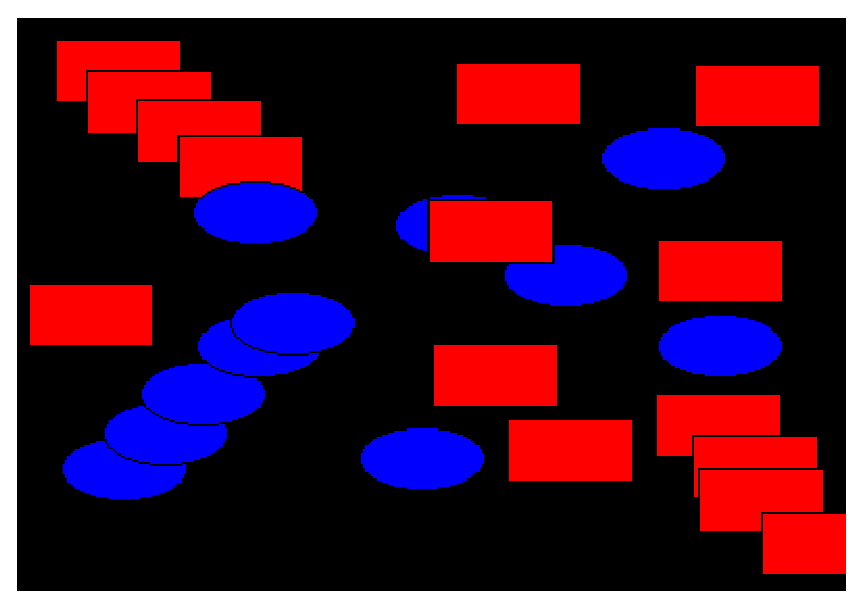
\includegraphics[scale=0.6]{images/simple-stamper.eps}
}



There are several ways to write this example. There could be a separate class to handle
mouse events, as in the previous example.  However, in this case, I decided to let
the panel itself respond to mouse events.  Any object can be a mouse listener, as long
as it implements the \classname{MouseListener} interface.  In this case,
the panel class implements the \classname{MouseListener} interface, 
so the object that represents the main panel of the program can be the mouse
listener for the program.  The constructor for the panel class contains the statement

\displaycode{addMouseListener(this);}\donedisplaycode


\noindent which is equivalent to saying \code{this.addMouseListener(this)}.  Now, the
ordinary way to register a mouse listener is to say \code{X.addMouseListener(Y)}
where \code{Y} is the listener and \code{X} is the component that will
generate the mouse events.  In the statement \code{addMouseListener(this)},
both roles are played by \code{this}; that is, ``this object" (the panel) is
generating mouse events and is also listening for those events.  Although this might
seem a little strange, you should get used to seeing things like this.  In a large
program, however, it's usually a better idea to write a separate class to do
the listening in order to have a more organized division of responsibilities.



The source code for the panel class is shown below.  I have included a \code{main()}
routine to allow the class to be run as a program, as discussed in Subsection~\ref{GUI1.3.7}.
You should check how the instance
methods in the \classname{MouseEvent} object are used. You can also check for the
Four Steps of Event Handling (``\code{import java.awt.event.*}",
``\code{implements MouseListener}",  definitions for the
event-handling methods, and ``\code{addMouseListener}"):

\displaycode{import java.awt.*;
import java.awt.event.*;
import javax.swing.*;

/**
 * A simple demonstration of MouseEvents.  Shapes are drawn
 * on a black background when the user clicks the panel.  If
 * the user Shift-clicks, the panel is cleared.  If the user
 * right-clicks the panel, a blue oval is drawn.  Otherwise,
 * when the user clicks, a red rectangle is drawn.  The contents of
 * the panel are not persistent.  For example, they might disappear 
 * if the panel is resized.
 * This class has a main() routine to allow it to be run as an application.
 */
public class SimpleStamper extends JPanel implements MouseListener \{

    public static void main(String[] args) \{
        JFrame window = new JFrame("Simple Stamper");
        SimpleStamper content = new SimpleStamper();
        window.setContentPane(content);
        window.setDefaultCloseOperation(JFrame.EXIT\_ON\_CLOSE);
        window.setLocation(120,70);
        window.setSize(450,350);
        window.setVisible(true);
    \}

    // ----------------------------------------------------------------------
   
   /**
    * This constructor simply sets the background color of the panel to be black
    * and sets the panel to listen for mouse events on itself.
    */
   public SimpleStamper() \{
      setBackground(Color.BLACK);
      addMouseListener(this);
   \}
   

   /**
    *  Since this panel has been set to listen for mouse events on itself, 
    *  this method will be called when the user clicks the mouse on the panel.
    *  This method is part of the MouseListener interface.
    */
   public void mousePressed(MouseEvent evt) \{
      
      if ( evt.isShiftDown() ) \{
            // The user was holding down the Shift key.  Just repaint the panel.
            // Since this class does not define a paintComponent() method, the 
            // method from the superclass, JPanel, is called.  That method simply
            // fills the panel with its background color, which is black.  The 
            // effect is to clear the panel.
         repaint();
         return;
      \}
      
      int x = evt.getX();  // x-coordinate where user clicked.
      int y = evt.getY();  // y-coordinate where user clicked.
      
      Graphics g = getGraphics(); // Graphics context for drawing directly.
                                  // \newcode{NOTE: This is considered to be bad style!}
      
      if ( evt.isMetaDown() ) \{
             // User right-clicked at the point (x,y). Draw a blue oval centered 
             // at the point (x,y). (A black outline around the oval will make it 
             // more distinct when shapes overlap.)
         g.setColor(Color.BLUE);  // Blue interior.
         g.fillOval( x - 30, y - 15, 60, 30 );
         g.setColor(Color.BLACK); // Black outline.
         g.drawOval( x - 30, y - 15, 60, 30 );
      \}
      else \{
            // User left-clicked (or middle-clicked) at (x,y). 
            // Draw a red rectangle centered at (x,y).
         g.setColor(Color.RED);   // Red interior.
         g.fillRect( x - 30, y - 15, 60, 30 );
         g.setColor(Color.BLACK); // Black outline.
         g.drawRect( x - 30, y - 15, 60, 30 );
      \}
      
      g.dispose();  // We are finished with the graphics context, so dispose of it.
      
   \} // end mousePressed();
   
   
   // The next four empty routines are required by the MouseListener interface.
   // They don't do anything in this class, so their definitions are empty.
   
   public void mouseEntered(MouseEvent evt) \{ \}
   public void mouseExited(MouseEvent evt) \{ \}
   public void mouseClicked(MouseEvent evt) \{ \}
   public void mouseReleased(MouseEvent evt) \{ \}
   
\} // end class SimpleStamper}\donedisplaycode

   
   
\noindent Note, by the way, that this class violates the rule that all
drawing should be done in a \code{paintComponent()} method. The rectangles
and ovals are drawn directly in the \code{mousePressed()} routine. To make
this possible, I need to obtain a graphics context by saying 
``\code{g~=~getGraphics()}". After using \code{g} for drawing, I call
\code{g.dispose()} to inform the operating system that I will no longer be
using \code{g} for drawing.  I do not advise doing this
type of direct drawing if it can be avoided, but you can see that it does work
in this case.




\subsection{MouseMotionListeners and Dragging}\label{GUI1.4.4}



Whenever the mouse is moved, it generates events. The operating system of
the computer detects these events and uses them to move the mouse cursor on the
screen. It is also possible for a program to listen for these ``mouse motion"
events and respond to them. The most common reason to do so is to implement
\newword{dragging}. Dragging occurs when the user moves the
mouse while holding down a mouse button.


The methods for responding to mouse motion events are defined in an
interface named \classname{MouseMotionListener}. This interface specifies two
event-handling methods:

\displaycode{public void mouseDragged(MouseEvent evt);
public void mouseMoved(MouseEvent evt);}\donedisplaycode



The \code{mouseDragged} method is called if the mouse is moved while a
button on the mouse is pressed. If the mouse is moved while no mouse button is
down, then \code{mouseMoved} is called instead. The parameter, \code{evt},
is an object of type \classname{MouseEvent}, which contains the \code{x} and
\code{y} coordinates of the mouse's location, as usual. As long as the user continues
to move the mouse, one of these methods will be called over and over. (So many
events are generated that it would be inefficient for a program to hear them
all, if it doesn't want to do anything in response. This is why the mouse
motion event-handlers are defined in a separate interface from the other mouse
events: You can listen for the mouse events defined in \classname{MouseListener}
without automatically hearing all mouse motion events as well.)


If you want your program to respond to mouse motion events, you must create
an object that implements the \classname{MouseMotionListener} interface, and you
must register that object to listen for events. The registration is done by
calling a component's \code{addMouseMotionListener()} method. The object will
then listen for \code{mouseDragged} and \code{mouseMoved} events associated
with that component. In most cases, the listener object will also implement the
\classname{MouseListener} interface so that it can respond to the other mouse
events as well.


(To get a better idea of how mouse events work, you should try the sample program
\sourceref{SimpleTrackMouse.java}.  This program
responds to any of the seven different kinds of mouse events
by displaying the coordinates of the mouse, the type of event, and a list of
the modifier keys that are down (Shift, Control, Meta, and Alt). 
You can experiment with the program to see what happens as you do various
things with the mouse.  I also encourage you to read the source code. 
You should now be familiar with all the techniques that it uses.)

   

It is interesting to look at what a program needs to do in order to respond
to dragging operations. In general, the response involves three methods:
\code{mousePressed()}, \code{mouseDragged()}, and \code{mouseReleased()}.
The dragging gesture starts when the user presses a mouse button, it continues
while the mouse is dragged, and it ends when the user releases the button. This
means that the programming for the response to one dragging gesture must be
spread out over the three methods! Furthermore, the \code{mouseDragged()}
method can be called many times as the mouse moves. To keep track of what is
going on between one method call and the next, you need to set up some instance
variables. In many applications, for example, in order to process a
\code{mouseDragged} event, you need to remember the previous coordinates of
the mouse. You can store this information in two instance variables
\code{prevX} and \code{prevY} of type \ptype{int}.  It can also
be useful to save the starting coordinates, where the original \code{mousePressed} event
occurred, in instance variables.   And I suggest having a
\ptype{boolean} variable, \code{dragging}, which is set to \code{true}
while a dragging gesture is being processed. This is necessary because in many applications, not
every \code{mousePressed} event starts a dragging operation to which you want to respond. The
\code{mouseDragged} and \code{mouseReleased} methods can use the value of
\code{dragging} to check whether a drag operation is actually in progress.
You might need other instance variables as well, but in general outline, a class
that handles mouse dragging looks like this:

\displaycode{import java.awt.event.*;
   
public class MouseDragHandler implements MouseListener, MouseMotionListener \{

   private int startX, startY; // Point where the original mousePress occurred. 
   private int prevX, prevY;   // Most recently processed mouse coords.
   private boolean dragging;   // Set to true when dragging is in process.
   . . . // other instance variables for use in dragging
   
   public void mousePressed(MouseEvent evt) \{
      if ( \textit{we-want-to-start-dragging} ) \{
          dragging = true;
          startX = evt.getX();  // Remember starting position.
          startY = evt.getY();
          prevX = startX;       // Remember most recent coords.
          prevY = startY;
             . 
             . // Other processing.
             .
      \}
   \}
   
   public void mouseDragged(MouseEvent evt) \{
       if ( dragging == false )  // First, check if we are 
           return;               //   processing a dragging gesture.
       int x = evt.getX(); // Current position of Mouse.
       int y = evt.getY();
         .  
         .  // Process a mouse movement from (prevX, prevY) to (x,y).
         .
       prevX = x;  // Remember the current position for the next call.
       prevY = y;
   \}
   
   public void mouseReleased(MouseEvent evt) \{
       if ( dragging == false )  // First, check if we are 
           return;               //   processing a dragging gesture.
       dragging = false;  // We are done dragging.
        .
        .  // Other processing and clean-up.
        .
   \}

\}}\donedisplaycode




As an example, let's look at a typical use of dragging: allowing the user to
sketch a curve by dragging the mouse. This example also shows many other
features of graphics and mouse processing. In the program, you can
draw a curve by dragging the mouse on a large white drawing area, and you can
select a color for
drawing by clicking on one of several colored rectangles to the right of the
drawing area. The complete source code can be found in \sourceref{SimplePaint.java}.
Here is a picture of the program after some drawing has been done:


\par\dumpfigure{
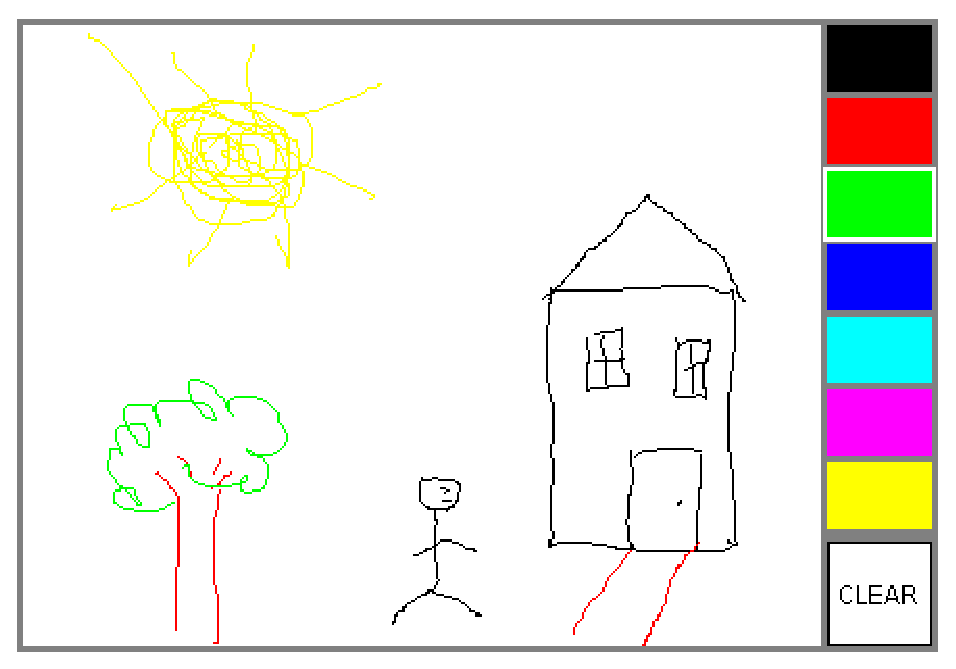
\includegraphics[scale=0.5]{images/simple-paint.eps}
}



I will discuss a few aspects of the source code
here, but I encourage you to read it carefully in its entirety. There are
lots of informative comments in the source code.  


The panel for this example is designed to work for any reasonable
size, that is, unless the panel is too small. This means that
coordinates are computed in terms of the actual width and height of the panel.
(The width and height are obtained by calling \code{getWidth()} and
\code{getHeight()}.) This makes things quite a bit harder than they
would be if we assumed some particular fixed size for the panel. Let's look at
some of these computations in detail. For example, the large white drawing
area extends from \code{y~=~3} to \code{y~=~height~-~3} vertically and
from \code{x~=~3} to \code{x~=~width~-~56} horizontally.  These numbers
are needed in order to interpret the meaning of a mouse click.  They take into
account a gray border around the panel and the color palette along the right
edge of the panel. The gray border is 3 pixels wide.  The colored rectangles are 50
pixels wide.  Together with the 3-pixel border around the panel and 
a 3-pixel divider between the drawing area and the colored
rectangles, this adds up to put the right edge of the drawing area 56
pixels from the right edge of the panel.


A white square labeled ``\code{CLEAR}" occupies a 50-by-50 pixel region
beneath the colored rectangles on the right edge of the panel.
Allowing for this square, we can figure out how
much vertical space is available for the seven colored rectangles, and then
divide that space by 7 to get the vertical space available for each rectangle.
This quantity is represented by a variable, \code{colorSpace}. Out of this
space, 3 pixels are used as spacing between the rectangles, so the height of
each rectangle is \code{colorSpace~-~3}. The top of the \code{N}-th
rectangle is located \code{(N*colorSpace~+~3)} pixels down from the top of
the panel, assuming that we count the rectangles starting with zero. This is because there are
\code{N} rectangles above the \code{N}-th rectangle, each of which uses
\code{colorSpace} pixels. The extra 3 is for the border at the top of the
panel. After all that, we can write down the command for drawing the
\code{N}-th rectangle:

\displaycode{g.fillRect(width - 53, N*colorSpace + 3, 50, colorSpace - 3);}\donedisplaycode

   
\noindent That was not easy! But it shows the kind of careful thinking and precision
graphics that are sometimes necessary to get good results.


The mouse in this program is used to do three different things: Select a
color, clear the drawing, and draw a curve. Only the third of these involves
dragging, so not every mouse click will start a dragging operation. The
\code{mousePressed()} method has to look at the \code{(x,y)} coordinates
where the mouse was clicked and decide how to respond. If the user clicked on
the \code{CLEAR} rectangle, the drawing area is cleared by calling
\code{repaint()}. If the user clicked somewhere in the strip of colored
rectangles, the corresponding color is selected for drawing. This involves computing which color
the user clicked on, which is done by dividing the \code{y} coordinate by
\code{colorSpace}. Finally, if the user clicked on the drawing area, a drag
operation is initiated. In this case, a boolean variable, \code{dragging}, is set to
\code{true} so that the \code{mouseDragged} and \code{mouseReleased}
methods will know that a curve is being drawn. The code for this follows the
general form given above. The actual drawing of the curve is done in the
\code{mouseDragged()} method, which draws a line from the previous location of
the mouse to its current location. Some effort is required to make sure that
the line does not extend beyond the white drawing area of the panel. This is
not automatic, since as far as the computer is concerned, the border and the
color bar are part of the drawing surface. If the user drags the mouse outside
the drawing area while drawing a line, the \code{mouseDragged()} routine
changes the \code{x} and \code{y} coordinates to make them lie within the
drawing area.


   
\subsection[Anonymous Event Handlers]{Anonymous Event Handlers and Adapter Classes}\label{GUI1.4.5}



As I mentioned above, it is a fairly common practice to use anonymous inner
classes to define listener objects. As discussed in Subsection~\ref{OOP.8.3},
a special form of the \code{new} operator is
used to create an object that belongs to an anonymous class. For example, a
mouse listener object can be created with an expression of the form:

\displaycode{new MouseListener() \{
   public void mousePressed(MouseEvent evt) \{ . . . \}
   public void mouseReleased(MouseEvent evt) \{ . . . \}
   public void mouseClicked(MouseEvent evt) \{ . . . \}
   public void mouseEntered(MouseEvent evt) \{ . . . \}
   public void mouseExited(MouseEvent evt) \{ . . . \}
\}}\donedisplaycode


\noindent This is all just one long expression that both defines an unnamed class and
creates an object that belongs to that class. To use the object as a mouse
listener, it can be passed as the parameter to some component's
\code{addMouseListener()} method in a command of the form:

\displaycode{\newcode{component.addMouseListener(} new MouseListener() \{
      public void mousePressed(MouseEvent evt) \{ . . . \}
      public void mouseReleased(MouseEvent evt) \{ . . . \}
      public void mouseClicked(MouseEvent evt) \{ . . . \}
      public void mouseEntered(MouseEvent evt) \{ . . . \}
      public void mouseExited(MouseEvent evt) \{ . . . \}
   \} \newcode{);}}\donedisplaycode



Now, in a typical application, most of the method definitions in this class
will be empty. A class that implements an \code{interface} must provide
definitions for all the methods in that interface, even if the definitions are
empty. To avoid the tedium of writing empty method definitions in cases like
this, Java provides \newword{adapter classes}. An adapter
class implements a listener interface by providing empty definitions for all
the methods in the interface. An adapter class is useful only as a basis for
making subclasses. In the subclass, you can define just those methods that you
actually want to use. For the remaining methods, the empty definitions that are
provided by the adapter class will be used. The adapter class \classname{MouseAdapter}
implements both the \classname{MouseListener} interface and the
\classname{MouseMotionListener} interface, so it can be used as a basis for
creating a listener for any mouse event.  As an example,
if you want a mouse listener that only responds to mouse-pressed events, you
can use a command of the form:

\displaycode{component.addMouseListener( new \newcode{MouseAdapter()} \{
      public void mousePressed(MouseEvent evt) \{ . . . \}
   \} );}\donedisplaycode


\noindent To see how this works in a real example, let's write another version of the
\classname{ClickableRandomStrings} program from Subsection~\ref{GUI1.4.2}.
This version uses an anonymous class based on
\classname{MouseAdapter} to handle mouse events:

\displaycode{import java.awt.Component;
import java.awt.event.MouseAdapter;
import java.awt.event.MouseEvent;
import java.awt.event.MouseListener;
import javax.swing.JFrame;

public class ClickableRandomStrings2 \{
   
   public static void main(String[] args) \{
      JFrame window = new JFrame("Random Strings");
      RandomStringsPanel content = new RandomStringsPanel();

      \newcode{content.addMouseListener( new MouseAdapter() \{ 
            // Register a mouse listener that is defined by an anonymous subclass
            // of MouseAdapter.  This replaces the RepaintOnClick class that was
            // used in the original version.
         public void mousePressed(MouseEvent evt) \{
            Component source = (Component)evt.getSource();
            source.repaint();
         \}
      \} );}

      window.setContentPane(content);
      window.setDefaultCloseOperation(JFrame.EXIT\_ON\_CLOSE);
      window.setLocation(100,75);
      window.setSize(300,240);
      window.setVisible(true);
   \}

\}}\donedisplaycode

   

Anonymous inner classes can be used for other purposes besides event handling.
For example, suppose that you want to define a subclass of \classname{JPanel}
to represent a drawing surface.  The subclass will only be used once.  It will redefine
the \code{paintComponent()} method, but will make no other changes to
\classname{JPanel}.  It might make sense to define the subclass as
an anonymous inner class.  You will see this pattern used in some future examples.


   

   



\section{Timers, KeyEvents, and State Machines}\label{GUI1.5}

   

\start{{\Large N}ot every event} is generated by an action on the
part of the user.  Events can also be generated by objects as part of their
regular programming, and these events can be monitored by other objects so that
they can take appropriate actions when the events occur.  One example of this
is the class \code{javax.swing.Timer}.  A \classname{Timer}
generates events at regular intervals.  These events can be used to drive
an animation or to perform some other task at regular intervals.  We will
begin this section with a look at timer events and animation.  We will then
look at another type of basic user-generated event:  the \classname{KeyEvents}
that are generated when the user types on the keyboard.  The example at the end
of the section uses both a timer and keyboard events to implement a simple game
and introduces the important idea of \newword{state machines}.

\subsection{Timers and Animation}\label{GUI1.5.1}

   

An object belonging to the class \code{javax.swing.Timer} exists only to
generate events.  A \classname{Timer}, by default, generates a sequence of events
with a fixed delay between each event and the next.  (It is also possible to set a
\classname{Timer} to emit a single event after a specified time delay;
in that case, the timer is being used as an ``alarm.")  Each event belongs to the
class \classname{ActionEvent}.  An object that is to listen for the
events must implement the interface \classname{ActionListener}, which
defines just one method:
   
\displaycode{public void actionPerformed(ActionEvent evt)}\donedisplaycode

   
\noindent To use a \classname{Timer}, you must create an object that
implements the \classname{ActionListener} interface.  That is, the
object must belong to a class that is declared to ``\code{implement ActionListener}",
and that class must define the \code{actionPerformed} method.  Then, if
the object is set to listen for events from the timer, the code in the listener's
\code{actionPerformed} method will be executed every time the timer generates
an event.
   

Since there is no point to having a timer without having a listener to respond to
its events, the action listener for a timer is specified as a parameter in the
timer's constructor.  The time delay between timer events is also specified in
the constructor.  If \code{timer} is a variable of type \classname{Timer},
then the statement
   
\displaycode{timer = new Timer( millisDelay, listener );}\donedisplaycode

   
\noindent creates a timer with a delay of \code{millisDelay} milliseconds
between events (where 1000 milliseconds equal one second).  Events from the
timer are sent to the \code{listener}.  (\code{millisDelay} must be
of type \ptype{int}, and \code{listener} must be of type
\classname{ActionListener}.)  The listener's \code{actionPerfomed()}
will be executed every time the timer emits an event.
Note that a timer is not guaranteed 
to deliver events at precisely regular intervals.  If the computer is busy
with some other task, an event might be delayed or even dropped altogether.
   

A timer does not automatically start generating events when the timer object
is created.  The \code{start()} method in the timer must be called to tell
the timer to start running.  The timer's \code{stop()} method
can be used to turn the stream of events off. It can be restarted later by calling
\code{start()} again.

   

\mybreak

   

One application of timers is computer animation.
A computer animation is just a sequence of still images, presented to the user
one after the other.  If the time between images is short, and if the change from one
image to another is not too great, then the user perceives continuous motion.
The easiest way to do animation in Java is to use a \classname{Timer} to
drive the animation.  Each time the timer generates an event, the next frame of
the animation is computed and drawn on the screen---the code that implements this goes
in the \code{actionPerformed} method of an object that listens for events from
the timer.


Our first example of using a timer is not exactly an animation, but it does
display a new image for each timer event.  The program shows randomly generated
images that vaguely resemble works of abstract art.  In fact, the program
draws a new random image every time its \code{paintComponent()} method is
called, and the response to a timer event is simply to call \code{repaint()},
which in turn triggers a call to \code{paintComponent}.  The work
of the program is done in a subclass of \classname{JPanel}, which
starts like this:
   
\displaycode{import java.awt.*;
import java.awt.event.*;
import javax.swing.*;

public class RandomArtPanel extends JPanel \{
   
   /**
    * A RepaintAction object calls the repaint method of this panel each
    * time its actionPerformed() method is called.  An object of this
    * type is used as an action listener for a Timer that generates an
    * ActionEvent every four seconds.  The result is that the panel is
    * redrawn every four seconds.
    */
   private class RepaintAction implements ActionListener \{
      public void actionPerformed(ActionEvent evt) \{
         repaint();  // Call the repaint() method in the panel class.
      \}
   \}
   
   /**
    * The constructor creates a timer with a delay time of four seconds
    * (4000 milliseconds), and with a RepaintAction object as its
    * ActionListener.  It also starts the timer running.
    */
   public RandomArtPanel() \{
      RepaintAction action = new RepaintAction();
      Timer timer = new Timer(4000, action);
      timer.start();
   \}
   
   /**
    * The paintComponent() method fills the panel with a random shade of
    * gray and then draws one of three types of random "art".  The type
    * of art to be drawn is chosen at random.
    */
   public void paintComponent(Graphics g) \{
       .
       .   // The rest of the class is omitted
       .}\donedisplaycode

   
\noindent You can find the full source code for this class in the file \sourceref{RandomArt.java}.
I will only note that the very short \classname{RepaintAction} class is a natural 
candidate to be replaced by an anonymous inner class. That can be done where the timer is
created:


\displaycode{Timer timer = new timer(4000, new ActionListener() \{
        public void actionPerformed(ActionEvent evt) \{
            repaint();
        \}
    \});
}\donedisplaycode

   
   
\noindent Later in this section, we will use a timer to drive the animation in a simple
computer game.
   

   
\subsection{Keyboard Events}\label{GUI1.5.2}



In Java, user actions become events in a program. These events
are associated with GUI components.
When the user presses a button on the mouse, the event that is generated is
associated with the component that contains the mouse cursor. What about
keyboard events? When the user presses a key, what component is associated with
the key event that is generated?


A GUI uses the idea of \newword{input focus} to determine
the component associated with keyboard events. At any given time, exactly one
interface element on the screen has the input focus, and that is where all
keyboard events are directed. If the interface element happens to be a Java
component, then the information about the keyboard event becomes a Java object
of type \classname{KeyEvent}, and it is delivered to any listener objects that are
listening for \code{KeyEvents} associated with that component. The necessity
of managing input focus adds an extra twist to working with keyboard events.


It's a good idea to give the user some visual feedback about which component
has the input focus. For example, if the component is the typing area of a
word-processor, the feedback is usually in the form of a blinking text cursor.
Another possible visual clue is to draw a brightly colored border around the edge
of a component when it has the input focus, as I do in the examples given
later in this section.


If \code{comp} is any component, and you would like it to have the
input focus, you can call \code{requestFocusInWindow()}, which should
work as long as the window that contains the component is active and there 
is only one component that is requesting focus.  In some cases,
when there is only one component involved, it is enough to call this method
once, just after opening the window, and the component will retain the focus
for the rest of the program.  (Note that there is also a \code{requestFocus()}
method that might work even when the window is not active, 
but the newer method \code{requestFocusInWindow()} is preferred in
most cases.)


In a typical user interface, the user can choose to give the focus to a component by
clicking on that component with the mouse. And pressing the tab key will often
move the focus from one component to another.  This is handled automatically by
the components involved, without any programming on your part.
However, some components do not automatically request the input focus when the user
clicks on them. To solve this problem, a program can register a mouse
listener with the component to detect user clicks. In response to a user click,
the \code{mousePressed()} method should call \code{requestFocusInWindow()} for the
component. This is true, in particular, for \classname{JPanels} that are used as
drawing surfaces, since \classname{JPanel} objects do not receive the input
focus automatically.


As our first example of processing key events, we look at a simple program in
which the user moves a square up, down, left, and right by pressing arrow keys.
When the user hits the 'R', 'G', 'B', or 'K' key, the color of the square is set to
red, green, blue, or black, respectively.  Of course, none of these key events
are delivered to the panel unless it has the input focus.  The panel in the
program changes its appearance when it has the input focus:  When it does,
a cyan-colored border is drawn around the panel; when it does not, a gray-colored
border is drawn.  The complete source code for this example
can be found in the file \sourceref{KeyboardAndFocusDemo.java}. 
I will discuss some aspects of it below. After reading this section, you should be
able to understand the source code in its entirety.  I suggest running the program to
see how it works.



In Java, keyboard event objects belong to a class called \classname{KeyEvent}.
An object that needs to listen for \classname{KeyEvents} must implement the
interface named \classname{KeyListener}. Furthermore, the object must be
registered with a component by calling the component's
\code{addKeyListener()} method. The registration is done with the command
``\code{component.addKeyListener(listener);}" where \code{listener} is the
object that is to listen for key events, and \code{component} is the object
that will generate the key events (when it has the input focus). It is possible
for \code{component} and \code{listener} to be the same object. All this
is, of course, directly analogous to what you learned about mouse events in the
previous section. The \classname{KeyListener} interface
defines the following methods, which must be included in any class that
implements \classname{KeyListener}:

\displaycode{public void keyPressed(KeyEvent evt);
public void keyReleased(KeyEvent evt);
public void keyTyped(KeyEvent evt);}\donedisplaycode



Java makes a careful distinction between \textit{the keys that you press} and
\textit{the characters that you type}. There are lots of keys on a keyboard:
letter keys, number keys, modifier keys such as Control and Shift, arrow keys,
page up and page down keys, keypad keys, function keys, and so on. In some cases, such as the shift key,
pressing a key does not type a character. On the other hand, typing a character
sometimes involves pressing several keys. For example, to type an uppercase
'A', you have to press the Shift key and then press the A key before releasing
the Shift key. On my Mac~OS computer, I can type an accented e, by
holding down the Option key, pressing the E key, releasing the Option key, and
pressing E again. Only one character was typed, but I had to perform three
key-presses and I had to release a key at the right time. In Java, there are
three types of \classname{KeyEvent}. The types correspond to pressing a key,
releasing a key, and typing a character. The \code{keyPressed} method is
called when the user presses a key, the \code{keyReleased} method is called
when the user releases a key, and the \code{keyTyped} method is called when
the user types a character (whether that's done with one key press or several).
Note that one user action, such as pressing the E
key, can be responsible for two events, a \code{keyPressed} event and a
\code{keyTyped} event. Typing an upper case 'A' can generate two
\code{keyPressed} events, two \code{keyReleased} events, and one \code{keyTyped}
event.


Usually, it is better to think in terms of two separate streams of events,
one consisting of \code{keyPressed} and \code{keyReleased} events and the
other consisting of \code{keyTyped} events. For some applications, you want
to monitor the first stream; for other applications, you want to monitor the
second one. Of course, the information in the \code{keyTyped} stream could be
extracted from the \code{keyPressed/keyReleased} stream, but it would be
difficult (and also system-dependent to some extent). Some user actions, such
as pressing the Shift key, can only be detected as \code{keyPressed} events.
I used to have a computer solitaire game that highlighted every card that could be
moved, when I held down the Shift key. You can do something like that in Java
by hiliting the cards when the Shift key is pressed and removing the highlight
when the Shift key is released.


There is one more complication. Usually, when you hold down a key on the
keyboard, that key will \newword{auto-repeat}. This means
that it will generate multiple \code{keyPressed} events with just one
\code{keyReleased} at the end of the sequence. 
It can also generate multiple \code{keyTyped} events. For the most
part, this will not affect your programming, but you should not expect every
\code{keyPressed} event to have a corresponding \code{keyReleased}
event.


Every key on the keyboard has an integer code number. (Actually, this is
only true for keys that Java knows about. Many keyboards have extra keys that
can't be used with Java.) When the \code{keyPressed} or \code{keyReleased}
method is called, the parameter, \code{evt}, contains the code of the key
that was pressed or released. The code can be obtained by calling the function
\code{evt.getKeyCode()}. Rather than asking you to memorize a table of code
numbers, Java
provides a named constant for each key. These constants are defined in the
\classname{KeyEvent} class. For example the constant for the shift key is
\code{KeyEvent.VK\_SHIFT}. If you want to test whether the key that the user
pressed is the Shift key, you could say ``\code{if (evt.getKeyCode() ==
KeyEvent.VK\_SHIFT)}". The key codes for the four arrow keys are
\code{KeyEvent.VK\_LEFT}, \code{KeyEvent.VK\_RIGHT}, \code{KeyEvent.VK\_UP},
and \code{KeyEvent.VK\_DOWN}. Other keys have similar codes. (The ``VK" stands
for ``Virtual Keyboard". In reality, different keyboards use different key
codes, but Java translates the actual codes from the keyboard into its own
``virtual" codes. Your program only sees these virtual key codes, so it will
work with various keyboards on various platforms without modification.)


In the case of a \code{keyTyped} event, you want to know which character
was typed. This information can be obtained from the parameter, \code{evt},
in the \code{keyTyped} method by calling the function
\code{evt.getKeyChar()}. This function returns a value of type \ptype{char}
representing the character that was typed.


In the \code{KeyboardAndFocusDemo} program, I use the
\code{keyPressed} routine to respond when the user presses one of the arrow
keys. The program includes instance variables, \code{squareLeft} and
\code{squareTop}, that give the position of the upper left corner of the movable
square. When the user presses one of the arrow keys, the \code{keyPressed}
routine modifies the appropriate instance variable and calls
\code{repaint()} to redraw the panel with the square in its new position. Note that the
values of \code{squareLeft} and \code{squareTop} are restricted so that
the square never moves outside the white area of the panel:

\displaycode{/**
 * This is called each time the user presses a key while the panel has
 * the input focus.  If the key pressed was one of the arrow keys,
 * the square is moved (except that it is not allowed to move off the
 * edge of the panel, allowing for a 3-pixel border).
 */
public void keyPressed(KeyEvent evt) \{ 
   
   int key = evt.getKeyCode();  // keyboard code for the pressed key
   
   if (key == KeyEvent.VK\_LEFT) \{  // left-arrow key; move the square left
      squareLeft -= 8;
      if (squareLeft \< 3)
         squareLeft = 3;
      repaint();
   \}
   else if (key == KeyEvent.VK\_RIGHT) \{  // right-arrow key; move the square right
      squareLeft += 8;
      if (squareLeft \> getWidth() - 3 - SQUARE\_SIZE)
         squareLeft = getWidth() - 3 - SQUARE\_SIZE;
      repaint();
   \}
   else if (key == KeyEvent.VK\_UP) \{  // up-arrow key; move the square up
      squareTop -= 8;
      if (squareTop \< 3)
         squareTop = 3;
      repaint();
   \}
   else if (key == KeyEvent.VK\_DOWN) \{  // down-arrow key; move the square down
      squareTop += 8;
      if (squareTop \> getHeight() - 3 - SQUARE\_SIZE)
         squareTop = getHeight() - 3 - SQUARE\_SIZE;
      repaint();
   \}
   
\}  // end keyPressed()}\donedisplaycode



Color changes---which happen when the user types the characters 'R', 'G',
'B', and 'K', or the lower case equivalents---are handled in the
\code{keyTyped} method. I won't include it here, since it is so similar to
the \code{keyPressed} method. Finally, to complete the \classname{KeyListener}
interface, the \code{keyReleased} method must be defined. In the sample
program, the body of this method is empty since the program does nothing in
response to \code{keyReleased} events.


   
\subsection{Focus Events}\label{GUI1.5.3}



If a component is to change its appearance when it has the input focus, it
needs some way to know when it has the focus. In Java, objects are notified
about changes of input focus by events of type \classname{FocusEvent}. An object
that wants to be notified of changes in focus can implement the
\classname{FocusListener} interface. This interface declares two methods:

\displaycode{public void focusGained(FocusEvent evt);
public void focusLost(FocusEvent evt);}\donedisplaycode



Furthermore, the \code{addFocusListener()} method must be used to set up a
listener for the focus events. When a component gets the input focus, it calls
the \code{focusGained()} method of any registered with 
\classname{FocusListener}. When it loses the focus, it calls
the listener's \code{focusLost()} method.


In the sample \code{KeyboardAndFocusDemo} program,  the response to
a focus event is simply to redraw the panel.  The \code{paintComponent()}
method checks whether the panel has the input focus by calling the
\ptype{boolean}-valued function \code{hasFocus()}, which is
defined in the \classname{Component} class, and it draws a
different picture depending on whether or not the panel has the input focus.
The net result is that the appearance of the panel changes when the panel
gains or loses focus.  The methods from the \classname{FocusListener}
interface are defined simply as:

\displaycode{public void focusGained(FocusEvent evt) \{
       // The panel now has the input focus.
   repaint();  // will redraw with a new message and a cyan border
\}
 
public void focusLost(FocusEvent evt) \{
      // The panel has now lost the input focus.
   repaint();  // will redraw with a new message and a gray border
\}}\donedisplaycode



The other aspect of handling focus is to make sure that the panel
actually gets the focus.  In this case, I called \code{requestFocusInWindow()}
for the panel in the program's \code{main()} routine, just after 
opening the window.  This approach works because there is only one component
in the window, and it should have focus as long as the window is active.
If the user clicks over to another window while using the program, the 
window becomes inactive and the panel loses focus temporarily, but gets
is back when the user clicks back to the program window.


There are still decisions to be made about the overall structure of
the program.  In this case, I decided to use a nested class named \classname{Listener} to define
an object that listens for both focus and key events.  In the constructor for the panel, I create
an object of type \classname{Listener} and register it to listen for both
key events and focus events from the panel.  See the \sourceref{source code}
for full details.


   
\subsection{State Machines}\label{GUI1.5.4}



The information stored in an object's instance variables is said to
represent the \newword{state} of that object. When one of
the object's methods is called, the action taken by the object can depend on
its state. (Or, in the terminology we have been using, the definition of the
method can look at the instance variables to decide what to do.) Furthermore,
the state can change. (That is, the definition of the method can assign new
values to the instance variables.) In computer science, there is the idea of a
\newword{state machine}, which is just something that has a
state and can change state in response to events or inputs. The response of a
state machine to an event depends on what state it's in when the event occurs. An object is
a kind of state machine. Sometimes, this point of view can be very useful in
designing classes.


The state machine point of view can be especially useful in the type of
event-oriented programming that is required by graphical user interfaces. When
designing a GUI program, you can ask yourself: What information about state do I
need to keep track of? What events can change the state of the program? How will
my response to a given event depend on the current state? Should the appearance
of the GUI be changed to reflect a change in state? How should the
\code{paintComponent()} method take the state into account? All this is an
alternative to the top-down, step-wise-refinement style of program design,
which does not apply to the overall design of an event-oriented program.


In the \classname{KeyboardAndFocusDemo} program, shown above, the state of the
program is recorded in the instance variables \code{squareColor},
\code{squareLeft}, and \code{squareTop}. These state variables are used in
the \code{paintComponent()} method to decide how to draw the panel. Their values are
changed in the two key-event-handling methods.


In the rest of this section, we'll look at another example, where the state
plays an even bigger role. In this example, the user plays a
simple arcade-style game by pressing the arrow keys.  The
program is defined in the source code file \sourceref{SubKiller.java}.
As usual, it would be a good idea to compile and run the program as well
as read the full source code.  Here is a picture:


\par\dumpfigure{
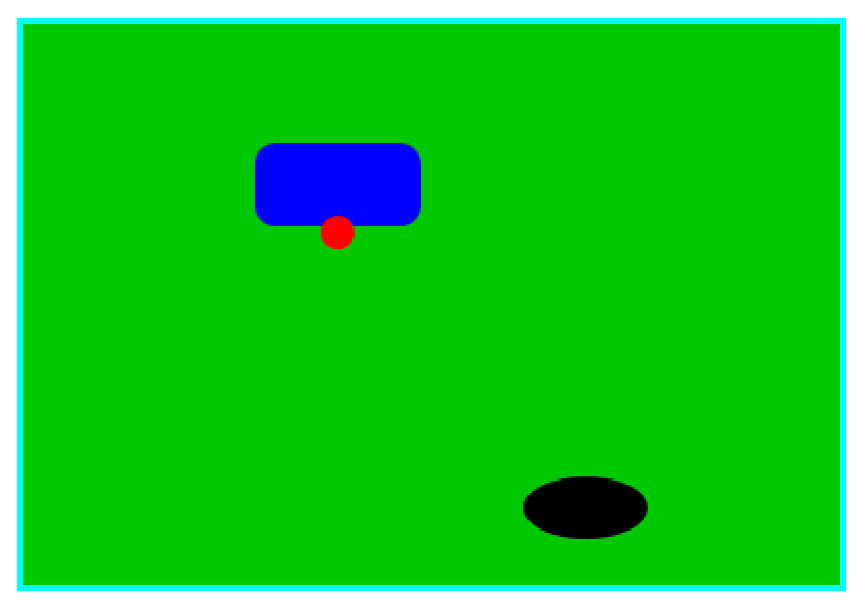
\includegraphics[scale=0.5]{images/sub-killer.eps}
}



The program shows a black ``submarine" near the bottom of the panel.
While the panel has the input focus, this submarine
moves back and forth erratically near the bottom. Near the top,
there is a blue ``boat." You can move this boat back and forth by pressing the
left and right arrow keys. Attached to the boat is a red ``bomb" (or ``depth charge"). You
can drop the bomb by hitting the down arrow key. The objective is to
blow up the submarine by hitting it with the bomb. If the bomb
falls off the bottom of the screen, you get a new one. If the submarine explodes, a
new sub is created and you get a new bomb. Try it! Make sure to hit the
sub at least once, so you can see the explosion.


Let's think about how this game can be programmed. First of all, since we
are doing object-oriented programming, I decided to represent the boat, the depth
charge, and the submarine as objects.  Each of these objects is defined by a
separate nested class inside the main panel class, and each object has its own
state which is represented by the instance variables in the corresponding class.
I use variables \code{boat}, \code{bomb}, and \code{sub} in
the panel class to refer to the boat, bomb, and submarine objects.


Now, what constitutes the
``state" of the program? That is, what things change from time to time and affect
the appearance or behavior of the program? Of course, the state includes the
positions of the boat, submarine, and bomb, so those objects have instance
variables to store the positions.  Anything else, possibly less obvious? Well,
sometimes the bomb is falling, and sometimes it's not. That is a
difference in state. Since there are two possibilities, I represent this aspect
of the state with a boolean variable in the \code{bomb} object, 
\code{bomb.isFalling}. Sometimes the
submarine is moving left and sometimes it is moving right. The difference is
represented by another boolean variable, \code{sub.isMovingLeft}. Sometimes,
the sub is exploding. This is also part of the state, and it  is represented
by a boolean variable, \code{sub.isExploding}.  However, the explosions
require a little more thought.   An explosion is something that takes place
over a series of frames.  While an explosion is in progress, the sub
looks different in each frame, as the size of the explosion increases. Also,
I need to know when the explosion is over so that I can go back to moving and drawing the
sub as usual. So, I use an integer variable, \code{sub.explosionFrameNumber}
to record how many frames have been drawn since the explosion
started; the value of this variable is used only when an explosion is in progress.


How and when do the values of these state variables change?  Some of them seem
to change on their own:  For example, as the sub moves left and right, the state variables
that specify its position change.  Of course, these variables are changing
because of an animation, and that animation is driven by a timer.  Each time an
event is generated by the timer, some of the state variables have to change to
get ready for the next frame of the animation.  The changes are made by the
action listener that listens for events from the timer.  The \code{boat},
\code{bomb}, and \code{sub} objects each contain an
\code{updateForNextFrame()} method that updates the state variables of
the object to get ready for the next frame of the animation.  The action listener
for the timer calls these methods with the statements
   
\displaycode{boat.updateForNewFrame();
bomb.updateForNewFrame();
sub.updateForNewFrame();}\donedisplaycode


\noindent The action listener also calls \code{repaint()}, so that the panel will be
redrawn to reflect its new state.  There are several state variables that change
in these update methods, in addition to the position of the sub:  If the bomb is
falling, then its y-coordinate increases from one frame to the next.  If the
bomb hits the sub, then the \code{isExploding} variable of the sub
changes to true, and the \code{isFalling} variable of the bomb becomes \code{false}.
The \code{isFalling} variable also becomes false when the bomb falls off the
bottom of the screen.  If the sub is exploding, then its \code{explosionFrameNumber}
increases from one frame to the next, and when it reaches a certain value, the
explosion ends and \code{isExploding} is reset to false.  At random times,
the sub switches between moving to the left and moving to the right.  Its
direction of motion is recorded in the sub's \code{isMovingLeft} variable.
The sub's \code{updateForNewFrame()} method includes these lines to
change the value of \code{isMovingLeft} at random times:
   
\displaycode{if ( Math.random() \< 0.04 )
   isMovingLeft = ! isMovingLeft;}\donedisplaycode


\noindent There is a 1 in 25 chance that \code{Math.random()} will be less than
0.04, so the statement ``\code{isMovingLeft = !~isMovingLeft}" is executed
in one in every twenty-five frames, on average.  The effect of this statement
is to reverse the value of \code{isMovingLeft}, from false to true or from
true to false.  That is, the direction of motion of the sub is reversed.
      

In addition to changes in state that take place from one frame to the next, a few state
variables change when the user presses certain keys. In the program, this is checked
in a method that responds to user keystrokes. If the user presses the left or right
arrow key, the position of the boat is changed. If the user presses the down
arrow key, the bomb changes from not-falling to falling. This is coded in the
\code{keyPressed()}method of a \classname{KeyListener} that is
registered to listen for key events on the panel; that method 
reads as follows:

\displaycode{public void keyPressed(KeyEvent evt) \{
   int code = evt.getKeyCode();  // which key was pressed.
   if (code == KeyEvent.VK\_LEFT) \{
        // Move the boat left.  (If this moves the boat out of the frame, its
        // position will be adjusted in the boat.updateForNewFrame() method.)
      boat.centerX -= 15;
   \}
   else if (code == KeyEvent.VK\_RIGHT) \{  
        // Move the boat right.  (If this moves boat out of the frame, its
        // position will be adjusted in the boat.updateForNewFrame() method.)
      boat.centerX += 15;
   \}
   else if (code == KeyEvent.VK\_DOWN) \{
         // Start the bomb falling, if it is not already falling.
      if ( bomb.isFalling == false )
         bomb.isFalling = true;
   \}
\}}\donedisplaycode


\noindent Note that it's not necessary to call \code{repaint()} in this method,
since this panel shows an animation that is constantly being redrawn
anyway. Any changes in the state will become visible to the user as soon as the
next frame is drawn. At some point in the program, I have to make sure that the
user does not move the boat off the screen. I could have done this in
\code{keyPressed()}, but I choose to check for this in another routine, in
the boat object.


The program uses four listeners, to respond to
action events from the timer, key events from the user, focus events, and
mouse events.  In this program, the user must click the panel to start the game.
The game is programmed to run as long as the panel has the input focus.
In this example, the program does not automatically request the focus; the user
has to do it.  When the user clicks the panel, the mouse listener requests the input focus and the
game begins.  The timer runs only when the panel has the input focus; this
is programmed by having the focus listener start the timer when the panel
gains the input focus and stop the timer when the panel loses the input focus.
All four listeners are created in the constructor of the \classname{SubKillerPanel}
class using anonymous inner classes.  (See Subsection~\ref{GUI1.4.5}.)


I encourage you to read the source code in \sourceref{SubKiller.java}.
Although a few points are tricky, you should  with some effort be able to read and
understand the entire program.  Try to understand the program in terms of state
machines.  Note how the state of each of the three objects in the program changes
in response to events from the timer and from the user.
   

While it's not at all sophisticated as arcade games go, the
SubKiller game does use some interesting programming. And it
nicely illustrates how to apply state-machine thinking in event-oriented
programming.
   

 

   



\section{Basic Components}\label{GUI1.6}

   

\start{{\Large I}n preceding sections}, you've seen how to use a
graphics context to draw on the screen and how to handle mouse events and
keyboard events. In one sense, that's all there is to GUI programming. If
you're willing to program all the drawing and handle all the mouse and keyboard
events, you have nothing more to learn. However, you would either be doing a
lot more work than you need to do, or you would be limiting yourself to very
simple user interfaces. A typical user interface uses standard GUI components
such as buttons, scroll bars, text-input boxes, and menus. These components
have already been written for you, so you don't have to duplicate the work
involved in developing them. They know how to draw themselves, and they can
handle the details of processing the mouse and keyboard events that concern
them.


Consider one of the simplest user interface components, a push button. The
button has a border, and it displays some text. This text can be changed.
Sometimes the button is disabled, so that clicking on it doesn't have any
effect. When it is disabled, its appearance changes. When the user clicks on
the push button, the button changes appearance while the mouse button is
pressed and changes back when the mouse button is released. In fact, it's more
complicated than that. If the user moves the mouse outside the push button
before releasing the mouse button, the button changes to its regular
appearance. To implement this, it is necessary to respond to mouse exit or
mouse drag events. Furthermore, on many platforms, a button can receive the
input focus. The button changes appearance when it has the focus. If the button
has the focus and the user presses the space bar, the button is triggered. This
means that the button must respond to keyboard and focus events as well.


Fortunately, you don't have to program \textbf{any} of this, provided you
use an object belonging to the standard class \code{javax.swing.JButton}. A
\classname{JButton} object draws itself and processes mouse, keyboard, and focus
events on its own. You only hear from the \classname{JButton} when the user
triggers it by clicking on it or pressing the space bar while the button has
the input focus. When this happens, the \classname{JButton} object creates an
event object belonging to the class \code{java.awt.event.ActionEvent}. The
event object is sent to any registered listeners to tell them that the button
has been pushed. Your program gets only the information it needs---the fact
that a button was pushed.
   

\mybreak

   

The standard components that are defined as part of the Swing graphical user interface
API are defined by subclasses of the class \classname{JComponent}, which is 
itself a subclass of \classname{Component}.  (Note that this includes the
\classname{JPanel} class that we have already been working with extensively.)
Many useful methods are
defined in the \classname{Component} and \classname{JComponent}
classes and so can be used with any Swing component.  We begin by looking at a
few of these methods.  Suppose that \code{comp} is a variable that refers
to some \classname{JComponent}.  Then the following methods can be
used:



\mylist{

\myitem \codedef{comp.getWidth()} and \codedef{comp.getHeight()} are functions that
give the current size of the component, in pixels.  One warning: When a component is first
created, its size is zero. The size will be set later, probably by a layout
manager. A common mistake is to check the size of a component before that size
has been set, such as in a constructor.
\myitem \codedef{comp.setEnabled(true)} and
\codedef{comp.setEnabled(false)} can be used to
enable and disable the component. When a component is disabled, its appearance
might change, and the user cannot do anything with it.  There is a boolean-valued
function, \codedef{comp.isEnabled()} that you can
call to discover whether the component is enabled.
\myitem \codedef{comp.setVisible(true)} and
\codedef{comp.setVisible(false)} can be called to
hide or show the component.
\myitem \codedef{comp.setFont(font)} sets the font that
is used for text displayed on the component. See Subsection~\ref{GUI1.3.3}
for a discussion of fonts.
\myitem \codedef{comp.setBackground(color)} and
\codedef{comp.setForeground(color)} set the
background and foreground colors for the component.  See Subsection~\ref{GUI1.3.2}.
\myitem \codedef{comp.setOpaque(true)} tells the
component that the area occupied by the component should be filled with the
component's background color before the content of the component is painted. By
default, only \classname{JLabels} are non-opaque. A non-opaque,
or ``transparent", component ignores its background color and simply paints its
content over the content of its container. This usually means that it inherits
the background color from its container.
\myitem \codedef{comp.setToolTipText(string)} sets the
specified string as a ``tool tip" for the component. The tool tip is displayed
if the mouse cursor is in the component and the mouse is not moved for a few
seconds. The tool tip should give some information about the meaning of the
component or how to use it.
\myitem \codedef{comp.setPreferredSize(size)} sets the
size at which the component should be displayed, if possible. The parameter is
of type \code{java.awt.Dimension}, where an object of type \classname{Dimension}
has two public integer-valued instance variables, \code{width} and \code{height}.
A call to this method usually looks something
like ``\code{setPreferredSize( new Dimension(100,50)~)}". The preferred
size is used as a hint by layout managers, but will not be respected in all
cases.  Standard components generally compute a correct
preferred size automatically, but it can be useful to set it in some cases. For
example, if you use a \classname{JPanel} as a drawing surface, it is usually a good
idea to set a preferred size for it, since its default preferred size is zero.
}


   

Note that using
any component is a multi-step process. The component object must be created
with a constructor. It must be added to a container. In many cases, a listener
must be registered to respond to events from the component. And in some cases,
a reference to the component must be saved in an instance variable so that the
component can be manipulated by the program after it has been created.
In this section, we will look at a few of the basic standard components that are
available in Swing. In the next section
we will consider the problem of laying out components in containers.

   
\subsection{JButton}\label{GUI1.6.1}

   

An object of class \classname{JButton} is a push button that the user
can click to trigger some action. You've already seen
buttons used in Section~\ref{GUI1.1}, but we consider
them in much more detail here.  To use any component effectively, there are several
aspects of the corresponding class that you should be familiar with.  For
\classname{JButton}, as an example, I list these aspects explicitly:



\mylist{

\myitem \textbf{Constructors}: The \classname{JButton} class has a constructor that
takes a string as a parameter. This string becomes the text displayed on the
button. For example: \code{stopGoButton = new~JButton("Go")}.  This creates
a button object that will display the text, ``Go" (but remember that the button must still
be added to a container before it can appear on the screen).
\myitem \textbf{Events}: When the user clicks on a button, the button generates an
event of type \classname{ActionEvent}. This event is sent to any listener that has
been registered with the button as an \classname{ActionListener}.
\myitem \textbf{Listeners}: An object that wants to handle events generated by
buttons must implement the \classname{ActionListener} interface. This interface
defines just one method, ``\code{public void actionPerformed(ActionEvent
evt)}", which is called to notify the object of an action event.
\myitem \textbf{Registration of Listeners}: In order to actually receive notification
of an event from a button, an \classname{ActionListener} must be registered with
the button. This is done with the button's \code{addActionListener()} method.
For example: \code{stopGoButton.addActionListener( buttonHandler~);}
\myitem \textbf{Event methods}: When \code{actionPerformed(evt)} is called by the
button, the parameter, \code{evt}, contains information about the event. This
information can be retrieved by calling methods in the \classname{ActionEvent}
class. In particular, \code{evt.getActionCommand()} returns a \classname{String}
giving the command associated with the button. By default, this command is the
text that is displayed on the button, but it is possible to set it to some other string. 
The method \code{evt.getSource()}
returns a reference to the object that produced the event, that is, to
the \classname{JButton} that was pressed. The return value is of type
\classname{Object}, not \classname{JButton}, because other types of components can
also produce \classname{ActionEvents}.
\myitem \textbf{Component methods}: Several useful methods are defined in the
\classname{JButton} class, in addition to the standard \classname{Component} methods.
For example, \code{stopGoButton.setText("Stop")}
changes the text displayed on the button to ``Stop". And
\code{stopGoButton.setActionCommand("sgb")} changes the action command
associated with this button for action events. 
The \code{setEnabled()} and \code{setText()} methods are
particularly useful for giving the user information about what is going on in
the program. A disabled button is better than a button that gives an obnoxious
error message such as ``Sorry, you can't click on me now!"
}




   
   
\subsection{JLabel}\label{GUI1.6.2}



\classname{JLabel} is certainly the simplest type of component. An object of
type \classname{JLabel} exists just to display a line of text. The text cannot be edited
by the user, although it can be changed by your program. The constructor for a
\classname{JLabel} specifies the text to be displayed:

\displaycode{JLabel message = new JLabel("Hello World!");}\donedisplaycode


\noindent There is another constructor that specifies where in the label the text is
located, if there is extra space. The possible alignments are given by the
constants \code{JLabel.LEFT}, \code{JLabel.CENTER}, and
\code{JLabel.RIGHT}. For example,

\displaycode{JLabel message = new JLabel("Hello World!", JLabel.CENTER);}\donedisplaycode


\noindent creates a label whose text is centered in the available space. You can
change the text displayed in a label by calling the label's \code{setText()}
method:

\displaycode{message.setText("Goodbye World!");}\donedisplaycode



Since the \classname{JLabel} class is a subclass of \classname{JComponent}, 
you can
use methods such as \code{setForeground()} and \code{setFont()} with labels. If you want the
background color to have any effect, you should call \code{setOpaque(true)}
on the label, since otherwise the \classname{JLabel} might not fill in its
background. For example:

\displaycode{JLabel message = new JLabel("Hello World!", JLabel.CENTER);
message.setForeground(Color.RED);   // Display red text...
message.setBackground(Color.BLACK); //    on a black background...
message.setFont(new Font("Serif",Font.BOLD,18));  // in a big bold font.
message.setOpaque(true);  // Make sure background is filled in.}\donedisplaycode

   

   
   
   
\subsection{JCheckBox}\label{GUI1.6.3}

   

A \classname{JCheckBox} is a component that has two states: selected or
unselected. The user can change the state of a check box by clicking on it. The
state of a checkbox is represented by a \ptype{boolean} value that is
\code{true} if the box is selected and is \code{false} if the box is
unselected. A checkbox has a label, which is specified when the box is
constructed:

\displaycode{JCheckBox showTime = new JCheckBox("Show Current Time");}\donedisplaycode



Usually, it's the user who sets the state of a \classname{JCheckBox}, but you
can also set the state programmatically. The current state of a checkbox is set
using its \code{setSelected(boolean)} method. For example, if you want the
checkbox \code{showTime} to be checked, you would say
``\code{showTime.setSelected(true)"}. To uncheck the box, say
``\code{showTime.setSelected(false)"}. You can determine the current state of
a checkbox by calling its \code{isSelected()} method, which returns a boolean
value.


In many cases, you don't need to worry about events from checkboxes. Your
program can just check the state whenever it needs to know it by calling the
\code{isSelected()} method. However, a checkbox does generate an event when
its state is changed by the user, and you can detect this event and respond to it if you want
something to happen at the moment the state changes. When the state of a
checkbox is changed by the user, it generates an event of type
\classname{ActionEvent}. If you want something to happen when the user changes the
state, you must register an \classname{ActionListener} with the
checkbox by calling its \code{addActionListener()} method. (Note that if you change the state by calling the
\code{setSelected()} method, no \classname{ActionEvent} is generated. However,
there is another method in the \classname{JCheckBox} class, \code{doClick()},
which simulates a user click on the checkbox and does generate an
\classname{ActionEvent}.)


When handling an \classname{ActionEvent}, you can call \code{evt.getSource()}
in the \code{actionPerformed()} method to find out which object generated the
event. (Of course, if you are only listening for events from one component, you
don't have to do this.) The returned value is of type \code{Object}, but
you can type-cast it to another type if you want. Once you know the object that
generated the event, you can ask the object to tell you its current state. For
example, if you know that the event had to come from one of two checkboxes,
\code{cb1} or \code{cb2}, then your \code{actionPerformed()} method might
look like this:

\displaycode{
          public void actionPerformed(ActionEvent evt) \{
             Object source = evt.getSource();
             if (source == cb1) \{
                boolean newState = cb1.isSelected();
                ... // respond to the change of state
             \}
             else if (source == cb2) \{
                boolean newState = cb2.isSelected();
                ... // respond to the change of state
             \}
          \}
}\donedisplaycode



Alternatively, you can use \code{evt.getActionCommand()} to retrieve the
action command associated with the source. For a \classname{JCheckBox}, the action
command is, by default, the label of the checkbox.


   
\subsection{JTextField and JTextArea}\label{GUI1.6.4}

   

The \classname{JTextField} and \classname{JTextArea} classes 
represent components that contain text that can be edited by the user.  
A \classname{JTextField} holds a single line of text, while a
\classname{JTextArea} can hold multiple lines.   It is also possible to set a
\classname{JTextField} or \classname{JTextArea} 
to be read-only so that the user can read the text that it contains but
cannot edit the text. Both classes are subclasses of an abstract class, 
\classname{JTextComponent}, which defines their common properties.
   

\classname{JTextField} and \classname{JTextArea} have many
methods in common.  The instance method \code{setText()}, which takes a parameter
of type \classname{String}, can be used to change the text that is
displayed in an input component.  The contents of the component can be retrieved by calling its
\code{getText()} instance method, which returns a value of type \classname{String}.
If you want to stop the user from modifying the text, you can
call \code{setEditable(false)}.  Call the same method with a parameter
of \code{true} to make the input component user-editable again.
   

The user can only type into a text component when it has
the input focus.  The user can give the input focus to a text component by clicking
it with the mouse, but sometimes it is useful to give the input focus to a
text field programmatically.  You can do this by calling its
\code{requestFocusInWindow()} method.  For example, when I discover an error
in the user's input, I usually call \code{requestFocusInWindow()} on the text
field that contains the error.  This helps the user see where the error occurred
and lets the user start typing the correction immediately.
   

By default, there is no space between the text in a text component and the
edge of the component, which usually doesn't look very good.  You can use
the \code{setMargin()} method of the component to add some
blank space between the edge of the component and the text.
This method takes a parameter
of type \code{java.awt.Insets} which contains four integer instance variables
that specify the margins on the top, left, bottom, and right edge of the component.
For example,
   
\displaycode{textComponent.setMargin( new Insets(5,5,5,5) );}\donedisplaycode

   
\noindent adds a five-pixel margin between the text in \code{textComponent} and each edge of
the component.
      

\mybreak



The \classname{JTextField} class has a constructor

\displaycode{public JTextField(int columns)}\donedisplaycode


\noindent where \code{columns} is an integer that specifies the number of characters that should be
visible in the text field. This is used to determine the preferred width of the
text field. (Because characters can be of different sizes and because the preferred
width is not always respected, the actual number of
characters visible in the text field might not be equal to
\code{columns}.) You don't have to specify the number of columns; for
example, you might use the text field in a context where it will expand to fill whatever
space is available. In that case, you can use the default constructor
\code{JTextField()}, with no parameters. You can also use the following
constructors, which specify the initial contents of the text field:

\displaycode{public JTextField(String contents);
public JTextField(String contents, int columns);}\donedisplaycode

   
\noindent The constructors for a \classname{JTextArea} are

\displaycode{public JTextArea()
public JTextArea(int rows, int columns)
public JTextArea(String contents)
public JTextArea(String contents, int rows, int columns)}\donedisplaycode

   
\noindent The parameter \code{rows} specifies how many lines of text should be
visible in the text area. This determines the preferred height of the text
area, just as \code{columns} determines the preferred width.  However,
the text area can actually contain any number of lines; the text area
can be scrolled to reveal lines that are not currently visible.  It is common
to use a \classname{JTextArea} as the \code{CENTER}
component of a BorderLayout. In that
case, it is less useful to specify the number of lines and columns, since the
TextArea will expand to fill all the space available in the center area of the
container.


The \classname{JTextArea} class adds a few useful methods to those inherited
from \classname{JTextComponent}.  For example, the instance method \code{append(moreText)},
where \code{moreText} is of type \classname{String}, adds the 
specified text at the end of the current content of the text area.  (When using \code{append()}
or \code{setText()} to add text to a \classname{JTextArea}, line breaks
can be inserted in the text by using the newline character,~\code{'\1n'}.)  And
\code{setLineWrap(wrap)}, where \code{wrap} is of type \ptype{boolean},
tells what should happen when a line of text is too long to be displayed in the
text area.  If \code{wrap} is true, then any line that is too long will be
``wrapped" onto the next line; if \code{wrap} is false, the line will simply
extend outside the text area, and the user will have to scroll the text area
horizontally to see the entire line.  The default value of \code{wrap} is
false.
   


Since it might be necessary to scroll a text area to see all the text that it
contains, you might expect a text area to come with scroll bars.  Unfortunately,
this does not happen automatically.  To get scroll bars for a text area, you
have to put the \classname{JTextArea} inside another component,
called a \classname{JScrollPane}.  This can be done as follows:

\displaycode{JTextArea inputArea = new JTextArea();
JScrollPane scroller = new JScrollPane( inputArea );}\donedisplaycode


\noindent The scroll pane provides scroll bars that can be used to scroll the text
in the text area.  The scroll bars will appear only when needed, that is 
when the size of the text exceeds the size of the text area.  Note that when
you want to put the text area into a container, you should add the scroll pane,
not the text area itself, to the container. See the program
\sourceref{TextAreaDemo.java} for a very short example of using a text area
in a scroll pane.
   

\mybreak

   

When the user is typing in a \classname{JTextField} and presses
return, an \classname{ActionEvent} is generated.  If you want to respond
to such events, you can register an \classname{ActionListener} with
the text field, using the text field's \code{addActionListener()} method.
(Since a \classname{JTextArea} can contain multiple lines of text,
pressing return in a text area does not 
generate an event; it simply begins a new line of text.)


\classname{JTextField} has a subclass, \classname{JPasswordField}, which is
identical except that it does not reveal the text that it contains. The
characters in a \classname{JPasswordField} are all displayed as asterisks (or some
other fixed character). A password field is, obviously, designed to let the
user enter a password without showing that password on the screen.
   

Text components are actually quite complex, and I have covered only their
most basic properties here.  I will return to the topic of text components
in Chapter~\ref{GUI2}.
   

   

   
\subsection{JSlider}\label{GUI1.6.6}


A \classname{JSlider} provides a way for the user to select an integer value
from a range of possible values. The user does this by dragging a ``knob" along
a bar. A slider can, optionally, be decorated with tick marks and with labels.
This picture, from the sample program \sourceref{SliderDemo.java}, shows 
three sliders with different decorations and with different ranges of values:


\par\dumpfigure{
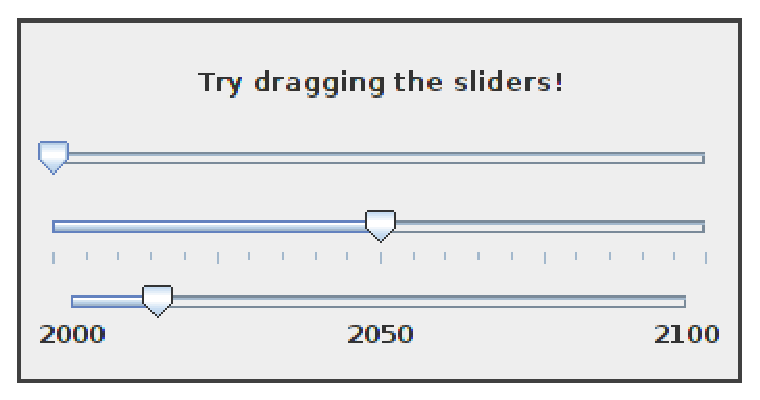
\includegraphics[scale=0.6]{images/slider-demo.eps}
}



\noindent Here, the second slider is decorated with tick marks, and the third one
is decorated with labels. It's possible for a single slider to have both types
of decorations.


The most commonly used constructor for \classname{JSliders} specifies the start
and end of the range of values for the slider and its initial value when it
first appears on the screen:

\displaycode{public JSlider(int minimum, int maximum, int value)}\donedisplaycode


\noindent If the parameters are omitted, the values 0, 100, and 50 are used. By
default, a slider is horizontal, but you can make it vertical by calling its
method \code{setOrientation(JSlider.VERTICAL)}. The current value of a
\classname{JSlider} can be read at any time with its \code{getValue()} method,
which returns a value of type \ptype{int}. If you want to change the
value, you can do so with the method \code{setValue(n)}, which takes a
parameter of type \ptype{int}.


If you want to respond immediately when the user changes the value of a
slider, you can register a listener with the slider. \code{JSliders}, unlike
other components we have seen, do not generate \code{ActionEvents}. Instead,
they generate events of type \classname{ChangeEvent}. 
\classname{ChangeEvent} and
related classes are defined in the package \code{javax.swing.event} rather
than \code{java.awt.event}, so if you want to use \code{ChangeEvents}, you
should \code{import javax.swing.event.*} at the beginning of your program.
You must also define some object to implement the \classname{ChangeListener}
interface, and you must register the change listener with the slider by calling
its \code{addChangeListener()} method. A \classname{ChangeListener} must provide
a definition for the method:

\displaycode{public void stateChanged(ChangeEvent evt)}\donedisplaycode


\noindent This method will be called whenever the value of the slider changes. Note
that it will be called when you change the value with the \code{setValue()}
method, as well as when the user changes the value. In the
\code{stateChanged()} method, you can call \code{evt.getSource()} to find
out which object generated the event. If you want to know whether the user
generated the change event, call the slider's \code{getValueIsAdjusting()}
method, which returns true if the user is dragging the knob on the slider.


Using tick marks on a slider is a two-step process: Specify the interval
between the tick marks, and tell the slider that the tick marks should be
displayed. There are actually two types of tick marks, ``major" tick marks and
``minor" tick marks. You can have one or the other or both. Major tick marks are
a bit longer than minor tick marks. The method \code{setMinorTickSpacing(i)}
indicates that there should be a minor tick mark every \code{i} units along
the slider. The parameter is an integer. (The spacing is in terms of values on
the slider, not pixels.) For the major tick marks, there is a similar command,
\code{setMajorTickSpacing(i)}. Calling these methods is not enough to make
the tick marks appear. You also have to call \code{setPaintTicks(true)}. For
example, the second slider in the above illustration was created and configured using
the commands:

\displaycode{slider2 = new JSlider();  // (Uses default min, max, and value.)
slider2.addChangeListener(this);
slider2.setMajorTickSpacing(25);
slider2.setMinorTickSpacing(5);
slider2.setPaintTicks(true);}\donedisplaycode



Labels on a slider are handled similarly. You have to specify the labels and
tell the slider to paint them. Specifying labels is a tricky business, but the
\classname{JSlider} class has a method to simplify it. You can create a set of labels and
add them to a slider named \code{sldr} with the command:

\displaycode{sldr.setLabelTable( sldr.createStandardLabels(i) );}\donedisplaycode


\noindent where \code{i} is an integer giving the spacing between the labels. To
arrange for the labels to be displayed, call \code{setPaintLabels(true)}. For
example, the third slider in the above illustration was created and configured with
the commands:

\displaycode{slider3 = new JSlider(2000,2100,2014);
slider3.addChangeListener(this);
slider3.setLabelTable( slider3.createStandardLabels(50) );
slider3.setPaintLabels(true);}\donedisplaycode

   

   
   

   



\section{Basic Layout}\label{GUI1.7}



\start{{\Large C}omponents} are the fundamental building blocks
of a graphical user interface.  But you have to do more with components besides create them.
Another aspect of GUI programming is \newword{laying out} components on the screen,
that is, deciding where they are drawn and how big they are. You have probably
noticed that computing coordinates can be a difficult problem, especially if
you don't assume a fixed size for the drawing area. Java has a solution for this, as
well.


Components are the visible objects that make up a GUI. Some components are
\newword{containers}, which can hold other components.  Containers in
Java are objects that belong to some subclass of \code{java.awt.Container}.
The content pane of a  \classname{JFrame}
is an example of a container. The standard class
\classname{JPanel}, which we have mostly used as a drawing surface up until now, is
another example of a container.


Because a \classname{JPanel} object is a
container, it can hold other components.  Because a
\classname{JPanel} is itself a component, you can add a \classname{JPanel} 
to another \classname{JPanel}. This makes complex
nesting of components possible. \classname{JPanels} can be used to organize
complicated user interfaces, as shown in this illustration:


\par\dumpfigure{
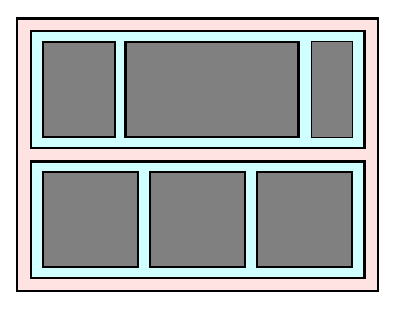
\includegraphics{images/panels-in-layout.eps}
}

  
\noindent In this picture, a large panel holds two smaller panels.  Each of the two smaller
panels in turn holds three components.


The components in a container must be ``laid out," which means setting their
sizes and positions. It's possible to program the layout yourself, but
layout is ordinarily done by a \newword{layout manager}. A
layout manager is an object associated with a container that implements some
policy for laying out the components in that container. Different types of
layout manager implement different policies.  In this section, we will cover
the three most common types of layout manager, and then we will look at
several programming examples that use components and layout.


Every container has a default layout manager and has 
an instance method, \code{setLayout()}, that takes
a parameter of type \classname{LayoutManager} and that is used to specify
a different layout manager for the container.
Components are added to a container by calling
an instance method named \code{add()} in the container object.  There
are actually several versions of the \code{add()} method, with different
parameter lists.  Different versions of \code{add()} are appropriate
for different layout managers, as we will see below.
   
   
\subsection{Basic Layout Managers}\label{GUI1.7.1}



Java has a variety of standard layout managers that
can be used as parameters in the \code{setLayout()} method.  They are defined by
classes in the package \code{java.awt}.  Here, we will look at
just three of these layout manager classes: \classname{FlowLayout},
\classname{BorderLayout}, and \classname{GridLayout}.

   

A \classname{FlowLayout} simply lines up components in a row across the
container.  The size of each component is equal to that component's ``preferred size."
After laying out as many items as will fit in a row
across the container, the layout manager will move on to the next row.
The default layout for a \classname{JPanel} is a
\classname{FlowLayout};  that is, a \classname{JPanel} uses a
\classname{FlowLayout} unless you specify a different layout manager by
calling the panel's \code{setLayout()} method.
   

The components in a given row can be either left-aligned, right-aligned, or centered within
that row, and there can be horizontal and vertical gaps between components. If the default constructor,
``\code{new FlowLayout()}", is used, then the components on each row will be centered
and both the horizontal and the vertical gaps will be five pixels.  The constructor

\displaycode{public FlowLayout(int align, int hgap, int vgap)}\donedisplaycode


\noindent can be used to specify alternative alignment and gaps. The possible values
of \code{align} are \code{FlowLayout.LEFT}, \code{FlowLayout.RIGHT}, and
\code{FlowLayout.CENTER}.
   

Suppose that \code{container} is a container object that is using a \classname{FlowLayout}
as its layout manager.  Then, a component, \code{comp}, can be added to the container with
the statement
  
\displaycode{container.add(comp);}\donedisplaycode

   
\noindent The \classname{FlowLayout} will line up all the components that have been
added to the container in this way.  They will be lined up in the order in which they
were added.  For example, this picture shows five buttons in a panel that uses
a \classname{FlowLayout}:


\par\dumpfigure{
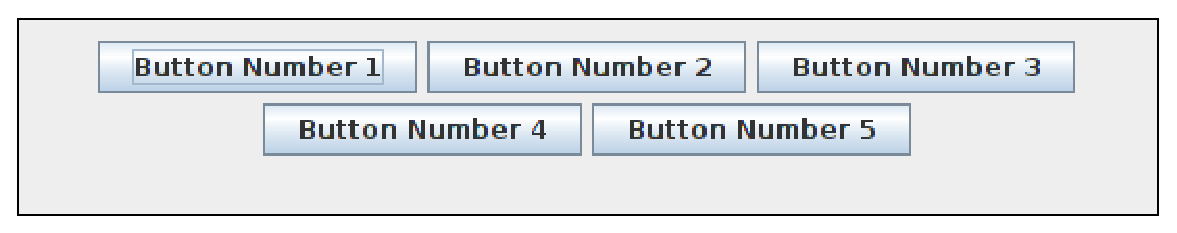
\includegraphics[scale=0.6]{images/flow-layout-demo.eps}
}

   
\noindent Note that since the five buttons will not fit in a single row across the panel,
they are arranged in two rows.  In each row, the buttons are grouped together and are
centered in the row.  The buttons were added to the panel using the statements:
   
\displaycode{panel.add(button1);
panel.add(button2);
panel.add(button3);
panel.add(button4);
panel.add(button5);}\donedisplaycode

   

When a container uses a layout manager, the layout manager is ordinarily responsible
for computing the preferred size of the container (although a different preferred size
could be set by calling the container's \code{setPreferredSize} method).  A
\classname{FlowLayout} prefers to put its components in a single row,
so the preferred width is the total of the preferred widths of all the components, plus
the horizontal gaps between the components.  The preferred height is the maximum
preferred height of all the components.


\mybreak

   

A \classname{BorderLayout} layout manager is designed to display
one large, central component, with up to four smaller components arranged around
the edges of the central component.  If a container, \code{cntr}, is
using a \classname{BorderLayout}, then a component, \code{comp},
should be added to the container using a statement of the form
   
\displaycode{cntr.add( comp, borderLayoutPosition );}\donedisplaycode

   
\noindent where \code{borderLayoutPosition} specifies what position the component
should occupy in the layout and is given as one of the constants
\code{BorderLayout.CENTER}, \code{BorderLayout.NORTH}, 
\code{BorderLayout.SOUTH}, \code{BorderLayout.EAST}, 
or \code{BorderLayout.WEST}.  The meaning of the five
positions is shown in this diagram:
   

\par\dumpfigure{
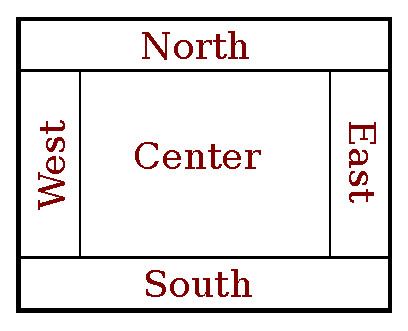
\includegraphics[scale=0.6]{images/border-layout.eps}
}
   

\noindent Note that a border layout can contain fewer than five components,
so that not all five of the possible positions need to be filled.
It would be very unusual, however, to have no center component.
   

A \classname{BorderLayout} sets the sizes of its components
as follows:  The \code{NORTH} and \code{SOUTH} components (if
present) are shown at their preferred heights, but their width is set equal
to the full width of the container.  The \code{EAST} and \code{WEST}
components are shown at their preferred widths, but their height is set
to the height of the container, minus the space occupied by the \code{NORTH}
and \code{SOUTH} components.  Finally, the \code{CENTER} component
takes up any remaining space.  The preferred size of the \code{CENTER}
component is ignored when the layout is done, but it is taken into account when
the preferred size of the container as a whole is computed.  You should make sure that the components
that you put into a \classname{BorderLayout} are suitable for the
positions that they will occupy.  A horizontal slider or text field, for example,
would work well in the \code{NORTH} or \code{SOUTH} position, but
wouldn't make much sense in the \code{EAST} or \code{WEST} position.



The default constructor, \code{new BorderLayout()}, leaves no space
between components.  If you would like to leave some space,
you can specify horizontal and vertical gaps in the constructor of the
\code{BorderLayout} object. For example, if you say

\displaycode{panel.setLayout(new BorderLayout(5,7));}\donedisplaycode


\noindent then the layout manager will insert horizontal gaps of 5 pixels between
components and vertical gaps of 7 pixels between components. The background
color of the container will show through in these gaps.  The default layout for
the original content pane that comes with a \classname{JFrame} 
is a \code{BorderLayout} with no horizontal or vertical gap.
   

\mybreak



Finally, we consider the \classname{GridLayout} layout manager.
A grid layout lays out components in a grid containing rows and columns of equal
sized rectangles. This illustration shows how the components would be arranged
in a grid layout with 4 rows and 3 columns:
   

\par\dumpfigure{
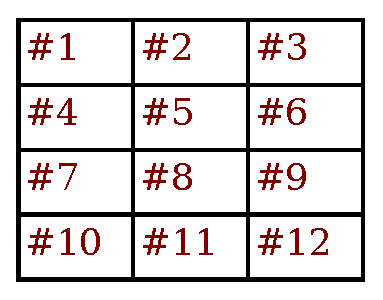
\includegraphics[scale=0.6]{images/grid-layout.eps}
}
   
   
\noindent If a container uses a
\classname{GridLayout}, the appropriate \code{add} method for the container
takes a single parameter of type \classname{Component} (for example: 
\code{cntr.add(comp)}).  Components are added to the grid in the order shown;
that is, each row is filled from left to right before going on the next row.


The constructor for a \classname{GridLayout} takes the form 
``\code{new GridLayout(R,C)}", where \code{R} is the number of rows
and \code{C} is the number of columns. If you want
to leave horizontal gaps of \code{H} pixels between columns and vertical gaps
of \code{V} pixels between rows, use ``\code{new GridLayout(R,C,H,V)}"
instead.


When you use a \classname{GridLayout}, it's probably good form to add just
enough components to fill the grid. However, this is not required. In fact, as
long as you specify a non-zero value for the number of rows, then the number of
columns is essentially ignored. The system will use just as many columns as are
necessary to hold all the components that you add to the container. If you want
to depend on this behavior, you should probably specify zero as the number of
columns. You can also specify the number of rows as zero. In that case, you
must give a non-zero number of columns. The system will use the specified
number of columns, with just as many rows as necessary to hold the components
that are added to the container.


Horizontal grids, with a single row, and vertical grids, with a single
column, are very common. For example, suppose that \code{button1},
\code{button2}, and \code{button3} are buttons and that you'd like to
display them in a horizontal row in a panel. If you use a horizontal grid for
the panel, then the buttons will completely fill that panel and will all be the
same size.  The panel can be created as follows:

\displaycode{JPanel buttonBar = new JPanel();
buttonBar.setLayout( new GridLayout(1,3) );
    // (Note:  The "3" here is pretty much ignored, and
    //  you could also say "new GridLayout(1,0)".
    //  To leave gaps between the buttons, you could use
    //  "new GridLayout(1,0,5,5)".)
buttonBar.add(button1);
buttonBar.add(button2);
buttonBar.add(button3);}\donedisplaycode


\noindent You might find this button bar to be more attractive than the one
that uses the default \classname{FlowLayout} layout manager.





\subsection{Borders}\label{GUI1.7.2}

   

We have seen how to leave gaps between the components in a container, but what
if you would like to leave a border around the outside of the container?  This
problem is not handled by layout managers.  Instead, borders in Swing are represented
by objects.  A \classname{Border} object can be added to any \classname{JComponent},
not just to containers. Borders can be more than just empty space.
The class \code{javax.swing.BorderFactory} contains a
large number of static methods for creating border objects. For example, the
function

\displaycode{BorderFactory.createLineBorder(Color.BLACK)}\donedisplaycode


\noindent returns an object that represents a one-pixel wide black line around the
outside of a component. If \code{comp} is a \code{JComponent}, a border can
be added to \code{comp} using its \code{setBorder()} method. For
example:

\displaycode{comp.setBorder( BorderFactory.createLineBorder(Color.BLACK) );}\donedisplaycode



Once a border has been set for a \code{JComponent}, the border is drawn
automatically, without any further effort on the part of the programmer. The
border is drawn along the edges of the component, just inside its boundary. The
layout manager of a \code{JPanel} or other container will take the space
occupied by the border into account. The components that are added to the
container will be displayed in the area inside the border. I don't recommend
using a border on a \code{JPanel} that is being used as a drawing surface.
However, if you do this, you should take the border into account. If you draw
in the area occupied by the border, that part of your drawing will be covered
by the border.


Here are some of the static methods that can be used to create borders:



\mylist{

\myitem \codedef{BorderFactory.createEmptyBorder(top,left,bottom,right)}
--- leaves an empty border around the edges of a component. Nothing is drawn in
this space, so the background color of the component will appear in the area occupied by the
border. The parameters are integers that give the width of the border along the
top, left, bottom, and right edges of the component. This is actually very
useful when used on a \classname{JPanel} that contains other components. It puts
some space between the components and the edge of the panel.  It can also be
useful on a \classname{JLabel}, which otherwise would not have any
space between the text and the edge of the label.
\myitem \codedef{BorderFactory.createLineBorder(color,thickness)} ---
draws a line around all four edges of a component. The first parameter is of
type \classname{Color} and specifies the color of the line. The second parameter
is an integer that specifies the thickness of the border, in pixels. If the second
parameter is omitted, a line of thickness 1 is drawn.
\myitem \codedef{BorderFactory.createMatteBorder(top,left,bottom,right,color)}
--- is similar to \code{createLineBorder}, except that you can specify
individual thicknesses for the top, left, bottom, and right edges of the
component.
\myitem \codedef{BorderFactory.createEtchedBorder()}
--- creates a border that looks like a groove etched around the boundary of the
component. The effect is achieved using lighter and darker shades of the
component's background color, and it does not work well with every background
color.
\myitem \codedef{BorderFactory.createLoweredBevelBorder()}---gives a
component a three-dimensional effect that makes it look like it is lowered into
the computer screen. As with an EtchedBorder, this only works well for certain
background colors.
\myitem \codedef{BorderFactory.createRaisedBevelBorder()}---similar
to a LoweredBevelBorder, but the component looks like it is raised above the
computer screen.
\myitem \codedef{BorderFactory.createTitledBorder(title)}---creates a
border with a title. The title is a \classname{String}, which is displayed in the
upper left corner of the border.
}



There are many other methods in the \code{BorderFactory} class, most of
them providing variations of the basic border styles given here. The following
illustration shows six components with six different border styles. The text in each
component is the command that created the border for that component:


\par\dumpfigure{
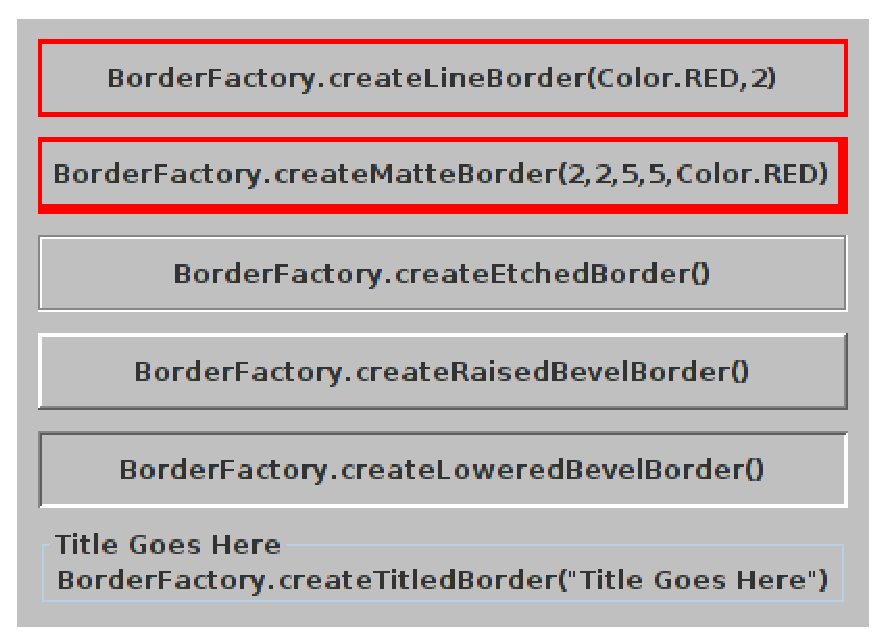
\includegraphics[scale=0.6]{images/border-demo.eps}
}


\noindent (The source code for the program that produced this picture can be found
in \sourceref{BorderDemo.java}.)



   
\subsection{SliderAndButtonDemo}\label{GUI1.7.3}



Now that we have looked at components and layouts, it's time to put
them together into some complete programs.  We start with a simple demo
that uses a \classname{JLabel}, three \classname{JButtons},
and a couple of \classname{JSliders}, all laid out in a
\classname{GridLayout}, as shown in this picture:


\par\dumpfigure{
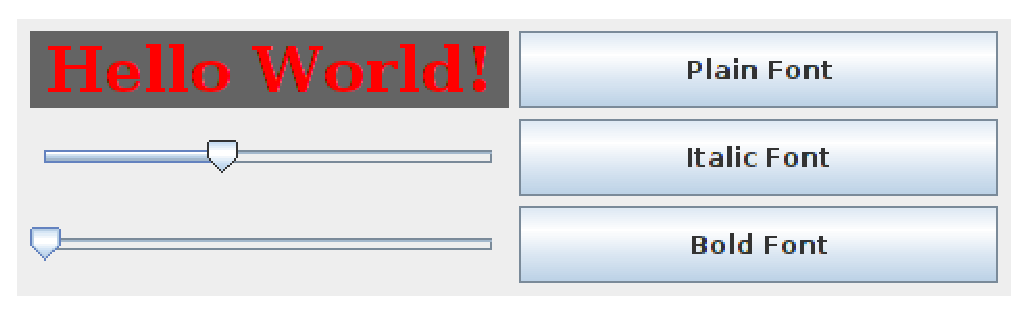
\includegraphics[scale=0.6]{images/slider-and-button-demo.eps}
}


\noindent The sliders in this program control the foreground and background color of the label,
and the buttons control its font style.  Writing this program is a matter of creating
the components, laying them out, and programming listeners to respond to events
from the sliders and buttons.  My program is defined as a subclass of \classname{JPanel}
that implements
\classname{ChangeListener} and \classname{ActionListener}, so that the
panel itself can act as the listener for change events from the sliders and action events from the buttons.
In the constructor, the six components are created and configured,
a \classname{GridLayout} is installed as the layout manager for
the panel, and the components are added to the panel:

   
\displaycode{/* Create the display label, with properties to match the
       values of the sliders and the setting of the combo box. */

displayLabel = new JLabel("Hello World!", JLabel.CENTER);
displayLabel.setOpaque(true);
displayLabel.setBackground( new Color(100,100,100) );
displayLabel.setForeground( Color.RED );
displayLabel.setFont( new Font("Serif", Font.BOLD, 30) );
displayLabel.setBorder(BorderFactory.createEmptyBorder(0,8,0,8));

/* Create the sliders, and set up the panel to listen for
   ChangeEvents that are generated by the sliders. */

bgColorSlider = new JSlider(0,255,100);
bgColorSlider.addChangeListener(this);

fgColorSlider = new JSlider(0,100,0);
fgColorSlider.addChangeListener(this);

/* Create four buttons to control the font style, and set up the
   panel to listen for ActionEvents from the buttons. */

JButton plainButton = new JButton("Plain Font");
plainButton.addActionListener(this);
JButton italicButton = new JButton("Italic Font");
italicButton.addActionListener(this);
JButton boldButton = new JButton("Bold Font");
boldButton.addActionListener(this);


/* Set the layout for the panel, and add the four components. 
       Use a GridLayout with 3 rows and 2 columns, and with
       5 pixels between components. */

setLayout(new GridLayout(3,2,5,5));
add(displayLabel);
add(plainButton);
add(bgColorSlider);
add(italicButton);
add(fgColorSlider);
add(boldButton);}\donedisplaycode

   

The class also defines the methods required by the \classname{ActionListener}
and \classname{ChangeListener} interfaces.  The \code{actionPerformed()}
method is called when the user clicks one of the buttons.  This method changes
the font in the \classname{JLabel}, where the font depends on which button was
clicked.  To determine which button was clicked, the method uses \code{evt.getActionCommand()},
which returns the text from the button:
   
\displaycode{public void actionPerformed(ActionEvent evt) \{
    String cmd = evt.getActionCommand();
    if (cmd.equals("Plain Font")) \{
        displayLabel.setFont( new Font("Serif", Font.PLAIN, 30) );
    \}
    else if (cmd.equals("Italic Font")) \{
        displayLabel.setFont( new Font("Serif", Font.ITALIC, 30) );
    \}
    else if (cmd.equals("Bold Font")) \{
        displayLabel.setFont( new Font("Serif", Font.BOLD, 30) );
    \}
\}}\donedisplaycode

   
\noindent And the \code{stateChanged()} method, which is called when the user
manipulates one of the sliders, uses the value on the slider to compute a new
foreground or background color for the label.  The method checks
\code{evt.getSource()} to determine which slider was changed:
   
\displaycode{public void stateChanged(ChangeEvent evt) \{
    if (evt.getSource() == bgColorSlider) \{
        int bgVal = bgColorSlider.getValue();
        displayLabel.setBackground( new Color(bgVal,bgVal,bgVal) );
            // NOTE:  The background color is a shade of gray,
            //        determined by the setting on the slider.
    \}
    else \{
        float hue = fgColorSlider.getValue()/100.0f;
        displayLabel.setForeground( Color.getHSBColor(hue, 1.0f, 1.0f) );
            // Note:  The foreground color ranges through all the colors
            // of the spectrum.
    \}
\}}\donedisplaycode

   
\noindent Note that the slider variables are global variables in the program because they are referenced
in the \code{stateChanged()} method as well as in the constructor.  On the other hand, the
button variables are local variables in the constructor because that is the only place where they
are used.  The complete source code for this example is in the file 
\sourceref{SliderAndButtonDemo.java}.
   

   

\subsection{A Simple Calculator}\label{GUI1.7.4}



As our next example, we look briefly at an example that uses nested subpanels
to build a more complex user interface.  The program has two \classname{JTextFields}
where the user can enter two numbers, four \classname{JButtons} that the
user can click to add, subtract, multiply, or divide the two numbers, and
a \classname{JLabel} that displays the result of the operation.  Here
is a picture from the program:


\par\dumpfigure{
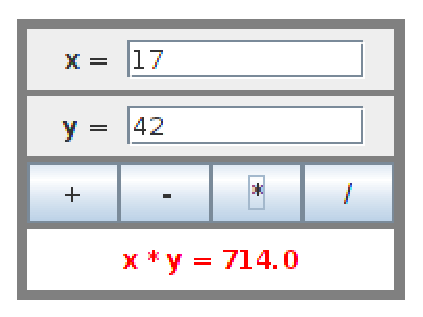
\includegraphics[scale=0.6]{images/simple-calc.eps}
}

 
\noindent This example uses a panel with a
\classname{GridLayout} that has four rows and one column.  In this
case, the layout is created with the statement:
   
\displaycode{setLayout(new GridLayout(4,1,3,3));}\donedisplaycode


\noindent which allows a 3-pixel gap between the rows where the gray background color
of the panel is visible.
   

The first row of the grid layout actually contains two components,
a \classname{JLabel} displaying the text ``\code{x~=}"
and a \classname{JTextField}.  A grid layout can only
have one component in each position.  In this case, the component in the first row
is a \classname{JPanel}, a subpanel that is nested inside
the main panel.  This subpanel in turn contains the label and text
field.  This can be programmed as follows:
   
\displaycode{xInput = new JTextField("0", 10); // Create a text field sized to hold 10 chars.
JPanel xPanel = new JPanel();     // Create the subpanel.
xPanel.add( new JLabel(" x = ")); // Add a label to the subpanel.
xPanel.add(xInput);               // Add the text field to the subpanel

add(xPanel);                      // Add the subpanel to the main panel.}\donedisplaycode


\noindent The subpanel uses the default \classname{FlowLayout} layout manager,
so the label and text field are simply placed next to each other in the
subpanel at their preferred size, and are centered in the subpanel.
   

Similarly, the third row of the grid layout is a subpanel that contains four
buttons.  In this case, the subpanel uses a \classname{GridLayout} with
one row and four columns, so that the buttons are all the same size and completely
fill the subpanel.
   

One other point of interest in this example is the \code{actionPerformed()}
method that responds when the user clicks one of the buttons.  This method must
retrieve the user's numbers from the text field, perform the appropriate 
arithmetic operation on them (depending on which button was clicked), and
set the text of the \classname{JLabel} (named \code{answer}) 
to represent the result.  However, the contents of
the text fields can only be retrieved as strings, and these strings must be
converted into numbers.  If the conversion fails, the label is set to display 
an error message:
   
\displaycode{public void actionPerformed(ActionEvent evt) \{
   
   double x, y;  // The numbers from the input boxes.
   
   try \{
      String xStr = xInput.getText();
      x = Double.parseDouble(xStr);
   \}
   catch (NumberFormatException e) \{
          // The string xStr is not a legal number.
      answer.setText("Illegal data for x.");
      xInput.requestFocusInWindow();
      return;
   \}
   
   try \{
      String yStr = yInput.getText();
      y = Double.parseDouble(yStr);
   \}
   catch (NumberFormatException e) \{
         // The string yStr is not a legal number.
      answer.setText("Illegal data for y.");
      yInput.requestFocusInWindow();
      return;
   \}
   
   /* Perform the operation based on the action command from the
    button.  The action command is the text displayed on the button.
    Note that division by zero produces an error message. */
   
   String op = evt.getActionCommand();
   if (op.equals("+"))
      answer.setText( "x + y = " + (x+y) );
   else if (op.equals("-"))
      answer.setText( "x - y = " + (x-y) );
   else if (op.equals("*"))
      answer.setText( "x * y = " + (x*y) );
   else if (op.equals("/")) \{
      if (y == 0)
         answer.setText("Can't divide by zero!");
      else
         answer.setText( "x / y = " + (x/y) );
   \}
   
\} // end actionPerformed()}\donedisplaycode

   
\noindent The complete source code for this example can be found in \sourceref{SimpleCalc.java}.


   

   
\subsection{Using a null Layout}\label{GUI1.7.5}




As mentioned above, it is possible to do without a layout manager altogether.
For our next example, we'll look at a panel that does not use a layout
manager.  If you set the layout manager of a container to be \code{null}, 
by calling \code{container.setLayout(null)}, then
you assume complete responsibility for positioning and sizing the components in
that container.


If \code{comp} is any component, then the statement

\displaycode{comp.setBounds(x, y, width, height);}\donedisplaycode


\noindent puts the top left corner of the component at the point \code{(x,y)},
measured in the coordinate system of the container that contains the
component, and it sets the width and height of the component to the specified
values. You should only set the bounds of a component if the container that
contains it has a null layout manager. In a container that has a non-null
layout manager, the layout manager is responsible for setting the bounds, and
you should not interfere with its job.


Assuming that you have set the layout manager to \code{null}, you can call
the \code{setBounds()} method any time you like. (You can even make a
component that moves or changes size while the user is watching.) If you are
writing a panel that has a known, fixed size, then you can set the bounds of
each component in the panel's constructor.  Note that you must also add
the components to the panel, using the panel's \code{add(component)}
instance method; otherwise, the component will not appear on the screen.
   

Our example contains four components: two buttons, a label, and a
panel that displays a checkerboard pattern:


\par\dumpfigure{
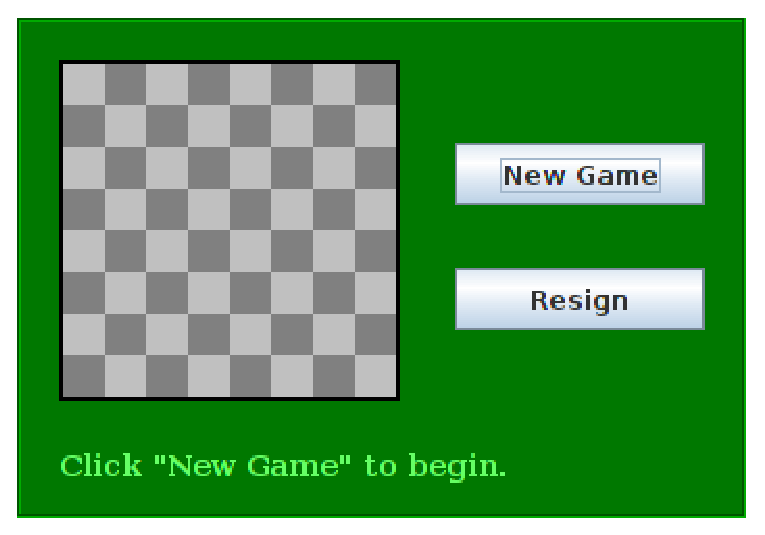
\includegraphics[scale=0.6]{images/null-layout-demo.eps}
}


\noindent This is just an example of using a null layout; it doesn't do anything,
except that clicking the buttons changes the text of the label. (We will use
this example in Section~\ref{arrays.5} as a starting point for a checkers game.)


The panel in this program is defined by the class \classname{NullLayoutDemo},
which is created as a subclass of \classname{JPanel}.  The four
components are created and added to the panel in the constructor.
Then the \code{setBounds()} method of each component is
called to set the size and position of the component:

\displaycode{public NullLayoutDemo() \{

    setLayout(null);  // I will do the layout myself!

    setBackground(new Color(0,120,0));  // A dark green background.

    setBorder( BorderFactory.createEtchedBorder() ); 

    setPreferredSize( new Dimension(350,240) );

    /* Create the components and add them to the content pane.  If you
         don't add them to a container, they won't appear, even if
         you set their bounds! */

    board = new Checkerboard();
        // (Checkerboard is a subclass of JPanel, defined below as a static
        //  nested class inside the main class.)
    add(board);

    newGameButton = new JButton("New Game");
    newGameButton.addActionListener(this);
    add(newGameButton);

    resignButton = new JButton("Resign");
    resignButton.addActionListener(this);
    add(resignButton);

    message = new JLabel("Click \1"New Game\1" to begin.");
    message.setForeground( new Color(100,255,100) ); // Light green.
    message.setFont(new Font("Serif", Font.BOLD, 14));
    add(message);

    /* Set the position and size of each component by calling
         its setBounds() method. */

    board.setBounds(20,20,164,164);
    newGameButton.setBounds(210, 60, 120, 30);
    resignButton.setBounds(210, 120, 120, 30);
    message.setBounds(20, 200, 330, 30);

\} // end constructor}\donedisplaycode



It's fairly easy in this case to get a reasonable layout. It's much
more difficult to do your own layout if you want to allow for changes of size.
In that case, you have to respond to changes in the container's size by
recomputing the sizes and positions of all the components that it contains. If
you want to respond to changes in a container's size, you can register an
appropriate listener with the container. Any component generates an event of
type \classname{ComponentEvent} when its size changes (and also when it is moved,
hidden, or shown). You can register a \classname{ComponentListener} with the
container and respond to resize events by recomputing the sizes and
positions of all the components in the container. Consult a Java reference for
more information about \classname{ComponentEvents}. However, my real advice is
that if you want to allow for changes in the container's size, try to find a
layout manager to do the work for you.


The complete source code for this example is in \sourceref{NullLayoutDemo.java}.




\subsection{A Little Card Game}\label{GUI1.7.6}

   


For a final example, let's look at something a little more interesting as a program.
The example is a simple card game in which you look at a playing card and try to
predict whether the next card will be higher or lower in value. (Aces have the
lowest value in this game.) You've seen a text-oriented version of the same
game in Subsection~\ref{OOP.4.3}. Section~\ref{OOP.4} also introduced
\classname{Deck}, \classname{Hand}, and \classname{Card} 
classes that are used by the program. In this GUI version of the game, 
you click on a button to make your
prediction. If you predict wrong, you lose. If you make three correct
predictions, you win. After completing one game, you can click the ``New Game"
button to start a new game. Here is
what the program looks like in the middle of a game:


\par\dumpfigure{
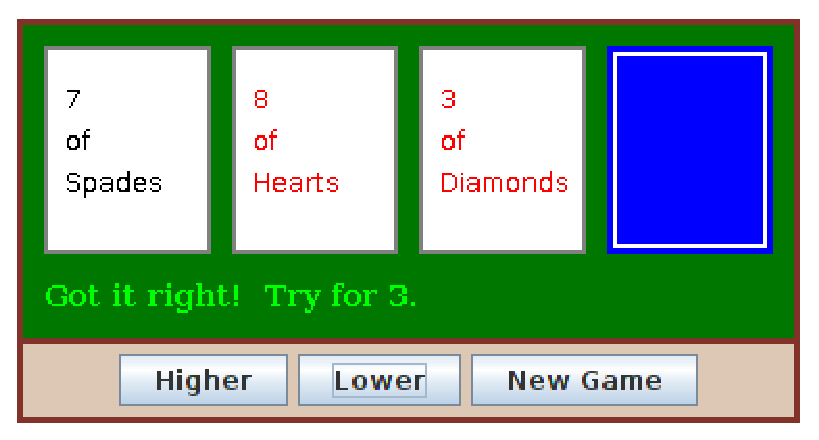
\includegraphics[scale=0.6]{images/high-low-gui.eps}
}



\noindent The complete source code for the panel can be found in the file
\sourceref{HighLowGUI.java}.  I encourage you to compile and run it.
Remember that you also need \sourceref{Card.java}, \sourceref{Deck.java}, 
and \sourceref{Hand.java}, since they define classes that are used in the program.
   

The overall structure of the main panel in this example should be reasonably clear:
It has three buttons in a subpanel at the bottom of the main panel and a large drawing
surface that displays the cards and a message.  (The cards and message are not
components in this example; they are drawn using the graphics context in the panel's
\code{paintComponent()} method.)  The main panel uses a
\classname{BorderLayout}.  The drawing surface occupies the
\code{CENTER} position of the border layout.  The subpanel that contains
the buttons occupies the \code{SOUTH} position of the border layout,
and the other three positions of the borderlayout are empty.
   

The drawing surface is defined by a nested class named \classname{CardPanel},
which is subclass of \classname{JPanel}.  I have chosen to let the
drawing surface object do most of the work of the game: It listens for
events from the three buttons and responds by taking the appropriate actions.
The main panel is defined by \classname{HighLowGUI} itself, which
is also a subclass of \classname{JPanel}.  The constructor
of the \classname{HighLowGUI} class creates all the other
components, sets up event handling, and lays out the components:

\displaycode{public HighLowGUI() \{   // The constructor.
            
   setBackground( new Color(130,50,40) );
   
   setLayout( new BorderLayout(3,3) );  // BorderLayout with 3-pixel gaps.
   
   CardPanel board = new CardPanel();  // Where the cards are drawn.
   add(board, BorderLayout.CENTER);
   
   JPanel buttonPanel = new JPanel();  // The subpanel that holds the buttons.
   buttonPanel.setBackground( new Color(220,200,180) );
   add(buttonPanel, BorderLayout.SOUTH);
   
   JButton higher = new JButton( "Higher" );
   higher.addActionListener(board);   // The CardPanel listens for events.
   buttonPanel.add(higher);
   
   JButton lower = new JButton( "Lower" );
   lower.addActionListener(board);
   buttonPanel.add(lower);
   
   JButton newGame = new JButton( "New Game" );
   newGame.addActionListener(board);
   buttonPanel.add(newGame);
   
   setBorder(BorderFactory.createLineBorder( new Color(130,50,40), 3) );
   
\}  // end constructor}\donedisplaycode

   
   

The programming of the drawing surface class, \classname{CardPanel},
is a nice example of thinking in terms of a state machine.  (See Subsection~\ref{GUI1.5.4}.)
It is important to think in terms of the states that the game can be in, how the
state can change, and how the response to events can depend on the state. The
approach that produced the original, text-oriented game in 
Subsection~\ref{OOP.4.3} is not appropriate here. Trying to think about
the game in terms of a process that goes step-by-step from beginning to end is
more likely to confuse you than to help you.


The state of the game includes the cards and the message. The cards are
stored in an object of type \classname{Hand}. 
The message is a \classname{String}.
These values are stored in instance variables. There is also another, less
obvious aspect of the state: Sometimes a game is in progress, and the user is
supposed to make a prediction about the next card. Sometimes we are between
games, and the user is supposed to click the ``New Game" button. It's a good
idea to keep track of this basic difference in state. The \classname{CardPanel} class uses a
boolean instance variable named \code{gameInProgress} for this purpose.


The state of the game can change whenever the user clicks on a button. The
\classname{CardPanel} class implements the \classname{ActionListener} interface
and defines an \code{actionPerformed()} method to respond to the user's
clicks. This method simply calls one of three other methods,
\code{doHigher()}, \code{doLower()}, or \code{newGame()}, depending on
which button was pressed. It's in these three event-handling methods that the
action of the game takes place.


We don't want to let the user start a new game if a game is currently in
progress. That would be cheating. So, the response in the \code{newGame()}
method is different depending on whether the state variable
\code{gameInProgress} is true or false. If a game is in progress, the
\code{message} instance variable should be set to be an error message. If a
game is not in progress, then all the state variables should be set to
appropriate values for the beginning of a new game. In any case, the board must
be repainted so that the user can see that the state has changed. The complete
\code{newGame()} method is as follows:

\displaycode{/**
 * Called by the CardPanel constructor, and called by actionPerformed() if
 * the user clicks the "New Game" button.  Start a new game.
 */
void doNewGame() \{
   if (gameInProgress) \{
         // If the current game is not over, it is an error to try
         // to start a new game.
      message = "You still have to finish this game!";
      repaint();
      return;
   \}
   deck = new Deck();   // Create the deck and hand to use for this game.
   hand = new Hand();
   deck.shuffle();
   hand.addCard( deck.dealCard() );  // Deal the first card into the hand.
   message = "Is the next card higher or lower?";
   gameInProgress = true;
   repaint();
\} // end doNewGame()}\donedisplaycode



The \code{doHigher()} and \code{doLower()} methods are almost identical
to each other (and could probably have been combined into one method with a
parameter, if I were more clever). Let's look at the \code{doHigher()}
routine. This is called when the user clicks the ``Higher" button. This only
makes sense if a game is in progress, so the first thing \code{doHigher()}
should do is check the value of the state variable \code{gameInProgress}. If
the value is \code{false}, then \code{doHigher()} should just set up an
error message. If a game is in progress, a new card should be added to the hand
and the user's prediction should be tested. The user might win or lose at this
time. If so, the value of the state variable \code{gameInProgress} must be
set to \code{false} because the game is over. In any case, the board is
repainted to show the new state. Here is the \code{doHigher()} method:

\displaycode{/**
 * Called by actionPerformed() when user clicks the "Higher" button.
 * Check the user's prediction.  Game ends if user guessed
 * wrong or if the user has made three correct predictions.
 */
void doHigher() \{
   if (gameInProgress == false) \{
         // If the game has ended, it was an error to click "Higher",
         // So set up an error message and abort processing.
      message = "Click \1"New Game\1" to start a new game!";
      repaint();
      return;
   \}
   hand.addCard( deck.dealCard() );     // Deal a card to the hand.
   int cardCt = hand.getCardCount();
   Card thisCard = hand.getCard( cardCt - 1 );  // Card just dealt.
   Card prevCard = hand.getCard( cardCt - 2 );  // The previous card.
   if ( thisCard.getValue() \< prevCard.getValue() ) \{
      gameInProgress = false;
      message = "Too bad! You lose.";
   \}
   else if ( thisCard.getValue() == prevCard.getValue() ) \{
      gameInProgress = false;
      message = "Too bad!  You lose on ties.";
   \}
   else if ( cardCt == 4) \{  // The hand is full, after three correct guesses.
      gameInProgress = false;
      message = "You win!  You made three correct guesses.";
   \}
   else \{
      message = "Got it right!  Try for " + cardCt + ".";
   \}
   repaint();
\} // end doHigher()}\donedisplaycode



The \code{paintComponent()} method of the \classname{CardPanel} class
uses the values in the state variables to decide what to show. It displays the
string stored in the \code{message} variable. It draws each of the cards in
the \code{hand}. There is one little tricky bit: If a game is in progress, it
draws an extra face-down card, which is not in the hand, to represent the next
card in the deck. Drawing the cards requires some care and computation. I wrote
a method, ``\code{void drawCard(Graphics g, Card card, int x, int y)}", which
draws a card with its upper left corner at the point \code{(x,y)}. The
\code{paintComponent()} routine decides where to draw each card and calls
this routine to do the drawing. You can check out all the details in the source
code, \sourceref{HighLowGUI.java}.  (The playing cards used in this program
are not very impressive.  A version of the program with images that
actually look like cards can be found in Subsection~\ref{GUI2.1.3}.)

   


   

   
  

   



\section{Menus and Dialogs}\label{GUI1.8}



\start{{\Large W}e have already encountered} many of the basic
aspects of GUI programming, but professional programs use many
additional features.  We will cover some of the advanced features
of Java GUI programming in Chapter~\ref{GUI2}, but in this
section we look briefly at a few more features that are
essential for writing GUI programs.  I will discuss these features
in the context of a
``MosaicDraw" program that is shown in this picture:
   

\par\dumpfigure{
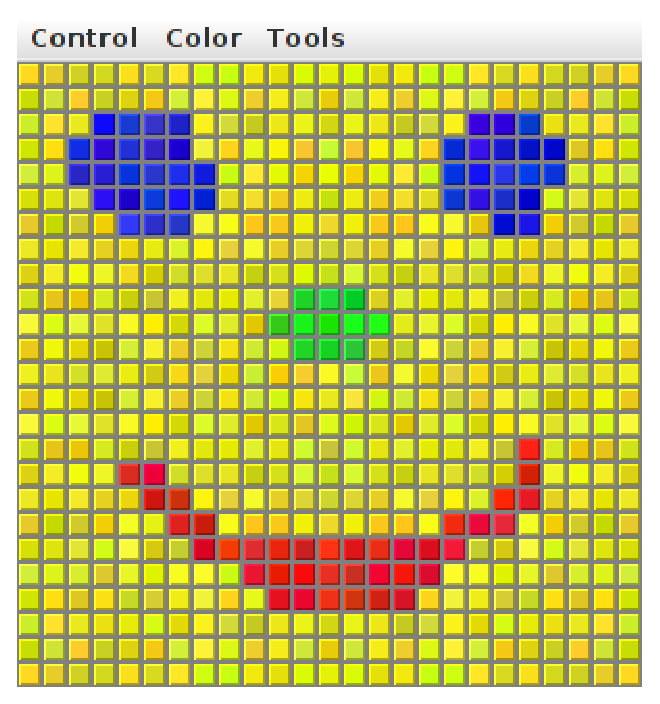
\includegraphics[scale=0.6]{images/mosaic-draw.eps}
}

   
\noindent The source code for the program is in the file \sourceref{MosaicDraw.java}.
The program also requires \sourceref{MosaicPanel.java} and 
\sourceref{MosaicDrawController.java}.  You will want to try it out!


As the user clicks-and-drags the
mouse in the large drawing area of this program, it leaves a trail of little colored
squares. There is some random variation in the color of the squares.  (This is meant
to make the picture look a little more like a real mosaic, which is a picture made out of 
small colored stones in which there would be some natural color variation.)
There is a menu bar above the drawing area.  The ``Control" menu contains
commands for filling and clearing the drawing area, along with a few options that affect
the appearance of the picture.  The ``Color" menu lets the user select the color that will
be used when the user draws.  The ``Tools" menu affects the behavior of the mouse.
Using the default ``Draw" tool, the mouse leaves a trail of single squares.  Using the
``Draw~3x3" tool, the mouse leaves a swath of colored squares that is three squares wide.
There are also ``Erase" tools, which let the user set squares back to their default
black color.
   

The drawing area of the program is a panel that belongs to the \classname{MosaicPanel}
class, a subclass of \classname{JPanel} that is defined in \sourceref{MosaicPanel.java}.
\classname{MosaicPanel} is a highly reusable class for representing mosaics of colored
rectangles.  It was also used behind the scenes in the sample program in Subsection~\ref{subroutines.6.3}.
The \classname{MosaicPanel} class
does not directly support drawing on the mosaic, but it does support setting
the color of each individual square.  The MosaicDraw program installs a mouse listener on
the panel; the mouse listener responds to mousePressed and mouseDragged events on the
panel by setting the color of the square that contains the mouse.  This is a nice example of
applying a listener to an object to do something that was not programmed into the object
itself.


The file  \sourceref{MosaicDraw.java} is a simple class that contains only the \code{main()}
routine for the program.
Most of the programming for MosaicDraw can be found in \sourceref{MosaicDrawController.java}.
(It might have gone into the \classname{MosaicPanel} class, if I had not decided to
use that pre-existing class in unmodified form.)  It is the \classname{MosaicDrawController}
class that creates a \classname{MosaicPanel} object and adds a mouse listener to
it.  It also creates the menu bar that is shown at the top of the program, and it implements all
the commands in the menu bar.  It has an instance method \code{getMosaicPanel()} that
returns a reference to the mosaic panel that it has created, and it has another instance
method \code{getMenuBar()} that returns a menu bar for the program.  These methods are
used to obtain the panel and menu bar so that they can be added to the program's window.
   

I urge you to study MosaicDrawController.java and MosaicDraw.java.  I will not be discussing all aspects
of the code here, but you should be able to understand it all after reading this section. As for
MosaicPanel.java, it uses some techniques that you would not understand at this
point, but I encourage you to at least read the comments in this file to learn about the API
for mosaic panels.
   
\subsection{Menus and Menubars}\label{GUI1.8.1}

   

MosaicDraw is the first example that we have seen that uses a menu bar.  Fortunately,
menus are very easy to use in Java.  The items in a menu are represented by the
class \classname{JMenuItem} (this class and other menu-related classes are
in package \code{javax.swing}).  Menu items are used in almost exactly the
same way as buttons.  In fact, \classname{JMenuItem} and \classname{JButton}
are both subclasses of a class, \classname{AbstractButton}, that defines their
common behavior. In particular, a \classname{JMenuItem} is created using
a constructor that specifies the text of the menu item, such as:
   
\displaycode{JMenuItem fillCommand = new JMenuItem("Fill");}\donedisplaycode

   
\noindent You can add an \classname{ActionListener} to a \classname{JMenuItem}
by calling the menu item's \code{addActionListener()} method.  
The \code{actionPerformed()} method of the
action listener is called when the user selects the item from the menu.  
You can change the text of the item by calling its \code{setText(String)} method,
and you can enable it and disable it using the \code{setEnabled(boolean)} method.
All this works in exactly the same way as for a \classname{JButton}.
   

The main difference between a menu item and a button, of course, is that a menu
item is meant to appear in a menu rather than in a panel.  A menu in Java is
represented by the class \classname{JMenu}.  A \classname{JMenu} has a name,
which is specified in the constructor, and it has an \code{add(JMenuItem)} method that
can be used to add a \classname{JMenuItem} to the menu. For example, the ``Tools"
menu in the MosaicDraw program could be created as follows, where \code{listener}
is a variable of type \code{ActionListener}:

\displaycode{JMenu toolsMenu = new JMenu("Tools");  // Create a menu with name "Tools"

JMenuItem drawCommand = new JMenuItem("Draw");   // Create a menu item.
drawCommand.addActionListener(listener);         // Add listener to menu item.
toolsMenu.add(drawCommand);                      // Add menu item to menu.

JMenuItem eraseCommand = new JMenuItem("Erase"); // Create a menu item.
eraseCommand.addActionListener(listener);        // Add listener to menu item.
toolsMenu.add(eraseCommand);                     // Add menu item to menu.
   .
   .  // Create and add other menu items.
   .}\donedisplaycode

   
\noindent Once a menu has been created, it must be added to a menu bar.  A menu bar is represented
by the class \classname{JMenuBar}.  A menu bar is just a container for menus.
It does not have a name, and its constructor does not have any parameters. It has an
\code{add(JMenu)} method that can be used to add menus to the menu bar.  The name of
the menu then appears in the menu bar.  For example,
the MosaicDraw program uses three menus, \code{controlMenu}, \code{colorMenu},
and \code{toolsMenu}.  We could create a menu bar and add the menus to it with
the statements:
   
\displaycode{JMenuBar menuBar = new JMenuBar();
menuBar.add(controlMenu);
menuBar.add(colorMenu);
menuBar.add(toolsMenu);}\donedisplaycode



The final step in using menus is to use the menu bar in a window such as a \classname{JFrame}.  
We have already seen that a frame has a
``content pane."  The menu bar is another component of the frame, 
not contained inside the content pane.  The \classname{JFrame} class has
an instance method \code{setMenuBar(JMenuBar)} that can be used to set the menu bar.
(There can only be one, so this is a ``set" method rather than an ``add" method.)
In the MosaicDraw program, the menu bar is created by a \classname{MosaicDrawController}
object and can be obtained by calling that object's \code{getMenuBar()} method.
The \code{main()} routine in MosaicDraw.java gets the menu bar from the controller and
adds it to the window.
Here is the basic code that is used (in somewhat modified form) to set up the interface:

\displaycode{MosaicDrawController controller = new MosaicDrawController();

MosaicPanel content = controller.getMosaicPanel();
window.setContentPane( content );  // Use panel from controller as content pane.
   
JMenuBar menuBar = controller.getMenuBar();
window.setJMenuBar( menuBar );    // Use the menu bar from the controller.}\donedisplaycode

     

Using menus always follows the same general pattern:  Create a menu bar.  Create menus
and add them to the menu bar.  Create menu items and add them to the menus (and set up
listening to handle action events from the menu items).  Use the menu bar in a
window by calling the window's \code{setJMenuBar()} method.
   

\mybreak

   

There are other kinds of menu items, defined by subclasses of \classname{JMenuItem},
that can be added to menus.  One of these is \classname{JCheckBoxMenuItem},
which represents menu items that can be in one of two states, selected or not selected.
A \classname{JCheckBoxMenuItem} has the same functionality and is used in
the same way as a \classname{JCheckBox} (see Subsection~\ref{GUI1.6.3}).
Three \classname{JCheckBoxMenuItems} are used in the ``Control" menu
of the MosaicDraw program.  One is used to turn the random color variation of
the squares on and off.  Another turns a symmetry feature on and off; when symmetry is
turned on, the user's drawing is reflected horizontally and vertically to produce
a symmetric pattern.  And the third checkbox menu item shows and hides the
``grouting" in the mosaic; the grouting is the gray lines that are drawn around each
of the little squares in the mosaic.  The menu item that corresponds to the
``Use Randomness" option in the ``Control" menu could be set up with the statements:
       
\displaycode{JMenuItem useRandomnessToggle = new JCheckBoxMenuItem("Use Randomness");
useRandomnessToggle.addActionListener(listener);  // Set up a listener.
useRandomnessToggle.setSelected(true);  // Randomness is initially turned on.
controlMenu.add(useRandomnessToggle);   // Add the menu item to the menu.}\donedisplaycode

   

In my program, the ``Use Randomness" \classname{JCheckBoxMenuItem}
corresponds to a boolean-valued instance variable named \code{useRandomness}
in the \classname{MosaicDrawController} class.
This variable is part of the state of the controller object.
Its value is tested whenever the user draws one
of the squares, to decide whether or not to add a random variation to the color of
the square.  When the user selects the ``Use Randomness" command
from the menu, the state of the \classname{JCheckBoxMenuItem} is reversed,
from selected to not-selected or from not-selected to selected.  The \classname{ActionListener}
for the menu item checks whether the menu item is selected or not, and it changes the
value of \code{useRandomness} to match.  Note that selecting the menu command
does not have any immediate effect on the picture that is shown in the window.  It just
changes the state of the program so that future drawing operations on the part of
the user will have a different effect.  The ``Use Symmetry" option in the ``Control"
menu works in much the same way.  The ``Show Grouting" option is a little different.
Selecting the ``Show Grouting" option does have an immediate effect: The picture is
redrawn with or without the grouting, depending on the state of the menu item.
   

My program uses a single \classname{ActionListener} to respond to
all of the menu items in all the menus.  This is not a particularly good design, but it
is easy to implement for a small program like this one.  The \code{actionPerformed()} method
of the listener object uses the statement

\displaycode{String command = evt.getActionCommand();}\donedisplaycode

   
\noindent to get the action command of the source of the event; this will be the text of
the menu item.  The listener tests the value of \code{command} to determine
which menu item was selected by the user.  If the menu item is a
\classname{JCheckBoxMenuItem}, the listener must check the state of
the menu item.  The menu item is the source of the event that is being processed.
The listener can get its hands on the menu item object by
calling \code{evt.getSource()}.  Since the return value of \code{getSource()}
is of type \classname{Object}, the return value must be type-cast to
the correct type.  Here, for example, is the code that handles the ``Use Randomness"
command:
      
\displaycode{if (command.equals("Use Randomness")) \{
        // Set the value of useRandomness depending on the menu item's state.
   JCheckBoxMenuItem toggle = (JCheckBoxMenuItem)evt.getSource();
   useRandomness = toggle.isSelected();
\}}\donedisplaycode


\noindent (The \code{actionPerformed()} method uses a rather long \code{if..then..else}
statement to check all the possible action commands.  It might be more natural and efficient
use a \code{switch} statement with \code{command} as the selector and
all the possible action commands as cases.)
   

\mybreak



In addition to menu items, a menu can contain lines that separate the menu items
into groups.  In the MosaicDraw program, the ``Control" menu contains such a separator.
A \classname{JMenu} has an instance method \code{addSeparator()}
that can be used to add a separator to the menu.  For example, the separator in the
``Control" menu was created with the statement:
   
\displaycode{controlMenu.addSeparator();}\donedisplaycode

   

A menu can also contain a submenu.  The name of the submenu appears as an item
in the main menu.  When the user moves the mouse over the submenu name, the submenu
pops up.  (There is no example of this in the MosaicDraw program.)  It is very easy
to do this in Java:  You can add one \classname{JMenu} to another
\classname{JMenu} using a statement such as
\code{mainMenu.add(submenu)}, and it becomes a submenu.



\subsection{Dialogs}\label{GUI1.8.2}

 

One of the commands in the ``Color" menu of the MosaicDraw program is
``Custom Color\dots".  When the user selects this command, a new window
appears where the user can select a color.  This window is an example
of a \newword{dialog} or \newword{dialog box}.
A dialog is a type of window that is generally
used for short, single purpose interactions with the user. For example, a
dialog box can be used to display a message to the user, to ask the user a
question, to let the user select a file to be opened,
or to let the user select a color. In Swing, a dialog box is
represented by an object belonging to the class \classname{JDialog}
or to a subclass.


The \classname{JDialog} class is very similar to \classname{JFrame}
and is used in much the same way.
Like a frame, a dialog box is a separate window. Unlike a frame, however, a
dialog is not completely independent. Every dialog is associated with a
frame (or another dialog), which is called its \newword{parent window}. 
The dialog box is dependent on its parent. For
example, if the parent is closed, the dialog box will also be closed. It is
possible to create a dialog box without specifying a parent, but in that case
an invisible frame is created by the system to serve as the parent.


Dialog boxes can be either \newword{modal} or
\newword{modeless}. When a modal dialog is created, its
parent frame is blocked. That is, the user will not be able to interact with
the parent until the dialog box is closed. Modeless dialog boxes do not block
their parents in the same way, so they seem a lot more like independent
windows. In practice, modal dialog boxes are easier to use and are much more
common than modeless dialogs. All the examples we will look at are modal.


Aside from having a parent, a \classname{JDialog} can be created and used in
the same way as a \classname{JFrame}. However, I will not give any examples here of using
\classname{JDialog} directly. Swing has many convenient methods for creating 
common types of dialog boxes. For example, the color choice dialog that appears
when the user selects the ``Custom Color" command in the MosaicDraw program belongs
to the class \classname{JColorChooser}, which is a subclass of
\classname{JDialog}.  The \classname{JColorChooser} class has
a static method that makes color choice dialogs very easy to use:

\displaycode{Color JColorChooser.showDialog(Component parentComp, 
                                        String title, Color initialColor)}\donedisplaycode


\noindent When you call this method, a dialog box appears that allows the user to
select a color. The first parameter specifies the parent of the dialog; the parent
window of the dialog will be the window (if any) that contains \code{parentComp};
this parameter can be \code{null} and it can itself be a frame or dialog object.
The second parameter is a string that appears in the title bar of the dialog box.
And the third parameter, \code{initialColor}, specifies the color that is
selected when the color choice dialog first appears.
The dialog has a sophisticated interface that allows the user to
select a color. When the user presses an ``OK" button, the dialog box
closes and the selected color is returned as the value of the method. The user
can also click a ``Cancel" button or close the dialog box in some other way; in
that case, \code{null} is returned as the value of the method. This is a modal
dialog, and \code{showDialog()} does not return until the user dismisses
the dialog box in some way.  By using this
predefined color chooser dialog, you can write one line of code that will let
the user select an arbitrary color.  Swing also has a \classname{JFileChooser}
class that makes it almost as easy to show a dialog box that lets the user select
a file to be opened or saved.


\mybreak



The \classname{JOptionPane} class includes a variety of methods for
making simple dialog boxes that are variations on three basic types: a
``message" dialog, a ``confirm" dialog, and an ``input" dialog. (The variations
allow you to provide a title for the dialog box, to specify the icon that
appears in the dialog, and to add other components to the dialog box. I will
only cover the most basic forms here.)



A message dialog simply displays a message string to the user. The user
(hopefully) reads the message and dismisses the dialog by clicking the ``OK"
button. A message dialog can be shown by calling the static method:

\displaycode{void JOptionPane.showMessageDialog(Component parentComp, String message)}\donedisplaycode


\noindent The message can be more than one
line long. Lines in the message should be separated by newline characters, \code{\1n}.
New lines will not be inserted automatically, even if the message is very
long.  For example, assuming that the special variable \code{this}
refers to a \classname{Component}:

\displaycode{JOptionPane.showMessageDialog( this, "This program is about to crash!\1n"
                                      + "Sorry about that.");}\donedisplaycode



An input dialog displays a question or request and lets the user type in a
string as a response. You can show an input dialog by calling:

\displaycode{String JOptionPane.showInputDialog(Component parentComp, String question)}\donedisplaycode


\noindent Again, \code{parentComp} can be \code{null}, and
the question can include newline
characters. The dialog box will contain an input box, an ``OK" button, and a
``Cancel" button. If the user clicks ``Cancel", or closes the dialog box in some
other way, then the return value of the method is \code{null}. If the user
clicks ``OK", then the return value is the string that was entered by the user.
Note that the return value can be an empty string (which is not the same as a
\code{null} value), if the user clicks ``OK" without typing anything in the
input box. If you want to use an input dialog to get a numerical value from the
user, you will have to convert the return value into a number (see Subsection~\ref{control.7.2}).
As an example,

\displaycode{String name;
name = JOptionPanel.showInputDialog(null, "Hi!  What's your name?");
if (name == null)
   JOptionPane.showMessageDialog(null, "Well, I'll call you Grumpy.");
else
   JOptionPane.showMessageDialog(null, "Pleased to meet you, " + name);}\donedisplaycode



Finally, a confirm dialog presents a question and three response buttons:
``Yes", ``No", and ``Cancel". A confirm dialog can be shown by calling:

\displaycode{int JOptionPane.showConfirmDialog(Component parentComp, String question)}\donedisplaycode


\noindent The return value tells you the user's response. It is one of the following
constants:



\mylist{

\myitem \code{JOptionPane.YES\_OPTION} --- the user clicked the ``Yes" button
\myitem \code{JOptionPane.NO\_OPTION} --- the user clicked the ``No" button
\myitem \code{JOptionPane.CANCEL\_OPTION} --- the user clicked the ``Cancel" button
\myitem \code{JOptionPane.CLOSE\_OPTION} --- the dialog was closed in some other way.
}



By the way, it is possible to omit the Cancel button from a confirm dialog
by calling one of the other methods in the \code{JOptionPane} class. Just
call:

\displaycode{JOptionPane.showConfirmDialog(
                parent, question, title, JOptionPane.YES\_NO\_OPTION )}\donedisplaycode


\noindent The final parameter is a constant which specifies that only a ``Yes" button
and a ``No" button should be used. The third parameter is a string that will be
displayed as the title of the dialog box window.



A small demo program,
\sourceref{SimpleDialogDemo.java} is available to demonstrate
JColorChooser and several JOptionPane dialogs.

 

   
\subsection{Fine Points of Frames}\label{GUI1.8.3}

   

In previous sections, whenever I used a frame, I created a \classname{JFrame}
object in a \code{main()} routine and installed a panel as the content pane of
that frame.  This works fine, but a more object-oriented approach is to define a subclass
of \classname{JFrame} and to set up the contents of the frame in the constructor
of that class.  This is what I did in the case of the
MosaicDraw program.  \classname{MosaicDraw} is defined as a subclass of
\classname{JFrame}.  The definition of this class is very short, but it illustrates
several new features of frames that I want to discuss:
   
\displaycode{public class MosaicDraw extends JFrame \{
   
   public static void main(String[] args) \{
      JFrame window = new MosaicDraw();
      window.setDefaultCloseOperation(JFrame.EXIT\_ON\_CLOSE);
      window.setVisible(true);
   \}
   
   public MosaicDraw() \{
      super("Mosaic Draw");
      MosaicDrawController controller = new MosaicDrawController();
      setContentPane( controller.getMosaicPanel() );
      setJMenuBar( controller.getMenuBar() );
      pack();
      Dimension screensize = Toolkit.getDefaultToolkit().getScreenSize();
      setLocation( (screensize.width - getWidth())/2, 
                                 (screensize.height - getHeight())/2 );
   \}
   
\}}\donedisplaycode

   

The constructor in this class begins with the statement \code{super("Mosaic Draw")},
which calls the constructor in the superclass, \classname{JFrame}.  The parameter
specifies a title that will appear in the title bar of the window.  The next three lines
of the constructor set up the contents of the window; a \classname{MosaicDrawController}
is created, and the content pane and menu bar of the window are obtained from the
controller.  The next line is something new.  If \code{window} is a variable of
type \classname{JFrame} (or \classname{JDialog}), then the
statement \code{window.pack()} will resize the window so that its size matches
the preferred size of its contents.  (In this case, of course, ``\code{pack()}"
is equivalent to ``\code{this.pack()}"; that is, it refers to the window that is
being created by the constructor.)  The \code{pack()} method is usually the best
way to set the size of a window.  Note that it will only work correctly if every
component in the window has a correct preferred size.  This is only a problem in
two cases:  when a panel is used as a drawing surface and when a panel is used as
a container with a \code{null} layout manager.  In both these cases there is no
way for the system to determine the correct preferred size automatically, and you should
set a preferred size by hand.  For example:
   
\displaycode{panel.setPreferredSize( new Dimension(400, 250) );}\donedisplaycode

   

The last two lines in the constructor position the window so that it is exactly
centered on the screen. The line
   
\displaycode{Dimension screensize = Toolkit.getDefaultToolkit().getScreenSize();}\donedisplaycode

   
\noindent determines the size of the screen.  The size of the screen is \code{screensize.width}
pixels in the horizontal direction and \code{screensize.height} pixels in the vertical
direction. The \code{setLocation()} method of the frame sets the position of the
upper left corner of the frame on the screen.  The expression ``\code{screensize.width~-~getWidth()}"
is the amount of horizontal space left on the screen after subtracting the width of the window.
This is divided by 2 so that half of the empty space will be to the left of the window, leaving
the other half of the space to the right of the window.
Similarly, half of the extra vertical space is above the window, and half is below.


Note that the constructor has created the window and set its size and position, but that
at the end of the constructor, the window is not yet visible on the screen.  (More exactly,
the constructor has created the window \textit{object}, but the visual representation of
that object on the screen has not yet been created.)  To show the window on the screen,
it will be necessary to call its instance method, \code{window.setVisible(true)}.
   

In addition to the constructor, the \classname{MosaicDraw} class includes
a \code{main()} routine.  This makes it possible to run \classname{MosaicDraw}
as a stand-alone application.  (The \code{main()} routine, as a \code{static} method,
has nothing to do with the function of a \classname{MosaicDraw} object, and it
could (and perhaps should) be in a separate class.)  The \code{main()} routine
creates a \classname{MosaicDraw} and makes it visible on the screen.  It
also calls
   
\displaycode{window.setDefaultCloseOperation(JFrame.EXIT\_ON\_CLOSE);}\donedisplaycode

   
\noindent which means that the program will end when the user closes the window.  Note that this
is not done in the constructor because doing it there would make \classname{MosaicDraw}
less flexible.  It is possible, for example, to write a program that lets the user
open multiple MosaicDraw windows.  In that case, we don't want to shut down the whole program just
because the user has closed \textit{one} of the windows. 
There are other possible values for the default close operation of a window:
   


\mylist{

\myitem \code{JFrame.DO\_NOTHING\_ON\_CLOSE} --- the user's attempts to close the window by
clicking its close box will be ignored, except that it will generate a \classname{WindowEvent}.
A program can listen for this event and take any action it wants when the user attempts to close
the window.
\myitem \code{JFrame.HIDE\_ON\_CLOSE} ---  when the user clicks its close box,
the window will be hidden just as if \code{window.setVisible(false)} were called.
The window can be made visible again by calling \code{window.setVisible(true)}.
This is the value that is used if you do not
specify another value by calling \code{setDefaultCloseOperation}.
\myitem \code{JFrame.DISPOSE\_ON\_CLOSE} --- the window is closed and any operating
system resources used by the window are released.  It is not possible to make the
window visible again.  (This is the proper way to permanently get rid of a window without
ending the program.
You can accomplish the same thing programmatically by calling the instance method
\code{window.dispose()}.)
}




   
\subsection{Creating Jar Files}\label{GUI1.8.4}

   

As the final topic for this chapter, we look again at jar files.  Recall
that a jar file is a ``java archive" that can contain a number of class files. When creating
a program that uses more than one class, it's usually a good idea to place all the classes that
are required by the program into a jar file.  If that is done, then a user will only need that
one file to run the program. In fact, it is possible to make a so-called \newword{executable
jar file}.  A user can run an executable jar file in much the same way
as any other application, usually by double-clicking the icon of the jar file.
(The user's computer must have a correct version of Java installed, and the computer
must be configured correctly for this to work.  The configuration is usually done automatically when
Java is installed, at least on Windows and Mac OS.)
   

The question, then, is how to create a jar file.  The answer depends on what
programming environment you are using.  The two basic types of programming environment---command line
and IDE---were discussed in Section~\ref{basics.6}.  Any IDE (Integrated Programming Environment)
for Java should have a command for creating jar files.  In the Eclipse IDE, for example,
it can be done as follows:  In the Package Explorer pane, select the programming project (or just
all the individual source code files that you need).  Right-click on the selection, and
choose ``Export" from the menu that pops up.  In the window that appears, select ``JAR file"
and click ``Next".  In the window that appears next, enter a name for the jar file in
the box labeled ``JAR file".  (Click the ``Browse" button next to this box to select the
file name using a file dialog box.)  The name of the file should end with ``.jar".
If you are creating a regular jar file, not an executable
one, you can hit ``Finish" at this point, and the jar file will be created.  To create an
executable file, hit the ``Next" button \textit{twice} to get to the ``Jar Manifest
Specification" screen.  At the bottom of this screen is an input box labeled ``Main class".
You have to enter the name of the class that contains the \code{main()} routine
that will be run when the jar file is executed.  If you hit the ``Browse" button next to
the ``Main class" box, you can select the class from a list of classes that contain
\code{main()} routines.  Once you've selected the main class, you can
click the ``Finish" button to create the executable jar file.  (Note that newer versions of Eclipse
also have an option for exporting an executable Jar file in fewer steps.)


It is also possible to create jar files on the command line.  The Java Development Kit
includes a command-line program named \code{jar} that can be used to create jar files.
If all your classes are in the default package (like most of the examples in this book), then
the \code{jar} command is easy to use.  To create a non-executable jar file on the command line,
change to the directory that contains the class files that you want to include in the jar.
Then give the command
   
\displaycode{jar  cf  JarFileName.jar  *.class}\donedisplaycode

   
\noindent where \code{JarFileName} can be any name that you want to use for the jar file.
The ``\code{*}" in ``\code{*.class}" is a wildcard that makes \code{*.class} match every class
file in the current directory.  This means that all the class files in the directory will be
included in the jar file.  If you want to include only certain class files, you
can name them individually, separated by spaces.  (Things get more complicated if your classes are not in the
default package.  In that case, the class files must be in subdirectories of the
directory in which you issue the \code{jar} command.  See Subsection~\ref{basics.6.6}.)
   

Making an executable jar file on the command line is  more complicated.
There has to be some way of specifying which class contains the \code{main()}
routine.  This is done by creating a \newword{manifest file}.  The manifest
file can be a plain text file containing a single line of the form

\displaycode{Main-Class: ClassName}\donedisplaycode


\noindent where \code{ClassName} should be replaced by the name of the class that contains
the \code{main()} routine.  For example, if the \code{main()} routine is in
the class \classname{MosaicDraw}, then the manifest file should read
``\code{Main-Class: MosaicDraw}".  You can give the manifest file any name
you like.  Put it in the same directory where you will issue the \code{jar} command,
and use a command of the form
   
\displaycode{jar  cmf  ManifestFileName  JarFileName.jar  *.class}\donedisplaycode

   
\noindent to create the jar file.  (The \code{jar} command is capable of performing a
variety of different operations.  The first parameter to the command, such as ``\code{cf}"
or ``\code{cmf}", tells it which operation to perform.)
   

By the way, if you have successfully created an executable jar file, you can run
it on the command line using the command ``\code{java~-jar}".  For example:
   
\displaycode{java  -jar  JarFileName.jar}\donedisplaycode








   



\begin{exercises}

\exercise 
In the \classname{SimpleStamper} example from
Subsection~\ref{GUI1.4.3}, a rectangle or oval is drawn on the panel when
the user clicks the mouse.  Except, when the user shift-clicks, the panel is cleared
instead.  Modify this class so that the modified version will continue to draw figures as the user
drags the mouse.  That is, the mouse will leave a trail of figures as the user
drags.  However, if the user shift-clicks, the panel should simply be
cleared and no figures should be drawn even if the user drags the mouse after
shift-clicking. Here is a picture of my solution:

\par\dumpfigure{
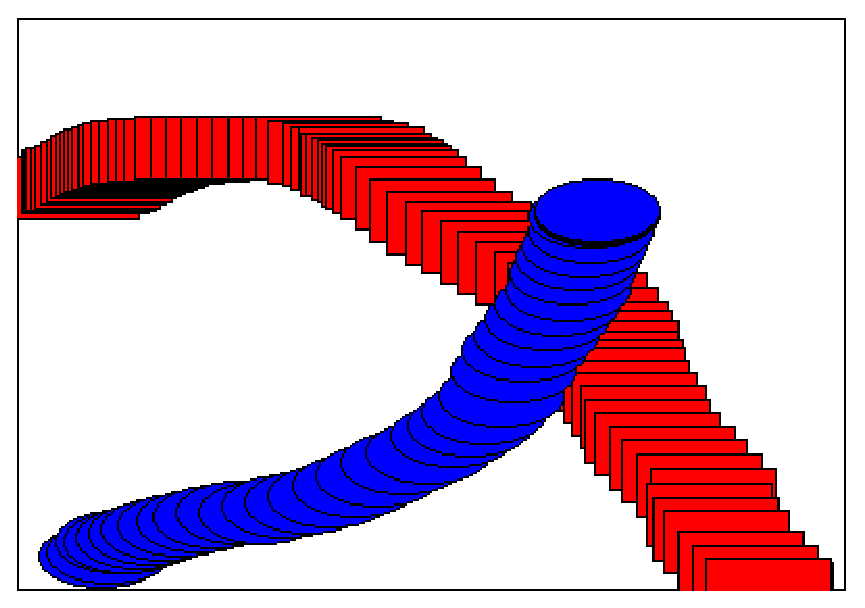
\includegraphics[scale=0.6]{images/simple-stamper-with-drag.eps}
}


The source code for the original program is \sourceref{SimpleStamper.java}.
See the discussion of dragging in Subsection~\ref{GUI1.4.4}.
(Note that the original version uses a black background, with a black border around
each shape.  That didn't work well with a lot of closely spaced shapes, so the new
version uses a white background.)

If you want to make the problem a little more challenging, when drawing shapes
during a drag operation, make sure that the shapes that are drawn are at least, say,
5 pixels apart.  To implement this, you have to keep track of the position of the
last shape that was drawn.

\exercise 
Write a program that shows a small red square and a small blue
square. The user should be able to drag either square with the mouse.
(You'll need an instance variable to remember which square the user is
dragging.) The user can drag the square out of the panel if she wants; if she
does this, there is no
way to get it back.

Note that for this exercise, you should do all the drawing in the
\code{paintComponent()} method (as indeed you should whenever possible).

\exercise 
Write a program that shows
a pair of dice.  When the user clicks on the panel in the program, the dice should be rolled
(that is, the dice should be assigned newly computed random values). Each die
should be drawn as a square showing from 1 to 6 dots. Since you have to draw
two dice, its a good idea to write a subroutine, ``\code{void drawDie(Graphics g,
int val, int x, int y)}", to draw a die at the specified \code{(x,y)}
coordinates. The second parameter, \code{val}, specifies the value that is
showing on the die. Assume that the size of the panel is 100 by 100 pixels.
Here is a picture of the panel that displays the dice:

\par\dumpfigure{
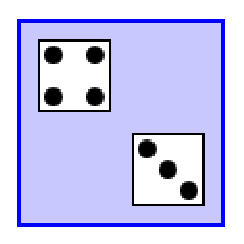
\includegraphics[scale=0.75]{images/roll-dice-gui.eps}
}


\exercise 
In Exercise~6.3,
you wrote a pair-of-dice panel where the dice are rolled when the user clicks on
the panel. Now make a pair-of-dice program in which the user rolls the
dice by clicking a button.  The button should appear under the
panel that shows the dice.  Also make the following change:  When the
dice are rolled, instead of just showing the new value, show a short animation
during which the values on the dice are changed in every frame.  The animation
is supposed to make the dice look more like they are actually rolling.

\exercise 
In Exercise~3.8, you drew a checkerboard. For this
exercise, write a program where the user can select a square by
clicking on it.  (Use a \classname{JPanel} for the checkerboard.)
Highlight the selected square by drawing a colored border around
it. When the program starts, no square is selected. When the user
clicks on a square that is not currently selected, it becomes selected (and the
previously selected square, if any, is unselected). If the
user clicks the square that is selected, it becomes unselected. Assume that the
size of the panel is exactly 160 by 160 pixels, so that each square on the
checkerboard is 20 by 20 pixels.  Here is my checkerboard, with the square in
row 3, column 3 selected:

\par\dumpfigure{
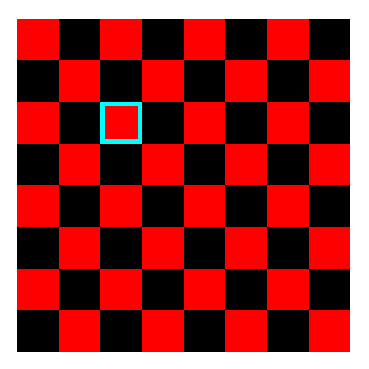
\includegraphics[scale=0.75]{images/clickable-checkerboard.eps}
}


\exercise 
For this exercise, you
should modify the SubKiller game from Subsection~\ref{GUI1.5.4}. You
can start with the existing source code, from the file 
\sourceref{SubKiller.java}. Modify the game so it
keeps track of the number of hits and misses and displays these quantities.
That is, every time the depth charge blows up the sub, the number of hits goes
up by one. Every time the depth charge falls off the bottom of the screen
without hitting the sub, the number of misses goes up by one. There is room at
the top of the panel to display these numbers. To do this exercise, you only
have to add a half-dozen lines to the source code. But you have to figure out
what they are and where to add them. To do this, you'll have to read the source
code closely enough to understand how it works.

\exercise 
Exercise~5.2 involved a class, \sourceref{StatCalc.java},
that could compute some statistics
of a set of numbers. Write a GUI program that uses the \classname{StatCalc} class to
compute and display statistics of numbers entered by the user. The panel will
have an instance variable of type \classname{StatCalc} that does the computations.
The panel should include a \classname{JTextField} where the user enters a number.
It should have four labels that display four statistics for the numbers that
have been entered: the number of numbers, the sum, the mean, and the standard
deviation. Every time the user enters a new number, the statistics displayed on
the labels should change. The user enters a number by typing it into the
\classname{JTextField} and pressing return. There should be a ``Clear" button that
clears out all the data. This means creating a new \classname{StatCalc} object and
resetting the displays on the labels. My panel also has an ``Enter" button that
does the same thing as pressing the return key in the \classname{JTextField}.
(Recall that a \classname{JTextField} generates an \classname{ActionEvent} when the
user presses return, so your panel should register itself to listen for
\classname{ActionEvents} from the \classname{JTextField} as well as the buttons.)
Here is a picture of my solution to this problem:

\par\dumpfigure{
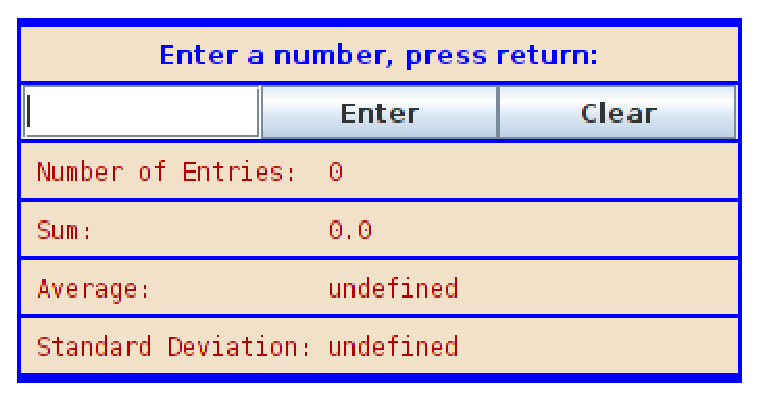
\includegraphics[scale=0.6]{images/stat-calc-gui.eps}
}


\exercise 
 Write a program that has a
\classname{JTextArea} where the user can enter some text. 
Then program should have a
button such that when the user clicks on the button, the panel will count the number
of lines in the user's input, the number of words in the user's input, and the
number of characters in the user's input. This information should be displayed
on three labels. Recall that if \code{textInput} is a
\classname{JTextArea}, then you can get the contents of the \classname{JTextArea} by
calling the function \code{textInput.getText()}. This function returns a
\classname{String} containing all the text from the text area. The number
of characters is just the length of this \classname{String}. Lines in the
\classname{String} are separated by the new line character, \code{'\1n'}, so the number of
lines is just the number of new line characters in the \classname{String}, plus
one. Words are a little harder to count. Exercise~3.4 
has some advice about finding the
words in a \classname{String}. Essentially, you want to count the number of
characters that are first characters in words. Don't forget to put your
\classname{JTextArea} in a \classname{JScrollPane},
and add the scroll pane to the container, not the text area. Scrollbars should appear when the
user types more text than will fit in the available area. Here is a picture of my solution:

\par\dumpfigure{
\includegraphics[scale=0.6]{images/text-count.eps}
}


\exercise 
 A \newword{polygon} 
is a geometric figure made up of a sequence of
connected line segments. The points where the line segments meet are called the
\newword{vertices} of the polygon. The \classname{Graphics}
class includes commands for drawing and filling polygons. For these commands,
the coordinates of the vertices of the polygon are stored in arrays. If
\code{g} is a variable of type \classname{Graphics} then


\mylist{

\myitem \codedef{g.drawPolygon(xCoords, yCoords,
pointCt)} will draw the outline of the polygon with vertices at the points
\code{(xCoords[0],yCoords[0])}, \code{(xCoords[1],yCoords[1])}, \dots,
\code{(xCoords[pointCt-1],yCoords[pointCt-1])}. The third parameter,
\code{pointCt}, is an \ptype{int} that specifies the number of vertices of
the polygon. Its value should be 3 or greater. The first two parameters are
arrays of type \code{int[]}. Note that the polygon automatically includes a
line from the last point, \code{(xCoords[pointCt-1],yCoords[pointCt-1])},
back to the starting point \code{(xCoords[0],yCoords[0])}.
\myitem \codedef{g.fillPolygon(xCoords, yCoords,
pointCt)} fills the interior of the polygon with the current drawing
color. The parameters have the same meaning as in the \code{drawPolygon()}
method. Note that it is OK for the sides of the polygon to cross each other,
but the interior of a polygon with self-intersections might not be exactly what
you expect.
}


Write a program that lets the user draw polygons.  As the user clicks a
sequence of points, count them and store their x- and y-coordinates in two
arrays. These points will be the vertices of the polygon. As the user is creating
the polygon, you should just connect all the points with line segments.
When the user clicks near the starting point, draw the complete polygon. Draw
it with a red interior and a black border.  Once the user has completed a
polygon, the next click will clear the data and start a new polygon from scratch.
All drawing should be done in the \code{paintComponent()} method.

Here is a picture of my solution after the user has drawn a fairly complex polygon:

\par\dumpfigure{
\includegraphics[scale=0.5]{images/polygon.eps}
}


\exercise 
Write a GUI Blackjack program
that lets the user play a game of Blackjack, with the computer as the dealer.
The program should draw the user's cards and the dealer's cards, just as was
done for the graphical HighLow card game in  Subsection~\ref{GUI1.7.6}.
You can use the source code for that game, \sourceref{HighLowGUI.java}, for some ideas about how to
write your Blackjack game. The structures of the HighLow panel and the
Blackjack panel are very similar. You will certainly want to use the
\code{drawCard()} method from the HighLow program.


You can find a description of the game of Blackjack in Exercise~5.5. 
Add the following rule to that
description: If a player takes five cards without going over 21, that player
wins immediately. This rule is used in some casinos. For your program, it means
that you only have to allow room for five cards. You should assume that the
panel is just wide enough to show five cards, and that it is tall enough 
show the user's hand and the dealer's hand.


Note that the design of a GUI Blackjack game is very different from the
design of the text-oriented program that you wrote for Exercise~5.5. The user
should play the game by clicking on ``Hit" and ``Stand" buttons. There should be
a ``New Game" button that can be used to start another game after one game ends.
You have to decide what happens when each of these buttons is pressed. You
don't have much chance of getting this right unless you think in terms of the
states that the game can be in and how the state can change.


Your program will need the classes defined in 
\sourceref{Card.java},
\sourceref{Hand.java},
\sourceref{Deck.java}, and
\sourceref{BlackjackHand.java}.


The next exercise has a picture of a blackjack game that
you can use a guide, except that the version for this exercise does not allow betting.


\exercise 
In the Blackjack game 
from Exercise~6.10, the user can click on the ``Hit",
``Stand", and ``NewGame" buttons even when it doesn't make sense to do so. It
would be better if the buttons were disabled at the appropriate times. The ``New
Game" button should be disabled when there is a game in progress. The ``Hit" and
``Stand" buttons should be disabled when there is not a game in progress. The
instance variable \code{gameInProgress} tells whether or not a game is in
progress, so you just have to make sure that the buttons are properly enabled
and disabled whenever this variable changes value. 
I strongly advise writing a subroutine that can be called whenever it is
necessary to set the value of the \code{gameInProgress} variable. Then the
subroutine can take responsibility for enabling and disabling the buttons.
Recall that if \code{bttn} is a variable of type \code{JButton}, then
\code{bttn.setEnabled(false)} disables the button and
\code{bttn.setEnabled(true)} enables the button.


As a second (and more difficult) improvement, make it possible
for the user to place bets on the Blackjack game. When the program starts, give
the user \$100. Add a \classname{JTextField} to the strip of controls along the
bottom of the panel. The user can enter the bet in this \classname{JTextField}.
When the game begins, check the amount of the bet. You should do this when the
game begins, not when it ends, because several errors can occur: The contents
of the \classname{JTextField} might not be a legal number, the bet that the user
places might be more money than the user has, or the bet might be \<= 0. You
should detect these errors and show an error message instead of starting the
game. The user's bet should be an integral number of dollars.


It would be a good idea to make the \classname{JTextField} uneditable while the
game is in progress. If \code{betInput} is the \classname{JTextField}, you can
make it editable and uneditable by the user with the commands
\code{betInput.setEditable(true)} and \code{betInput.setEditable(false)}.


In the \code{paintComponent()} method, you should include commands to
display the amount of money that the user has left.


There is one other thing to think about: Ideally, the program should not start a new
game when it is first created. The user should have a chance to set a bet
amount before the game starts. So, in the constructor for the drawing surface class, you
should not call \code{doNewGame()}. You might want to display a message such
as ``Welcome to Blackjack" before the first game starts.
   

Here is a picture of my program:

\par\dumpfigure{
\includegraphics[scale=0.5]{images/blackjack-gui.eps}
}

 

\end{exercises}

   



\begin{quiz}

\quizquestion 
Programs written for a
graphical user interface have to deal with ``events." Explain what is meant by
the term \textit{event.} Give at least two different examples of events, and
discuss how a program might respond to those events.
\quizquestion 
Explain carefully what the
\code{repaint()} method does.
\quizquestion 
Java has a standard class
called \classname{JPanel}. Discuss \textbf{two} ways in which JPanels can be
used.
\quizquestion 
Draw the picture that will
be produced by the following \code{paintComponent()} method:
\displaycode{public static void paintComponent(Graphics g) \{
    super.paintComponent(g);
    for (int i=10; i \<= 210; i = i + 50)
       for (int j = 10; j \<= 210; j = j + 50)
          g.drawLine(i,10,j,60);
\}}\donedisplaycode

\quizquestion 
Suppose you would like a
panel that displays a green square inside a red circle, as illustrated. Write
a \code{paintComponent()} method for the panel class that will draw the image.

\par\dumpfigure{
\includegraphics[scale=0.8]{images/square-in-circle.eps}
}

\quizquestion 
Java has a standard class
called \classname{MouseEvent}. What is the purpose of this class? What does an
object of type \classname{MouseEvent} do?
\quizquestion 
One of the main classes in
Swing is the \classname{JComponent} class. What is meant by a component? What are
some examples?
\quizquestion 
 What is the function of a
\classname{LayoutManager} in Java?
\quizquestion 
Consider the illustration of nested panels from the beginning of Section~\ref{GUI1.7}.
What type of layout manager is being used for each of the three panels
in that picture?

\quizquestion 
Explain how \classname{Timers}
are used to do animation.
\quizquestion 
What is a \classname{JCheckBox}
and how is it used?
\quizquestion 
How is the \textit{preferred size} of a component set, and how is it used?

\end{quiz}


\chapter{Arrays and ArrayLists}\label{arrays}

   




\start{{\Large C}omputers get a lot of their power} from working
with \newword{data structures}. A data structure is an
organized collection of related data. An object is a data structure, but this
type of data structure---consisting of a fairly small number of named instance
variables---is just the beginning. In many cases, programmers build
complicated data structures by hand, by linking objects together. We'll look at
these custom-built data structures in Chapter~\ref{recursion}. But there is one type of
data structure that is so important and so basic that it is built into every
programming language: the array.


You have already encountered arrays in Section~\ref{control.7a}
and Subsection~\ref{OOP.1.4}.  We continue the study of arrays in this chapter,
including some new details of their use and some additional array-processing
techniques.  In particular, we will look at the important topic of algorithms for
searching and sorting an array.


An array has a fixed size that can't be changed after the array is created.
But in many cases, it is useful to have a data structure that can grow and shrink
as necessary.  In this chapter, we will look at a standard class, 
\classname{ArrayList}, that represents such a data structure.


   



\section{Array Details}\label{arrays.1}

   
   

\start{{\Large A}rray basics have been discussed} in previous chapters,
but there are still details of Java syntax to be filled in, and there is a lot more to say
about using arrays.  This section looks at some of the syntactic details, 
with more information about array processing to come in the rest of the
chapter.
   

To briefly review some of the basics\dots.  An array is a numbered sequence
of \textit{elements}, and each element acts like a separate variable.  All of the
elements are of the same type, which is called the \textit{base type} of the array.
The array as a whole also has a type.  If the base type is \classname{btype},
then the array is of type \atype{btype\hbox{[\hskip2pt]}}.  Each element in the array
has an \textit{index}, which is just its numerical position in the sequence of elements.
If the array is \code{A}, then the i-th element of the array is \code{A[i]}.
The number of elements in an array is called its \textit{length}.  The length of
an array \code{A} is \code{A.length}.  The length of an array can't
be changed after the array is created.  The elements of the array \code{A}
are \code{A[0]}, \code{A[1]}, \dots, \code{A[A.length-1]}.
An attempt to refer to an array element with an index outside the range
from zero to \code{A.length-1} causes an \classname{ArrayIndexOutOfBoundsException}.



Arrays in Java are objects, so an array variable can only refer to an array,
it does not contain the array.  The value of an array variable can also be \code{null}.
In that case, it does not refer to any array, and an attempt to refer to an
array element such as \code{A[i]} will cause a \classname{NullPointerException}.
Arrays are created using a special form of the \code{new} operator. For
example,

\displaycode{int[] A = new int[10];}\donedisplaycode


\noindent creates a new array with base type \ptype{int} and length 10, and it sets
the variable \code{A} to refer to the newly created array.



\subsection{For-each Loops}\label{arrays.1.1}
   


Arrays are often processed using \code{for} loops.  A \code{for}
loop makes it easy to process each element in an array from beginning to end.  For
example, if \code{namelist} is an array of \classname{Strings}, 
then all the values in the list can be printed using

\displaycode{for (int i = 0; i \< namelist.length; i++) \{
    System.out.println( namelist[i] );
\}}\donedisplaycode



This type of processing is so common that there is an alternative form of
the \code{for} loop that makes it easier to write.  The alternative
is called a \newword{for-each loop}.   It is probably easiest to
start with an example.  Here is a for-each loop for printing all the values
in an array of \classname{Strings}:

\displaycode{for ( String name : namelist ) \{
    System.out.println( name );
\}}\donedisplaycode


\noindent The meaning of ``\code{for (String name : namelist)}" is
``for each string, name, in the array, namelist, do the following".  The effect
is that the variable \code{name} takes on each of the values in \code{namelist}
in turn, and the body of the loop is executed for each of those values.  Note that
there is no array index in the loop.  The loop control variable, \code{name},
represents one of the values in the array, not the index of one of the values.



The for-each loop is meant specifically for processing all the values
in a data structure, and we will see in Chapter~\ref{generics} that it applies to other
data structures besides arrays.  The for-each loop makes it possible to process the
values without even knowing the details of how the data is structured.  In the
case of arrays, it lets you avoid the complications of using array indices.


A for-each loop
will perform the same operation for each value that is stored
in an array.  
If \code{itemArray} is an array of type \atype{BaseType\hbox{[\hskip2pt]}},
then a for-each loop for \code{anArray} has the form:
   
\displaycode{for ( BaseType item : itemArray ) \{
   .
   .  // process the item
   .
\}}\donedisplaycode

   
\noindent As usual, the braces are optional if there is only one statement inside the loop.
In this loop, \code{item} is the loop control variable.  It is
declared as a variable of type \classname{BaseType}, where
\classname{BaseType} is the base type of the array.  (In a
for-each loop, the loop control variable \textbf{must} be declared in the
loop; it cannot be a variable that already exists outside the loop.)  
When this loop is executed, each value from the array is assigned
to \code{item} in turn and the body of the loop is executed for each
value.  Thus, the above loop is exactly equivalent to:
   
\displaycode{for ( int index = 0; index \< itemArray.length; index++ ) \{
   BaseType item;
   item = itemArray[index];  // Get one of the values from the array
     .
     .  // process the item
     .  
\}}\donedisplaycode

   

For example, if \code{A} is an array of type \atype{int\hbox{[\hskip2pt]}}, then
we could print all the values from \code{A} with the for-each loop:
   
\displaycode{
for ( int item : A )
   System.out.println( item );
}\donedisplaycode


\noindent and we could add up all the positive integers in \code{A} with:
   
\displaycode{int sum = 0;   // This will be the sum of all the positive numbers in A
for ( int item : A ) \{
   if (item \> 0)
      sum = sum + item;
\}}\donedisplaycode

   

The for-each loop is not always appropriate.  For example, there is no
simple way to use it to process the items in just a part of an array, or to
process the elements in reverse order.
However, it does make the code a little simpler when you do want to process all the values, in order.
since it eliminates any need to use array indices.   
   

It's important to note that a for-each loop processes the \textbf{values} in
the array, not the \textbf{elements} (where an element means the actual memory
location that is part of the array).  For example, consider the following
incorrect attempt to fill an array of integers with 17's:
   
\displaycode{int[] intList = new int[10];
for ( int item : intList ) \{   \newcode{// INCORRECT! DOES NOT MODIFY THE ARRAY!}
   item = 17;
\}}\donedisplaycode

   
\noindent The assignment statement \code{item = 17} assigns the value 17 to
the loop control variable, \code{item}.  However, this has nothing to
do with the array.  When the body of the loop is executed, the
value from one of the elements of the array is copied into \code{item}.
The statement \code{item~=~17} replaces that copied value
but has no effect on the array element from which it was copied; the
value in the array is not changed.  The loop is equivalent to
  
\displaycode{int[] intList = new int[10];
for ( int i = 0; i \< intList.length; i++ ) \{
   int item = intList[i];
   item = 17;
\}}\donedisplaycode

   
\noindent which certainly does not change the value of any element in the array.


   
\subsection{Variable Arity Methods}\label{arrays.1.2}



Before Java 5, every method in Java had a fixed arity.
(The \newword{arity} of a method is defined as the number
of parameters in a call to the method.)  In a fixed arity method, the number
of parameters must be the same in every call to the method and must be the same
as the number of formal parameters in the method's definition.  Java~5 introduced
\newword{variable arity methods}.  In a variable arity method, different
calls to the method can have different numbers of parameters.  For example,
the formatted output method \code{System.out.printf}, which was introduced
in Subsection~\ref{basics.4.1}, is a variable arity method.  The first
parameter of \code{System.out.printf} must be a \classname{String},
but it can have any number of additional parameters, of any types.


Calling a variable arity method is no different from calling any other
sort of method, but writing one requires some new syntax.  As an example,
consider a method that can compute the average of any number of values of
type \ptype{double}.  The definition of such a method could begin
with:
   
\displaycode{public static double average( double...  numbers ) \{}\donedisplaycode

   
\noindent Here, the \code{...} after the type name, \code{double}, 
is what makes this a variable arity method.  It indicates
that any number of values of type \ptype{double} can be provided when
the subroutine is called, so that for example \code{average(1,4,9,16)}, 
\code{average(3.14,2.17)}, \code{average(0.375)}, and even
\code{average()} are all legal calls to this method.  Note that 
actual parameters of type \ptype{int} can be passed to \code{average}.
The integers will, as usual, be automatically converted to real numbers.


When the method is called, the values of all the actual parameters
that correspond to the variable arity parameter are placed into an array,
and it is this array that is actually passed to the method.  That is,
in the body of a method, a variable arity parameter of type
\classname{T} actually looks like an ordinary parameter of type
\atype{T\hbox{[\hskip2pt]}}.  The length of the array tells you how many actual parameters
were provided in the method call.  In the \code{average} example, the body
of the method would see an array named \code{numbers} of type \atype{double\hbox{[\hskip2pt]}}.
The number of actual parameters in the method call would be \code{numbers.length},
and the values of the actual parameters would be \code{numbers[0]},
\code{numbers[1]}, and so on.  A complete definition of the method would be:

   
\displaycode{public static double average( double... numbers ) \{
        // Inside this method, numbers if of type double[].
   double sum;      // The sum of all the actual parameters.
   double average;  // The average of all the actual parameters.
   sum = 0;
   for (int i = 0; i \< numbers.length; i++) \{
      sum = sum + numbers[i];  // Add one of the actual parameters to the sum.
   \}
   average = sum / numbers.length;
   return average;
\}}\donedisplaycode




By the way, it is possible to pass a single array
to a variable arity method, instead of a list of individual values.  For example, suppose that
\code{salesData} is a variable of type \atype{double\hbox{[\hskip2pt]}}. Then
it would be legal to call \code{average(salesData)}, and this would compute
the average of all the numbers in the array.


The formal parameter list in the definition of a variable-arity method can 
include more than one parameter, but the \code{...} can only be applied to the
very last formal parameter.
   

As an example, consider a method that can draw a polygon through
any number of points.  The points are given as values of type \classname{Point},
where an object of type \classname{Point} has two instance variables,
\code{x} and \code{y}, of type \ptype{int}.
In this case, the method has one ordinary parameter---the
graphics context that will be used to draw the polygon---in addition to the
variable arity parameter.  Remember that inside the definition of the
method, the parameter \code{points} becomes an array of 
\classname{Points}:
   
\displaycode{public static void drawPolygon(Graphics g, Point... points) \{
    if (points.length \> 1) \{  // (Need at least 2 points to draw anything.)
       for (int i = 0; i \< points.length - 1; i++) \{
           // Draw a line from i-th point to (i+1)-th point
           g.drawLine( points[i].x, points[i].y, points[i+1].x, points[i+1].y );
       \}
       // Now, draw a line back to the starting point.
       g.drawLine( points[points.length-1].x, points[points.length-1].y,
                       points[0].x, points[0].y );
    \}
\}}\donedisplaycode


\noindent When this method is called, the subroutine call statement must have one actual parameter
of type \classname{Graphics}, which can be followed by any number of
actual parameters of type \classname{Point}.
   

For a final example, let's look at a method that strings together all of the
values in a list of strings into a single, long string.  This example uses a for-each
loop to process the array:

\displaycode{public static String concat( String... values ) \{
   StringBuffer buffer;  // Use a StringBuffer for more efficient concatenation.
   buffer = new StringBuffer();  // Start with an empty buffer.
   for ( String str : values ) \{ // A "for each" loop for processing the values.
       buffer.append(str); // Add string to the buffer.
   \}
   return buffer.toString(); // return the contents of the buffer
\}}\donedisplaycode


\noindent Given this method definition, \code{concat("Hello", "World")}
would return the string ``HelloWorld", and \code{concat()} would
return an empty string. Since a variable arity method can also accept an
array as actual parameter, we could also call \code{concat(lines)}
where \code{lines} is of type \atype{String\hbox{[\hskip2pt]}}.  This would 
concatenate all the elements of the array into a single string.


   
\subsection{Array Literals}\label{arrays.1.3}

  

We have seen that it is possible to initialize an array variable 
with a list of values at the time it is declared.
For example,

\displaycode{int[] squares = \{ 1, 4, 9, 16, 25, 36, 49 \};}\donedisplaycode


\noindent This initializes \code{squares} to refer to a newly created array
that contains the seven values in the list



A list initializer of this form can be used \textbf{only} in a declaration
statement, to give an initial value to a newly declared array variable. It
cannot be used in an assignment statement to assign a value to a variable that
already existed. However, there is another, similar notation for
creating a new array that can be used in other places. The notation uses 
another form of the \code{new}
operator to both create a new array object and fill it with values.
(The rather odd syntax
is similar to the syntax for anonymous inner classes, which were discussed in
Subsection~\ref{OOP.8.3}.) As an example, to assign a new value to
an array variable, \code{cubes}, of type \atype{int\hbox{[\hskip2pt]}}, you could
use:

\displaycode{cubes = new int[] \{ 1, 8, 27, 64, 125, 216, 343 \};}\donedisplaycode


\noindent This is an assignment statement rather than a declaration, so the
array initializer syntax, without ``\code{new int[]}," would not
be legal here.  The general syntax for this form of the 
\code{new} operator is

\displaycode{new \bnf{base-type} [ ] \{ \bnf{list-of-values} \}}\donedisplaycode


\noindent This is actually an expression whose value is a reference to a newly created
array object.  In this sense, it is an ``array literal," since it is something that you can type
in a program to represent a value. This means that it can be used in any
context where an object of type \bnf{base-type}\code{[]} is legal.
For example, you could pass the newly created array as an actual parameter to
a subroutine.  Consider the following utility method for creating a menu
from an array of strings:

\displaycode{/**
 * Creates a JMenu.  The names for the JMenuItems in the menu are
 * given as an array of strings.
 * @param menuName  the name for the JMenu that is to be created.
 * @param handler  the listener that will respond to items in the menu.
 *    This ActionListener is added as a listener for each JMenuItem.
 * @param itemNames  an array holding the text that appears in each
 *     JMenuItem.  If a null value appears in the array, the corresponding
 *     item in the menu will be a separator rather than a JMenuItem.
 * @return  the menu that has been created and filled with items.
 */
public static JMenu createMenu( 
            String menuName, ActionListener handler, String[] itemNames ) \{
    JMenu menu = new JMenu(menuName);
    for ( String itemName : itemNames ) \{
        if ( itemName == null ) \{
            menu.addSeparator();
        \}
        else \{
            JMenuItem item = new JMenuItem(itemName);
            item.addActionListener(handler);
            menu.add(item);
        \}
    \}
    return menu;
\}
}\donedisplaycode


\noindent The third parameter in a call to \code{createMenu} is an array of 
strings.  The array that is passed as an actual parameter could be created
in place, using the \code{new} operator.  For example, assuming
that \code{listener} is of type \classname{ActionListener},
we can use the following statement to create an entire File menu:

\displaycode{JMenu fileMenu = createMenu( "File", listener
              \newcode{new String[] \{ "New", "Open", "Close", null, "Quit" \}} );}\donedisplaycode

   
\noindent This should convince you that
being able to create and use an array ``in place" in this way can be very convenient,
in the same way that anonymous inner classes are convenient.
   

By the way, it is perfectly legal to use the ``\code{new BaseType[] \{~\dots~\}}" syntax
instead of the array initializer syntax in the declaration of an array variable.  For example,
instead of saying:
   
\displaycode{int[] primes = \{ 2, 3, 5, 7, 11, 13, 17, 19 \};}\donedisplaycode

   
\noindent you can say, equivalently,
   
\displaycode{int[] primes = new int[] \{ 2, 3, 5, 7, 11, 17, 19 \};}\donedisplaycode

   
\noindent In fact, rather than use a special notation that works only in the context
of declaration statements, I sometimes prefer to use the second form.


\mybreak



One final note: For historical reasons, an array declaration such as

\displaycode{int[] list;}\donedisplaycode


\noindent can also be written as
   
\displaycode{int list[];}\donedisplaycode


\noindent which is a syntax used in the languages C and C++. However, this alternative
syntax does not really make much sense in the context of Java, and it is
probably best avoided. After all, the intent is to declare a variable of a
certain type, and the name of that type is ``\atype{int\hbox{[\hskip2pt]}}". It makes sense to
follow the ``\bnf{type-name}  \bnf{variable-name};" syntax for such declarations.
  




   



\section{Array Processing}\label{arrays.2}

   
   

\start{{\Large M}ost examples of array processing} that we
have looked at have actually been fairly straightforward: processing
the elements of the array in order from beginning to end, or random
access to an arbitrary element of the array.  In this section
and later in the chapter, you'll see some of the more interesting
things that you can do with arrays.
 
\subsection{Some Processing Examples}\label{arrays.2.1}
   


To begin, here's an example to remind you to be careful about
avoiding array indices outside the legal range.  Suppose that
\code{lines} is an array of type \code{String[]},
and we want to know whether \code{lines} contains any
duplicate elements in consecutive locations.  That is, we
want to know whether \code{lines[i].equals(lines[i+1])}
for any index~\code{i}.  Here is a failed attempt
to check that condition:

\displaycode{boolean dupp = false;  // Assume there are no duplicates
for ( int i = 0; i \< list.length; i++ ) \{
    if ( lines[i].equals(lines[i+1]) ) \{  // \newcode{THERE IS AN ERROR HERE!}
        dupp = true;   // we have found a duplicate!
        break;
    \}
\}}\donedisplaycode


\noindent This \code{for} loop looks like many others that we have written,
so what's the problem?  The error occurs when \code{i} takes on
its final value in the loop, \code{i} equal to \code{lines.length-1}.
In that case, \code{i+1} is equal to \code{lines.length}.  But
the last element in the array has index \code{lines.length-1},
so \code{lines.length} is not a legal index.  This means that the
reference to \code{lines[i+1]} causes an ArrayIndexOutOfBoundsException.
This is easy to fix; we just need to stop the loop before \code{i+1}
goes out of range:

\displaycode{boolean dupp = false;  // Assume there are no duplicates
for ( int i = 0; i \< \newcode{list.length - 1 }; i++ ) \{
    if ( lines[i].equals(lines[i+1]) ) \{ 
        dupp = true;   // we have found a duplicate!
        break;
    \}
\}}\donedisplaycode



This type of error can be even more insidious when working with partially full
arrays (see Subsection~\ref{control.7a.4}), where usually only part of the array is in
use, and a counter is used to keep track of how many spaces in the array are used.
With a partially full array, the problem
is not looking beyond the end of the array, but looking beyond \textit{the part of the array
that is in use}.  When your program tries to look beyond the end of an array, at
least the program will crash to let you know that there is a problem.  With a 
partially full array, the problem can go undetected.


\mybreak




For the next  example, let's continue with partially full arrays.  We have seen how to add
an item to a partially full array, but suppose that we also want to be able to
remove items?  Suppose that you write a game
program, and that players can join the game and leave the game as it
progresses. As a good object-oriented programmer, you probably have a class
named \classname{Player} to represent the individual players in the game. A list
of all players who are currently in the game could be stored in an array,
\code{playerList}, of type \atype{Player\hbox{[\hskip2pt]}}. Since the number of players can
change, you will follow the partially full array pattern, and
you will need a variable, \code{playerCt}, to record the number
of players currently in the game. Assuming that there will never be more than
10 players in the game, you could declare the variables as:

\displaycode{Player[] playerList = new Player[10];  // Up to 10 players.
int      playerCt = 0;  // At the start, there are no players.}\donedisplaycode



After some players have joined the game, \code{playerCt} will be greater
than 0, and the player objects representing the players will be stored in the
array elements \code{playerList[0]}, \code{playerList[1]}, \dots,
\code{playerList[playerCt-1]}. Note that the array element
\code{playerList[playerCt]} is \textbf{not} in use. The procedure for
adding a new player, \code{newPlayer}, to the game is simple:

\displaycode{playerList[playerCt] = newPlayer; // Put new player in next
                                  //     available spot.
playerCt++;  // And increment playerCt to count the new player.}\donedisplaycode



But deleting a player from the game is a little harder, since you don't want to
leave a ``hole" in the array where the deleted player used to be. 
Suppose you want to delete the player at index
\code{k} in \code{playerList}.  The number of players goes down
by one, so one fewer space is used in the array.  
If you are not worried about keeping the
players in any particular order, then one way to do this is to move the player
from the last occupied position in the array
into position \code{k} and then
to decrement the value of \code{playerCt}:

\displaycode{playerList[k] = playerList[playerCt - 1];
playerCt--;}\donedisplaycode


\noindent The player previously in position \code{k} is no longer in the array, so
we have deleted that player from the list.  The
player previously in position \code{playerCt~-~1} is now in the array twice.
But it's only in the occupied or valid part of the array once, since
\code{playerCt} has decreased by one. Remember that every element of the
array has to hold some value, but only the values in positions 0 through
\code{playerCt~-~1} will be looked at or processed in any way.
(By the way, you should think about what happens if the player that is being deleted
is in the last position in the list.  The code does still work in this case.  What
exactly happens?)


Suppose that when deleting the player in position \code{k}, you'd like to
keep the remaining players in the same order. (Maybe because they take turns in
the order in which they are stored in the array.) To do this, all the players
in positions \code{k+1} and above must move down one position in the array.
Player \code{k+1} replaces player \code{k}, who is out of the game. Player
\code{k+2} fills the spot left open when player \code{k+1} is moved. And so
on. The code for this is

\displaycode{for (int i = k+1; i \< playerCt; i++) \{
    playerList[i-1] = playerList[i];
\}
playerCt--;}\donedisplaycode



Here is an illustration of the two ways of deleting an item from a partially full
array.  Here, player ``C" is being deleted:


\par\dumpfigure{
\includegraphics[scale=0.6]{images/delete-from-array.eps}
}

    

\mybreak



This leaves open the question of what happens when a partially full array
becomes full, but you still want to add more items to it?  We can't change
the size of the array---but we can make a new, bigger array and copy the data
from the old array into the new array.  But what does it mean to copy an
array in the first place?


Suppose that \code{A} and \code{B} are array variables, with the same base type,
and that \code{A} already refers to an array.  Suppose that we want \code{B} to
refer to a copy of \code{A}.  The first thing to note is that
the assignment statement

\displaycode{B = A;}\donedisplaycode


\noindent does \textbf{not} make a copy of \code{A}.  Arrays are objects, and array variable can only
hold a pointer to an array. The assignment statement copies the pointer from \code{A}
into \code{B}, and the result is that \code{A} and \code{B} now point
to the same array.  For example, \code{A[0]} and \code{B[0]} are just
different names for exactly the same array element.  To make \code{B} refer to
a copy of \code{A}, we need to make an entirely new array and copy all the items from
\code{A} into \code{B}.  Let's say that \code{A} and \code{B}
are of type \atype{double\hbox{[\hskip2pt]}}.  Then to make a copy of \code{A}, we can say

\displaycode{double B;
B = new double[A.length];  // Make a new array with the same length as A.
for ( int i = 0; i \< A.length; i++ ) \{
    B[i] = A[i];
\}}\donedisplaycode



To solve the problem of adding to a partially full array that has become full,
we just need to make a new array that is bigger than the existing array.  The usual
choice is to make a new array twice as big as the old.  We need to meet one
more requirement:  At the end, the variable that referred to the old array
must now point to the new array.  That variable is what gives us access to the
data, and at the end that data is in the new array.  Fortunately, a simple
assignment statement will make the variable point to the correct array.
Let's suppose that we are using \code{playerList} and \code{playerCt}
to store the players in a game, as in the example above, and we want to add
\code{newPlayer} to the game.  Here is how we can do that even if the
\code{playerList} array is full:

\displaycode{if ( playerCt == playerList.length ) \{
        // The number of players is already equal to the size of the array.
        // The array is full.  Make a new array that has more space.
    Player[] temp;   // A variable to point to the new array.
    temp = new Player[ 2*playerList.length ];  // Twice as big as the old array.
    for ( int i = 0; i \< playerList.length; i++ ) \{
        temp[i] = playerList[i];  // Copy item from old array into new array.
    \}
    playerList = temp;  // playerList now points to the new, bigger array.    
\}
// At this point, we know that there is room in the array for newPlayer.
playerList[playerCt] = newPlayer;
playerCt++;
}\donedisplaycode


\noindent After the new array has been created, there is no longer any variable that
points to the old array, so it will be garbage collected.

   

\subsection{Some Standard Array Methods}\label{arrays.2.2}



Copying an array seems like such a common method that you might expect
Java to have a built-in method already defined to do it.  In fact,
Java comes with several standard array-processing methods.  The
methods are defined as \code{static} methods in a class
named \classname{Arrays}, which is in the package \code{java.util}.
For example, for any array, \code{list},
   
\displaycode{Arrays.copyOf( list, lengthOfCopy )}\donedisplaycode


\noindent is a function that returns a new array whose length is given by \code{lengthOfCopy},
containing items copied from \code{list}.  If \code{lengthOfCopy} is greater
than \code{list.length}, then extra spaces in the new array will have their default
value (zero for numeric arrays, \code{null} for object arrays, and so on).
If \code{lengthOfCopy} is less than or equal to \code{list.length}, then
only as many items are copied from \code{list} as will fit in the new array.
So if \code{A} is any array, then

\displaycode{B = Arrays.copyOf( A, A.length );}\donedisplaycode


\noindent sets \code{B} to refer to an exact copy of \code{A}, and

\displaycode{playerList = Arrays.copyOf( playerList, 2*playerList.length );}\donedisplaycode


\noindent could be used to double the amount of space available in a partially full array with
just one line of code.
We can also use \code{Arrays.copyOf} to decrease the size of a partially full array.
We might want to do that to avoid having a lot of excess, unused spaces.  To implement
this idea, the code for deleting player number \code{k} from the list of players
might become

\displaycode{playerList[k] = playerList[playerCt-1];
playerCt--;
if ( playerCt \< playerList.length/2 ) \{
        // More than half the spaces are empty. Cut the array size in half.
    playerList = Arrays.copyOf( playerList, playerList.length/2 );
\}}\donedisplaycode



I should mention that class \classname{Arrays} actually contains a bunch
of \code{copyOf} methods, one for each of the primitive types and one for
objects.  I should also note that when an array of objects is copied, it is only
pointers to objects that are copied into the new array.  The contents of the
objects are not copied.  This is the usual rule for assignment of pointers.


\mybreak



The \classname{Arrays} class contains other useful methods.  I'll mention
a few of them.  As with \code{Arrays.copyOf}, there are actually multiple versions
of all of these methods, for different array types.



\mylist{

\myitem \codedef{Arrays.fill( array, value )} --- Fill an entire array with
a specified value.  The type of \code{value} must be compatible with  the base type of
the \code{array}.  For example, assuming that \code{numlist} is an array
of type \atype{double\hbox{[\hskip2pt]}}, then \code{Arrays.fill(numlist,17)} will set
every element of \code{numlist} to have the value 17.
\myitem \codedef{Arrays.fill( array, fromIndex, toIndex, value )} --- Fills part
of the \code{array} with \code{value}, starting at index number \code{fromIndex}
and ending with index number \code{toIndex-1}.  Note that \code{toIndex} itself 
is not included.
\myitem \codedef{Arrays.toString( array )} --- A function that returns a \classname{String}
containing all the values from \code{array}, separated by commas and enclosed between
square brackets. The values in the array are converted into strings in the same way
they would be if they were printed out.
\myitem \codedef{Arrays.sort( array )} --- Sorts the entire array.  To sort an 
array means to rearrange the values in the array so that they are in increasing order.
This method works for arrays of \classname{String} and arrays of primitive type values
(except for \ptype{boolean}, which would be kind of silly).  But it does not work
for all arrays, since it must be meaningful to compare any two values in the array, to
see which is ``smaller."  We will discuss array-sorting algorithms in Section~\ref{arrays.4}.
\myitem \codedef{Arrays.sort( array, fromIndex, toIndex )} --- Sorts just
the elements from \code{array[fromIndex]} up to \code{array[toIndex-1]}
\myitem \codedef{Arrays.binarySearch( array, value )} --- Searches for \code{value}
in the \code{array}.  The array must already be sorted into increasing order.
This is a function that returns an \ptype{int}.  If the value is found in the array,
the return value is the index of an element that contains that value.  If the value does not
occur in the array, the return value is~-1.  We will discuss the binary search algorithm
in Section~\ref{arrays.4}.
}







\subsection{RandomStrings Revisited}\label{arrays.2.3}

   

One of the examples in Subsection~\ref{GUI1.4.2} was a GUI program
that shows multiple copies of a message in random positions, colors, and fonts.
When the user clicks the program window, the positions, colors, and fonts are
changed to new random values. Like several other examples from that chapter,
the program had a flaw: It didn't have any way of storing the data that it would
need to redraw itself.  Arrays provide us with one possible solution to this
problem.  We can write a new version of RandomStrings that uses
an array to store the position, font, and color of each string. When the panel
is painted, this information is used to draw the strings,
so that the panel will paint itself correctly whenever it has to be redrawn.
When the user clicks, the array is filled with new
random values and the panel is repainted using the new data.  So, the
only time that the picture will change is in response to a mouse click.
The new version of the program is \sourceref{RandomStringsWithArray.java}.



In the program, the number of copies of the message is given by a named
constant, \code{MESSAGE\_COUNT}. One way to store the position, color, and
font of \code{MESSAGE\_COUNT} strings would be to use four arrays:

\displaycode{int[] x = new int[MESSAGE\_COUNT];  
int[] y = new int[MESSAGE\_COUNT];
Color[] color = new Color[MESSAGE\_COUNT];
Font[] font = new Font[MESSAGE\_COUNT];}\donedisplaycode


\noindent These arrays would be filled with random values. In the
\code{paintComponent()} method, the \code{i}-th copy of the string would be
drawn at the point \code{(x[i],y[i])}. Its color would be given by
\code{color[i]}. And it would be drawn in the font \code{font[i]}. This
would be accomplished by the \code{paintComponent()} method

\displaycode{public void paintComponent(Graphics g) \{
   super.paintComponent(); // (Fill with background color.)
   for (int i = 0; i \< MESSAGE\_COUNT; i++) \{
      g.setColor( color[i] );
      g.setFont( font[i] );
      g.drawString( message, x[i], y[i] );
   \}
\}}\donedisplaycode


\noindent This approach is said to use \newword{parallel arrays}.
The data for a given copy of the message is spread out across several arrays.
If you think of the arrays as laid out in parallel columns---array \code{x}
in the first column, array \code{y} in the second, array \code{color} in
the third, and array \code{font} in the fourth---then the data for the
\code{i}-th string can be found along the \code{i}-th row. There is
nothing wrong with using parallel arrays in this simple example, but it does go
against the object-oriented philosophy of keeping related data in one object.
If we follow this rule, then we don't have to \textbf{imagine} the relationship
among the data, because all the data for one copy of the message is physically
in one place. So, when I wrote the program, I made a simple class to represent
all the data that is needed for one copy of the message:

\displaycode{/**
 * An object of this type holds the position, color, and font
 * of one copy of the string.
 */
private static class StringData \{
   int x, y;     // The coordinates of the left end of baseline of string.
   Color color;  // The color in which the string is drawn.
   Font font;    // The font that is used to draw the string.
\}}\donedisplaycode


\noindent To store the data for multiple copies of the message, I use an array of
type \atype{StringData\hbox{[\hskip2pt]}}. The array is declared as an instance variable, with
the name \code{stringData}:

\displaycode{StringData[] stringData;}\donedisplaycode


\noindent Of course, the value of \code{stringData} is \code{null} until an actual array
is created and assigned to it. The array has to be created and filled with data.
Furthermore, each element of the array is an object of type \classname{StringData}
which has to be created before it can be used.  The following subroutine is used to
create the array and fill it with random data:

\displaycode{private void createStringData() \{
    int width = getWidth();
    int height = getHeight();
    stringData = new StringData[MESSAGE\_COUNT];
    for (int i = 0; i \< MESSAGE\_COUNT; i++) \{
            // Create an object to represent the data for string number i,
            // and fill it with random values.
        stringData[i] = new StringData();
        int fontIndex = (int)(Math.random() * 5);
        stringData[i].font = fonts[fontIndex]; // one of 5 fonts, selected at random
        float hue = (float)Math.random();
        stringData[i].color = Color.getHSBColor(hue, 1.0F, 1.0F);  // random color
        stringData[i].x = -50 + (int)(Math.random()*(width+40));  // random x-coord
        stringData[i].y = (int)(Math.random()*(height+20));  // random y-coord
    \}
\}}\donedisplaycode




This method is called before the panel is painted for the first time.  It is also called
when the user clicks the panel with the mouse, so that a mouse click will cause new random
data to be created.  Those are the only times when the picture can change.  For example,
resizing the window will cause \code{paintComponent()} to be called, but since the
data hasn't changed, \code{paintComponent()} will just redraw the same picture.
Here is the code from \code{paintComponent()} that draws all the strings, using the
data from the array:

\displaycode{for (int i = 0; i \< MESSAGE\_COUNT; i++) \{
    g.setColor( \newcode{stringData[i].}color );
    g.setFont( \newcode{stringData[i].}font );
    g.drawString( message, \newcode{stringData[i].}x, \newword{stringData[i].}y );
\}}\donedisplaycode

   
\noindent Note that I could also have used a for-each loop here, which might be easier
to understand:
   
\displaycode{for ( StringData data : stringData ) \{
    g.setColor( data.color );
    g.setFont( data.font );
    g.drawString( message, data.x, data.y );
\}}\donedisplaycode

   
\noindent In this loop, the loop control variable, \code{data}, holds a copy of one
of the values from the array.  That value is a reference to an object of type
\classname{StringData}, which has instance variables named
\code{color}, \code{font}, \code{x}, and \code{y}.
Once again, the use of a for-each loop has eliminated the need to work with
array indices.



\mybreak



RandomStringsWithArray uses one other array of objects. The font for a given copy of the
message is chosen at random from a set of five possible fonts. In the original
version, there were five variables of type \classname{Font} to
represent the fonts. The variables were named \code{font1}, \code{font2},
\code{font3}, \code{font4}, and \code{font5}. To select one of these
fonts at random, a \code{switch} statement can be used:

\displaycode{Font randomFont;  // One of the 5 fonts, chosen at random.
int rand;         // A random integer in the range 0 to 4.

fontNum = (int)(Math.random() * 5);
switch (fontNum) \{
   case 0:
      randomFont = font1;
      break;
   case 1:
      randomFont = font2;
      break;
   case 2:
      randomFont = font3;
      break;
   case 3:
      randomFont = font4;
      break;
   case 4:
      randomFont = font5;
      break;
\}}\donedisplaycode


\noindent In the new version of the program, the five fonts are stored in an array,
which is named \code{fonts}. This array is declared as an instance
variable of type \atype{Font\hbox{[\hskip2pt]}}

\displaycode{Font[] fonts;}\donedisplaycode


\noindent The array is created in the constructor, and each element of the array is set
to refer to a new \classname{Font} object:

\displaycode{fonts = new Font[5];  // Create the array to hold the five fonts.
 
fonts[0] = new Font("Serif", Font.BOLD, 14);
fonts[1] = new Font("SansSerif", Font.BOLD + Font.ITALIC, 24);
fonts[2] = new Font("Monospaced", Font.PLAIN, 20);
fonts[3] = new Font("Dialog", Font.PLAIN, 30);
fonts[4] = new Font("Serif", Font.ITALIC, 36);}\donedisplaycode


\noindent This makes it much easier to select one of the fonts at random. It can be
done with the statements

\displaycode{Font randomFont;  // One of the 5 fonts, chosen at random.
int fontIndex;    // A random number in the range 0 to 4.
fontIndex = (int)(Math.random() * 5);
randomFont = fonts[ fontIndex ];}\donedisplaycode


\noindent The \code{switch} statement has been replaced by a single line of code.
In fact, the preceding four lines can be replaced by the single line:
   
\displaycode{Font randomFont = fonts[ (int)(Math.random() * 5) ];}\donedisplaycode

   

This is a very typical application of arrays. Note that this example uses
the random access property of arrays:  We can pick an array index at random
and go directly to the array element at that index.


Here is another example of the
same sort of thing. Months are often stored as numbers 1, 2, 3, \dots, 12.
Sometimes, however, these numbers have to be translated into the names January,
February, \dots, December. The translation can be done very easily with an array. The array
can be declared and initialized as

\displaycode{static String[] monthName = \{ "January", "February", "March",
                              "April",   "May",      "June",
                              "July",    "August",   "September",
                              "October", "November", "December" \};}\donedisplaycode


\noindent If \code{mnth} is a variable that holds one of the integers 1 through 12,
then \code{monthName[mnth-1]} is the name of the corresponding month. We need
the ``\code{-1}" because months are numbered starting from 1, while array
elements are numbered starting from 0. Simple array indexing does the
translation for us!

  




\subsection{Dynamic Arrays}\label{arrays.2.4}

   

Earlier, we discussed how a partially full array can be used to store a list of
players in a game, allowing the list to grow and shrink over the course of the game.
The list is ``dynamic" in the sense that its size changes while the program is running.
Dynamic lists are very common, and we might think about trying to write a class to
represent the concept.  By writing a class, we can avoid having to repeat the same
code every time we want to use a similar data structure.
We want something that is like an array, except that its
size can change.  Think about operations that we might want to perform
on a dynamic array.  Some essential and useful operations would include



\mylist{

\myitem add an item to the end of the array
\myitem remove the item at a specified position in the array
\myitem get the value of one of the elements in the array
\myitem set the value of one of the elements in the array
\myitem get the number of items currently in the array
}



When we design our class, these operations will become instance methods in that
class.  The items in the dynamic array will actually be stored in a normal array,
using the partially full array pattern.  Using what we know, the class is not
difficult to write.  We do have to decide what to do when an attempt is made to access an
array element that doesn't exist.  It seems natural to throw an
index-out-of-bounds exception in that case.
Let's suppose that the items in the array will be of type
\ptype{int}.

\displaycode{import java.util.Arrays;

/**
 * Represents a list of int values that can grow and shrink.
 */
public class DynamicArrayOfInt \{
    
    private int[] items = new int[8];  // partially full array holding the ints
    private int itemCt;
    
    /**
     * Return the item at a given index in the array.  
     * Throws ArrayIndexOutOfBoundsException if the index is not valid.
     */
    public int get( int index ) \{
        if ( index \< 0 || index \>= itemCt )
            throw new ArrayIndexOutOfBoundsException("Illegal index, " + index);
        return items[index];
    \}
    
    /**
     * Set the value of the array element at a given index. 
     * Throws ArrayIndexOutOfBoundsException if the index is not valid.
     */
    public void set( int index, int item ) \{
        if ( index \< 0 || index \>= itemCt )
            throw new ArrayIndexOutOfBoundsException("Illegal index, " + index);
        items[index] = item;
    \}
    
    /**
     * Returns the number of items currently in the array.
     */
    public int size() \{
        return itemCt;
    \}
    
    /**
     * Adds a new item to the end of the array.  The size increases by one.
     */
    public void add(int item) \{
        if (itemCt == items.length)
            items = Arrays.copyOf( items, 2*items.length );
        items[itemCt] = item;
        itemCt++;
    \}
    
    /**
     * Removes the item at a given index in the array.  The size of the array
     * decreases by one.  Items following the removed item are moved up one
     * space in the array.
     * Throws ArrayIndexOutOfBoundsException if the index is not valid.
     */
    public void remove(int index) \{
        if ( index \< 0 || index \>= itemCt )
            throw new ArrayIndexOutOfBoundsException("Illegal index, " + index);
        for (int j = index+1; j \< itemCt; j++)
            items[j-1] = items[j];
        itemCt--;
    \}
    
\} // end class DynamicArrayOfInt}\donedisplaycode


\noindent Everything here should be clear, except possibly why the original size of the
\code{items} array is~8.  In fact, the number 8 is arbitrary and has no
effect on the functionality of the class.  Any positive integer would work, but it
doesn't make sense for the array to start off very big.  The array will grow
as needed if the number of items turns out to be large.


The example \sourceref{ReverseInputNumbers.java} used a partially full array
of \ptype{int} to print a list of input numbers in the reverse of the order in
which they are input.  In that case, an ordinary array of length 100 was used to 
hold the numbers.  In any given run of the program, the size of the array could
be much too large, or it could be too small, resulting in an exception.  The program
can now be written using a DynamicArrayOfInt, which will adapt itself to any number
of inputs.  For the program, see \sourceref{ReverseWithDynamicArray.java}.
It's a silly program, but the principle holds in any application where the amount of
data cannot be predicted in advance: The size of a dynamic data structure can
adapt itself to any amount of data.


This is a nice example, but there is a real problem with it.  Suppose that
we want to have a dynamic array of \classname{String}.  We can't use
a \classname{DynamicArrayOfInt} object to hold strings, so it looks
like we need to write a whole new class, \classname{DynamicArrayOfString}.
If we want a dynamic array to store players in a game, we would need a class
\classname{DynamicArrayOfPlayer}.  And so on.  It looks like we have
to write a dynamic array class for every possible type of data!  That can't be
right!  In fact, Java has a solution to this problem, a standard class that
implements dynamic arrays and can work with any type of data.  The class
is called \classname{ArrayList}, and we'll see how it works
in the next~section.
  



   



\section{ArrayList}\label{arrays.3}

   
   

\start{{\Large A}s we have just seen} in Subsection~\ref{arrays.2.4},
we can easily encode the dynamic array pattern into a class, but it looks like
we need a different class for each data type.  In fact, Java has a feature called
``parameterized types" that makes it possible to avoid the multitude of classes, and
Java has a single class named \classname{ArrayList} that implements the
dynamic array pattern for all data types.
 

\subsection{ArrayList and Parameterized Types}\label{arrays.3.1}
   


Java has a standard type \atype{ArrayList\<String\>} that represents
dynamic arrays of \classname{Strings}.  Similarly, there is a type \atype{ArrayList\<JButton\>}
that can be used to represent dynamic arrays of \classname{JButtons}.  And if
\classname{Player} is a class representing players in a game, then
the type \atype{ArrayList\<Player\>} can be used to represent a dynamic
array of \classname{Players}.


It might look like we still have a multitude of classes here, but in fact there
is only one class, the \classname{ArrayList} class, defined in the package
\code{java.util}.  But \classname{ArrayList} is a 
\newword{parameterized type}.  A parameterized type can take a type
parameter, so that from the single class \classname{ArrayList},
we get a multitude of types including \atype{ArrayList\<String\>},
\atype{ArrayList\<JButton\>}, and in fact \atype{ArrayList\<T\>}
for any object type \classname{T}.  The type parameter \classname{T}
must be an object type such as a class name or an interface name.  It cannot be
a primitive type.  This means that, unfortunately, you can not have an ArrayList of
\ptype{int} or an ArrayList of \ptype{char}.


Consider the type \atype{ArrayList\<String\>}.  As a type, it can
be used to declare variables, such as

\displaycode{ArrayList\<String\> namelist;}\donedisplaycode


\noindent It can also be used as the type of a formal parameter in a subroutine definition,
or as the return type of a subroutine.  It can be used with the \code{new}
operator to create objects:

\displaycode{namelist = new ArrayList\<String\>();}\donedisplaycode


\noindent The object created in this way is of type \atype{ArrayList\<String\>} and
represents a dynamic list of strings.  It has instance methods such as
\code{namelist.add(str)} for adding a \classname{String} to the list,
\code{namelist.get(i)} for getting the string at index \code{i},
and \code{namelist.size()} for getting the number of items currently in the list.


But we can also use \classname{ArrayList} with other types.
If \classname{Player} is a class representing players in a game, we can
create a list of players with

\displaycode{ArrayList\<Player\> playerList = new ArrayList\<Player\>();}\donedisplaycode


\noindent Then to add a player, \code{plr}, to the game, we just have to say
\code{playerList.add(plr)}.  And we can remove player number \code{k}
with \code{playerList.remove(k)}.


When you use a type such as \atype{ArrayList\<T\>}, the compiler will
ensure that only objects of type \classname{T} can be added to the list.
An attempt to add an object that is not of type \classname{T} will be
a syntax error, and the program will not compile.  However, note that objects
belonging to a subclass of \classname{T} can be added to the list, since
objects belonging to a subclass of \classname{T} are still considered to
be of type \classname{T}. Thus, for example, a variable of type
\atype{ArrayList\<JComponent\>} can be used to hold objects of type
\classname{JButton}, \classname{JPanel}, \classname{JTextField},
or any other subclass of \classname{JComponent}.
(Of course, this is the same way arrays work:  An object of type \atype{T\hbox{[\hskip2pt]}}
can hold objects belonging to any subclass of \classname{T}.)
Similarly, if \classname{T} is an interface, then any object that 
implements interface \classname{T} can be added to the list.


An object of type \atype{ArrayList\<T\>} has all of the instance methods
that you would expect in a dynamic array implementation.  Here are some of the most
useful.  Suppose that \code{list} is a variable of type \atype{ArrayList\<T\>}.
Then we have:



\mylist{

\myitem \codedef{list.size()} --- This function returns
the current size of the list, that is, the number of items currently in the list. 
The only valid positions in the
list are numbers in the range \code{0} to \code{list.size()-1}. Note that
the size can be zero. A call to the default constructor \code{new~ArrayList\<T\>()} 
creates a list of size zero.
\myitem \codedef{list.add(obj)} --- Adds an object onto
the end of the list, increasing the size by~1. The parameter,
\code{obj}, can refer to an object of type \classname{T}, 
or it can be \code{null}.
\myitem \codedef{list.get(N)} --- This function returns
the value stored at position \code{N} in the list.  The return type of
this function is~\classname{T}. \code{N}
must be an integer in the range \code{0} to \code{list.size()-1}. If
\code{N} is outside this range, an error of type \classname{IndexOutOfBoundsException}
occurs. Calling this function is
similar to referring to \code{A[N]} for an array, \code{A}, except that you
can't use \code{list.get(N)} on the left side of an assignment statement.
\myitem \codedef{list.set(N, obj)} --- Assigns the
object, \code{obj}, to position \code{N} in the \classname{ArrayList},
replacing the item previously stored at position \code{N}. The parameter \code{obj}
must be of type \classname{T}.  The integer
\code{N} must be in the range from \code{0} to \code{list.size()-1}. A
call to this function is equivalent to the command \code{A[N]~=~obj} for an
array~\code{A}.
\myitem \codedef{list.remove(N)} --- For an integer,
\code{N}, this removes the \code{N-th} item in the \classname{ArrayList}.
\code{N} must be in the range \code{0} to \code{list.size()-1}. Any items
in the list that come after the removed item are moved down one position. The
size of the list decreases by 1.
\myitem \codedef{list.remove(obj)} --- If the specified
object occurs somewhere in the list, it is removed from the list.
Any items in the list that come after the removed item are moved down one
position. The size of the \classname{ArrayList} decreases by 1. If \code{obj}
occurs more than once in the list, only the first copy is removed.
\myitem \codedef{list.indexOf(obj)} --- A function that
searches for the object, \code{obj}, in the list. If the object
is found in the list, then the position number where it is found is returned.
If the object is not found, then \code{-1} is returned.
}


\noindent For the last two methods listed here, \code{obj} is compared to
an item in the list by calling \code{obj.equals(item)}, unless \code{obj}
is null.  This means, for example, that strings are tested for equality by checking
the contents of the strings, not their location in memory.


Java comes with several parameterized classes representing different data structures.
Those classes make up the \newword{Java Collection Framework}.  Here we consider
only \classname{ArrayList}, but we will return to this important topic in
much more detail in Chapter~\ref{generics}.


By the way, \classname{ArrayList} can also be used as a non-parametrized
type.  This means that you can declare variables and create objects of type \classname{ArrayList}
such as

\displaycode{ArrayList list = new ArrayList();}\donedisplaycode


\noindent The effect of this is similar to declaring \code{list} to be of type
\atype{ArrayList\<Object\>}.  That is, \code{list} can hold
any object that belongs to a subclass of \classname{Object}.  Since every
class is a subclass of \classname{Object}, this means that \textbf{any}
object can be stored in \code{list}.


   
\subsection{Wrapper Classes}\label{arrays.3.2}

   

As I have already noted, parameterized types don't work with the primitive types.
There is no such thing as ``\atype{ArrayList\<int\>}".  However, this limitation
turns out not to be very limiting after all, because of the so-called
\newword{wrapper classes} such as \classname{Integer}
and \classname{Character}.
 

We have already briefly encountered the classes \classname{Double} and
\classname{Integer} in Section~\ref{basics.5}.  These classes
contain the \code{static} methods \code{Double.parseDouble}
and \code{Integer.parseInteger} that are used to convert strings to
numerical values, and constants such as \code{Integer.MAX\_VALUE} and \code{Double.NaN}.
We have also encountered the \classname{Character}
class in some examples, with the static method \code{Character.isLetter},
that can be used to test whether a given value of type \code{char} is a
letter.  There is a similar class for each of the other primitive types,
\classname{Long}, \classname{Short}, \classname{Byte}, 
\classname{Float}, and \classname{Boolean}.
These classes are wrapper classes.  Although they
contain useful \code{static} members, they have another use as
well:  They are used for creating objects that represent primitive type
values.
   

Remember that the primitive types are not classes, and values of primitive type
are not objects.  However, sometimes it's useful to treat a primitive value
as if it were an object.  This is true, for example, when you would like to store
primitive type values in an \classname{ArrayList}.
You can't do that literally, but you can ``wrap" the
primitive type value in an object belonging to one of the wrapper classes.
   

For example, an object of type \classname{Double} contains a single instance
variable, of type \ptype{double}.  The object is a ``wrapper" 
for the \ptype{double} value.
You can create an object that
wraps the \ptype{double} value \code{6.0221415e23} with
   
\displaycode{Double d = new Double(6.0221415e23);}\donedisplaycode

   
\noindent The value of \code{d} contains the same information as the value of type
\ptype{double}, but it is an object.   If you want to retrieve the \ptype{double}
value that is wrapped in the object, you can call the function \code{d.doubleValue()}.
Similarly, you can wrap an \ptype{int}
in an object of type \classname{Integer}, a \ptype{boolean} value
in an object of type \classname{Boolean}, and so on.
   

Furthermore, to make these classes even easier to use, there is automatic
conversion between a primitive type and the corresponding wrapper class.  For example,
if you use a value of type \ptype{int} in a context that requires an object
of type \classname{Integer}, the \ptype{int} will automatically be
wrapped in an \classname{Integer} object. If you say
   
\displaycode{Integer answer = 42;}\donedisplaycode

   
\noindent and the computer will silently read this as if it were
   
\displaycode{Integer answer = new Integer(42);}\donedisplaycode

   
\noindent This is called \newword{autoboxing}.   It works in the other direction, too. For example, if
\code{d} refers to an object of type \code{Double}, you can use \code{d}
in a numerical expression such as \code{2*d}.  The \ptype{double} value inside
\code{d} is automatically \newword{unboxed} and multiplied by~2.  Autoboxing
and unboxing also apply to subroutine calls.  For example, you can pass an actual parameter of type
\ptype{int} to a subroutine that has a formal parameter of type \classname{Integer}.
In fact, autoboxing and unboxing make it possible in many circumstances to ignore the difference
between primitive types and objects.
 

This is true in particular for parameterized types.  Although there is no such thing
as ``\atype{ArrayList\<int\>}", there is \atype{ArrayList\<Integer\>}.
An \atype{ArrayList\<Integer\>} holds objects of type \classname{Integer},
but any object of type \classname{Integer} really just represents an \ptype{int}
value in a rather thin wrapper.  Suppose that we have an object of type 
\atype{ArrayList\<Integer\>}:

\displaycode{ArrayList\<Integer\> integerList;
integerList = new ArrayList\<Integer\>();}\donedisplaycode


\noindent Then we can, for example, add an object to \code{integerList} that represents the number 42:
  
\displaycode{integerList.add( new Integer(42) );}\donedisplaycode


\noindent but because of autoboxing, we can actually say

\displaycode{integerList.add( 42 );}\donedisplaycode


\noindent and the compiler will automatically wrap 42 in an object of type \classname{Integer}
before adding it to the list.  Similarly, we can say

\displaycode{int num = integerList.get(3);}\donedisplaycode


\noindent The value returned by \code{integerList.get(3)} is of type \classname{Integer}
but because of unboxing, the compiler will automatically convert the return value into an
\ptype{int}, as if we had said

\displaycode{int num = integerList.get(3)\newcode{.intValue()};}\donedisplaycode


\noindent So, in effect, we can pretty much use \code{integerList} as if it were
a dynamic array of \ptype{int} rather than a dynamic array of \classname{Integer}.
Of course, a similar statement holds for lists of other wrapper classes such as
\atype{ArrayList\<Double\>} and \atype{ArrayList\<Character\>}.
(There is one issue that sometimes causes problems:  A list can hold \code{null}
values, and a \code{null} does not correspond to any primitive type value.  This
means, for example, that the statement ``\code{int num = integerList.get(3);}"
can produce a null pointer exception in the case where \code{integerList.get(3)}
returns \code{null}.  Unless you are sure that all the values in your list are
non-null, you need to take this possibility into account.)





\subsection{Programming With ArrayList}\label{arrays.3.3}



As a simple first example, we can redo \sourceref{ReverseWithDynamicArray.java},
from the previous section, using an
ArrayList instead of a custom dynamic array class.  In this case, we want
to store integers in the list, so we should use \atype{ArrayList\<Integer\>}.
Here is the complete program:
   
\displaycode{import java.util.ArrayList;

/**
 * Reads a list of non-zero numbers from the user, then prints
 * out the input numbers in the reverse of the order in which
 * the were entered.  There is no limit on the number of inputs.
 */
public class ReverseWithArrayList \{
    
    public static void main(String[] args) \{
        \newcode{ArrayList\<Integer\> list;
        list = new ArrayList\<Integer\>();}
        System.out.println("Enter some non-zero integers.  Enter 0 to end.");
        while (true) \{
            System.out.print("? ");
            int number = TextIO.getlnInt();
            if (number == 0)
                break;
            \newcode{list.add(number);}
        \}
        System.out.println();
        System.out.println("Your numbers in reverse are:");
        for (int i = \newcode{list.size()} - 1; i \>= 0; i--) \{
            System.out.printf("\%10d\%n", \newcode{list.get(i)});
        \}
    \}

\}}\donedisplaycode



As illustrated in this example, ArrayLists are commonly processed using
\code{for} loops, in much the same way that arrays are processed.
for example, the following loop prints out all the items for a variable \code{namelist} of type
\atype{ArrayList\<String\>}:

\displaycode{for ( int i = 0; i \< namelist.size(); i++ ) \{
    String item = namelist.get(i);
    System.out.println(item);
\}}\donedisplaycode


\noindent You can also use for-each loops with ArrayLists, so this example could also be written

\displaycode{for ( String item : namelist ) \{
    System.out.println(item);
\}}\donedisplaycode



When working with wrapper classes, the loop control variable in the for-each loop
can be a primitive type variable.  This works because of unboxing.  For example,
if \code{numbers} is of type \atype{ArrayList\<Double\>}, then
the following loop can be used to add up all the values in the list:
  
\displaycode{double sum = 0;
for ( double num : numbers ) \{
   sum = sum + num;
\}}\donedisplaycode


\noindent This will work as long as none of the items in the list are \code{null}.
If there is a possibility of null values, then you will want to use a loop control
variable of type \classname{Double} and test for nulls.  For example,
to add up all the non-null values in the list:
 
\displaycode{double sum;
for ( Double num : numbers ) \{
    if ( num != null ) \{
        sum = sum + num;  // Here, num is SAFELY unboxed to get a double.
    \}
\}}\donedisplaycode
 


\mybreak



For a more complete and useful example, we will look at the program
\sourceref{SimplePaint2.java}.  This is a much improved version of
\sourceref{SimplePaint.java} from Subsection~\ref{GUI1.4.4}.
In the new program, the user can sketch curves in a drawing area
by clicking and dragging with the mouse.  The curves can be of any color, and
the user can select the drawing color using a menu.  The background color of the
drawing area can also be selected using a menu.  And there is a ``Control"
menu that contains several commands:  An ``Undo" command, which removes the
most recently drawn curve from the screen, a ``Clear" command that removes
all the curves, and a ``Use Symmetry" checkbox that turns a symmetry feature
on and off. Curves that are drawn by the user when the symmetry option is on
are reflected horizontally and vertically to produce a symmetric pattern.
(Symmetry is there just to look pretty.)


Unlike the original SimplePaint program, this new version
uses a data structure to store information about the picture that has been
drawn by the user.
This data is used in the \code{paintComponent()} method
to redraw the picture whenever necessary.  The data
structure is implemented using \classname{ArrayLists}.
   

The main data for a curve consists of a list of the points on the curve.  This
data can be stored in an object of type \atype{ArrayList\<Point\>},
where \code{java.awt.Point} is one of Java's standard classes.
(A \classname{Point} object contains two public integer variables
\code{x} and \code{y} that represent the pixel coordinates of a
point.)  However, to redraw the curve, we also need to know its color,
and we need to know whether the symmetry option should be applied to the curve.
All the data that is needed to redraw the curve can be grouped into
an object of type \classname{CurveData} that is defined as
   
\displaycode{private static class CurveData \{
   Color color;  // The color of the curve.
   boolean symmetric;  // Are horizontal and vertical reflections also drawn?
   ArrayList\<Point\> points;  // The points on the curve.
\}}\donedisplaycode

   
\noindent However, a picture can contain many curves, not just one, so to store
all the data necessary to redraw the entire picture, we need a \textbf{list}
of objects of type \classname{CurveData}.  For this list,
we can use a variable \code{curves} declared as
   
\displaycode{ArrayList\<CurveData\> curves = new ArrayList\<CurveData\>();}\donedisplaycode

   
\noindent Here we have a list of objects, where each object contains a list of
points as part of its data!  Let's look at a few examples of processing
this data structure.  When the user clicks the mouse on the drawing surface,
it's the start of a new curve, and a new \classname{CurveData}
object must be created and added to the list of curves.  The instance
variables in the new \classname{CurveData} object must
also be initialized.  Here is the code from the \code{mousePressed()}
routine that does this:
     
\displaycode{
currentCurve = new CurveData();        // Create a new CurveData object.

currentCurve.color = currentColor;     // The color of the curve is taken from an
                                       // instance variable that represents the
                                       // currently selected drawing color.

currentCurve.symmetric = useSymmetry;  // The "symmetric" property of the curve
                                       // is also copied from the current value
                                       // of an instance variable, useSymmetry.

currentCurve.points = new ArrayList\<Point\>();  // Create a new point list object.

currentCurve.points.add( new Point(evt.getX(), evt.getY()) );
           // The point where the user pressed the mouse is the first point on
           // the curve.  A new Point object is created to hold the coordinates
           // of that point and is added to the list of points for the curve.
   
curves.add(currentCurve);   // Add the CurveData object to the list of curves.}\donedisplaycode

   
\noindent As the user drags the mouse, new points are added to \code{currentCurve},
and \code{repaint()} is called.  When the picture is redrawn, the new
point will be part of the picture.


The \code{paintComponent()} method has to use the data in \code{curves}
to draw all the curves.  The basic structure is a for-each loop that processes
the data for each individual curve in turn.  This has the form:
   
\displaycode{for ( CurveData curve : curves ) \{
   .
   .  // Draw the curve represented by the object, curve, of type CurveData.
   .  
\}}\donedisplaycode

   
\noindent In the body of this loop, \code{curve.points} is a variable of
type \atype{ArrayList\<Point\>} that holds the list of 
points on the curve.  The \code{i-th} point on the curve can be
obtained by calling the \code{get()} method of this list:
\code{curve.points.get(i)}.  This returns a value of type
\classname{Point} which contains instance variables named
\code{x} and \code{y}.  We can refer directly to the
x-coordinate of the \code{i-th} point as:
   
\displaycode{curve.points.get(i).x}\donedisplaycode

   
\noindent This might seem rather complicated, but it's a nice example of a complex name
that specifies a path to a desired piece of data: Go to the object, \code{curve}.
Inside \code{curve}, go to \code{points}.  Inside \code{points},
get the \code{i-th} item.  And from that item, get the instance variable
named~\code{x}.  Here is the complete definition of the
\code{paintComponent()} method:
   
\displaycode{public void paintComponent(Graphics g) \{
   super.paintComponent(g);
   Graphics2D g2 = (Graphics2D)g;
   g2.setRenderingHint(RenderingHints.KEY\_ANTIALIASING, 
                                   RenderingHints.VALUE\_ANTIALIAS\_ON);   
   for ( CurveData curve : curves) \{
      g.setColor(curve.color);
      for (int i = 1; i \< curve.points.size(); i++) \{
            // Draw a line segment from point number i-1 to point number i.
         int x1 = curve.points.get(i-1).x;
         int y1 = curve.points.get(i-1).y;
         int x2 = curve.points.get(i).x;
         int y2 = curve.points.get(i).y;
         g.drawLine(x1,y1,x2,y2);
         if (curve.symmetric) \{
               // Also draw the horizontal and vertical reflections
               // of the line segment.
            int w = getWidth();
            int h = getHeight();
            g.drawLine(w-x1,y1,w-x2,y2);
            g.drawLine(x1,h-y1,x2,h-y2);
            g.drawLine(w-x1,h-y1,w-x2,h-y2);
         \}
      \}
   \}
\} // end paintComponent()}\donedisplaycode

   

I encourage you to read the full source code, \sourceref{SimplePaint2.java},
and to try out the program.
In addition to serving as an example of using parameterized types, it also serves
as another example of creating and using menus.





\subsection{Vectors}\label{arrays.3.4}

  

Early versions of Java did not include \classname{ArrayList}, but they did have
a very similar class named \code{java.util.Vector} that serves much the same purpose.
You can still see
\classname{Vectors} used in older code and in many of Java's standard classes, so
it's worth knowing about them.  \classname{Vector} is a parameterized class,
so that you can use types such as \atype{Vector\<String\>} and
\atype{Vector\<Integer\>}, but you will often see it used without the
type parameter, which is essentially equivalent to using \atype{Vector\<Object\>}.


Using a \classname{Vector} is similar to using an
\classname{ArrayList}, except that different names are used for some commonly used
instance methods, and some instance methods in one class don't correspond to
any instance method in the other class.
Suppose that \code{vec} is a variable of type \atype{Vector\<T\>}. Then we have
instance methods:



\mylist{

\myitem \codedef{vec.size()} --- a function that returns the number of elements
currently in the vector.
\myitem \codedef{vec.elementAt(N)} --- returns the \code{N-th} element of the vector, for an
integer \code{N}. \code{N} must be in the range 0 to \code{vec.size()-1}.
This is the same as \code{get(N)} for an \classname{ArrayList}.
\myitem \codedef{vec.setElementAt(obj,N)} --- sets the \code{N-th} element in
the vector to be \code{obj}. \code{N} must be in the range 0 to \code{vec.size()-1}.
This is the same as \code{set(N,obj)} for an \classname{ArrayList}.
\myitem \codedef{vec.addElement(obj)} --- adds the \classname{Object}, \code{obj}, to
the end of the vector. This is the same as the \code{add()} method of an
\classname{ArrayList}.
\myitem \codedef{vec.removeElement(obj)} --- removes \code{obj} from the vector, if it
occurs. Only the first occurrence is removed. This is the same as
\code{remove(obj)} for an \classname{ArrayList}.
\myitem \codedef{vec.removeElementAt(N)} --- removes the \code{N-th} element, for an
integer \code{N}. \code{N} must be in the range 0 to \code{vec.size()-1}.
This is the same as \code{remove(N)} for an \classname{ArrayList}.
\myitem \codedef{vec.setSize(N)} --- sets the size of the vector to \code{N}. If there
were more than \code{N} elements in \code{vec}, the extra elements are
removed. If there were fewer than \code{N} elements, extra spaces are filled
with \code{null}. The \classname{ArrayList} class, unfortunately, does not have a
corresponding \code{setSize()} method.
}


  




   



\section{Searching and Sorting}\label{arrays.4}

   

\start{{\Large T}wo array processing techniques} that are
particularly common are \newword{searching} and \newword{sorting}. 
Searching here refers to finding an item in the array
that meets some specified criterion. Sorting refers to rearranging all the
items in the array into increasing or decreasing order (where the meaning of
increasing and decreasing can depend on the context).  We have seen in
Subsection~\ref{arrays.2.2} that Java has some built-in methods for searching
and sorting arrays.  However, a computer science student should be familiar
with the algorithms that are used in those methods.  In this section,
you will learn some algorithms for searching and sorting.


Sorting and searching are often discussed, in a theoretical sort of way,
using an array of numbers as an example. In practical situations, though, more
interesting types of data are usually involved. For example, the array might be
a mailing list, and each element of the array might be an object containing a
name and address. Given the name of a person, you might want to look up that
person's address. This is an example of searching, since you want to find the
object in the array that contains the given name. It would also be useful to be
able to sort the array according to various criteria. One example of sorting
would be ordering the elements of the array so that the names are in
alphabetical order. Another example would be to order the elements of the array
according to zip code before printing a set of mailing labels. (This kind of
sorting can get you a cheaper postage rate on a large mailing.)


This example can be generalized to a more abstract situation in which we
have an array that contains objects, and we want to search or sort the array
based on the value of one of the instance variables in the objects. We can use
some terminology here that originated in work with ``databases," which are just
large, organized collections of data. We refer to each of the objects in the
array as a \newword{record}. The instance variables in an
object are then called \newword{fields} of the record. In
the mailing list example, each record would contain a name and address. The
fields of the record might be the first name, last name, street address, state,
city and zip code. For the purpose of searching or sorting, one of the fields
is designated to be the \newword{key} field. Searching then
means finding a record in the array that has a specified value in its key
field. Sorting means moving the records around in the array so that the key
fields of the record are in increasing (or decreasing) order.


In this section, most of my examples follow the tradition of using arrays of
numbers. But I'll also give a few examples using records and keys, to remind
you of the more practical applications.


\subsection{Searching}\label{arrays.4.1}



There is an obvious algorithm for searching for a particular item in an
array: Look at each item in the array in turn, and check whether that item is
the one you are looking for. If so, the search is finished. If you look at
every item without finding the one you want, then you can be sure that the item
is not in the array. It's easy to write a subroutine to implement this
algorithm. Let's say the array that you want to search is an array of
\ptype{ints}. Here is a method that will search the array for a specified
integer. If the integer is found, the method returns the index of the location
in the array where it is found. If the integer is not in the array, the method
returns the value \code{-1} as a signal that the integer could not be
found:

\displaycode{/**
 * Searches the array A for the integer N.  If N is not in the array,
 * then -1 is returned.  If N is in the array, then the return value is
 * the first integer i that satisfies A[i] == N.
 */
static int find(int[] A, int N) \{
      
   for (int index = 0; index \< A.length; index++) \{
      if ( A[index] == N ) 
         return index;  // N has been found at this index!
   \}
   
   // If we get this far, then N has not been found
   // anywhere in the array.  Return a value of -1.
   
   return -1;
   
\}}\donedisplaycode



This method of searching an array by looking at each item in turn is called
\newword{linear search}. If nothing is known about the order
of the items in the array, then there is really no better alternative
algorithm. But if the elements in the array are known to be in increasing or
decreasing order, then a much faster search algorithm can be used. An array in
which the elements are in order is said to be \newword{sorted}. 
Of course, it takes some work to sort an array, but if
the array is to be searched many times, then the work done in sorting it can
really pay off.


\newword{Binary search} is a method for searching for a
given item in a \textbf{sorted} array. Although the implementation is not
trivial, the basic idea is simple: If you are searching for an item in a sorted
list, then it is possible to eliminate half of the items in the list by
inspecting a single item. For example, suppose that you are looking for the
number 42 in a sorted array of 1000 integers. Let's assume that the array is
sorted into increasing order. Suppose you check item number 500 in the array,
and find that the item is 93. Since 42 is less than 93, and since the elements
in the array are in increasing order, we can conclude that if 42 occurs in the
array at all, then it must occur somewhere before location 500. All the
locations numbered 500 or above contain values that are greater than or equal
to 93. These locations can be eliminated as possible locations of the number
42.


The next obvious step is to check location 250. If the number at that
location is, say, -21, then you can eliminate locations before 250 and limit
further search to locations between 251 and 499. The next test will limit the
search to about 125 locations, and the one after that to about 62. After just
10 steps, there is only one location left. This is a whole lot better than
looking through every element in the array. If there were a million items, it
would still take only 20 steps for binary search to search the array!
(Mathematically, the number of steps is approximately equal to
the logarithm, in the base 2, of the number of items in the array.)


In order to make binary search into a Java subroutine that searches an array
A for an item \code{N}, we just have to keep track of the range of locations
that could possibly contain \code{N}. At each step, as we eliminate
possibilities, we reduce the size of this range. The basic operation is to look
at the item in the middle of the range. If this item is greater than
\code{N}, then the second half of the range can be eliminated. If it is less
than \code{N}, then the first half of the range can be eliminated. If the
number in the middle just happens to be \code{N} exactly, then the search is
finished. If the size of the range decreases to zero, then the number
\code{N} does not occur in the array. Here is a subroutine that returns the
location of \code{N} in a sorted array \code{A}. If \code{N} cannot be
found in the array, then a value of -1 is returned instead:

\displaycode{/**
 * Searches the array A for the integer N.
 * Precondition:  A must be sorted into increasing order.
 * Postcondition: If N is in the array, then the return value, i,
 *    satisfies A[i] == N.  If N is not in the array, then the
 *    return value is -1.
 */
static int binarySearch(int[] A, int N) \{
      
    int lowestPossibleLoc = 0;
    int highestPossibleLoc = A.length - 1;
    
    while (highestPossibleLoc \>= lowestPossibleLoc) \{
       int middle = (lowestPossibleLoc + highestPossibleLoc) / 2;
       if (A[middle] == N) \{
                 // N has been found at this index!
          return middle;
       \}
       else if (A[middle] \> N) \{
                 // eliminate locations \>= middle
          highestPossibleLoc = middle - 1;
       \}
       else \{
                 // eliminate locations \<= middle
          lowestPossibleLoc = middle + 1;   
       \}
    \}
    
    // At this point, highestPossibleLoc \< LowestPossibleLoc,
    // which means that N is known to be not in the array.  Return
    // a -1 to indicate that N could not be found in the array.
 
    return -1;
  
\}}\donedisplaycode




\subsection{Association Lists}\label{arrays.4.2}



One particularly common application of searching is with \newword{association lists}.
The standard example of an association list
is a dictionary. A dictionary associates definitions with words. Given a word,
you can use the dictionary to look up its definition. We can think of the
dictionary as being a list of \newword{pairs} of the form
\code{(w,d)}, where \code{w} is a word and \code{d} is its definition. A
general association list is a list of pairs \code{(k,v)}, where \code{k} is
some ``key" value, and \code{v} is a value associated to that key. In general,
we want to assume that no two pairs in the list have the same key. There are two basic
operations on association lists:  Given a key, \code{k}, find the value
\code{v} associated with \code{k}, if any.  And given a key, \code{k},
and a value \code{v}, add the pair \code{(k,v)} to the association list
(replacing the pair, if any, that had the same key value).  The two operations
are usually called \newword{get} and \newword{put}.


Association lists are very widely used in computer science. For example, a
compiler has to keep track of the location in memory associated with each
variable. It can do this with an association list in which each key is a
variable name and the associated value is the address of that variable in
memory. Another example would be a mailing list, if we think of it as
associating an address to each name on the list. As a related example, consider
a phone directory that associates a phone number to each name.  We'll look
at a highly simplified version of this example.  (This is not meant to be
a realistic way to implement a phone directory.)


The items in the phone directory's association list could be objects belonging to the class:

\displaycode{class PhoneEntry \{
   String name;
   String phoneNum;
\}}\donedisplaycode



The data for a phone directory consists of an array of type
\atype{PhoneEntry\hbox{[\hskip2pt]}} and an integer variable to keep track of how many entries
are actually stored in the directory.  The technique of dynamic arrays
(Subsection~\ref{arrays.2.4}) can be used in order to avoid putting an arbitrary limit on
the number of entries that the phone directory can hold.  Using an
\classname{ArrayList} would be another possibility.
A \classname{PhoneDirectory} class should include instance methods
that implement the ``get" and ``put" operations.  Here is one possible simple
definition of the class:

\displaycode{/**
 * A PhoneDirectory holds a list of names with a phone number for
 * each name.  It is possible to find the number associated with
 * a given name, and to specify the phone number for a given name.
 */
public class PhoneDirectory \{
   
   /**
    * An object of type PhoneEntry holds one name/number pair.
    */
   private static class PhoneEntry \{
      String name;     // The name.
      String number;   // The associated phone number.
   \}
   
   private PhoneEntry[] data;  // Array that holds the name/number pairs.
   private int dataCount;      // The number of pairs stored in the array.
   
   /**
    * Constructor creates an initially empty directory.
    */
   public PhoneDirectory() \{
      data = new PhoneEntry[1];
      dataCount = 0;
   \}
   
   /**
    * Looks for a name/number pair with a given name.  If found, the index
    * of the pair in the data array is returned.  If no pair contains the
    * given name, then the return value is -1.  This private method is
    * used internally in getNumber() and putNumber().
    */
   private int find( String name ) \{
      for (int i = 0; i \< dataCount; i++) \{
         if (data[i].name.equals(name))
            return i;  // The name has been found in position i.
      \}
      return -1;  // The name does not exist in the array.
   \}
   
   /**
    * Finds the phone number, if any, for a given name.
    * @return The phone number associated with the name; if the name does
    *    not occur in the phone directory, then the return value is null.
    */
   public String getNumber( String name ) \{
      int position = find(name);
      if (position == -1)
         return null;   // There is no phone entry for the given name.
      else
         return data[position].number;
   \}
   
   /**
    * Associates a given name with a given phone number.  If the name
    * already exists in the phone directory, then the new number replaces
    * the old one.  Otherwise, a new name/number pair is added.  The
    * name and number should both be non-null.  An IllegalArgumentException
    * is thrown if this is not the case.
    */
   public void putNumber( String name, String number ) \{
      if (name == null || number == null)
         throw new IllegalArgumentException("name and number cannot be null");
      int i = find(name);
      if (i \>= 0) \{
             // The name already exists, in position i in the array.
             // Just replace the old number at that position with the new.
         data[i].number = number;
      \}
      else \{
            // Add a new name/number pair to the array.  If the array is
            // already full, first create a new, larger array.
         if (dataCount == data.length) \{
            data = Arrays.copyOf( data, 2*data.length );
         \}
         PhoneEntry newEntry = new PhoneEntry();  // Create a new pair.
         newEntry.name = name;
         newEntry.number = number;
         data[dataCount] = newEntry;   // Add the new pair to the array.
         dataCount++;
      \}
   \}

\} // end class PhoneDirectory}\donedisplaycode

   

The class defines a private instance method, \code{find()}, that
uses linear search to find the position of a given name in the
array of name/number pairs.  The \code{find()} method is used both in the
\code{getNumber()} method and in the \code{putNumber()} method.
Note in particular that \code{putNumber(name,number)} has to check whether the
name is in the phone directory. If so, it just changes the number in the
existing entry; if not, it has to create a new phone entry and add it to the
array.


This class could use a lot of improvement. For one thing, it would be nice
to use binary search instead of simple linear search in the \code{getNumber}
method. However, we could only do that if the list of PhoneEntries were sorted
into alphabetical order according to name. In fact, it's really not all that
hard to keep the list of entries in sorted order, as you'll see in the
next subsection.


I will mention that association lists are also called ``maps," and Java has
a standard parameterized type name \classname{Map} that implements
association lists for keys and values of any type.  You will encounter this
class in Chapter~\ref{generics}.



\subsection{Insertion Sort}\label{arrays.4.3}



We've seen that there are good reasons for sorting arrays. There are many
algorithms available for doing so. One of the easiest to understand is the
\newword{insertion sort} algorithm. This technique is also
applicable to the problem of \textbf{keeping} a list in sorted order as you add
new items to the list. Let's consider that case first:


Suppose you have a sorted list and you want to add an item to that list. If
you want to make sure that the modified list is still sorted, then the item
must be inserted into the right location, with all the smaller items coming
before it and all the bigger items after it. This will mean moving each of the
bigger items up one space to make room for the new item.
   
\displaycode{/*
 * Precondition:  itemsInArray is the number of items that are
 *    stored in A.  These items must be in increasing order
 *    (A[0] \<= A[1] \<= ... \<= A[itemsInArray-1]).
 *    The array size is at least one greater than itemsInArray.
 * Postcondition:  The number of items has increased by one,
 *    newItem has been added to the array, and all the items
 *    in the array are still in increasing order.
 * Note:  To complete the process of inserting an item in the
 *    array, the variable that counts the number of items
 *    in the array must be incremented, after calling this
 *    subroutine.
 */
static void insert(int[] A, int itemsInArray, int newItem) \{
      
   int loc = itemsInArray - 1;  // Start at the end of the array.
   
   /* Move items bigger than newItem up one space;
      Stop when a smaller item is encountered or when the
      beginning of the array (loc == 0) is reached. */
   
   while (loc \>= 0 \&\& A[loc] \> newItem) \{
      A[loc + 1] = A[loc];  // Bump item from A[loc] up to loc+1.
      loc = loc - 1;        // Go on to next location.
   \}
   
   A[loc + 1] = newItem;  // Put newItem in last vacated space.

\}}\donedisplaycode



Conceptually, this could be extended to a sorting method if we were to take
all the items out of an unsorted array, and then insert them back into the
array one-by-one, keeping the list in sorted order as we do so. Each insertion
can be done using the \code{insert} routine given above. In the actual
algorithm, we don't really take all the items from the array; we just remember
what part of the array has been sorted:

\displaycode{static void insertionSort(int[] A) \{
      // Sort the array A into increasing order.
      
   int itemsSorted; // Number of items that have been sorted so far.

   for (itemsSorted = 1; itemsSorted \< A.length; itemsSorted++) \{
         // Assume that items A[0], A[1], ... A[itemsSorted-1] 
         // have already been sorted.  Insert A[itemsSorted]
         // into the sorted part of the list.
         
      int temp = A[itemsSorted];  // The item to be inserted.
      int loc = itemsSorted - 1;  // Start at end of list.
      
      while (loc \>= 0 \&\& A[loc] \> temp) \{
         A[loc + 1] = A[loc]; // Bump item from A[loc] up to loc+1.
         loc = loc - 1;       // Go on to next location.
      \}
      
      A[loc + 1] = temp; // Put temp in last vacated space.
   \}
\}}\donedisplaycode



Here is an illustration of one stage in insertion sort. It shows
what happens during one execution of the \code{for} loop in the above method,
when \code{itemsSorted} is~5:


\par\dumpfigure{
\includegraphics[scale=0.75]{images/insertion-sort.eps}
}





\subsection{Selection Sort}\label{arrays.4.4}



Another typical sorting method uses the idea of finding the biggest item in
the list and moving it to the end---which is where it belongs if the list is
to be in increasing order. Once the biggest item is in its correct location,
you can then apply the same idea to the remaining items. That is, find the
next-biggest item, and move it into the next-to-last space, and so forth. This
algorithm is called \newword{selection sort}. It's easy to
write:

\displaycode{static void selectionSort(int[] A) \{
      // Sort A into increasing order, using selection sort
      
   for (int lastPlace = A.length-1; lastPlace \> 0; lastPlace--) \{
         // Find the largest item among A[0], A[1], ...,
         // A[lastPlace], and move it into position lastPlace 
         // by swapping it with the number that is currently 
         // in position lastPlace.
         
      int maxLoc = 0;  // Location of largest item seen so far.
      
      for (int j = 1; j \<= lastPlace; j++) \{
         if (A[j] \> A[maxLoc]) \{
               // Since A[j] is bigger than the maximum we've seen
               // so far, j is the new location of the maximum value
               // we've seen so far.
            maxLoc = j;  
         \}
      \}
      
      int temp = A[maxLoc];  // Swap largest item with A[lastPlace].
      A[maxLoc] = A[lastPlace];
      A[lastPlace] = temp;
      
   \}  // end of for loop
   
\}}\donedisplaycode




\mybreak



A variation of selection sort is used in the \classname{Hand} class that was
introduced in Subsection~\ref{OOP.4.1}. (By the way, you are
finally in a position to fully understand the source code for
\classname{Hand} class class from that section; note that
it uses \classname{ArrayList}.
The source file is \sourceref{Hand.java}.)


In the \classname{Hand} class, a hand of playing cards is represented by an
\atype{ArrayList\<Card\>}
The objects stored in the list are of type \classname{Card}. A
\classname{Card} object contains instance methods \code{getSuit()} and
\code{getValue()} that can be used to determine the suit and value of the
card. In my sorting method, I actually create a new list and move the cards
one-by-one from the old list to the new list. The cards are selected from
the old list in increasing order. In the end, the new list becomes the hand
and the old list is discarded. This is not the most efficient procedure.
But hands of cards are so small that the inefficiency is negligible. Here is
the code for sorting cards by suit:

\displaycode{/**
 * Sorts the cards in the hand so that cards of the same suit are
 * grouped together, and within a suit the cards are sorted by value.
 * Note that aces are considered to have the lowest value, 1.
 */
public void sortBySuit() \{
   ArrayList\<Card\> newHand = new ArrayList\<Card\>();
   while (hand.size() \> 0) \{
      int pos = 0;  // Position of minimal card.
      Card c = hand.get(0);  // Minimal card.
      for (int i = 1; i \< hand.size(); i++) \{
         Card c1 = hand.get(i);
         if ( c1.getSuit() \< c.getSuit() ||
              (c1.getSuit() == c.getSuit() \&\& c1.getValue() \< c.getValue()) ) \{
            pos = i;
            c = c1;
         \}
      \}
      hand.remove(pos);
      newHand.add(c);
   \}
   hand = newHand;
\}}\donedisplaycode

   


This example illustrates the fact that comparing items in a list is not
usually as simple as using the operator ``\code{\<}".  In this case,
we consider one card to be less than another if the suit of the first card
is less than the suit of the second, and also if the suits are the same and
the value of the second card is less than the value of the first.  The second
part of this test ensures that cards with the same suit will end up sorted
by value.
   

Sorting a list of \classname{Strings} raises a similar problem:
the ``\code{\<}" operator is not defined for strings.  However, the
\classname{String} class does define a \code{compareTo} method.
If \code{str1} and \code{str2} are of type \classname{String},
then

\displaycode{str1.compareTo(str2)}\donedisplaycode

   
\noindent returns an \ptype{int} that is 0 when \code{str1} is equal to
\code{str2}, is less than 0 when \code{str1} precedes \code{str2},
and is greater than 0 when \code{str1} follows \code{str2}.
The definition of ``succeeds" and ``follows" for strings uses what is called
\newword{lexicographic ordering}, which is based on the Unicode
values of the characters in the strings.  Lexicographic ordering is not
the same as alphabetical ordering, even for strings that consist entirely
of letters (because in lexicographic ordering, all the upper case letters
come before all the lower case letters).  However, for words consisting
strictly of the 26 lower case letters in the English alphabet, lexicographic
and alphabetic ordering are the same.  (The same holds true for uppercase letters.)
Thus, if \code{str1} and \code{str2} are strings containing only
letters from the English alphabet, then the test
   
\displaycode{str1.toLowerCase().compareTo(str2.toLowerCase()) \< 0}\donedisplaycode

   
\noindent is true if and only if \code{str1} comes before \code{str2}
in alphabetical order.


\mybreak



Insertion sort and selection sort are suitable for sorting fairly small
arrays (up to a few hundred elements, say). There are more complicated sorting
algorithms that are much faster than insertion sort and selection sort for
large arrays, to the same degree that binary search is faster than linear search.
The standard method \code{Arrays.sort} uses these fast sorting algorithms.
I'll discuss one such algorithm in Chapter~\ref{recursion}.

   


\subsection{Unsorting}\label{arrays.4.5}



I can't resist ending this section on sorting with a related problem that is
much less common, but is a bit more fun. That is the problem of putting the
elements of an array into a random order. The typical case of this problem is
shuffling a deck of cards. A good algorithm for shuffling is similar to
selection sort, except that instead of moving the biggest item to the end of
the list, an item is selected at random and moved to the end of the list. Here
is a subroutine to shuffle an array of \code{ints}:

\displaycode{/**
 * Postcondition:  The items in A have been rearranged into a random order.
 */
static void shuffle(int[] A) \{
   for (int lastPlace = A.length-1; lastPlace \> 0; lastPlace--) \{
         // Choose a random location from among 0,1,...,lastPlace.
      int randLoc = (int)(Math.random()*(lastPlace+1));
         // Swap items in locations randLoc and lastPlace.
      int temp = A[randLoc];
      A[randLoc] = A[lastPlace];
      A[lastPlace] = temp;
   \}
\}}\donedisplaycode



   

   



\section{Two-dimensional Arrays}\label{arrays.5}

   


\start{{\Large T}wo-dimensional arrays} were introduced in Subsection~\ref{control.7a.5},
but we haven't done much with them since then.  A 2D array has a type such as
\atype{int\hbox{[\hskip2pt]}\hbox{[\hskip2pt]}} or \atype{String\hbox{[\hskip2pt]}\hbox{[\hskip2pt]}}, with two pairs of square brackets. The
elements of a 2D array are arranged in rows and columns, and the \code{new} operator
for 2D arrays specifies both the number of rows and the number of columns.  For example,

\displaycode{int[][] A;
A = new int[3][4];}\donedisplaycode


\noindent This creates a 2D array of \ptype{int} that has 12 elements arranged in 3 rows
and 4 columns.  Although I haven't mentioned it, there are initializers for 2D arrays.
For example, this statement creates the 4-by-3 array that is shown in the picture below:

\displaycode{int[][]  A  =  \{  \{  1,  0, 12, -1 \},
                  \{  7, -3,  2,  5 \},
                  \{ -5, -2,  2, -9 \}
               \};}\donedisplaycode


\noindent An array initializer for a 2D array contains the rows of A, separated by commas
and enclosed between braces.  Each row, in turn, is a list of values separated by commas
and enclosed between braces.  There are also 2D array literals with a similar syntax
that can be used anywhere, not just in declarations.  For example,

\displaycode{A  =  new int[][] \{  \{  1,  0, 12, -1 \},
                     \{  7, -3,  2,  5 \},
                     \{ -5, -2,  2, -9 \}
                  \};}\donedisplaycode


\noindent All of this extends naturally to three-dimensional, four-dimensional, and even higher-dimensional
arrays, but they are not used very often in practice.


\subsection{The Truth About 2D Arrays}\label{arrays.5.1}



But before we go any farther, there is a little surprise.  Java does not actually have
two-dimensional arrays.  In a true 2D array, all the elements of the array occupy a
continuous block of memory, but that's not true in Java.  The syntax for array
types is a clue:  For any type \classname{BaseType}, we should be able 
to form the type \atype{BaseType\hbox{[\hskip2pt]}}, meaning ``array of \classname{BaseType}."
If we use \atype{int\hbox{[\hskip2pt]}} as the base type, the type that we get is 
``\atype{int\hbox{[\hskip2pt]}\hbox{[\hskip2pt]}} meaning ``array of \atype{int\hbox{[\hskip2pt]}}" or ``array of array
of \ptype{int}."  And in fact, that's what happens. The elements in a 
2D array of type \atype{int\hbox{[\hskip2pt]}\hbox{[\hskip2pt]}} are variables of type \atype{int\hbox{[\hskip2pt]}}.
And remember that a variable of type \atype{int\hbox{[\hskip2pt]}} can only hold a pointer
to an array of \ptype{int}.  So, a 2D array is really an array of pointers,
where each pointer can refer to a one-dimensional array.  Those one-dimensional
arrays are the rows of the 2D array.  A picture will help to explain this.
Consider the 4-by-3 array \code{A} defined above.



\par\dumpfigure{
\includegraphics[scale=0.75]{images/two-dimensional-array.eps}
}




For the most part, you can ignore the reality and keep the picture of a grid
in mind. Sometimes, though, you will need to remember that each row in the grid
is really an array in itself. These arrays can be referred to as \code{A[0]},
\code{A[1]}, and \code{A[2]}. Each row is in fact a value of type
\atype{int\hbox{[\hskip2pt]}}. It could, for example, be passed to a subroutine that asks for
a parameter of type \atype{int\hbox{[\hskip2pt]}}.


Some of the consequences of this structure are a little subtle.  For example,
thinking of a 2D array, \code{A}, as an array of arrays, we see that
\code{A.length} makes sense and is equal to the number of rows of \code{A}.
If \code{A} has the usual shape for a 2D array, then the number of columns in
\code{A} would be the same as the number of elements in the first row, that
is, \code{A[0].length}.  But there is no rule that says that all of the rows
of \code{A} must have the same length (although an array created with
\code{new~BaseType[rows][columns]} will always have that form).
Each row in a 2D array is a separate one-dimensional
array, and each of those arrays can have a different length.  In fact, it's even possible
for a row to be \code{null}.  For example, the statement

\displaycode{A = new int[3][];}\donedisplaycode


\noindent with no number in the second set of brackets, creates an array of 3 elements where
all the elements are \code{null}.  There are places for three rows, but no actual rows
have been created.  You can then create the rows \code{A[0]}, \code{A[1]}, and
\code{A[2]} individually.


As an example, consider a \newword{symmetric matrix}.  A symmetric matrix, \code{M}, is
a two-dimensional array in which the number of rows is equal to the number of columns
and satisfying \code{M[i][j]} equals \code{M[j][i]} for all \code{i} and 
\code{j}.  Because of this equality, we only really need to store
\code{M[i][j]} for \code{i~\>=~j}.  We can store the data
in a ``triangular matrix":


\par\dumpfigure{
\includegraphics[scale=0.75]{images/symmetric-matrix.eps}
}


\noindent It's easy enough to make a triangular array, if we create each row separately.  To create
a 7-by-7 triangular array of \ptype{double}, we can use the code segment

\displaycode{
double[][] matrix = new double[7][]; // rows have not yet been created!
for (int i = 0; i \< 7; i++) \{
    matrix[i] = new double[i+1];  // Create row i with i + 1 elements.
\}}\donedisplaycode


\noindent We just have to remember that if we want to know the value of the matrix at \code{(i,j)},
and if \code{i~\<~j}, then we actually have to get the value of \code{matrix[j][i]}
in the triangular matrix.  And similarly for setting values.  It's easy to write a class to
represent symmetric matrices:

\displaycode{
/**
 * Represents symmetric n-by-n matrices of real numbers.
 */
public class SymmetricMatrix \{
    
    private double[][] matrix;  // A triangular matrix to hold the data.
    
    /**
     * Creates an n-by-n symmetric matrix in which all entries are 0.
     */
    public SymmetricMatrix(int n) \{
        matrix = new double[n][];
        for (int i = 0; i \< n; i++)
            matrix[i] = new double[i+1];
    \}
    
    /**
     * Returns the matrix entry at position (row,col).
     */
    public double get( int row, int col ) \{
        if (row \>= col)
            return matrix[row][col];
        else
            return matrix[col][row];
    \}
    
    /**
     * Sets the value of the matrix entries at (row,col) and (col,row).
     */
    public void set( int row, int col, double value ) \{
        if (row \>= col)
            matrix[row][col] = value;
        else
            matrix[col][row] = value;
    \}
    
    /**
     * Returns the number of rows and columns in the matrix.
     */
    public int size() \{
        return matrix.length;  // The size is the number of rows.
    \}

\} // end class SymmetricMatrix}\donedisplaycode


\noindent This class is in the file \sourceref{SymmetricMatrix.java},
and a small program to test it can be found in \sourceref{TestSymmetricMatrix.java}.


By the way, the standard function \code{Arrays.copyOf()} can't make a full copy
of a 2D array in a single step.  To do that, you need to copy each row separately.  To make
a copy of a two-dimensional array of \ptype{int}, for example:

\displaycode{
int[][] B = new int[A.length][];  // B has as many rows as A.
for (int i = 0; i \< A.length; i++) \{
    B[i] = Arrays.copyOf(A[i], A[i].length)); // Copy row i.
\}}\donedisplaycode



   
\subsection{Conway's Game Of Life}\label{arrays.5.2}



As an example of more typical 2D array processing, let's look at a very well-known example:
John Conway's Game of Life, invented by mathematician John Horton Conway in 1970.
This Game of Life is not really a game (although sometimes it's
referred to as a ``zero-person game" that plays itself).  It's a ``two-dimensional cellular
automaton."  This just means that it's a grid of cells whose content changes over time
according to definite, deterministic rules.  In Life, a cell can only have two possible
contents: It can be ``alive" or ``dead."  We will use
a 2D array to represent the grid, with each element of the array representing the content
of one cell in the grid.  In the game, an initial grid is set up in which each cell is 
marked as either alive or dead.  After that, the game ``plays itself."  The grid
evolves through a series of time steps.  The contents of the grid at each time step
are completely determined by the contents at the previous time step, according to 
simple rules.  Each cell in the grid looks at its eight neighbors (horizontal, vertical,
and diagonal) and counts how many of its neighbors are alive.  Then the state of the
cell in the next step is determined by the rules:



\mylist{

\myitem If the cell is alive in the current time step:  If the cell has 2 or 3 living neighbors,
then the cell remains alive in the next time step; otherwise, it dies. (A living cell dies of
loneliness if it has 0 or 1 living neighbor, and of overcrowding if it has more than 3 living neighbors.)
\myitem If the cell is dead the current time step:  If the cell has 3 living neighbors,
then the cell becomes alive in the next time step; otherwise, it remains dead.  (Three living cells
give birth to a new living cell.)
}


\noindent Here's a picture of part of a Life board, showing the same board before and after the
rules have been applied. The rules are applied to every cell in the grid.  The picture shows
how they apply to four of the cells:


\par\dumpfigure{
\includegraphics[scale=0.6]{images/life-rules.eps}
}



The Game of Life is interesting because it gives rise to many interesting and surprising
patterns.  (Look it up on Wikipedia.)  Here, we are just interested in writing a program to
simulate the game.  The complete program can be found in the file \sourceref{Life.java}.
In the program, the life grid is shown as an array of squares.  Dead squares are black, and
living squares are white.  (The program uses \sourceref{MosaicPanel.java} from
Section~\ref{subroutines.6} to represent the grid, so you will also need that file to compile
and run the program.)  In the program, you can fill the life board randomly with dead 
and alive cells, or you can use the mouse to set up the game board.  There is a ``Step" button
that will compute one time-step of the game, and a ``Start" button that will run time steps
as an animation.


We'll look at some of the array processing involved in implementing the Game of Life for this program.
Since a cell can only be alive or dead, it is natural to use a two-dimensional array
of \atype{boolean\hbox{[\hskip2pt]}\hbox{[\hskip2pt]}} to represent the states of all the cells.  The array is named
\code{alive}, and \code{alive[r][c]} is true when the cell in row \code{r},
column \code{c} is alive.  The number of rows and the number of 
columns are equal and are given
by a constant, \code{GRID\_SIZE}.  So, for example, to fill the Life grid with random
values, the program uses simple nested \code{for} loops:

\displaycode{for (int r = 0; r \< GRID\_SIZE; r++) \{
    for (int c = 0; c \< GRID\_SIZE; c++) \{
           // Use a 25\% probability that the cell is alive.
        alive[r][c] = (Math.random() \< 0.25);
    \}
\}}\donedisplaycode


\noindent Note that the expression \code{(Math.random() \< 0.25)} is a true/false
value that can be assigned to a \ptype{boolean} array element.  The array is also
used to set the color of the cells on the screen.  Since the grid of cells is displayed on screen as a
\classname{MosaicPanel}, setting the colors is done using the MosaicPanel API.
Note that the actual drawing is done in the \code{paintComponent()} method of
the MosaicPanel (which has its own 2D array of type \atype{Color\hbox{[\hskip2pt]}\hbox{[\hskip2pt]}} to keep
track of the colors of each cell).  The Life program just has to set the colors in the mosaic.
This is done in the program in a method named \code{showBoard()} that is
called each time the board changes.  Again, simple nested \code{for}
loops are used to set the color of each square in the grid:

\displaycode{for (int r = 0; r \< GRID\_SIZE; r++) \{
    for (int c = 0; c \< GRID\_SIZE; c++) \{
        if (alive[r][c])
            display.setColor(r,c,Color.WHITE);
        else
            display.setColor(r,c,null);  // Shows the background color, black.
    \}
\}}\donedisplaycode



Of course, the most interesting part of the program is computing the new state
of the board by applying the rules to the current state.  The rules apply to 
each individual cell, so again we can use nested for loops to work through all
the cells on the board, but this time the processing is more complicated.  Note first
that we can't make changes to the values in the array as we work through it,
since we will need to know the old state of a cell when  processing its neighboring cells.
In fact, the program uses a second array to hold the new board as it is being created.
When the new board is finished, it can be substituted for the old board.  The algorithm
goes like this in pseudocode:

\displaycode{let newboard be a new boolean[][] array
for each row r:
    for each column c:
        Let N be the number of neighbors of cell (r,c) in the alive array
        if ((N is 3) or (N is 2 and alive[r][c]))
            newboard[r][c] = true;
        else
            newboard[r][c] = false;
alive = newboard}\donedisplaycode


\noindent Note that at the end of the process, \code{alive} is pointing to a
new array.  This doesn't matter as long as the contents of the array represent the
new state of the game.  The old array will be garbage collected.  The test for
whether \code{newboard[r][c]} should be \code{true} or \code{false}
might not be obvious, but it implements the rules correctly.  We still need to
work on counting the neighbors.  Consider the cell in row \code{r} and
column \code{c}.  If it's not at an edge of the board, then it's clear where
its neighbors are:


\par\dumpfigure{
\includegraphics[scale=0.6]{images/life-neighbors.eps}
}


\noindent The row above row number \code{r} is row number \code{r-1}, and the row
below is \code{r+1}.  Similarly for the columns.  We just have to look at the
values of \code{alive[r-1][c-1]}, \code{alive[r-1][c]}, \code{alive[r-1][c+1]}, 
\code{alive[r][c-1]}, \code{alive[r][c+1]}, \code{alive[r+1][c-1]}, 
\code{alive[r+1][c]}, and \code{alive[r+1][c+1]}, and count the number that
are \code{true}.  (You should make sure that you understand how the array indexing works
here.)


But there is a problem when the cell is along one of the edges of the grid.  In that
case, some of the array elements in the list don't exist, and an attempt to use them
will cause an exception.  To avoid the exception, we have to give special consideration to
cells along the edges.  One idea is that before referencing any array element, check that
the array element actually exists.  In that case, the code for neighbor counting becomes

\displaycode{if (r-1 \>= 0 \&\& c-1 \>= 0 \&\& alive[r-1][c-1])
    N++; // A cell at position (r-1,c-1) exists and is alive.
if (r-1 \>= 0 \&\& alive[r-1][c])
    N++; // A cell at position (r-1,c) exists and is alive.
if (r-1 \>= 0 \&\& c+1 \<= GRID\_SIZE \&\& alive[r-1][c+1])
    N++; // A cell at position (r-1,c+1) exists and is alive.
// and so on...}\donedisplaycode


\noindent All the possible exceptions are avoided.  But in my program, I actually do something
that is common in 2D computer games---I pretend that the left edge of the board is
attached to the right edge and the top edge to the bottom edge.  For example, for a
cell in row~0, we say that the row ``above" is actually the bottom row, row
number \code{GRID\_SIZE-1}.  I use variables to represent the positions above, below, left,
and right of a given cell.  The code turns out to be simpler than the code shown above.
Here is the complete method for computing the new board:

\displaycode{private void doFrame() \{ // Compute the new state of the Life board.
    boolean[][] newboard = new boolean[GRID\_SIZE][GRID\_SIZE];
    for ( int r = 0; r \< GRID\_SIZE; r++ ) \{
        int above, below; // rows considered above and below row number r
        int left, right;  // columns considered left and right of column c
        above = r \> 0 ? r-1 : GRID\_SIZE-1;  // (for "?:" see Subsection~\ref{basics.5.5})
        below = r \< GRID\_SIZE-1 ? r+1 : 0;
        for ( int c = 0; c \< GRID\_SIZE; c++ ) \{
            left =  c \> 0 ? c-1 : GRID\_SIZE-1;
            right = c \< GRID\_SIZE-1 ? c+1 : 0;
            int n = 0; // number of alive cells in the 8 neighboring cells
            if (alive[above][left])
                n++;
            if (alive[above][c])
                n++;
            if (alive[above][right])
                n++;
            if (alive[r][left])
                n++;
            if (alive[r][right])
                n++;
            if (alive[below][left])
                n++;
            if (alive[below][c])
                n++;
            if (alive[below][right])
                n++;
            if (n == 3 || (alive[r][c] \&\& n == 2))
                newboard[r][c] = true;
            else
                newboard[r][c] = false;
        \}
    \}
    alive = newboard;
\}}\donedisplaycode



Again, I urge you to check out the source code, \sourceref{Life.java}, and
try the program.  Don't forget that you will also need \sourceref{MosaicPanel.java}.



\subsection{Checkers}\label{arrays.5.3}



As a final example for this chapter, we'll look at a more substantial example of using a 2D array. 
This is the longest program that we have encountered so far, with 727 lines of
code.  The program lets two users play checkers against each other.
The checkers game is played on an eight-by-eight board, which is based on an
example from Subsection~\ref{GUI1.7.5}.  The players are called ``red" and ``black,"
after the color of their checkers.  I'm not going to explain the rules of checkers here;
possibly you can learn them by trying out the program.


In the program, a player
moves by clicking on the piece that they want to move move, and then clicking on the empty square to
which it is to be moved. As an aid to the players,
the squares that the current player can legally click
are highlighted. The square containing a piece that has been selected to be moved, if any, 
is surrounded by a white border. Other pieces that can legally be moved are surrounded by a
cyan-colored border. If a piece has has already been selected, each empty square that it
can legally move to is highlighted with a green border. The game enforces the rule
that if the current player can jump one of the opponent's pieces, then the
player must jump. When a player's piece becomes a king, by reaching the
opposite end of the board, a big white ``K" is drawn on the piece.
Here is a picture of the program in the middle of a game.  It is black's turn
to move, and the pieces that black can legally move are highlighted with a
cyan border.  The next step is for black to click on one of those pieces.


\par\dumpfigure{
\includegraphics[scale=0.6]{images/checkers-game.eps}
}



I will only cover a part of the programming for this example. I encourage you
to read the complete source code, \sourceref{Checkers.java}.  It's long and complex,
but you should understand all the techniques that it uses with some study.  The program is
a good example of state-based, event-driven, object-oriented programming.


\mybreak



The data about the pieces on the board are stored in a two-dimensional
array. Because of the complexity of the program, I wanted to divide it into
several classes. In addition to the main class, there are several nested classes.
One of these classes is \classname{CheckersData}, which handles
the data for the board. It is mainly this class that I want to talk about.


The \classname{CheckersData} class has an instance variable named
\code{board} of type \code{int[][]}. 
The value of board is set to ``\code{new~int[8][8]}", 
an 8-by-8 grid of integers. The values stored in the grid are
defined as constants representing the possible contents of a square on a
checkerboard:

\displaycode{static final int
          EMPTY = 0,           // Value representing an empty square.
          RED = 1,             // A regular red piece.
          RED\_KING = 2,        // A red king.
          BLACK = 3,           // A regular black piece.
          BLACK\_KING = 4;      // A black king.}\donedisplaycode


\noindent The constants \code{RED} and \code{BLACK} are also used in my program
(or, perhaps, misused) to represent the two players in the game. When a game is
started, the values in the array are set to represent the
initial state of the board. The grid of values looks like


\par\dumpfigure{
\includegraphics[scale=0.6]{images/checkerboard-contents.eps}
}



A regular black piece can only move ``down" the grid. That is, the row number of the
square it moves to must be greater than the row number of the square it comes
from. A regular red piece can only move up the grid. Kings of either color, of course,
can move in both directions.


One function of the \classname{CheckersData} class is to take care of all the
details of making moves on the board. An instance method named
\code{makeMove()} is provided to do this. When a player moves a piece from
one square to another, the values of two elements in the array are
changed. But that's not all. If the move is a jump, then the piece that was
jumped is removed from the board. (The method checks whether the move is a jump
by checking if the square to which the piece is moving is two rows away from
the square where it starts.) Furthermore, a \code{RED} piece that moves to
row 0 or a \code{BLACK} piece that moves to row 7 becomes a king. Putting all
that into a subroutine is
good programming: the rest of the program doesn't have to worry about any of
these details. It just calls this \code{makeMove()} method:

\displaycode{/**
 * Make the move from (fromRow,fromCol) to (toRow,toCol).  It is
 * ASSUMED that this move is legal!  If the move is a jump, the
 * jumped piece is removed from the board.  If a piece moves
 * to the last row on the opponent's side of the board, the 
 * piece becomes a king.
 */
void makeMove(int fromRow, int fromCol, int toRow, int toCol) \{

   board[toRow][toCol] = board[fromRow][fromCol]; // Move the piece.
   board[fromRow][fromCol] = EMPTY; // The square it moved from is now empty.

   if (fromRow - toRow == 2 || fromRow - toRow == -2) \{
         // The move is a jump.  Remove the jumped piece from the board.
      int jumpRow = (fromRow + toRow) / 2; // Row of the jumped piece.
      int jumpCol = (fromCol + toCol) / 2; // Column of the jumped piece.
      board[jumpRow][jumpCol] = EMPTY;
   \}

   if (toRow == 0 \&\& board[toRow][toCol] == RED)
      board[toRow][toCol] = RED\_KING;  // Red piece becomes a king.
   if (toRow == 7 \&\& board[toRow][toCol] == BLACK)
      board[toRow][toCol] = BLACK\_KING;  // Black piece becomes a king.

\}  // end makeMove()}\donedisplaycode



An even more important function of the \classname{CheckersData} class is to
find legal moves on the board. In my program, a move in a Checkers game is
represented by an object belonging to the following class:

\displaycode{/**
 * A CheckersMove object represents a move in the game of
 * Checkers.  It holds the row and column of the piece that is 
 * to be moved and the row and column of the square to which 
 * it is to be moved.  (This class makes no guarantee that 
 * the move is legal.)
 */
private static class CheckersMove \{
     
   int fromRow, fromCol;  // Position of piece to be moved.
   int toRow, toCol;      // Square it is to move to.
   
   CheckersMove(int r1, int c1, int r2, int c2) \{
        // Constructor.  Set the values of the instance variables.
      fromRow = r1;
      fromCol = c1;
      toRow = r2;
      toCol = c2;
   \}
   
   boolean isJump() \{
        // Test whether this move is a jump.  It is assumed that
        // the move is legal.  In a jump, the piece moves two
        // rows.  (In a regular move, it only moves one row.)
      return (fromRow - toRow == 2 || fromRow - toRow == -2);
   \}
   
\}  // end class CheckersMove.}\donedisplaycode



The \classname{CheckersData} class has an instance method which finds all the
legal moves that are currently available for a specified player. This method is
a function that returns an array of type \atype{CheckersMove\hbox{[\hskip2pt]}}. The array
contains all the legal moves, represented as \classname{CheckersMove} objects. The
specification for this method reads

\displaycode{/**
 * Return an array containing all the legal CheckersMoves
 * for the specified player on the current board.  If the player
 * has no legal moves, null is returned.  The value of player
 * should be one of the constants RED or BLACK; if not, null
 * is returned.  If the returned value is non-null, it consists
 * entirely of jump moves or entirely of regular moves, since
 * if the player can jump, only jumps are legal moves.
 */
CheckersMove[] getLegalMoves(int player)}\donedisplaycode


\noindent A brief pseudocode algorithm for the method is

\displaycode{Start with an empty list of moves
Find any legal jumps and add them to the list
if there are no jumps:
   Find any other legal moves and add them to the list
if the list is empty:
   return null
else:
   return the list}\donedisplaycode


\noindent Now, what is this ``list"? We have to return the legal moves in an array. But
since an array has a fixed size, we can't create the array until we know how
many moves there are, and we don't know that until near the end of the method,
after we've already made the list! A neat solution is to use an
\classname{ArrayList} instead of an array to hold the moves as we find them. 
In fact, I use an object defined by the parameterized type
\atype{ArrayList\<CheckersMove\>} so that the list is
restricted to holding objects of type \classname{CheckersMove}.  As we
add moves to the list, it will grow just as large as necessary. At the end of
the method, we can create the array that we really want and copy the data into
it:

\displaycode{Let "moves" be an empty ArrayList\<CheckersMove\>
Find any legal jumps and add them to moves
if moves.size() is 0:  // There are no legal jumps!
   Find any other legal moves and add them to moves
if moves.size() is 0:  // There are no legal moves at all!
   return null
else:
   Let moveArray be an array of CheckersMoves of length moves.size()
   Copy the contents of moves into moveArray
   return moveArray}\donedisplaycode



Now, how do we find the legal jumps or the legal moves? The information we
need is in the \code{board} array, but it takes some work to extract it. We
have to look through all the positions in the array and find the pieces that
belong to the current player. For each piece, we have to check each square that
it could conceivably move to, and check whether that would be a legal move.
If we are looking for legal jumps, we want to look at squares that
are two rows and two columns away from the piece. There are four squares to consider.
Thus, the line in the
algorithm that says ``Find any legal jumps and add them to moves" expands
to:

\displaycode{For each row of the board:
   For each column of the board:
      if one of the player's pieces is at this location:
         if it is legal to jump to row + 2, column + 2
             add this move to moves
         if it is legal to jump to row - 2, column + 2
             add this move to moves
         if it is legal to jump to row + 2, column - 2
             add this move to moves
         if it is legal to jump to row - 2, column - 2
             add this move to moves}\donedisplaycode



The line that says ``Find any other legal moves and add them to moves"
expands to something similar, except that we have to look at the four squares
that are one column and one row away from the piece. Testing whether a player
can legally move from one given square to another given square is itself
non-trivial. The square the player is moving to must actually be on the board,
and it must be empty. Furthermore, regular red and black pieces can only move
in one direction. I wrote the following utility method to check whether a
player can make a given non-jump move:

\displaycode{/**
 * This is called by the getLegalMoves() method to determine 
 * whether the player can legally move from (r1,c1) to (r2,c2).
 * It is ASSUMED that (r1,c1) contains one of the player's 
 * pieces and that (r2,c2) is a neighboring square.
 */
private boolean canMove(int player, int r1, int c1, int r2, int c2) \{
      
   if (r2 \< 0 || r2 \>= 8 || c2 \< 0 || c2 \>= 8)
      return false;  // (r2,c2) is off the board.
      
   if (board[r2][c2] != EMPTY)
      return false;  // (r2,c2) already contains a piece.

   if (player == RED) \{
      if (board[r1][c1] == RED \&\& r2 \> r1)
          return false;  // Regular red piece can only move down.
       return true;  // The move is legal.
   \}
   else \{
      if (board[r1][c1] == BLACK \&\& r2 \< r1)
          return false;  // Regular black piece can only move up.
       return true;  // The move is legal.
   \}
   
\}  // end canMove()}\donedisplaycode



This method is called by my \code{getLegalMoves()} method to check whether
one of the possible moves that it has found is actually legal. I have a similar
method that is called to check whether a jump is legal. In this case, I pass to
the method the square containing the player's piece, the square that the player
might move to, and the square between those two, which the player would be
jumping over. The square that is being jumped must contain one of the
opponent's pieces. This method has the specification:

\displaycode{/**
 * This is called by other methods to check whether
 * the player can legally jump from (r1,c1) to (r3,c3).
 * It is assumed that the player has a piece at (r1,c1), that
 * (r3,c3) is a position that is 2 rows and 2 columns distant
 * from (r1,c1) and that (r2,c2) is the square between (r1,c1)
 * and (r3,c3).
 */
private boolean canJump(int player, int r1, int c1, 
                                   int r2, int c2, int r3, int c3) \{ . . .}\donedisplaycode



Given all this, you should be in a position to understand the complete
\code{getLegalMoves()} method. It's a nice way to finish off this chapter,
since it combines several topics that we've looked at: one-dimensional arrays,
\classname{ArrayLists}, and two-dimensional arrays:

\displaycode{CheckersMove[] getLegalMoves(int player) \{

   if (player != RED \&\& player != BLACK)
      return null;

   int playerKing;  // The constant for a King belonging to the player.
   if (player == RED)
      playerKing = RED\_KING;
   else
      playerKing = BLACK\_KING;

   ArrayList\<CheckersMove\> moves = new ArrayList\<CheckersMove\>();  
               // Moves will be stored in this list.
   
   /*  First, check for any possible jumps.  Look at each square on
       the board.  If that square contains one of the player's pieces, 
       look at a possible jump in each of the four directions from that 
       square.  If there is a legal jump in that direction, put it in 
       the moves ArrayList.
   */

   for (int row = 0; row \< 8; row++) \{
      for (int col = 0; col \< 8; col++) \{
        if (board[row][col] == player || board[row][col] == playerKing) \{
            if (canJump(player, row, col, row+1, col+1, row+2, col+2))
               moves.add(new CheckersMove(row, col, row+2, col+2));
            if (canJump(player, row, col, row-1, col+1, row-2, col+2))
               moves.add(new CheckersMove(row, col, row-2, col+2));
            if (canJump(player, row, col, row+1, col-1, row+2, col-2))
               moves.add(new CheckersMove(row, col, row+2, col-2));
            if (canJump(player, row, col, row-1, col-1, row-2, col-2))
               moves.add(new CheckersMove(row, col, row-2, col-2));
        \}
      \}
   \}
   
   /*  If any jump moves were found, then the user must jump, so we 
       don't add any regular moves.  However, if no jumps were found, 
       check for any legal regular moves.  Look at each square on 
       the board.  If that square contains one of the player's pieces,
       look at a possible move in each of the four directions from 
       that square.  If there is a legal move in that direction, 
       put it in the moves ArrayList.
   */
   
   if (moves.size() == 0) \{
      for (int row = 0; row \< 8; row++) \{
         for (int col = 0; col \< 8; col++) \{
           if (board[row][col] == player || board[row][col] == playerKing) \{
              if (canMove(player,row,col,row+1,col+1))
                 moves.add(new CheckersMove(row,col,row+1,col+1));
              if (canMove(player,row,col,row-1,col+1))
                 moves.add(new CheckersMove(row,col,row-1,col+1));
              if (canMove(player,row,col,row+1,col-1))
                 moves.add(new CheckersMove(row,col,row+1,col-1));
              if (canMove(player,row,col,row-1,col-1))
                 moves.add(new CheckersMove(row,col,row-1,col-1));
           \}
         \}
      \}
   \}
   
   /* If no legal moves have been found, return null.  Otherwise, create
      an array just big enough to hold all the legal moves, copy the
      legal moves from the ArrayList into the array, and return the array. 
   */
   
   if (moves.size() == 0)
      return null;
   else \{
      CheckersMove[] moveArray = new CheckersMove[moves.size()];
      for (int i = 0; i \< moves.size(); i++)
         moveArray[i] = moves.get(i);
      return moveArray;
   \}

\}  // end getLegalMoves}\donedisplaycode




The checkers program is complex, and you can be sure that it didn't just fall together.
It took a good deal of design work to decide what classes and objects would be used,
what methods should be written, and what algorithms the methods should use.
The complete source code is in the file \sourceref{Checkers.java}.
Take a look!








   



\begin{exercises}

\exercise 
Write a subroutine that creates an ArrayList containing several \textit{different}
random integers in the range from 1 up to some specified maximum.  The number of integers and the
maximum allowed value for the integers should be parameters to the subroutine.  Write a \code{main()}
routine to test your subroutine.

\exercise 
Suppose that \code{M} is a two-dimensional array that
has \code{R} rows and \code{C} columns.  The \newword{transpose}
of \code{M} is defined to be an array \code{T} that has \code{C} rows
and \code{R} columns such that \code{T[i][j]~=~M[j][i]} for 
each \code{i} and \code{j}.  Write a function that takes an array
of type \atype{int\hbox{[\hskip2pt]}\hbox{[\hskip2pt]}} as a parameter, and returns the transpose of that array.
(Assume that the parameter is a typical 2D array in which all the rows have the same length.)
Also write a subroutine to print a 2D array of integers in neat rows and columns, and
include a \code{main()} routine to test your work.

\exercise 
In Subsection~\ref{arrays.4.4}, it is mentioned that the
standard sorting method \code{Arrays.sort()} is much faster and efficient
than selection sort.  Write a program to test this claim.  To be specific, your
program should create a large array filled with random real numbers.  It should
use both \code{Arrays.sort()} and \code{selectionSort()} to sort
the array, and it should time how long it takes to perform each sort.  Furthermore,
it should do the same thing for a large array of random \classname{Strings}.
To find the times, you can use \code{System.currentTimeMillis()}
(see Subsection~\ref{basics.3.1} and the example \sourceref{TimedComputation.java}).

\exercise 
In Exercise~6.1, you wrote a
program \code{SimpleStamperWithDrag} that allows the user to
place red rectangles and blue ovals in a panel by clicking and dragging
the mouse.  However, that program does not store any information about
what has been drawn, so the panel cannot repaint itself correctly.  Revise the program
to use an \classname{ArrayList} to store data about the contents of the panel.  All
drawing should be done in a \code{paintComponent()} method.

\exercise 
Write a program that will
read a sequence of positive real numbers entered by the user and will print the
same numbers in sorted order from smallest to largest. The user will input a
zero to mark the end of the input. Assume that at most 100 positive numbers
will be entered.  Do \textbf{not} use any built-in function such as 
\code{Arrays.sort()}. Do the sorting yourself.

\exercise 
The sample program \sourceref{RandomArt.java} from
Subsection~\ref{GUI1.5.1} shows a different random ``artwork" every four seconds.  There
are three types of ``art", one made from lines, one from circles, and one from filled
squares.  However, the program does not save the data for the picture that is shown
on the screen.  As a result, the picture cannot be redrawn when necessary.  In fact, 
every time \code{paintComponent()} is called, a new picture is drawn.

Write a new version of \code{RandomArt.java} that saves the
data needed to redraw its pictures.   The \code{paintComponent()} method
should simply use the data to draw the picture.  New data should be recomputed
only every four seconds, in response to an event from the timer that drives the
program.

To make this interesting, write a separate class for each of the three different
types of art.  Also write an abstract class to serve as the common base class for
the three classes.  Since all three types of art use a random gray background, 
the background color can be defined in their superclass.  The superclass also
contains a \code{draw()} method that draws the picture; this is an abstract
method because its implementation depends on the particular type of art that
is being drawn.  The abstract class can be defined as:
\displaycode{
private abstract class ArtData \{
   Color backgroundColor;  // The background color for the art.
   ArtData() \{  // Constructor sets background color to be a random gray.
      int x = (int)(256*Math.random());
      backgroundColor = new Color( x, x, x );
   \}
   abstract void draw(Graphics g);  // Draws this artwork.
\}}\donedisplaycode


Each of the three subclasses of \code{ArtData} must define its own \code{draw()}
method.  It must also define instance variables to hold the data necessary to draw the
picture.  I suggest that you should create random data for the picture in the constructor
of the class, so that  constructing the object will automatically create the data for the random
artwork. (One problem with this is that you can't create the data until you know the
size of the panel, so you can't create an \code{ArtData} object in the constructor of the panel.
One solution is to create an \code{ArtData} object at the beginning of the \code{paintComponent()}
method, if the object has not already been created.)
In each of the three subclasses, you will need to use one or more arrays or ArrayLists
to store the data.

\exercise 
Write a program that will read a text file selected by the user,
and will make an alphabetical list of all the different words in that file.  All words
should be converted to lower case, and duplicates should be eliminated from the list.
The list should be written to an output file selected by the user.  As discussed
in Subsection~\ref{basics.4.4}, you can use \classname{TextIO} to read and
write files.  Use a variable of type \atype{ArrayList\<String\>} to
store the words.  It is not easy to separate a file into words as you are reading
it.  You can use the following method:
\displaycode{/**
 * Read the next word from TextIO, if there is one.  First, skip past
 * any non-letters in the input.  If an end-of-file is encountered before 
 * a word is found, return null.  Otherwise, read and return the word.
 * A word is defined as a sequence of letters.  Also, a word can include
 * an apostrophe if the apostrophe is surrounded by letters on each side.
 * @return the next word from TextIO, or null if an end-of-file is 
 *     encountered
 */
private static String readNextWord() \{
   char ch = TextIO.peek(); // Look at next character in input.
   while (ch != TextIO.EOF \&\& ! Character.isLetter(ch)) \{
          // Skip past non-letters.
      TextIO.getAnyChar();  // Read the character.
      ch = TextIO.peek();   // Look at the next character.
   \}
   if (ch == TextIO.EOF) // Encountered end-of-file
      return null;
   // At this point, we know the next character is a letter, so read a word.
   String word = "";  // This will be the word that is read.
   while (true) \{
      word += TextIO.getAnyChar();  // Append the letter onto word.
      ch = TextIO.peek();  // Look at next character.
      if ( ch == '\1'' ) \{
            // The next character is an apostrophe.  Read it, and
            // if the following character is a letter, add both the
            // apostrophe and the letter onto the word and continue
            // reading the word.  If the character after the apostrophe
            // is not a letter, the word is done, so break out of the loop.
         TextIO.getAnyChar();   // Read the apostrophe.
         ch = TextIO.peek();    // Look at char that follows apostrophe.
         if (Character.isLetter(ch)) \{
            word += "\1'" + TextIO.getAnyChar();
            ch = TextIO.peek();  // Look at next char.
         \}
         else
            break;
      \}
      if ( ! Character.isLetter(ch) ) \{
            // If the next character is not a letter, the word is
            // finished, so break out of the loop.
         break;
      \}
      // If we haven't broken out of the loop, next char is a letter.
   \}
   return word;  // Return the word that has been read.
\}}\donedisplaycode

\noindent Note that this method will return \code{null} when the file has been
entirely read.  You can use this as a signal to stop processing the input file.

\exercise 
The game of Go Moku (also
known as Pente or Five Stones) is similar to Tic-Tac-Toe, except that it is played
on a much larger board and the object is to get five squares in a row rather
than three. Players take turns placing pieces on a board. A piece can be placed
in any empty square. The first player to get five pieces in a row---horizontally, 
vertically, or diagonally---wins. If all squares are filled
before either player wins, then the game is a draw. Write a program that lets
two players play Go Moku against each other.


Your program will be simpler than the \classname{Checkers} program from
Subsection~\ref{arrays.5.3}. Play alternates strictly between the two players,
and there is no need to highlight the legal moves. You will only need two classes,
a short panel class to set up the interface and a \classname{Board} class to draw
the board and do all the work of the game. Nevertheless, you will probably want
to look at the source code for the checkers program,
\sourceref{Checkers.java}, for ideas about the general
outline of the program.


The hardest part of the program is checking whether the move that a player
makes is a winning move. To do this, you have to look in each of the four
possible directions from the square where the user has placed a piece. You have
to count how many pieces that player has in a row in that direction. If the
number is five or more in any direction, then that player wins. As a hint, here
is part of the code from my program. This code counts the number of pieces that
the user has in a row in a specified direction. The direction is specified by
two integers, \code{dirX} and \code{dirY}. The values of these variables
are 0, 1, or -1, and at least one of them is non-zero. For example, to look in
the horizontal direction, \code{dirX} is 1 and \code{dirY} is 0.

\displaycode{int ct = 1;  // Number of pieces in a row belonging to the player.

int r, c;    // A row and column to be examined

r = row + dirX;  // Look at square in specified direction.
c = col + dirY;
while ( r \>= 0 \&\& r \< 13 \&\& c \>= 0 \&\& c \< 13 
                                  \&\& board[r][c] == player ) \{
        // Square is on the board, and it 
        // contains one of the players' pieces.
   ct++;
   r += dirX;  // Go on to next square in this direction.
   c += dirY;
\}

r = row - dirX;  // Now, look in the opposite direction.
c = col - dirY;
while ( r \>= 0 \&\& r \< 13 \&\& c \>= 0 \&\& c \< 13 
                                 \&\& board[r][c] == player ) \{
   ct++;
   r -= dirX;   // Go on to next square in this direction.
   c -= dirY;
\}}\donedisplaycode



Here is a picture of my program, just after black has won the game.


\par\dumpfigure{
\includegraphics[scale=0.6]{images/gomoku-board}
}


 

\end{exercises}

   



\begin{quiz}

\quizquestion 
What is meant by the \textit{basetype} of an array?

\quizquestion 
What is the purpose of the following variable-arity method? What are
the values of \code{same(1,2,3)}, \code{same(17,17,17,17)},
and \code{same(2)}?  Why?
\displaycode{static double same( int... value ) \{
    for (int i = 1; i \< value.length; i++) \{
        if ( value[i-1] != value[i] )
            return false;
    \}
    return true;
\}}\donedisplaycode


\quizquestion 
What does it mean to sort an array?

\quizquestion 
What is the main advantage of binary search over linear search?  What is the
main disadvantage?
\quizquestion 
What is meant by a
\textit{dynamic array?} What is the advantage of a dynamic array over a regular
array?
\quizquestion 
What does it mean to say that \classname{ArrayList} is a
parameterized type?
\quizquestion 
Suppose that a variable \code{strlst} has been declared as
\displaycode{ArrayList\<String\> strlst = new ArrayList\<String\>();}\donedisplaycode

\noindent Assume that the list is not empty and that all the items in the list
are non-null. Write a code segment that will find and print the string in the list
that comes first in lexicographic order.

\quizquestion 
Show the exact output
produced by the following code segment.
\displaycode{char[][] pic = new char[6][6];
for (int i = 0; i \< 6; i++)
   for (int j = 0; j \< 6; j++) \{
      if ( i == j  ||  i == 0  ||  i == 5 )
         pic[i][j] = '*';
      else
         pic[i][j] = '.';
   \}
for (int i = 0; i \< 6; i++) \{
   for (int j = 0; j \< 6; j++)
      System.out.print(pic[i][j]);
   System.out.println();
\}}\donedisplaycode

\quizquestion 
Write a complete static method
that finds the largest value in an array of \code{ints}. The method
should have one parameter, which is an array of type \code{int[]}. The
largest number in the array should be returned as the value of the
method.
\quizquestion 
Suppose that temperature
measurements were made on each day of 2014 in each of 100 cities. The
measurements have been stored in an array
\displaycode{int[][]  temps  =  new  int[100][365];}\donedisplaycode

\noindent where \code{temps[c][d]} holds the measurement for city number \code{c}
on the \code{d}{{$^{th}$}} day of the year. Write a code segment that will
print out the average temperature, over the course of the whole year, for each
city. The average temperature for a city can be obtained by adding up all 365
measurements for that city and dividing the answer by 365.0.
\quizquestion 
Suppose that a class,
\classname{Employee,} is defined as follows:
\displaycode{class Employee \{
   String lastName;
   String firstName;
   double hourlyWage;
   int yearsWithCompany;
\}}\donedisplaycode

\noindent Suppose that data about 100 employees is \textbf{already} stored in an
array:
\displaycode{Employee[] employeeData = new Employee[100];}\donedisplaycode

\noindent Write a code segment that will output the first name, last name, and hourly
wage of each employee who has been with the company for 20 years or more.  Write two
versions of the code segment, one that uses a regular \code{for} loop, and one that 
uses a for-each loop.
\quizquestion 
What is the purpose of the
following subroutine? What is the meaning of the value that it returns, in
terms of the value of its parameter?
\displaycode{static double[] sums( double[][] data ) \{
    double[] answers = new double[ data.length ];
    for (int i = 0; i \< data.length; i++) \{
        double sum = 0;
        for (int j = 0; j \< data[i].length; i++)
            sum = sum + data[i][j];
        answers[i] = sum;
    \}
    return answers;
\}}\donedisplaycode



\end{quiz}


\chapter{Correctness, Robustness, Efficiency}\label{robustness}

   



   

\start{{\Large I}n previous chapters}, we have covered the fundamentals
of programming. The chapters that follow this one will cover more advanced aspects of
programming.  The ideas that are presented will generally be more complex and
the programs that use them a little more complicated.  This relatively short chapter is
a kind of turning point in which we look at the problem of getting such complex
programs \textit{right}.
   

Computer programs that fail are much too common.
Programs are fragile. A tiny error can cause a program to misbehave or crash.
Most of us are familiar with this from our own experience with computers. And
we've all heard stories about software glitches that cause spacecraft to crash,
telephone service to fail, and, in a few cases, people to die.


Programs don't have to be as bad as they are. It might well be impossible to
guarantee that programs are problem-free, but careful programming and
well-designed programming tools can help keep the problems to a minimum. This
chapter will look at issues of correctness and robustness of programs. It
also looks more closely at exceptions and the \code{try..catch}
statement, and it introduces \newword{assertions}, another of the 
tools that Java provides as an aid in writing correct programs.


We will also look at another issue that is important for programs
in the real world: efficiency.  Even a completely correct program is not 
very useful if it takes an unreasonable amount of time to run.  The last
section of this chapter introduces techniques for analyzing the run time
efficiency of algorithms.
   



   



\section{Introduction to Correctness and Robustness}\label{robustness.1}



\start{{\Large A} program} is \newword{correct}
if it accomplishes the task that it was designed to perform. 
It is \newword{robust} if it can handle illegal inputs and other unexpected
situations in a reasonable way. For example, consider a program that is
designed to read some numbers from the user and then print the same numbers in
sorted order. The program is correct if it works for any set of input numbers.
It is robust if it can also deal with non-numeric input by, for example,
printing an error message and ignoring the bad input. A non-robust program
might crash or give nonsensical output in the same circumstance.


Every program should be correct. (A sorting program that doesn't sort
correctly is pretty useless.) It's not the case that every program needs to be
completely robust. It depends on who will use it and how it will be used. For
example, a small utility program that you write for your own use doesn't have
to be particularly robust.


The question of correctness is actually more subtle than it might appear. A
programmer works from a specification of what the program is supposed to do.
The programmer's work is correct if the program meets its specification. But
does that mean that the program itself is correct? What if the specification is
incorrect or incomplete? A correct program should be a correct implementation
of a complete and correct specification. The question is whether the
specification correctly expresses the intention and desires of the people for
whom the program is being written. This is a question that lies largely outside
the domain of computer science.

\subsection{Horror Stories}\label{robustness.1.1}



Most computer users have personal experience with programs that don't work
or that crash. In many cases, such problems are just annoyances, but even on a
personal computer there can be more serious consequences, such as lost work or
lost money. When computers are given more important tasks, the consequences of
failure can be proportionately more serious.


About fifteen years ago, the failure of two multi-million dollar space missions to
Mars was prominent in the news. Both failures were probably due to software
problems, but in both cases the problem was not with an incorrect program as
such. In September 1999, the Mars Climate Orbiter burned up in the Martian
atmosphere because data that was expressed in English units of measurement
(such as feet and pounds) was entered into a computer program that was designed
to use metric units (such as centimeters and grams). A few months later, the
Mars Polar Lander probably crashed because its software turned off its landing
engines too soon. The program was supposed to detect the bump when the
spacecraft landed and turn off the engines then. It has been determined that
deployment of the landing gear might have jarred the spacecraft enough to
activate the program, causing it to turn off the engines when the spacecraft
was still in the air. The unpowered spacecraft would then have fallen to the
Martian surface. A more robust system would have checked the altitude before
turning off the engines!


There are many equally dramatic stories of problems caused by incorrect or
poorly written software. Let's look at a few incidents recounted in the book
\textit{Computer Ethics} by Tom Forester and Perry Morrison. (This book
covers various ethical issues in computing. It, or something like it, is
essential reading for any student of computer science.)



\mylist{

\myitem In 1985 and 1986, one person was killed and several were injured by excess
radiation, while undergoing radiation treatments by a mis-programmed
computerized radiation machine. In another case, over a ten-year period ending
in 1992, almost 1,000 cancer patients received radiation dosages that were 30\%
less than prescribed because of a programming error.
\myitem In 1985, a computer at the Bank of New York started destroying records of
on-going security transactions because of an error in a program. It took less
than 24 hours to fix the program, but by that time, the bank was out \$5,000,000
in overnight interest payments on funds that it had to borrow to cover the
problem.
\myitem The programming of the inertial guidance system of the F-16 fighter plane
would have turned the plane upside-down when it crossed the equator, if the
problem had not been discovered in simulation. The Mariner 18 space probe was
lost because of an error in one line of a program. The Gemini V space capsule
missed its scheduled landing target by a hundred miles, because a programmer
forgot to take into account the rotation of the Earth.
\myitem In 1990, AT\&T's long-distance telephone service was disrupted throughout
the United States when a newly loaded computer program proved to contain a
bug.
}



Of course, there have been more recent problems.  For example, 
computer software error contributed to the 
Northeast Blackout
of 2003, one of the largest power outages in history. 
In 2006, the Airbus A380 was delayed
by software incompatibility problems, at a cost of perhaps billions of dollars.
In 2007, a 
software problem grounded
thousands of planes at the Los Angeles International Airport.
On May 6, 2010,
a flaw in an automatic trading program apparently resulted in
 a 1000-point drop
in the Dow Jones Industrial Average.


These are just a few examples. Software problems are all too common. As
programmers, we need to understand why that is true and what can be done about
it.


   
\subsection{Java to the Rescue}\label{robustness.1.2}



Part of the problem, according to the inventors of Java, can be traced to
programming languages themselves. Java was designed to provide some protection
against certain types of errors. How can a language feature help prevent
errors? Let's look at a few examples.


Early programming languages did not require variables to be declared. In
such languages, when a variable name is used in a program, the variable is
created automatically. You might consider this more convenient than having to
declare every variable explicitly, but there is an unfortunate consequence: An
inadvertent spelling error might introduce an extra variable that you had no
intention of creating. This type of error was responsible, according to one
famous story, for yet another lost spacecraft. In the \code{FORTRAN}
programming language, the command ``\code{DO 20 I = 1,5}" is the first
statement of a counting loop. Now, spaces are insignificant in \code{FORTRAN}, so this
is equivalent to ``\code{DO20I=1,5}". On the other hand, the command
``\code{DO20I=1.5}", with a period instead of a comma, is an assignment
statement that assigns the value \code{1.5} to the variable \code{DO20I}.
Supposedly, the inadvertent substitution of a period for a comma in a statement
of this type caused a rocket to blow up on take-off. Because \code{FORTRAN}
doesn't require variables to be declared, the compiler would be happy to accept
the statement ``\code{DO20I=1.5}." It would just create a new variable named
\code{DO20I}. If \code{FORTRAN} required variables to be declared, the
compiler would have complained that the variable \code{DO20I} was
undeclared.


While most programming languages today do require variables to be declared,
there are other features in common programming languages that can cause
problems. Java has eliminated some of these features. Some people complain that
this makes Java less efficient and less powerful. While there is some justice
in this criticism, the increase in security and robustness is probably worth
the cost in most circumstances. The best defense against some types of errors
is to design a programming language in which the errors are impossible. In
other cases, where the error can't be completely eliminated, the language can
be designed so that when the error does occur, it will automatically be
detected. This will at least prevent the error from causing further harm, and
it will alert the programmer that there is a bug that needs fixing. Let's look
at a few cases where the designers of Java have taken these approaches.


An array is created with a certain number of locations, numbered from zero
up to some specified maximum index. It is an error to try to use an array
location that is outside of the specified range. In Java, any attempt to do so
is detected automatically by the system. In some other languages, such as C and
C++, it's up to the programmer to make sure that the index is within the legal
range. Suppose that an array, \code{A}, has three locations, \code{A[0]},
\code{A[1]}, and \code{A[2]}. Then \code{A[3]}, \code{A[4]}, and so on
refer to memory locations beyond the end of the array. In Java, an attempt to
store data in \code{A[3]} will be detected. The program will be terminated
(unless the error is ``caught", as discussed in Section~\ref{control.7}). 
In C or C++, the computer will just go ahead and store the data in
memory that is not part of the array. Since there is no telling what that
memory location is being used for, the result will be unpredictable. The
consequences could be much more serious than a terminated program. (See, for
example, the discussion of buffer overflow errors later in this section.)


Pointers are a notorious source of programming errors. In Java, a variable
of object type holds either a pointer to an object or the special value
\code{null}. Any attempt to use a \code{null} value as if it were a pointer
to an actual object will be detected by the system. In some other languages,
again, it's up to the programmer to avoid such null pointer errors. In my old
Macintosh computer, a \code{null} pointer was actually implemented as if it
were a pointer to memory location zero. A program could use a null pointer to
change values stored in memory near location zero. Unfortunately, the Macintosh
stored important system data in those locations. Changing that data could cause
the whole system to crash, a consequence more severe than a single failed
program.


Another type of pointer error occurs when a pointer value is pointing to an
object of the wrong type or to a segment of memory that does not even hold a
valid object at all. These types of errors are impossible in Java, which does
not allow programmers to manipulate pointers directly. In other languages, it
is possible to set a pointer to point, essentially, to any location in memory.
If this is done incorrectly, then using the pointer can have unpredictable
results.


Another type of error that cannot occur in Java is a memory leak. In Java,
once there are no longer any pointers that refer to an object, that object is
``garbage collected" so that the memory that it occupied can be reused. In other
languages, it is the programmer's responsibility to return unused memory to the
system. If the programmer fails to do this, unused memory can build up, leaving
less memory for programs and data. There is a story that many common programs
for older Windows computers had so many memory leaks that the computer would run out
of memory after a few days of use and would have to be restarted.


Many programs have been found to suffer from \newword{buffer overflow errors}. 
Buffer overflow errors often make the news because they
are responsible for many network security problems. When one computer receives
data from another computer over a network, that data is stored in a buffer. The
buffer is just a segment of memory that has been allocated by a program to hold
data that it expects to receive. A buffer overflow occurs when more data is
received than will fit in the buffer. The question is, what happens then? If
the error is detected by the program or by the networking software, then the
only thing that has happened is a failed network data transmission. The real
problem occurs when the software does not properly detect buffer overflows. In
that case, the software continues to store data in memory even after the buffer
is filled, and the extra data goes into some part of memory that was not
allocated by the program as part of the buffer. That memory might be in use for
some other purpose. It might contain important data. It might even contain part
of the program itself. This is where the real security issues come in. Suppose
that a buffer overflow causes part of a program to be replaced with extra data
received over a network. When the computer goes to execute the part of the
program that was replaced, it's actually executing data that was received from
another computer. That data could be anything. It could be a program that
crashes the computer or takes it over. A malicious programmer who finds a
convenient buffer overflow error in networking software can try to exploit that
error to trick other computers into executing his programs.


For software written completely in Java, buffer overflow errors are
impossible. The language simply does not provide any way to store data into
memory that has not been properly allocated. To do that, you would need a
pointer that points to unallocated memory or you would have to refer to an
array location that lies outside the range allocated for the array. As
explained above, neither of these is possible in Java. (However, there could
conceivably still be errors in Java's standard classes, since some of the
methods in these classes are actually written in the C programming language
rather than in Java.)


It's clear that language design can help prevent errors or detect them when
they occur. Doing so involves restricting what a programmer is allowed to do.
Or it requires tests, such as checking whether a pointer is \code{null}, that
take some extra processing time. Some programmers feel that the sacrifice of
power and efficiency is too high a price to pay for the extra security. In some
applications, this is true. However, there are many situations where safety and
security are primary considerations. Java is designed for such situations.


   
\subsection{Problems Remain in Java}\label{robustness.1.3}



There is one area where the designers of Java chose not to detect errors
automatically: numerical computations. In Java, a value of type \ptype{int} is
represented as a 32-bit binary number. With 32 bits, it's possible to represent
a little over four billion different values. The values of type \ptype{int}
range from -2147483648 to 2147483647. What happens when the result of a
computation lies outside this range? For example, what is
\code{2147483647~+~1}? And what is \code{2000000000~*~2}? The
mathematically correct result in each case cannot be represented as a value of
type \ptype{int}. These are examples of \newword{integer overflow}. 
In most cases, integer overflow should be considered an error.
However, Java does not automatically detect such errors. For example, it will
compute the value of \code{2147483647~+~1} to be the negative number,
\code{-2147483648}. (What happens is that any extra bits beyond the 32-nd bit in the
correct answer are discarded. Values greater than 2147483647 will ``wrap around"
to negative values. Mathematically speaking, the result is always ``correct
modulo 2{{$^{32}$}}.)


For example, consider the 3N+1 program, which was discussed in
Subsection~\ref{control.2.2}. Starting from a positive integer
\code{N}, the program computes a certain sequence of integers:

\displaycode{while ( N != 1 ) \{
   if ( N \% 2 == 0 )  // If N is even...
      N = N / 2;
   else
      N = 3 * N + 1;
   System.out.println(N);
\}}\donedisplaycode


\noindent But there is a problem here: If \code{N} is too large, then the value of
\code{3*N+1} will not be mathematically correct because of integer overflow.
The problem arises whenever \code{3*N+1 \> 2147483647}, that is when \code{N
\> 2147483646/3}. For a completely correct program, we should check for
this possibility \textbf{before} computing \code{3*N+1}:

\displaycode{while ( N != 1 ) \{
   if ( N \% 2 == 0 )  // If N is even...
      N = N / 2;
   else \{
      if (N \> 2147483646/3) \{
         System.out.println("Sorry, but the value of N has become");
         System.out.println("too large for your computer!");
         break;
      \}
      N = 3 * N + 1;
   \}
   System.out.println(N);
\}}\donedisplaycode



(Be sure you understand why we can't just test ``\code{if (3*N+1 \> 2147483647)}".)
The problem here is not that the original algorithm for computing
\code{3N+1} sequences was wrong. The problem is that it just can't be
correctly implemented using 32-bit integers. Many programs ignore this type of
problem. But integer overflow errors have been responsible for their share of
serious computer failures, and a completely robust program should take the
possibility of integer overflow into account. (The infamous ``Y2K" bug at the start of
the year 2000 was, in fact, just this sort of error.)


For numbers of type \ptype{double}, there are even more problems. There are
still overflow errors, which occur when the result of a computation is outside
the range of values that can be represented as a value of type \ptype{double}.
This range extends up to about 1.7 times 10 to the power 308. Numbers beyond
this range do not ``wrap around" to negative values. Instead, they are
represented by special values that have no real numerical equivalent. The special values
\code{Double.POSITIVE\_INFINITY} and \code{Double.NEGATIVE\_INFINITY}
represent numbers outside the range of legal values. For example, \code{20~*~1e308} is
computed to be \code{Double.POSITIVE\_INFINITY}. Another special value of type
\ptype{double}, \code{Double.NaN}, represents an illegal or undefined
result. (``NaN" stands for ``Not a Number".) For example, the result of dividing zero
by zero or taking the square root of a negative number is \code{Double.NaN}.
You can test whether a number \code{x} is this special not-a-number value by
calling the \ptype{boolean}-valued function \code{Double.isNaN(x)}.


For real numbers, there is the added complication that most real numbers can
only be represented approximately on a computer. A real number can have an
infinite number of digits after the decimal point. A value of type
\ptype{double} is only accurate to about 15 digits. The real number 1/3, for
example, is the repeating decimal \code{0.333333333333...}, and there is no way to
represent it exactly using a finite number of digits. Computations with real
numbers generally involve a loss of accuracy. In fact, if care is not
exercised, the result of a large number of such computations might be
completely wrong! There is a whole field of computer science, known as
\newword{numerical analysis}, which is devoted to studying
algorithms that manipulate real numbers.



So you see that not all possible errors are avoided or detected automatically in Java. 
Furthermore, even when an error is detected automatically, the system's default response is
to report the error and terminate the program. This is hardly robust behavior!
So, a Java programmer still needs to learn techniques for avoiding and dealing with
errors. These are the main topics of the next three sections.


      

   



\section{Writing Correct Programs}\label{robustness.2}



\start{{\Large C}orrect programs don't} just happen. It takes
planning and attention to detail to avoid errors in programs. There are some
techniques that programmers can use to increase the likelihood that their
programs are correct.

\subsection{Provably Correct Programs}\label{robustness.2.1}

   

In some cases, it is possible to \textbf{prove} that a program is
correct. That is, it is possible to demonstrate mathematically that the
sequence of computations represented by the program will always produce the
correct result. Rigorous proof is difficult enough that in practice it can only
be applied to fairly small programs. Furthermore, it depends on the fact that
the ``correct result" has been specified correctly and completely. As I've
already pointed out, a program that correctly meets its specification is not
useful if its specification was wrong. Nevertheless, even in everyday
programming, we can apply some of the ideas and techniques that are used in
proving that programs are correct.


The fundamental ideas are \newword{process} and
\newword{state}. A state consists of all the information
relevant to the execution of a program at a given moment during its execution.
The state includes, for example, the values of all the
variables in the program, the output that has been produced, any input that is
waiting to be read, and a record of the position in the program where the
computer is working. A process is the sequence of states that the computer goes
through as it executes the program. From this point of view, the meaning of a
statement in a program can be expressed in terms of the effect that the
execution of that statement has on the computer's state. As a simple example,
the meaning of the assignment statement ``\code{x~=~7;}" is that
after this statement is executed, the value of the variable \code{x} will be
7. We can be absolutely sure of this fact, so it is something upon which we can
build part of a mathematical proof.


In fact, it is often possible to look at a program and deduce that some fact
must be true at a given point during the execution of a program. For example,
consider the \code{do} loop:

\displaycode{do \{
   System.out.print("Enter a positive integer: ");
   N = TextIO.getlnInt();
\} while (N \<= 0);}\donedisplaycode


\noindent After this loop ends, we can be absolutely sure that the value of the
variable \code{N} is greater than zero. The loop cannot end until this
condition is satisfied. This fact is part of the meaning of the \code{while}
loop. More generally, if a \code{while} loop uses the test ``\code{while
(\bnf{condition})}", then after the loop ends, we can be
sure that the \code{\bnf{condition}} is false. We can then
use this fact to draw further deductions about what happens as the execution of
the program continues. (With a loop, by the way, we also have to worry about
the question of whether the loop will ever end. This is something that has to
be verified separately.)


A fact that can be proven to be true after a given program segment has been
executed is called a \newword{postcondition} of that program
segment. Postconditions are known facts upon which we can build further
deductions about the behavior of the program. A postcondition of a program as a
whole is simply a fact that can be proven to be true after the program has
finished executing. A program can be proven to be correct by showing that the
postconditions of the program meet the program's specification.


Consider the following program segment, where all the variables are of type
\ptype{double}:

\displaycode{disc = B*B - 4*A*C;
x = (-B + Math.sqrt(disc)) / (2*A);}\donedisplaycode


\noindent The quadratic formula (from high-school mathematics) assures us that the
value assigned to \code{x} is a solution of the equation \code{A*x{{$^{2}$}} +
B*x + C = 0}, provided that the value of \code{disc} is greater than or equal
to zero and the value of \code{A} is not zero. \textbf{If} we can assume or
guarantee that \code{B*B-4*A*C~\>=~0} and that \code{A~!=~0}, then the
fact that \code{x} is a solution of the equation becomes a postcondition of
the program segment. We say that the condition, \code{B*B-4*A*C~\>=~0} is a
\newword{precondition} of the program segment. The condition
that \code{A~!=~0} is another precondition. A precondition is defined to be a
condition that must be true at a given point in the execution of a program in
order for the program to continue correctly. A precondition is something that
you want to be true. It's something that you have to check or force to be true,
if you want your program to be correct.


We've encountered preconditions and postconditions once before, in Subsection~\ref{subroutines.6.1}.
That section introduced preconditions and
postconditions as a way of specifying the contract of a subroutine. As the
terms are being used here, a precondition of a subroutine is just a
precondition of the code that makes up the definition of the subroutine, and
the postcondition of a subroutine is a postcondition of the same code. In this
section, we have generalized these terms to make them more useful in talking
about program correctness.


Let's see how this works by considering a longer program segment:

\displaycode{do \{
   System.out.println("Enter A, B, and C.  B*B-4*A*C must be \>= 0.");
   System.out.print("A = ");
   A = TextIO.getlnDouble();
   System.out.print("B = ");
   B = TextIO.getlnDouble();
   System.out.print("C = ");
   C = TextIO.getlnDouble();
   if (A == 0 || B*B - 4*A*C \< 0)
      System.out.println("Your input is illegal.  Try again.");
\} while (A == 0 || B*B - 4*A*C \< 0);

disc = B*B - 4*A*C;
x = (-B + Math.sqrt(disc)) / (2*A);}\donedisplaycode


\noindent After the loop ends, we can be sure that \code{B*B-4*A*C~\>=~0} and that
\code{A~!=~0}. The preconditions for the last two lines are fulfilled, so the
postcondition that \code{x} is a solution of the equation \code{A*x{{$^{2}$}} +
B*x + C = 0} is also valid. This program segment correctly and provably computes
a solution to the equation. (Actually, because of problems with representing real
numbers on computers, this is not 100\% true. The \textbf{algorithm} is correct,
but the \textbf{program} is not a perfect implementation of the algorithm. See
the discussion in Subsection~\ref{robustness.1.3}.)


Here is another variation, in which the precondition is checked by an
\code{if} statement. In the first part of the \code{if} statement, where a
solution is computed and printed, we know that the preconditions are fulfilled.
In the other parts, we know that one of the preconditions fails to hold. In any
case, the program is correct.

\displaycode{System.out.println("Enter your values for A, B, and C.");
System.out.print("A = ");
A = TextIO.getlnDouble();
System.out.print("B = ");
B = TextIO.getlnDouble();
System.out.print("C = ");
C = TextIO.getlnDouble();

if (A != 0 \&\& B*B - 4*A*C \>= 0) \{
   disc = B*B - 4*A*C;
   x = (-B + Math.sqrt(disc)) / (2*A);
   System.out.println("A solution of A*X*X + B*X + C = 0 is " + x);
\}
else if (A == 0) \{
   System.out.println("The value of A cannot be zero.");
\}
else \{
   System.out.println("Since B*B - 4*A*C is less than zero, the");
   System.out.println("equation A*X*X + B*X + C = 0 has no solution.");
\}}\donedisplaycode



Whenever you write a program, it's a good idea to watch out for
preconditions and think about how your program handles them. Often, a
precondition can offer a clue about how to write the program.


For example, every array reference, such as \code{A[i]}, has a
precondition: The index must be within the range of legal indices for the
array. For \code{A[i]}, the precondition is that \code{0~\<=~i 
\<~A.length}. The computer will check this condition when it evaluates
\code{A[i]}, and if the condition is not satisfied, the program will be
terminated. In order to avoid this, you need to make sure that the index has a
legal value. (There is actually another precondition, namely that \code{A} is
not \code{null}, but let's leave that aside for the moment.) Consider the
following code, which searches for the number \code{x} in the array
\code{A} and sets the value of \code{i} to be the index of
the array element that contains \code{x}:

\displaycode{i = 0;
while (A[i] != x) \{
   i++;
\}}\donedisplaycode


\noindent As this program segment stands, it has a precondition, namely that
\code{x} is actually in the array. If this precondition is satisfied, then
the loop will end when \code{A[i]~==~x}. That is, the value of \code{i}
when the loop ends will be the position of \code{x} in the array. However, if
\code{x} is not in the array, then the value of \code{i} will just keep
increasing until it is equal to \code{A.length}. At that time, the reference
to \code{A[i]} is illegal and the program will be terminated. To avoid this,
we can add a test to make sure that the precondition for referring to
\code{A[i]} is satisfied:

\displaycode{i = 0;
while (\newcode{i \< A.length} \&\& A[i] != x) \{
   i++;
\}}\donedisplaycode


\noindent Now, the loop will definitely end. After it ends, \code{i} will satisfy
\textbf{either} \code{i~==~A.length} or \code{A[i]~==~x}. 
An \code{if} statement
can be used after the loop to test which of these conditions caused the loop to
end:

\displaycode{i = 0;
while (i \< A.length \&\& A[i] != x) \{
   i++;
\}

if (i == A.length)
   System.out.println("x is not in the array");
else
   System.out.println("x is in position " + i);}\donedisplaycode



   
\subsection{Robust Handling of Input}\label{robustness.2.2}



One place where correctness and robustness are important---and especially
difficult---is in the processing of input data, whether that data is typed in
by the user, read from a file, or received over a network. Files and networking
will be covered in Chapter~\ref{IO}, which will
make essential use of material that will be covered in the next section 
of this chapter. For now, let's look at an example of processing user input.


Examples in this textbook use my \classname{TextIO} class for reading input
from the user. This class has built-in error handling. For example, the
function \code{TextIO.getDouble()} is guaranteed to return a legal value of
type \ptype{double}. If the user types an illegal value, then
\classname{TextIO} will ask the user to re-enter their response; your
program never sees the illegal value.  However, this approach can be
clumsy and unsatisfactory, especially when the user is entering complex data.
In the following example, I'll do my own error-checking.


Sometimes, it's useful to be able to look ahead at what's coming up in the
input without actually reading it. For example, a program might need to know
whether the next item in the input is a number or a word. For this purpose, the
\classname{TextIO} class includes the function \code{TextIO.peek()}. This
function returns a \ptype{char} which is the next character in the user's
input, but it does not actually read that character. If the next thing in the
input is an end-of-line, then \code{TextIO.peek()} returns the new-line
character, \code{'\1n'}.


Often, what we really need to know is the next \textbf{non-blank}
character in the user's input. Before we can test this, we need to skip past
any spaces (and tabs). Here is a function that does this. It uses
\code{TextIO.peek()} to look ahead, and it reads characters until the next
character in the input is either an end-of-line or some non-blank character.
(The function \code{TextIO.getAnyChar()} reads and returns the next character
in the user's input, even if that character is a space. By contrast, the more
common \code{TextIO.getChar()} would skip any blanks and then read and return
the next non-blank character. We can't use \code{TextIO.getChar()} here since
the object is to skip the blanks \textbf{without} reading the next
non-blank character.)

\displaycode{/**
 * Reads past any blanks and tabs in the input.
 * Postcondition:  The next character in the input is an
 *                 end-of-line or a non-blank character.
 */
static void skipBlanks() \{
   char ch;
   ch = TextIO.peek();
   while (ch == ' ' || ch == '\1t') \{
         // Next character is a space or tab; read it
         // and look at the character that follows it.
      ch = TextIO.getAnyChar();
      ch = TextIO.peek();
   \}
\} // end skipBlanks()}\donedisplaycode

   
\noindent (In fact, this operation is so common that it is built into 
\code{TextIO}.  The method \code{TextIO.skipBlanks()}
does essentially the same thing as the \code{skipBlanks()} method
presented here.)


An example in Subsection~\ref{control.5.3} allowed the user to
enter length measurements such as ``3 miles" or ``1 foot". It would then convert
the measurement into inches, feet, yards, and miles. But people commonly use
combined measurements such as ``3 feet 7 inches". Let's improve the program so
that it allows inputs of this form.


More specifically, the user will input lines containing one or more
measurements such as ``1 foot" or ``3 miles 20 yards 2 feet". The legal units of
measure are inch, foot, yard, and mile. The program will also recognize plurals
(inches, feet, yards, miles) and abbreviations (in, ft, yd, mi). Let's write a
subroutine that will read one line of input of this form and compute the
equivalent number of inches. The main program uses the number of inches to
compute the equivalent number of feet, yards, and miles. If there is any error
in the input, the subroutine will print an error message and return the value
\code{-1}. The subroutine assumes that the input line is not empty. The main program
tests for this before calling the subroutine and uses an empty line as a signal
for ending the program.


Ignoring the possibility of illegal inputs, a pseudocode algorithm for the
subroutine is

\displaycode{inches = 0    // This will be the total number of inches
while there is more input on the line:
    read the numerical measurement
    read the units of measure
    add the measurement to inches
return inches}\donedisplaycode


\noindent We can test whether there is more input on the line by checking whether the
next non-blank character is the end-of-line character. But this test has a
precondition: Before we can test the next non-blank character, we have to skip
over any blanks. So, the algorithm becomes

\displaycode{inches = 0
skipBlanks()
while TextIO.peek() is not '\1n':
    read the numerical measurement
    read the unit of measure
    add the measurement to inches
    skipBlanks()
return inches}\donedisplaycode


\noindent Note the call to \code{skipBlanks()} at the end of the \code{while}
loop. This subroutine must be executed before the computer returns to the test
at the beginning of the loop. More generally, if the test in a \code{while}
loop has a precondition, then you have to make sure that this precondition
holds at the \textbf{end} of the while loop, before the computer jumps
back to re-evaluate the test, as well as before the start of the loop.


What about error checking? Before reading the numerical measurement, we have
to make sure that there is really a number there to read. Before reading the
unit of measure, we have to test that there is something there to read. (The
number might have been the last thing on the line. An input such as ``3",
without a unit of measure, is not acceptable.) Also, we have to check that the unit of
measure is one of the valid units: inches, feet, yards, or miles. Here is an
algorithm that includes error-checking:

\displaycode{inches = 0
skipBlanks()

while TextIO.peek() is not '\1n':

    if the next character is not a digit:
       report an error and return -1
    Let measurement = TextIO.getDouble();

    skipBlanks()    // Precondition for the next test!!
    if the next character is end-of-line:
       report an error and return -1                   
    Let units = TextIO.getWord()
    
    if the units are inches:
        add measurement to inches
    else if the units are feet:
        add 12*measurement to inches
    else if the units are yards:
        add 36*measurement to inches
    else if the units are miles:
        add 12*5280*measurement to inches
    else
        report an error and return -1
 
    skipBlanks()

return inches}\donedisplaycode



As you can see, error-testing adds significantly to the complexity of the
algorithm. Yet this is still a fairly simple example, and it doesn't even
handle all the possible errors. For example, if the user enters a numerical
measurement such as \code{1e400} that is outside the legal range of values of type
\ptype{double}, then the program will fall back on the default error-handling
in \classname{TextIO}. 
Something even more interesting happens if the measurement is ``1e308 miles".
The number \code{1e308} is legal, but the corresponding number of inches is outside
the legal range of values for type \ptype{double}. As mentioned in the 
previous section, 
the computer will get the value \code{Double.POSITIVE\_INFINITY}
when it does the computation. You might want to run the program and try this out.


Here is the subroutine written out in Java:

\displaycode{/**
 * Reads the user's input measurement from one line of input.
 * Precondition:   The input line is not empty.
 * Postcondition:  If the user's input is legal, the measurement
 *                 is converted to inches and returned.  If the
 *                 input is not legal, the value -1 is returned.
 *                 The end-of-line is NOT read by this routine.
 */
static double readMeasurement() \{

   double inches;  // Total number of inches in user's measurement.
   
   double measurement;  // One measurement, 
                        //   such as the 12 in "12 miles"
   String units;        // The units specified for the measurement,
                        //   such as "miles"
   
   char ch;  // Used to peek at next character in the user's input.

   inches = 0;  // No inches have yet been read.

   skipBlanks();
   ch = TextIO.peek();
   
   /* As long as there is more input on the line, read a measurement and
      add the equivalent number of inches to the variable, inches.  If an
      error is detected during the loop, end the subroutine immediately
      by returning -1. */

   while (ch != '\1n') \{
   
       /* Get the next measurement and the units.  Before reading
          anything, make sure that a legal value is there to read. */
   
       if ( ! Character.isDigit(ch) ) \{
           System.out.println(
                 "Error:  Expected to find a number, but found " + ch);
           return -1;
       \}
       measurement = TextIO.getDouble();
       
       skipBlanks();
       if (TextIO.peek() == '\1n') \{
           System.out.println(
                 "Error:  Missing unit of measure at end of line.");
           return -1;
       \}
       units = TextIO.getWord();
       units = units.toLowerCase();
       
       /* Convert the measurement to inches and add it to the total. */
       
       if (units.equals("inch") 
               || units.equals("inches") || units.equals("in")) \{
           inches += measurement;
       \}
       else if (units.equals("foot") 
                  || units.equals("feet") || units.equals("ft")) \{
           inches += measurement * 12;
       \}
       else if (units.equals("yard") 
                  || units.equals("yards") || units.equals("yd")) \{
           inches += measurement * 36;
       \}
       else if (units.equals("mile") 
                  || units.equals("miles") || units.equals("mi")) \{
           inches += measurement * 12 * 5280;
       \}
       else \{
           System.out.println("Error: \1"" + units 
                             + "\1" is not a legal unit of measure.");
           return -1;
       \}
     
       /* Look ahead to see whether the next thing on the line is 
          the end-of-line. */
      
       skipBlanks();
       ch = TextIO.peek();
       
   \}  // end while
   
   return inches;
   
\} // end readMeasurement()
}\donedisplaycode


\noindent The source code for the complete program can be found in the file 
\sourceref{LengthConverter2.java}.
   



   



\section{Exceptions and try..catch}\label{robustness.3}

   

\start{{\Large G}etting a program to work} under ideal circumstances
is usually a lot easier than making the program \newword{robust}. 
A robust program can survive unusual or ``exceptional"
circumstances without crashing. One approach to writing robust programs is to
anticipate the problems that might arise and to include tests in the program
for each possible problem. For example, a program will crash if it tries to use
an array element \code{A[i]}, when \code{i} is not within the declared
range of indices for the array \code{A}. A robust program must anticipate the
possibility of a bad index and guard against it.  One way to do this is to
write the program in a way that ensures (as a postcondition of the code that
precedes the array reference) that the index is in the legal range.
Another way is to test whether the index value is legal before using it in the array.
This could be done with an \code{if} statement:

\displaycode{if (i \< 0 || i \>= A.length) \{
   ...  // Do something to handle the out-of-range index, i
\}
else \{
   ...  // Process the array element, A[i]
\}}\donedisplaycode


\noindent There are some problems with this approach. It is difficult and sometimes
impossible to anticipate all the possible things that might go wrong. It's not
always clear what to do when an error is detected. Furthermore, trying to
anticipate all the possible problems can turn what would otherwise be a
straightforward program into a messy tangle of \code{if} statements.
   
\subsection{Exceptions and Exception Classes}\label{robustness.3.1}



We have already seen in Section~\ref{control.7}
that Java provides a neater, more structured alternative
technique for dealing with errors that can occur while a program is running. The
technique is referred to as \newword{exception handling}.  The
word ``exception" is meant to be more general than ``error." It includes any
circumstance that arises as the program is executed which is meant to be
treated as an exception to the normal flow of control of the program. An
exception might be an error, or it might just be a special case that you would
rather not have clutter up your elegant algorithm.


When an exception occurs during the execution of a program, we say that the
exception is \newword{thrown}. When this happens, the normal
flow of the program is thrown off-track, and the program is in danger of
crashing. However, the crash can be avoided if the exception is 
\newword{caught} and handled in some way.  An exception can be thrown in
one part of a program and caught in a different part. An exception that is not
caught will generally cause the program to crash. (More exactly, the thread
that throws the exception will crash. In a multithreaded program, it is
possible for other threads to continue even after one crashes.  We will
cover threads in Chapter~\ref{threads}. In particular, GUI
programs are multithreaded, and parts of the program might continue to
function even while other parts are non-functional because of exceptions.)


By the way, since Java programs are executed by a Java interpreter, having a
program crash simply means that it terminates abnormally and prematurely. It
doesn't mean that the Java interpreter will crash. In effect, the interpreter
catches any exceptions that are not caught by the program. The interpreter
responds by terminating the program. In many other programming languages, a
crashed program will sometimes crash the entire system and freeze the computer
until it is restarted. With Java, such system crashes should be impossible---which 
means that when they happen, you have the satisfaction of blaming the
system rather than your own program.


Exceptions were introduced in Section~\ref{control.7}, along with the
\code{try..catch} statement, which is used to catch and handle exceptions.
However, that section did not cover the complete syntax of \code{try..catch}
or the full complexity of exceptions.  In this section, we cover these topics in
full detail.
   

\mybreak

   

When an exception occurs, the thing that is actually ``thrown" is an object.
This object can carry information (in its instance variables) from the point
where the exception occurs to the point where it is caught and handled. This
information always includes the \newword{subroutine call stack}, 
which is a list of the subroutines that were being executed when
the exception was thrown. (Since one subroutine can call another, several
subroutines can be active at the same time.) Typically, an exception object
also includes an error message describing what happened to cause the exception,
and it can contain other data as well.   All exception objects must belong to
a subclass of the standard class \code{java.lang.Throwable}. 
In general, each different type of exception is represented by
its own subclass of \classname{Throwable}, and these subclasses
are arranged in a fairly complex class hierarchy that shows the relationship
among various types of exception.
\classname{Throwable} has two direct
subclasses, \classname{Error} and \classname{Exception}. 
These two subclasses in turn
have many other predefined subclasses. In addition, a programmer can create new
exception classes to represent new types of exception.


Most of the subclasses of the class \classname{Error} represent serious errors
within the Java virtual machine that should ordinarily cause program
termination because there is no reasonable way to handle them. In general, you should not
try to catch and handle such errors.  An example is a
\classname{ClassFormatError}, which occurs when the Java virtual machine finds
some kind of illegal data in a file that is supposed to contain a compiled Java
class. If that class was being loaded as part of the program, then there is
really no way for the program to proceed.


On the other hand, subclasses of the class \classname{Exception} represent
exceptions that are meant to be caught. In many cases, these are exceptions
that might naturally be called ``errors," but they are errors in the program or
in input data that a programmer can anticipate and possibly respond to in some
reasonable way. (However, you should avoid the temptation of saying, ``Well,
I'll just put a thing here to catch all the errors that might occur, so my
program won't crash." If you don't have a reasonable way to respond to the
error, it's best just to let the program crash, because trying to go on
will probably only lead to worse things down the road---in the worst case, a
program that gives an incorrect answer without giving you any indication that
the answer might be wrong!)


The class \classname{Exception} has its own subclass,
\classname{RuntimeException}. This class groups together many common exceptions,
including all those that have been covered in previous sections.  For example,
\classname{IllegalArgumentException} and \classname{NullPointerException}
are subclasses of \classname{RuntimeException}.
A \classname{RuntimeException} generally
indicates a bug in the program, which the programmer should fix.
\classname{RuntimeExceptions} and \classname{Errors} share the property that a
program can simply ignore the possibility that they might occur. (``Ignoring"
here means that you are content to let your program crash if the exception
occurs.) For example, a program does this every time it uses an array reference
like \code{A[i]} without making arrangements to catch a possible
\classname{ArrayIndexOutOfBoundsException}. For all other exception classes
besides \classname{Error}, \classname{RuntimeException}, and their subclasses,
exception-handling is ``mandatory" in a sense that I'll discuss below.


The following diagram is a class hierarchy showing the class
\code{Throwable} and just a few of its subclasses. Classes that require
mandatory exception-handling are shown in red:


\par\dumpfigure{
\includegraphics[scale=0.6]{images/exception-hierarchy.eps}
}

   

The class \classname{Throwable} includes several instance methods that can
be used with any exception object.  If \code{e} is of type \classname{Throwable}
(or one of its subclasses), then \code{e.getMessage()} is a function that returns a
\classname{String} that describes the exception.  The function \code{e.toString()},
which is used by the system whenever it needs a string representation of the object,
returns a \classname{String} that contains the name of the class to which the
exception belongs as well as the same string that would be returned by \code{e.getMessage()}.
And the method \code{e.printStackTrace()} writes a stack trace to standard output that tells
which subroutines were active when the exception occurred.
A stack trace can be very useful when you
are trying to determine the cause of the problem.  (Note that if an exception is \textbf{not}
caught by the program, then the default response to the exception  prints the stack trace to standard output.)


   
\subsection{The try Statement}\label{robustness.3.2}

   

To catch exceptions in a Java program, you need a \code{try} statement.
We have been using such statements since Section~\ref{control.7}, but the
full syntax of the \code{try} statement is more complicated than what
was presented there.  The \code{try} statements that we have used so
far had a syntax similar to the following example:

\displaycode{try \{
    double determinant = M[0][0]*M[1][1] - M[0][1]*M[1][0];
    System.out.println("The determinant of M is " + determinant);
\}
catch ( ArrayIndexOutOfBoundsException e ) \{
   System.out.println("M is the wrong size to have a determinant.");
   e.printStackTrace();
\}}\donedisplaycode


\noindent Here, the computer tries to execute the block of statements following the word
``\code{try}". If no exception occurs during the execution of this block, then
the ``\code{catch}" part of the statement is simply ignored. However, if an
exception of type
\classname{ArrayIndexOutOfBoundsException} occurs, then the computer jumps
immediately to the \code{catch} clause of the \code{try} statement.
This block of statements is said to be an \newword{exception handler} for
\classname{ArrayIndexOutOfBoundsException}. By handling the exception in this way,
you prevent it from crashing the program.  Before the body of the \code{catch} clause
is executed, the object that represents the exception is assigned to the variable \code{e},
which is used in this example to print a stack trace.
   

However, the full syntax of the \code{try} statement has many options.
It will take a while to go through them.  For one thing, a \code{try..catch}
statement can have more than one
\code{catch} clause.  This makes it possible to catch several different types
of exception with one \code{try} statement.  In the above example, in addition
to the possible \classname{ArrayIndexOutOfBoundsException}, there is a
possible \classname{NullPointerException} which will occur if the value
of \code{M} is \code{null}.  We can handle both possible exceptions by
adding a second \code{catch} clause to the \code{try} statement:

\displaycode{try \{
    double determinant = M[0][0]*M[1][1] - M[0][1]*M[1][0];
    System.out.println("The determinant of M is " + determinant);
\}
catch ( ArrayIndexOutOfBoundsException e ) \{
   System.out.println("M is the wrong size to have a determinant.");
\}
catch ( NullPointerException e ) \{
   System.out.print("Programming error!  M doesn't exist." + );
\}}\donedisplaycode

   

Here, the computer tries to execute the statements in the \code{try} clause.
If no error occurs, both of the \code{catch} clauses are skipped.  If an
\classname{ArrayIndexOutOfBoundsException} occurs, the computer executes
the body of the first \code{catch} clause and skips the second one.  If a
\classname{NullPointerException} occurs, it jumps to the second
\code{catch} clause and executes that.


Note that both \classname{ArrayIndexOutOfBoundsException} and
\classname{NullPointerException} are subclasses of \classname{RuntimeException}. It's
possible to catch all \classname{RuntimeExceptions} with a single \code{catch}
clause. For example:

\displaycode{try \{
    double determinant = M[0][0]*M[1][1] - M[0][1]*M[1][0];
    System.out.println("The determinant of M is " + determinant);
\}
catch ( RuntimeException err ) \{
   System.out.println("Sorry, an error has occurred.");
   System.out.println("The error was: " + err);
\}}\donedisplaycode


\noindent The \code{catch} clause in this \code{try} statement will catch
any exception belonging to class \classname{RuntimeException} or to
any of its subclasses.  This shows why exception classes are organized into a
class hierarchy. It allows you the option of casting your net narrowly to catch
only a specific type of exception. Or you can cast your net widely to catch a
wide class of exceptions.  Because of subclassing, when there are multiple \code{catch} clauses
in a \code{try} statement, it is possible that a given exception might
match several of those \code{catch} clauses.  For example, an exception of
type \classname{NullPointerException} would match \code{catch}
clauses for \classname{NullPointerException}, \classname{RuntimeException},
\classname{Exception}, or \classname{Throwable}.  In this
case, only the \textbf{first} \code{catch} clause that matches the exception
is executed.


Of course, catching \classname{RuntimeException} would catch many more
types of exception than the two that we are interested in.  It is possible to
combine several specific exception types in a single \code{catch} clause.
For example,

\displaycode{try \{
    double determinant = M[0][0]*M[1][1] - M[0][1]*M[1][0];
    System.out.println("The determinant of M is " + determinant);
\}
catch ( \newcode{NullPointerException} | \newcode{ArrayIndexOutOfBoundsException} err ) \{
   System.out.println("Sorry, an error has occurred.");
   System.out.println("The error was: " + err);
\}}\donedisplaycode


\noindent Here, the two exception types are combined with a~"\code{|}", the vertical line
character that is also used in the boolean \textbf{or} operator.  This example
will catch errors of type \classname{NullPointerException}
or \classname{ArrayIndexOutOfBoundsException}, and no other types.


The example I've been using here is not realistic, because you are not very
likely to use exception-handling to guard against null pointers and bad array
indices. This is a case where careful programming is better than exception
handling: Just be sure that your program assigns a reasonable,
non-\code{null} value to the array \code{M}. You would certainly resent it
if the designers of Java forced you to set up a \code{try..catch}
statement every time you wanted to use an array! This is why handling of
potential \classname{RuntimeExceptions} is not mandatory. There are just too many
things that might go wrong! (This also shows that exception-handling does not
solve the problem of program robustness. It just gives you a tool that will in
many cases let you approach the problem in a more organized way.)
   

\mybreak

   

I have still not completely specified the syntax of the \code{try} statement.
The next variation is the possibility of a \newword{finally clause}
at the end of a \code{try} statement.  With this addition, syntax of the \code{try}
statement can be described as:

\displaycode{try \{
   \bnf{statements}
\}
\bnf{optional-catch-clauses}
\bnf{optional-finally-clause}}\donedisplaycode


\noindent Note that the \code{catch} clauses are also listed as optional.
The \code{try} statement can include zero or more \code{catch} clauses and,
optionally, a \code{finally} clause.  The \code{try} statement \textbf{must} include
one or the other.  That is, a \code{try} statement can have
either a \code{finally} clause, or one or more \code{catch} clauses, or both.  The
syntax for a \code{catch} clause is

\displaycode{catch ( \bnf{exception-class-names} \bnf{variable-name} ) \{
   \bnf{statements}
\}}\donedisplaycode


\noindent where \bnf{exception-class-names} can be a single exception class or several classes separated
by~"\code{|}".
The syntax for a \code{finally} clause is

\displaycode{finally \{
   \bnf{statements}
\}}\donedisplaycode



The semantics of the \code{finally} clause is that the block of statements
in the \code{finally} clause is guaranteed to be executed as the last step in
the execution of the try statement, whether or not any exception occurs and
whether or not any exception that does occur is caught and handled. The
\code{finally} clause is meant for doing essential cleanup that under no
circumstances should be omitted.  One example of this type of cleanup is
closing a network connection.  Although you don't yet know enough about networking
to look at the actual programming in this case, we can consider some pseudocode:
   
\displaycode{try \{
   open a network connection
   communicate over the connection
\}
catch ( IOException e ) \{
   report the error
\}
finally \{
   if the connection was successfully opened
      close the connection
\}}\donedisplaycode

   
\noindent The \code{finally} clause
ensures that the network connection will definitely be closed, whether or
not an error occurs during the communication.  The pseudocode in this
example follows a general pattern that can be used to robustly obtain a resource, 
use the resource, and then release the resource.


\mybreak



The pattern of obtaining a resource, then using the resource, and then releasing
the resource is very common.  Note that the resource can only be released if no error occurred
while obtaining it.  And, if it was successfully obtained, then it should be
closed whether or not an error occurs while using it.  This pattern is so common
that it leads to one last option in the \code{try} statement syntax.
With this option, you only need code to obtain the resource, and you don't need
to worry about releasing it.  That will happen automatically at the end of the
\code{try} statement.


In order for this to work, the resource must be represented by an object that
implements an interface named \classname{AutoCloseable}, which defines
a single method named \code{close()}, with no parameters.  Standard Java
classes that represent things like files and network connections already implement
\classname{AutoClosable}.  So does the \classname{Scanner}
class, which was introduced in Subsection~\ref{basics.4.6}.  In that section, 
I showed how to use a Scanner to read from \code{System.in}.  Although
I didn't do it in that section, it's considered good form to close a Scanner
after using it.  Here is an example that uses the resource pattern in a 
\code{try} statement to make sure that the Scanner is closed automatically:

\displaycode{try( Scanner in = new Scanner(System.in) ) \{
    // Use the Scanner to read from standard input
\}
catch (Exception e) \{
    // ... some error occurred while using the Scanner
\}}\donedisplaycode


\noindent The statement that allocates the resource goes in parentheses after
the word ``try".  The statement must have the form of a variable declaration
that includes an initialization of the variable.  The variable is
local to the \code{try} statement.  (You can actually declare several
variables in the parentheses, separated by semicolons.)  In this 
example, we can be sure that \code{in.close()} will definitely be
called by the system at the end of the \code{try} statement, as long
as the Scanner was successfully initialized.


This is all getting quite complicated, and I won't continue the discussion
here.  The sample program \sourceref{TryStatementDemo.java} demonstrates
a \code{try} statement with all its options, and it includes a lot of comments
to help you understand what can happen when you run the program.




   
\subsection{Throwing Exceptions}\label{robustness.3.3}



There are times when it makes sense for a program to deliberately throw an
exception. This is the case when the program discovers some sort of exceptional
or error condition, but there is no reasonable way to handle the error at the
point where the problem is discovered. The program can throw an exception in
the hope that some other part of the program will catch and handle the
exception.  This can be done with a \newword{throw statement}.
You have already seen an example of this in Subsection~\ref{subroutines.3.6}.
In this section, we cover the \code{throw} statement more fully.
The syntax of the \code{throw} statement is:

\displaycode{throw  \bnf{exception-object} ;}\donedisplaycode


\noindent The \bnf{exception-object} must be an object
belonging to one of the subclasses of \code{Throwable}. Usually, it will in
fact belong to one of the subclasses of \code{Exception}. In most cases, it
will be a newly constructed object created with the \code{new} operator. For
example:

\displaycode{throw new ArithmeticException("Division by zero");}\donedisplaycode


\noindent The parameter in the constructor becomes the error message in the exception
object; if \code{e} refers to the object, the error message can be retrieved
by calling \code{e.getMessage()}.
(You might find this example a bit odd, because you might expect the
system itself to throw an \classname{ArithmeticException} when an attempt is made
to divide by zero. So why should a programmer bother to throw the exception?
Recall that if the numbers that are being divided are of
type \ptype{int}, then division by zero will indeed throw an
\classname{ArithmeticException}. However, no arithmetic operations with
floating-point numbers will ever produce an exception. Instead, the special
value \code{Double.NaN} is used to represent the result of an illegal
operation.  In some situations, you might prefer to throw an 
\classname{ArithmeticException} when a real number is divided by zero.)


An exception can be thrown either by the system or by a \code{throw}
statement. The exception is processed in exactly the same way in either case.
Suppose that the exception is thrown inside a \code{try} statement. If that
\code{try} statement has a \code{catch} clause that handles that type of
exception, then the computer jumps to the \code{catch} clause and executes
it. The exception has been \newword{handled}. After handling
the exception, the computer executes the \code{finally} clause of the
\code{try} statement, if there is one. It then continues normally with the
rest of the program, which follows the \code{try} statement. If the exception
is not immediately caught and handled, the processing of the exception will
continue.


When an exception is thrown during the execution of a subroutine and the
exception is not handled in the same subroutine, then that subroutine is
terminated (after the execution of any pending \code{finally} clauses). Then
the routine that called that subroutine gets a chance to handle the exception.
That is, if the subroutine was called inside a \code{try} statement that has
an appropriate \code{catch} clause, then \textbf{that} \code{catch} clause will be
executed and the program will continue on normally from there. Again, if the second
routine does not handle the exception, then it also is terminated and the
routine that called \textbf{it} (if any) gets the next shot at the exception. The
exception will crash the program only if it passes up through the entire chain
of subroutine calls without being handled.  (In fact, even this is not quite true:
In a multithreaded program, only the thread in which the exception occurred is terminated.)


A subroutine that might generate an exception can announce this fact by
adding a clause ``\code{throws} \bnf{exception-class-name}" 
to the header of the routine. For example:

\displaycode{/**
 * Returns the larger of the two roots of the quadratic equation
 * A*x*x + B*x + C = 0, provided it has any roots.  If A == 0 or
 * if the discriminant, B*B - 4*A*C, is negative, then an exception
 * of type IllegalArgumentException is thrown.
 */
static public double root( double A, double B, double C ) 
                              \newcode{throws IllegalArgumentException} \{
    if (A == 0) \{
      throw new IllegalArgumentException("A can't be zero.");
    \}
    else \{
       double disc = B*B - 4*A*C;
       if (disc \< 0)
          throw new IllegalArgumentException("Discriminant \< zero.");
       return  (-B + Math.sqrt(disc)) / (2*A);
    \}
\}}\donedisplaycode



As discussed in the previous section, 
the computation
in this subroutine has the preconditions that \code{A~!=~0} and \code{B*B-4*A*C
\>=~0}. The subroutine throws an exception of type
\classname{IllegalArgumentException} when either of these preconditions is
violated. When an illegal condition is found in a subroutine, throwing an
exception is often a reasonable response.  If the program that called the
subroutine knows some good way to handle the error, it can catch the exception.
If not, the program will crash---and the programmer will know that the program
needs to be fixed.
   

A \code{throws} clause in a subroutine heading can declare several different
types of exception, separated by commas.  For example:
   
\displaycode{void processArray(int[] A) throws NullPointerException, 
                                         ArrayIndexOutOfBoundsException \{ ...}\donedisplaycode




\subsection{Mandatory Exception Handling}\label{robustness.3.4}



In the preceding example, declaring that the subroutine \code{root()} can
throw an \classname{IllegalArgumentException} is just a courtesy to potential
readers of this routine. This is because handling of
\classname{IllegalArgumentExceptions} is not ``mandatory." A routine can throw an
\classname{IllegalArgumentException} without announcing the possibility. And a
program that calls that routine is free either to catch or to ignore the
exception, just as a programmer can choose either to catch or to ignore an
exception of type \classname{NullPointerException}.


For those exception classes that require mandatory handling, the situation
is different. If a subroutine can throw such an exception, that fact
\textbf{must} be announced in a \code{throws} clause in the routine definition.
Failing to do so is a syntax error that will be reported by the compiler.
Exceptions that require mandatory handling are called \newword{checked exceptions}.
The compiler will check that such exceptions are handled by the program.


Suppose that some statement in the body of a subroutine can generate a
checked exception, one that requires mandatory handling. The statement could be a
\code{throw} statement, which throws the exception directly, or it could be a
call to a subroutine that can throw the exception. In either case, the
exception \textbf{must} be handled. This can be done in one of two ways: The first way
is to place the statement in a \code{try} statement that has a \code{catch}
clause that handles the exception; in this case, the exception is handled within the
subroutine, so that no caller of the subroutine can ever see the exception.
The second way is to declare that the subroutine can throw the exception. This is done by
adding a ``\code{throws}" clause to the subroutine heading, which alerts any callers
to the possibility that the exception might be generated when the subroutine is executed.
The caller will, in turn, be forced either to handle the exception in a \code{try}
statement or to declare the exception in a \code{throws} clause in its own
header.


Exception-handling is mandatory for any exception class that is \textbf{not} a
subclass of either \classname{Error} or \classname{RuntimeException}. 
These checked exceptions generally represent conditions that are outside the
control of the programmer. For example, they might represent bad input or an
illegal action taken by the user.  There is no way to \textbf{avoid} such errors,
so a robust program has to be prepared to handle them.  The design of Java makes it 
impossible for programmers to ignore the possibility of such errors.


Among the checked exceptions are several that can
occur when using Java's input/output routines. This means that you can't even
use these routines unless you understand something about exception-handling.
Chapter~\ref{IO} deals with input/output and uses checked exceptions
extensively.
   

   
\subsection{Programming with Exceptions}\label{robustness.3.5}

   

Exceptions can be used to help write robust
programs. They provide an organized and structured approach to robustness.
Without exceptions, a program can become cluttered with \code{if} statements
that test for various possible error conditions. With exceptions, it becomes
possible to write a clean implementation of an algorithm that will handle all
the normal cases. The exceptional cases can be handled elsewhere, in a
\code{catch} clause of a \code{try} statement.


When a program encounters an exceptional condition and has no way of
handling it immediately, the program can throw an exception. In some cases, it
makes sense to throw an exception belonging to one of Java's predefined
classes, such as \classname{IllegalArgumentException} or \classname{IOException}.
However, if there is no standard class that adequately represents the
exceptional condition, the programmer can define a new exception class. The new
class must extend the standard class \classname{Throwable} or one of its
subclasses. In general, if the programmer does \textbf{not} want to require
mandatory exception handling,
the new class will extend \classname{RuntimeException} (or
one of its subclasses).  To create a new checked exception class, which \textbf{does} require
mandatory handling, the programmer can extend one of the other subclasses of
\classname{Exception} or can extend \classname{Exception} itself.


Here, for example, is a class that extends \classname{Exception}, and therefore
requires mandatory exception handling when it is used:

\displaycode{public class ParseError extends Exception \{
   public ParseError(String message) \{
         // Create a ParseError object containing
         // the given message as its error message.
      super(message);
   \}
\}}\donedisplaycode


\noindent The class contains only a constructor that makes it possible to create a
\classname{ParseError} object containing a given error message. (The statement
``\code{super(message)}" calls a constructor in the superclass,
\classname{Exception}. See Subsection~\ref{OOP.6.3}.) Of course the
class inherits the \code{getMessage()} and \code{printStackTrace()}
routines from its superclass. If \code{e} refers to an object of type
\classname{ParseError}, then the function call \code{e.getMessage()} will
retrieve the error message that was specified in the constructor. But the main
point of the \classname{ParseError} class is simply to exist. When an object of
type \classname{ParseError} is thrown, it indicates that a certain type of error
has occurred. (\newword{Parsing}, by the way, refers to
figuring out the syntax of a string. A \classname{ParseError} would indicate,
presumably, that some string that is being processed by the program does not have the
expected form.)


A \code{throw} statement can be used in a program to throw an error of
type \classname{ParseError}. The constructor for the \classname{ParseError} object
must specify an error message. For example:

\displaycode{throw new ParseError("Encountered an illegal negative number.");}\donedisplaycode


\noindent or

\displaycode{throw new ParseError("The word '" + word 
                               + "' is not a valid file name.");}\donedisplaycode



Since \classname{ParseError} is defined as a subclass of \classname{Exception},
it is a checked exception.
If the \code{throw} statement does not occur in a \code{try} statement
that catches the error, then the subroutine that contains the \code{throw}
must declare that it can throw a \classname{ParseError} by
adding the clause ``\code{throws ParseError}" to the subroutine heading. For
example,

\displaycode{void getUserData() throws ParseError \{
   . . .
\}}\donedisplaycode


\noindent This would not be required if \classname{ParseError} were defined as a subclass
of \classname{RuntimeException} instead of \classname{Exception}, since in that case
\classname{ParseErrors} would not be checked exceptions.


A routine that wants to handle \classname{ParseErrors} can use a \code{try}
statement with a \code{catch} clause that catches \classname{ParseErrors}. For
example:

\displaycode{try \{
   getUserData();
   processUserData();
\}
catch (ParseError pe) \{
   . . .  // Handle the error
\}}\donedisplaycode


\noindent Note that since \classname{ParseError} is a subclass of \classname{Exception}, a
\code{catch} clause of the form ``\code{catch (Exception e)}" would also
catch \classname{ParseErrors}, along with any other object of type
\classname{Exception}.


Sometimes, it's useful to store extra data in an exception object. For
example,

\displaycode{class ShipDestroyed extends RuntimeException \{
   Ship ship;  // Which ship was destroyed.
   int where\_x, where\_y;  // Location where ship was destroyed.
   ShipDestroyed(String message, Ship s, int x, int y) \{
         // Constructor creates a ShipDestroyed object
         // carrying an error message plus the information
         // that the ship s was destroyed at location (x,y)
         // on the screen. 
       super(message);
       ship = s;
       where\_x = x;
       where\_y = y;
   \}
\}}\donedisplaycode


\noindent Here, a \classname{ShipDestroyed} object contains an error message and some
information about a ship that was destroyed. This could be used, for example,
in a statement:

\displaycode{if ( userShip.isHit() )
   throw new ShipDestroyed("You've been hit!", userShip, xPos, yPos);}\donedisplaycode



Note that the condition represented by a \classname{ShipDestroyed} object might
not even be considered an error. It could be just an expected interruption to
the normal flow of a game. Exceptions can sometimes be used to handle such
interruptions neatly.


\mybreak



The ability to throw exceptions is particularly useful in writing
general-purpose methods and classes that are meant to be used in more than
one program. In this case, the person writing the method or class often has
no reasonable way of handling the error, since that person has no way of
knowing exactly how the method or class will be used. In such
circumstances, a novice programmer is often tempted to print an error message
and forge ahead, but this is almost never satisfactory since it can lead to
unpredictable results down the line. Printing an error message and terminating
the program is almost as bad, since it gives the program no chance to handle
the error.


The program that calls the method or uses the class needs to know that
the error has occurred. In languages that do not support exceptions, the only
alternative is to return some special value or to set the value of some
variable to indicate that an error has occurred. For example, the
\code{readMeasurement()} function in Subsection~\ref{robustness.2.2} returns
the value \code{-1} if the user's input is illegal. However, this only does any good
if the main program bothers to test the return value.  It is very easy to be lazy about
checking for special return values every time a subroutine is called.
And in this case, using
\code{-1} as a signal that an error has occurred makes it impossible to allow
negative measurements.  Exceptions are a cleaner way for a subroutine to react
when it encounters an error.


It is easy to modify the \code{readMeasurement()} function to use
exceptions instead of a special return value to signal an error. My modified
subroutine throws a \classname{ParseError} when the user's input is illegal, where
\classname{ParseError} is the subclass of \classname{Exception} that was defined
above. (Arguably, it might be reasonable to avoid
defining a new class by using the standard exception class
\classname{IllegalArgumentException} instead.) The changes from the original
version are shown in italic:

\displaycode{
/**
 * Reads the user's input measurement from one line of input.
 * Precondition:   The input line is not empty.
 * Postcondition:  If the user's input is legal, the measurement
 *                 is converted to inches and returned.
 \newcode{* @throws ParseError if the user's input is not legal.}
 */
static double readMeasurement() \newcode{throws ParseError} \{

   double inches;  // Total number of inches in user's measurement.
   
   double measurement;  // One measurement, 
                        //   such as the 12 in "12 miles."
   String units;        // The units specified for the measurement,
                        //   such as "miles."
   
   char ch;  // Used to peek at next character in the user's input.

   inches = 0;  // No inches have yet been read.

   skipBlanks();
   ch = TextIO.peek();
   
   /* As long as there is more input on the line, read a measurement and
      add the equivalent number of inches to the variable, inches.  If an
      error is detected during the loop, end the subroutine immediately
      by \newcode{throwing a ParseError.} */

   while (ch != '\1n') \{
   
       /* Get the next measurement and the units.  Before reading
          anything, make sure that a legal value is there to read. */
   
       if ( ! Character.isDigit(ch) ) \{
           \newcode{throw new ParseError("Expected to find a number, but found " + ch);}
       \}
       measurement = TextIO.getDouble();
       
       skipBlanks();
       if (TextIO.peek() == '\1n') \{
          \newcode{throw new ParseError("Missing unit of measure at end of line.");}
       \}
       units = TextIO.getWord();
       units = units.toLowerCase();
       
       /* Convert the measurement to inches and add it to the total. */
       
       if (units.equals("inch") 
               || units.equals("inches") || units.equals("in")) \{
           inches += measurement;
       \}
       else if (units.equals("foot") 
                  || units.equals("feet") || units.equals("ft")) \{
           inches += measurement * 12;
       \}
       else if (units.equals("yard") 
                  || units.equals("yards") || units.equals("yd")) \{
           inches += measurement * 36;
       \}
       else if (units.equals("mile") 
                  || units.equals("miles") || units.equals("mi")) \{
           inches += measurement * 12 * 5280;
       \}
       else \{
           \newcode{throw new ParseError("\1"" + units 
                                + "\1" is not a legal unit of measure.");}
       \}
     
       /* Look ahead to see whether the next thing on the line is 
          the end-of-line. */
      
       skipBlanks();
       ch = TextIO.peek();
       
   \}  // end while
   
   return inches;
   
\} // end readMeasurement()}\donedisplaycode


\noindent In the main program, this subroutine is called in a \code{try} statement
of the form

\displaycode{try \{
   inches = readMeasurement();
\}
catch (ParseError e) \{
   . . .  // Handle the error.
\}}\donedisplaycode



The complete program can be found in the file \sourceref{LengthConverter3.java}.
From the user's
point of view, this program has exactly the same behavior as the program
\sourceref{LengthConverter2}
from the previous section. 
Internally, however, the programs are significantly
different, since \code{LengthConverter3} uses exception handling.




   



\section{Assertions and Annotations}\label{robustness.4}



\start{{\Large I}n this short section}, we look briefly 
at two features of Java that are not covered or used elsewhere in this
textbook, assertions and annotations.  They are included here for 
completeness, but they are mostly meant for more advanced programming.

 
\subsection{Assertions}\label{robustness.4.1}



Recall that a precondition is a condition that must be true at a certain
point in a program, for the execution of the program to continue correctly from
that point.  In the case where there is a chance that the precondition might not
be satisfied---for example, if it depends on input from the user---then
it's a good idea to insert an \code{if} statement to test it.
But then the question arises, What should be done if the precondition does not
hold? One option is to throw an exception. This will terminate the program,
unless the exception is caught and handled elsewhere in the program.
   

In many cases, of course, instead of using an \code{if} statement to 
\textit{test} whether a precondition holds, a programmer tries to write the program
in a way that will \textit{guarantee} that the precondition holds.  In that case,
the test should not be necessary, and the \code{if} statement can be
avoided.  The problem is that programmers are not perfect.  In spite of the programmer's
intention, the program might contain a bug that screws up the precondition.
So maybe it's a good idea to check the precondition after all---at least during the
debugging phase of program development.


Similarly, a postcondition is a condition that is true at a certain point in the program 
as a consequence of the code that has been executed before that point.  Assuming
that the code is correctly written, a postcondition is guaranteed to be true,
but here again testing whether a desired postcondition is \textbf{actually} true
is a way of checking for a bug that might have screwed up the postcondition.
This is something that might be desirable during debugging.
   

The programming languages C and C++ have always had a facility for adding
what are called \newword{assertions} to a program. These
assertions take the form ``\code{assert(}\bnf{condition}\code{)}", 
where \bnf{condition} is a \ptype{boolean}-valued expression. This
condition expresses a precondition or postcondition that should hold at that point in the program.
When the computer encounters an assertion during the execution of the program,
it evaluates the condition. If the condition is false, the program is
terminated.  Otherwise, the program continues normally.  This allows the
programmer's belief that the condition is true to be tested; if it is not
true, that indicates that the part of the program that preceded the assertion
contained a bug.  One nice thing about assertions in C and C++ is that they can be
``turned off" at compile time. That is, if the program is compiled in one way,
then the assertions are included in the compiled code. If the program is
compiled in another way, the assertions are not included. During debugging, the
first type of compilation is used, with assertions turned on. The release version of the program is
compiled with assertions turned off. The release version will be more
efficient, because the computer won't have to evaluate all the assertions.
   

Although early versions of Java did not have assertions, an assertion facility similar 
to the one in C/C++ has been available in Java since version 1.4.  As with the
C/C++ version, Java assertions can be turned on during debugging and turned off
during normal execution.  In Java, however, assertions are turned on and off
at run time rather than at compile time.  An assertion in the Java source code
is always included in the compiled class file.  When the program is run in the normal
way, these assertions are ignored; since the condition in the assertion is not
evaluated in this case, there is little or no performance penalty for having the
assertions in the program.  When the program is being debugged, it can be run
with assertions enabled, as discussed below, and then the assertions can be
a great help in locating and identifying bugs.
   


\mybreak

   

An \newword{assertion statement} in Java takes one of the following two forms:
   
\displaycode{assert \bnf{condition} ;}\donedisplaycode

  
\noindent or
    
\displaycode{assert \bnf{condition} : \bnf{error-message} ;}\donedisplaycode


\noindent where \bnf{condition} is a \ptype{boolean}-valued expression
and \bnf{error-message} is a string or an expression of type \classname{String}.
The word ``\code{assert}" is a reserved word in Java, which cannot be used as
an identifier.  An assertion statement can be used anyplace in Java where a statement is legal.
   

If a program is run with assertions disabled, an assertion statement is equivalent to
an empty statement and has no effect.  When assertions are enabled and an assertion statement
is encountered in the program, the \bnf{condition} 
in the assertion is evaluated.  If the value is \code{true}, the program proceeds normally.
If the value of the condition is \code{false}, then an exception of type
\code{java.lang.AssertionError} is thrown, and the program will crash (unless the
error is caught by a \code{try} statement).  If the \code{assert} statement
includes an \bnf{error-message}, then the error message string becomes the message
in the \classname{AssertionError}.
   

So, the statement ``\code{assert \bnf{condition} : \bnf{error-message};"} is
similar to   
   
\displaycode{if ( \bnf{condition} == false )
    throw new AssertionError( \bnf{error-message} );}\donedisplaycode

   
\noindent except that the \code{if} statement is executed whenever the program is
run, and the \code{assert} statement is executed only when the program is
run with assertions enabled.
   

The question is, when to use assertions instead of exceptions? The general
rule is to use assertions to test conditions that should definitely be true,
if the program is written correctly.  Assertions are useful for testing a program 
to see whether or not it is correct and for finding the errors in an incorrect program.
After testing and debugging, when the program is used in the normal way, the
assertions in the program will be ignored.  However, if a problem turns up later,
the assertions are still there in the program to be used to help locate the
error.  If someone writes to you to say that your program doesn't work when
he does such-and-such, you can run the program with assertions enabled, do
such-and-such, and hope that the assertions in the program will help you
locate the point in the program where it goes wrong.
   

Consider, for example, the \code{root()} method from Subsection~\ref{robustness.3.3}
that calculates a root of a quadratic equation.  If you believe that your program will
always call this method with legal arguments, then it would make sense to write the
method using assertions instead of exceptions:
   
\displaycode{/**
 * Returns the larger of the two roots of the quadratic equation
 * A*x*x + B*x + C = 0, provided it has any roots.  
 * Precondition: A != 0 and B*B - 4*A*C \>= 0.
 */
static public double root( double A, double B, double C )  \{
   assert A != 0 : "Leading coefficient of quadratic equation cannot be zero.";
   double disc = B*B - 4*A*C;
   assert disc \>= 0 : "Discriminant of quadratic equation cannot be negative.";
   return  (-B + Math.sqrt(disc)) / (2*A);
\}}\donedisplaycode


\noindent The assertions are not checked when the program is run in the normal way.  If you
are correct in your belief that the method is never called with illegal arguments,
then checking the conditions in the assertions would be unnecessary.  If your belief
is not correct, the problem should turn up during testing or debugging, when the program is
run with the assertions enabled.
   

If the \code{root()} method is part of a software library that you
expect other people to use, then the situation is less clear.  Oracle's
Java documentation advises that assertions should \textbf{not} be used for checking
the contract of public methods:  If the caller of a method violates the contract
by passing illegal parameters, then an exception should be thrown.  This will enforce
the contract whether or not assertions are enabled.  (However, while it's true
that Java programmers \textit{expect} the contract of a method to be enforced with
exceptions, there are reasonable arguments for using assertions instead, in some
cases.)  One might say that assertions are for \textbf{you}, to help you in
debugging your code, while exceptions are for people who use your code, to alert
them that they are misusing it.
   

On the other hand, it never hurts to use an assertion to check a postcondition
of a method.  A postcondition is something that is supposed to be true after
the method has executed, and it can be tested with an \code{assert} statement at the
end of the method.  If the postcondition is false, there is a bug in the method
itself, and that is something that needs to be found during the development
of the method.
   

\mybreak



To have any effect, assertions must be \textbf{enabled} when the program is run.
How to do this depends on what programming environment you are using.  (See
Section~\ref{basics.6} for a discussion of programming environments.)
In the usual command line environment, assertions are enabled by adding the 
option \code{-enableassertions} to the \code{java} command that 
is used to run the program.  For example, if the class that contains the main 
program is \classname{RootFinder}, then the command
   
\displaycode{java -enableassertions RootFinder}\donedisplaycode


\noindent will run the program with assertions enabled.  
The \code{-enableassertions}
option can be abbreviated to \code{-ea}, so the command can alternatively
be written as
   
\displaycode{java -ea RootFinder}\donedisplaycode

   

In fact, it is possible to enable assertions in just part of a program.
An option of the form
``\code{-ea:\bnf{class-name}}"
enables only the assertions in the specified class.  Note that there are no
spaces between the \code{-ea}, the ``:", and the name of the class.  To
enable all the assertions in a package and in its sub-packages, you can use
an option of the form ``\code{-ea:\bnf{package-name}...}".
To enable assertions in the ``default package" (that is, classes that are not specified to
belong to a package, like almost all the classes in this book), use
``\code{-ea:...}".  For
example, to run a Java program named ``MegaPaint" with assertions enabled for every class
in the packages named ``paintutils" and ``drawing", you would use the command:

\displaycode{java  -ea:paintutils...  -ea:drawing...  MegaPaint}\donedisplaycode

   

If you are using the Eclipse integrated development environment, you can
specify the \code{-ea} option by creating a \newword{run configuration}.
Right-click the name of the main program class in the Package Explorer pane,
and select ``Run As" from the pop-up menu and then ``Run\dots" from the
submenu.  This will open a dialog box where you can manage run configurations.
The name of the project and of the main class will be already be filled in.
Click the ``Arguments" tab, and enter \code{-ea} in the box
under ``VM Arguments".  The contents of this box are added to the \code{java}
command that is used to run the program.  You can enter other options
in this box, including more complicated \code{enableassertions} options such 
as \code{-ea:paintutils...}.  When you click the ``Run" button,
the options will be applied.  Furthermore, they will be applied whenever
you run the program, unless you change the run configuration or add a
new configuration.  Note that it is possible to make two run configurations
for the same class, one with assertions enabled and one with assertions
disabled.
   

  
\subsection{Annotations}\label{robustness.4.2}



The term ``annotation" refers to notes added to or written alongside a
main text, to help you understand or appreciate the text.  An annotation
might be a note that you make to yourself in the margin of a book.
It might be a footnote added to an old novel by an editor to explain
the historical context of some event.  The annotation is metadata or ``metatext,"
that is, text written \textit{about} the main text rather than as
\textit{part of} the main text itself.


Comments on a program are actually a kind of annotation.  Since they
are ignored by the compiler, they have no effect on the meaning of
the program.  They are there to explain that meaning to a human
reader.  It is possible, of course, for another computer program
(not the compiler) to process comments.  That's what done in the
case of Javadoc comments, which are processed by a program that
uses them to create API documentation.  But comments are only
one type of metadata that might be added to programs.


In Java 5.0, a new feature called \newword{annotations}
was added to the Java language to make it easier to create new kinds
of metadata for Java programs.  This has made it possible for programmers
to devise new ways of annotating programs, and to write programs
that can read and use their annotations.


Java annotations have no direct effect on the program that
they annotate.  But they do have many potential uses.  Some
annotations are used to make the programmer's intent more
explicit. Such annotations might be checked by a compiler
to make sure that the code is consistent with the programmer's
intention.  For example, \code{@Override} is a standard
annotation that can be used to annotate method definitions.
It means that the method is intended to override (that is replace)
a method with the same signature that was defined in some
superclass.  A compiler can check that the superclass
method actually exists; if not, it can inform the programmer.
An annotation used in this way is an aid to writing correct
programs, since the programmer can be warned about a potential
error in advance, instead of having to hunt it down later
as a bug.


To annotate a method definition with the \code{@Override}
annotation,
simply place it in front of the definition.  Syntactically,
annotations are modifiers that are used in much the same way
as built-in modifiers like ``public" and ``final."  For example,


\displaycode{@Override public void WindowClosed(WindowEvent evt) \{ ... \}}\donedisplaycode


\noindent If there is no \code{"WindowClosed(WindowEvent)"} method
in any superclass, then the compiler can issue an error.  In fact,
this example is based on a hard-to-find bug that I once introduced
when trying to override a method named ``windowClosed" with
a method that I called ``WindowClosed" (with an upper case ``W").
If the \code{@Override} annotation had existed at that time---and
if I had used it---the compiler could have rejected my code
and saved me the trouble of tracking down the bug.



(Annotations are a fairly advanced feature, and I might not have
mentioned them in this textbook, except that the \code{@Override}
annotation can show up in code generated by Eclipse and other integrated
development environments.)


There are two other standard annotations. One is \code{@Deprecated},
which can be used to mark deprecated classes, methods, and variables.
(A deprecated item is one that is considered to be obsolete, but is
still part of the Java language for backwards compatibility for old code.)
Use of this annotation would allow a compiler to generate warnings
when the deprecated item is used.



The other standard annotation is \code{@SurpressWarnings},
which can be used by a compiler to turn off warning messages that
would ordinarily be generated when a class or method is compiled.
\code{@SuppressWarnings} is an example of an annotation that
has a parameter.  The parameter tells what class of warnings
are to be suppressed.  For example, when a class or method is
annotated with

\displaycode{@SuppressWarnings("deprecation")}\donedisplaycode


\noindent then no warnings about the use of deprecated items will be emitted
when the class or method is compiled.  There are other types of
warning that can be suppressed; unfortunately the list of warnings
and their names is not standardized and will vary from one compiler
to another.


Note, by the way, that the syntax for annotation parameters---especially
for an annotation that accepts multiple parameters---is not
the same as the syntax for method parameters.  I won't cover
the annotation syntax here.


Programmers can define new annotations for use in their code.
Such annotations are ignored by standard compilers and programming
tools, but it's possible to write programs that can understand the
annotations and check for their presence in source code.  It is even
possible to create annotations that will be retained at run-time and
become part of the running program.  In that case, a program
can check for annotations in the actual compiled code that is being 
executed, and take actions that depend on the presence of the annotation
or the values of its parameters.


Annotations can help programmers to write correct programs.
To use an example from the Java documentation, they can help
with the creation of ``boilerplate" code---that is, code that
has a very standardized format and that can be generated mechanically.
Often, boilerplate code is generated based on other code.  Doing
that by hand is a tedious and error-prone process.  A simple
example might be code to save certain aspects of a program's state
to a file and to restore it later.  The code for reading and writing
the values of all the relevant state variables is highly repetitious.
Instead of writing that code by hand, a programmer could use an
annotation to mark the variables that are part of the state
that is to be saved.  A program could then be used to check for
the annotations and generate the save-and-restore code.  In fact,
it would even be possible to do without that code altogether, if the program
checks for the presence of the annotation at run time to decide
which variables to save and restore.







   



\section{Analysis of Algorithms}\label{robustness.5}

   

\start{{\Large T}his chapter has concentrated} mostly on
correctness of programs.  In practice, another issue
is also important: \newword{efficiency}.  When analyzing a
program in terms of efficiency, we want to look at questions such
as, ``How long does it take for the program to run?" and ``Is there
another approach that will get the answer more quickly?"  
Efficiency will always be less important than correctness; if you
don't care whether a program works correctly, you can make it run
very quickly indeed, but no one will think it's much of an
achievement!  On the other hand, a program that gives a correct
answer after ten thousand years isn't very useful either, so
efficiency is often an important issue.


The term ``efficiency" can refer to efficient use of almost any
resource, including time, computer memory, disk space, or network
bandwidth.  In this section, however, we will deal exclusively with
time efficiency, and the major question that we want to ask about
a program is, how long does it take to perform its task?


It really makes little sense to classify an individual program
as being ``efficient" or ``inefficient."  It makes more sense to
compare two (correct) programs that perform the same task and ask
which one of the two is ``more efficient," that is, which one
performs the task more quickly.  However, even here there are
difficulties.  The running time of a program is not well-defined.
The run time can be different depending on the number and speed of the
processors in the computer on which it is run and, in the case of Java,
on the design of the Java Virtual Machine which is used to interpret
the program.  It can depend on details of the compiler which is
used to translate the program from high-level language to machine
language.  Furthermore, the run time of a program depends on
the size of the problem which the program has to solve.  It takes
a sorting program longer to sort 10000 items than it takes it
to sort 100 items.  When the run times of two programs are 
compared, it often happens that Program~A solves small problems
faster than Program~B, while Program~B solves large problems
faster than Program~A, so that it is simply not the case that one
program is faster than the other in all cases.
   

In spite of these difficulties, there is a field of computer science
dedicated to analyzing the efficiency of programs.  The field is
known as \newword{Analysis of Algorithms}.  The focus is
on algorithms, rather than on programs as such, to avoid having
to deal with multiple implementations of the same algorithm written
in different languages, compiled with different compilers, and running
on different computers.  Analysis of Algorithms is a mathematical
field that abstracts away from these down-and-dirty details.
Still, even though it is a theoretical field, every working programmer
should be aware of some of its techniques and results.  This section
is a very brief introduction to some of those techniques and results.
Because this is not a mathematics book, the treatment will be
rather informal.
   

One of the main techniques of analysis of algorithms is
\newword{asymptotic analysis}.  The term ``asymptotic"
here means basically ``the tendency in the long run."  An asymptotic
analysis of an algorithm's run time looks at the question of how
the run time depends on the size of the problem.  The analysis is
asymptotic because it only considers what happens to the run time
as the size of the problem increases without limit; it is not
concerned with what happens for problems of small size or, in fact,
for problems of any fixed finite size.  Only what happens in the
long run, as the problem size increases without limit, is important.
Showing that Algorithm~A is asymptotically faster than
Algorithm~B doesn't necessarily mean that Algorithm~A will
run faster than Algorithm~B for problems of size 10 or size
1000 or even size 1000000---it only means that if you keep 
increasing the problem size, you will eventually come to a point
where Algorithm~A is faster than Algorithm~B.  An asymptotic
analysis is only a first approximation, but in practice it often
gives important and useful information.
   

\mybreak

   

Central to asymptotic analysis is \newword{Big-Oh notation}.
Using this notation, we might say, for example, that an algorithm has a running time
that is \3(n{{$^{2}$}}) or \3(n) or \3(log(n)).  These notations
are read ``Big-Oh of n squared," ``Big-Oh of n," and ``Big-Oh of log~n"
(where log is a logarithm function).  More generally, we can refer to
\3(f(n)) (``Big-Oh of f of~n"), where f(n) is some function that
assigns a positive real number to every positive integer~n.  The ``n"
in this notation refers to the size of the problem.  Before you can even
begin an asymptotic analysis, you need some way to measure problem size.
Usually, this is not a big issue.  For example, if the problem is to
sort a list of items, then the problem size can be taken to be the number of
items in the list.  When the input to an algorithm is an integer, as in
the case of an algorithm that checks whether a given positive integer is prime,
the usual measure of the size of a problem is the number of bits in the
input integer rather than the integer itself.  More generally, the number
of bits in the input to a problem is often a good measure of the size
of the problem.
   

To say that the running time of an algorithm is \3(f(n)) means that
for large values of the problem size, n, the running time of the algorithm
is no bigger than some constant times f(n).  (More rigorously, there is a
number C and a positive integer M such that whenever n is greater than M,
the run time is less than or equal to C*f(n).)  The constant takes into
account details such as the speed of the computer on which the algorithm
is run; if you use a slower computer, you might have to use a bigger constant
in the formula, but changing the constant won't change the basic fact that the
run time is \3(f(n)).  The constant also makes it unnecessary to say
whether we are measuring time in seconds, years, CPU cycles, or any other
unit of measure; a change from one unit of measure to another is just
multiplication by a constant.  Note also that \3(f(n)) doesn't depend at
all on what happens for small problem sizes, only on what happens in the 
long run as the problem size increases without limit.
   

To look at a simple example, consider the problem of adding up all
the numbers in an array.  The problem size, n, is the length of the array.
Using \code{A} as the name of the array, the algorithm can be expressed in Java as:

\displaycode{total = 0;
for (int i = 0; i \< n; i++)
   total = total + A[i];}\donedisplaycode



This algorithm performs the same operation, \code{total = total + A[i]},
n~times.  The total time spent on this operation is a*n, where a is the
time it takes to perform the operation once.  Now, this is not the only thing
that is done in the algorithm.  The value of \code{i} is incremented and
is compared to n each time through the loop.  This adds an additional
time of b*n to the run time, for some constant~b.  Furthermore, \code{i} and
\code{total} both have to be initialized to zero; this adds some constant
amount c to the running time.  The exact running time would then be
(a+b)*n+c, where the constants a, b, and c depend on factors such as how the 
code is compiled and what computer it is run on.  Using the fact that c is less than
or equal to c*n for any positive integer n, we can say that the run time
is less than or equal to (a+b+c)*n.  That is, the run time is less than or equal
to a constant times n.  By definition, this means that the run time for this
algorithm is \3(n).
   

If this explanation is too mathematical for you, we can just note that for large
values of n, the c in the formula (a+b)*n+c is insignificant compared to the other
term, (a+b)*n.  We say that c is a ``lower order term."  When doing asymptotic analysis,
lower order terms can be discarded.  A rough, but correct, asymptotic analysis of
the algorithm would go something like this:  Each iteration of the \code{for}
loop takes a certain constant amount of time.  There are n iterations of the loop,
so the total run time is a constant times n, plus lower order terms (to account
for the initialization).  Disregarding lower order terms, we see that the
run time is \3(n).


\mybreak

    

Note that to say that an algorithm has run time \3(f(n)) is to say that its
run time is no bigger than some constant times f(n) (for large values of n).  \3(f(n)) puts
an \textbf{upper limit} on the run time.  However, the run time could be smaller,
even much smaller.  For example, if the run time is \3(n), it would also be
correct to say that the run time is \3(n{{$^{2}$}}) or even \3(n{{$^{10}$}}).
If the run time is less than a constant times n, then it is certainly less than the
same constant times n{{$^{2}$}} or n{{$^{10}$}}.


Of course, sometimes it's useful to have a \textbf{lower limit} on the run time.
That is, we want to be able to say that the run time is greater than or equal to 
some constant times f(n) (for large values of n).  The notation for this
is \5(f(n)), read ``Omega of f of~n." ``Omega" is the name of a letter
in the Greek alphabet, and \5 is the upper case version of that letter.
(To be technical, saying that the run time of an algorithm is \5(f(n)) means that
there is a positive number C and a positive integer M such that whenever n is greater than M,
the run time is greater than or equal to C*f(n).)  \3(f(n)) tells you something
about the maximum amount of time that you might have to wait for an algorithm to
finish; \5(f(n)) tells you something about the minimum time.
   

The algorithm for adding up the numbers in an array has a run time that
is \5(n) as well as \3(n).  When an algorithm has a run time that is
both \5(f(n)) and \3(f(n)), its run time is said to be \4(f(n)),
read ``Theta of f of~n."  (Theta is another letter from the Greek alphabet.)
To say that the run time of an algorithm is \4(f(n)) means that for large
values of n, the run time is between a*f(n) and b*f(n), where a and b are constants
(with b greater than~a, and both greater than~0).
 

Let's look at another example.  Consider the algorithm that can be expressed in Java 
in the following method:
   
\displaycode{/**
 * Sorts the n array elements A[0], A[1], ..., A[n-1] into increasing order.
 */
public static simpleBubbleSort( int[] A, int n ) \{
   for (int i = 0; i \< n; i++) \{
         // Do n passes through the array...
      for (int j = 0; j \< n-1; j++) \{
         if ( A[j] \> A[j+1] ) \{
                // A[j] and A[j+1] are out of order, so swap them
             int temp = A[j];
             A[j] = A[j+1];
             A[j+1] = temp;
         \}
      \}
   \}
\}}\donedisplaycode

   
\noindent Here, the parameter n represents the problem size.  The outer \code{for}
loop in the method is executed n times.  Each time the outer \code{for} loop
is executed, the inner \code{for} loop is executed n-1 times, so the \code{if}
statement is executed n*(n-1) times.  This is n{{$^{2}$}}-n, but since lower order
terms are not significant in an asymptotic analysis, it's good enough to say that
the \code{if} statement is executed about n{{$^{2}$}} times.  In particular,
the test \code{A[j]~\>~A[j+1]} is executed about n{{$^{2}$}} times,
and this fact by itself is enough to say that the run time of the algorithm is
\5(n{{$^{2}$}}), that is, the run time is at least some constant times
n{{$^{2}$}}.  Furthermore, if we look at other operations---the assignment
statements, incrementing \code{i} and \code{j}, etc.---none
of them are executed more than n{{$^{2}$}} times, so the run time is also
\3(n{{$^{2}$}}), that is, the run time is no more than some constant
times n{{$^{2}$}}.  Since it is both \5(n{{$^{2}$}}) and \3(n{{$^{2}$}}),
the run time of the simpleBubbleSort algorithm is \4(n{{$^{2}$}}).
   

You should be aware that some people use the notation \3(f(n)) as if
it meant \4(f(n)).  That is, when they say that the run time of an algorithm
is \3(f(n)), they mean to say that the run time is about \textbf{equal} to
a constant times f(n).  For that, they should use \4(f(n)).  Properly
speaking, \3(f(n)) means that the run time is less than a constant times
f(n), possibly much less.
   

\mybreak

   

So far, my analysis has ignored an important detail.  We have looked at how run time
depends on the problem size, but in fact the run time usually depends not just on the
size of the problem but on the specific data that has to be processed.  For example, the
run time of a sorting algorithm can depend on the initial order of the items that are
to be sorted, and not just on the number of items.


To account for this dependency, we can consider either the
\newword{worst case} run time analysis or the
\newword{average case} run time analysis of an algorithm.
For a worst case run time analysis, we consider all possible problems of size n
and look at the \textbf{longest} possible run time for all such problems. 
For an average case analysis, we consider all possible problems of size n
and look at the \textbf{average} of the run times for all such problems.
Usually, the average case analysis assumes that all problems of size n
are equally likely to be encountered, although this is not always realistic---or
even possible in the case where there is an infinite number of different
problems of a given size.
   

In many cases, the average and the worst case run times are the same to within a
constant multiple.  This means that as far as asymptotic analysis is concerned, they
are the same.  That is, if the average case run time is \3(f(n)) or \4(f(n)), then
so is the worst case.  However, later in the book, we will encounter a few cases where
the average and worst case asymptotic analyses differ.
      

\mybreak

   

So, what do you really have to know about analysis of algorithms to read the rest
of this book?  We will not do any rigorous mathematical analysis, but you should be
able to follow informal discussion of simple cases such as the examples that we
have looked at in this section.  Most important, though, you should have a feeling
for exactly what it means to say that the running time of an algorithm is
\3(f(n)) or \4(f(n)) for some common functions f(n).  The main point is
that these notations do not tell you anything about the actual numerical value of
the running time of the algorithm for any particular case.  They do not tell you
anything at all about the running time for small values of n.  What they do tell
you is something about the \newword{rate of growth} of the running time
as the size of the problem increases.
   

Suppose you compare two algorithms that solve the same problem.  The run time of
one algorithm is \4(n{{$^{2}$}}), while the run time of the second algorithm
is \4(n{{$^{3}$}}).  What does this tell you?  If you want to know which
algorithm will be faster for some particular problem of size, say, 100, nothing
is certain.  As far as you can tell just from the asymptotic analysis, either algorithm
could be faster for that particular case---or in \textbf{any} particular case.
But what you can say for sure is that if you look at larger and larger
problems, you will come to a point where the \4(n{{$^{2}$}}) algorithm
is faster than the \4(n{{$^{3}$}}) algorithm.  Furthermore, as you continue
to increase the problem size, the relative advantage of the \4(n{{$^{2}$}})
algorithm will continue to grow.  There will be values of n for which the
\4(n{{$^{2}$}}) algorithm is a thousand times faster, a million times
faster, a billion times faster, and so on.  This is because for any positive
constants a and b, the function a*n{{$^{3}$}} \textbf{grows faster} than
the function b*n{{$^{2}$}} as n gets larger. (Mathematically, the limit of the ratio
of a*n{{$^{3}$}} to b*n{{$^{2}$}} is infinite as n approaches infinity.)
   

This means that for ``large" problems, a \4(n{{$^{2}$}}) algorithm will
definitely be faster than a \4(n{{$^{3}$}}) algorithm. You just don't
know---based on the asymptotic analysis alone---exactly how large ``large" has
to be.  In practice, in fact, it is likely that the \4(n{{$^{2}$}})
algorithm will be faster even for fairly small values of~n, and absent other
information you would generally prefer a \4(n{{$^{2}$}}) algorithm
to a \4(n{{$^{3}$}}) algorithm.
   

So, to understand and apply asymptotic analysis, it is essential to have some
idea of the rates of growth of some common functions.  For the power functions
n, n{{$^{2}$}}, n{{$^{3}$}}, n{{$^{4}$}},~\dots, the larger the
exponent, the greater the rate of growth of the function.  Exponential functions
such as 2{{$^{n}$}} and 10{{$^{n}$}}, where the n is in the exponent, have
a growth rate that is faster than that of any power function.  In fact,
exponential functions grow so quickly that an algorithm whose run time grows
exponentially is almost certainly impractical even for relatively modest
values of n, because the running time is just too long.  Another function that
often turns up in asymptotic analysis is the logarithm function, log(n).
There are actually many different logarithm functions, but the one that
is usually used in computer science is the so-called logarithm to the
base two, which is defined by the fact that log(2{{$^{x}$}})~=~x for
any number~x.  (Usually, this function is written log{{$_{2}$}}(n),
but I will leave out the subscript 2, since I will only use the base-two logarithm
in this book.)  The logarithm function grows very slowly.  The growth
rate of log(n) is much smaller than the growth rate of n.  The growth rate
of n*log(n) is a little larger than the growth rate of n, but much smaller
than the growth rate of n{{$^{2}$}}.  The following table should help you
understand the differences among the rates of grows of various functions:


\par\dumpfigure{
\includegraphics[scale=0.6]{images/rates-of-growth.eps}
}

   

The reason that log(n) shows up so often is because of its association
with multiplying and dividing by two:  Suppose you start with the number
n and divide it by 2, then divide by 2 again, and so on, until you get
a number that is less than or equal to 1.  Then the number of divisions
is equal (to the nearest integer) to log(n).
   

As an example, consider the binary search algorithm from Subsection~\ref{arrays.4.1}.
This algorithm searches for an item in a sorted array.  The problem size, n, can be
taken to be the length of the array.  Each step in the binary search algorithm
divides the number of items still under consideration by~2, and the algorithm
stops when the number of items under consideration is less than or equal to~1
(or sooner).  It follows that the number of steps for an array of length n
is at most log(n).  This means that the worst-case run time for binary search
is \4(log(n)).  (The average case run time is also \4(log(n)).)
By comparison, the linear search algorithm, which was also presented in
Subsection~\ref{arrays.4.1} has a run time that is \4(n).
The \4 notation gives us a quantitative way to express and to understand
the fact that binary search is ``much faster" than linear search.


In binary search, each step of the algorithm divides the problem size by 2.
It often happens that some operation in an algorithm (not necessarily a single step)
divides the problem size by 2.  Whenever that happens, the logarithm function
is likely to show up in an asymptotic analysis of the run time of the
algorithm.
   

Analysis of Algorithms is a large, fascinating field.  We will only use
a few of the most basic ideas from this field, but even those can be very helpful
for understanding the differences among algorithms.
   



  
   



\begin{exercises}

\exercise 
Write a program that uses
the following subroutine, from Subsection~\ref{robustness.3.3}, to solve
equations specified by the user.
\displaycode{/**
 * Returns the larger of the two roots of the quadratic equation
 * A*x*x + B*x + C = 0, provided it has any roots.  If A == 0 or
 * if the discriminant, B*B - 4*A*C, is negative, then an exception
 * of type IllegalArgumentException is thrown.
 */
static public double root( double A, double B, double C ) 
                              throws IllegalArgumentException \{
    if (A == 0) \{
      throw new IllegalArgumentException("A can't be zero.");
    \}
    else \{
       double disc = B*B - 4*A*C;
       if (disc \< 0)
          throw new IllegalArgumentException("Discriminant \< zero.");
       return  (-B + Math.sqrt(disc)) / (2*A);
    \}
\}}\donedisplaycode


Your program should allow the user to specify values for \code{A},
\code{B}, and \code{C}. It should call the subroutine to compute a solution
of the equation. If no error occurs, it should print the root. However, if an
error occurs, your program should catch that error and print an error message.
After processing one equation, the program should ask whether the user wants to
enter another equation. The program should continue until the user answers
no.

\exercise 
As discussed in Section~\ref{robustness.1},
values of type \ptype{int} are limited to 32 bits.
Integers that are too large to be represented in 32 bits cannot be stored in an
\ptype{int} variable. Java has a standard class,
\code{java.math.BigInteger}, that addresses this problem. An object of type
\classname{BigInteger} is an integer that can be arbitrarily large. (The maximum
size is limited only by the amount of memory available to the Java Virtual Machine.) Since
\classname{BigIntegers} are objects, they must be manipulated using instance
methods from the \classname{BigInteger} class. For example, you can't add two
\classname{BigIntegers} with the \code{+} operator. Instead, if \code{N} and
\code{M} are variables that refer to \classname{BigIntegers}, you can compute
the sum of \code{N} and \code{M} with the function call \code{N.add(M)}.
The value returned by this function is a new \classname{BigInteger} object that is
equal to the sum of \code{N} and \code{M}.


The \classname{BigInteger} class has a constructor 
\code{new BigInteger(str)}, where \code{str} is a string.
The string must represent an integer, such as ``3" or ``39849823783783283733". If
the string does not represent a legal integer, then the constructor throws a
\classname{NumberFormatException}.


There are many instance methods in the \classname{BigInteger} class. Here are a
few that you will find useful for this exercise. Assume that \code{N} and
\code{M} are variables of type \code{BigInteger}.



\mylist{

\myitem \codedef{N.add(M)} --- a function that returns a
\classname{BigInteger} representing the sum of \code{N} and \code{M}.
\myitem \codedef{N.multiply(M)} --- a function that
returns a \classname{BigInteger} representing the result of multiplying \code{N}
times \code{M}.
\myitem \codedef{N.divide(M)} --- a function that returns
a \classname{BigInteger} representing the result of dividing \code{N} by
\code{M}, discarding the remainder.
\myitem \codedef{N.signum()} --- a function that returns
an ordinary \ptype{int}. The returned value represents the sign of the integer
\code{N}. The returned value is 1 if \code{N} is greater than zero. It is
-1 if \code{N} is less than zero. And it is 0 if \code{N} is zero.
\myitem \codedef{N.equals(M)} --- a function that returns
a \ptype{boolean} value that is \code{true} if \code{N} and \code{M}
have the same integer value.
\myitem \codedef{N.toString()} --- a function that
returns a \classname{String} representing the value of \code{N}.
\myitem \codedef{N.testBit(k)} --- a function that
returns a \ptype{boolean} value. The parameter \code{k} is an integer. The
return value is \code{true} if the \code{k}-th bit in \code{N} is 1, and
it is \code{false} if the \code{k}-th bit is 0. Bits are numbered from
right to left, starting with 0. Testing ``\code{if~(N.testBit(0))}" is an easy
way to check whether \code{N} is even or odd. \code{N.testBit(0)} is
\code{true} if and only if \code{N} is an odd number.
}



For this exercise, you should write a program that prints \code{3N+1}
sequences with starting values specified by the user. In this version of the
program, you should use \classname{BigIntegers} to represent the terms in the
sequence. You can read the user's input into a \classname{String} with the
\code{TextIO.getln()} function. Use the input value to create the
\classname{BigInteger} object that represents the starting point of the
\code{3N+1} sequence. Don't forget to catch and handle the
\classname{NumberFormatException} that will occur if the user's input is not a
legal integer! You should also check that the input number is greater than
zero.


If the user's input is legal, print out the \code{3N+1} sequence. Count
the number of terms in the sequence, and print the count at the end of the
sequence. Exit the program when the user inputs an empty line.

\exercise 
A Roman numeral represents
an integer using letters. Examples are XVII to represent 17, MCMLIII for 1953,
and MMMCCCIII for 3303. By contrast, ordinary numbers such as 17 or 1953 are
called Arabic numerals. The following table shows the Arabic equivalent of all
the single-letter Roman numerals:

\displaycode{M    1000            X   10
D     500            V    5
C     100            I    1
L      50}\donedisplaycode



When letters are strung together, the values of the letters are just added
up, with the following exception. When a letter of smaller value is followed by
a letter of larger value, the smaller value is subtracted from the larger
value. For example, IV represents 5~-~1, or 4. And MCMXCV is interpreted as 
M~+~CM~+~XC~+~V, 
or 1000~+ (1000~-~100) + (100~-~10)~+~5, which is 1995. In
standard Roman numerals, no more than three consecutive copies of the same
letter are used. Following these rules, every number between 1 and 3999 can be
represented as a Roman numeral made up of the following one- and two-letter
combinations:

\displaycode{M    1000            X   10
CM    900            IX   9
D     500            V    5
CD    400            IV   4
C     100            I    1
XC     90
L      50
XL     40}\donedisplaycode



Write a class to represent Roman numerals. The class should have two
constructors. One constructs a Roman numeral from a string such as ``XVII" or
``MCMXCV". It should throw a \classname{NumberFormatException} if the string is not
a legal Roman numeral. The other constructor constructs a Roman numeral from an
\ptype{int}. It should throw a \classname{NumberFormatException} if the
\ptype{int} is outside the range 1 to 3999.


In addition, the class should have two instance methods. The method
\code{toString()} returns the string that represents the Roman numeral. The
method \code{toInt()} returns the value of the Roman numeral as an
\ptype{int}.


At some point in your class, you will have to convert an \ptype{int} into
the string that represents the corresponding Roman numeral. One way to approach
this is to gradually ``move" value from the Arabic numeral to the Roman numeral.
Here is the beginning of a routine that will do this, where \code{number} is
the \ptype{int} that is to be converted:

\displaycode{String roman = "";
int N = number;
while (N \>= 1000) \{
      // Move 1000 from N to roman.
   roman += "M";
   N -= 1000;
\}
while (N \>= 900) \{
      // Move 900 from N to roman.
   roman += "CM";
   N -= 900;
\}
.
.  // Continue with other values from the above table.
.}\donedisplaycode


\noindent (You can save yourself a lot of typing in this routine if you use arrays in
a clever way to represent the data in the above table.)


Once you've written your class, use it in a main program that will read both
Arabic numerals and Roman numerals entered by the user. If the user enters an
Arabic numeral, print the corresponding Roman numeral. If the user enters a
Roman numeral, print the corresponding Arabic numeral. (You can tell the
difference by using \code{TextIO.peek()} to peek at the first character in
the user's input (see Subsection~\ref{robustness.2.2}). 
If the first character is a digit, then the user's input is an
Arabic numeral. Otherwise, it's a Roman numeral.) The program should end when
the user inputs an empty line.

\exercise 
The source code file \sourceref{Expr.java}
defines a class, \classname{Expr}, that can be
used to represent mathematical expressions involving the variable \code{x}.
The expression can use the operators \code{+}, \code{-}, \code{*}, \code{/}, 
and \code{\^} (where \code{\^} represents the
operation of raising a number to a power). It can use mathematical functions
such as \code{sin}, \code{cos}, \code{abs}, and \code{ln}. See the
source code file for full details. The \classname{Expr} class uses some advanced
techniques which have not yet been covered in this textbook. However, the
interface is easy to understand. It contains only a constructor and two public
methods.


The constructor \code{new Expr(def)} creates
an \classname{Expr} object defined by a given expression. The parameter,
\code{def}, is a string that contains the definition. For example, 
\code{new~Expr("x\^2")} or \code{new~Expr("sin(x)+3*x")}. 
If the parameter in the
constructor call does not represent a legal expression, then the constructor
throws an \classname{IllegalArgumentException}. The message in the exception
describes the error.


If \code{func} is a variable of type \code{Expr} and \code{num} is of
type \ptype{double}, then \code{func.value(num)}
is a function that returns the value
of the expression when the number \code{num} is substituted for the variable
\code{x} in the expression. For example, if \code{Expr} represents the
expression \code{3*x+1}, then \code{func.value(5)} is \code{3*5+1}, or
16. If the expression is undefined for the specified value of \code{x}, then
the special value \code{Double.NaN} is returned; no exception is thrown.


Finally, \code{func.toString()} returns
the definition of the expression. This is just the string that was used in the
constructor that created the expression object.


For this exercise, you should write a program that lets the user enter an
expression. If the expression contains an error, print an error message.
Otherwise, let the user enter some numerical values for the variable
\code{x}. Print the value of the expression for each number that the user
enters. However, if the expression is undefined for the specified value of
\code{x}, print a message to that effect. You can use the
\ptype{boolean}-valued function \code{Double.isNaN(val)} to check whether a
number, \code{val}, is \code{Double.NaN}.


The user should be able to enter as many values of \code{x} as desired.
After that, the user should be able to enter a new expression.

\exercise 
This exercise uses the
class \classname{Expr}, which was described in
Exercise~8.4 and which is defined in the source code
file \sourceref{Expr.java}.  For this exercise, you
should write a GUI program that can graph a function, \code{f(x)}, whose
definition is entered by the user. The program should have a text-input box
where the user can enter an expression involving the variable \code{x}, such
as \code{x\^2} or \code{sin(x-3)/x}. This expression is the definition of
the function. When the user presses return in the text input box, the program
should use the contents of the text input box to construct an object of type
\classname{Expr}. If an error is found in the definition, then the program should
display an error message. Otherwise, it should display a graph of the function.
(Recall: A \code{JTextField} generates an \code{ActionEvent} when the user
presses return.)


The program will need a \classname{JPanel} for displaying the graph. To keep
things simple, this panel should represent a fixed region in the xy-plane,
defined by \code{-5~\<=~x~\<=~5} and
\code{-5~\<=~y~\<=~5}. To draw the graph, compute a
large number of points and connect them with line segments. (This method does
not handle discontinuous functions properly; doing so is very hard, so you
shouldn't try to do it for this exercise.) My program divides the interval
\code{-5~\<=~x~\<=~5} into 300 subintervals and uses
the 301 endpoints of these subintervals for drawing the graph. Note that the
function might be undefined at one of these \code{x}-values. In that case,
you have to skip that point.


A point on the graph has the form \code{(x,y)} where \code{y} is
obtained by evaluating the user's expression at the given value of \code{x}.
You will have to convert these real numbers to the integer coordinates of the
corresponding pixel on the canvas. The formulas for the conversion are:

\displaycode{a  =  (int)( (x + 5)/10 * width );
b  =  (int)( (5 - y)/10 * height );}\donedisplaycode


\noindent where \code{a} and \code{b} are the horizontal and vertical coordinates
of the pixel, and \code{width} and \code{height} are the width and height
of the panel.

 

\end{exercises}

   



\begin{quiz}

\quizquestion 
What does it mean to say
that a program is \textit{robust}?

\quizquestion 
Why do programming languages
require that variables be declared before they are used? What does this have to
do with correctness and robustness?

\quizquestion 
What is a \textit{precondition}? Give an example.

\quizquestion 
Explain how preconditions
can be used as an aid in writing correct programs.

\quizquestion 
Java has a predefined class
called \classname{Throwable}. What does this class represent? Why does it
exist?

\quizquestion 
Write a method that
prints out a \code{3N+1} sequence starting from a given integer, \code{N}.
The starting value should be a parameter to the method. If the parameter is
less than or equal to zero, throw an \classname{IllegalArgumentException}. If the
number in the sequence becomes too large to be represented as a value of type
\ptype{int}, throw an \classname{ArithmeticException}.

\quizquestion 
Rewrite the method from the previous question, using \code{assert}
statements instead of exceptions to check for errors.  What is the difference between
the two versions of the method when the program is run?

\quizquestion 
Some classes of exceptions are \textit{checked exceptions} that
require \textit{mandatory exception handling.} Explain what this means.

\quizquestion 
Consider a subroutine \code{processData()} that has the header

\displaycode{static void processData() throws IOException}\donedisplaycode


\noindent Write a \code{try..catch} statement that calls this subroutine and prints
an error message if an \classname{IOException} occurs.

\quizquestion 
Why should a subroutine
throw an exception when it encounters an error? Why not just terminate the
program?

\quizquestion 
Suppose that you have a choice of two algorithms that perform
the same task.  One has average-case run time that is \4(n{{$^{2}$}}) while the run time
of the second algorithm has an average-case run time that is \4(n*log(n)).  Suppose that
you need to process an input of size n~=~100.  Which algorithm would
you choose?  Can you be certain that you are choosing the fastest algorithm for the
input that you intend to process.

\quizquestion 
Analyze the run time of the following algorithm.  That is, find a function
f(n) such that the run time of the algorithm is \3(f(n)) or, better, \4(f(n)).
Assume that \code{A} is an array of integers, and use the length of the array
as the input size, n.

\displaycode{
int total = 0;
for (int i = 0; i \< A.length; i++) \{
   if (A[i] \> 0)
      total = total + A[i];
\}
}\donedisplaycode



\end{quiz}


\chapter{Linked Data Structures and Recursion}\label{recursion}

   



\start{{\Large I}n this chapter}, we look at two advanced
programming techniques, recursion and linked data structures, and some of their
applications. Both of these techniques are related to the seemingly paradoxical
idea of defining something in terms of itself. This turns out to be a
remarkably powerful idea.


A subroutine is said to be recursive if it calls itself, either directly or
indirectly. What this means is that the subroutine is used in its own definition. Recursion
can often be used to solve complex problems by reducing them to simpler
problems of the same type.


A reference to one object can be stored in an instance variable of another
object. The objects are then said to be ``linked." Complex data structures can
be built by linking objects together. An especially interesting case occurs
when an object contains a link to another object that belongs to the same
class. In that case, the class is used in its own definition. Several important
types of data structures are built using classes of this kind.

   


\section{Recursion}\label{recursion.1}

   

\start{{\Large A}t one time or another}, you've probably been told
that you can't define something in terms of itself. Nevertheless, if it's done
right, defining something at least partially in terms of itself can be a very
powerful technique. A \newword{recursive} definition is one
that uses the concept or thing that is being defined as part of the definition.
For example: An ``ancestor" is either a parent or an \textit{ancestor} of a parent. A
``sentence" can be, among other things, two \textit{sentences} joined by a conjunction
such as ``and." A ``directory" is a part of a disk drive that can hold files and
\textit{directories}. In mathematics, a ``set" is a collection of elements, which can themselves be
\textit{sets}. A ``statement" in Java can be a \code{while} statement, which is
made up of the word ``while", a boolean-valued condition, and a \textit{statement}.


Recursive definitions can describe very complex situations with just a few
words. A definition of the term ``ancestor" without using recursion might go
something like ``a parent, or a grandparent, or a great-grandparent, or a
great-great-grandparent, and so on." But saying ``and so on" is not very
rigorous. (I've often thought that recursion is really just a rigorous way of
saying ``and so on.") You run into the same problem if you try to define a
``directory" as ``a file that is a list of files, where some of the files can be
lists of files, where some of \textbf{those} files can be lists of files, and so
on." Trying to describe what a Java statement can look like, without using
recursion in the definition, would be difficult and probably pretty comical.


Recursion can be used as a programming technique. A 
\newword{recursive subroutine} (or \newword{recursive method})
is one that calls itself, either directly
or indirectly. To say that a subroutine calls itself directly means that its
definition contains a subroutine call statement that calls the subroutine that
is being defined. To say that a subroutine calls itself indirectly means that
it calls a second subroutine which in turn calls the first subroutine (either
directly or indirectly). A recursive subroutine can define a complex task in
just a few lines of code. In the rest of this section, we'll look at a variety
of examples, and we'll see other examples in the rest of the book.

\subsection{Recursive Binary Search}\label{recursion.1.1}



Let's start with an example that you've seen before: the binary search
algorithm from Subsection~\ref{arrays.4.1}. Binary search is used
to find a specified value in a sorted list of items (or, if it does not occur
in the list, to determine that fact). The idea is to test the element in the
middle of the list. If that element is equal to the specified value, you are
done. If the specified value is less than the middle element of the list, then
you should search for the value in the first half of the list. Otherwise, you
should search for the value in the second half of the list. The method used to
search for the value in the first or second half of the list is binary search.
That is, you look at the middle element in the half of the list that is still
under consideration, and either you've found the value you are looking for, or
you have to apply binary search to one half of the remaining elements. And so
on! This is a recursive description, and we can write a recursive subroutine to
implement it.


Before we can do that, though, there are two considerations that we need to
take into account. Each of these illustrates an important general fact about
recursive subroutines. First of all, the binary search algorithm begins by
looking at the ``middle element of the list." But what if the list is empty? If
there are no elements in the list, then it is impossible to look at the middle
element. In the terminology of Subsection~\ref{robustness.2.1}, having
a non-empty list is a ``precondition" for looking at the middle element, and
this is a clue that we have to modify the algorithm to take this precondition
into account. What should we do if we find ourselves searching for a specified
value in an empty list? The answer is easy: If the list is empty, we can be sure that the
value does not occur in the list, so we can give the answer without any further work.
An empty list is a \newword{base case} 
for the binary search algorithm. A base case for a recursive
algorithm is a case that is handled directly, rather than by applying the
algorithm recursively. The binary search algorithm actually has another type of
base case: If we find the element we are looking for in the middle of the list,
we are done. There is no need for further recursion.


The second consideration has to do with the parameters to the subroutine.
The problem is phrased in terms of searching for a value in a list. In the
original, non-recursive binary search subroutine, the list was given as an
array. However, in the recursive approach, we have to be able to apply the
subroutine recursively to just a \textbf{part} of the original list. Where the
original subroutine was designed to search an entire array, the recursive
subroutine must be able to search part of an array. The parameters to the
subroutine must tell it what part of the array to search. This illustrates a
general fact that in order to solve a problem recursively, it is often
necessary to generalize the problem slightly.


Here is a recursive binary search algorithm that searches for a given value
in part of an array of integers:

\displaycode{/**
 * Search in the array A in positions numbered loIndex to hiIndex,
 * inclusive, for the specified value.   If the value is found, return 
 * the index in the array where it occurs. If the value is not found, 
 * return -1.  Precondition:  The array must be sorted into increasing 
 * order.
 */
static int binarySearch(int[] A, int loIndex, int hiIndex, int value) \{
      
   if (loIndex \> hiIndex) \{
         // The starting position comes after the final index,
         // so there are actually no elements in the specified
         // range.  The value does not occur in this empty list!
      return -1;
   \}
   
   else \{
         // Look at the middle position in the list.  If the
         // value occurs at that position, return that position.
         // Otherwise, search recursively in either the first
         // half or the second half of the list.
      int middle = (loIndex + hiIndex) / 2;
      if (value == A[middle])
         return middle;
      else if (value \< A[middle])
         return binarySearch(A, loIndex, middle - 1, value);
      else   // value must be \> A[middle]
         return binarySearch(A, middle + 1, hiIndex, value);
   \}

\} // end binarySearch()}\donedisplaycode



In this routine, the parameters \code{loIndex} and \code{hiIndex}
specify the part of the array that is to be searched. To search an entire
array, it is only necessary to call \code{binarySearch(A,~0, A.length~-~1,
value)}. In the two base cases---when there are no elements in the
specified range of indices and when the value is found in the middle of the
range---the subroutine can return an answer immediately, without using
recursion. In the other cases, it uses a recursive call to compute the answer
and returns that answer.


Most people find it difficult at first to convince themselves that recursion
actually works. The key is to note two things that must be true for recursion
to work properly: There must be one or more base cases, which can be handled
without using recursion. And when recursion is applied during the solution of a
problem, it must be applied to a problem that is in some sense smaller---that
is, closer to the base cases---than the original problem. The idea is that if
you can solve small problems and if you can reduce big problems to smaller
problems, then you can solve problems of any size. Ultimately, of course, the
big problems have to be reduced, possibly in many, many steps, to the very
smallest problems (the base cases). Doing so might involve an immense amount of
detailed bookkeeping. But the computer does that bookkeeping, not you! As a
programmer, you lay out the big picture: the base cases and the reduction of
big problems to smaller problems. The computer takes care of the details
involved in reducing a big problem, in many steps, all the way down to base
cases. Trying to think through this reduction in detail is likely to drive you
crazy, and will probably make you think that recursion is hard. Whereas in
fact, recursion is an elegant and powerful method that is often the simplest
approach to solving a complex problem.


A common error in writing recursive subroutines is to violate one of the two
rules: There must be one or more base cases, and when the subroutine is applied
recursively, it must be applied to a problem that is smaller than the original
problem. If these rules are violated, the result can be an 
\newword{infinite recursion}, where the subroutine keeps calling itself
over and over, without ever reaching a base case. Infinite recursion is similar
to an infinite loop. However, since each recursive call to the subroutine uses
up some of the computer's memory, a program that is stuck in an infinite
recursion will run out of memory and crash before long. In Java, the program
will crash with an exception of type \code{StackOverflowError}.


   
\subsection{Towers of Hanoi}\label{recursion.1.2}



We have been studying an algorithm, binary search, that 
can easily be implemented with a \code{while} loop, instead of with
recursion. Next, we
turn to a problem that is easy to solve with recursion but difficult to solve
without it. This is a standard example known as ``The Towers of Hanoi." The
problem involves a stack of various-sized disks, piled up on a base in order of
decreasing size. The object is to move the stack from one base to another,
subject to two rules: Only one disk can be moved at a time, and no disk can
ever be placed on top of a smaller disk. There is a third base that can be used
as a ``spare." The starting situation for a stack of ten disks is shown in the top half
of the following picture. The situation after a number of moves have been made
is shown in the bottom half of the picture. (These illustrations are from a sample
program from Chapter~\ref{threads}, 
\sourceref{TowersOfHanoiGUI.java}, which displays an
animation of the step-by-step solution of the problem; however, that 
program uses some techniques that you haven't learned yet.)



\par\dumpfigure{
\includegraphics[scale=0.75]{images/TowersOfHanoi.eps}
}



The problem is to move ten disks from Stack 0 to Stack 1, subject to the rules
given above. Stack 2 can be used as a spare location. Can we reduce this to smaller
problems of the same type, possibly generalizing the problem a bit to make this
possible? It seems natural to consider the size of the problem to be the number
of disks to be moved. If there are \code{N} disks in Stack 0, we know that we
will eventually have to move the bottom disk from Stack 0 to Stack 1. But
before we can do that, according to the rules, the first \code{N-1} disks
must be on Stack 2. Once we've moved the \code{N}-th disk to Stack 1, we must
move the other \code{N-1} disks from Stack 2 to Stack 1 to complete the
solution. But moving \code{N-1} disks is the same type of problem as moving
\code{N} disks, except that it's a smaller version of the problem. This is
exactly what we need to do recursion! The problem has to be generalized a bit,
because the smaller problems involve moving disks from Stack 0 to Stack 2 or
from Stack 2 to Stack 1, instead of from Stack 0 to Stack 1. In the recursive
subroutine that solves the problem, the stacks that serve as the source and
destination of the disks have to be specified. It's also convenient to specify
the stack that is to be used as a spare, even though we could figure that out
from the other two parameters. The base case is when there is only one disk to
be moved. The solution in this case is trivial: Just move the disk in one step.
Here is a version of the subroutine that will print out step-by-step
instructions for solving the problem:

\displaycode{/**
 * Solve the problem of moving the number of disks specified
 * by the first parameter from the stack specified by the 
 * second parameter to the stack specified by the third 
 * parameter.  The stack specified by the fourth parameter
 * is available for use as a spare.  Stacks are specified by
 * number: 0, 1, or 2.
 */
static void towersOfHanoi(int disks, int from, int to, int spare) \{
    if (disks == 1) \{
        // There is only one disk to be moved.  Just move it.
        System.out.printf("Move disk 1 from stack \%d to stack \%d\%n", 
                               from, to);
    \}
    else \{
            // Move all but one disk to the spare stack, then
            // move the bottom disk, then put all the other
            // disks on top of it.
        towersOfHanoi(disks-1, from, spare, to);
        System.out.printf("Move disk \%d from stack \%d to stack \%d\%n",
                              disks, from, to);
        towersOfHanoi(disks-1, spare, to, from);
    \}
\}}\donedisplaycode



This subroutine just expresses the natural recursive solution. The recursion
works because each recursive call involves a smaller number of disks, and the
problem is trivial to solve in the base case, when there is only one disk. To
solve the ``top level" problem of moving \code{N} disks from Stack 0 to Stack
1, it should be called with the command \code{TowersOfHanoi(N,0,1,2)}. The
subroutine is demonstrated by the sample program \sourceref{TowersOfHanoi.java}.

 
Here, for example, is the output from the program when it is run
with the number of disks set equal to~4:

\displaycode{Move disk 1 from stack 0 to stack 2
Move disk 2 from stack 0 to stack 1
Move disk 1 from stack 2 to stack 1
Move disk 3 from stack 0 to stack 2
Move disk 1 from stack 1 to stack 0
Move disk 2 from stack 1 to stack 2
Move disk 1 from stack 0 to stack 2
Move disk 4 from stack 0 to stack 1
Move disk 1 from stack 2 to stack 1
Move disk 2 from stack 2 to stack 0
Move disk 1 from stack 1 to stack 0
Move disk 3 from stack 2 to stack 1
Move disk 1 from stack 0 to stack 2
Move disk 2 from stack 0 to stack 1
Move disk 1 from stack 2 to stack 1}\donedisplaycode



\noindent The output of this program shows you a mass of detail that you don't really want to
think about! The difficulty of following the details contrasts sharply with the
simplicity and elegance of the recursive solution. Of course, you really want
to leave the details to the computer. 
(You might think about what happens when the
precondition that the number of disks is positive is violated.  The result is
an example of infinite recursion.)


There is, by the way, a story that explains the name of this problem.
According to this story, on the first day of creation, a group of monks in an
isolated tower near Hanoi were given a stack of 64 disks and were assigned the
task of moving one disk every day, according to the rules of the Towers of
Hanoi problem. On the day that they complete their task of moving all the disks
from one stack to another, the universe will come to an end. But don't worry.
The number of steps required to solve the problem for \code{N} disks is
2{{$^{N}$}}~-~1, and 2{{$^{64}$}}~-~1 days is over 50,000,000,000,000
years. We have a long way to go.
   

(In the terminology of Section~\ref{robustness.5}, the Towers of Hanoi
algorithm has a run time that is \4(2{{$^{n}$}}), where n is the number
of disks that have to be moved.
Since the exponential function 2{{$^{n}$}} grows
so quickly, the Towers of Hanoi problem can be solved in practice only for a small
number of disks.)


\mybreak

   

By the way, in addition to the graphical Towers of Hanoi program, mentioned above, 
there are two more demo programs that you might want to look at.  Each program
provides a visual demonstration of a recursive algorithm.  In 
\sourceref{Maze.java}, recursion is used to solve a maze.
In \sourceref{LittlePentominos.java}, it is used to solve
a well-known kind of puzzle.  (LittlePentominos.java also requires
the file \sourceref{MosaicPanel.java}.) It would be useful
to run the programs and watch them for a while, but the source code
uses some techniques that won't be covered until Chapter~\ref{threads}.


The Maze program first creates a random maze. It then tries to solve the maze
by finding a path through the maze from the upper left corner to the lower
right corner. This problem is actually very similar to a ``blob-counting"
problem that is considered later in this section. 
The recursive maze-solving routine starts from a given square, and it
visits each neighboring square and calls itself recursively from there. The
recursion ends if the routine finds itself at the lower right corner of the
maze.  When it can't find a solution from a square, it ``backs up" out of
that square and tries somewhere else.  This common technique is referred to as
\newword{recursive backtracking}.


The LittlePentominos program is an implementation of a classic puzzle. A pentomino
is a connected figure made up of five equal-sized squares. There are exactly
twelve figures that can be made in this way, not counting all the possible
rotations and reflections of the basic figures. The problem is to place the
twelve pentominos on an 8-by-8 board in which four of the squares have already
been marked as filled. The recursive solution looks at a board that has already
been partially filled with pentominos. The subroutine looks at each remaining
piece in turn. It tries to place that piece in the next available place on the
board. If the piece fits, it calls itself recursively to try to fill in the
rest of the solution. If that fails, then the subroutine goes on to the next
piece---another example of recursive backtracking.
A generalized version of the pentominos program with many more features
can be found at 
\weblink{http://math.hws.edu/xJava/PentominosSolver/}{http://math.hws.edu/xJava/PentominosSolver/}.

   

   
\subsection{A Recursive Sorting Algorithm}\label{recursion.1.3}



Turning next to an application that is perhaps more practical, we'll look at
a recursive algorithm for sorting an array. The selection sort and insertion
sort algorithms, which were covered in Section~\ref{arrays.4},
are fairly simple, but they are rather slow
when applied to large arrays. Faster sorting algorithms are available. One of
these is \newword{Quicksort}, a recursive algorithm which turns out to be the fastest
sorting algorithm in most situations.


The Quicksort algorithm is based on a simple but clever idea: Given a list
of items, select any item from the list. This item is called the 
\newword{pivot}. (In practice, I'll just use the first item in the
list.) Move all the items that are smaller than the pivot to the beginning of
the list, and move all the items that are larger than the pivot to the end of
the list. Now, put the pivot between the two groups of items. This puts the
pivot in the position that it will occupy in the final, completely sorted
array. It will not have to be moved again. We'll refer to this procedure as
QuicksortStep.


\par\dumpfigure{
\includegraphics[scale=0.6]{images/QuicksortStep.eps}
}



QuicksortStep is not recursive. It is used as a subroutine by Quicksort. The
speed of Quicksort depends on having a fast implementation of QuicksortStep.
Since it's not the main point of this discussion, I present one without much
comment.

\displaycode{/**
 * Apply QuicksortStep to the list of items in locations lo through hi 
 * in the array A.  The value returned by this routine is the final 
 * position of the pivot item in the array.
 */
 static int quicksortStep(int[] A, int lo, int hi) \{
       
    int pivot = A[lo];  // Get the pivot value.
    
    // The numbers hi and lo mark the endpoints of a range
    // of numbers that have not yet been tested.  Decrease hi
    // and increase lo until they become equal, moving numbers
    // bigger than pivot so that they lie above hi and moving
    // numbers less than the pivot so that they lie below lo.
    // When we begin, A[lo] is an available space, since its
    // value has been moved into the local variable, pivot.
    
    while (hi \> lo) \{
    
       while (hi \> lo \&\& A[hi] \>= pivot) \{
             // Move hi down past numbers greater than pivot.
             // These numbers do not have to be moved.
          hi--;
       \}
       
       if (hi == lo)
          break;
          
       // The number A[hi] is less than pivot.  Move it into
       // the available space at A[lo], leaving an available
       // space at A[hi].
          
       A[lo] = A[hi];
       lo++;
       
       while (hi \> lo \&\& A[lo] \<= pivot) \{
             // Move lo up past numbers less than pivot.
             // These numbers do not have to be moved.
          lo++;
       \}
       
       if (hi == lo)
          break;
       
       // The number A[lo] is greater than pivot.  Move it into
       // the available space at A[hi], leaving an available
       // space at A[lo].
          
       A[hi] = A[lo];
       hi--;
       
    \} // end while
    
    // At this point, lo has become equal to hi, and there is
    // an available space at that position.  This position lies
    // between numbers less than pivot and numbers greater than
    // pivot.  Put pivot in this space and return its location.
    
    A[lo] = pivot;
    return lo;
    
 \}  // end QuicksortStep}\donedisplaycode



With this subroutine in hand, Quicksort is easy. The Quicksort algorithm for
sorting a list consists of applying QuicksortStep to the list, then applying
Quicksort recursively to the items that lie to the left of the new position of the
pivot and to the
items that lie to the right of that position. Of course, we need base cases. If the
list has only one item, or no items, then the list is already as sorted as it
can ever be, so Quicksort doesn't have to do anything in these cases.

\displaycode{/**
 * Apply quicksort to put the array elements between
 * position lo and position hi into increasing order.
 */
static void quicksort(int[] A, int lo, int hi) \{
   if (hi \<= lo) \{
         // The list has length one or zero.  Nothing needs
         // to be done, so just return from the subroutine.
      return;
   \}
   else \{
         // Apply quicksortStep and get the new pivot position.
         // Then apply quicksort to sort the items that
         // precede the pivot and the items that follow it.
      int pivotPosition = quicksortStep(A, lo, hi);
      quicksort(A, lo, pivotPosition - 1);
      quicksort(A, pivotPosition + 1, hi);
   \}
\}}\donedisplaycode



As usual, we had to generalize the problem. The original problem was to sort
an array, but the recursive algorithm is set up to sort a specified part of an
array. To sort an entire array, \code{A}, using the \code{quickSort()}
subroutine, you would call \code{quicksort(A, 0, A.length~-~1)}.
   

Quicksort is an interesting example from the point of view of the analysis
of algorithms (Section~\ref{robustness.5}), because its average case
run time differs greatly from its worst case run time.  Here is a very informal
analysis, starting with the average case:  Note that an application of
quicksortStep divides a problem into two sub-problems.  On
the average, the subproblems will be of approximately the same size.  A
problem of size n is divided into two problems that are roughly of size
n/2; these are then divided into four problems that are roughly of size
n/4; and so on.  Since the problem size is divided by 2 on each level,
there will be approximately log(n) levels of subdivision.
The amount of processing on each level is proportional to n.  (On the
top level, each element in the array is looked at and possibly moved.
On the second level, where there are two subproblems, every element but
one in the array is part of one of those two subproblems and must be
looked at and possibly moved, so there is a total of about n steps
in both subproblems combined.  Similarly, on
the third level, there are four subproblems and a total of
about n steps in the four subproblems on that level\dots.)
With a total of n steps on each level and approximately log(n) levels
in the average case, the average case run time for Quicksort is
\4(n*log(n)).  This analysis assumes that quicksortStep divides
a problem into two approximately equal parts.  However, in the worst case,
each application of quicksortStep divides a problem of size n into
a problem of size 0 and a problem of size n-1.  This happens when the
pivot element ends up at the beginning or end of the array.  In this
worst case, there are n levels of subproblems, and the worst-case run
time is \4(n{{$^{2}$}}). The worst case is very rare---it
depends on the items in the array being arranged in a very special way,
so the average performance of Quicksort can be very good even though
it is not so good in certain rare cases.  There are sorting algorithms
that have both an average case and a worst case run time of \4(n*log(n)).
One example is MergeSort, which you can look up if you are interested.



\subsection{Blob Counting}\label{recursion.1.4}



Next, we will look at counting the number of squares in a group of
connected squares.  I call a group of squares a ``blob," and the sample program
that we will consider is \sourceref{Blobs.java}.
The  program displays a grid of small white
and gray squares.  Here is a screenshot from the program, showing the
grid of squares along with some controls:


\par\dumpfigure{
\includegraphics[scale=0.6]{images/blobs.eps}
}



The gray squares are considered to be
``filled" and the white squares are ``empty." For the purposes of this example, we
define a ``blob" to consist of a filled square and all the filled squares that
can be reached from it by moving up, down, left, and right through other filled
squares. If the user clicks on any filled square in the program, the computer will
count the squares in the blob that contains the clicked square, and it will change the color of
those squares to red.  The program has several controls.  There is a 
``New Blobs" button; clicking this button will create a new random
pattern in the grid. A pop-up menu specifies the approximate percentage of
squares that will be filled in the new pattern. The more filled squares, the
larger the blobs. And a button labeled ``Count the Blobs" will tell you how many
different blobs there are in the pattern.



Recursion is used in this program to count the number of squares in a blob.
Without recursion, this would be a very difficult thing to implement. Recursion
makes it relatively easy, but it still requires a new technique, which is also
useful in a number of other applications.


The data for the grid of squares is stored in a two dimensional array of
boolean values,

\displaycode{boolean[][]  filled;}\donedisplaycode


\noindent The value of \code{filled[r][c]} is true if the square in row \code{r}
and in column \code{c} of the grid is filled. The number of rows in the grid
is stored in an instance variable named \code{rows}, and the number of
columns is stored in \code{columns}. The program uses a recursive instance
method named \code{getBlobSize()} to count the number of squares in the blob
that contains the square in a given row \code{r} and column \code{c}. If
there is no filled square at position \code{(r,c)}, then the answer is zero.
Otherwise, \code{getBlobSize()} has to count all the filled squares that can
be reached from the square at position \code{(r,c)}. The idea is to use
\code{getBlobSize()} recursively to get the number of filled squares that can
be reached from each of the neighboring positions: \code{(r+1,c)},
\code{(r-1,c)}, \code{(r,c+1)}, and \code{(r,c-1)}. Add up these numbers,
and add one to count the square at \code{(r,c)} itself, and you get the total
number of filled squares that can be reached from \code{(r,c)}. Here is an
implementation of this algorithm, as stated. Unfortunately, it has a serious
flaw: It leads to an infinite recursion!

\displaycode{int getBlobSize(int r, int c) \{  \newcode{// BUGGY, INCORRECT VERSION!!}
      // This \newcode{INCORRECT} method tries to count all the filled
      // squares that can be reached from position (r,c) in the grid.
   if (r \< 0 || r \>= rows || c \< 0 || c \>= columns) \{
         // This position is not in the grid, so there is
         // no blob at this position.  Return a blob size of zero.
      return 0;
   \}
   if (filled[r][c] == false) \{
        // This square is not part of a blob, so return zero.
      return 0;
   \}
   int size = 1;  // Count the square at this position, then count the
                  //   the blobs that are connected to this square
                  //   horizontally or vertically.
   size += getBlobSize(r-1,c);
   size += getBlobSize(r+1,c);
   size += getBlobSize(r,c-1);
   size += getBlobSize(r,c+1);
   return size;
\}  // end \newcode{INCORRECT} getBlobSize()}\donedisplaycode



Unfortunately, this routine will count the same square more than once. In
fact, it will try to count each square infinitely often! Think of yourself
standing at position \code{(r,c)} and trying to follow these instructions.
The first instruction tells you to move up one row. You do that, and then you
apply the same procedure. As one of the steps in that procedure, you have to
move \textbf{down} one row and apply the same procedure yet again. But that puts
you back at position \code{(r,c)}! From there, you move up one row, and from
there you move down one row\dots. Back and forth forever! We have to make sure
that a square is only counted and processed once, so we don't end up going
around in circles. The solution is to leave a trail of breadcrumbs---or on the
computer a trail of boolean values---to mark the squares that you've
already visited. Once a square is marked as visited, it won't be processed
again. The remaining, unvisited squares are reduced in number, so definite
progress has been made in reducing the size of the problem. Infinite recursion
is avoided!


A second boolean array, \code{visited[r][c]}, is used to keep track of
which squares have already been visited and processed. It is assumed that all
the values in this array are set to false before \code{getBlobSize()} is
called. As \code{getBlobSize()} encounters unvisited squares, it marks them
as visited by setting the corresponding entry in the \code{visited} array to
\code{true}. When \code{getBlobSize()} encounters a square that it has already
visited, it doesn't count it or process it further. The technique of ``marking"
items as they are encountered is one that is used over and over in the programming
of recursive algorithms. Here is the corrected version of
\code{getBlobSize()}, with changes shown in italic:

\displaycode{
/**
 * Counts the squares in the blob at position (r,c) in the
 * grid.  Squares are only counted if they are filled and
 * unvisited.  If this routine is called for a position that
 * has been visited, the return value will be zero.
 */
int getBlobSize(int r, int c) \{
   if (r \< 0 || r \>= rows || c \< 0 || c \>= columns) \{
         // This position is not in the grid, so there is
         // no blob at this position.  Return a blob size of zero.
      return 0;
   \}
   if (filled[r][c] == false \newcode{|| visited[r][c] == true}) \{
        // This square is not part of a blob, \newcode{or else it has}
        // \newcode{already been counted,} so return zero.
      return 0;
   \}
   \newcode{visited[r][c] = true;   // Mark the square as visited so that
                           //    we won't count it again during the
                           //    following recursive calls.}
   int size = 1;  // Count the square at this position, then count the
                  //   the blobs that are connected to this square
                  //   horizontally or vertically.
   size += getBlobSize(r-1,c);
   size += getBlobSize(r+1,c);
   size += getBlobSize(r,c-1);
   size += getBlobSize(r,c+1);
   return size;
\}  // end getBlobSize()}\donedisplaycode



In the program, this method is used to determine the size of a blob when the
user clicks on a square. After \code{getBlobSize()} has performed its task,
all the squares in the blob are still marked as visited. The
\code{paintComponent()} method draws visited squares in red, which makes the
blob visible. The \code{getBlobSize()} method is also used for counting
blobs. This is done by the following method, which includes comments to explain
how it works:

\displaycode{/**
 * When the user clicks the "Count the Blobs" button, find the 
 * number of blobs in the grid and report the number in the
 * message label.
 */   
void countBlobs() \{
      
   int count = 0; // Number of blobs.
   
   /* First clear out the visited array. The getBlobSize() method 
      will mark every filled square that it finds by setting the 
      corresponding element of the array to true.  Once a square 
      has been marked as visited, it will stay marked until all the
      blobs have been counted.  This will prevent the same blob from 
      being counted more than once. */
   
   for (int r = 0; r \< rows; r++)
      for (int c = 0; c \< columns; c++)
         visited[r][c] = false;
         
   /* For each position in the grid, call getBlobSize() to get the
      size of the blob at that position.  If the size is not zero, 
      count a blob.  Note that if we come to a position that was part
      of a previously counted blob, getBlobSize() will return 0 and
      the blob will not be counted again. */
         
   for (int r = 0; r \< rows; r++)
      for (int c = 0; c \< columns; c++) \{
         if (getBlobSize(r,c) \> 0)
            count++;
      \}
                  
   repaint();  // Note that all the filled squares will be red,
               //   since they have all now been visited.
   
   message.setText("The number of blobs is " + count);
         
\} // end countBlobs()}\donedisplaycode


   


   


\section{Linked Data Structures}\label{recursion.2}

   

\start{{\Large E}very useful object} contains instance variables.
When the type of an instance variable is given by a class or interface name,
the variable can hold a reference to another object. Such a reference is also
called a pointer, and we say that the variable \newword{points to} 
the object. (Of course, any variable that can contain a reference to
an object can also contain the special value \code{null}, which points to
nowhere.) When one object contains an instance variable that points to another
object, we think of the objects as being ``linked" by the pointer. Data
structures of great complexity can be constructed by linking objects
together.
   
\subsection{Recursive Linking}\label{recursion.2.1}



Something interesting happens when an object contains an instance variable
that can refer to another object of the same type. In that case, the definition
of the object's class is recursive. Such recursion arises naturally in many
cases. For example, consider a class designed to represent employees at a
company. Suppose that every employee except the boss has a supervisor, who is
another employee of the company. Then the \classname{Employee} class would
naturally contain an instance variable of type \classname{Employee} that points to
the employee's supervisor:

\displaycode{
/**
 * An object of type Employee holds data about one employee.
 */
public class Employee \{
       
   String name;          // Name of the employee.
   
   Employee supervisor;  // The employee's supervisor.

      .
      .  // (Other instance variables and methods.)
      .
      
\} // end class Employee}\donedisplaycode



If \code{emp} is a variable of type \classname{Employee}, then
\code{emp.supervisor} is another variable of type \classname{Employee}. If
\code{emp} refers to the boss, then the value of \code{emp.supervisor}
should be \code{null} to indicate the fact that the boss has no supervisor.
If we wanted to print out the name of the employee's supervisor, for example,
we could use the following Java statement:

\displaycode{if ( emp.supervisor == null) \{
   System.out.println( emp.name + " is the boss and has no supervisor!" );
\}
else \{
   System.out.print( "The supervisor of " + emp.name + " is " );
   System.out.println( emp.supervisor.name );
\}}\donedisplaycode



Now, suppose that we want to know how many levels of supervisors there are
between a given employee and the boss. We just have to follow the chain of
command through a series of \code{supervisor} links, and count how many steps
it takes to get to the boss:

\displaycode{if ( emp.supervisor == null ) \{
   System.out.println( emp.name + " is the boss!" );
\}
else \{
   Employee runner;  // For "running" up the chain of command.
   runner = emp.supervisor;
   if ( runner.supervisor == null) \{
      System.out.println( emp.name  + " reports directly to the boss." );
   \}
   else \{
      int count = 0;
      while ( runner.supervisor != null ) \{
         count++;  // Count the supervisor on this level.
         runner = runner.supervisor; // Move up to the next level.
      \}
      System.out.println( "There are " + count
                             + " supervisors between " + emp.name
                             + " and the boss." );
   \}
\}}\donedisplaycode


\noindent As the \code{while} loop is executed, \code{runner} points in turn to
the original employee (\code{emp}), then to \code{emp's} supervisor, then to
the supervisor of \code{emp's} supervisor, and so on. The \code{count}
variable is incremented each time \code{runner} ``visits" a new employee. The
loop ends when \code{runner.supervisor} is \code{null}, which indicates
that \code{runner} has reached the boss. At that point, \code{count} has
counted the number of steps between \code{emp} and the boss.


In this example, the \code{supervisor} variable is quite natural and
useful. In fact, data structures that are built by linking objects together are
so useful that they are a major topic of study in computer science. We'll be
looking at a few typical examples. In this section and the
next, we'll be looking at \newword{linked lists}. 
A linked list consists of a chain of objects of the same type,
linked together by pointers from one object to the next. This is much like the
chain of supervisors between \code{emp} and the boss in the above example.
It's also possible to have more complex situations, in which one object can contain
links to several other objects. We'll look at an example of this in Section~\ref{recursion.4}.


\par\dumpfigure{
\includegraphics[scale=0.75]{images/linked-data-structures.eps}
}



   
\subsection{Linked Lists}\label{recursion.2.2}



For most of the examples in the rest of this section, linked lists will be constructed out of
objects belonging to the class \classname{Node} which is defined as follows:

\displaycode{class Node \{
   String item;
   Node next;
\}}\donedisplaycode


\noindent The term \newword{node} is often used to refer to one of
the objects in a linked data structure. Objects of type \classname{Node} can be
chained together as shown in the top part of the above illustration. Each node holds
a \classname{String} and a pointer to the next node in the list (if any).
The last node in such a list can always be identified by the fact that the instance variable
\code{next} in the last node holds the value \code{null} instead of a
pointer to another node.  The purpose of the chain of nodes is to represent a list
of strings.  The first string in the list is stored in the first node, the second
string is stored in the second node, and so on.  The pointers and the node objects
are used to build the structure, but the data that we want to represent
is the list of strings.  Of course, we could just as easily represent a list of integers or
a list of \classname{JButtons} or a list of any other type of data
by changing the type of the \code{item} that is stored in each node.



Although the \classname{Nodes} in this example are very simple, we can use them
to illustrate the common operations on linked lists. Typical operations include
deleting nodes from the list, inserting new nodes into the list, and searching
for a specified \classname{String} among the \code{items} in the list. We will
look at subroutines to perform all of these operations, among others.


For a linked list to be used in a program, that program needs a variable
that refers to the first node in the list. It only needs a pointer to the first
node since all the other nodes in the list can be accessed by starting at the
first node and following links along the list from one node to the next.
In my examples, I will always use a variable named \code{head}, of
type \classname{Node}, that points to the first node in the linked list. When the
list is empty, the value of \code{head} is null.


\par\dumpfigure{
\includegraphics[scale=0.75]{images/list-with-head.eps}
}

   

   
\subsection{Basic Linked List Processing}\label{recursion.2.3}

   

It is very common to want to process all the items in a linked list in some way.  The common
pattern is to start at the head of the list, then move from each node to the next
by following the pointer in the node, stopping when the \code{null} that marks
the end of the list is reached.  If \code{head} is a variable of
type \classname{Node} that points to the first node in the list, then
the general form of the code for processing all the items in a linked list is:   
   
\displaycode{Node runner;    // A pointer that will be used to traverse the list.
runner = head;  // Start with runner pointing to the head of the list.
while ( runner != null ) \{     // Continue until null is encountered.
   process( runner.item );     // Do something with the item in the current node.
   runner = runner.next;       // Move on to the next node in the list.
\}}\donedisplaycode

   
\noindent Our only access to the list is
through the variable \code{head}, so we start by getting a copy of the value
in \code{head} with the assignment statement \code{runner~=~head}.
We need a \textbf{copy} of \code{head} because we are going to change the value 
of \code{runner}.
We can't change the value of \code{head}, or we would lose our only access to
the list! The variable \code{runner} will point to each node of the list in
turn.   When \code{runner} points to one of the nodes in the list,
\code{runner.next} is a pointer to the next node in the list, so the assignment
statement \code{runner~= runner.next} moves the pointer along the  list
from each node to the next.  We know that we've reached the end of the list when
\code{runner} becomes equal to \code{null}.
Note that our list-processing code works even for an empty list, since for an empty list the value
of \code{head} is \code{null} and the body of the while loop is not executed
at all.  As an example, we can print all the strings in a list of \classname{Strings}
by saying:
   
\displaycode{Node runner = head;
while ( runner != null ) \{
   System.out.println( runner.item );
   runner = runner.next;
\}}\donedisplaycode

  
\noindent The \code{while} loop can, by the way, be rewritten as a \code{for} loop.
Remember that even though the loop control variable in a \code{for} loop is often
numerical, that is not a requirement.  Here is a \code{for} loop that is equivalent
to the above \code{while} loop:
   
\displaycode{for ( Node runner = head; runner != null; runner = runner.next ) \{
   System.out.println( runner.item );
\}}\donedisplaycode



Similarly, we can traverse a list of integers to add up all the numbers in the list.
A linked list of integers can be constructed using the class
   
\displaycode{public class IntNode \{
   int item;       // One of the integers in the list.
   IntNode next;   // Pointer to the next node in the list.
\}}\donedisplaycode

   
\noindent If \code{head} is a variable of type \classname{IntNode} that points 
to a linked list of integers, we can find the sum of the integers in the list using:
      
\displaycode{int sum = 0;
IntNode runner = head;
while ( runner != null ) \{
   sum = sum + runner.item;   // Add current item to the sum.
   runner = runner.next;
\}
System.out.println("The sum of the list of items is " + sum);}\donedisplaycode

   

It is also possible to use recursion to process a linked list.  Recursion is
rarely the natural way to process a list, since it's so easy to use a loop to
traverse the list.  However, understanding how to apply recursion to lists can
help with understanding the recursive processing of more complex data structures.
A non-empty linked list can be thought of as consisting of two parts: the
\newword{head} of the list, which is just the first node in the list,
and the \newword{tail} of the list, which consists of the remainder
of the list after the head.  Note that the tail is itself a linked list
and that it is shorter than the original list (by one node).  This is a natural
setup for recursion, where the problem of processing a list can be divided into
processing the head and recursively processing the tail.  The base case occurs
in the case of an empty list (or sometimes in the case of a list of length one).
For example, here is a recursive algorithm for adding up the numbers in a linked list of
integers:
   
\displaycode{if the list is empty then
   return 0 (since there are no numbers to be added up)
otherwise
   let listsum = the number in the head node 
   let tailsum be the sum of the numbers in the tail list (recursively)
   add tailsum to listsum
   return listsum}\donedisplaycode


\noindent One remaining question is, how do we get the tail of a non-empty linked list?  If
\code{head} is a variable that points to the head node of the list,
then \code{head.next} is a variable that points to the second node
of the list---and that node is in fact the first node of the tail.  So, we
can view \code{head.next} as a pointer to the tail of the list.
One special case is when the original list consists of a single node.
In that case, the tail of the list is empty, and \code{head.next} is
\code{null}.  Since an empty list is represented by a null pointer,
\code{head.next} represents the tail of the list even in this special
case.  This allows us to write a recursive list-summing function in Java
as   
 
\displaycode{/**
 *  Compute the sum of all the integers in a linked list of integers.
 *  @param head a pointer to the first node in the linked list
 */
public static int addItemsInList( IntNode head ) \{
   if ( head == null ) \{
         // Base case:  The list is empty,  so the sum is zero.
      return 0;
   \}
   else \{
         // Recursive case:  The list is non-empty.  Find the sum of
         // the tail list, and add that to the item in the head node.
         // (Note that this case could be written simply as
         //     return head.item + addItemsInList( head.next );)
      int listsum = head.item;
      int tailsum = addItemsInList( head.next );
      listsum = listsum + tailsum;
      return listsum;
   \}
\}}\donedisplaycode

 

I will finish by presenting a list-processing problem that is easy to solve with recursion,
but quite tricky to solve without it.  The problem is to print out all the strings in a
linked list of strings in the \textbf{reverse} of the order in which they occur in the
list.  Note that when we do this, the item in the head of a list is printed out after
all the items in the tail of the list.  This leads to the following recursive routine.
You should convince yourself that it works, and you should think about trying to do the
same thing without using recursion:
       
\displaycode{public static void printReversed( Node head ) \{
   if ( head == null ) \{
         // Base case:  The list is empty, and there is nothing to print.
      return;
   \}
   else \{
         // Recursive case:  The list is non-empty.
      printReversed( head.next );  // Print strings from tail, in reverse order.
      System.out.println( head.item );  // Then print string from head node.
   \}
\}}\donedisplaycode



\mybreak
   
   

In the rest of this section, we'll look at a few more advanced operations on
a linked list of strings.  The subroutines that we consider are instance methods
in a class that I wrote named \classname{StringList}.  An object of type \classname{StringList} 
represents a linked list of
strings. The class has a private instance
variable named \code{head} of type \classname{Node} that points
to the first node in the list, or is null if the list is empty.  Instance
methods in class \classname{StringList} access \code{head}
as a global variable.  The source code for \classname{StringList} is in
the file \sourceref{StringList.java}, and it is used in a
sample program named \sourceref{ListDemo.java}, so you can 
take a look at the code in context if you want.
   

One of the methods in the \classname{StringList}class searches the list,
looking for a specified string.  If the string that we are looking for is \code{searchItem},
then we have to compare \code{searchItem} to each
\code{item} in the list.   This is an example of basic list traversal and
processing. However, in this case, we can stop processing if we find the
item that we are looking for.
   
\displaycode{/**
 * Searches the list for a specified item. 
 * @param searchItem the item that is to be searched for
 * @return true if searchItem is one of the items in the list or false if
 *    searchItem does not occur in the list.
 */
public boolean find(String searchItem) \{

   Node runner;    // A pointer for traversing the list.

   runner = head;  // Start by looking at the head of the list.
                   //   (head is an instance variable! )
   
   while ( runner != null ) \{
         // Go through the list looking at the string in each
         // node.  If the string is the one we are looking for,
         // return true, since the string has been found in the list.
      if ( runner.item.equals(searchItem) )
         return true;
      runner = runner.next;  // Move on to the next node.
   \}

   // At this point, we have looked at all the items in the list
   // without finding searchItem.  Return false to indicate that
   // the item does not exist in the list.

   return false;

\} // end find()}\donedisplaycode

   


It is possible that the list is empty, that is, that the value of
\code{head} is \code{null}. We should be careful that this case is handled
properly. In the above code, if \code{head} is \code{null}, then the body
of the \code{while} loop is never executed at all, so no nodes are processed
and the return value is \code{false}.  This is exactly what we want when the 
list is empty, since the \code{searchItem} can't occur in an empty list.


   
\subsection{Inserting into a Linked List}\label{recursion.2.5}



The problem of inserting a new item into a linked list is more difficult, at least
in the case where the item is inserted into the middle of the list.  (In
fact, it's probably the most difficult operation on linked data structures that
you'll encounter in this chapter.)  In the \classname{StringList} class, the
\code{items} in the nodes of the linked list are kept in increasing order.
When a new item is inserted into the list, it must be inserted at the correct
position according to this ordering. This means that, usually, we will have to
insert the new item somewhere in the middle of the list, between two existing
nodes. To do this, it's convenient to have two variables of type \classname{Node},
which refer to the existing nodes that will lie on either side of the new node.
In the following illustration, these variables are \code{previous} and
\code{runner}. Another variable, \code{newNode}, refers to the new node. In
order to do the insertion, the link from \code{previous} to \code{runner}
must be ``broken," and new links from \code{previous} to \code{newNode} and
from \code{newNode} to \code{runner} must be added:


\par\dumpfigure{
\includegraphics[scale=0.8]{images/insert-in-list.eps}
}



Once we have \code{previous} and \code{runner} pointing to the right nodes,
the command ``\code{previous.next~= newNode;}" can be used to make
\code{previous.next} point to the new node. 
And the command ``\code{newNode.next~= runner}" will set
\code{newNode.next} to point to the correct place.   However, before we can use
these commands, we need to set up \code{runner} and \code{previous} as
shown in the illustration. The idea is to start at the first node of the list,
and then move along the list past all the items that are less than the new
item. While doing this, we have to be aware of the danger of ``falling off the
end of the list." That is, we can't continue if \code{runner} reaches the end
of the list and becomes \code{null}. If \code{insertItem} is the item that
is to be inserted, and if we assume that it does, in fact, belong somewhere in
the middle of the list, then the following code would correctly position
\code{previous} and \code{runner}:

\displaycode{Node runner, previous;
previous = head;     // Start at the beginning of the list.  
runner = head.next;
while ( runner != null \&\& runner.item.compareTo(insertItem) \< 0 ) \{
   previous = runner;  // "previous = previous.next" would also work
   runner = runner.next;
\}}\donedisplaycode


\noindent (This uses the \code{compareTo()} instance method from the \classname{String}
class to test whether the item in the node is less than the item that is being
inserted. See Subsection~\ref{basics.3.3}.)


This is fine, except that the assumption that the new node is inserted into
the middle of the list is not always valid. It might be that
\code{insertItem} is less than the first item of the list. In that case, the
new node must be inserted at the head of the list. This can be done with the
instructions

\displaycode{newNode.next = head;   // Make newNode.next point to the old head.
head = newNode;        // Make newNode the new head of the list.}\donedisplaycode


\noindent It is also possible that the list is empty. In that case, \code{newNode}
will become the first and only node in the list. This can be accomplished
simply by setting \code{head = newNode}. The following \code{insert()}
method from the \classname{StringList} class covers all of these
possibilities:

\displaycode{/**
 * Insert a specified item into the list, keeping the list in order.
 * @param insertItem the item that is to be inserted.
 */
public void insert(String insertItem) \{

   Node newNode;          // A Node to contain the new item.
   newNode = new Node();
   newNode.item = insertItem;  // (N.B.  newNode.next is null.)

   if ( head == null ) \{
          // The new item is the first (and only) one in the list.
          // Set head to point to it.
      head = newNode;
   \}
   else if ( head.item.compareTo(insertItem) \>= 0 ) \{
          // The new item is less than the first item in the list,
          // so it has to be inserted at the head of the list.
      newNode.next = head;
      head = newNode;
   \}
   else \{
          // The new item belongs somewhere after the first item
          // in the list.  Search for its proper position and insert it.
      Node runner;     // A node for traversing the list.
      Node previous;   // Always points to the node preceding runner.
      runner = head.next;   // Start by looking at the SECOND position.
      previous = head;
      while ( runner != null \&\& runner.item.compareTo(insertItem) \< 0 ) \{
             // Move previous and runner along the list until runner
             // falls off the end or hits a list element that is
             // greater than or equal to insertItem.  When this 
             // loop ends, previous indicates the position where
             // insertItem must be inserted.
         previous = runner;
         runner = runner.next;
      \}
      newNode.next = runner;     // Insert newNode after previous.
      previous.next = newNode;
   \}

\}  // end insert()}\donedisplaycode



If you were paying close attention to the above discussion, you might have
noticed that there is one special case which is not mentioned. What happens if
the new node has to be inserted at the \textbf{end} of the list? This will happen if all
the items in the list are less than the new item. In fact, this case is already
handled correctly by the subroutine, in the last part of the \code{if}
statement. If \code{insertItem} is greater than all the items in the list, then
the \code{while} loop will end when \code{runner} has traversed the entire
list and become \code{null}. However, when that happens, \code{previous}
will be left pointing to the last node in the list. Setting \code{previous.next~= newNode} 
adds \code{newNode} onto the end of the list. Since
\code{runner} is \code{null}, the command \code{newNode.next = runner}
sets \code{newNode.next} to \code{null}, which is exactly what is
needed to mark the end of the list.


   
\subsection{Deleting from a Linked List}\label{recursion.2.6}



The delete operation is similar to insert, although a little simpler. There
are still special cases to consider. When the first node in the list is to be
deleted, then the value of \code{head} has to be changed to point to what was
previously the second node in the list. Since \code{head.next} refers to the
second node in the list, this can be done by setting \code{head~=~head.next}.
(Once again, you should check that this works when \code{head.next} is
\code{null}, that is, when there is no second node in the list. In that case,
the list becomes empty.)


If the node that is being deleted is in the middle of the list, then we can
set up \code{previous} and \code{runner} with \code{runner} pointing to
the node that is to be deleted and with \code{previous} pointing to the node
that precedes that node in the list. Once that is done, the command
``\code{previous.next~= runner.next};" will delete the node. The deleted node
will be garbage collected.  I encourage you to draw a picture for yourself to illustrate
this operation.  Here is the complete code for the \code{delete()} method:

\displaycode{/**
 * Delete a specified item from the list, if that item is present.
 * If multiple copies of the item are present in the list, only
 * the one that comes first in the list is deleted.
 * @param deleteItem the item to be deleted
 * @return true if the item was found and deleted, or false if the item
 *    was not in the list.
 */
public boolean delete(String deleteItem) \{

   if ( head == null ) \{
          // The list is empty, so it certainly doesn't contain deleteString.
      return false;
   \}
   else if ( head.item.equals(deleteItem) ) \{
           // The string is the first item of the list.  Remove it.
      head = head.next;
      return true;
   \}
   else \{
          // The string, if it occurs at all, is somewhere beyond the 
          // first element of the list.  Search the list.
      Node runner;     // A node for traversing the list.
      Node previous;   // Always points to the node preceding runner.
      runner = head.next;   // Start by looking at the SECOND list node.
      previous = head;
      while ( runner != null \&\& runner.item.compareTo(deleteItem) \< 0 ) \{
             // Move previous and runner along the list until runner
             // falls off the end or hits a list element that is
             // greater than or equal to deleteItem.  When this 
             // loop ends, runner indicates the position where
             // deleteItem must be, if it is in the list.
         previous = runner;
         runner = runner.next;
      \}
      if ( runner != null \&\& runner.item.equals(deleteItem) ) \{
             // Runner points to the node that is to be deleted.
             // Remove it by changing the pointer in the previous node.
         previous.next = runner.next;
         return true;
      \}
      else \{
             // The item does not exist in the list.
         return false;
      \}
   \}

\} // end delete()}\donedisplaycode



   


   


\section{Stacks, Queues, and ADTs}\label{recursion.3}



\start{{\Large A} linked list} is a particular type of data
structure, made up of objects linked together by pointers. In the 
previous section, we used a linked list to store an ordered list
of \classname{Strings}, and we implemented \code{insert}, \code{delete}, and
\code{find} operations on that list. However, we could easily have stored the
list of \classname{Strings} in an array or \classname{ArrayList}, instead of in a
linked list. We could still have implemented the same operations on the list. 
The implementations of these
operations would have been different, but their interfaces and logical behavior
would still be the same.


The term \newword{abstract data type}, or \newword{ADT}, 
refers to a set of possible values and a set of
operations on those values, without any specification of how the values are to
be represented or how the operations are to be implemented. An ``ordered list of
strings" can be defined as an abstract data type. Any sequence of
\classname{Strings} that is arranged in increasing order is a possible value of
this data type. The operations on the data type include inserting a new string,
deleting a string, and finding a string in the list. There are often several
different ways to implement the same abstract data type. For example, the
``ordered list of strings" ADT can be implemented as a linked list or as an
array. A program that only depends on the abstract definition of the ADT can
use either implementation, interchangeably. In particular, the implementation
of the ADT can be changed without affecting the program as a whole. This can
make the program easier to debug and maintain, so ADTs are an important tool
in software engineering.


In this section, we'll look at two common abstract data types, 
\newword{stacks} and \newword{queues}. Both stacks
and queues are often implemented as linked lists, but that is not the only
possible implementation. You should think of the rest of this section partly as
a discussion of stacks and queues and partly as a case study in ADTs.

\subsection{Stacks}\label{recursion.3.1}



A stack consists of a sequence of items, which should be thought of as piled
one on top of the other like a physical stack of boxes or cafeteria trays. Only
the top item on the stack is accessible at any given time. It can be removed
from the stack with an operation called \newword{pop}. An
item lower down on the stack can only be removed after all the items on top of
it have been popped off the stack. A new item can be added to the top of the
stack with an operation called \newword{push}. We can make a
stack of any type of items. If, for example, the items are values of type
\ptype{int}, then the push and pop operations can be implemented as instance
methods



\mylist{

\myitem \codedef{void push (int newItem)} --- Add newItem to top of stack.
\myitem \codedef{int pop()} --- Remove the top int from the stack and return it.
}

   
\noindent It is an error to try to pop an item from an empty stack, so it is important
to be able to tell whether a stack is empty. We need another stack operation to
do the test, implemented as an instance method



\mylist{

\myitem \codedef{boolean isEmpty()} --- Returns true if the stack is empty.
}


\noindent This defines a ``stack of ints" as an abstract data type. This ADT can be
implemented in several ways, but however it is implemented, its behavior must
correspond to the abstract mental image of a stack.


\par\dumpfigure{
\includegraphics[scale=0.75]{images/stack.eps}
}



In the linked list implementation of a stack, the top of the stack is
actually the node at the head of the list. It is easy to add and remove nodes
at the front of a linked list---much easier than inserting and deleting nodes
in the middle of the list. Here is a class that implements the ``stack of ints"
ADT using a linked list. (It uses a static nested class to represent the nodes
of the linked list, but that is part of the private implementation of the ADT.)

\displaycode{public class StackOfInts \{

   /**
    * An object of type Node holds one of the items in the linked list 
    * that represents the stack.
    */
   private static class Node \{
      int item;
      Node next;
   \}
   
   private Node top;  // Pointer to the Node that is at the top of
                      //   of the stack.  If top == null, then the
                      //   stack is empty.
   
   /**
    * Add N to the top of the stack.
    */
   public void push( int N ) \{
      Node newTop;         // A Node to hold the new item.
      newTop = new Node();
      newTop.item = N;     // Store N in the new Node.
      newTop.next = top;   // The new Node points to the old top.
      top = newTop;        // The new item is now on top.
   \}
   
   /**
    * Remove the top item from the stack, and return it.
    * Throws an IllegalStateException if the stack is empty when
    * this method is called.
    */
   public int pop() \{
      if ( top == null )
         throw new IllegalStateException("Can't pop from an empty stack.");
      int topItem = top.item;  // The item that is being popped.
      top = top.next;          // The previous second item is now on top.
      return topItem;
   \}
   
   /**
    * Returns true if the stack is empty.  Returns false
    * if there are one or more items on the stack.
    */
   public boolean isEmpty() \{
      return (top == null);
   \}

\} // end class StackOfInts}\donedisplaycode


\noindent You should make sure that you understand how the \code{push} and
\code{pop} operations operate on the linked list. Drawing some pictures might
help. Note that the linked list is part of the \code{private} implementation
of the \classname{StackOfInts} class. A program that uses this class doesn't even
need to know that a linked list is being used.


Now, it's pretty easy to implement a stack as an array instead of as a
linked list. Since the number of items on the stack varies with time, a counter
is needed to keep track of how many spaces in the array are actually in use. If
this counter is called \code{top}, then the items on the stack are stored in
positions \code{0}, \code{1}, \dots, \code{top-1} in the array. The item in
position \code{0} is on the bottom of the stack, and the item in position
\code{top-1} is on the top of the stack. Pushing an item onto the stack is
easy: Put the item in position \code{top} and add \code{1} to the value of
\code{top}. If we don't want to put a limit on the number of items that the
stack can hold, we can use the dynamic array techniques from Subsection~\ref{arrays.2.4}.
Note that the typical picture of the array
would show the stack ``upside down," with the bottom of the stack at the top of
the array. This doesn't matter. The array is just an implementation of the
abstract idea of a stack, and as long as the stack operations work the way they
are supposed to, we are OK. Here is a second implementation of the
\classname{StackOfInts} class, using a dynamic array:

\displaycode{public class StackOfInts \{  // (alternate version, using an array)

   private int[] items = new int[10];  // Holds the items on the stack.
   
   private int top = 0;  // The number of items currently on the stack.
   
   /**
    * Add N to the top of the stack.
    */
   public void push( int N ) \{
       if (top == items.length) \{
              // The array is full, so make a new, larger array and
              // copy the current stack items into it.  (Note that
              // java.util.Arrays must be imported.)
           items = Arrays.copyOf( items, 2*items.length );
       \}
       items[top] = N;  // Put N in next available spot.
       top++;           // Number of items goes up by one.
   \}
   
   /**
    * Remove the top item from the stack, and return it.
    * Throws an IllegalStateException if the stack is empty when
    * this method is called.
    */
   public int pop() \{
       if ( top == 0 )
          throw new IllegalStateException("Can't pop from an empty stack.");
       int topItem = items[top - 1];  // Top item in the stack.
       top--;    // Number of items on the stack goes down by one.
       return topItem;
   \}
   
   /**
    * Returns true if the stack is empty.  Returns false
    * if there are one or more items on the stack.
    */
   public boolean isEmpty() \{
      return (top == 0);
   \}

\} // end class StackOfInts}\donedisplaycode


\noindent Once again, the implementation of the stack (as an array) is private to the
class. The two versions of the \classname{StackOfInts} class can be used
interchangeably, since their public interfaces are identical.
   

\mybreak

   

It's interesting to look at the run time analysis of stack operations.
(See Section~\ref{robustness.5}).  We can measure the size of the problem
by the number of items that are on the stack.
For the linked list implementation of a stack, the worst case run
time both for the \code{push} and for the \code{pop} operation is
\4(1).  This just means that the run time is less than some constant, independent
of the number of items on the stack.  This is easy to see if you look at the code.
The operations are implemented with a few simple assignment statements, and the
number of items on the stack has no effect.
   

For the array implementation, on the other hand, a special case occurs in the
\code{push} operation when the array is full.  In that case, a new array
is created and all the stack items are copied into the new array.  This takes
an amount of time that is proportional to the number of items on the stack.
So, although the run time for \code{push} is usually \4(1), 
the worst case run time is \4(n), where n is the number of items on the stack.
(However, the worst case occurs only rarely, and there is a natural sense in which the
\textit{average} case run time for the array implementation is still \4(1).)


   
\subsection{Queues}\label{recursion.3.2}



Queues are similar to stacks in that a queue consists of a sequence of
items, and there are restrictions about how items can be added to and removed
from the list. However, a queue has two ends, called the front and the back of
the queue. Items are always added to the queue at the back and removed from the
queue at the front. The operations of adding and removing items are called
\newword{enqueue} and \newword{dequeue}.
An item that is added to the back of the queue will remain on the queue until
all the items in front of it have been removed. This should sound familiar. A
queue is like a ``line" or ``queue" of customers waiting for service. Customers
are serviced in the order in which they arrive on the queue.


\par\dumpfigure{
\includegraphics[scale=0.75]{images/queue.eps}
}



A queue can hold items of any type. For a queue of \ptype{ints}, the
enqueue and dequeue operations can be implemented as instance methods in a
``\classname{QueueOfInts}" class. We also need an instance method for checking
whether the queue is empty:



\mylist{

\myitem \codedef{void enqueue(int N)} --- Add N to the back of the queue.
\myitem \codedef{int dequeue()} --- Remove the item at the front and return it.
\myitem \codedef{boolean isEmpty()} --- Return true if the queue is empty.
}



A queue can be implemented as a linked list or as an array. An efficient
array implementation is trickier than the array implementation of a
stack, so I won't give it here. In the linked list implementation, the first
item of the list is at the front of the queue. Dequeueing an item from the front
of the queue is just like popping an item off a stack. The back of the queue is
at the end of the list. Enqueueing an item involves setting a pointer in the
last node of the current list to point to a new node that contains the item. To
do this, we'll need a command like ``\code{tail.next~= newNode;}", where
\code{tail} is a pointer to the last node in the list. If \code{head} is a
pointer to the first node of the list, it would always be possible to get a
pointer to the last node of the list by saying:

\displaycode{Node tail;    // This will point to the last node in the list.
tail = head;  // Start at the first node.
while (tail.next != null) \{
   tail = tail.next;  // Move to next node.
\}
// At this point, tail.next is null, so tail points to
// the last node in the list.}\donedisplaycode


\noindent However, it would be very inefficient to do this over and over every time an
item is enqueued. For the sake of efficiency, we'll keep a pointer to the last
node in an instance variable. This complicates the class somewhat;
we have to be careful to update the value of
this variable whenever a new node is added to the end of the list. Given all
this, writing the \classname{QueueOfInts} class is not all that difficult:

\displaycode{public class QueueOfInts \{

   /**
    * An object of type Node holds one of the items
    * in the linked list that represents the queue.
    */
   private static class Node \{
      int item;
      Node next;
   \}

   private Node head = null;  // Points to first Node in the queue.
                              // The queue is empty when head is null.
   
   private Node tail = null;  // Points to last Node in the queue.

   /**
    * Add N to the back of the queue.
    */
   public void enqueue( int N ) \{
      Node newTail = new Node();  // A Node to hold the new item.
      newTail.item = N;
      if (head == null) \{
            // The queue was empty.  The new Node becomes
            // the only node in the list.  Since it is both
            // the first and last node, both head and tail
            // point to it.
         head = newTail;
         tail = newTail;
      \}
      else \{
            // The new node becomes the new tail of the list.
            // (The head of the list is unaffected.)
         tail.next = newTail;
         tail = newTail;
      \}
   \}
   
   /**
    * Remove and return the front item in the queue.
    * Throws an IllegalStateException if the queue is empty.
    */
   public int dequeue() \{
      if ( head == null)
          throw new IllegalStateException("Can't dequeue from an empty queue.");
      int firstItem = head.item;
      head = head.next;  // The previous second item is now first.
                         // If we have just removed the last item,
                         // then head is null.
      if (head == null) \{
            // The queue has become empty.  The Node that was
            // deleted was the tail as well as the head of the
            // list, so now there is no tail.  (Actually, the
            // class would work fine without this step.)
         tail = null;
      \} 
      return firstItem;
   \}
   
   /**
    * Return true if the queue is empty.
    */
   boolean isEmpty() \{
      return (head == null);
   \}
   
\} // end class QueueOfInts}\donedisplaycode




Queues are typically used in a computer (as in real life) when only one item
can be processed at a time, but several items can be waiting for processing.
For example:



\mylist{

\myitem In a Java program that has multiple threads, the threads that want
processing time on the CPU are kept in a queue. When a new thread is started,
it is added to the back of the queue. A thread is removed from the front of the
queue, given some processing time, and then---if it has not terminated---is
sent to the back of the queue to wait for another turn.
\myitem Events such as keystrokes and mouse clicks are stored in a queue called the
``event queue". A program removes events from the event queue and processes
them. It's possible for several more events to occur while one event is being
processed, but since the events are stored in a queue, they will always be
processed in the order in which they occurred.
\myitem A web server is a program that receives requests from web browsers for ``pages." 
It is easy for new requests to arrive while the web server is still fulfilling
a previous request.  Requests that arrive while the web server is busy are placed
into a queue to await processing.  Using a queue ensures that requests will be
processed in the order in which they were received.
}



Queues are said to implement a \newword{FIFO} policy:
First In, First Out. Or, as it is more commonly expressed, first come, first
served. Stacks, on the other hand implement a \newword{LIFO}
policy: Last In, First Out. The item that comes out of the stack is the last
one that was put in. Just like queues, stacks can be used to hold items that
are waiting for processing (although in applications where queues are typically
used, a stack would be considered ``unfair").
   

\mybreak



To get a better handle on the difference between stacks and queues, consider
the sample program \sourceref{DepthBreadth.java}. 
I suggest that you try out the program.
The program shows a grid of squares.  Initially, all the squares are white.
When you click on a white square, the
program will gradually mark all the squares in the grid, starting from the one
where you click. To understand how the program does this, think of yourself in
the place of the program. When the user clicks a square, you are handed an index
card. The location of the square---its row and column---is written on the
card. You put the card in a pile, which then contains just that one card. Then,
you repeat the following: If the pile is empty, you are done. Otherwise, remove
an index card from the pile. The index card specifies a square. Look at each
horizontal and vertical neighbor of that square. If the neighbor has not
already been encountered, write its location on a new index card and put the card
in the pile.  You are done when there are no more index cards waiting in
the pile to be processed.
   

In the program, while a square is in the pile, waiting to be processed, it is colored red;
that is, red squares have been \textit{encountered} but not yet \textit{processed}.
When a square is taken from the pile and processed, its color changes to gray.
Once a square has been colored gray, its color won't change again.
Eventually, all the squares have been processed, and the procedure ends. 
At that time, every square is gray.  In the
index card analogy, the pile of cards has been emptied.


The program can use your choice of three methods: Stack, Queue, and Random.
In each case, the same general procedure is used. The only difference is how
the ``pile of index cards" is managed. For a stack, cards are added and removed
at the top of the pile. For a queue, cards are added to the bottom of the pile
and removed from the top. In the random case, the card to be processed is
picked at random from among all the cards in the pile. The order of processing is
very different in these three cases.  Here are three pictures from the program,
using the three different processing methods.  In each case, the process was
started by selecting a square near the middle of the grid.  A stack is used
for the picture on the left, a queue for the picture in the middle, and
random selection for the picture on the right:


\par\dumpfigure{
\includegraphics[scale=0.6]{images/depth-breadth.eps}
}


\noindent The patterns that are produced are very different.  When using a stack, the program explores
out as far as possible before it starts backtracking to look at previously encountered squares.
With a queue, squares are processed roughly in the order of their distance from the starting
point.  When random selection is used, the result is an irregular blob, but it is
a connected blob since a square can only be encountered if it is next to a previously
encountered square.


You should experiment with the program to see how it all works. Try to
understand how stacks and queues are being used. Try starting from one of the
corner squares. While the process is going on, you can click on other white
squares, and they will be added to the list of encountered squares. When you do this with a stack, you
should notice that the square you click is processed immediately, and all the
red squares that were already waiting for processing have to wait. On the other
hand, if you do this with a queue, the square that you click will wait its
turn until all the squares that were already in the pile have been processed.
Again, the source code for the program is \sourceref{DepthBreadth.java}.


   

\mybreak



Queues seem very natural because they occur so often in real life, but there
are times when stacks are appropriate and even essential. For example, consider
what happens when a routine calls a subroutine. The first routine is suspended
while the subroutine is executed, and it will continue only when the subroutine
returns. Now, suppose that the subroutine calls a second subroutine, and the
second subroutine calls a third, and so on. Each subroutine is suspended while
the subsequent subroutines are executed. The computer has to keep track of all
the subroutines that are suspended. It does this with a stack.


When a subroutine is called, an \newword{activation record} 
is created for that subroutine. The activation record contains
information relevant to the execution of the subroutine, such as its local
variables and parameters. The activation record for the subroutine is placed on
a stack. It will be removed from the stack and destroyed when the subroutine
returns. If the subroutine calls another subroutine, the activation record of
the second subroutine is pushed onto the stack, on top of the activation record
of the first subroutine. The stack can continue to grow as more subroutines are
called, and it shrinks as those subroutines return.
   

   
\subsection{Postfix Expressions}\label{recursion.3.3}



As another example, stacks can be used to evaluate 
\newword{postfix expressions}. An ordinary mathematical expression such
as \code{2+(15-12)*17} is called an \newword{infix expression}. 
In an infix expression, an operator comes in between its two
operands, as in ``\code{2~+~2}". In a postfix expression, an operator comes
after its two operands, as in ``\code{2~2~+}". The infix expression
``\code{2+(15-12)*17}" would be written in postfix form as 
``\code{2~15~12~-~17~*~+}". 
The ``\code{-}" operator in this expression applies to the two operands that
precede it, namely ``\code{15}" and ``\code{12}". The ``\code{*}" operator
applies to the two operands that precede it, namely ``\code{15~12~-}" and
``\code{17}". And the ``\code{+}" operator applies to ``\code{2}" and 
``\code{15~12~-~17~*}". 
These are the same computations that are done in the original infix
expression.


Now, suppose that we want to process the expression ``\code{2~15~12~-~17~*~+}", 
from left to right and find its value. The first item we encounter is
the \code{2}, but what can we do with it? At this point, we don't know what
operator, if any, will be applied to the \code{2} or what the other operand
might be. We have to remember the \code{2} for later processing. We do this
by pushing it onto a stack. Moving on to the next item, we see a \code{15},
which is pushed onto the stack on top of the \code{2}. Then the \code{12}
is added to the stack. Now, we come to the operator, ``\code{-}". This operation
applies to the two operands that preceded it in the expression. We have saved
those two operands on the stack. So, to process the ``\code{-}" operator, we pop two
numbers from the stack, \code{12} and \code{15}, and compute \code{15~-~12}
to get the answer \code{3}. This \code{3} must be remembered to be used in later
processing, so we push it onto the stack, on top of the \code{2} that is
still waiting there. The next item in the expression is a \code{17}, which is
processed by pushing it onto the stack, on top of the \code{3}. To process
the next item, ``\code{*}", we pop two numbers from the stack. The numbers are
\code{17} and the \code{3} that represents the value of ``\code{15~12~-}".
These numbers are multiplied, and the result, \code{51} is pushed onto the
stack. The next item in the expression is a ``\code{+}" operator, which is processed by
popping \code{51} and \code{2} from the stack, adding them, and pushing the
result, \code{53}, onto the stack. Finally, we've come to the end of the
expression. The number on the stack is the value of the entire expression, so
all we have to do is pop the answer from the stack, and we are done! The value
of the expression is \code{53}.


Although it's easier for people to work with infix expressions, postfix
expressions have some advantages. For one thing, postfix expressions don't
require parentheses or precedence rules. The order in which operators are
applied is determined entirely by the order in which they occur in the
expression. This allows the algorithm for evaluating postfix expressions to be
fairly straightforward:

\displaycode{Start with an empty stack
for each item in the expression:
    if the item is a number:
       Push the number onto the stack
    else if the item is an operator:
       Pop the operands from the stack  // Can generate an error
       Apply the operator to the operands
       Push the result onto the stack
    else
       There is an error in the expression
Pop a number from the stack  // Can generate an error
if the stack is not empty:
   There is an error in the expression
else:
   The last number that was popped is the value of the expression}\donedisplaycode



Errors in an expression can be detected easily. For example, in the
expression ``\code{2~3~+~*}", there are not enough operands for the
``\code{*}" operation. This will be detected in the algorithm when an attempt
is made to pop the second operand for ``\code{*}" from the stack, since the
stack will be empty. The opposite problem occurs in ``\code{2~3~4~+}". There
are not enough operators for all the numbers. This will be detected when the
\code{2} is left still sitting in the stack at the end of the algorithm.


This algorithm is demonstrated in the sample program \sourceref{PostfixEval.java}.
This program lets you type in
postfix expressions made up of non-negative real numbers and the operators ``\code{+}",
``\code{-}", ``\code{*}", ``\code{/}", and~"\code{\^}". 
The ``\code{\^}" represents
exponentiation. That is, ``\code{2~3~\^}" is evaluated as
\code{2}{{$^{3}$}}. The program prints out a message as it processes each
item in the expression. The stack class that is used in the program is defined in the
file \sourceref{StackOfDouble.java}. The
\classname{StackOfDouble} class is identical to the first \classname{StackOfInts}
class, given above, except that it has been modified to store values of type
\ptype{double} instead of values of type \ptype{int}.


The only interesting aspect of this program is the method that implements
the postfix evaluation algorithm. It is a direct implementation of the
pseudocode algorithm given above:

\displaycode{/**
 *  Read one line of input and process it as a postfix expression.
 *  If the input is not a legal postfix expression, then an error
 *  message is displayed.  Otherwise, the value of the expression
 *  is displayed.  It is assumed that the first character on
 *  the input line is a non-blank.
 */
private static void readAndEvaluate() \{

   StackOfDouble stack;  // For evaluating the expression.

   stack = new StackOfDouble();  // Make a new, empty stack.

   System.out.println();

   while (TextIO.peek() != '\1n') \{

      if ( Character.isDigit(TextIO.peek()) ) \{
             // The next item in input is a number.  Read it and
             // save it on the stack.
         double num = TextIO.getDouble();
         stack.push(num);
         System.out.println("   Pushed constant " + num);
      \}
      else \{
             // Since the next item is not a number, the only thing
             // it can legally be is an operator.  Get the operator
             // and perform the operation.
         char op;  // The operator, which must be +, -, *, /, or \^.
         double x,y;     // The operands, from the stack, for the operation.
         double answer;  // The result, to be pushed onto the stack.
         op = TextIO.getChar();
         if (op != '+' \&\& op != '-' \&\& op != '*' \&\& op != '/' \&\& op != '\^') \{
                // The character is not one of the acceptable operations.
            System.out.println("\1nIllegal operator found in input: " + op);
            return;
         \}
         if (stack.isEmpty()) \{
            System.out.println("   Stack is empty while trying to evaluate " + op);
            System.out.println("\1nNot enough numbers in expression!");
            return;
         \}
         y = stack.pop();
         if (stack.isEmpty()) \{
            System.out.println("   Stack is empty while trying to evaluate " + op);
            System.out.println("\1nNot enough numbers in expression!");
            return;
         \}
         x = stack.pop();
         switch (op) \{
         case '+':  
            answer = x + y; 
            break;
         case '-':  
            answer = x - y;  
            break;
         case '*':  
            answer = x * y;  
            break;
         case '/':  
            answer = x / y;  
            break;
         default:   
            answer = Math.pow(x,y);  // (op must be '\^'.)
         \}
         stack.push(answer);
         System.out.println("   Evaluated " + op + " and pushed " + answer);
      \}

      TextIO.skipBlanks();

   \}  // end while

   // If we get to this point, the input has been read successfully.
   // If the expression was legal, then the value of the expression is
   // on the stack, and it is the only thing on the stack.

   if (stack.isEmpty()) \{  // Impossible if the input is really non-empty.
      System.out.println("No expression provided.");
      return;
   \}

   double value = stack.pop();  // Value of the expression.
   System.out.println("   Popped " + value + " at end of expression.");

   if (stack.isEmpty() == false) \{
      System.out.println("   Stack is not empty.");
      System.out.println("\1nNot enough operators for all the numbers!");
      return;
   \}

   System.out.println("\1nValue = " + value);


\} // end readAndEvaluate()}\donedisplaycode



Postfix expressions are often used internally by computers. In fact, the
Java virtual machine is a ``stack machine" which uses the stack-based approach
to expression evaluation that we have been discussing. The algorithm can easily
be extended to handle variables, as well as constants. When a variable is
encountered in the expression, the value of the variable is pushed onto the
stack. It also works for operators with more or fewer than two operands. As
many operands as are needed are popped from the stack and the result is pushed
back onto the stack. For example, the \newword{unary minus}
operator, which is used in the expression ``\code{-x}", has a single operand.
We will continue to look at expressions and expression evaluation in the next
two sections.
   

   




   


\section{Binary Trees}\label{recursion.4}



\start{{\Large W}e have seen} in the two previous sections how
objects can be linked into lists. When an object contains two pointers to
objects of the same type, structures can be created that are much more
complicated than linked lists. In this section, we'll look at one of the most
basic and useful structures of this type: \newword{binary trees}. 
Each of the objects in a binary tree contains two pointers,
typically called \code{left} and \code{right}. In addition to these
pointers, of course, the nodes can contain other types of data. For example, a
binary tree of integers would be made up of objects of the following type:

\displaycode{class TreeNode \{
   int item;        // The data in this node.
   TreeNode left;   // Pointer to the left subtree.
   TreeNode right;  // Pointer to the right subtree.
\}}\donedisplaycode



The \code{left} and
\code{right} pointers in a \code{TreeNode} can be \code{null} or can
point to other objects of type \code{TreeNode}. A node that points to another
node is said to be the \newword{parent} of that node, and
the node it points to is called a \newword{child}. In the
picture below, for example, node 3 is the parent of node 6, and nodes 4
and 5 are children of node 2. Not every linked structure made up of tree nodes
is a binary tree. A binary tree must have the following properties: There is
exactly one node in the tree which has no parent. This node is called the
\newword{root} of the tree. Every other node in the tree has
exactly one parent. Finally, there can be no loops in a binary tree. That is,
it is not possible to follow a chain of pointers starting at some node and
arriving back at the same node.


\par\dumpfigure{
\includegraphics[scale=0.6]{images/binary-tree.eps}
}
 


A node that has no children is called a \newword{leaf}. A
leaf node can be recognized by the fact that both the left and right pointers
in the node are \code{null}. In the standard picture of a binary tree, the
root node is shown at the top and the leaf nodes at the bottom---which doesn't
show much respect for the analogy to real trees. But at least you can see the
branching, tree-like structure that gives a binary tree its name.
   
\subsection{Tree Traversal}\label{recursion.4.1}



Consider any node in a binary tree. Look at that node together with all its
descendants (that is, its children, the children of its children, and so on).
This set of nodes forms a binary tree, which is called a 
\newword{subtree} of the original tree. For example, in the picture,
nodes 2, 4, and 5 form a subtree. This subtree is called the 
\newword{left subtree} of the root. Similarly, nodes 3 and 6 make up the
\newword{right subtree} of the root. We can consider any
non-empty binary tree to be made up of a root node, a left subtree, and a right
subtree. Either or both of the subtrees can be empty. This is a recursive
definition, matching the recursive definition of the \classname{TreeNode} class.
So it should not be a surprise that recursive subroutines are often used to
process trees.


Consider the problem of counting the nodes in a binary tree.  As an exercise,
you might try to come up with a non-recursive algorithm to do the counting,
but you shouldn't expect to find one easily.  The
heart of the problem is keeping track of which nodes remain to be counted. It's not
so easy to do this, and in fact it's not even possible without an auxiliary
data structure such as a stack or queue. With recursion, however, the algorithm
is almost trivial. Either the tree is empty or it consists of a root and two
subtrees. If the tree is empty, the number of nodes is zero. (This is the base
case of the recursion.) Otherwise, use recursion to count the nodes in each
subtree. Add the results from the subtrees together, and add one to count the
root. This gives the total number of nodes in the tree. Written out in
Java:

\displaycode{/**
 * Count the nodes in the binary tree to which root points, and
 * return the answer.  If root is null, the answer is zero.
 */
static int countNodes( TreeNode root ) \{
   if ( root == null )
      return 0;  // The tree is empty.  It contains no nodes.
   else \{
      int count = 1;   // Start by counting the root.
      count += countNodes(root.left);  // Add the number of nodes
                                       //     in the left subtree.
      count += countNodes(root.right); // Add the number of nodes
                                       //    in the right subtree.
      return count;  // Return the total.
   \}
\} // end countNodes()}\donedisplaycode



Or, consider the problem of printing the items in a binary tree. If the tree
is empty, there is nothing to do. If the tree is non-empty, then it consists of
a root and two subtrees. Print the item in the root and use recursion to print
the items in the subtrees. Here is a subroutine that prints all the items on
one line of output:

\displaycode{/**
 * Print all the items in the tree to which root points.
 * The item in the root is printed first, followed by the
 * items in the left subtree and then the items in the
 * right subtree.
 */
static void preorderPrint( TreeNode root ) \{
   if ( root != null ) \{  // (Otherwise, there's nothing to print.)
      System.out.print( root.item + " " );  // Print the root item.
      preorderPrint( root.left );   // Print items in left subtree.
      preorderPrint( root.right );  // Print items in right subtree.
   \}
\} // end preorderPrint()}\donedisplaycode



This routine is called ``preorderPrint" because it uses a 
\newword{preorder traversal} of the tree. In a preorder traversal, the
root node of the tree is processed first, then the left subtree is traversed,
then the right subtree. In a \newword{postorder traversal},
the left subtree is traversed, then the right subtree, and then the root node
is processed. And in an \newword{inorder traversal}, the
left subtree is traversed first, then the root node is processed, then the
right subtree is traversed. Printing subroutines that use postorder and inorder
traversal differ from \code{preorderPrint} only in the placement of the
statement that outputs the root item:

\displaycode{/**
 * Print all the items in the tree to which root points.
 * \newcode{The item in the left subtree is printed first, followed}
 * \newcode{by the items in the right subtree and then the item}
 * \newcode{in the root node.}
 */
static void postorderPrint( TreeNode root ) \{
   if ( root != null ) \{  // (Otherwise, there's nothing to print.)
      postorderPrint( root.left );   // Print items in left subtree.
      postorderPrint( root.right );  // Print items in right subtree.
      \newcode{System.out.print( root.item + " " );  // Print the root item.}
   \}
\} // end postorderPrint()
     
     
/**
 * Print all the items in the tree to which root points.
 * \newcode{The item in the left subtree is printed first, followed}
 * \newcode{by the item in the root node and then the items}
 * \newcode{in the right subtree.}
 */
static void inorderPrint( TreeNode root ) \{
   if ( root != null ) \{  // (Otherwise, there's nothing to print.)
      inorderPrint( root.left );   // Print items in left subtree.
      \newcode{System.out.print( root.item + " " );  // Print the root item.}
      inorderPrint( root.right );  // Print items in right subtree.
   \}
\} // end inorderPrint()}\donedisplaycode



Each of these subroutines can be applied to the binary tree shown in the
illustration at the beginning of this section. The order in which the items are
printed differs in each case:

\displaycode{preorderPrint outputs:   1  2  4  5  3  6

postorderPrint outputs:  4  5  2  6  3  1

inorderPrint outputs:    4  2  5  1  3  6}\donedisplaycode


\noindent In \code{preorderPrint}, for example, the item at the root of the tree,
\code{1}, is output before anything else. But the preorder printing also
applies to each of the subtrees of the root. The root item of the left subtree,
\code{2}, is printed before the other items in that subtree, \code{4} and
\code{5}. As for the right subtree of the root, \code{3} is output before
\code{6}. A preorder traversal applies at all levels in the tree. The other
two traversal orders can be analyzed similarly.



\subsection{Binary Sort Trees}\label{recursion.4.2}



One of the examples in Section~\ref{recursion.2} was a linked list of
strings, in which the strings were kept in increasing order. While a linked
list works well for a small number of strings, it becomes inefficient for a
large number of items. When inserting an item into the list, searching for that
item's position requires looking at, on average, half the items in the list.
Finding an item in the list requires a similar amount of time. If the strings
are stored in a sorted array instead of in a linked list, then searching
becomes more efficient because binary search can be used.
However, inserting a new item into the array
is still inefficient since it means moving, on average, half of the items in
the array to make a space for the new item. A binary tree can be used to store
an ordered list of strings, or other items, in a way that makes both searching
and insertion efficient. A binary tree used in this way is called a
\newword{binary sort tree.}


A binary sort tree is a binary tree with the following property: For every
node in the tree, the item in that node is greater than or equal to every item in the left
subtree of that node, and it is less than or equal to all the items in the
right subtree of that node. Here for example is a binary sort tree containing
items of type \classname{String}. (In this picture, I haven't bothered to draw all
the pointer variables. Non-null pointers are shown as arrows.)


\par\dumpfigure{
\includegraphics[scale=0.6]{images/binary-sort-tree.eps}
}




Binary sort trees have this useful property: An inorder traversal of the
tree will process the items in increasing order. In fact, this is really just
another way of expressing the definition. For example, if an inorder traversal
is used to print the items in the tree shown above, then the items will be in
alphabetical order. The definition of an inorder traversal guarantees that all
the items in the left subtree of ``judy" are printed before ``judy", and all the
items in the right subtree of ``judy" are printed after ``judy". But the binary
sort tree property guarantees that the items in the left subtree of ``judy" are
precisely those that precede ``judy" in alphabetical order, and all the items in
the right subtree follow ``judy" in alphabetical order. So, we know that ``judy"
is output in its proper alphabetical position. But the same argument applies to
the subtrees. ``Bill" will be output after ``alice" and before ``fred" and its
descendents. ``Fred" will be output after ``dave" and before ``jane" and ``joe".
And so on.


Suppose that we want to search for a given item in a binary search tree.
Compare that item to the root item of the tree. If they are equal, we're done.
If the item we are looking for is less than the root item, then we need to
search the left subtree of the root---the right subtree can be eliminated
because it only contains items that are greater than or equal to the root.
Similarly, if the item we are looking for is greater than the item in the root,
then we only need to look in the right subtree. In either case, the same
procedure can then be applied to search the subtree. Inserting a new item is
similar: Start by searching the tree for the position where the new item
belongs. When that position is found, create a new node and attach it to the
tree at that position.


Searching and inserting are efficient operations on a binary search tree,
provided that the tree is close to being \newword{balanced}.
A binary tree is balanced if for each node, the left subtree of that node
contains approximately the same number of nodes as the right subtree. In a
perfectly balanced tree, the two numbers differ by at most one. Not all binary
trees are balanced, but if the tree is created by inserting items in a random
order, there is a high
probability that the tree is approximately balanced. (If the order of insertion
is not random, however, it's quite possible for the tree to be very unbalanced.)
During a search of any
binary sort tree, every comparison eliminates one of two subtrees from further
consideration. If the tree is balanced, that means cutting the number of items
still under consideration in half. This is exactly the same as the binary
search algorithm, and the result is a similarly efficient algorithm.

   

In terms of asymptotic analysis (Section~\ref{robustness.5}), searching, inserting,
and deleting in a binary search tree have average case run time \4(log(n)).
The problem size, n, is the number of items in the tree, and the average is
taken over all the different orders in which the items could have been inserted into the tree.
As long as the actual insertion order is random, the actual run time can be expected
to be close to the average.  However, the worst case run time for binary
search tree operations is \4(n), which is much worse than \4(log(n)).
The worst case occurs for  particular insertion orders.  For example,
if the items are inserted into the tree in order of increasing size, then every
item that is inserted moves always to the right as it moves down the tree.
The result is a ``tree" that looks more like a linked list, since it consists
of a linear string of nodes strung together by their \code{right} child
pointers.  Operations on such a tree have the same performance as operations
on a linked list.  Now, there are data structures that are similar to simple binary
sort trees, except that insertion and deletion of nodes are implemented in
a way that will always keep the tree balanced, or almost balanced.  For
these data structures, searching, inserting, and deleting have both average case 
and worst case run times that are \4(log(n)).  Here, however, we will
look at only the simple versions of inserting and searching.


The sample program \sourceref{SortTreeDemo.java} is a demonstration of
binary sort trees. The program includes subroutines that implement inorder
traversal, searching, and insertion. We'll look at the latter two subroutines
below. The \code{main()} routine tests the subroutines by letting you type in
strings to be inserted into the tree.


In SortTreeDemo, nodes in the binary tree are represented using the
following static nested class, including a simple constructor that makes creating nodes
easier:

\displaycode{
/**
 * An object of type TreeNode represents one node in a binary tree of strings.
 */
private static class TreeNode \{
   String item;      // The data in this node.
   TreeNode left;    // Pointer to left subtree.
   TreeNode right;   // Pointer to right subtree.
   TreeNode(String str) \{
          // Constructor.  Make a node containing str.
          // Note that left and right pointers are null.
      item = str;
   \}
\}  // end class TreeNode}\donedisplaycode


\noindent A static member variable of type \classname{TreeNode} points to the binary sort
tree that is used by the program:

\displaycode{private static TreeNode root;  // Pointer to the root node in the tree.
                               // When the tree is empty, root is null.}\donedisplaycode


\noindent A recursive subroutine named \code{treeContains} is used to search for a
given item in the tree. This routine implements the search algorithm for binary
trees that was outlined above:

\displaycode{/**
 * Return true if item is one of the items in the binary
 * sort tree to which root points.   Return false if not.
 */
static boolean treeContains( TreeNode root, String item ) \{
   if ( root == null ) \{
          // Tree is empty, so it certainly doesn't contain item.
      return false;
   \}
   else if ( item.equals(root.item) ) \{
          // Yes, the item has been found in the root node.
      return true;
   \}
   else if ( item.compareTo(root.item) \< 0 ) \{
          // If the item occurs, it must be in the left subtree.
      return treeContains( root.left, item );
   \}
   else \{
          // If the item occurs, it must be in the right subtree.
      return treeContains( root.right, item );
   \}
\}  // end treeContains()}\donedisplaycode


\noindent When this routine is called in the \code{main()} routine, the first
parameter is the static member variable \code{root}, which points to the root
of the entire binary sort tree.


It's worth noting that recursion is not really essential in this case. A
simple, non-recursive algorithm for searching a binary sort tree follows
the rule: Start at the root and move down the tree until you find the item or reach a null pointer.
Since the search follows a single path down the tree, it can be implemented as
a \code{while} loop. Here is a non-recursive version of the search routine:

\displaycode{private static boolean treeContainsNR( TreeNode root, String item ) \{
   TreeNode runner;  // For "running" down the tree.
   runner = root;    // Start at the root node.
   while (true) \{
      if (runner == null) \{
            // We've fallen off the tree without finding item.
         return false;  
      \}
      else if ( item.equals(runner.item) ) \{
            // We've found the item.
         return true;
      \}
      else if ( item.compareTo(runner.item) \< 0 ) \{
            // If the item occurs, it must be in the left subtree,
            // So, advance the runner down one level to the left.
         runner = runner.left;
      \}
      else \{
            // If the item occurs, it must be in the right subtree.
            // So, advance the runner down one level to the right.
         runner = runner.right;
      \}
   \}  // end while
\} // end treeContainsNR();}\donedisplaycode



The subroutine for inserting a new item into the tree turns out to be more
similar to the non-recursive search routine than to the recursive. The
insertion routine has to handle the case where the tree is empty. In that case,
the value of \code{root} must be changed to point to a node that contains the
new item:

\displaycode{root = new TreeNode( newItem ); }\donedisplaycode


\noindent But this means, effectively, that the root can't be passed as a parameter to
the subroutine, because it is impossible for a subroutine to change the value
stored in an actual parameter. (I should note that this is something that
\textbf{is} possible in other languages.) Recursion uses parameters in an
essential way. There are ways to work around the problem, but the easiest thing
is just to use a non-recursive insertion routine that accesses the static
member variable \code{root} directly. One difference between inserting an
item and searching for an item is that we have to be careful not to fall off
the tree. That is, we have to stop searching just \textbf{before} \code{runner}
becomes \code{null}. When we get to an empty spot in the tree, that's where
we have to insert the new node:

\displaycode{/**
 * Add the item to the binary sort tree to which the global variable 
 * "root" refers.  (Note that root can't be passed as  a parameter to 
 * this routine because the value of root might change, and a change 
 * in the value of a formal parameter does not change the actual parameter.)
 */
private static void treeInsert(String newItem) \{
   if ( root == null ) \{
          // The tree is empty.  Set root to point to a new node containing
          // the new item.  This becomes the only node in the tree.
      root = new TreeNode( newItem );
      return;
   \}
   TreeNode runner;  // Runs down the tree to find a place for newItem.
   runner = root;   // Start at the root.
   while (true) \{
      if ( newItem.compareTo(runner.item) \< 0 ) \{
             // Since the new item is less than the item in runner,
             // it belongs in the left subtree of runner.  If there
             // is an open space at runner.left, add a new node there.
             // Otherwise, advance runner down one level to the left.
         if ( runner.left == null ) \{
            runner.left = new TreeNode( newItem );
            return;  // New item has been added to the tree.
         \}
         else
            runner = runner.left;
      \}
      else \{
             // Since the new item is greater than or equal to the item in
             // runner, it belongs in the right subtree of runner.  If there
             // is an open space at runner.right, add a new node there.
             // Otherwise, advance runner down one level to the right.
         if ( runner.right == null ) \{
            runner.right = new TreeNode( newItem );
            return;  // New item has been added to the tree.
         \}
         else
            runner = runner.right;
      \}
   \} // end while
\}  // end treeInsert()}\donedisplaycode




\subsection{Expression Trees}\label{recursion.4.3}



Another application of trees is to store mathematical expressions such as
\code{15*(x+y)} or \code{sqrt(42)+7} in a convenient form. Let's stick for
the moment to expressions made up of numbers and the operators \code{+}, \code{-},
\code{*}, and \code{/}. Consider the expression
\code{3*((7+1)/4)+(17-5)}. This expression is made up of two subexpressions,
\code{3*((7+1)/4)} and \code{(17-5)}, combined with the operator ``\code{+}". When
the expression is represented as a binary tree, the root node holds the
operator \code{+}, while the subtrees of the root node represent the subexpressions
\code{3*((7+1)/4)} and \code{(17-5)}. Every node in the tree holds either a
number or an operator. A node that holds a number is a leaf node of the tree. A
node that holds an operator has two subtrees representing the operands to which
the operator applies. The tree is shown in the illustration below. I will refer
to a tree of this type as an \newword{expression tree}.


Given an expression tree, it's easy to find the value of the expression that
it represents. Each node in the tree has an associated value. If the node is a
leaf node, then its value is simply the number that the node contains. If the
node contains an operator, then the associated value is computed by first
finding the values of its child nodes and then applying the operator to those
values. The process is shown by the upward-directed arrows in the illustration. The value
computed for the root node is the value of the expression as a whole. There are
other uses for expression trees. For example, a postorder traversal of the tree
will output the postfix form of the expression.


\par\dumpfigure{
\includegraphics[scale=0.6]{images/expression-tree.eps}
}




An expression tree contains two types of nodes: nodes that contain numbers
and nodes that contain operators. Furthermore, we might want to add other types
of nodes to make the trees more useful, such as nodes that contain variables.
If we want to work with expression trees in Java, how can we deal with this
variety of nodes? One way---which will be frowned upon by object-oriented
purists---is to include an instance variable in each node object to record
which type of node it is:

\displaycode{enum NodeType \{ NUMBER, OPERATOR \}   // Possible kinds of node.
   
class ExpNode \{  // A node in an expression tree.

    NodeType kind;  // Which type of node is this?
    double number;  // The value in a node of type NUMBER.
    char op;        // The operator in a node of type OPERATOR.
    ExpNode left;   // Pointers to subtrees,
    ExpNode right;  //     in a node of type OPERATOR.
    
    ExpNode( double val ) \{
          // Constructor for making a node of type NUMBER.
       kind = NodeType.NUMBER;
       number = val;
    \}
 
    ExpNode( char op, ExpNode left, ExpNode right ) \{
          // Constructor for making a node of type OPERATOR.
       kind = NodeType.OPERATOR;
       this.op = op;
       this.left = left;
       this.right = right;
    \}
 
 \} // end class ExpNode}\donedisplaycode


\noindent Given this definition, the following recursive subroutine will find the
value of an expression tree:

\displaycode{static double getValue( ExpNode node ) \{
       // Return the value of the expression represented by
       // the tree to which node refers.  Node must be non-null.
    if ( node.kind == NodeType.NUMBER ) \{
          // The value of a NUMBER node is the number it holds.
       return node.number;
    \}
    else \{  // The kind must be OPERATOR.
            // Get the values of the operands and combine them
            //    using the operator.
       double leftVal = getValue( node.left );
       double rightVal = getValue( node.right );
       switch ( node.op ) \{
          case '+':  return leftVal + rightVal;
          case '-':  return leftVal - rightVal;
          case '*':  return leftVal * rightVal;
          case '/':  return leftVal / rightVal;
          default:   return Double.NaN;  // Bad operator.
       \}
    \}
 \} // end getValue()}\donedisplaycode



Although this approach works, a more object-oriented approach is to note
that since there are two types of nodes, there should be two classes to
represent them, \classname{ConstNode} and \classname{BinOpNode}. To represent the
general idea of a node in an expression tree, we need another class,
\classname{ExpNode}. Both \classname{ConstNode} and \classname{BinOpNode} will be
subclasses of \classname{ExpNode}. Since any actual node will be either a
\code{ConstNode} or a \classname{BinOpNode}, \classname{ExpNode} should be an
abstract class. (See Subsection~\ref{OOP.5.5}.) Since one of the
things we want to do with nodes is find their values, each class should have an
instance method for finding the value:

\displaycode{abstract class ExpNode \{
       // Represents a node of any type in an expression tree.
       
    abstract double value();  // Return the value of this node.
    
\} // end class ExpNode


class ConstNode extends ExpNode \{
       // Represents a node that holds a number.
       
    double number;  // The number in the node.
    
    ConstNode( double val ) \{
          // Constructor.  Create a node to hold val.
       number = val;
    \}
 
    double value() \{
          // The value is just the number that the node holds.
       return number;
    \}
 
 \} // end class ConstNode
 
 
 class BinOpNode extends ExpNode \{
       // Represents a node that holds an operator.
  
    char op;        // The operator.
    ExpNode left;   // The left operand.
    ExpNode right;  // The right operand.
 
    BinOpNode( char op, ExpNode left, ExpNode right ) \{
          // Constructor.  Create a node to hold the given data.
       this.op = op;
       this.left = left;
       this.right = right;
    \}
 
    double value() \{
          // To get the value, compute the value of the left and
          // right operands, and combine them with the operator.
        double leftVal = left.value();
        double rightVal = right.value();
        switch ( op ) \{
            case '+':  return leftVal + rightVal;
            case '-':  return leftVal - rightVal;
            case '*':  return leftVal * rightVal;
            case '/':  return leftVal / rightVal;
            default:   return Double.NaN;  // Bad operator.
         \}
    \}
 
 \} // end class BinOpNode}\donedisplaycode



Note that the left and right operands of a \classname{BinOpNode} are of type
\classname{ExpNode}, not \classname{BinOpNode}. This allows the operand to be either
a \classname{ConstNode} or another \classname{BinOpNode}---or any other type of
\classname{ExpNode} that we might eventually create. Since every \classname{ExpNode}
has a \code{value()} method, we can call \code{left.value()} to compute the
value of the left operand. If \code{left} is in fact a \classname{ConstNode},
this will call the \code{value()} method in the \classname{ConstNode} class. If
it is in fact a \classname{BinOpNode}, then \code{left.value()} will call the
\code{value()} method in the \classname{BinOpNode} class. Each node knows how to
compute its own value.


Although it might seem more complicated at first, the object-oriented
approach has some real advantages. For one thing, it doesn't waste memory. In the
original \classname{ExpNode} class, only some of the instance variables in each
node were actually used, and we needed an extra instance variable to keep track
of the type of node. More important, though, is the fact that new types of
nodes can be added more cleanly, since it can be done by creating a new
subclass of \classname{ExpNode} rather than by modifying an existing class.


We'll return to the topic of expression trees in the next section, where
we'll see how to create an expression tree to represent a given expression.
   



   


\section{A Simple Recursive Descent Parser}\label{recursion.5}

   

\start{{\Large I} have always} been fascinated by language---both
natural languages like English and the artificial languages that are used by
computers. There are many difficult questions about how languages can convey
information, how they are structured, and how they can be processed. Natural
and artificial languages are similar enough that the study of programming
languages, which are pretty well understood, can give some insight into the
much more complex and difficult natural languages. And programming languages
raise more than enough interesting issues to make them worth studying in their
own right. How can it be, after all, that computers can be made to ``understand"
even the relatively simple languages that are used to write programs?
Computers can only directly use instructions expressed in very
simple machine language. Higher level languages must be translated into machine
language. But the translation is done by a compiler, which is just a program.
How could such a translation program be written?
   
\subsection{Backus-Naur Form}\label{recursion.5.1}



Natural and artificial languages are similar in that they have a structure
known as grammar or syntax. Syntax can be expressed by a set of rules that
describe what it means to be a legal sentence or program. For programming
languages, syntax rules are often expressed in \newword{BNF}
(Backus-Naur Form), a system that was developed by computer scientists John
Backus and Peter Naur in the late 1950s. Interestingly, an equivalent system
was developed independently at about the same time by linguist Noam Chomsky to
describe the grammar of natural language. BNF cannot express all possible
syntax rules. For example, it can't express the fact that a variable must be
defined before it is used. Furthermore, it says nothing about the meaning or
semantics of the language. The problem of specifying the semantics of a
language---even of an artificial programming language---is one that is still
far from being completely solved. However, BNF does express the basic structure
of the language, and it plays a central role in the design of compilers.


In English, terms such as ``noun", ``transitive verb," and ``prepositional
phrase" are \newword{syntactic categories} that describe
building blocks of sentences. Similarly, ``statement", ``number," and ``while
loop" are syntactic categories that describe building blocks of Java programs.
In BNF, a syntactic category is written as a word enclosed between
``\code{\<}" and~"\code{\>}". For example: \code{\<noun\>},
\code{\<verb-phrase\>}, or \code{\<while-loop\>}. A 
\newword{rule} in BNF specifies the structure of an item in a given
syntactic category, in terms of other syntactic categories and/or basic symbols
of the language. For example, one BNF rule for the English language might
be

\displaycode{\<sentence\>  ::=  \<noun-phrase\> \<verb-phrase\>}\donedisplaycode


\noindent The symbol ``\code{::=}" is read ``can be", so this rule says that a
\code{\<sentence\>} can be a \code{\<noun-phrase\>} followed by a
\code{\<verb-phrase\>}. (The term is ``can be" rather than ``is" because
there might be other rules that specify other possible forms for a sentence.)
This rule can be thought of as a recipe for a sentence: If you want to make a
sentence, make a noun-phrase and follow it by a verb-phrase. Noun-phrase and
verb-phrase must, in turn, be defined by other BNF rules.


In BNF, a choice between alternatives is represented by the symbol ``\code{|}",
which is read ``or". For example, the rule

\displaycode{\<verb-phrase\>  ::=  \<intransitive-verb\>  |
                    ( \<transitive-verb\> \<noun-phrase\> )}\donedisplaycode


\noindent says that a \code{\<verb-phrase\>} can be an
\code{\<intransitive-verb\>}, or a
\code{\<transitive-verb\>} followed by a \code{\<noun-phrase\>}.
Note also that parentheses can be used for grouping. To express the fact that
an item is optional, it can be enclosed between ``\code{[}" and ``\code{]}".
An optional item that can be repeated any number of times is enclosed between
``\code{[}" and ``\code{]...}". And a symbol that is an actual part of the
language that is being described is enclosed in quotes. For example,

\displaycode{\<noun-phrase\>  ::=  \<common-noun\> [ "that" \<verb-phrase\> ]  |
                    \<common-noun\> [ \<prepositional-phrase\> ]...}\donedisplaycode


\noindent says that a \code{\<noun-phrase\>} can be a
\code{\<common-noun\>}, optionally followed by the literal word
``\code{that}" and a \code{\<verb-phrase\>}, or it can be a
\code{\<common-noun\>} followed by zero or more
\code{\<prepositional-phrase\>'s}. Obviously, we can describe very
complex structures in this way. The real power comes from the fact that BNF
rules can be \textbf{recursive}. In fact, the two preceding rules, taken together, are
recursive. A \code{\<noun-phrase\>} is defined partly in terms of
\code{\<verb-phrase\>}, while \code{\<verb-phrase\>} is defined
partly in terms of \code{\<noun-phrase\>}. For example, a
\code{\<noun-phrase\>} might be ``the rat that ate the cheese", since ``ate
the cheese" is a \code{\<verb-phrase\>}. But then we can, recursively,
make the more complex \code{\<noun-phrase\>} ``the cat that caught the rat
that ate the cheese" out of the \code{\<common-noun\>} ``the cat", the word ``that"
and the \code{\<verb-phrase\>} ``caught the rat that ate the cheese".
Building from there, we can make the \code{\<noun-phrase\>} ``the dog that
chased the cat that caught the rat that ate the cheese". The recursive
structure of language is one of the most fundamental properties of language,
and the ability of BNF to express this recursive structure is what makes it so
useful.


BNF can be used to describe the syntax of a programming language such as
Java in a formal and precise way. For example, a \code{\<while-loop\>}
can be defined as

\displaycode{\<while-loop\>  ::=  "while" "(" \<condition\> ")" \<statement\>}\donedisplaycode


\noindent This says that a \code{\<while-loop\>} consists of the word ``while",
followed by a left parenthesis, followed by a \code{\<condition\>},
followed by a right parenthesis, followed by a \code{\<statement\>}. Of
course, it still remains to define what is meant by a condition and by a
statement. Since a statement can be, among other things, a \code{while} loop,
we can already see the recursive structure of the Java language. The exact
specification of an \code{if} statement, which is hard to express clearly in
words, can be given as

\displaycode{\<if-statement\>  ::=  
             "if" "(" \<condition\> ")" \<statement\>
             [ "else" "if" "(" \<condition\> ")" \<statement\> ]...
             [ "else" \<statement\> ]}\donedisplaycode


\noindent This rule makes it clear that the ``\code{else}" part is optional and that
there can be, optionally, one or more ``\code{else if}" parts.
  
   

   
\subsection{Recursive Descent Parsing}\label{recursion.5.2}




In the rest of this section, I will show how a BNF grammar for a language
can be used as a guide for constructing a parser. A parser is a program that
determines the grammatical structure of a phrase in the language. This is the
first step in determining the meaning of the phrase---which for a programming
language means translating it into machine language. Although we will look at
only a simple example, I hope it will be enough to convince you that compilers
can in fact be written and understood by mortals and to give you some idea of
how that can be done.


The parsing method that we will use is called \newword{recursive descent parsing}. 
It is not the only possible parsing
method, or the most efficient, but it is the one most suited for writing
compilers by hand (rather than with the help of so called ``parser generator"
programs). In a recursive descent parser, every rule of the BNF grammar is the
model for a subroutine. Not every BNF grammar is suitable for recursive descent
parsing. The grammar must satisfy a certain property. Essentially, while
parsing a phrase, it must be possible to tell what syntactic category is coming
up next just by looking at the next item in the input. Many grammars are
designed with this property in mind.


I should also mention that many variations of BNF are in use. The one that
I've described here is one that is well-suited for recursive descent
parsing.


\mybreak



When we try to parse a phrase that contains a syntax error, we need some way
to respond to the error. A convenient way of doing this is to throw an
exception. I'll use an exception class called \classname{ParseError}, defined as
follows:

\displaycode{/**
 * An object of type ParseError represents a syntax error found in 
 * the user's input.
 */
private static class ParseError extends Exception \{
   ParseError(String message) \{
      super(message);
   \}
\} // end nested class ParseError}\donedisplaycode



Another general point is that our BNF rules don't say anything about spaces
between items, but in reality we want to be able to insert spaces between items
at will. To allow for this, I'll always call the routine \code{TextIO.skipBlanks()}
before trying to look ahead to see what's coming up next in input.
\code{TextIO.skipBlanks()} skips past any whitespace, such as spaces and tabs, in the input,
and stops when the next character in the input is either a non-blank character or the
end-of-line character.


Let's start with a very simple example. A ``fully parenthesized expression"
can be specified in BNF by the rules

\displaycode{\<expression\>  ::=  \<number\>  |
                   "(" \<expression\> \<operator\> \<expression\> ")"
                   
\<operator\>  ::=  "+" | "-" | "*" | "/"}\donedisplaycode


\noindent where \code{\<number\>} refers to any non-negative real number. An example
of a fully parenthesized expression is ``\code{(((34-17)*8)+(2*7))}". Since
every operator corresponds to a pair of parentheses, there is no ambiguity
about the order in which the operators are to be applied. Suppose we want a
program that will read and evaluate such expressions. We'll read the
expressions from standard input, using \classname{TextIO}. To apply recursive
descent parsing, we need a subroutine for each rule in the grammar.
Corresponding to the rule for \code{\<operator\>}, we get a subroutine
that reads an operator. The operator can be a choice of any of four things. Any
other input will be an error.

\displaycode{/**
 * If the next character in input is one of the legal operators,
 * read it and return it.  Otherwise, throw a ParseError.
 */
static char getOperator() throws ParseError \{
   TextIO.skipBlanks();
   char op = TextIO.peek(); // look ahead at the next char, without reading it
   if ( op == '+' || op == '-' || op == '*' || op == '/' ) \{
      TextIO.getAnyChar();  // read the operator, to remove it from the input
      return op;
   \}
   else if (op == '\1n')
      throw new ParseError("Missing operator at end of line.");
   else
      throw new ParseError("Missing operator.  Found \1"" +
            op + "\1" instead of +, -, *, or /.");
\} // end getOperator()}\donedisplaycode


\noindent I've tried to give a reasonable error message, depending on whether the next
character is an end-of-line or something else. I use \code{TextIO.peek()} to
look ahead at the next character before I read it, and I call
\code{TextIO.skipBlanks()} before testing \code{TextIO.peek()} in order to ignore
any blanks that separate items. I will follow this same pattern in every
case.


When we come to the subroutine for \code{\<expression\>}, things are a
little more interesting. The rule says that an expression can be either a
number or an expression enclosed in parentheses. We can tell which it is by
looking ahead at the next character. If the character is a digit, we have to
read a number. If the character is a ``(``, we have to read the ``(``, followed by
an expression, followed by an operator, followed by another expression,
followed by a ``)". If the next character is anything else, there is an error.
Note that we need recursion to read the nested expressions. The routine doesn't
just read the expression. It also computes and returns its value. This requires
semantical information that is not specified in the BNF rule.

\displaycode{/**
 * Read an expression from the current line of input and return its value.
 * @throws ParseError if the input contains a syntax error
 */
private static double expressionValue() throws ParseError \{
   TextIO.skipBlanks();
   if ( Character.isDigit(TextIO.peek()) ) \{
          // The next item in input is a number, so the expression
          // must consist of just that number.  Read and return
          // the number.
      return TextIO.getDouble();
   \}
   else if ( TextIO.peek() == '(' ) \{
          // The expression must be of the form 
          //         "(" \<expression\> \<operator\> \<expression\> ")"
          // Read all these items, perform the operation, and
          // return the result.
      TextIO.getAnyChar();  // Read the "("
      double leftVal = expressionValue();  // Read and evaluate first operand.
      char op = getOperator();             // Read the operator.
      double rightVal = expressionValue(); // Read and evaluate second operand.
      TextIO.skipBlanks();
      if ( TextIO.peek() != ')' ) \{
             // According to the rule, there must be a ")" here.
             // Since it's missing, throw a ParseError.
         throw new ParseError("Missing right parenthesis.");
      \}
      TextIO.getAnyChar();  // Read the ")"
      switch (op) \{   //  Apply the operator and return the result. 
      case '+':  return leftVal + rightVal;
      case '-':  return leftVal - rightVal;
      case '*':  return leftVal * rightVal;
      case '/':  return leftVal / rightVal;
      default:   return 0;  // Can't occur since op is one of the above.
                            // (But Java syntax requires a return value.)
      \}
   \}
   else \{  // No other character can legally start an expression.
      throw new ParseError("Encountered unexpected character, \1"" + 
            TextIO.peek() + "\1" in input.");
   \}
\} // end expressionValue()}\donedisplaycode



I hope that you can see how this routine corresponds to the BNF rule. Where
the rule uses ``\code{|}" to give a choice between alternatives, there is an
\code{if} statement in the routine to determine which choice to take. Where
the rule contains a sequence of items, ``(`` \code{\<expression\>}
\code{\<operator\>} \code{\<expression\>} ``)", there is a sequence
of statements in the subroutine to read each item in turn.


When \code{expressionValue()} is called to evaluate the expression
\code{(((34-17)*8)+(2*7))}, it sees the ``(`` at the beginning of the input, so
the \code{else} part of the \code{if} statement is executed. The ``(`` is
read. Then the first recursive call to \code{expressionValue()} reads and
evaluates the subexpression \code{((34-17)*8)}, the call to
\code{getOperator()} reads the ``+" operator, and the second recursive call to
\code{expressionValue()} reads and evaluates the second subexpression
\code{(2*7)}. Finally, the ``)" at the end of the expression is read. Of
course, reading the first subexpression, \code{((34-17)*8)}, involves further
recursive calls to the \code{expressionValue()} routine, but it's better not
to think too deeply about that! Rely on the recursion to handle the
details.


You'll find a complete program that uses these routines in the file 
\sourceref{SimpleParser1.java}.


\mybreak

   

Fully parenthesized expressions aren't very natural for people to use. But
with ordinary expressions, we have to worry about the question of operator
precedence, which tells us, for example, that the ``\code{*}" in the
expression ``\code{5+3*7}" is applied before the ``\code{+}". The complex expression
``\code{3*6+8*(7+1)/4-24}" should be seen as made up of three ``terms",
\code{3*6}, \code{8*(7+1)/4}, and \code{24}, combined with ``\code{+}" and ``\code{-}"
operators. A term, on the other hand, can be made up of several factors
combined with ``\code{*}" and ``\code{/}" operators. For example,
\code{8*(7+1)/4} contains the factors \code{8}, \code{(7+1)} and
\code{4}. This example also shows that a factor can be either a number or an
expression in parentheses. To complicate things a bit more, we allow for
leading minus signs in expressions, as in ``\code{-(3+4)}" or ``\code{-7}".
(Since a \code{\<number\>} is a positive number, this is the only way we
can get negative numbers. It's done this way to avoid ``\code{3~*~-7}", for
example.) This structure can be expressed by the BNF rules

\displaycode{\<expression\>  ::=  [ "-" ] \<term\> [ ( "+" | "-" ) \<term\> ]...
\<term\>  ::=  \<factor\> [ ( "*" | "/" ) \<factor\> ]...
\<factor\>  ::=  \<number\>  |  "(" \<expression\> ")"}\donedisplaycode



The first rule uses the ``\code{[~]...}" notation, which says that the
items that it encloses can occur zero, one, two, or more times. The rule means that
an \code{\<expression\>} can begin, optionally, with a ``-". Then there
must be a \code{\<term\>} which can optionally be followed by one of the
operators ``\code{+}" or ``\code{-}" and another \code{\<term\>}, optionally followed by
another operator and \code{\<term\>}, and so on. In a subroutine that
reads and evaluates expressions, this repetition is handled by a \code{while}
loop. An \code{if} statement is used at the beginning of the loop to test
whether a leading minus sign is present:

\displaycode{/**
 * Read an expression from the current line of input and return its value.
 * @throws ParseError if the input contains a syntax error
 */
private static double expressionValue() throws ParseError \{
   TextIO.skipBlanks();
   boolean negative;  // True if there is a leading minus sign.
   negative = false;
   if (TextIO.peek() == '-') \{
      TextIO.getAnyChar();  // Read the minus sign.
      negative = true;
   \}
   double val;  // Value of the expression.
   val = termValue();
   if (negative)
      val = -val;
   TextIO.skipBlanks();
   while ( TextIO.peek() == '+' || TextIO.peek() == '-' ) \{
          // Read the next term and add it to or subtract it from
          // the value of previous terms in the expression.
      char op = TextIO.getAnyChar();  // Read the operator.
      double nextVal = termValue(); 
      if (op == '+')
         val += nextVal;
      else
         val -= nextVal;
      TextIO.skipBlanks();
   \}
   return val;
\} // end expressionValue()}\donedisplaycode



The subroutine for \code{\<term\>} is very similar to this, and the
subroutine for \code{\<factor\>} is similar to the example given above
for fully parenthesized expressions. A complete program that reads and
evaluates expressions based on the above BNF rules can be found in the file
\sourceref{SimpleParser2.java}.


   
\subsection{Building an Expression Tree}\label{recursion.5.3}



Now, so far, we've only evaluated expressions. What does that have to do
with translating programs into machine language? Well, instead of actually
evaluating the expression, it would be almost as easy to generate the machine
language instructions that are needed to evaluate the expression. If we are
working with a ``stack machine," these instructions would be stack operations
such as ``push a number" or ``apply a \code{+} operation". The program 
\sourceref{SimpleParser3.java} can both evaluate the
expression and print a list of stack machine operations for evaluating the
expression.

   

It's quite a jump from this program to a recursive descent parser that can
read a program written in Java and generate the equivalent machine language
code---but the conceptual leap is not huge.


The \code{SimpleParser3} program doesn't actually generate the stack
operations directly as it parses an expression. Instead, it builds an
expression tree, as discussed in Subsection~\ref{recursion.4.3}, to
represent the expression. The expression tree is then used to find the value
and to generate the stack operations. The tree is made up of nodes belonging to
classes \classname{ConstNode} and \classname{BinOpNode} that are similar to those
given in Subsection~\ref{recursion.4.3}. Another class, \classname{UnaryMinusNode}, has been
introduced to represent the unary minus operation. I've added a method,
\code{printStackCommands()}, to each class. This method is responsible for
printing out the stack operations that are necessary to evaluate an expression.
Here for example is the new \code{BinOpNode} class from \sourceref{SimpleParser3.java}:

\displaycode{private static class BinOpNode extends ExpNode \{
   char op;        // The operator.
   ExpNode left;   // The expression for its left operand.
   ExpNode right;  // The expression for its right operand.
   BinOpNode(char op, ExpNode left, ExpNode right) \{
          // Construct a BinOpNode containing the specified data.
      assert op == '+' || op == '-' || op == '*' || op == '/';
      assert left != null \&\& right != null;
      this.op = op;
      this.left = left;
      this.right = right;
   \}
   double value() \{
          // The value is obtained by evaluating the left and right
          // operands and combining the values with the operator.
      double x = left.value();
      double y = right.value();
      switch (op) \{
      case '+':  
         return x + y;
      case '-':  
         return x - y;
      case '*':  
         return x * y;
      case '/':  
         return x / y;
      default:   
         return Double.NaN;  // Bad operator! Should not be possible.
      \}
   \}
   void  printStackCommands() \{
          // To evaluate the expression on a stack machine, first do
          // whatever is necessary to evaluate the left operand, leaving
          // the answer on the stack.  Then do the same thing for the
          // second operand.  Then apply the operator (which means popping
          // the operands, applying the operator, and pushing the result).
      left.printStackCommands();
      right.printStackCommands();
      System.out.println("  Operator " + op);
   \}
\}}\donedisplaycode



It's also interesting to look at the new parsing subroutines. Instead of
computing a value, each subroutine builds an expression tree. For example, the
subroutine corresponding to the rule for \code{\<expression\>}
becomes

\displaycode{
    static ExpNode expressionTree() throws ParseError \{
           // Read an expression from the current line of input and
           // return an expression tree representing the expression.
       TextIO.skipBlanks();
       boolean negative;  // True if there is a leading minus sign.
       negative = false;
       if (TextIO.peek() == '-') \{
          TextIO.getAnyChar();
          negative = true;
       \}
       ExpNode exp;   // The expression tree for the expression.
       exp = termTree();  // Start with a tree for first term.
       if (negative) \{
              // Build the tree that corresponds to applying a
              // unary minus operator to the term we've
              // just read.
          exp = new UnaryMinusNode(exp);
       \}
       TextIO.skipBlanks();
       while ( TextIO.peek() == '+' || TextIO.peek() == '-' ) \{
                // Read the next term and combine it with the
                // previous terms into a bigger expression tree.
           char op = TextIO.getAnyChar();
           ExpNode nextTerm = termTree();
                // Create a tree that applies the binary operator
                // to the previous tree and the term we just read.
           exp = new BinOpNode(op, exp, nextTerm);
           TextIO.skipBlanks();
       \}
       return exp;
    \} // end expressionTree()

}\donedisplaycode



In some real compilers, the parser creates a tree to represent the program
that is being parsed. This tree is called a \newword{parse tree}. 
Parse trees are somewhat different in form from expression trees,
but the purpose is the same. Once you have the tree, there are a number of
things you can do with it. For one thing, it can be used to generate machine
language code. But there are also techniques for examining the tree and
detecting certain types of programming errors, such as an attempt to reference
a local variable before it has been assigned a value. (The Java compiler, of
course, will reject the program if it contains such an error.) It's also
possible to manipulate the tree to \newword{optimize} the
program. In optimization, the tree is transformed to make the program more
efficient before the code is generated.


And so we are back where we started in Chapter~\ref{overview}, looking at programming
languages, compilers, and machine language. But looking at them, I hope, with a
lot more understanding and a much wider perspective.
   

   

   

   


\begin{exercises}

\exercise 
In many textbooks, the first examples of recursion are
the mathematical functions \textit{factorial} and \textit{fibonacci}.  These functions
are defined for non-negative integers using the following recursive formulas:
\displaycode{factorial(0)  =  1
factorial(N)  =  N*factorial(N-1)   for N \> 0

fibonacci(0)  =  1
fibonacci(1)  =  1
fibonacci(N)  =  fibonacci(N-1) + fibonacci(N-2)   for N \> 1}\donedisplaycode

\noindent Write recursive functions to compute \code{factorial(N)} and
\code{fibonacci(N)} for a given non-negative integer~\code{N},
and write a \code{main()} routine to test your functions. Consider
using the \classname{BigInteger} class (see Exercise~8.2)

(In fact, \textit{factorial} and \textit{fibonacci} are really not very good
examples of recursion, since the most natural way to compute them is to use
simple \code{for} loops.  Furthermore, \textit{fibonacci} is a particularly
bad example, since the natural recursive approach to computing this function
is extremely inefficient.)

\exercise 
Exercise~7.7 asked you to read a file, make an 
alphabetical list of all the words that occur in the file, and write the list to another
file.  In that exercise, you were asked to use an \atype{ArrayList\<String\>} to
store the words.  Write a new version of the same program that stores the words
in a binary sort tree instead of in an arraylist.  You can use the binary sort tree
routines from \sourceref{SortTreeDemo.java}, which was discussed in 
Subsection~\ref{recursion.4.2}.

\exercise 
Suppose that linked lists
of integers are made from objects belonging to the class

\displaycode{class ListNode \{
   int item;       // An item in the list.
   ListNode next;  // Pointer to the next node in the list.
\}}\donedisplaycode


\noindent Write a subroutine that will make a copy of a list, with the order of the
items of the list reversed. The subroutine should have a parameter of type
\classname{ListNode}, and it should return a value of type \classname{ListNode}. The
original list should not be modified.


You should also write a \code{main()} routine to test your subroutine.

\exercise 
Subsection~\ref{recursion.4.1} 
explains how to use recursion to print out the items in a binary tree
in various orders. That section also notes that a non-recursive subroutine can
be used to print the items, provided that a stack or queue is used as an
auxiliary data structure. Assuming that a queue is used, here is an algorithm
for such a subroutine:
\displaycode{Add the root node to an empty queue
while the queue is not empty:
   Get a node from the queue
   Print the item in the node
   if node.left is not null:
      add it to the queue
   if node.right is not null:
      add it to the queue}\donedisplaycode

\noindent Write a subroutine that implements this algorithm, and write a program to
test the subroutine. Note that you will need a queue of \classname{TreeNodes}, so
you will need to write a class to represent such queues.

(Note that the order in which items are printed by this algorithm is different
from all three of the orders considered in Subsection~\ref{recursion.4.1}.)

\exercise 
In Subsection~\ref{recursion.4.2}, I say that ``if the
[binary sort] tree is created by 
inserting items in a random order, there is a high probability that the tree 
is approximately balanced."
For this exercise, you will do an experiment to test whether that is true.

The \newword{depth} of a node in a binary tree is the
length of the path from the root of the tree to that node. That is, the root
has depth 0, its children have depth 1, its grandchildren have depth 2, and so
on. In a balanced tree, all the leaves in the tree are about the same depth.
For example, in a perfectly balanced tree with 1023 nodes, all the leaves are
at depth 9. In an approximately balanced tree with 1023 nodes, the average
depth of all the leaves should be not too much bigger than 9.

On the other hand, even if the tree is approximately balanced, there might
be a few leaves that have much larger depth than the average, so we might also
want to look at the maximum depth among all the leaves in a tree.

For this exercise, you should create a random binary sort tree with 1023
nodes. The items in the tree can be real numbers, and you can create the tree
by generating 1023 random real numbers and inserting them into the tree, using
the usual \code{treeInsert()} method for binary sort trees. Once you have the
tree, you should compute and output the average depth of all the leaves in the
tree and the maximum depth of all the leaves. To do this, you will need three
recursive subroutines: one to count the leaves, one to find the sum of the
depths of all the leaves, and one to find the maximum depth. The latter two
subroutines should have an \ptype{int}-valued parameter, \code{depth}, that
tells how deep in the tree you've gone. When you call this routine from the main
program, the \code{depth} parameter is 0; when you call the routine recursively,
the parameter increases by 1.

\exercise 
 The parsing programs in
Section~\ref{recursion.5} work with expressions made up of numbers and operators. We can
make things a little more interesting by allowing the variable ``x" to occur.
This would allow expression such as ``\code{3*(x-1)*(x+1)}", for example. Make
a new version of the sample program \sourceref{SimpleParser3.java} that can work with such
expressions. In your program, the \code{main()} routine can't simply print
the value of the expression, since the value of the expression now depends on
the value of \code{x}. Instead, it should print the value of the expression
for \code{x=0}, \code{x=1}, \code{x=2}, and \code{x=3}.

The original program will have to be modified in several other ways.
Currently, the program uses classes \classname{ConstNode}, \classname{BinOpNode}, and
\classname{UnaryMinusNode} to represent nodes in an expression tree. Since
expressions can now include~\code{x}, you will need a new class,
\classname{VariableNode}, to represent an occurrence of \code{x} in the
expression.

In the original program, each of the node classes has an instance method,
``\code{double~value()}", which returns the value of the node. But in your
program, the value can depend on \code{x}, so you should replace this method
with one of the form ``\code{double~value(double~xValue)}", where the
parameter \code{xValue} is the value of~\code{x}.

Finally, the parsing subroutines in your program will have to take into
account the fact that expressions can contain \code{x}. There is just one
small change in the BNF rules for the expressions: A \code{\<factor\>} is
allowed to be the variable \code{x}:
\displaycode{\<factor\>  ::=  \<number\>  |  \<x-variable\>  |  "(" \<expression\> ")"}\donedisplaycode

\noindent where \code{\<x-variable\>} can be either a lower case or an upper
case ``X". This change in the BNF requires a change in the \code{factorTree()}
subroutine.

\exercise 
This exercise builds on
the previous exercise, Exercise~9.6. To
understand it, you should have some background in Calculus. The derivative of
an expression that involves the variable \code{x} can be defined by a few
recursive rules:



\mylist{

\myitem The derivative of a constant is 0.
\myitem The derivative of \code{x} is 1.
\myitem If \code{A} is an expression, let \code{dA} be the derivative of
\code{A}. Then the derivative of \code{-A} is \code{-dA}.
\myitem If \code{A} and \code{B} are expressions, let \code{dA} be the
derivative of \code{A} and let \code{dB} be the derivative of \code{B}.
Then the derivative of \code{A+B} is \code{dA+dB}.
\myitem The derivative of \code{A-B} is \code{dA-dB}.
\myitem The derivative of \code{A*B} is \code{A*dB + B*dA}.
\myitem The derivative of \code{A/B} is \code{(B*dA - A*dB) / (B*B)}.
}



For this exercise, you should modify your program from the previous exercise
so that it can compute the derivative of an expression. You can do this by
adding a derivative-computing method to each of the node classes. First, add
another abstract method to the \classname{ExpNode} class:

\displaycode{abstract ExpNode derivative();}\donedisplaycode


\noindent Then implement this method in each of the four subclasses of
\classname{ExpNode}. All the information that you need is in the rules given
above. In your main program, instead of printing the stack operations for the original 
expression, you should print out the stack operations that define the derivative.
Note that the formula that you get for the derivative can be much more
complicated than it needs to be. For example, the derivative of \code{3*x+1}
will be computed as \code{(3*1+0*x)+0}. This is correct, even though it's
kind of ugly, and it would be nice for it to be simplified.  However, simplifying
expressions is not easy.


As an alternative to printing out stack operations, you might want to print
the derivative as a fully parenthesized expression. You can do this by adding a
\code{printInfix()} routine to each node class. It would be nice to leave
out unnecessary parentheses, but again, the problem of deciding which
parentheses can be left out without altering the meaning of the expression is a
fairly difficult one, which I don't advise you to attempt.


(There is one curious thing that happens here: If you apply the rules, as
given, to an expression tree, the result is no longer a tree, since the same
subexpression can occur at multiple points in the derivative. For example, if
you build a node to represent \code{B*B} by saying ``\code{new
BinOpNode('*',B,B)}", then the left and right children of the new node are
actually the same node! This is not allowed in a tree. However, the difference
is harmless in this case since, like a tree, the structure that you get has no
loops in it. Loops, on the other hand, would be a disaster in most of the
recursive tree-processing subroutines that we have written, since it would
lead to infinite recursion.  The type of structure that is built by the
derivative functions is technically referred to as a \newword{directed acyclic graph}.)

 

\end{exercises}

   


\begin{quiz}

\quizquestion 
Explain what is meant by a \textit{recursive} subroutine.

\quizquestion 
Consider the following subroutine:
\displaycode{static void printStuff(int level) \{
    if (level == 0) \{
       System.out.print("*");
    \}
    else \{
       System.out.print("[");
       printStuff(level - 1);
       System.out.print(",");
       printStuff(level - 1);
       System.out.print("]");
    \}
\}}\donedisplaycode

\noindent Show the output that would be produced by the subroutine calls
\code{printStuff(0)}, \code{printStuff(1)}, \code{printStuff(2)}, and
\code{printStuff(3)}.

\quizquestion 
Suppose that a linked list
is formed from objects that belong to the class
\displaycode{class ListNode \{
   int item;       // An item in the list.
   ListNode next;  // Pointer to next item in the list.
\}}\donedisplaycode

\noindent Write a subroutine that will count the number of zeros that occur in a given
linked list of \ptype{ints}. The subroutine should have a parameter of type \code{ListNode}
and should return a value of type \ptype{int}.

\quizquestion 
What are the three operations on a \textit{stack?}

\quizquestion 
What is the basic difference
between a stack and a queue?

\quizquestion 
What is an \textit{activation
record}? What role does a stack of activation records play in a
computer?

\quizquestion 
Suppose that a binary tree of integers
is formed from objects belonging to the class
\displaycode{class TreeNode \{
   int item;       // One item in the tree.
   TreeNode left;  // Pointer to the left subtree.
   TreeNode right; // Pointer to the right subtree.
\}}\donedisplaycode

\noindent Write a recursive subroutine that will find the sum of all the nodes in the
tree. Your subroutine should have a parameter of type \code{TreeNode}, and it
should return a value of type \ptype{int}.

\quizquestion 
What is a \textit{postorder traversal} of a binary tree?

\quizquestion 
Suppose that a \code{\<multilist\>} is defined by the BNF rule
\displaycode{\<multilist\>  ::=  \<word\>  |  "(" [ \<multilist\> ]... ")"}\donedisplaycode

\noindent where a \code{\<word\>} can be any sequence of letters. Give five
different \code{\<multilist\>'s} that can be generated by this rule.
(This rule, by the way, is almost the entire syntax of the programming language
\code{LISP}! \code{LISP} is known for its simple syntax and its elegant and
powerful semantics.)

\quizquestion 
Explain what is meant by \textit{parsing} a computer program.


\end{quiz}


\chapter{Generic Programming and Collection Classes}\label{generics}

   




\start{{\Large H}ow to avoid reinventing} the wheel? Many data
structures and algorithms, such as those from Chapter~\ref{recursion}, have been
studied, programmed, and re-programmed by generations of computer science
students. This is a valuable learning experience. Unfortunately, they have also
been programmed and re-programmed by generations of working computer
professionals, taking up time that could be devoted to new, more creative work.
A programmer who needs a list or a binary tree shouldn't have to re-code these
data structures from scratch. They are well-understood and have been programmed
thousands of times before. The problem is how to make pre-written, robust data
structures available to programmers. In this chapter, we'll look at Java's
attempt to address this problem.

You have already seen part of the solution in Section~\ref{arrays.3}.
That section introduced parameterized types and the \classname{ArrayList}
class.  Parameterized types make it possible for the same class to work with
many different kinds of data.  This idea---that the same code can be used
for a variety of data types---is called \newword{generic programming}.

   



\section{Generic Programming}\label{generics.1}

   

\start{{\Large G}eneric programming} refers to writing code that
will work for many types of data.  We encountered the alternative to
generic programming in Subsection~\ref{arrays.2.4}, where we looked at dynamic arrays of
integers. The source code presented there for working with dynamic arrays of
integers works only for data of type \ptype{int}. But the source code for
dynamic arrays of \ptype{double}, \classname{String}, 
\classname{JButton}, or any
other type would be almost identical, except for the substitution of one type name
for another.  It seems silly to write essentially the
same code over and over.  Java's approach to this problem is parameterized types.
As we saw in Section~\ref{arrays.3}, the parameterized class
\classname{ArrayList} implements dynamic arrays.  Since it
is parameterized, there are types such as \atype{ArrayList\<String\>}
to represented dynamic arrays of \classname{String},
\atype{ArrayList\<JButton\>} for dynamic arrays of buttons, and
more generally \atype{ArrayList\<T\>} for any object type~\classname{T}.
\classname{ArrayList} is just one class, but the source code works
for many different types.  This is generic programming.


The \classname{ArrayList} class is just one of several standard
classes that are used for generic programming in Java. We will spend the next few sections
looking at these classes and how they are used, and we'll see that there are also
generic methods and generic interfaces. All the classes and interfaces discussed in
these sections are defined in the package \code{java.util}, and you will need
an import statement at the beginning of your program to get access to them.
(Before you start putting ``\code{import}~\code{java.util.*}" at the
beginning of every program, you should know that some things in
\code{java.util} have names that are the same as things in other packages.
For example, both \code{java.util.List} and \code{java.awt.List}
exist, so it is often better to import the individual classes that you need.)
   

In the final section of this chapter, we will see that it is possible to define
new generic classes, interfaces, and methods.  Until then, we will stick to using
the generics that are predefined in Java's standard library.


It is no easy task to design a library for generic programming. Java's
solution has many nice features but is certainly not the only possible
approach. It is almost certainly not the best, and has a few features that
in my opinion can only be called bizarre, but in the context of the
overall design of Java, it might be close to optimal. To get some perspective
on generic programming in general, it might be useful to look very briefly at
some other approaches to generic programming.

\subsection{Generic Programming in Smalltalk}\label{generics.1.1}



Smalltalk was one of the very first object-oriented programming languages.
It is still used today, although its use is not very common. It never achieved anything like the
popularity of Java or C++, but it is the source of many ideas used in these
languages. In Smalltalk, essentially all programming is generic, because of two
basic properties of the language.


First of all, variables in Smalltalk are typeless. A data value has a type,
such as integer or string, but variables do not have types. Any variable can
hold data of any type. Parameters are also typeless, so a subroutine can be
applied to parameter values of any type. Similarly, a data structure can hold
data values of any type. For example, once you've defined a binary tree data
structure in SmallTalk, you can use it for binary trees of integers or strings
or dates or data of any other type. There is simply no need to write new code
for each data type.


Secondly, all data values are objects, and all operations on objects are
defined by methods in a class. This is true even for types that are ``primitive"
in Java, such as integers. When the ``\code{+}" operator is used to add two integers,
the operation is performed by calling a method in the integer class. When you
define a new class, you can define a ``\code{+}" operator, and you will then be able to
add objects belonging to that class by saying ``\code{a~+~b}" just as if you
were adding numbers. Now, suppose that you write a subroutine that uses the ``\code{+}"
operator to add up the items in a list. The subroutine can be applied to a list
of integers, but it can also be applied, automatically, to any other data type
for which ``\code{+}" is defined. Similarly, a subroutine that uses the ``\code{\<"} operator
to sort a list can be applied to lists containing any type of data for which
``\code{\<}" is defined. There is no need to write a different sorting subroutine for
each type of data.


Put these two features together and you have a language where data
structures and algorithms will work for any type of data for which they make
sense, that is, for which the appropriate operations are defined. This is real
generic programming. This might sound pretty good, and you might be asking
yourself why all programming languages don't work this way. This type of
freedom makes it easier to write programs, but unfortunately it makes it harder
to write programs that are correct and robust (see Chapter~\ref{robustness}).
Once you have a data structure that can
contain data of any type, it becomes hard to ensure that it only holds the type
of data that you want it to hold. If you have a subroutine that can sort any
type of data, it's hard to ensure that it will only be applied to data for
which the ``\code{\<}" operator is defined. More particularly, there is no way for a
\textbf{compiler} to ensure these things. The problem will only show up at run time
when an attempt is made to apply some operation to a data type for which it is
not defined, and the program will crash.



\subsection{Generic Programming in C++}\label{generics.1.2}



Unlike Smalltalk, C++ is a very strongly typed language, even more so than
Java. Every variable has a type, and can only hold data values of that type.
This means that the kind of generic programming that is used in Smalltalk is
impossible in C++.
Nevertheless, C++ has a powerful and flexible system of
generic programming. It is made possible by a language feature known as
\newword{templates}. In C++, instead of writing a different
sorting subroutine for each type of data, you can write a single subroutine
template. The template is not a subroutine; it's more like a factory for making
subroutines. We can look at an example, since the syntax of C++ is very similar
to Java's:

\displaycode{template\<class ItemType\>
void sort( ItemType A[], int count ) \{
      // Sort items in the array, A, into increasing order.
      // The items in positions 0, 1, 2, ..., (count-1) are sorted.
      // The algorithm that is used here is selection sort.
   for (int i = count-1; i \> 0; i--) \{
      int position\_of\_max = 0;
      for (int j = 1; j \<= count ; j++)
         if ( A[j] \> A[position\_of\_max] )
            position\_of\_max = j;
      ItemType temp = A[count];
      A[count] = A[position\_of\_max];
      A[position\_of\_max] = temp;
   \}
\}}\donedisplaycode



This piece of code defines a subroutine template. If you remove the first
line, ``template\<class ItemType\>", and substitute the word ``int" for the
word ``ItemType" in the rest of the template, you get a subroutine for sorting
arrays of \ptype{ints}. (Even though it says ``class ItemType", you can actually
substitute any type for ItemType, including the primitive types.) If you
substitute ``string" for ``ItemType", you get a subroutine for sorting arrays of
strings. This is pretty much what the compiler does with the template. If your
program says ``\code{sort(list,10)}" where list is an array of \ptype{ints}, the compiler uses
the template to generate a subroutine for sorting arrays of \ptype{ints}. If you say
``\code{sort(cards,10)}" where cards is an array of objects of type \classname{Card},
then the compiler generates a subroutine for sorting arrays of \classname{Cards}. 
At least, it tries to. The template uses the ``\code{\>}" operator to compare values. If this operator
is defined for values of type \classname{Card}, then the compiler will successfully use the
template to generate a subroutine for sorting cards. If ``\code{\>}" is not defined
for \classname{Cards}, then the compiler will fail---but 
this will happen at compile time,
not, as in Smalltalk, at run time where it would make the program crash.
(By the way, in C++, it is possible to write definitions of operators like \code{\>} for
any type, so that it is possible that \code{\>} might work for values of type
\classname{Card}.)


In addition to subroutine templates,
C++ also has templates for making classes. If you write a template for a
binary tree class, you can use it to generate classes for binary trees of \ptype{ints},
binary trees of strings, binary trees of dates, and so on---all from one
template. Modern C++ comes with a large number of
pre-written templates called the \newword{Standard Template Library} 
or STL. The STL is quite complex. Many people would say that it's
much too complex. But it is also one of the most interesting features of
C++.



\subsection{Generic Programming in Java}\label{generics.1.3}

   

Java's generic programming features have gone through several stages of
development.  Early versions of Java did not have parameterized types,
but they did have classes to represent common data structures.  Those
classes were designed to work with \classname{Objects};
that is, they could hold objects of any type, and there was no way to
restrict the types of objects that could be stored in a given data
structure.  For example, \classname{ArrayList} was not
originally a parameterized type, so that any ArrayList could hold any
type of object.  This means that if \code{list}
was an \classname{ArrayList}, then \code{list.get(i)}
would return a value of type \classname{Object}.  If the programmer
was actually using the list to store \classname{Strings},
the value returned by \code{list.get(i)} would have to be type-cast
to treat it as a string:

\displaycode{String item = (String)list.get(i);}\donedisplaycode


\noindent This is still a kind of generic programming, since one
class can work for any kind of object, but it was closer in spirit to Smalltalk 
than it was to C++, since there is no way to do type checks at compile time.
Unfortunately, as in Smalltalk, the result is a category
of errors that show up only at run time, rather than at compile time.  If a
programmer assumes that all the items in a data structure are strings and
tries to process those items as strings, a run-time error will occur if other
types of data have inadvertently been added to the data structure.  In
Java, the error will most likely occur when the program retrieves an
\classname{Object} from the data structure and tries to
type-cast it to type \classname{String}.  If the
object is not actually of type \classname{String}, the
illegal type-cast will throw an error of type \classname{ClassCastException}.
   

Java 5.0 introduced parameterized types, which
made it possible to create generic data structures that can be type-checked
at compile time rather than at run time.  For example, if \code{list}
is of type \atype{ArrayList\<String\>}, then the compiler will only
allow objects of type \classname{String} to be added to \code{list}.
Furthermore, the return type of \code{list.get(i)} is \classname{String},
so type-casting is not necessary.  Java's
parameterized classes are similar to template classes in C++ (although the implementation 
is very different), and their introduction moves Java's generic programming model
closer to C++ and farther from Smalltalk.  In this chapter, I will use the
parameterized types exclusively, but you should remember that their use is not mandatory.
It is still legal to use a parameterized class as a non-parameterized type, such as
a plain \classname{ArrayList}.  In that case, any type of object can be
stored in the data structure.
   

Note that there is a significant difference between parameterized classes in Java
and template classes in C++.  A template class in C++ is not really a class at all---it's
a kind of factory for generating classes.  Every time the template is used with
a new type, a new compiled class is created.  With a Java parameterized class,
there is only one compiled class file.  For example, there is only one compiled
class file, \code{ArrayList.class}, for the parameterized class \classname{ArrayList}.
The parameterized types \classname{ArrayList\<String\>} and 
\classname{ArrayList\<Integer\>} both use the same compiled class file,
as does the plain \classname{ArrayList} type.  The type 
parameter---\classname{String} or \classname{Integer}---just 
tells the compiler to limit the type of object that can be stored in the data structure.
The type parameter has no effect at run time and is not even known at run time.
The type information is said to be ``erased" at run time.  This \newword{type erasure} 
introduces a certain amount of weirdness.  For example, you can't test ``\code{if (list instanceof
ArrayList\<String\>)}" because the \code{instanceof} operator is evaluated
at run time, and at run time only the plain \classname{ArrayList} exists.  Similarly,
you can't type-cast to the type \atype{ArrayList\<String\>}.
Even worse, you can't create an array that has base type \atype{ArrayList\<String\>}
by using the \code{new} operator, as in ``\code{new~ArrayList\<String\>[N]}".
This is because the \code{new} operator is evaluated at run time, and at run time
there is no such thing as ``\code{ArrayList\<String\>}"; only the non-parameterized
type \classname{ArrayList} exists at run time.  (However, although you can't
have an array of \atype{ArrayList\<String\>}, you \textbf{can} have
an ArrayList of \atype{ArrayList\<String\>}---with the type
written as \atype{ArrayList\<ArrayList\<String\>\>}---which is just as good or better.)


Fortunately, most programmers don't have to deal with such problems, since they turn
up only in fairly advanced programming.  Most people who use parameterized types
will not encounter the problems, and they will get the benefits of type-safe generic programming
with little difficulty.
   


\subsection{The Java Collection Framework}\label{generics.1.4}



As I've said, Java comes with a number of parameterized classes that
implement common data structures.  This collection of data structure
classes is referred to as the \newword{Java Collection Framework},
or \newword{JFC}.  We will spend the next few sections learning 
about the JFC.


The generic data structures in the Java Collection Framework
can be divided into two categories: \newword{collections} and \newword{maps}.
A collection is more or less what it sounds like: a collection of objects. A map
associates objects in one set with objects in another set in the way that a
dictionary associates definitions with words or a phone book associates phone
numbers with names. A map is similar to what I called an ``association list" in
Subsection~\ref{arrays.4.2}.  In Java, collections and maps are represented
by the parameterized interfaces \classname{Collection\<T\>}
and \classname{Map\<T,S\>}. Here, ``T" and ``S" stand for any type
except for the primitive types.  \classname{Map\<T,S\>} is
an example of a parameterized type that ahs two type parameters, \classname{T}
and~\classname{S};
we will not deal further with this possibility until we look at maps more closely
in Section~\ref{generics.3}.  In this section and the next, we look
at collections only.


There are two types of collections: \newword{lists} and
\newword{sets}. A list is a collection in which the objects
are arranged in a linear sequence. A list has a first item, a second item, and
so on. For any item in the list, except the last, there is an item that
directly follows it.  For collections that are ``sets," the defining property 
is that no object can occur more than once in a set; the elements of a set are not necessarily
thought of as being in any particular order.  The ideas of lists and sets
are represented as parameterized interfaces \classname{List\<T\>}
and \classname{Set\<T\>}.  These are sub-interfaces of
\classname{Collection\<T\>}.  That is, any object that implements
the interface \classname{List\<T\>} or \classname{Set\<T\>}
automatically implements \classname{Collection\<T\>} as well.
The interface \classname{Collection\<T\>} specifies general
operations that can be applied to any collection at all.  \classname{List\<T\>}
and \classname{Set\<T\>} add additional operations that
are appropriate for lists and sets respectively.
   

Of course, any actual object
that is a collection, list, or set must belong to a concrete class that
implements the corresponding interface.  For example, the class
\classname{ArrayList\<T\>} implements the interface
\classname{List\<T\>} and therefore also implements
\classname{Collection\<T\>}.  This means
that all the methods that are defined in the list and collection
interfaces can be used with  an ArrayList.
We will look at various classes that implement the list and set interfaces in
the next section. But before we do that, we'll
look briefly at some of the general operations that are available for all
collections.



\mybreak



The interface \classname{Collection\<T\>} 
specifies methods for performing some basic
operations on any collection of objects. Since ``collection" is a very general
concept, operations that can be applied to all collections are also very
general. They are generic operations in the sense that they can be applied to
various types of collections containing various types of objects.  
Suppose that \code{coll} is an object that implements the
interface \classname{Collection\<T\>} (for some
specific non-primitive type \classname{T}).
Then the following operations, which are specified in the
interface \classname{Collection\<T\>}, are
defined for \code{coll}:
   


\mylist{

\myitem \codedef{coll.size()} --- returns an
\ptype{int} that gives the number of objects in the collection.
\myitem \codedef{coll.isEmpty()} --- returns a \ptype{boolean}
value which is \code{true} if the size of the collection is~0.
\myitem \codedef{coll.clear()} --- removes all objects
from the collection.
\myitem \codedef{coll.add(tobject)} --- adds
\code{tobject} to the collection. The parameter must be of type \classname{T};
if not, a syntax error occurs at compile time.  (Remember that if \classname{T} is
a class, this includes objects belonging to a subclass of \classname{T},
and if \classname{T} is an interface, it includes any object that implements
\classname{T}.)  The \code{add()}
method returns a \ptype{boolean} value which tells you whether the operation actually
modified the collection. For example, adding an object to a \code{Set} has no
effect if that object was already in the set.
\myitem \codedef{coll.contains(object)} --- returns a
\ptype{boolean} value that is true if \code{object} is in the collection.
Note that \code{object} is \textbf{not} required to be of type \classname{T},
since it makes sense to check whether \code{object} is in the collection,
no matter what type \code{object} has.
(For testing equality, \code{null} is considered to
be equal to itself.  The criterion for testing non-null objects for equality
can differ from one kind of collection to another; see
Subsection~\ref{generics.1.6}, below.)
\myitem \codedef{coll.remove(object)} --- removes
\code{object} from the collection, if it occurs in the collection, and
returns a \ptype{boolean} value that tells you whether the object was found.
Again, \code{object} is not required to be of type~\classname{T}.
The test for equality is the same test that is used by \code{contains()}.
\myitem \codedef{coll.containsAll(coll2)} --- returns a
\ptype{boolean} value that is true if every \code{object} in \code{coll2} is also
in \code{coll}. The parameter can be any collection.
\myitem \codedef{coll.addAll(coll2)} --- adds all the
objects in  \code{coll2} to \code{coll}.  The parameter,
\code{coll2}, can be any collection of type \classname{Collection\<T\>}.
However, it can also be more general.  For example, if \classname{T} is a
class and \classname{S} is a sub-class of \classname{T},
then \code{coll2} can be of type \classname{Collection\<S\>}.  This makes sense
because any object of type \classname{S} is automatically of type
\classname{T} and so can legally be added to \code{coll}.

\myitem \codedef{coll.removeAll(coll2)} --- removes
every \code{object} from \code{coll} that also occurs in the collection
\code{coll2}.  \code{coll2} can be any collection.
\myitem \codedef{coll.retainAll(coll2)} --- removes
every \code{object} from \code{coll} that \textbf{does not occur} in the
collection \code{coll2}. It ``retains" only the objects that do occur in
\code{coll2}.  \code{coll2} can be any collection.
\myitem \codedef{coll.toArray()} --- returns an array of
type \atype{Object\hbox{[\hskip2pt]}} that contains all the items in the collection. 
Note that the return type is \atype{Object\hbox{[\hskip2pt]}}, not \atype{T\hbox{[\hskip2pt]}}!
However, there is another version of this method that takes an array of
type \atype{T\hbox{[\hskip2pt]}} as a parameter: the method \code{coll.toArray(tarray)}
returns an array of type \atype{T\hbox{[\hskip2pt]}} containing all the items in the collection.
If the array parameter \code{tarray} is large enough to hold the entire collection,
then the items are stored in \code{tarray} and \code{tarray} is also the
return value of the collection. If \code{tarray} is not large enough, then a
new array is created to hold the items; in that case \code{tarray} serves only
to specify the type of the array.  For example, \code{coll.toArray(new~String[0])}
can be used if \code{coll} is a collection of \classname{Strings} and
will return a new array of type \atype{String\hbox{[\hskip2pt]}}.

}



Since these methods are part of the \classname{Collection\<T\>} interface, they must
be defined for every object that implements that interface. There is a problem
with this, however. For example, the size of some collections
cannot be changed after they are created. Methods that add or remove objects
don't make sense for these collections. While it is still legal to call the
methods, an exception will be thrown when the call is evaluated at run time.
The type of the exception is \classname{UnsupportedOperationException}.
Furthermore, since \classname{Collection\<T\>} is only an interface,
not a concrete class, the actual implementation of the method is left to
the classes that implement the interface. This means that the semantics
of the methods, as described above, are not guaranteed to be valid for all
collection objects; they are valid, however, for classes in the Java
Collection Framework.


There is also the question of efficiency. Even when an operation is defined
for several types of collections, it might not be equally efficient in all
cases. Even a method as simple as \code{size()} can vary greatly in
efficiency. For some collections, computing the \code{size()} might involve
counting the items in the collection. The number of steps in this process is
equal to the number of items. Other collections might have instance variables
to keep track of the size, so evaluating \code{size()} just means returning
the value of a variable. In this case, the computation takes only one step, no
matter how many items there are. When working with collections, it's good to
have some idea of how efficient operations are and to choose a collection for
which the operations that you need can be implemented most efficiently. We'll see
specific examples of this in the next two sections.
   

   
\subsection{Iterators and for-each Loops}\label{generics.1.5}




The interface \classname{Collection\<T\>} defines a few basic generic algorithms,
but suppose you want to write your own generic algorithms. Suppose, for
example, you want to do something as simple as printing out every item in a
collection. To do this in a generic way, you need some way of going through an
arbitrary collection, accessing each item in turn. We have seen how to do this
for specific data structures: For an array, you can use a \code{for} loop to iterate
through all the array indices. For a linked list, you can use a while loop in
which you advance a pointer along the list. For a binary tree, you can use a
recursive subroutine to do an inorder traversal. Collections can be represented
in any of these forms and many others besides. With such a variety of traversal
mechanisms, how can we even hope to come up with a single generic method that will
work for collections that are stored in wildly different forms? This problem is
solved by \newword{iterators}. An iterator is an object that
can be used to traverse a collection. Different types of collections have
iterators that are implemented in different ways, but all iterators are \textbf{used} in the same way. An
algorithm that uses an iterator to traverse a collection is generic, because
the same technique can be applied to any type of collection. Iterators can seem
rather strange to someone who is encountering generic programming for the first
time, but you should understand that they solve a difficult problem in an
elegant way.


The interface \classname{Collection\<T\>} defines a method that can be used to
obtain an iterator for any collection. If \code{coll} is a collection, then
\code{coll.iterator()} returns an iterator that can be used to traverse the
collection. You should think of the iterator as a kind of generalized pointer
that starts at the beginning of the collection and can move along the
collection from one item to the next. Iterators are defined by a parameterized interface
named \classname{Iterator\<T\>}.  If \code{coll} implements the
interface \classname{Collection\<T\>} for some specific type \classname{T},
then \code{coll.iterator()} returns an iterator of type \classname{Iterator\<T\>},
with the same type \classname{T} as its type parameter.
The interface \classname{Iterator\<T\>} defines just three methods. If
\code{iter} refers to an object that implements \classname{Iterator\<T\>}, then we have:



\mylist{

\myitem \codedef{iter.next()} --- returns the next item,
and advances the iterator. The return value is of type \classname{T}. 
This method lets you look at one of the items in the collection.  Note
that there is no way to look at an item without advancing the iterator past
that item. If this method is called when no items remain, it will throw a
\classname{NoSuchElementException}.
\myitem \codedef{iter.hasNext()} --- returns a \ptype{boolean}
value telling you whether there are more items to be processed. In general,
you should test this before calling \code{iter.next()}.
\myitem \codedef{iter.remove()} --- if you call this
after calling \code{iter.next()}, it will remove the item that you just saw
from the collection.   Note that this method has \textbf{no parameter}.  It removes
the item that was most recently returned by \code{iter.next()}.
This might produce an \classname{UnsupportedOperationException}, 
if the collection does not support removal of items.
}



Using iterators, we can write code for printing all the items in
\textbf{any} collection. Suppose, for example, that \code{coll} is of type
\classname{Collection\<String\>}. In that case, the
value returned by \code{coll.iterator()} is of type \classname{Iterator\<String\>},
and we can say:

\displaycode{Iterator\<String\> iter;          // Declare the iterator variable.
iter = coll.iterator();         // Get an iterator for the collection.
while ( iter.hasNext() ) \{
   String item = iter.next();   // Get the next item.
   System.out.println(item);
\}}\donedisplaycode


\noindent The same general form will work for other types of processing. For example,
the following code will remove all \code{null} values from any
collection of type \classname{Collection\<JButton\>}
(as long as that collection supports removal of values):

\displaycode{Iterator\<JButton\> iter = coll.iterator():
while ( iter.hasNext() ) \{
    JButton item = iter.next();
    if (item == null)
       iter.remove();
\}}\donedisplaycode


\noindent (Note, by the way, that when \classname{Collection\<T\>},
\classname{Iterator\<T\>}, or any other parameterized type is 
used in actual code, they are always used with actual types such as
\classname{String} or \classname{JButton} in place
of the ``formal type parameter"~\classname{T}.
An iterator of type \classname{Iterator\<String\>} is used
to iterate through a collection of \classname{Strings};
an iterator of type \classname{Iterator\<JButton\>} is used
to iterate through a collection of \classname{JButtons};
and so on.)


An iterator is often used to apply the same operation to all the elements
in a collection.  In many cases, it's possible to avoid the use of iterators
for this purpose by using a for-each loop.  The for-each loop was discussed in Subsection~\ref{arrays.1.1}
for use with arrays and in Subsection~\ref{arrays.3.3} for use with ArrayLists.
But in fact, a for-each loop can be used to iterate through any collection.  For
a collection \code{coll} of type \classname{Collection\<T\>},
a for-each loop takes the form:

\displaycode{for ( T x : coll ) \{ // "for each object x, of type T, in coll"
   //  process x  
\}}\donedisplaycode

   
\noindent Here, \code{x} is the loop control variable.  Each object in
\code{coll} will be assigned to \code{x} in turn, and the
body of the loop will be executed for each object.  Since objects in
\code{coll} are of type \classname{T}, \code{x}
is declared to be of type \classname{T}.  For example, if
\code{namelist} is of type \classname{Collection\<String\>},
we can print out all the names in the collection with:
   
\displaycode{for ( String name : namelist ) \{ 
   System.out.println( name );
\}}\donedisplaycode

   
\noindent This for-each loop could, of course, be written as a \code{while} loop
using an iterator, but the for-each loop is much easier to follow.


   
\subsection{Equality and Comparison}\label{generics.1.6}



There are several methods in the \classname{Collection} interface that test objects for equality.
For example, the methods \code{coll.contains(object)}
and \code{coll.remove(object)} look for an item in the collection that is
equal to \code{object}. However, equality is not such a simple matter. The
obvious technique for testing equality---using the \code{==} operator---does
not usually give a reasonable answer when applied to objects. The
\code{==} operator tests whether two objects are identical in the sense that
they share the same location in memory. Usually, however, we want to consider
two objects to be equal if they represent the same value, which is a very
different thing. Two values of type \classname{String} should be considered equal
if they contain the same sequence of characters. The question of whether those
characters are stored in the same location in memory is irrelevant. Two values
of type \classname{Date} should be considered equal if they represent the same
time.


The \classname{Object} class defines the \ptype{boolean}-valued method
\code{equals(Object)} for testing whether one object is equal to another.
This method is used by many, but not by all, collection classes for deciding whether
two objects are to be considered the same. In the \classname{Object} class,
\code{obj1.equals(obj2)} is defined to be the same as \code{obj1~==~obj2}.
However, for many sub-classes of \code{Object}, this definition is not
reasonable, and it should be overridden. The \classname{String} class, for
example, overrides \code{equals()} so that for a \classname{String}
\code{str}, \code{str.equals(obj)} if \code{obj} is also a
\classname{String} and \code{obj} contains the same sequence of characters as
\code{str}.


If you write your own class, you might want to define an \code{equals()}
method in that class to get the correct behavior when objects are tested for
equality. For example, a \classname{Card} class that will work correctly when used
in collections could be defined as:

\displaycode{public class Card \{  // Class to represent playing cards.
   
   private int suit;  // Number from 0 to 3 that codes for the suit --
                      // spades, diamonds, clubs or hearts.
   private int value; // Number from 1 to 13 that represents the value.
   
   public boolean equals(Object obj) \{
       try \{
          Card other = (Card)obj;  // Type-cast obj to a Card.
          if (suit == other.suit \&\& value == other.value) \{
                // The other card has the same suit and value as
                // this card, so they should be considered equal.
             return true;
          \}
          else
             return false;
       \}
       catch (Exception e) \{
              // This will catch the NullPointerException that occurs if obj
              // is null and the ClassCastException that occurs if obj is
              // not of type Card.  In these cases, obj is not equal to
              // this Card, so return false.
           return false;
       \}
    \}
   
    .
    . // other methods and constructors
    .
\}}\donedisplaycode


\noindent Without the \code{equals()} method in this class, methods such as
\code{contains()} and \code{remove()} from the interface \classname{Collection\<Card\>}
will not work as expected.


A similar concern arises when items in a collection are sorted. Sorting
refers to arranging a sequence of items in ascending order, according to some
criterion. The problem is that there is no natural notion of ascending order
for arbitrary objects. Before objects can be sorted, some method must be
defined for comparing them. Objects that are meant to be compared should
implement the interface \code{java.lang.Comparable}.  
In fact, \classname{Comparable} is defined as a parameterized interface, 
\classname{Comparable\<T\>},
which represents the ability to be compared to an object of type \classname{T}.
The interface \classname{Comparable\<T\>} defines one method:

\displaycode{public int compareTo( T obj )}\donedisplaycode


\noindent The value returned by \code{obj1.compareTo(obj2)} should be 
negative if and only if \code{obj1} comes before \code{obj2},
when the objects are arranged in ascending order. It should be positive if
and only if \code{obj1} comes after \code{obj2}. 
A return value of zero means that the objects are considered to be the same
for the purposes of this comparison.  This does not necessarily mean that
the objects are equal in the sense that \code{obj1.equals(obj2)} is true.
For example, if the objects are of type \classname{Address},  
representing mailing addresses, it might be useful to sort the objects by zip code.
Two \classname{Addresses} are considered the same for the purposes of
the sort if they have the same zip code---but clearly that would not mean that
they are the same address.  (Some classes in the JFC use \code{compareTo()} rather
than \code{equals()} to test objects for equality.)
   

The \classname{String} class implements the
interface \classname{Comparable\<String\>} and 
defines \code{compareTo} in a reasonable
way. In this case, the return value of \code{compareTo} is zero
if and only if the two strings that are being compared are equal. 
If you define your own class and want to be able to sort objects belonging
to that class, you should do the same. For example:

\displaycode{/**
 * Represents a full name consisting of a first name and a last name.
 */
public class FullName implements Comparable\<FullName\> \{

   private String firstName, lastName;  // Non-null first and last names.
   
   public FullName(String first, String last) \{  // Constructor.
      if (first == null || last == null)
         throw new IllegalArgumentException("Names must be non-null.");
      firstName = first;
      lastName = last;
   \}
   
   public boolean equals(Object obj) \{
      try \{
         FullName other = (FullName)obj;  // Type-cast obj to type FullName
         return firstName.equals(other.firstName) 
                                \&\& lastName.equals(other.lastName);
      \}
      catch (Exception e) \{
         return false;  // if obj is null or is not of type FullName
      \}
   \}
   
   public int compareTo( FullName other ) \{
      if ( lastName.compareTo(other.lastName) \< 0 ) \{
             // If lastName comes before the last name of
             // the other object, then this FullName comes
             // before the other FullName.  Return a negative
             // value to indicate this.
         return -1;
      \}
      else if ( lastName.compareTo(other.lastName) \> 0 ) \{
             // If lastName comes after the last name of
             // the other object, then this FullName comes
             // after the other FullName.  Return a positive
             // value to indicate this.
         return 1;
      \}
      else \{
             // Last names are the same, so base the comparison on
             // the first names, using compareTo from class String.
         return firstName.compareTo(other.firstName);
      \}
   \}
   
   .
   . // other methods 
   .
\}}\donedisplaycode

   
\noindent (I find it a little odd that the class here is declared as ``\code{class 
FullName implements Comparable\<FullName\>}", with ``FullName"
repeated as a type parameter in the name of the interface.  However, it does
make sense.  It means that we are going to compare objects that belong to
the class \classname{FullName} to other objects \textbf{of the same type}.
Even though this is the only reasonable thing to do, that fact is not
obvious to the Java compiler---and the type parameter in
\classname{Comparable\<FullName\>} is there for the
compiler.)


There is another way to allow for comparison of objects in Java, and that is
to provide a separate object that is capable of making the comparison. The
object must implement the interface \classname{Comparator\<T\>}, 
where \classname{T} is the type of the objects that are to be compared.
The interface \classname{Comparator\<T\>} defines the method:

\displaycode{public int compare( T obj1, T obj2 )}\donedisplaycode


\noindent This method compares two objects of type \classname{T}
and returns a value that is negative, or positive, or
zero, depending on whether \code{obj1} comes before
\code{obj2}, or comes after \code{obj2},
or is considered to be the same as \code{obj2} for the purposes of this comparison. 
Comparators are useful for comparing objects that do not implement the
\classname{Comparable} interface and for defining several different orderings on
the same collection of objects.
   

In the next two sections, we'll see how \classname{Comparable} and
\classname{Comparator} are used in the context of collections and maps.



\subsection{Generics and Wrapper Classes}\label{generics.1.7}



As noted in Section~\ref{arrays.3}
the case of \classname{ArrayList}, Java's generic programming does not apply to the primitive
types, since generic data structures can only hold objects, while values of
primitive type are not objects.  However, the ``wrapper classes" that were
introduced in Subsection~\ref{arrays.3.2} make it possible to get around
this restriction to a great extent.


Recall that each primitive type has an associated wrapper class:
class \classname{Integer} for type \ptype{int},
class \classname{Boolean} for type \ptype{boolean},
class \classname{Character} for type \ptype{char},
and so on.


An object of type \classname{Integer} contains
a value of type \ptype{int}.  The object serves as a
``wrapper" for the primitive type value, which allows it to be
used in contexts where objects are required, such as in generic data
structures.  For example, a list of \classname{Integers}
can be stored in a variable of type \classname{ArrayList\<Integer\>},
and interfaces such as \classname{Collection\<Integer\>} and
\classname{Set\<Integer\>} are defined.  Furthermore,
class \classname{Integer} defines \code{equals()},
\code{compareTo()}, and \code{toString()} methods that
do what you would expect (that is, that compare and write out the
corresponding primitive type values in the usual way).
Similar remarks apply for all the wrapper classes.
   

Recall also that Java does automatic conversions between a primitive type and
the corresponding wrapper type.  (These conversions, which are called
autoboxing and unboxing, were also introduced in Subsection~\ref{arrays.3.3}.)
This means that once you have created a generic data structure to hold
objects belonging to one of the wrapper classes, you can use the data structure
pretty much as if it actually contained primitive type values.  For
example, if \code{numbers} is a variable of type \classname{Collection\<Integer\>},
it is legal to call \code{numbers.add(17)} or \code{numbers.remove(42)}.
You can't literally add the primitive type value 17 to \code{numbers}, but
Java will automatically convert the 17 to the corresponding wrapper object,
\code{new~Integer(17)}, and the wrapper object will be added to
the collection.  (The creation of the object does add some time and memory
overhead to the operation, and you should keep that in mind in situations
where efficiency is important.  An array of \ptype{int} is more
efficient than an \classname{ArrayList\<Integer\>}.)


  

   

   



\section{Lists and Sets}\label{generics.2}

   


\start{{\Large I}n the previous section}, we looked at the general
properties of collection classes in Java. In this section, we look at some
specific collection classes and how to use them. These classes can be divided
into two main categories: lists and sets. A list consists of a sequence of items
arranged in a linear order. A list has a definite order, but is not necessarily
sorted into ascending order.
A set is a collection that has no duplicate
entries. The elements of a set might or might not be arranged into some
definite order.  I will also briefly discuss a third category of
collection known as a ``priority queue."



\subsection{ArrayList and LinkedList}\label{generics.2.1}



There are two obvious ways to represent a list: as a dynamic array and as a
linked list. We've encountered these already in 
Section~\ref{arrays.3} and Section~\ref{recursion.2}. Both of these
options are available in generic form as the collection classes
\code{java.util.ArrayList} and \code{java.util.LinkedList}. These
classes are part of the Java Collection Framework.  Each implements the interface
\classname{List\<T\>}, and therefore the interface \classname{Collection\<T\>}.
An object of type \classname{ArrayList\<T\>}
represents an ordered sequence of objects of type \classname{T},
stored in an array that will grow in size whenever necessary as new items are added. An object of type
\classname{LinkedList\<T\>} also
represents an ordered sequence of objects of type \classname{T}, but
the objects are stored in nodes that are linked
together with pointers.


Both list classes support the basic list operations that are defined in
the interface \classname{List\<T\>}, and an abstract data
type is defined by its operations, not by its representation. So why two
classes? Why not a single List class with a single representation? The problem
is that there \textbf{is} no single representation of lists for which all list
operations are efficient. For some operations, linked lists are more efficient
than arrays. For others, arrays are more efficient. In a particular application
of lists, it's likely that only a few operations will be used frequently. You
want to choose the representation for which the frequently used operations will
be as efficient as possible.


Broadly speaking, the \classname{LinkedList} class is more efficient in
applications where items will often be added or removed at the beginning of the
list or in the middle of the list. In an array, these operations require moving
a large number of items up or down one position in the array, to make a space
for a new item or to fill in the hole left by the removal of an item.  In terms
of asymptotic analysis (Section~\ref{robustness.5}), adding an element at the beginning
or in the middle of an array has run time~\4(n), where n is the number
of items in the array.  In a
linked list, nodes can be added or removed at any position by changing a few
pointer values, an operation that has run time \4(1).  That is, the 
operation takes only some constant amount of time, independent of how many
items are in the list.
   

On the other hand, the \classname{ArrayList} class is more efficient when
\newword{random access} to items is required.  Random access
means accessing the k-th item in the list, for any integer~k.  Random access
is used when you get or change the value stored at a specified position in the list.
This is trivial for an array, with run time \4(1).  
But for a linked list it means starting at the beginning
of the list and moving from node to node along the list for k steps, an
operation that has run time \4(k).
   

Operations that can be done efficiently for both types of lists include sorting and adding
an item at the end of the list.


All lists implement the methods from interface \classname{Collection\<T\>} 
that were discussed in Subsection~\ref{generics.1.4}.  These methods include  \code{size()},
\code{isEmpty()}, \code{add(T)}, \code{remove(Object)}, and
\code{clear()}. The \code{add(T)} method adds the object at the end of
the list. The \code{remove(Object)} method involves first finding the object,
which uses linear search and is not very efficient for any list since it involves going through the
items in the list from beginning to end until the object is found. The interface
\classname{List\<T\>}  adds some methods for accessing list items according to
their numerical positions in the list.  Suppose that \code{list} is an object
of type \classname{List\<T\>}.  Then we have the methods:



\mylist{

\myitem \codedef{list.get(index)} --- returns the
object of type \classname{T} that is
at position \code{index} in the list, where \code{index} is
an integer. Items are numbered 0, 1, 2, \dots, \code{list.size()-1}. The
parameter must be in this range, or an \classname{IndexOutOfBoundsException} is
thrown.
\myitem \codedef{list.set(index,obj)} --- stores the
object \code{obj} at position number \code{index} in the list, replacing
the object that was there previously. The object \code{obj} must be of
type \classname{T}.  This does not change the number of
elements in the list or move any of the other elements.
\myitem \codedef{list.add(index,obj)} --- inserts an
object \code{obj} into the list at position number \code{index},
where \code{obj} must be of type \classname{T}.  The number
of items in the list increases by one, and items that come after position
\code{index} move down one position to make room for the new item. The value of
\code{index} must be in the range 0 to \code{list.size()}, inclusive.
If \code{index} is equal to \code{list.size()}, then \code{obj}
is added at the end of the list.
\myitem \codedef{list.remove(index)} --- removes the
object at position number \code{index}, and returns that object
as the return value of the method.
Items after this position move up one
space in the list to fill the hole, and the size of the list decreases by one.
The value of \code{index} must be in the range 0 to \code{list.size()-1}
\myitem \codedef{list.indexOf(obj)} --- returns an
\ptype{int} that gives the position of \code{obj} in the list, if it occurs.
If it does not occur, the return value is \code{-1}.  The object \code{obj}
can be of any type, not just of type~\classname{T}.  If \code{obj} occurs
more than once in the list, the index of the first occurrence is returned.
}



These methods are defined both in class \classname{ArrayList\<T\>} and in class
\classname{LinkedList\<T\>}, although some of them---\code{get}
and \code{set}---are only efficient for
\classname{ArrayLists}. The class \classname{LinkedList\<T\>} adds a few additional
methods, which are not defined for an \classname{ArrayList}. If
\code{linkedlist} is an object of type \classname{LinkedList\<T\>}, then we have



\mylist{

\myitem \codedef{linkedlist.getFirst()} --- returns the
object of type \classname{T} that is the first item in the list. The list is not
modified.  If the list is empty when the method is called, an exception of type
\classname{NoSuchElementException} is thrown (the same is true for the
next three methods as well).
\myitem \codedef{linkedlist.getLast()} --- returns the
object of type \classname{T} that is the last item in the list. The list is not
modified.
\myitem \codedef{linkedlist.removeFirst()} --- removes
the first item from the list, and returns that object of type \classname{T} as its return
value.  The functions \codedef{linkedlist.remove()} and \codedef{linkedlist.pop()} 
are also defined, with the same meaning as \code{removeFirst()}.
\myitem \codedef{linkedlist.removeLast()} --- removes
the last item from the list, and returns that object of type \classname{T} as its return
value.
\myitem \codedef{linkedlist.addFirst(obj)} --- adds the
\code{obj}, which must be of type \classname{T}, to the beginning of the list.
The function \codedef{linkedlist.push(obj)} has the same meaning.
\myitem \codedef{linkedlist.addLast(obj)} --- adds the
object \code{obj}, which must be of type \classname{T}, to the end of the list. 
This is exactly the same as \code{linkedlist.add(obj)} but is defined to keep the
naming consistent.
}



There is some redundancy here, apparently to make it easy to use a
\classname{LinkedList} as if it were a stack or a queue. (See 
Section~\ref{recursion.3}.) For example, we can use a
\classname{LinkedList} as a stack by using the methods named \code{push()}
and \code{pop()}, or as a queue by using \code{add()} and \code{remove()}
to implement the enqueue and dequeue operations.


If \code{list} is an object of type \classname{List\<T\>}, then the method
\code{list.iterator()}, defined in the interface \classname{Collection\<T\>}, returns
an \classname{Iterator} that can be used to traverse the list from beginning to
end. However, for \classname{Lists}, there is a special type of \classname{Iterator},
called a \classname{ListIterator}, which offers additional capabilities. 
\classname{ListIterator\<T\>} is an interface that extends the
interface \classname{Iterator\<T\>}.  
The method \code{list.listIterator()} returns an object of type
\classname{ListIterator\<T\>}.


A \classname{ListIterator} has the usual \classname{Iterator} methods,
\code{hasNext()}, \code{next()}, and \code{remove()}, but it also has methods
\code{hasPrevious()}, \code{previous()}, \code{add(obj)}, and \code{set(obj)}
that make it possible to move backwards in the list, to add an item at the
current position of the iterator, and to replace one of the items in the list.  
To understand how these work, it's best to think of an
iterator as pointing to a position \textbf{between} two list elements, or at
the beginning or end of the list. In this diagram, the items in a list are
represented by squares, and arrows indicate the possible positions of an
iterator:


\par\dumpfigure{
\includegraphics[scale=0.6]{images/list-positions.eps}
}




If \code{iter} is of type \classname{ListIterator\<T\>}, then 
\code{iter.next()} moves
the iterator one space to the right along the list and returns the item that
the iterator passes as it moves. The method \code{iter.previous()} moves the
iterator one space to the left along the list and returns the item that it
passes. The method \code{iter.remove()} removes an item from the list; the
item that is removed is the item that the iterator passed most recently in a
call to either \code{iter.next()} or \code{iter.previous()}.  The method
\code{iter.set(obj)} works similarly; it replaces the item that would be removed
by \code{iter.remove()}.  There is also
a method \code{iter.add(obj)} that adds the specified object to the list
at the current position of the iterator (where \code{obj} must be of type
\classname{T}).  This can be between two existing items
or at the beginning of the list or at the end of the list.


(By the way, the lists that are used in class \code{LinkedList\<T\>} are
\newword{doubly linked lists}. That is, each node in the
list contains two pointers---one to the next node in the list and one to the
previous node. This makes it possible to efficiently implement both the
\code{next()} and \code{previous()} methods of a \code{ListIterator}.
Also, to make the \code{addLast()} and \code{getLast()} methods of a
\classname{LinkedList} efficient, the class \classname{LinkedList\<T\>} 
includes a ``tail pointer" that points to the last node in the list.)


As an example of using a \classname{ListIterator}, suppose that we want to
maintain a list of items that is always sorted into increasing order. When
adding an item to the list, we can use a \classname{ListIterator} to find the
position in the list where the item should be added.  Once the position has been
found, we use the same list iterator to place the item in that position.
The idea is to start at
the beginning of the list and to move the iterator forward past all the items
that are smaller than the item that is being inserted. At that point, the
iterator's \code{add()} method can be used to insert the item.
To be more definite, suppose that
\code{stringList} is a variable of type \classname{List\<String\>}.
Assume that that the strings that are already in the list are stored in
ascending order and that \code{newItem} is a string that we would
like to insert into the list.  The following code will place \code{newItem}
in the list in its correct position, so that the modified list is still in
ascending order:

\displaycode{ListIterator\<String\> iter = stringList.listIterator();

// Move the iterator so that it points to the position where
// newItem should be inserted into the list.  If newItem is
// bigger than all the items in the list, then the while loop
// will end when iter.hasNext() becomes false, that is, when
// the iterator has reached the end of the list.

while (iter.hasNext()) \{
   String item = iter.next();
   if (newItem.compareTo(item) \<= 0) \{
         // newItem should come BEFORE item in the list.
         // Move the iterator back one space so that
         // it points to the correct insertion point,
         // and end the loop.
      iter.previous();
      break;
   \} 
\}

iter.add(newItem);}\donedisplaycode



Here, \code{stringList} might be of type \classname{ArrayList\<String\>}
or of type \classname{LinkedList\<String\>}.  The
algorithm that is used to insert \code{newItem} into the list will be
about equally efficient for both types of lists, and it will even work for other classes that
implement the interface \classname{List\<String\>}.
You would probably find it
easier to design an insertion algorithm that uses array-like indexing with
the methods \code{get(index)} and \code{add(index,obj)}. However, that
algorithm would be horribly inefficient for \classname{LinkedLists} because
random access is so inefficient for linked lists.  (By the way, the insertion 
algorithm works when the list is empty.  It might be useful
for you to think about why this is true.)



   
\subsection{Sorting}\label{generics.2.2}

   

Sorting a list is a fairly common operation, and there should really be a
sorting method in the \classname{List} interface. There is not,
presumably because it only makes sense to sort lists of certain types of objects.
However, methods for sorting lists are available as \code{static} methods
in the class \code{java.util.Collections}. This class contains a variety of
static utility methods for working with collections.  The methods are generic;
that is, they will work for collections of objects of various types.
(You have already seen similar methods for arrays in the \classname{Arrays} class.)
Suppose that \code{list} is of type \classname{List\<T\>}.
The command

\displaycode{Collections.sort(list);}\donedisplaycode


\noindent can be used to sort the list into ascending order.  The items in the list should
implement the interface \classname{Comparable\<T\>} 
(see Subsection~\ref{generics.1.6}). 
The method \code{Collections.sort()} will work, for
example, for lists of \classname{String} and for lists
of any of the wrapper classes such as \classname{Integer} and
\classname{Double}.  There is also a sorting method that takes
a \classname{Comparator} as its second argument:

\displaycode{Collections.sort(list,comparator);}\donedisplaycode


\noindent In this method, the \code{comparator} will be used to compare the items in the list. As
mentioned in the previous section,
a \classname{Comparator} is an object that
defines a \code{compare()} method that can be used to compare two objects.
We'll see an example of using a \classname{Comparator} in
Section~\ref{generics.4}.
   

The sorting method that is used by \code{Collections.sort()} is the
so-called ``merge sort" algorithm, which has both worst-case
and average-case run times that are \4(n*log(n)) for a list of size~n.
Although the average run time for MergeSort is a little slower than that of
QuickSort, its worst-case performance is much better than QuickSort's.
(QuickSort was covered in Subsection~\ref{recursion.1.3}.)
MergeSort also has a nice property called ``stability" that we will encounter
at the end of Subsection~\ref{generics.4.3}.


The \classname{Collections} class has at least two other useful methods for
modifying lists. \code{Collections.shuffle(list)} will rearrange the elements
of the list into a random order. \code{Collections.reverse(list)} will
reverse the order of the elements, so that the last element is moved to the
beginning of the list, the next-to-last element to the second position, and so
on.


Since an efficient sorting method is provided for \classname{Lists}, there is
no need to write one yourself.



   
\subsection{TreeSet and HashSet}\label{generics.2.3}

   

A set is a collection of objects in which no object occurs more
than once. Sets implement all the methods in the interface 
\classname{Collection\<T\>}, but do so
in a way that ensures that no element occurs twice in the set. For example, if
\code{set} is an object of type \classname{Set\<T\>}, 
then \code{set.add(obj)} will
have no effect on the set if \code{obj} is already an element of the set.
Java has two classes that implement the interface \classname{Set\<T\>}:
\code{java.util.TreeSet} and \code{java.util.HashSet}.


In addition to being a \classname{Set}, a \classname{TreeSet} has the property
that the elements of the set are arranged into ascending sorted order. An
\classname{Iterator} (or a for-each loop) 
for a \code{TreeSet} will always visit the elements of the
set in ascending order.


A \classname{TreeSet} cannot hold arbitrary objects, since there must be a way
to determine the sorted order of the objects it contains. Ordinarily, this
means that the objects in a set of type \classname{TreeSet\<T\>} should implement the
interface \classname{Comparable\<T\>}
and that \code{obj1.compareTo(obj2)} should be
defined in a reasonable way for any two objects \code{obj1} and \code{obj2}
in the set. Alternatively, an object of type
\classname{Comparator\<T\>} can be provided as a parameter
to the constructor when the \classname{TreeSet} is created. In that case, the
\code{compare()} method of the
\classname{Comparator} will be used to compare objects that are added to the
set.
   

A \classname{TreeSet} does not use the \code{equals()} method to
test whether two objects are the same.  Instead, it uses the \code{compareTo()} (or \code{compare()})
method.  This can be a problem.  Recall from Subsection~\ref{generics.1.6} that
\code{compareTo()} can consider two objects to be the same for the purpose
of the comparison even though the objects are not equal.  For a \classname{TreeSet},
this means that only \textbf{one} of those objects can be in the set.  For example,
if the \classname{TreeSet} contains mailing addresses
and if the \code{compareTo()} method
for addresses just compares their zip codes, then the set can contain only
one address in each zip code.  Clearly, this is not right!  But that only means
that you have to be aware of the semantics of \classname{TreeSets},
and you need to make sure that \code{compareTo()} is defined in a reasonable
way for objects that you put into a \classname{TreeSet}.  This will be
true, by the way, for \classname{Strings}, \classname{Integers},
and many other built-in types, since the \code{compareTo()} method for these
types considers two objects to be the same only if they are actually equal.


In the implementation of a \classname{TreeSet}, the elements are stored in
something similar to a binary sort tree. (See Subsection~\ref{recursion.4.2}.) 
However, the data structure that is used is \textbf{balanced} 
in the sense that all the leaves of the tree are at
about the same distance from the root of the tree.  This ensures that
all the basic operations---inserting, deleting, and searching---are
efficient, with worst-case run time \4(log(n)), where n is the
number of items in the set.


The fact that a \classname{TreeSet} sorts its elements and removes duplicates
makes it very useful in some applications. Exercise~7.7 asked
you to write a program that would read a file and output an alphabetical list of
all the words that occurred in the file, with duplicates removed.  The words
were to be stored in an \classname{ArrayList}, so it was up to you to
make sure that the list was sorted and contained no duplicates.
The same task can be programmed much more easily using a \classname{TreeSet}
instead of a list.  A \classname{TreeSet} automatically eliminates
duplicates, and an iterator for the set will automatically visit the items in
the set in sorted order.  An algorithm for the program, using
a \classname{TreeSet}, would be:

\displaycode{TreeSet\<String\> words = new TreeSet\<String\>();

while there is more data in the input file:
   Let word = the next word from the file
   Convert word to lower case
   words.add(word)   // Adds the word only if not already present.

for ( String w : words ) // for each String w in words
   Output w  // words are output in sorted order}\donedisplaycode


\noindent If you would like to see a complete, working program, you can find it in the
file \sourceref{WordListWithTreeSet.java}.


As another example, suppose that \code{coll} is any \code{Collection} of
\classname{Strings}. (This would also work for any other type for which 
\code{compareTo()} is properly
defined.) We can use a \classname{TreeSet} to sort the items of \code{coll} and
remove the duplicates simply by saying:

\displaycode{TreeSet\<String\> set = new TreeSet\<String\>();
set.addAll(coll);}\donedisplaycode


\noindent The second statement adds all the elements of the collection to the set.
Since it's a \classname{Set}, duplicates are ignored. Since it's a
\classname{TreeSet}, the elements of the set are sorted. If you would like to have
the data in some other type of data structure, it's easy to copy the data from
the set. For example, to place the answer in an \classname{ArrayList}, you could
say:

\displaycode{TreeSet\<String\> set = new TreeSet\<String\>();
set.addAll(coll);
ArrayList\<String\> list = new ArrayList\<String\>();
list.addAll(set);}\donedisplaycode



Now, in fact, every one of Java's collection classes has a constructor that
takes a \classname{Collection} as an argument. All the items in that
\classname{Collection} are added to the new collection when it is created. So,
if \code{coll} is of type \classname{Collection\<String\>}, then
``\code{new~TreeSet\<String\>(coll)}" creates a \classname{TreeSet} 
that contains the same elements as \code{coll}, but with duplicates removed and
in sorted order.  This means that we can
abbreviate the four lines in the above example to the single command:

\displaycode{ArrayList\<String\> list = new ArrayList\<String\>( new TreeSet\<String\>(coll) );}\donedisplaycode


\noindent This makes a sorted list of the elements of \code{coll} with no
duplicates. Although the repeated type parameter, ``\code{\<String\>}", makes
it a bit ugly to look at, this is still
a nice example of the power of generic programming.


\mybreak



A \classname{HashSet} stores its elements in a \newword{hash table}, 
a type of data structure that I will discuss in the next
section. The operations of finding, adding, and removing
elements are implemented very efficiently in hash tables, even more so than for
\classname{TreeSets}. The elements of a \classname{HashSet} are not stored in any
particular order, and so do not need to implement the \classname{Comparable} interface.
(They do, however, need to define a proper ``hash code," as we'll see in the next section.)


The \code{equals()} method is used to determine whether two objects in
a \classname{HashSet} are to be considered the same.
An \classname{Iterator} for a \classname{HashSet} will visit its
elements in what seems to be a completely arbitrary order, and it's possible
for the order to change completely when a new element is added. 
Use a \classname{HashSet} instead of a
\classname{TreeSet} when the elements it contains are not comparable, or when the
order is not important, or when the small advantage in efficiency is important.


\mybreak

   

A note about the mathematics of sets:  In mathematical set theory, the items in a
set are called \newword{members} or \newword{elements} of that set.
Important operations include adding an element to a set, removing an element from a
set, and testing whether a given entity is an element of a set.
Operations that can be performed on two sets include \newword{union},
\newword{intersection}, and \newword{set difference}.
All these operations are defined in Java for objects of type \classname{Set},
but with different names.  Suppose that \code{A} and \code{B} are \classname{Sets}.
Then:



\mylist{

\myitem \code{A.add(x)} \textbf{adds} the element \code{x} to the set \code{A}.
\myitem \code{A.remove(x)} \textbf{removes} the element \code{x} from the set \code{A}.
\myitem \code{A.contains(x)} \textbf{tests} whether \code{x} is an element of the set \code{A}.
\myitem \code{A.addAll(B)} computes the \textbf{union} of \code{A} and \code{B}.
\myitem \code{A.retainAll(B)} computes the \textbf{intersection} of \code{A} and \code{B}.
\myitem \code{A.removeAll(B)} computes the \textbf{set difference}, \code{A - B}.
}

   

There are of course, differences between mathematical sets and sets in Java.
Most important, perhaps, sets in Java must be finite, while in mathematics, most of
the fun in set theory comes from working with infinity.  In mathematics, a set can
contain arbitrary elements, while in Java, a set of type \classname{Set\<T\>}
can only contain elements of type \classname{T}.  The operation
\code{A.addAll(B)} acts by modifying the value of \code{A}, while in
mathematics the operation \code{A} union \code{B} computes a new set,
without changing the value of \code{A} or \code{B}.  See
Exercise~10.2 for an example of mathematical set operations in Java.

   

   
\subsection{EnumSet}\label{generics.2.4}

   

Enumerated types (or ``enums") were introduced in Subsection~\ref{basics.3.4}.  
Suppose that \classname{E}
is an enumerated type.  Since \classname{E} is a class, it is possible to create
objects of type \classname{TreeSet\<E\>} and \classname{HashSet\<E\>}.
However, because enums are so simple, trees and hash tables are not the most efficient
implementation for sets of enumerated type values.  Java provides the class
\code{java.util.EnumSet} as an alternative way to create such sets.
   

Sets of enumerated type values are created using \code{static} methods
in the class \classname{EnumSet}.  For example, if \code{e1}, 
\code{e2}, and \code{e3} are values belonging to the enumerated type
\classname{E}, then the method
   
\displaycode{EnumSet.of( e1, e2, e3 )}\donedisplaycode

   
\noindent creates and returns a set of type \classname{EnumSet\<E\>} that
contains exactly the elements \code{e1}, \code{e2}, and \code{e3}.
The set implements the interface \classname{Set\<E\>}, so all
the usual set and collection operations are available.  The implementation
of these operations is very efficient.  The implementation uses what is
called a \classname{bit vector}.  A bit is a quantity that has only
two possible values, zero and one.  A set of type \classname{EnumSet\<E\>}
is represented by a bit vector that contains one bit for each enum constant in the
enumerated type \classname{E}; the bit corresponding to the enum
constant \code{e} is 1 if \code{e} is a member of the set and is
0 if \code{e} is not a member of the set.  The bit vectors for
two sets of type \classname{EnumSet\<E\>} can be very easily
combined to represent such operations as the union and intersection of two
sets.  The bit vector representation is feasible for \classname{EnumSets},
but not for other sets in Java, because an enumerated type contains only a
small finite number of enum constants.  (Java actually has a class named
\classname{BitSet} that uses bit vectors to represent finite sets
of non-negative integers, but this class is not part of
the Java Collection Framework and does not implement
the \classname{Set} interface.)
   

The function \code{EnumSet.of} can be used with any positive number of parameters.
All the parameters must be values of the same enumerated type.  Null values are not
allowed. An \classname{EnumSet} cannot contain the value \code{null}---any
attempt to add \code{null} to an \classname{EnumSet} will
result in a \classname{NullPointerException}.

   

There is also a function \code{EnumSet.range(e1,e2)} that returns an
\classname{EnumSet} consisting of the enum constants between \code{e1}
and \code{e2}, inclusive.  The ordering of enum constants is the same as
the order in which they are listed in the definition of the enum.
In \code{EnumSet.range(e1,e2)}, \code{e1} and \code{e2} must
belong to the same enumerated type, and \code{e1} must be less than or
equal to \code{e2}.
   

If \classname{E} is an enum, then \code{EnumSet.allOf(E.class)}
is a set that contains all values of type \classname{E}.
\code{EnumSet.noneOf(E.class)} is an \newword{empty set},
a set of type \classname{EnumSet\<E\>} that contains no elements at all.
Note that in \code{EnumSet.allOf(E.class)} and \code{EnumSet.noneOf(E.class)},
the odd-looking parameter represents the enumerated type class itself.  If \code{eset} is a set of
type \classname{EnumSet\<E\>}, then \code{EnumSet.complementOf(eset)}
is a set that contains all the enum constants of \classname{E} that
are \textbf{not} in \code{eset}.


As an example, consider a program that keeps schedules of events.  The program
must keep track of repeating events that happen on specified days of the week.
For example, an event might take place only on weekdays, or only on
Wednesdays and Fridays.  In other words, associated with the event is
the \textbf{set} of days of the week on which it takes place.  This information
can be represented using the enumerated type
   
\displaycode{enum Day \{ SUNDAY, MONDAY, TUESDAY, WEDNESDAY, THURSDAY, FRIDAY, SATURDAY \}}\donedisplaycode

   
\noindent The days of the week on which an event takes place would then be a value
of type \classname{EnumSet\<Day\>}.  An object of type
\classname{RepeatingEvent} would have an instance variable of type
\classname{EnumSet\<Day\>} to hold this information.
An event that takes place on Wednesdays and Fridays would have the associated set
   
\displaycode{EnumSet.of( Day.WEDNESDAY, Day.FRIDAY )}\donedisplaycode

   
\noindent We could define some common sets of \classname{Days} as

\displaycode{EnumSet\<Day\> weekday = EnumSet.range( Day.MONDAY, Day.FRIDAY );
EnumSet\<Day\> weekend = EnumSet.complementOf( weekday );
EnumSet\<Day\> everyday = EnumSet.allOf( Day.class );}\donedisplaycode

   

\classname{EnumSets} are often used to specify sets of
``options" that are to be applied during some type of processing.  For example,
a program that draws characters in fancy fonts might have various options that
can be applied.  Let's say that the options are bold, italic, underlined, strikethrough,
and boxed.  Note that we are assuming that options can be combined in arbitrary
ways.  For example, you can have italic, boxed, underlined characters. This
just means that we need to keep track of a \textbf{set} of options.  If the
options are represented by the enumerated type


\displaycode{enum FontOption \{ BOLD, ITALIC, UNDERLINED, STRIKETHROUGH, BOXED \}}\donedisplaycode


\noindent then a set of options is represented by a value of type 
\classname{EnumSet\<FontOption\>}.  Suppose that
\code{options} is a variable of this type that represents the
set of options that are currently being applied by the program.
Then we can do things like:
   


\mylist{

\myitem \code{options = EnumSet.noneOf( FontOption.class )} --- Turn off all options.
\myitem \code{options = EnumSet.of( FontOption.BOLD )} --- Use bold, with no other options.
\myitem \code{options.add( FontOption.BOLD )} --- Add bold to any options that are already on.
\myitem \code{options.remove( FontOption.UNDERLINED )} --- Turn underlining off (if it's on).
}

   
\noindent This is a nice, safe way to work with sets of options. Applications like
this are one of the major reasons that enumerated types were introduced.
   


\subsection{Priority Queues}\label{generics.2.5}



A \newword{priority queue} is an ADT that represents a collection of
items, where each item has an assigned ``priority" that allows any two items
to be compared.  Operations on a priority queue include \textit{add}, which adds
an item to the collection, and \textit{remove}, which removes and returns an item
from the collection that has the minimum priority among items currently in
the collection. (Maximum priority would also be possible, but in Java's version,
the \textit{remove} operation removes a minimum priority item.)


A simple implementation of priority queue could be achieved by using a linked list
to store the items in the queue in order of increasing priority.  In that case,
\textit{remove} would simply remove and return the first item in the list.
However, \textit{add} would have to insert the new item into its correct position
in the list, an operation with average run time \4(n), where n is the number of items
in the list.  In fact, priority queues can be implemented so that both \textit{add}
and \textit{remove} have run time \4(log(n)), which is much more efficient.  (The efficient
implementation uses something called a ``heap," which is not to be confused with the
heap where objects are created.  I will not discuss the implementation here.)


The parameterized class \classname{PriorityQueue\<T\>} implements a
priority queue of objects of type \classname{T}.  This class implements
the interface \classname{Collection\<T\>}.  So, if \code{pq}
is a \classname{PriorityQueue}, then it has all the methods defined in
that interface.  But the essential priority queue operations are



\mylist{

\myitem \codedef{pq.add(obj)} --- adds \code{obj} to the priority queue, where 
\code{obj} must be an object of type \classname{T}
\myitem \codedef{pq.remove()} --- removes and returns an item of minimal priority.
The return value is an object of type \classname{T}.  Throws an exception if
the queue is empty.
\myitem \codedef{pq.isEmpty()} --- tests whether the priority queue is empty.
}



You've probably noticed that I haven't yet mentioned how the priority of items in the
priority queue are determined.  The situation is much like sorting: We need to be able to compare
any two items in the queue.  As with sorting, there are two solutions.  If the items implement
the \classname{Comparable} interface, then they can be compared using the
\code{compareTo()} method from that interface.   Alternatively, a \classname{Comparator}
object can be provided as a parameter to the \classname{PriorityQueue} constructor.
In that case, the Comparator's \code{compare} method will be used to compare items.


Classes such as \classname{String}, \classname{Integer}, and
\classname{Date} that implement \classname{Comparable} can be used
in a priority queue.  For example, a \classname{PriorityQueue\<String\>} can be
used to sort strings into lexicographic order: Just \textit{add} all the strings to the
priority queue, then \textit{remove} them one-by-one.  Since items are removed from a queue
in order of priority, they will be removed in lexicographic order.  Earlier, I showed how to
use a \classname{TreeSet} to sort and remove duplicates from a collection.
A \classname{PriorityQueue} can be used in a similar way to sort a collection
without removing duplicates.  For example, if \code{coll} is of type
\classname{Collection\<String\>}, then the following code segment will print all the
items from \code{coll} in order, including duplicates:

\displaycode{PriorityQueue\<String\> pq = new PriorityQueue\<String\>();
pq.addAll( coll );
while ( ! pq.isEmpty() ) \{
    System.out.println( pq.remove() );
\}}\donedisplaycode


\noindent (Note, by the way, that we can't use an iterator or a for-each loop to print the
items in this example, since interators and for-each loops do not traverse a
priority queue in ascending order.)


The sample program \sourceref{WordListWithPriorityQueue.java} makes a sorted list of
words from a file without removing duplicates, using a priority queue to hold the words.
It is a minor modification of \sourceref{WordListWithTreeSet.java}.


Although priority queues can be used for sorting, they have other natural applications.
For example, consider the problem of scheduling ``jobs" to be executed on a computer,
where each job is assigned a priority and jobs with lower priority should always be executed
before jobs with higher priority.  Jobs can be placed into a priority queue as they are
created.  When the computer removes jobs from the queue for execution, they will be removed
in order of increasing priority.


   



   



\section{Maps}\label{generics.3}



\start{{\Large A}n array of N elements} can be thought of as a way
of associating some item with each of the integers \code{0}, \code{1},
\dots,~\code{N-1}. If \code{i} is one of these integers, it's possible
to \newword{get} the item associated with \code{i}, and
it's possible to \newword{put} a new item in the \code{i}-th
position. These ``get" and ``put" operations define what it means to be an
array.


A \newword{map} is a kind of generalized array. Like an
array, a map is defined by ``get" and ``put" operations. But in a map, these
operations are defined not for integers \code{0}, \code{1},
\dots,~\code{N-1}, but for arbitrary objects of some specified
type \classname{T}.  Associated to these objects of type \classname{T}
are objects of some possibly different type~\classname{S}.
   

In fact, some
programming languages use the term \newword{associative array} 
instead of ``map" and use the same notation for associative arrays
as for regular arrays. In those languages, for example, you might see the
notation \code{A["fred"]} used to indicate the item associated to the string
``fred" in an associative array~\code{A}. Java does not use array notation for maps,
unfortunately, but the idea is the same: A map is like an array, but the indices for a map
are objects, not integers. In a map, an object that serves as an
``index" is called a \newword{key}. The object that is
associated with a key is called a \newword{value}. Note that
a key can have at most one associated value, but the same value can be
associated to several different keys.  A map can be considered to be
a set of ``associations," where each association is a key/value pair.
   
\subsection{The Map Interface}\label{generics.3.1}



In Java, maps are defined by the interface \code{java.util.Map}, which
includes \code{put} and \code{get} methods as well as other general methods
for working with maps.  The map interface, \classname{Map\<K,V\>}, is
parameterized by \textbf{two} types.  The first type parameter, \classname{K},
specifies the type of objects that are possible keys in the map; the second type parameter,
\classname{V}, specifies the type of objects that are possible values in the
map.  For example, a map of type \classname{Map\<Date,JButton\>}
would associate values of type \classname{JButton} to keys of
type \classname{Date}.  For a map of type
\classname{Map\<String,String\>}, both the keys and the values
are of type \classname{String}.


Suppose that \code{map} is a variable of type \classname{Map\<K,V\>}
for some specific types \classname{K} and \classname{V}. Then
the following are some of the methods that are defined for \code{map}:



\mylist{

\myitem \codedef{map.get(key)} --- returns the
object of type \classname{V} that is associated by the map to the
\code{key}.
If the map does not associate any value with \code{key}, then
the return value is \code{null}. Note that it's also possible for the return
value to be \code{null} when the map explicitly associates the value
\code{null} with the key. Referring to ``\code{map.get(key)}" is similar to
referring to ``\code{A[key]}" for an array~\code{A}. (But note that
there is nothing like an \classname{IndexOutOfBoundsException} for maps.)
\myitem \codedef{map.put(key,value)} --- Associates the
specified \code{value} with the specified \code{key}, where \code{key}
must be of type \classname{K} and \code{value} must be of
type \classname{V}. If the map already associated some other
value with the key, then the new value replaces the old one. This is similar to
the command ``\code{A[key]~=~value}" for an array.
\myitem \codedef{map.putAll(map2)} --- if \code{map2}
is another map of type \classname{Map\<K,V\>}, 
this copies all the associations from \code{map2} into map.

\myitem \codedef{map.remove(key)} --- if \code{map}
associates a value to the specified \code{key}, that association is removed
from the map.
\myitem \codedef{map.containsKey(key)} --- returns a
boolean value that is \code{true} if the map associates some value to the
specified \code{key}.
\myitem \codedef{map.containsValue(value)} --- returns a
boolean value that is \code{true} if the map associates the specified
\code{value} to some key.
\myitem \codedef{map.size()} --- returns an \ptype{int}
that gives the number of key/value associations in the map.
\myitem \codedef{map.isEmpty()} --- returns a boolean
value that is \code{true} if the map is empty, that is if it contains no
associations.
\myitem \codedef{map.clear()} --- removes all
associations from the map, leaving it empty.
}



The \code{put} and \code{get} methods are certainly the most commonly
used of the methods in the \classname{Map} interface. In many applications, these
are the only methods that are needed, and in such cases a map is really no more
difficult to use than a standard array.


Java includes two classes that implement the interface \classname{Map\<K,V\>}:
\classname{TreeMap\<K,V\>} and \classname{HashMap\<K,V\>}. 
In a \classname{TreeMap}, the key/value
associations are stored in a sorted tree, in which they are sorted according to
their \code{keys}. For this to work, it must be possible to compare the keys
to one another. This means either that the keys must implement the interface
\classname{Comparable\<K\>}, or that a \classname{Comparator} must be provided
for comparing keys. (The \classname{Comparator} can be provided as a parameter to
the \classname{TreeMap} constructor.)  Note that in a \classname{TreeMap},
as in a \classname{TreeSet}, the \code{compareTo()} (or \code{compare()}) method is used
to decide whether two keys are to be considered the same.  This can have undesirable
consequences if the \code{compareTo()} method does not agree with the usual
notion of equality, and you should keep this in mind when using \classname{TreeMaps}.


A \classname{HashMap} does not store associations in any particular order, so
the keys that can be used in a \classname{HashMap} do not have to be comparable.
However, the key class should have reasonable definitions for the \code{equals()} method
and for a \code{hashCode()} method that is discussed later in this section; most of Java's
standard classes define these methods correctly.
Most operations are a little faster on \classname{HashMaps} than they are on
\classname{TreeMaps}. In general, you should use a \classname{HashMap} unless you
have some particular need for the ordering property of a \classname{TreeMap}. In
particular, if you are only using the \code{put} and \code{get} operations,
you can safely use a \classname{HashMap}.


Let's consider an example where maps would be useful. In Subsection~\ref{arrays.4.2}, I
presented a simple \classname{PhoneDirectory} class that associated phone numbers
with names. That class defined operations \code{addEntry(name,number)} and
\code{getNumber(name)}, where both \code{name} and \code{number} are
given as \classname{Strings}. In fact, the phone directory is acting just like a
map, with the \code{addEntry} method playing the role of the \code{put}
operation and \code{getNumber} playing the role of \code{get}. In a real
programming application, there would be no need to define a new class; we could
simply use a map of type \classname{Map\<String,String\>}. A directory
would be defined as
   
\displaycode{Map\<String,String\> directory = new Map\<String,String\>();}\donedisplaycode

   
\noindent and then \code{directory.put(name,number)} would record a phone number
in the directory and \code{directory.get(name)} would retrieve the phone number
associated with a given name.


   
\subsection{Views, SubSets, and SubMaps}\label{generics.3.2}



A \classname{Map} is not a \classname{Collection}, and maps do not implement all
the operations defined on collections. In particular, there are no iterators
for maps. Sometimes, though, it's useful to be able to iterate through all the
associations in a map. Java makes this possible in a roundabout but clever
way. If \code{map} is a variable of type \classname{Map\<K,V\>}, then the method

\displaycode{map.keySet()}\donedisplaycode


\noindent returns the set of all objects that occur as keys for associations in the
map. The value returned by this method is an object that implements the interface 
\classname{Set\<K\>}. The elements of this set are the map's keys. The obvious way to
implement the \code{keySet()} method would be to create a new set object, add
all the keys from the map, and return that set. But that's not how it's done.
The value returned by \code{map.keySet()} is not an independent object. It is
what is called a \newword{view} of the actual objects that are stored
in the map. This ``view" of the map implements the \classname{Set\<K\>} interface, but
it does it in such a way that the methods defined in the interface refer
directly to keys in the map. For example, if you remove a key from the view,
that key---along with its associated value---is actually removed from the
map. It's not legal to add an object to the view, since it doesn't make sense
to add a key to a map without specifying the value that should be associated to
the key. Since \code{map.keySet()} does not create a new set, it's very
efficient, even for very large maps.


One of the things that you can do with a \classname{Set} is get an
\classname{Iterator} for it and use the iterator to visit each of the elements of
the set in turn. We can use an iterator for the key set of a map to traverse
the map. For example, if \code{map} is of type \classname{Map\<String,Double\>},
we could write:

\displaycode{Set\<String\> keys = map.keySet();     // The set of keys in the map.
Iterator\<String\> keyIter = keys.iterator();
System.out.println("The map contains the following associations:");
while (keyIter.hasNext()) \{
   String key = keyIter.next();  // Get the next key.
   Double value = map.get(key);  // Get the value for that key.
   System.out.println( "   (" + key + "," + value + ")" );
\}}\donedisplaycode

   
\noindent Or we could do the same thing more easily, avoiding the explicit use of an iterator,
with a for-each loop:

\displaycode{System.out.println("The map contains the following associations:");
for ( String key : map.keySet() ) \{  // "for each key in the map's key set"
    Double value = map.get(key);
    System.out.println( "   (" + key + "," + value + ")" );
\}}\donedisplaycode

   
   

If the map is a \classname{TreeMap}, then the key set of the map is a sorted
set, and the iterator will visit the keys in ascending order.  For a \classname{HashMap},
the keys are visited in an arbitrary, unpredictable order.


The \classname{Map} interface defines two other views. If \code{map} is a
variable of type \classname{Map\<K,V\>}, then the method:

\displaycode{map.values()}\donedisplaycode


\noindent returns an object of type \classname{Collection\<V\>}
that contains all the values from the
associations that are stored in the map. The return value is a
\classname{Collection} rather than a \classname{Set} because it can contain duplicate
elements (since a map can associate the same value to any number of keys). The
method:

\displaycode{map.entrySet()}\donedisplaycode


\noindent returns a set that contains all the associations from the map.  The
elements in the set are objects of type \classname{Map.Entry\<K,V\>}.
\classname{Map.Entry\<K,V\>} is defined as a static nested interface
inside the interface \classname{Map\<K,V\>}, so
its full name contains a period. However, the name can be used in the same way as
any other type name.  (The return type
of the method \code{map.entrySet()} is written as
\classname{Set\<Map.Entry\<K,V\>\>}.  The type parameter
in this case is itself a parameterized type.  Although this might look
confusing, it's just Java's way of saying that the elements of the
set are of type \classname{Map.Entry\<K,V\>}.)
The information in the set returned by \code{map.entrySet()}
is actually no different from the information in the
map itself, but the set provides a different view of this information, with
different operations. Each \code{Map.Entry}
object contains one key/value pair, and defines methods \code{getKey()} and
\code{getValue()} for retrieving the key and the value. There is also a
method, \code{setValue(value)}, for setting the value; calling this
method for a \code{Map.Entry} object will modify the map itself,
just as if the map's \code{put} method were called.
As an example, we can use the entry
set of a map to print all the key/value pairs in the map. This is more efficient than
using the key set to print the same information, as I did in the above example,
since we don't have to use the \code{get()} method to look up the value associated with each key.
Suppose again that \code{map} is of type \classname{Map\<String,Double\>}.
Then we can write:

\displaycode{Set\<Map.Entry\<String,Double\>\> entries = map.entrySet();
Iterator\<Map.Entry\<String,Double\>\> entryIter = entries.iterator();
System.out.println("The map contains the following associations:");
while (entryIter.hasNext()) \{
   Map.Entry\<String,Double\> entry = entryIter.next();
   String key = entry.getKey();  // Get the key from the entry.
   Double value = entry.getValue();  // Get the value.
   System.out.println( "   (" + key + "," + value + ")" );
\}}\donedisplaycode

   
\noindent or, using a for-each loop:

\displaycode{System.out.println("The map contains the following associations:");
for ( Map.Entry\<String,Double\> entry : map.entrySet() ) \{
   System.out.println( "   (" + entry.getKey() + "," + entry.getValue() + ")" );
\}}\donedisplaycode

   

\mybreak

   

Maps are not the only place in Java's generic programming framework where
views are used. For example, the interface \classname{List\<T\>} defines a 
\newword{sublist} as a view of a part of a list. If \code{list}
implements the interface \classname{List\<T\>}, then
the method

\displaycode{list.subList( fromIndex, toIndex )}\donedisplaycode


\noindent where \code{fromIndex} and \code{toIndex} are integers,
returns a view of the part of the list consisting of the list elements in
positions between \code{fromIndex} and \code{toIndex} (including
\code{fromIndex} but excluding \code{toIndex}). This view lets you operate
on the sublist using any of the operations defined for lists, but the sublist
is not an independent list. Changes made to the sublist are actually  made
to the original list.


Similarly, it is possible to obtain views that represent certain subsets of
a sorted set. If \code{set} is of type \classname{TreeSet\<T\>}, then
\code{set.subSet(fromElement,toElement)} returns a \classname{Set\<T\>} that contains
all the elements of \code{set} that are between \code{fromElement} and
\code{toElement} (including \code{fromElement} and excluding
\code{toElement}).  The parameters \code{fromElement} and \code{toElement}
must be objects of type~\classname{T}.
For example, if \code{words} is a set of type \classname{TreeSet\<String\>} in
which all the elements are strings of lower case letters, then
\code{words.subSet("m","n")} contains all the elements of \code{words} that
begin with the letter~'m'. This subset is a view of part of the original set.
That is, creating the subset does not involve copying elements. And changes
made to the subset, such as adding or removing elements, are actually made to
the original set. The view \code{set.headSet(toElement)} consists of all
elements from the set which are strictly less than \code{toElement}, and
\code{set.tailSet(fromElement)} is a view that contains all elements from the
set that are greater than or equal to \code{fromElement}.


The class \classname{TreeMap\<K,V\>} defines three submap views. A submap is similar
to a subset. A submap is a \classname{Map} that contains a subset of the keys from
the original \classname{Map}, along with their associated values. If \code{map}
is a variable of type \classname{TreeMap\<K,V\>}, and if \code{fromKey}
and \code{toKey} are of type~\classname{T},
then \code{map.subMap(fromKey,toKey)}
returns a view that contains all key/value pairs from \code{map} whose keys
are between \code{fromKey} and \code{toKey} (including \code{fromKey} and
excluding \code{toKey}). There are also views \code{map.headMap(toKey)} and
\code{map.tailMap(fromKey)} which are defined analogously to \code{headSet}
and \code{tailSet}. Suppose,
for example, that \code{blackBook} is a map of type
\classname{TreeMap\<String,String\>} in which the keys
are names and the values are phone numbers. We can print out all the entries
from \code{blackBook} where the name begins with ``M" as follows:

\displaycode{Map\<String,String\> ems = blackBook.subMap("M","N");
     // This submap contains entries for which the key is greater
     // than or equal to "M" and strictly less than "N".
     
if (ems.isEmpty()) \{
   System.out.println("No entries beginning with M.");
\}
else \{
   System.out.println("Entries beginning with M:");
   for ( Map.Entry\<String,String\> entry : ems.entrySet() )
      System.out.println( "   " + entry.getKey() + ": " + entry.getValue() );
\}}\donedisplaycode



Subsets and submaps are probably best thought of as generalized search
operations that make it possible to find all the items in a range of values,
rather than just to find a single value. Suppose, for example that a database
of scheduled events is stored in a map of type \classname{TreeMap\<Date,Event\>} 
in which the keys are the
times of the events, and suppose you want a listing of all events that are
scheduled for some time on July 4, 2014. Just make a submap containing all keys
in the range from 12:00 AM, July 4, 2014 to 12:00 AM, July 5, 2014, and output
all the entries from that submap. This type of search, which is known as a
\newword{subrange query} is quite common.



\subsection{Hash Tables and Hash Codes}\label{generics.3.3}



\classname{HashSets} and \classname{HashMaps} are implemented using a data
structure known as a \newword{hash table}. You don't need to
understand hash tables to use \classname{HashSets} or \classname{HashMaps}, but any
computer programmer should be familiar with hash tables and how they work.


Hash tables are an elegant solution to the search problem. A hash table,
like a \classname{HashMap}, stores key/value pairs. Given a key, you have to
search the table for the corresponding key/value pair. When a hash table is
used to implement a set, there are no values, and the only question is
whether or not the key occurs in the set. You still have to search for the key
to check whether it is there or not.


In most search algorithms, in order to find the item you are interested in,
you have to look through a bunch of other items that don't interest you. To
find something in an unsorted list, you have to go though the items one-by-one
until you come to the one you are looking for. In a binary sort tree, you have
to start at the root and move down the tree until you find the item you want.
When you search for a key/value pair in a hash table, you can go directly to
the location that contains the item you want. You don't have to look through
any other items. (This is not quite true, but it's close.) The location of the
key/value pair is computed from the key: You just look at the key, and then you
go directly to the location where it is stored.


How can this work? If the keys were integers in the range 0 to 99, we could
store the key/value pairs in an array, \code{A}, of 100 elements. The
key/value pair with key \code{K} would be stored in \code{A[K]}. The key
takes us directly to the location of the key/value pair. The problem is that
there are usually far too many different possible keys for us to be able to use
an array with one location for each possible key. For example, if the key can
be any value of type \ptype{int}, then we would need an array with over four
billion locations---quite a waste of space if we are only going to store, say,
a few thousand items! If the key can be a string of any length, then the number
of possible keys is infinite, and using an array with one location for each
possible key is simply impossible.


Nevertheless, hash tables store their data in an array, and the array index
where a key is stored is based on the key. The index is not equal to the key,
but it is computed from the key. The array index for a key is called the
\newword{hash code} for that key. A function that computes a
hash code, given a key, is called a \newword{hash function}.
To find a key in a hash table, you just have to compute the hash code of the
key and go directly to the array location given by that hash code. If the hash
code is 17, look in array location number 17.


Now, since there are fewer array locations than there are possible keys,
it's possible that we might try to store two or more keys in the same array
location. This is called a \newword{collision}. A collision
is not an error. We can't reject a key just because another key happened to
have the same hash code. A hash table must be able to handle collisions in some
reasonable way. In the type of hash table that is used in Java, each array
location actually holds a linked list of key/value pairs (possibly an empty
list). When two items have the same hash code, they are in the same linked
list. The structure of the hash table looks something like this:


\par\dumpfigure{
\includegraphics[scale=0.6]{images/hash-table.eps}
}



\noindent In this diagram, there are two items with hash code 0, no items with hash code
1, one item with hash code 2, and so on. In a properly designed hash table,
most of the linked lists are of length zero or one, and the average length of
the lists is less than one. Although the hash code of a key doesn't necessarily
take you directly to that key, there are probably no more than one or two other
items that you have to look through before finding the key you want. For this
to work properly, the number of items in the hash table should be somewhat less
than the number of locations in the array. In Java's implementation, whenever
the number of items exceeds 75\% of the array size, the array is replaced by a
larger one and all the items in the old array are inserted into the new
one. (This is why adding one new item will sometimes cause the ordering of all
the items in the hash table to change completely.)


There is still the question of where hash codes come from.  Every object in
Java has a hash code.
The \classname{Object} class defines the method \code{hashCode()}, which
returns a value of type \ptype{int}.  When an object, \code{obj}, is stored
in a hash table that has \code{N} locations, a hash code in the range
\code{0} to \code{N-1} is needed. This hash code is computed as
\code{Math.abs(obj.hashCode())~\%~N}, the remainder when the absolute value of
\code{obj.hashCode()} is divided by \code{N}. (The \code{Math.abs} is
necessary because \code{obj.hashCode()} can be a negative integer, and we
need a non-negative number to use as an array index.)


For hashing to work properly, two objects that are equal according to the
\code{equals()} method must have the same hash code. In the \classname{Object}
class, this condition is satisfied because
both \code{equals()} and \code{hashCode()} are based on the address
of the memory location where the object is stored. 
However, as noted in
Subsection~\ref{generics.1.6}, many classes redefine the \code{equals()}
method. If a class redefines the \code{equals()} method, and if objects of
that class will be used as keys in hash tables, then the class must also
redefine the \code{hashCode()} method. For example, in the \classname{String}
class, the \code{equals()} method is redefined so that two objects of type
\classname{String} are considered to be equal if they contain the same sequence of
characters. The \code{hashCode()} method is also redefined in the
\classname{String} class, so that the hash code of a string is computed from the
characters in that string rather than from its location in memory. For Java's
standard classes, you can expect \code{equals()} and \code{hashCode()} to
be correctly defined. However, you might need to define these methods in
classes that you write yourself.
   

Writing a good hash function is something of an art.  In order to work well, the hash
function must spread the possible keys fairly evenly over the hash table.  Otherwise,
the items in a table can be concentrated in a subset of the available locations, and the
linked lists at those locations can grow to large size; that would destroy the efficiency
that is the major reason for hash tables to exist in the first place.  However, I won't
cover techniques for creating good hash functions in this book.
   



   



\section[Programming with the JFC]{Programming with the Java Collection Framework}\label{generics.4}


   

\start{{\Large I}n this section,} we'll look at some
programming examples that use classes from the Java Collection
Framework.  The Collection Framework is easy to use, especially
compared to the difficulty of programming new data structures
from scratch.


\subsection{Symbol Tables}\label{generics.4.1}



We begin with a straightforward but important application of maps. When a
compiler reads the source code of a program, it encounters definitions of
variables, subroutines, and classes. The names of these things can be used
later in the program. The compiler has to remember the definition of each name,
so that it can recognize the name and apply the definition when the name is
encountered later in the program. This is a natural application for a
\classname{Map}. The name can be used as a key in the map. The value associated to
the key is the definition of the name, encoded somehow as an object. A map that
is used in this way is called a \newword{symbol table}.


In a compiler, the values in a symbol table can be quite complicated, since
the compiler has to deal with names for various sorts of things, and it needs a
different type of information for each different type of name. We will keep
things simple by looking at a symbol table in another context. Suppose that we
want a program that can evaluate expressions entered by the user, and suppose
that the expressions can contain variables, in addition to operators, numbers,
and parentheses. For this to make sense, we need some way of assigning values
to variables. When a variable is used in an expression, we need to retrieve the
variable's value. A symbol table can be used to store the data that we need.
The keys for the symbol table are variable names. The value associated with a
key is the value of that variable, which is of type \ptype{double}.
The symbol table will be an object of type \classname{Map\<String,Double\>}.
(Remember that primitive types such as \ptype{double} can't be used
as type parameters; a wrapper class such as \classname{Double} must
be used instead.  See Subsection~\ref{generics.1.7}.)


To demonstrate the idea, we'll use a rather simple-minded program in which
the user types commands such as:

\displaycode{let x = 3 + 12
print 2 + 2
print 10*x +17
let rate = 0.06
print 1000*(1+rate)}\donedisplaycode



The program is an interpreter for a very simple language.
The only two commands that the program understands are ``print" and ``let".
When a ``print" command is executed, the computer evaluates the expression and
displays the value. If the expression contains a variable, the computer has to
look up the value of that variable in the symbol table. A ``let" command is used
to give a value to a variable. The computer has to store the value of the
variable in the symbol table. (Note: The ``variables" I am talking about here
are not variables in the Java program. The Java program is executing a sort of
program typed in by the user. I am talking about variables in the user's
program. The user gets to make up variable names, so there is no way for the
Java program to know in advance what the variables will be.)


In Subsection~\ref{recursion.5.2}, we saw how to write a program,
\sourceref{SimpleParser2.java}, that can
evaluate expressions that do not contain variables. Here, I will discuss
another example program, 
\sourceref{SimpleInterpreter.java}, that is based on the older
program. I will only talk about the parts that are relevant to the symbol
table.



The program uses a \classname{HashMap} as the symbol table. A \classname{TreeMap}
could also be used, but since the program does not need to access the variables
in alphabetical order, we don't need to have the keys stored in sorted order.
The symbol table in the program is represented by a variable named
\code{symbolTable} of type \classname{HashMap\<String,Double\>}.
At the beginning of the program, the symbol table object is created with the command:


\displaycode{symbolTable = new HashMap\<String,Double\>();}\donedisplaycode


\noindent This creates a map that initially contains no key/value associations.
To execute a ``let" command, the program uses the symbol table's \code{put()} method to
associate a value with the variable name. Suppose that the name of the variable
is given by a \classname{String}, \code{varName}, and the value
of the variable is stored in a variable \code{val} of type \ptype{double}.
The following command would then set the value associated with the variable
in the symbol table:

\displaycode{symbolTable.put( varName, val );}\donedisplaycode

   
\noindent In the program \sourceref{SimpleInterpreter.java}, you'll find this in the
method named \code{doLetCommand()}. 
The actual value that is stored in the symbol table is an object of
type \classname{Double}.  We can use the \ptype{double}
value \code{val} in the call to \code{put} because Java does
an automatic conversion of type \ptype{double} to \classname{Double}
when necessary.  The \ptype{double} value is ``wrapped" in an object
of type \classname{Double}, so that, in effect, the above statement
is equivalent to
   
\displaycode{symbolTable.put( varName, new Double(val) );}\donedisplaycode



\noindent Just for fun, I decided to pre-define two
variables named ``pi" and ``e" whose values are the usual mathematical constants
\2 and \textit{e}. In Java, the values of these constants are given by
\code{Math.PI} and \code{Math.E}. To make these variables available to the
user of the program, they are added to the symbol table with the commands:

\displaycode{symbolTable.put( "pi", Math.PI );
symbolTable.put( "e", Math.E );}\donedisplaycode



When the program encounters a variable while evaluating an expression, the 
symbol table's \code{get()} method is used to retrieve its value.
The function \code{symbolTable.get(varName)} returns a value of
type \classname{Double}.  It is possible that the return value
is \code{null}; this will happen if no value has ever been assigned
to \code{varName} in the symbol table.  It's important to check this
possibility.  It indicates that the user is trying to use a variable that
the user has not defined.  The program considers this to be an error,
so the processing looks something like this:

\displaycode{Double val = symbolTable.get(varName);
if (val == null) \{
   ... // Throw an exception:  Undefined variable.
\}
// The value associated to varName is val.doubleValue()}\donedisplaycode


\noindent You will find this code, more or less, in a
method named \code{primaryValue()} in \sourceref{SimpleInterpreter.java}.


As you can see from this example, \classname{Maps} are very useful
and are really quite easy to use.



   
\subsection{Sets Inside a Map}\label{generics.4.2}



The objects in a collection or map can be of any type. They can even be
collections. Here's an example where it's natural to store sets as the value 
objects in a map.


Consider the problem of making an index for a book. An index consists of a
list of terms that appear in the book. Next to each term is a list of the pages
on which that term appears. To represent an index in a program, we need a data
structure that can hold a list of terms, along with a list of pages for each
term. Adding new data should be easy and efficient. When it's time to print the
index, it should be easy to access the terms in alphabetical order. There are
many ways this could be done, but I'd like to use Java's generic data
structures and let them do as much of the work as possible.


We can think of an index as a \classname{Map} that associates a list of page
references to each term. The terms are keys, and the value associated with a
given key is the list of page references for that term. A \classname{Map} can be
either a \classname{TreeMap} or a \classname{HashMap}, 
but only a \classname{TreeMap}
will make it easy to access the terms in sorted order. The value associated
with a term is a list of page references. How can we represent such a value? If
you think about it, you see that it's not really a list in the sense of Java's
generic classes. If you look in any index, you'll see that a list of page
references has no duplicates, so it's really a set rather than a list.
Furthermore, the page references for a given term are always printed in
increasing order, so we want a sorted set. This means that we should use a
\classname{TreeSet} to represent each list of page references. The values that we
really want to put in this set are of type \ptype{int}, but once again we have
to deal with the fact that generic data structures can only hold objects, so we
must use the wrapper class, \classname{Integer}, for the objects in the set.


To summarize, an index will be represented by a \classname{TreeMap}. The keys
for the map will be terms, which are of type \classname{String}. The values in the
map will be \classname{TreeSets} that contain \classname{Integers} 
that are the page numbers of every page on which a term appears.  The parameterized type that
we should use for the sets is \classname{TreeSet\<Integer\>}.
For the \classname{TreeMap} that represents the index as a whole,
the key type is \classname{String} and the value type is
\classname{TreeSet\<Integer\>}.  This means that the index has type

   
\displaycode{TreeMap\< String, TreeSet\<Integer\> \>}\donedisplaycode

   
\noindent This is just the usual \classname{TreeMap\<K,V\>} with
\code{K=String} and \code{V=TreeSet\<Integer\>}.  A type name
as complicated as this one can look intimidating (especially, I think,
when used in a constructor with the \code{new} operator), but if you think about
the data structure that we want to represent, it makes sense.  Given a
little time and practice, you can get used to types like this one.


To make an index, we need to start with an empty \classname{TreeMap} and look
through the book, inserting every reference that we want to be in the index
into the map.  We then need to print out the data from the
map. Let's leave aside the question of how we find the references
to put in the index, and just look at how the \classname{TreeMap} is used. 
It can be created with the commands:

\displaycode{TreeMap\<String,TreeSet\<Integer\>\>  index;         // Declare the variable.
index = new TreeMap\<String,TreeSet\<Integer\>\>();  // Create the map object.}\donedisplaycode



Now, suppose that we find a reference to some \code{term}
(of type \classname{String}) on some \code{pageNum}
(of type \ptype{int}). We need to
insert this information into the index. To do this, we should look up the term
in the index, using \code{index.get(term)}. The return value is either
\code{null} or is the set of page references that we have previously found for the
term. If the return value is \code{null}, then this is the first page
reference for the term, so we should add the term to the index, with a new set
that contains the page reference we've just found. If the return value is
non-\code{null}, we already have a set of page references, and we should just add the new page
reference to the set. Here is a subroutine that does this:

\displaycode{
/**
 * Add a page reference to the index.
 */
void addReference(String term, int pageNum) \{
   TreeSet\<Integer\> references; // The set of page references that we
                                //    have so far for the term.
   references = index.get(term);
   if (references == null)\{
          // This is the first reference that we have
          // found for the term.  Make a new set containing
          // the page number and add it to the index, with
          // the term as the key.
       TreeSet\<Integer\> firstRef = new TreeSet\<Integer\>();
       firstRef.add( pageNum );  // pageNum is "autoboxed" to give an Integer!
       index.put(term,firstRef);
   \}
   else \{
         // references is the set of page references
         // that we have found previously for the term.
         // Add the new page number to that set.  This
         // set is already associated to term in the index.
      references.add( pageNum ); // pageNum is "autoboxed" to give an Integer!
   \}
\}}\donedisplaycode



The only other thing we need to do with the index is print it out.  We want
to iterate through the index and print out each term, together with the
set of page references for that term.  We could use an \classname{Iterator}
to iterate through the index, but it's much easier to do it with a for-each
loop.  The loop will iterate through the entry set of the map (see Subsection~\ref{generics.3.2}).
Each ``entry" is a key/value pair from the map; the key is a term and the value
is the associated set of page references.
Inside the for-each loop, we will have to print out a set of \classname{Integers},
which can also be done with a for-each loop.  So, here we have an example of
nested for-each loops.  (You might try to do the same thing entirely with
iterators; doing so should give you some appreciation for the for-each loop!)
Here is a subroutine that will print the index:



\displaycode{/**
 * Print each entry in the index.
 */
void printIndex() \{
   
    for ( Map.Entry\<String,TreeSet\<Integer\>\>  entry :  index.entrySet() ) \{
    
        String term = entry.getKey();
        TreeSet\<Integer\> pageSet = entry.getValue();
   
        System.out.print( term + " " );
        for ( int page : pageSet ) \{
            System.out.print( page + " " );
        \}
        System.out.println();
   
    \}
   
\}}\donedisplaycode

   
\noindent The hardest thing here is the name of the type \code{Map.Entry\<String,TreeSet\<Integer\>\>}!
Remember that the entries in a map of type \classname{Map\<K,V\>} have
type \classname{Map.Entry\<K,V\>}, so the type parameters in
\code{Map.Entry\<String,TreeSet\<Integer\>\>} are simply copied
from the declaration of \code{index}.  Another thing to note is that
I used a loop control variable, \code{page}, of type \classname{int} 
to iterate through the elements of \code{pageSet},
which is of type \classname{TreeSet\<Integer\>}.  You might have expected
\code{page} to be of type \classname{Integer}, not \ptype{int},
and in fact \classname{Integer} would have worked just as well here.
However, \ptype{int} does work, because of automatic type conversion:
It's legal to assign a value of type \classname{Integer} to a variable
of type \ptype{int}.  (To be honest, I was sort of surprised that this worked
when I first tried it!)


This is not a lot of code, considering the complexity of the operations.
I have not written a complete indexing program, but  Exercise~10.5
presents a problem that is almost identical to the indexing problem.
   

\mybreak

   

By the way, in this example, I would prefer to print each list of page references with
the integers separated by commas.  In the
\code{printIndex()} method given above, they are separated by spaces.
There is an extra space after the last page reference in the list, but it does
no harm since it's invisible in the printout.  An extra comma at the end
of the list would be annoying.  The lists should be in a form such as ``\code{17,42,105}" and
not ``\code{17,42,105,}".  The problem is, how to leave that last comma out.
Unfortunately, this is not so easy to do
with a for-each loop.  It might be fun to look at a few ways to solve this problem.
One alternative is to use an iterator:

\displaycode{Iterator\<Integer\>  iter = pageSet.iterator();
int firstPage = iter.next();  // In this program, we know the set has at least
                              // one element.
System.out.print(firstPage);
while ( iter.hasNext() ) \{
   int nextPage = iter.next();
   System.out.print("," + nextPage);
\}}\donedisplaycode

   

Another possibility is to use the fact that the \classname{TreeSet} class
defines a method \code{first()} that returns the first item in the set, that is,
the one that is smallest in terms of the ordering that is used to compare items in the set.
(It also defines the method \code{last()}.)  We can solve our problem using
this method and a for-each loop:
   
\displaycode{int firstPage = pageSet.first();  // Find out the first page number in the set.
for ( int page : pageSet ) \{
   if ( page != firstPage )
      System.out.print(","); // Output comma only if this is not the first page.
   System.out.print(page);
\}}\donedisplaycode

   

Finally, here is an elegant solution using a subset view of the tree.
(See Subsection~\ref{generics.3.2}.)  Actually, this solution might be
a bit extreme:

\displaycode{int firstPage = pageSet.first();  // Get first item, which we know exists.
System.out.print(firstPage);      // Print first item, with no comma.
for ( int page : pageSet.tailSet( firstPage+1 ) ) // Process remaining items.
   System.out.print( "," + page );}\donedisplaycode

   

   
\subsection{Using a Comparator}\label{generics.4.3}



There is a potential problem with our solution to the indexing problem. If
the terms in the index can contain both upper case and lower case letters, then
the terms will \textbf{not} be in alphabetical order! The ordering on \classname{String} is
not alphabetical. It is based on the Unicode codes of the characters in the
string. The codes for all the upper case letters are less than the codes for
the lower case letters. So, for example, terms beginning with ``Z" come before
terms beginning with ``a". If the terms are restricted to use lower case letters
only (or upper case only), then the ordering would be alphabetical. But suppose
that we allow both upper and lower case, and that we insist on alphabetical
order. In that case, our index can't use the usual ordering for
\code{Strings}. Fortunately, it's possible to specify a different method to
be used for comparing the keys of a map. This is a typical use for a
\classname{Comparator}.


Recall that an object that implements the interface \classname{Comparator\<T\>} 
defines a method for comparing two objects of type~\classname{T}:

\displaycode{public int compare( T obj1, T obj2 )}\donedisplaycode


\noindent This method  should return an integer
that is positive, zero, or negative, depending on whether \code{obj1} is less
than, equal to, or greater than \code{obj2}. We need an object of type
\classname{Comparator\<String\>}
that will compare two \classname{Strings} based on alphabetical order. The easiest
way to do this is to convert the \classname{Strings}
to lower case and use the default comparison on the lower case
\classname{Strings}. The following class defines such a comparator:

\displaycode{
/**
 * Represents a Comparator that can be used for comparing two
 * strings based on alphabetical order.
 */
class AlphabeticalOrder implements Comparator\<String\> \{
   public int compare(String str1, String str2) \{
      String s1 = str1.toLowerCase();  // Convert to lower case.
      String s2 = str2.toLowerCase();
      return s1.compareTo(s2);  // Compare lower-case Strings.
   \}
\}
}\donedisplaycode



To solve our indexing problem, we just need to tell our index to use an
object of type \classname{AlphabeticalOrder} for comparing keys. This is done by
providing a \classname{Comparator} object as a parameter to the constructor. We
just have to create the \code{index} in our example with the command:

\displaycode{index = new TreeMap\<String,TreeSet\<Integer\>\>( new AlphabeticalOrder() );}\donedisplaycode


\noindent This does work.  However, I've been concealing one technicality. Suppose, for example,
that the indexing program calls \code{addReference("aardvark",56)} and that it later
calls \code{addReference("Aardvark",102)}. The words ``aardvark" and
``Aardvark" differ only in that one of them begins with an upper case letter;
when converted to lower case, they are the same.
When we insert them into the index, do they count as two different terms or as
one term? The answer depends on the way that a \classname{TreeMap} tests objects
for equality. In fact, \classname{TreeMaps} and \classname{TreeSets} always use a
\classname{Comparator} object or a \code{compareTo} method to test for equality.
They do \textbf{not} use the \code{equals()} method for this purpose.
The \classname{Comparator} that is
used for the \classname{TreeMap} in this example returns the value zero when it is
used to compare ``aardvark" and ``Aardvark", so the \classname{TreeMap} considers
them to be the same. Page references to ``aardvark" and ``Aardvark" are combined
into a single list, and when the index is printed it will contain only the first
version of the word that was encountered by the program.  This is probably 
acceptable behavior in this example. If
not, some other technique must be used to sort the terms into alphabetical
order.



\subsection{Word Counting}\label{generics.4.4}



The final example in this section also deals with storing information
about words.  The problem here is to make a list of all the words that
occur in a file, along with the number of times that each word occurs.
The file will be selected by the user.  The output of the program
will consist of two lists.  Each list contains all the words from
the file, along with the number of times that the word occurred.
One list is sorted alphabetically, and the other is sorted according to 
the number of occurrences, with the most common words at the top and 
the least common at the bottom.  The problem here is a generalization
of Exercise~7.7, which asked you to make an
alphabetical list of all the words in a file, without counting
the number of occurrences.
   

My word counting program can be found in the file \sourceref{WordCount.java}.
As the program reads an input file, it must keep track of how many times it
encounters each word. We could simply throw all the words, with duplicates,
into a list and count them later. But that would require a lot of extra storage space and
would not be very efficient. A better method is to keep a counter for each
word. The first time the word is encountered, the counter is initialized to~1.
On subsequent encounters, the counter is incremented. To keep track of the data
for one word, the program uses a simple class that holds a word and the counter
for that word. The class is a \code{static} nested class:

\displaycode{/**
 * Represents the data we need about a word:  the word and
 * the number of times it has been encountered.
 */
private static class WordData \{ 
   String word;
   int count;
   WordData(String w) \{
         // Constructor for creating a WordData object when
         // we encounter a new word.
      word = w;
      count = 1;  // The initial value of count is 1.
   \}
\} // end class WordData}\donedisplaycode



The program has to store all the \classname{WordData} objects in some sort of
data structure. We want to be able to add new words efficiently. Given a word,
we need to check whether a \classname{WordData} object already exists for that
word, and if it does, we need to find that object so that we can increment its
counter. A \classname{Map} can be used to implement these operations. Given a
word, we want to look up a \classname{WordData} object in the \classname{Map}. This
means that the word is the \textbf{key}, and the \classname{WordData} object is
the \textbf{value.} (It might seem strange that the key is also one of the
instance variables in the value object, but in fact this is probably the most
common situation: The value object contains all the information about some
entity, and the key is one of those pieces of information; the partial information
in the key is used to retrieve the full information in the value object.) After reading the
file, we want to output the words in alphabetical order, so we should use a
\classname{TreeMap} rather than a \classname{HashMap}. This program converts all
words to lower case so that the default ordering on \code{Strings} will put
the words in alphabetical order.  The data is stored in a variable named
\code{words} of type \classname{TreeMap\<String,WordData\>}.
The variable is declared and the map object is created with the statement:
   
\displaycode{TreeMap\<String,WordData\> words = new TreeMap\<String,WordData\>();}\donedisplaycode



When the program reads a word from a file, it calls \code{words.get(word)}
to find out if that word is already in the map. If the return value is
\code{null}, then this is the first time the word has been encountered, so a
new \classname{WordData} object is created and inserted into the map with the
command \code{words.put(word, new WordData(word))}. If
\code{words.get(word)} is not \code{null}, 
then its value is the \classname{WordData}
object for this word, and the program only has to increment the counter in that
object.  The program uses a method \code{readNextWord()}, which was
given in Exercise~7.7, to read one word from the file.
This method returns \code{null} when the end of the file is encountered.
Here is the complete code segment that reads the file and collects the
data:

\displaycode{String word = readNextWord();
while (word != null) \{
   word = word.toLowerCase();  // convert word to lower case
   WordData data = words.get(word);
   if (data == null)
      words.put( word, new WordData(word) );
   else
      data.count++;
   word = readNextWord();
\}}\donedisplaycode



After reading the words and printing them out in alphabetical order, the
program has to sort the words by frequency and print them again. To do
the sorting using a generic algorithm, I defined a simple \classname{Comparator} class
for comparing two word objects according to their frequency counts.  The
class implements the interface \classname{Comparator\<WordData\>},
since it will be used to compare two objects of type \classname{WordData}:

\displaycode{/**
 * A comparator class for comparing objects of type WordData according to 
 * their counts.  This is used for sorting the list of words by frequency.
 */
private static class CountCompare implements Comparator\<WordData\> \{
   public int compare(WordData data1, WordData data2) \{
      return data2.count - data1.count;
          // The return value is positive if data1.count \< data2.count.
          // I.E., data1 comes after data2 in the ordering if there
          // were FEWER occurrences of data1.word than of data2.word.
          // The words are sorted according to decreasing counts.
   \}
\} // end class CountCompare}\donedisplaycode



Given this class, we can sort the \classname{WordData} objects according to
frequency by first copying them into a list and then using the generic method
\code{Collections.sort(list,comparator)}. 
The \classname{WordData} objects that we need are
the values in the map, \code{words}.  Recall that \code{words.values()} returns a
\classname{Collection} that contains all the values from the map. The constructor for the
\classname{ArrayList} class lets you specify a collection to be copied into the
list when it is created. So, we can use the following commands to create a list of type 
\classname{ArrayList\<WordData\>} containing the word
data and then sort that list according to frequency:

\displaycode{ArrayList\<WordData\> wordsByFrequency = new ArrayList\<WordData\>( words.values() );
Collections.sort( wordsByFrequency, new CountCompare() );}\donedisplaycode


\noindent You should notice that these two lines replace a lot of code! It requires
some practice to think in terms of generic data structures and algorithms, but
the payoff is significant in terms of saved time and effort.


The only remaining problem is to print the data. We have
to print the data from all the \classname{WordData} objects twice, first in
alphabetical order and then sorted according to frequency count. The data is in
alphabetical order in the \classname{TreeMap}, or more precisely, in the values of
the \classname{TreeMap}.  We can use a for-each loop to
print the data in the collection \code{words.values()}, and the words will appear
in alphabetical order.  Another for-each loop can be used to print the
data in the list \code{wordsByFrequency}, and the words will be printed
in order of decreasing frequency.  Here is the code that does it:

\displaycode{TextIO.putln("List of words in alphabetical order" 
      + " (with counts in parentheses):\1n");
for ( WordData data : words.values() )
   TextIO.putln("   " + data.word + " (" + data.count + ")");

TextIO.putln("\1n\1nList of words by frequency of occurrence:\1n");
for ( WordData data : wordsByFrequency )
   TextIO.putln("   " + data.word + " (" + data.count + ")");}\donedisplaycode

   

You can find the complete word-counting program in the file
\sourceref{WordCount.java}.  Note that for reading and writing
files, it uses the file I/O capabilities of \sourceref{TextIO.java},
which were discussed in Subsection~\ref{basics.4.4}.
   

By the way, if you run the WordCount program on a reasonably large file
and take a look at the output,
it will illustrate something about the \code{Collections.sort()} method.
The second list of words in the output is ordered by frequency, but if you
look at a group of words that all have the same frequency, you will see that
the words in that group are in alphabetical order.  The method
\code{Collections.sort()} was applied to sort the words by frequency,
but before it was applied, the words were already in alphabetical order.
When \code{Collections.sort()} rearranged the words, it did not
change the ordering of words that have the same frequency, so they were
still in alphabetical order within the group of words with that frequency.  This is
because the algorithm used by \code{Collections.sort()} is a
\newword{stable} sorting algorithm.  A sorting algorithm is
said to be stable if it satisfies the following condition:  When the algorithm
is used to sort a list according to some property of the items in the
list, then the sort does not change the relative order of items that
have the same value of that property.  That is, if item~B comes
after item~A in the list before the sort, and if both items have
the same value for the property that is being used as the basis for
sorting, then item~B will still come after item~A after the
sorting has been done.  Neither SelectionSort nor QuickSort are stable
sorting algorithms.  Insertion sort is stable, but
is not very fast.  Merge sort, the sorting algorithm used by \code{Collections.sort()},
is both stable and fast.
   

I hope that the programming examples in this section have convinced you
of the usefulness of the Java Collection Framework!
   

   

   



\section{Writing Generic Classes and Methods}\label{generics.5}

   

\start{{\Large S}o far in this chapter,} you have learned
about using the generic classes and methods that are part of the
Java Collection Framework.  Now, it's time to learn how to write
new generic classes and methods from scratch.  Generic programming produces
highly general and reusable code---it's very useful for people
who write reusable software libraries to know how to do generic
programming, since it enables them to write code that can be used in
many different situations.  Not every programmer needs to write reusable 
software libraries, but every programmer should know at least a little
about how to do it.  In fact, just to read the Javadoc documentation for
Java's standard generic classes, you need to know some of the syntax that is
introduced in this section.


I will not cover every detail of generic programming in Java in this
section, but the material presented here should be sufficient to cover the
most common cases.
   
\subsection{Simple Generic Classes}\label{generics.5.1}

   

Let's start with an example that illustrates the motivation for generic
programming.  In Subsection~\ref{generics.2.1}, I remarked that it would
be easy to use a \classname{LinkedList} to implement a queue.
(Queues were introduced in Subsection~\ref{recursion.3.2}.)
To ensure that the only operations that are performed on the list are
the queue operations \code{enqueue}, \code{dequeue}, and
\code{isEmpty}, we can create a new class that contains the
linked list as a private instance variable.  To implement
queues of strings, for example, we can define the class:
   
\displaycode{class QueueOfStrings \{
   private LinkedList\<String\> items = new LinkedList\<String\>();
   public void enqueue(String item) \{
      items.addLast(item);
   \}
   public String dequeue() \{
      return items.removeFirst();
   \}
   public boolean isEmpty() \{
      return (items.size() == 0);
   \}
\}}\donedisplaycode

   

This is a fine and useful class.  But, if this is how we write queue classes, and
if we want queues of \classname{Integers}
or \classname{Doubles} or \classname{JButtons} or any other type,
then we will have to write a different class for each type.  The code for all of these
classes will be almost identical, which seems like a lot of redundant programming.
To avoid the redundancy, we can write a \textbf{generic} \classname{Queue}
class that can be used to define queues of any type of object.
  

The syntax for writing the generic class is straightforward: We replace the specific
type \classname{String} with a type parameter such as~\classname{T},
and we add the type parameter to the name of the class:

\displaycode{class Queue\<T\> \{
   private LinkedList\<T\> items = new LinkedList\<T\>();
   public void enqueue(T item) \{
      items.addLast(item);
   \}
   public T dequeue() \{
      return items.removeFirst();
   \}
   public boolean isEmpty() \{
      return (items.size() == 0);
   \}
\}}\donedisplaycode

   

Note that within the class, the type parameter \classname{T} is used
just like any regular type name.  It's used to declare the return type for
\code{dequeue}, as the type of the formal parameter \code{item} in
\code{enqueue}, and even as the actual type parameter in \classname{LinkedList\<T\>}.
Given this class definition, we can use parameterized types such
as \classname{Queue\<String\>} and \classname{Queue\<Integer\>}
and \classname{Queue\<JButton\>}.  That is, the \classname{Queue} class
is used in exactly the same way as built-in generic classes like \classname{LinkedList}
and \classname{HashSet}.
   

Note that you don't have to use ``T" as the name of the type parameter in the
definition of the generic class.  Type parameters are like formal parameters in subroutines.
You can make up any name you like in the \textbf{definition} of the class.  The
name in the definition will be replaced by an actual type name when the class
is used to declare variables or create objects.  If you prefer to use a more
meaningful name for the type parameter, you might define the \classname{Queue}
class as:
      
\displaycode{class Queue\<\newcode{ItemType}\> \{
   private LinkedList\<\newcode{ItemType}\> items = new LinkedList\<\newcode{ItemType}\>();
   public void enqueue(\newcode{ItemType} item) \{
      items.addLast(item);
   \}
   public \newcode{ItemType} dequeue() \{
      return items.removeFirst();
   \}
   public boolean isEmpty() \{
      return (items.size() == 0);
   \}
\}}\donedisplaycode

   
\noindent Changing the name from ``\code{T}" to ``\code{ItemType}" has absolutely no effect on the meaning
of the class definition or on the way that \classname{Queue} is used.
   

Generic interfaces can be defined in a similar way.
It's also easy to define generic classes and interfaces that have two or more type parameters,
as is done with the standard interface \classname{Map\<K,V\>}. 
A typical example is the definition of a ``Pair" that contains two objects,
possibly of different types.  A simple version of such a class can be defined as:

\displaycode{class Pair\<T,S\> \{
   public T first;
   public S second;
   public Pair( T a, S b ) \{  // Constructor.
      first = a;
      second = b;
   \}
\}}\donedisplaycode

   
\noindent This class can be used to declare variables and create objects such as:
   
\displaycode{Pair\<String,Color\> colorName = new Pair\<String,Color\>("Red", Color.RED);
Pair\<Double,Double\> coordinates = new Pair\<Double,Double\>(17.3,42.8);}\donedisplaycode

   
\noindent Note that in the definition of the constructor in this class, the name ``\code{Pair}"
does \textbf{not} have type parameters.  You might have expected ``\code{Pair\<T,S\>}".
However, the name of the class is ``\code{Pair}", not ``\code{Pair\<T,S\>}",
and within the definition of the class, ``\code{T}" and ``\code{S}" are used 
as if they are the names of specific, actual types.  Note in any case that type
parameters are \textbf{never} added to the names of methods or constructors, only
to the names of classes and interfaces.
   

   

\subsection{Simple Generic Methods}\label{generics.5.2}

   

In addition to generic classes, Java also has generic methods.  An example
is the method \code{Collections.sort()}, which can sort collections of
objects of any type.  To see how to write generic methods, let's start
with a non-generic method for counting the number of times that a
given string occurs in an array of strings:
   
\displaycode{/**
 * Returns the number of times that itemToCount occurs in list.  Items in the
 * list are tested for equality using itemToCount.equals(), except in the
 * special case where itemToCount is null.
 */
public static int countOccurrences(String[] list, String itemToCount) \{
   int count = 0;
   if (itemToCount == null) \{
      for ( String listItem : list )
         if (listItem == null)
            count++;
   \}
   else \{
      for ( String listItem : list )
         if (itemToCount.equals(listItem))
            count++;
   \}
   return count;
\}}\donedisplaycode

 

Once again, we have some code that works for type \classname{String},
and we can imagine writing almost identical code to work with other types of objects.
By writing a generic method, we get to write a single method definition that will
work for objects of any type.  We need to replace the specific type \classname{String}
in the definition of the method with the name of a type parameter, such as~\classname{T}.
However, if that's the only change we make, the compiler will think that ``T" is the name
of an actual type, and it will mark it as an undeclared identifier.  We need some way of
telling the compiler that ``T" is a type parameter.  That's what the ``\code{\<T\>}"
does in the definition of the generic class ``\code{class~Queue\<T\>~\{~...}".
For a generic method, the ``\code{\<T\>}" goes just before the name of the return
type of the method:

\displaycode{public static \<T\> int countOccurrences(T[] list, T itemToCount) \{
   int count = 0;
   if (itemToCount == null) \{
      for ( T listItem : list )
         if (listItem == null)
            count++;
   \}
   else \{
      for ( T listItem : list )
         if (itemToCount.equals(listItem))
            count++;
   \}
   return count;
\}   
}\donedisplaycode

   
\noindent The ``\code{\<T\>}" marks the method as being generic and specifies the name
of the type parameter that will be used in the definition.  Of course, the name of the
type parameter doesn't have to be ``T"; it can be anything.  (The ``\code{\<T\>}"
looks a little strange in that position, I know, but it had to go somewhere and
that's just where the designers of Java decided to put it.)
   

Given the generic method definition, we can apply it to objects of any type.
If \code{wordList} is a variable of type
\atype{String\hbox{[\hskip2pt]}} and \code{word} is a variable of type \classname{String},
then
   
\displaycode{int ct = countOccurrences( wordList, word );}\donedisplaycode

   
\noindent will count the number of times that \code{word} occurs in \code{wordList}.
If \code{palette} is a variable of type \atype{Color\hbox{[\hskip2pt]}} and
\code{color} is a variable of type \classname{Color}, then

\displaycode{int ct = countOccurrences( palette, color );}\donedisplaycode

   
\noindent will count the number of times that \code{color} occurs in \code{palette}.
If \code{numbers} is a variable of type \atype{Integer\hbox{[\hskip2pt]}}, then

\displaycode{int ct = countOccurrences( numbers, 17 );}\donedisplaycode

   
\noindent will count the number of times that \code{17} occurs in \code{numbers}.
This last example uses autoboxing; the 17 is automatically converted to a value of
type \classname{Integer}.  Note that,
since generic programming in Java applies only to objects, we \textbf{cannot} use
\code{countOccurrences} to count the number of occurrences of 17 in an
array of type \atype{int\hbox{[\hskip2pt]}}.
   

A generic method can have one or more type parameters, such as the ``T" in
\code{countOccurrences}.  Note that when a generic method is used, 
as in the function call ``\code{countOccurrences(wordlist, word)}", 
there is no explicit mention of the type that is substituted for the
type parameter.  The compiler deduces the type from the types of the
actual parameters in the method call.  Since \code{wordlist} is
of type \atype{String\hbox{[\hskip2pt]}}, the compiler can tell that in
``\code{countOccurrences(wordlist, word)}", the type that replaces
\classname{T} is \classname{String}.  This contrasts
with the use of generic classes, as in ``\code{new~Queue\<String\>()}",
where the type parameter is specified explicitly.
   

The \code{countOccurrences} method operates on an array.
We could also write a similar method to count occurrences of an object
in any collection:
   
\displaycode{public static \<T\> int countOccurrences(Collection\<T\> collection, T itemToCount) \{
   int count = 0;
   if (itemToCount == null) \{
      for ( T item : collection )
         if (item == null)
            count++;
   \}
   else \{
      for ( T item : collection )
         if (itemToCount.equals(item))
            count++;
   \}
   return count;
\}}\donedisplaycode

   

Since \classname{Collection\<T\>} is itself a generic type,
this method is very general.  It can operate on an \classname{ArrayList}
of \classname{Integers}, a \classname{TreeSet} of \classname{Strings},
a \classname{LinkedList} of \classname{JButtons},~\dots.


   

\subsection{Type Wildcards}\label{generics.5.3}

   

There is a limitation on the sort of generic classes and methods that we have
looked at so far:  The type parameter in our examples, usually named \classname{T},
can be any type at all.  This is OK in many cases, but it means that the only things that
you can do with \classname{T} are things that can be done with \textbf{every} type,
and the only things that you can do with objects of type \classname{T}
are things that you can do with \textbf{every} object.  With the techniques that we have
covered so far, you can't, for example, write a generic method that compares
objects with the \code{compareTo()} method, since that
method is not defined for all objects.  The \code{compareTo()} method is
defined in the \classname{Comparable} interface.  What we need is a
way of specifying that a generic class or method only applies to objects of
type \classname{Comparable} and not to arbitrary objects.  With that
restriction, we should be free to use \code{compareTo()} in the definition of
the generic class or method.


There are two different but related syntaxes for putting restrictions on the
types that are used in generic programming.  One of these is \newword{bounded type parameters},
which are used as formal type parameters in generic class and method definitions;
a bounded type parameter would be used in place of the simple type parameter \classname{T}
in ``\code{class GenericClass\<T\>~...}" or in ``\code{public static
\<T\> void genericMethod(...}".  The second syntax is \newword{wildcard
types}, which are used as type parameters in the declarations of
variables and of formal parameters in method definitions; a wildcard type could be used in
place of the type parameter \classname{String} in the declaration
statement ``\code{List\<String\>~list;}" or in the formal parameter list
``\code{void concat(Collection\<String\>~c)}".  We will look at
wildcard types first, and we will return to the topic of bounded types later
in this section.
   

Let's start with a simple example in which a wildcard type is useful.
Suppose that \classname{Shape} is
a class that defines a method \code{public void draw()}, and suppose that
\classname{Shape} has subclasses such as \classname{Rect} 
and \classname{Oval}.  Suppose that we want a method that can draw
all the shapes in a collection of \classname{Shapes}.  We might try:
   
\displaycode{public static void drawAll(Collection\<Shape\> shapes) \{
   for ( Shape s : shapes )
      s.draw();
\}}\donedisplaycode



This method works fine if we apply it to a variable of type
\classname{Collection\<Shape\>}, or \classname{ArrayList\<Shape\>},
or any other collection class with type parameter \classname{Shape}.
Suppose, however, that you have a list of \classname{Rects} stored
in a variable named \code{rectangles} of type \classname{Collection\<Rect\>}.
Since \classname{Rects} are \classname{Shapes}, you might
expect to be able to call \code{drawAll(rectangles)}.  Unfortunately, this
will not work; a collection of \classname{Rects} is \textbf{not} considered
to be a collection of \classname{Shapes}!  The variable \code{rectangles}
cannot be assigned to the formal parameter \code{shapes}.  The solution is to
replace the type parameter ``\code{Shape}" in the declaration of
\code{shapes} with the wildcard type ``\code{?~extends~Shape}":


\displaycode{public static void drawAll(Collection\<\newcode{? extends Shape}\> shapes) \{
   for ( Shape s : shapes )
      s.draw();
\}}\donedisplaycode


\noindent The wildcard type ``\code{?~extends~Shape}" means roughly
``any type that is either equal to \classname{Shape} or 
that is a subclass of \classname{Shape}".  When the
parameter \code{shapes} is declared to be of type
\classname{Collection\<?~extends~Shape\>}, it
becomes possible to call the \code{drawAll} method with an actual
parameter of type \classname{Collection\<Rect\>} since 
\classname{Rect} is a subclass of \classname{Shape}
and therefore matches the wildcard.
We could also pass actual parameters to \code{drawAll} of type
\classname{ArrayList\<Rect\>} or \classname{Set\<Oval\>}
or \classname{List\<Oval\>}.  And we can still pass
variables of type \classname{Collection\<Shape\>}
or \classname{ArrayList\<Shape\>}, since the class
\classname{Shape} itself matches ``\code{?~extends~Shape}".
We have greatly increased the usefulness of the method by using the
wildcard type.


(Although it is not essential, you might be interested in knowing \textit{why}
Java does not allow a collection of \classname{Rects} to be used
as a collection of \classname{Shapes}, even though every \classname{Rect}
is considered to be a \classname{Shape}.  Consider the rather silly
but legal method that adds an oval to a list of shapes:
   
\displaycode{static void addOval(List\<Shape\> shapes, Oval oval) \{
   shapes.add(oval);
\}}\donedisplaycode

   
\noindent Suppose that \code{rectangles} is of type \classname{List\<Rect\>}.
It's illegal to call \code{addOval(rectangles,oval)}, because of the rule that
a list of \classname{Rects} is not a list of \classname{Shapes}.
If we dropped that rule, then \code{addOval(rectangles,oval)} would be legal,
and it would add an \classname{Oval} to a list of \classname{Rects}.
This would be bad: Since \classname{Oval} is not a subclass of \classname{Rect},
an \classname{Oval} is \textbf{not} a \classname{Rect}, 
and a list of \classname{Rects} should never be able to contain an \classname{Oval}.
The method call \code{addOval(rectangles,oval)} does not make sense and
\textbf{should} be illegal, so the rule that a collection of \classname{Rects} 
is not a collection of \classname{Shapes} is a good rule.)
   

As another example, consider the method \code{addAll()} from the
interface \classname{Collection\<T\>}.  In my description of
this method in Subsection~\ref{generics.1.4}, I say that for a collection, \code{coll},
of type \classname{Collection\<T\>}, \code{coll.addAll(coll2)}
``adds all the objects in \code{coll2} to \code{coll}. The parameter, \code{coll2}, 
can be any collection of type \classname{Collection\<T\>}. However, it can also be 
more general. For example, if \classname{T} is a class and \classname{S} 
is a sub-class of \classname{T}, then \code{coll2} can be of type 
\classname{Collection\<S\>}.  This makes sense because any object of type \classname{S}
is automatically of type \classname{T} and so can legally be added to \code{coll}." 
If you think for a moment, you'll see that what I'm
describing here, a little awkwardly, is a use of wildcard types: We don't want to
require \code{coll2} to be a collection of objects of type \classname{T};
we want to allow collections of any subclass of \classname{T}.
To be more specific, let's look at how a similar \code{addAll()} method could
be added to the generic \classname{Queue} class that was defined earlier
in this section:

\displaycode{class Queue\<T\> \{
   private LinkedList\<T\> items = new LinkedList\<T\>();
   public void enqueue(T item) \{
      items.addLast(item);
   \}
   public T dequeue() \{
      return items.removeFirst();
   \}
   public boolean isEmpty() \{
      return (items.size() == 0);
   \}
   \newcode{public void addAll(Collection\<? extends T\> collection) \{
         // Add all the items from the collection to the end of the queue
      for ( T item : collection ) 
         enqueue(item);
   \}}
\}}\donedisplaycode

   

Here, \classname{T} is a type parameter in the generic class definition.
We are combining wildcard types with generic classes.
Inside the generic class definition, ``\code{T}" is used as if it is a specific, though unknown, type.
The wildcard type ``\code{?~extends~T}" means some type that is equal to or extends that specific type.
When we create a queue of type \classname{Queue\<Shape\>}, ``\code{T}" refers to ``Shape",
and the wildcard type ``\code{?~extends~T}" in the class definition means
``\code{?~extends~Shape}", meaning that the \code{addAll} method of the queue 
can be applied to collections of \classname{Rects} and \classname{Ovals}
as well as to collections of \classname{Shapes}.
   

The for-each loop in the definition of \code{addAll} iterates through the
\code{collection} using a variable, \code{item}, of type \classname{T}.
Now, \code{collection} can be of type \classname{Collection\<S\>},
where \classname{S} is a subclass of \classname{T}.  Since
\code{item} is of type \classname{T}, not \classname{S},
do we have a problem here?  No, no problem.  As long as \classname{S} is a 
subclass of \classname{T}, a value of type \classname{S} can
be assigned to a variable of type \classname{T}.  The restriction
on the wildcard type makes everything work nicely. 
   

The \code{addAll} method adds all the items from a collection to the queue.
Suppose that we wanted to do the opposite: Add all the items that are currently
on the queue to a given collection.  An instance method defined as
   
\displaycode{public void addAllTo(Collection\<T\> collection)}\donedisplaycode

   
\noindent would only work for collections whose base type is exactly the same as
\classname{T}.  This is too restrictive.  We need some sort of wildcard.
However, ``\code{?~extends~T}" won't work.  Suppose we try it:
   
\displaycode{public void addAllTo(Collection\<? extends T\> collection) \{
      // Remove all items currently on the queue and add them to collection
   while ( ! isEmpty() ) \{
      T item = dequeue();  // Remove an item from the queue.
      collection.add( item );  // Add it to the collection.  \newcode{ILLEGAL!!}
   \}
\}}\donedisplaycode

   
\noindent The problem is that we can't add an \code{item} of type \classname{T}
to a collection that might only be able to hold items belonging to some
subclass, \classname{S}, of \classname{T}.  The containment is
going in the wrong direction: An \code{item} of type \classname{T}
is not necessarily of type \classname{S}.   For example, if we have
a queue of type \classname{Queue\<Shape\>}, it doesn't make sense
to add items from the queue to a collection of type \classname{Collection\<Rect\>},
since not every \classname{Shape} is a \classname{Rect}.
On the other hand, if we have a \classname{Queue\<Rect\>}, it would
make sense to add items from that queue to a \classname{Collection\<Shape\>}
or indeed to any collection \classname{Collection\<S\>} where
\classname{S} is a \textbf{super}class of \classname{Rect}.

   

To express this type of relationship, we need a new kind of type wildcard:
``\code{?~super~T}".  This wildcard means, roughly, ``either \classname{T}
itself or any class that is a superclass of \classname{T}."  For example,
\classname{Collection\<?~super~Rect\>} would
match the types \classname{Collection\<Shape\>},
\classname{ArrayList\<Object\>}, and \classname{Set\<Rect\>}.
This is what we need for our \code{addAllTo} method.  With this change,
our complete generic queue class becomes:
   
\displaycode{class Queue\<T\> \{
   private LinkedList\<T\> items = new LinkedList\<T\>();
   public void enqueue(T item) \{
      items.addLast(item);
   \}
   public T dequeue() \{
      return items.removeFirst();
   \}
   public boolean isEmpty() \{
      return (items.size() == 0);
   \}
   public void addAll(Collection\<? extends T\> collection) \{
         // Add all the items from the collection to the end of the queue
      for ( T item : collection ) 
         enqueue(item);
   \}
   \newcode{public void addAllTo(Collection\<? super T\> collection) \{
         // Remove all items currently on the queue and add them to collection
      while ( ! isEmpty() ) \{
         T item = dequeue();  // Remove an item from the queue.
         collection.add( item );  // Add it to the collection.
      \}
   \}}
\}}\donedisplaycode

   
   

In a wildcard type such as ``\code{?~extends~T}", \classname{T}
can be an \code{interface} instead of a class.  Note that the term
``\code{extends}"  (not ``\code{implements}") is used
in the wildcard type, even if \classname{T} is an interface.  For
example, we will see that \classname{Runnable} is an \code{interface}
that defines the method \code{public void run()}.  (Runnable objects
are usually associated with threads; see Chapter~\ref{threads}.)
Here is a method that runs all the objects in a collection of
\classname{Runnables} by executing the \code{run()}
method from each runnable object:

\displaycode{public static runAll( Collection\<?~extends~Runnable\> runnables ) \{
   for ( Runnable runnable : runnables ) \{
      runnable.run();
   \}
\}}\donedisplaycode

   

\mybreak

   

Wildcard types are used \textbf{only} as type parameters in parameterized
types, such as \classname{Collection\<?~extends~Runnable\>}.
The place where a wildcard type is most likely to occur, by far, is
in a formal parameter list, where the wildcard type is used in the declaration of the type
of a formal parameter.  However, they can also be used in a few other places.  
For example, they can be used  in the type specification in a variable declaration 
statement.
   

One final remark: The wildcard type ``\code{\<?\>}" is equivalent to
``\code{\<?~extends~Object\>}".  That is, it matches any possible
type.  For example, the \code{removeAll()} method in the generic interface
\classname{Collections\<T\>} is declared as
   
\displaycode{public boolean removeAll( Collection\<?\> c ) \{ ...}\donedisplaycode

   
\noindent This just means that the \code{removeAll} method can be applied to any
collection of any type of object.
   


\subsection{Bounded Types}\label{generics.5.4}

   

Wildcard types don't solve all of our problems.  They allow us to generalize
method definitions so that they can work with collections of objects of various types,
rather than just a single type.  However, they do not allow us to restrict
the types that are allowed as type parameters in a generic class or method definition.
Bounded types exist for this purpose.
   

We start with a small, not very realistic example.  
Suppose that you would like to create groups of GUI
components using a generic class named \classname{ComponentGroup}.
For example, the parameterized type \classname{ComponentGroup\<JButton\>}
would represent a group of \classname{JButtons}, while 
\classname{ComponentGroup\<JPanel\>} would represent a group
of \classname{JPanels}.  The class will include methods that can be
called to apply certain operations to all components in the group at once.
For example, there will be an instance method of the form
   
\displaycode{public void repaintAll() \{
   .
   .  // Call the repaint() method of every component in the group.
   .
\}}\donedisplaycode

   
\noindent The problem is that the \code{repaint()} method is defined in a
\classname{JComponent} object, but not for objects of arbitrary
type.  It wouldn't make sense to allow types such as
\classname{ComponentGroup\<String\>} or 
\classname{ComponentGroup\<Integer\>}, since \classname{Strings}
and \classname{Integers} don't have \code{repaint()} methods.
We need some way to restrict the type parameter \classname{T}
in \classname{ComponentGroup\<T\>} so that only \classname{JComponent}
and subclasses of \classname{JComponent} are allowed
as actual type parameters.
We can do this by using the \newword{bounded type} ``\code{T~extends~JComponent}"
instead of a plain ``\code{T}" in the definition of the class:


\displaycode{public class ComponentGroup\<\newcode{T extends JComponent}\> \{
   private ArrayList\<T\> components; // For storing the components in this group.
   public void repaintAll() \{
      for ( JComponent c : components )
         if (c != null)
            c.repaint();
   \}
   public void setAllEnabled( boolean enable ) \{
      for ( JComponent c : components )
         if (c != null)
            c.setEnabled(enable);
      \}
   \}
   public void add( T c ) \{  // Add a value c, of type T, to the group.
      components.add(c);
   \}
   .
   .  // Additional methods and constructors.
   .
\}}\donedisplaycode

   

The restriction ``\code{extends JComponent}" on \code{T} makes it
illegal to create the parameterized types \classname{ComponentGroup\<String\>} and
\classname{ComponentGroup\<Integer\>}, since the actual type parameter
that replaces ``\code{T}" is required to be either \classname{JComponent} itself
or a subclass of \classname{JComponent}.
With this restriction, we know---and, more important, the compiler knows---that
the objects in the group are of type \classname{JComponent} and the
operations \code{c.repaint()} and \code{c.setEnabled()} are defined
for any \code{c} in the group.
  

In general, a bounded type parameter ``\code{T~extends~SomeType}" means roughly
``a type, \classname{T}, that is either equal to \classname{SomeType}
or is a subclass of \classname{SomeType}", and the upshot is that any
object of type \classname{T} is also of type \classname{SomeType}, and
any operation that is defined for objects of type \classname{SomeType}
is defined for objects of type \classname{T}.  The type
\classname{SomeType} doesn't have to be the name of a class.
It can be any name that represents an actual object type.  For example, it can be
an \code{interface} or even a parameterized type.
   

Bounded types and wildcard types are clearly related.
They are, however, used in very different ways.  A bounded type can be used only
as a formal type parameter in the definition of a generic method, class, or interface.
A wildcard type is used most often to declare the type of a formal parameter in a
method and cannot be used as a formal type parameter.  One other difference, by 
the way, is that, in contrast to wildcard types, bounded type parameters can only
use ``\code{extends}", never ``\code{super}". 
   

Bounded type parameters can be used when declaring generic methods.
For example, as an alternative to the generic \classname{ComponentGroup}
class, one could write a free-standing generic \code{static} method that can
repaint any collection of \classname{JComponents} as follows:
   
\displaycode{public static \<T extends JComponent\> void repaintAll(Collection\<T\> comps) \{
   for ( JComponent c : comps )
      if (c != null)
         c.repaint();
\}}\donedisplaycode

   
\noindent Using ``\code{\<T extends JComponent\>}" as the formal type parameter
means that the method can only be called for collections whose base type is
\classname{JComponent} or some subclass of \classname{JComponent}.
Thus, it is legal to call \code{repaintAll(coll)} where \code{coll}
is of type \classname{List\<JPanel\>} but not where
\code{coll} is of type \classname{Set\<String\>}.
   


Note that we don't really need a generic type parameter in this case.  We can
write an equivalent method using a wildcard type:
      
\displaycode{public static void repaintAll(Collection\<? extends JComponent\> comps) \{
   for ( JComponent c : comps )
      if (c != null)
         c.repaint();
\}}\donedisplaycode


\noindent In this situation, the version that uses the wildcard type is to be preferred,
since the implementation is simpler.  However, there are some situations where
a generic method with a bounded type parameter cannot be rewritten using 
a wildcard type. Note that a generic type parameter gives a name, such as \classname{T},
to the unknown type, while a wildcard type does not give a name to the unknown type.
The name makes it possible to refer to the unknown type in the body of the method
that is being defined.  If a generic method definition uses the generic type name
more than once or uses it outside the formal parameter list of the method,
then the generic type cannot be replaced with a wildcard type.


Let's look at a generic method in which a bounded type parameter is essential.  
In Subsection~\ref{generics.2.1}, I presented a code segment for inserting
a string into a sorted list of strings, in such a way that the modified list
is still in sorted order.  Here is the same code, but this time in the form
of a method definition (and without the comments):
   
\displaycode{static void sortedInsert(List\<String\> sortedList, String newItem) \{
   ListIterator\<String\> iter = sortedList.listIterator();
   while (iter.hasNext()) \{
      String item = iter.next();
      if (newItem.compareTo(item) \<= 0) \{
         iter.previous();
         break;
      \} 
   \}
   iter.add(newItem);
\}}\donedisplaycode

   

This method works fine for lists of strings, but it would be nice to have
a generic method that can be applied to lists of other types of objects.  The
problem, of course, is that the code assumes that the \code{compareTo()}
method is defined for objects in the list, so the method can only work for
lists of objects that implement the \classname{Comparable} interface.
We can't simply use a wildcard type to enforce this restriction.  Suppose we try to do it, by replacing
\classname{List\<String\>} with 
\classname{List\<?~extends~Comparable\>}:

\displaycode{static void sortedInsert(List\<? extends Comparable\> sortedList, \newcode{????} newItem) \{
   ListIterator\<\newcode{????}\> iter = stringList.listIterator();
   ...}\donedisplaycode

   
\noindent We immediately run into a problem, because we have no name for the unknown
type represented by the wildcard.  We \textbf{need} a name for that type because
the type of \code{newItem} and of \code{iter} should be the same
as the type of the items in the list.  The problem is solved if we write a
generic method with a bounded type parameter, since then we have a name for
the unknown type, and we can write a valid generic method:
   
\displaycode{static \<T extends Comparable\> void sortedInsert(List\<T\> sortedList, T newItem) \{
   ListIterator\<T\> iter = sortedList.listIterator();
   while (iter.hasNext()) \{
      T item = iter.next();
      if (newItem.compareTo(item) \<= 0) \{
         iter.previous();
         break;
      \} 
   \}
   iter.add(newItem);
\}}\donedisplaycode



There is still one technicality to cover in this example.  \classname{Comparable}
is itself a parameterized type, but I have used it here without a type parameter.
This is legal but the compiler might give you a warning about using a ``raw type."
In fact, the objects in the list should implement the parameterized interface
\classname{Comparable\<T\>}, since they are being compared to items
of type \classname{T}.  This just means that instead of using
\classname{Comparable} as the type bound, we should use
\classname{Comparable\<T\>}:
   
\displaycode{static \<T extends \newcode{Comparable\<T\>}\> void sortedInsert(List\<T\> sortedList, ...}\donedisplaycode

   

\mybreak

   

With this example, I will leave the topic of generic types and generic programming.
In this chapter, I have occasionally used terms such as ``strange" and ``weird" to
talk about generic programming in Java.  I will confess that I have some affection
for the more simple-minded generic programming style of Smalltalk.  Nevertheless,
I recognize the power and increased robustness of generics in Java.  I hope that
I have convinced you that using the Java Collection Framework is reasonably
natural and straightforward, and that using it can save you a lot of time and
effort compared to repeatedly recoding the same data structures and algorithms
from scratch.  Things become more technical when you
start writing new generic classes and methods of your own, and the syntax is
(as I've said) a little strange.  But with some practice, you'll get used to the
syntax and will find that it's not that difficult after all.
   



 




   



\begin{exercises}

\exercise 
Rewrite the \classname{PhoneDirectory} class
from Subsection~\ref{arrays.4.2} so that it uses a \classname{TreeMap}
to store directory entries, instead of an array.  (Doing this was suggested
in Subsection~\ref{generics.3.1}.)

\exercise 
In mathematics, several
operations are defined on sets. The \newword{union} of two
sets A and B is a set that contains all the elements that are in A together
with all the elements that are in B. The \newword{intersection} 
of A and B is the set that contains elements that
are in both A and B. The \newword{difference} of A and B is
the set that contains all the elements of A \textbf{except} for those elements
that are also in~B.


Suppose that \code{A} and \code{B} are variables of type \code{set} in
Java. The mathematical operations on \code{A} and \code{B} can be computed
using methods from the \classname{Set} interface. In particular: 
\code{A.addAll(B)} computes the \textit{union} of \code{A} and \code{B};
\code{A.retainAll(B)} computes the \textit{intersection} of \code{A} and
\code{B}; and \code{A.removeAll(B)} computes the \textit{difference} of \code{A}
and \code{B}. (These operations change the contents of the set \code{A},
while the mathematical operations create a new set without changing \code{A},
but that difference is not relevant to this exercise.)


For this exercise, you should write a program that can be used as a ``set
calculator" for simple operations on sets of non-negative integers. (Negative
integers are not allowed.) A set of such integers will be represented as a list
of integers, separated by commas and, optionally, spaces and enclosed in square
brackets. For example: \code{[1,2,3]} or
\code{[17,~42,~9,~53,~108]}. The characters \code{+},
\code{*}, and \code{-} will be used for the union, intersection, and
difference operations. The user of the program will type in lines of input
containing two sets, separated by an operator. The program should perform the
operation and print the resulting set. Here are some examples:

\displaycode{          Input                                 Output
         -------------------------           -------------------
          [1, 2, 3] + [3,  5,  7]             [1, 2, 3, 5, 7]
          [10,9,8,7] * [2,4,6,8]              [8]
          [ 5, 10, 15, 20 ] - [ 0, 10, 20 ]   [5, 15]}\donedisplaycode



To represent sets of non-negative integers, use 
sets of type \classname{TreeSet\<Integer\>}. Read the user's input,
create two \classname{TreeSets}, and use the appropriate \classname{TreeSet} method
to perform the requested operation on the two sets. Your program should be able
to read and process any number of lines of input. If a line contains a syntax
error, your program should not crash. It should report the error and move on to
the next line of input. (Note: To print out a \classname{Set}, \code{A}, of
\classname{Integers}, you can just say \code{System.out.println(A)}. I've chosen
the syntax for sets to be the same as that used by the system for outputting a
set.)

\exercise 
The fact that Java has a
\classname{HashMap} class means that no Java programmer has to write an
implementation of hash tables from scratch---unless, of course, that programmer is a
computer science student.

For this exercise, you should write a hash table in which both the keys and the values are of
type \classname{String}.  (This is not an exercise in generic programming;
do not try to write a generic class.)
Write an implementation of hash tables from scratch. Define the following
methods: \code{get(key)}, \code{put(key,value)}, \code{remove(key)},
\code{containsKey(key)}, and \code{size()}. 
Remember that every object, \code{obj}, has a method \code{obj.hashCode()}
that can be used for computing a hash code for the object,
so at least you don't have to define your own hash function. 
Do not use \textbf{any} of Java's built-in generic types; create your own linked
lists using nodes as covered in Subsection~\ref{recursion.2.2}.  However,
you do \textbf{not} have to worry about increasing the size of the table when
it becomes too full.

You should also write a short program to test your solution.

\exercise 
A \newword{predicate} is a boolean-valued function with one parameter.
Some languages use predicates in generic programming. Java~7 doesn't, but this
exercise looks at how predicates might work. 


In Java, we could implement ``predicate objects" by defining a generic interface:

\displaycode{public interface Predicate\<T\> \{
    public boolean test( T obj );
\}}\donedisplaycode



The idea is that an object that implements this interface knows how to
``test" objects of type \classname{T}
in some way.   Define a class that contains 
the following generic static methods for working with predicate objects.
The name of the class should be \classname{Predicates}, in analogy
with the standard class \classname{Collections} that provides various
\code{static} methods for working with collections.

\displaycode{public static \<T\> void remove(Collection\<T\> coll, Predicate\<T\> pred)
   // Remove every object, obj, from coll for which
   // pred.test(obj) is true.
   
public static \<T\> void retain(Collection\<T\> coll, Predicate\<T\> pred)
   // Remove every object, obj, from coll for which
   // pred.test(obj) is false.  (That is, retain the
   // objects for which the predicate is true.)
   
public static \<T\> List\<T\> collect(Collection\<T\> coll, Predicate\<T\> pred)
   // Return a List that contains all the objects, obj,
   // from the collection, coll, such that pred.test(obj)
   // is true.
   
public static \<T\> int find(ArrayList\<T\> list, Predicate\<T\> pred)
   // Return the index of the first item in list
   // for which the predicate is true, if any.
   // If there is no such item, return -1.}\donedisplaycode

   
\noindent (In C++, methods similar to these are included as a standard part of the
generic programming framework.  And Java~8 has a similar predicate interface,
and the \classname{Collections} class has a \code{removeIf()} method
that uses a predicate.)

\exercise 
An example in
Subsection~\ref{generics.4.2} concerns the problem of making an index for
a book. A related problem is making a \newword{concordance}
for a document. A concordance lists every word that occurs in the document, and
for each word it gives the line number of every line in the document where the
word occurs. All the subroutines for creating an index that were presented in
Subsection~\ref{generics.4.2} can also be used to create a concordance. The only real
difference is that the integers in a concordance are line numbers rather than
page numbers.


Write a program that can create a concordance. The document should be read
from an input file, and the concordance data should be written to an output
file. You can use the indexing
subroutines from Subsection~\ref{generics.4.2}, modified to write the data to \code{TextIO}
instead of to \code{System.out}. (You will need to make these subroutines
\code{static}.) The input and output files should be selected by the user when
the program is run.  The sample program \sourceref{WordCount.java},
from Subsection~\ref{generics.4.4}, can be used as a model of how to use files.
That program also has a useful subroutine that reads one word from input.


As you read the file, you want to take each word that you encounter and add
it to the concordance along with the current line number.  Keeping track of
the line numbers is one of the trickiest parts of the problem. In an input file,
the end of each line in the file is
marked by the newline character,~'\1n'. Every time you encounter this
character, you have to add one to the line number.  WordCount.java
ignores ends of lines.  Because you need to
find and count the end-of-line characters, your program cannot
process the input file in exactly the same way as does WordCount.java.
Also, you will need to detect the end of the file.  The function
\code{TextIO.peek()}, which is used to look ahead at the next character
in the input, returns the value \code{TextIO.EOF} at end-of-file,
after all the characters in the file have been read.


Because it is so common, don't include the word ``the" in your concordance.
Also, do not include words that have length less than~3.

\exercise 
The sample program
\sourceref{SimpleInterpreter.java} from Subsection~\ref{generics.4.1}
can carry out  commands of the form ``let variable = expression" or ``print expression".
That program can handle expressions that contain variables,
numbers, operators, and parentheses. Extend the program so that it can also
handle the standard mathematical functions \code{sin}, \code{cos},
\code{tan}, \code{abs}, \code{sqrt}, and \code{log}. For example, the
program should be able to evaluate an expression such as
\code{sin(3*x-7)+log(sqrt(y))}, assuming that the variables \code{x} and
\code{y} have been given values.  Note that the name of a function
must be followed by an expression that is enclosed in parentheses.


In the original program, a symbol table holds a value for each variable that
has been defined. In your program, you should add another type of symbol to the
table to represent standard functions.   You can use the following nested
enumerated type and class for this purpose:

\displaycode{private enum Functions \{ SIN, COS, TAN, ABS, SQRT, LOG \}

/**
 * An object of this class represents one of the standard functions.
 */
private static class StandardFunction \{

   /**
    * Tells which function this is.
    */
   Functions functionCode; 

   /**
    * Constructor creates an object to represent one of 
    * the standard functions
    * @param code which function is represented.
    */
   StandardFunction(Functions code) \{
      functionCode = code;
   \}

   /**
    * Finds the value of this function for the specified 
    * parameter value, x.
    */
   double evaluate(double x) \{
      switch(functionCode) \{
      case SIN:
         return Math.sin(x);
      case COS:
         return Math.cos(x);
      case TAN:
         return Math.tan(x);
      case ABS:
         return Math.abs(x);
      case SQRT:
         return Math.sqrt(x);
      default:
         return Math.log(x);
      \}
   \}

\} // end class StandardFunction}\donedisplaycode

   

Add a symbol to the symbol table to represent each function. The key is the
name of the function and the value is an object of type
\classname{StandardFunction} that represents the function. For example:

\displaycode{symbolTable.put("sin", new StandardFunction(Function.SIN));}\donedisplaycode


\noindent In SimpleInterpreter.java, the symbol table is a map of type
\classname{HashMap\<String,Double\>}.  It's not legal to
use a \classname{StandardFunction} as the value in such a map,
so you will have to change the type of the map.  The map has to hold two
different types of objects.  The easy way to make this possible is to create
a map of type \classname{HashMap\<String,Object\>}.
(A better way is to create a general type to represent objects that
can be values in the symbol table, and to define two subclasses of that
class, one to represent variables and one to represent standard functions,
but for this exercise, you should do it the easy way.)


In your parser, when you encounter a word, you have to be able to tell
whether it's a variable or a standard function. Look up the word in the symbol
table. If the associated object is non-null and is of type \classname{Double}, then
the word is a variable. If it is of type \classname{StandardFunction}, then the
word is a function. Remember that you can test the type of an object using the
\code{instanceof} operator. For example: \code{if (obj instanceof
Double)}
 

\end{exercises}


   



\begin{quiz}

\quizquestion 
What is meant by \textit{generic
programming} and what is the alternative?

\quizquestion 
Why can't you make an object of type \classname{LinkedList\<int\>}?
What should you do instead?

\quizquestion 
What is an \textit{iterator}
and why are iterators necessary for generic programming?

\quizquestion 
Suppose that
\code{integers} is a variable of type \classname{Collection\<Integer\>}.
Write a code segment that uses an iterator to compute the sum of all the integer values in 
the collection.  Write a second code segment that does the same thing using a
for-each loop.

\quizquestion 
Interfaces such as
\classname{List}, \classname{Set}, and \classname{Map} 
define \textit{abstract data types.} Explain what this means.

\quizquestion 
What is the fundamental
property that distinguishes \classname{Sets} from other types of
\classname{Collections}?

\quizquestion 
What is the essential
difference in functionality between a \classname{TreeMap} and a
\classname{HashMap}?

\quizquestion 
Explain what is meant by a \textit{hash code.}

\quizquestion 
Modify the following
\classname{Date} class so that it implements the interface \classname{Comparable\<Date\>}.
The ordering on objects of type \classname{Date} should be the natural,
chronological ordering.
\displaycode{class Date \{
   int month;  // Month number in range 1 to 12.
   int day;    // Day number in range 1 to 31.
   int year;   // Year number.
   Date(int m, int d, int y) \{ 
      month = m;
      day = d;
      year = y;
   \}
\}}\donedisplaycode


\quizquestion 
Suppose that
\code{syllabus} is a variable of type \classname{TreeMap\<Date,String\>},
where \classname{Date} is the class from the preceding exercise.
Write a code segment that will write
out the value string for every key that is in the month of December, 2014.

\quizquestion 
Write a generic class \classname{Stack\<T\>} that can be
used to represent stacks of objects of type \classname{T}.  The class
should include methods \code{push()}, \code{pop()}, and
\code{isEmpty()}.  Inside the class, use an \classname{ArrayList}
to hold the items on the stack.

\quizquestion 
Write a generic method, using a generic type parameter \code{\<T\>},
that replaces every occurrence in an \classname{ArrayList\<T\>} of a specified item
with a specified replacement item.  The list and the two items are parameters to the method.
Both items are of type \classname{T}.
Take into account the fact that the item that is being replaced might be \code{null}.
For a non-null item, use \code{equals()} to do the comparison.


\end{quiz}


\chapter[Streams, Files, and Networking]{Advanced Input/Output:\\ Streams, Files, and Networking}\label{IO}

   




\start{{\Large C}omputer programs are} only useful if they interact
with the rest of the world in some way. This interaction is referred to as
\newword{input/output}, or \newword{I/O}. 
Up until now, this book has concentrated on just one 
type of interaction: interaction with the user, through either a
graphical user interface or a command-line interface. But the user is only one
possible source of information and only one possible destination for
information. We have already encountered one other type of input/output, since
\classname{TextIO} can read data from files and write data
to files.  However, Java has an input/output framework that provides much
more power and flexibility than does \classname{TextIO},
and that covers other kinds of I/O in addition to files.  Most importantly,
it supports communication over network connections.
In Java, the most common type of input/output involving files and networks is based on
\newword{streams}, which are objects that support I/O
commands that are similar to those that you have already used.
In fact, standard output (\code{System.out}) and
standard input (\code{System.in}) are examples of streams.


Working with files and networks requires familiarity with exceptions, which
were covered in Section~\ref{robustness.3}. Many of
the subroutines that are used can throw checked exceptions, which require mandatory
exception handling. This generally means calling the subroutine in a
\code{try..catch} statement that can deal with the exception if one
occurs.  Effective network communication also requires the use of
threads, which will be covered in Chapter~\ref{threads}.
We will look at the basic networking API in this chapter, but
we will return to the topic of threads and networking in Section~\ref{threads.4}.


   



\section{Streams, Readers, and Writers}\label{IO.1}

   

\start{{\Large W}ithout the ability} to interact with the rest of
the world, a program would be useless. The interaction of a program with the
rest of the world is referred to as \newword{input/output}
or I/O. Historically, one of the hardest parts of programming language design
has been coming up with good facilities for doing input and output. A computer
can be connected to many different types of input and output devices. If a
programming language had to deal with each type of device as a special case,
the complexity would be overwhelming. One of the major achievements in the
history of programming has been to come up with good abstractions for
representing I/O devices.  In Java, the main I/O abstractions are called 
\newword{streams}.  Other I/O abstractions, such as ``files" and ``channels"
also exist, but in this section we will look only at streams.  Every stream
represents either a source of input or a destination to which output can be
sent.
   
\subsection{Character and Byte Streams}\label{IO.1.1}



When dealing with input/output, you have to keep in mind that there are two
broad categories of data: machine-formatted data and human-readable text.
Machine-formatted data is represented in binary form, the same way that data is represented
inside the computer, that is, as strings of zeros and ones. Human-readable data
is in the form of characters. When you read a number such as \code{3.141592654}, you
are reading a sequence of characters and interpreting them as a number. The
same number would be represented in the computer as a bit-string that you would
find unrecognizable.


To deal with the two broad categories of data representation, Java has two
broad categories of streams: \newword{byte streams} for
machine-formatted data and \newword{character streams} for
human-readable data. There are many predefined classes that represent streams
of each type.


An object that \textbf{outputs} data to a byte stream belongs to one of the
subclasses of the abstract class \classname{OutputStream}. Objects that
\textbf{read} data from a byte stream belong to subclasses of the abstract class
\classname{InputStream}. If you write numbers to an 
\classname{OutputStream}, you
won't be able to read the resulting data yourself. But the data can be read
back into the computer with an \classname{InputStream}. The writing and reading of
the data will be very efficient, since there is no translation involved: the
bits that are used to represent the data inside the computer are simply copied
to and from the streams.


For reading and writing human-readable character data, the main classes are the abstract classes
\classname{Reader} and \classname{Writer}.  All character stream classes are
subclasses of one of these. If a number is to be written to a \classname{Writer}
stream, the computer must translate it into a human-readable sequence of
characters that represents that number. Reading a number from a \classname{Reader}
stream into a numeric variable also involves a translation, from a character
sequence into the appropriate bit string. (Even if the data you are working
with consists of characters in the first place, such as words from a text
editor, there might still be some translation. Characters are stored in the
computer as 16-bit Unicode values. For people who use Western alphabets,
character data is generally stored in files in ASCII code, which uses only 8
bits per character. The \classname{Reader} and \classname{Writer} 
classes take care
of this translation, and can also handle non-western alphabets in countries
that use them.)


Byte streams can be useful for direct machine-to-machine communication,
and they can sometimes be useful for storing data in files, especially when
large amounts of data need to be stored efficiently, such as in large databases.
However, binary data is \textit{fragile} in the sense that its meaning is not self-evident.
When faced with a long series of zeros and ones, you have to know what information it
is meant to represent and how that information is encoded before you will be able
to interpret it.  Of course, the same is true to some extent for character data,
since characters, like any other kind of data, have to be coded as binary numbers
to be stored or processed by a computer.  But the binary encoding of character data
has been standardized and is well understood, and data expressed in character form
can be made meaningful to human readers.  The current trend seems to be towards
increased use of character data, represented in a way that will make its meaning
as self-evident as possible.  We'll look at one way this is done in Section~\ref{IO.5}.

   

I should note that the original version of Java did not have character
streams, and that for ASCII-encoded character data, byte streams are largely
interchangeable with character streams. In fact, the standard input and output
streams, \code{System.in} and \code{System.out}, are byte streams rather
than character streams. However, you should use
\classname{Readers} and \classname{Writers} rather than 
\classname{InputStreams} and
\classname{OutputStreams} when working with character data,
even when working with the standard ASCII character set.



The standard stream classes discussed in this section are defined in the
package \code{java.io}, along with several supporting classes. You must
\code{import} the classes from this package if you want to use them in your
program. That means either importing individual classes or
putting the directive ``\code{import java.io.*;}" at the
beginning of your source file. Streams are necessary for working
with files and for doing communication over a network. They can also be used
for communication between two concurrently running threads, and there are
stream classes for reading and writing data stored in the computer's
memory.


The beauty of the stream abstraction is that it is as easy to write data to
a file or to send data over a network as it is to print information on the
screen.


\mybreak



The basic I/O classes \classname{Reader}, \classname{Writer},
\classname{InputStream}, and \classname{OutputStream} provide 
only very primitive I/O
operations. For example, the \classname{InputStream} class declares an abstract instance
method

\displaycode{public int read() throws IOException}\donedisplaycode


\noindent for reading one byte of data, as a number in the range 0 to 255, from an input
stream. If the end of the input stream is encountered, the \code{read()}
method will return the value -1 instead. If some error occurs during the input
attempt, an exception of type
\classname{IOException} is thrown. Since \classname{IOException} is a
checked exception, this means that you
can't use the \code{read()} method except inside a \code{try} statement or
in a subroutine that is itself declared with a ``\code{throws IOException}"
clause. (Checked exceptions and mandatory exception handling were covered in
Subsection~\ref{robustness.3.3}.)


The \classname{InputStream} class also defines methods for reading multiple
bytes of data in one step into an array of \code{bytes}. However,
\classname{InputStream} provides no convenient methods for reading other types of
data, such as \ptype{int} or \ptype{double}, from a stream. This is not a
problem because you'll never use an object of type \classname{InputStream} itself.
Instead, you'll use subclasses of \classname{InputStream} that add more convenient
input methods to \classname{InputStream's} rather primitive capabilities.
Similarly, the \classname{OutputStream} class defines a primitive output method
for writing one byte of data to an output stream. The method is defined as:

\displaycode{\code{public void write(int b) throws IOException}}\donedisplaycode


\noindent The parameter is of type \ptype{int} rather than \ptype{byte}, but the 
parameter value is type-cast to type \ptype{byte} before it is written; this
effectively discards all but the eight low order bits of~\code{b}.
Again, in practice, you will almost always use higher-level output
operations defined in some subclass of \classname{OutputStream}.


The \classname{Reader} and \classname{Writer} classes 
provide the analogous low-level \code{read} and \code{write} methods.
As in the byte stream classes,
the parameter of the \code{write(c)} method in \classname{Writer}
and the return value of the \code{read()} method in \classname{Reader}
are of type \ptype{int}, but in these character-oriented classes, the I/O operations 
read and write characters rather than bytes.  The return value of \code{read()}
is \code{-1} if the end of the input stream has been reached.  Otherwise,
the return value must be type-cast to type \ptype{char} to obtain the
character that was read. In practice, you will ordinarily use higher level
I/O operations provided by sub-classes of
\classname{Reader} and \classname{Writer}, as discussed below.



   
\subsection{PrintWriter}\label{IO.1.2}



One of the neat things about Java's I/O package is that it lets you add
capabilities to a stream by ``wrapping" it in another stream object that
provides those capabilities. The wrapper object is also a stream, so you can
read from or write to it---but you can do so using fancier operations than
those available for basic streams.


For example, \classname{PrintWriter} is a subclass of 
\classname{Writer} that
provides convenient methods for outputting human-readable character
representations of all of Java's basic data types. If you have an object
belonging to the \classname{Writer} class, or any of its subclasses, and you would
like to use \classname{PrintWriter} methods to output data to that
\classname{Writer}, all you have to do is wrap the \classname{Writer} in a
\classname{PrintWriter} object. You do this by constructing a new
\classname{PrintWriter} object, using the \classname{Writer} as input to the
constructor. For example, if \code{charSink} is of type \classname{Writer}, then
you could say

\displaycode{PrintWriter printableCharSink = new PrintWriter(charSink);}\donedisplaycode


\noindent In fact, the parameter to the constructor can also be an \classname{OutputStream}
or a \classname{File}, and the constructor will build a \classname{PrintWriter}
that can write to that output destination.  (Files are covered in the next~section.)
When you output data to the \classname{PrintWriter} \code{printableCharSink}, using
the high-level output methods in \classname{PrintWriter}, that data will go to
exactly the same place as data written directly to \code{charSink}. You've
just provided a better interface to the same output destination. For example, this
allows you to use \classname{PrintWriter} methods to send data to a file or over a
network connection.


For the record, if \code{out} is a variable of type \classname{PrintWriter},
then the following methods are defined:
   


\mylist{

\myitem \codedef{out.print(x)} --- prints the value of \code{x}, represented in
the form of a string of characters, to the output stream; \code{x} can be an expression
of any type, including both primitive types and object types.  An object is converted to
string form using its \code{toString()} method.  A \code{null} value is
represented by the string ``null".
\myitem \codedef{out.println()} --- outputs an end-of-line to the output stream.
\myitem \codedef{out.println(x)} --- outputs the value of \code{x}, followed
by an end-of-line; this is equivalent to \code{out.print(x)} followed by
\code{out.println()}.
\myitem \codedef{out.printf(formatString, x1, x2, ...)} --- does formatted output
of \code{x1}, \code{x2},~\code{...} to the output stream.  The
first parameter is a string that specifies the format of the output.  There can
be any number of additional parameters, of any type, but the types of the
parameters must match the formatting directives in the format string. Formatted output
for the standard output stream, \code{System.out}, was introduced in 
Subsection~\ref{basics.4.1}, and \code{out.printf} has the same functionality.
\myitem \codedef{out.flush()} --- ensures that characters that have been written
with the above methods are actually sent to the output destination.  In some cases,
notably when writing to a file or to the network, it might be necessary to call this
method to force the output to actually appear at the destination.
}



Note that none of these methods will ever throw an \classname{IOException}.
Instead, the \classname{PrintWriter} class includes the method

\displaycode{public boolean checkError()}\donedisplaycode


\noindent which will return \code{true} if any error has been encountered while writing to
the stream. The \classname{PrintWriter} class 
catches any \classname{IOExceptions}
internally, and sets the value of an internal error flag if one occurs. The
\code{checkError()} method can be used to check the error flag. This allows
you to use \classname{PrintWriter} methods without worrying about catching
exceptions. On the other hand, to write a fully robust program, you should call
\code{checkError()} to test for possible errors whenever you use a
\classname{PrintWriter}.


   
\subsection{Data Streams}\label{IO.1.3}



When you use a \classname{PrintWriter} to output data to a stream, the
data is converted into the sequence of characters that represents the data in
human-readable form. Suppose you want to output the data in byte-oriented,
machine-formatted form? The \code{java.io} package includes a byte-stream
class, \classname{DataOutputStream} that can be used for writing data values to
streams in internal, binary-number format. \classname{DataOutputStream} bears the
same relationship to \classname{OutputStream} that \classname{PrintWriter} bears to
\classname{Writer}. That is, whereas \classname{OutputStream} only has methods for
outputting bytes, \classname{DataOutputStream} has methods 
\code{writeDouble(double~x)} for outputting values of type 
\ptype{double}, \code{writeInt(int~x)}
for outputting values of type \ptype{int}, and so on. Furthermore, you can
wrap any \classname{OutputStream} in a \classname{DataOutputStream} so that you can
use the higher level output methods on it. For example, if \code{byteSink} is
of type \classname{OutputStream}, you could say

\displaycode{DataOutputStream dataSink = new DataOutputStream(byteSink);}\donedisplaycode


\noindent to wrap \code{byteSink} in a \classname{DataOutputStream}.


For input of machine-readable data, such as that created by writing to a
\classname{DataOutputStream}, \code{java.io} provides the class
\classname{DataInputStream}. You can wrap any \classname{InputStream} in a
\classname{DataInputStream} object to provide it with the ability to read data of
various types from the byte-stream. The methods in the \classname{DataInputStream}
for reading binary data are called \code{readDouble()}, \code{readInt()},
and so on. Data written by a \classname{DataOutputStream} is guaranteed to be in a
format that can be read by a \classname{DataInputStream}. This is true even if the
data stream is created on one type of computer and read on another type of
computer. The cross-platform compatibility of binary data is a major aspect of
Java's platform independence.
   

In some circumstances, you might need to read character data from an
\classname{InputStream} or write character data to an
\classname{OutputStream}.  This is not a problem, since characters,
like all data, are ultimately represented as binary numbers.  However, for character data,
it is convenient to use \classname{Reader} and \classname{Writer}
instead of \classname{InputStream} and \classname{OutputStream}.
To make this possible, you can \textbf{wrap} a byte stream in a character stream.
If \code{byteSource} is a variable of type \classname{InputStream}
and \code{byteSink} is of type \classname{OutputStream}, then
the statements

\displaycode{Reader charSource = new InputStreamReader( byteSource );
Writer charSink   = new OutputStreamWriter( byteSink );}\donedisplaycode

   
\noindent create character streams that can be used to read character data from and
write character data to the byte streams.  In particular, the standard input
stream \code{System.in}, which is of type \classname{InputStream}
for historical reasons, can be wrapped in a \classname{Reader} to
make it easier to read character data from standard input:
   
\displaycode{Reader charIn = new InputStreamReader( System.in );}\donedisplaycode

   
\noindent As another application, the input and output streams that are associated with
a network connection are byte streams rather than character streams, but the
byte streams can be wrapped in character streams to make it easy to send
and receive character data over the network.  We will encounter network I/O
in Section~\ref{IO.4}.


There are various ways for characters to be encoded as binary data.
A particular encoding is known as a \newword{charset} or
\newword{character set}.  Charsets have standardized names such as ``UTF-16,"
``UTF-8," and ``ISO-8859-1."  In UTF-16, characters are encoded as 16-bit UNICODE
values; this is the character set that is used internally by Java.  UTF-8 is
a way of encoding UNICODE characters using 8 bits for common ASCII characters
and longer codes for other characters.  ISO-8859-1, also known as ``Latin-1,"
is an 8-bit encoding that includes ASCII characters as well as certain
accented characters that are used in several European languages.
\classname{Readers} and \classname{Writers} use
the default charset for the computer on which they are running,
unless you specify a different one.  This can be done, for
example, in a constructor such as

\displaycode{Writer charSink = new OutputStreamWriter( byteSink, "ISO-8859-1" );}\donedisplaycode


\noindent Certainly, the existence of a variety of charset encodings has
made text processing more complicated---unfortunate for us English-speakers
but essential for people who use non-Western character sets.
Ordinarily, you don't have to worry about this, but it's a good idea
to be aware that different charsets exist in case you run into textual data 
encoded in a non-default way.



   
\subsection{Reading Text}\label{IO.1.4}

   


Much I/O is done in the form of human-readable
characters. In view of this, it is surprising that Java does \textbf{not} provide
a standard character input class that can read character data in a manner that
is reasonably symmetrical with the character output capabilities of
\classname{PrintWriter}.  (The \classname{Scanner} class,
introduced briefly in Subsection~\ref{basics.4.6} and covered
in more detail below, comes pretty close.)
There is one basic case that is easily
handled by the standard class \classname{BufferedReader}, which
has a method
   
\displaycode{public String readLine() throws IOException}\donedisplaycode

   
\noindent that reads one line of text from its input source.  If the end of the stream has
been reached, the return value is \code{null}.  When a line of text is
read, the end-of-line marker is read from the input stream, but it is not part
of the string that is returned.  Different input streams use different
characters as end-of-line markers, but the \code{readLine} method
can deal with all the common cases.  (Traditionally, Unix computers, including Linux
and Mac OS~X, use a line feed character, \code{'\1n'}, to mark an end of line;
classic Macintosh used a carriage return character,~\code{'\1r'};
and Windows uses the two-character sequence ``\code{\1r\1n}".  In general, modern
computers can deal correctly with all of these possibilities.)
   

Line-by-line processing is very common.  Any \classname{Reader}
can be wrapped in a \classname{BufferedReader} to make it easy
to read full lines of text.  If \code{reader} is of type \classname{Reader},
then a \classname{BufferedReader} wrapper can be created for \code{reader}
with

\displaycode{BufferedReader in = new BufferedReader( reader );}\donedisplaycode

   
\noindent This can be combined with the \classname{InputStreamReader} class
that was mentioned above to read lines of text from an \classname{InputStream}.
For example, we can apply this to \code{System.in}:
   
\displaycode{BufferedReader in;  // BufferedReader for reading from standard input.
in = new BufferedReader( new InputStreamReader( System.in ) );
try \{
   String line = in.readLine();
   while ( line != null ) \{  
      processOneLineOfInput( line );
      line = in.readLine();
   \}
\}
catch (IOException e) \{
\}}\donedisplaycode

 
\noindent This code segment reads and processes lines from standard input until
an end-of-stream is encountered.  (An end-of-stream is possible
even for interactive input.  For example, on at least some computers, typing a 
\code{Control-D} generates an end-of-stream on the standard input stream.)
The \code{try..catch} statement is necessary because the \code{readLine}
method can throw an exception of type \classname{IOException}, which
requires mandatory exception handling; an alternative to \code{try..catch}
would be to declare that the method that contains the code ``\code{throws IOException}".
Also, remember that \classname{BufferedReader}, \classname{InputStreamReader},
and \classname{IOException} must be imported from the package
\code{java.io}.


Note that the main purpose of \classname{BufferedReader} is not simply to
make it easier to read lines of text.  Some I/O devices work most efficiently if data is
read or written in large chunks, instead of as individual bytes or characters.  A
\classname{BuferedReader} reads a chunk of data, and stores it in internal
memory.  The internal memory is known as a \newword{buffer}.  When you read
from the BufferedReader, it will take data from the buffer if possible, and it will
only go back to its input source for more data when the buffer is emptied. There
is also a \classname{BufferedWriter} class, and there are buffered
stream classes for byte streams as well.
   

\mybreak

     

Previously in this book, we have used the non-standard class \classname{TextIO} 
for input both
from users and from files.  The advantage of \classname{TextIO} is that it makes
it fairly easy to read data values of any of the primitive types.  Disadvantages include
the fact that \classname{TextIO} can only read from one input source at a time
and that it does not follow the same pattern as Java's built-in input/output classes.
   

I have written a class named \classname{TextReader} to fix some of these 
disadvantages, while providing input capabilities similar to those of \classname{TextIO}.
Like \classname{TextIO}, \classname{TextReader} is a non-standard
class, so you have to be careful to make it available to any program that uses it.
The source code for the class can be found in the file \sourceref{TextReader.java}.



Just as for many of Java's stream classes, an object of type 
\classname{TextReader} can be used as a wrapper for an existing input stream,
which becomes the source of the characters that will be read by the \classname{TextReader}.
(Unlike the standard classes, however, a \classname{TextReader} is not
itself a stream and cannot be wrapped inside other stream classes.)  
The constructors

\displaycode{public TextReader(Reader characterSource)}\donedisplaycode

\noindent and
\displaycode{public TextReader(InputStream byteSource)}\donedisplaycode


\noindent create objects that can be used to read character data from the given
\classname{Reader} or \classname{InputStream} 
using the convenient input methods of the \classname{TextReader} class.
In \classname{TextIO}, the input methods were static members of the class.
The input methods in the \classname{TextReader} class are instance methods.
The instance methods in a \classname{TextReader} object read from the
data source that was specified in the object's constructor.  This makes it possible
for several \classname{TextReader} objects to exist at the same time, 
reading from different streams;  those objects can then be used to read
data from several files or other input sources at the same time.
   

A \classname{TextReader} object has essentially the same set of
input methods as the \classname{TextIO} class.  One big difference
is how errors are handled.  When a \classname{TextReader} encounters
an error in the input, it throws an exception of type \classname{IOException}.
This follows the standard pattern that is used by Java's standard input streams.
\classname{IOExceptions} require mandatory exception handling, so
\classname{TextReader} methods are generally called inside
\code{try..catch} statements.  If an \classname{IOException} is
thrown by the input stream that is wrapped inside a \classname{TextReader},
that \classname{IOException} is simply passed along.  However,
other types of errors can also occur.  One such possible error is an attempt to read
data from the input stream when there is no more data left in the stream.
A \classname{TextReader} throws an exception of type
\classname{TextReader.EndOfStreamException} when this happens.
The exception class in this case is a nested class in the \classname{TextReader}
class; it is a subclass of \classname{IOException}, so a \code{try..catch}
statement that handles \classname{IOExceptions} will also handle
end-of-stream exceptions.  However, having a class to represent
end-of-stream errors makes it possible to detect such errors and provide
special handling for them.  Another type of error occurs when a \classname{TextReader}
tries to read a data value of a certain type, and the next item in the input stream
is not of the correct type.  In this case, the \classname{TextReader}
throws an exception of type \classname{TextReader.BadDataException},
which is another subclass of \classname{IOException}.
   

For reference, here is a list of some of the more useful instance methods in the
\classname{TextReader} class.  All of these methods can throw
exceptions of type \classname{IOException}:
   


\mylist{

\myitem \codedef{public char peek()} --- looks ahead at the next
character in the input stream, and returns that character.  The character is
not removed from the stream.  If the next character is an end-of-line,
the return value is~'\code{\1n}'.  It is legal to call this method even
if there is no more data left in the stream; in that case, the return
value is the constant \code{TextReader.EOF}.  (``EOF" stands for
``End-Of-File," a term that is more commonly used than ``End-Of-Stream", even
 though not all streams are files.)
\myitem \codedef{public boolean eoln()} and \codedef{public boolean eof()} --- 
convenience methods for testing whether the next thing in the file is an
end-of-line or an end-of-file.  Note that these methods do \textbf{not} skip whitespace.
If \code{eof()} is false, you know that there is still at least one
character to be read, but there might not be any more \textbf{non-blank} characters
in the stream.
\myitem \codedef{public void skipBlanks()} and \codedef{public void skipWhiteSpace()}
--- skip past whitespace characters in the input stream; \code{skipWhiteSpace()}
skips all whitespace characters, including end-of-line while \code{skipBlanks()}
only skips spaces and tabs.
\myitem \codedef{public String getln()} --- reads characters up to the
next end-of-line (or end-of-stream), and returns those characters in a string.
The end-of-line marker is read but is not part of the returned string.  This will throw
an exception if there are no more characters in the stream.
\myitem \codedef{public char getAnyChar()} --- reads and returns the
next character from the stream.  The character can be a whitespace character
such as a blank or end-of-line.  If this method is called after all the characters
in the stream have been read, an exception is thrown.
\myitem \codedef{public int getInt()}, \codedef{public double getDouble()},
\codedef{public char getChar()}, etc.  ---  skip any whitespace characters
in the stream, including end-of-lines, then read and return a value of the specified
type.  Extra characters on the line are \textbf{not} discarded and are still available
to be read by subsequent input methods. There is a method for each primitive type.  
An exception occurs if it's not possible to read a data value of the requested type.
\myitem \codedef{public int getlnInt()}, \codedef{public double getlnDouble()},
\codedef{public char getlnChar()}, etc.  ---  skip any whitespace characters
in the stream, including end-of-lines, then read a value of the specified
type, which will be the return value of the method.
Any remaining characters on the line are then discarded, including the
end-of-line marker.  There is a method for each primitive type.  An exception occurs if
it's not possible to read a data value of the requested type.
\myitem \codedef{public void close()} --- Closes the input stream.  This should be
done when finished reading from the stream.  (\classname{TextReader} implements
the \classname{AutoCloseable} interface and so can be used as a ``resource" in
a \code{try..catch} statement, as discussed at the end of Subsection~\ref{robustness.3.2}.)
}



   
\subsection{The Scanner Class}\label{IO.1.5}

   

Since its introduction, Java has been notable for its lack of built-in support
for basic input, and for its reliance on fairly advanced techniques for the support
that it does offer.  (This is my opinion, at least.)  The \classname{Scanner} 
class was introduced to make it easier to read basic data types from
a character input source.  It does not (again, in my opinion) solve the problem completely,
but it is a big improvement.  (My \classname{TextIO} and \classname{TextReader}
classes are not complete solutions either.)  The \classname{Scanner} class is in the
package \code{java.util}.
   

Input routines are defined as instance methods in the \classname{Scanner} class,
so to use the class, you need to create a \classname{Scanner} object.
The constructor specifies the source of the characters that the \classname{Scanner}
will read.  The scanner acts as a wrapper for the input source.
The source can be a \classname{Reader}, an \classname{InputStream},
a \classname{String}, or a \classname{File}.  (If a \classname{String} 
is used as the input source, the \classname{Scanner} will simply read the characters in the
string from beginning to end, in the same way that it would process the same sequence 
of characters from a stream.  The \classname{File} class will be covered
in the next section.)  
For example, you can use a \classname{Scanner} to read from standard input by saying:
   
\displaycode{Scanner standardInputScanner = new Scanner( System.in );}\donedisplaycode

   
\noindent and if \code{charSource} is of type \classname{Reader}, you can create
a \classname{Scanner} for reading from \code{charSource} with:
   
\displaycode{Scanner scanner = new Scanner( charSource );}\donedisplaycode

   

When processing input, a scanner usually works with
\newword{tokens}.  A token is a meaningful string of characters that
cannot, for the purposes at hand, be further broken down into smaller meaningful
pieces.  A token can, for example, be an individual word or a string of characters
that represents a value of type \ptype{double}.  In the case of a
scanner, tokens must be separated by ``delimiters."
By default, the delimiters are whitespace characters such as spaces, tabs, and end-of-line
markers, but you can change a \classname{Scanner's} delimiters if you need to.
In normal processing, whitespace characters serve simply to separate tokens 
and are discarded by the scanner.  
A scanner has instance methods for reading tokens of various types.  Suppose
that \code{scanner} is an object of type \classname{Scanner}.
Then we have:
   


\mylist{

\myitem \codedef{scanner.next()} --- reads the next token from the input
source and returns it as a \classname{String}.
\myitem \codedef{scanner.nextInt()}, \codedef{scanner.nextDouble()}, and so on --- 
read the next token from the input source and tries to convert it to a value of
type \ptype{int}, \ptype{double}, and so on.  There are methods for reading
values of any of the primitive types.

\myitem \codedef{scanner.nextLine()} --- reads an entire line from the input
source, up to the next end-of-line and returns the line as a value of type \classname{String}.
The end-of-line marker is read but is not part of the return value.  Note that this
method is \textbf{not} based on tokens.  An entire line is read and returned, including
any whitespace characters in the line.

}

   
\noindent All of these methods can generate exceptions.  If an attempt is made to read
past the end of input, an exception of type \classname{NoSuchElementException}
is thrown.  Methods such as \code{scanner.getInt()} will throw an
exception of type \classname{InputMismatchException} if the next
token in the input does not represent a value of the requested type.  The exceptions
that can be generated do not require mandatory exception handling.
   

The \classname{Scanner} class has very nice look-ahead capabilities.
You can query a scanner to determine whether more tokens are available and whether
the next token is of a given type.  If \code{scanner} is of type \classname{Scanner}:
   


\mylist{

\myitem \codedef{scanner.hasNext()} --- returns a \ptype{boolean} value
that is true if there is at least one more token in the input source.
\myitem \codedef{scanner.hasNextInt()}, \codedef{scanner.hasNextDouble()}, and so on --- 
returns a \ptype{boolean} value
that is true if there is at least one more token in the input source and
that token represents a value of the requested type.

\myitem \codedef{scanner.hasNextLine()} --- returns a \ptype{boolean} value
that is true if there is at least one more line in the input source.

}



Although the insistence on defining tokens only in terms of delimiters limits
the usability of scanners to some extent, they are easy to use and are suitable
for many applications.  With so many input classes available---\classname{BufferedReader},
\classname{TextReader}, \classname{Scanner}---you might
have trouble deciding which one to use!  In general, I would recommend using a \classname{Scanner}
unless you have some particular reason for preferring the \classname{TextIO}-style input
routines of \classname{TextReader}.  \classname{BufferedReader} can be
used as a lightweight alternative when all that you want to do is read entire lines of text from
the input source.
   


\subsection{Serialized Object I/O}\label{IO.1.6}

   

The classes \classname{PrintWriter}, \classname{TextReader},
\classname{Scanner},
\classname{DataInputStream}, and \classname{DataOutputStream} 
allow you to easily
input and output all of Java's primitive data types. But what happens when you
want to read and write \textbf{objects}? Traditionally, you would have to come up with
some way of encoding your object as a sequence of data values belonging to the
primitive types, which can then be output as bytes or characters. This is
called \newword{serializing} the object. On input, you have
to read the serialized data and somehow reconstitute a copy of the original
object. For complex objects, this can all be a major chore. However, you can
get Java to do all the work for you by using the classes
\classname{ObjectInputStream} and \classname{ObjectOutputStream}. These are
subclasses of \classname{InputStream} and \classname{OutputStream} that can be used
for writing and reading serialized objects.


\classname{ObjectInputStream} and \classname{ObjectOutputStream} are wrapper
classes that can be wrapped around arbitrary \classname{InputStreams} and
\classname{OutputStreams}. This makes it possible to do object input and output on
any byte stream. The methods for object I/O are \code{readObject()}, in
\classname{ObjectInputStream}, and \code{writeObject(Object obj)}, in
\classname{ObjectOutputStream}. Both of these methods can throw
\classname{IOExceptions}. Note that \code{readObject()} returns a value of type
\classname{Object}, which generally has to be type-cast to the actual type of the
object that was read.
   

\classname{ObjectOutputStream} also has methods \code{writeInt()},
\code{writeDouble()}, and so on, for outputting primitive type values to the stream,
and \classname{ObjectInputStream} has corresponding methods for reading
primitive type values.  These primitive type values can be interspersed with objects
in the data.
   

Object streams are byte streams.  The objects are represented in binary, machine-readable
form.  This is good for efficiency, but it does suffer from the fragility that is often
seen in binary data.  They suffer from the additional problem that the binary format of
Java objects is very specific to Java, so the data in object streams is not easily
available to programs written in other programming languages.
For these reasons, object streams are appropriate mostly for short-term storage of objects 
and for transmitting objects over a network connection from one Java program to another.
For long-term storage and for communication with non-Java programs, other approaches
to object serialization are usually better.  (See Section~\ref{IO.5} for a
character-based approach.)


\classname{ObjectInputStream} and \classname{ObjectOutputStream} 
only work with
objects that implement an interface named \classname{Serializable}. Furthermore,
all of the instance variables in the object must be serializable. However,
there is little work involved in making an object serializable, since the
\classname{Serializable} interface does not declare any methods. It exists only as
a marker for the compiler, to tell it that the object is meant to be writable
and readable. You only need to add the words ``\code{implements~Serializable}"
to your class definitions. Many of Java's standard classes are already declared
to be serializable, including all the GUI component classes and many other classes in Swing and in the
AWT. One of the programming examples in Section~\ref{IO.3}
uses object IO.


One warning about using \classname{ObjectOutputStreams}: These streams are optimized to avoid writing
the same object more than once.  When an object is encountered for a second time, only a reference to the first
occurrence is written.  Unfortunately, if the object has been modified in the meantime, the new data will
not be written.  Because of this, \classname{ObjectOutputStreams} are meant mainly for use
with ``immutable" objects that can't be changed after they are created.  (\classname{Strings}
are an example of this.)  However, if you do need to write mutable objects to an
\classname{ObjectOutputStream}, and if it is possible that you will write the
same object more than once, you can ensure that the full, correct version of the
object can be written by calling the stream's \code{reset()} method before writing the object
to the stream.
   




   



\section{Files}\label{IO.2}

   

\start{{\Large T}he data and programs} in a computer's main memory
survive only as long as the power is on. For more permanent storage, computers
use \newword{files}, which are collections of data stored on
a hard disk, on a USB memory stick, on a CD-ROM, or on some other type of storage
device. Files are organized into \newword{directories}
(sometimes called \newword{folders}). A directory can hold other directories, as well
as files. Both directories and files have names that are used to identify
them.


Programs can read data from existing files. They can create new files and
can write data to files. In Java, such input and output can be done using streams.
Human-readable character data can be read from a file using an object belonging to
the class \classname{FileReader}, which is a subclass of \classname{Reader}.
Similarly, data can be written to a file in human-readable format through an object
of type \classname{FileWriter}, a subclass of \classname{Writer}. For files that
store data in machine format, the appropriate I/O classes are
\classname{FileInputStream} and \classname{FileOutputStream}. In this section, I will
only discuss character-oriented file I/O using the \classname{FileReader} and
\classname{FileWriter} classes. However, \classname{FileInputStream} and
\classname{FileOutputStream} are used in an exactly parallel fashion. All these
classes are defined in the \code{java.io} package.


\subsection{Reading and Writing Files}\label{IO.2.1}



The \classname{FileReader} class has a constructor which takes the name of a
file as a parameter and creates an input stream that can be used for reading
from that file. This constructor will throw an exception of type
\classname{FileNotFoundException} if the file doesn't exist. 
For example, suppose you have a file named
``\code{data.txt}", and you want your program to read data from that file. You
could do the following to create an input stream for the file:

\displaycode{FileReader data;   // (Declare the variable before the
                   //   try statement, or else the variable
                   //   is local to the try block and you won't
                   //   be able to use it later in the program.)
                        
try \{
   data = new FileReader("data.txt");  // create the stream
\}
catch (FileNotFoundException e) \{
   ... // do something to handle the error---maybe, end the program
\}}\donedisplaycode



The \classname{FileNotFoundException} class is a subclass of
\classname{IOException}, so it would be acceptable to catch \classname{IOExceptions}
in the above \code{try...catch} statement. More generally, just about any
error that can occur during input/output operations can be caught by a
\code{catch} clause that handles \classname{IOException}.


Once you have successfully created a \classname{FileReader}, you can start
reading data from it. But since \classname{FileReaders} have only the primitive
input methods inherited from the basic \classname{Reader} class, you will probably
want to wrap your \classname{FileReader} in a \classname{Scanner}, in
a \classname{TextReader}, or in
some other wrapper class. (The \classname{TextReader} class is not a standard part
of Java; it is described in Subsection~\ref{IO.1.4}.
\classname{Scanner} is discussed in Subsection~\ref{IO.1.5}.) To
create a \classname{TextReader} for reading from a file named \code{data.dat},
you could say:

\displaycode{TextReader data;

try \{
   data = new TextReader( new FileReader("data.dat") );
\}
catch (FileNotFoundException e) \{
   ... // handle the exception
\}}\donedisplaycode


\noindent To use a \classname{Scanner} to read from the file, you can construct the
scanner in a similar way.  However, it is more common to construct it from an object
of type \classname{File} (to be covered below):

\displaycode{Scanner in;

try \{
   in = new Scanner( new File("data.dat") );
\}
catch (FileNotFoundException e) \{
   ... // handle the exception
\}}\donedisplaycode



\noindent Once you have a \classname{Scanner} or \classname{TextReader} for
reading from a file, you can get data from the file using exactly the same methods that
work with any \classname{Scanner} or \classname{TextReader}.
When you read from a file using either of these, exceptions can occur.  Since the exceptions
in this case are not checked exceptions, you are not forced to enclose your input commands
in a \code{try..catch} statement, but it is usually a good idea to do it anyway.


Working with output files is no more difficult than this. You simply create
an object belonging to the class \classname{FileWriter}. You will probably want to
wrap this output stream in an object of type \classname{PrintWriter}. For example,
suppose you want to write data to a file named ``\code{result.dat}". Since the
constructor for \classname{FileWriter} can throw an exception of type
\classname{IOException}, you should use a \code{try..catch} statement:

\displaycode{PrintWriter result;

try \{
   result = new PrintWriter(new FileWriter("result.dat"));
\}
catch (IOException e) \{
   ... // handle the exception
\}}\donedisplaycode


\noindent However, as with \classname{Scanner}, it is more common to use a
constructor that takes a \classname{File} as parameter; this will
automatically wrap the File in a FileWriter before creating the PrintWriter:

\displaycode{PrintWriter result;

try \{
   result = new PrintWriter(new File("result.dat"));
\}
catch (IOException e) \{
   ... // handle the exception
\}}\donedisplaycode


\noindent You can even use just a \classname{String} as the parameter to the
constructor, and it will be interpreted as a file name (but you should remember that
a \classname{String} in the \classname{Scanner} constructor
does not name a file; instead the file will read characters from the string itself).


If no file named \code{result.dat} exists, a new file will be created. If
the file already exists, then the current contents of the file will be erased
and replaced with the data that your program writes to the file.   This will be
done without any warning.  To avoid overwriting a file that already exists, you
can check whether a file of the same name already exists before trying to create
the stream, as discussed later in this section.  An
\classname{IOException} might occur in the \classname{PrintWriter}
constructor if, for example, you are trying to create a
file on a disk that is ``write-protected," meaning that it cannot be modified.


When you are finished with a \classname{PrintWriter},
you should call its \code{flush()} method, such as ``\code{result.flush()}",
to make sure that all the output has been set to its destination.  If you forget to
do this, you might find that some of the data that you have written to a file
has not actually shown up in the file.


After you are finished using a file, it's a good idea to \newword{close} 
the file, to tell the operating system that you are
finished using it.  You can close a file by calling the \code{close()} method of the
associated \classname{PrintWriter}, \classname{TextReader}, or 
\classname{Scanner}.  
Once a file has been closed, it is no longer possible to
read data from it or write data to it, unless you open it again as a new
stream. (Note that for most stream classes, the \code{close()} method can
throw an \classname{IOException}, which must be handled; however, 
\classname{PrintWriter}, \classname{TextReader}, and \classname{Scanner}
override this method so that it cannot throw such exceptions.)
If you forget to close a file, the file will ordinarily be
closed automatically when the program terminates or when the file object
is garbage collected, but it is better not to depend on this.


As a complete example, here is a program that will read numbers from a file
named \code{data.dat}, and will then write out the same numbers in reverse
order to another file named \code{result.dat}. It is assumed that
\code{data.dat} contains only real numbers.
The input file is read using a \classname{Scanner}.
Exception-handling is used to check for
problems along the way. Although the application is not a particularly useful
one, this program demonstrates the basics of working with files. (By the way,
at the end of this program, you'll find our first useful example of a \code{finally}
clause in a \code{try} statement. When the computer executes a \code{try}
statement, the commands in its \code{finally} clause is guaranteed to be
executed, no matter what.  See Subsection~\ref{robustness.3.2}.)

\displaycode{import java.io.*;
import java.util.ArrayList;

/**
 * Reads numbers from a file named data.dat and writes them to a file
 * named result.dat in reverse order.  The input file should contain
 * exactly one real number per line.
 */
public class ReverseFile \{

    public static void main(String[] args) \{

        TextReader data;     // Character input stream for reading data.
        PrintWriter result;  // Character output stream for writing data.

        ArrayList\<Double\> numbers;  // An ArrayList for holding the data.

        numbers = new ArrayList\<Double\>();

        try \{  // Create the input stream.
            data = new TextReader(new FileReader("data.dat"));
        \}
        catch (FileNotFoundException e) \{
            System.out.println("Can't find file data.dat!");
            return;  // End the program by returning from main().
        \}

        try \{  // Create the output stream.
            result = new PrintWriter(new FileWriter("result.dat"));
        \}
        catch (IOException e) \{
            System.out.println("Can't open file result.dat!");
            System.out.println("Error: " + e);
            data.close();  // Close the input file.
            return;        // End the program.
        \}

        try \{

            // Read numbers from the input file, adding them to the ArrayList.

            while ( data.eof() == false ) \{  // Read until end-of-file.
                double inputNumber = data.getlnDouble();
                numbers.add( inputNumber );
            \}

            // Output the numbers in reverse order.

            for (int i = numbers.size()-1; i \>= 0; i--)
                result.println(numbers.get(i));
            
            result.flush();  // Make sure data is actually sent to the file.
            
            if (result.checkError())
                System.out.println("Some error occurred while writing the file.");
            else
                System.out.println("Done!");

        \}
        catch (IOException e) \{
            // Some problem reading the data from the input file.
            // (Note that PrintWriter doesn't throw exceptions on output errors.)
            System.out.println("Input Error: " + e.getMessage());
        \}
        finally \{
            // Finish by closing the files, whatever else may have happened.
            data.close();
            result.close();
        \}

    \}  // end of main()

\} // end class ReverseFileWithTextReader
}\donedisplaycode


\noindent A version of this program that uses a \classname{Scanner} instead
of a \classname{TextReader} can be found in 
\sourceref{ReverseFileWithScanner.java}.  Note that the \classname{Scanner}
version does not need the final \code{try..catch} from the \classname{TextReader} version, 
since the \classname{Scanner} method for reading data doesn't throw an \classname{IOException}.
Instead, the program will simply stop reading data from the file if it encounters anything other
than a number in the input.
   

\mybreak



As mentioned at the end of Subsection~\ref{robustness.3.2}, the pattern of creating or opening 
a ``resource," using it, and then closing the resource is a very common one, and the pattern
is supported by the syntax of the \code{try..catch} statement.  Files are resources
in this sense, as are \classname{Scanner}, \classname{TextReader},
and all of Java's I/O streams.  All of these things define \code{close()} methods,
and it is good form to close them when you are finished using them.  Since they all
implement the \classname{AutoCloseable} interface, they are all resources
in the sense required by \code{try..catch}.  A \code{try..catch} statement
can be used to automatically close a resource when the \code{try} statement ends,
which eliminates the need to close it by hand in a \code{finally} clause.
This assumes that you will open the resource and use it in the same \code{try..catch}.



As an example, the sample program \sourceref{ReverseFileWithResources.java}
is another version of the example we have been looking at.  In this case, \code{try..catch}
statements using the resource pattern are used to read the data from a file and to write
the data to a file.  My original program opened a file in one \code{try} statement
and used it in another \code{try} statement.  The resource pattern requires that it all
be done in one \code{try}, which requires some reorganization of the code (and can sometimes
make it harder to determine the exact cause of an exception).  Here is the \code{try..catch}
statement from the sample program that opens the input file, reads from it, and closes it automatically.


\displaycode{try( TextReader data = new TextReader(new FileReader("data.dat")) ) \{
    // Read numbers, adding them to the ArrayList.
    while ( data.eof() == false ) \{  // Read until end-of-file.
        double inputNumber = data.getlnDouble();
        numbers.add( inputNumber );
    \}
\}
catch (FileNotFoundException e) \{
        // Can only be caused by the TextReader constructor
    System.out.println("Can't open input file data.dat!");
    System.out.println("Error: " + e);
    return;  // Return from main(), since an error has occurred.
             //  (Otherwise, the program would try to do the output!)
\}
catch (IOException e) \{
        // Can occur when the TextReader tries to read a number.
    System.out.println("Error while reading from file: " + e);
    return;  // Return from main(), since an error has occurred.
\}}\donedisplaycode


\noindent The resource, \code{data} is constructed on the first line.  The syntax requires
a declaration of the resource, with an initial value, in parentheses after the
word ``try."  It's possible to have several resource declarations, separated by
semicolons.  They will be closed in the order opposite to the order in which they
are declared.


   
\subsection{Files and Directories}\label{IO.2.2}




The subject of file names is actually more complicated than I've let on so
far. To fully specify a file, you have to give both the name of the file and
the name of the directory where that file is located. A simple file name like
``data.dat" or ``result.dat" is taken to refer to a file in a directory that is
called the \newword{current directory} (also known as the ``default
directory" or ``working directory"). The current directory is not a permanent
thing. It can be changed by the user or by a program. Files not in the current
directory must be referred to by a \newword{path name},
which includes both the name of the file and information about the directory
where it can be found.


To complicate matters even further, there are two types of path names,
\newword{absolute path names} and \newword{relative path names}. 
An absolute path name uniquely identifies
one file among all the files available to the computer. It contains full
information about which directory the file is in and what the file's name is. A
relative path name tells the computer how to locate the file starting from the
current directory.


Unfortunately, the syntax for file names and path names varies somewhat
from one type of computer to another. Here are some examples:



\mylist{

\myitem \code{data.dat} --- on any computer, this would be a file named ``data.dat"
in the current directory.
\myitem \code{/home/eck/java/examples/data.dat} --- This is an absolute path name
in a UNIX operating system, including Linux and Mac~OS~X. 
It refers to a file named data.dat in a directory
named examples, which is in turn in a directory named java,~\dots.
\myitem \code{C:\1eck\1java\1examples\1data.dat} --- An absolute path name on a 
Windows computer.
\myitem \code{examples/data.dat} --- a relative path name under UNIX. ``examples"
is the name of a directory that is contained within the current directory, and
data.dat is a file in that directory. The corresponding relative path name
for Windows would be \code{examples\1data.dat}.
\myitem \code{../examples/data.dat} --- a relative path name in UNIX that means ``go to the
directory that contains the current directory, then go into a directory named examples
inside that directory, and look there for a file named data.data."  In general, ``\code{..}"
means ``go up one directory."  The corresponding path on Windows is
\code{..\1examples\1data.dat}.
}


\noindent When working on the command line, it's safe
to say that if you stick to using simple file names only, and if the
files are stored in the same directory with the program that will use them,
then you will be OK.   Later in this section, we'll look at a convenient way of
letting the user specify a file in a GUI program, which allows you to avoid the issue of
path names altogether.
   

It is possible for a Java program to find out the absolute path names
for two important directories, the current directory and the user's home
directory.  You can then use the path name, for example, in a constructor for 
a \classname{File} or a \classname{PrintWriter}.
The names of these directories are \newword{system properties},
and they can be read using the function calls:

   


\mylist{

\myitem \codedef{System.getProperty("user.dir")} --- returns the
absolute path name of the current directory as a \classname{String}.
\myitem \codedef{System.getProperty("user.home")} --- returns the
absolute path name of the user's home directory as a \classname{String}.
}



To avoid some of the problems caused by differences in path names between platforms, Java
has the class \code{java.io.File}. An object belonging to this class
represents a file. More precisely, an object of type \classname{File} represents a
file \textbf{name} rather than a file as such. The file to which the name
refers might or might not exist. Directories are treated in the same way as
files, so a \classname{File} object can represent a directory just as easily as it
can represent a file.


A \classname{File} object has a constructor, ``\code{new~}\code{File(String)}",
that creates a \classname{File} object from a path name. The name can be a simple
name, a relative path, or an absolute path. For example, 
\code{new}~\code{File("data.dat")} 
creates a \classname{File} object that refers to a file
named data.dat, in the current directory. Another constructor, 
``\code{new}~\code{File(File,String)}", has two parameters. 
The first is a \classname{File}
object that refers to a directory. The second can be the
name of the file in that directory or a relative path from that directory to the file.


\classname{File} objects contain several useful instance methods. Assuming that
\code{file} is a variable of type \classname{File}, here are some of the methods
that are available:



\mylist{

\myitem \codedef{file.exists()} --- This
\ptype{boolean}-valued function returns \code{true} if the file named by the
\classname{File} object already exists. You can use this method if you want to
avoid overwriting the contents of an existing file when you create a new
output stream.
\myitem \codedef{file.isDirectory()} --- This
\ptype{boolean}-valued function returns \code{true} if the \classname{File}
object refers to a directory. It returns \code{false} if it refers to a
regular file or if no file with the given name exists.
\myitem \codedef{file.delete()} --- Deletes the file, if
it exists.  Returns a \ptype{boolean} value to indicate whether
the file was successfully deleted.
\myitem \codedef{file.list()} --- If the \code{File}
object refers to a directory, this function returns an array of type
\code{String[]} containing the names of the files in that directory.
Otherwise, it returns \code{null}. The method \code{file.listFiles()}
is similar, except that it returns an array of \classname{File}
instead of an array of \classname{String}
}

   

Here, for example, is a program that will list the names of all the files in
a directory specified by the user.  In this example, I have used a
\classname{Scanner} to read the user's input:

\displaycode{import java.io.File;
import java.util.Scanner;

/**
 * This program lists the files in a directory specified by
 * the user.  The user is asked to type in a directory name.
 * If the name entered by the user is not a directory, a
 * message is printed and the program ends.
 */
public class DirectoryList \{

   
   public static void main(String[] args) \{
   
      String directoryName;  // Directory name entered by the user.
      File directory;        // File object referring to the directory.
      String[] files;        // Array of file names in the directory.
      Scanner scanner;       // For reading a line of input from the user.

      scanner = new Scanner(System.in);  // scanner reads from standard input.

      System.out.print("Enter a directory name: ");
      directoryName = scanner.nextLine().trim();
      directory = new File(directoryName);
      
      if (directory.isDirectory() == false) \{
          if (directory.exists() == false)
             System.out.println("There is no such directory!");
          else
             System.out.println("That file is not a directory.");
      \}
      else \{
          files = directory.list();
          System.out.println("Files in directory \1"" + directory + "\1":");
          for (int i = 0; i \< files.length; i++)
             System.out.println("   " + files[i]);
      \}
   
   \} // end main()

\} // end class DirectoryList}\donedisplaycode



All the classes that are used for reading data from files and writing data
to files have constructors that take a \classname{File} object as a parameter. For
example, if \code{file} is a variable of type \classname{File}, and you want to
read character data from that file, you can create a \classname{FileReader} to do
so by saying \code{new}~\code{FileReader(file)}.



   
\subsection{File Dialog Boxes}\label{IO.2.3}

   


In many programs, you want the user to be able to select the file that is
going to be used for input or output. If your program lets the user type in the
file name, you will just have to assume that the user understands how to work
with files and directories. But in a graphical user interface, the user expects
to be able to select files using a \newword{file dialog box}, 
which is a window that a program can open when it wants the
user to select a file for input or output. Swing includes a
platform-independent technique for using file dialog boxes in the form of a
class called \classname{JFileChooser}. This class is part of the package
\code{javax.swing}. We looked at using some basic dialog boxes in 
Subsection~\ref{GUI1.8.2}. File dialog boxes are similar to those, but
are just a little more complicated to use.


A file dialog box shows the user a list of files and sub-directories in some
directory, and makes it easy for the user to specify a file in that directory.
The user can also navigate easily from one directory to another. The most
common constructor for \classname{JFileChooser} has no parameter
and sets the starting directory in the dialog box to be the user's home directory.
There are also constructors that specify the starting directory explicitly:


\displaycode{new JFileChooser( File startDirectory )

new JFileChooser( String pathToStartDirectory )}\donedisplaycode

   

Constructing a \classname{JFileChooser} object does not make the dialog box
appear on the screen. You have to call a method in the object to do that.
There are two different methods that can be used because there are two types of
file dialog: An \newword{open file dialog} allows the user
to specify an existing file to be opened for reading data into the program; a
\newword{save file dialog} lets the user specify a file,
which might or might not already exist, to be opened for writing data from the
program. File dialogs of these two types are opened using the
\code{showOpenDialog} and \code{showSaveDialog} methods.
These methods make the dialog box appear on the screen; the methods do
not return until the user selects a file or cancels the dialog.


A file dialog box always has a \newword{parent}, another
component which is associated with the dialog box. The parent is specified as a
parameter to the \code{showOpenDialog} or \code{showSaveDialog} methods.
The parent is a GUI component, and can often be specified as ``\code{this}" in
practice, since file dialogs are often used in instance methods of GUI component classes.
(The parameter can also be \code{null}, in which case an invisible component is
created to be used as the parent.) Both \code{showOpenDialog} and \code{showSaveDialog}
have a return value, which will be one of the constants
\code{JFileChooser.CANCEL\_OPTION}, \code{JFileChooser.ERROR\_OPTION}, or
\code{JFileChooser.APPROVE\_OPTION}. If the return value is
\code{JFileChooser.APPROVE\_OPTION}, then the user has selected a file. If the
return value is something else, then the user did not select a file. The user
might have clicked a ``Cancel" button, for example. You should always check the
return value, to make sure that the user has, in fact, selected a file. If that
is the case, then you can find out which file was selected by calling the
\classname{JFileChooser's} \code{getSelectedFile()} method, which returns an object of
type \classname{File} that represents the selected file.


Putting all this together, we can look at a typical subroutine that reads
data from a file that is selected using a \classname{JFileChooser}:

\displaycode{public void readFile() \{
   if (fileDialog == null)   // (fileDialog is an instance variable)
      fileDialog = new JFileChooser();
   fileDialog.setDialogTitle("Select File for Reading");
   fileDialog.setSelectedFile(null);  // No file is initially selected.
   int option = fileDialog.showOpenDialog(this);
       // (Using "this" as a parameter to showOpenDialog() assumes that the
       //  readFile() method is an instance method in a GUI component class.)
   if (option != JFileChooser.APPROVE\_OPTION)
      return;  // User canceled or clicked the dialog's close box.
   File selectedFile = fileDialog.getSelectedFile();
   TextReader in;  // (or use some other wrapper class)
   try \{
      FileReader stream = new FileReader(selectedFile); // (or a FileInputStream)
      in = new TextReader( stream );
   \}
   catch (Exception e) \{
      JOptionPane.showMessageDialog(this,
          "Sorry, but an error occurred while trying to open the file:\1n" + e);
      return;
   \}
   try \{
      .
      .  // Read and process the data from the input stream, in.
      .
   \}
   catch (Exception e) \{
      JOptionPane.showMessageDialog(this,
          "Sorry, but an error occurred while trying to read the data:\1n" + e);
   \}
   finally \{
      in.close();
   \}
\}}\donedisplaycode

   
\noindent One fine point here is that the variable \code{fileDialog} is an instance
variable of type \classname{JFileChooser}, not a local variable.  This allows the
file dialog to continue to exist between calls to \code{readFile()}.
The main effect of this is that the dialog box will keep the same selected
directory from one call of \code{readFile()} to the next.  When the
dialog reappears, it will show the same directory that the user selected
the previous time it appeared.  This is probably what the user expects.
   

Note that it's common to do some configuration of a \classname{JFileChooser} before
calling \code{showOpenDialog} or \code{showSaveDialog}. For example, the
instance method \code{setDialogTitle(String)} is used to specify a title
to appear in the title bar of the window. And \code{setSelectedFile(File)} is
used to set the file that is selected in the dialog box when it appears. This
can be used to provide a default file choice for the user.  In the \code{readFile()}
method, above, \code{fileDialog.setSelectedFile(null)} specifies that
no file is pre-selected when the dialog box appears. Otherwise, the selected file could
be carried over from the previous time the file dialog was used.


Writing data to a file is similar, but it's a good idea to add a check
to determine whether the output file that is selected by the user already
exists.  In that case, ask the user whether to replace the file.
Here is a typical subroutine for writing to a user-selected file:

\displaycode{public void writeFile() \{
   if (fileDialog == null)      
      fileDialog = new JFileChooser();  // (fileDialog is an instance variable)
   File selectedFile = new File("output.txt"); // (default output file name)
   fileDialog.setSelectedFile(selectedFile);  // Specify a default file name.
   fileDialog.setDialogTitle("Select File for Writing");
   int option = fileDialog.showSaveDialog(this);
   if (option != JFileChooser.APPROVE\_OPTION)
      return;  // User canceled or clicked the dialog's close box.
   selectedFile = fileDialog.getSelectedFile();
   if (selectedFile.exists()) \{  // Ask the user whether to replace the file.
      int response = JOptionPane.showConfirmDialog( this,
            "The file \1"" + selectedFile.getName()
                + "\1" already exists.\1nDo you want to replace it?", 
            "Confirm Save",
            JOptionPane.YES\_NO\_OPTION, 
            JOptionPane.WARNING\_MESSAGE );
      if (response != JOptionPane.YES\_OPTION)
         return;  // User does not want to replace the file.
   \}
   PrintWriter out;  // (or use some other wrapper class)
   try \{
      out = new PrintWriter( selectedFile );
   \}
   catch (Exception e) \{
      JOptionPane.showMessageDialog(this,
          "Sorry, but an error occurred while trying to open the file:\1n" + e);
      return;
   \}
   try \{
      .
      .  // Write data to the output stream, out. (Does not throw exceptions.)
      .
     out.flush();
     out.close();
     if (out.checkError())   // (need to check for errors in PrintWriter)
        throw new IOException("Error occurred while trying to write file.");
   \}
   catch (Exception e) \{
      JOptionPane.showMessageDialog(this,
          "Sorry, but an error occurred while trying to write the data:\1n" + e);
   \}
\}}\donedisplaycode




The \code{readFile()} and \code{writeFile()} routines
presented here can be used, with just a few changes, when you need to read
or write a file in a GUI program.
We'll look at some more complete examples of using files and file dialogs in
the next section.

   


   



\section{Programming With Files}\label{IO.3}

   

\start{{\Large I}n this section}, we look at several programming
examples that work with files, using the techniques that were
introduced in Section~\ref{IO.1} and Section~\ref{IO.2}.

\subsection{Copying a File}\label{IO.3.1}

   

As a first example, we look at a simple command-line program
that can make a copy of a file.
Copying a file is a pretty common operation, and every operating
system already has a command for doing it. However, it is still instructive
to look at a Java program that does the same thing. Many file operations are
similar to copying a file, except that the data from the input file is
processed in some way before it is written to the output file. All such
operations can be done by programs with the same general form.
Subsection~\ref{subroutines.3.4b} included a program for copying text files 
using \classname{TextIO}.  The example in this section will
work for any file.


Since the program should be able to copy any file, we can't assume that the
data in the file is in human-readable form. So, we have to use byte streams
\classname{InputStream} and \classname{OutputStream} 
to operate on the file.  The program simply copies all the
data from the \classname{InputStream} to the \classname{OutputStream}, one byte at a
time. If \code{source} is the variable that refers to the
\classname{InputStream}, then the function \code{source.read()} can be used to
read one byte. This function returns the value -1 when all the bytes in the
input file have been read. Similarly, if \code{copy} refers to the
\classname{OutputStream}, then \code{copy.write(b)} writes one byte to the
output file. So, the heart of the program is a simple \code{while} loop. As
usual, the I/O operations can throw exceptions, so this must be done in a
\code{try..catch} statement:

\displaycode{while(true) \{
   int data = source.read();
   if (data \< 0)
      break;
   copy.write(data);
\}}\donedisplaycode



The file-copy command in an operating system such as UNIX uses
command line arguments to specify the names of the files. For example, the user
might say ``\code{copy original.dat backup.dat}" to copy an existing file,
\code{original.dat}, to a file named \code{backup.dat}. Command-line
arguments can also be used in Java programs. The command line arguments are
stored in the array of strings, \code{args}, which is a parameter to the
\code{main()} routine. The program can retrieve the command-line arguments
from this array. (See Subsection~\ref{subroutines.3.4b}.)
For example, if the program is named \code{CopyFile} and if
the user runs the program with the command

\displaycode{java CopyFile work.dat oldwork.dat}\donedisplaycode


\noindent then in the program, \code{args[0]} will be the string
\code{"work.dat"} and \code{args[1]} will be the string
\code{"oldwork.dat"}. The value of \code{args.length} tells the program how
many command-line arguments were specified by the user.


The program \sourceref{CopyFile.java} gets the names of the files from the
command-line arguments. It prints an error message and exits if the file names
are not specified. To add a little interest, there are two ways to use the
program. The command line can simply specify the two file names. In that case,
if the output file already exists, the program will print an error message and
end. This is to make sure that the user won't accidently overwrite an important
file. However, if the command line has three arguments, then the first argument
must be ``\code{-f}" while the second and third arguments are file names. The
\code{-f} is a \newword{command-line option}, which is
meant to modify the behavior of the program. The program interprets the
\code{-f} to mean that it's OK to overwrite an existing program. (The ``f"
stands for ``force," since it forces the file to be copied in spite of what
would otherwise have been considered an error.) You can see in the source code
how the command line arguments are interpreted by the program:

\displaycode{import java.io.*;

/**
 *  Makes a copy of a file.  The original file and the name of the
 *  copy must be given as command-line arguments.  In addition, the
 *  first command-line argument can be "-f"; if present, the program
 *  will overwrite an existing file; if not, the program will report
 *  an error and end if the output file already exists.  The number
 *  of bytes that are copied is reported.
 */
public class CopyFile \{

   public static void main(String[] args) \{
      
      String sourceName;   // Name of the source file, 
                           //    as specified on the command line.
      String copyName;     // Name of the copy, 
                           //    as specified on the command line.
      InputStream source;  // Stream for reading from the source file.
      OutputStream copy;   // Stream for writing the copy.
      boolean force;  // This is set to true if the "-f" option
                      //    is specified on the command line.
      int byteCount;  // Number of bytes copied from the source file.
      
      /* Get file names from the command line and check for the 
         presence of the -f option.  If the command line is not one
         of the two possible legal forms, print an error message and 
         end this program. */
   
      if (args.length == 3 \&\& args[0].equalsIgnoreCase("-f")) \{
         sourceName = args[1];
         copyName = args[2];
         force = true;
      \}
      else if (args.length == 2) \{
         sourceName = args[0];
         copyName = args[1];
         force = false;
      \}
      else \{
         System.out.println(
                 "Usage:  java CopyFile \<source-file\> \<copy-name\>");
         System.out.println(
                 "    or  java CopyFile -f \<source-file\> \<copy-name\>");
         return;
      \}
      
      /* Create the input stream.  If an error occurs, end the program. */
      
      try \{
         source = new FileInputStream(sourceName);
      \}
      catch (FileNotFoundException e) \{
         System.out.println("Can't find file \1"" + sourceName + "\1".");
         return;
      \}
      
      /* If the output file already exists and the -f option was not
         specified, print an error message and end the program. */
   
      File file = new File(copyName);
      if (file.exists() \&\& force == false) \{
          System.out.println(
               "Output file exists.  Use the -f option to replace it.");
          return;  
      \}
      
      /* Create the output stream.  If an error occurs, end the program. */

      try \{
         copy = new FileOutputStream(copyName);
      \}
      catch (IOException e) \{
         System.out.println("Can't open output file \1"" + copyName + "\1".");
         return;
      \}
      
      /* Copy one byte at a time from the input stream to the output
         stream, ending when the read() method returns -1 (which is 
         the signal that the end of the stream has been reached).  If any 
         error occurs, print an error message.  Also print a message if 
         the file has been copied successfully.  */
      
      byteCount = 0;
      
      try \{
         while (true) \{
            int data = source.read();
            if (data \< 0)
               break;
            copy.write(data);
            byteCount++;
         \}
         source.close();
         copy.close();
         System.out.println("Successfully copied " + byteCount + " bytes.");
      \}
      catch (Exception e) \{
         System.out.println("Error occurred while copying.  "
                                   + byteCount + " bytes copied.");
         System.out.println("Error: " + e);
      \}
      
   \}  // end main()
   
   
\} // end class CopyFile}\donedisplaycode


\noindent It is not terribly efficient to copy one byte at a time.  Efficiency could
be improved by using alternative versions of the \code{read()} and
\code{write()} methods that read and write multiple bytes (see the
API for details).  Alternatively, the input and output streams could
be wrapped in objects of type \classname{BufferedInputStream}
and \classname{BufferedOutputStream} which automatically read
from and write data to files in larger blocks, which is more efficient
than reading and writing individual bytes.


(There is also a sample program \sourceref{CopyFileAsResources.java} that
does the same thing as \code{CopyFile} but uses the resource pattern in a 
\code{try..catch} statement to make sure that the streams are closed in
all cases.)


   
\subsection{Persistent Data}\label{IO.3.2}

   

Once a program ends, any data that was stored in variables and objects in
the program is gone.  In many cases, it would be useful to have some of that
data stick around so that it will be available when the program is run again.
The problem is, how to make the data \newword{persistent} between
runs of the program?  The answer, of course, is to store the data in a file
(or, for some applications, in a database---but the data in a
database is itself stored in files).
   

Consider a ``phone book" program that allows the user to keep track of
a list of names and associated phone numbers.  The program would make no sense
at all if the user had to create the whole list from scratch each time
the program is run.  It would make more sense to think of the phone book
as a persistent collection of data, and to think of the program as an
interface to that collection of data.  The program would allow the user
to look up names in the phone book and to add new entries.  Any changes
that are made should be preserved after the program ends.
   

The sample program \sourceref{PhoneDirectoryFileDemo.java} is
a very simple implementation of this idea.  It is meant only as an
example of file use; the phone book that it implements is a ``toy" version
that is not meant to be taken seriously.  This program stores the phone
book data in a file named ``\code{.phone\_book\_demo}" in the user's
home directory.  To find the user's home directory, it uses the
\code{System.getProperty()} method that was mentioned in
Subsection~\ref{IO.2.2}.  When the program starts, it checks whether
the file already exists.  If it does, it should contain the user's
phone book, which was saved in a previous run of the program, so
the data from the file is read and entered into a \classname{TreeMap}
named \code{phoneBook}
that represents the phone book while the program is running.
(See Subsection~\ref{generics.3.1}.)
In order to store the phone book in a file, some decision must be
made about how the data in the phone book will be represented. For
this example, I chose a simple representation in which each line of
the file contains one entry consisting of a name and the associated
phone number.  A percent sign (\code{'\%'}) separates the name 
from the number.  The following code at the beginning of the program
will read the phone book data file, if it exists and has the correct
format:
   
\displaycode{File userHomeDirectory = new File( System.getProperty("user.home") );
File dataFile = new File( userHomeDirectory, ".phone\_book\_data" );
        // A file named .phone\_book\_data in the user's home directory.

if ( ! dataFile.exists() ) \{
   System.out.println("No phone book data file found.  A new one");
   System.out.println("will be created, if you add any entries.");
   System.out.println("File name:  " + dataFile.getAbsolutePath());
\}
else \{
   System.out.println("Reading phone book data...");
   try( Scanner scanner = new Scanner(dataFile) ) \{
      while (scanner.hasNextLine()) \{
             // Read one line from the file, containing one name/number pair.
         String phoneEntry = scanner.nextLine();
         int separatorPosition = phoneEntry.indexOf('\%');
         if (separatorPosition == -1)
            throw new IOException("File is not a phonebook data file.");
         name = phoneEntry.substring(0, separatorPosition);
         number = phoneEntry.substring(separatorPosition+1);
         phoneBook.put(name,number);
      \}
   \}
   catch (IOException e) \{
      System.out.println("Error in phone book data file.");
      System.out.println("File name:  " + dataFile.getAbsolutePath());
      System.out.println("This program cannot continue.");
      System.exit(1);
   \}
\}}\donedisplaycode

 

The program then lets the user do various things with the phone book,
including making modifications.  Any changes that are made are made
only to the \classname{TreeMap} that holds the data.
When the program ends, the phone book data is written to the file
(if any changes have been made while the program was running),
using the following code:
     
\displaycode{if (changed) \{
   System.out.println("Saving phone directory changes to file " + 
         dataFile.getAbsolutePath() + " ...");
   PrintWriter out;
   try \{
      out = new PrintWriter( new FileWriter(dataFile) );
   \}
   catch (IOException e) \{
      System.out.println("ERROR: Can't open data file for output.");
      return;
   \}
   for ( Map.Entry\<String,String\> entry : phoneBook.entrySet() )
      out.println(entry.getKey() + "\%" + entry.getValue() );
   out.flush();
   out.close();
   if (out.checkError())
      System.out.println("ERROR: Some error occurred while writing data file.");
   else
      System.out.println("Done.");
\}}\donedisplaycode


\noindent The net effect of this is that all the data, including the changes,
will be there the next time the program is run.  I've shown you all the
file-handling code from the program.  If you would like to see the rest
of the program, see the source code
file, \sourceref{PhoneDirectoryFileDemo.java}.
   


\subsection{Files in GUI Programs}\label{IO.3.3}

   

The previous examples in this section use a command-line interface, but graphical
user interface programs can also manipulate files. Programs typically have an
``Open" command that reads the data from a file and displays it in a window and
a ``Save" command that writes the data from the window into a file. We can
illustrate this in Java with a simple text editor program, \sourceref{TrivialEdit.java}.
The window for this
program uses a \classname{JTextArea} component to display some text that the user
can edit. It also has a menu bar, with a ``File" menu that includes ``Open" and
``Save" commands. These commands are implemented using the techniques for
reading and writing files that were covered in 
Section~\ref{IO.2}.


When the user selects the Open command from the File menu in the
\code{TrivialEdit} program, the program pops up a file dialog box where the
user specifies the file. It is assumed that the file is a text file.
A limit of 10000 characters is put on the size of the file, since a \classname{JTextArea}
is not meant for editing large amounts of text.
The program reads the text contained in the specified file,
and sets that text to be the content of the \classname{JTextArea}.
The program also sets the title bar of the window to show the name of the file
that was opened.  All this is done in the following method, which is
just a variation of the \code{readFile()} method presented
in Section~\ref{IO.2}:

\displaycode{/**
 * Carry out the Open command by letting the user specify a file to be opened 
 * and reading up to 10000 characters from that file.  If the file is read 
 * successfully and is not too long, then the text from the file replaces the 
 * text in the JTextArea.
 */
public void doOpen() \{
    if (fileDialog == null)
        fileDialog = new JFileChooser();
    fileDialog.setDialogTitle("Select File to be Opened");
    fileDialog.setSelectedFile(null);  // No file is initially selected.
    int option = fileDialog.showOpenDialog(this);
    if (option != JFileChooser.APPROVE\_OPTION)
        return;  // User canceled or clicked the dialog's close box.
    File selectedFile = fileDialog.getSelectedFile();
    Scanner in;
    try \{
        in = new Scanner( selectedFile );
    \}
    catch (FileNotFoundException e) \{
        JOptionPane.showMessageDialog(this,
             "Sorry, but an error occurred while trying to open the file:\1n" + e);
        return;
    \}
    try \{
        StringBuilder input = new StringBuilder();
        while (in.hasNextLine()) \{
            String lineFromFile = in.nextLine();
            if (lineFromFile == null)
                break;  // End-of-file has been reached.
            input.append(lineFromFile);
            input.append('\1n');
            if (input.length() \> 10000)
                throw new IOException("Input file is too large for this program.");
        \}
        text.setText(input.toString());
        editFile = selectedFile;
        setTitle("TrivialEdit: " + editFile.getName());
    \}
    catch (Exception e) \{
        JOptionPane.showMessageDialog(this,
            "Sorry, but an error occurred while trying to read the data:\1n" + e);
    \}
    finally \{
        in.close();
    \}
\}}\donedisplaycode

   
\noindent In this program, the instance variable \code{editFile} is used to keep
track of the file that is currently being edited, if any, and the
\code{setTitle()} method from class \classname{JFrame}
is used to set the title of the window to show the name of the file.
(\classname{TrivialEdit} is defined as a subclass of \classname{JFrame}.)



Similarly, the response to the Save command is a minor variation on the
\code{writeFile()} method from Section~\ref{IO.2}.
I will not repeat it here.  If you would like to see the entire
program, you will find the source code in the file
\sourceref{TrivialEdit.java}.


   
\subsection{Storing Objects in Files}\label{IO.3.4}



Whenever data is stored in files, some definite format must be adopted for
representing the data.  As long as the output routine that writes the data
and the input routine that reads the data use the same format, the files
will be usable.  However, as usual, correctness is not the end of the story.
The representation that is used for data in files should also be robust.
(See Section~\ref{robustness.1}.)  To see what this means, we will look
at several different ways of representing the same data.  This example
builds on the example \sourceref{SimplePaint2.java} from
Subsection~\ref{arrays.3.3}.  (You might want to run it now to remind yourself
of what it can do.)  In that program, the user could use the
mouse to draw simple sketches.  Now, we will add file input/output capabilities
to that program.  This will allow the user to save a sketch to a file and later read
the sketch back from the file into the program so that the user can continue
to work on the sketch.  The basic requirement is that all relevant data
about the sketch must be saved in the file, so that the sketch can be
exactly restored when the file is read by the program.
   
 

The new version of the program can be found in the source code
file \sourceref{SimplePaintWithFiles.java}.  A ``File" menu
has been added to the new version.  It contains
two sets of Save/Open commands, one for saving and reloading sketch data
in text form and one for data in binary form.  We will consider both
possibilities here, in some detail.
   

The data for a sketch consists of the background color of the picture
and a list of the curves that were drawn by the user.  A curve consists of
a list of \classname{Points}.  \classname{Point} is
a standard class in package \code{java.awt}; a \classname{Point}
\code{pt} has instance variables \code{pt.x} and \code{pt.y}
of type \ptype{int} that represent the pixel coordinates of a point on the xy-plane.
Each curve can be a different color.  Furthermore, a curve can be ``symmetric," which
means that in addition to the curve itself, the horizontal and vertical reflections
of the curve are also drawn.  The data for each
curve is stored in an object of type \classname{CurveData}, which
is defined in the program as:
   
\displaycode{/**
 * An object of type CurveData represents the data required to redraw one
 * of the curves that have been sketched by the user.
 */
private static class CurveData implements Serializable \{
   Color color;  // The color of the curve.
   boolean symmetric;  // Are horizontal and vertical reflections also drawn?
   ArrayList\<Point\> points;  // The points on the curve.
\}}\donedisplaycode

   
\noindent Then, a list of type \atype{ArrayList\<CurveData\>} is used to hold
data for all of the curves that the user has drawn.
Note that in the new version of the program,
the \classname{CurveData} class has been declared to ``\code{implement Serializable}".
This allows objects of type \classname{CurveData} to be written
in binary form to an \classname{ObjectOutputStream}.
See Subsection~\ref{IO.1.6}.
   

Let's think about how the data for a sketch could be saved to an 
\classname{ObjectOuputStream}.  The sketch is displayed on the
screen in an object of type \classname{SimplePaintPanel}, which
is a subclass of \classname{JPanel}.  All the data needed for
the sketch is stored in instance variables of that object.  One possibility
would be to simply write the entire \classname{SimplePaintPanel}
component as a single object to the stream.  This could be done in a method
in the \classname{SimplePaintPanel} class with the statement
   
\displaycode{outputStream.writeObject(this);}\donedisplaycode

   
\noindent where \code{outputStream} is the \classname{ObjectOutputStream}
and ``\code{this}" refers to the \classname{SimplePaintPanel} itself.
This statement saves the entire current state of the panel.  To read the data
back into the program, you would create an \classname{ObjectInputStream}
for reading the object from the file, and you would
retrieve the object from the file with the statement

\displaycode{SimplePaintPanel newPanel = (SimplePaintPanel)in.readObject();}\donedisplaycode

   
\noindent where \code{in} is the \code{ObjectInputStream}.  Note that the
type-cast is necessary because the method \code{in.readObject()} returns
a value of type \classname{Object}.  (To get the saved sketch to
appear on the screen, the \code{newPanel} must replace the current
content pane in the program's window; furthermore, the menu bar of the window
must be replaced, because the menus are associated with a particular
\classname{SimplePaintPanel} object.)
   

It might look tempting to be able to save data and restore it with a single
command, but in this case, it's not a good idea.  The main problem with doing
things this way is that \textbf{the serialized form of objects that represent
Swing components can change} from one version of Java to the next.
This means that data files that contain serialized components such as
a \classname{SimplePaintPanel} might become unusable in the
future, and the data that they contain will be effectively lost.  This
is an important consideration for any serious application.
   

Taking this into consideration, my program uses a different format when
it creates a binary file.  The data written to the file consists of
(1)~the background color of the sketch, (2)~the number of curves
in the sketch, and (3)~all the \classname{CurveData} objects
that describe the individual curves. The method that saves the data is
similar to the \code{writeFile()} method from Subsection~\ref{IO.2.3}.
Here is the complete \code{doSaveAsBinary()} method from
\code{SimplePaintWithFiles}, with the changes from the generic
\code{writeFile()} method shown in italic:
   
\displaycode{/**
 * Save the user's sketch to a file in binary form as serialized
 * objects, using an ObjectOutputStream.  Files created by this method 
 * can be read back into the program using the doOpenAsBinary() method.
 */
private void doSaveAsBinary() \{
   if (fileDialog == null)      
      fileDialog = new JFileChooser(); 
   File selectedFile;  //Initially selected file name in the dialog.
   \newcode{if (editFile == null)
      selectedFile = new File("sketchData.binary");
   else
      selectedFile = new File(editFile.getName());}
   fileDialog.setSelectedFile(selectedFile); 
   fileDialog.setDialogTitle("Select File to be Saved");
   int option = fileDialog.showSaveDialog(this);
   if (option != JFileChooser.APPROVE\_OPTION)
      return;  // User canceled or clicked the dialog's close box.
   selectedFile = fileDialog.getSelectedFile();
   if (selectedFile.exists()) \{  // Ask the user whether to replace the file.
      int response = JOptionPane.showConfirmDialog( this,
            "The file \1"" + selectedFile.getName()
            + "\1" already exists.\1nDo you want to replace it?", 
            "Confirm Save",
            JOptionPane.YES\_NO\_OPTION, 
            JOptionPane.WARNING\_MESSAGE );
      if (response != JOptionPane.YES\_OPTION)
         return;  // User does not want to replace the file.
   \}
   \newcode{ObjectOutputStream out;}
   try \{
      \newcode{FileOutputStream stream = new FileOutputStream(selectedFile); 
      out = new ObjectOutputStream( stream );}
   \}
   catch (Exception e) \{
      JOptionPane.showMessageDialog(this,
         "Sorry, but an error occurred while trying to open the file:\1n" + e);
      return;
   \}
   try \{
      \newcode{out.writeObject(getBackground());
      out.writeInt(curves.size());
      for ( CurveData curve : curves )
         out.writeObject(curve);
      out.flush();
      out.close();
      editFile = selectedFile;
      setTitle("SimplePaint: " + editFile.getName());}
   \}
   catch (Exception e) \{
      JOptionPane.showMessageDialog(this,
         "Sorry, but an error occurred while trying to write the file:\1n" + e);
   \}   
\}}\donedisplaycode

   
\noindent The heart of this method consists of the following lines, which do the actual
writing of the data to the file:
   
\displaycode{out.writeObject(getBackground()); // Writes the panel's background color.
out.writeInt(curves.size());      // Writes the number of curves.
for ( CurveData curve : curves )  // For each curve...
   out.writeObject(curve);        //   write the corresponding CurveData object.}\donedisplaycode

   
\noindent The last line depends on the fact that the \classname{CurveData}
class implements the \classname{Serializable} interface.  (So does the
first; the \classname{Color} class, like many of Java's standard classes,
implements \classname{Serializable}.)


The \code{doOpenAsBinary()} method, which is responsible for reading
sketch data back into the program from an \classname{ObjectInputStream},
has to read exactly the same data that was written, in the same order, and use
that data to build the data structures that will represent the sketch while
the program is running.  Once the data structures have been successfully built,
they replace the data structures that describe the previous contents of the panel.
This is done as follows:
   
\displaycode{/* Read data from the file into local variables */

Color newBackgroundColor = (Color)in.readObject();
int curveCount = in.readInt();
ArrayList\<CurveData\> newCurves = new ArrayList\<CurveData\>();
for (int i = 0; i \< curveCount; i++)
   newCurves.add( (CurveData)in.readObject() );
in.close();
   
/* Copy the data that was read into the instance variables that 
   describe the sketch that is displayed by the program.*/
   
curves = newCurves;
setBackground(newBackgroundColor);
repaint();}\donedisplaycode

   

This is only a little harder than saving the entire \classname{SimplePaintPanel}
component to the file in one step, and it is more robust since the serialized form
of the objects that are saved to file is unlikely to change in the future.
But it still suffers from the general fragility of binary data.
   

\mybreak

   

An alternative to using object streams is to save the data in human-readable, 
character form.  The basic idea is the same:  All the data necessary to reconstitute
a sketch must be saved to the output file in some definite format.  The method
that reads the file must follow exactly the same format as it reads the data,
and it must use the data to rebuild the data structures that represent the sketch
while the program is running.
   

When writing character data, we can't write out entire objects in one
step.  All the data has to be expressed, ultimately, in terms of simple 
data values such as strings and primitive type values.  A color, for example,
can be expressed in terms of three integers giving the red, green, and blue
components of the color.  The first (not very good) idea that comes to mind might be to
just dump all the necessary data, in some definite order, into the file.
Suppose that \code{out} is a \classname{PrintWriter} that
is used to write to the file.  We could then say:

\displaycode{Color bgColor = getBackground();    // Write the background color to the file.
out.println( bgColor.getRed() );
out.println( bgColor.getGreen() );
out.println( bgColor.getBlue() );

out.println( curves.size() );       // Write the number of curves.
   
for ( CurveData curve : curves ) \{  // For each curve, write...
   out.println( curve.color.getRed() );      // the color of the curve
   out.println( curve.color.getGreen() );   
   out.println( curve.color.getBlue() );
   out.println( curve.symmetric ? 0 : 1 );   // the curve's symmetry property
   out.println( curve.points.size() );       // the number of points on curve
   for ( Point pt : curve.points ) \{         // the coordinates of each point
      out.println( pt.x );
      out.println( pt.y );
   \}
\}}\donedisplaycode

   
\noindent This works in the sense that the file-reading method can read the
data and rebuild the data structures.  Suppose that the input method uses
a \classname{Scanner} named \code{scanner} to read
the data file.  Then it could say:
   
\displaycode{Color newBackgroundColor;                // Read the background Color.
int red = scanner.nextInt();
int green = scanner.nextInt();
int blue = scanner.nextInt();
newBackgroundColor = new Color(red,green,blue);

ArrayList\<CurveData\> newCurves = new ArrayList\<CurveData\>();
   
int curveCount = scanner.nextInt();      // The number of curves to be read.
for (int i = 0; i \< curveCount; i++) \{
   CurveData curve = new CurveData();
   int r = scanner.nextInt();            // Read the curve's color.
   int g = scanner.nextInt();
   int b = scanner.nextInt();
   curve.color = new Color(r,g,b);
   int symmetryCode = scanner.nextInt(); // Read the curve's symmetry property.
   curve.symmetric = (symmetryCode == 1);
   curveData.points = new ArrayList\<Point\>();
   int pointCount = scanner.nextInt();  // The number of points on this curve.
   for (int j = 0; j \< pointCount; j++) \{
      int x = scanner.nextInt();        // Read the coordinates of the point.
      int y = scanner.nextInt();
      curveData.points.add(new Point(x,y));
   \}
   newCurves.add(curve);
\}

curves = newCurves;                     // Install the new data structures.
setBackground(newBackgroundColor);}\donedisplaycode

   
   
\noindent Note how every piece of data that was written by the output method is
read, in the same order, by the input method.  While this does work, the
data file is just a long string of numbers.  It doesn't make much more sense
to a human reader than a binary-format file would.  Furthermore, it is still
fragile in the sense that any small change made to the data representation
in the program, such as adding a new property to curves, will render the
data file useless (unless you happen to remember exactly which version of
the program created the file).
   

So, I decided to use a more complex, more meaningful data
format for the text files created by my program.  Instead of just
writing numbers, I add \textbf{words} to say what the numbers mean.
Here is a short but complete data file for the program; just by
looking at it, you can probably tell what is going on:

\displaycode{SimplePaintWithFiles 1.0
background 110 110 180

startcurve
  color 255 255 255
  symmetry true
  coords 10 10
  coords 200 250
  coords 300 10
endcurve

startcurve
  color 0 255 255
  symmetry false
  coords 10 400
  coords 590 400
endcurve}\donedisplaycode
   


The first line of the file identifies the program that created the
data file; when the user selects a file to be opened, the program can check
the first word in the file as a simple test to make sure the file
is of the correct type.  The first line also contains a version number,
1.0.  If the file format changes in a later version of the program, a
higher version number would be used; if the program sees a version number
of 1.2 in a file, but the program only understands version 1.0, the
program can explain to the user that a newer version of the program is
needed to read the data file.
   

The second line of the file specifies the background color of the
picture.  The three integers specify the red, green, and blue components
of the color.  The word ``background" at the beginning of the line makes
the meaning clear.  The remainder of the file consists of data for the
curves that appear in the picture.  The data for each curve is clearly
marked with ``startcurve" and ``endcurve."  The data consists of the color
and symmetry properties of the curve and the xy-coordinates of each
point on the curve.  Again, the meaning is clear.  Files in this format
can easily be created or edited by hand.  In fact, the data file shown
above was actually created in a text editor rather than by the program.
Furthermore, it's easy to extend the format to allow for additional options.
Future versions of the program could add a ``thickness" property to the
curves to make it possible to have curves that are more than one
pixel wide.  Shapes such as rectangles and ovals could easily be
added.
   

Outputting data in this format is easy.  Suppose that \code{out}
is a \classname{PrintWriter} that is being used to write
the sketch data to a file.  Then the output can be done with:
   
\displaycode{out.println("SimplePaintWithFiles 1.0"); // Name and version number.
Color bgColor = getBackground();
out.println( "background " + bgColor.getRed() + " " +
      bgColor.getGreen() + " " + bgColor.getBlue() );
for ( CurveData curve : curves ) \{
   out.println();
   out.println("startcurve");
   out.println("  color " + curve.color.getRed() + " " +
         curve.color.getGreen() + " " + curve.color.getBlue() );
   out.println( "  symmetry " + curve.symmetric );
   for ( Point pt : curve.points )
      out.println( "  coords " + pt.x + " " + pt.y );
   out.println("endcurve");
\}}\donedisplaycode

   

Reading the data is somewhat harder, since the input routine has to
deal with all the extra words in the data.  In my input routine,
I decided to allow some variation in the order in which the data occurs in the
file.  For example, the background color can be specified at
the end of the file, instead of at the beginning.  It can
even be left out altogether, in which case white will be used
as the default background color.  This is possible because
each item of data is labeled with a word that describes its
meaning; the labels can be used to drive the processing of
the input.  Here is the complete method from \sourceref{SimplePaintWithFiles.java}
that reads data files in text format.  It uses a
\classname{Scanner} to read items from the file:
   
\displaycode{private void doOpenAsText() \{
   
   if (fileDialog == null)
      fileDialog = new JFileChooser();
   fileDialog.setDialogTitle("Select File to be Opened");
   fileDialog.setSelectedFile(null);  // No file is initially selected.
   int option = fileDialog.showOpenDialog(this);
   if (option != JFileChooser.APPROVE\_OPTION)
      return;  // User canceled or clicked the dialog's close box.
   File selectedFile = fileDialog.getSelectedFile();
   
   Scanner scanner;  // For reading from the data file.
   try \{
      Reader stream = new BufferedReader(new FileReader(selectedFile));
      scanner = new Scanner( stream );
   \}
   catch (Exception e) \{
      JOptionPane.showMessageDialog(this,
            "Sorry, but an error occurred while trying to open the file:\1n" + e);
      return;
   \}
   
   try \{  // Read the contents of the file.
      String programName = scanner.next();
      if ( ! programName.equals("SimplePaintWithFiles") )
         throw new IOException("File is not a SimplePaintWithFiles data file.");
      double version = scanner.nextDouble();
      if (version \> 1.0)
         throw new IOException("File requires newer version of this program.");
      Color newBackgroundColor = Color.WHITE; // default value
      ArrayList\<CurveData\> newCurves = new ArrayList\<CurveData\>();
      while (scanner.hasNext()) \{
         String itemName = scanner.next();
         if (itemName.equalsIgnoreCase("background")) \{
            int red = scanner.nextInt();
            int green = scanner.nextInt();
            int blue = scanner.nextInt();
            newBackgroundColor = new Color(red,green,blue);
         \}
         else if (itemName.equalsIgnoreCase("startcurve")) \{
            CurveData curve = new CurveData();
            curve.color = Color.BLACK;  // default value
            curve.symmetric = false;    // default value
            curve.points = new ArrayList\<Point\>();
            itemName = scanner.next();
            while ( ! itemName.equalsIgnoreCase("endcurve") ) \{
               if (itemName.equalsIgnoreCase("color")) \{
                  int r = scanner.nextInt();
                  int g = scanner.nextInt();
                  int b = scanner.nextInt();
                  curve.color = new Color(r,g,b);
               \}
               else if (itemName.equalsIgnoreCase("symmetry")) \{
                  curve.symmetric = scanner.nextBoolean();
               \}
               else if (itemName.equalsIgnoreCase("coords")) \{
                  int x = scanner.nextInt();
                  int y = scanner.nextInt();
                  curve.points.add( new Point(x,y) );
               \}
               else \{
                  throw new Exception("Unknown term in input.");
               \}
               itemName = scanner.next();
            \}
            newCurves.add(curve);
         \}
         else \{
            throw new Exception("Unknown term in input.");
         \}
      \}
   
      scanner.close();
      setBackground(newBackgroundColor);  // Install the new picture data.
      curves = newCurves;
      repaint();
      editFile = selectedFile;
      setTitle("SimplePaint: " + editFile.getName());
   \}
   catch (Exception e) \{
      JOptionPane.showMessageDialog(this,
            "Sorry, but an error occurred while trying to read the data:\1n" + e);
   \}   
\}}\donedisplaycode

   

The main reason for this long discussion of file formats has been to
get you to think about the problem of representing complex data in a form suitable
for storing the data in a file.  The same problem arises when data must
be transmitted over a network.  There is no one correct solution to the
problem, but some solutions are certainly better than others.  In
Section~\ref{IO.5}, we will look at one solution to the data
representation problem that has become increasingly common.
   

\mybreak

   

In addition to being able to save sketch data in both text form and
binary form, \code{SimplePaintWithFiles} can also save the
picture itself as an image file that could be, for example, printed
or put on a web page.  This is a preview of image-handling techniques
that will be covered in Chapter~\ref{GUI2}, and it uses
techniques that I have not yet covered.




   



\section{Networking}\label{IO.4}

   

\start{{\Large A}s far as a program is concerned}, a network is just
another possible source of input data, and another place where data can be
output. That does oversimplify things, because networks are not as
easy to work with as files are. But in Java, you can do network communication
using input streams and output streams, just as you can use such streams to
communicate with the user or to work with files. Nevertheless, opening a
network connection between two computers is a bit tricky, since there are two
computers involved and they have to somehow agree to open a connection. And
when each computer can send data to the other, synchronizing communication can
be a problem. But the fundamentals are the same as for other forms of I/O.


One of the standard Java packages is called \code{java.net}. This package
includes several classes that can be used for networking. Two different styles
of network I/O are supported. One of these, which is fairly high-level, is
based on the World-Wide Web, and provides the sort of network communication
capability that is used by a Web browser when it downloads pages for you to
view. The main classes for this style of networking are \code{java.net.URL}
and \code{java.net.URLConnection}. An object of type \classname{URL} is an
abstract representation of a \newword{Universal Resource Locator}, 
which is an address for an HTML document or other resource on
the Web.  A \classname{URLConnection} represents a network connection to such a
resource.


The second style of I/O, which is more general and more important,
views the network at a lower level. It is based on
the idea of a \newword{socket}. A socket is used by a
program to establish a connection with another program on a network.
Communication over a network involves two sockets, one on each of the computers
involved in the communication. Java uses a class called
\code{java.net.Socket} to represent sockets that are used for network
communication. The term ``socket" presumably comes from an image of physically
plugging a wire into a computer to establish a connection to a network, but it
is important to understand that a socket, as the term is used here, is simply
an object belonging to the class \classname{Socket}. In particular, a program can
have several sockets at the same time, each connecting it to another program
running on some other computer on the network---or even running on the 
same computer. All these connections use the same physical network connection.


This section gives a brief introduction to these basic networking classes,
and shows how they relate to input and output streams.



\subsection{URLs and URLConnections}\label{IO.4.1}



The \classname{URL} class is used to represent resources on the World-Wide Web.
Every resource has an address, which identifies it uniquely and contains enough
information for a Web browser to find the resource on the network and retrieve
it. The address is called a ``url" or ``universal resource locator."
(URLs can actually refer to resources from other sources besides the web;
after all, they are ``universal".)


An object belonging to the \classname{URL} class represents such an address.
Once you have a \classname{URL} object, you can use it to open a
\classname{URLConnection} to the resource at that address. A url is ordinarily
specified as a string, such as ``\code{http://math.hws.edu/eck/index.html}".
There are also \newword{relative url's}. A relative url
specifies the location of a resource relative to the location of another url,
which is called the \newword{base} or \newword{context} 
for the relative url. For example, if the context is
given by the url \code{http://math.hws.edu/eck/}, then the incomplete,
relative url ``\code{index.html}" would really refer to
\code{http://math.hws.edu/eck/index.html}.


An object of the class \classname{URL} is not simply a string, but it can be
constructed from a string representation of a url. A \classname{URL} object can
also be constructed from another \classname{URL} object, representing a context,
plus a string that specifies a url relative to that context. These constructors
have prototypes

\displaycode{public URL(String urlName) throws MalformedURLException}\donedisplaycode


\noindent and

\displaycode{public URL(URL context, String relativeName) throws MalformedURLException}\donedisplaycode


\noindent Note that these constructors will throw an exception of type
\classname{MalformedURLException} if the specified strings don't represent legal
url's. The \classname{MalformedURLException} class is a subclass of
\classname{IOException}, and it requires mandatory exception handling.


Once you have a valid \classname{URL} object, you can call its
\code{openConnection()} method to set up a connection. This method returns a
\classname{URLConnection}. The \classname{URLConnection} object can, 
in turn, be used
to create an \classname{InputStream} for reading data from the resource
represented by the URL. This is done by calling its \code{getInputStream()}
method. For example:

\displaycode{URL url = new URL(urlAddressString);
URLConnection connection = url.openConnection();
InputStream in = connection.getInputStream();}\donedisplaycode


\noindent The \code{openConnection()} and \code{getInputStream()} methods can both
throw exceptions of type \classname{IOException}. Once the \classname{InputStream}
has been created, you can read from it in the usual way, including wrapping it
in another input stream type, such as \classname{BufferedReader}, or using
a \classname{Scanner}.  Reading from the
stream can, of course, generate exceptions.


One of the other useful instance methods in the \classname{URLConnection} class
is \code{getContentType()}, which returns a \classname{String} that describes
the type of information available from the URL. The return value can be
\code{null} if the type of information is not yet known or if it is not
possible to determine the type. The type might not be available until after the
input stream has been created, so you should generally call
\code{getContentType()} after \code{getInputStream()}. The string returned
by \code{getContentType()} is in a format called a \newword{mime type}. 
Mime types include ``text/plain", ``text/html", ``image/jpeg",
``image/png", and many others. All mime types contain two parts: a general type,
such as ``text" or ``image", and a more specific type within that general
category, such as ``html" or ``png". If you are only interested in text data, for
example, you can check whether the string returned by \code{getContentType()}
starts with ``text". (Mime types were first introduced to describe the content
of email messages. The name stands for ``Multipurpose Internet Mail Extensions."
They are now used almost universally to specify the type of information in a
file or other resource.)


Let's look at a short example that uses all this to read the data from a
URL. This subroutine opens a connection to a specified URL, checks that the
type of data at the URL is text, and then copies the text onto the screen. Many
of the operations in this subroutine can throw exceptions. They are handled by
declaring that the subroutine ``\code{throws IOException}" and leaving it up to the main
program to decide what to do when an error occurs.

\displaycode{static void readTextFromURL( String urlString ) throws IOException \{

     /* Open a connection to the URL, and get an input stream
       for reading data from the URL. */

     URL url = new URL(urlString);
     URLConnection connection = url.openConnection();
     InputStream urlData = connection.getInputStream();

     /* Check that the content is some type of text.  Note: If 
        getContentType() method were called before getting the input 
        stream, it is possible for contentType to be null only because 
        no connection can be made.  The getInputStream() method will 
        throw an error if no connection can be made. */

     String contentType = connection.getContentType();
     System.out.println("Stream opened with content type: " + contentType);
     System.out.println();
     if (contentType == null || contentType.startsWith("text") == false)
          throw new IOException("URL does not seem to refer to a text file.");
     System.out.println("Fetching context from " + urlString + " ...");
     System.out.println();

     /* Copy lines of text from the input stream to the screen, until
       end-of-file is encountered  (or an error occurs). */

     BufferedReader in;  // For reading from the connection's input stream.
     in = new BufferedReader( new InputStreamReader(urlData) );

     while (true) \{
          String line = in.readLine();
          if (line == null)
               break;
          System.out.println(line);
     \}
     in.close();

\} // end readTextFromURL()}\donedisplaycode


\noindent A complete program that uses this subroutine can be found in the file
\sourceref{FetchURL.java}.  When you run the program, you can specify 
the URL on the command line; if not, you will be prompted to enter the URL.
For this program, a URL can begin with ``http://" for a URL that refers to
a resource on the web, with ``file://" for a URL that refers to a file on
your computer, or with ``ftp://" for a URL that uses the ``File Transfer Protocol."
If it does not start with any of these, then ``http://" is added to the start
of the URL.  Try the program with URL \code{math.hws.edu/javanotes} to 
fetch the front page of this textbook on the web.  Try it with some bad inputs
to see the various errors that can occur.
   

   
   
\subsection{TCP/IP and Client/Server}\label{IO.4.2}



Communication over the Internet is based on a pair of protocols called the
\newword{Transmission Control Protocol} and the \newword{Internet Protocol},
which are collectively referred
to as \newword{TCP/IP}. (In fact, there is a more basic communication protocol called UDP
that can be used instead of TCP in certain applications. UDP is supported in
Java, but for this discussion, I'll stick to TCP/IP, which provides
reliable two-way communication between networked computers.)


For two programs to communicate using TCP/IP, each program must create a
socket, as discussed earlier in this section, and those sockets must be
connected. Once such a connection is made, communication takes place using
input streams and output streams. Each program has its own input stream and its
own output stream. Data written by one program to its output stream is
transmitted to the other computer. There, it enters the input stream of the
program at the other end of the network connection. When that program reads
data from its input stream, it is receiving the data that was transmitted to it
over the network.


The hard part, then, is making a network connection in the first place. Two
sockets are involved. To get things started, one program must create a socket
that will wait passively until a connection request comes in from another
socket. The waiting socket is said to be \newword{listening}
for a connection. On the other side of the connection-to-be, another program
creates a socket that sends out a connection request to the listening socket.
When the listening socket receives the connection request, it responds, and the
connection is established. Once that is done, each program can obtain an input
stream and an output stream for sending data over the connection. Communication takes place
through these streams until one program or the other \newword{closes} the connection.


A program that creates a listening socket is sometimes said to be a
\newword{server}, and the socket is called a \newword{server socket}. 
A program that connects to a server is called a
\newword{client}, and the socket that it uses to make a
connection is called a \newword{client socket}. The idea is
that the server is out there somewhere on the network, waiting for a connection
request from some client. The server can be thought of as offering some kind of
service, and the client gets access to that service by connecting to the
server. This is called the \newword{client/server model} of
network communication. In many actual applications, a server program can
provide connections to several clients at the same time. When a client connects
to a server's listening socket, that socket does not stop listening. Instead,
it continues listening for additional client connections at the same time that
the first client is being serviced. To do this, it is necessary to use
threads. We'll look at how it works in the next chapter.


The \classname{URL} class that was discussed at the beginning of this section
uses a client socket behind the scenes to do any necessary network
communication. On the other side of that connection is a server program that
accepts a connection request from the \classname{URL} object, reads a request from
that object for some particular file on the server computer, and responds by
transmitting the contents of that file over the network back to the
\classname{URL} object. After transmitting the data, the server closes the
connection.


\mybreak

   

A client program has to have some way to specify
which computer, among all those on the network, it wants to communicate with.
Every computer on the Internet has an \newword{IP~address}
which identifies it. Many computers
can also be referred to by \newword{domain names} such as
math.hws.edu or www.whitehouse.gov. (See Section~\ref{overview.7}.)
Traditional (or \newword{IPv4}) IP addresses are 32-bit integers.  
They are usually written
in the so-called ``dotted decimal" form, such as \code{64.89.144.135}, 
where each of the four numbers in the address represents an 8-bit 
integer in the range 0 through 255.  A new version of the Internet Protocol, 
\newword{IPv6}, is currently being introduced.
IPv6 addresses are 128-bit integers and are usually written in hexadecimal form
(with some colons and maybe some extra information thrown in).
In actual use, IPv6 addresses are still fairly rare.


A computer can have several IP addresses, and can have both IPv4 and IPv6 addresses.
Usually, one of these is the \newword{loopback address}, which can be
used when a program wants to communicate with another program \textit{on the
same computer}.  The loopback address has IPv4 address 127.0.0.1 and can
also, in general, be referred to using the domain name \newword{localhost}.
In addition, there can be one or more IP addresses associated with physical
network connections.  Your computer probably has some utility for displaying
your computer's IP addresses.   I have written a small Java program,
\sourceref{ShowMyNetwork.java}, that does the same thing.  When I run
\code{ShowMyNetwork} on my computer, the output is:
   
\displaycode{   en1 :  /192.168.1.47  /fe80:0:0:0:211:24ff:fe9c:5271\%5  
   lo0 :  /127.0.0.1  /fe80:0:0:0:0:0:0:1\%1  /0:0:0:0:0:0:0:1\%0}\donedisplaycode

   
\noindent The first thing on each line is a network interface name, which
is really meaningful only to the computer's operating system.  The same line
also contains the IP addresses for that interface.  In this example,
\code{lo0} refers to the loopback address, which has IPv4 address
127.0.0.1 as usual.  The most important number here is \code{192.168.1.47}, 
which is the IPv4 address that can be used for communication over the network.
(The slashes at the start of each address are not part of the actual address.)
The other numbers in the output are IPv6 addresses.
   

Now, a single computer might have several programs doing network
communication at the same time, or one program communicating with several other
computers. To allow for this possibility, a network connection actually has a
\newword{port number} in combination with an IP address. A
port number is just a 16-bit positive integer. A server does not simply listen for
connections---it listens for connections \textit{on a particular port}. A potential
client must know both the Internet address (or domain name) of the computer on which the server
is running and the port number on which the server is listening. A Web server,
for example, generally listens for connections on port 80; other standard
Internet services also have standard port numbers. (The standard port numbers
are all less than 1024, and are reserved for particular services.
If you create your own server programs, you should use
port numbers greater than 1024.)


   
\subsection{Sockets in Java}\label{IO.4.3}
  
   


To implement TCP/IP connections, the \code{java.net} package provides two
classes, \classname{ServerSocket} and \classname{Socket}. 
A \classname{ServerSocket}
represents a listening socket that waits for connection requests from clients.
A \classname{Socket} represents one endpoint of an actual network connection. A
\classname{Socket} can be a client socket that sends a connection request
to a server. But a \classname{Socket} can also be created by a server to handle a
connection request from a client. This allows the server to create multiple
sockets and handle multiple connections. A \classname{ServerSocket} does not
itself participate in connections; it just listens for connection requests and
creates \classname{Sockets} to handle the actual connections.



When you construct a \code{ServerSocket} object, you have to specify the
port number on which the server will listen. The specification for the
constructor is

\displaycode{public ServerSocket(int port) throws IOException}\donedisplaycode

   
\noindent The port number must be in the range 0 through 65535, and should generally
be greater than 1024.   The constructor might throw a \classname{SecurityException}
if a smaller port number is specified.  An \classname{IOException} can
occur if, for example, the specified port number is already in use.
(A parameter value of 0 in this method tells the server socket to listen on any
available port.)


As soon as a \classname{ServerSocket} is created, it starts listening for
connection requests. The \code{accept()} method in the \classname{ServerSocket}
class accepts such a request, establishes a connection with the client, and
returns a \classname{Socket} that can be used for communication with the client.
The \code{accept()} method has the form

\displaycode{public Socket accept() throws IOException}\donedisplaycode


\noindent When you call the \code{accept()} method, it will not return until a
connection request is received (or until some error occurs). The method is said
to \newword{block} while waiting for the connection. (While
the method is blocked, the program---or more exactly, the thread---that called the method can't do anything
else. If there are other threads in the same program, they can proceed.) You can call
\code{accept()} repeatedly to accept multiple connection requests.  The
\classname{ServerSocket} will continue listening for connections until it is
closed, using its \code{close()} method, or until some error occurs, or
until the program is terminated in some way.


Suppose that you want a server to listen on port 1728, and that you want
it to continue to accept connections as long as the program is running.
Suppose that you've written a method \code{provideService(Socket)} to handle the
communication with one client. Then the basic form of the server program would
be:

\displaycode{try \{
   ServerSocket server = new ServerSocket(1728);
   while (true) \{
      Socket connection = server.accept();
      provideService(connection);
   \}
\}
catch (IOException e) \{
   System.out.println("Server shut down with error: " + e);
\}}\donedisplaycode

  


On the client side, a client socket is created using a constructor in the
\classname{Socket} class. To connect to a server on a known computer and port, you
would use the constructor

\displaycode{public Socket(String computer, int port) throws IOException}\donedisplaycode


\noindent The first parameter can be either an IP number or a domain name. This
constructor will block until the connection is established or until an error
occurs.
   

Once you have a connected socket, no matter how it was created, 
you can use the \classname{Socket}
methods \code{getInputStream()} and \code{getOutputStream()} to obtain
streams that can be used for communication over the connection.  These methods
return objects of type \classname{InputStream} and \classname{OutputStream},
respectively.  Keeping all
this in mind, here is the outline of a method for working with a client
connection:

\displaycode{/**
 * Open a client connection to a specified server computer and
 * port number on the server, and then do communication through
 * the connection.
 */
void doClientConnection(String computerName, int serverPort) \{
   Socket connection;
   InputStream in;
   OutputStream out;
   try \{
      connection = new Socket(computerName,serverPort);
      in = connection.getInputStream();
      out = connection.getOutputStream();
   \}
   catch (IOException e) \{
      System.out.println(
          "Attempt to create connection failed with error: " + e);
      return;
   \}
    .
    .  // Use the streams, in and out, to communicate with the server.
    .
   try \{
      connection.close();
          // (Alternatively, you might depend on the server
          //  to close the connection.)
   \}
   catch (IOException e) \{
   \}
\}  // end doClientConnection()}\donedisplaycode



All this makes network communication sound easier than it really is. (And if
you think it sounded hard, then it's even harder.) If networks were completely
reliable, things would be almost as easy as I've described. The problem,
though, is to write robust programs that can deal with network and human error.
I won't go into detail here.  However, what I've covered here
should give you the basic ideas of network programming, and it is enough to
write some simple network applications.  Let's look at a few working examples of client/server
programming.


   
\subsection{A Trivial Client/Server}\label{IO.4.4}



The first example consists of two programs. The source code files
for the programs are \sourceref{DateClient.java} and
\sourceref{DateServer.java}.  One is a simple network client and the
other is a matching server. The client makes a connection to the server, reads
one line of text from the server, and displays that text on the screen. The
text sent by the server consists of the current date and time on the computer
where the server is running. In order to open a connection, the client must
know the computer on which the server is running and the port on which it is
listening. The server listens on port number 32007. The port number could be
anything between 1025 and 65535, as long as the server and the client use the same
port. Port numbers between 1 and 1024 are reserved for standard services and
should not be used for other servers. The name or IP number of the computer on
which the server is running can be specified as a command-line argument. For
example, if the server is running on a computer named math.hws.edu, then you
could run the client with the command ``\code{java DateClient math.hws.edu}".
If a computer is not specified on the command line, then the user is prompted
to enter one.  Here is the complete client program:

\displaycode{import java.net.*;
import java.util.Scanner;
import java.io.*;

/**
 * This program opens a connection to a computer specified
 * as the first command-line argument.  If no command-line
 * argument is given, it prompts the user for a computer
 * to connect to.  The connection is made to
 * the port specified by LISTENING\_PORT.  The program reads one
 * line of text from the connection and then closes the
 * connection.  It displays the text that it read on
 * standard output.  This program is meant to be used with
 * the server program, DataServer, which sends the current
 * date and time on the computer where the server is running.
 */
public class DateClient \{

    public static final int LISTENING\_PORT = 32007;

    public static void main(String[] args) \{

        String hostName;         // Name of the server computer to connect to.
        Socket connection;       // A socket for communicating with server.
        BufferedReader incoming; // For reading data from the connection.

        /* Get computer name from command line. */

        if (args.length \> 0)
            hostName = args[0];
        else \{
            Scanner stdin = new Scanner(System.in);
            System.out.print("Enter computer name or IP address: ");
            hostName = stdin.nextLine();
        \}

        /* Make the connection, then read and display a line of text. */

        try \{
            connection = new Socket( hostName, LISTENING\_PORT );
            incoming = new BufferedReader( 
                             new InputStreamReader(connection.getInputStream()) );
            String lineFromServer = incoming.readLine();
            if (lineFromServer == null) \{
                    // A null from incoming.readLine() indicates that
                    // end-of-stream was encountered.
                throw new IOException("Connection was opened, " + 
                        "but server did not send any data.");
            \}
            System.out.println();
            System.out.println(lineFromServer);
            System.out.println();
            incoming.close();
        \}
        catch (Exception e) \{
            System.out.println("Error:  " + e);
        \}

    \}  // end main()


\} //end class DateClient}\donedisplaycode



Note that all the communication with the server is done in a
\code{try..catch} statement. This will catch the \classname{IOExceptions} 
that can be
generated when the connection is opened or closed and when data is read
from the input stream. The connection's input stream is wrapped
in a \classname{BufferedReader},
which has a \code{readLine()} method that makes it easy to read
one line of text.  (See Subsection~\ref{IO.1.4}.)


In order for this program to run without error, the server program must be
running on the computer to which the client tries to connect. By the way, it's
possible to run the client and the server program on the same computer. For
example, you can open two command windows, start the server in one window and
then run the client in the other window. To make things like this easier, most
computers will recognize the domain name \code{localhost}
and the IP number \code{127.0.0.1} as referring to ``this
computer." This means that the command ``\code{java DateClient localhost}" will tell
the \classname{DateClient} program to connect to a server running on the same
computer.  If that command doesn't work, try ``\code{java DateClient 127.0.0.1}".


The server program that corresponds to the \classname{DateClient} client
program is called \classname{DateServer}. The \classname{DateServer} program creates a
\classname{ServerSocket} to listen for connection requests on port 32007. After
the listening socket is created, the server will enter an infinite loop in
which it accepts and processes connections. This will continue until the
program is killed in some way---for example by typing a \code{CONTROL-C} in the
command window where the server is running. When a connection request is received from
a client, the server calls a subroutine to handle the connection. In the
subroutine, any \classname{Exception} that occurs is caught, so that it will not
crash the server. Just because a connection to one client has failed for some reason, it does not
mean that the server should be shut down; the error might have been the fault of the
client.  The connection-handling subroutine creates a \classname{PrintWriter} for
sending data over the connection. It writes the current date and time to this
stream and then closes the connection. (The standard class
\code{java.util.Date} is used to obtain the current time. An object of type
\classname{Date} represents a particular date and time. The default constructor,
``\code{new~Date()}", creates an object that represents the time when the
object is created.) The complete server program is as follows:

\displaycode{import java.net.*;
import java.io.*;
import java.util.Date;

/**
 * This program is a server that takes connection requests on
 * the port specified by the constant LISTENING\_PORT.  When a
 * connection is opened, the program sends the current time to
 * the connected socket.  The program will continue to receive
 * and process connections until it is killed (by a CONTROL-C,
 * for example).  Note that this server processes each connection
 * as it is received, rather than creating a separate thread
 * to process the connection.
 */
public class DateServer \{

    public static final int LISTENING\_PORT = 32007;

    public static void main(String[] args) \{

        ServerSocket listener;  // Listens for incoming connections.
        Socket connection;      // For communication with the connecting program.

        /* Accept and process connections forever, or until some error occurs.
           (Note that errors that occur while communicating with a connected 
           program are caught and handled in the sendDate() routine, so
           they will not crash the server.) */

        try \{
            listener = new ServerSocket(LISTENING\_PORT);
            System.out.println("Listening on port " + LISTENING\_PORT);
            while (true) \{
                    // Accept next connection request and handle it.
                connection = listener.accept(); 
                sendDate(connection);
            \}
        \}
        catch (Exception e) \{
            System.out.println("Sorry, the server has shut down.");
            System.out.println("Error:  " + e);
            return;
        \}

    \}  // end main()


    /**
     * The parameter, client, is a socket that is already connected to another 
     * program.  Get an output stream for the connection, send the current time, 
     * and close the connection.
     */
    private static void sendDate(Socket client) \{
        try \{
            System.out.println("Connection from " +  
                    client.getInetAddress().toString() );
            Date now = new Date();  // The current date and time.
            PrintWriter outgoing;   // Stream for sending data.
            outgoing = new PrintWriter( client.getOutputStream() );
            outgoing.println( now.toString() );
            outgoing.flush();  // Make sure the data is actually sent!
            client.close();
        \}
        catch (Exception e)\{
            System.out.println("Error: " + e);
        \}
    \} // end sendDate()


\} //end class DateServer}\donedisplaycode



When you run \classname{DateServer} in a command-line interface, it will sit and
wait for connection requests and report them as they are received. To make the
\classname{DateServer} service permanently available on a computer, the program
would be run as a \newword{daemon}. A daemon is a
program that runs continually on a computer, independently of any user. The
computer can be configured to start the daemon automatically as soon as the
computer boots up. It then runs in the background, even while the computer is
being used for other purposes. For example, a computer that makes pages
available on the World Wide Web runs a daemon that listens for requests for web
pages and responds by transmitting the pages. It's just a souped-up analog of
the \classname{DateServer} program! However, the question of how to set up a
program as a daemon is not one I want to go into here. For testing purposes,
it's easy enough to start the program by hand, and, in any case, my examples
are not really robust enough or full-featured enough to be run as serious
servers. (By the way, the word ``daemon" is just an alternative spelling of
``demon" and is usually pronounced the same way.)


Note that after calling \code{outgoing.println()} to send a line of data to the
client, the server program calls \code{outgoing.flush()}. The \code{flush()}
method is available in every output stream class. Calling it ensures that data
that has been written to the stream is actually sent to its destination. You
should generally call this function every time you use an output stream to send data over
a network connection. If you don't do so, it's possible that the stream will
collect data until it has a large batch of data to send. This is done for
efficiency, but it can impose unacceptable delays when the client is waiting
for the transmission. It is even possible that some of the data might remain
untransmitted when the socket is closed, so it is especially important to call
\code{flush()} before closing the connection. This is one of those
unfortunate cases where different implementations of Java can behave
differently. If you fail to flush your output streams, it is possible that your
network application will work on some types of computers but not on others.
   

   
\subsection{A Simple Network Chat}\label{IO.4.5}



In the \classname{DateServer} example, the server transmits information and the
client reads it. It's also possible to have two-way communication between
client and server. As a first example, we'll look at a client and server that
allow a user on each end of the connection to send messages to the other user.
The program works in a command-line interface where the users type in their
messages. In this example, the server waits for a connection from a single
client and then closes down its listener so that no other clients can connect.
After the client and server are connected, both ends of the connection work in
much the same way. The user on the client end types a message, and it is
transmitted to the server, which displays it to the user on that end. Then the
user of the server types a message that is transmitted to the client. Then the
client user types another message, and so on. This continues until one user or
the other enters ``quit" when prompted for a message. When that happens, the
connection is closed and both programs terminate. The client program and the
server program are very similar. The techniques for opening the connections
differ, and the client is programmed to send the first message while the server
is programmed to receive the first message. The client and server programs
can be found in the files \sourceref{CLChatClient.java} and
\sourceref{CLChatServer.java}.   (The name ``CLChat" stands
for ``command-line chat.")  Here is the source code for the
server; the client is similar:

\displaycode{import java.net.*;
import java.util.Scanner;
import java.io.*;

/**
 * This program is one end of a simple command-line interface chat program.
 * It acts as a server which waits for a connection from the CLChatClient 
 * program.  The port on which the server listens can be specified as a 
 * command-line argument.  If it is not, then the port specified by the
 * constant DEFAULT\_PORT is used.  Note that if a port number of zero is 
 * specified, then the server will listen on any available port.
 * This program only supports one connection.  As soon as a connection is 
 * opened, the listening socket is closed down.  The two ends of the connection
 * each send a HANDSHAKE string to the other, so that both ends can verify
 * that the program on the other end is of the right type.  Then the connected 
 * programs alternate sending messages to each other.  The client always sends 
 * the first message.  The user on either end can close the connection by 
 * entering the string "quit" when prompted for a message.  Note that the first 
 * character of any string sent over the connection must be 0 or 1; this
 * character is interpreted as a command.
 */
public class CLChatServer \{

    /**
     * Port to listen on, if none is specified on the command line.
     */
    static final int DEFAULT\_PORT = 1728;

    /**
     * Handshake string. Each end of the connection sends this  string to the 
     * other just after the connection is opened.  This is done to confirm that 
     * the program on the other side of the connection is a CLChat program.
     */
    static final String HANDSHAKE = "CLChat";

    /**
     * This character is prepended to every message that is sent.
     */
    static final char MESSAGE = '0';

    /**
     * This character is sent to the connected program when the user quits.
     */
    static final char CLOSE = '1';


    public static void main(String[] args) \{

        int port;   // The port on which the server listens.

        ServerSocket listener;  // Listens for a connection request.
        Socket connection;      // For communication with the client.

        BufferedReader incoming;  // Stream for receiving data from client.
        PrintWriter outgoing;     // Stream for sending data to client.
        String messageOut;        // A message to be sent to the client.
        String messageIn;         // A message received from the client.

        Scanner userInput;        // A wrapper for System.in, for reading
                                  // lines of input from the user.

        /* First, get the port number from the command line,
            or use the default port if none is specified. */

        if (args.length == 0) 
            port = DEFAULT\_PORT;
        else \{
            try \{
                port= Integer.parseInt(args[0]);
                if (port \< 0 || port \> 65535)
                    throw new NumberFormatException();
            \}
            catch (NumberFormatException e) \{
                System.out.println("Illegal port number, " + args[0]);
                return;
            \}
        \}

        /* Wait for a connection request.  When it arrives, close
           down the listener.  Create streams for communication
           and exchange the handshake. */

        try \{
            listener = new ServerSocket(port);
            System.out.println("Listening on port " + listener.getLocalPort());
            connection = listener.accept();
            listener.close();  
            incoming = new BufferedReader( 
                    new InputStreamReader(connection.getInputStream()) );
            outgoing = new PrintWriter(connection.getOutputStream());
            outgoing.println(HANDSHAKE);  // Send handshake to client.
            outgoing.flush();
            messageIn = incoming.readLine();  // Receive handshake from client.
            if (! HANDSHAKE.equals(messageIn) ) \{
                throw new Exception("Connected program is not a CLChat!");
            \}
            System.out.println("Connected.  Waiting for the first message.");
        \}
        catch (Exception e) \{
            System.out.println("An error occurred while opening connection.");
            System.out.println(e.toString());
            return;
        \}

        /* Exchange messages with the other end of the connection until one side
           or the other closes the connection.  This server program waits for 
           the first message from the client.  After that, messages alternate 
           strictly back and forth. */

        try \{
            userInput = new Scanner(System.in);
            System.out.println("NOTE: Enter 'quit' to end the program.\1n");
            while (true) \{
                System.out.println("WAITING...");
                messageIn = incoming.readLine();
                if (messageIn.length() \> 0) \{
                        // The first character of the message is a command. If 
                        // the command is CLOSE, then the connection is closed.  
                        // Otherwise, remove the command character from the 
                        // message and proceed.
                    if (messageIn.charAt(0) == CLOSE) \{
                        System.out.println("Connection closed at other end.");
                        connection.close();
                        break;
                    \}
                    messageIn = messageIn.substring(1);
                \}
                System.out.println("RECEIVED:  " + messageIn);
                System.out.print("SEND:      ");
                messageOut = userInput.nextLine();
                if (messageOut.equalsIgnoreCase("quit"))  \{
                        // User wants to quit.  Inform the other side
                        // of the connection, then close the connection.
                    outgoing.println(CLOSE);
                    outgoing.flush();  // Make sure the data is sent!
                    connection.close();
                    System.out.println("Connection closed.");
                    break;
                \}
                outgoing.println(MESSAGE + messageOut);
                outgoing.flush(); // Make sure the data is sent!
                if (outgoing.checkError()) \{
                    throw new IOException("Error occurred while transmitting message.");
                \}
            \}
        \}
        catch (Exception e) \{
            System.out.println("Sorry, an error has occurred.  Connection lost.");
            System.out.println("Error:  " + e);
            System.exit(1);
        \}

    \}  // end main()



\} //end class CLChatServer
}\donedisplaycode



This program is a little more robust than \classname{DateServer}. For one thing,
it uses a \newword{handshake} to make sure that a client who
is trying to connect is really a \classname{CLChatClient} program. A handshake is
simply information sent between a client and a server as part of setting up a
connection, before any actual data is sent.
In this case, each side of the connection sends a string to the
other side to identify itself. The handshake is part of the \newword{protocol} 
that I made up for communication between
\classname{CLChatClient} and \classname{CLChatServer}. 
A protocol is a detailed specification of what data and messages can be exchanged
over a connection, how they must be represented, and what order they can be
sent in.  When you design a
client/server application, the design of the protocol is an important
consideration. Another aspect of the \code{CLChat} protocol is that after the handshake, every
line of text that is sent over the connection begins with a
character that acts as a command. If the character is 0, the rest of the line
is a message from one user to the other. If the character is 1, the line
indicates that a user has entered the ``quit" command, and the connection is to
be shut down.


Remember that if you want to try out this program on a single computer, you
can use two command-line windows. In one, give the command ``\code{java CLChatServer}"
to start the server. Then, in the other, use the command ``\code{java CLChatClient
localhost}" to connect to the server that is running on the same machine.
Note that if you run \classname{CLChatClient} without specifying a
computer on the command line, then you will be asked to type in the name or
IP address of the server computer.
   





   



\section{A Brief Introduction to XML}\label{IO.5}

   

\start{{\Large W}hen data is saved} to a file or transmitted over
a network, it must be represented in some way that will allow the same data
to be rebuilt later, when the file is read or the transmission is received.
We have seen that there are good reasons to prefer textual, character-based
representations in many cases, but there are many ways to represent a given
collection of data as text.  In this section, we'll take a brief look at
one type of character-based data representation that has become increasingly
common.
   

\newword{XML} (eXtensible Markup Language) is a syntax for creating
data representation languages.  There are two aspects or levels of XML.
On the first level, XML specifies a strict but relatively simple syntax.
Any sequence of characters that follows that syntax is a
\newword{well-formed} XML document.  On the second level, XML
provides a way of placing further restrictions on what can appear in
a document.  This is done by associating a \newword{DTD} (Document 
Type Definition) with an XML document.  A DTD is
essentially a list of things that are allowed to appear in the
XML document.  A well-formed XML document that has an associated DTD and that follows
the rules of the DTD is said to be a \newword{valid} XML
document.  The idea is that XML is a general format for data representation,
and a DTD specifies how to use XML to represent a particular kind of data.
(There are also alternatives to DTDs, such as \newword{XML schemas},
for defining valid XLM documents, but let's ignore them here.)
   

There is nothing magical about XML.  It's certainly not perfect.  It's a
very verbose language, and some people think it's ugly.  On the other hand
it's very flexible. It can be used to represent almost any type of data.
It was built from the start to support all languages and alphabets.  Most
important, it has become an accepted standard.  There is support in just
about any programming language for processing XML documents.  There are
standard DTDs for describing many different kinds of data.  There are many
ways to design a data representation language, but XML is one that has happened to
come into widespread use.  In fact, it has found its way into almost every
corner of information technology.  For example:  There are XML languages for representing
mathematical expressions (MathML), musical notation (MusicXML), molecules and
chemical reactions (CML), vector graphics (SVG), and many other kinds of information.  XML is
used by OpenOffice and recent versions of Microsoft Office
in the document format for office applications such as word processing,
spreadsheets, and presentations.  XML site syndication languages (RSS, ATOM)
make it possible for web sites, newspapers, and blogs to make a list of
recent headlines available in a standard format that can be used by other
web sites and by web browsers; the same format is used to publish podcasts.
And XML is a common format for the electronic exchange of business information.

   

My purpose here is not to tell you everything there is to know about XML.
I will just explain a few ways in which it can be used in your own programs.
In particular, I will not say anything further about DTDs and
valid XML.  For many purposes, it is sufficient to use well-formed XML
documents with no associated DTDs.

\subsection{Basic XML Syntax}\label{IO.5.1}

   

If you know HTML, the language for writing web pages, then XML will look familiar.
An XML document looks a lot like an HTML document.
HTML is not itself an XML language, since it does not follow all the strict XML syntax
rules, but the basic ideas are similar.  Here is a short, well-formed XML document:
   
\displaycode{\<?xml version="1.0"?\>
\<simplepaint version="1.0"\>
   \<background red='255' green='153' blue='51'/\>
   \<curve\>
      \<color red='0' green='0' blue='255'/\>
      \<symmetric\>false\</symmetric\>
      \<point x='83' y='96'/\>
      \<point x='116' y='149'/\>
      \<point x='159' y='215'/\>
      \<point x='216' y='294'/\>
      \<point x='264' y='359'/\>
      \<point x='309' y='418'/\>
      \<point x='371' y='499'/\>
      \<point x='400' y='543'/\>
   \</curve\>
   \<curve\>
      \<color red='255' green='255' blue='255'/\>
      \<symmetric\>true\</symmetric\>
      \<point x='54' y='305'/\>
      \<point x='79' y='289'/\>
      \<point x='128' y='262'/\>
      \<point x='190' y='236'/\>
      \<point x='253' y='209'/\>
      \<point x='341' y='158'/\>
   \</curve\>
\</simplepaint\>}\donedisplaycode

   
\noindent The first line, which is optional, merely identifies this as an XML document.
This line can also specify other information, such as the character encoding that
was used to encode the characters in the document into binary form.  If this
document had an associated DTD, it would be specified in a ``DOCTYPE" directive
on the next line of the file.


Aside from the first line, the document is made up of \newword{elements},
\newword{attributes}, and textual content.  An element starts with a 
\newword{tag}, such as \code{\<curve\>} and ends with a
matching \newword{end-tag} such as \code{\</curve\>}.
Between the tag and end-tag is the \newword{content} of the
element, which can consist of text and nested elements.  (In the example, the
only textual content is the \code{true} or \code{false} in
the \code{\<symmetric\>} elements.)  If an element has
no content, then the opening tag and end-tag can be combined into a single
\newword{empty tag}, such as \code{\<point~x='83'~y='96'/\>},
with a ``\code{/}" before the final~``\code{\>}".
This is an abbreviation for \code{\<point~x='83' y='96'\>\</point\>}.
A tag can include attributes such as the \code{x} and \code{y}
in \code{\<point~x='83'~y='96'/\>} or the
\code{version} in \code{\<simplepaint version="1.0"\>}.
A document can also include a few other things, such as comments, that I
will not discuss here.
     

The author of a well-formed XML document gets to choose the tag names
and attribute names, and meaningful names can be chosen to descibe the
data to a human reader.  (For a valid XML document
that uses a DTD, it's the author of the DTD who gets to choose the tag names.)
   

Every well-formed XML document follows a strict syntax.  Here are some
of the most important syntax rules:
Tag names and attribute names in XML are case sensitive.  A name must begin with
a letter and can contain letters, digits and certain other characters.
Spaces and ends-of-line
are significant only in textual content.  Every tag must
either be an empty tag or have a matching end-tag.  By ``matching" here,
I mean that elements must be properly nested; if a tag is inside some element,
then the matching end-tag must also be inside that element.  A document
must have a \newword{root element}, which contains all the other
elements.  The root element in the above example has tag name \code{simplepaint}.
Every attribute must have a value, and that value must be enclosed in quotation
marks; either single quotes or double quotes can be used for this.  The
special characters \code{\<} and \code{\&}, if they appear
in attribute values or textual content, must be written as \code{\&lt;}
and \code{\&amp;}.  ``\code{\&lt;}"~and ``\code{\&amp;}"
are examples of \newword{entities}.  The entities \code{\&gt;},
\code{\&quot;}, and \code{\&apos;} are also defined, representing
\code{\>}, double quote, and single quote.  (Additional entities can
be defined in a DTD.)
   

While this description will not enable you to understand everything that you
might encounter in XML documents, it should allow you to design well-formed
XML documents to represent data structures used in Java programs.
   


   
\subsection{Working With the DOM}\label{IO.5.2}

  

The sample XML file shown above was designed to store information
about simple drawings made by the user.  The drawings are ones that
could be made using the sample program \sourceref{SimplePaint2.java} 
from Subsection~\ref{arrays.3.3}.
We'll look at another version of that program that can save
the user's drawing using an XML format for the data file.
The new version is \sourceref{SimplePaintWithXML.java}
The sample XML document shown earlier in this section
was produced by this program.  I designed the format of that document
to represent all the data needed to reconstruct a picture in
\code{SimplePaint}.  The document encodes the background color
of the picture and a list of curves.  Each \code{\<curve\>}
element contains the data from one object of type \classname{CurveData}.
   

It is easy enough to write data in a customized XML format, although we
have to be very careful to follow all the syntax rules.  Here is how I
write the data for a \code{SimplePaint} picture to a
\classname{PrintWriter}, \code{out}.  This produces
an XML file with the same structure as the example shown above:
   
\displaycode{out.println("\<?xml version=\1"1.0\1"?\>");
out.println("\<simplepaint version=\1"1.0\1"\>");
Color bgColor = getBackground();
out.println("   \<background red='" + bgColor.getRed() + "' green='" +
      bgColor.getGreen() + "' blue='" + bgColor.getBlue() + "'/\>");
for (CurveData c : curves) \{
   out.println("   \<curve\>");
   out.println("      \<color red='" + c.color.getRed() + "' green='" +
         c.color.getGreen() + "' blue='" + c.color.getBlue() + "'/\>");
   out.println("      \<symmetric\>" + c.symmetric + "\</symmetric\>");
   for (Point pt : c.points)
      out.println("      \<point x='" + pt.x + "' y='" + pt.y + "'/\>");
   out.println("   \</curve\>");
\}
out.println("\</simplepaint\>");}\donedisplaycode

   

Reading the data back into the program is another matter.  To reconstruct
the data structure represented by the XML Document, it is necessary to
parse the document and extract the data from it. This could be difficult to do by
hand. Fortunately, Java has
a standard API for parsing and processing XML Documents.  (Actually, it
has two, but we will only look at one of them.)
   

A well-formed XML document has a certain structure, consisting of elements
containing attributes, nested elements, and textual content.  It's possible to
build a data structure in the computer's memory that corresponds to the structure
and content of the document.  Of course, there are many ways to do this, but there
is one common standard representation known as the \newword{Document Object Model},
or DOM.  The DOM specifies how to build data structures to represent XML documents,
and it specifies some standard methods for accessing the data in that structure.
The data structure is a kind of tree whose structure mirrors the structure of
the document.  The tree is constructed from \newword{nodes} of various
types.  There are nodes to represent elements, attributes, and text. (The tree
can also contain several other types of node, representing aspects of XML that
we can ignore here.)  Attributes and text can be processed without directly
manipulating the corresponding nodes, so we will be concerned almost entirely
with element nodes.
   

(The sample program \sourceref{XMLDemo.java} lets you experiment with
XML and the DOM.  It has a text area where you can enter an XML document.
Initially, the input area contains the sample XML document from this section.
When you click a button named ``Parse XML Input", the program will attempt
to read the XML from the input box and build a DOM representation of that
document.  If the input is not well-formed XML, an error message is displayed.
If it is legal, the program will traverse the DOM representation and
display a list of elements, attributes, and textual content that it
encounters.  The program uses a few techniques that I won't discuss here.)


In Java, the DOM representation of an XML document file can be created
with just two statements.  If \code{selectedFile} is a variable of
type \classname{File} that represents the XML file, then
   
\displaycode{DocumentBuilder docReader 
                 = DocumentBuilderFactory.newInstance().newDocumentBuilder();
xmldoc = docReader.parse(selectedFile);}\donedisplaycode

   
\noindent will open the file, read its contents, and build the DOM representation.
The classes \classname{DocumentBuilder} and \classname{DocumentBuilderFactory}
are both defined in the package \code{javax.xml.parsers}.
The method \code{docReader.parse()} does the actual work.  It
will throw an exception if it can't read the file or if the file does
not contain a legal XML document.  If it succeeds, then the value returned
by \code{docReader.parse()} is an object that represents the entire
XML document.  (This is a very complex task!  It has been coded once and
for all into a method that can be used very easily in any Java program.  We see
the benefit of using a standardized syntax.)
   

The structure of the DOM data structure is defined in the package
\code{org.w3c.dom}, which contains several data types that represent
an XML document as a whole and the individual nodes in a document.
The ``org.w3c" in the name refers to the World Wide Web Consortium, 
\weblink{http://www.w3c.org}{W3C}, which is the standards organization for the Web.
DOM, like XML, is a general standard, not just a Java standard.
The data types that we need here are \classname{Document},
\classname{Node}, \classname{Element}, and \classname{NodeList}.
(They are defined as \code{interfaces} rather than \code{classes},
but that fact is not relevant here.)   We can use methods that are defined
in these data types to access the data in the DOM representation of
an XML document.


An object of type \classname{Document} represents an entire
XML document.  The return value of \code{docReader.parse()}---\code{xmldoc}
in the above example---is of type \classname{Document}.
We will only need one method from this class:  If \code{xmldoc}
is of type \classname{Document}, then
  
\displaycode{xmldoc.getDocumentElement()}\donedisplaycode

   
\noindent returns a value of type \classname{Element} that represents the
root element of the document.  (Recall that this is the top-level element
that contains all the other elements.)  In the sample XML document from earlier
in this section, the root element consists of the tag
\code{\<simplepaint version="1.0"\>}, the end-tag
\code{\</simplepaint\>}, and everything in between.
The elements that are nested inside
the root element are represented by their own nodes, which are said to
be \newword{children} of the root node.
An object of type \classname{Element}
contains several useful methods.  If \code{element} is of type
\classname{Element}, then we have:
          


\mylist{

\myitem \codedef{element.getTagName()} --- returns a \classname{String}
containing the name that is used in the element's tag.  For example, the name
of a \code{\<curve\>} element is the string ``curve".
\myitem \codedef{element.getAttribute(attrName)} --- if \code{attrName}
is the name of an attribute in the element, then this method returns the value
of that attribute.  For the element, \code{\<point~x="83"~y="42"/\>},
\code{element.getAttribute("x")} would return the string ``83".  Note that the
return value is always a \classname{String}, even if the attribute
is supposed to represent a numerical value.  If the element has no attribute with
the specified name, then the return value is an empty string.
\myitem \codedef{element.getTextContent()} --- returns a \classname{String}
containing all the textual content that is contained in the element.  Note that this
includes text that is contained inside other elements that are nested inside the element.
\myitem \codedef{element.getChildNodes()} --- returns a value of type
\classname{NodeList} that contains all the \classname{Nodes} that
are children of the element.  The list includes nodes representing other elements and
textual content that are directly nested in the element (as well as some other
types of node that I don't care about here).  The \code{getChildNodes()}
method makes it possible to traverse the entire DOM data structure by starting
with the root element, looking at children of the root element, children of
the children, and so on.  (There is a similar method that returns the
attributes of the element, but I won't be using it here.)
\myitem \codedef{element.getElementsByTagName(tagName)} --- returns
a \classname{NodeList} that contains all the nodes representing
all elements that are nested inside \code{element} and which have the
given tag name.  Note that this includes elements that are nested to any level,
not just elements that are directly contained inside \code{element}.
The \code{getElementsByTagName()} method allows you to reach into the
document and pull out specific data that you are interested in.

}

   

An object of type \classname{NodeList} represents a list of
\classname{Nodes}.  Unfortunately, it does not use the API defined for lists
in the Java Collection Framework.  Instead, a value, \code{nodeList},
of type \classname{NodeList} has two methods:
\code{nodeList.getLength()} returns the number of nodes in the
list, and \code{nodeList.item(i)} returns the node at position
\code{i}, where the positions are numbered \code{0}, \code{1}, \dots,
\code{nodeList.getLength()~-~1}.  Note that the
return value of \code{nodeList.get()} is of type \classname{Node},
and it might have to be type-cast to a more specific node type before it is used.
   

Knowing just this much, you can do the most common types of processing of
DOM representations.  Let's look at a few code fragments.  Suppose that
in the course of processing a document you come across an \classname{Element}
node that represents the element
   
\displaycode{\<background red='255' green='153' blue='51'/\>}\donedisplaycode

   
\noindent This element might be encountered either while traversing the
document with \code{getChildNodes()} or in the result of
a call to \code{getElementsByTagName("background")}.
Our goal is to reconstruct the data structure represented by the document, and
this element represents part of that data.  In this
case, the element represents a color, and the red, green, and blue components
are given by the attributes of the element.  If \code{element} is a variable
that refers to the node, the color can be obtained by saying:
   
\displaycode{int r = Integer.parseInt( element.getAttribute("red") );
int g = Integer.parseInt( element.getAttribute("green") );
int b = Integer.parseInt( element.getAttribute("blue") );
Color bgColor = new Color(r,g,b);}\donedisplaycode

   
\noindent Suppose now that \code{element} refers to the node that represents
the element

\displaycode{\<symmetric\>true\</symmetric\>}\donedisplaycode

   
\noindent In this case, the element represents the value of a \ptype{boolean}
variable, and the value is encoded in the textual content of the element.
We can recover the value from the element with:
   
\displaycode{String bool = element.getTextContent();
boolean symmetric;
if (bool.equals("true"))
   symmetric = true;
else
   symmetric = false;}\donedisplaycode

   
\noindent Next, consider an example that uses a \classname{NodeList}.
Suppose we encounter an element that represents a list of \classname{Points}:

   
\displaycode{\<pointlist\>
   \<point x='17' y='42'/\>   
   \<point x='23' y='8'/\>   
   \<point x='109' y='342'/\>   
   \<point x='18' y='270'/\>   
\</pointlist\>}\donedisplaycode

   
\noindent Suppose that \code{element} refers to the node that represents
the \code{\<pointlist\>} element.  Our goal is to build the list
of type \code{ArrayList\<Point\>} that is represented by the
element.  We can do this by traversing the \classname{NodeList}
that contains the child nodes of \code{element}:
   
\displaycode{ArrayList\<Point\> points = new ArrayList\<Point\>();
NodeList children = element.getChildNodes();
for (int i = 0; i \< children.getLength(); i++) \{
   Node child = children.item(i);   // One of the child nodes of element.
   if ( child instanceof Element ) \{
      Element pointElement = (Element)child;  // One of the \<point\> elements.
      int x = Integer.parseInt( pointElement.getAttribute("x") );
      int y = Integer.parseInt( pointElement.getAttribute("y") );
      Point pt = new Point(x,y); // Create the Point represented by pointElement.
      points.add(pt);            // Add the point to the list of points.
   \}
\}}\donedisplaycode

   
\noindent All the nested \code{\<point\>} elements are children of
the \code{\<pointlist\>} element.  The \code{if} statement
in this code fragment is necessary because an element can have other
children in addition to its nested elements.  In this example, we only
want to process the children that are elements.
   

All these techniques can be employed to write the file input method for the
sample program \sourceref{SimplePaintWithXML.java}.  When building
the data structure represented by an XML file, my approach is to start
with a default data structure and then to modify and add to it as I
traverse the DOM representation of the file.  It's not a trivial process,
but I hope that you can follow it:

\displaycode{Color newBackground = Color.WHITE;
ArrayList\<CurveData\> newCurves = new ArrayList\<CurveData\>();

Element rootElement = xmldoc.getDocumentElement();
   
if ( ! rootElement.getNodeName().equals("simplepaint") )
   throw new Exception("File is not a SimplePaint file.");
String version = rootElement.getAttribute("version");
try \{
   double versionNumber = Double.parseDouble(version);
   if (versionNumber \> 1.0)
      throw new Exception("File requires a newer version of SimplePaint.");
\}
catch (NumberFormatException e) \{
\}

NodeList nodes = rootElement.getChildNodes();
   
for (int i = 0; i \< nodes.getLength(); i++) \{
   if (nodes.item(i) instanceof Element) \{
      Element element = (Element)nodes.item(i);
      if (element.getTagName().equals("background")) \{ // Read background color.
         int r = Integer.parseInt(element.getAttribute("red"));
         int g = Integer.parseInt(element.getAttribute("green"));
         int b = Integer.parseInt(element.getAttribute("blue"));
         newBackground = new Color(r,g,b);
      \}
      else if (element.getTagName().equals("curve")) \{ // Read data for a curve.
         CurveData curve = new CurveData();
         curve.color = Color.BLACK;
         curve.points = new ArrayList\<Point\>();
         newCurves.add(curve);  // Add this curve to the new list of curves.
         NodeList curveNodes = element.getChildNodes();
         for (int j = 0; j \< curveNodes.getLength(); j++) \{
            if (curveNodes.item(j) instanceof Element) \{
               Element curveElement = (Element)curveNodes.item(j);
               if (curveElement.getTagName().equals("color")) \{ 
                  int r = Integer.parseInt(curveElement.getAttribute("red"));
                  int g = Integer.parseInt(curveElement.getAttribute("green"));
                  int b = Integer.parseInt(curveElement.getAttribute("blue"));
                  curve.color = new Color(r,g,b);
               \}
               else if (curveElement.getTagName().equals("point")) \{
                  int x = Integer.parseInt(curveElement.getAttribute("x"));
                  int y = Integer.parseInt(curveElement.getAttribute("y"));
                  curve.points.add(new Point(x,y));
               \}
               else if (curveElement.getTagName().equals("symmetric")) \{
                  String content = curveElement.getTextContent();
                  if (content.equals("true"))
                     curve.symmetric = true;
               \}
            \}
         \}
      \}
   \}
\}
curves = newCurves;  // Change picture in window to show the data from file.
setBackground(newBackground);
repaint();}\donedisplaycode


\noindent You can find the complete source code in \sourceref{SimplePaintWithXML.java}. 


\mybreak

   

XML has developed into an extremely important technology, and some applications
of it are very complex.  But there is a core of simple ideas that can be easily
applied in Java.  Knowing just the basics, you can make good use of XML in
your own Java programs.
   

   



   



\begin{exercises}

\exercise 
The sample program \sourceref{DirectoryList.java},
given as an example in Subsection~\ref{IO.2.2}, will print a list of files in a directory
specified by the user. But some of the files in that directory might themselves
be directories. And the subdirectories can themselves contain directories. And
so on. Write a modified version of \code{DirectoryList} that will list all
the files in a directory and all its subdirectories, to any level of nesting.
You will need a \textbf{recursive} subroutine to do the listing. The subroutine should
have a parameter of type \classname{File}. You will need the constructor from the
\classname{File} class that has the form
\displaycode{public File( File dir, String fileName )
   // Constructs the File object representing a file
   // named fileName in the directory specified by dir.}\donedisplaycode


\exercise 
Write a program that will
count the number of lines in each file that is specified on the command line.
Assume that the files are text files. Note that multiple files can be
specified, as in:
\displaycode{java  LineCounts  file1.txt  file2.txt  file3.txt}\donedisplaycode

\noindent Write each file name, along with the number of lines in that file, to standard
output. If an error occurs while trying to read from one of the files, you
should print an error message for that file, but you should still process all
the remaining files. Do not use
\classname{TextIO} to process the files; use a \classname{Scanner}, a
\classname{BufferedReader}, or a \classname{TextReader}
to process each file.

\exercise 
For this exercise, you
will write a network server program. The program is a simple file server that
makes a collection of files available for transmission to clients. When the
server starts up, it needs to know the name of the directory that contains the
collection of files. This information can be provided as a command-line
argument. You can assume that the directory contains only regular files (that
is, it does not contain any sub-directories). You can also assume that all the
files are text files.

When a client connects to the server, the server first reads a one-line
command from the client. The command can be the string ``\code{INDEX}". In this case,
the server responds by sending a list of names of all the files that are
available on the server. Or the command can be of the form ``\code{GET~\<filename\>}",
where \code{\<filename\>} is a file name. The server checks whether the requested file
actually exists. If so, it first sends the word ``OK" as a message to the
client. Then it sends the contents of the file and closes the connection.
Otherwise, it sends a line beginning with the word ``ERROR" to the client and closes the
connection.  (The error response can include an error message on the rest of the line.)

Write a subroutine to handle each request. See the \sourceref{DirectoryList}
example in Subsection~\ref{IO.2.2} for help with the problem of
getting the list of files in the directory.

\exercise 
Write a client program
for the server from Exercise~11.3. Design a
user interface that will let the user do at least two things: (1)~Get a list of
files that are available on the server and display the list on standard output; and
(2)~Get a copy of a specified file from the server and save it to a local file (on
the computer where the client is running).

\exercise 
The sample program \sourceref{PhoneDirectoryFileDemo.java},
from Subsection~\ref{IO.3.2},
stores name/number pairs for a simple phone book in a text file in the user's home
directory.  Modify that program so that it uses an XML format for the data.
The only significant changes that you will have to make are to the parts of
the program that read and write the data file.  Use the DOM to read the
data, as discussed in Subsection~\ref{IO.5.2}.  You can use the XML format
illustrated in the following sample phone directory file:
\displaycode{\<?xml version="1.0"?\>
\<phone\_directory\>
  \<entry name='barney' number='890-1203'/\>
  \<entry name='fred' number='555-9923'/\>
\</phone\_directory\>}\donedisplaycode

\noindent (This is just a short exercise in basic XML processing; as before, the
program in this exercise is not meant to be a useful phone directory program.)

\exercise 
The sample program \sourceref{Checkers.java} from
Subsection~\ref{arrays.5.3} lets two players play checkers.  It would be nice if, in the
middle of a game, the state of the game could be saved to a file.  Later, the file
could be read back into the file to restore the game and allow the players to
continue.  Add the ability to save and load files to the checkers program.
Design a simple text-based format for the files.  Here is a picture of my
solution to this exercise, just after a file has been loaded into the program:

\par\dumpfigure{
\includegraphics[scale=0.6]{images/CheckersWithFiles.eps}
}


It's a little tricky to completely restore the state of a game.  The program
has a variable \code{board} of type \classname{CheckersData} that
stores the current contents of the board, and it has a variable \code{currentPlayer}
of type \ptype{int} that indicates whether Red or Black is currently moving.
This data must be stored in the file when a file is saved.  When a file is read
into the program, you should read the data into two local variables
\code{newBoard} of type \classname{CheckersData} and
\code{newCurrentPlayer} of type \ptype{int}.  Once you have
successfully read all the data from the file, you can use the following
code to set up the program state correctly.  This code assumes that you
have introduced two new variables \code{saveButton} and \code{loadButton}
of type \classname{JButton} to represent the ``Save Game" and ``Load Game" buttons:
\displaycode{board = newBoard;  // Set up game with data read from file.
currentPlayer = newCurrentPlayer;
legalMoves = board.getLegalMoves(currentPlayer);
selectedRow = -1;
gameInProgress = true;
newGameButton.setEnabled(false);
loadButton.setEnabled(false);
saveButton.setEnabled(true);
resignButton.setEnabled(true);
if (currentPlayer == CheckersData.RED)
   message.setText("Game loaded -- it's RED's move.");
else
   message.setText("Game loaded -- it's BLACK's move.");
repaint();}\donedisplaycode


(Note, by the way, that in my solution, I use a \classname{TextReader} to read
the data from the file.  \classname{TextReader} is
a non-standard class introduced in Subsection~\ref{IO.1.4} and
defined in the file \sourceref{TextReader.java}.  How to read the
data in a file depends, of course, on the format that you have chosen
for the data.)
 

\end{exercises}

   



\begin{quiz}

\quizquestion 
In Java, input/output is
done using streams. Streams are an \textit{abstraction.} Explain what this means
and why it is important.

\quizquestion 
Java has two types of
streams: character streams and byte streams. Why? What is the difference
between the two types of streams?

\quizquestion 
What is a \textit{file?} Why are files necessary?

\quizquestion 
What is the point of the
following statement?
\displaycode{out = new PrintWriter( new FileWriter("data.dat") );}\donedisplaycode

\noindent Why would you need a statement that involves two different stream classes,
\classname{PrintWriter} and \classname{FileWriter}?

\quizquestion 
The package \code{java.io}
includes a class named \classname{URL}. What does an object of type \classname{URL}
represent, and how is it used?

\quizquestion 
What is the purpose of the \classname{JFileChooser}
class?

\quizquestion 
Explain what is meant by the
\textit{client / server} model of network communication.

\quizquestion 
What is a \textit{socket}?

\quizquestion 
What is a \classname{ServerSocket} and how is it used?

\quizquestion 
What is meant by an \textit{element} in an XML document?

\quizquestion 
What is it about XML that makes it suitable for representing
almost any type of data?

\quizquestion 
Write a complete program
that will display the first ten lines from a text file. The lines should be
written to standard output, \code{System.out}. The file name is given as the
command-line argument \code{args[0]}. You can assume that the file contains
at least ten lines. Don't bother to make the program robust.  Do not use
\classname{TextIO} to process the file; read from the file using
methods covered in this chapter.


\end{quiz}


\chapter{Threads and Multiprocessing}\label{threads}

   




\start{{\Large I}n the classic programming model,} there
is a single central processing unit that reads instructions from 
memory and carries them out, one after the other.  The purpose of a
program is to provide the list of instructions for the processor to execute.
This is the only type of programming that we have considered so
far.

However, this model of programming has limitations.  Modern
computers have multiple processors, making it possible for them
to perform several tasks at the same time.  To use the full 
potential of all those processors, you will need to write
programs that can do \newword{parallel processing}.
For Java programmers, that means learning about
\newword{threads}.  A single thread is similar
to the programs that you have been writing up until now,
but more than one thread can be running at the same time,
``in parallel." What makes things more interesting---and more 
difficult---than single-threaded programming is the fact
that the threads in a parallel program are rarely completely
independent of one another.  They usually need to cooperate
and communicate.  Learning to manage and control cooperation
among threads is the main hurdle that you will face in this
chapter.

There are several reasons to use parallel programming.  One
is simply to do computations more quickly by setting several 
processors to work on them simultaneously.  Just as important,
however, is to use threads to deal with ``blocking" operations,
where a process can't proceed until some event occurs.  In the
previous chapter, for example, we saw how
programs can block while waiting for data to arrive over
a network connection.  Threads make it possible for one part of a program
to continue to do useful work even while another part is 
blocked, waiting for some event to occur.  In this context,
threads are a vital programming tool even for a computer that
has only a single processing unit.


   



\section{Introduction to Threads}\label{threads.1}



\start{{\Large L}ike people, computers} can \newword{multitask}.  That
is, they can be working on several different tasks at the same time.  A computer that
has just a single central processing unit can't literally do two things at the same time,
any more than a person can,
but it can still switch its attention back and forth among several tasks.  Furthermore,
it is increasingly common for computers to have more than one processing unit, and
such computers can literally work on several tasks simultaneously.  It is likely that
from now on, most of the increase in computing power will come from adding additional
processors to computers rather than from increasing the speed of individual processors.
To use the full
power of these multiprocessing computers, a programmer must do \newword{parallel
programming}, which means writing a program as a set of several tasks that
can be executed simultaneously.  Even on a single-processor computer, parallel programming
techniques can be useful, since some problems can be tackled most naturally by breaking
the solution into a set of simultaneous tasks that cooperate to solve the problem.


In Java, a single task is called a \newword{thread}.  The term ``thread"
refers to a ``thread of control" or ``thread of execution," meaning a sequence of instructions that are executed
one after another---the thread extends through time, connecting each instruction to
the next.  In a multithreaded program, there can be many threads of control, weaving
through time in parallel and forming the complete fabric of the program. (Ok, enough
with the metaphor, already!)  Every Java program has at least one thread; when the Java 
virtual machine runs your program, it creates a thread
that is responsible for executing the \code{main} routine of the program.
This main thread can in turn create other threads that can continue even after
the main thread has terminated.  In a GUI program, there is at least one additional
thread, which is responsible for handling events and drawing components on the screen.
This GUI thread is created when the first window is opened.  So in fact, you have
already done parallel programming!  When a \code{main} routine opens a window,
both the main thread and the GUI thread can continue to run in parallel.  Of
course, parallel programming can be used in much more interesting ways.
   

Unfortunately, parallel programming is even more difficult than ordinary,
single-threaded programming.  When several threads are working together on a
problem, a whole new category of errors is possible.  This just means that
techniques for writing correct and robust programs are even more important for
parallel programming than they are for normal programming.  On the other
hand, fortunately, Java has a nice thread API that makes basic uses of
threads reasonably easy.  It also has a variety standard classes to help with
some of the more tricky parts or to hide them entirely.
It won't be until midway through Section~\ref{threads.3}
that you'll learn about the low-level techniques that are necessary to handle the
trickiest parts of parallel programming.  In fact, a programmer can do a lot with threads
without ever learning about the low-level stuff.

\subsection{Creating and Running Threads}\label{threads.1.1}



In Java, a thread is represented by an object belonging to the class
\code{java.lang.Thread} (or to a subclass of this class).  The purpose
of a \classname{Thread} object is to execute a single method and to
execute it just once.  This method represents the task to be carried out by the thread.
The method is executed in its own thread of control, which can run in parallel with
other threads.  When the execution of the thread's method is finished, either because the
method terminates normally or because of an uncaught exception, the thread
stops running.  Once this happens, there is no way to restart the thread or
to use the same \classname{Thread} object to start another thread.


There are two ways to program a thread.  One is to create a subclass of
\classname{Thread} and to define the method \code{public void run()}
in the subclass.  This \code{run()} method defines the task that will be
performed by the thread; that is, when the thread is started, it is the \code{run()}
method that will be executed in the thread.  For example, here is a simple, and 
rather useless, class that defines a thread that does nothing but print a message
on standard output:   

\displaycode{public class NamedThread extends Thread \{
   private String name;  // The name of this thread.
   public NamedThread(String name) \{  // Constructor gives name to thread.
      this.name = name;
   \}
   public void run() \{  // The run method prints a message to standard output.
      System.out.println("Greetings from thread '" + name + "'!");
   \}
\}}\donedisplaycode

   

To use a \classname{NamedThread}, you must of course create an object
belonging to this class.  For example,
   
\displaycode{NamedThread greetings = new NamedThread("Fred");}\donedisplaycode

   
\noindent However, creating the object does not automatically start
the thread running or cause its \code{run()} method to be executed.
To do that, you must call the \code{start()} method in
the thread object.  For the example, this would be done with the statement

\displaycode{greetings.start();}\donedisplaycode

   
\noindent The purpose of the \code{start()} method is to create the new thread of
control that will execute the \classname{Thread} object's \code{run()}
method.  The new thread runs in parallel with the thread in which the \code{start()}
method was called, along with any other threads that already existed.  The \code{start()}
method returns immediately after starting the new thread of control, 
\textbf{without waiting for the thread to terminate}.  This means that
the code in the thread's \code{run()} method executes at the same time as the
statements that follow the call to the \code{start()} method.  Consider this
code segment:

\displaycode{NamedThread greetings = new NamedThread("Fred");
greetings.start();
System.out.println("Thread has been started");}\donedisplaycode


\noindent After \code{greetings.start()} is executed, there are two threads.
One of them will print ``Thread has been started" while the other one wants
to print ``Greetings from thread 'Fred'!".  It is important to note that
\textit{these messages can be printed in either order}.  The two threads run simultaneously
and will compete for access to standard output, so that they can print their messages.
Whichever thread happens to be the first to get access will be the first to
print its message.  In a normal, single-threaded program, things happen in a
definite, predictable order from beginning to end.  In a multi-threaded program,
there is a fundamental indeterminacy.  You can't be sure what order things will
happen in.  This indeterminacy is what makes parallel programming so difficult!   
   

Note that calling \code{greetings.start()} is \textbf{very} different from calling
\code{greetings.run()}.  Calling \code{greetings.run()} would execute
the \code{run()} method in the same thread, rather than creating a new thread.
This means that all the work of the \code{run()} method will be done before the
computer moves on to the statements that follow the call to \code{greetings.run()}.
There is no parallelism and no indeterminacy.


\par\dumpfigure{
\includegraphics[scale=0.6]{images/threads-vs-subroutines.eps}
}



This discussion has assumed that the computer on which the program is running
has more than one processing unit, so that it is possible for the original thread
and the newly created thread to literally be executed at the same time.  However, it's
possible to create multiple threads even on a computer that has only one processor
(and, more generally, it is possible to create many more threads than there are
processors, on any computer).  In that case, the two threads will compete for
time on the processor.  However, there is still indeterminacy because the processor can 
switch from one thread to another at unpredictable times.  In fact, from the point
of view of the programmer, there is no difference between programming for a single-processor
computer and programming for a multi-processor computer, and we will mostly
ignore the distinction from now on.


\mybreak

   

I mentioned that there are two ways to program a thread.  The first way was to
define a subclass of \classname{Thread}.  The second is to define a
class that implements the interface \code{java.lang.Runnable}.  The
\classname{Runnable} interface defines a single method,
\code{public void run()}.  Given a \classname{Runnable},
it is possible to create a \classname{Thread} whose task is to
execute the \classname{Runnable's} \code{run()} method.



The \classname{Thread} class has a constructor that
takes a \classname{Runnable} as its parameter.
When an object that implements the \classname{Runnable} interface
is passed to that constructor, the \code{run()} method of the thread
will simply call the \code{run()} method from the \classname{Runnable},
and calling the thread's \code{start()} method will create a new thread of
control in which the \classname{Runnable's} \code{run()} method 
is executed.  For example,
as an alternative to the \classname{NamedThread} class, we could define
the class:
   
\displaycode{public class NamedRunnable implements Runnable \{
   private String name;  // The name of this Runnable.
   public NamedRunnable(String name) \{  // Constructor gives name to object.
      this.name = name;
   \}
   public void run() \{  // The run method prints a message to standard output.
      System.out.println("Greetings from runnable '" + name +"'!");
   \}
\}}\donedisplaycode

   
\noindent To use this version of the class, we would create a \classname{NamedRunnable}
object and use that object to create an object of type \classname{Thread}:

\displaycode{NamedRunnable greetings = new NamedRunnable("Fred");
Thread greetingsThread = new Thread(greetings);
greetingsThread.start();}\donedisplaycode


\noindent The advantage of doing things this way is that \textbf{any} object can
implement the \classname{Runnable} interface and can contain a
\code{run()} method, which can then be executed in a separate thread.
That \code{run()} method has access to everything in the class, including
\code{private} variables and methods.  The disadvantage is that this
way of doing things is not very object-oriented: It violates the principle that
each object should have a single, clearly-defined responsibility.  Instead of
making some random object \classname{Runnable} just so that you
can use it to make a thread, you can consider defining the thread using 
a nested class that is a subclass of the \classname{Thread} class.  (See Section~\ref{OOP.8}.)

   

Finally, I'll note that it is sometimes convenient to define a thread using an
\textbf{anonymous} inner class (Subsection~\ref{OOP.8.3}).  For example:

\displaycode{Thread greetingsFromFred = new Thread() \{
   public void run() \{
      System.out.println("Greetings from Fred!");
   \}
\};
greetingsFromFred.start();}\donedisplaycode

   

\mybreak

   

To help you understand how multiple threads are executed in parallel, we consider
the sample program \sourceref{ThreadTest1.java}.  This program creates
several threads.  Each thread performs exactly the same task.  The task is to count
the number of integers less than 5000000 that are prime. (The particular task
that is done is not important for our purposes
here.  This is a demo program; it would be silly in a real program to have multiple threads that
do the same thing.)  This computation should take no more than a few seconds on a modern computer.  
The threads that perform this task are defined by the
following static nested class:
   
\displaycode{/**
 * When a thread belonging to this class is run it will count the
 * number of primes between 2 and 5000000.  It will print the result
 * to standard output, along with its ID number and the elapsed
 * time between the start and the end of the computation.
 */
private static class CountPrimesThread extends Thread \{
   int id;  // An id number for this thread; specified in the constructor.
   public CountPrimesThread(int id) \{
      this.id = id;
   \}
   public void run() \{
      long startTime = System.currentTimeMillis();
      int count = countPrimes(2,5000000); // Counts the primes.
      long elapsedTime = System.currentTimeMillis() - startTime;
      System.out.println("Thread " + id + " counted " + 
            count + " primes in " + (elapsedTime/1000.0) + " seconds.");
   \}
\}}\donedisplaycode


\noindent The main program asks the user how many threads to run, and then creates and starts
the specified number of threads:
   
\displaycode{public static void main(String[] args) \{
   int numberOfThreads = 0;
   while (numberOfThreads \< 1 || numberOfThreads \> 25) \{
      System.out.print("How many threads do you want to use  (1 to 25) ?  ");
      numberOfThreads = TextIO.getlnInt();
      if (numberOfThreads \< 1 || numberOfThreads \> 25)
         System.out.println("Please enter a number between 1 and 25 !");
   \}
   System.out.println("\1nCreating " + numberOfThreads 
                                           + " prime-counting threads...");
   CountPrimesThread[] worker = new CountPrimesThread[numberOfThreads];
   for (int i = 0; i \< numberOfThreads; i++)
      worker[i] = new CountPrimesThread( i );
   for (int i = 0; i \< numberOfThreads; i++)
      worker[i].start();
   System.out.println("Threads have been created and started.");
\}}\donedisplaycode


  
\noindent It would be a good idea for you to compile and run the program.

   

When I ran the program with one thread on my computer, it took 6.251 seconds for 
the computer to do the computation.  When I ran it using eight threads, the output was:
   
\displaycode{Creating 8 prime-counting threads...
Threads have been created and started.
Thread 4 counted 348513 primes in 12.264 seconds.
Thread 2 counted 348513 primes in 12.569 seconds.
Thread 3 counted 348513 primes in 12.567 seconds.
Thread 0 counted 348513 primes in 12.569 seconds.
Thread 7 counted 348513 primes in 12.562 seconds.
Thread 5 counted 348513 primes in 12.565 seconds.
Thread 1 counted 348513 primes in 12.569 seconds.
Thread 6 counted 348513 primes in 12.563 seconds.
}\donedisplaycode

   

The second line was printed immediately after the first. At this point, the main
program has ended but the eight threads continue to run.  After a pause of about 12.5
seconds, all eight threads completed at about the same time.  The order in which the
threads complete is not the same as the order in which they were started, and
the order is indeterminate.  That is, if the program is run again, the order
in which the threads complete will probably be different.
   

On this computer, eight threads took about twice as long as one thread.
This is because the computer has four processors.  With eight threads
running on four processors---one-half processor per thread---each thread
was only actively being executed for about half of the time, so it took
twice as long to finish its task.  On a single-processor computer, eight
threads would take about eight times as long as one thread.  
On a computer with eight or more processors, eight threads might take no more time
than a single thread.  Because of overhead and other reasons, the actual speedup
will probably be a little smaller than this analysis indicates, but on a multiprocessor
machine, you should see a definite speedup.  What happens when you run the program
on your own computer?  How many processors do you have?


Whenever there are more threads to be run than there are processors
to run them, the computer divides its attention among all the runnable
threads by switching rapidly from one thread to another.  That is, each 
processor runs one thread for a while then switches to another thread and 
runs that one for a while, and so on.  Typically, these ``context switches"
occur about 100 times or more per second.  The result is that the
computer makes progress on all the tasks, and it looks to the user as if
all the tasks are being executed simultaneously.  This is why in the sample
program, in which each thread has the same amount of work to do, all the
threads complete at about the same time:  Over any time period longer than
a fraction of a second, the computer's time is divided approximately equally
among all the threads.
   






\subsection{Operations on Threads}\label{threads.1.2}




Much of Java's thread API can be found in the \classname{Thread}
class.  However, we'll start with a thread-related method in
\classname{Runtime}, a class that allows a Java program to
get information about the environment in which it is running.
When you do parallel programming in order to spread the work among
several processors, you might want to take into account the number of
available processors.  You might, for example, want to create one
thread for each processor.  In Java, you can find out
the number of processors by calling the function

\displaycode{Runtime.getRuntime().availableProcessors()}\donedisplaycode

   
\noindent which returns an \ptype{int} giving the number of processors that
are available to the Java Virtual Machine.  In some cases, this might be
less than the actual number of processors in the computer.


\mybreak



A \classname{Thread} object contains several useful methods
for working with threads.  Most important is the \code{start()} method,
which was discussed above.


Once a thread has been started, it will continue to run until its
\code{run()} method ends for some reason.  Sometimes, it's useful
for one thread to be able to tell whether another thread has terminated.
If \code{thrd} is an object of type \classname{Thread},
then the \ptype{boolean}-valued function \codedef{thrd.isAlive()}
can be used to test whether or not \code{thrd} has terminated.  A thread is ``alive"
between the time it is started and the time when it terminates.  After the
thread has terminated it is said to be ``dead."  (The rather gruesome metaphor
is also used when we refer to ``killing" or ``aborting" a thread.)  Remember that
a thread that has terminated cannot be restarted.


The static method \codedef{Thread.sleep(milliseconds)} causes the
thread that executes this method to ``sleep" for the specified number of milliseconds.
A sleeping thread is still alive, but it is not running.  While a thread is sleeping,
the computer can  work on any other runnable threads (or on other programs).
\code{Thread.sleep()} can be used to insert a pause in the execution of a
thread.  The \code{sleep()} method can throw an exception of type
\classname{InterruptedException}, which is a checked exception that
requires mandatory exception handling.
In practice, this means that the \code{sleep()} method is usually called inside a \code{try..catch}
statement that catches the potential \classname{InterruptedException}:
   
\displaycode{try \{
   Thread.sleep(lengthOfPause);
\}
catch (InterruptedException e) \{
\}}\donedisplaycode

   
\noindent One thread can \newword{interrupt} another thread to wake it up when it is sleeping or
paused for certain other reasons.  A \classname{Thread}, \code{thrd},
can be interrupted by calling the method \codedef{thrd.interrupt()}. 
Doing so can be a convenient way to send a signal from one thread to another.
A thread knows it has been interrupted when it catches an \classname{InterruptedException}.
Outside any \code{catch} handler for the exception, the
thread can check whether it has been interrupted by calling the static method
\codedef{Thread.interrupted()}.  This method tells whether the current thread---the
thread that executes the method---has been interrupted.  It also has the unusual property
of clearing the interrupted status of the thread, so you only get one chance to check for an
interruption.  In your own
programs, your threads are not going to be interrupted unless \textbf{you} interrupt them. So most
often, you are not likely to need to do anything in response to an \classname{InterruptedException}
(except to \code{catch} it).



Sometimes, it's necessary for one thread to wait for another thread to die.
This is done with the \code{join()} method from the \classname{Thread} class.
Suppose that \code{thrd} is a \classname{Thread}.  Then, if another
thread calls \codedef{thrd.join()}, that other thread will go to sleep until
\code{thrd} terminates.  If \code{thrd} is already dead when \code{thrd.join()}
is called, then it simply has no effect.  The \code{join()} method can throw an 
\classname{InterruptedException}, which must be handled as usual.
As an example, the following code starts several threads, waits for them all to terminate,
and then outputs the elapsed time:

\displaycode{CountPrimesThread[] worker = new CountPrimesThread[numberOfThreads];
long startTime = System.currentTimeMillis();
for (int i = 0; i \< numberOfThreads; i++) \{
   worker[i] = new CountPrimesThread();
   worker[i].start();
\}
for (int i = 0; i \< numberOfThreads; i++) \{
   try \{
      worker[i].join();  // Wait until worker[i] finishes, if it hasn't already.
   \}
   catch (InterruptedException e) \{
   \}
\}
// At this point, all the worker threads have terminated.
long elapsedTime = System.currentTimeMillis() - startTime;
System.out.println("Total elapsed time: " + (elapsedTime/1000.0) + " seconds");}\donedisplaycode

   
\noindent An observant reader will note that this code assumes that no \classname{InterruptedException}
will occur.  To be absolutely sure that the thread \code{worker[i]} has terminated in an environment
where \classname{InterruptedExceptions} are possible, you would have to do something like:
   
\displaycode{while (worker[i].isAlive()) \{
   try \{
      worker[i].join();
   \}
   catch (InterruptedException e) \{ 
   \}
\}}\donedisplaycode



Another version of the \code{join()} method takes an integer parameter that
specifies the maximum number of milliseconds to wait.  A call to \codedef{thrd.join(m)}
will wait until either \code{thrd} has terminated or until \code{m} milliseconds
have elapsed.  This can be used to allow a thread to wake up occasionally to perform some task
while it is waiting.  Here, for example, is a code segment that will
start a thread, \code{thrd}, and then will
output a period every two seconds as long as \code{thrd} continues to run:

\displaycode{System.out.print("Running the thread ");
thrd.start();
while (thrd.isAlive()) \{
   try \{
      thrd.join(2000);
      System.out.print(".");
   \}
   catch (InterruptedException e) \{
   \}
\}
System.out.println(" Done!");}\donedisplaycode





\mybreak



Threads have two properties that are occasionally useful: a daemon status and a
priority.  A \classname{Thread} \code{thrd} can be designated as
a \newword{daemon thread} by calling \codedef{thrd.setDaemon(true)}.
This must be done before the thread is started, and it can throw an exception of
type \classname{SecurityException} if the calling thread is not allowed
to modify \code{thrd's} properties.  This has only one effect:  The Java Virtual
Machine will exit as soon as there are no \textbf{non-daemon} threads that are still
alive.  That is, the fact that a daemon thread is still alive is not enough to keep
the Java Virtual Machine running.  A daemon thread might exist, for example, only to provide
some service to other, non-daemon threads.  When there are no more non-daemon threads,
there will be no further call for the daemon thread's services, so the program might
as well shut down.



The priority of a thread is a more important property.
Every thread has a \newword{priority}, specified as an integer.  A thread
with a greater priority value will be run in preference to a thread with a smaller priority.
For example, computations that can be done in the background, when no more important
thread has work to do, can be run with a low priority.  In the next section, we will see how 
this can be useful in GUI programs.  If \code{thrd} is of type \classname{Thread},
then \codedef{thrd.getPriority()} returns the integer that specifies \code{thrd}'s
priority, and \codedef{thrd.setPriority(p)} can be used to set its priority to a given
integer,~\code{p}.



Priorities cannot be arbitrary integers, and \code{thrd.setPriority()} will
throw an \classname{IllegalArgumentException} if the specified priority
is not in the legal range for the thread. The range of legal priority values can
differ from one computer to another.  The range of legal values is specified by
the constants \code{Thread.MIN\_PRIORITY} and \code{Thread.MAX\_PRIORITY},
but a given thread might be further restricted to values less than \code{Thread.MAX\_PRIORITY}.
The default priority is given by \code{Thread.NORM\_PRIORITY.}  To set \code{thrd}
to run with a priority value just below the normal priority, you can call

\displaycode{thrd.setPriority( Thread.NORM\_PRIORITY - 1 );}\donedisplaycode



Note that \code{thrd.setPriority()} can also throw an exception of type 
\classname{SecurityException}, if the thread that calls the method is not
allowed to set the priority of \code{thrd}.   


Finally, I'll note that the static method \codedef{Thread.currentThread()} returns the current
thread.  That is, the return value of this method is the thread that executed the method.  This allows a
thread to get a reference to itself, so that it can modify its own properties.  For
example,  you can determine the priority of the currently running
thread by calling \code{Thread.currentThread().getPriority()}.



   

   
\subsection{Mutual Exclusion with ``synchronized"}\label{threads.1.3}

   

It's pretty easy to program several threads to carry out completely independent tasks.
The real difficulty arises when threads have to interact in some way.
One way that threads interact is by sharing resources.
When two threads need access to the same resource, such as a variable
or a window on the screen, some care must be taken that they don't try to
use the same resource at the same time.  Otherwise, the situation could
be something like this:  Imagine several cooks sharing the use of just one measuring cup,
and imagine that Cook~A fills the measuring cup with milk, only to
have Cook~B grab the cup before Cook~A has a chance to empty the
milk into his bowl.  There has to be some way for Cook~A to claim
exclusive rights to the cup while he performs the two operations:
Add-Milk-To-Cup and Empty-Cup-Into-Bowl.
   

Something similar happens with threads, even with something as simple
as adding one to a counter.  The statement

\displaycode{count = count + 1;}\donedisplaycode

   
\noindent is actually a sequence of three operations:
   
\displaycode{Step 1.  Get the value of count
Step 2.  Add 1 to the value.
Step 3.  Store the new value in count}\donedisplaycode

   
\noindent Suppose that each of several threads performs these three steps.  Remember that it's possible for
two threads to run at the same time, and even if there is only one processor, it's
possible for that processor to switch from one thread to another at any point.
Suppose that while one thread is between Step~2 and Step~3, another thread
starts executing the same sequence of steps.  Since the first thread has not
yet stored the new value in \code{count}, the second thread reads the
\textbf{old} value of \code{count} and adds one to that old value.  Both threads
have computed the same new value for \code{count}, and both threads then go
on to store that value back into \code{count} by executing Step~3. After
both threads have done so, the value of \code{count} has gone up 
only by 1 instead of by~2!  This type of problem is called a
\newword{race condition}.  This occurs when one thread is in the middle
of a multi-step operation, and another thread can change some value or condition
that the first thread is depending upon.  (The first thread is ``in a race" to
complete all the steps before it is interrupted by another thread.)


Another
example of a race condition can occur in an \code{if} statement. 
Consider the following statement, which is meant to avoid a division-by-zero error:

   
\displaycode{if ( A != 0 ) \{
   B = C / A;
\}}\donedisplaycode


\noindent Suppose that this statement is executed by some thread.
If the variable \code{A} is shared by one or more other threads, and if nothing is
done to guard against the race condition, then it is possible that one of those other threads
will change the value of \code{A} to zero between the time that the first
thread checks the condition \code{A~!=~0} and the time that 
it does the division.  This means that the thread can end up dividing by zero,
even though it just checked that \code{A} was not zero!
   

To fix the problem of race conditions, there has to be some way for a thread
to get \newword{exclusive access} to a shared resource.  This is not a trivial
thing to implement, but Java provides a high-level and relatively easy-to-use approach
to exclusive access.  It's done with \newword{synchronized methods} and with the
\newword{synchronized statement}.  These are used to protect shared
resources by making sure that only one thread at a time will try to access the resource.
Synchronization in Java actually provides only \newword{mutual exclusion},
which means that exclusive access to a resource is only guaranteed if \textbf{every} thread
that needs access to that resource uses synchronization.  Synchronization is like a cook
leaving a note that says, ``I'm using the measuring cup."  This will get the cook exclusive
access to the cup---but only if all the cooks agree to check the note before
trying to grab the cup.
   

Because this is a difficult topic, I will start with a simple example.  Suppose that
we want to avoid the race condition that occurs when several threads all want to
add 1 to a counter.  We can do this by defining a class to represent the counter
and by using synchronized methods in that class.  A method is declared to be
synchronized by adding the reserved word \code{synchronized} as a modifier
to the definition of the method:
   
\displaycode{public class ThreadSafeCounter \{
   
   private int count = 0;  // The value of the counter.
   
   synchronized public void increment() \{
      count = count + 1;
   \}
   
   synchronized public int getValue() \{
      return count;
   \}
   
\}}\donedisplaycode

   
\noindent If \code{tsc} is of type \classname{ThreadSafeCounter}, then
any thread can call \code{tsc.increment()} to add 1 to the counter in a completely
safe way.  The fact that \code{tsc.increment()} is \code{synchronized} means
that only one thread can be in this method at a time; once a thread starts executing
this method, it is guaranteed that it will finish executing it without having
another thread change the value of \code{tsc.count} in the meantime.  There is
no possibility of a race condition.
Note that the guarantee depends on the fact that \code{count} is a \code{private}
variable.  This forces all access to \code{tsc.count} to occur in the
\code{synchronized} methods that are provided by the class. 
If \code{count} were \code{public}, it would be possible
for a thread to bypass the synchronization by, for example, saying \code{tsc.count++}.
This could change the value of \code{count} while another thread is in the
middle of \code{tsc.increment()}.  Remember that synchronization by itself does \textbf{not} guarantee
exclusive access; it only guarantees \textbf{mutual exclusion} among all the threads that are
synchronized.
  

However, the \classname{ThreadSafeCounter} class does not prevent all possible
race conditions that might arise when using a counter.  Consider the \code{if}
statement:

\displaycode{if ( tsc.getValue() == 0 ) \{
   doSomething();
\}}\donedisplaycode

   
\noindent where \code{doSomething()} is some method that requires the value of the counter
to be zero.  There is still a race condition here, which occurs if a second thread
increments the counter between the time the first thread tests \code{tsc.getValue()~==~0}
and the time it executes \code{doSomething()}.  The first thread needs exclusive
access to the counter during the execution of the whole \code{if} statement.
(The synchronization in the \classname{ThreadSafeCounter} class only gives it
exclusive access during the time it is evaluating \code{tsc.getValue()}.)
We can solve the race condition by putting the \code{if} statement in a \code{synchronized}
statement:
   
\displaycode{synchronized(tsc) \{
   if ( tsc.getValue() == 0 )
      doSomething();
\}}\donedisplaycode


\noindent Note that the \code{synchronized} statement takes an object---\code{tsc} in
this case---as a kind of parameter.  The syntax of the \code{synchronized} statement
is:
   
\displaycode{synchronized( \bnf{object} ) \{
   \bnf{statements}
\}}\donedisplaycode

   
\noindent In Java, mutual exclusion is always associated with an object; we say that the
synchronization is ``on" that object.  For example, the \code{if} statement above
is ``synchronized on \code{tsc}."  A synchronized instance method, such as those in the
class \classname{ThreadSafeCounter}, is synchronized on the object that
contains the instance method.  In fact, adding the \code{synchronized} modifier
to the definition of an instance method is pretty much equivalent to putting the body
of the method in a \code{synchronized} statement of the form
\code{synchronized(this)~\{\dots\}}.  It is also possible to have
synchronized static methods; a synchronized static method is synchronized on
the special class object that represents the class containing the static method.
   

The real rule of synchronization in Java is this:  \textbf{Two threads cannot be
synchronized on the same object at the same time}; that is, they cannot simultaneously
be executing code segments that are synchronized on that object.  If one thread is synchronized
on an object, and a second thread tries to synchronize on the \textbf{same} object,
the second thread is forced to wait until the first thread has finished with the
object.  This is implemented using something called a \newword{synchronization lock}.
Every object has a synchronization lock, and that lock can be ``held" by only one
thread at a time.  To enter a synchronized statement or synchronized method,
a thread must obtain the associated object's lock.  If the lock is available,
then the thread obtains the lock and immediately begins executing the synchronized
code.  It releases the lock after it finishes executing the synchronized code.
If Thread~A tries to obtain a lock that is already held by Thread~B,
then Thread~A has to wait until Thread~B releases the lock.  In fact,
Thread~A will go to sleep, and will not be awoken until the lock becomes
available.


\mybreak



As a simple example of shared resources, we return to the prime-counting
problem.  In this case, instead of having every thread perform exactly the
same task, we'll do some real parallel processing.  The program will
count the prime numbers in a given range of
integers, and it will do so by dividing the work up among several
threads.  Each thread will be assigned a part of the full range of integers,
and it will count the primes in its assigned part.  At the end of its 
computation, the thread has to add its count to the overall total of primes
in the entire range.  The variable that represents the total is shared by
all the threads, since each thread has to add a number to the total.
If each thread just says

   
\displaycode{total = total + count;}\donedisplaycode

   
\noindent then there is a (small) chance that two threads will try to do this
at the same time and that the final total will be wrong.  To prevent this
race condition, access to \code{total} has to be synchronized. My
program uses a synchronized method to add the counts to the total.  This
method is called once by each thread:
   
\displaycode{synchronized private static void addToTotal(int x) \{
   total = total + x;
   System.out.println(total + " primes found so far.");
\}}\donedisplaycode

   

The source code for the program can be found in \sourceref{ThreadTest2.java}.
This program counts the primes in the range 3000001 to 6000000.  (The numbers are
rather arbitrary.)  The \code{main()} routine in this program creates between
1 and 5 threads and assigns part of the job to each thread.  It waits for
all the threads to finish, using the \code{join()} method as described above.
It then reports the total number of primes found, along with the elapsed time.  
Note that \code{join()} is required here, since it doesn't make sense to report the 
number of primes until all of the threads have finished.
If you run the program on a multiprocessor
computer, it should take less time for the program to run when you use more than
one thread.

   

\mybreak

   

Synchronization can help to prevent race conditions, but it introduces the
possibility of another type of error, \newword{deadlock}.
A deadlock occurs when a thread waits forever for a resource that it
will never get.  In the kitchen, a deadlock might occur if two very
simple-minded cooks both want to measure a cup of milk at the same
time.  The first cook grabs the measuring cup, while the second cook grabs
the milk.  The first cook needs the milk, but can't find it because the
second cook has it.  The second cook needs the measuring cup, but can't
find it because the first cook has it.  Neither cook can continue and
nothing more gets done.  This is deadlock.  Exactly the same thing
can happen in a program, for example if there are two threads (like the two cooks)
both of which need to obtain locks on the same two objects (like the milk and
the measuring cup) before they can proceed.  Deadlocks can easily occur,
unless great care is taken to avoid them.


     

 

\subsection{Volatile Variables}\label{threads.1.4}



Synchronization is only one way of controlling communication among threads.  
We will cover several other techniques later in the chapter.  For now, 
we finish this section with one more communication technique: volatile variables.


In general, threads communicate
by sharing variables and accessing those variables in synchronized methods or
synchronized statements.  However, synchronization is fairly expensive computationally,
and excessive use of it should be avoided.  So in some cases, it can make sense for
threads to refer to shared variables without synchronizing their access to those
variables.
   

However, a subtle problem arises when the value of a shared variable is set in one
thread and used in another.  Because of the way that threads are implemented in Java,
the second thread might not see the changed value of the variable immediately.  That is,
it is possible that a thread will continue to see the \textbf{old} value of
the shared variable for some time after the value of the variable has been changed
by another thread. This is because threads are allowed to \newword{cache} shared data.
That is, each thread can keep its own local copy of the shared data.  When one thread
changes the value of a shared variable, the local copies in the caches of other threads
are not immediately changed, so the other threads can continue to see the old value,
at least briefly.


When a \code{synchronized} method or statement is entered, threads are forced to update
their caches to the most current values of the variables in the cache.  So, using shared
variables in synchronized code is always safe.
   

It is possible to use a shared variable safely \textbf{outside} of synchronized code,
but in that case, the variable must be declared to be \newword{volatile}.
The \code{volatile} keyword is a modifier that can be added to a variable
declaration, as in
   
\displaycode{private volatile int count;}\donedisplaycode


\noindent If a variable is declared to be \code{volatile}, no thread will keep
a local copy of that variable in its cache.  Instead, the thread will always use
the official, main copy of the variable.  This means that any change that is made to
the variable will immediately be visible to all threads.  This makes it safe
for threads to refer to \code{volatile} shared variables even outside of synchronized code.
Access to volatile variables is less efficient than access to 
non-volatile variables, but more efficient than using synchronization.
(Remember, though, that synchronization is still the only way to prevent
race conditions.)
   

When the \code{volatile} modifier is applied to an object variable,
only the variable itself is declared to be volatile, not the contents of the
object that the variable points to.  For this reason, \code{volatile} is
used mostly for variables of simple types such as primitive types
or immutable types like \classname{String}.
   

A typical example of using volatile variables is to send a signal from
one thread to another that tells the second thread to terminate.  The two threads
would share a variable
   
\displaycode{volatile boolean terminate = false;}\donedisplaycode

   
\noindent The run method of the second thread would check the value of \code{terminate}
frequently, and it would end when the value of \code{terminate} becomes true:
   
\displaycode{public void run() \{
   while ( terminate == false ) \{
      .
      .  // Do some work.
      .
   \}
\}}\donedisplaycode

   
\noindent This thread will run until some other thread sets the value of \code{terminate}
to true.  Something like this is really the only clean way for one thread to cause
another thread to die.
   

(By the way, you might be wondering why threads should use local data caches in the
first place, since it seems to complicate things unnecessarily.  Caching is allowed because
of the structure of multiprocessing computers.   In many multiprocessing computers,
each processor has some local memory that is directly connected to the processor.
A thread's cache can be stored in the local memory of the processor on which the thread is running.
Access to this local memory is much faster than access to other memory, so it
is more efficient for a thread to use a local copy of a shared variable rather
than some ``master copy" that is stored in non-local memory.)


   



   



\section{Programming with Threads}\label{threads.2}



\start{{\Large T}hreads introduce} new complexity into
programming, but they are an important tool and will only become more
essential in the future.  So, every programmer should know some of
the fundamental design patterns that are used with threads.
In this section, we will look at some basic techniques, with more
to come as the chapter progresses.


\subsection{Threads Versus Timers}\label{threads.2.1}


One of the most basic uses of threads is to perform some periodic
task at set intervals.  In fact, this is so basic that there is
a specialized class for performing this task---and you've
already worked with it.  The \classname{Timer} class,
in package \code{javax.swing}, can generate a sequence of
\classname{ActionEvents} separated by a specified
time interval.  Timers were introduced in Section~\ref{GUI1.5},
where they were used to implement animations.  Behind the scenes,
a \classname{Timer} uses a thread.  The thread sleeps most
of the time, but it wakes up periodically to generate the
events associated with the timer.  Before timers were introduced,
threads had to be used directly to implement a similar functionality.


In a typical use of a timer for animation, each event from the
timer causes a new frame of the animation to be computed and displayed.
In the response to the event, it is only necessary to update some
state variables and to repaint the display to reflect the changes.
A \classname{Timer} to do that every thirty milliseconds
might be created like this:


\displaycode{Timer timer = new Timer( 30, new ActionListener() \{
    public void actionPerformed(ActionEvent evt) \{
        updateForNextFrame();
        display.repaint();
    \}
\} );
timer.start();}\donedisplaycode



Suppose that we wanted to do the same thing with a thread.  The \code{run()}
method of the thread would have to execute a loop
in which the thread sleeps for 30 milliseconds, then wakes up to do the
updating and repainting.  This could be implemented in a nested class as follows
using the method \code{Thread.sleep()} that was discussed in
Subsection~\ref{threads.1.2}:

\displaycode{private class Animator extends Thread \{
    public void run() \{
       while (true) \{
           try \{
               Thread.sleep(30);
           \}
           catch (InterruptedException e) \{
           \}
           updateForNextFrame();
           display.repaint();
       \}
    \}
\}}\donedisplaycode


\noindent To run the animation, you would create an object belonging to this class
and call its \code{start()} method.  As it stands, there would be no way
to stop the animation once it is started.  One way to make it possible to stop
the animation would be to end the loop when a \code{volatile} \ptype{boolean}
variable, \code{terminate}, becomes \code{true}, as discussed in 
Subsection~\ref{threads.1.4}.  Since thread objects can only be executed once, 
in order to restart the animation after it has been stopped in this way, it would be necessary
to create a new thread.  In the next~section,
we'll see some more versatile techniques for controlling threads.


There is a subtle difference between using threads and using timers for
animation.  The thread that is used by a Swing \classname{Timer} does
nothing but generate events.  The event-handling code that is executed in response
to those events is actually executed in the Swing event-handling GUI thread, which also handles
repainting of components and responses to user actions.  This is important because
the Swing GUI is not \newword{thread-safe}.  That is, it does not use
synchronization to avoid race conditions among threads trying to access GUI
components and their state variables.  As long as everything is done in the Swing event
thread, there is no problem.  A problem can arise when another thread manipulates
components or the variables that are also used in the GUI thread.  In the \classname{Animator}
example given above, this could happen when the thread calls the
\code{updateForNextFrame()} method.  The variables that are modified in
\code{updateForNextFrame()} would also be used by the \code{paintComponent()}
method that draws the frame. There is a race condition here:  If these two methods 
are being executed simultaneously, there is a possibility that \code{paintComponent()}
will use inconsistent variable values---some appropriate for the new frame, some
for the previous frame.


One solution to this problem would be to declare both \code{paintComponent()} and 
\code{updateForNextFrame()} to be \code{synchronized} methods.  A better
solution in this case is to use a timer rather than a thread.  In practice, race
conditions might not be a problem for a simple animation, even if they are
implemented using threads.  But it can become a real issue when threads are used for
more complex tasks.


I should note that the \code{repaint()} method of a component can be
safely called from any thread, without worrying about synchronization.  Recall that
\code{repaint()} does not actually do any painting itself.  It just tells the
system to schedule a paint event.  The actual painting will be done later, in the
Swing event-handling thread.  I will also note that Java has another timer class,
\classname{java.util.Timer}, that is appropriate for use in non-GUI programs.


The sample program \sourceref{RandomArtWithThreads.java} uses a thread
to drive a very simple animation.  You can compare it to \sourceref{RandomArt.java},
from Section~\ref{GUI1.5}, which implemented the same animation with a timer.
In this example, the thread does nothing except to call \code{repaint()}, so
there is no need for synchronization.




\subsection{Recursion in a Thread}\label{threads.2.2}



Although timers should be used in preference to threads when possible,
there are times when it is reasonable to use a thread even for a straightforward
animation.  One reason to do so is when the thread is running a
recursive algorithm, and you want to repaint the display many times over the
course of the recursion.  (Recursion is covered in Section~\ref{recursion.1}.)
It's difficult to drive a recursive algorithm with a series of events from a timer; 
it's much more natural to use a single recursive method call to do the recursion, and
it's easy to do that in a thread.



As an example, the program \sourceref{QuicksortThreadDemo.java} uses an
animation to illustrate the recursive QuickSort algorithm for sorting an array.
In this case, the array contains colors, and the goal is to sort the colors into
a standard spectrum from red to violet.   In the program, the user randomizes 
the array and starts the sorting process by clicking the ``Start" button below the display.  
The ``Start" button changes to a ``Finish" button that can be used to abort the sort
before it finishes on its own. (It's an interesting program to watch, and it might
even help you to understand QuickSort better, so you should try running it.)




In this program, the display's \code{repaint()} method is called every time
the algorithm makes a change to the array.  Whenever this is done, the thread sleeps
for 100 milliseconds to allow time for the display to be repainted and for the user to
see the change.  There is also a longer delay, one full second, just after the 
array is randomized, before the sorting starts.  Since these delays occur at several
points in the code, \code{QuicksortThreadDemo} defines a \code{delay()}
method that makes the thread that calls it sleep for a specified period.  The
\code{delay()} method calls \code{display.repaint()} just before
sleeping.  While the animation thread sleeps, the event-handling thread will have
a chance to run and will have plenty of time to repaint the display.  (I didn't use
synchronization in this example, but it would have been a good idea to do so.)



An interesting question is how to
implement the ``Finish" button, which should abort the sort and terminate the thread.
Pressing this button causes the value of a \code{volatile} \ptype{boolean}
variable, \code{running}, to be set to \code{false}, as a signal to the
thread that it should terminate.
The problem is that this button can be clicked at any time, even when the algorithm
is many levels down in the recursion.  Before the thread can terminate, all of
those recursive method calls must return.  A nice way to cause that is to throw
an exception.  \code{QuickSortThreadDemo} defines a new exception class,
\classname{ThreadTerminationException}, for this purpose.  The \code{delay()}
method checks the value of the signal variable, \code{running}.  If \code{running}
is \code{false}, the \code{delay()} method throws the exception that will
cause the recursive algorithm, and eventually the animation thread itself, to terminate.
Here, then, is the \code{delay()} method:

\displaycode{private void delay(int millis) \{
   if (! running)
      throw new ThreadTerminationException();
   display.repaint();
   try \{
      Thread.sleep(millis);
   \}
   catch (InterruptedException e) \{
   \}
   if (! running) // Check again, in case it changed during the sleep period.
      throw new ThreadTerminationException();
\}}\donedisplaycode


\noindent The \classname{ThreadTerminationException} is caught in the
thread's \code{run()} method:

\displaycode{/**
 * This class defines the threads that run the recursive
 * QuickSort algorithm.  The thread begins by randomizing the
 * array, hue.  It then calls quickSort() to sort the entire array.
 * If quickSort() is aborted by a ThreadTerminationException,
 * which would be caused by the user clicking the Finish button,
 * then the thread will restore the array to sorted order before
 * terminating, so that whether or not the quickSort is aborted,
 * the array ends up sorted.
 */
private class Runner extends Thread \{
   public void run() \{
      try \{
         for (int i = hue.length-1; i \> 0; i--) \{ // Randomize array.
            int r = (int)((i+1)*Math.random());
            int temp = hue[r];
            hue[r] = hue[i];
            hue[i] = temp;
         \}
         delay(1000);  // Wait one second before starting the sort.
         quickSort(0,hue.length-1);  // Sort the whole array, recursively.
      \}
      catch (ThreadTerminationException e) \{ // User clicked "Finish".
         for (int i = 0; i \< hue.length; i++)
            hue[i] = i;  // restore original array values.
      \}
      finally \{// Make sure running is false and button label is correct. 
         running = false; 
         startButton.setText("Start");
         display.repaint();
      \}
   \}
\}}\donedisplaycode



The program uses a variable, \code{runner}, of type \classname{Runner}
to represent the thread that does the sorting.  When the user clicks the ``Start" button,
the following code is executed to create and start the thread:

\displaycode{startButton.setText("Finish");
runner = new Runner();
running = true;  // Set the signal before starting the thread!
runner.start();}\donedisplaycode


\noindent Note that the value of the signal variable \code{running} is set to
\code{true} before starting the thread.  If \code{running} were
\code{false} when the thread was started, the thread might see that
value as soon as it starts and interpret it as a signal to stop before doing
anything.  Remember that when \code{runner.start()} is called, \code{runner}
starts running in parallel with the thread that called it.


Stopping the thread is a little more interesting, because the thread might be sleeping
when the ``Finish" button is pressed.  The thread has to wake up before it can act on the
signal that it is to terminate.  To make the thread a little more responsive, we can 
call \code{runner.interrupt()}, which will wake the thread if it is sleeping.
(See Subsection~\ref{threads.1.2}.)  This doesn't have much practical effect in this 
program, but it does make the program respond noticeably more quickly if the user
presses ``Finish" immediately after pressing ``Start," while the thread is sleeping for
a full second.





\subsection{Threads for Background Computation}\label{threads.2.3}



In order for a GUI program to be responsive---that is, to respond to
events very soon after they are generated---it's important that event-handling methods in the program
finish their work very quickly.  Remember that events go into a queue as they are generated,
and the computer cannot respond to an event until after the event-handler methods for previous
events have done their work.  This means that while one event handler is being executed,
other events will have to wait.  If an event handler takes a while to run, the
user interface will effectively freeze up during that time.  This can be very annoying
if the delay is more than a fraction of a second.  Fortunately, modern computers
can do an awful lot of computation in a fraction of a second.


However, some computations are too big to be done in event handlers.  The solution, in
that case, is to do the computation in another thread that runs in parallel with the
event-handling thread.  This makes it possible for the computer to respond to user
events even while the computation is ongoing.  We say that the computation is
done ``in the background."


Note that this application of threads is very different from the previous example.
When a thread is used to drive a simple animation, it actually does very little work.  
The thread only has to wake up several times
each second, do a few computations to update state variables for the next frame of the animation,
and call \code{repaint()} to cause the next frame to be displayed.  There is 
plenty of time while the thread is sleeping for the computer to redraw the display
and handle any other events generated by the user.


When a thread is used for background computation, however, we want to keep the computer
as busy as possible working on the computation.  The thread will compete for processor
time with the event-handling thread; if you are not careful, event-handling---repainting
in particular---can still be delayed.  Fortunately, you can use thread priorities
to avoid the problem.  By setting the computation thread to run at a lower priority than
the event-handling thread, you make sure that events will be processed as quickly as
possible, while the computation thread will get all the extra processing time.  Since
event handling generally uses very little processing time, this means that most of
the processing time goes to the background computation, but the interface is still
very responsive.  (Thread priorities were discussed in Subsection~\ref{threads.1.2}.)


The sample program \sourceref{BackgroundComputationDemo.java} is 
an example of background processing.  This program creates an image that takes
a while to compute.  The program uses some techniques for working with images
that will not be covered until Section~\ref{GUI2.1}, for now all that you 
need to know is that it takes some computation to compute the color of each pixel
in the image.  The image itself is a piece of a mathematical object known as
the Mandelbrot set.  We will use the same image in several examples in this chapter,
and will return to the Mandelbrot set in Section~\ref{GUI2.5}.


In outline, \code{BackgroundComputationDemo} is similar to the
\code{QuicksortThreadDemo} discussed above.  The computation is done in
a thread defined by a nested class, \classname{Runner}.  A \code{volatile}
\ptype{boolean} variable, \code{running}, is used to control the thread.
If the value of \code{running} is set to \code{false}, the thread should
terminate.  The sample program has a button that the user clicks to start and to abort the
computation.  The difference is that the thread in this case is meant to run
continuously, without sleeping.  To allow the user to see that progress is being
made in the computation (always a good idea), every time the thread computes a row
of pixels, it copies those pixels to the image that is shown on the screen.
The user sees the image being built up line-by-line.


When the computation thread is created in response to the ``Start" button,
we need to set it to run at a priority lower than the event-handling thread.
The code that creates the thread is itself running in the event-handling thread,
so we can use a priority that is one less than the priority of the thread
that is executing the code.  
Note that the priority is set inside a \code{try..catch} statement.
If an error occurs while trying to set the thread priority, the program will
still work, though perhaps not as smoothly as it would if the priority was
correctly set. Here is how the thread is created and started:


\displaycode{runner = new Runner();
try \{
    runner.setPriority( Thread.currentThread().getPriority() - 1 );
\}
catch (Exception e) \{
    System.out.println("Error: Can't set thread priority: " + e);
\}
running = true;  // Set the signal before starting the thread!
runner.start();}\donedisplaycode



The other major point of interest in this program is that we have
two threads that are both using the object that represents the image.
The computation thread accesses the image in order to set the color
of its pixels.  The event-handling thread accesses the same image
when it copies the image to the screen.  Since the image is a resource
that is shared by several threads, access to the image object should
be synchronized.  When the \code{paintComponent()} method copies
the image to the screen (using a method that we have not yet covered),
it does so in a \code{synchronized} statement:

\displaycode{synchronized(image) \{
    g.drawImage(image,0,0,null);
\}}\donedisplaycode


\noindent When the computation thread sets the colors of a row of pixels
(using another unfamiliar method), it also uses \code{synchronized}:

\displaycode{synchronized(image) \{
    image.setRGB(0,row, width, 1, rgb, 0, width);
\}}\donedisplaycode


\noindent Note that both of these statements are synchronized on the same object,
\code{image}.  This is essential.  In order to prevent the two code
segments from being executed simultaneously, the synchronization must be
on the same object.  I use the \code{image} object here because it is convenient, 
but just  about any object would do; it is \textbf{not} required that you synchronize
on the object to which you are trying to control access.


Although \code{BackgroundComputationDemo} works OK, there is one
problem:  The goal is to get the computation done as quickly as possible, using
all available processing time.  The program accomplishes that goal on a computer
that has only one processor.  But on a computer that has several processors,
we are still using only \textbf{one} of those processors for the computation.
It would be nice to get all the processors working on the problem.  To
do that, we need real parallel processing, with several computation threads.
We turn to that problem next.







\subsection{Threads for Multiprocessing}\label{threads.2.4}



Our next example, \sourceref{MultiprocessingDemo1.java},
is a variation on \code{BackgroundComputationDemo}. Instead of
doing the computation in a single thread, \code{MultiprocessingDemo1} 
can divide the problem among several threads.  The user can select the number of
threads to be used.  Each thread is assigned one section of the
image to compute.  The threads perform their tasks in parallel.
For example, if there are two threads, the first thread computes 
the top half of the image while the second thread computes the
bottom half. Here is picture of the program nearing the end
of a computation using three threads.  The gray areas represent
parts of the image that have not yet been computed:


\par\dumpfigure{
\includegraphics[scale=0.75]{images/multiprocessing-demo-1.eps}
}

   
\noindent You should try out the program.
On a multi-processor computer, the computation will complete more quickly
when using several threads than when using just one.  Note
that when using one thread, this program has the same behavior as the previous
example program.


The approach used in this example for dividing up the problem among
threads is not optimal.  We will see in the next~section
how it can be improved.  However, \code{MultiprocessingDemo1} makes
a good first example of multiprocessing.


When the user clicks the ``Start" button, the program has to create and start the
specified number of threads, and it has to assign a segment of the image to
each thread.  Here is how this is done:

\displaycode{workers = new Runner[threadCount];  // Holds the computation threads.
int rowsPerThread;  // How many rows of pixels should each thread compute?
rowsPerThread  = height / threadCount;  // (height = vertical size of image)
running = true;  // Set the signal before starting the threads!
threadsCompleted = 0;  // Records how many of the threads have terminated.
for (int i = 0; i \< threadCount; i++) \{
    int startRow;  // first row computed by thread number i
    int endRow;    // last row computed by thread number i
       // Create and start a thread to compute the rows of the image from
       // startRow to endRow.  Note that we have to make sure that
       // the endRow for the last thread is the bottom row of the image.
    startRow = rowsPerThread*i;
    if (i == threadCount-1)
        endRow = height-1;
    else
        endRow = rowsPerThread*(i+1) - 1;
    workers[i] = new Runner(startRow, endRow);
    try \{
        workers[i].setPriority( Thread.currentThread().getPriority() - 1 );
    \}
    catch (Exception e) \{
    \}
    workers[i].start();
\}}\donedisplaycode



Beyond creating more than one thread, very few changes are needed to get
the benefits of multiprocessing.  Just as in  the previous example, 
each time a thread has computed the colors for a row of pixels, it copies that
row into the image, and synchronization is used in exactly the same way to
control access to the image.


One thing is new, however.  When all the threads have finished running,
the name of the button in the program changes from ``Abort" to ``Start Again",
and the pop-up menu, which has been disabled while the threads were running,
is re-enabled.  The problem is, how to tell when all the threads have
terminated?  (You might think about why we can't use \code{join()} to
wait for the threads to end, as was done in the example in Subsection~\ref{threads.1.2};
at least, we certainly can't do that in the event-handling thread!)
In this example, I use an instance variable, \code{threadsCompleted}, 
to keep track of how many threads have terminated so far.  As each thread finishes, it calls
a method that adds one to the value of this variable.  (The method is called in the
\code{finally} clause of a \code{try} statement to make absolutely sure
that it is called.)  When the number of threads
that have finished is equal to the number of threads that were created, the
method updates the state of the program appropriately.  Here is the method:

\displaycode{synchronized private void threadFinished() \{
    threadsCompleted++;
    if (threadsCompleted == workers.length) \{ // All threads have finished.
        startButton.setText("Start Again");
        startButton.setEnabled(true);
        running = false; // Make sure running is false after the threads end.
        workers = null;  // Discard the array that holds the threads.
        threadCountSelect.setEnabled(true); // Re-enable pop-up menu.
    \}
\}}\donedisplaycode



Note that this method is \code{synchronized}.  This is to avoid the
race condition when \code{threadsCompleted} is incremented.  Without the
synchronization, it is possible that two threads might call the method at the same
time.  If the timing is just right, both threads could read the same value for
\code{threadsCompleted} and get the same answer when they increment it.
The net result will be that \code{threadsCompleted}
goes up by one instead of by two.   One thread is not properly counted, and 
\code{threadsCompleted} will never become equal to the number of threads
created.  The program would hang in a kind of deadlock.  The problem would
occur only very rarely, since it depends on exact timing.  But in a large
program, problems of this sort can be both very serious and very hard to
debug.  Proper synchronization makes the error impossible.



\subsection{The SwingUtilities Approach}\label{threads.2.5}



Using \code{synchronized} is important for controlling access to shared
resources, but it does have some performance penalty.  In Java GUI programming, there
is an alternative.
The class \classname{SwingUtilities} in package \code{javax.swing}
contains a variety of static methods that are useful in GUI programming.
One of those is

\displaycode{public static invokeLater( Runnable task )}\donedisplaycode


\noindent In the statement \code{SwingUtilities.invokeLater(task)}, \code{task}
is an object that implements the \code{Runnable} interface and so has a
\code{run()} method.  The statement causes \code{task} to be added
to the GUI event queue.  The task's \code{run()} method will be executed 
some time later by the GUI thread, after any other events in the queue have
been processed.  Since the task is executed by the same thread that handles
events and repaints the screen, there is no problem with the task accessing
the same resources as the painting or event handling code.  This eliminates
the need for synchronizing access to those resources.


As an example, the sample program \sourceref{BackgroundCompWithInvoke.java} is
a slight modification of \sourceref{BackgroundComputationDemo.java}, which
was discussed earlier in this section.  In the revised version, \code{SwingUtilities.invokeLater}
replaces \code{synchronized}.  You can check the source code if you are interested.


After a thread calls \code{SwingUtilities.invokeLater(task)}, the thread continues
immediately without waiting for the \code{task} to be completed.  This is a problem
if the thread depends in some way on the results of the task.  The method
\code{SwingUtilities.invokeAndWait(task)} schedules the \code{task}
to be executed in the GUI thread, then blocks until the task has actually been completed.
That is, the thread that called \code{SwingUtilities.invokeAndWait} will go 
to sleep until it is notified that the task has been executed.  This method can throw
several types of checked exceptions, so it is usually called in a \code{try..catch}
statement.  You can consult Java documentation for more information.






   



\section{Threads and Parallel Processing}\label{threads.3}



\start{\textbf{T}he example in} Subsection~\ref{threads.2.4} in
the previous section used parallel processing to execute pieces of a large task.  On a computer that 
has several processors, this allows the computation to be
completed more quickly.  However, the way that the program divided up the
computation into subtasks was not optimal.  Nor was the way that the threads were managed.
In this section, we will look at two more versions of that program.  The first
improves the way the problem is decomposed into subtasks.  The second improves
the way threads are used.  Along the way, I'll introduce a couple of built-in classes
that Java provides to support parallel processing.  Later in the section, I will cover
\code{wait()} and \code{notify()}, lower-level methods that can be used to
control parallel processes more directly.


\subsection{Problem Decomposition}\label{threads.3.1}



The sample program \sourceref{MultiprocessingDemo1.java} divides the task of
computing an image into several subtasks and assigns each subtask to a thread. While this
works OK, there is a problem: Some of the subtasks might take substantially longer than
others. The program divides the image up into equal parts, but the fact is that some
parts of the image require more computation than others.  In fact, if you run the program
with three threads, you'll notice that the middle piece takes longer to compute than the
top or bottom piece.  In general, when dividing a problem into subproblems, it is very hard
to predict just how much time it will take to solve each subproblem.  Let's say that
one particular subproblem happens to take a lot longer than all the others.  The thread
that computes that subproblem will continue to run for a relatively long time after all 
the other threads have completed. During that time, only \textbf{one} of the
computer's processors will be working; the rest will be idle.


As a simple example, suppose that your computer has two processors.  You divide the
problem into two subproblems and create a thread to run each subproblem  Your hope is
that by using both processors, you can get your answer in half the time that it would
take when using one processor.  But if one subproblem takes four times longer than
the other to solve, then for most of the time, only one processor will be working.
In this case, you will only have cut the time needed to get your answer by~20\%.


Even if you manage to divide your problem into subproblems that require equal
amounts of computation, you still can't depend on all the subproblems requiring
equal amounts of time to solve.  For example, some of the processors
on your computer might be busy running other programs.  Or perhaps some of the processors
are simply slower than others.  (This is not so likely when running your computation on 
a single computer, but when distributing computation across several networked
computers, as we will do later in this chapter, differences in processor speed 
can be a major issue.)


The common technique for dealing with all this is to divide the problem into
a fairly large number of subproblems---many more subproblems than there are
processors.  This means that each processor will have to solve several subproblems. 
Each time a processor completes one subtask, it is assigned another subtask
to work on, until all the subtasks have been assigned.   Of course, there will 
still be variation in the time that the various subtasks require.  One processor
might complete several subproblems while another works on one particularly difficult
case.  And a slow or busy processor might complete only one or two subproblems 
while another processor finishes five or six.  Each processor can work at its
own pace. As long as the subproblems are fairly small, most of the processors can 
be kept busy until near the end of the computation.  This is known as \newword{load
balancing}:  the computational load is balanced among the available processors
in order to keep them all as busy as possible.  Of course, some processors
will still finish before others, but not by longer than the time it takes to
complete the longest subtask.


While the subproblems should be small, they should not be \textbf{too} small.  There
is some computational overhead involved in creating the subproblems and assigning them
to processors.  If the subproblems are very small, this overhead can add significantly
to the total amount of work that has to be done.  In my example program, the task is
to compute a color for each pixel in an image.  For dividing that task up into subtasks,
one possibility would be to have each subtask compute just one pixel.  But the subtasks
produced in that way are probably too small.  So, instead, each subtask in my program
will compute the colors for one row of pixels.  Since there are several hundred
rows of pixels in the image, the number of subtasks will be fairly large, while each
subtask will also be fairly large.  The result is fairly good load balancing, with
a reasonable amount of overhead. 


Note, by the way, that the problem that we are working on is a very easy one
for parallel programming.  When we divide the problem of calculating an image into 
subproblems, all the subproblems are completely independent.  It is possible to
work on any number of them simultaneously, and they can be done in any order.
Things get a lot more complicated when some subtasks produce results that
are required by other subtasks.  In that case, the subtasks are not independent,
and the order in which the subtasks are performed is important.  Furthermore,
there has to be some way for results from one subtask to be shared with other
tasks.  When the subtasks are executed by different threads, this raises all
the issues involved in controlling access of threads to shared resources.  So,
in general, decomposing a problem for parallel processing is much more difficult
than it might appear from our relatively simple example.  But for the most part,
that's a topic for a course in distributed computing, not an introductory
programming course.



\subsection{Thread Pools and Task Queues}\label{threads.3.2}



Once we have decided how to decompose a task into subtasks, there is the question of
how to assign those subtasks to threads.  Typically, in an object-oriented approach,
each subtask will be represented 
by an object.  Since a task represents some computation, it's natural for the
object that represents it to have an instance method that does the computation.
To execute the task, it is only necessary to call its computation method.  In my
program, the computation method is called \code{run()} and the task object
implements the standard \classname{Runnable} interface that was discussed in
Subsection~\ref{threads.1.1}.  This interface is a natural way to represent computational tasks.
It's possible to create a new thread for each \classname{Runnable}.
However, that doesn't really make sense when there are
many tasks, since there is a significant amount of overhead involved in
creating each new thread.  A better alternative is to create just a few threads and let
each thread execute a number of tasks.


The optimal number of threads to use is not entirely clear, and it can depend on
exactly what problem you are trying to solve.  The goal is to keep all of the computer's
processors busy.  In the image-computing example, it works well to create one thread 
for each available processor, but that won't be true for all problems.  In particular,
if a thread can block for a non-trivial amount of time while waiting for some event or 
for access to some resource, you want to have extra threads around for the processor to 
run while other threads are blocked.  We'll encounter exactly that situation when
we turn to using threads with networking in Section~\ref{threads.4}.


When several threads are available for performing tasks, those threads are called
a \newword{thread pool}.  Thread pools are used to avoid creating a new
thread to perform each task.  Instead, when a task needs to be performed, it can
be assigned to any idle thread in the ``pool."


Once all the threads in the thread pool are busy, any additional tasks will have
to wait until one of the threads becomes idle.  This is a natural application for
a queue:  Associated with the thread pool is a queue of waiting tasks.  As tasks
become available, they are added to the queue.  Every time that a thread finishes
a task, it goes to the queue to get another task to work on.


Note that there is only one task queue for the thread pool.
All the threads in the pool use the same queue, so the queue is a shared resource.
As always with shared resources, race conditions are possible and synchronization
is essential.  Without synchronization, for example, it is possible that two threads trying
to get items from the queue at the same time will end up retrieving the same item.
(See if you can spot the race conditions in the \code{dequeue()} method in
Subsection~\ref{recursion.3.2}.)


Java has a built-in class to solve this problem:
\classname{ConcurrentLinkedQueue}.  This class and others that can 
be useful in parallel programming are defined in the package \code{java.util.concurrent}.
It is a parameterized class so that to create a queue that can hold objects
of type \classname{Runnable}, you can say

\displaycode{ConcurrentLinkedQueue\<Runnable\> queue = new ConcurrentLinkedQueue\<Runnable\>();}\donedisplaycode


\noindent This class represents a queue, implemented as a linked list, in which operations
on the queue are properly synchronized.  The operations on a \classname{ConcurrentLinkedQueue}
are not exactly the queue operations that we are used to.  The method for adding a new
item, \code{x}, to the end of \code{queue} is \codedef{queue.add(x)}.  The method for
removing an item from the front of \code{queue} is \codedef{queue.poll()}.  The
\code{queue.poll()} method returns \code{null} if the queue is empty; thus, \code{poll()}
can be used to test whether the queue is empty and to retrieve an item if it is not.  It makes sense
to do things in this way because testing whether the queue is non-empty before taking
an item from the queue involves a race condition: Without synchronization, it is possible for another thread
to remove the last item from the queue between the time when you check that the queue is 
non-empty and the time when you try to take the item from the queue.  By the time you try
to get the item, there's nothing there!


\mybreak



To use \classname{ConcurrentLinkedQueue} in our image-computing example,
we can use the queue along with a thread pool.  To begin the computation of the image,
we create all the tasks that make up the image and add them to the queue.  
Then, we can create and start the worker threads that will execute the tasks. Each thread will
run in a loop in which it gets one task from the queue, by calling the queue's \code{poll()}
method, and carries out that task.  Since
the task is an object of type \classname{Runnable}, it is only necessary
for the thread to call the task's \code{run()} method.  When the \code{poll()}
method returns \code{null}, the queue is empty and the thread can terminate because
all the tasks have been assigned to threads.


The sample program \sourceref{MultiprocessingDemo2.java} implements this idea.
It uses a queue \code{taskQueue} of type \classname{ConcurrentLinkedQueue\<Runnable\>}
to hold the tasks.  In addition, in order to allow the user to abort the computation before it
finishes, it uses the \code{volatile} \ptype{boolean} variable \code{running}
to signal the thread when the user aborts the computation.  The thread should terminate
when this variable is set to \code{false}.  The threads are defined by a nested
class named \classname{WorkerThread}.  It is quite short and simple to write
at this point:


\displaycode{private class WorkerThread extends Thread \{
    public void run() \{
        try \{
            while (running) \{
                Runnable task = taskQueue.poll(); // Get a task from the queue.
                if (task == null)
                    break; // (because the queue is empty)
                task.run();  // Execute the task;
            \}
        \}
        finally \{
            threadFinished(); // Records fact that this thread has terminated.
        \}
    \}
\}}\donedisplaycode



The program uses a nested class named \code{MandelbrotTask} to represent the task
of computing one row of pixels in the image.  This class implements the \classname{Runnable}
interface.  Its \code{run()} method does the actual work:  Compute the color
of each pixel, and apply the colors to the image.  Here is what the program does to start the
computation (with a few details omitted):

\displaycode{taskQueue = new ConcurrentLinkedQueue\<Runnable\>(); // Create the queue.
int height = ... ; // Number of rows in the image.
for (int row = 0; row \< height; row++) \{
    MandelbrotTask task;
    task = ... ;  // Create a task to compute one row of the image.
    taskQueue.add(task); // Add the task to the queue.
\}

int threadCount = ... ; // Number of threads in the pool
workers = new WorkerThread[threadCount];
running = true;  // Set the signal before starting the threads!
threadsCompleted = 0;  // Records how many of the threads have terminated.
for (int i = 0; i \< threadCount; i++) \{
    workers[i] = new WorkerThread();
    try \{
        workers[i].setPriority( Thread.currentThread().getPriority() - 1 );
    \}
    catch (Exception e) \{
    \}
    workers[i].start();
\}}\donedisplaycode


\noindent Note that it is important that the tasks be added to the queue \textbf{before}
the threads are started.  The threads see an empty queue as a signal to terminate.
If the queue is empty when the threads are started, they might see an empty queue
and terminate immediately after being started, without performing any tasks!


You should try out \code{MultiprocessingDemo2}.
It computes the same image as \code{MultiprocessingDemo1}, but the rows of pixels are
not computed in the same order as in that program (if there is more than one thread).  
If you look carefully,
you might see that the rows of pixels are not added to the image in strict order from
top to bottom.  This is because it is possible for one thread to finish row number
\code{i+1} while another thread is still working on row \code{i}, or even
earlier rows.  (The effect might be more apparent if you use more threads than
you have processors.  Try it with 20 threads.)






\subsection{Producer/Consumer and Blocking Queues}\label{threads.3.3}



\code{MultiprocessingDemo2} creates an entirely new thread pool every 
time it draws an image.  This seems wasteful.  Shouldn't it be possible to create
one set of threads at the beginning of the program and use them whenever an
image needs to be computed?  After all, the idea of a thread pool is that the
threads should sit around and wait for tasks to come along and should execute
them when they do.  The problem is that, so far, we have no way to make a
thread \textit{wait} for a task to come along.  To do that, we will use something
called a \newword{blocking queue}.


A blocking queue is an implementation of one of the classic patterns in
parallel processing: the \newword{producer/consumer} pattern.
This pattern arises when there are one or more ``producers" who produce things
and one or more ``consumers" who consume those things.  All the producers and
consumers should be able to work simultaneously (hence, parallel processing).
If there are no things ready to be processed, a consumer will have to wait
until one is produced.  In many applications, producers also have to wait
sometimes:  If things can only be consumed at a rate of, say, one per minute,
it doesn't make sense for the producers to produce them indefinitely at a
rate of two per minute.  That would just lead to an unlimited build-up of
things waiting to be processed.  Therefore, it's often useful to put a limit
on the number of things that can be waiting for processing.  When that limit
is reached, producers should wait before producing more things.


We need a way to get the things from the producers to the consumers.  A queue
is an obvious answer:  Producers place items into the queue as they
are produced.  Consumers remove items from the other end of the queue.


\par\dumpfigure{
\includegraphics[scale=0.6]{images/producer-consumer.eps}
}



We are talking parallel processing, so we need a synchronized queue, but
we need more than that.  When the queue is empty, we need a way to have
consumers \textit{wait} until an item appears in the queue.  If the queue
becomes full, we need a way to have producers \textit{wait} until a space
opens up in the queue.  In our application, the producers and consumers are
threads.  A thread that is suspended, waiting for something to happen, is
said to be blocked, and the type of queue that we need is called
a blocking queue.  In a blocking queue, the operation of dequeueing an
item from the queue can block if the queue is empty.  That is, if a thread
tries to dequeue an item from an empty queue, the thread will be
suspended until an item becomes available; at that time, it will wake up,
retrieve the item, and proceed.  Similarly, if the queue has a limited
capacity, a producer that tries to enqueue an item can block if there
is no space in the queue.


Java has two classes that implement blocking queues: \classname{LinkedBlockingQueue}
and \classname{ArrayBlockingQueue}.  These are parameterized types
to allow you to specify the type of item that the queue can hold.
Both classes are defined in the package
\code{java.util.concurrent} and both implement an interface called
\classname{BlockingQueue}.  If \code{bqueue} is a blocking
queue belonging to one of these classes, then the following operations are
defined:



\mylist{

\myitem \codedef{bqueue.take()} -- Removes an item from the queue and
returns it.  If the queue is empty when this method is called, the thread
that called it will block until an item becomes available.  This method 
throws an \classname{InterruptedException} if the thread is
interrupted while it is blocked.
\myitem \codedef{bqueue.put(item)} -- Adds the \code{item} to the queue.
If the queue has a limited capacity and is full, the thread that called it
will block until a space opens up in the queue. This method 
throws an \classname{InterruptedException} if the thread is
interrupted while it is blocked.
\myitem \codedef{bqueue.add(item)} -- Adds the \code{item} to the queue,
if space is available.  If the queue has a limited capacity and is full,
an \classname{IllegalStateException} is thrown.  This method
does not block.
\myitem \codedef{bqueue.clear()} -- Removes all items from the queue
and discards them.
}


\noindent Java's blocking queues define many additional methods (for example, 
\code{bqueue.poll(500)} is similar to \code{bqueue.take()},
except that it will not block for longer than 500 milliseconds), but the
four listed here are sufficient for our purposes.  Note that I have
listed two methods for adding items to the queue:  \code{bqueue.put(item)}
blocks if there is not space available in the queue and is most appropriate for use
with blocking queues that have a limited capacity; \code{bqueue.add(item)}
does not block and is appropriate for use with blocking queues that have an
unlimited capacity.


An \classname{ArrayBlockingQueue} has a maximum capacity that
is specified when it is constructed.  For example, to create a blocking
queue that can hold up to 25  objects of type \classname{ItemType},
you could say:

\displaycode{ArrayBlockingQueue\<ItemType\> bqueue = new ArrayBlockingQueue\<ItemType\>(25);}\donedisplaycode


\noindent With this declaration, \code{bqueue.put(item)} will block if \code{bqueue}
already contains 25 items, while \code{bqueue.add(item)} will throw an exception
in that case.  Recall that this ensures that tasks are not produced indefinitely
at a rate faster than they can be consumed.  A \classname{LinkedBlockingQueue}
is meant for creating blocking queues with unlimited capacity.  For example,

\displaycode{LinkedBlockingQueue\<ItemType\> bqueue = new LinkedBlockingQueue\<ItemType\>();}\donedisplaycode


\noindent creates a queue with no upper limit on the number of items that it can contain.
In this case, \code{bqueue.put(item)} will never block and \code{bqueue.add(item)}
will never throw an \code{IllegalStateException}.  You would use a
\classname{LinkedBlockingQueue} when you want to avoid blocking,
and you have some other way of ensuring that the queue will not grow to arbitrary
size.  For both types of blocking queue, \code{bqueue.take()} will block
if the queue is empty.


\mybreak



The sample program \sourceref{MultiprocessingDemo3.java} uses a
\classname{LinkedBlockingQueue}  in place of the 
\classname{ConcurrentLinkedQueue} in the previous version,
\sourceref{MultiprocessingDemo2.java}.  In this example, the queue
holds tasks, that is, items of type \classname{Runnable}, and
the queue is declared as an instance variable named \code{taskQueue}:


\displaycode{LinkedBlockingQueue\<Runnable\> taskQueue;}\donedisplaycode


\noindent When the user clicks the ``Start" button and it's time to compute
an image, all of the tasks that make up the computation are put into this
queue.  This is done by calling \code{taskQueue.add(task)} for
each task.  It's important that this can be done without blocking,
since the tasks are created in the event-handling thread, and we don't
want to block that.  The queue cannot grow indefinitely because the program
only works on one image at a time, and there are only a few hundred tasks
per image.


Just as in the previous version of the program, worker threads belonging 
to a thread pool will remove tasks from the queue and carry them out.  However,
in this case, the threads are created once at the beginning of the program---actually,
the first time the ``Start" button is pressed---and the same threads are
reused for any number of images.  When there are no tasks to execute, the
task queue is empty and the worker threads will block until tasks become available.
Each worker thread runs in an infinite loop, processing tasks forever, but it
will spend a lot of its time blocked, waiting for a task to be added to the 
queue.  Here is the inner class that defines the worker threads:


\displaycode{/**
 * This class defines the worker threads that make up the thread pool.
 * A WorkerThread runs in a loop in which it retrieves a task from the 
 * taskQueue and calls the run() method in that task.  Note that if
 * the queue is empty, the thread blocks until a task becomes available
 * in the queue.  The constructor starts the thread, so there is no
 * need for the main program to do so.  The thread will run at a priority
 * that is one less than the priority of the thread that calls the
 * constructor.
 * 
 * A WorkerThread is designed to run in an infinite loop.  It will
 * end only when the Java virtual machine exits. (This assumes that
 * the tasks that are executed don't throw exceptions, which is true
 * in this program.)  The constructor sets the thread to run as
 * a daemon thread; the Java virtual machine will exit automatically when
 * the only threads are daemon threads.  (In this program, this is not
 * necessary since the virtual machine is set to exit when the
 * window is closed.  In a multi-window program, however, we can't
 * simply end the program when a window is closed.)
 */
private class WorkerThread extends Thread \{
    WorkerThread() \{
        try \{
            setPriority( Thread.currentThread().getPriority() - 1);
        \}
        catch (Exception e) \{
        \}
        try \{
            setDaemon(true);
        \}
        catch (Exception e) \{
        \}
        start(); // Thread starts as soon as it is constructed.
    \}
    public void run() \{
        while (true) \{
            try \{
                Runnable task = taskQueue.take(); // wait for task if necessary
                task.run();
            \}
            catch (InterruptedException e) \{
            \}
        \}
    \}
\}}\donedisplaycode


\noindent We should look more closely at how the thread pool works.  The worker threads
are created and started before there is any task to perform.  Each thread
immediately calls \code{taskQueue.take()}.  Since the task queue is empty,
all the worker threads will block as soon as they are started.  To start the
computation of an image, the event-handling thread will create tasks and
add them to the queue.  As soon as this happens, worker threads will wake
up and start processing tasks, and they will continue doing so until the
queue is emptied.  (Note that on a multi-processor computer, some worker threads 
can start processing even while the event thread is still adding tasks to the queue.)
When the queue is empty, the worker threads will go back to sleep until processing
starts on the next image.


\mybreak



An interesting point in this program is that we want to be
able to abort the computation before it finishes, but we don't want
the worker threads to terminate when that happens.  When the user
clicks the ``Abort" button, the program calls \code{taskQueue.clear()},
which prevents any more tasks from being assigned to worker threads.
However, some tasks are most likely already being executed when the
task queue is cleared. Those tasks will complete \textbf{after} the
computation in which they are subtasks has supposedly been aborted.
When those subtasks complete, we don't want their output to be
applied to the image.  It's not a big deal in this program, but
in more general applications, we don't want output meant for
a previous computation job to be applied to later jobs.


My solution is to assign a job number to each computation job.  The job number
of the current job is stored in an instance variable named \code{jobNum},
and each task object has an instance variable that tells which task that job is
part of.  When a job ends---either because the job finishes on its own
or because the user aborts it---the value of \code{jobNum} is
incremented.  When a task completes, the job number stored in the
task object is compared to \code{jobNum}.  If they are equal, then the
task is part of the current job, and its output is applied to the image.
If they are not equal, then the task was part of a previous job, and its output
is discarded.


It's important that access to \code{jobNum} be properly synchronized.
Otherwise, one thread might check the job number just as another thread is
incrementing it, and output meant for an old job might sneak through
after that job has been aborted.  In the program, all the methods that
access or change \code{jobNum} are synchronized.  You can
read the \sourceref{source~code}
to see how it works.


\mybreak



One more point about \code{MultiprocessingDemo3}\dots. I have not provided 
any way to terminate the worker threads in this program.  They will continue to
run until the Java Virtual Machine exits.  To allow thread termination before that,
we could use a \code{volatile} signaling variable, \code{running},
and set its value to \code{false} when we want the worker threads to terminate.
The \code{run()} methods for the threads would be replaced by

\displaycode{public void run() \{
    while ( \newcode{running} ) \{
       try \{
          Runnable task = taskQueue.take();
          task.run();
       \}
       catch (InterruptedException e) \{
       \}
    \}
\}}\donedisplaycode


\noindent However, if a thread is blocked in \code{taskQueue.take()}, it
will not see the new value of \code{running} until it becomes unblocked.
To ensure that that happens, it is necessary to call \code{worker.interrupt()}
for each worker thread \code{worker}, just after setting
\code{runner} to \code{false}.


If a worker thread is executing a task when \code{runner} is set to
\code{false}, the thread will not terminate until that task has completed.
If the tasks are reasonably short, this is not a problem.  If tasks can take longer
to execute than you are willing to wait for the threads to terminate, then
each task must also check the value of \code{running} periodically and
exit when that value becomes \code{false}.





\subsection{Wait and Notify}\label{threads.3.4}



To implement a blocking queue, we must be able to make a thread
block just until some event occurs.   The thread is \textit{waiting}
for the event to occur.  Somehow, it must be \textit{notified}
when that happens.  There are two threads involved since the
event that will wake one thread is caused by an action taken
by another thread, such as adding an item to the queue.


Note that this is not just an issue for blocking queues.
Whenever one thread produces some sort of result that is needed by
another thread, that imposes some restriction on the order in which the threads
can do their computations.  If the second thread gets to the point where it
needs the result from the first thread, it might have to stop and wait for
the result to be produced.  Since the second thread can't continue, it might
as well go to sleep.  But then there has to be some way to notify the second thread
when the result is ready, so that it can wake up and continue its computation.


Java, of course, has a way to do this kind of ``waiting" and ``notifying":  It has
\code{wait()} and \code{notify()} methods that are defined as
instance methods in class \classname{Object} and so can be used
with any object.  These methods are used internally in blocking queues.
They are fairly low-level, tricky, and error-prone, and you should use
higher-level control strategies such as blocking queues when possible.
However, it's nice to know about \code{wait()} and \code{notify()}
in case you ever need to use them directly.


The reason why \code{wait()} and
\code{notify()} should be associated with objects is not obvious, so
don't worry about it at this point.  It does, at least, make it possible
to direct different notifications to different recipients, depending on
which object's \code{notify()} method is called.


The general idea is that when a thread calls a \code{wait()} method
in some object, that thread goes to sleep until the \code{notify()} method
in the \textbf{same} object is called.  It will have to be called, obviously, by
another thread, since the thread that called \code{wait()} is sleeping.
A typical pattern is that Thread~A calls \code{wait()} when it
needs a result from Thread~B, but that result is not yet available.  When Thread~B
has the result ready, it calls \code{notify()}, which will wake
Thread~A up, if it is waiting, so that it can use the result.  It is not an error to call
\code{notify()} when no one is waiting; it just has no effect.  To implement this,
Thread~A will execute code similar to the following, where \code{obj} is
some object:
   
\displaycode{if ( resultIsAvailable() == false )
   obj.wait();  // wait for notification that the result is available
useTheResult();}\donedisplaycode

   
\noindent while Thread~B does something like:
   
\displaycode{generateTheResult();
obj.notify();  // send out a notification that the result is available}\donedisplaycode

   

Now, there is a really nasty race condition in this code.  The two threads
might execute their code in the following order:
   
\displaycode{1.  Thread A checks resultIsAvailable() and finds that the result is not ready,
        so it decides to execute the obj.wait() statement, but before it does,
2.  Thread B finishes generating the result and calls obj.notify()
3.  Thread A calls obj.wait() to wait for notification that the result is ready.}\donedisplaycode

   
\noindent In Step 3, Thread A is waiting for a notification that will never come,
because \code{notify()} has already been called in Step~2.  This is a kind of
deadlock that can leave Thread~A waiting forever.  Obviously, we need
some kind of synchronization.  The solution is to enclose both Thread~A's
code and Thread~B's code in \code{synchronized} statements, and
it is very natural to synchronize on the same object, \code{obj},
that is used for the calls to \code{wait()} and \code{notify()}.
In fact, since synchronization is almost always needed when
\code{wait()} and \code{notify()} are used, Java makes
it an absolute requirement.  In Java, a thread can legally call
\code{obj.wait()} or \code{obj.notify()}
\textbf{only} if that thread holds the synchronization lock
associated with the object \code{obj}.  If it does not hold that
lock, then an exception is thrown.  (The exception is of type
\classname{IllegalMonitorStateException}, which does not
require mandatory handling and which is typically not caught.)
One further complication is that the \code{wait()} method can throw
an \classname{InterruptedException} and so should be called in
a \code{try} statement that handles the exception.
   

To make things more definite, let's consider how we can get a result that 
is computed by one thread to another thread that needs the result.  This
is a simplified producer/consumer problem in which only one item is produced
and consumed.  Assume that there is a shared variable named \code{sharedResult} that is
used to transfer the result from the producer to the consumer.  When the
result is ready, the producer sets the variable to a non-null value.
The consumer can check whether the result is ready by testing whether
the value of \code{sharedResult} is null.  We will use a variable named
\code{lock} for synchronization.  The code for the producer thread
could have the form:
   
\displaycode{makeResult = generateTheResult();  // Not synchronized!
synchronized(lock) \{
   sharedResult = makeResult;
   lock.notify();
\}}\donedisplaycode


\noindent while the consumer would execute code such as:
   
\displaycode{synchronized(lock) \{
   while ( sharedResult == null ) \{
      try \{
         lock.wait();
      \}
      catch (InterruptedException e) \{
      \}
   \}
   useResult = sharedResult;
\}
useTheResult(useResult);  // Not synchronized!}\donedisplaycode

   

The calls to \code{generateTheResult()} and \code{useTheResult()}
are not synchronized, which allows them to run in parallel with other threads that
might also synchronize on \code{lock}.  Since \code{sharedResult}
is a shared variable, all references to \code{sharedResult} should be synchronized,
so the references to \code{sharedResult} must be inside the \code{synchronized} statements.
The goal is to do as little as possible (but not less) in synchronized code segments.


If you are uncommonly alert, you might notice something funny:  \code{lock.wait()}
does not finish until \code{lock.notify()} is executed, but since both of these
methods are called in \code{synchronized} statements that synchronize on the same
object, shouldn't it be impossible for both methods to be running at the same time?
In fact, \code{lock.wait()} is a special case:  When a thread calls
\code{lock.wait()}, it gives up the lock that it holds on the synchronization object, \code{lock}.
This gives another thread a chance to execute the \code{synchronized(lock)} block 
that contains the \code{lock.notify()} statement.  After the second thread
exits from this block, the lock is returned to the consumer thread so that it can continue.
   

In the full producer/consumer pattern, multiple results are produced by one or
more producer threads and are consumed by one or more consumer threads.  Instead of
having just one \code{sharedResult} object, we keep a list of objects that have
been produced but not yet consumed.  Let's see how this might work in a very
simple class that implements the three operations on a \classname{LinkedBlockingQueue\<Runnable\>}
that are used in \code{MultiprocessingDemo3}:
 
   
\displaycode{import java.util.LinkedList;

public class MyLinkedBlockingQueue \{
    
    private LinkedList\<Runnable\> taskList = new LinkedList\<Runnable\>();
    
    public void clear() \{
        synchronized(taskList) \{
            taskList.clear();
        \}
    \}
    
    public void add(Runnable task) \{
        synchronized(taskList) \{
            taskList.addLast(task);
            taskList.notify();
        \}
    \}
    
    public Runnable take() throws InterruptedException \{
        synchronized(taskList) \{
            while (taskList.isEmpty())
                taskList.wait();
            return taskList.removeFirst();
        \}
    \}

\}}\donedisplaycode


\noindent An object of this class could be used as a direct replacement for the
\code{taskQueue} in \code{MultiprocessingDemo3}.


In this class, I have chosen to synchronize on the \code{taskList} object,
but any object could be used.  In fact, I could simply use \code{synchronized}
methods, which is equivalent to synchronizing on \code{this}.  (Note that
you might see a call to \code{wait()} or \code{notify()} in a
\code{synchronized} instance method, with no reference to the object that is being used.
Remember that \code{wait()} and \code{notify()} in that context
really mean \code{this.wait()} and \code{this.notify()}.)


By the way, it is essential that the call to \code{taskList.clear()} be
synchronized on the same object, even though it doesn't call \code{wait()}
or \code{notify()}.  Otherwise, there is a race condition that can
occur: The list might be cleared just after the \code{take()} method checks 
that \code{taskList} is non-empty and before it removes an item from the
list.  In that case, the list is empty again by the time \code{taskList.removeFirst()}
is called, resulting in an error.
   

\mybreak



It is possible for several threads to
be waiting for notification.  A call to \code{obj.notify()} will wake only one
of the threads that is waiting on \code{obj}.  If you want to wake all threads
that are waiting on \code{obj}, you can call \code{obj.notifyAll()}.
\code{obj.notify()} works OK in the above example because only consumer threads
can be blocked.  We only need to wake one consumer thread when a task is added
to the queue because it doesn't matter which consumer gets the task.  But consider
a blocking queue with limited capacity, where producers and consumers can both
block.  When an item is added to the queue, we want to make sure that a consumer
thread is notified, not just another producer. One solution is
to call \code{notifyAll()} instead of \code{notify()}, 
which will notify all threads including any waiting consumer.


I should also mention a possible confusion about the name of the method \code{obj.notify()}.
This method does \textbf{not} notify \code{obj} of anything!  It notifies a
thread that has called \code{obj.wait()} (if there is such a thread).  Similarly,
in \code{obj.wait()}, it's \textbf{not} \code{obj} that is waiting for something;
it's the thread that calls the method.


And
a final note on \code{wait}:  There is another version of \code{wait()}
that takes a number of milliseconds as a parameter.  A thread that calls \code{obj.wait(milliseconds)}
will wait only up to the specified number of milliseconds for a notification.  If a notification
doesn't occur during that period, the thread will wake up and continue without the notification.
In practice, this feature is most often used to let a waiting thread wake periodically while it
is waiting in order to perform some periodic task, such as causing a message ``Waiting for
computation to finish" to blink.


\mybreak

   

Let's look at an example that uses \code{wait()} and \code{notify()}
to allow one thread to control another.  The sample program
\sourceref{TowersOfHanoiGUI.java} solves the Towers Of Hanoi
puzzle (Subsection~\ref{recursion.1.2}), with control buttons that allow the
user to control the execution of the algorithm.  The user can click a ``Next Step" 
button to executes just one step in the solution,
which moves a single disk from one pile to another.  Clicking ``Run" lets the algorithm 
run automatically on its own; the text on the button changes from ``Run" to ``Pause", 
and clicking ``Pause" stops the automatic
execution. There is also a ``Start Over" button that aborts the current solution
and puts the puzzle back into its initial configuration. Here is a picture of
the program in the middle of a solution, including the buttons:


\par\dumpfigure{
\includegraphics[scale=0.6]{images/towers-of-hanoi-gui.eps}
}



In this program, there are two threads: a thread that runs a recursive algorithm
to solve the puzzle, and the event-handling thread that reacts to user actions.
When the user clicks one of the buttons, a method is called in the event-handling
thread. But it's actually the thread that is running the recursion that has to
respond by, for example, doing one step of the solution or starting over.
The event-handling thread has to send some sort of signal to the solution thread.
This is done by setting the value of a variable that is shared by both threads.
The variable is named \code{status}, and its possible values are the
constants \code{GO}, \code{PAUSE}, \code{STEP}, and
\code{RESTART}.


When the event-handling thread changes the value 
of this variable, the solution thread should see the new value and respond.
When \code{status} equals \code{PAUSE}, the solution thread is paused, waiting for
the user to click ``Run" or ``Next Step".  This is the initial state, when the program
starts.  If the user clicks ``Next Step", the event-handling
thread sets the value of \code{status} to ``STEP"; the solution thread should see the new value and
respond by executing one step of the solution and then resetting \code{status}
to \code{PAUSE}.  If the user clicks ``Run", \code{status} is set to
\code{GO}, which should cause the solution thread to run automatically.
When the user clicks ``Pause" while the solution is running,
\code{status} is reset to \code{PAUSE}, and the solution thread should return
to its paused state.  If the user clicks ``Start Over", the event-handling
thread sets \code{status} to \code{RESTART}, and the solution thread
should respond by ending the current recursive solution and restoring the puzzle
to its initial state.


The main point for us is that when the solution thread is paused, it is
\textit{sleeping}.  It won't see a new value for \code{status} unless it
wakes up!  To make that possible, the program uses \code{wait()} in
the solution thread to put that thread to sleep, and it uses
\code{notify()} in the event-handling thread to wake up the
solution thread whenever it changes the value of \code{status}.
Here is the \code{actionPerformed()} method that responds to
clicks on the buttons.  When the user clicks a button, this method
changes the value of \code{status} and calls \code{notify()}
to wake up the solution thread:

\displaycode{synchronized public void actionPerformed(ActionEvent evt) \{
    Object source = evt.getSource();
    if (source == runPauseButton) \{  // Toggle between running and paused.
        if (status == GO) \{  // Animation is running.  Pause it.
            status = PAUSE;
            nextStepButton.setEnabled(true);  // Enable while paused.
            runPauseButton.setText("Run");
        \}
        else \{  // Animation is paused.  Start it running.
            status = GO;
            nextStepButton.setEnabled(false);  // Disable while running.
            runPauseButton.setText("Pause");
        \}
    \}
    else if (source == nextStepButton) \{  // Makes animation run one step.
        status = STEP;
    \}
    else if (source == startOverButton) \{ // Restore to initial state.
        status = RESTART;
    \}
    notify();  // Wake up the thread so it can see the new status value!
\}}\donedisplaycode


\noindent This method is synchronized to allow the call to \code{notify()}.
Remember that the \code{notify()} method in an object can only 
be called by a thread that holds that object's synchronization lock.
In this case, the synchronization object is \code{this}.
Synchronization is also necessary because of race conditions that
arise because the value of \code{status} can also be changed
by the solution thread.


The solution thread calls a method named \code{checkStatus()}
to check the value of \code{status}.  This method calls
\code{wait()} if the status is \code{PAUSE}, which
puts the solution thread to sleep until the event-handling
thread calls \code{notify()}.  Note that if the
status is \code{RESTART}, \code{checkStatus()} throws
an \classname{IllegalStateException}:

\displaycode{synchronized private void checkStatus() \{
    while (status == PAUSE) \{
        try \{
            wait();
        \}
        catch (InterruptedException e) \{
        \}
    \}
    // At this point, status is RUN, STEP, or RESTART.
    if (status == RESTART)
        throw new IllegalStateException("Restart");
    // At this point, status is RUN or STEP.
\}}\donedisplaycode




The \code{run()} method for the solution thread runs in an
infinite loop in which it sets up the initial state of the puzzle
and then calls a \code{solve()} method to solve the puzzle.
To implement the wait/notify control strategy,
\code{run()} calls \code{checkStatus()} before starting
the solution, and \code{solve()} calls \code{checkStatus()}
after each move.  If \code{checkStatus()} throws an
\classname{IllegalStateException}, the call to \code{solve()}
is terminated early.  (We used the method of throwing an exception to terminate
a recursive algorithm before, in Subsection~\ref{threads.2.2}.)
After the \code{solve()} method finishes or is terminated by
an exception, the \code{run()} method returns to the
beginning of the while loop, where the initial state of the puzzle,
and of the user interface, is restored:

    
\displaycode{public void run() \{
    while (true) \{
        runPauseButton.setText("Run");   // Set user interface to initial state.
        nextStepButton.setEnabled(true);
        startOverButton.setEnabled(false);
        setUpProblem();  // Set up the initial state of the puzzle
        status = PAUSE;  // Initially, the solution thread is paused.
        checkStatus(); // Returns only when user has clicked "Run" or "Next Step"
        startOverButton.setEnabled(true);
        try \{
            solve(10,0,1,2);  // Move 10 disks from pile 0 to pile 1.
        \}
        catch (IllegalStateException e) \{
            // Exception was thrown because user clicked "Start Over".
        \}            
    \}
\}}\donedisplaycode



You can check the full \sourceref{source code}
to see how this all fits into the complete program.  If you want to learn how
to use \code{wait()} and \code{notify()} directly, understanding
this example is a good place to start!







   



\section{Threads and Networking}\label{threads.4}



\start{{\Large I}n the previous chapter,} we looked at several
examples of network programming.  Those examples showed how to create
network connections and communicate through them, but they didn't deal
with one of the fundamental characteristics of network programming,
the fact that network communication is asynchronous.
From the point of view of a program on one end of a network connection,
messages can arrive from the other side of the connection at any time;
the arrival of a message is an \textit{event} that is not under the
control of the program that is receiving the message. Perhaps an
event-oriented networking API would be a good approach to dealing
with the asynchronous nature of network communication, but that is
not the approach that is taken in Java (or, typically, in other languages).
Instead, network programming in Java typically uses \textbf{threads}.


\subsection{The Blocking I/O Problem}\label{threads.4.1}



As covered in Section~\ref{IO.4}, network programming uses
sockets.  A socket, in the sense that we are using the term here,
represents one end of a network connection.
Every socket has an associated input stream and output stream.
Data written to the output stream on one end of the connection is
transmitted over the network and appears in the input stream
at the other end.


A program that wants to read data from a socket's input stream
calls one of that input stream's input methods.  It is possible
that the data has already arrived before the input method is called;
in that case, the input method retrieves the data and returns 
immediately.  More likely, however, the input method will have
to wait for data to arrive from the other side of the connection.
Until the data arrives, the input method and the thread that
called it will be blocked.


It is also possible for an output method in a socket's output
stream to block.  This can happen if the program tries to output
data to the socket faster than the data can be transmitted over
the network.  (It's a little complicated:  a socket uses a
``buffer" to hold data that is supposed to be transmitted over
the network.  A buffer is just a block of memory that is
used like a queue.  The output method drops its data
into the buffer; lower-level software removes data from
the buffer and transmits it over the network.  The output
method will block if the buffer fills up.  Note that when
the output method returns, it doesn't mean that the data
has gone out over the network---it just means that the
data has gone into the buffer and is scheduled for later
transmission.)


We say that network communication uses \newword{blocking I/O},
because input and output operations on the network can block for
indefinite periods of time.  Programs that use the network must
be prepared to deal with this blocking.  In some cases, it's
acceptable for a program to simply shut down all other processing
and wait for input.  (This is what happens when a command line program
reads input typed by the user.   User input is another type
of blocking I/O.)  However, threads make it possible for some
parts of a program to continue doing useful work while other
parts are blocked.  A network client program that sends requests
to a server might get by with a single thread, if it has nothing
else to do while waiting for the server's responses.  
A network server program, on the other hand, can typically
be connected to several clients at the same time.  While waiting
for data to arrive from a client, the server certainly has other
things that it can do, namely communicate with other clients.
When a server uses different threads to handle the communication 
with different clients, the fact that I/O with one client is
blocked won't stop the server from communicating with other clients.


It's important to understand that using threads to deal with
blocking I/O differs in a fundamental way from using threads to
speed up computation.  When using threads for speed-up in
Subsection~\ref{threads.3.2}, it made sense to use one thread
for each available processor.  If only one processor is available,
using more than one thread will yield no speed-up at all; in fact,
it would slow things down because of the extra overhead involved
in creating and managing the threads.


In the case of blocking I/O, on the other hand, it can make
sense to have many more threads than there are processors, since
at any given time many of the threads can be blocked.  Only
the active, unblocked threads are competing for processing time.
In the ideal case, to keep all the processors busy, you would
want to have one \textbf{active} thread per processor (actually
somewhat less than that, on average, to allow for variations 
over time in the number of active threads).
On a network server program, for example, threads generally
spend \textbf{most} of their time blocked waiting for I/O operations
to complete.  If threads are blocked, say, about 90\% of the time, 
you'd like to have about ten times as many threads as there
are processors.  So even on a computer that has just a single
processor, server programs can make good use of large numbers
of threads.





\subsection{An Asynchronous Network Chat Program}\label{threads.4.2}



As a first example of using threads for network communication,
we consider a GUI chat program.


The command-line chat programs, \sourceref{CLChatClient.java} and
\sourceref{CLChatServer.java}, from the Subsection~\ref{IO.4.5}
use a straight-through, step-by-step protocol for communication.
After a user on one side of a connection enters a message,
the user must wait for a reply from the other side of the connection.
An asynchronous chat program would be much nicer.  In such a program,
a user could just keep typing lines and sending messages without waiting
for any response.  Messages that arrive---asynchronously---from the
other side would be displayed as soon as they arrive.  It's not easy to do this 
in a command-line interface, but it's a natural application for a graphical user 
interface.  The basic idea for a GUI chat program is to create a
thread whose job is to read messages that arrive from the other side
of the connection.  As soon as the message arrives, it is displayed to
the user; then, the message-reading thread blocks until the next incoming
message arrives.  While it is blocked, however, other threads can continue
to run.  In particular, the event-handling thread that responds to
user actions keeps running; that thread can send outgoing messages
as soon as the user generates them.


The \code{GUIChat} program can act as either the client end or the server end
of a connection. (Refer back to Subsection~\ref{IO.4.3} for information about how clients
and servers work.) The program has a ``Listen" button that the user can click to create a server socket
that will listen for an incoming connection request; this makes the program act
as a server.  It also has a ``Connect" button that the user can click to send 
a connection request; this makes the program act as a client.  As usual, the server
listens on a specified port number. The client needs to know the computer on which the
server is running and the port on which the server is listening.  There are
input boxes in the \code{GUIChat} window where the user can enter this
information.


Once a connection has been established between two \code{GUIChat}
windows, each user can send messages to the other.  The window has an input box
where the user types a message.  Pressing return while typing in this box
sends the message.  This means that the sending of the message is handled by the
usual event-handling thread, in response to an event generated by a user action.
Messages are received by a separate thread that just sits around waiting for
incoming messages.  This thread blocks while waiting for a message to arrive;
when a message does arrive, it displays that message to the user.  The window
contains a large transcript area that displays both incoming and outgoing
messages, along with other information about the network connection.


I urge you to compile the source code, \sourceref{GUIChat.java}, and
try the program.  To make it easy to try it on a single computer, you can
make a connection between one window and another window on the same computer,
using ``localhost" or ``127.0.0.1" as the name of the computer.  (Once you
have one \code{GUIChat} window open, you can open a second one by
clicking the ``New" button.)  I also urge you to read the source code.
I will discuss only parts of it here.
   

The program uses a nested class, \classname{ConnectionHandler},
to handle most network-related tasks.  \classname{ConnectionHandler}
is a subclass of \classname{Thread}.  The \classname{ConnectionHandler}
thread is responsible for opening the network connection and then for reading
incoming messages once the connection has been opened.  By putting the connection-opening 
code in a separate thread,
we make sure that the GUI is not blocked while the connection is being opened.
(Like reading incoming messages, opening a connection is a blocking operation
that can take some time to complete.)  The \classname{ConnectionHandler} 
handles opening the connection both when the program acts as a server and
when it acts as a client.  The thread is created
when the user clicks either the ``Listen" button or the ``Connect" button.  The ``Listen" button
should make the thread act as a server, while ``Connect" should make it act as
a client.  To distinguish these two cases, the \classname{ConnectionHandler}
class has two constructors. Note that the \code{postMessage()} method posts
a message to the transcript area of the window, where it will be visible
to the user:
   
\displaycode{/**
 * Listen for a connection on a specified port.  The constructor
 * does not perform any network operations; it just sets some
 * instance variables and starts the thread.  Note that the
 * thread will only listen for one connection, and then will
 * close its server socket.
 */
ConnectionHandler(int port) \{  // For acting as the "server.""
   state = ConnectionState.LISTENING;
   this.port = port;
   postMessage("\1nLISTENING ON PORT " + port + "\1n");
   start();
\}

/**
 * Open a connection to a specified computer and port.  The constructor
 * does not perform any network operations; it just sets some
 * instance variables and starts the thread.
 */
ConnectionHandler(String remoteHost, int port) \{  // For acting as "client."
   state = ConnectionState.CONNECTING;
   this.remoteHost = remoteHost;
   this.port = port;
   postMessage("\1nCONNECTING TO " + remoteHost + " ON PORT " + port + "\1n");
   start();
\}}\donedisplaycode

   
\noindent Here, \code{state} is an instance variable whose type is defined by
an enumerated type
   
\displaycode{enum ConnectionState \{ LISTENING, CONNECTING, CONNECTED, CLOSED \};}\donedisplaycode

   
\noindent The values of this \code{enum} represent different possible states
of the network connection.  It is often useful to treat a network connection
as a state machine (see Subsection~\ref{GUI1.5.4}), since the response to various
events can depend on the state of the connection when the event occurs.
Setting the \code{state} variable to \code{LISTENING} or
\code{CONNECTING} tells the thread whether to act as server or as a client
when setting up the connection.
   

Once the thread has been started, it executes the following \code{run()}
method:
   
\displaycode{/**
 * The run() method that is executed by the thread.  It opens a
 * connection as a client or as a server (depending on which 
 * constructor was used).
 */
public void run() \{
   try \{
      if (state == ConnectionState.LISTENING) \{
            // Open a connection as a server.
         listener = new ServerSocket(port);
         socket = listener.accept();
         listener.close();
      \}
      else if (state == ConnectionState.CONNECTING) \{
            // Open a connection as a client.
         socket = new Socket(remoteHost,port);
      \}
      connectionOpened();  // Sets up to use the connection (including
                           // creating a BufferedReader, in, for reading
                           // incoming messages).
      while (state == ConnectionState.CONNECTED) \{
            // Read one line of text from the other side of
            // the connection, and report it to the user.
         String input = in.readLine();
         if (input == null)
            connectionClosedFromOtherSide(); // Close socket and report to user.
         else
            received(input);  // Report message to user.
      \}
   \}
   catch (Exception e) \{
         // An error occurred.  Report it to the user, but not
         // if the connection has been closed (since the error
         // might be the expected error that is generated when
         // a socket is closed).
      if (state != ConnectionState.CLOSED)
         postMessage("\1n\1n ERROR:  " + e);
   \}
   finally \{  // Clean up before terminating the thread.
      cleanUp();
   \}
\}}\donedisplaycode

   
\noindent This method calls several other methods to do some of its work, but
you can see the general outline of how it works.  After opening the
connection as either a server or client, the \code{run()} method enters
a \code{while} loop in which it receives and processes messages from
the other side of the connection until the connection is closed. It is
important to understand how the connection can be closed.  The \code{GUIChat}
window has a ``Disconnect" button that the user can click to close the connection.
The program responds to this event by closing the socket that represents
the connection and by setting the connection state to \code{CLOSED}.
It is likely that when this happens, the connection-handling
thread is blocked in the \code{in.readLine()} method, waiting for an incoming
message.  When the socket is closed by the GUI thread, this method will fail and
will throw an exception; this exception causes the thread to terminate.
(If the connection-handling thread happens to be between calls to \code{in.readLine()}
when the socket is closed, the \code{while} loop will terminate because
the connection state changes from \code{CONNECTED} to \code{CLOSED}.)
Note that closing the window will also close the connection in the same way.


It is also possible for the user on the other side of the connection to close
the connection.  When that happens, the stream of incoming messages ends,
and the \code{in.readLine()} on this side of the connection
returns the value \code{null}, which indicates end-of-stream and acts
as a signal that the connection has been closed by the remote user.
   

For a final look into the \code{GUIChat} code, consider the methods
that send and receive messages.  These methods are called from different
threads.  The \code{send()} method is called \textit{by the event-handling
thread} in response to a user action.  Its purpose is to transmit a
message to the remote user.  (It is conceivable, though not likely, that
the data output operation could block, if the socket's output buffer fills up.  A more
sophisticated program might take this possibility into account.)
This method uses a \classname{PrintWriter},
\code{out}, that writes to the socket's output stream.
Synchronization of this method prevents
the connection state from changing in the middle of the send operation:
   
\displaycode{/**
 * Send a message to the other side of the connection, and post the
 * message to the transcript.  This should only be called when the
 * connection state is ConnectionState.CONNECTED; if it is called at
 * other times, it is ignored.
 */
synchronized void send(String message) \{
   if (state == ConnectionState.CONNECTED) \{
      postMessage("SEND:  " + message);
      out.println(message);
      out.flush();
      if (out.checkError()) \{
         postMessage("\1nERROR OCCURRED WHILE TRYING TO SEND DATA.");
         close();  // Closes the connection.
      \}
   \}
\}}\donedisplaycode

   
\noindent The \code{received()} method is called \textit{by the connection-handling
thread} after a message
has been read from the remote user.  Its only job is to display the
message to the user, but again it is synchronized to avoid the race
condition that could occur if the connection state were changed by
another thread while this method is being executed:

\displaycode{/**
 * This is called by the run() method when a message is received from
 * the other side of the connection.  The message is posted to the
 * transcript, but only if the connection state is CONNECTED.  (This
 * is because a message might be received after the user has clicked
 * the "Disconnect" button; that message should not be seen by the
 * user.)
 */
synchronized private void received(String message) \{
   if (state == ConnectionState.CONNECTED)
      postMessage("RECEIVE:  " + message);
\}}\donedisplaycode







\subsection{A Threaded Network Server}\label{threads.4.3}



Threads are often used in network server programs.  They
allow the server to deal with several clients at the same time.  When a
client can stay connected for an extended period of time, other clients
shouldn't have to wait for service.
Even if the interaction with each client is expected to be very brief,
you can't always assume that that will be the case.  You have to
allow for the possibility of a misbehaving client---one
that stays connected without sending data that the server expects.
This can hang up a thread indefinitely, but in a threaded server there
will be other threads that can carry on with other clients.


The \sourceref{DateServer.java} sample program, from
Subsection~\ref{IO.4.4}, is an extremely simple network server program.
It does not use threads, so the server must finish with one client 
before it can accept a connection from another client.  Let's see
how we can turn \code{DateServer} into a threaded server.
(This server is so simple that doing so doesn't make a great deal
of sense.  However, the same techniques will work for more complicated
servers.  See, for example, Exercise~12.4.)


As a first attempt, consider \sourceref{DateServerWithThreads.java}.
This sample program creates a new thread every time a connection request
is received, instead of handling the connection itself by calling a subroutine.  
The main program simply creates the thread and hands the
connection to the thread.  This takes very little time, and in particular
will not block.  The \code{run()} method of the thread handles the
connection in exactly the same way that it would be handled by the
original program.  This is not at all difficult to program.  Here's
the new version of the program, with significant changes shown in italic.
Note again that the constructor for the connection thread does very little and in particular
cannot block; this is very important since the constructor runs in the main thread:


\displaycode{import java.net.*;
import java.io.*;
import java.util.Date;

/**
 * This program is a server that takes connection requests on
 * the port specified by the constant LISTENING\_PORT.  When a
 * connection is opened, the program sends the current time to
 * the connected socket.  The program will continue to receive
 * and process connections until it is killed (by a CONTROL-C,
 * for example). 
 * 
 \newcode{* This version of the program creates a new thread for
 * every connection request.}
 */
public class DateServerWithThreads \{

    public static final int LISTENING\_PORT = 32007;

    public static void main(String[] args) \{

        ServerSocket listener;  // Listens for incoming connections.
        Socket connection;      // For communication with the connecting program.

        /* Accept and process connections forever, or until some error occurs. */

        try \{
            listener = new ServerSocket(LISTENING\_PORT);
            System.out.println("Listening on port " + LISTENING\_PORT);
            while (true) \{
                // Accept next connection request and \newcode{create thread to} handle it.
                connection = listener.accept(); 
                \newcode{ConnectionHandler handler = new ConnectionHandler(connection);
                handler.start();}
            \}
        \}
        catch (Exception e) \{
            System.out.println("Sorry, the server has shut down.");
            System.out.println("Error:  " + e);
            return;
        \}

    \}  // end main()


    \newcode{/**
     *  Defines a thread that handles the connection with one
     *  client.
     */
    private static class ConnectionHandler extends Thread \{
        Socket client; // The connection to the client.
        ConnectionHandler(Socket socket) \{
            client = socket;
        \}
        public void run()} \{
                 // (code copied from the original DataServer program)
            String clientAddress = client.getInetAddress().toString();
            try \{
                System.out.println("Connection from " + clientAddress );
                Date now = new Date();  // The current date and time.
                PrintWriter outgoing;   // Stream for sending data.
                outgoing = new PrintWriter( client.getOutputStream() );
                outgoing.println( now.toString() );
                outgoing.flush();  // Make sure the data is actually sent!
                client.close();
            \}
            catch (Exception e)\{
                \newcode{System.out.println("Error on connection with: " 
                        + clientAddress + ": " + e);}
            \}
        \}
    \newcode{\}}
    

\} //end class DateServerWithThreads}\donedisplaycode


\noindent One interesting change is at the end of the \code{run()} method, where
I've added the \code{clientAddress} to the output of the error message.
I did this to identify which connection the error message refers to.
Since threads run in parallel, it's possible for outputs from different 
threads to be intermingled in various orders. Messages from
the same thread don't necessarily come together in the output; they might
be separated by messages from other threads.  This is just one of the 
complications that you have to keep in mind when working with threads!






\subsection{Using a Thread Pool}\label{threads.4.4}



It's not very efficient to create a new thread for every
connection, especially when the connections are typically very
short-lived.  Fortunately, we have an alternative: thread
pools (Subsection~\ref{threads.3.2}).


\sourceref{DateServerWithThreadPool.java} is an improved
version of our server that uses a thread pool.  Each thread in the
pool runs in an infinite loop.  Each time through the loop, it handles
one connection.  We need a way for the main program to send
connections to the threads.  It's natural to use a blocking
queue named \code{connectionQueue} for that purpose.  A
connection-handling thread takes connections from this queue.
Since it is blocking queue, the thread blocks when the queue is
empty and wakes up when a connection becomes available in the
queue.  No other synchronization or communication technique is
needed; it's all built into the blocking queue.  Here is
the \code{run()} method for the connection-handling threads:

\displaycode{public void run() \{
    while (true) \{
        Socket client;
        try \{
            client = connectionQueue.take();  // Blocks until item is available.
        \}
        catch (InterruptedException e) \{
            continue; // (If interrupted, just go back to start of while loop.)
        \}
        String clientAddress = client.getInetAddress().toString();
        try \{
            System.out.println("Connection from " + clientAddress );
            System.out.println("Handled by thread " + this);
            Date now = new Date();  // The current date and time.
            PrintWriter outgoing;   // Stream for sending data.
            outgoing = new PrintWriter( client.getOutputStream() );
            outgoing.println( now.toString() );
            outgoing.flush();  // Make sure the data is actually sent!
            client.close();
        \}
        catch (Exception e)\{
            System.out.println("Error on connection with: " 
                    + clientAddress + ": " + e);
        \}
    \}
\}}\donedisplaycode


\noindent The main program, in the meantime, runs in an infinite loop in which
connections are accepted and added to the queue:

\displaycode{while (true) \{
        // Accept next connection request and put it in the queue.
    connection = listener.accept();
    try \{
        connectionQueue.put(connection); // Blocks if queue is full.
    \}
    catch (InterruptedException e) \{
    \}
\}}\donedisplaycode



The queue in this program is of type \classname{ArrayBlockingQueue\<Socket\>}.
As such, it has a limited capacity, and the \code{put()} operation on the
queue will block if the queue is full.  But wait---didn't we want to avoid blocking
the main program?  When the main program is blocked, the server is no longer accepting
connections, and clients who are trying to connect are kept waiting.
Would it be better to use a \classname{LinkedBlockingQueue}, with
an unlimited capacity?


In fact, connections in the blocking queue are waiting anyway; they are not being
serviced.  If the queue grows unreasonably long, connections in the queue will
have to wait for an unreasonable amount of time.  If the queue keeps growing
indefinitely, that just means that the server is receiving connection requests
faster than it can process them.  That could happen for several reasons:
Your server might simply not be powerful enough to handle the volume of traffic
that you are getting; you need to buy a new server.  Or perhaps the thread pool 
doesn't have enough threads to fully utilize your server; you should 
increase the size of the thread pool to match the server's capabilities.
Or maybe your server is under a ``Denial Of Service" attack, in which some bad guy
is deliberately sending your server more requests than it can handle in an attempt
to keep other, legitimate clients from getting service.


In any case, \classname{ArrayBlockingQueue} with limited capacity
is the correct choice.  The queue should be short enough so that connections
in the queue will not have to wait too long for service.
In a real server, the size of the queue and the number
of threads in the thread pool should be adjusted to ``tune" the server to account
for the particular hardware and network on which the server is running and for
the nature of the client requests that it typically processes.  Optimal tuning is,
in general, a difficult problem.


There is, by the way, another way that things can go wrong:
Suppose that the server needs to read some data from the client, but
the client doesn't send the expected data.  The thread that is trying
to read the data can then block indefinitely, waiting for the input.  If a thread pool is
being used, this could happen to every thread in the pool.  In that
case, no further processing can ever take place!  The solution to
this problem is to have connections ``time out" if they are inactive for
an excessive period of time.  Typically, each connection thread will
keep track of the time when it last received data from the client.
The server runs another thread (sometimes called a ``reaper thread",
after the Grim Reaper) that wakes up periodically and checks each
connection thread to see how long it has been inactive.  A connection
thread that has been waiting too long for input is terminated, and
a new thread is started in its place.  The question of how long
the timeout period should be is another difficult tuning issue.





\subsection{Distributed Computing}\label{threads.4.5}



We have seen how threads can be used to
do parallel processing, where a number of processors work together to complete
some task.  So far, we have assumed that all the processors were
inside one multi-processor computer.  But parallel processing can also
be done using processors that are in different computers, as long as those
computers are connected to a network over which they can communicate.
This type of parallel processing---in which a number of computers
work together on a task and communicate over a network---is called
\newword{distributed computing}.
   

In some sense, the whole Internet is an immense distributed computation,
but here I am interested in how computers on a network can cooperate to
solve some computational problem.  There are several approaches to
distributed computing that are supported in Java.  \newword{RMI}
and \newword{CORBA} are standards that enable a program running
on one computer to call methods in objects that exist on other computers.
This makes it possible to design an object-oriented program in which
different parts of the program are executed on different computers.
RMI (Remote Method Invocation) only supports communication between Java
objects.  CORBA (Common Object Request Broker Architecture) is a more
general standard that allows objects written in various programming 
languages, including Java, to communicate with each other.  As is commonly
the case in networking, there is the problem of locating services (where
in this case, a ``service" means an object that is available to be called
over the network).  That is, how can one computer know which computer a service is located
on and what port it is listening on?  RMI and CORBA solve this problem
using a ``request broker"---a
server program running at a known location keeps a list of services that are
available on other computers.  Computers that offer services register
those services with the request broker; computers that need services must know
the location of the broker, and they contact it
to find out what services are available and where they are located.
   

RMI and CORBA are complex systems that are not very easy to use.  I mention
them here because they are part of Java's standard network API, but I will not discuss
them further.  Instead, we will look at a relatively simple demonstration of
distributed computing that uses only basic networking.
   

The problem that we will consider is the same one that we used
in \sourceref{MultiprocessingDemo1.java}, and its variations,
in Section~\ref{threads.2} and Section~\ref{threads.3}, namely the
computation of a complex image.  This is an application that
uses the simplest type of parallel programming, in which
the problem can be broken down into tasks that can be performed independently,
with no communication between the tasks.  To apply distributed computing to
this type of problem, we can use one ``master" program that divides the problem
into tasks and sends those tasks over the network to ``worker" programs
that do the actual work.  The worker programs send their results back to
the master program, which combines the results from all the tasks into
a solution of the overall problem.  In this context, the worker programs
are often called ``slaves," and the program uses the so-called
\newword{master/slave} approach to distributed computing.
   

The demonstration program is defined by three source code files:
\sourceref{CLMandelbrotMaster.java} defines the master program;
\sourceref{CLMandelbrotWorker.java} defines the worker programs;
and \sourceref{CLMandelbrotTask.java} defines the class,
\classname{CLMandelbrotTask}, that represents
an individual task that is performed by the workers.  The master divides
the overall problem into a collection of tasks; it distributes
those tasks to the workers that will execute the tasks and send the
results back to the master; and the master applies the results from all
the individual task to the overall problem.


To run the
demonstration, you must first start the \code{CLMandelbrotWorker}
program on several computers (probably by running it on the command line).
This program uses \classname{CLMandelbrotTask},
so both class files, \code{CLMandelbrotWorker.class} 
and \code{CLMandelbrotTask.class}, must be present on the worker
computers.  You can then run \code{CLMandelbrotMaster} on
the master computer.  Note that this program also requires the
class \classname{CLMandelbrotTask}.
You must specify the host name or IP address
of each of the worker computers as command line arguments for
\code{CLMandelbrotMaster}.  The worker programs listen for
connection requests from the master program, and the master
program must be told where to send those requests.
For example, if the worker
program is running on three computers with IP addresses
172.21.7.101, 172.21.7.102, and 172.21.7.103, then you
can run \code{CLMandelbrotMaster} with the command


\displaycode{java  CLMandelbrotMaster  172.21.7.101  172.21.7.102  172.21.7.103}\donedisplaycode

   
\noindent The master will make a network connection to the worker at each IP
address; these connections will be used for communication between the master
program and the workers.
   

It is possible to run several copies of \code{CLMandelbrotWorker} on
the same computer, but they must listen for network connections on different
ports.  It is also possible to run \code{CLMandelbrotWorker} on
the same computer as \code{CLMandelbrotMaster}.  You might even see some
speed-up when you do this, if your computer has several processors. See the
comments in the program source code files for more information, but here are
some commands that you can use to run the master program and two copies of the worker
program on the same computer.  Give these commands in separate command windows:
   
\displaycode{java  CLMandelbrotWorker                             (Listens on default port)
   
java  CLMandelbrotWorker  2501                       (Listens on port 2501)
   
java  CLMandelbrotMaster  localhost  localhost:2501}\donedisplaycode

   

Every time \code{CLMandelbrotMaster} is run, it solves exactly
the same problem.  (For this demonstration, the nature of the problem is not
important, but the problem is to compute the data needed for a picture
of a small piece of the famous ``Mandelbrot Set."  If you are interested in
seeing the picture that is produced, uncomment the call to the \code{saveImage()}
method at the end of the \code{main()} routine in \sourceref{CLMandelbrotMaster.java}.)


You can run \code{CLMandelbrotMaster} with different numbers of worker programs
to see how the time required to solve the problem depends on the number of workers.
(Note that the worker programs continue to run after the master program exits,
so you can run the master program several times without having to restart the workers.)
In addition, if you run \code{CLMandelbrotMaster} with no command line
arguments, it will solve the entire problem on its own, so you can see how long
it takes to do so without using distributed computing.  In a trial that I
ran on some very old, slow computers, it took 40 seconds for \code{CLMandelbrotMaster} to solve the
problem on its own.  Using just one worker, it took 43 seconds.  The extra
time represents extra work involved in using the network; it takes time to
set up a network connection and to send messages over the network.  Using
two workers (on different computers), the problem was solved in 22 seconds.  In this case, each worker
did about half of the work, and their computations were performed in parallel,
so that the job was done in about half the time.  With larger numbers of
workers, the time continued to decrease, but only up to a point.  The master
program itself has a certain amount of work to do, no matter how many
workers there are, and the total time to solve the problem can never be
less than the time it takes for the master program to do its part.  In this
case, the minimum time seemed to be about five seconds.


\mybreak

   

Let's take a look at how this distributed application is programmed.
The master program divides the overall problem into a set of tasks.
Each task is represented by an object of type \classname{CLMandelbrotTask}.
These tasks have to be communicated to the worker programs, and the worker
programs must send back their results.  Some protocol is needed for this
communication.  I decided to use character streams.  The master
encodes a task as a line of text, which is sent to a worker.  The worker
decodes the text (into an object of type \classname{CLMandelbrotTask})
to find out what task it is supposed to perform.
It performs the assigned task.  It encodes the results as another line of
text, which it sends back to the master program.  Finally, the master decodes
the results and combines them with the results from other tasks.  After
all the tasks have been completed and their results have been combined,
the problem has been solved.
   

A worker receives
not just one task, but a sequence of tasks.  Each time it finishes a task and
sends back the result, it is assigned a new task.  After all tasks are complete,
the worker receives a ``close" command that tells it to close the connection.
In \sourceref{CLMandelbrotWorker.java}, all this is done in 
a method named \code{handleConnection()} that is called to handle
a connection that has already been opened to the master program.  It uses
a method \code{readTask()} to decode a task that it receives from
the master and a method \code{writeResults()} to encode the results
of the task for transmission back to the master.  It must also handle
any errors that occur:  
   
\displaycode{private static void handleConnection(Socket connection) \{
   try \{
      BufferedReader in = new BufferedReader( 
                new InputStreamReader( connection.getInputStream()) );
      PrintWriter out = new PrintWriter(connection.getOutputStream());
      while (true) \{
         String line = in.readLine();  // Message from the master.
         if (line == null) \{
               // End-of-stream encountered -- should not happen.
            throw new Exception("Connection closed unexpectedly.");
         \}
         if (line.startsWith(CLOSE\_CONNECTION\_COMMAND)) \{
               // Represents the normal termination of the connection.
            System.out.println("Received close command.");
            break;
         \}
         else if (line.startsWith(TASK\_COMMAND)) \{
               // Represents a CLMandelbrotTask that this worker is
               // supposed to perform.
            CLMandelbrotTask task = readTask(line);  // Decode the message.
            task.compute();  // Perform the task.
            out.println(writeResults(task));  //  Send back the results.
            out.flush();  // Make sure data is sent promptly!
         \}
         else \{
               // No other messages are part of the protocol.
            throw new Exception("Illegal command received.");
         \}
      \}
   \}
   catch (Exception e) \{
      System.out.println("Client connection closed with error " + e);
   \}
   finally \{
      try \{
         connection.close();  // Make sure the socket is closed.
      \}
      catch (Exception e) \{
      \}
   \}
\}}\donedisplaycode

   
\noindent Note that this method is \textbf{not} executed in a separate thread.  The
worker has only one thing to do at a time and does not need to be multithreaded.

   
   

Turning to the master program, \sourceref{CLMandelbrotMaster.java},
we encounter a more complex situation.  The master program must communicate
with several workers over several network connections.  To accomplish this,
the master program is multi-threaded, with one thread to manage communication
with each worker.  A pseudocode outline of the \code{main()} routine
is quite simple:
   
\displaycode{create a list of all tasks that must be performed
if there are no command line arguments \{
      // The master program does all the tasks itself.
   Perform each task.
\}
else \{
      // The tasks will be performed by worker programs.
   for each command line argument:
      Get information about a worker from command line argument.
      Create and start a thread to communicate with the worker.
      // The threads do all the work...
   Wait for all threads to terminate.
\}
// All tasks are now complete (assuming no error occurred).}\donedisplaycode



The tasks are put into a variable of type
\classname{ConcurrentBlockingQueue\<CLMandelbrotTask\>} named \code{tasks}
(see Subsection~\ref{threads.3.2}.) The
communication threads take tasks from this list and send them
to worker programs.  The method \code{tasks.poll()} is used to remove
a task from the queue.  If the queue is empty, it returns
\code{null}, which acts as a signal that all tasks have
been assigned and the communication thread can terminate.
   

The job of a thread is to send a sequence of tasks to a worker
thread and to receive the results that the worker sends back.  The thread
is also responsible for opening the connection in the first place.  A
pseudocode outline for the process executed by the thread might
look like:
         
\displaycode{Create a socket connected to the worker program.
Create input and output streams for communicating with the worker.
while (true) \{
   Let task = tasks.poll().
   If task == null
      break;  // All tasks have been assigned.  
   Encode the task into a message and transmit it to the worker.
   Read the response from the worker.
   Decode and process the response.
\}
Send a "close" command to the worker.
Close the socket.}\donedisplaycode

   

This would work OK.  However, there are a few subtle points.  First of
all, the thread must be ready to deal with a network error.  For example,
a worker might shut down unexpectedly. But if that happens, the master
program can continue, provided other workers are still available.
(You can try this when you run the program:  Stop one of the
worker programs, with \code{CONTROL-C}, and observe that the
master program still completes successfully.)  A difficulty arises
if an error occurs while the thread is working on a task:  If the
problem as a whole is going to be completed, that task will have
to be reassigned to another worker.  I take care of this by putting
the uncompleted task back into the task list.  (Unfortunately, my
program does not handle all possible errors.  If the last worker thread
fails, there will be no one left to take over the uncompleted task.
Also, if a network connection
``hangs" indefinitely without actually generating an error, my program
will also hang, waiting for a response from a worker that will never
arrive.  A more robust program would have some way of detecting
the problem reassigning the task.)
   

Another defect in the procedure outlined above is that it leaves
the worker program idle while the thread is processing the
worker's response.  It would be nice to get a new task to the 
worker before processing the response from the previous task.
This would keep the worker busy and allow two operations to
proceed simultaneously instead of sequentially.  (In this example,
the time it takes to process a response is so short that keeping
the worker waiting while it is done probably makes no significant
difference.  But as a general principle, it's desirable to have
as much parallelism as possible in the algorithm.)  We can modify
the procedure to take this into account:
   
\displaycode{try \{
   Create a socket connected to the worker program.
   Create input and output streams for communicating with the worker.
   Let currentTask = tasks.poll().
   Encode currentTask into a message and send it to the worker.
   while (true) \{
      Read the response from the worker.
      Let nextTask = tasks.poll().
      If nextTask != null \{
            // Send nextTask to the worker before processing the
            // response to currentTask.
         Encode nextTask into a message and send it to the worker.
      \}
      Decode and process the response to currentTask.
      currentTask = nextTask.
      if (currentTask == null)
         break; // All tasks have been assigned.
   \}
   Send a "close" command to the worker.
   Close the socket.
\}
catch (Exception e) \{
   Put uncompleted task, if any, back into the task queue.
\}
finally \{
   Close the connection.
\}}\donedisplaycode

   
\noindent Finally, here is how this translates into Java.  The pseudocode
presented above becomes the \code{run()} method in the
class that defines the communication threads used by the
master program:
   
\displaycode{/**
 * This class represents one worker thread.  The job of a worker thread
 * is to send out tasks to a CLMandelbrotWorker program over a network
 * connection, and to get back the results computed by that program.
 */
private static class WorkerConnection extends Thread \{
    
    int id;        // Identifies this thread in output statements.
    String host;   // The host to which this thread will connect.
    int port;      // The port number to which this thread will connect.
    
    /**
     * The constructor just sets the values of the instance
     * variables id, host, and port and starts the thread.
     */
    WorkerConnection(int id, String host, int port) \{
        this.id = id;
        this.host = host;
        this.port = port;
        start();
    \}
    
    /**
     * The run() method of the thread opens a connection to the host and
     * port specified in the constructor, then sends tasks to the
     * CLMandelbrotWorker program on the other side of that connection.
     * If the thread terminates normally, it outputs the number of tasks
     * that it processed.  If it terminates with an error, it outputs
     * an error message.
     */
    public void run() \{
        
        int tasksCompleted = 0; // How many tasks has this thread handled.
        Socket socket;  // The socket for the connection.
        
        try \{
            socket = new Socket(host,port);  // open the connection.
        \}
        catch (Exception e) \{
            System.out.println("Thread " + id + 
                    " could not open connection to " + host + ":" + port);
            System.out.println("   Error: " + e);
            return;
        \}
                    
        CLMandelbrotTask currentTask = null;
        CLMandelbrotTask nextTask = null;

        try \{
            PrintWriter out = new PrintWriter(socket.getOutputStream());
            BufferedReader in = new BufferedReader(
                             new InputStreamReader(socket.getInputStream()) );
            currentTask = tasks.poll();
            if (currentTask != null) \{
                   // Send first task to the worker program.
                String taskString = writeTask(currentTask);
                out.println(taskString);
                out.flush();
            \}
            while (currentTask != null) \{
                String resultString = in.readLine(); // Get results for currentTask.
                if (resultString == null)
                    throw new IOException("Connection closed unexpectedly.");
                if (! resultString.startsWith(RESULT\_COMMAND))
                    throw new IOException("Illegal string received from worker.");
                nextTask = tasks.poll();  // Get next task and send it to worker.
                if (nextTask != null) \{
                       // Send nextTask to worker before processing results for 
                       // currentTask, so that the worker can work on nextTask
                       // while the currentTask results are processed.
                    String taskString = writeTask(nextTask);
                    out.println(taskString);
                    out.flush();
                \}
                readResults(resultString, currentTask); 
                finishTask(currentTask);  // Process results from currentTask.
                tasksCompleted++;
                currentTask = nextTask;   // We are finished with old currentTask.
                nextTask = null;
            \}
            out.println(CLOSE\_CONNECTION\_COMMAND);  // Send close command to worker.
            out.flush();
        \}
        catch (Exception e) \{
            System.out.println("Thread " + id + " terminated because of an error");
            System.out.println("   Error: " + e);
            e.printStackTrace();
               // Put uncompleted tasks, if any, back into the task list.
            if (currentTask != null)
                reassignTask(currentTask);
            if (nextTask != null)
                reassignTask(nextTask);
        \}
        finally \{
            System.out.println("Thread " + id + " ending after completing " + 
                    tasksCompleted + " tasks");
            try \{
                socket.close();
            \}
            catch (Exception e) \{
            \}
        \}
        
    \} //end run()
    
\} // end nested class WorkerConnection}\donedisplaycode








   



\section[Network Programming Example]{Network Programming Example:\\ A Networked Game Framework}\label{threads.5}



\start{{\Large T}his section presents} several programs that use
networking and threads.  The common problem in each application is to support
network communication between several programs running on different computers.
A typical example of such an application is a networked game with two or
more players, but the same problem can come up in less frivolous applications
as well.  The first part of this section describes a common framework that
can be used for a variety of such applications, and the rest of the section
discusses three specific applications that use that framework.  This is
a fairly complex example, probably the most complex that you have seen so
far in this book.  Understanding it is not essential for a basic understanding
of networking.


This section was inspired by a pair of students, Alexander Kittelberger and
Kieran Koehnlein, who wanted to write a networked poker game as a final project
in a class that I was teaching.  I helped them with the network part of the
project by writing a basic framework to support communication between the players.
Since the application illustrates a variety of important ideas, I decided to
include a somewhat more advanced and general version of that framework in
the current edition of this book.   The final
example is a networked poker game.



\subsection{The Netgame Framework}\label{threads.5.1}



One can imagine playing many different games over the network.  As far as the
network goes, all of those games have at least one thing in common: There has
to be some way for actions taken by one player to be communicated over the
network to other players.  It makes good programming sense to make that
capability available in a reusable common core that can be used in many
different games.  I have written such a core; it is defined by several
classes in the package \sourceref{netgame.common}.



We have not done much with packages in this book, aside from using
built-in classes.  Packages were introduced in Subsection~\ref{basics.6.6},
but we have stuck to the ``default package" in our programming examples.
In practice, however, packages are used in all but the simplest programming
projects to divide the code into groups of related classes.  It makes particularly
good sense to define a reusable framework in a package that can be included as
a unit in a variety of projects.


Integrated development environments such as Eclipse or Netbeans make it very
easy to use packages:  To use the netgame package in a project in an IDE, simply
copy-and-paste the entire \sourceref{netgame} directory into the
project.


If you work on the command line, you should be in a working directory
that includes the \textit{netgame} directory as a subdirectory.  Then, to compile
all the java files in the package \sourceref{netgame.common},
for example, you can use the following command in Mac OS or Linux:

\displaycode{javac netgame/common/*.java}\donedisplaycode


\noindent For windows, you should use backslashes instead of forward slashes:

\displaycode{javac netgame\1common\1*.java}\donedisplaycode


\noindent You will need similar commands to compile the source code for the examples in
this section, which are defined in other subpackages of \code{netgame}.


To run a main program that is defined in a package, you should again be in
a directory that contains the package as a subdirectory, and you should use the
full name of the class that you want to run.  For example, the \classname{ChatRoomServer}
class, discussed later in this section, is defined in the package \sourceref{netgame.chat},
so you would run it with the command


\displaycode{java netgame.chat.ChatRoomServer}\donedisplaycode


\noindent I will have more to say about packages in the final example of the book,
in Section~\ref{GUI2.5}.


\mybreak



The applications discussed in this section are examples of distributed
computing, since they involve several computers communicating over a network.
Like the example in Subsection~\ref{threads.4.5}, they use a central ``server,"
or ``master," to which a number of ``clients" will connect.  All communication
goes through the server; a client cannot send messages directly to another
client.  In this section, I will refer to the server as a \newword{hub},
in the sense of ``communications hub":


\par\dumpfigure{
\includegraphics[scale=0.6]{images/hub-and-clients.eps}
}

      

The main things that you need to understand are that:  The hub must be running
before any clients are started.  Clients connect the hub and can send messages to
the hub.  The hub processes all messages from clients sequentially, in the order
in which they are received.  The processing can result in the hub sending messages
out to one or more clients.  Each client is identified by a unique ID number.
This is a \textit{framework} that can be used in a variety of applications, and the
messages and processing will be defined by the particular application.
Here are some of the details\dots


In Subsection~\ref{threads.4.5},
messages were sent back and forth between the server and the client in a definite,
predetermined sequence.  Communication between the server and a client
was actually communication between one thread running on the server and another
thread running on the client.  For the netgame framework, however, I want to 
allow for asynchronous communication, in which it is not possible to wait for
messages to arrive in a predictable sequence.  To make this possible a netgame
client will use two threads for communication, one for sending messages to the hub and
one for receiving messages from the hub.  Similarly, the netgame hub will use two threads
for communicating with \textit{each} client.


The hub is generally connected to many clients and can receive messages
from any of those clients at any time.  The hub will have to process each
message in some way.  To organize this processing, the hub uses a single
thread to process all incoming messages.  When a communication thread
receives a message from a client, it simply drops that message into a
queue of incoming messages.  There is only one such queue, which is 
used for messages from all clients.  The message processing thread runs
in a loop in which it removes a message from the queue, processes it,
removes another message from the queue, processes it, and so on.
The queue itself is implemented as an object of type
\classname{LinkedBlockingQueue} (see Subsection~\ref{threads.3.3}).


\par\dumpfigure{
\includegraphics[scale=0.6]{images/hub-and-client-threads.eps}
}



There is one more thread in the hub, not shown in the illustration.  This final
thread creates a \classname{ServerSocket} and uses it to listen
for connection requests from clients. Each time it accepts a connection request,
it hands off the client socket to another object, defined by the nested class 
\classname{ConnectionToClient}, which will handle communication with that client.
Each connected client is identified by an ID number.  ID numbers 1, 2, 3,~\dots~are
assigned to clients as they connect.  Since clients can also disconnect, the clients
connected at any give time might not have consecutive IDs. A variable
of type \classname{TreeMap\<Integer,ConnectionToClient\>}
associates the ID numbers of connected clients with the objects that
handle their connections.


The messages that are sent and received are objects.  The I/O streams
that are used for reading and writing objects are of type
\classname{ObjectInputStream} and \classname{ObjectOutputStream}.
(See Subsection~\ref{IO.1.6}.)  The output stream of a socket is wrapped
in an \classname{ObjectOutputStream} to make it possible to transmit
objects through that socket.  The socket's input stream is wrapped in
an \classname{ObjectInputStream} to make it possible to receive
objects.  Remember that the objects that are used with such streams
must implement the interface \code{java.io.Serializable}.


The netgame \classname{Hub} class is defined in the file
\sourceref{Hub.java}, in the
package \sourceref{netgame.common}.
The port on which the server socket will listen must be specified as a 
parameter to the \classname{Hub} constructor.
The \classname{Hub} class defines a method


\displaycode{protected void messageReceived(int playerID, Object message)}\donedisplaycode


\noindent which is called to process the messages that are received from clients.
The first parameter, \code{playerID}, is the ID number of the client
from whom the message was received, and the second parameter is the message
itself.  In the \classname{Hub} class, this method will simply
forward the message to all connected clients.  This defines the default processing
for incoming messages to the hub.  To forward the message, it
wraps both the \code{playerID} and the \code{message} in
an object of type \classname{ForwardedMessage} (defined in the
file \sourceref{ForwardedMessage.java},
in the package \code{netgame.common}).  In a simple application such as
the chat room discussed in the next~subsection,
this default processing might be exactly what is needed by the application.
For most applications, however, it will be necessary
to define a subclass of \classname{Hub} and redefine 
the \code{messageReceived()} method to do more complicated message processing.
There are several other methods in the \classname{Hub}
class that you might want to redefine in a subclass, including




\mylist{

\myitem \codedef{protected void playerConnected(int playerID)} --- This method is
called each time a player connects to the hub.  The parameter \code{playerID}
is the ID number of the newly connected player.  In the \classname{Hub}
class, this method does nothing.  Note that the complete list of ID numbers
for currently connected players can be obtained by calling
\code{getPlayerList()}.
\myitem \codedef{protected void playerDisconnected(int playerID)} --- This
is called each time a player disconnects from the hub.  The parameter tells
which player has just disconnected.  In the \classname{Hub} class,
this method does nothing.
}


\noindent The \classname{Hub} class also defines a number of useful public
methods, notably



\mylist{

\myitem \codedef{sendToAll(message)} --- sends the specified \code{message}
to every client that is currently connected to the hub.  The message must be a non-null
object that implements the \classname{Serializable} interface.
\myitem \codedef{sendToOne(recipientID,message)} --- sends a 
specified \code{message} to just one user.  The first parameter,
\code{recipientID} is the ID number of the client who will receive the
message.  This method returns a \ptype{boolean} value, which is false if
there is no connected client with the specified \code{recipientID}.
\myitem \codedef{shutDownServerSocket()} --- shuts down the hub's
server socket, so that no additional clients will be able to connect.  This could
be used, for example, in a two-person game, after the second client has connected.
\myitem \codedef{setAutoreset(autoreset)} --- sets the \ptype{boolean}
value of the \code{autoreset} property.  If this property is \code{true},
then the \classname{ObjectOutputStreams} that are used to transmit
messages to clients will automatically be reset before each message is
transmitted.  The default value is false.  
(Resetting an \classname{ObjectOutputStream} is something
that has to be done if an object is written to the stream, modified, and then
written to the stream again.  If the stream is not reset before writing the
modified object, then the old, unmodified value is sent to the stream instead of the new value.
See Subsection~\ref{IO.1.6} for a discussion of this technicality.)
}


\noindent For more information---and to see how all this is implemented---you
should read the source code file \sourceref{Hub.java}.
With some effort and study, you should be able to understand everything in that file.
(However, you only need to understand the public and protected interface of
\classname{Hub} and other classes in the the netgame framework
to write applications based on it.)


\mybreak



Turning to the client side, the basic netgame client class is defined in the file
\sourceref{Client.java}, in 
the package \sourceref{netgame.common}.
The \classname{Client} class has a constructor that specifies
the host name (or IP address) and port number of the hub to which the client will connect.
This constructor blocks until the connection has been established.


\classname{Client} is an \code{abstract} class.
Every netgame application \textbf{must} define a subclass of \classname{Client}
and provide a definition for the abstract method:

\displaycode{abstract protected void messageReceived(Object message);}\donedisplaycode


\noindent This method is called each time a message is received from
the netgame hub to which the client is connected.  A subclass of client
might also override the \code{protected} methods
\code{playerConnected}, \code{playerDisconnected},
\code{serverShutdown}, and \code{connectionClosedByError}.
See the \sourceref{source~code}
for more information.  I should also note that \classname{Client}
contains the \code{protected} instance variable \code{connectedPlayerIDs},
of type \code{int[]}, an array containing the ID numbers of all the clients
that are currently connected to the hub. The most important \code{public}
methods that are provided by the \code{Client} class are



\mylist{

\myitem \codedef{send(message)} --- transmits a message to the hub.  The
\code{message} can be any non-null object that implements the
\classname{Serializable} interface.
\myitem \codedef{getID()} --- gets the ID number that was assigned to this client by the hub.
\myitem \codedef{disconnect()} --- closes the client's connection to the hub.
It is not possible to send messages after disconnecting.  The \code{send()}
method will throw an \classname{IllegalStateException} if an attempt is
made to do so.
}



The \classname{Hub} and \classname{Client} classes
are meant to define a general framework that can be used as the basis for
a variety of networked games---and, indeed, of other distributed programs.
The low level details of network communication and multithreading are hidden
in the \code{private} sections of these classes.  Applications that
build on these classes can work in terms of higher-level concepts such
as players and messages.  The design of these classes was developed though several
iterations, based on experience with several actual applications.  I urge
you to look at the source code to see how \classname{Hub} and
\classname{Client} use threads, sockets, and streams.  In the
remainder of this section, I will discuss three applications built on
the netgame framework.  I will not discuss these applications in great detail.
You can find the complete source code for all three in the
\sourceref{netgame} package.





\subsection{A Simple Chat Room}\label{threads.5.2}



Our first example is a ``chat room," a network application
where users can connect to a server and can then post messages
that will be seen by all current users of the room.  It is similar
to the \sourceref{GUIChat} program
from Subsection~\ref{threads.4.2}, except that any number of 
users can participate in a chat.  While this application is not
a game, it does show the basic functionality of the
netgame framework.



The chat room application consists of two programs.  The first,
\sourceref{ChatRoomServer.java},
is a completely trivial program that simply creates a netgame 
\classname{Hub} to listen for connection requests
from netgame clients:

\displaycode{public static void main(String[] args) \{
    try \{
        new Hub(PORT);
    \}
    catch (IOException e) \{
        System.out.println("Can't create listening socket.  Shutting down.");
    \}
\}}\donedisplaycode


\noindent The port number, \code{PORT}, is defined as a constant in the
program and is arbitrary, as long as both the server and the
clients use the same port.  Note that
ChatRoom uses the \classname{Hub} class itself, not a subclass.


The second part of the chat room application is the program
\sourceref{ChatRoomWindow.java},
which is meant to be run by users who want to participate in the chat room.  
A potential user must know the name (or IP address) of the computer
where the hub is running.  (For testing, it is possible to run 
the client program on the same computer as the hub, using \code{localhost}
as the name of the computer where the hub is running.)
When \classname{ChatRoomWindow} is
run, it uses a dialog box to ask the user for this information.  It
then opens a window that will serve as the user's interface to the chat
room.  The window has a large transcript area that displays messages that
users post to the chat room.  It also has a text input box where the
user can enter messages.  When the user enters a message, that message
will be posted to the transcript of every user who is connected to the
hub, so all users see every message sent by every user.  Let's look
at some of the programming.


Any netgame application must define a subclass of the abstract 
\sourceref{Client} class.
For the chat room application, clients are defined by a nested
class \classname{ChatClient} inside \classname{ChatRoomWindow}.
The program has an instance variable, \code{connection}, of type
\classname{ChatClient}, which represents the program's
connection to the hub.  When the user enters a message, that message
is sent to the hub by calling

\displaycode{connection.send(message);}\donedisplaycode


\noindent When the hub receives the message, it packages it into an object
of type \sourceref{ForwardedMessage},
along with the ID number of the client who sent the message.  The hub
sends a copy of that \classname{ForwardedMessage} to every
connected client, including the client who sent the message.  On the client
side in each client, when the message is received from the hub,
the \code{messageReceived()} method of the \classname{ChatClient}
object in that client is called.
\classname{ChatClient} overrides this method to make it
add the message to the transcript of the \classname{ChatClientWindow}.
To summarize: Every message entered by any user is sent to the hub, which
just sends out copies of each message that it receives to every client.  Each
client will see exactly the same stream of messages from the hub.



A client is also notified when a player connects to or disconnects from
the hub and when the connection with the hub is lost.  \classname{ChatClient} 
overrides the methods that are called when these events happen so that
they post appropriate messages to the transcript.   Here's the complete definition
of the client class for the chat room application:

\displaycode{/**
 * A ChatClient connects to a Hub and is used to send messages to
 * and receive messages from the Hub.  Messages received from the
 * Hub will be of type ForwardedMessage and will contain the
 * ID number of the sender and the string that was sent by that user.
 */
private class ChatClient extends Client \{

    /**
     * Opens a connection to the chat room server on a specified computer.
     */
    ChatClient(String host) throws IOException \{
        super(host, PORT);
    \}

    /**
     * Responds when a message is received from the server.  It should be
     * a ForwardedMessage representing something that one of the participants
     * in the chat room is saying.  The message is simply added to the
     * transcript, along with the ID number of the sender.
     */
    protected void messageReceived(Object message) \{
        if (message instanceof ForwardedMessage) \{  
                         // (no other message types are expected)
            ForwardedMessage fm = (ForwardedMessage)message;
            addToTranscript("\#" + fm.senderID + " SAYS:  " + fm.message);
        \}
    \}

    /**
     * Called when the connection to the client is shut down because of some
     * error message.  (This will happen if the server program is terminated.)
     */
    protected void connectionClosedByError(String message) \{
        addToTranscript("Sorry, communication has shut down due to an error:\1n     " 
                                        + message);
        sendButton.setEnabled(false);
        messageInput.setEnabled(false);
        messageInput.setEditable(false);
        messageInput.setText("");
        connected = false;
        connection = null;
    \}

    /**
     * Posts a message to the transcript when someone leaves the chat room.
     */
    protected void playerConnected(int newPlayerID) \{
        addToTranscript("Someone new has joined the chat room, with ID number " 
                                       + newPlayerID);
    \}

    /**
     * Posts a message to the transcript when someone leaves the chat room.
     */
    protected void playerDisconnected(int departingPlayerID) \{
        addToTranscript("The person with ID number " + departingPlayerID 
                                     + " has left the chat room");
    \}

\} // end nested class ChatClient}\donedisplaycode


\noindent For the full source code of the chat room application, see the
source code files, which can be found in the package
\sourceref{netgame.chat}.


Note: A user of my chat room application is identified only by an ID number that 
is assigned by the hub when the client connects.  Essentially, users are
anonymous, which is not very satisfying.  See Exercise~12.6 
at the end of this chapter for a way of addressing this issue.






\subsection{A Networked TicTacToe Game}\label{threads.5.3}



My second example is a very simple game: the familiar children's game
TicTacToe.  In TicTacToe, two players alternate placing marks on a
three-by-three board.  One player plays X's; the other plays O's.
The object is to get three X's or three O's in a row.


At a given time, the state of a TicTacToe game consists of
various pieces of information such as the current contents of
the board, whose turn it is, and---when the game is over---who
won or lost.  In a typical non-networked version of the game,
this state would be represented by instance variables.  The
program would consult those instance variables to determine
how to draw the board and how to respond to user actions such
as mouse clicks.  In the networked netgame version, however,
there are \textbf{three} objects involved:  Two objects belonging to a
client class, which provide the interface to the two players
of the game, and the hub object that manages the connections to the
clients.  These objects are not even on the same 
computer, so they certainly can't use the same state variables!
Nevertheless, the game has to have a single, well-defined
state at any time, and both players have to be aware of
that state.


My solution is to store the ``official" game state in
the hub, and to send a copy of that state to each player
every time the state changes.  The players can't change
the state directly.  When a player takes some action, such
as placing a piece on the board, that action is sent
as a message to the hub.  The hub changes the state to
reflect the result of the action, and it sends the new
state to both players.  The window used by each player will
then be updated to reflect the new state.  In this way, we
can be sure that the game always looks the same to both players.
(Instead of sending a complete copy of the state each time the state
changes, I might have sent just the change.  But that would require
some way to encode the changes into messages that can be sent
over the network.  Since the state is so simple, it seemed easier
just to send the entire state as the message in this case.)



Networked TicTacToe is defined in several classes in the
package \sourceref{netgame.tictactoe}.
\sourceref{TicTacToeGameState}
represents the state of a game.  It includes a method


\displaycode{public void applyMessage(int senderID, Object message)}\donedisplaycode


\noindent that modifies the state to reflect the effect of a message
received from one of the players of the game.  The message will
represent some action taken by the player, such as clicking
on the board.


The basic \classname{Hub} class knows nothing about TicTacToe.
Since the hub for the TicTacToe game has to keep track of the state
of the game, it has to be defined by a subclass of \classname{Hub}.
The \sourceref{TicTacToeGameHub}
class is quite simple.  It overrides the \code{messageReceived()} method
so that it responds to a message from a player by applying that message
to the game state and sending a copy of the new state to both players.  It
also overrides the \code{playerConnected()} and \code{playerDisconnected()}
methods to take appropriate actions, since the game can only be played when
there are exactly two connected players.  Here is the complete source code:

\displaycode{package netgame.tictactoe;

import java.io.IOException;

import netgame.common.Hub;

/**
 * A "Hub" for the network TicTacToe game.  There is only one Hub
 * for a game, and both network players connect to the same Hub.
 * Official information about the state of the game is maintained
 * on the Hub.  When the state changes, the Hub sends the new 
 * state to both players, ensuring that both players see the
 * same state.
 */
public class TicTacToeGameHub extends Hub \{
    
    private TicTacToeGameState state;  // Records the state of the game.

    /**
     * Create a hub, listening on the specified port.  Note that this
     * method calls setAutoreset(true), which will cause the output stream
     * to each client to be reset before sending each message.  This is
     * essential since the same state object will be transmitted over and
     * over, with changes between each transmission.
     * @param port the port number on which the hub will listen.
     * @throws IOException if a listener cannot be opened on the specified port.
     */
    public TicTacToeGameHub(int port) throws IOException \{
        super(port);
        state = new TicTacToeGameState();
        setAutoreset(true);
    \}

    /**
     * Responds when a message is received from a client.  In this case,
     * the message is applied to the game state, by calling state.applyMessage().
     * Then the possibly changed state is transmitted to all connected players.
     */
    protected void messageReceived(int playerID, Object message) \{
        state.applyMessage(playerID, message);
        sendToAll(state);
    \}

    /**
     * This method is called when a player connects.  If that player
     * is the second player, then the server's listening socket is
     * shut down (because only two players are allowed), the 
     * first game is started, and the new state -- with the game
     * now in progress -- is transmitted to both players.
     */
    protected void playerConnected(int playerID) \{
        if (getPlayerList().length == 2) \{
            shutdownServerSocket();
            state.startFirstGame();
            sendToAll(state);
        \}
    \}

    /**
     * This method is called when a player disconnects.  This will
     * end the game and cause the other player to shut down as
     * well.  This is accomplished by setting state.playerDisconnected
     * to true and sending the new state to the remaining player, if 
     * there is one, to notify that player that the game is over.
     */
    protected void playerDisconnected(int playerID) \{
        state.playerDisconnected = true;
        sendToAll(state);
    \}
\}}\donedisplaycode




A player's interface to the game is represented by the
class \sourceref{TicTacToeWindow}.
As in the chat room application, this class defines a nested subclass
of \classname{Client} to represent the client's connection
to the hub.  One interesting point is how the client responds to a message
from the hub.  Such a message represents a new game state.  When the 
message is received, the window must be updated to show the new state.
The message is received and processed by one thread; the updating is done
in another thread.  This has the potential of introducing race conditions
that require synchronization.  (In particular, as I was developing the
program, I found that it was possible for a message to be received before
the window's constructor had finished executing.  This led to a very
hard-to-diagnose bug because my response to the message was trying to
use objects that had not yet been created.)


When working with the Swing API, it is recommended that all modifications
to the GUI be made in the GUI event thread.  An alternative would be to make
\code{paintComponent()} and other methods \code{synchronized},
but that would negatively impact the performance of the GUI.  Swing includes
a method \code{SwingUtilitites.invokeLater(runnable)}  to make it
possible to run arbitrary code in the GUI event thread.  See Subsection~\ref{threads.2.5}.
In the TicTacToe
client class, this technique is used in the method that processes
events received from the hub:


\displaycode{protected void messageReceived(final Object message) \{
    if (message instanceof TicTacToeGameState) \{
        SwingUtilities.invokeLater(new Runnable()\{
            public void run() \{
                   // The newState() method updates the GUI for the new state.
                newState( (TicTacToeGameState)message ); 
            \}
        \});
    \}
\}}\donedisplaycode




To run the TicTacToe netgame, the two players should each run the program
\sourceref{Main.java}
in the package \sourceref{netgame.tictactoe}.
This program presents the user with a dialog box where the user can 
choose to start a new game or to join an existing game.  If the user
starts a new game, then a \classname{TicTacToeHub} is created
to manage the game, and a \classname{TicTacToeWindow} is created
that immediately connects to the hub.  The game will start as soon as a second
player connects to the hub.  On the other hand, if the user running 
\classname{TicTacToeWindow} chooses to connect to an existing
game, then no hub is created.  A window is created, and that window connects to the 
hub that was created by the first player.  The second player has to know
the name of the computer where the first player's program is running.
As usual, for testing, you can run everything on one computer and use
``localhost" as the computer name.





\subsection{A Networked Poker Game}\label{threads.5.4}



And finally, we turn very briefly to the application that inspired the
netgame framework:  Poker.  In particular, I have implemented a
two-player version of the traditional ``five card draw" version of
that game.  This is a rather complex application, and I do not
intend to say much about it here other than to describe the general
design.  The full source code can be found in the package
\sourceref{netgame.fivecarddraw}.
To fully understand it, you will need to be familiar with the
game of five card draw poker.  And it uses some techniques
from Section~\ref{GUI2.1} for drawing the cards.



In general outline, the Poker game is similar to the TicTacToe game.
There is a \sourceref{Main}
class that is one by both players. The first player starts a new game; the second
must join that existing game.  There is a class 
\sourceref{PokerGameState}
to represent the state of a game.  And there is a subclass,
\sourceref{PokerHub},
of \classname{Hub} to manage the game.


But Poker is a much more complicated game than TicTacToe, and the
game state is correspondingly more complicated.  It's not clear that we
want to broadcast a new copy of the complete game state to the players
every time some minor change is made in the state.  Furthermore, it
doesn't really make sense for both players to know the full game state---that
would include the opponent's hand and full knowledge of the deck from which
the cards are dealt.  (Of course, our client programs wouldn't have to show
the full state to the players, but it would be easy enough for a player to
substitute their own client program to enable cheating.)  So in the Poker
application, the full game state is known only to the \classname{PokerHub}.
A \classname{PokerGameState} object represents a view of the
game from the point of view of one player only.  When the state of the game
changes, the \classname{PokerHub} creates two different
\classname{PokerGameState} objects, representing the state of the
game from each player's point of view, and it sends the appropriate game state
objects to each player.  You can see the \sourceref{source~code}
for details.


(One of the hard parts in poker is to implement some way to compare
two hands, to see which is higher.  In my game, this is handled by the
class \sourceref{PokerRank}.
You might find this class useful in other poker games.)










   



\begin{exercises}

\exercise 
Subsection~\ref{threads.1.3} discusses the need for synchronization
in multithreaded programs, and it defines a \classname{ThreadSafeCounter} class with
the necessary synchronization.  Is this really important?  Can you really get errors
by using an unsynchronized counter with multiple threads?  Write a program to find out.
Use the following unsynchronized counter class, which you can include as a nested class in
your program:
\displaycode{static class Counter \{
    int count;
    void inc() \{
        count = count+1;
    \}
    int getCount() \{
        return count;
    \}
\}}\donedisplaycode

\noindent Write a thread class that will call the \code{inc()} method in this class a
specified number of times.  Create several threads, start them all, and wait for all
the threads to terminate.  Print the final value of the counter, and see whether it
is correct.

Let the user enter the number of threads and the number of times that each thread
will increment the counter.  You might need a fairly large number of increments to
see an error.  And of course there can never be any error if you use just one
thread.  Your program can use \code{join()} to wait for a thread to
terminate (see Subsection~\ref{threads.1.2}).

\exercise 
Exercise~3.2 asked
you to find the integer in the range 1 to 10000 that has the largest
number of divisors.  Now write a program that uses multiple threads to
solve the same problem, but for the range 1 to 100000 (or less, if you
don't have a fast computer).  By using threads, your program will take less time
to do the computation when it is run on a multiprocessor computer.
At the end of the program, output the elapsed time, the integer that
has the largest number of divisors, and the number of divisors that it has.
The program can be modeled on the sample prime-counting program 
\sourceref{ThreadTest2.java} from Subsection~\ref{threads.1.3}.
For this exercise, you should simply divide up the problem into parts
and create one thread to do each part.

\exercise 
In the previous exercise,
you divided up a large task into a small number of large pieces and created a thread to 
execute each task.  Because of the nature of the problem, this meant that some threads
had much more work to do than others---it is much easier to find the number of 
divisors of a small number than it is of a big number.  As discussed in Subsection~\ref{threads.3.1},
a better approach is to break up the problem into a fairly large number of smaller
problems.  Subsection~\ref{threads.3.2} shows how to use a thread pool to execute the
tasks: Each thread in the pool runs in a loop in which it repeatedly takes a task
from a queue and carries out that task.  Implement a thread pool strategy for
solving the same maximum-number-of-divisors problem as in the previous exercise.

To make things even more interesting, you should try a new technique for combining
the results from all the tasks:  Use two queues in your program.  Use a queue of tasks,
as usual, to hold the tasks that will be executed by the thread pool (Subsection~\ref{threads.3.2}).  But also use a queue
of results produced by the threads.  When a task completes, the result from that task
should be placed into the result queue.  The main program can read results from the
second queue as they become available, and combine all the results to get the final
answer.   The result queue will have to be a blocking queue (Subsection~\ref{threads.3.3}), since
the main program will have to wait for results to become available.  Note that the
main program knows the exact number of results that it expects to read from the
queue, so it can do so in a \code{for} loop; when the \code{for} loop
completes, the main program knows that all the tasks have been executed.

\exercise 
In Exercise~11.3, you wrote a network server program
that can send text files from a specified directory to clients.  That program used
a single thread, which handled all the communication with each client.  Modify the
program to turn it into a multithreaded server.  Use a thread pool of
connection-handling threads and use an \classname{ArrayBlockingQueue}
to get connected sockets from the \code{main()} routine to the threads.
The sample program \sourceref{DateServerWithThreads.java} from Subsection~\ref{threads.4.3}
is an example of a multithreaded server that works in this way.
Your server program will work with the same client program as the
original server.  You wrote the client program as the solution to 
Exercise~11.4.

\exercise 
It is possible to get an estimate of the mathematical constant \2 by using a random
process.  The idea is based on the fact that the area of a circle of radius~1 is equal to~\2,
and the area of a \textit{quarter} of that circle is~\2/4.  Here is a picture of a quarter
of a circle of radius~1, inside a 1-by-1 square: 



\par\dumpfigure{
\includegraphics[scale=0.5]{images/estimate_pi_figure.eps}
}


\noindent The area of the whole square is one, while the area of the part inside the circle is \2/4.  If
we choose a point in the square at random, the probability that it is inside the circle is \2/4.
If we choose \code{N} points in the square at random, and if \code{C} of them are
inside the circle, we expect the fraction \code{C/N} of points that fall inside the
circle to be about \2/4. That is, we expect \code{4*C/N} to be close to~\2.
If \code{N} is large, we can expect \code{4*C/N} to be a good estimate for \2,
and as \code{N} gets larger and larger, the estimate is likely to improve.


We can pick a random point in the square by choosing numbers \code{x} and \code{y} in
the range 0 to~1 (using \code{Math.random()}).  Since the equation of the circle
is \code{x*x+y*y=1}, the point lies inside the circle if \code{x*x+y*y} is less than~1.
One trial consists of picking \code{x} and \code{y} and testing whether 
\code{x*x+y*y} is less than~1.  To get an estimate for \2, you have to do many trials, 
count the trials, and count the number of trials in which \code{x*x+y*y} is less than~1,



For this exercise, you should write a GUI program that does this computation and 
displays the result.  The computation should be done in a separate thread, and the
results should be displayed periodically.  The program can use \classname{JLabels}
to the display the results.  It should set the text on the labels after running each
batch of, say, one million trials.  (Setting the text after each trial doesn't
make sense, since millions of trials can be done in one second, and trying to change
the display millions of times per second would be silly.


Your program should have a ``Run"/"Pause" button that controls the computation.  When
the program starts, clicking ``Run" will start the computation and change the text on
the button to ``Pause".  Clicking ``Pause" will cause the computation to pause.  The thread
that does the computation should be started at the beginning of the program, but should
immediately go into the paused state until the ``Run" button is pressed.  Use the
\code{wait()} method in the thread to make it wait until ``Run" is pressed.  Use
the \code{notify()} method when the ``Run" button is pressed to wake up the thread.
Use a \ptype{boolean} signal variable \code{running} to control whether
the computation thread is paused. (The \code{wait()} and \code{notify()}
methods are covered in Subsection~\ref{threads.3.4}.)


Here is a picture of the program after it has run many trials:


\par\dumpfigure{
\includegraphics[scale=0.6]{images/estimating-pi.eps}
}



You might want to start with a version of the program with no control button.  In that
version, the computation
thread can run continually from the time it is started.  Once that is working, you
can add the button and the control feature.


To get you started, here is the code from the thread in my solution that runs one batch
of trials and updates the display labels:

\displaycode{for (int i = 0; i \< BATCH\_SIZE; i++) \{
    double x = Math.random();
    double y = Math.random();
    trialCount++;
    if (x*x + y*y \< 1)
        inCircleCount++;                        
\}
double estimateForPi = 4 * ((double)inCircleCount / trialCount);
countLabel.setText(      " Number of Trials:   " + trialCount);
piEstimateLabel.setText( " Current Estimate:   " + estimateForPi);}\donedisplaycode


\noindent The variables \code{trialCount} and \code{inCircleCount} are of
type \ptype{long} in order to allow the number of trials to be more
than the two billion or so that would be possible with a variable of type
\ptype{int}.


(I was going to ask you to use multiple computation threads, one for each
available processor, but I ran into an issue when using the \code{Math.random()}
method in several threads.  This method requires synchronization, which causes
serious performance problems when several threads are using it to generate
large amounts of random numbers.  A solution to this problem is to have
each thread use its own object of type \code{java.util.Random} to
generate its random numbers (see Subsection~\ref{OOP.3.1}).  My on-line
solution to this exercise discusses this problem further.)


\exercise 
The chat room example from Subsection~\ref{threads.5.2}
can be improved in several ways.  First, it would be nice if the participants
in the chat room could be identified by name instead of by number.
Second, it would be nice if one person could send a private message to
another person that would be seen just by that person rather than by
everyone.   Make these two changes.  You can start with a copy of the
package \sourceref{netgame.chat}.
You will also need the package \sourceref{netgame.common},
which defines the netgame framework.


To make the first change, you will have to implement a subclass of \classname{Hub}
that can keep track of client names as well as numbers.  To get the name of a client to
the hub, you can override the \code{extraHandshake()} method both in
the \classname{Hub} subclass and in the \classname{Client} subclass.
The \code{extraHandshake()} method is called as part of setting up the connection
between the client and the hub.  It is called after the client has been assigned
an ID number but before the connection is considered to be fully connected.  It should
throw an \classname{IOException} if some error occurs during the setup process.
Note that any messages that are sent by the hub as part of the handshake
must be read by the client and vice versa.
The \code{extraHandshake()} method in the Client is defined as:


\displaycode{protected void extraHandshake(ObjectInputStream in, ObjectOutputStream out) 
                                                    throws IOException}\donedisplaycode

                                                             
\noindent while in the Hub, there is an extra parameter that tells the ID number of
the client whose connection is being set up:

\displaycode{protected void extraHandshake(in playerID, ObjectInputStream in, 
                              ObjectOutputStream out) throws IOException}\donedisplaycode



\noindent In the \sourceref{ChatRoomWindow} class,
the \code{main()} routine asks the user for the name of the computer where the
server is running.  You can add some code there to ask the user their name.  You will
have to decide what to do if two users want to use the same name.  You might consider
having a list of users who are allowed to join the chat room.  You might even assign
them passwords.


For the second improvement, personal messages, I suggest
defining a \classname{PrivateMessage} class.  A \classname{PrivateMessage}
object would include both the string that represents the message and the
ID numbers of the player to whom the message is being sent and the player who sent the
message.  The hub will have to be programmed to know how to deal with such messages.
A \classname{PrivateMessage} should only be sent by the hub to the client who is
listed as the recipient of the message.  You need to decide how the user will
input a private message and how the user will select the recipient of the
message.


If you attempt this exercise, you are likely to find it quite challenging. 

 

\end{exercises}

   



\begin{quiz}

\quizquestion 
Write a complete subclass of \classname{Thread} to represent
a thread that writes out the numbers from 1 to 10.  Then write some code that
would create and start a thread belonging to that class.

\quizquestion 
Suppose that \code{thrd} is an object of type \classname{Thread}.
Explain the difference between calling \code{thrd.start()} and calling \code{thrd.run()}.

\quizquestion 
What is a \textit{race condition}?

\quizquestion 
How does synchronization prevent race conditions, and what does it mean to say
that synchronization only provides \textit{mutual} exclusion?

\quizquestion 
Suppose that a program uses a single thread that takes 4 seconds to run.
Now suppose that the program creates two threads and divides the same work between the
two threads.  What can be said about the expected execution time of the program
that uses two threads?

\quizquestion 
What is an \classname{ArrayBlockingQueue}  and how does it
solve the producer/consumer problem?

\quizquestion 
What is a \textit{thread pool}?

\quizquestion 
Network server programs are
often \textit{multithreaded.} Explain what this means and why it is true.

\quizquestion 
Why does a multithreaded network server program often use 
many times more threads than the number of available processors?

\quizquestion 
Consider the \classname{ThreadSafeCounter} example from
Subsection~\ref{threads.1.3}:
\displaycode{public class ThreadSafeCounter \{
   
   private int count = 0;  // The value of the counter.
   
   synchronized public void increment() \{
      count = count + 1;
   \}
   
   synchronized public int getValue() \{
      return count;
   \}
   
\}}\donedisplaycode


The \code{increment()} method is synchronized so that the caller of the method can
complete the three steps of the operation ``Get value of count," ``Add 1 to value,"
``Store new value in count" without being interrupted by another thread. 
But \code{getValue()} consists of a single,
simple step.  Why is \code{getValue()} synchronized?  (This is a deep and
tricky question.)


\end{quiz}


\chapter{Advanced GUI Programming}\label{GUI2}

   




\start{{\Large I}t's possible to program} a wide variety of GUI
applications using only the techniques covered in Chapter~\ref{GUI1}. In many
cases, the basic events, components, layouts, and graphics routines covered in
that chapter suffice. But the Swing graphical user interface library is far
richer than what we have seen so far, and it can be used to build highly
sophisticated applications. This chapter is a further introduction to Swing
and other aspects of GUI programming.
Although the title of the chapter is ``Advanced GUI Programming," it is still
just an introduction. Full coverage of this topic would require at least another
complete book.
   

   



\section{Images and Resources}\label{GUI2.1}

   

\start{{\Large W}e have seen how to use} the \classname{Graphics}
class to draw on a GUI component that is visible on the computer's screen.  Often, however,
it is useful to be able to create a drawing \textbf{off-screen}, in the computer's
memory.  It is also important to be able to work with images that are stored
in files.
   

To a computer, an image is just a set of numbers. The numbers specify the
color of each pixel in the image. The numbers that represent the image on the
computer's screen are stored in a part of memory called a \newword{frame buffer}. 
Many times each second, the computer's video
card reads the data in the frame buffer and colors each pixel on the screen
according to that data. Whenever the computer needs to make some change to the
screen, it writes some new numbers to the frame buffer, and the change appears
on the screen a fraction of a second later, the next time the screen is redrawn
by the video card.


Since it's just a set of numbers, the data for an image doesn't have to be
stored in a frame buffer. It can be stored elsewhere in the computer's memory.
It can be stored in a file on the computer's hard disk. Just like any other
data file, an image file can be downloaded over the Internet. Java includes
standard classes and subroutines that can be used to copy image data from one
part of memory to another and to get data from an image file and use it to
display the image on the screen.

\subsection{Images and BufferedImages}\label{GUI2.1.1}

   

The class \code{java.awt.Image} represents an image stored in
the computer's memory.  There are two fundamentally different types of
\classname{Image}.  One kind represents an image read from
a source outside the program, such as from a file on the computer's
hard disk or over a network connection.  The second type is an image
created by the program, by drawing to it using a graphics context.  I refer to this second type as an
\newword{off-screen canvas}.  An off-screen canvas is a
region of the computer's memory that can be used as a drawing surface.
It is possible to draw to an off-screen image using the same \classname{Graphics}
class that is used for drawing on the screen.


An \classname{Image} of either type can be copied onto
the screen (or onto an off-screen canvas) using methods that are defined
in the \classname{Graphics} class.  This is most commonly done
in the \code{paintComponent()} method of a \classname{JComponent}.
Suppose that \code{g} is the \classname{Graphics} object that is
a parameter to the \code{paintComponent()} method, and that
\code{img} is of type \classname{Image}.  Then the
statement

\displaycode{g.drawImage(img, x, y, this);}\donedisplaycode


\noindent will draw the image \code{img} in a rectangular area in the component. The
integer-valued parameters \code{x} and \code{y} give the position of the upper-left corner
of the rectangle in which the image is displayed, and the rectangle is just
large enough to hold the image. The fourth parameter, \code{this}
is there for technical reasons.  In all cases in this book it will be either
\code{this} or \code{null}.  The parameter is of type
\classname{ImageObserver} and a non-null value is needed only
when the complete image might not be available when the \code{drawImage()}
method is called.  This can happen, for example, if the image is being read
from a file or downloaded over the network.  You don't need it for an image
that the program has created itself in the computer's memory or for an
image that you are sure has already been completely loaded. In those
cases, the image observer parameter can be \code{null}.
However, even in those cases, using a non-null value does not cause
any problems.


(In cases where you do need a non-null image observer, the
special variable  \code{this}, from Subsection~\ref{OOP.6.1}, is
usually appropriate. The image observer parameter is there for technical reasons 
having to do with the funny way Java treats image files.  For most applications,
you don't need to understand this, but here is how it works:  \code{g.drawImage()} does
not actually draw the image in all cases.  In some circumstances, 
it is possible that the complete image is not available when this method is called.
In that case, \code{g.drawImage()} merely \textbf{initiates} the drawing of the
image and returns immediately.  Pieces of the image are drawn later, asynchronously,
as they become available.  The question is, \textbf{how} do they get drawn?
That's where the image observer comes in.  When a piece of the image becomes available
to be drawn, the system will inform the \classname{ImageObserver}, and it
is the responsibility of the observer to make sure that
the new piece of the image will appear on the screen.  Any \classname{JComponent} 
object can act as an \classname{ImageObserver}; it will call its \code{repaint()}
method when notified that more of the image is available.
The \code{drawImage} method returns a
\ptype{boolean} value to indicate whether the image has actually been
drawn or not when the method returns.)


There are a few useful variations of the \code{drawImage()} method. For
example, it is possible to scale the image as it is drawn to a specified width
and height. This is done with the command

\displaycode{g.drawImage(img, x, y, width, height, imageObserver);}\donedisplaycode


\noindent The parameters \code{width} and \code{height} give the size of the
rectangle in which the image is displayed. Another version makes it possible to
draw just part of the image. In the command:

\displaycode{g.drawImage(img, dest\_x1, dest\_y1, dest\_x2, dest\_y2,
                 source\_x1, source\_y1, source\_x2, source\_y2, imageObserver);}\donedisplaycode


\noindent the integers \code{source\_x1}, \code{source\_y1}, \code{source\_x2}, and
\code{source\_y2} specify the top-left and bottom-right corners of a
rectangular region in the source image. The integers \code{dest\_x1},
\code{dest\_y1}, \code{dest\_x2}, and \code{dest\_y2} specify opposite corners of
a region in the destination graphics context. The specified rectangle in the
image is drawn, with scaling if necessary, to the specified rectangle in the
graphics context. For an example in which this is useful, consider a card game
that needs to display 52 different cards. Dealing with 52 image files can be
cumbersome and inefficient, especially for downloading over the Internet. So,
all the cards might be put into a single image:


\par\dumpfigure{
\includegraphics[scale=0.33]{images/cards.eps}
}


\noindent (This image is from the Gnome desktop project,
\weblink{http://www.gnome.org}{http://www.gnome.org}, and is shown here much smaller
than its actual size.)
Now just one \classname{Image} object is needed. Drawing one card means
drawing a rectangular region from the image. This technique is used in a variation of
the sample program \sourceref{HighLowGUI.java} from Subsection~\ref{GUI1.7.6}.
In the original version, the cards are represented by textual descriptions such as
``King of Hearts."  In the new version, \sourceref{HighLowWithImages.java},
the cards are shown as images.  You should try the program, but here's how it looks
with the card images:


\par\dumpfigure{
\includegraphics[scale=0.6]{images/high-low-with-images.eps}
}

   

In the program, the pictures of the cards are drawn using the following method. The instance variable
\code{cardImages} is a variable of type \classname{Image} that represents the
image  that is shown above, containing 52 cards, plus two
Jokers and a face-down card. Each card is 79 by 123 pixels. These
numbers are used, together with the suit and value of the card, to compute the
corners of the source rectangle for the \code{drawImage()}
command:

\displaycode{/**
 * Draws a card in a 79x123 pixel picture of a card with its
 * upper left corner at a specified point (x,y).  Drawing the card 
 * requires the image file "cards.png".
 * @param g The graphics context used for drawing the card.
 * @param card The card that is to be drawn.  If the value is null, then a
 * face-down card is drawn.
 * @param x the x-coord of the upper left corner of the card
 * @param y the y-coord of the upper left corner of the card
 */
public void drawCard(Graphics g, Card card, int x, int y) \{
   int cx;    // x-coord of upper left corner of the card inside cardsImage
   int cy;    // y-coord of upper left corner of the card inside cardsImage
   if (card == null) \{
      cy = 4*123;   // coords for a face-down card.
      cx = 2*79;
   \}
   else \{
      cx = (card.getValue()-1)*79;
      switch (card.getSuit()) \{
      case Card.CLUBS:    
         cy = 0; 
         break;
      case Card.DIAMONDS: 
         cy = 123; 
         break;
      case Card.HEARTS:   
         cy = 2*123; 
         break;
      default:  // spades   
         cy = 3*123; 
         break;
      \}
   \}
   g.drawImage(cardImages,x,y,x+79,y+123,cx,cy,cx+79,cy+123,this);
\}}\donedisplaycode


\noindent I will tell you later in this section how the image file, \code{cards.png},
can be loaded into the program.
   

\mybreak

   

In addition to images loaded from files, it is possible to create images by
drawing to an off-screen canvas.  An off-screen canvas can be represented by
an object belonging to the class \classname{BufferedImage}, which
is defined in the package \code{java.awt.image}.  \classname{BufferedImage}
is a subclass of \classname{Image}, so that once you have a \classname{BufferedImage},
you can copy it into a graphics context \code{g} using one of the \code{g.drawImage()}
methods, just as you would do with any other image.  A \classname{BufferedImage}
can be created using the constructor
   
\displaycode{public BufferedImage(int width, int height, int imageType)}\donedisplaycode

   
\noindent where \code{width} and \code{height} specify the width and height of
the image in pixels, and \code{imageType} can be one of several constants
that are defined in the \classname{BufferedImage}.  The image type
specifies how the color of each pixel is represented.  One likely
value for \code{imageType} is \code{BufferedImage.TYPE\_INT\_RGB},
which specifies that the color of each pixel is a usual RGB color, with red, green
and blue components in the range 0 to 255.  The image type
\code{BufferedImage.TYPE\_INT\_ARGB} represents an RGB image with ``transparency."
The image type
\code{BufferedImage.TYPE\_BYTE\_GRAY} can be used to create a \newword{grayscale}
image in which the only possible colors are shades of gray.
   

To draw to a \classname{BufferedImage}, you need a graphics context
that is set up to do its drawing on the image.  If \code{OSC} is of type
\classname{BufferedImage}, then the method
   
\displaycode{OSC.createGraphics()}\donedisplaycode

   
\noindent returns an object of type \classname{Graphics2D} that can be used
for drawing on the image.  (\classname{Graphics2D} is a subclass of
\classname{Graphics}.  See Subsection~\ref{GUI1.3.5}
and the next section.  This means you can
also use the object as a regular \classname{Graphics} drawing
context.)
   

There are several reasons why a programmer might want to draw to an off-screen canvas.
One is to simply keep a copy of an image that is shown on the screen.  Remember that
a picture that is drawn on a component can be lost, for example when the component
is resized.  This means that you have to be able to redraw the
picture on demand, and that in turn means keeping enough information around to enable
you to redraw the picture.  One way to do this is to keep a copy of the picture in
an off-screen canvas.  Whenever the on-screen picture needs to be redrawn, you just
have to copy the contents of the off-screen canvas onto the screen.  Essentially,
the off-screen canvas allows you to save a copy of the color of every individual
pixel in the picture.  The sample program \sourceref{PaintWithOffScreenCanvas.java} 
is a little painting program that uses an off-screen canvas in this way.  In this
program, the user can draw curves, lines, and various shapes; a ``Tool" menu allows
the user to select the thing to be drawn.  There is also an ``Erase" tool and a
``Smudge" tool that I will get to later.  A \classname{BufferedImage} is
used to store the user's picture.  When the user changes the picture, the
changes are made to
the image, and the changed image is then copied to the screen.  No record is kept
of the shapes that the user draws; the only record is the color of the individual
pixels in the off-screen image.  (You should contrast this with the program
\sourceref{SimplePaint2.java} in Subsection~\ref{arrays.3.3}, where
the user's drawing is recorded as a list of objects that represent the shapes
that the user drew.)
   

You should try the program.  Try drawing a Filled Rectangle on top of some other
shapes.  As you drag the mouse, the rectangle stretches from the starting
point of the mouse drag to the current mouse location.  As the mouse moves, the
underlying picture seems to be unaffected---parts of the picture can be covered up by the rectangle
and later uncovered as the mouse moves, and \textit{they are still there}.  What this means
is that the rectangle that is shown as you drag the mouse can't actually be part of
the off-screen canvas, since drawing something into an image means changing the
color of some pixels in the image.  The previous colors of those pixels are not
stored anywhere else and so are permanently lost.  In fact, as you draw a line,
rectangle, or oval in \code{PaintWithOffScreenCanvas}, the shape that is shown as you drag
the mouse is not drawn to the off-screen canvas at all.  Instead, the \code{paintComponent()}
method draws the shape on top of the contents of the canvas.  Only when you release
the mouse does the shape become a permanent part of the off-screen canvas.
This illustrates the point that when an off-screen canvas is used, not everything
that is visible on the screen has to be drawn on the canvas.  Some extra stuff
can be drawn on top of the contents of the canvas by the \code{paintComponent()}
method.  The other tools are handled differently from the shape tools.  For the
curve, erase, and smudge tools, the changes are made to the canvas immediately,
as the mouse is being dragged.
   

Let's look at how an off-screen canvas is used in this program.  The canvas is
represented by an instance variable, \code{OSC}, of type
\classname{BufferedImage}.  The size of the canvas must be the
same size as the panel on which the canvas is displayed.  The size
can be determined by calling the \code{getWidth()} and \code{getHeight()}
instance methods of the panel.  Furthermore, when the canvas is first created, it
should be filled with the background color, which is represented in the
program by an instance variable named \code{fillColor}.  All this is done
by the method:
   
\displaycode{/**
 * This method creates the off-screen canvas and fills it with the current
 * fill color.
 */
private void createOSC() \{
   OSC = new BufferedImage(getWidth(),getHeight(),BufferedImage.TYPE\_INT\_RGB);
   Graphics osg = OSC.createGraphics();
   osg.setColor(fillColor);
   osg.fillRect(0,0,getWidth(),getHeight());
   osg.dispose();
\}}\donedisplaycode

   
\noindent Note how it uses \code{OSC.createGraphics()} to obtain a graphics context
for drawing to the image.  Also note that the graphics context is disposed at
the end of the method.  When you create a graphics context, it is good practice to dispose of it when
you are finished with it.  There still remains the problem of where to call
this method.  The problem is that the width and height of the panel object
are not set until some time after the panel object is constructed.  If
\code{createOSC()} is called in the constructor, \code{getWidth()}
and \code{getHeight()} will return the value zero and we won't get
an off-screen image of the correct size.  The approach that I take in
\code{PaintWithOffScreenCanvas} is to call \code{createOSC()} in the
\code{paintComponent()} method, the first time the \code{paintComponent()}
method is called.  At that time, the size of the panel has definitely been set,
but the user has not yet had a chance to draw anything.  With this in mind
you are ready to understand the \code{paintComponent()} method: 
   
\displaycode{public void paintComponent(Graphics g) \{

   /* First create the off-screen canvas, if it does not already exist. */ 

   if (OSC == null)
      createOSC();

   /* Copy the off-screen canvas to the panel.  Since we know that the
      image is already completely available, the fourth, "ImageObserver"
      parameter to g.drawImage() can be null.  Since the canvas completely
      fills the panel, there is no need to call super.paintComponent(g). */

   g.drawImage(OSC,0,0,null);

   /* If the user is currently dragging the mouse to draw a line, oval,
      or rectangle, draw the shape on top of the image from the off-screen
      canvas, using the current drawing color.  (This is not done if the
      user is drawing a curve or using the smudge, curve, or erase tool.) */

   if (dragging \&\& SHAPE\_TOOLS.contains(currentTool)) \{
      g.setColor(currentColor);
      putCurrentShape(g);
   \}

\}}\donedisplaycode


\noindent Here, \code{dragging} is a \ptype{boolean} instance variable that is
set to true while the user is dragging the mouse, and \code{currentTool}
tells which tool is currently in use.  The possible tools are defined by
an \code{enum} named \classname{Tool}, and \code{SHAPE\_TOOLS} 
is a variable of type \classname{EnumSet\<Tool\>}
that contains the line, oval, rectangle, filled oval, and filled rectangle tools.
(See Subsection~\ref{generics.2.4}.)
    

You might notice that there is a problem if the size of the panel
is ever changed, since the size of the off-screen canvas will not be changed
to match.  The \code{PaintWithOffScreenCanvas} program does not allow the user
to resize the program's window, so this is not an issue in that program.
If we want to allow resizing, however, a new off-screen canvas must be
created whenever the size of the panel changes.  One simple way to do
this is to check the size of the canvas in the \code{paintComponent()}
method and to create a new canvas if the size of the canvas does not
match the size of the panel:
   
\displaycode{if (OSC == null || getWidth() != OSC.getWidth() || getHeight() != OSC.getHeight())
   createOSC();}\donedisplaycode

   
\noindent Of course, this will discard the picture that was contained in
the old canvas unless some arrangement is made to copy the picture
from the old canvas to the new one before the old canvas is discarded.


The other point in the program where the off-screen canvas is used is
during a mouse-drag operation, which is handled in the \code{mousePressed()},
\code{mouseDragged()}, and \code{mouseReleased()} methods.
The strategy that is implemented was discussed above.
Shapes are drawn to the off-screen canvas only at the end of the
drag operation, in the \code{mouseReleased()} method.  However,
as the user drags the mouse, the part of the image over which the shape
appears is re-copied from the canvas onto the screen each time the mouse is moved.  
Then the \code{paintComponent()} method draws the shape that the user is creating 
on top of the image from the canvas.  
For the non-shape (curve, smudge, and erase) tools, on the other hand,
changes are made directly to the canvas,
and the region that was changed is repainted so that the change will
appear on the screen.  (By the way, the program uses a version of the
\code{repaint()} method that repaints just a part of a component.
The command \code{repaint(x,y,width,height)} tells the system to
repaint the rectangle with upper left corner \code{(x,y)} and with
the specified width and height.  This can be substantially faster than
repainting the entire component.) See the source code,
\sourceref{PaintWithOffScreenCanvas.java}, if you want to
see how it's all done.


\mybreak

   

One traditional use of off-screen canvasses is for \newword{double buffering}.
In double-buffering, the off-screen image is an exact copy of the image that
appears on screen; whenever the on-screen picture needs 
to be redrawn, the new picture is
drawn step-by-step to an off-screen image. This can take some time. If all this
drawing were done on screen, the user might see the image flicker as it is
drawn. Instead, the long drawing process takes place off-screen and the completed image is
then copied very quickly onto the screen.
The user doesn't see all the steps involved in redrawing.  This
technique can be used to implement smooth, flicker-free animation.


The term ``double buffering" comes from the term ``frame buffer," which refers to the region in
memory that holds the image on the screen. In fact, true double buffering uses
two frame buffers. The video card can display either frame buffer on the screen
and can switch instantaneously from one frame buffer to the other. One frame
buffer is used to draw a new image for the screen. Then the video card is told
to switch from one frame buffer to the other. No copying of memory is involved.
Double-buffering as it is implemented in Java does require copying, which takes
some time and is not perfectly flicker-free.


In Java's older AWT graphical API, it was up to the programmer to do
double buffering by hand.  In the Swing graphical API, double buffering is applied
automatically by the system, and the programmer doesn't have to worry about it.  (It is
possible to turn this automatic double buffering off in Swing, but there
is seldom a good reason to do so.)
   

One final historical note about off-screen canvasses: There is an
alternative way to create them.  The \classname{Component} class
defines the following instance method, which can be used in any GUI
component object:

\displaycode{public Image createImage(int width, int height)}\donedisplaycode

   
\noindent This method creates an \classname{Image} with a specified
width and height.  You can use this image as an off-screen canvas in the
same way that you would a \classname{BufferedImage}. In fact,
you can expect that in a modern version of Java, the image that is returned
by this method is in fact a \classname{BufferedImage}.
The \code{createImage()} method was part of Java from the beginning,
before the \classname{BufferedImage} class was introduced.


      
\subsection{Working With Pixels}\label{GUI2.1.2}



One good reason to use a \classname{BufferedImage} is that it
allows easy access to the colors of individual pixels.  If \code{image}
is of type \classname{BufferedImage}, then we have the
methods:
   


\mylist{

\myitem \codedef{image.getRGB(x,y)} --- returns an \ptype{int}
that encodes the color of the pixel at coordinates \code{(x,y)} in the
image.  The values of the integers \code{x} and \code{y} must lie within
the image. That is, it must be true that \code{0~\<=~x~\< image.getWidth()}
and \code{0~\<=~y~\< image.getHeight()}; if not, then an
exception is thrown.
\myitem \codedef{image.setRGB(x,y,rgb)} --- sets the color of the pixel
at coordinates \code{(x,y)} to the color encoded by \code{rgb}.  Again,
\code{x} and \code{y} must be in the valid range.  The third parameter,
\code{rgb}, is  an integer that encodes the color.
}

   
\noindent These methods use integer codes for colors.  If \code{c} is of type
\classname{Color}, the integer code for the color can be obtained by
calling \code{c.getRGB()}.  Conversely, if \code{rgb} is an integer
that encodes a color, the corresponding \classname{Color} object
can be obtained with the constructor call \code{new~Color(rgb)}.
This means that you can use

   
\displaycode{Color c = new Color( image.getRGB(x,y) )}\donedisplaycode

   
\noindent to get the color of a pixel as a value of type \classname{Color}.  And
if \code{c} is of type \classname{Color}, you can set a pixel
to that color with
   
\displaycode{image.setRGB( x, y, c.getRGB() );}\donedisplaycode

   

The red, green, and blue components of a color are represented as 8-bit integers,
in the range 0 to 255.  When a color is encoded as a single \ptype{int},
the blue component is contained in the eight low-order bits of the \ptype{int},
the green component in the next lowest eight bits, and the red component in
the next eight bits.  (The eight high order bits store the ``alpha component" of
the color, which we'll encounter in the next section.)  
It is easy to translate between the two representations using the
\newword{shift operators} \code{\<\<} and~\code{\>\>}
and the \newword{bitwise logical operators} \code{\&} and~\code{|}.
(I have not covered these operators previously in this book.  Briefly: If \code{A} and
\code{B} are integers, then \code{A~\<\<~B} is the integer
obtained by shifting each bit of \code{A}, \code{B} bit positions to
the left; \code{A~\>\>~B} is the integer
obtained by shifting each bit of \code{A}, \code{B} bit positions to
the right; \code{A~\&~B} is the integer obtained by applying the
logical \textbf{and} operation to each pair of bits in \code{A} and \code{B};
and \code{A~|~B} is obtained similarly, using the logical \textbf{or}
operation.  For example, using 8-bit binary numbers, we have:
\code{01100101~\&~10100001} is \code{00100001},
while \code{01100101~|~10100001} is \code{11100101}.)
You don't necessarily need to understand these operators. Here
are incantations that you can use to work with color codes:

\displaycode{/* Suppose that rgb is an int that encodes a color.
   To get separate red, green, and blue color components: */
   
int red = (rgb \>\> 16) \& 0xFF;
int green = (rgb \>\> 8) \& 0xFF;
int blue = rgb \& 0xFF;
   
/* Suppose that red, green, and blue are color components in
   the range 0 to 255.  To combine them into a single int: */
   
int rgb = (red \<\< 16) | (green \<\< 8) | blue;}\donedisplaycode

   

\mybreak



An example of using pixel colors in a \classname{BufferedImage} is provided
by the smudge tool in the sample program \sourceref{PaintWithOffScreenCanvas.java}.
The purpose of this tool is to smear the colors of an image, as if it were drawn in
wet paint.  For example, if you rub the middle of a black rectangle with the
smudge tool, you'll get something like this:

   

\par\dumpfigure{
\includegraphics[scale=0.75]{images/smudgedRectangle.eps}
}

   
\noindent This is an effect that can only be achieved by manipulating the colors of
individual pixels!  Here's how it works: when the user presses the mouse using
the smudge tool, the color components of a 7-by-7 block of pixels are copied
from the off-screen canvas into arrays named \code{smudgeRed},
\code{smudgeGreen} and \code{smudgeBlue}.  This is done
in the \code{mousePressed()} routine with the following code:

\displaycode{int w = OSC.getWidth();
int h = OSC.getHeight();
int x = evt.getX();
int y = evt.getY();
for (int i = 0; i \< 7; i++)
   for (int j = 0; j \< 7; j++) \{
      int r = y + j - 3;
      int c = x + i - 3;
      if (r \< 0 || r \>= h || c \< 0 || c \>= w) \{
            // A -1 in the smudgeRed array indicates that the
            // corresponding pixel was outside the canvas.
         smudgeRed[i][j] = -1;
      \}
      else \{
         int color = OSC.getRGB(c,r);
         smudgeRed[i][j] = (color \>\> 16) \& 0xFF;
         smudgeGreen[i][j] = (color \>\> 8) \& 0xFF;
         smudgeBlue[i][j] = color \& 0xFF;
      \}
   \}}\donedisplaycode

   
\noindent The arrays are of type \atype{double\hbox{[\hskip2pt]}\hbox{[\hskip2pt]}} because I am going to
do some computations with them that require real numbers.  As the user
moves the mouse, the colors in the array are blended with the colors in
the image, just as if you were mixing wet paint by smudging it with your
finger.  That is, the colors at the new mouse position in the image are replaced with a weighted average
of the current colors in the image and the colors in the arrays.  This has
the effect of moving some of the color from the previous mouse position to
the new mouse position.  At the same time, the colors in the arrays are
replaced by a weighted average of the old colors in the arrays and the colors
from the image.  This has the effect of moving some color from the image
into the arrays.  This is done using the following code for each pixel position,
\code{(c,r)}, in a 7-by-7 block around the new mouse location:
   
\displaycode{int curCol = OSC.getRGB(c,r);
int curRed = (curCol \>\> 16) \& 0xFF;
int curGreen = (curCol \>\> 8) \& 0xFF;
int curBlue = curCol \& 0xFF;
int newRed = (int)(curRed*0.7 + smudgeRed[i][j]*0.3);
int newGreen = (int)(curGreen*0.7 + smudgeGreen[i][j]*0.3);
int newBlue = (int)(curBlue*0.7 + smudgeBlue[i][j]*0.3);
int newCol = newRed \<\< 16 | newGreen \<\< 8 | newBlue;
OSC.setRGB(c,r,newCol);
smudgeRed[i][j] = curRed*0.3 + smudgeRed[i][j]*0.7;
smudgeGreen[i][j] = curGreen*0.3 + smudgeGreen[i][j]*0.7;
smudgeBlue[i][j] = curBlue*0.3 + smudgeBlue[i][j]*0.7;}\donedisplaycode

   

      
\subsection{Resources}\label{GUI2.1.3}



Throughout this textbook, up until now, we have been thinking of a program
as made up entirely of Java code.  However, programs often use
other types of data, including images, sounds, and text, as part of
their basic structure.  These data are referred to as \newword{resources}.
An example is the image file, \code{cards.png}, that was used in the
\sourceref{HighLowWithImages.java} program earlier in this section.  This file is
part of the program.  The program needs it in order to run.  The user of
the program doesn't need to know that this file exists or where it is
located; as far as the user is concerned, it is just part of the program.
The program of course, does need some way of locating the resource file and
loading its data.
   

Resources are ordinarily stored in files that are in the same locations
as the compiled class files for the program.  Class files are located
and loaded by something called a \newword{class loader}, which
is represented in Java by an object of type \classname{ClassLoader}.
A class loader has a list of locations where it will look for class files.
This list is called the \newword{class path}.  It includes the
location where Java's standard classes are stored.  It generally includes
the current directory.  If the program is stored in a jar file, the jar
file is included on the class path.  In addition to class files, a
\classname{ClassLoader} is capable of finding resource files
that are located on the class path or in subdirectories of locations that
are on the class path.
   

The first step in using a resource is to obtain a \classname{ClassLoader}
and to use it to locate the resource file.  In the \code{HighLowWithImages} program,
this is done with:
   
\displaycode{ClassLoader cl = getClass().getClassLoader();
URL imageURL = cl.getResource("cards.png");}\donedisplaycode

   
\noindent The idea of the first line is that in order to get a class loader,
you have to ask a class that was loaded by the class loader.  Here,
\code{getClass()} is a is a reference to object that
represents the actual class, \classname{HighLowWithImages}.
The \code{getClass()} method is an instance method in class \classname{Object}
and so can be used with any object.  Another way to get a reference to
a class loader is to use \code{ClassName.class}, where \classname{ClassName}
is the name of any class.  For example, I could have used
\code{HighLoadWithImages.class.getClassLoader()} to get
the class loader in this case.


The second line in the above code uses the class loader to locate the resource
file named \code{cards.png}.  The return value of \code{cl.getResource()}
is of type \code{java.net.URL}, and it represents the location of
the resource rather than the resource itself.  If the resource file
cannot be found, then the return value is null.
The class \classname{URL} was discussed in Subsection~\ref{IO.4.1}.
   

Often, resources are stored not directly on the class path but in a
subdirectory.  In that case, the parameter to \code{getResource()}
must be a path name that includes the directory path to the resource.
For example, suppose that the image file ``cards.png" were stored in
a directory named \code{images} inside a directory named
\code{resources}, where \code{resources} is directly on
the class path.  Then the path to the file is ``resources/images/cards.png"
and the command for locating the resource would be
   
\displaycode{URL imageURL = cl.getResource("resources/images/cards.png");}\donedisplaycode

   

Once you have a \classname{URL} that represents the location of
a resource file, you could use a \classname{URLConnection},
as discussed in Subsection~\ref{IO.4.1}, to read the contents of
that file.  However, Java provides more convenient methods for loading
several types of resources.  For loading image resources, a
convenient method is available in the class \code{java.awt.Toolkit}.
It can be used as in the following line from \code{HighLowWithImages},
where \code{cardImages} is an instance variable of type
\classname{Image} and \code{imageURL} is the
\classname{URL} that represents the location of the image
file:
   
\displaycode{cardImages = Toolkit.getDefaultToolkit().createImage(imageURL);}\donedisplaycode

   
\noindent This still does not load the image completely---that will only be
done later, for example when \code{cardImages} is used in a
\code{drawImage} command.  Another technique, which does read
the image completely, is to use the \code{ImageIO.read()}
method, which will be discussed below in Subsection~\ref{GUI2.1.5}
   

\mybreak

   

Sounds represent another kind of resource that a program might want to use.
For some reason, the easiest way to playing a sound is to use a static method
in the \classname{Applet} class, in package \code{java.awt}:
   
\displaycode{public static AudioClip newAudioClip(URL soundURL)}\donedisplaycode

   
\noindent 
Since this is a \code{static} method, it can be used in any
program, not just in applets, simply by calling it as \code{Applet.newAudioClip(soundURL)}.
The parameter is the URL of a sound resource, and the return value is of type
\code{java.applet.AudioClip}.  Once you have an \classname{AudioClip},
you can call its \code{play()} method to play the audio clip from the
beginning.


Here is a method that puts all this together to load and play
the sound from an audio resource file:
   
\displaycode{private void playAudioResource(String audioResourceName) \{
   ClassLoader cl = getClass().getClassLoader();
   URL resourceURL = cl.getResource(audioResourceName);
   if (resourceURL != null) \{
      AudioClip sound = Applet.newAudioClip(resourceURL);
      sound.play();
   \}
\}}\donedisplaycode

   
\noindent This method is from a sample program \sourceref{SoundAndCursorDemo.java} that
will be discussed in the next subsection.  Of course, if you plan to reuse
the sound often, it would be better to load the sound once into an
instance variable of type \classname{AudioClip}, which could then
be used to play the sound any number of times, without the need to reload
it each time.


The \classname{AudioClip} class supports audio files in the
common WAV, AIFF, and AU formats.



\subsection{Cursors and Icons}\label{GUI2.1.4}



The position of the mouse is represented on the computer's screen by
a small image called a \newword{cursor}.  In Java, the cursor
is represented by an object of type \code{java.awt.Cursor}.
A \classname{Cursor} has an associated image.  It also
has a \newword{hot spot}, which is a \classname{Point}
that specifies the pixel within the image that corresponds to the exact
position on the screen where the mouse is pointing.  For example, for a
typical ``arrow" cursor, the hot spot is the tip of the arrow.  For
a ``crosshair" cursor, the hot spot is the center of the crosshairs.


The \classname{Cursor} class defines several standard
cursors, which are identified by constants such as
\code{Cursor.CROSSHAIR\_CURSOR} and \code{Cursor.DEFAULT\_CURSOR}.
You can get a standard cursor by calling the \code{static}
method \code{Cursor.getPredefinedCursor(code)}, where \code{code}
is one of the constants that identify the standard cursors.  It is
also possible to create a custom cursor from an \classname{Image}.
The \classname{Image} might be obtained as an image resource,
as described in the previous subsection.  It could even be a \classname{BufferedImage}
that you create in your program.  It should be small, maybe 16-by-16 or
24-by-24 pixels.  (Some platforms might only be able to handle certain
cursor sizes; see the documentation for
\code{Toolkit.getBestCursorSize()} for more information.)
A custom cursor can be created by calling the \code{static} method
\code{createCustomCursor()} in the \classname{Toolkit} class:
   
\displaycode{Cursor c = Toolkit.getDefaultToolkit().createCustomCursor(image,hotSpot,name);}\donedisplaycode


\noindent where \code{hotSpot} is of type \classname{Point} and
\code{name} is a \classname{String} that will act as
a name for the cursor (and which serves no real purpose that I know of).
   

Cursors are associated with GUI components.  When the mouse moves over a
component, the cursor changes to whatever \classname{Cursor} is associated with that
component.  To associate a \classname{Cursor} with a component,
call the component's instance method \code{setCursor(cursor)}.  For example,
to set the cursor for a \classname{JPanel}, \code{panel}, to
be the standard ``wait" cursor:

\displaycode{panel.setCursor( Cursor.getPredefinedCursor(Cursor.WAIT\_CURSOR) );}\donedisplaycode

   
\noindent To reset the cursor to be the default cursor, you can use:
   
\displaycode{panel.setCursor( Cursor.getDefaultCursor() );}\donedisplaycode


\noindent To set the cursor to be an image that is defined in an image resource
file named \code{imageResource}, you might use:
   
\displaycode{ClassLoader cl = getClass().getClassLoader();
URL resourceURL = cl.getResource(imageResource);
if (resourceURL != null) \{
   Toolkit toolkit = Toolkit.getDefaultToolkit();
   Image image = toolkit.createImage(resourceURL);
   Point hotSpot = new Point(7,7);
   Cursor cursor = toolkit.createCustomCursor(image, hotSpot, "mycursor");
   panel.setCursor(cursor);
\}}\donedisplaycode

   

The sample program \sourceref{SoundAndCursorDemo.java} shows how
to use predefined and custom cursors and how to play sounds from resource
files.  The program has several buttons that you can click.  Some of the
buttons change the cursor that is associated with the main panel of the
program.  Some of the buttons play sounds.  When you play a sound, the
cursor is reset to be the default cursor.
    

Another standard use of images in GUI interfaces is for \newword{icons}.
An icon is simply a small picture.  As we'll see in Section~\ref{GUI2.3}, icons can be used
on Java's buttons, menu items, and labels; in fact, for our purposes, an icon is
simply an image that can be used in this way.
   

An icon is represented by an object of type
\classname{Icon}, which is actually an \code{interface} rather than a class.
The class \classname{ImageIcon}, which implements the \classname{Icon}
interface, is used to create icons from \classname{Images}.
If \code{image} is a (rather small) \classname{Image}, then
the constructor call \code{new~ImageIcon(image)} creates an
\classname{ImageIcon} whose picture is the specified image.
Often, the image comes from a resource file.  We will see examples of this
later in this chapter
   

   
\subsection{Image File I/O}\label{GUI2.1.5}

   

The class \code{javax.imageio.ImageIO} makes it easy to save images
from a program into files and to read images from files into a program.
This would be useful in a program such as \code{PaintWithOffScreenCanvas},
so that the users would be able to save their work and to open and edit
existing images. (See Exercise~13.1.)
   

There are many ways that the data for an image could be stored in a file.
Many standard formats have been created for doing this.  Java supports at
least three standard image formats: PNG, JPEG, and GIF.
(Individual implementations of Java might support more.)
The JPEG format is ``lossy," which means that the picture that you
get when you read a JPEG file is only an approximation of the picture
that was saved.  Some information in the picture has been lost.  Allowing some
information to be lost makes it possible to compress the image into
a lot fewer bits than would otherwise be necessary.  Usually, the
approximation is quite good.  It works best for photographic images
and worst for simple line drawings.  The PNG format, on the other
hand is ``lossless," meaning that the picture in the file is an exact
duplicate of the picture that was saved.  A PNG file is compressed,
but not in a way that loses information.  The compression works best
for images made up mostly of large blocks of uniform color; it works
\textbf{worst} for photographic images.  GIF is an older format that is limited
to just 256 colors in an image; it has mostly been superseded by PNG.
   

Suppose that \code{image} is a \classname{BufferedImage}.
The image can be saved to a file simply by calling

\displaycode{ImageIO.write( image, format, file )}\donedisplaycode

   
\noindent where \code{format} is a \classname{String} that specifies
the image format of the file and \code{file} is a \classname{File}
that specifies the file that is to be written. (See Subsection~\ref{IO.2.2} for
information about the \classname{File} class.)  The \code{format}
string should ordinarily be either \code{"PNG"} or \code{"JPEG"},
although other formats might be supported.
   

\code{ImageIO.write()} is a \code{static} method in the \classname{ImageIO}
class.  It returns a \ptype{boolean} value that is \code{false} if
the image format is not supported.  That is, if the specified image format is
not supported, then the image is \textbf{not} saved, but no exception is thrown.
This means that you should always check the return value!  For example:
   
\displaycode{boolean hasFormat = ImageIO.write(OSC,format,selectedFile);
if ( ! hasFormat )
   throw new Exception(format + " format is not available.");}\donedisplaycode

   
\noindent If the image format \textbf{is} recognized, it is still possible that
an \classname{IOException} might be thrown when the attempt is made
to send the data to the file.
   

Usually, the file to be used in \code{ImageIO.write()} will be selected by
the user using a \classname{JFileChooser}, as discussed in
Subsection~\ref{IO.2.3}.  For example, here is a typical method for
saving an image.  (The use of ``this" as a parameter in several places
assumes that this method is defined in a subclass of \classname{JComponent}.)

\displaycode{/**
 * Attempts to save an image to a file selected by the user. 
 * @param image the BufferedImage to be saved to the file
 * @param format the format of the image, probably either "PNG" or "JPEG"
 */
private void doSaveFile(BufferedImage image, String format) \{
   if (fileDialog == null)
      fileDialog = new JFileChooser();
   fileDialog.setSelectedFile(new File("image." + format.toLowerCase())); 
   fileDialog.setDialogTitle("Select File For Saved Image");
   int option = fileDialog.showSaveDialog(this);
   if (option != JFileChooser.APPROVE\_OPTION)
      return;  // User canceled or clicked the dialog's close box.
   File selectedFile = fileDialog.getSelectedFile();
   if (selectedFile.exists()) \{  // Ask the user whether to replace the file.
      int response = JOptionPane.showConfirmDialog( null,
            "The file \1"" + selectedFile.getName()
            + "\1" already exists.\1nDo you want to replace it?", 
            "Confirm Save",
            JOptionPane.YES\_NO\_OPTION, 
            JOptionPane.WARNING\_MESSAGE );
      if (response != JOptionPane.YES\_OPTION)
         return;  // User does not want to replace the file.
   \}
   try \{
      boolean hasFormat = ImageIO.write(image,format,selectedFile);
      if ( ! hasFormat )
         throw new Exception(format + " format is not available.");
   \}
   catch (Exception e) \{
      JOptionPane.showMessageDialog(this,
                      "Sorry, an error occurred while trying to save image."));
      e.printStackTrace();
   \}
\}}\donedisplaycode
   


\mybreak

   

The \classname{ImageIO} class also has a \code{static} \code{read()}
method for reading an image from a file into a program.  The method
   
\displaycode{ImageIO.read( inputFile )}\donedisplaycode

   
\noindent takes a variable of type \classname{File} as a parameter and returns
a \classname{BufferedImage}.  The return value is \code{null} if
the file does not contain an image that is stored in a supported format.  Again,
no exception is thrown in this case, so you should always be careful to check the
return value.  It is also possible for an \classname{IOException} to
occur when the attempt is made to read the file.  There is another version of the
\code{read()} method that takes an \classname{InputStream} instead
of a file as its parameter, and a third version that takes a \classname{URL}.
   

Earlier in this section, we encountered another method for reading an image
from a \classname{URL}, the \code{createImage()} method from
the \classname{Toolkit} class.  The difference is that \code{ImageIO.read()}
reads the image data completely and stores the result in a \classname{BufferedImage}.
On the other hand, \code{createImage()} does not actually read the data;
it really just stores the image location and the data won't be read until later,
when the image is used.  This has the advantage that the \code{createImage()} method
itself can complete very quickly.  \code{ImageIO.read()}, on the other hand,
can take some time to execute.
   

   

   



\section{Fancier Graphics}\label{GUI2.2}



\start{{\Large T}he graphics commands} provided by the \classname{Graphics}
class are sufficient for many purposes.  However, recent versions of Java provide a much
larger and richer graphical toolbox in the form of the class \code{java.awt.Graphics2D}.
I mentioned \classname{Graphics2D} in Subsection~\ref{GUI1.3.5} and promised
to discuss it further in this chapter.  You have already seen a few of the ideas that
are covered in this section, at least briefly, but I cover them in more detail here.
   

\classname{Graphics2D} is a subclass of \classname{Graphics}, so
all of the graphics commands that you already know can be used with a \classname{Graphics2D}
object.  In fact, when you obtain a \classname{Graphics} context for drawing
on a Swing component, the graphics object is
actually of type \classname{Graphics2D} and can be type-cast to gain access to
the advanced \classname{Graphics2D} graphics commands.  Furthermore, \classname{BufferedImage}
has the instance method, \code{createGraphics()}, that returns a graphics context of
type \classname{Graphics2D}. As mentioned in Subsection~\ref{GUI1.3.5},
to use \classname{Graphics2D} commands in the \code{paintComponent()} method
of a Swing component, you can use code of the form:

\displaycode{
public void paintComponent(Graphics g) \{
   super.paintComponent(g);
   Graphics g2 = (Graphics2D)g;
      .
      .   // Draw to the component using g2 (and g).
      .
\}}\donedisplaycode

   
\noindent Note that when you do this, \code{g} and \code{g2} are just two variables
that refer to the same object, so they both draw to the same drawing surface and have the 
same state.  When properties of \code{g2}, such as
drawing color, are changed, the changes also apply to \code{g}.  By saying
   
\displaycode{Graphics2D g2 = (Graphics2D)\newcode{g.create()};}\donedisplaycode

   
\noindent you can obtain a newly created graphics context.  The object created by \code{g.create()}
is a graphics context that draws to the same drawing surface as \code{g} and that initially
has all the same properties as \code{g}.  However, it is a separate object, so that
changing properties in \code{g2} has no effect on \code{g}.  This can be useful
if you want to keep an unmodified copy of the original graphics context around for some
drawing operations.  (In this case, it is good practice to call \code{g2.dispose()}
to dispose of the new graphics context when you are finished using it.)
   
\subsection{Measuring Text}\label{GUI2.2.1}

   

Although this section is mostly about \classname{Graphics2D}, we start
with a topic that has nothing to do with it.


Often, when drawing a string, it's important to know how big the image of
the string will be. For example, you need this information if you want to center a string in
a component.  Or if you want to know how much space to leave between two lines of
text, when you draw them one above the other. Or if the user is typing the
string and you want to position a cursor at the end of the string. In Java,
questions about the size of a string can be answered by an object belonging to the
standard class \code{java.awt.FontMetrics}.


There are several lengths associated with any given font. Some of them are
shown in this illustration:


\par\dumpfigure{
\includegraphics[scale=0.6]{images/measuring-strings.eps}
}

   

The dashed lines in the illustration are the \newword{baselines} 
of the two lines of text.   The baseline of a string is the line on which the bases
of the characters rest.  The suggested distance
between two baselines, for single-spaced text, is known as the 
\newword{lineheight} of the font. The \newword{ascent} 
is the distance that tall characters can rise above the
baseline, and the \newword{descent} is the distance that
tails like the one on the letter ``g" can descend below the baseline. The ascent
and descent do not add up to the lineheight, because there should be some extra
space between the tops of characters in one line and the tails of characters on
the line above. The extra space is called \newword{leading}.
(The term comes from the time when lead blocks were used for printing. Characters
were formed on blocks of lead that were lined up to make up the text of a page, 
covered with ink, and pressed onto paper to print the page. 
Extra, blank ``leading" was used to separate the lines of characters.)
All these quantities can be determined by calling instance methods in a
\classname{FontMetrics} object. There are also methods for determining the width
of a character and the total width of a string of characters.


Recall that a font in Java is represented by the class \classname{Font}.
A \classname{FontMetrics} object is associated with a given font and
is used to measure characters and strings in that font.
If \code{font} is of type \classname{Font}
and \code{g} is a graphics context, you can get a
\classname{FontMetrics} object for the font  by calling
\code{g.getFontMetrics(font)}.  If \code{fm} is the variable that refers to the
\classname{FontMetrics} object, then the ascent, descent, leading, and lineheight
of the font can be obtained by calling \code{fm.getAscent()},
\code{fm.getDescent()}, \code{fm.getLeading()}, and
\code{fm.getHeight()}. If \code{ch} is a character, then
\code{fm.charWidth(ch)} is the width of the character when it is drawn in
that font. If \code{str} is a string, then \code{fm.stringWidth(str)} is
the width of the string when drawn in that font. 
For example, here is a \code{paintComponent()} method that shows the message 
``Hello World" in the exact center of the component:

\displaycode{public void paintComponent(Graphics g) \{
   super.paintComponent(g);
   
   int strWidth, strHeight; // Width and height of the string.
   int centerX, centerY;    // Coordinates of the center of the component.
   int baseX, baseY;        // Coordinates of the baseline of the string.
   int topOfString;         // y-coordinate of the top of the string.
   
   centerX = getWidth() / 2;
   centerY = getHeight() / 2;        
   
   Font font = g.getFont();  // What font will g draw in?
   FontMetrics fm = g.getFontMetrics(font);
   strWidth = fm.stringWidth("Hello World");
   strHeight = fm.getAscent();  // Note: There are no tails on and
                                //   of the chars in the string!  So we
                                //   don't need to account for descent.
 
   baseX = centerX - (strWidth/2);  // Move back from center by half the
                                    //    width of the string.
   
   topOfString = centerY - (strHeight/2);  // Move up from center by half
                                           //   the height of the string.
   
   baseY = topOfString + fm.getAscent();  // Baseline is fm.getAscent() pixels
                                          //   below the top of the string.
    
   g.drawString("Hello World", baseX, baseY); // Draw the string.
\}}\donedisplaycode

   
\noindent For the height of
the string in this method, I use \code{fm.getAscent()}.  If I were
drawing ``Goodbye World" instead of ``Hello World," I would have used
\code{fm.getAscent() + fm.getDescent()}, where the descent is
added to the height in order to take into account the tail on the
``y" in ``Goodbye".  The value of \code{baseX} is computed
to be the amount of space between the left edge of the component and
the start of the string. It is obtained by subtracting half the width
of the string from the horizontal center of the component.  This will
center the string horizontally in the component.  The next line computes
the position of the top of the string in the same way.  However, to draw the
string, we need the y-coordinate of the baseline, not the y-coordinate of
the top of the string.  The baseline of the string is below the top of the 
string by an amount equal to the ascent of the font.  
   

There is an example of centering a two-line block of text in the
sample program \sourceref{TransparencyDemo.java}, which is discussed in
the next subsection.
      

   
      
\subsection{Transparency}\label{GUI2.2.2}

   

A color is represented by red, blue, and green components.  In Java's usual representation,
each component is an eight-bit number in the range 0 to 255.  The three color components can
be packed into a 32-bit integer, but that only accounts for 24 bits in the integer.  What
about the other eight bits?  They don't have to be wasted.  They can be used as a fourth
component of the color, the \newword{alpha component}.  The alpha component can
be used in several ways, but it is most commonly associated with \newword{transparency}.
When you draw with a transparent color, it's like laying down a sheet of colored glass. It
doesn't completely obscure the part of the image that is colored over.  Instead, the
background image is \newword{blended} with the transparent color that is
used for drawing---as if you were looking at the background through colored glass.
This type of drawing is properly referred to as \newword{alpha blending}, and
it is not equivalent to true transparency; nevertheless, most people refer to it as
transparency.
   

The value of the alpha component determines how transparent that color is.  Actually,
the alpha component gives the \newword{opaqueness} of the color.  Opaqueness is
the opposite of transparency.  If something is fully opaque, you can't see through it at all;
if something is almost fully opaque, then it is just a little transparent; and so on.
When the alpha component of a color has the maximum possible value, the color is fully
opaque.  When you draw with a fully opaque color, that color simply replaces the
color of the background over which you draw.  Except for a little example in Subsection~\ref{OOP.3.2},
this is the only type of color that we have
used up until now.  If the alpha component of a color is zero, then the color is
perfectly transparent, and drawing with that color has no effect at all.  Intermediate
values of the alpha component give partially opaque colors that will blend with the
background when they are used for drawing.
   

The sample program \sourceref{TransparencyDemo.java} can help you to understand
transparency.  When you run the program you will see a display area containing a triangle,
an oval, a rectangle, and some text.  Sliders at the bottom of the window allow you to control 
the degree of transparency of each shape.  When a slider is moved all the way to the
right, the corresponding shape is fully opaque; all the way to the left, and the shape
is fully transparent.
   

\mybreak



Colors with alpha components were introduced in Java along with \classname{Graphics2D},
but they can be used with ordinary \classname{Graphics} objects as well.
To specify the alpha component of a color, you can create the \classname{Color} object
using one of the following constructors from the \classname{Color} class:
   
\displaycode{public Color(int red, int green, int blue, int alpha);
   
public Color(float red, float green, float blue, float alpha);}\donedisplaycode

   
\noindent In the first constructor, all the parameters must be integers in the
range 0 to 255.  In the second, the parameters must be in the range
0.0 to 1.0.  For example,
   
\displaycode{Color transparentRed = new Color( 255, 0, 0, 200 );}\donedisplaycode

   
\noindent makes a slightly transparent red, while
   
\displaycode{Color tranparentCyan = new Color( 0.0F, 1.0F, 1.0F, 0.5F);}\donedisplaycode

   
\noindent makes a blue-green color that is 50\% opaque.  (The advantage of
the constructor that takes parameters of type \ptype{float} is
that it lets you think in terms of percentages.)  When you create
an ordinary RGB color, as in \code{new~Color(255,0,0)},
you just get a fully opaque color.
   

Once you have a transparent color, you can use it in the same way
as any other color.  That is, if you want to use a \classname{Color}
\code{c} to draw in a graphics context \code{g}, you just
say \code{g.setColor(c)}, and subsequent drawing operations
will use that color.  As you can see, transparent colors are very
easy to use.


\mybreak

   

A \classname{BufferedImage} with image type \code{BufferedImage.TYPE\_INT\_ARGB}
can use transparency.  The color of each pixel in the image can have its own
alpha component, which tells how transparent that pixel will be when the image is
drawn over some background.  A pixel whose alpha component is zero is perfectly transparent,
and has no effect at all when the image is drawn; in effect, it's not part of the image at all.
It is also possible for pixels to be partly transparent.  When an image is saved to a file,
information about transparency might be lost, depending on the file format.  The PNG
image format supports transparency; JPEG does not.  (If you look at the images of playing
cards that are used in the program \code{HighLowWithImages} in
Subsection~\ref{GUI2.1.1}, you might notice that the tips of the corners of the cards are fully
transparent.  The card images are from a PNG file, \sourceref{cards.png}.)
   

An ARGB \classname{BufferedImage} should be fully transparent when it is 
first created, but if you want to make sure, here is one way of doing so:  
The \classname{Graphics2D}
class has a method \code{setBackground()} that can be used to set a background
color for the graphics context, and it has a \code{clearRect()} method that
fills a rectangle with the current background color.  To create a fully transparent
image with width \code{w} and height \code{h}, you can use:

\displaycode{BufferedImage image = new BufferedImage(w, h, BufferedImage.TYPE\_INT\_ARGB);
Graphics2D g2 = image.createGraphics();
g2.setBackground(new Color(0,0,0,0));  // (The R, G, and B values don't matter.)
g2.clearRect(0, 0, w, h);}\donedisplaycode


\noindent (Note that simply drawing with a transparent color will not make pixels in the
image transparent. The alpha component of a \classname{Color} makes
the color transparent when it is used for drawing; it does not change the 
transparency of the pixels that are modified by the drawing operation.)
      

As an example, just for fun, here is a method that will set the cursor of a component
to be a red square with a transparent interior:
   
\displaycode{private void useRedSquareCursor() \{
   BufferedImage image = new BufferedImage(24,24,BufferedImage.TYPE\_INT\_ARGB);
   Graphics2D g2 = image.createGraphics();
   g2.setBackground(new Color(0,0,0,0));
   g2.clearRect(0, 0, 24, 24);  // (should not be necessary in a new image)
   g2.setColor(Color.RED);
   g2.drawRect(0,0,23,23); // draw a red border of width 3 around the square
   g2.drawRect(1,1,21,21);
   g2.drawRect(2,2,19,19);
   g2.dispose();
   Point hotSpot = new Point(12,12);
   Toolkit tk = Toolkit.getDefaultToolkit();
   Cursor cursor = tk.createCustomCursor(image,hotSpot,"square");
   setCursor(cursor);
\}}\donedisplaycode



   
      
\subsection{Antialiasing}\label{GUI2.2.3}

   

To draw a geometric figure such as a line or circle, you just have to
color the pixels that are part of the figure, right?  Actually, there is
a problem with this.  Pixels are little squares.  Geometric figures, on
the other hand, are made of geometric points that have no size at all.
Think about drawing a circle, and think about a pixel on the boundary
of that circle.  The infinitely thin geometric boundary of the circle
cuts through the pixel.  Part of the pixel lies inside the circle,
part lies outside.  So, when we are filling the circle with color,
do we color that pixel or not?  A possible solution is to color
the pixel if the geometric circle covers 50\% or more of the pixel.
Following this procedure, however, leads to a visual defect
known as \newword{aliasing}.  It is visible in images
as a jaggedness or ``staircasing" effect along the borders of curved
shapes.  Lines that are not horizontal or vertical also have a jagged,
aliased appearance.  (The term ``aliasing" seems to refer to the fact
that many different geometric points map to the same pixel.  If you
think of the real-number coordinates of a geometric point as a ``name" for
the pixel that contains that point, then each pixel has many different 
names or ``aliases.")
   

It's not possible to build a circle out of squares, but there is
a technique that can eliminate some of the jaggedness of aliased images.  The
technique is called \newword{antialiasing}.  Antialiasing is
based on transparency.  The idea is simple:  If 50\% of a pixel is
covered by the geometric figure that you are trying to draw, then
color that pixel with a color that is 50\% transparent.  If 25\% of the
pixel is covered, use a color that is 75\% transparent (25\% opaque).
If the entire pixel is covered by the figure, of course, use a color
that is 100\% opaque---antialiasing only affects pixels that are only
partly covered by the geometric shape.
   

In antialiasing, the color that you are drawing
with is blended with the original color of the pixel, and the amount
of blending depends on the fraction of the pixel that is covered by
the geometric shape.  (The fraction is difficult to compute exactly,
so in practice, various methods are used to approximate it.)  Of course, 
you still don't get a picture of the exact geometric shape, but antialiased
images do tend to look better than jagged, aliased images.
   

For an example, look at the picture in the
next subsection.  Antialiasing is used to draw the panels in the second
and third row of the picture, but it is not
used in the top row.  You should note the jagged appearance of the lines 
in the top row.  (By the way, when antialiasing is applied
to a line, the line is treated as a geometric rectangle whose width
is equal to the line width.)


Antialiasing is supported in \classname{Graphics2D}.  By
default, antialiasing is turned off.  If \code{g2} is a graphics
context of type \classname{Graphics2D}, you can turn on
antialiasing in \code{g2} by saying:
   
\displaycode{g2.setRenderingHint(RenderingHints.KEY\_ANTIALIASING,
                                  RenderingHints.VALUE\_ANTIALIAS\_ON);}\donedisplaycode


\noindent As you can see, this is only a ``hint" that you would like to use
antialiasing, and it is even possible that the hint will be ignored.
However, it is likely that subsequent drawing operations in \code{g2}
will be antialiased.  If you want to turn antialiasing off in
\code{g2}, you should say:
   
\displaycode{g2.setRenderingHint(RenderingHints.KEY\_ANTIALIASING,
                                  RenderingHints.VALUE\_ANTIALIAS\_OFF);}\donedisplaycode

      

   
      
\subsection{Strokes and Paints}\label{GUI2.2.4}

   

When using the \classname{Graphics} class, any line that you
draw will be a solid line that is one pixel thick.  The \classname{Graphics2D}
class makes it possible to draw a much greater variety of lines.  You can draw
lines of any thickness, and you can draw lines that are dotted or dashed instead
of solid.
   

An object of type \classname{Stroke} contains information about how
lines should be drawn, including how thick the line should be and what pattern of
dashes and dots, if any, should be used.  Every \classname{Graphics2D}
has an associated \classname{Stroke} object.  The default \classname{Stroke}
draws a solid line of thickness one.  To get lines with different properties, you
just have to install a different stroke into the graphics context.
   

\classname{Stroke} is an \code{interface}, not a class.  The class
\classname{BasicStroke}, which implements the \code{Stroke} interface,
is the one that is actually used to create stroke objects.  For example, to
create a stroke that draws solid lines with thickness equal to 3, use:
   
\displaycode{BasicStroke line3 = new BasicStroke(3);}\donedisplaycode

   
\noindent If \code{g2} is of type \classname{Graphics2D}, the stroke can be
installed in \code{g2} by calling its \code{setStroke()} command:

\displaycode{g2.setStroke(line3)}\donedisplaycode

   
\noindent After calling this method, subsequent drawing operations will use lines that are
three times as wide as the usual thickness.
The thickness of a line can be given by a value of type \ptype{float},
not just by an \ptype{int}.  For example, to use lines of thickness
2.5 in the graphics context \code{g2}, you can say:
   
\displaycode{g2.setStroke( new BasicStroke(2.5F) );}\donedisplaycode

   
\noindent (Fractional widths make more sense if antialiasing is turned on.)
   

When you have a thick line, the question comes up, what to do at the ends
of the line.  If you draw a physical line with a large, round piece of chalk, the
ends of the line will be rounded.  When you draw a line on the computer
screen, should the ends be rounded, or should the line simply be cut off
flat?  With the \classname{BasicStroke} class, the choice is up to you.
Maybe it's time to look at examples.  This illustration
shows fifteen lines, drawn using different \classname{BasicStrokes}.
Lines in the middle row have rounded ends; lines in the other two rows are
simply cut off at their endpoints.  Lines of various thicknesses are shown,
and the bottom row shows dashed lines.  (And, as mentioned above, only the
bottom two rows are antialiased.)


\par\dumpfigure{
\includegraphics[scale=0.6]{images/stroke-demo.eps}
}


\noindent This illustration is a screenshot from the sample program \sourceref{StrokeDemo.java}.
In that program, you can click and drag
in any of the small panels, and the lines in all the panels will be redrawn
as you move the mouse.  In addition, if you right-click and drag, then
rectangles will be drawn instead of lines; this shows that strokes are used
for drawing the outlines of shapes and not just for straight lines.
If you look at the corners of the rectangles that are drawn by the program,
you'll see that there are several ways of drawing a corner where two wide
line segments meet.
   

All the options that you want for a \classname{BasicStroke} have
to be specified in the constructor.  Once the stroke object is created, there
is no way to change the options.  There is one constructor that lets you specify
all possible options:
   
\displaycode{public BasicStroke( float width, int capType, int joinType, float miterlimit,
                                         float[] dashPattern, float dashPhase )}\donedisplaycode

   
\noindent I don't want to cover all the options in detail, but here's some basic
info:
   


\mylist{

\myitem \code{width} specifies the thickness of the line
\myitem \code{capType} specifies how the ends of a line are ``capped."  The
possible values are \code{BasicStroke.CAP\_SQUARE}, \code{BasicStroke.CAP\_ROUND}
and \code{BasicStroke.CAP\_BUTT}.  These values are used, respectively, in the
first, second, and third rows of the above picture.
The default is \code{BasicStroke.CAP\_SQUARE}.
\myitem \code{joinType} specifies how two line segments are joined together at
corners.  Possible values are \code{BasicStroke.JOIN\_MITER},
\code{BasicStroke.JOIN\_ROUND}, and \code{BasicStroke.JOIN\_BEVEL}.
Again, these are used in the three rows of panels in the sample program;
you will only see the effect if you run the program and draw some rectangles.
The default is \code{BasicStroke.JOIN\_MITER}.
\myitem \code{miterLimit} is used only if the value of \code{joinType} is
\code{JOIN\_MITER}; just use the default value, \code{10.0F}.
\myitem \code{dashPattern} is used to specify dotted and dashed lines.  The
values in the array specify lengths in the dot/dash pattern.  The numbers in the
array represent the length of a solid
piece, followed by the length of a transparent piece, followed by the length of
a solid piece, and so on.  At the end of the array, the pattern wraps back to the
beginning of the array.  If you want a solid line, use a different
constructor that has fewer parameters.
\myitem \code{dashPhase} tells the computer where to start in the \code{dashPattern}
array, for the first segment of the line.  Use 0 for this parameter in most cases.
}

   
\noindent For the third row in the above picture, the
\code{dashPattern} is set to \code{new~float[]~\{5,5\}}.
This means that the lines are drawn starting with a solid segment of length 5,
followed by a transparent section of length 5, and then repeating the same pattern.
A simple dotted line would have thickness 1 and \code{dashPattern}
\code{new~float[]~\{1,1\}}.  A pattern of short and long dashes
could be made by using \code{new~float[]~\{10,4,4,4\}}.
For more information, see the Java documentation, or try experimenting
with the source code for the sample program.
   

\mybreak

   

So now we can draw fancier lines.  But any drawing operation is still
restricted to drawing with a single color.  We can get around that restriction
by using \classname{Paint}.  An object of type \classname{Paint}
is used to assign color to each pixel that is ``hit" by a drawing operation.
\classname{Paint} is an \code{interface}, and the \classname{Color}
class implements the \classname{Paint} interface.  When a color is used
for painting, it applies the same color to every pixel that is hit.
However, there are other types of paint where the color that is applied to
a pixel depends on the coordinates of that pixel.  Standard Java includes several
classes that define paint with this property: \classname{TexturePaint}
and several types of gradient paint. In a \newword{texture},
the pixel colors come from an image, which is repeated, if necessary, like a wallpaper pattern
to cover the entire xy-plane. In a \newword{gradient},
the color that is applied to pixels changes gradually from one color to another
color as you move from point to point.  Java has three types of gradient paints:
\classname{GradientPaint}, \classname{LinearGradientPaint},
and \classname{RadialGradientPaint}.
   

It will be helpful to look at some examples.  This illustration shows a polygon
filled with two different paints.  The polygon on the left uses a \classname{GradientPaint}
while the one on the right uses a \classname{TexturePaint}.  Note that in this picture, 
the paint is used only for filling
the polygon.  The outline of the polygon is drawn in a plain black color.  However,
\classname{Paint} objects can be used for drawing lines as well as
for filling shapes.  These pictures were made by the sample program
\sourceref{PaintDemo.java}.  In that program, you can select among several
different paints, and you can control certain properties of the paints.


\par\dumpfigure{
\includegraphics[scale=0.6]{images/paint-demo.eps}
}

 
\noindent Basic gradient paints are created using the constructor

\displaycode{public GradientPaint(float x1, float y1, Color c1,
                             float x2, float y2, Color c2, boolean cyclic)}\donedisplaycode

   
\noindent This constructs a gradient that has color \code{c1} at the
point with coordinates \code{(x1,y1)} and color \code{c2} at the point
\code{(x2,y2)}.  As you move along the line between the two points,
the color of the gradient changes from \code{c1} to \code{c2};
along lines perpendicular to this line, the color is constant.  The
last parameter, \code{cyclic}, tells what happens if you move past the
point \code{(x2,y2)} on the line from \code{(x1,y1)} to \code{(x2,y2)}.
If \code{cyclic} is \code{false}, the color stops changing and any point beyond
\code{(x2,y2)} has color \code{c2}.  If \code{cyclic} is \code{true},
then the colors continue to change in a cyclic pattern after you move past
\code{(x2,y2)}.  (It works the same way if you move past the other
endpoint, \code{(x1,y1)}.)  In most cases, you will set \code{cyclic}
to \code{true}.  Note that you can vary the points \code{(x1,y1)}
and \code{(x2,y2)} to change the width and direction of the gradient.
For example, to create a cyclic gradient that varies from black to light gray along the line
from \code{(0,0)} to \code{(100,100)}, use:
   
\displaycode{new GradientPaint( 0, 0, Color.BLACK, 100, 100, Color.LIGHT\_GRAY, true)}\donedisplaycode
 

\noindent The other two gradient paint classes, \classname{LinearGradientPaint}
and \classname{RadialGradientPaint}, are more sophisticated.
Linear gradient paints are similar to
\classname{GradientPaint} but can be based on more than two colors.  Radial gradients
color pixels based on their distance from a central point, which produces rings of constant
color instead of lines of constant color.  See the API documentation for details.


\mybreak

   

To construct a \classname{TexturePaint}, you need a \classname{BufferedImage}
that contains the image that will be used for the texture.  You also specify a rectangle
in which the image will be drawn.  The image will be scaled, if necessary, to exactly fill
the rectangle.  Outside the specified rectangle, the image will be repeated horizontally
and vertically to fill the plane.  You can vary the size and position of the rectangle
to change the scale of the texture and its positioning on the plane.  Ordinarily, however
the upper left corner of the rectangle is placed at \code{(0,0)}, and the size of the rectangle
is the same as the actual size of the image.  The constructor for \classname{TexturePaint}
is defined as
   
\displaycode{public TexturePaint( BufferedImage textureImage, Rectangle2D anchorRect)}\donedisplaycode

   
\noindent The \classname{Rectangle2D} class is part of the \classname{Graphics2D}
framework and will be discussed at the end of this section.  Often, a call to the
constructor takes the following form, which will show the image at its actual size:
   
\displaycode{new TexturePaint( image, 
            new Rectangle2D.Double(0,0,image.getWidth(),image.getHeight() )}\donedisplaycode

   

Once you have a \classname{Paint} object, you can use the
\code{setPaint()} method of a \classname{Graphics2D} object
to install the paint in a graphics context.  For example, if \code{g2}
is of type \classname{Graphics2D}, then the command

\displaycode{g2.setPaint( new GradientPaint(0,0,Color.BLUE,100,100,Color.GREEN,true) );}\donedisplaycode

   
\noindent sets up \code{g2} to use a gradient paint.  Subsequent drawing operations
with \code{g2} will draw using a blue/green gradient.
   

   
      
\subsection{Transforms and Shapes}\label{GUI2.2.5}

   

In the standard drawing coordinates on a component, the upper left corner
of the component has coordinates \code{(0,0)}.  Coordinates are integers, and the
coordinates \code{(x,y)} refer to the point that is \code{x} pixels
over from the left edge of the component and \code{y} pixels down from
the top.  With \classname{Graphics2D}, however, you are not
restricted to using these coordinates.  In fact, you can can set up
a \classname{Graphics2D} graphics context to use any system
of coordinates that you like.  You can use this capability to select the
coordinate system that is most appropriate for the things that you want to
draw.  For example, if you are drawing architectural blueprints, you might
use coordinates in which one unit represents an actual distance of one foot.



Changes to a coordinate system are referred to as \newword{transforms}.
There are three basic types of transform.  A \newword{translate} transform
changes the position of the origin, \code{(0,0)}.  A \newword{scale} transform changes
the scale, that is, the unit of distance.  And a \newword{rotation} transform
applies a rotation about some point.  You can make more complex transforms by
combining transforms of the three basic types.  For example, you can apply a
rotation, followed by a scale, followed by a translation, followed by another
rotation.  When you apply several transforms in a row, their effects are cumulative.
It takes a fair amount of study to fully understand complex transforms, and
transforms are a major topic in a course in computer graphics.
I will limit myself here to discussing a few of the most simple cases, just to
give you an idea of what transforms can do.
   

Suppose that \code{g2} is of type \classname{Graphics2D}.
Then \code{g2.translate(x,y)} moves the origin, \code{(0,0)}, to the point \code{(x,y)}.
This means that if you use coordinates \code{(0,0)} \textbf{after} saying \code{g2.translate(x,y)},
then you are referring to the point that \textit{used to be} \code{(x,y)}, before
the translation was applied.  All other coordinate pairs are moved by the same amount.
For example saying
   
\displaycode{g.translate(x,y);
g.drawLine( 0, 0, 100, 200 );}\donedisplaycode

   
\noindent draws the same line as
   
\displaycode{g.drawLine( x, y, 100+x, 200+y );}\donedisplaycode


\noindent In the second case, you are just doing the same translation ``by hand."
A translation (like all transforms) affects all subsequent drawing operations.
Instead of thinking in terms of coordinate systems, you might find it clearer
to think of what happens to the objects that are drawn.  After you say
\code{g2.translate(x,y)}, any objects that you draw are displaced \code{x}
units horizontally  and \code{y} units vertically.
Note that the parameters \code{x} and \code{y} can be real numbers.
   

As an example, perhaps you would prefer to have \code{(0,0)} at the center of a
component, instead of at its upper left corner.  To do this, just use the
following command in the \code{paintComponent()} method of the  component:
   
\displaycode{g2.translate( getWidth()/2, getHeight()/2 );}\donedisplaycode

   

To apply a scale transform to a \classname{Graphics2D} \code{g2},
use \code{g2.scale(s,s)}, where \code{s} is the real number that specifies
the scaling factor.  If \code{s} is greater than 1, everything is magnified
by a factor of \code{s}, while if \code{s} is between 0 and 1,
everything is shrunk by a factor of \code{s}.  The center of scaling is
\code{(0,0)}.  That is, the point \code{(0,0)} is unaffected by the scaling, and other points
more towards or away from \code{(0,0)} by a factor of~\code{s}.  Again,
it can be clearer to think of the effect on objects that are drawn after a
scale transform is applied.  Those objects will be magnified or shrunk by
a factor of~\code{s}. Note that scaling affects \textbf{everything}, 
including thickness of lines and size of fonts.  It is possible to use different scale
factors in the horizontal and vertical direction with a command of the form
\code{g2.scale(sx,sy)}, although that will distort the shapes of objects.
By the way,  it is even possible to use scale factors that are less than~0,
which results in reflections.  For example, after calling \code{g2.scale(-1,1)},
objects will be reflected horizontally through the line \code{x=0}.

   

The third type of basic transform is rotation.  The command \code{g2.rotate(r)}
rotates all subsequently drawn objects through an angle of \code{r} about the
point \code{(0,0)}.  You can rotate instead about the point \code{(x,y)}
with the command \code{g2.rotate(r,x,y)}.  All the parameters can be real
numbers.  Angles are measured in radians, where \2 radians are equal to 180 degrees.
To rotate through an angle of \code{d} degrees, use

\displaycode{g2.rotate( d * Math.PI / 180 );}\donedisplaycode

   
\noindent Positive angles are clockwise rotations, while negative angles are
counterclockwise (unless you have applied a negative scale factor,
which reverses the orientation).
   

Rotation is not as common as translation or scaling, but there are a few things
that you can do with it that can't be done any other way.  For example, you can
use it to draw an image ``on the slant."  Rotation also makes it possible to draw text 
that is rotated so that its baseline is slanted or even vertical.  To draw the
string ``Hello World" with its basepoint at \code{(x,y)} and rising at
an angle of 30 degrees, use:
   
\displaycode{g2.rotate( -30 * Math.PI / 180, x, y );
g2.drawString( "Hello World", x, y );}\donedisplaycode

   
\noindent To draw the message vertically, with the \textbf{center} of its baseline
at the point \code{(x,y)}, we can use \classname{FontMetrics}
to measure the string, and say:
   
\displaycode{FontMetrics fm = g2.getFontMetrics( g2.getFont() );
int baselineLength = fm.stringWidth("Hello World");
g2.rotate( -90 * Math.PI / 180, x, y);
g2.drawString( "Hello World", x - baselineLength/2, y );}\donedisplaycode



\mybreak



The drawing operations in the \classname{Graphics} class use
integer coordinates only.  \classname{Graphics2D} makes it
possible to use real numbers as coordinates.  This becomes particularly important
once you start using transforms, since after you apply a scaling transform, a square of size
one might cover many pixels instead of just a single pixel.  Unfortunately, the
designers of Java couldn't decide whether to use numbers of type \ptype{float}
or \ptype{double} as coordinates, and their indecision makes things a
little more complicated than they need to be.  (My guess is that they really
wanted to use \ptype{float}, since values of type float have enough
accuracy for graphics and are probably used in the underlying graphical computations
of the computer.  However, in Java programming, it's easier to use \ptype{double}
than \ptype{float}, so they wanted to make it possible to use
\ptype{double} values too.)


To use real number coordinates, you have to use classes defined in the
package \code{java.awt.geom}.  Among the classes in this package are classes that
represent geometric shapes such as lines and rectangles.  For example,
the class \classname{Line2D} represents a line whose endpoints
are given as real number coordinates.  The unfortunate thing is that
\classname{Line2D} is an abstract class, which means that you can't
create objects of type \classname{Line2D} directly.  However,
\classname{Line2D} has two concrete subclasses that can be
used to create objects.  One subclass uses coordinates of type \ptype{float},
and one uses coordinates of type \ptype{double}.  The most peculiar part is
that these subclasses are defined as static nested classes inside \classname{Line2D}.
Their names are \classname{Line2D.Float} and \classname{Line2D.Double}.
This means that \classname{Line2D} objects can be created, for example, with:
   
\displaycode{Line2D line1 = new Line2D.Float( 0.17F, 1.3F, -2.7F, 5.21F );
Line2D line2 = new Line2D.Double( 0, 0, 1, 0);
Line2D line3 = new Line2D.Double( x1, y1, x2, y2 );}\donedisplaycode

   
\noindent where \code{x1}, \code{y1}, \code{x2}, \code{y2} are
any numeric variables.  In my own code, I generally use \classname{Line2D.Double}
rather than \classname{Line2D.Float}.


Other shape classes in \code{java.awt.geom} are similar.  The class that
represents rectangles is \classname{Rectangle2D}.  To create a rectangle
object, you have to use either \classname{Rectangle2D.Float} or
\classname{Rectangle2D.Double}.  For example,
   
\displaycode{Rectangle2D rect = new Rectangle2D.Double( -0.5, -0.5, 1.0, 1.0 );}\donedisplaycode

   
\noindent creates a rectangle with a corner at \code{(-0.5,-0.5)} and with
width and height both equal to~1.  Other classes include \classname{Point2D},
which represents a single point; \classname{Ellipse2D}, which represents
an oval; and \classname{Arc2D}, which represents an arc of a circle.
   

If \code{g2} is of type \classname{Graphics2D} and \code{shape}
is an object belonging to one of the 2D shape classes, then the command
   
\displaycode{g2.draw(shape);}\donedisplaycode

   
\noindent draws the shape.  For a shape such as a rectangle or ellipse that has an interior,
only the outline is drawn.  To fill in the interior of such a shape, use

\displaycode{g2.fill(shape)}\donedisplaycode

   
\noindent For example, to draw a line from \code{(x1,y1)} to \code{(x2,y2)},
use
   
\displaycode{g2.draw( new Line2D.Double(x1,y1,x2,y2) );}\donedisplaycode

   
\noindent and to draw a filled rectangle with a corner at \code{(3.5,7)}, with width 5
and height 3, use
   
\displaycode{g2.fill( new Rectangle2D.Double(3.5, 7, 5, 3) );}\donedisplaycode

   

The package \code{java.awt.geom} also has a very nice class \classname{Path2D}
that can be used to draw polygons and curves defined by any number of points.  See the
Java documentation if you want to find out how to use it. 


This section has introduced you to many of the interesting features of \classname{Graphics2D},
but there is still a large part of the \classname{Graphics2D} framework for you to explore.
   

   
   
      



   



\section{Actions and Buttons}\label{GUI2.3}

   

\start{{\Large F}or the past two sections}, we have been looking
at some  of the more advanced aspects of the Java graphics API.  But the
heart of most graphical user interface programming is using GUI components.
In this section and the next, we'll be looking at \classname{JComponents}.
We'll cover several component classes that were not covered in Chapter~\ref{GUI1},
as well as some additional features of classes that were covered there.
   

This section is mostly about buttons.  Buttons are among the simplest of
GUI components, and it seems like there shouldn't be all that much to say
about them.  However, buttons are not as simple as they seem.  For one thing,
there are many different types of buttons.  The basic functionality of
buttons in Java is defined by the class \code{javax.swing.AbstractButton}.
Subclasses of this class represent push buttons, check boxes, and radio
buttons.  Menu items are also considered to be buttons.  The
\classname{AbstractButton} class defines a surprisingly
large API for controlling the appearance of buttons.  This section will
cover part of that API, but you should see the class documentation for
full details.
   

In this section, we'll also encounter a few classes that do not themselves define
buttons but that are related to the button API, starting with ``actions."
   
   
\subsection{Action and AbstractAction}\label{GUI2.3.1}

   

The \classname{JButton} class represents push buttons.  Up until
now, we have created push buttons using the constructor
   
\displaycode{public JButton(String text);}\donedisplaycode

   
\noindent which specifies text that will appear on the button.  We then added an
\classname{ActionListener} to the button, to respond when the
user presses it.  Another way to create a \classname{JButton} is
using an \classname{Action}.  The \classname{Action}
interface represents the general idea of some action that can be performed,
together with properties associated with that action, such as a name for
the action, an icon that represents the action, and whether the action
is currently enabled or disabled.  \classname{Actions} are
usually defined using the class \classname{AbstractAction},
an \code{abstract} class which includes a method
   
\displaycode{public void actionPerformed(ActionEvent evt)}\donedisplaycode

   
\noindent that must be defined in any concrete subclass.  Often, this is done
in an anonymous inner class.  For example, suppose that \code{display}
is an object that has a \classname{clear()} method.  Then
an \classname{Action} object that represents the action 
``clear the display" can be defined as:
   
\displaycode{Action clearAction = new AbstractAction("Clear") \{
   public void actionPerformed(ActionEvent evt) \{ 
      display.clear();
   \}
\};}\donedisplaycode

   
\noindent The parameter, \code{"Clear"}, in the constructor of the
\classname{AbstractAction} is the name of the action.  Other
properties can be set by calling the method \code{putValue(key,value)},
which is part of the \classname{Action} interface.  For example,
   
\displaycode{clearAction.putValue(Action.SHORT\_DESCRIPTION, "Clear the Display");}\donedisplaycode

   
\noindent sets the \code{SHORT\_DESCRIPTION} property of the action to
have the value ``Clear the Display".  The \code{key} parameter 
in the \code{putValue()} method is usually given as one of several
constants defined in the \classname{Action} interface.  As
another example, you can change the name of an action by using
\code{Action.NAME} as the \code{key} in the \code{putValue()}
method.
   

Once you have an \classname{Action}, you can use it in the constructor
of a button.  For example, using the action \code{clearAction} defined
above, we can create the \classname{JButton}
   
\displaycode{JButton clearButton = new JButton( clearAction );}\donedisplaycode

   
\noindent The name of the action will be used as the text of the button,
and some other properties of the button will be taken from properties of the
action.  For example, if the \code{SHORT\_DESCRIPTION} property of the
action has a value, then that value is used as the tooltip text for
the button.  (The tooltip text appears when the user hovers the mouse
over the button.)  Furthermore, when you change a property of the
action, the corresponding property of the button will also be
changed.  For example, changing the Action's property associated with the key
\code{Action.NAME} will also change the text on the button.
   

The \classname{Action} interface defines a \code{setEnabled()}
method that is used to enable and disable the action.  The \code{clearAction} action can be enabled
and disabled by calling \code{clearAction.setEnabled(true)} and
\code{clearAction.setEnabled(false)}.  When you do this, any button that
has been created from the action is also enabled or disabled at the same time.
   

Now of course, the question is, \textbf{why} should you want to use \classname{Actions}
at all?  One advantage is that using actions can help you to organize your code
better.  You can create separate objects that represent each of the actions that
can be performed in your program.  This represents a nice division of responsibility.
Of course, you could do the same thing with individual \classname{ActionListener}
objects, but then you couldn't associate descriptions and other properties with
the actions.
   

More important is the fact that \classname{Actions} can also be used in
other places in the Java API.  You can use an \classname{Action} to create
a \classname{JMenuItem} in the same way as for a \classname{JButton}:
   
\displaycode{JMenuItem clearCommand = new JMenuItem( clearAction );}\donedisplaycode

   
\noindent A \classname{JMenuItem}, in fact, is a kind of button and shares many
of the same properties that a \classname{JButton} can have.  You can use
the \textbf{same} \classname{Action} to create both a button and a menu
item (or even several of each if you want).
Whenever you enable or disable the action or change its name, the button and the
menu item will \textbf{both} be changed to match.  If you change the \code{NAME}
property of the action, the text of both the menu item and the button will be
set to the new name of the action.  If you disable the action, both menu item
and button will be disabled.  You can think of the button and
the menu items as being two presentations of the \classname{Action},
and you don't have to keep track of the button or menu item after you create them.
You can do everything that you need to do by manipulating the \classname{Action}
object.
      

By the way, if you want to add a menu item that is defined by an \classname{Action}
to a menu, you don't even need to create the \classname{JMenuItem} yourself.
You can add the action object directly to the menu, and the menu item will be created
from the properties of the action.  For example, if \code{menu} is a \classname{JMenu}
and \code{clearAction} is an \classname{Action}, you can simply say
\code{menu.add(clearAction)}.


\classname{Actions} have some other useful properties that we will encounter
later in this section.
   

      
   
\subsection{Icons on Buttons}\label{GUI2.3.2}

   

In addition to---or instead of---text, buttons can also show icons.
Icons are represented by the \classname{Icon} interface and are usually
created as \classname{ImageIcons}, as discussed in Subsection~\ref{GUI2.1.4}.
For example, here is a picture of a button that displays an image of a large ``X"
as its icon:
   

\par\dumpfigure{
\includegraphics[scale=0.75]{images/button-with-icon.eps}
}

   
\noindent The icon for a button can be set by calling the button's \code{setIcon()} method,
or by passing the icon object as a parameter to the constructor when the button is created.
To create the button shown above, I created an \classname{ImageIcon} from a
\classname{BufferedImage} on which I drew the picture that I wanted, and
I constructed the \classname{JButton} using a constructor that takes
both the text and the icon for the button as parameters.  Here's the code segment
that does it:
   
\displaycode{BufferedImage image = new BufferedImage(24,24,BufferedImage.TYPE\_INT\_RGB);
 
Graphics2D g2 = (Graphics2D)image.getGraphics();
g2.setColor(Color.LIGHT\_GRAY);             // Draw the image for the icon.
g2.fillRect(0,0,24,24);
g2.setStroke( new BasicStroke(3) );        //    Use thick lines.
g2.setColor(Color.BLACK);
g2.drawLine(4,4,20,20);                    //    Draw the "X".
g2.drawLine(4,20,20,4);
g2.dispose();

Icon clearIcon = new ImageIcon(image);     // Create the icon.

JButton clearButton = new JButton("Clear the Display", clearIcon);}\donedisplaycode
   


You can create a button with an icon but no text by using a constructor
that takes just the icon as parameter.  Another alternative is for the
button to get its icon from an \classname{Action}.  When a button
is constructed from an action, it takes its icon from the value of the
action property \code{Action.SMALL\_ICON}.  For example, suppose that
we want to use an action named \code{clearAction} to create the
button shown above.  This could be done with:

\displaycode{clearAction.putValue( Action.SMALL\_ICON, clearIcon );
JButton clearButton = new JButton( clearAction );}\donedisplaycode

   
\noindent The icon could also be associated with the action by passing it
as a parameter to the constructor of an \classname{AbstractAction}:
   
\displaycode{Action clearAction = new AbstractAction("Clear the Display", clearIcon) \{
   public void actionPerformed(ActionEvent evt) \{
      .
      .  // Carry out the action.
      .
   \}  
\}
JButton clearButton = new JButton( clearAction );}\donedisplaycode


\noindent The \code{SMALL\_ICON} for an \classname{Action} will also be 
used by a \classname{JMenuItem} created brom the action.
(An action can also have an icon associated with the key 
\code{Action.LARGE\_ICON\_KEY}.  If it does, then a \classname{JButton}
will use the ``large" icon in preference to the ``small" icon.  However, a
\classname{JMenuItem} will only use a small icon.)
   


The appearance of buttons can be tweaked in many ways.  For example, you
can change the size of the gap between the button's text and its icon.  You can
associate additional icons with a button that are used when the button is
in certain states, such as when it is pressed or when it is disabled.  
It is even possible to change the positioning of the text with respect to
the icon.  For example, to place the text centered below the icon on
a button, you can say:

\displaycode{button.setHorizontalTextPosition(JButton.CENTER);
button.setVerticalTextPosition(JButton.BOTTOM);}\donedisplaycode

   
\noindent These methods and many others are defined in the
class \classname{AbstractButton}.  This class is a superclass
for \classname{JMenuItem}, as well as for \classname{JButton}
and for the classes that define check boxes and radio buttons.
   

Finally, I will mention that it is possible to use icons on \classname{JLabels}
in much the same way that they can be used on \classname{JButtons}.
Placing an \classname{ImageIcon} on a \classname{JLabel}
can be a convenient way to add a static image to your GUI.
   

   
   
\subsection{Making Choices}\label{GUI2.3.3}



The \classname{JCheckBox} class was covered in 
Subsection~\ref{GUI1.6.3}, and the equivalent for use in menus,
\classname{JCheckBoxMenuItem}, in Subsection~\ref{GUI1.8.1}.
A checkbox lets the user make a choice between two alternatives.
A checkbox has two states, selected and not selected, and the user
can change the state by clicking on the check box.  The state
of a checkbox can also be set programmatically by calling its
\code{setSelected()} method, and the current value of the
state can be checked using the \code{isSelected()} method.

   

Closely related to checkboxes are \newword{radio buttons}.
Like a checkbox, a radio button can be either selected or not.  However,
radio buttons are expected to occur in groups, and at most one radio button in a
group can be selected at any given time.  Radio button groups let the user
make a choice among several alternatives.  In Java, a radio button is represented
by an object of type \classname{JRadioButton}. When used in isolation, a
\classname{JRadioButton} acts just like a \classname{JCheckBox}, 
and it has the same
methods and events. Ordinarily, however, a \classname{JRadioButton} is used in a
group. A group of radio buttons is represented by an object belonging to the
class \classname{ButtonGroup}. A \classname{ButtonGroup} is \textbf{not} a component
and does not itself have a visible representation on the screen. A
\classname{ButtonGroup} works behind the scenes to organize a group of radio
buttons, to ensure that at most one button in the group can be selected at any given
time.


To use a group of radio buttons, you must create a \classname{JRadioButton}
object for each button in the group, and you must create one object of type
\classname{ButtonGroup} to organize the individual buttons into a group. Each
\classname{JRadioButton} must be added individually to some container, so that it
will appear on the screen. (A \classname{ButtonGroup} plays no role in the
placement of the buttons on the screen.) Each \classname{JRadioButton} must also
be added to the \classname{ButtonGroup}, which has an \code{add()} method for
this purpose. If you want one of the buttons to be selected initially, you
can call \code{setSelected(true)} for that button. If you don't do this, then
none of the buttons will be selected until the user clicks on one of them.


As an example, here is how you could set up a set of radio buttons that can
be used to select a color:

\displaycode{JRadioButton redRadio, blueRadio, greenRadio, yellowRadio;
         // Variables to represent the radio buttons.
         // These should probably be instance variables, so
         // that they can be used throughout the program.
 
ButtonGroup colorGroup = new ButtonGroup();

redRadio = new JRadioButton("Red");  // Create a button.
colorGroup.add(redRadio);            // Add it to the group.
   
blueRadio = new JRadioButton("Blue");
colorGroup.add(blueRadio);
 
greenRadio = new JRadioButton("Green");
colorGroup.add(greenRadio);
 
yellowRadio = new JRadioButton("Yellow");
colorGroup.add(yellowRadio);
 
redRadio.setSelected(true);  // Make an initial selection.}\donedisplaycode


\noindent The individual buttons must still be added to a container if they are to
appear on the screen. If you want to respond immediately when the user clicks
on one of the radio buttons, you can register an \classname{ActionListener} for
each button.  Just as for
checkboxes, it is not always necessary to register listeners for radio buttons.
In some cases, you can simply check the state of each button when you need to
know it, using the button's \code{isSelected()} method.
         

You can add the equivalent of a group of radio buttons to a menu by using
the class \classname{JRadioButtonMenuItem}.  To use this class,
create several objects of this type, and create a \classname{ButtonGroup}
to manage them.  Add each \classname{JRadioButtonMenuItem} to
the \classname{ButtonGroup}, and also add them to
a \classname{JMenu}.  If you want one of the items to be selected
initially, call its \code{setSelected()} method to set its selection state
to true.  You can add \classname{ActionListeners} to each
\classname{JRadioButtonMenuItem} if you need to take some action
when the user selects the menu item; if not, you can simply check the selected states
of the buttons whenever you need to know them.  As an example, suppose that
\code{menu} is a \classname{JMenu}.  Then you can add a
group of buttons to \code{menu} as follows:
   
\displaycode{JRadioButtonMenuItem selectRedItem, selectGreenItem, selectBlueItem;
   // These might be defined as instance variables
ButtonGroup group = new ButtonGroup();
selectRedItem = new JRadioButtonMenuItem("Red");
group.add(selectRedItem);
menu.add(selectRedItem);
selectGreenItem = new JRadioButtonMenuItem("Green");
group.add(selectGreenItem);
menu.add(selectGreenItem);
selectBlueItem = new JRadioButtonMenuItem("Blue");
group.add(selectBlueItem);
menu.add(selectBlueItem);}\donedisplaycode



\mybreak

   

When it's drawn on the screen, a \classname{JCheckBox} includes
a little box that is either checked or unchecked to show the state of the box.
That box is actually a pair of \classname{Icons}.
One icon is shown when the check box is unselected; the other is shown when it
is selected.  You can change the appearance of the check box by substituting
different icons for the standard ones.
   

The icon that is shown when the check box is unselected is just the main
icon for the \classname{JCheckBox}.  You can provide a different
unselected icon in the constructor or you can change the icon using the
\code{setIcon()} method of the \classname{JCheckBox} object.
To change the icon that is shown when the check box is selected, use
the \code{setSelectedIcon()} method of the \classname{JCheckBox}.
All this applies equally to \classname{JRadioButton},
\classname{JCheckBoxMenuItem}, and \classname{JRadioButtonMenuItem}.

   

An example of this can be found in the sample program \sourceref{ToolBarDemo.java},
which is discussed in the next subsection.  That program creates a set of radio buttons
that use custom icons.  The buttons are created by the following method:

\displaycode{/**
 * Create a JRadioButton and add it to a specified button group.  The button
 * is meant for selecting a drawing color in the display.  The color is used to 
 * create two custom icons, one for the unselected state of the button and one
 * for the selected state.  These icons are used instead of the usual
 * radio button icons.
 * @param c the color of the button, and the color to be used for drawing.
 *    (Note that c has to be "final" since it is used in the anonymous inner
 *    class that defines the response to ActionEvents on the button.)
 * @param grp the ButtonGroup to which the radio button will be added.
 * @param selected if true, then the state of the button is set to selected.
 * @return the radio button that was just created; sorry, but the button
 *    is not as pretty as I would like!
 */
private JRadioButton makeColorRadioButton(final Color c, 
                                           ButtonGroup grp, boolean selected) \{
   
   /* Create an ImageIcon for the normal, unselected state of the button,
      using a BufferedImage that is drawn here from scratch. */
   
   BufferedImage image = new BufferedImage(30,30,BufferedImage.TYPE\_INT\_RGB);
   Graphics g = image.getGraphics();
   g.setColor(Color.LIGHT\_GRAY);
   g.fillRect(0,0,30,30);
   g.setColor(c);
   g.fill3DRect(1, 1, 24, 24, true);
   g.dispose();
   Icon unselectedIcon = new ImageIcon(image);
   
   /* Create an ImageIcon for the selected state of the button. */
 
   image = new BufferedImage(30,30,BufferedImage.TYPE\_INT\_RGB);
   g = image.getGraphics();
   g.setColor(Color.DARK\_GRAY);
   g.fillRect(0,0,30,30);
   g.setColor(c);
   g.fill3DRect(3, 3, 24, 24, false);
   g.dispose();
   Icon selectedIcon = new ImageIcon(image);
   
   /* Create and configure the button. */

   JRadioButton button = new JRadioButton(unselectedIcon);
   button.setSelectedIcon(selectedIcon);
   button.addActionListener( new ActionListener() \{
      public void actionPerformed(ActionEvent e) \{
           // The action for this button sets the current drawing color
           // in the display to c.
         display.setCurrentColor(c);
      \}
   \});
   grp.add(button);
   if (selected)
      button.setSelected(true);

   return button;
\} // end makeColorRadioButton }\donedisplaycode

   

\mybreak


   

It is possible to create radio buttons and check boxes---both the
regular sort and the corresponding menu items---from \classname{Actions}.
The button or checkbox takes its name, main icon, tooltip text, and enabled/disabled state from the
action. And the Action's \code{actionPerformed()} method is called when the user
changes the state.Furthermore, an action has a property named \code{Action.SELECTED\_KEY}, which 
means that the action itself can have a selected state.  By default, the
value of the \code{SELECTED\_KEY} property is \code{null} and is not
used for anything.  However, you can set the value to be true or false by calling
\code{action.putValue(Action.SELECTED\_KEY,true)} or
\code{action.putValue(Action.SELECTED\_KEY,false)}.  Once you have done so,
the action's \code{SELECTED\_KEY} property and the selected state of any
checkbox or radio button created from the action will automatically be kept
in sync.  You can find out the current value of the property by calling
\code{action.getValue(Action.SELECTED\_KEY)}.  Note that the value of
a property is actually an object.  When you set the value to \code{true}
or \code{false}, the value is wrapped in an object of type
\classname{Boolean}.  The return type of \code{action.getValue()}
is \classname{Object}, so you will probably need to type-cast the return value
to \classname{Boolean}.


\mybreak



Java has another component that lets the user choose from a set of options.
the \classname{JComboBox}.  A combo box contains a list of items,
but only displays the currently selected items.  The user clicks the combo box
to see a pop-up list of options and can then select from the list.  The functionality
is similar to a group of radio buttons.


\classname{JComboBox} is a parameterized class, where the type parameter
specifies the type of items that that combo box can hold.  Most commonly, the items
are strings, and the type is \atype{JComboBox\<String\>}.  This is the only
case I will discuss.
When a \classname{JComboBox\<String\>} object is first constructed, it initially contains
no items. An item is added to the bottom of the list of options by calling the combo box's instance
method, \code{addItem(str)}, where \code{str} is the string that will be
displayed in the menu.


For example, the following code will create an object of type
\classname{JComboBox} that contains the options Red, Blue, Green, and Black:

\displaycode{JComboBox\<String\> colorChoice = new JComboBox\<String\>();
colorChoice.addItem("Red");
colorChoice.addItem("Blue");
colorChoice.addItem("Green");
colorChoice.addItem("Black");}\donedisplaycode



You can call the \code{getSelectedIndex()} method of a \classname{JComboBox}
to find out which item is currently selected. This method returns an integer
that gives the position of the selected item in the list, where the items are
numbered starting from zero. Alternatively, you can call
\code{getSelectedItem()} to get the selected item itself. (This method
returns a value of type \classname{Object}---even when the items
are limited to being strings.)  You can change the selection by
calling the method \code{setSelectedIndex(n)}, where \code{n} is an integer
giving the position of the item that you want to select.


The most common way to use a \classname{JComboBox} is to call its
\code{getSelectedIndex()} method when you have a need to know which item is
currently selected. However, 
\classname{JComboBox} components generate \classname{ActionEvents} when
the user selects an item, and you can register
an \classname{ActionListener} with the \classname{JComboBox} if you want to respond
to such events as they occur.


\classname{JComboBoxes} have a nifty feature, which is probably not all that
useful in practice. You can make a \classname{JComboBox} ``editable" by calling its
method \code{setEditable(true)}. If you do this, the user can edit the
selection by clicking on the \classname{JComboBox} and typing. This allows the
user to make a selection that is not in the pre-configured list that you
provide. (The ``Combo" in the name ``JComboBox" refers to the fact that it's a
kind of combination of menu and text-input box.) If the user has edited the
selection in this way, then the \code{getSelectedIndex()} method will return
the value \code{-1}, and \code{getSelectedItem()} will return the string
that the user typed. An \classname{ActionEvent} is triggered if the user presses
return while typing in the \classname{JComboBox}.


\mybreak



There is a lot of information in this section.  The sample program \sourceref{ChoiceDemo.java}
demonstrates the use of combo boxes, check boxes, and radio buttons---including the
use of Actions with check boxes and radio buttons.  I encourage you to run the program to see
how these things work and to read the source code.  The source code has a lot of comments to
explain what is going on.
   

   
      
\subsection{Toolbars}\label{GUI2.3.4}

   

It has become increasingly common for programs to have a row of small buttons
along the top or side of the program window that offer access to some of the
commonly used features of the program.  The row of buttons is known as a
\newword{tool bar}.  Typically, the buttons in a tool bar are presented
as small icons, with no text.  Tool bars can also contain other components,
such as \classname{JTextFields} and \classname{JLabels}.
   

In Swing, tool bars are represented by the class \classname{JToolBar}.
A \classname{JToolBar} is a container that can hold other components.
It is also itself a component, and so can be added to other containers.  In general,
the parent component of the tool bar should use a \classname{BorderLayout}.
The tool bar should occupy one of the edge positions---\code{NORTH},
\code{SOUTH}, \code{EAST}, or \code{WEST}---in the
\classname{BorderLayout}.  Furthermore, the other three edge positions
should be empty.  The reason for this is that it might be possible (depending
on the platform and configuration) for the user to drag the tool bar from one edge position in
the parent container to another.  It might even be possible for the user to drag the
tool bar off its parent entirely, so that it becomes a separate window.


Here is a picture of a toolbar.  This
is from the sample program \sourceref{ToolBarDemo.java}, which I
discuss below:


\par\dumpfigure{
\includegraphics[scale=0.75]{images/toolbar.eps}
}

   


In the demo program, the user can draw colored curves in a large drawing area.  
The first three buttons in the tool bar are a set
of radio buttons that control the drawing color.  The fourth
button is a push button that the user can click to clear the drawing.

   

Tool bars are easy to use.  You just have to create the \classname{JToolBar}
object, add it to a container, and add some buttons and possibly other components to
the tool bar.  One fine point is adding space to a tool bar, such as the gap between
the radio buttons and the push button in the above picture.  You can leave
a gap by adding a separator to the tool bar.  For example:
   
\displaycode{toolbar.addSeparator(new Dimension(20,20));}\donedisplaycode

   
\noindent This adds an invisible 20-by-20 pixel block to the tool bar.  This will appear
as a 20 pixel gap between components.
   

Here is the constructor from the \code{ToolBarDemo} program. 
It shows how to create the tool bar and place it in a container.  Note that
class \classname{ToolBarDemo} is a subclass of \classname{JPanel},
and the tool bar and display are added to the panel object that is being constructed:
   
\displaycode{public ToolBarDemo() \{
   
   setLayout(new BorderLayout(2,2));
   setBackground(Color.GRAY);
   setBorder(BorderFactory.createLineBorder(Color.GRAY,2));
   
   display = new Display();  // the area where the user draws.
   add(display, BorderLayout.CENTER);
   
   JToolBar toolbar = new JToolBar();
   add(toolbar, BorderLayout.NORTH);
   
   ButtonGroup group = new ButtonGroup();
   toolbar.add( makeColorRadioButton(Color.RED,group,true) );
   toolbar.add( makeColorRadioButton(Color.GREEN,group,false) );
   toolbar.add( makeColorRadioButton(Color.BLUE,group,false) );
   
   toolbar.addSeparator(new Dimension(20,20));
   
   toolbar.add( makeClearButton() );
   
\}}\donedisplaycode

   

If you want a vertical tool bar that can be placed in the \code{EAST}
or \code{WEST} position of a \classname{BorderLayout},
you should specify the orientation in the tool bar's constructor:
   
\displaycode{JToolBar toolbar = new JToolBar( JToolBar.VERTICAL );}\donedisplaycode

   
\noindent The default orientation is \code{JToolBar.HORIZONTAL}.  The
orientation is adjusted automatically when the user drags the tool bar
into a new position.  If you want to prevent the user from dragging
the tool bar, just say \code{toolbar.setFloatable(false)}.


   
   
\subsection{Keyboard Accelerators}\label{GUI2.3.5}

   

In most programs, commonly used menu commands have keyboard equivalents.
The user can type the keyboard equivalent instead of selecting the command
from the menu, and the result will be exactly the same.  Typically, for
example, the ``Save" command has keyboard equivalent \code{CONTROL-S},
and the ``Undo" command corresponds to \code{CONTROL-Z}.  (Under
Mac OS, the keyboard equivalents for these commands would probably
be \code{META-S} and \code{META-Z}, where \code{META}
refers to holding down the ``apple" key.)  The keyboard equivalents
for menu commands are referred to as \newword{accelerators}.
   

The class \code{javax.swing.KeyStroke} is used to represent
key strokes that the user can type on the keyboard.  Keystrokes can
refer to pressing a key, releasing a key, or typing a character,
possibly while holding down one or more of the
modifier keys \code{control}, \code{shift}, \code{alt},
and \code{meta}. The \classname{KeyStroke} class has
a convenient static method, \code{getKeyStroke(String)}, that makes it easy to 
create key stroke objects representing key pressed events.  For example,

\displaycode{KeyStroke.getKeyStroke( "ctrl S" )}\donedisplaycode

   
\noindent returns a \classname{KeyStroke} that represents the action
of pressing the ``S" key while holding down the control key.  In addition
to ``ctrl", you can use the modifiers ``shift", ``alt", and ``meta" in the
string that describes the key stroke.  You can even combine several modifiers,
so that
   
\displaycode{KeyStroke.getKeyStroke( "ctrl shift Z" )}\donedisplaycode

   
\noindent represents the action of pressing the ``Z" key while holding down both
the control and the shift keys.  When the key stroke involves pressing a
character key, the character must appear in the string in upper case
form.  You can also have key strokes that correspond to non-character
keys.  The number keys can be referred to as ``1", ``2", etc., while
certain special keys have names such as ``F1", ``ENTER", and ``LEFT"
(for the left arrow key).  The class \classname{KeyEvent}
defines many constants such as \code{VK\_ENTER}, \code{VK\_LEFT},
and \code{VK\_S}.  The names that are used for keys in the
keystroke description are just these constants with the leading
``\code{VK\_}" removed.


There are at least two ways to associate a keyboard accelerator with
a menu item.  One is to use the \code{setAccelerator()} method
of the menu item object:
   
\displaycode{JMenuItem saveCommand = new JMenuItem( "Save..." );
saveCommand.setAccelerator( KeyStroke.getKeyStroke("ctrl S") );}\donedisplaycode

   
\noindent The other technique can be used if the menu item is created from 
an \classname{Action}.  The action property
\code{Action.ACCELERATOR\_KEY} can be used to associate a
\classname{KeyStroke} with an \classname{Action}.
When a menu item is created from the action, the keyboard accelerator
for the menu item is taken from the value of this property.  For
example, if \code{redoAction} is an \classname{Action}
representing a ``Redo" action, then you might say:
   
\displaycode{redoAction.putValue( Action.ACCELERATOR\_KEY, 
                              KeyStroke.getKeyStroke("ctrl shift Z") );
JMenuItem redoCommand = new JMenuItem( redoAction );}\donedisplaycode

   
\noindent or, alternatively, you could simply add the action to a \classname{JMenu},
\code{editMenu}, with \code{editMenu.add(redoAction)}.
(Note, by the way, that accelerators apply only to menu items, not to
push buttons.  When you create a \classname{JButton} from an
action, the \code{ACCELERATOR\_KEY} property of the action is ignored.)
   

Note that you can use accelerators for \classname{JCheckBoxMenuItems}
and \classname{JRadioButtonMenuItems}, as well as for simple
\classname{JMenuItems}.
   

For examples of using keyboard accelerators, see \sourceref{ChoiceDemo.java}
and the solution to Exercise~13.2.
   

\mybreak

   

By the way, as noted above, in the Mac~OS operating system, the
meta (or apple) key is usually used for keyboard accelerators instead of
the control key.  Java has a way of determining the correct modifier
for the computer on which it is running.  However, it requires the
use of a different method for constructing the \classname{KeyStroke}.  The 
function call

\displaycode{int shortcutMask = Toolkit.getDefaultToolkit().getMenuShortcutKeyMask()}\donedisplaycode


\noindent returns a ``mask" that can be used to represent the correct modifier key when
the keystroke is created by the function

\displaycode{KeyStroke stoke = KeyStroke( keyCode, shortcutMask );}\donedisplaycode


\noindent The first parameter, \code{keyCode}, is one of the constants
such as \code{KeyEvent.VK\_Z} that represent keys on the keyboard.
For example, \code{KeyStroke.getKeyStroke(KeyEvent.VK\_Z,shortcutMask)}
represents the action of pressing the Z key while holding down the
meta key on a Mac or the control key on Windows or Linux.  It is possible
to add other modifiers to the \code{shortcutMask} to account for
holding down the shift or alt keys; see the documentation.


As an example, here is a
code segment that is used in \sourceref{ChoiceDemo.java} to make
a ``Quit" menu item that will have the appropriate modifier key for
the computer on which the program is running

\displaycode{int shortcutMask = Toolkit.getDefaultToolkit().getMenuShortcutKeyMask();
KeyStroke quitKeyStroke = KeyStroke.getKeyStroke(KeyEvent.VK\_Q, shortcutMask);
JMenuItem quit = new JMenuItem("Quit");
quit.setAccelerator(quitKeyStroke);
quit.addActionListener(new ActionListener() \{
    public void actionPerformed(ActionEvent evt) \{
        System.exit(0);
    \}
\});
controlMenu.add(quit);}\donedisplaycode

   

   
   
\subsection{HTML on Buttons}\label{GUI2.3.6}

   

As a final stop in this brief tour of ways to spiff up your buttons,
I'll mention the fact that the text that is displayed on a button can
be specified in HTML format.  HTML is the markup language that is used to
write web pages.  I don't cover it in this book., but I will explain a
few things that you can do with it.  HTML allows you to apply color or italics
or other styles to just part of the text on your buttons.  It also makes
it possible to have buttons that display multiple lines of text.
(You can also use HTML on \classname{JLabels},
which can be even more useful.)   
Here's a picture of a button with HTML text (along with a ``Java" icon):
   

\par\dumpfigure{
\includegraphics[scale=0.75]{images/java-button.eps}
}

   

If the string of text that is applied to a button starts with ``\code{\<html\>}",
then the string is interpreted as HTML.  The string does not have to use strict
HTML format; for example, you don't need a closing \code{\</html\>} at the end of
the string.  To get multi-line text, use \code{\<br\>} in the string
to represent line breaks.  If you would like the lines of text to be center
justified, include the entire text (except for the \code{\<html\>}) between
\code{\<center\>} and \code{\</center\>}.  For example,
   
\displaycode{JButton button = new JButton(
               "\<html\>\<center\>This button has\<br\>two lines of text\</center\>" );}\donedisplaycode

   
\noindent creates a button that displays two centered lines of text.  You can apply italics
to part of the string by enclosing that part between \code{\<i\>} and
\code{\</i\>}.  Similarly, use \code{\<b\>...\</b\>}
for bold text and \code{\<u\>...\</u\>} for underlined text.
For green text, enclose the text between \code{\<font~color=green\>}
and \code{\</font~\>}.  You can, of course, use other colors
in place of ``green."  The ``Java" button that is shown above was created using:
   
\displaycode{JButton javaButton = new JButton( "\<html\>\<u\>Now\</u\> is the time for\<br\>" +
                           "a nice cup of \<font color=red\>coffee\</font\>." );}\donedisplaycode

   
\noindent and then adding the Java image as an icon for the button.
   
   

   
   

   



\section{Complex Components and MVC}\label{GUI2.4}

   

\start{{\Large S}ince even buttons} turn out to be pretty complex, as seen
in the previous section, you might guess that there
is a lot more complexity lurking in the Swing API.  While this is true, a lot of that
complexity works to your benefit as a programmer, since a lot of it is hidden in
normal uses of Swing components.  For example, you don't have to know about all the
complex details of buttons in order to use them effectively in most programs.
   

Swing defines several component classes that are much more complex than those
we have looked at so far, but even the most complex components are not very
difficult to use for many purposes.  In this section, we'll look at components
that support display and manipulation of lists, tables, and text documents.
To use these complex components effectively, you'll need to know something about
the Model-View-Controller pattern that is used as a basis for the design of
many Swing components.  This pattern is discussed in the first part of this section.


This section is our last look at Swing components, but there are a number of
component classes that have not even been touched on in this book.  Some useful
ones that you might want to look into include:  \classname{JTabbedPane},
\classname{JSplitPane}, \classname{JTree}, \classname{JSpinner},
\classname{JPopupMenu}, \classname{JProgressBar}, and
\classname{JScrollBar}.
   

At the end of the section, we'll look briefly at the idea of writing custom
component classes---something that you might consider when
even the large variety of components that are already
defined in Swing don't do quite what you want (or when they do too much,
and you want something simpler).

   
\subsection{Model-View-Controller}\label{GUI2.4.1}

   

One of the principles of object-oriented design is division of responsibilities.
Ideally, an object should have a single, clearly defined role, with a limited
realm of responsibility.  One application of this principle to the design of
graphical user interfaces is the \newword{MVC pattern}.  ``MVC" stands
for ``Model-View-Controller" and refers to three different realms of responsibility
in the design of a graphical user interface.
   

When the MVC pattern is applied to a component, the \newword{model}
consists of the data that represents the current state of the component.
The \newword{view} is simply the visual presentation of the
component on the screen.  And the \newword{controller} is the
aspect of the component that carries out actions in response to events
generated by the user (or by other sources such as timers).  The idea is to assign responsibility for the
model, the view, and the controller to different objects.
   

The view is the easiest part of the MVC pattern to understand.  It is
often represented by the component object itself, and its responsibility
is to draw the component on the screen.  In doing this, of course, it
has to consult the model, since the model represents the state of the
component, and that state can determine what appears on the screen.
To get at the model data---which is stored in a separate object
according to the MVC pattern---the component object needs to keep
a reference to the model object. Furthermore, when the model changes,
the view often needs to be redrawn to reflect the changed state.
The component needs some way of knowing when changes in the model
occur.  Typically, in Java, this is done with events and listeners.  The
model object is set up to generate events when its data changes.
The view object registers itself as a listener for those events. When the model
changes, an event is generated, the view is notified of that event, and the
view responds by updating its appearance on the screen.
   

When MVC is
used for Swing components, the controller is generally not so well defined
as the model and view, and its responsibilities are often split
among several objects.  The controller might include mouse
and keyboard listeners that respond to user events on the view;
\classname{Actions} that respond to menu commands or buttons;
and listeners for other high-level events, such as those from a slider,
that affect the state of the component.  Usually, the controller
responds to events by making modifications to the model, and
the view is changed only indirectly, in response to the changes
in the model.
   

The MVC pattern is used in many places in the design of Swing.
It is even used for buttons.  The state of a Swing button is
stored in an object of type \classname{ButtonModel}.
The model stores such information as whether the button is enabled,
whether it is selected, and what \classname{ButtonGroup}
it is part of, if any.  If \code{button} is of type
\classname{JButton} (or one of the other subclasses
of \classname{AbstractButton}), then its
\classname{ButtonModel} can be obtained by calling
\code{button.getModel()}.  In the case of buttons, you 
might never need to use the model or even know that it exists.
But for the list and table components that we will look at
next, knowledge of the model is essential.

   
   

   
   
\subsection{Lists and ListModels}\label{GUI2.4.2}

   

A \classname{JList} is a component that represents a list
of items that can be selected by the user.  The sample program
\sourceref{SillyStamper.java} allows the user to select
one icon from a \classname{JList} of \classname{Icons}.
The user selects an icon from the list by clicking on it.
The selected icon can be ``stamped" onto a drawing area by clicking on
the drawing area.  (The icons in this program are from the KDE desktop project.)
Here
is a picture of the program with several icons already stamped onto the
drawing area and with the ``star" icon selected:


\par\dumpfigure{
\includegraphics[scale=0.6]{images/silly-stamper.eps}
}
   
   
\noindent Note that the scrollbar in this program is not part of the \classname{JList}.
To add a scrollbar to a list, the list must be placed into a \classname{JScrollPane}.
See Subsection~\ref{GUI1.6.4}, where the use of \classname{JScrollPane} to
hold a \classname{JTextArea} was discussed.  Scroll panes are used in the
same way with lists and with other components.  In this case, the \classname{JList},
\code{iconList}, was added to a scroll pane and the scroll pane was added to
a panel with the single command:
   
\displaycode{add( new JScrollPane(iconList), BorderLayout.EAST );}\donedisplaycode

   

\classname{JList} is a parameterized
type, where the type parameter indicates what type of object can be displayed in the list.
The most common types are \atype{JList\<String\>} and \atype{JList\<Icon\>}.
Other types can be used, but they will be converted to strings for display.
(It's possible to ``teach" a \classname{JList} how to display other types of items;
see the \code{setCellRenderer()} method in the \classname{JList}
class.)


One way to construct a \classname{JList} is from an array that contains
the objects that will appear in the list.  In the \code{SillyStamper} program, the images for the icons are
read from resource files, the icons are placed into an array, and the array
is used to construct a \atype{JList\<Icon\>}.  This is done by the following method:

\displaycode{private JList\<Icon\> createIconList() \{

   String[] iconNames = new String[] \{
      "icon5.png", "icon7.png", "icon8.png", "icon9.png", "icon10.png", 
      "icon11.png", "icon24.png", "icon25.png", "icon26.png", "icon31.png", 
      "icon33.png", "icon34.png"
   \};              // Array containing resource file names for the icon images.

   iconImages = new Image[iconNames.length];

   ClassLoader classLoader = getClass().getClassLoader();
   Toolkit toolkit = Toolkit.getDefaultToolkit();
   try \{                        // Get the icon images from the resource files.
      for (int i = 0; i \< iconNames.length; i++) \{
         URL imageURL = classLoader.getResource("stamper\_icons/" + iconNames[i]);
         if (imageURL == null)
            throw new Exception();
         iconImages[i] = toolkit.createImage(imageURL);
      \}
   \}
   catch (Exception e) \{
      iconImages = null;
      return null;
   \}

   ImageIcon[] icons = new ImageIcon[iconImages.length];
   for (int i = 0; i \< iconImages.length; i++)  // Create the icons.
      icons[i] = new ImageIcon(iconImages[i]);
   
   JList\<Icon\> list = new JList\<Icon\>(icons);  // A list containing image icons.
   list.setSelectionMode(ListSelectionModel.SINGLE\_SELECTION);
   list.setSelectedIndex(0);   // First item in the list is currently selected.
   
   return list;
\}}\donedisplaycode
   


By default, the user can select any number of items in a list.  A single item is 
selected by clicking on it.  Multiple items can be selected by shift-clicking and
by either control-clicking or meta-clicking (depending on the platform).
In the \code{SillyStamper} program, I wanted to restrict the selection so that only
one item can be selected at a time.  This restriction is imposed by calling
   
\displaycode{list.setSelectionMode(ListSelectionModel.SINGLE\_SELECTION);}\donedisplaycode

   
\noindent With this selection mode, when the user selects an item, the previously
selected item, if any, is deselected.  Note that the selection can be
changed by the program by calling \code{list.setSelectedIndex(itemNum)}.
Items are numbered starting from zero.  To find out the currently selected
item in single selection mode, call \code{list.getSelectedIndex()}.
This returns the item number of the selected item, or \code{-1} if
no item is currently selected.  If multiple selections are allowed,
you can call \code{list.getSelectedIndices()}, which returns
an array of \ptype{ints} that contains the item numbers of
all selected items.
   

Now, the list that you see on the screen is only the \textit{view} aspect
of the list.  The \textit{controller} consists of the listener objects that
respond when the user clicks an item in the list.  For its \textit{model},
a \classname{JList} uses an object of type \classname{ListModel}.
This is the object that knows the actual list of items.  A model is
defined not only by the data that it contains but by the set of operations
that can be performed on the data.  When a \classname{JList} is
constructed from an array of objects, the model that is used is very simple.
The model can tell you how many items it contains and what those items are,
but it can't do much else.  In particular, there is no way to add items
to the list or to delete items from the list!  If you need that capability,
you will have to use a different list model.


The class \classname{DefaultListModel} defines list models that
support adding items to and removing items from the list.  Like \classname{JList},
it is a parameterized class. (Note that the
list model that you get when you create a \classname{JList} from
an array is \textbf{not} of this type.)  If \code{dlmodel} is of type
\classname{DefaultListModel}, the following methods, among
others, are defined:
   


\mylist{

\myitem \codedef{dlmodel.getSize()} --- returns the number of items.
\myitem \codedef{dlmodel.getElementAt(index)} --- returns the item at position
   \code{index} in the list.
\myitem \codedef{dlmodel.addElement(item)} --- Adds \code{item} to the
   end of the list; \code{item} can be any \classname{Object}.
\myitem \codedef{dlmodel.insertElementAt(item, index)} --- inserts the specified
\code{item} into the list at the specified \code{index}; items that come
after that position in the list are moved down to make room for the new item.
\myitem \codedef{dlmodel.setElementAt(item, index)} --- Replaces the item
that is currently at position \code{index} in the list with \code{item}.
\myitem \codedef{dlmodel.remove(index)} --- removes the item at position \code{index}
  in the list.
\myitem \codedef{dlmodel.removeAllElements()} --- removes everything from the list,
  leaving it empty.
}

   

To use a modifiable \atype{JList\<T\>}, you should create a
\atype{DefaultListModel\<T\>}, add any items to it that should be
in the list initially, and pass it to the \classname{JList}
constructor.  For example:
   
\displaycode{DefaultListModel\<String\> listModel;
JList\<String\> flavorList;
   
listModel = new DefaultListModel\<String\>();    // Create the model object.
   
listModel.addElement("Chocolate");     // Add items to the model.
listModel.addElement("Vanilla");
listModel.addElement("Strawberry");
listModel.addElement("Rum Raisin");
   
flavorList = new JList\<String\>(listModel);     // Create the list component.}\donedisplaycode

   
\noindent By keeping a reference to the model around in an instance variable, you
will be able to add and delete flavors as the program is running by calling
the appropriate methods in \code{listModel}.  Keep in mind that
changes that are made to the \textit{model} will automatically be reflected
in the \textit{view}.  Behind the scenes, when a list model is modified, it generates
an event of type \classname{ListDataEvent}.  The \classname{JList}
registers itself with its model as a listener for these events, and it
responds to an event by redrawing itself to reflect the changes in the
model.  The programmer doesn't have to take any extra action, beyond changing the model.
   

By the way, the model for a \classname{JList} actually has another
part in addition to the \classname{ListModel}:  
An object of type \classname{ListSelectionModel}
stores information about which items in the list are currently selected.
When the model is complex, it's not uncommon to use several model objects to
store different aspects of the state.
   

   
\subsection{Tables and TableModels}\label{GUI2.4.3}

   

Like a \classname{JList}, a \classname{JTable} displays
a collection of items to the user.  However, tables are much more complicated
than lists.  Perhaps the most important difference is that it is possible for
the user to edit items in the table.  Table items are arranged in a grid
of rows and columns.  Each grid position is called a \newword{cell} of
the table.  Each column can have a \newword{header}, which
appears at the top of the column and contains a name for the column.


It is easy to create a \classname{JTable} from an array
that contains the names of the columns and a two-dimensional array that
contains the items that go into the cells of the table.  As an
example, the sample program \sourceref{StatesAndCapitalsTableDemo.java}
creates a table with two columns named ``State" and ``Capital City."  The first
column contains a list of the states of the United States and the second
column contains the name of the capital city of each state.  The table
can be created as follows: 

\displaycode{String[][] statesAndCapitals = new String[][] \{
           \{ "Alabama", "Montgomery" \},
           \{ "Alaska", "Juneau" \},
           \{ "Arizona", "Phoenix" \},
                .
                .
                .
           \{ "Wisconsin", "Madison" \},
           \{ "Wyoming", "Cheyenne" \}
        \};

String[] columnHeads = new String[] \{ "State", "Capital City" \};
   
JTable table = new JTable(statesAndCapitals, columnHeads);}\donedisplaycode

   
\noindent Since a table does not come with its own scroll bars, it is almost
always placed in a \classname{JScrollPane} to make it possible
to scroll the table.  For example:
   
\displaycode{add( new JScrollPane(table), BorderLayout.CENTER );}\donedisplaycode
  
   
\noindent The column headers of a \classname{JTable} are not actually part of the table;
they are in a separate component.  But when you add the table to a
\classname{JScrollPane}, the column headers are automatically placed
at the top of the pane.


Using the default settings, the user can edit any cell in the table by
clicking that cell.  When editing a cell, the arrow keys
can be used to move from one cell to another.
The user can change the order of the columns by
dragging a column header to a new position.  The user can also change the
width of the columns by dragging the line that separates neighboring
column headers.  You can try all this in 
\sourceref{StatesAndCapitalsTableDemo.java}.
   

Allowing the user to edit all entries in the table is not always appropriate;
certainly it's not appropriate in the ``states and capitals" example.  A \classname{JTable}
uses an object of type \classname{TableModel} to store information about the
contents of the table.  The model object is also responsible for deciding whether or not the
user should be able to edit any given cell in the table.  \classname{TableModel}
includes the method
   
\displaycode{public boolean isCellEditable(int rowNum, columnNum)}\donedisplaycode

   
\noindent where \code{rowNum} and \code{columnNum} are the position of a cell
in the grid of rows and columns that make up the table.
When the controller wants to know whether a certain cell is editable, it
calls this method in the table model.  If the return value is true, the user is allowed
to edit the cell.
   

The default model that is used when the table is created from an array of 
objects allows editing of all cells.  For this model, the return value of
\code{isCellEditable()} is true in all cases.
To make some cells non-editable, you have to provide a different model for the table.
One way to do this is to create a subclass of \classname{DefaultTableModel}
and override the \code{isCellEditable()} method.  (\classname{DefaultTableModel}
and some other classes that are discussed in this section are defined in the
package \code{javax.swing.table}.)  Here is how this might have been
done in the ``states and capitals" program to make all cells non-editable:
   
\displaycode{TableModel model = new DefaultTableModel(statesAndCapitals,columnHeads) \{
   public boolean isCellEditable(int row, int col) \{
      return false;
   \}
\};
JTable table = new JTable(model);}\donedisplaycode

   
\noindent Here, an anonymous subclass of \classname{DefaultTableModel} is
created in which the \code{isCellEditable()} method returns \code{false} in
all cases, and the model object that is created from that class is passed as a parameter
to the \classname{JTable} constructor.
   

The \classname{DefaultTableModel} class defines many methods
that can be used to modify the table, including for example:
\code{setValueAt(item,rowNum,colNum)}
to change the item in a given cell; \code{removeRow(rowNum)} to delete a row; and
\code{addRow(itemArray)} to add a new row at the end of the table that contains
items from the array \code{itemArray}.  Note that if the item
in a given cell is set to \code{null}, then that cell will be empty.
Remember, again, that when you modify the model, the view is automatically
updated to reflect the changes.
   

In addition to the \code{isCellEditable()} method, the table model method
that you are most likely to want to override is \code{getColumnClass()},
which is defined as

\displaycode{public Class\<?\> getColumnClass(columnNum)}\donedisplaycode

   
\noindent The purpose of this method is to specify what kind of values are allowed in the
specified column.  The return value from this method is of type \classname{Class}.
(The ``\code{\<?\>}" is there for technical reasons having to do with generic programming.
See Section~\ref{generics.5}, but don't worry about understanding it here.)
Although class objects have crept into this book in a few places---in the discussion of
\classname{ClassLoaders} in Subsection~\ref{GUI2.1.3} for example---this is
the first time we have directly encountered the class named \classname{Class}.
An object of type \classname{Class} represents a class.  A \classname{Class}
object is usually obtained from the name of the class using expressions of the form
``\code{Double.class}" or ``\code{JTable.class}".  If you want a three-column
table in which the column types are \classname{String}, \classname{Double},
and \classname{Boolean}, you can use a table model in which
\code{getColumnClass} is defined as:
   
\displaycode{public Class\<?\> getColumnClass(columnNum) \{
   if (columnNum == 0)
      return String.class;
   else if (columnNum == 1)
      return Double.class;
   else
      return Boolean.class;
\}}\donedisplaycode

   
\noindent The table will call this method and use the return value to decide how
to display and edit items in the table.  For example, if a column is specified
to hold \classname{Boolean} values, the cells in that column will be displayed and
edited as check boxes.  For numeric types, the table will not accept
illegal input when the user types in the value.  (It is possible to change
the way that a table edits or displays items.  See the methods
\code{setDefaultEditor()} and \code{setDefaultRenderer()} 
in the \classname{JTable} class.)
      

As an alternative to using a subclass of \classname{DefaultTableModel},
a custom table model can also be defined using a subclass of \classname{AbstractTableModel}.
Whereas \classname{DefaultTableModel} provides a lot of predefined functionality,
\classname{AbstractTableModel} provides very little.  However, using
\classname{AbstractTableModel} gives you the freedom to represent the table
data any way you want.  The sample program \sourceref{ScatterPlotTableDemo.java}
uses a subclass of \classname{AbstractTableModel} to define the model for a
\classname{JTable}.  In this program, the table has three columns.  The
first column holds a row number and is not editable.  The other columns hold values
of type \classname{Double}; these two columns represent the x- and y-coordinates
of points in the plane.  The points themselves are graphed in a ``scatter plot" next
to the table.  Initially, the program fills in the first six points with random values.
Here is a picture of the program, with the x-coordinate in row 5 selected for
editing:
   

\par\dumpfigure{
\includegraphics[scale=0.6]{images/scatter-plot-demo.eps}
}

   

Note, by the way, that in this program, the scatter plot can be considered to be
a view of the table model, in the same way that the table itself is.  The scatter
plot registers itself as a listener with the model, so that it will receive notification
whenever the model changes.  When that happens, the scatter plot redraws itself to
reflect the new state of the model.  It is an important property of the MVC pattern
that several views can share the same model, offering alternative presentations of the
same data.  The views don't have to know about each other or communicate with each other except 
by sharing the model.  Although I didn't do it in this program, it would even be
possible to add a controller to the scatter plot view.  This could let the user
add a point by clicking the mouse on the scatter plot
or drag a point to change its coordinates.  The controller would update the table
model, based on the user actions.  Since the scatter plot
and table share the same model, the values displayed in the table would automatically change to
match.
   

Here is the definition of the class that defines the model in the scatter plot
program.  All the methods in this class must be defined in any subclass of
\classname{AbstractTableModel} except for \code{setValueAt()},
which only has to be defined if the table is modifiable.
   
\displaycode{/**
 * This class defines the TableModel that is used for the JTable in this
 * program.  The table has three columns.  Column 0 simply holds the
 * row number of each row.  Column 1 holds the x-coordinates of the
 * points for the scatter plot, and Column 2 holds the y-coordinates.
 * The table has 25 rows.  No support is provided for adding more rows.
 */
private class CoordInputTableModel extends AbstractTableModel \{
   
   private Double[] xCoord = new Double[25];  // Data for Column 1.
   private Double[] yCoord = new Double[25];  // Data for Column 2.
        // Initially, all the values in the array are null, which means
        // that all the cells are empty.
   
   public int getColumnCount() \{  // Tells caller how many columns there are.
      return 3;
   \}

   public int getRowCount() \{  // Tells caller how many rows there are.
      return xCoord.length;
   \}

   public Object getValueAt(int row, int col) \{  // Get value from cell.
      if (col == 0)
         return (row+1);        // Column 0 holds the row number.
      else if (col == 1)
         return xCoord[row];    // Column 1 holds the x-coordinates.
      else
         return yCoord[row];    // Column 2 holds the y-coordinates.
   \}

   public Class\<?\> getColumnClass(int col) \{  // Get data type of column.
      if (col == 0)
         return Integer.class;
      else
         return Double.class;
   \}

   public String getColumnName(int col) \{  // Returns a name for column header.
      if (col == 0)
         return "Num";
      else if (col == 1)
         return "X";
      else
         return "Y";
   \}

   public boolean isCellEditable(int row, int col) \{ // Can user edit cell?
      return col \> 0;
   \}
   
   public void setValueAt(Object obj, int row, int col) \{ 
         // (This method is called by the system if the value of the cell
         // needs to be changed because the user has edited the cell.
         // It can also be called to change the value programmatically.
         // In this case, only columns 1 and 2 can be modified, and the data
         // type for obj must be Double.  The method fireTableCellUpdated()
         // has to be called to send an event to registered listeners to
         // notify them of the modification to the table model.)
      if (col == 1) 
         xCoord[row] = (Double)obj;
      else if (col == 2)
         yCoord[row] = (Double)obj;
      fireTableCellUpdated(row, col);
   \}
   
\}  // end nested class CoordInputTableModel}\donedisplaycode

   

In addition to defining a custom table model, I customized the appearance of the
table in several ways.  Because this involves changes to the view, most of the changes
are made by calling methods in the \classname{JTable} object.  For example,
since the default height of the cells was too small for my
taste, I called \code{table.setRowHeight(25)} to increase the height.
To make lines appear between the rows and columns, I found that I had to call
both \code{table.setShowGrid(true)} and \code{table.setGridColor(Color.BLACK)}.
Some of the customization has to be done to other objects.  For example, to
prevent the user from changing the order of the columns by dragging the column
headers, I had to use
   
\displaycode{table.getTableHeader().setReorderingAllowed(false);}\donedisplaycode

   
\noindent Tables are quite complex, and I have only discussed a part of the
table API here.  Nevertheless, I hope that you have learned enough to
start using them and to learn more about them on your own.
   
   
   
\subsection{Documents and Editors}\label{GUI2.4.4}

   

As a final example of complex components, we look briefly at \classname{JTextComponent}
and its subclasses.  A \classname{JTextComponent} displays text that can,
optionally, be edited by the user.  Two subclasses, \classname{JTextField} and
\classname{JTextArea}, were introduced in Subsection~\ref{GUI1.6.4}.
But the real complexity comes in another subclass, \classname{JEditorPane},
that supports display and editing of styled text.  This allows features such as boldface
and italic.  A \classname{JEditorPane} can even work with basic HTML
documents.
      

It is almost absurdly easy to write a simple web browser program using a
\classname{JEditorPane} (although the program that you get can
only handle basic web pages and does a pretty bad job on many modern web pages).
This is done in the sample program
\sourceref{SimpleWebBrowser.java}.  In this program, the user enters
the URL of a web page, and the program tries to load and display the web page
at that location.  A \classname{JEditorPane} can handle pages with
content type ``text/plain", ``text/html", and ``text/rtf".  (The content type
``text/rtf" represents styled or ``rich text format" text.  URLs and
content types were covered in Subsection~\ref{IO.4.1}.)  If \code{editPane}
is of type \classname{JEditorPane} and \code{url} is of type
\classname{URL}, then the statement ``\code{editPane.setPage(url);}"
is sufficient to load the page and display it.  Since this can generate an
exception, the following method is used in \sourceref{SimpleWebBrowser.java}
to display a page:
   
\displaycode{private void loadURL(URL url) \{
   try \{
      editPane.setPage(url);
   \}
   catch (Exception e) \{
      editPane.setContentType("text/plain"); // Set pane to display plain text.
      editPane.setText( "Sorry, the requested document was not found\1n"
            +"or cannot be displayed.\1n\1nError:" + e);
   \}
\}}\donedisplaycode

   

An HTML document can include links to other pages.  When the user clicks on a link, the
web browser should go to the linked page.  A \classname{JEditorPane} does
not do this automatically, but it does generate an event of type \classname{HyperLinkEvent}
when the user clicks a link (provided that the edit pane has been set to be
non-editable by the user).  A program can register a listener for such events and
respond by loading the new page.
   

There are a lot of web pages that a \classname{JEditorPane} won't be able 
to display correctly, but it can be very useful in cases where you have control over
the pages that will be displayed.  A nice application is to distribute HTML-format
help and information files with a program.  The files can be stored as resource
files in the jar file of the program, and a URL for a resource file can be obtained
in the usual way, using the \code{getResource()} method of a \classname{ClassLoader}.
(See Subsection~\ref{GUI2.1.3}.)
   

It turns out, by the way, that \sourceref{SimpleWebBrowser.java} is a
little too simple.  A modified version, \sourceref{SimpleWebBrowserWithThread.java},
improves on the original by using a thread to load a page and by checking the
content type of a page before trying to load it.  It actually does work as a
simple web browser.  Try it!
   

The model for a \classname{JTextComponent} is an object of type
\classname{Document}.  If you want to be notified of changes in the
model, you can add a listener to the model using
   
\displaycode{textComponent.getDocument().addDocumentListener(listener)}\donedisplaycode


\noindent where \code{textComponent} is of type \classname{JTextComponent}
and \code{listener} is of type \classname{DocumentListener}. The
\classname{Document} class also has methods that make it easy to
read a document from a file and write a document to a file.  I won't discuss
all the things you can do with text components here.  For one more peek at their
capabilities, see the sample program \sourceref{SimpleRTFEdit.java},
a very minimal editor for files that contain styled text of type ``text/rtf."  
   

   
   
\subsection{Custom Components}\label{GUI2.4.5}

   

Java's standard component classes are usually all you need to construct a user
interface. At some point, however, you might need a component that Java doesn't provide.
In that case, you can write your own component class, building on one of the
components that Java does provide. We've already done this, actually, every
time we've written a subclass of the \classname{JPanel} class to use as a drawing
surface. A \classname{JPanel} is a blank slate. By defining a subclass, you can
make it show any picture you like, and you can program it to respond in any way
to mouse and keyboard events. Sometimes, if you are lucky, you don't need such
freedom, and you can build on one of Java's more sophisticated component
classes.


For example, suppose I have a need for a ``stopwatch" component. When the
user clicks on the stopwatch, I want it to start timing. When the user clicks
again, I want it to display the elapsed time since the first click. The textual
display can be done with a \classname{JLabel}, but we want 
a \classname{JLabel} that
can respond to mouse clicks. We can get this behavior by defining a
\classname{StopWatchLabel} component as a subclass of the \classname{JLabel} class. A
\classname{StopWatchLabel} object will listen for mouse clicks on itself. The first
time the user clicks, it will change its display to ``Timing..." and remember
the time when the click occurred. When the user clicks again, it will check the
time again, and it will compute and display the elapsed time. (Of course, I
don't necessarily have to define a subclass. I could use a regular label in my
program, set up a listener to respond to mouse events on the label, and let the
program do the work of keeping track of the time and changing the text displayed
on the label. However, by writing a new class, I have something that can be
\textbf{reused} in other projects. I also have all the code involved in the stopwatch
function collected together neatly in one place. For more complicated
components, both of these considerations are very important.)


The \classname{StopWatchLabel} class is not very hard to write. I need an instance
variable to record the time when the user starts the stopwatch. Times in Java
are measured in milliseconds and are stored in variables of type \ptype{long}
(to allow for very large values). In the \code{mousePressed()} method, I need
to know whether the timer is being started or stopped, so I need a \ptype{boolean}
instance variable, \code{running}, to keep track of this aspect of the component's state. There
is one more item of interest: How do I know what time the mouse was clicked?
The method \code{System.currentTimeMillis()} returns the current time. But
there can be some delay between the time the user clicks the mouse and the time
when the \code{mousePressed()} routine is called. To make my stopwatch as
accurate as possible, I don't want to know the
current time. I want to know the exact time when the mouse was pressed. When I
wrote the \classname{StopWatchLabel} class, this need sent me on a search in the Java
documentation. I found that if \code{evt} is an object of type
\classname{MouseEvent}, then the function \code{evt.getWhen()} returns the
time when the event occurred. I call this function in the
\code{mousePressed()} routine to determine the exact time when the user
clicked on the label. The complete \code{StopWatch} class is rather short:

\displaycode{import java.awt.event.*;
import javax.swing.*;

/**
 * A custom component that acts as a simple stop-watch.  When the user clicks
 * on it, this component starts timing.  When the user clicks again,
 * it displays the time between the two clicks.  Clicking a third time
 * starts another timer, etc.  While it is timing, the label just
 * displays the message "Timing....".
 */
public class StopWatchLabel extends JLabel implements MouseListener \{

   private long startTime;   // Start time of timer.
                             //   (Time is measured in milliseconds.)

   private boolean running;  // True when the timer is running.

   /**
    * Constructor sets initial text on the label to
    * "Click to start timer." and sets up a mouse listener
    * so the label can respond to clicks.
    */
   public StopWatchLabel() \{
      super("  Click to start timer.  ", JLabel.CENTER);
      addMouseListener(this);
   \}
   
   
   /**
    * Tells whether the timer is currently running.
    */
   public boolean isRunning() \{
      return running;
   \}
   
   
   /**
    * React when the user presses the mouse by starting or stopping
    * the timer and changing the text that is shown on the label.
    */
   public void mousePressed(MouseEvent evt) \{
      if (running == false) \{
            // Record the time and start the timer.
         running = true;
         startTime = evt.getWhen();  // Time when mouse was clicked.
         setText("Timing....");
      \}
      else \{
            // Stop the timer.  Compute the elapsed time since the
            // timer was started and display it.
         running = false;
         long endTime = evt.getWhen();
         double seconds = (endTime - startTime) / 1000.0;
         setText("Time: " + seconds + " sec.");
      \}
   \}
   
   public void mouseReleased(MouseEvent evt) \{ \}
   public void mouseClicked(MouseEvent evt) \{ \}
   public void mouseEntered(MouseEvent evt) \{ \}
   public void mouseExited(MouseEvent evt) \{ \}

\}}\donedisplaycode



Don't forget that since \classname{StopWatchLabel} is a subclass of \classname{JLabel},
you can do anything with a \classname{StopWatchLabel} that you can do with a
\classname{JLabel}. You can add it to a container. You can set its font,
foreground color, and background color. You can set the text that it displays
(although this would interfere with its stopwatch function). You can even add a
\classname{Border} if you want.


Let's look at one more example of defining a custom component. Suppose that---for 
no good reason whatsoever---I want a component that acts like a
\classname{JLabel} except that it displays its text in mirror-reversed form. Since
no standard component does anything like this, the \classname{MirrorText} class
is defined as a subclass of \classname{JPanel}. It has a constructor that
specifies the text to be displayed and a \code{setText()} method that changes
the displayed text. The \code{paintComponent()} method draws the text
mirror-reversed, in the center of the component. This uses techniques discussed
in Subsection~\ref{GUI2.1.1} and Subsection~\ref{GUI2.2.1}.
Information from a \classname{FontMetrics}
object is used to center the text in the component. The reversal is achieved by
using an off-screen canvas. The text is drawn to the off-screen canvas, in the
usual  way. Then the image is copied to the screen with the following command,
where \code{OSC} is the variable that refers to the off-screen canvas,
and \code{width} and \code{height} give the size of both the
component and the off-screen canvas:

\displaycode{g.drawImage(OSC, width, 0, 0, height, 0, 0, width, height, null);}\donedisplaycode



This is the version of \code{drawImage()} that specifies corners of
destination and source rectangles. The corner \code{(0,0)} in \code{OSC} is
matched to the corner \code{(width,0)} on the screen, while
\code{(width,height)} is matched to \code{(0,height)}. This
reverses the image left-to-right. Here is the complete class:

\displaycode{import java.awt.*;
import javax.swing.*;
import java.awt.image.BufferedImage;

/**
 * A component for displaying a mirror-reversed line of text.
 * The text will be centered in the available space.  This component
 * is defined as a subclass of JPanel.  It respects any background 
 * color, foreground color, and font that are set for the JPanel.
 * The setText(String) method can be used to change the displayed
 * text.  Changing the text will also call revalidate() on this
 * component.
 */
public class MirrorText extends JPanel \{

   private String text; // The text displayed by this component.
   
   private BufferedImage OSC; // Holds an un-reversed picture of the text.

   /**
    * Construct a MirrorText component that will display the specified
    * text in mirror-reversed form.
    */
   public MirrorText(String text) \{
      if (text == null)
         text = "";
      this.text = text;
   \}
   
   /**
    * Change the text that is displayed on the label.
    * @param text the new text to display
    */
   public void setText(String text) \{
      if (text == null)
         text = "";
      if ( ! text.equals(this.text) ) \{
         this.text = text;  // Change the instance variable.
         revalidate();      // Tell container to recompute its layout.
         repaint();         // Make sure component is redrawn.
      \}
   \}
   
   /**
    * Return the text that is displayed on this component.
    * The return value is non-null but can be an empty string.
    */
   public String getText() \{
      return text;
   \}

   /**
    * The paintComponent method makes a new off-screen canvas, if necessary,
    * writes the text to the off-screen canvas, then copies the canvas onto
    * the screen in mirror-reversed form.
    */
   public void paintComponent(Graphics g) \{
      int width = getWidth();
      int height = getHeight();
      if (OSC == null || width != OSC.getWidth() 
                          || height != OSC.getHeight()) \{
         OSC = new BufferedImage(width,height,BufferedImage.TYPE\_INT\_RGB);
      \}
      Graphics OSG = OSC.getGraphics();
      OSG.setColor(getBackground());
      OSG.fillRect(0, 0, width, height);
      OSG.setColor(getForeground()); 
      OSG.setFont(getFont());
      FontMetrics fm = OSG.getFontMetrics(getFont());
      int x = (width - fm.stringWidth(text)) / 2;
      int y = (height + fm.getAscent() - fm.getDescent()) / 2;
      OSG.drawString(text, x, y);
      OSG.dispose();
      g.drawImage(OSC, width, 0, 0, height, 0, 0, width, height, null);
   \}

   /**
    * Compute a preferred size that includes the size of the text, plus
    * a boundary of 5 pixels on each edge.
    */
   public Dimension getPreferredSize() \{
      FontMetrics fm = getFontMetrics(getFont());
      return new Dimension(fm.stringWidth(text) + 10, 
            fm.getAscent() + fm.getDescent() + 10);
   \}

\}  // end MirrorText}\donedisplaycode



This class defines the method ``\code{public Dimension
getPreferredSize()}". This method is called by a layout manager when it
wants to know how big the component would like to be. Standard components come
with a way of computing a preferred size. For a custom component based on a
\classname{JPanel}, it's a good idea to provide a custom preferred size. 
Every component has a method \code{setPreferredSize()} that can 
be used to set the preferred size of the component. 
For our \classname{MirrorText} component, however, the preferred size
depends on the font and the text of the component, and these can change from time
to time. We need a way to compute a preferred size on demand, based on the
current font and text. That's what we do by defining a
\code{getPreferredSize()} method. The system calls this method when it wants
to know the preferred size of the component. In response, we can compute the
preferred size based on the current font and text.


The \classname{StopWatchLabel} and \classname{MirrorText} classes define components.
Components don't stand on their own. You have to add them to a panel or other
container.  The sample program \sourceref{CustomComponentTest.java}
demonstrates using a \classname{MirrorText} and a
\classname{StopWatchLabel} component, which
are defined by the source code files \sourceref{MirrorText.java} and 
\sourceref{StopWatchLabel.java}.


In this program, the two custom components and a button are added to a
panel that uses a \classname{FlowLayout} as its layout manager, 
so the components are not arranged very neatly. 
If you click the button labeled ``Change Text in this Program", 
the text in all the components will be changed. You can also
click on the stopwatch label to start and stop the stopwatch. When you do any
of these things, you will notice that the components will be rearranged to take
the new sizes into account. This is known as ``validating" the container. This
is done automatically when a standard component changes in some way that
requires a change in preferred size or location. This may or may not be the
behavior that you want. (Validation doesn't always cause as much disruption as
it does in this program.  For example, in a \classname{GridLayout}, where all the
components are displayed at the same size, it will have no effect at all. I
chose a \classname{FlowLayout} for this example to make the effect more obvious.)
When the text is changed in a \classname{MirrorText} component,
there is no automatic validation of its container.
A custom component such as \classname{MirrorText} must call the
\code{revalidate()} method to indicate that the container that contains the
component should be validated. In the \classname{MirrorText} class,
\code{revalidate()} is called in the \code{setText()} method.


   
   

   



\section{Finishing Touches}\label{GUI2.5}

   

\start{{\Large I}n this final section}, I will present a program
that is more complex and more polished than those we have looked at previously.
Most of the examples in this book have been ``toy" programs that illustrated
one or two points about programming techniques.  It's time to put it all
together into a full-scale program that uses many of the techniques that
we have covered, and a few more besides.  After discussing the program and
its basic design, I'll use it as an excuse to talk briefly about some of
the features of Java that didn't fit into the rest of this book.
   

The program that we will look at is a Mandelbrot Viewer that lets the user
explore the famous Mandelbrot set.  I will begin by explaining what that means.
Note that an even more capable Mandelbrot program can be found at
\weblink{http://math.hws.edu/xJava/MB}{http://math.hws.edu/xJava/MB}.
   
   
\subsection{The Mandelbrot Set}\label{GUI2.5.1}



The Mandelbrot set is a set of points in the xy-plane that is defined by a computational
procedure.  To use the program, all you really need to know is that the Mandelbrot
set can be used to make some pretty pictures, but here are the mathematical details:
Consider the point that has real-number coordinates \code{(a,b)} and
apply the following computation:

\displaycode{Let x = a
Let y = b
Repeat:
   Let newX = x*x - y*y + a
   Let newY = 2*x*y + b
   Let x = newX
   Let y = newY}\donedisplaycode

   
\noindent As the loop is repeated, the point \code{(x,y)} changes.  The question for the Mandelbrot set is,
does \code{(x,y)} grow without bound, or is it trapped forever in a finite region
of the plane?  If \code{(x,y)} escapes to infinity (that is, grows without bound), 
then the starting point \code{(a,b)} is \textbf{not} in the Mandelbrot set.  If 
\code{(x,y)} is trapped in a finite region, then \code{(a,b)} is in the 
Mandelbrot set. Now, it is known that if \code{x{{$^{2}$}}~+~y{{$^{2}$}}}
ever becomes strictly greater than~4, then \code{(x,y)} will escape to infinity.
So, if \code{x{{$^{2}$}}~+~y{{$^{2}$}}} ever becomes bigger than 4 in the
above loop, we can end the loop and say that \code{(a,b)} is definitely not in the Mandelbrot
set.  For a point \code{(a,b)} in the Mandelbrot set, the loop will never end.
When we do this on a computer, of course, we don't want to have a loop that runs
forever, so we put a limit on the number of times that the loop is executed:
   
\displaycode{x = a;
y = b;
count = 0;
while ( x*x + y*y \< 4.1 ) \{
   count++;
   if (count \> maxIterations)
      break;
   double newX = x*x - y*y + a;
   double newY = 2*x*y + b;
   x = newY;
   y = newY;
\}}\donedisplaycode


\noindent After this loop ends, if \code{count} is less than or equal to \code{maxIterations},
we can say that \code{(a,b)} is definitely not in the Mandelbrot set.  If \code{count} is
greater than \code{maxIterations}, then \code{(a,b)} might or might not be
in the Mandelbrot set, but the larger \code{maxIterations} is, the more likely that
\code{(a,b)} is actually in the set. 
   

To make a picture from this procedure, use a rectangular grid of pixels to represent
some rectangle in the plane.  Each pixel corresponds to some real number coordinates
\code{(a,b)}.  (Use the coordinates of the center of the pixel.)  Run the above
loop for each pixel.  If the \code{count} goes past \code{maxIterations},
color the pixel black; this is a point that is \textit{possibly} in the Mandelbrot set.  Otherwise,
base the color of the pixel on the value of \code{count} after the loop ends,
using different colors for different counts.  In some sense, the higher the count, the
closer the point is to the Mandelbrot set, so the colors give some information about
points outside the set and about the shape of the set.  However, it's important to
understand that the colors are arbitrary and that colored points are definitely \textbf{not}
in the set.  Here is a picture that was produced by the Mandelbrot Viewer program
using this computation.  The black region is the Mandelbrot set (except that not
all black points are known to be definitely in the set):
        

\par\dumpfigure{
\includegraphics{images/mandelbrot.eps}
}



When you use the program, you can ``zoom in" on small regions of the plane.  To do so,
just click-and-drag the mouse on the picture.  This will draw a rectangle around part of the picture.
When you release the mouse, the part of the picture inside the rectangle will be zoomed
to fill the entire display.  If you simply click a point in the picture, you will zoom
in on the point where you click by a magnification factor of two.  (Shift-click or
use the right mouse button to zoom out instead of zooming in.)  The interesting points
are along the boundary of the Mandelbrot set.  In fact, the boundary is infinitely
complex.  (Note that if you zoom in too far, you will exceed the capabilities of
the \ptype{double} data type; nothing is done in the program to prevent this.)
   

Use the ``MaxIterations" menu to increase
the maximum number of iterations in the loop.  Remember that black pixels might or might
not be in the set; when you increase ``MaxIterations," you might find that a black region
becomes filled with color.  The ``Palette" menu determines the set of colors that are
used.  Different palettes give very different visualizations of the set.  The
``PaletteLength" menu determines how many different colors are used.  In the default
setting, a different color is used for each possible value of \code{count} in
the algorithm.  Sometimes, you can get a much better picture by using a different
number of colors.  If the palette length is less than \code{maxIterations},
the palette is repeated to cover all the possible values of \code{count};
if the palette length is greater than \code{maxIterations}, only part of
of the palette will be used.  (If the picture is of an almost uniform color, try
\textit{decreasing} the palette length, since that makes the color vary more quickly
as \code{count} changes.  If you see what look like randomly colored dots
instead of bands of color, try \textit{increasing} the palette length.)
   

The program has a ``File" menu that can be used to save the picture as a PNG image file.  You
can also save a ``param" file which simply saves the settings that produced the current
picture.  A param file can be read back into the program using the ``Open" command.
   

The Mandelbrot set is named after Benoit Mandelbrot, who was the first person
to note the incredible complexity of the set.  It is astonishing that such complexity
and beauty can arise out of such a simple algorithm.
   



\subsection{Design of the Program}\label{GUI2.5.2}



Most classes in Java are defined in packages.  While we have used
standard packages such as \code{javax.swing} and \code{java.io}
extensively, almost all of my programming examples have been in the
``default package," which means that they are not declared to belong
to any named package.  However, when doing more serious programming, 
it is good style to create a package to hold the classes for your
program.  The Oracle corporation recommends that package names should be
based on an Internet domain name of the organization that produces
the package.  My office computer has domain name \code{eck.hws.edu},
and no other computer in the world should have the same name.
According to Oracle, this allows me to use the package name
\code{edu.hws.eck}, with the elements of the domain name
in reverse order.  I can also use sub-packages of this package,
such as \code{edu.hws.eck.mdb}, which is the package name
that I decided to use for my Mandelbrot Viewer application.
No one else---or at least no one else who uses the same naming
convention---will ever use the same package name, so this
package name uniquely identifies my program.


I briefly discussed using packages in Subsection~\ref{basics.6.6}
and in the context of the programming examples in Section~\ref{threads.5}
Here's what you need to know for the Mandelbrot Viewer program:
The program is defined in eight Java source code files.  They can be
found in the directory \sourceref{edu/hws/eck/mdb} inside
the \code{source} directory of the web site.  (That is, they
are in a directory named \code{mdb}, which is inside a
directory named \code{eck}, which is inside \code{hws},
which is inside \code{edu}.  The directory structure must follow
the package name in this way.)  The same directory also contains a
file named \sourceref{strings.properties}
that is used by the program and that will be discussed below.
And there is an \code{examples} folder that contains resource files used for an ``Examples" menu.
For an Integrated Development Environment
such as Eclipse, you should just have to add the \code{edu} directory
to your project.  To compile the files on the command line, you must be
working in the directory that contains the \code{edu} directory.
Use the command
   
\displaycode{javac  edu/hws/eck/mdb/*.java}\donedisplaycode

   
\noindent or, if you use Windows,
   
\displaycode{javac  edu\1hws\1eck\1mdb\1*.java}\donedisplaycode

   
\noindent to compile the source code.  The main routine for the 
program is defined by a class named \classname{Main}.  To run this
class, use the command:
   
\displaycode{java  edu.hws.eck.mdb.Main}\donedisplaycode

   
\noindent This command must also be given in the directory that contains the \code{edu} directory.
   

\mybreak

   

The work of computing and displaying images of the Mandelbrot set is done
in \sourceref{MandelbrotDisplay.java}.  The
\classname{MandelbrotDisplay} class is a subclass of \classname{JPanel}.
It uses an off-screen canvas to hold a copy of the image.  (See Subsection~\ref{GUI2.1.1}.)
The \code{paintComponent()} method copies this image onto the panel.  Then, if the user
is drawing a ``zoom box" with the mouse, the zoom box is drawn on top of the image.
In addition to the image, the class uses a two-dimensional array to store the
iteration count for each pixel in the image.
If the range of xy-values changes, or if the size of the window changes, all the
counts must be recomputed.  Since the computation can take quite a while,
it would not be acceptable to block the user interface while the computation is
being performed.  The solution is to do the computation in separate ``worker" threads,
as discussed in Chapter~\ref{threads}.  The program uses one worker thread
for each available processor.  When the computation begins, the image is filled
with gray.  Every so often, about twice a second, the data that has been computed by
the computation threads is gathered and applied to the off-screen canvas, and the part
of the canvas that has been modified is copied to the screen.  A \classname{Timer}
is used to control this process---each time the timer fires, the image is updated with any
new data that has been computed by the threads.  The user can continue
to use the menus and even the mouse while the image is being computed.
   

The file \sourceref{MandelbrotPanel.java} defines the
main panel of the Mandelbrot Viewer window.  \classname{MandelbrotPanel}
is another subclass of \classname{JPanel}.  A \classname{MandelbrotPanel}
is mostly filled with a \classname{MandelbrotDisplay}.  It also adds
a \classname{JLabel} beneath the display.  The \classname{JLabel}
is used as a ``status bar" that shows some information that might be interesting to
the user.  The \classname{MandelbrotPanel} also defines the program's
mouse listener.  In addition to handling zooming, the mouse listener puts the
x and y coordinates of the current mouse location in the status bar as the user
moves or drags the mouse.  Also, when the mouse exits the drawing area, the text
in the status bar is set to read ``Idle".  This is the first time that we have seen
an actual use for \code{mouseMoved} and \code{mouseExited} events.
(See Subsection~\ref{GUI1.4.2} and Subsection~\ref{GUI1.4.4}.)
   

The menu bar for the program is defined in \sourceref{Menus.java}.
Commands in the ``File" and ``Control" menu are defined as \classname{Actions}.
(See Subsection~\ref{GUI2.3.1}.)  Note that among the actions are file manipulation
commands that use techniques from Subsection~\ref{IO.2.3}, Subsection~\ref{IO.5.2},
and Subsection~\ref{GUI2.1.5}.  The ``MaxIterations," ``Palette," and ``PaletteLength"
menus each contain a group of \classname{JRadioButtonMenuItems}.
(See Subsection~\ref{GUI2.3.3}.)  I have tried several approaches for handling such
groups, and none of them have satisfied me completely.  In this program, I have
defined a nested class inside \classname{Menus} to represent each group.
For example, the \classname{PaletteManager} class contains the
menu items in the ``Palette" menu as instance variables.  It registers an action
listener with each item, and it defines a few utility routines for operating on
the menu.  The classes for the three menus are very similar and should probably
have been defined as subclasses of some more general class.  There is an
``Examples" menu that contains settings for several sample views of pieces of the
Mandelbrot set.


The \classname{MandelbrotPanel} that
is being used in the program is a parameter to the \classname{Menus} constructor.
Many of the menu commands operate on this panel
or on the \classname{MandelbrotDisplay} that it contains.  In order to
carry out these commands, the \classname{Menus} object needs a reference
to the \classname{MandelbrotPanel}.  As for the \classname{MandelbrotDisplay},
the panel has a method \code{getDisplay()} that returns a reference to
the display that it contains. So as long as the menu bar has a reference to the
panel, it can obtain a reference to the display.  In previous examples, everything
was written as one large class file, so all the objects were directly available to
all the code.  When a program is made up of multiple interacting files,
getting access to the necessary objects can be more of a problem.
   

\classname{MandelbrotPanel}, \classname{MandelbrotDisplay},
and \classname{Menus} are the main classes that make up the
Mandelbrot Viewer program.  \sourceref{MandelbrotFrame.java}
defines a simple subclass of \classname{JFrame} that  shows a
MandelbrotPanel and its menu bar.  And
\sourceref{Main.java}
contains the \code{main()} routine that actually runs the program.
There are a few other classes that I will discuss below.
   

This brief discussion of the design of the Mandelbrot Viewer has shown that it
uses a wide variety of techniques that were covered earlier in this book.
In the rest of this section, we'll look at a few new features of Java
that were used in the program.
   
   
   
\subsection{Internationalization}\label{GUI2.5.3}

   

\newword{Internationalization} refers to writing a program that
is easy to adapt for running in different parts of the world.  Internationalization
is often referred to as \newword{I18n}, where 18 is the number of letters
between the ``I" and the final ``n" in ``Internationalization."  The process of adapting
the program to a particular location is called \newword{localization},
and the locations are called \newword{locales}.  Locales differ in many
ways, including the type of currency used and the format used for numbers and
dates, but the most obvious difference is language.  Here, I will discuss how
to write a program so that it can be easily translated into other languages.
   

The key idea is that strings that will be presented to the user should
not be coded into the program source code.  If they were, then a translator
would have to search through the entire source code, replacing every string
with its translation.  Then the program would have to be recompiled.  In
a properly internationalized program, all the strings are stored together
in one or more files that are separate from the source code, where they
can easily be found and translated.  And since the source code doesn't have
to be modified to do the translation, no recompilation is necessary.
   

To implement this idea, the strings are stored in one or more \newword{properties files}.
A properties file is just a list of key/value pairs.  For translation purposes, the
values are strings that will be presented to the user; these are the strings that
have to be translated.  The keys are also strings, but they don't have to be translated
because they will never be presented to the user.  Since they won't have to be modified,
the key strings can be used in the program source code.  Each key uniquely identifies
one of the value strings.  The program can use the key string to look up the corresponding
value string from the properties file.  The program only needs to know the key string;
the user will only see the value string.  When the properties file is translated,
the user of the program will see different value strings.
   

The format of a properties file is very simple.  The key/value pairs take the form

\displaycode{key.string=value string}\donedisplaycode

   
\noindent There are no spaces in the key string or before the equals sign.  Periods are often
used to divide words in the key string.  The value string
can contain spaces or any other characters.  If the line ends with a backslash (``\code{\1}"),
the value string is continued on the next line; in this case, spaces at the beginning
of that line are ignored.  One unfortunate detail is that a properties file can contain
only plain ASCII characters.  The ASCII character set only supports the English alphabet.  Nevertheless,
a value string can include arbitrary UNICODE characters.  Non-ASCII characters just have
to be specially encoded.  The JDK comes with a program, \textit{native2ascii},
that can convert files that use non-ASCII characters into a form that is suitable
for use as a properties file.
   

Suppose that the program wants to present a string to the user 
(as the name of a menu command, for example).   The properties file would contain a key/value pair
such as
   
\displaycode{menu.saveimage=Save PNG Image...}\donedisplaycode

   
\noindent where ``Save PNG Image\dots" is the string that will appear in the menu.  The
program would use the key string, ``menu.saveimage", to look up the corresponding value string
and would then use the value string as the text of the menu item.  In Java, the look
up process is supported by the \classname{ResourceBundle} class, which
knows how to retrieve and use properties files.  Sometimes a string that is presented
to the user contains substrings that are not known until the time when the program is
running.  A typical example is the name of a file.  Suppose, for example, that
the program wants to tell the user, ``Sorry, the file, \bnf{filename}, cannot be loaded",
where \bnf{filename} is the name of a file that was selected by the user at run time.
To handle cases like this, value strings in properties files can include placeholders
that will be replaced by strings to be determined by the program at run time.  The
placeholders take the form ``\code{\{0\}}", ``\code{\{1\}}", ``\code{\{2\}}",~\dots.
For the file error example, the properties file might contain:
   
\displaycode{error.cantLoad=Sorry, the file, \{0\}, cannot be loaded}\donedisplaycode

   
\noindent The program would fetch the value string for the key \code{error.cantLoad}.  It would
then substitute the actual file name for the placeholder, ``\code{\{0\}}".  Note that when
the string is translated, the word order might be completely different.  By using a placeholder for
the file name, you can be sure that the file name will be put in the correct grammatical
position for the language that is being used.  Placeholder substitution is not handled
by the \classname{ResourceBundle} class, but Java has another class,
\classname{MessageFormat}, that makes such substitutions easy.
   

For the Mandelbrot Viewer program, the properties file is 
\sourceref{strings.properties}.  (Any properties
file should have a name that ends in ``\code{.properties}".)  Any string that you see when
you run the program comes from this file.  For handling value string lookup, I wrote
\sourceref{I18n.java}.  The \classname{I18n}
class has a static method
   
\displaycode{public static tr( String key, Object... args )}\donedisplaycode

   
\noindent that handles the whole process.  Here, \code{key} is the key string
that will be looked up in \code{strings.properties}.  Additional parameters, if any,
will be substituted for placeholders in the value string.  (Recall that the
formal parameter declaration ``\code{Object...}" means that there can be any
number of actual parameters after \code{key}; see Subsection~\ref{arrays.1.2}.)
Typical uses would include:
   
\displaycode{String saveImageCommandText = I18n.tr( "menu.saveimage" );
   
String errMess = I18n.tr( "error.cantLoad" , selectedFile.getName() );}\donedisplaycode

   
\noindent You will see function calls like this throughout the Mandelbrot Viewer source code.
The \classname{I18n} class is written in a general way so that it can be
used in any program.  As long as you provide a properties file as a resource,
the only things you need to do are change the resource file name in \code{I18n.java}
and put the class in your own package.
   

It is actually possible to provide several alternative properties files in the
same program.  For example, you might include French and Japanese versions of the
properties file along with an English version.  If the English properties file is named
\code{strings.properties}, then the names for the French and Japanese versions
should be \code{strings\_fr.properties} and \code{strings\_ja.properties}.
Every language has a two-letter code, such as ``fr" and ``ja", that is used in constructing
properties file names for that language.  The program asks for the properties file
using the simple name ``\code{strings}".  If the program is being run on a
Java system in which the preferred language is French, the program will try to
load ``\code{strings\_fr.properties}"; if that fails, it will look for
``\code{strings.properties}".  This means that the program will use the
French properties files in a French locale; it will use the Japanese properties file in a
Japanese locale; and in any other locale it will use the default properties file.
   



\subsection{Events, Events, Events}\label{GUI2.5.4}

   

We have worked extensively with mouse events, key events, and action events, but
these are only a few of the event types that are used in Java.  The Mandelbrot Viewer
program makes use of several other types of events.  It also serves as an example of
the benefits of event-oriented programming.
   

Let's start from the following fact:  The \classname{MandelbrotDisplay}
class knows nothing about any of the other classes that make up the program (with the
single exception of one call to the internationalization method \code{I18n.tr}).
Yet other classes are aware of things that are going on in the \classname{MandelbrotDisplay}
class.  For example, when the size of the display is changed, the new size is reported
in the status bar that is part of the \classname{MandelbrotPanel} class.
In the \classname{Menus} class, certain menus are disabled when the
display begins the computation of an image and are re-enabled when the computation
completes.  The display doesn't call methods in the \classname{MandelbrotPanel}
or \classname{Menus} classes, so how do these classes get their information
about what is going on in the display?  The answer, of course, is events.  The
\classname{MandelbrotDisplay} object emits events of various types when various
things happen.  The \classname{MandelbrotPanel} and \classname{Menus}
objects set up listeners that hear those events and respond to them.
   

The point is that because events are used for communication, the \classname{MandelbrotDisplay}
class is not strongly coupled to the other classes.  In fact, it can be used in other
programs without any modification and without access to the other classes.  The alternative to using events would be
to have the display object call methods such as \code{displaySizeChanged()}
or \code{computationStarted()} in the \classname{MandelbrotPanel} and 
\classname{MandelbrotFrame} objects to tell them what is going on in the display.
This would be strong coupling: Any programmer who wanted to use \classname{MandelbrotDisplay}
would also have to use the other two classes or would have to modify the display class so
that it no longer refers to the other classes.  Of course, not everything can be done with 
events and not all strong coupling is bad: The \classname{MandelbrotPanel} class
refers directly to the \classname{MandelbrotDisplay} class and cannot be used
without it---but since the whole purpose of a \classname{MandelbrotPanel}
is to hold a \classname{MandelbrotDisplay}, the coupling is not a problem.
   

\mybreak

   

The Mandelbrot Viewer program responds to mouse events on the display.  These
events are generated by the display object, but the display class itself doesn't care
about mouse events and doesn't do anything in response to them.  Mouse events are handled
by a listener in the \classname{MandelbrotPanel}, which responds to them by
zooming the display and by showing mouse coordinates in the status bar.
   

The status bar also shows the new size of the display whenever that size is changed.
To handle this, events of type \classname{ComponentEvent} are used.
When the size of a component is changed, a \classname{ComponentEvent}
is generated.  In the Mandelbrot Viewer program, a \classname{ComponentListener}
in the \classname{MandelbrotPanel} class listens for size-change events
in the display.  When one occurs, the listener responds by showing the new size in the
status bar; the display knows nothing about the status bar that shows the display's size.


Component events are also used internally in the \classname{MandelbrotDisplay} 
class in an interesting way.  When the user dynamically changes the size of the display,
its size can change several times each second.  Normally, a change of display size
would trigger the creation of a new off-screen canvas and the start of a new
asynchronous computation of the image.  However, doing this is
a big deal, not something I want to do several times in a second.  If you try resizing
the program's window, you'll notice that the image doesn't change size dynamically
as the window size changes.  The same image and off-screen canvas are used as long as
the size is changing.  Only about one-third of a second after the size has stopped
changing will a new, resized image be produced.  Here is how this works:
The display sets up a \classname{ComponentListener} to listen for
resize events on itself.  When a resize occurs, the listener starts a \classname{Timer}
that has a delay of 1/3 second.  (See Subsection~\ref{GUI1.5.1}.)
While this timer is running, the \code{paintComponent()}
method does not resize the image; instead, it reuses the image that already exists.
If the timer fires 1/3 second later, the image will be resized at that time. However, if
another resize event occurs while the first timer is running, then the first timer will
be stopped before it has a chance to fire, and a new timer will be started with a
delay of 1/3 second.  The result is that the image does not get resized until 1/3
second after the size of the window stops changing.
   

The Mandelbrot Viewer program also uses events of type \classname{WindowEvent},
which are generated by a window when it opens or closes (among other things).
Window events are used by \sourceref{Main.java}
to trigger an action that has to be taken when the program is ending; this will be discussed
below.


Perhaps the most interesting use of events in the Mandelbrot Viewer program is to
enable and disable menu commands based on the status of the display.  For this,
events of type \classname{PropertyChangeEvent} are used.  This event
class is part of a ``bean" framework that Java uses for some advanced work with objects,
and class \classname{PropertyChangeEvent} and related classes are
defined in the package \code{java.beans}.  The idea is that bean objects are
defined by their ``properties" (which are just aspects of the state of the bean).
When a bean property changes, the bean can emit a \classname{PropertyChangeEvent}
to notify other objects of the change.  Properties for which property change
events are emitted are known technically as \newword{bound properties}.
A bound property has a \textbf{name} that identifies that particular property 
among all the properties of the bean.  When a property change event is generated,
the event object includes the name of the property that has changed, the previous
value of the property, and the new value of the property.
   

The \classname{MandelbrotDisplay} class has a bound property whose
name is given by the constant \code{MandelbrotDisplay.STATUS\_PROPERTY}.
A display emits a property change event when its status changes.
The possible values of the status property are given by other constants, such as
\code{MandelbrotDisplay.STATUS\_READY}.  The \code{READY} status
indicates that the display is not currently running a computation and is ready
to do another one.  There are several menu commands that should be enabled only when the status
of the display is \code{READY}.  To implement this, the \classname{Menus}
class defines a \classname{PropertyChangeListener} to listen
for property change events from the display.  When this listener hears an
event, it responds by enabling or disabling menu commands according to the
new value of the status property.
   

All of Java's GUI components are beans and are capable of emitting property change
events.  In any subclass of \classname{Component}, this can be done simply by calling
the method
   
\displaycode{public void firePropertyChange(String propertyName, 
                                           Object oldValue, Object newValue)}\donedisplaycode


\noindent For example, the \classname{MandelbrotDisplay} class uses the following
method for setting its current status:
   
\displaycode{private void setStatus(String status) \{
   if (status == this.status) \{
           // Note: Event should be fired only if status actually changes.
      return;
   \}
   String oldStatus = this.status;
   this.status = status;
   firePropertyChange(STATUS\_PROPERTY, oldStatus, status);
\}}\donedisplaycode

   
\noindent When writing bean classes from scratch, you have to add support for
property change events, if you need them.  To make this easier, the \code{java.beans} package
provides the \classname{PropertyChangeSupport} class.

   



\subsection{Custom Dialogs}\label{GUI2.5.5}

   

Java has several standard dialog boxes that are defined in the classes
\classname{JOptionPane}, \classname{JColorChooser},
and \classname{JFileChooser}.  These were introduced in
Subsection~\ref{GUI1.8.2} and Subsection~\ref{IO.2.3}.  Dialogs of
all these types are used in the Mandelbrot Viewer program.  However, sometimes
other types of dialog are needed.  In such cases, you can build a custom
dialog box.
   

Dialog boxes are defined by subclasses of the class \classname{JDialog}.
Like frames, dialog boxes are separate windows on the screen, and the \classname{JDialog}
class is very similar to the \classname{JFrame} class.  The big difference is
that a dialog box has a \newword{parent}, which is a frame or another dialog
box that ``owns" the dialog box.   If the parent of a dialog box closes, the dialog box
closes automatically.  Furthermore, the dialog box might ``float" on top of
its parent, even when its parent is the active window.
   

Dialog boxes can be either \newword{modal} or \newword{modeless}.
When a modal dialog is put up on the screen, the rest of the application is blocked
until the dialog box is dismissed.  This is the most common case, and all the standard
dialog boxes are modal.  Modeless dialog boxes are more like independent windows,
since they can stay on the screen while the user interacts with other windows.
There are no modeless dialogs in the Mandelbrot Viewer program.
   

The Mandelbrot Viewer program uses two custom dialog boxes.  They are used to
implement the ``Set Image Size" and ``Set Limits" commands and are defined by the
files \sourceref{SetImageSizeDialog.java}
and \sourceref{SetLimitsDialog.java}.
The ``set image size" dialog lets the user enter a new width and height for the Mandelbrot image.
The ``set limits" dialog lets the user input the minimum and maximum values for x and y
that are shown in the image.  The two dialog classes are very similar.  In both classes,
several \classname{JTextFields} are used for user input.  Two buttons named
``OK" and ``Cancel" are added to the window, and listeners are set up for these buttons.
If the user clicks ``OK", the listener checks whether the inputs in the text fields
are legal; if not, an error message is displayed to the user and the dialog stays
on the screen.  If the input is legal when the user clicks ``OK", the dialog is disposed.
The dialog is also disposed if the user clicks ``Cancel" or clicks the dialog box's
close box.  The net effect is that the dialog box stays on the screen until the
user either cancels the dialog or enters legal values for the inputs and clicks ``OK".
The program can find out which of these occurred by calling a method named
\code{getInput()} in the dialog object after showing the dialog.  This method returns \code{null}
if the dialog was canceled; otherwise it returns the user input.
   

To make my custom dialog boxes easy to use, I added a \code{static}
\code{showDialog()} method to each dialog class.  When this function is called,
it shows the dialog, waits for it to be dismissed, and then returns the value
of the \code{getInput()} method.  This makes it possible to use my
custom dialog boxes in much the same way as Java's standard dialog boxes are
used.
   

Custom dialog boxes are not difficult to create and to use, if you already
know about frames.  I will not discuss them further here, but you can look
at the source code file \sourceref{SetImageSizeDialog.java}
as a model.
   
   



\subsection{Preferences}\label{GUI2.5.6}


Most serious programs allow the user to set \newword{preferences}.
A preference is really just a piece of the program's state that is saved between
runs of the program.  In order to make preferences persistent from one run of
the program to the next, the preferences could simply be saved to a file in the user's
home directory.  However, there would then be the problem of locating the file.
There would be the problem of naming the file in a way that avoids conflicts with
file names used by other programs.  And there would be the problem of cluttering up
the user's home directory with files that the user shouldn't even have to know 
about.
   

To deal with these problems, Java has a standard means of handling
preferences.  It is defined by the package \code{java.util.prefs}.
In general, the only thing that you need from this package is the class
named \classname{Preferences}.


In the Mandelbrot Viewer program, the file \sourceref{Main.java}
has an example of using \classname{Preferences}.  \code{Main.java} contains
the \code{main()}routine for the program.
   

In most programs, the user sets preferences in a custom dialog box. However,
the Mandelbrot program doesn't have any preferences that are appropriate for that
type of treatment.  Instead, as an example, I automatically save a few aspects of the
program's state as preferences.  Every time the program starts up, it reads the
preferences, if any are available.  Every time the program terminates, it saves
the preferences.  (Saving the preferences poses an interesting problem because
the program ends when the \classname{MandelbrotFrame} window closes,
not when the \code{main()} routine ends.  In fact, the \code{main()} routine
ends as soon as the window appears on the screen.  So, it isn't possible to save
the preferences at the end of the main program.  The solution is to use events:
A listener listens for \classname{WindowEvents} from the frame.  When
a window-closed event is received, indicating that the program is ending,
the listener saves the preferences.)
   

Preferences for Java programs are stored in some platform-dependent form in some
platform-dependent location.  As a Java programmer, you don't have to worry about it;
the Java preferences system knows where to store the data.  There is still the problem
of identifying the preferences for one program among all the possible Java programs
that might be running on a computer.  Java solves this problem in the same way
that it solves the package naming problem.  In fact, by convention, the preferences
for a program are identified by the package name of the program, with a slight
change in notation.  For example, the Mandelbrot Viewer program is defined in the
package \code{edu.hws.eck.mdb}, and its preferences are identified
by the string ``/edu/hws/eck/mdb".  (The periods have been changed to ``\code{/}",
and an extra ``\code{/}" has been added at the beginning.)
   

The preferences for a program are stored in something called a ``node."  The user
preferences node for a given program identifier can be accessed as follows:
   
\displaycode{Preferences root = Preferences.userRoot();
Preferences node = root.node(pathName);}\donedisplaycode

   
\noindent where \code{pathname} is the string, such as ``/edu/hws/eck/mdb", that
identifies the node.  The node itself consists of a simple list of
key/value pairs, where both the key and the value are strings.  You can
store any strings you want in preferences nodes---they are really just
a way of storing some persistent data between program runs.  In general, though,
the key string identifies some particular preference item, and the associated
value string is the value of that preference.  A \classname{Preferences} object,
\code{prefnode}, contains methods \code{prefnode.get(key)} for retrieving the value
string associated with a given key and \code{prefnode.put(key,value)} for
setting the value string for a given key.
   

In \code{Main.java}, I use preferences to store the shape and position of
the program's window.  This makes the size and shape of the window persistent
between runs of the program; when you run the program, the window will be right
where you left it the last time you ran it.  I also store the name of the directory
that is currently selected in the file dialog box that is used by the program for the Save and
Open commands.  This is particularly satisfying, since the default behavior
for a file dialog box is to start in the user's home directory, which is hardly
ever the place where the user wants to keep a program's files.  With the preferences
feature, I can switch to the right directory the first time I use the program,
and from then on I'll automatically be back in that directory when I use the program again.
You can look at the source code in \sourceref{Main.java}
for the details.
  

\mybreak

   

And that's it\dots.  There's a lot more that I could say about Java and about
programming in general, but this book is only ``An Introduction to Programming Using Java,"
and it's time for our journey to end.  I hope that it has been a pleasant journey
for you, and I hope that I have helped you establish a foundation that you can
use as a basis for further exploration.






   



\begin{exercises}

\exercise 
The sample program \sourceref{PaintWithOffScreenCanvas.java}
from Section~\ref{GUI2.1} is a simple paint program.  Make two improvements
to this program: First, add a ``File" menu that lets the user open an image file
and save the current image in either PNG or JPEG format.  Second, add a basic
one-level ``Undo" command that lets the user undo the most recent operation
that was applied to the image.  (Do not try to make a multilevel Undo, which would
allow the user to undo several operations.)

When you read a file into the program, you should copy the image that you
read into the program's off-screen canvas.  Since the canvas in the program
has a fixed size, you should scale the image that you read so that it exactly
fills the canvas.

\exercise 
For this exercise, you should continue to work on the
program from the previous exercise.
Add a ``StrokeWidth" menu that allows the user to draw lines of varying
thicknesses.  Make it possible to use different colors for the interior
of a filled shape and for the outline of that shape.  To do this, change
the ``Color" menu to ``StrokeColor" and add a ``FillColor" menu.  (My solution
adds two new tools, ``Stroked Filled Rectangle" and ``Stroked Filled Oval",
to represent filled shapes that are outlined with the current stroke.)
Add support for filling shapes with transparent color.  A simple approach to this
is to use a \classname{JCheckboxMenuItem} to select either
fully opaque or 50\% opaque fill.  (Don't try to apply transparency to stokes---it's
very difficult to make transparency work correctly for the Curve tool, and in any
case, shape outlines look better if they are opaque.)  Finally, make the menus more
user friendly by adding keyboard accelerators to some commands
and by using \classname{JRadioButtonMenuItems} where
appropriate, such as in the color and tool menus.  This exercise
takes quite a bit of work to get it all right, so you should tackle
the problem in pieces.

\exercise 
The \classname{StopWatchLabel}
component from Subsection~\ref{GUI2.4.5} displays the text ``Timing\dots"
when the stop watch is running. It would be nice if it displayed the elapsed
time since the stop watch was started. For that, you need to create a
\classname{Timer}. (See Subsection~\ref{GUI1.5.1}.)
Add a \classname{Timer} to the original source code, 
\sourceref{StopWatchLabel.java}, to drive the display of the elapsed time in
seconds. Create the timer in the \code{mousePressed()} routine when the stop
watch is started. Stop the timer in the \code{mousePressed()} routine when
the stop watch is stopped. The elapsed time won't be very accurate anyway, so
just show the integral number of seconds. You only need to set the text a few
times per second. For my \classname{Timer} method, I use a delay of 200
milliseconds for the timer.

\exercise 
The custom component example \sourceref{MirrorText.java},
from Subsection~\ref{GUI2.4.5}, uses an off-screen canvas to show mirror-reversed text in
a \classname{JPanel}.  An alternative approach would be to draw the text
after applying a transform to the graphics context that is used for drawing.
(See Subsection~\ref{GUI2.2.5}.)  With this approach, the custom component can be defined
as a subclass of \classname{JLabel} in which the \code{paintComponent()}
method is overridden.  Write a version of the \code{MirrorText} component that
takes this approach.  The solution is very short, but tricky.  Note that the scale
transform \code{g2.scale(-1,1)} does a left-right reflection through the
left edge of the component.

\exercise 
The sample program \sourceref{PhoneDirectoryFileDemo.java}
from Subsection~\ref{IO.3.2} keeps data for a ``phone directory" in a file in the user's
home directory.  Exercise~11.5 asked you to revise that program to
use an XML format for the data.  Both programs have a simple command-line user
interface.  For this exercise, you should provide a GUI interface for the
phone directory data.  You can base your program either on the original sample
program or on the modified XML version from the exercise.  Use a \classname{JTable}
to hold the data.  The user should be able to edit all the entries in the
table.  Also, the user should be able to add and delete rows.  Include either
buttons or menu commands that can be used to perform these actions.  The
delete command should delete the selected row, if any.   New rows should be
added at the end of the table.
For this program, you can use a standard \classname{DefaultTableModel}.

Your program should load data from the file when it starts and save data to the
file when it ends, just as the two previous programs do.  For a GUI program, you can't
simply save the data at the end of the \code{main()} routine, since \code{main()}
terminates as soon as the window shows up on the screen.  You want to save the
data when the user closes the window and ends the program.  There are several
approaches.  One is to use a \classname{WindowListener} to detect
the event that occurs when the window closes.  Another is to use a ``Quit"
command to end the program; when the user quits, you can save the data and
close the window  (by calling its \code{dispose()} method), and end the program.
If you use the ``Quit" command approach, you don't want the user to be
able to end the program simply by closing the window.  To accomplish this,
you should call
\displaycode{frame.setDefaultCloseOperation(JFrame.DO\_NOTHING\_ON\_CLOSE);}\donedisplaycode

\noindent where \code{frame} refers to the \classname{JFrame} that
you have created for the program's user interface.  When using a
\classname{WindowListener}, you want the close box on the window to
close the window, not end the program.  For this, you need
\displaycode{frame.setDefaultCloseOperation(JFrame.DISPOSE\_ON\_CLOSE);}\donedisplaycode

\noindent When the listener is notified of a window closed event, it can
save the data and end the program.

Most of the \classname{JTable} and \classname{DefaultTableModel}
methods that you need for this exercise are discussed in Subsection~\ref{GUI2.4.3},
but there are a few more that you need to know about.  To determine
which row is selected in a \classname{JTable}, call
\code{table.getSelectedRow()}.  This method
returns the row number of the selected row, or returns \code{-1} if no
row is selected.  To specify which cell is currently being edited, you can
use:
\displaycode{table.setRowSelectionInterval(rowNum, rowNum);  // Selects row number rowNum. 
table.editCellAt( rowNum, colNum ); // Edit cell at position (rowNum,colNum).
phoneTable.getEditorComponent().requestFocus();  // Put input cursor in cell.}\donedisplaycode


One particularly troublesome point is that the data that is in the cell that
is currently being edited is not in the table model.  The value in the edit cell
is not put into the table model until after the editing is finished.  This means
that even though the user sees the data in the cell, it's not really part of the
table data yet.  If you lose that data, the user would be justified in complaining.
To make sure that you get the right data when you save the
data at the end of the program, you have to turn off editing before retrieving
the data from the model.  This can be done with the following method:
\displaycode{private void stopEditing() \{
   if (table.getCellEditor() != null)
      table.getCellEditor().stopCellEditing();
\}}\donedisplaycode

\noindent This method must also be called before modifying the table by adding or
deleting rows; if such modifications are made while editing is in progress,
the effect can be very strange.
 

\end{exercises}

   



\begin{quiz}

\quizquestion 
Describe the object that is created by the following statement, and give
an example of how it might be used in a program:
\displaycode{BufferedImage OSC = new BufferedImage(32,32,BufferedImage.TYPE\_INT\_RGB);}\donedisplaycode


\quizquestion 
Many programs depend on \textit{resource files}.  What is meant by a resource in
this sense?  Give an example.

\quizquestion 
What is the \classname{FontMetrics} class used for?

\quizquestion 
If a \classname{Color}, \code{c}, is created as
\code{c~=~new~Color(0,0,255,125)}, what is the effect of drawing
with this color?

\quizquestion 
What is \textit{antialiasing}?

\quizquestion 
How is the \classname{ButtonGroup} class used?

\quizquestion 
What does the acronym \textit{MVC} stand for, and how does it apply to the
\classname{JTable} class?

\quizquestion 
Describe the picture that is produced by the following
\code{paintComponent()} method:
\displaycode{
public void paintComponent(Graphics g) \{
   super.paintComponent(g);
   Graphics2D g2 = (Graphics2D)g;
   g2.translate( getWidth()/2, getHeight()/2 );
   g2.rotate( 30 * Math.PI / 180 );
   g2.fillRect(0,0,100,100);
\}}\donedisplaycode


\quizquestion 
What is meant by \textit{Internationalization} of a program?

\quizquestion 
Suppose that the class that you are writing has an instance method
\code{doOpen()} (with no parameters) that is meant to be used to open
a file selected by the user.  Write a code segment that creates an
\classname{Action} that represents the action of opening
a file.  Then show how to create a button and a menu item from that 
action.


\end{quiz}


\appendix

\chapter*{Appendix: Source Files}\addcontentsline{toc}{chapter}{Appendix: Source Files}\markboth{\textsc{Source Code Listing}}{\textsc{Source Code Listing}}

   



\start{{\Large T}his appendix contains a list} of the
examples appearing in the free, on-line textbook \textit{Introduction 
to Programming Using Java,} Seventh Edition.

The web site for the book, 
\weblink{http://math.hws.edu/javanotes}{http://math.hws.edu/javanotes},
has links for downloading the entire web site.  If you do that, you will find
the source code files in a directory named \textit{sources}.  There is also
a link for downloading just the source code.  
\weblink{../README-running-the-examples.txt}{The~README~file} from the download includes some 
instructions for compiling and running the programs.
Note however that some of these
examples depend on other source files, such as \sourceref{TextIO.java},
that are not built into Java. These are classes that I have written.   All necessary files
are included in the downloads, and links to the individual files are provided below.


The solutions to end-of-chapter exercises are \textbf{not}
listed in this appendix. Each end-of-chapter 
exercise has its own Web page, which
discusses its solution. The source code of a sample solution of each exercise
is given on the solution page for that exercise. If you want to compile
the solution, you should be able to cut-and-paste the solution out of a Web
browser window and into a text editing program. (You can't cut-and-paste from
the HTML source of the solution page, since it contains extra HTML markup
commands that the Java compiler won't understand; the HTML markup does
not appear when the page is displayed in a Web browser.)
Exercise solutions are also available as a download from the
front page of the web site.  \weblink{../README-exercise-solutions.txt}{The~README~file}
from the download has more information.

\section*{Part 1: Text-oriented Examples}\label{source.1}



Many of the sample programs in the text are based on console-style
input/output, where the computer and the user type lines of text back and forth
to each other. Some of these programs use the standard output object,
\code{System.out}, for output. Many of them use my non-standard class,
\classname{TextIO}, for input. For the programs that use \classname{TextIO},
one of the files \sourceref{TextIO.java} or TextIO.class must
be available when you compile the program, and TextIO.class must be available
when you run the program.  There is also a GUI version of TextIO;
you can find information about it at the end of Part~3, below.



\mylist{

\myitem \sourceref{HelloWorld.java}, from Section~\ref{basics.1}, a trivial program that does
   nothing but print out the message, ``Hello World!".  A~Hello World program is typically the first program
   for someone learning a new programming language.
\myitem \sourceref{Interest.java}, from Section~\ref{basics.2}, computes the interest on
   a specific amount of money over a period of one year.
\myitem \sourceref{TimedComputation.java}, from Section~\ref{basics.3}, 
   demonstrates a few basic built-in subroutines and functions.
\myitem \sourceref{EnumDemo.java}, from Section~\ref{basics.3}, a \textbf{very} simple
   first demonstration of enum types.
\myitem \sourceref{PrintSquare.java}, from Section~\ref{basics.4}, reads an integer 
   typed in by the user and prints the square of that integer. \textbf{This program depends on 
   \sourceref{TextIO.java}.  The same is true for almost all of the programs in the
   rest of this list.}
\myitem \sourceref{Interest2.java}, from Section~\ref{basics.4}, calculates
   interest on an investment for one year, based on user input.  Uses \classname{TextIO} for user input.
\myitem \sourceref{CreateProfile.java}, from Section~\ref{basics.4}, a simple
   demo of output to a file, using TextIO.
\myitem \sourceref{Interest2WithScanner.java}, from Section~\ref{basics.4}, is a version
   of \sourceref{Interest2.java} that uses \classname{Scanner} instead of
   \classname{TextIO} to read input from the user.
\myitem \sourceref{Interest3.java"}, from Section~\ref{control.1}, the first
   example that uses control statements.
\myitem \sourceref{ThreeN1.java}, from Section~\ref{control.2}, outputs a 3N+1 sequence
   for a given stating value.
\myitem \sourceref{ComputeAverage.java}, from Section~\ref{control.3}, computes the average
   value of some integers entered by the user.
\myitem \sourceref{CountDivisors.java}, from Section~\ref{control.4}, counts the number of
   divisors of an integer entered by the user.
\myitem \sourceref{ListLetters.java}, from Section~\ref{control.4}, lists all the distinct
   letters in a string entered by the user.
\myitem \sourceref{LengthConverter.java}, from Section~\ref{control.5}, converts length
   measurements input by the user into different units of measure.
\myitem \sourceref{ComputeAverage2.java}, from Section~\ref{control.7}, computes the average
   value of some real numbers entered by the user.  Demonstrates the use of \code{try..catch} for \code{Double.parseDouble}.
\myitem \sourceref{AverageNumbersFromFile.java}, from Section~\ref{control.7}, finds the sum
   and the average of numbers read from a file.  Demonstrates the use of \code{try..catch} statements with TextIO.
\myitem \sourceref{BirthdayProblem.java}, from Section~\ref{control.7a}, demonstrates
   random access to array elements using the ``birthday problem" (how many people do you have
    to choose at random until two are found whose birthdays are on the same day of the year).
\myitem \sourceref{ReverseInputNumbers.java}, from Section~\ref{control.7a}, 
    illustrates the use of a partially full array by reading some numbers
   from the user and then printing them in reverse order.
\myitem \sourceref{GuessingGame.java}, from Section~\ref{subroutines.2}, lets the user
   play guessing games where the computer picks a number and the user tries to guess it.
   A slight variation of this program, which 
   reports the number of games won by the user, is \sourceref{GuessingGame2.java}.
\myitem \sourceref{RowsOfChars.java}, from Section~\ref{subroutines.3}, a rather useless
   program in which one subroutine calls another.
\myitem \sourceref{CopyTextFile.java}, from
   Section~\ref{subroutines.3}, demonstrates the use of command-line arguments by using
   file names from the command line.
\myitem \sourceref{ThreeN2.java}, from Subsection~\ref{subroutines.4.3}, is an improved
   3N+1 program that uses subroutines and prints its output in neat columns.
\myitem \sourceref{RollTwoPairs.java}, 
   from Subsection~\ref{OOP.2.2}, uses \sourceref{PairOfDice.java} 
   to simulate rolling two pairs of dice until the same total is rolled on both pairs.
\myitem \sourceref{HighLow.java}, from Section~\ref{OOP.4}, a simple card game.
   It uses the classes \sourceref{Card.java} and \sourceref{Deck.java}, which are
   given as examples of object-oriented programming.  Also available, the card-related classes
   \sourceref{Hand.java} and, from Subsection~\ref{OOP.5.1},
   \sourceref{BlackjackHand.java}.
\myitem \sourceref{ReverseWithDynamicArray.java}, 
   from Section~\ref{arrays.2}, reads
   numbers from the user then prints them out in reverse order.  It does this using the
   class \sourceref{DynamicArrayOfInt.java} 
   as an example of using dynamic arrays.  \sourceref{ReverseWithArrayList.java},
   from Section~\ref{arrays.3},
   is functionally identical, but it uses an \atype{ArrayList\<Integer\>}
   instead of a \classname{DynamicArrayOfInt}.
\myitem \sourceref{SymmetricMatrix.java},
   from Section~\ref{arrays.5}, implements a symmetric 2D array of \ptype{double}.
   The program \sourceref{TestSymmetricMatrix.java}
   tests the SymmetricMatrix class.
\myitem \sourceref{LengthConverter2.java}, 
   from Section~\ref{robustness.2},
   converts measurements input by the user to inches, feet, yards, and miles.
   This improvement on \sourceref{LengthConverter.java} 
   allows inputs combining
   several measurements, such as ``3 feet 7 inches," and it detects illegal inputs.
\myitem \sourceref{TryStatementDemo.java},
   from Section~\ref{robustness.3}, a small demo program with a \code{try..catch}
   statement that includes autoclosing of a resource.
\myitem \sourceref{LengthConverter3.java}, 
   from Section~\ref{robustness.3}, is
   a revision of the previous example that uses exceptions to handle errors in the
   user's input.
\myitem \sourceref{TowersOfHanoi.java}, 
   from Section~\ref{recursion.1},
   prints out the steps in a solution to the Towers of Hanoi problem; an example
   of recursion.
\myitem \sourceref{StringList.java}, from Section~\ref{recursion.2},
   implements a linked list of strings.  The program \sourceref{ListDemo.java}
   tests this class.
\myitem \sourceref{PostfixEval.java}, from Section~\ref{recursion.3},
   evaluates postfix expressions using a stack.  Depends on the \classname{StackOfDouble}
   class defined in \sourceref{StackOfDouble.java}.
\myitem \sourceref{SortTreeDemo.java}, from Section~\ref{recursion.4},
   demonstrates a binary sort tree of strings.
\myitem \sourceref{SimpleParser1.java}, 
   \sourceref{SimpleParser1.java}, and
   \sourceref{SimpleParser1.java}, 
   from Section~\ref{recursion.5}, are three programs that parse and evaluate
   arithmetic expressions input by the user.  SimpleParser1 only handles fully parenthesized expressions.
   SimpleParser2 evaluates ordinary expressions where some parentheses can be omitted.
   SimpleParser3 constructs expression trees to represent input expressions and uses
   the expression trees to evaluate the expressions.
\myitem \sourceref{WordListWithTreeSet.java}, from Section~\ref{generics.2},
   makes an alphabetical list of words from a file.  A \classname{TreeSet} 
   is used to eliminate duplicates and sort the words.
\myitem \sourceref{WordListWithPriorityQueue.java}, from Section~\ref{generics.2},
   makes an alphabetical list of words from a file.  This is a small modification of the previous example
   that uses a PriorityQueue instead of a TreeSet.  The result is an alphabetical list of words in
   which duplicates are \textbf{not} removed.
\myitem \sourceref{SimpleInterpreter.java}, from Section~\ref{generics.4},
   demonstrates the use of a \classname{HashMap} as a symbol table in a
   program that interprets simple commands from the user.
\myitem \sourceref{WordCount.java}, from Section~\ref{generics.4},
   counts the number of occurrences of each word in a file.  The program uses
   several features from the Java Collection Framework.
\myitem \sourceref{ReverseFile.java}, from Section~\ref{IO.2}, shows how
   to read and write files in a simple command-line application; uses the
   non-standard class \sourceref{TextReader.java}.  
   \sourceref{ReverseFileWithScanner.java}
   is a version of the program that uses a \classname{Scanner} instead of a 
   \classname{TextReader}.  And \sourceref{ReverseFileWithResources.java}
   is a version that uses the ``resource" pattern in \code{try..catch} statements.
\myitem \sourceref{DirectoryList.java}, from Section~\ref{IO.2}, lists
   the contents of a directory specified by the user; demonstrates the use of
   the \classname{File} class.
\myitem \sourceref{CopyFile.java}, from Section~\ref{IO.3}, is a 
   program that makes a copy of a file, using file names that are given as command-line
   arguments. \sourceref{CopyFileAsResources.java}
   is a version of the program that also demonstrates uses the ``resource" pattern in a 
   \code{try..catch} statement.
\myitem \sourceref{PhoneDirectoryFileDemo.java}, from Section~\ref{IO.3}, demonstrates
   the use of a file for storing data between runs of a program.
\myitem \sourceref{FetchURL.java}, from Section~\ref{IO.4}, reads and displays the contents
   of a specified URL, if the URL refers to a text file.
\myitem \sourceref{ShowMyNetwork.java}, mentioned in Section~\ref{IO.4}, is
   a short program that prints information about each network interface on the computer
   where it is run, including IP addresses associated with each interface.
\myitem \sourceref{DateClient.java} and 
   \sourceref{DateServer.java}, from
   Section~\ref{IO.4}, are very simple first examples of network client and
   server programs.
\myitem \sourceref{CLChatClient.java} and 
   \sourceref{CLChatServer.java}, from
   Section~\ref{IO.4}, demonstrate two-way communication over a network by
   letting users send messages back and forth; however, no threading is used and
   the messages must strictly alternate.
\myitem \sourceref{ThreadTest1.java}, from section Section~\ref{threads.1},
   runs one or more threads that all perform the same task, to demonstrate that they
   run simultaneously and finish in an indeterminate order.
\myitem \sourceref{ThreadTest2.java}, from section Section~\ref{threads.1},
   divides up a task (counting primes) among several threads, to demonstrate parallel
   processing and the use of synchronization.
\myitem \sourceref{DateServerWithThreads.java} and 
   \sourceref{DateServerWithThreadPool.java},
   from Section~\ref{threads.4}, are modifications of \sourceref{chapter11/DateServer.java}
   (Subsection~\ref{IO.4.4}) that use threads to handle communication with clients.
   The first program creates a new thread for each connection.  The second uses a thread
   pool, and it uses a blocking queue to send connections from the main program to
   the pool.  The threaded servers will work with original client program,
   \sourceref{chapter11/DateClient.java}.
\myitem \sourceref{CLMandelbrotMaster.java}, 
   \sourceref{CLMandelbrotWorker.java},
   and \sourceref{CLMandelbrotTask.java}, from Section~\ref{threads.4}, are
   a demonstration of distributed computing in which pieces of a large computation
   are sent over a network to be computed by ``worker" programs.
}







\section*{Part 2: Graphical Examples from the Text}\label{source.2}



The following sample programs use a graphical user interface.



\mylist{

\myitem \sourceref{GUIDemo.java} is a simple demonstration of some basic
   GUI components from the Swing graphical user interface library.  It appears in
   the text in Section~\ref{overview.6}, but you won't be able to understand
   it until you learn about GUI programming.
\myitem \sourceref{RandomCircles.java}, from Section~\ref{control.8}, 
   draws a large number of randomly colored, randomly positioned disks.  his simple graphics program is our first
   example of a GUI program.It is meant both as an introduction to graphics and as an example of using
   control structures.
\myitem \sourceref{MovingRects.java}, from Section~\ref{control.8}, 
   draws a set of nested rectangles that seem to move infinitely towards the center.  
   Both this program and the previous one are based on
   \sourceref{SimpleAnimationStarter.java}, which can
   be used as a starting point for writing similar programs.
\myitem \sourceref{RandomMosaicWalk.java}, a standalone
   program that displays a window full of colored squares with a moving
   disturbance, from Section~\ref{subroutines.6}.  This program depends on
   \sourceref{MosaicPanel.java} and 
   \sourceref{Mosaic.java}.
\myitem \sourceref{RandomMosaicWalk2.java} 
   is a version of the previous example, 
   modified to use a few named constants. From Section~\ref{subroutines.7}.
\myitem \sourceref{GrowingCircleAnimation.java},
   from Section~\ref{OOP.3}, shows an animation of growing, semi-transparent circles.  Requires
   \sourceref{CircleInfo.java}.  Used as a simple example of
   programming with object.
\myitem \sourceref{ShapeDraw.java}, from Section~\ref{OOP.5}, is a program
   that lets the user place various shapes on a drawing area; an example of
   abstract classes, subclasses, and polymorphism.
\myitem \sourceref{HelloWorldGUI1.java} 
   and \sourceref{HelloWorldGUI2.java},
   from Section~\ref{GUI1.1}, show the message ``Hello World" in a window, the first
   one by using the built-in \classname{JOptionPane} class and the second
   by building the interface ``by hand."
\myitem \sourceref{SimpleColorChooser.jav}, used in Section~\ref{GUI1.3}
   to demonstrate RGB and HSB colors. This program uses techniques that are not
   covered until later in the text, and it is not presented as a programming
   example.  You can run it to experiment with colors.
\myitem \sourceref{RandomStringsPanel.java}, 
   from Section~\ref{GUI1.3}, shows 25 copies of the string ``Java!" (or some other string 
   specified in it constructor) in random colors and fonts.  The program
   \sourceref{RandomStrings.java} uses
   a \classname{RandomStringsPanel} as its content pane.  And
   \sourceref{RandomStringsPanelWithMain.java}
   is a program that combines the \code{main()} routine and the definition of the
   panel into one file.  Finally, \sourceref{ClickableRandomStrings.java}
   from Section~\ref{GUI1.4} is a modification of \code{RandomStrings.java} with a mouse listener
   that redraws the panel when the user clicks on it.
\myitem \sourceref{SimpleStamper.java}, from Section~\ref{GUI1.4},
   lets the user place rectangles and ovals on a drawing area by clicking with the mouse.
\myitem \sourceref{SimpleTrackMouse.java}, from Section~\ref{GUI1.4},
   shows information about mouse events as the user moves and clicks with the mouse.
\myitem \sourceref{SimplePaint.java}, from Section~\ref{GUI1.4},
   lets the user draw curves in a drawing area and select the drawing color from a
   palette.
\myitem \sourceref{RandomArt.java}, from Section~\ref{GUI1.5}, shows
   a new random ``artwork" every four seconds.  This is an example of using a \classname{Timer}.
\myitem \sourceref{KeyboardAndFocusDemo.java}, from Section~\ref{GUI1.5}, shows
   how to use keyboard and focus events.
\myitem \sourceref{SubKiller.java}, from Section~\ref{GUI1.5}, lets the
   user play a simple arcade-style game.  Uses a timer as well as keyboard and focus events.
\myitem  \sourceref{SliderDemo.java} and
   \sourceref{TextAreaDemo.java}, 
   small programs that demonstrate basic components, used as examples in Section~\ref{GUI1.6}
\myitem \sourceref{BorderDemo.java} and
\myitem \sourceref{BorderDemo.java}, 
   from Section~\ref{GUI1.7}, a very simple program that demonstrates six types of border.
\myitem \sourceref{SliderAndButtonDemo.java}, from Section~\ref{GUI1.7},
   shows how to create several components and lay them out in a \classname{GridLayout}.
\myitem \sourceref{SimpleCalc.java}, from Section~\ref{GUI1.7}, lets the
   user add, subtract, multiply, or divide two numbers input by the user.  A demo
   of text fields, buttons, and layout with nested subpanels.
\myitem \sourceref{NullLayoutDemo.java}, from Section~\ref{GUI1.7}, shows
   how to lay out the components in a container for which the layout manager has been
   set to \code{null}.
\myitem \sourceref{HighLowGUI.java}, from Section~\ref{GUI1.7}, 
    implements a GUI version of the card game
   \sourceref{HighLow.java}, in which the user sees a playing card and guesses
   whether the next card will be higher or lower in value. This program depends on
   \sourceref{Card.java}, \sourceref{Hand.java}, and
   \sourceref{Deck.java}.
\myitem \sourceref{MosaicDraw.java}, from Section~\ref{GUI1.8},
   demonstrates menus and a color chooser dialog.  This is used in a program where
   the user colors the squares of a mosaic by clicking-and-dragging the mouse. It uses
   \sourceref{MosaicPanel.java} to define the mosaic panel itself,
   and it uses \sourceref{MosaicDrawController.java}
   to create the panel and menu bar and to handle events.
\myitem \sourceref{SimpleDialogDemo.java}, from Section~\ref{GUI1.8},
   is a small program that demonstrates \classname{JColorChooser} and some
   dialogs from \classname{JOptionPane}.
\myitem \sourceref{RandomStringsWithArray.java}, 
   from Section~\ref{arrays.2},
   shows multiple copies of a message in random colors, sizes, and positions.  This is an
   improved version of \sourceref{RandomStringsPanel.java} that uses an
   array to keep track of the data, so that the same picture can be redrawn whenever
   necessary.
\myitem \sourceref{SimplePaint2.java}, from Section~\ref{arrays.3}, lets
   the user draw colored curves and stores the data needed for repainting the
   drawing surface in a list of type \atype{ArrayList\<CurveData\>}.
\myitem \sourceref{Life.java}, from Section~\ref{arrays.5},
   implements John H. Conway's game of life and is an example of using 2D arrays.  This program
   depends on \sourceref{MosaicPanel.java}.
\myitem \sourceref{Checkers.java}, from Section~\ref{arrays.5}, lets two
   users play a game of checkers against each other.  Illustrates the use of a 
   two-dimensional array and a variety of programming techniques. 
   (This is the longest program in the book so far, at over 700 lines!)
\myitem \sourceref{Maze.java} and
   \sourceref{LittlePentominos.java}
   are demo programs mentioned in Section~\ref{recursion.1} as examples of
   recursion.  They use techniques that have not covered until Chapter~\ref{threads}.
   Note that LittlePentominos depends on \sourceref{MosaicPanel.java}.
\myitem \sourceref{Blobs.java}, from Section~\ref{recursion.1},
   uses recursion to count groups of colored squares in a grid.
\myitem \sourceref{DepthBreadth.java}, from Section~\ref{recursion.3},
   demonstrates stacks and queues.
\myitem \sourceref{TrivialEdit.java}, from Section~\ref{IO.3}, lets
   the user edit short text files.  This program demonstrates reading and writing
   files and using file dialogs.
\myitem \sourceref{SimplePaintWithFiles.java}, from Section~\ref{IO.3},
   demonstrates saving data from a program to a file in both binary and character form.  The
   program is a simple sketching program based on \sourceref{SimplePaint2.java}.
\myitem \sourceref{SimplePaintWithXML.java},
   from Section~\ref{IO.5}, demonstrate saving data from a program to a file in XML format.  
   This program is a modification of \sourceref{SimplePaintWithFiles.java}.
\myitem \sourceref{XMLDemo.java}, from Section~\ref{IO.5}, is a simple
   program that demonstrates basic parsing of an XML document and traversal of the Document Object
   Model representation of the document.  The user enters the XML to be parsed in
   a text area.
\myitem \sourceref{RandomArtWithThreads.java}, from Section~\ref{threads.2},
   uses a thread to drive a very simple animation.  Compare to \sourceref{RandomArt.java},
   which does the same thing with a timer.
\myitem \sourceref{QuicksortThreadDemo.java}, from Section~\ref{threads.2},
   demonstrates using a separate thread to perform a computation, with simple inter-thread
   communication.
\myitem \sourceref{BackgroundComputationDemo.java}, from Section~\ref{threads.2},
   demonstrates using a thread running at a lower priority to perform a lengthy computation
   in the background.  \sourceref{BackgroundCompWithInvoke.java}
   is very small modification of the same program that uses \code{SwingUtilities.invokeLater}
   instead of synchronization. (The program computes a visualization of a small piece of the Mandelbrot
   set, but the particular computation that is done is not important.)
\myitem \sourceref{MultiprocessingDemo1.java}, from Section~\ref{threads.2},
   is a modification of the previous example that uses several threads to perform the
   background computation.  This speeds up the computation on multi-processor machines.
\myitem \sourceref{MultiprocessingDemo2.java}, from Section~\ref{threads.3},
   is a modification of the previous example that decomposes its task into a large number
   of fairly small subtasks, in order to achieve better load balancing.  The program
   uses a thread pool and a queue of tasks.
\myitem \sourceref{MultiprocessingDemo3.java}, from Section~\ref{threads.3},
   is yet another version of the previous examples.  This one uses a pool of threads
   that run forever, taking tasks from a queue and executing them.  To make this possible,
   a blocking queue is used, defined by the standard \classname{LinkedBlockingQueue}
   class.  \sourceref{MyLinkedBlockingQueue.java} is a simple example of
   using \code{wait()} and \code{notify()} directly that can be used
   as a replacement for \classname{LinkedBlockingQueue} in
   \code{MultiprocessingDemo3}.
\myitem \sourceref{TowersOfHanoiGUI.java}, from Section~\ref{threads.3},
   shows an animation of the famous Towers Of Hanoi problem.  The user can control
   the animation with Run/Pause, Next, and StartAgain buttons.  The program is
   an example of using \code{wait()} and \code{notify()} directly
   for communication between threads.
\myitem \sourceref{GUIChat.java}, from Section~\ref{threads.4}, is a simple GUI program
   for chatting between two people over a network.  It demonstrates using a thread for
   reading data from a network connection.
\myitem \sourceref{netgame.common}, from Section~\ref{threads.5}, 
   is a package that defines a framework for networked games.  This framework is used in several
   examples:  A chat room, defined in package \sourceref{netgame.chat};
   a tic-tac-toe game, defined in package \sourceref{netgame.tictactoe};
   and a poker game, defined in package \sourceref{netgame.fivecarddraw}.
\myitem \sourceref{HighLowWithImages.java}, from Section~\ref{GUI2.1}, is a 
   variation of \sourceref{HighLowGUI.java} that takes playing card images from an
   image file.  Requires the image file \sourceref{cards.png} and depends on
   \sourceref{Card.java}, \sourceref{Deck.java}, 
   and \sourceref{Hand.java}.
\myitem \sourceref{PaintWithOffScreenCanvas.java}, from Section~\ref{GUI2.1}, is a little
   paint program that illustrates the use of a \classname{BufferedImage} as
   an off-screen canvas. 
\myitem \sourceref{SoundAndCursorDemo.java}, from Section~\ref{GUI2.1}, lets the user
   play a few sounds and change the cursor by clicking some buttons.  This demonstrates
   using audio resource files and using an image resource to create a custom cursor.  Requires
   the resource files in the directory \sourceref{snc\_resources}.
\myitem \sourceref{TransparencyDemo.java}, from Section~\ref{GUI2.2}, demonstrates
   using the alpha component of colors.  It is also an example of using \classname{FontMetrics}.
\myitem \sourceref{StrokeDemo.java}, from Section~\ref{GUI2.2}, demonstrates the
   use of various \classname{BasicStrokes} for drawing lines and rectangles.
   Also demonstrates antialiasing.
\myitem \sourceref{PaintDemo.java}, from Section~\ref{GUI2.2}, demonstrates
   using a \classname{GradientPaint} and using a \classname{TexturePaint}
   to fill a polygon.  Uses the image resource files \sourceref{TinySmiley.png}
   and \sourceref{QueenOfHearts.png}.
\myitem \sourceref{ChoiceDemo.java}, discussed in Section~\ref{GUI2.3}, demonstrates
   radio buttons, combo boxes, and Actions.
\myitem \sourceref{ToolBarDemo.java}, from Section~\ref{GUI2.3}, uses a \classname{JToolBar}
   that holds a group of 3 radio buttons and a push button.  All the buttons use custom
   icons, and the push button is created from an \classname{Action}.
\myitem \sourceref{SillyStamper.java}, from Section~\ref{GUI2.4}, demonstrates using
   a \classname{JList} of \classname{Icons}.  The user can ``stamp" images
   of a selected icon onto a drawing area.  This program uses the icon images in the
   directory \sourceref{stamper\_icons} as resources.
\myitem \sourceref{StatesAndCapitalsTableDemo.java}, from Section~\ref{GUI2.4}, is
   a completely trivial demo of  a \classname{JTable}.
\myitem \sourceref{ScatterPlotTableDemo.java}, from Section~\ref{GUI2.4}, uses
   a \classname{TableModel} to customize a \classname{JTable}.
   The table is a list of xy-points that the user can edit.  A scatter plot of the
   points is displayed.
\myitem \sourceref{SimpleWebBrowser.java} and 
   \sourceref{SimpleWebBrowserWithThread.java},
   from Section~\ref{GUI2.4}, implement a simple web browser using \classname{JEditorPane}
   (which is ridiculously easy).  The difference between the programs is that the first
   loads documents synchronously, which can hang the program in an unpleasant way, while
   the second uses a thread to load documents asynchronously.
\myitem \sourceref{SimpleRTFEdit.java}, mentioned but just barely discussed
   in Section~\ref{GUI2.4}, lets the user edit RTF files, which are text files in
   a format that include style information such as bold and italics.  This is mainly a simple
   demo of using \classname{Actions} defined by ``editor kits."
\myitem \sourceref{StopWatchLabel.java} 
   and \sourceref{MirrorText.java}, from
   Section~\ref{GUI2.4}, are classes that implement custom components.
   \sourceref{CustomComponentTest.java} is a program that tests them.
\myitem The Mandelbrot program from Section~\ref{GUI2.5}, which computes and
   displays visualizations of the Mandelbrot set, is defined by several classes in the
   package \code{edu.hws.eck.mdb}.  The source code files can be found in
   the directory \sourceref{edu/hws/eck/mdb}.
}


   




\section*{Part 3: Auxiliary Files}\label{source.3}



This section lists some of the extra source files that are required by
various examples in the previous sections. The files listed here
are those which are general enough to be potentially useful in
other programming projects. Links to these files are also given above,
along with the programs that use them.



\mylist{

\myitem \sourceref{TextIO.java} defines a class containing some
   static methods for doing input/output. These methods make it easier to use the
   standard input and output streams, \code{System.in} and \code{System.out}.
   \classname{TextIO} also supports other input sources and output destinations,
   such as files.  The
   \classname{TextIO} class defined by this file is only useful in a command-line
   environment, and it might be inconvenient to use in integrated development environments such
   as Eclipse in which standard input does not work particularly well. In that case, you might want to use
   the following file instead.
\myitem \sourceref{textiogui/TextIO.java}, a GUI version of TextIO that opens
   a window where TextIO I/O operations are performed.  This is part of a package
   named \code{textiogui} to distinguish it from the normal TextIO.  A companion
   class in that package, \sourceref{textiogui/System.java}, is a fake System
   class that makes it possible to use \code{System.out} and other features
   of \classname{System} in the same window.  I use these classes to build
   executable jar files for my text-oriented examples that run in a window instead of
   on the command line.  See the comments in the source code files for more information.
\myitem \sourceref{SimpleAnimationStarter.java} is 
   a small class that you can edit to make very simple animations, in which every frame
   is drawn using basic drawing commands.  This was used in Chapter~\ref{control}.
\myitem \sourceref{Mosaic.java} contains 
   subroutines for opening and controlling a
   window that contains a grid of colored rectangles.  
   It depends on \sourceref{MosaicPanel.java}.
   This is a toolbox for writing simple stand-alone applications that use a ``mosaic window." 
   It is used in several examples and exercises in Chapter~\ref{subroutines}
   and Chapter~\ref{GUI1}.
\myitem \sourceref{chapter4/MosaicPanel.java}  defines a subclass of JPanel that shows little
   rectangles arranged in rows and columns, with many options.
\myitem \sourceref{StatCalc.java} is a simple
   class that computes some statistics of a set of numbers.  It is used only
   for a couple exercises in Chapter~\ref{OOP} and
   Chapter~\ref{GUI1}.
\myitem \sourceref{Expr.java} defines a class \classname{Expr} that
   represent mathematical expressions involving the variable \code{x}.  It is used only
   in a couple of the exercises in Chapter~\ref{robustness}.
\myitem \sourceref{TextReader.java}, from
   Subsection~\ref{IO.1.4}, for reading character data from input streams.  Input methods
   in an object of type \classname{TextReader} are similar to the static input
   methods in \classname{TextIO}.
\myitem \sourceref{netgame.common} is a package that defines a 
   framework for networked games, which is discussed in detail in Section~\ref{threads.5}.
   The netgame packages also includes several examples.
\myitem \sourceref{PokerRank.java} can be
   used to assign ranks to hands of cards in poker games.  The cards are defined
   in the class \sourceref{PokerCard.java}.
   There is also a \sourceref{PokerDeck.java}
   All of these classes are part of the package \sourceref{netgame.fivecarddraw},
   which is discussed in Subsection~\ref{threads.5.4}, but these classes can be used independently
   of the netgame framework.
}




\chapter*{Glossary}\addcontentsline{toc}{chapter}{Glossary}\markboth{\textsc{Glossary}}{\textsc{Glossary}}


    \glossaryitem{abstract class}{A class that cannot be used to create objects, and that
exists only for the purpose of creating subclasses.  Abstract classes in Java are
defined using the modifier \code{abstract}.}


    \glossaryitem{abstract data type (ADT)}{A data type for which the possible values of the type
and the permissible operations on those values are specified, without specifying how
the values and operations are to be implemented.}


    \glossaryitem{access specifier}{A modifier used on a method definition or variable
specification that determines what classes can use that method or variable.
The access specifiers in Java are \code{public}, \code{protected}, and
\code{private}.  A method or variable that has no access specifier is said
to have ``package" visibility.}


    \glossaryitem{activation record}{A data structure that contains all the information 
necessary to implement a subroutine call, including the values of parameters and local
variables of the subroutine and the return address to which the computer will return
when the subroutine ends.  Activation records are stored on a stack, which makes it
possible for several subroutine calls to be active at the same time.  This is particularly
important for recursion, where several calls to the same subroutine can be active
at the same time.}


    \glossaryitem{actual parameter}{A parameter in a subroutine call statement, whose value
will be passed to the subroutine when the call statement is executed.  Actual parameters
are also called ``arguments".}


    \glossaryitem{address}{Each location in the computer's memory has an address, which is
a number that identifies that location.  Locations in memory are numbered sequentially.
In modern computers, each byte of memory has its own address.
Addresses are used when information is being stored into or retrieved from memory.}


    \glossaryitem{algorithm}{An unambiguous, step-by-step procedure for performing some task,
which is guaranteed to terminate after a finite number of steps.}


    \glossaryitem{alpha color component}{A component of a color that says how transparent or opaque
that color is.  The higher the alpha component, the more opaque the color.}


    \glossaryitem{API}{Application Programming Interface.  A specification of the interface
to a software package or ``toolbox."  The API says what classes or subroutines are provided
in the toolbox and how to use them.}


    \glossaryitem{applet}{A type of Java program that is meant to run on a Web page in
a Web browser, as opposed to a stand-alone application.}


    \glossaryitem{animation}{An apparently moving picture created by rapidly showing a sequence of
still images, called frames, one after the other.  In Java, animations are often driven by \classname{Timer}
objects; a new frame of the animation is shown each time the timer fires. }


    \glossaryitem{antialiasing}{Adjusting the color of pixels to reduce the ``jagged" effect
that can occur when shapes and text are represented by pixels.  For antialiased drawing,
when the shape covers only part of a pixel, the color of the shape is blended with the
previous color of the pixel.  The degree of blending depends on how much of the pixel
is covered.}


    \glossaryitem{array}{A list of items, sequentially numbered.  Each item in the list can be
identified by its index, that is, its sequence number.  In Java, all the items in 
array must have the same type, called the base type of the array.  An array
is a random access data structure; that is, you can get directly at any item
in the array at any time.}


    \glossaryitem{array type}{A data type whose possible values are arrays.  If \classname{Type}
is the name of a type, then \atype{Type\hbox{[\hskip2pt]}} is the array type for arrays that
have base type \classname{Type}.}


    \glossaryitem{assignment statement}{A statement in a computer program that retrieves or 
computes a value and stores that value in a variable.  An assignment statement
in Java has the form: \bnf{variable-name} = \bnf{expression};}


    \glossaryitem{asynchronous event}{An event that can occur at an unpredictable time, outside
the control of a computer program.  User input events, such as pressing a button on the
mouse, are asynchronous.}


    \glossaryitem{ASCII}{American Standard Code for Information Interchange.
A way of encoding characters using 7 bits for characters.  ASCII code
only supports 128 characters, with no accented letters, non-English alphabets, special symbols,
or ideograms for non-alphabetic languages such as Chinese.  Java uses the much larger and
more complete Unicode code for characters.}


    \glossaryitem{base case}{In a recursive algorithm, a simple case that is handled directly
rather than by applying the algorithm recursively.}


    \glossaryitem{binary number}{A number encoded as a sequence of zeros and ones.  A binary
number is represented in the ``base~2" in the same way that ordinary numbers are
represented in the ``base~10."}


    \glossaryitem{binary tree}{A linked data structure that is either empty or consists of a root
node that contains pointers to two smaller (possibly empty) binary trees.  The two smaller
binary trees are called the left subtree and the right subtree.}


    \glossaryitem{bit}{A single-digit binary number, which can be either 0 or 1.}


    \glossaryitem{black box}{A system or component of a system that can be used without understanding
what goes on inside the box.  A black box has an interface and an implementation.
A black box that is meant to be used as a component in a system is called a module.}


    \glossaryitem{block}{In Java programming, a sequence of statements enclosed between a pair
of braces, \code{\{} and \code{\}}.  Blocks are used to group several statements
into a single statement.  A block can also be empty, meaning that it contains no statements
at all and consists of just an empty pair of braces.}


    \glossaryitem{blocking operation}{An operation, such as reading data from a network connection,
is said to ``block" if it has to wait for some event to occur.  A thread that performs a blocking
operation can be ``blocked" until the required event occurs.  A thread cannot execute any
instructions while it is blocked.  Other threads in the same program, however, can continue
to run.}


    \glossaryitem{blocking queue}{A queue in which the dequeue operation will block if the
queue is empty, until an item is added to the queue.  If the blocking queue has a
limited capacity, the enqueue operation can also block, if the queue is full.}


    \glossaryitem{bottom-up design}{An approach to software design in which you start by designing
basic components of the system, then combine them into more complex components, and so on.}


    \glossaryitem{BufferedImage}{A class representing ``off-screen canvases," that is, images
that are stored in the computer's memory and that can be used for drawing images off-screen.}


    \glossaryitem{branch}{A control structure that allows the computer to choose among
two or more different courses of action.  Java has two branch statements:  \textit{if}
statements and \textit{switch} statements.}


    \glossaryitem{byte}{A unit of memory that consists of eight bits.  One byte of memory can
hold an eight-bit binary number.}


    \glossaryitem{bytecode}{``Java bytecode" is the usual name for the machine language of
the Java Virtual Machine.  Java programs are compiled into Java bytecode, which can
then be executed by the JVM.}


    \glossaryitem{charset}{A particular encoding of character data into binary form.  Examples
include UTF-8 and ISO-8859-1.}


    \glossaryitem{checked exception}{An exception in Java that must be handled, either by
a \code{try..catch} statement or by a \code{throws} clause on the method
that can throw he exception.  Failure to handle a checked exception in one way or
the other is a syntax error.}


    \glossaryitem{class}{The basic unit of programming in Java.  A class is a collection 
of static and non-static methods and variables.  Static members of a class are part of
the class itself; non-static, or ``instance," members constitute a blueprint for
creating objects, which are then said to ``belong" to the class.}


    \glossaryitem{class variables and class methods}{Alternative terms for ``static variables" and
``static methods", which are part of the class itself rather than of objects.}


    \glossaryitem{client/server}{A model of network communication in which a ``server" waits
at a known address on the network for connection requests that are sent to the server
by ``clients."  This is the basic model for communication using the TCP/IP protocol.}


    \glossaryitem{command-line interface}{A way of interacting with the computer in which
the user types in commands to the computer and the computer responds to
each command.}


    \glossaryitem{comment}{In a computer program, text that is ignored by the computer.  Comments
are for human readers, to help them understand the program.}


    \glossaryitem{compiler}{A computer program that translates programs written in some
computer language (generally a high-level language) into programs written in machine
language.}


    \glossaryitem{component}{General term for a visual element of a GUI, such as a window,
button, or menu.  A component is represented in Java by an object belonging to a
subclass of the class \code{java.awt.Component}.}


    \glossaryitem{constructor}{A special kind of subroutine in a class whose purpose is
to construct objects belonging to that class.  A constructor is called using
the \code{new} operator, and is not considered to be a ``method."}


    \glossaryitem{container}{A component, such as a \classname{JPanel}, that
can contain other GUI components.  Containers have \code{add()} methods that
can be used to add components.}


    \glossaryitem{contract of a method}{The semantic component of the method's interface.
The contract specifies the responsibilities of the method and of the caller of the
method.  It says how to use the method correctly and specifies the task that the method
will perform when it is used correctly.  The contract of a method should be fully specified
by its Javadoc comment.}


    \glossaryitem{control structure}{A program structure such as an \textit{if} statement
or a \textit{while} loop that affects the flow of control in a program (that is, the
order in which the instructions in the program are executed).}


    \glossaryitem{CPU}{Central Processing Unit.  The CPU is the part of
the program that actually performs calculations and carries out programs.}


    \glossaryitem{data structure}{An organized collection of data, that can be treated
as a unit in a program.}


    \glossaryitem{deadlock}{A situation in which several threads hang indefinitely, 
for example because each of them is waiting for some resource that is locked by one of the
other threads.}


    \glossaryitem{default method}{A method in a Java 8 interface that has an implementation.
The default implementation is used in any class that implements the interface but
does not override the method.  Default methods are marked with the reserved word
\code{default}.  Not supported in Java~7.}


    \glossaryitem{default package}{The unnamed package.  A class that does not declare itself
to be in a named package is considered to be in the default package.}


    \glossaryitem{definite assignment}{Occurs at a particular point in a program if
it is definitely true that a given variable must have been assigned a value
before that point in the program.  It is only legal to use the value of a local variable if
that variable has ``definitely" been assigned a value before it is used.  For this to
be true, the compiler must be able to verify that \textbf{every} path through the program
from the declaration of the variable to its use must pass through a statement that
assigns a value to that variable.}


    \glossaryitem{deprecated}{Considered to be obsolete, but still available for backwards
compatibility.  A deprecated Java class or method is still part of the Java language,
but it is not advisable to use it in new code.  Deprecated items might be removed in
future versions of Java.}


    \glossaryitem{dialog box}{A window that is dependent on another window, called its parent.
Dialog boxes are usually popped up to get information from the user or to display a
message to the user.  Dialog boxes in the Swing API are represented by objects of type
\classname{JDialog}.}


    \glossaryitem{distributed computing}{A kind of parallel processing in which several
computers, connected by a network, work together to solve a problem.}


    \glossaryitem{dummy parameter}{Identifier that is used in a subroutine definition
to stand for the value of an actual parameter that will be passed to the subroutine
when the subroutine is called.  Dummy parameters are also called ``formal parameters"
(or sometimes just ``parameters," when the term ``argument" is used instead of actual
parameter).}


    \glossaryitem{enum}{Enumerated type.  A type that is defined by listing every possible
value of that type.  An enum type in Java is a class, and the possible values of the
type are objects.}


    \glossaryitem{event}{In GUI programming, something that happens outside the control
of the program, such as a mouse click, and that the program must respond to when
it occurs.}


    \glossaryitem{exception}{An error or exceptional condition that is outside the normal
flow of control of a program.  In Java, an exception can be represented by an object
of type \classname{Throwable} that can be caught and handled in a 
\code{try..catch} statement.}


    \glossaryitem{fetch-and-execute cycle}{The process by which the CPU executes machine language
programs.  It fetches (that is, reads) an instruction from memory and carries out
(that is, executes) the instruction, and it repeats this over and over in a continuous
cycle.}


    \glossaryitem{flag}{A boolean value that is set to true to indicate that some condition
or event is true.  A single bit in a binary number can also be used as a flag.}


    \glossaryitem{formal parameter}{Another term for ``dummy parameter."}


    \glossaryitem{frame}{One of the images that make up an animation.  Also used as
another name for activation record.}


    \glossaryitem{function}{A subroutine that returns a value.}


    \glossaryitem{garbage collection}{The automatic process of reclaiming memory that is
occupied by objects that can no longer be accessed.}


    \glossaryitem{generic programming}{Writing code that will work with various types
of data, rather than with just a single type of data.  The Java Collection Framework,
and classes that use similar techniques, are examples of generic programming in Java.}


    \glossaryitem{getter}{An instance method in a class that is used to read the value
of some property of that class.  Usually the property is just the value of some
instance variable.  By convention, a getter is named \code{getXyz()} where
\code{xyz} is the name of the property.}


    \glossaryitem{global variable}{Another name for member variable, emphasizing the fact
that a member variable in a class exists outside the methods of that class.}


    \glossaryitem{graphics context}{The data and methods necessary for
drawing to some particular destination.  A graphics context in Java is an object
belonging to the \classname{Graphics} class.}


    \glossaryitem{GUI}{Graphical User Interface.  The modern way of interacting with a computer,
in which the computer displays interface components such as buttons and menus on a screen
and the user interacts with them---for example by clicking on them with a mouse.}


    \glossaryitem{hash table}{A data structure optimized for efficient search, insertion, and deletion
of objects.  A hash table consists of an array of locations, and the location in which
an object is stored is determined by that object's ``hash code," an integer that can be
efficiently computed from the contents of the object.}


    \glossaryitem{heap}{The section of the computer's memory in which objects are stored.}


    \glossaryitem{high level language}{A programming language, such as Java, that is convenient
for human programmers but that has to be translated into machine language before it
can be executed.}


    \glossaryitem{HSB}{A color system in which colors are specified by three numbers (in Java, real
numbers in the range 0.0 to 1.0) giving the hue, saturation, and brightness.}


    \glossaryitem{IDE}{Integrated Development Environment.  A programming environment with
a graphical user interface that integrates tools for creating, compiling, and executing
programs.}


    \glossaryitem{identifier}{A sequence of characters that can be used as a name in a program.
Identifiers are used as names of variables, methods, and classes.}


    \glossaryitem{index}{The position number of one item in an array.}


    \glossaryitem{implementation}{The inside of a black box, such as the code
that defines a subroutine.}


    \glossaryitem{immutable object}{An immutable object cannot be modified after it is constructed,
because all of its instance variables are \code{final}.}


    \glossaryitem{infinite loop}{A loop that never ends, because its continuation condition
always evaluates to \code{true}.}


    \glossaryitem{inheritence}{The fact that one class can extend another.  It then inherits
the data and behavior of the class that it extends.}


    \glossaryitem{instance of a class}{An object that belongs to that class (or a subclass of that class).
An object belongs to a class in this sense when the class is used as a template for the object when
the object is created by a constructor defined in that class.}


    \glossaryitem{instance method}{A non-static method in a class and hence a method 
in any object that is an instance of that class.}


    \glossaryitem{instance variable}{A non-static variable in a class and hence a variable 
in any object that is an instance of that class.}


    \glossaryitem{interface}{As a general term, how to use a black box such as a subroutine.
Knowing the interface tells you nothing about what goes on inside the box.  ``Interface"
is also a reserved word in Java; in this sense, an \code{interface} is a type
that specifies one or more abstract methods.  An object that implements the \code{interface}
must provide definitions for those methods.
}


    \glossaryitem{interpreter}{A computer program that executes program written in some
computer language by reading instructions from the program, one-by-one, and carrying each
one out (by translating it into equivalent machine language instructions).}


    \glossaryitem{I/O}{Input/Output, the way a computer program communicates with the
rest of the world, such as by displaying data to the user, getting information from the user,
reading and writing files, and sending and receiving data over a network.}


    \glossaryitem{iterator}{An object associated with a collection, such a list or a set,
that can be used to traverse that collection.  The iterator will visit each member of
the collection in turn.}


    \glossaryitem{Java Collection Framework (JCF)}{A set of standard classed that implement
generic data structures, including \classname{ArrayList} and \classname{TreeSet},
for example.}


    \glossaryitem{JavaFX}{The new toolkit for GUI applications, which becomes the preferred approach
to GUI programming in Java~8.  JavaFX is not covered in this book.}


    \glossaryitem{JDK}{Java Development Kit.  Basic software that supports both compiling
and running Java programs.  A JDK includes a command-line programming environment as 
well as a JRE.  You need a JDK if you want to compile Java source code, as well as
executing pre-compiled programs.}


    \glossaryitem{JRE}{Java Runtime Environment.  Basic software that supports running
standard Java programs that have already been compiled.  A JRE includes a Java
Virtual Machine and all the standard Java classes.}


    \glossaryitem{just-in-time compiler}{A kind of combination interpreter/compiler that
compiles parts of a program as it interprets them.  This allows subsequent executions
of the same parts of the program to be executed more quickly than they were the first
time.  This can result is greatly increased speed of execution.  Modern JVMs use 
a just-in-time compiler.}


    \glossaryitem{JVM}{Java Virtual Machine.  The imaginary computer whose machine language
is Java bytecode.  Also used to refer to computer programs that act as interpreters for
programs written in bytecode; to run Java programs on your computer, you need a JVM.}


    \glossaryitem{layout manager}{An object whose function is to lay out the components
in a container, that is, to set their sizes and locations.  Different types of layout
managers implement different policies for laying out components.}


    \glossaryitem{linked data structure}{A collection of data consisting of a number of objects
that are linked together by pointers which are stored in instance variables of the objects.
Examples include linked lists and binary trees.}


    \glossaryitem{linked list}{A linked data structure in which nodes are linked together by pointers
into a linear chain.}


    \glossaryitem{listener}{In GUI programming, an object that can be registered to be notified
when events of some given type occur.  The object is said to ``listen" for the events.}


    \glossaryitem{literal}{A sequence of characters that is typed in a program to represent
a constant value.  For example, \code{'A'} is a literal that represents the
constant \ptype{char} value, A, when it appears in a Java program.}


    \glossaryitem{location (in memory)}{The computer's memory is made up of a sequence of
locations.  These locations are sequentially numbered, and the number that identifies
a particular location is called the address of that location.}


    \glossaryitem{local variable}{A variable declared within a method, for use only inside
that method.  A variable declared inside a block
is valid from the point where it is declared until the end of
block in which the declaration occurs.}


    \glossaryitem{loop}{A control structure that allows a sequence of instructions to
be executed repeatedly.  Java has three kinds of loops:  \textit{for} loops, \textit{while}
loops, and \textit{do} loops}


    \glossaryitem{loop control variable}{A variable in a \textit{for} loop whose value is modified
as the loop is executed and is checked to determine whether or not to end the loop.}


    \glossaryitem{machine language}{A programming language consisting of instructions that
can be executed directed by a computer.  Instructions in machine language are
encoded as binary numbers.  Each type of computer has its own machine
language.  Programs written in other languages must be translated into a computer's machine
language before they can be executed by that computer.}


    \glossaryitem{main memory}{Programs and data can be stored in a computer's main memory,
where they are available to the CPU.  Other forms of memory, such as a disk drive,
also store information, but only main memory is directly accessible to the CPU.
Programs and data from a disk drive have to be copied into main memory before they can be used
by the CPU.}


    \glossaryitem{map}{An associative array; a data structure that associates an object from some
collection to each object in some set.  In Java, maps are
represented by the generic interface \classname{Map\<T,S\>}}


    \glossaryitem{member variable}{A variable defined in a class but not inside a method,
 as opposed to a local variable, which is defined inside some method.}


    \glossaryitem{memory}{Memory in a computer is used to hold programs and data.}


    \glossaryitem{method}{Another term for \textit{subroutine}, used in the context of
object-oriented programming.  A method is a subroutine that is contained in a class or in an object.}


    \glossaryitem{module}{A component of a larger system that interacts with
the rest of the system in a simple, well-defined, straightforward manner.}


    \glossaryitem{multitasking}{Performing multiple tasks at once, either by switching rapidly
back and forth from one task to another or by literally working on multiple tasks at
the same time.}


    \glossaryitem{multiprocessing}{Multitasking in which more than one processor is used,
so that multiple tasks can literally be worked on at the same time.}


    \glossaryitem{mutual exclusion}{Prevents two threads from accessing the same resource
at the same time.  In Java, this only applies to threads that access the resource
in \code{synchronized} methods or \code{synchronized} statements.
Mutual exclusion can prevent race conditions but introduces the possibility of deadlock.}


    \glossaryitem{MVC pattern}{The Model/View/Controller pattern, a strategy for dividing responsibility
in a GUI component.  The model is the data for the component.  The view is the visual presentation
of the component on the screen. The controller is responsible for reacting to events by 
changing the model.  According to the MVC pattern, these responsibilities should be handled
by different objects.}


    \glossaryitem{NaN}{Not a Number.  \code{Double.NaN} is a special value of type
\ptype{double} that represents an undefined or illegal value.}


    \glossaryitem{node}{Common term for one of the objects in a linked data structure.}


    \glossaryitem{null}{A special pointer value that means ``not pointing to anything."}


    \glossaryitem{numerical analysis}{The field that studies algorithms that use approximations,
such as real numbers, and the errors that can result from such approximation.}


    \glossaryitem{off-by-one error}{A common type of error in which one too few or one
too many items are processed, often because counting is not being handled correctly
or because the processing stops too soon or continues too long for some other reason.}


    \glossaryitem{object}{An entity in a computer program that can have data (variables) and
behaviors (methods).  An object in Java must be created using some class as a template.
The class of an object determines what variables and methods it contains.}


    \glossaryitem{object type}{A type whose values are objects, as opposed to primitive types.
Classes and interfaces are object types.}


    \glossaryitem{OOP}{Object-Oriented Programming. An approach to the design and implementation
of computer programs in which classes and objects are created to represent concepts and
entities and their interactions.}


    \glossaryitem{operating system}{The basic software that is always running on a computer,
without which it would not be able to function.  Examples include Linux, Mac~OS, and
Windows Vista.}


    \glossaryitem{operator}{A symbol such as ``+", ``\<=", or ``++" that represents
an operation that can be applied to one or more values in an expression.}


    \glossaryitem{overloading (of operators)}{The fact that the same operator can be used with
different types of data.  For example, the ``+" operator can be applied to both numbers
and strings.}


    \glossaryitem{overloading (of method names)}{The fact that several methods that
are defined in the same class can have the same name, as long as they have different signatures.}


    \glossaryitem{overriding}{Redefining in a subclass.  When a subclass provides a new definition
of a method that is inherited from a superclass, the new definition is said to override the 
original definition.}


    \glossaryitem{package}{In Java, a named collection of related classes and sub-packages, such as
\code{java.awt} and \code{javax.swing}.}


    \glossaryitem{parallel processing}{When several tasks are being performed simultaneously, either
by multiple processors or by one processor that switches back and forth among
the tasks.}


    \glossaryitem{parameter}{Used to provide information to a subroutine when that subroutine
is called.  Values of ``actual parameters" in the subroutine call statement are
assigned to the ``dummy parameters" in the subroutine definition before the code
in the subroutine is executed.}


    \glossaryitem{parameterized type}{A type such as \classname{ArrayList\<String\>}
that includes one or more type parameters (\classname{String} in the example).}


    \glossaryitem{parsing}{Determining the syntactical structure of a string in some language.
To parse a string is to determine whether the string is legal according to the grammar of
the language, and if so, how it can be created using the rules of the grammar.
}


    \glossaryitem{partially full array}{An array that is used to store varying numbers of items.
A partially full array can be represented as a normal array plus a counter to keep track
of how many items are actually stored.}


    \glossaryitem{pixel}{A ``picture element" on the screen or in an image.  A picture consists of
rows and columns of pixels.  The color of each pixel can be individually set.}


    \glossaryitem{polymorphism}{The fact that the meaning of a call to an instance method
can depend on the actual type of the object that is used to make the call at run time.
That is, if \code{var} is a variable of object type, then the method that is called
by a statement such as \code{var.action()} depends on the type of the object to which
\code{var} refers when the statement is executed at run time, not on the type of
variable \code{var}.}


    \glossaryitem{pointer}{A value that represents an address in the computer's memory, and hence
can be thought of as ``pointing" to the location that has that address.  A variable in Java can never hold
an object; it can only hold a pointer to the location where the object is stored.
A pointer is also called a ``reference."}


    \glossaryitem{pragmatics}{Rules of thumb that describe what it means to write a
\textit{good} program.  For example, style rules and guidelines about how to structure
a program are part of the pragmatics of a programming language.}


    \glossaryitem{precedence}{The precedence of operators determines the order in which
they are applied, when several operators occur in an expression, in the absence of parentheses.}


    \glossaryitem{precondition}{A condition that must be true at some point in the execution of a program,
in order for the program to proceed correctly from that point.  A precondition of a subroutine
is something that must be true when the subroutine is called, in order for the subroutine to
function properly.  Subroutine preconditions are often restrictions on the values of the actual
parameters that can be passed into the subroutine.}


    \glossaryitem{priority queue}{A data structure representing a collection of items where each item
has a ``priority." A priority queue has operations \textit{add} and \textit{remove}.  Items
can be added in any order, but the \textit{remove} operation always removes an item of
minimal priority.  (Some version of priority queue use maximum instead of minimum priority.)}


    \glossaryitem{postcondition}{A condition that is known to be true at some point in the execution
of a program, as a result of the computation that has come before that point.  A postcondition
of a subroutine is something that must be true after the subroutine finishes its execution.
A postcondition of a function often describe the return value of the function.}


    \glossaryitem{primitive type}{One of the eight basic built-in data types in Java, \ptype{double},
\ptype{float}, \ptype{long}, \ptype{int}, \ptype{short},
\ptype{byte}, \ptype{boolean}, and \ptype{char}.  A variable of
primitive type holds an actual value, as opposed to a pointer to that value.}


    \glossaryitem{priority of a thread}{An integer associated with a thread that can affect the
order in which threads are executed.  A thread with greater priority is executed in preference
to a thread with lower priority.}


    \glossaryitem{producer/consumer}{A classic pattern in parallel programming in which
one or more producers produce items that are consumed by one or more consumers,
and the producers and consumers are meant to run in parallel.  The problem is to get
items safely and efficiently from the producers to the consumers.  In Java, the
producer/consumer pattern is implemented by blocking queues.}


    \glossaryitem{program}{A set of instructions to be carried out by a computer, written
in an appropriate programming language.  Used as a
verb, it means to create such a set of instructions.}


    \glossaryitem{programming language}{A language that can be used to write programs for a
computer.  Programming languages range in complexity from machine language to high-level
languages such as Java.}


    \glossaryitem{protocol}{A specification of what constitutes legal communication in a give
context. A protocol specifies the format of legal messages, when they can be sent,
what kind of reply is expected, and so on.}


    \glossaryitem{pseudocode}{Informal specification of algorithms, expressed in language that
is closer to English than an actual programming language, and usually without filling in
every detail of the procedure.}


    \glossaryitem{queue}{A data structure consisting of a list of items,
where items can only be added at one end and removed at
the opposite end of the list.}


    \glossaryitem{race condition}{A source of possible errors in parallel programming, where
one thread can cause an error in another thread by changing some aspect of the state of 
the program that the second thread is depending on (such as the value of variable).}


    \glossaryitem{RAM}{Random Access Memory.  This term is often used as a synonym for the
main memory of a computer.  Technically, however, it means memory in which all 
locations are equally accessible at any given time.  The term also implies that
data can be written to the memory as well as read from it.}


    \glossaryitem{recursion}{Defining something in terms of itself.  In particular, a
recursive subroutine is one that calls itself, either directly, or indirectly through a
chain of other subroutines.  Recursive algorithms work by reducing a complex problem into
smaller problems which can be solved either directly or by applying the same algorithm ``recursively."}


    \glossaryitem{RGB}{A color system in which colors are specified by three numbers (in Java, integers
in the range 0 to 255) giving the red, green, and blue components of the color.}


    \glossaryitem{reference}{Another term for ``pointer."}


    \glossaryitem{return type of a function}{The type of value that is returned by that function.}


    \glossaryitem{reserved word}{A sequence of characters that looks like an identifier
but can't be used as an identifier because it has a special meaning in the language.
For example, \code{class}, \code{public}, and \code{if} are reserved
words in Java.}


    \glossaryitem{resource}{An image, sound, text, or other data file that is part of a program.
Resource files for Java programs are stored on the same class path where the compiled class
files for the program are stored.}


    \glossaryitem{robust program}{A program is robust if it is not only correct, but also is
capable of handling errors such as a non-existent file or a failed network connection
in a reasonable way.}


    \glossaryitem{set}{A collection of objects which contains no duplicates.  In Java, sets are
represented by the generic interface \classname{Set\<T\>}}


    \glossaryitem{scope}{The region in a program where the declaration of an identifier is
valid.}


    \glossaryitem{semantics}{Meaning.  The semantics rules of a language determine the
meaning of strings of symbols (such as sentences or statements) in that language.}


    \glossaryitem{sentinel value}{A special value that marks the end of a sequence of data
values, to indicate the end of the data.}


    \glossaryitem{setter}{An instance method in a class that is used to set the value
of some property of that class.  Usually the property is just the value of some
instance variable.  By convention, a setter is named \code{setXyz()} where
\code{xyz} is the name of the property.}


    \glossaryitem{signature of a method}{The name of the method, the number of formal
parameters in its definition, and the type of each formal parameter.  Method signatures
are the information needed by a compiler to tell which method is being called by
a given subroutine call statement.}


    \glossaryitem{socket}{An abstraction representing one end of a connection between 
two computers on a network.  A socket represents a logical connection between computer
programs, not a physical connection between computers.}


    \glossaryitem{stack}{A data structure consisting of a list of items where items can only be added and removed at
one end of the list, which is known as the ``top" of the stack.
Adding an item to a stack is called ``pushing," and removing
an item is called ``popping."  The term stack also refers to the stack of activation records
that is used to implement subroutine calls.}


    \glossaryitem{standard input}{The standard source from which a program reads input data.  It is 
represented by the object \code{System.in}.  Usually, standard input comes from text typed
by the user, but standard input can be ``redirected" to read from another source, such as a file,
instead.}


    \glossaryitem{standard output}{The standard destination to which a program writes output text.  It is 
represented by the object \code{System.out}.  Usually, standard output is displayed to
the user, but standard output can be ``redirected" to write to another destination, such as a file,
instead.  There is also an object \code{System.err} that is meant for writing error messages.}


    \glossaryitem{state machine}{A model of computation where an abstract ``machine" can be
in any of some finite set of different states.  The behavior of the machine depends on
its state, and the state can change in response to inputs or events.  The basic logical
structure of a GUI program can often be represented as a state machine.}


    \glossaryitem{step-wise refinement}{A technique for developing an algorithm by starting
with a general outline of the procedure, often expressed in pseudocode, and then
gradually filling in the details.}


    \glossaryitem{stream}{An abstraction representing a source of input data or a destination
for output data.  Java has four basic stream classes representing input and output
of character and binary data.  These classes form the foundation for Java's
input/output API.}


    \glossaryitem{source code}{Text written in a high-level programming language, which must
be translated into a machine language such as Java bytecode before it can be executed by
a computer.}


    \glossaryitem{subclass}{A class that extends another class, directly or indirectly, and
therefore inherits its data and behaviors.  The first class is said to be a subclass
of the second.}


    \glossaryitem{subroutine}{A sequence of program instructions that have been grouped together
and given a name.  The name can then be used to ``call" the subroutine.  Subroutines are
also called \textit{methods} in the context of object-oriented programming.}


    \glossaryitem{subroutine call statement}{A statement in a program that calls a subroutine.
When a subroutine call statement is executed, the computer executes the code that is
inside the subroutine.}


    \glossaryitem{super}{A special variable, automatically defined in any instance method,
that refers to the object that contains the method, but considered as belonging to
the superclass of the class in which the method definition occurs.
\code{super} gives access to members of the superclass that are hidden by
members of the same name in the subclass.}


    \glossaryitem{syntax}{Grammar.  The syntax rules of a language determine what strings of symbols 
are legal---that is, grammatical---in that language.}


    \glossaryitem{TCP/IP}{Protocols that are used for network communication on the Internet.}


    \glossaryitem{this}{A special variable, automatically defined in any instance method,
that refers to the object that contains the method.}


    \glossaryitem{thread}{An abstraction representing a sequence of instructions to be
executed one after the other.  It is possible for a computer to execute several threads
in parallel.}


    \glossaryitem{thread pool}{A collection of ``worker threads" that are available to perform tasks.
As tasks become available, they are assigned to threads in the pool.  A thread
pool is often used with a blocking queue that holds the tasks.}


    \glossaryitem{top-down design}{An approach to software design in which you start with the
problems, as a whole, subdivide it into smaller problems, divide those into even smaller
problems, and so on, until you get to problems that can be solved directly.}


    \glossaryitem{type}{Specifies some specific kind of data values.  For example, the type
\ptype{int} specifies integer data values that can be represented as 32-bit binary numbers.  In Java,
a type can be a primitive type, a class names, or an interface name.  Type names are used to
specify the types of variables, of dummy parameters in subroutines, and of return values of subroutines.}


    \glossaryitem{type cast}{Forces the conversion of a value of one type into another type.
For example, in \code{(int)(6*Math.random())}, the \code{(int)} is a type-cast
operation that converts the \ptype{double} value \code{(6*Math.random())} into
an integer by discarding the fractional part of the real number.}


    \glossaryitem{Unicode}{A way of encoding characters as binary numbers.  The Unicode character
set includes characters used in many languages, not just English.  Unicode is the character
set that is used internally by Java.}


    \glossaryitem{URL}{Universal Resource Locator; an address for a resource on the Internet, such as a web page.}


    \glossaryitem{variable}{A named memory location (or sequence of locations)
that can be used to store data.  A variable is created in a program, and a name is assigned
to the variable, in a variable declaration
statement.  The name can then be used in that program to refer to the memory
location, or to the data stored in that memory location, depending on context.  
In Java, a variable has a \textit{type}, which specifies what kind of data it can hold.}


    \glossaryitem{wrapper class}{A class such as \classname{Double} or \classname{Integer}
that makes it possible to ``wrap" a primitive type value in an object belonging to the wrapper class.
This allows primitive type values to be used in contexts were objects are required, such as with
the Java Collection Framework.}


    \glossaryitem{XML}{eXtensible Markup Language.  A very common 
and well-supported standard syntax for creating text-based 
data-representation languages.}


\end{document}
